\special{dvipdfmx:config z 0}
\documentclass[11pt, a4paper, twoside, openany, UTF8]{ctexbook}

% 导言区
% 导言区
\usepackage{graphicx}  % 用于处理图形和插图
\usepackage{algorithm} % 算法
\usepackage{algpseudocode} % 伪代码
\usepackage{amsmath}   % 提供扩展的数学公式排版功能
\usepackage{amssymb}   % 提供扩展的数学公式排版功能
\usepackage{amsthm}    % 提供扩展的数学定理证明功能
\usepackage{mathrsfs}  % 花体字母
\usepackage{mathtools} % 定义为符号
\usepackage{diagbox}   % 提供表格对角线方框
\usepackage{tabularx}  % 提供表格排版扩展功能
\usepackage{float}     % 强制表格放置到指定位置
\usepackage{array}     % 提供表格排版扩展功能
\usepackage{booktabs}  % 用于设置三线表
\usepackage{hyperref}  % 创建可点击的超链接
\usepackage{titlesec}  % 用于设置标题样式
\usepackage{minted}    % 用于代码高亮
\usepackage{enumitem}  % 用于自定义列表环境
\usepackage{todonotes} % 用于编写当前文档的todo
\usepackage{xargs}     % 用于自定义命令
\usepackage{cleveref}  % 用于交叉引用
\usepackage{glossaries-cn}                % 用于生成术语表
\usepackage[no-math]{fontspec}            % 用于设置字体
\usepackage[table, dvipsnames]{xcolor}    % 提供颜色处理功能
\usepackage[a4paper, left=3cm, right=3cm, top=3cm, bottom=3cm]{geometry}					  % 更改边栏
\usepackage[backend=biber,style=numeric,maxbibnames=99,sorting=nyt,maxnames=3,minnames=3]{biblatex}  % 参考文献
% 修改作者分隔符
\renewcommand*{\finalnamedelim}{, }   % 最后一个作者前的分隔符
\renewcommand*{\multinamedelim}{, }   % 多个作者之间的分隔符
\DeclareDelimFormat{finalnamedelim}{\addspace} % 最后一个作者前加空格
\addbibresource{ref.bib} % 文献库文件

\usepackage{tikz}
\usetikzlibrary{3d, calc}

% 定义todo命令
\setlength{\marginparwidth}{2.25cm}
\newcommand{\unsure}[2][1=]{\todo[linecolor=red,backgroundcolor=red!25,bordercolor=red]{#2}}
\newcommand{\change}[2][1=]{\todo[linecolor=blue,backgroundcolor=blue!25,bordercolor=blue]{#2}}
\newcommand{\info}[2][1=]{\todo[linecolor=OliveGreen,backgroundcolor=OliveGreen!25,bordercolor=OliveGreen]{#2}}
\newcommand{\improvement}[2][1=]{\todo[linecolor=Plum,backgroundcolor=Plum!25,bordercolor=Plum]{#2}}

% 微分符号
\newcommand*{\dif}{\mathop{}\!\mathrm{d}}
% 定义、定理、引理、推论、命题、公理、性质
\newtheorem{definition}{Definition}[chapter]  % 定义
\newtheorem{theorem}{Theorem}[chapter]     % 定理
\newtheorem{lemma}{Lemma}[chapter]       % 引理
\newtheorem{corollary}{Corollary}[chapter]   % 推论
\newtheorem{proposition}{命题}[chapter] % 命题
\newtheorem{axiom}{公理}                % 公理
\newtheorem{property}{Property}[section]    % 性质
\newtheorem{example}{例题}[chapter]     % 例题
\newtheorem{solution}{解}[example]      % 解(依附于例题)
\newtheorem{remark}{注}[chapter]        % 注释/说明
\newtheorem{note}{note}[chapter]        % 说明
\newtheorem{derivation}{推导}[chapter]  % 推导
\newtheorem{method}{方法}[chapter]  % 推导
% 计数
%\newtheorem{theorem}{Theorem}     % 主计数器,全局编号
%\newtheorem{definition}[theorem]{Definition}
%\newtheorem{lemma}[theorem]{Lemma}
%\newtheorem{corollary}[theorem]{Corollary}
%\newtheorem{proposition}[theorem]{命题}
%\newtheorem{axiom}[theorem]{公理}
%\newtheorem{property}[theorem]{Property}
%\newtheorem{example}[theorem]{例题}
%\newtheorem{solution}[theorem]{解}
%\newtheorem{remark}[theorem]{注}
%\newtheorem{note}[theorem]{note}
%\newtheorem{derivation}[theorem]{推导}
%\newtheorem{method}[theorem]{方法}
%\makeatletter
%\newcommand{\totaltheorems}{\arabic{theorem}}
%\makeatother

\renewcommand{\proofname}{Proof}
% 自定义cref环境名称为中文
\newcounter{inequality}
\newenvironment{inequality}
	{\refstepcounter{inequality}\begin{equation}}
	{\end{equation}}
\newenvironment{inequality*}
	{\refstepcounter{inequality}\begin{equation*}}
	{\end{equation*}}
\crefname{inequality}{不等式}{不等式}
\crefname{equation}{公式}{公式}
\crefname{definition}{定义}{定义}
\crefname{theorem}{定理}{定理}
\crefname{lemma}{引理}{引理}
\crefname{corollary}{推论}{推论}
\crefname{proposition}{命题}{命题}  
\crefname{axiom}{公理}{公理} 
\crefname{property}{性质}{性质}
\newcommand{\seq}[2]{#1_1, #1_2, \dots, #1_{#2}}

% 设置英文和中文字体
\setmainfont{Times New Roman} % 设置英文主字体
%\setCJKmainfont{SimSun}[BoldFont=SimHei, ItalicFont=KaiTi] % 设置中文主字体
\setCJKmainfont{Songti SC}[BoldFont=Songti SC Bold, ItalicFont=Songti SC Light]

% 设置标题字体
\titleformat{\chapter}[display]
{\normalfont\huge\bfseries\heiti}
{\chaptername\ \thechapter}
{20pt}{\huge}
[\vspace{10pt}\titlerule] % 添加标题下划线
\titleformat{\section}
{\normalfont\Large\bfseries\heiti}
{\thesection}
{1em}
{}
\titleformat{\subsection}
{\normalfont\large\bfseries\heiti}
{\thesubsection}
{1em}
{}
\titleformat{\subsubsection}
{\normalfont\normalsize\bfseries\heiti\color{teal}}
{\thesubsubsection}
{1em}
{}
\titleformat{\paragraph}[runin]
{\normalfont\normalsize\bfseries\heiti}
{}
{0em}
{}
[:]
\titleformat{\subparagraph}[runin]
{\normalfont\normalsize\bfseries\heiti}
{}
{0em}
{}

% 设置超链接颜色
\hypersetup{
	colorlinks=true,   % 启用颜色链接
	linkcolor=blue,    % 链接的颜色
	citecolor=blue,   % 引用链接的颜色
	urlcolor=blue      % URL链接的颜色
}

% 定义封面标题页
\title{你永远不知道一个强迫症能干出什么事情}
\author{倪兴程 \thanks{Email: 19975022383@163.com}}
\date{2024年10月18日}

% 设置术语
\definecolor{termcolor}{rgb}{0, .3, 0}
\glssetup{
	term list title = 中英术语表,
	term color      = termcolor,
}
% 线性空间
\NewTerm[no acronym] {BinaryAlgebraicOperation}
{binary algebraic operation}
{二元代数运算}
\NewTerm[no acronym] {Addition}
{addition}
{加法}
\NewTerm[no acronym] {Sum}
{sum}
{和}
\NewTerm[no acronym] {ScalarMultiplication}
{scalar multiplication}
{纯量乘法}
\NewTerm[no acronym] {ScalarMultiple}
{scalar multiple}
{纯量乘积}
\NewTerm[no acronym] {ZeroVector}
{zero vector}
{零元}
\NewTerm[no acronym] {AdditiveInverse}
{additive inverse}
{负元}
\NewTerm[no acronym] {MultiplicativeIdentity}
{multiplicative identity}
{单位元}
\NewTerm[no acronym] {LinearSpace}
{linear space}
{线性空间}
\NewTerm[no acronym] {Vector}
{vector}
{向量}
\NewTerm[no acronym] {Subtraction}
{subtraction}
{减法}
\NewTerm[no acronym] {Difference}
{difference}
{差}
\NewTerm[no acronym] {SetOfVectors}
{set of vectors}
{向量组}
\NewTerm[no acronym] {LinearCombination}
{linear combination}
{线性组合}
\NewTerm[no acronym] {LinearlyDependent}
{linearly dependent}
{线性相关}
\NewTerm[no acronym] {LinearlyIndependent}
{linearly independent}
{线性无关}
\NewTerm[no acronym] {MaximalLinearlyIndependentSystem}
{maximal linearly independent system}
{极大线性无关组}
\NewTerm[no acronym] {EquivalentVectorSet} 
{equivalent} 
{等价}
\NewTerm[no acronym] {Rank} 
{rank} 
{秩}
\NewTerm[no acronym] {Basis} 
{basis} 
{基}
\NewTerm[no acronym] {FiniteDimensional} 
{finite-dimensional} 
{有限维的}
\NewTerm[no acronym] {InfiniteDimensional} 
{infinite-dimensional} 
{无限维的}
\NewTerm[no acronym] {Dimension} 
{dimension} 
{维数}
\NewTerm[no acronym] {Coordinate} 
{coordinate} 
{坐标}
\NewTerm[no acronym] {TransitionMatrix} 
{transition matrix} 
{过渡矩阵}
\NewTerm[no acronym] {LinearSubspace}
{linear subspace}
{线性子空间}
\NewTerm[no acronym] {Subspace}
{subspace}
{子空间}
\NewTerm[no acronym] {DirectSum}
{direct sum}
{直和}
\NewTerm[no acronym] {Complement}
{complement}
{补空间}
\NewTerm[no acronym] {Isomorphism}
{isomorphism}
{同构映射}
\NewTerm[no acronym] {Isomorphic}
{isomorphic}
{同构}
\NewTerm[no acronym] {QuotientSpace}
{quotient space}
{商空间}
\NewTerm[no acronym] {Codimension}
{codimension}
{余维数}
\NewTerm[no acronym] {CanonicalMapping}
{canonical mapping}
{标准映射}
\NewTerm[no acronym] {LinearMapping}
{linear mapping}
{线性映射}
\NewTerm[no acronym] {LinearTransformation}
{linear transformation}
{线性变换}
\NewTerm[no acronym] {LinearFunction}
{linear function}
{线性函数}
\NewTerm[no acronym] {Image}
{image}
{象}
\NewTerm[no acronym] {Kernel}
{kernel}
{核}
\NewTerm[no acronym] {Nullity}
{nullity}
{零度}
\NewTerm[no acronym] {Cokernel}
{cokernel}
{余核}
\NewTerm[no acronym] {ZeroMapping}
{zero mapping}
{零映射}
\NewTerm[no acronym] {IdentityTransformation}
{identity transformation}
{恒等变换}
\NewTerm[no acronym] {ScalarTransformation}
{scalar transformation}
{数乘变换}
\NewTerm[no acronym] {Involution}
{involution}
{对合变换}
\NewTerm[no acronym] {IdempotentTransformation}
{idempotent transformation}
{幂等变换}
\NewTerm[no acronym] {NilpotentTransformation}
{nilpotent transformation}
{幂零变换}
\NewTerm[no acronym] {NilpotentIndex}
{nilpotent index}
{幂零指数}
\NewTerm[no acronym] {ProjectionTransformation}
{projection transformation}
{投影变换}
\NewTerm[no acronym] {InvariantSubspace}     
{invariant subspace}    
{不变子空间}
\NewTerm[no acronym] {InProductSpace}
{inner product space}
{内积空间}
\NewTerm[no acronym] {InProduct}     
{inner product}    
{内积}

% 矩阵
\NewTerm[no acronym] {Matrix}     
{matrix}    
{矩阵}
\NewTerm[no acronym] {SquareMatrix}     
{square matrix}    
{方阵}
\NewTerm[no acronym] {ZeroMatrix}     
{zero matrix}    
{零矩阵}
\NewTerm[no acronym] {NPermutation}     
{n-permutation}    
{n元排列}
\NewTerm[no acronym] {NaturalOrder}     
{natural order}    
{顺序}
\NewTerm[no acronym] {Inversion}     
{inversion}
{逆序}
\NewTerm[no acronym] {NumberOfInversions}     
{number of inversions}    
{逆序数}
\NewTerm[no acronym] {OddPermutation}     
{odd permutation}    
{奇排列}
\NewTerm[no acronym] {EvenPermutation}     
{even permutation}    
{偶排列}
\NewTerm[no acronym] {Transposition}     
{transposition}    
{对换}
\NewTerm[no acronym] {Determinant}     
{determinant}    
{行列式}
\NewTerm[no acronym] {KMinor}     
{k-minor}
{k阶子式}
\NewTerm[no acronym] {PrincipalKMinor}     
{principal k-minor}
{k阶主子式}
\NewTerm[no acronym] {Minor}     
{minor}
{余子式}
\NewTerm[no acronym] {Cofactor}     
{cofactor}
{代数余子式}
\NewTerm[no acronym] {NDimensionalVectorSpace}     
{n-dimensional vector space}
{$n$维向量空间}
\NewTerm[no acronym] {NDimensionalVector}     
{n-dimensional vector}
{$n$维向量}
\NewTerm[no acronym] {RowVector}     
{row vector}
{行向量}
\NewTerm[no acronym] {ColumnVector}     
{column vector}
{列向量}
\NewTerm[no acronym] {IdentityMatrix}     
{identity matrix}
{单位矩阵}
\NewTerm[no acronym] {Transpose}     
{transpose}
{转置}
\NewTerm[no acronym] {ConjugateTranspose}     
{conjugate transpose}
{共轭转置}
\NewTerm[no acronym] {SymmetricMatrix}     
{symmetric matrix}
{对称矩阵}
\NewTerm[no acronym] {HermitianMatrix}     
{Hermitian matrix}
{Hermitian矩阵}
\NewTerm[no acronym] {RowRank}     
{row rank}
{行秩}
\NewTerm[no acronym] {ColumnRank}     
{column rank}
{列秩}
\NewTerm[no acronym] {InvertibleMatrix}     
{Invertible matrix}
{可逆矩阵}
\NewTerm[no acronym] {NonSingularMatrix}     
{non-singular matrix}
{非奇异矩阵}
\NewTerm[no acronym] {SingularMatrix}     
{singular matrix}
{奇异矩阵}
\NewTerm[no acronym] {AdjointMatrix}     
{adjoint matrix}
{伴随矩阵}
\NewTerm[no acronym] {EucildSpace}     
{Eucild space}
{Eucild空间}
\NewTerm[no acronym] {UnitVector}     
{unit vector}
{单位向量}
\NewTerm[no acronym] {Normalization}     
{normalization}
{单位化}
\NewTerm[no acronym] {OrthogonalMatrix}     
{orthogonal matrix}
{正交矩阵}
\NewTerm[no acronym] {UnitaryMatrix}     
{unitary matrix}
{酉矩阵}
\NewTerm[no acronym] {ElementaryRowOperation}     
{elementary row operation}    
{初等行变换}
\NewTerm[no acronym] {ElementaryColumnOperation}     
{elementary column operation}    
{初等列变换}
\NewTerm[default] {REF} 
{row echelon form} 
{行阶梯形矩阵}
\NewTerm[no acronym] {Pivot}     
{pivot}    
{主元}
\NewTerm[default] {RREF} 
{reduced row echelon form} 
{简化行阶梯形矩阵}
\NewTerm[no acronym] {Coefficient}     
{coefficient}    
{系数}
\NewTerm[no acronym] {ConstantTerm}     
{constant term}    
{常数项}
\NewTerm[no acronym] {LinearEquation}     
{linear equation}    
{线性方程}
\NewTerm[default] {SLE} 
{system of linear equations} 
{线性方程组}
\NewTerm[no acronym] {AugmentedMatrix}     
{augmented matrix}    
{增广矩阵}
\NewTerm[no acronym] {PivotVariable}     
{pivot variable}    
{主变量}
\NewTerm[no acronym] {FreeVariable}     
{free variable}    
{自由未知量}
\NewTerm[no acronym] {FundamentalSolutionSet}     
{fundamental solution set}    
{基础解系}
\NewTerm[no acronym] {Equivalent}     
{equivalent}    
{相抵}
\NewTerm[no acronym] {Similar}     
{similar}    
{相似}
\NewTerm[no acronym] {GeneralizedInverse}     
{generalized inverse}    
{广义逆}
\NewTerm[no acronym] {Eigenvalue}     
{eigenvalue}  
{特征值}
\NewTerm[no acronym] {Eigenvector}     
{eigenvector}    
{特征向量}
\NewTerm[no acronym] {CharacteristicPolynomial}     
{characteristic polynomial}    
{特征多项式}
\NewTerm[no acronym] {Eigenspace}     
{eigenspace}    
{特征子空间}
\NewTerm[no acronym] {GeometricMultiplicity}     
{geometric multiplicity}    
{几何重数}
\NewTerm[no acronym] {AlgebraicMultiplicity}     
{algebraic multiplicity}    
{代数重数}
\NewTerm[no acronym] {Diagonalizable}     
{diagonalizable}    
{可对角化}
\NewTerm[no acronym] {QuadraticForm}     
{quadratic form}
{二次型}
\NewTerm[no acronym] {InvertibleLinearTransformation}     
{invertible linear transformation}
{非退化线性变换}
\NewTerm[no acronym] {OrthogonalTransformation}     
{orthogonal transformation}
{正交变换}
\NewTerm[no acronym] {Congruent}     
{congruent}
{合同}
\NewTerm[no acronym] {PositiveInertiaIndex}     
{positive inertia index}
{正惯性指数}
\NewTerm[no acronym] {NegativeInertiaIndex}     
{negative inertia index}
{负惯性指数}
\NewTerm[no acronym] {Signature}     
{signature}
{符号差}
\NewTerm[no acronym] {PositiveDefinite}     
{positive definite}
{正定}
\NewTerm[no acronym] {PositiveDefiniteMatrix}     
{positive definite matrix}
{正定矩阵}
\NewTerm[no acronym] {PositiveSemidefinite}     
{positive semidefinite}
{半正定}
\NewTerm[no acronym] {PositiveSemidefiniteMatrix}     
{positive semidefinite matrix}
{半正定矩阵}
\NewTerm[no acronym] {NegativeDefinite}     
{negative definite}
{负定}
\NewTerm[no acronym] {NegativeDefiniteMatrix}     
{negative definite matrix}
{负定矩阵}
\NewTerm[no acronym] {SingularValue}     
{singular value}
{奇异值}

\NewTerm[no acronym] {IdempotentMatrix}     
{idempotent matrix}
{幂等矩阵}
\NewTerm[no acronym] {OrthogonalProjectionMatrix}     
{orthogonal projection matrix}
{正交投影矩阵}

% 度量空间
\NewTerm[no acronym] {MetricSpace} 
{metric space}
{度量空间}
\NewTerm[no acronym] {neighbourhood}
{neighbourhood}
{邻域}
\NewTerm[no acronym] {InteriorP}
{interior point}
{内点}
\NewTerm[no acronym] {ExteriorP}
{exterior point}
{外点}
\NewTerm[no acronym] {BoundaryP} 
{boundary point} 
{界点}
\NewTerm[no acronym] {LimitP} 
{limit point} 
{聚点}
\NewTerm[no acronym] {IsolatedP} 
{isolated point} 
{孤立点}
\NewTerm[no acronym] {interior} 
{interior} 
{内核}
\NewTerm[no acronym] {boarder} 
{boarder} 
{边界}
\NewTerm[no acronym] {DerivedSet} 
{derived set} 
{导集}
\NewTerm[no acronym] {closure} 
{closure} 
{闭包}
\NewTerm[no acronym] {OpenSet} 
{open set} 
{开集}
\NewTerm[no acronym] {ClosedSet} 
{closed set} 
{闭集}
\NewTerm[no acronym] {subspace} 
{subspace} 
{子空间}
\NewTerm[no acronym] {OpenSubspace} 
{open subspace} 
{开子空间}
\NewTerm[no acronym] {ClosedSubspace} 
{closed subspace} 
{闭子空间}
\NewTerm[no acronym] {dense} 
{dense} 
{稠密}
\NewTerm[no acronym] {density} 
{density} 
{稠密性}
\NewTerm[no acronym] {NowhereDenseSet} 
{nowhere dense set} 
{稀疏集}
\NewTerm[no acronym] {separable} 
{separable} 
{可分的}
\NewTerm[no acronym] {diameter} 
{diameter} 
{直径}
\NewTerm[no acronym] {BoundedSet} 
{bounded set} 
{有界集}
\NewTerm[no acronym] {SeqOfPoints} 
{sequence of points} 
{点列}
\NewTerm[no acronym] {ConvergentSeqOfPoints} 
{convergent sequence of points} 
{收敛点列}
\NewTerm[no acronym] {limit} 
{limit} 
{极限}
\NewTerm[no acronym] {subsequence} 
{subsequence} 
{子列}
\NewTerm[no acronym] {mapping} 
{mapping} 
{映射}
\NewTerm[no acronym] {continuous} 
{continuous} 
{连续的}
\NewTerm[no acronym] {continuity} 
{continuity} 
{连续性}
\NewTerm[no acronym] {ContinuousMap} 
{continuous mapping} 
{连续映射}
\NewTerm[no acronym] {preimage} 
{preimage} 
{原像}
\NewTerm[no acronym] {InjectiveF} 
{injective function} 
{单射}
\NewTerm[no acronym] {SurjectiveF} 
{surjective function} 
{满射}
\NewTerm[no acronym] {BijectiveF} 
{bijective function} 
{双射}
\NewTerm[no acronym] {InverseMap} 
{inverse mapping} 
{逆映射}
\NewTerm[no acronym] {CompositeMap} 
{composite mapping} 
{复合映射}
\NewTerm[no acronym] {HomeoMap} 
{homeomorphism mapping} 
{同胚映射}
\NewTerm[no acronym] {homeomorphic} 
{homeomorphic} 
{同胚}
\NewTerm[no acronym] {isometry} 
{isometry} 
{等距映射}
\NewTerm[no acronym] {isometric} 
{isometric} 
{等距}
\NewTerm[no acronym] {FoundamentalSeq} 
{foundamental sequence} 
{基本点列}
\NewTerm[no acronym] {CauchySeq} 
{Cauchy sequence} 
{柯西点列}
\NewTerm[no acronym] {complete} 
{complete} 
{完备的}
\NewTerm[no acronym] {PrecompactSet} 
{precompact set} 
{准紧集}
\NewTerm[no acronym] {FirstSet} 
{set of first category} 
{第一型集}
\NewTerm[no acronym] {SecondSet} 
{set of second category} 
{第二型集}
\NewTerm[no acronym] {TotallyBoundedSet} 
{totally bounded set} 
{全有界集}
\NewTerm[no acronym] {CompactSet} 
{compact set} 
{紧集}
\NewTerm[no acronym] {CompactMetricSpace} 
{compact metric space} 
{紧度量空间}
\NewTerm[no acronym] {OpenCover} 
{open cover} 
{开覆盖}
\NewTerm[no acronym] {FiniteOpenCover} 
{finite open cover} 
{有限开覆盖}
\NewTerm[no acronym] {UnifContinuous} 
{uniformly continuous} 
{一致连续}
\NewTerm[no acronym] {FixedP} 
{fixed point} 
{不动点}
\NewTerm[no acronym] {ContractionMap} 
{contraction mapping} 
{压缩映射}


% 数学分析
\NewTerm[no acronym] {LLimit} 
{lower limit} 
{下极限}
\NewTerm[no acronym] {ULimit} 
{upper limit} 
{上极限}
\NewTerm[no acronym] {series} 
{series} 
{级数}
\NewTerm[no acronym] {SeqOfPartialSum} 
{sequence of partial sums} 
{部分和序列}
\NewTerm[no acronym] {AbsoluteConvergence} 
{absolute convergence} 
{绝对收敛}
\NewTerm[no acronym] {ConditionalConvergence} 
{conditional convergence} 
{条件收敛}
\NewTerm[no acronym] {PosSeries} 
{positive series} 
{正项级数}
\NewTerm[no acronym] {ComparisonTest} 
{comparison test} 
{比较判别法}
\NewTerm[no acronym] {RootTest} 
{root test} 
{根式判别法}
\NewTerm[no acronym] {SPosSeries} 
{strictly positive series} 
{严格正项级数}
\NewTerm[no acronym] {RatioTest} 
{ratio test} 
{比值判别法}
\NewTerm[no acronym] {IntTest} 
{Integral test} 
{积分判别法}
\NewTerm[no acronym] {ArbitrarySeries} 
{arbitrary series} 
{任意项级数}
\NewTerm[no acronym] {AbelTrans} 
{Abel transformation} 
{阿贝尔变换}
\NewTerm[no acronym] {SumByParts} 
{summation by parts} 
{分部求和公式}
\NewTerm[no acronym] {SeriesMulti} 
{series multiplication} 
{级数乘法}
\NewTerm[no acronym] {ImproperIntegral} 
{improper integral} 
{广义积分}
\NewTerm[no acronym] {DomainOfConvergence} 
{domian of convergence} 
{收敛域}
\NewTerm[no acronym] {LimitF} 
{limit function} 
{极限函数}
\NewTerm[no acronym] {PointwiseConvergence} 
{pointwise convergence} 
{逐点收敛}
\NewTerm[no acronym] {UniformConvergence} 
{uniform convergence} 
{一致收敛}
\NewTerm[no acronym] {PowerSeries} 
{power series} 
{幂级数}
\NewTerm[no acronym] {RadiusOfConvergence} 
{radius of convergence} 
{收敛半径}


% 测度论
\NewTerm[no acronym] {Semiring} 
{semiring} 
{半环}
\NewTerm[no acronym] {Ring} 
{ring} 
{环}
\NewTerm[no acronym] {FieldOfSets} 
{field of sets} 
{域}
\NewTerm[no acronym] {AlgebraOfSets} 
{algebra of sets} 
{代数}
\NewTerm[no acronym] {MonotoneClass} 
{monotone class} 
{单调系}
\NewTerm[no acronym] {BorelSigmaField} 
{Borel $\sigma$-field} 
{博雷尔$\sigma$域}
\NewTerm[no acronym] {BorelSet} 
{Borel set} 
{博雷尔集}
\NewTerm[no acronym] {FiniteAdditivity} 
{finite additivity} 
{有限可加性}
\NewTerm[no acronym] {FiniteSubadditivity} 
{finite subadditivity} 
{次有限可加性}
\NewTerm[no acronym] {Reducibility} 
{reducibility} 
{可减性}
\NewTerm[no acronym] {Monotonicity} 
{monotonicity} 
{单调性}
\NewTerm[no acronym] {CountablySubadditivity} 
{countably subadditivity} 
{次可列可加性}
\NewTerm[no acronym] {CountablyAdditivity} 
{countably additivity} 
{可列可加性}
\NewTerm[no acronym] {ContinuityFromBelow} 
{continuity from below} 
{下连续性}
\NewTerm[no acronym] {ContinuityFromAbove} 
{continuity from above} 
{上连续性}
\NewTerm[no acronym] {Measure} 
{measure} 
{测度}
\NewTerm[no acronym] {MeasureSpace} 
{measure space} 
{测度空间}
\NewTerm[no acronym] {CompleteMeasureSpace} 
{complete measure space} 
{完全测度空间}
\NewTerm[no acronym] {ProbabilitySpace} 
{probability space} 
{概率空间}
\NewTerm[no acronym] {Event} 
{event} 
{事件}
\NewTerm[no acronym] {NullSet} 
{null set} 
{零测集}
\NewTerm[no acronym] {ExteriorMeasure} 
{exterior measure} 
{外测度}
\NewTerm[no acronym] {MeasurableSet} 
{measurable set} 
{可测集}
\NewTerm[no acronym] {Extension} 
{extension} 
{扩张}
\NewTerm[no acronym] {MeasurableSpace} 
{measurable space} 
{可测空间}
\NewTerm[no acronym] {MeasurableMap} 
{measurable map} 
{可测映射}
\NewTerm[no acronym] {MeasurableFunction} 
{measurable function} 
{可测函数}
\NewTerm[default] {r.v.} 
{random variable} 
{随机变量}
\NewTerm[no acronym] {SimpleFunction} 
{simple function} 
{简单函数}
\NewTerm[no acronym] {ConvergentInMeasure} 
{convergent in measure} 
{依测度收敛}
\NewTerm[no acronym] {ConvergentInProbability} 
{convergent in probability} 
{依概率收敛}
\NewTerm[no acronym] {Qausi-DistributionFunction} 
{quasi-distribution function} 
{准分布函数}
\NewTerm[default] {d.f.} 
{distribution function} 
{分布函数}
\NewTerm[no acronym] {ProbabilityDistribution} 
{probability distribution} 
{概率分布}
\NewTerm[no acronym] {ConvergentInDistribution} 
{convergent in distribution} 
{依分布收敛}

\NewTerm[no acronym] {SignedMeasure} 
{signed measure} 
{符号测度}

\NewTerm[no acronym] {ComponentInterval} 
{component interval} 
{构成区间}
\NewTerm[no acronym] {WeakLawOfLargeNumbers} 
{weak law of large numbers} 
{弱大数定律}


% 概率论
\NewTerm[no acronym] {MutuallyIndependent} 
{mutually independent} 
{相互独立}
\NewTerm[no acronym] {ConditionalProbability} 
{conditional probability} 
{条件概率}
\NewTerm[no acronym] {ConditionalExpectation} 
{conditional expectation} 
{条件期望}
\NewTerm[no acronym] {MathematicalExpectation} 
{mathematical expectation} 
{数学期望}
\NewTerm[no acronym] {variance} 
{variance} 
{方差}
\NewTerm[no acronym] {RawMoment} 
{raw moment} 
{原点矩}
\NewTerm[no acronym] {CentralMoment} 
{central moment} 
{中心矩}
\NewTerm[no acronym] {Covariance} 
{covariance} 
{协方差}
\NewTerm[no acronym] {PositivelyCorrelated} 
{positively correlated} 
{正相关}
\NewTerm[no acronym] {NegativelyCorrelated} 
{negatively correlated} 
{负相关}
\NewTerm[no acronym] {Uncorrelated} 
{uncorrelated} 
{不相关}
\NewTerm[default] {m.g.f.} 
{moment-generating function} 
{矩母函数}
\NewTerm[default] {c.g.f.} 
{cumulant-generating function} 
{累积量生成函数}
\NewTerm[default] {c.f.} 
{characteristic function} 
{特征函数}
\NewTerm[default] {FIM} 
{Fisher information matrix} 
{Fisher信息矩阵}


% 统计学
\NewTerm[no acronym] {Population} 
{population} 
{总体}
\NewTerm[no acronym] {Sample} 
{sample} 
{样本}
\NewTerm[no acronym] {SampleSize} 
{sample size} 
{样本量}
\NewTerm[no acronym] {StatisticalStructure} 
{statistical structure} 
{统计结构}
\NewTerm[no acronym] {StatisticalModel} 
{statistical model} 
{统计模型}
\NewTerm[no acronym] {ParametricStructure} 
{parametric structure} 
{参数结构}
\NewTerm[no acronym] {Non-parametricStructure} 
{non-parametric structure} 
{非参数结构}
\NewTerm[no acronym] {ProductStructure} 
{product structure} 
{乘积结构}
\NewTerm[no acronym] {Controllable} 
{controllable} 
{可控的}
\NewTerm[no acronym] {ControllingMeasure} 
{controlling measure} 
{控制测度}
\NewTerm[no acronym] {Statistic} 
{statistic} 
{统计量}
\NewTerm[no acronym] {SamplingDistribution} 
{sampling distribution} 
{抽样分布}
\NewTerm[no acronym] {InducedDistribution} 
{induced distribution} 
{诱导分布}
\NewTerm[no acronym] {OrderStatistic} 
{order statistic} 
{次序统计量}
\NewTerm[no acronym] {SufficientStatistic} 
{sufficient statistic} 
{充分统计量}
\NewTerm[no acronym] {MinimalSufficientStatistic} 
{minimal sufficient statistic} 
{极小充分统计量}
\NewTerm[no acronym] {CompleteStatistic} 
{complete statistic} 
{完全统计量}
\NewTerm[no acronym] {BoundedlyCompleteStatistic} 
{boundedly complete statistic} 
{有界完全统计量}
\NewTerm[no acronym] {ExponentialFamily} 
{exponential family} 
{指数族}
\NewTerm[no acronym] {CanonicalForm} 
{canonical form} 
{标准形式}
\NewTerm[no acronym] {NaturalParameter} 
{natural parameter} 
{自然参数}
\NewTerm[no acronym] {NaturalParameterSpace} 
{natural parameter space} 
{自然参数空间}

\NewTerm[no acronym] {Estimand} 
{estimand} 
{待估量}
\NewTerm[no acronym] {PointEstimation} 
{point estimation} 
{点估计}
\NewTerm[no acronym] {Estimator} 
{estimator} 
{估计量}
\NewTerm[no acronym] {UnbiasedEstimation} 
{unbiased estimation} 
{无偏估计}
\NewTerm[no acronym] {AsymptoticallyUnbiasedEstimation} 
{asymptotically unbiased estimation} 
{渐进无偏估计}
\NewTerm[no acronym] {WeaklyConsistentEstimation} 
{weakly consistent estimation} 
{弱相合估计}
\NewTerm[no acronym] {StronglyConsistentEstimation} 
{strongly consistent estimation} 
{强相合估计}
\NewTerm[no acronym] {MomentEstimation} 
{moment estimation} 
{矩估计}
\NewTerm[no acronym] {MethodOfMoments} 
{method of moments} 
{矩法}
\NewTerm[no acronym] {LikelihoodFunction} 
{likelihood function} 
{似然函数}
\NewTerm[default] {MLE} 
{maximum likelihood estimation} 
{极大似然估计}
\NewTerm[no acronym] {LikelihoodEquation} 
{likelihood equation} 
{似然方程}

\NewTerm[default] {PCA} 
{principal component analysis} 
{主成分分析}
\NewTerm[no acronym] {FactorLoading} 
{factor loading} 
{因子负荷量}
\NewTerm[no acronym] {FactorAnalysis} 
{factor analysis} 
{因子分析}
\NewTerm[no acronym] {LatentFactor} 
{latent factor} 
{潜在因子}
\NewTerm[no acronym] {CommonFactor} 
{common factor} 
{公共因子}
\NewTerm[no acronym] {SpecificFactor} 
{specific factor} 
{特殊因子}
\NewTerm[no acronym] {CommonVariance} 
{common variance} 
{公共方差}
\NewTerm[no acronym] {SpecificVariance} 
{specific variance} 
{特殊方差}
\NewTerm[default] {CCA} 
{canonical correlation analysis} 
{典型相关分析}
\NewTerm[no acronym] {CanonicalVariable} 
{canonical variable} 
{典型变量}

\NewTerm[no acronym] {LinearModel} 
{linear model} 
{线性模型}
\NewTerm[no acronym] {NormalEquation} 
{normal equation} 
{正则方程}
\NewTerm[default] {LSE} 
{least squares estimate} 
{最小二乘估计}
\NewTerm[no acronym] {EstimableFunction} 
{estimable function} 
{可估函数}
\NewTerm[no acronym] {ResidualVector} 
{residual vector} 
{残差向量}
\NewTerm[default] {SSE} 
{sum of squared residuals} 
{残差平方和}
\NewTerm[default] {RSS} 
{regression sum of suqares} 
{回归平方和}
\NewTerm[default] {PMSE} 
{generalized prediction MSE} 
{广义预测均方误差}
\NewTerm[no acronym] {NormalLinearModel} 
{normal linear model} 
{正态线性模型}
\NewTerm[no acronym] {GeneralizedLinearModel} 
{generalized linear model} 
{广义线性模型}
\NewTerm[no acronym] {LinearRegressionModel} 
{linear regression model} 
{线性回归模型}


\NewTerm[no acronym] {AutocovarianceF} 
{auto-covariance function} 
{自协方差函数}
\NewTerm[no acronym] {StationaryTimeSeries} 
{stationary time series} 
{平稳时间序列}
\NewTerm[no acronym] {AutocorrelationF} 
{auto-correlation function} 
{自相关函数}
\NewTerm[no acronym] {WhiteNoise} 
{white noise} 
{白噪声}
\NewTerm[no acronym] {FiniteMovingAverage} 
{finite moving average} 
{有限滑动平均}
\NewTerm[no acronym] {LinearlyStationarySeries} 
{linearly stationary series} 
{线性平稳序列}
\NewTerm[no acronym] {InfiniteMovingAverage} 
{infinite moving average} 
{无穷滑动平均}
\NewTerm[no acronym] {SpectralDistributionFunction} 
{spectral distribution function} 
{谱分布函数}
\NewTerm[no acronym] {SpectralDensityFunction} 
{spectral density function} 
{谱密度函数}


% 泛函分析
\NewTerm[no acronym] {NormedLS} 
{normed linear space} 
{赋范线性空间}
\NewTerm[no acronym] {norm} 
{norm} 
{范数}
\NewTerm[no acronym] {convergenceNorm} 
{convergence in norm} 
{依范数收敛}
\NewTerm[no acronym] {Strongconvergence} 
{strong convergence} 
{强收敛}
\NewTerm[no acronym] {FDNormedLS} 
{finite dimensional normed linear space} 
{有限维赋范线性空间}
\NewTerm[no acronym] {InfDNormedLS} 
{infinite dimensional normed linear space} 
{无限维赋范线性空间}
\NewTerm[no acronym] {IsometricIso} 
{isometric isomorphism} 
{等距同构}
\NewTerm[no acronym] {TopoIso} 
{topological isomorphism} 
{拓扑同构}
\NewTerm[no acronym] {LocallyCompact} 
{locally compact} 
{局部紧的}
\NewTerm[no acronym] {BanachSpace} 
{Banach space} 
{Banach空间}
\NewTerm[no acronym] {HilbertSpace} 
{Hilbert space} 
{Hilbert空间}
\NewTerm[no acronym] {PreHilbertSpace} 
{pre-Hilbert space} 
{准Hilbert空间}
\NewTerm[no acronym] {PolarizationIdentity} 
{polarization identity} 
{极化恒等式}
\NewTerm[no acronym] {Orthogonal} 
{orthogonal} 
{正交}
\NewTerm[no acronym] {OrthogonalComplement} 
{orthogonal complement} 
{正交余}
\NewTerm[no acronym] {BestApproximationElement} 
{best approximation element} 
{最佳逼近元}
\NewTerm[no acronym] {ConvexSet} 
{convex set} 
{凸集}
\NewTerm[no acronym] {ConvexClosedSet} 
{convex closed set} 
{凸闭集}
\NewTerm[no acronym] {OrthogonalProjection} 
{orthogonal projection} 
{正交投影}
\NewTerm[no acronym] {OrthogonalSystem} 
{orthogonal system} 
{规范正交系}
\NewTerm[no acronym] {FourierCoefficient} 
{Fourier coefficient} 
{傅里叶系数}
\NewTerm[no acronym] {SetOfFourierCoefficients} 
{set of Fourier coefficients} 
{傅里叶系数集}
\NewTerm[no acronym] {Compeletely} 
{compelete} 
{完全的}

\NewTerm[no acronym] {EssenSup} 
{essential supremum} 
{本性上确界}

\NewTerm[no acronym] {LinearOperator} 
{linear operator} 
{线性算子}
\NewTerm[no acronym] {ContinuousLinearOperator} 
{continuous linear operator} 
{连续线性算子}
\NewTerm[no acronym] {BoundedLinearOperator} 
{bounded linear operator} 
{有界线性算子}
\NewTerm[no acronym] {UnboundedLinearOperator} 
{unbounded linear operator} 
{无界线性算子}
\NewTerm[no acronym] {StrongConvergence} 
{strong convergence} 
{强收敛}
\NewTerm[no acronym] {ProductOfOperators} 
{product of operators} 
{算子乘积}
\NewTerm[no acronym] {OpenMap} 
{open mapping} 
{开映射}
\NewTerm[no acronym] {Graph} 
{graph} 
{图像}
\NewTerm[no acronym] {ClosedOperator} 
{closed operator} 
{闭算子}
\NewTerm[no acronym] {Continuation} 
{continuation} 
{延拓}
\NewTerm[no acronym] {DualSpace} 
{dual space} 
{对偶空间}

% 优化
\NewTerm[no acronym] {UpperSemicontinuous} 
{upper semicontinuous} 
{上半连续}
\NewTerm[no acronym] {LowerSemicontinuous} 
{lower semicontinuous} 
{下半连续}
\NewTerm[no acronym] {ConvexCombination} 
{convex combination} 
{凸组合}
\NewTerm[no acronym] {StrictlyConvexCombination} 
{strictly convex combination} 
{严格凸组合}
\NewTerm[no acronym] {ExtremePoint} 
{extreme point} 
{极点}
\NewTerm[no acronym] {LinearProgramming} 
{linear programming} 
{线性规划}
\NewTerm[no acronym] {SlackVariable} 
{slack variable} 
{松弛变量}
\NewTerm[no acronym] {SurplusVariable} 
{surplus variable} 
{剩余变量}
\NewTerm[no acronym] {BasicFeasibleSolution} 
{basic feasible solution} 
{基本可行解}


% 抽样调查
\NewTerm[no acronym] {SelfWeighting} 
{self-weighting} 
{自加权}
\NewTerm[default] {SRS} 
{simple random sampling} 
{不放回型简单随机抽样}
\NewTerm[default] {SRSWR} 
{simple random sampling with replacement} 
{放回型简单随机抽样}
\NewTerm[default] {FPC} 
{finite population correction fraction} 
{有限群体校正分数}
\NewTerm[default] {MOE} 
{margin of error} 
{误差幅度}
\NewTerm[no acronym] {RatioEstimate} 
{ratio estimate} 
{比例估计}
\NewTerm[no acronym] {RegEstimate} 
{regression estimate} 
{回归估计}
\NewTerm[no acronym] {AuxiliaryVariable} 
{auxiliary variable} 
{辅助变量}
\NewTerm[no acronym] {TagRecap} 
{tag recapture} 
{标记重捕法}
\NewTerm[no acronym] {Stratum} 
{stratum} 
{亚群体}
\NewTerm[no acronym] {PropAllocation} 
{proportional allocation} 
{比例分配}
\NewTerm[no acronym] {OptimalAllocation} 
{optimal allocation} 
{最佳分配}
\NewTerm[no acronym] {Poststratification} 
{poststratification} 
{后分层}
\NewTerm[no acronym] {ClusterSampling} 
{cluster sampling} 
{整群抽样}
\NewTerm[no acronym] {Cluster} 
{cluster} 
{群}
\NewTerm[default] {psus} 
{primary sampling units} 
{初级抽样单元}
\NewTerm[default] {ssus} 
{secondary sampling units} 
{二级抽样单元}
\NewTerm[no acronym] {OnestageClusterSampling} 
{one-stage cluster sampling} 
{一阶整群抽样}
\NewTerm[no acronym] {TwostageClusterSampling} 
{two-stage cluster sampling} 
{二阶整群抽样}

% 机器学习
\NewTerm[no acronym] {EnsembleLearning} 
{ensemble learning} 
{集成学习}
\NewTerm[no acronym] {InformationQuantity} 
{information quantity} 
{信息量}
\NewTerm[no acronym] {InformationEntropy} 
{information entropy} 
{信息熵}
\NewTerm[no acronym] {EmpiricalEntropy} 
{empirical entropy} 
{经验熵}
\NewTerm[no acronym] {ConditionalEntropy} 
{conditional entropy} 
{条件熵}
\NewTerm[no acronym] {RootNode} 
{root node} 
{根节点}
\NewTerm[no acronym] {InformationGain} 
{information gain}
{信息增益}


% 附录
\NewTerm[no acronym] {NumberFiled} 
{number filed} 
{数域}
\NewTerm[no acronym] {CartesianProduct}
{Cartesian product}
{笛卡尔积}
\NewTerm[no acronym] {BinaryRelation} 
{binary relation} 
{二元关系}
\NewTerm[no acronym] {EquivalenceRelation} 
{equivalence relationship} 
{等价关系}
\NewTerm[no acronym] {EquivalenceClass} 
{equivalence class} 
{等价类}
\NewTerm[no acronym] {Partition} 
{partition} 
{划分}
\NewTerm[no acronym] {QuotientSet} 
{quotient set} 
{商集}
\NewTerm[no acronym] {Trace} 
{trace} 
{迹}
\NewTerm[no acronym] {CommutationMatrix} 
{commutation matrix} 
{交换矩阵}

\begin{document}
% 正文区
\maketitle
% 前言与当前文档的todo目录
\frontmatter	
\listoftodos
% 添加前言到目录
% toc:表示要将条目添加到的列表类型,这里是目录(Table of Contents)。
% chapter:表示条目的类型,这里指的是一个章节。其他可能的值包括section(节)、subsection(小节)等,取决于你希望将条目添加到哪个层级。
% 前言:这是在目录中显示的文本内容。
\addcontentsline{toc}{chapter}{前言}

\chapter*{前言}
\hspace{2em}其实这个想法在我大二之初准备全国大学生数学建模竞赛的时候就已经产生。第一次打数模国赛时整篇论文的编排工作由组内成员负责,当时我并不了解\LaTeX{}的语法与使用,但由于IGEM校园选拔赛要求每位申请数模组的同学提交一篇自己独立完成的数学建模论文,我便开始学习\LaTeX{}。\par
本科阶段我曾学习大量数学专业课程,从基础的数学分析、高等代数到后来的随机过程、实变函数与泛函分析。我曾苦于寻找合适的教材(请允许我吐槽一下国内的本科教材,北大版高等代数与华东师大版数学分析简直不是人能看得下去的东西),感谢知乎、csdn等处各位同学、学长学姐们的分享,我才得以接触到一些适合我的教材。以数学分析为例,我主要以北京大学张筑生教授编写的《数学分析新讲》为学习教材,以苏州大学谢惠民、恽自求等教授编写的《数学分析习题课讲义》为习题册进行查漏补缺,同时也曾阅读复旦大学陈纪修教授、北京大学伍胜健教授编写的《数学分析》,对清华大学于品教授的讲义也曾匆匆一瞥,这些教材都可以称为是国内顶尖的数学分析教材了。可是每本书都有每本书自己的特点,对于任何一本书,以上所列的其他书籍都对其有着一定的补充,曾考虑使用marginnote软件将这些书籍整理成一些思维导图,但思来想去还是觉得不如自己动手重新编撰为一本属于自己的教材。首先,思维导图只能援引原著内容,难以进行个性化表述,即使可以,操作与使用起来都有一定的复杂性与不便性;其次,倘若重新整理,内容编排上可按我的个人习惯以及思维过程进行调整,也可引入适当高阶课程中的知识进行更高观点的阐释,不同课程中的交叉部分也很容易集中叙述;同时,\LaTeX{}的交叉引用(点击即跳转)的功能也十分吸引我;最后,自己编一本书,倘若确实质量不错,也可上传至Github或个人主页供后来者一阅。\par
曾想过在Bilibili上录播自己在SRT阶段学习到的机器学习、深度学习及生物信息学知识作为分享,同时也可作为自己复习的一手资料,也曾想过利用csdn、知乎这两个平台发布自己整理的笔记,但终究没有付诸实践,略有遗憾,但我现在做的本科阶段知识的整理,我一定会完成它。\par
本书打算整理我本科所学的所有数学类课程知识,将伴随着我个人的考研复习进度逐步完成,预计耗时一年半。\par
\begin{flushright}
	倪兴程\\
	2024年10月18日于南京农业大学教四楼B409
\end{flushright}


% 制作目录
\tableofcontents

% 正文
\mainmatter
%% 引入章节文件
%\part{代数}
%\chapter{线性空间}

\section{线性空间}

\subsection{线性空间的概念与基本性质}

\begin{definition}
	设$S$是一个非空集合,$S\times S$是$S$与自身的一个Cartesian product(定义可见\cref{CartesianProduct}),则$f:S\times S\rightarrow S$称为$S$上一个\gls{BinaryAlgebraicOperation},简称为$S$上的一个运算。
\end{definition}
\subsubsection{线性空间的定义}
\begin{definition}
	设$X$是一个非空集合,$F$是一个域\info{域的概念}。如果$X$上有一个运算,即$f:(\alpha,\beta)\rightarrow\gamma(\alpha,\beta,\gamma\in X)$,将该运算称为\gls{Addition},把$\gamma$称为$\alpha$与$\beta$的\gls{Sum},记作$\alpha+\beta=\gamma$;同时$F$与$X$有一个运算,即$g:(k,\alpha)\rightarrow\delta(k\in F,\;\alpha,\delta\in X)$,将该运算称为\gls{ScalarMultiplication},把$\delta$称为$k$与$\alpha$的\gls{ScalarMultiple},记作$k\alpha=\delta$。若上述两个运算还满足以下$8$条运算法则:
	\begin{enumerate}
		\item $\forall\;\alpha,\beta\in X,\;\alpha+\beta=\beta+\alpha$;
		\item $\forall\;\alpha,\beta,\gamma\in X,\;(\alpha+\beta)+\gamma=\alpha+(\beta+\gamma)$;
		\item $X$中有一个元素,记作$\mathbf{0}$,称为$X$的\gls{ZeroVector},它使得:
		\begin{equation*}
			\forall\;\alpha\in X,\;\alpha+\mathbf{0}=\alpha
		\end{equation*}
		\item 对于任意的$\alpha\in X$,存在与之对应的$\beta\in X$,称为$\alpha$的\gls{AdditiveInverse},记作$-\alpha$,它使得:
		\begin{equation*}
			\alpha+\beta=\mathbf{0}
		\end{equation*}
		\item $F$中的\gls{MultiplicativeIdentity}$1$满足$\forall\;\alpha\in X,\;1\alpha=\alpha$;
		\item $\forall\;\alpha\in X,\;k,l\in F,\;(kl)\alpha=k(l\alpha)$;
		\item $\forall\;\alpha\in X,\;k,l\in F,\;(k+l)\alpha=k\alpha+l\alpha$;
		\item $\forall\;\alpha,\beta\in X,\;k\in F,\;k(\alpha+\beta)=k\alpha+k\beta$。
	\end{enumerate}
	那么称$X$是域$F$上的一个\gls{LinearSpace},称$X$中的元素为\gls{Vector}。
\end{definition}
\subsubsection{线性空间的基本性质}
\begin{property}\label{prop:LinearSpace}
	域$F$上的线性空间$X$具有如下性质:
	\begin{enumerate}
		\item $X$中的零元是唯一的;
		\item $X$中每个元素的负元是唯一的;
		\item $\forall\;\alpha\in X,\;0\alpha=\mathbf{0}$;
		\item $\forall\;k\in F,\;k\mathbf{0}=\mathbf{0}$;
		\item 设$k\in F,\;\alpha\in X$。如果$k\alpha=\mathbf{0}$,那么$k=0$或$\alpha=\mathbf{0}$。
		\item $\forall\;\alpha\in X,\;(-1)\alpha=-\alpha$;
	\end{enumerate}
\end{property}
\begin{proof}
	(1)假设$X$中有两个零元$\mathbf{0}_1,\mathbf{0}_2$且$\mathbf{0}_1\ne\mathbf{0}_2$,由线性空间运算法则(3)可得:
	\begin{equation*}
		\mathbf{0}_1+\mathbf{0}_2=\mathbf{0}_1,\;\mathbf{0}_2+\mathbf{0}_1=\mathbf{0}_2
	\end{equation*}
	而由线性空间运算法则(1)可得:
	\begin{equation*}
		\mathbf{0}_1+\mathbf{0}_2=\mathbf{0}_2+\mathbf{0}_1
	\end{equation*}
	于是$\mathbf{0}_1=\mathbf{0}_2$,产生矛盾,所以$X$中的零元是唯一的。\par
	(2)任取$X$中的一个元素$\alpha$,假设它有两个负元$\beta_1,\beta_2$。由线性空间运算法则(4)(3)(2)可得:
	\begin{gather*}
		(\beta_1+\alpha)+\beta_2=\mathbf{0}+\beta_2=\beta_2 \\
		(\beta_1+\alpha)+\beta_2=\beta_1+(\alpha+\beta_2)=\beta_1+\mathbf{0}=\beta_1
	\end{gather*}
	所以$\beta_1=\beta_2$,产生矛盾。由$\alpha$的任意性,$X$中每个元素的负元都是唯一的。\par
	(3)由线性空间运算法则(7)可得:
	\begin{equation*}
		0\alpha+0\alpha=(0+0)\alpha=0\alpha
	\end{equation*}
	两边同时加上$-0\alpha$可得:
	\begin{equation*}
		0\alpha+0\alpha+(-0\alpha)=0\alpha+(-0\alpha)
	\end{equation*}
	由线性空间运算法则(2)(4)和(3)可得:
	\begin{equation*}
		0\alpha=\mathbf{0}
	\end{equation*}\par
	(4)由线性空间运算法则(8)和(3)可得:
	\begin{equation*}
		k\mathbf{0}+k\mathbf{0}=k(\mathbf{0}+\mathbf{0})=k\mathbf{0}
	\end{equation*}
	两边加上$-k\mathbf{0}$再由线性空间运算法则(2)(4)和(3)可得:
	\begin{equation*}
		k\mathbf{0}=\mathbf{0}
	\end{equation*}\par
	(5)如果$k\ne0$,依次由线性空间运算法则(5)、(6)和线性空间基本性质(4)可得:
	\begin{equation*}
		\alpha=1\alpha=(k^{-1}k)\alpha=k^{-1}(k\alpha)=k^{-1}\mathbf{0}=\mathbf{0}
	\end{equation*}\par
	(6)由线性空间运算法则(5)与(7)以及线性空间基本性质(3)可得:
	\begin{equation*}
		\alpha+(-1)\alpha=1\alpha+(-1)\alpha=(1-1)\alpha=0\alpha=\mathbf{0}
	\end{equation*}
	再由负元的定义,$(-1)\alpha=-\alpha$。
\end{proof}
\begin{definition}
	设$X$是域$F$上的线性空间。由\cref{prop:LinearSpace}(2),定义$f:(\alpha,\beta)\rightarrow\alpha+(-\beta)\in X(\alpha,\beta\in X)$,将该运算称为\gls{Subtraction},把$\alpha+(-\beta)$称为$\alpha$与$\beta$的\gls{Difference},记作$\alpha-\beta=\alpha+(-\beta)$。
\end{definition}

\subsection{线性相关与线性无关}
\begin{definition}
	$X$是域$F$上的线性空间。按照一定顺序写出的有限多个向量(允许有相同的向量)称为$X$的一个\gls{SetOfVectors},如$\seq{\alpha}{n}$。
\end{definition}
\begin{definition}
	$X$是域$F$上的线性空间。对于$X$中的一组向量$\seq{\alpha}{n}$和$F$中的一组元素$\seq{k}{n}$,作纯量乘法和加法得到:
	\begin{equation*}
		\sum_{i=1}^{n}k_i\alpha_i\in X
	\end{equation*}
	称该向量为$\seq{\alpha}{n}$的一个\gls{LinearCombination}。
\end{definition}
\begin{definition}
	$X$是域$F$上的线性空间。若$\beta\in X$可以表示成向量组$\seq{\alpha}{n}$的一个线性组合,则称$\beta$可以由$\seq{\alpha}{n}$\textbf{线性表出}。若$\beta\in X$可以由向量集$W\subseteq X$中有限多个向量构成的向量组线性表出,则称$\beta$可以由向量集$W$线性表出。
\end{definition}
\begin{definition}
	$X$是域$F$上的线性空间。按照如下方式定义$X$中对象的\gls{LinearlyDependent}与\gls{LinearlyIndependent}:
	\begin{table}[H]
		\centering
		\begin{tabular}{>{\centering\arraybackslash}p{4cm}|>{\centering\arraybackslash}p{5cm}|>{\centering\arraybackslash}p{6cm}}
			\toprule
			\textbf{研究对象} & \textbf{线性相关} & \textbf{线性无关} \\
			\midrule
			$X$中的向量组$\seq{\alpha}{n}$ & $F$中有不全为$0$的元素$\seq{k}{n}$使得$\sum\limits_{i=1}^{n}k_i\alpha_i=\mathbf{0}$ & 从$\sum\limits_{i=1}^{n}k_i\alpha_i=\mathbf{0}$可以推出$k_1=k_2=\cdots=k_n=0$ \\
			\hline
			空集 & & 定义空集是线性无关的\\
			\hline
			$X$的非空有限子集 & 给这个子集的元素一种编号所得的向量组线性相关 & 给这个子集的元素一种编号所得的向量组线性无关 \\
			\hline
			$X$的无限子集$W$ & $W$有一个有限子集线性相关 & $W$的任一有限子集都线性无关 \\
			\bottomrule
		\end{tabular}
	\end{table}
\end{definition}
\begin{property}\label{prop:LinearlyDependent}
	设$X$是域$F$上的线性空间,则:
	\begin{enumerate}
		\item 如果$X$中向量组的一个部分组线性相关,那么这个向量组线性相关;
		\item 包含$\mathbf{0}$的向量组是线性相关的;
		\item 元素个数大于$1$的向量集$W$线性相关当且仅当$W$中至少有一个向量可以由其余向量中的有限多个线性表出,从而$W$线性无关当且仅当$W$中的每一个向量都不能由其余向量中的有限多个线性表出。
	\end{enumerate}
\end{property}
\begin{proof}
	(1)取$X$中的向量组$\seq{\alpha}{n}$,其部分组$\alpha_{i_1},\alpha_{i_2},\dots,\alpha_{i_m},\;i_m,m\leqslant n$线性相关,即$F$中存在不全为$0$的一组元素$k_{i_1},k_{i_2},\dots,k_{i_m}$使得:
	\begin{equation*}
		k_{i_1}\alpha_{i_1}+k_{i_2}\alpha_{i_2}+\cdots+k_{i_m}a_{i_m}=\mathbf{0}
	\end{equation*}
	在:
	\begin{equation*}
		l_1\alpha_1+l_2\alpha_2+\cdots+l_n\alpha_n
	\end{equation*}
	中取$l_{i_j}=k_{i_j},\;j=1,2,\dots,m$,其余系数为$0$,则$l_1,l_2,\dots,l_n$不全为$0$同时上式值为$\mathbf{0}$,即向量组$\seq{\alpha}{n}$线性相关。\par
	(2)由\cref{prop:LinearSpace}(4)可得$\mathbf{0}$作为向量组的部分组是线性相关的,由(1)即可得出结果。\par
	(3)由定义直接得到。
\end{proof}
\begin{property}\label{prop:LinearlyRepresentation}
	设$X$是域$F$上的线性空间,则:
	\begin{enumerate}
		\item 向量$\beta\in X$可以由向量集$W\subseteq X$线性表出,则表示方法唯一的充分必要条件是$W$线性无关;
		\item 若向量组$\seq{\alpha}{n}$线性无关,则向量$\beta$可以由向量组$\seq{\alpha}{n}$线性表出的充分必要条件为$\seq{\alpha}{n},\beta$线性相关。
	\end{enumerate}
\end{property}
\begin{proof}
	(1)\textbf{充分性:}因为$\beta$可以由向量集$W$线性表出,假设此时$\beta$有以下两种表出方式:
	\begin{gather*}
		\beta=k_1\alpha_1+\cdots+k_r\alpha_r+k_{r+1}u_1+\cdots+k_{r+s}u_s \\
		\beta=l_1\alpha_1+\cdots+l_r\alpha_r+l_{r+1}v_1+\cdots+l_{r+t}v_t
	\end{gather*}
	其中$\seq{\alpha}{r},\seq{u}{s},\seq{v}{t}\in W,\;k_1,\dots,k_{r+s},l_1,\dots.l_{r+t}\in F,\;r,s,t\geqslant0$。二式作差可得:
	\begin{equation*}
		\mathbf{0}=(k_1-l_1)\alpha_1+\cdots+(k_r-l_r)\alpha_r+k_{r+1}u_1+\cdots+k_{r+s}u_s-l_{r+1}v_1-\cdots-l_{r+t}v_t
	\end{equation*}
	因为$W$线性无关,所以向量组$\seq{\alpha}{r},\seq{u}{s},\seq{v}{t}$线性无关,于是:
	\begin{equation*}
		k_1-l_1=0,\cdots,k_r-l_r=0,k_{r+1}=0,\cdots,k_{r+s}=0,l_{r+1}=0,\dots,l_{r+t}=0
	\end{equation*}
	所以两个表出方式完全相同,$\beta$由$W$线性表出的表示方法唯一。\par
	\textbf{必要性:}如果$W$线性相关,则$W$有一个有限子集$\{\seq{\alpha}{n}\}$线性相关,于是$F$中有不全为$0$的元素$\seq{k}{n}$使得:
	\begin{equation*}
		k_1\alpha_1+k_2\alpha_2+\cdots+k_n\alpha_n=\mathbf{0}
	\end{equation*}
	由于$\beta$可以由$W$线性表出,所以:
	\begin{equation*}
		\beta=l_1\alpha_1+\cdots+l_n\alpha_n+l_{n+1}v_1+\cdots+l_{n+s}v_s
	\end{equation*}
	其中$l_i\in F,\;i=1,2,\dots,n;\;v_j\in X,\;j=1,2,\dots,s$。将上两式相加可得:
	\begin{equation*}
		\beta=(l_1+k_1)\alpha_1+\cdots+(l_n+k_n)\alpha_n+l_{n+1}v_1+\cdots+l_{n+s}v_s
	\end{equation*}
	因为$\seq{k}{n}$不全为$0$,所以有序元素组:
	\begin{equation*}
		(l_1,\dots,l_n,l_{n+1},\dots,l_{n+s})\ne(l_1+k_1,\dots,l_n+k_n,l_{n+1},\dots,l_{n+s})
	\end{equation*}
	于是$\beta$由$W$线性表出的方式不唯一,矛盾,所以$W$线性无关。\par
	(2)\textbf{充分性:}因为$\seq{\alpha}{n},\beta$线性相关,所以域$F$中存在不全为$0$的元素$\seq{k}{n},l$使得:
	\begin{equation*}
		k_1\alpha_1+k_2\alpha_2+\cdots+k_n\alpha_n+l\beta=\mathbf{0}
	\end{equation*}
	若$l=0$,则域$F$中存在不全为$0$的元素$\seq{k}{n}$使得:
	\begin{equation*}
		k_1\alpha_1+k_2\alpha_2+\cdots+k_n\alpha_n=\mathbf{0}
	\end{equation*}
	这与向量组$\seq{\alpha}{n}$线性无关矛盾,所以$l\ne0$。于是:
	\begin{equation*}
		\beta=-\frac{k_1}{l}\alpha_1-\frac{k_2}{l}\alpha_2-\cdots-\frac{k_n}{l}\alpha_n
	\end{equation*}
	即向量$\beta$可以由向量组$\seq{\alpha}{n}$线性表出。\par
	\textbf{必要性:}因为$\beta$可以由向量组$\seq{\alpha}{n}$线性表出,所以域$F$中存在不全为$0$的元素$\seq{k}{n},l$使得:
	\begin{equation*}
		\beta=k_1\alpha_1+k_2\alpha_2+\cdots+k_n\alpha_n
	\end{equation*}
	移项即可得到:
	\begin{equation*}
		k_1\alpha_1+k_2\alpha_2+\cdots+k_n\alpha_n-\beta=\mathbf{0}
	\end{equation*}
	因为$-1\ne0$,所以$\seq{\alpha}{n},\beta$线性相关。
\end{proof}
\subsubsection{极大线性无关组与秩}
\begin{definition}
	设$X$是域$F$上的一个线性空间。向量组$\seq{\alpha}{n}$中的一个部分组若满足下述条件:
	\begin{enumerate}
		\item 本身线性无关;
		\item 若该部分组不等于向量组,则从向量组的其余向量中任取一个向量添加进该部分组都将使部分组线性相关。若该部分组等于向量组,则跳过此条件。
	\end{enumerate}
	则称该部分组是向量组的一个\gls{MaximalLinearlyIndependentSystem}。
\end{definition}
\begin{definition}
	如果向量组$\seq{\alpha}{s}$的每一个向量都可以由向量组$\seq{\beta}{r}$线性表出,那么称向量组$\seq{\alpha}{s}$可以由向量组$\seq{\beta}{r}$线性表出。如果向量组$\seq{\alpha}{s}$和向量组$\seq{\beta}{r}$可以互相线性表出,则称两个向量组\gls{EquivalentVectorSet},记作:
	\begin{equation*}
		\{\seq{\alpha}{s}\}\cong\{\seq{\beta}{r}\}
	\end{equation*}
\end{definition}
\begin{theorem}
	$X$是域$K$上的一个线性空间。$X$中向量组的等价是$X$中向量组的一个等价关系。
\end{theorem}
\begin{proof}
	(1)反身性与(2)对称性显然成立。\par
	(3)传递性:若向量组$\seq{\alpha}{s}$可以由向量组$\seq{\beta}{r}$线性表出,且向量组$\seq{\beta}{r}$可以由向量组$\seq{\gamma}{t}$线性表出,于是有:
	\begin{equation*}
		\alpha_i=\sum_{j=1}^{r}k_{j_i}\beta_j,\;i=1,2,\dots,s\quad
		\beta_j=\sum_{l=1}^{t}q_{l_j}\gamma_l,\;j=1,2,\dots,r
	\end{equation*}
	于是:
	\begin{equation*}
		\alpha_i=\sum_{j=1}^{r}k_{j_i}\left(\sum_{l=1}^{t}q_{l_j}\gamma_l\right)=\sum_{j=1}^{r}\sum_{l=1}^{t}k_{j_i}q_{l_j}\gamma_l=\sum_{l=1}^{t}\left(\sum_{j=1}^{r}k_{j_i}q_{l_j}\right)\gamma_l,\;i=1,2,\dots,s
	\end{equation*}
	即向量组$\seq{\alpha}{s}$可以由向量组$\seq{\gamma}{t}$线性表出。传递性得证。
\end{proof}
\begin{theorem}\label{theo:LinearlyIndependentNum}
	设$X$是域$F$上的一个线性空间,则:
	\begin{enumerate}
		\item 若向量组$\seq{\beta}{r}$可以由向量组$\seq{\alpha}{s}$线性表出,同时$r>s$,那么向量组$\seq{\beta}{r}$线性相关;
		\item 若向量组$\seq{\beta}{r}$可以由向量组$\seq{\alpha}{s}$线性表出,同时向量组$\seq{\beta}{r}$线性无关,就有$r\leqslant s$;
		\item 等价的线性无关的向量组所含向量的个数相同。
	\end{enumerate}
\end{theorem}
\begin{proof}
	(1)考虑方程:
	\begin{equation*}
		k_1\beta_1+k_2\beta_2+\cdots+k_r\beta_r=\mathbf{0}
	\end{equation*}
	因为向量组$\seq{\beta}{r}$可以由向量组$\seq{\alpha}{s}$线性表出,所以:
	\begin{equation*}
		\begin{cases}
			\beta_1=a_{11}\alpha_1+a_{12}\alpha_2+\cdots+a_{1s}\alpha_s \\
			\beta_2=a_{21}\alpha_1+a_{22}\alpha_2+\cdots+a_{2s}\alpha_s \\
			\vdots \\
			\beta_r=a_{r1}\alpha_1+a_{r2}\alpha_2+\cdots+a_{rs}\alpha_s
		\end{cases}
	\end{equation*}
	则有:
	\begin{align*}
		k_1\beta_1+k_2\beta_2+\cdots+k_r\beta_r
		&=k_1(a_{11}\alpha_1+a_{12}\alpha_2+\cdots+a_{1s}\alpha_s) \\
		&\quad+k_2(a_{21}\alpha_1+a_{22}\alpha_2+\cdots+a_{2s}\alpha_s)+\cdots \\
		&\quad+k_r(a_{r1}\alpha_1+a_{r2}\alpha_2+\cdots+a_{rs}\alpha_s) \\
		&=(k_1a_{11}+k_2a_{21}+\cdots+k_ra_{r1})\alpha_1 \\
		&\quad+(k_1a_{12}+k_2a_{22}+\cdots+k_ra_{r2})\alpha_2+\cdots \\
		&\quad+(k_1a_{1s}+k_2a_{2s}+\cdots+k_ra_{rs})\alpha_s \\
		&=\mathbf{0}
	\end{align*}
	将上式看作$\seq{k}{r}$的线性方程,考虑如下齐次线性方程组:
	\begin{equation*}
		\begin{pmatrix}
			a_{11} & a_{12} & \cdots & a_{1s} \\
			a_{21} & a_{22} & \cdots & a_{2s} \\
			\vdots & \vdots & \ddots & \vdots \\
			a_{r1} & a_{r2} & \cdots & a_{rs}
		\end{pmatrix}
		\begin{pmatrix}
			k_1 \\
			k_2 \\
			\vdots \\
			k_r
		\end{pmatrix}
		=
		\begin{pmatrix}
			0 \\
			0 \\
			\vdots \\
			0
		\end{pmatrix}
	\end{equation*}
	因为$s<r$,由\cref{theo:SolutionOfSLE1}可知上述齐次线性方程组必有非零解。取它的一个非零解$(\seq{k}{r})$,由\cref{prop:LinearSpace}(3)和线性空间运算法则(3)即可得:
	\begin{equation*}
		k_1\beta_1+k_2\beta_2+\cdots+k_r\beta_r=0\alpha_1+0\alpha_2+\cdots+0\alpha_s=\mathbf{0}
	\end{equation*}
	于是向量组$\seq{\beta}{r}$线性相关。\par
	(2)是(1)的逆否命题。\par
	(3)可由(2)直接得到。
\end{proof}
\begin{property}\label{prop:MaximalLinearlyIndependentSystem}
	设$X$是域$F$上的一个线性空间,则:
	\begin{enumerate}
		\item 一个向量组与它的任意一个极大线性无关组等价;
		\item 一个向量组的任意两个极大线性无关组等价;
		\item 一个向量组的任意两个极大线性无关组所含向量的个数相同。
	\end{enumerate}
\end{property}
\begin{proof}
	(1)设$\seq{\alpha}{s}$是一个向量组,任取它的一个极大线性无关组$\alpha_{i_1},\alpha_{i_2},\dots,\alpha_{i_n}$。显然$\alpha_{i_1},\alpha_{i_2},\dots,\alpha_{i_n}$可以由$\seq{\alpha}{s}$线性表出。由极大线性无关组的定义与\cref{prop:LinearlyRepresentation}(2)的充分性可直接得到$\seq{\alpha}{s}$可以由$\alpha_{i_1},\alpha_{i_2},\dots,\alpha_{i_n}$线性表出。\par
	(2)由(1)以及向量组等价的对称性与传递性可直接推出。\par
	(3)由\cref{theo:LinearlyIndependentNum}(3)直接得到。
\end{proof}
\begin{definition}
	向量组的极大线性无关组所含向量的个数称为这个向量组的\gls{Rank}。把向量组$\seq{\alpha}{s}$的秩记作$\operatorname{rank}\{\seq{\alpha}{s}\}$。全由零向量组成的向量组的秩规定为$0$。
\end{definition}
\begin{property}\label{prop:Rank}
	设$X$是域$F$上的一个线性空间,则:
	\begin{enumerate}
		\item 向量组$\seq{\alpha}{s}$线性无关的充分必要条件是它的秩等于它所含向量的个数。
		\item 如果向量组$\seq{\alpha}{s}$可以由向量组$\seq{\beta}{r}$线性表出,那么:
		\begin{equation*}
			\operatorname{rank}\{\seq{\alpha}{s}\}\leqslant\operatorname{rank}\{\seq{\beta}{r}\}
		\end{equation*}
		\item 等价的向量组具有相等的秩。
	\end{enumerate}
\end{property}
\begin{proof}
	(1)$\;\seq{\alpha}{s}$线性无关$\iff$极大线性无关组就是自身$\iff$秩等于所含向量的个数。\par
	(2)任取向量组$\seq{\alpha}{s}$的一个极大线性无关组$\alpha_{i_1},\alpha_{i_2},\dots,\alpha_{i_n}$,再取向量组$\seq{\beta}{r}$的一个极大线性无关组$\beta_{j_1},\beta_{j_2},\dots,\beta_{j_m}$。因为向量组$\seq{\alpha}{s}$可以由向量组$\seq{\beta}{r}$线性表出,所以$\alpha_{i_1},\alpha_{i_2},\dots,\alpha_{i_n}$可以由$\beta_{j_1},\beta_{j_2},\dots,\beta_{j_m}$线性表出,因为$\alpha_{i_1},\alpha_{i_2},\dots,\alpha_{i_n}$线性无关,由\cref{theo:LinearlyIndependentNum}(2)可得,$n\leqslant m$,即$\operatorname{rank}\{\seq{\alpha}{s}\}\leqslant\operatorname{rank}\{\seq{\beta}{r}\}$。\par
	(3)由(2)可直接推得。
\end{proof}
\subsubsection{基与维数}
\begin{definition}
	设$X$是域$F$上的一个线性空间。$X$中的向量集$S$若满足下述条件:
	\begin{enumerate}
		\item 本身线性无关;
		\item $X$中的每一个向量都可以由$S$中有限多个向量线性表出。
	\end{enumerate}
	则称$S$是向量组的一个\gls{Basis}。
\end{definition}
\begin{theorem}\label{theo:ExistenceOfBasis}
	任一域$F$上的任一线性空间$X$都有一组基。
\end{theorem}
该定理的证明不提供,涉及Zorn引理。
\begin{definition}
	$X$是域$F$上的线性空间。如果$X$的一组基是由有限多个向量组成的,那么称$X$是\gls{FiniteDimensional};如果$X$有一组基含有无穷多个向量,则称$X$是\gls{InfiniteDimensional}。
\end{definition}
\begin{theorem}
	如果域$F$上的线性空间$X$是有限维的,那么$X$的任意两个基所含向量的个数相同。
\end{theorem}
\begin{proof}
	由有限维线性空间的定义,$X$存在一组基只有有限多个向量,记为$\seq{\alpha}{n}$。再取$X$的一组基$S$,从中取出$n+1$个向量$\seq{\beta}{n+1}$(考虑$S$可能含有无数个向量的情况)。因为$\seq{\alpha}{n}$是$X$的基,所以$\seq{\beta}{n+1}$可以由$\seq{\alpha}{n}$线性表出。因为$\seq{\alpha}{n}$线性无关,所以$\seq{\beta}{n+1}$线性相关,而此时$S$也应线性相关,矛盾,所以$S$中的元素小于$n+1$个。设$S=\{\seq{\beta}{m}\}$,则$S$与$\seq{\alpha}{n}$都线性无关且二者等价,由\cref{theo:LinearlyIndependentNum}(3),它们具有相同的秩,即所含向量个数相同。由$S$的任意性与向量组等价的传递性、对称性,$X$的任意两个基所含向量的个数相同。
\end{proof}
\begin{corollary}
	如果域$F$上的线性空间$X$是无限维的,那么$X$的任意一组基都含有无穷多个向量。
\end{corollary}
\begin{proof}
	如果$X$有一组基由有限多个向量组成,那么$X$也是一个有限维线性空间,而有限维线性空间所有基所含向量的个数都相同,那么$X$就不可能有一组基含有无穷多个向量,与无穷维线性空间的定义矛盾。
\end{proof}
\begin{definition}
	$X$是域$F$上的线性空间。如果$X$是有限维的,那么把$X$的基所含向量的个数称为$X$的\gls{Dimension},记作$\operatorname{dim}V$;如果$X$是无限维的,那么记$\dim V=+\infty$。
\end{definition}
\begin{property}\label{prop:nDimensionalLinearSpace}
	设$X$是域$F$上的$n$维线性空间,则:
	\begin{enumerate}
		\item $X$中任意$n+1$个向量都线性相关。
		\item 任意$n$个线性无关的向量都是$X$的一组基;
		\item 如果$X$中任一向量都可以由$\seq{\alpha}{n}$线性表出,则$\seq{\alpha}{n}$是$X$的一组基;
		\item $X$中任意一个线性无关的向量组都可以扩充成$X$的一组基。
	\end{enumerate}
\end{property}
\begin{proof}
	(1)任意$n+1$个向量都可以由一组基线性表出,而每一组基所含向量个数都是$n$,由\cref{theo:LinearlyIndependentNum}(1),这$n+1$个向量线性相关。\par
	(2)任取$X$中$n$个线性无关的向量$\seq{\alpha}{n}$,对任意的$\beta\in X$,由上一个定理,向量组$\seq{\alpha}{n},\beta$线性相关。由\cref{prop:LinearlyRepresentation}(2),$\beta$可以由$\seq{\alpha}{n}$线性表出。由基的定义,$\seq{\alpha}{n}$是$X$的一组基。由$\seq{\alpha}{n}$的任意性,命题成立。\par
	(3)取$X$的一组基$\seq{\beta}{n}$,则$\seq{\beta}{n}$可以由$\seq{\alpha}{n}$线性表出。由\cref{prop:Rank}(2),$n=\operatorname{rank}\{\seq{\beta}{n}\}\leqslant\operatorname{rank}\{\seq{\alpha}{n}\}\leqslant n$,所以$\operatorname{rank}\{\seq{\alpha}{n}\}=n$,$\seq{\alpha}{n}$线性无关。由(2),$\seq{\alpha}{n}$是$X$的一组基。\par
	(4)任取$X$中一个线性无关的向量组$\seq{\alpha}{r}$,若$r=n$,由(2)可知,$\seq{\alpha}{r}$是$X$的一组基;若$r<n$,则$X$中必定存在一个元素不能由$\seq{\alpha}{r}$线性表出,将其记为$\alpha_{r+1}$,否则的话$\seq{\alpha}{r}$就是$X$的一组基,进而$X$的维数应是$r$,矛盾。不断重复上述过程即可得到一个向量组$\seq{\alpha}{n}$,这就是$X$的一组基。
\end{proof}
\subsubsection{坐标与坐标变换}
\begin{definition}
	$X$是域$F$上的$n$维线性空间,$\seq{\alpha}{n}$是$X$的一组基,由\cref{prop:LinearlyRepresentation}(1)可知$X$中任一向量$\alpha$由$\seq{\alpha}{n}$线性表出的方式唯一:
	\begin{equation*}
		\alpha=a_1\alpha_1+a_2\alpha_2+\cdots+a_n\alpha_n
	\end{equation*}
	把系数构成的$n$元有序数组写成列向量的形式,得到$(\seq{a}{n})^T$,该列向量被称为$\alpha$在基$\seq{\alpha}{n}$下的\gls{Coordinate}。
\end{definition}
接下来我们要讨论的是$X$中某一向量在不同基下的坐标之间有什么关系,首先我们需要定义什么叫不同的基。
\begin{definition}
	$X$是域$F$上的$n$维线性空间。$X$中的两个向量组$\seq{\alpha}{n}$与$\seq{\beta}{n}$如果满足$\alpha_i=\beta_i,\;i=1,2,\dots,n$,那么称这两个向量组\textbf{相等}。
\end{definition}
\begin{definition}
	$X$是域$F$上的$n$维线性空间。给定$V$的两个基:
	\begin{equation*}
		\seq{\alpha}{n}\quad\seq{\beta}{n}
	\end{equation*}
	因为$\seq{\alpha}{n}$是$V$的一组基,所以有:
	\begin{equation*}
		\begin{cases}
			\beta_1=a_{11}\alpha_1+a_{12}\alpha_2+\cdots+a_{1n}\alpha_n \\
			\beta_2=a_{21}\alpha_1+a_{22}\alpha_2+\cdots+a_{2n}\alpha_n \\
			\cdots\cdots\cdots \\
			\beta_n=a_{n1}\alpha_1+a_{n2}\alpha_2+\cdots+a_{nn}\alpha_n
		\end{cases}
	\end{equation*}
	模仿矩阵乘法的定义将上式写作:
	\begin{equation*}
		(\seq{\beta}{n})=(\seq{\alpha}{n})
		\begin{pmatrix}
			a_{11} & a_{21} & \cdots & a_{n1} \\
			a_{12} & a_{22} & \cdots & a_{n2} \\
			\vdots & \vdots & \ddots & \vdots \\
			a_{1n} & a_{2n} & \cdots & a_{nn}
		\end{pmatrix}
	\end{equation*}
	将上式右端的矩阵记作$A$,称它是基$\seq{\alpha}{n}$到基$\seq{\beta}{n}$的\gls{TransitionMatrix}。于是上式可以写作:
	\begin{equation*}
		(\seq{\beta}{n})=(\seq{\alpha}{n})A
	\end{equation*}
	由于这种写法是模仿矩阵乘法的定义,所以矩阵乘法所满足的运算法则对于这种写法也成立。
\end{definition}
\begin{theorem}\label{theo:BasisTransInvertibleMat}
	$X$是域$F$上的$n$维线性空间,$\seq{\alpha}{n}$是$X$的一组基,且向量组$\seq{\beta}{n}$满足:
	\begin{equation*}
		(\seq{\beta}{n})=(\seq{\alpha}{n})A
	\end{equation*}
	则$\seq{\beta}{n}$是$X$的一组基当且仅当$A$是可逆矩阵。
\end{theorem}
\begin{proof}
	由\info{齐次方程组的解与逆矩阵}可得:
	\begin{align*}
		\seq{\beta}{n}\text{是$X$的一组基}
		&\iff\text{由}\sum_{i=1}^{n}k_i\beta_i=\mathbf{0}
		\text{可推出}k_1=k_2=\cdots=k_n=0 \\
		&\iff\text{由}(\seq{\alpha}{n})A
		\begin{pmatrix}
			k_1 \\
			k_2 \\
			\vdots \\
			k_n
		\end{pmatrix}=\mathbf{0}
		\text{可推出}k_1=k_2=\cdots=k_n=0 \\
		&\iff\text{由}A
		\begin{pmatrix}
			k_1 \\
			k_2 \\
			\vdots \\
			k_n
		\end{pmatrix}=\mathbf{0}
		\text{可推出}k_1=k_2=\cdots=k_n=0 \\
		&\iff\text{齐次线性方程组}Ax=\mathbf{0}\text{只有零解} \\
		&\iff A\text{可逆}\qedhere
	\end{align*}
\end{proof}
\begin{theorem}
	$X$是域$F$上的$n$维线性空间,$\seq{\alpha}{n}$和$\seq{\beta}{n}$是$X$上的两个基,$A$是由基$\seq{\alpha}{n}$到基$\seq{\beta}{n}$的过渡矩阵。若$X$中向量$\alpha$在这两个基下的坐标分别为:
	\begin{equation*}
		x=(\seq{x}{n})^T,\;y=(\seq{y}{n})^T
	\end{equation*}
	则有:
	\begin{equation*}
		y=A^{-1}x
	\end{equation*}
\end{theorem}
\begin{proof}
	因为:
	\begin{align*}
		\alpha
		&=(\seq{\alpha}{n})(\seq{x}{n})^T \\
		&=(\seq{\beta}{n})(\seq{y}{n})^T \\
		&=(\seq{\alpha}{n})A(\seq{y}{n})^T
	\end{align*}
	所以:
	\begin{equation*}
		(\seq{x}{n})^T=A(\seq{y}{n})^T
	\end{equation*}
	即$x=Ay$。因为$\seq{\alpha}{n}$和$\seq{\beta}{n}$是$X$上的两个基,所以$A$可逆,于是$y=A^{-1}x$。
\end{proof}

\subsection{子空间}
\subsubsection{子空间的定义及其判别}
\begin{definition}
	$X$是域$F$上的一个线性空间,$E$是$X$的一个非空子集。若$E$对于$X$上的加法和纯量乘法也构成域$F$上的一个线性空间,则称$E$是$X$的一个\gls{LinearSubspace},简称为\gls{Subspace}。
\end{definition}
\begin{theorem}\label{theo:Subspace}
	$X$是域$F$上的一个线性空间,$E$是$X$的一个非空子集。$E$是$X$的一个子空间的充分必要条件是$E$对$X$中的加法和纯量乘法封闭,即:
	\begin{gather*}
		\alpha,\beta\in E\Rightarrow\alpha+\beta\in E \\
		k\in F,\alpha\in E\Rightarrow k\alpha\in E
	\end{gather*}
\end{theorem}
\begin{proof}
	\textbf{(1)必要性:}因为$E$是$X$的子空间,由子空间的定义,$E$中的加法和纯量乘法就是$X$中的加法和纯量乘法,由加法和纯量乘法的定义,$E$对$X$中的加法和纯量乘法封闭。\par
	\textbf{(2)充分性:}由条件可知此时已经对$E$定义了加法和纯量乘法,且就是$X$中的加法和纯量乘法,还需要证明的是$E$对于它自身的加法和纯量乘法满足线性空间的八条运算法则。对$\forall\;\alpha,\beta,\gamma\in E,\;\forall\;k,l\in F$:
	\begin{enumerate}
		\item 因为$\alpha,\beta,\gamma\in E$,所以$\alpha,\beta,\gamma\in X$,对于$X$上的加法,有$\alpha+\beta=\beta+\alpha,\;(\alpha+\beta)+\gamma=\alpha+(\beta+\gamma)$,而$X$上的加法就是$E$上的加法,所以$E$上的加法满足线性空间运算法则(1)(2);同理,$E$上的纯量乘法满足线性空间运算法则(5)(6)(7)(8);
		\item 因为$E$不是空集,所以存在$\delta\in E$。因为$\delta\in X$,所以由$X$中的纯量乘法可得$0\delta=\mathbf{0}_X\in E$。对任意的$\alpha\in E$,有$\alpha\in X$,根据$X$中的加法有$\alpha+\mathbf{0}_X=\alpha$,于是$\mathbf{0}_X$是$E$中的零元,即$E$满足线性空间运算法则(3);
		\item 因为$E$对纯量乘法封闭,所以$(-1)\alpha\in E$。因为$\alpha+(-1)\alpha=[1+(-1)]\alpha=0\alpha=\mathbf{0}$(第一步到第二步由$1$,第三步到第四步因为$\alpha\in X$),所以$(-1)\alpha$是$\alpha$的负元,即$E$满足线性空间运算法则(4)。
	\end{enumerate}
\end{proof}
\subsubsection{子空间的性质}
\begin{theorem}\label{theo:DimSubspace}
	设$X$是域$F$上的一个线性空间,$E$是$X$的任意一个子空间,则有$\dim(E)\leqslant\dim(X)$。$X$是有限维时等号成立当且仅当$E=X$。
\end{theorem}
\begin{proof}
	由\cref{prop:nDimensionalLinearSpace}(4)可得,$E$的一组基可以扩充成$X$的一组基,所以$\dim(E)\leqslant\dim(X)$。当$E=X$时,显然$\dim(E)=\dim(X)$。当$\dim(E)=\dim(X)$时,由\cref{prop:nDimensionalLinearSpace}(2)可知$E$的一组基就是$X$的一组基,所以$X$中的任一向量可以由$E$的基线性表出,于是$X\subseteq E$,从而$E=X$。
\end{proof}
\subsubsection{张成的子空间}
\begin{definition}
	设$X$是域$F$上的一个线性空间,$\seq{\alpha}{n}\in X$,称:
	\begin{equation*}
		W=\left\{\sum_{i=1}^{n}k_i\alpha_i:k_i\in F\right\}
	\end{equation*}
	为向量组$\seq{\alpha}{n}$\textbf{张成的线性子空间},记作$<\seq{\alpha}{n}>$。
\end{definition}
\begin{property}\label{prop:SpanSubspace}
	设$X$是域$F$上的一个线性空间,$\seq{\alpha}{n}\in X$。$<\seq{\alpha}{n}>$具有如下性质:
	\begin{enumerate}
		\item $<\seq{\alpha}{n}>$是$X$的一个子空间;
		\item $<\seq{\alpha}{n}>$是$X$中包含$\seq{\alpha}{n}$的最小的子空间;
		\item $\seq{\alpha}{n}$的极大线性无关组是$<\seq{\alpha}{n}>$的基;
		\item $\operatorname{dim}<\seq{\alpha}{n}>=\operatorname{rank}\{\seq{\alpha}{n}\}$;
		\item 若$\seq{\beta}{m}\in X$,则有:
		\begin{equation*}
			<\seq{\alpha}{n}>=<\seq{\beta}{m}>\iff\{\seq{\alpha}{n}\}\cong\{\seq{\beta}{m}\}
		\end{equation*}
		\item 若$\seq{\alpha}{n}$是$X$的一组基,则$X=<\seq{\alpha}{n}>$。
	\end{enumerate}
\end{property}
\begin{proof}
	(1)显然$<\seq{\alpha}{n}>$中的元素对$X$中的加法与纯量乘法封闭。\par
	(2)由子空间对加法与纯量乘法的封闭性,包含$\seq{\alpha}{n}$的子空间必然包含$<\seq{\alpha}{n}>$。\par
	(3)显然。\par
	(4)由(3)直接得到。\par
	(5)充分性显然,必要性由反证法可得。\par
	(6)显然。
\end{proof}
\subsubsection{子空间的交与和}
\begin{theorem}\label{theo:CapSubspace}
	设$X$是域$F$上的一个线性空间,$I$是一个指标集,对任意的$i\in I$有$X_i$是$X$的子空间,则
	\begin{equation*}
		\underset{i\in I}{\overset{}{\cap}}X_i=\{\alpha:\alpha\in X_i,\;\forall\;i\in I\}
	\end{equation*}
	也是$X$的子空间。
\end{theorem}
\begin{proof}
	任取$\alpha,\beta\in\underset{i\in I}{\overset{}{\cap}}X_i$和$k_1,k_2\in F$。对任意的$i\in I$,因为$X_i$是$X$的子空间,$\alpha,\beta\in X_i$,所以$k_1\alpha+k_2\beta\in X_i$,于是$k_1\alpha+k_2\beta\in\underset{i\in I}{\overset{}{\cap}}X_i$。由\cref{theo:Subspace}可知$\underset{i\in I}{\overset{}{\cap}}X_i$是$X$的子空间。
\end{proof}
\begin{definition}
	设$X$是域$F$上的一个线性空间,$\seq{X}{n}$是$X$的子空间。定义:
	\begin{equation*}
		\sum_{i=1}^{n}X_i=\left\{\sum_{i=1}^{n}\alpha_i:\alpha_i\in X_i\right\}
	\end{equation*}
\end{definition}
\begin{theorem}\label{theo:DierectSumSubspace}
	设$X$是域$F$上的一个线性空间,$\seq{X}{n}$是$X$的子空间,$n\in\mathbb{N}^+$,则$X_1+X_2+\cdots+X_n$也是$X$的子空间。
\end{theorem}
\begin{proof}
	任取$\alpha,\beta\in X_1+X_2+\cdots+X_n$和$k_1,k_2\in F$,则:
	\begin{equation*}
		\alpha=\gamma_1+\gamma_2+\cdots+\gamma_n,\quad
		\beta=\delta_1+\delta_2+\cdots+\delta_n
	\end{equation*}
	其中$\gamma_i,\delta_i\in X_i,\;i=1,2,\dots,n$,于是:
	\begin{equation*}
		k_1\alpha+k_2\beta=\sum_{i=1}^{n}(k_i\gamma_i+k_2\delta_i)
	\end{equation*}
	因为$X_i$是$X$的子空间,所以$k_i\gamma_i+k_2\delta_i\in X_i,\;i=1,2,\dots,n$,于是$k_1\alpha+k_2\beta\in X_1+X_2+\cdots+X_n$。由\cref{theo:Subspace}可得$X_1+X_2+\cdots+X_n$是$X$的子空间。
\end{proof}
\begin{lemma}\label{lem:SubspaceSumalpha}
	设$X$是域$F$上的一个线性空间,$\seq{\alpha}{m},\seq{\beta}{n}\in X$,则:
	\begin{equation*}
		<\seq{\alpha}{m}>+<\seq{\beta}{n}>=<\seq{\alpha}{m},\seq{\beta}{n}>
	\end{equation*}
\end{lemma}
\begin{proof}
	由子空间与子空间和的定义可直接得到。
\end{proof}
\begin{theorem}\label{theo:DimOfSubspace}
	设$X$是域$F$上的一个线性空间,$X_1,X_2$为$X$的有限维子空间,则$X_1\cap X_2,\;X_1+X_2$也是有限维的,并且有:
	\begin{equation*}
		\dim(X_1)+\dim(X_2)=\dim(X_1+X_2)+\dim(X_1\cap X_2)
	\end{equation*}
\end{theorem}
\begin{proof}
	显然$X_1\cap X_2$是有限维的,设$X_1,X_2,X_1\cap X_2$的维数分别为$n_1,n_2,m$。取$X_1\cap X_2$的一组基$\seq{\alpha}{m}$,把它分别扩充为$X_1$和$X_2$的一组基$\seq{\alpha}{m},\seq{\beta}{n_1-m}$与$\seq{\alpha}{m},\seq{\gamma}{n_2-m}$。由\cref{prop:SpanSubspace}(6)和\cref{lem:SubspaceSumalpha}可得:
	\begin{align*}
		X_1+X_2
		&=<\seq{\alpha}{m},\seq{\beta}{n_1-m}>+<\seq{\alpha}{m},\seq{\gamma}{n_2-m}> \\
		&=<\seq{\alpha}{m},\seq{\beta}{n_1-m},\seq{\gamma}{n_2-m}>
	\end{align*}
	根据\cref{prop:SpanSubspace}(4)可得$\operatorname{dim}(X_1+X_2)<n_1+n_2-m$,即$X_1+X_2$是有限维的。\par
	设:
	\begin{equation*}
		k_1\alpha_1+\cdots+k_m\alpha_m+l_1\beta_1+\cdots+l_{n_1-m}\beta_{n_1-m}+q_1\gamma_1+\cdots+q_{n_2-m}\gamma_{n_2-m}=\mathbf{0}
	\end{equation*}
	于是:
	\begin{equation*}
		k_1\alpha_1+\cdots+k_m\alpha_m+l_1\beta_1+\cdots+l_{n_1-m}\beta_{n_1-m}=-(q_1\gamma_1+\cdots+q_{n_2-m}\gamma_{n_2-m})
	\end{equation*}
	左边属于$X_1$,右边属于$X_2$,所以它们属于$X_1\cap X_2$。于是右边的向量也可以由$\seq{\alpha}{m}$线性表出,即:
	\begin{equation*}
		(q_1\gamma_1+\cdots+q_{n_2-m}\gamma_{n_2-m})=p_1\alpha_1+\cdots+p_m\alpha_m
	\end{equation*}
	因为$\seq{\alpha}{m},\seq{\gamma}{n_2-m}$是$X_2$的一组基,所以:
	\begin{equation*}
		q_1=q_2=\cdots=q_{n_2-m}=p_1=p_2=\cdots=p_m=0
	\end{equation*}
	又因为$\seq{\alpha}{m},\seq{\beta}{n_1-m}$是$X_1$的一组基,所以:
	\begin{equation*}
		k_1=k_2=\cdots=k_m=l_1=l_2=\cdots=l_{n_1-m}=0
	\end{equation*}
	于是$\seq{\alpha}{m},\seq{\beta}{n_1-m},\seq{\gamma}{n_2-m}$线性无关。由基的定义,它们是$X$的一组基,于是有:
	\begin{align*}
		\dim(X_1+X_2)
		&=m+n_1-m+n_2-m \\
		&=\dim(X_1\cap X_2)+\dim(X_1)-\dim(X_1\cap X_2)+\dim(X_2)-\dim(X_1\cap X_2) \\
		&=\dim(X_1)+\dim(X_2)-\dim(X_1\cap X_2)
	\end{align*}
	即:
	\begin{equation*}
		\dim(X_1)+\dim(X_2)=\dim(X_1+X_2)+\dim(X_1\cap X_2)\qedhere
	\end{equation*}
\end{proof}
\subsubsection{子空间的直和}
\begin{definition}
	设$X$是域$F$上的线性空间,$\seq{X}{n}$是$X$的子空间。如果$X_1+X_2+\cdots+X_n$中的每个向量$\alpha$都能唯一地表示为:
	\begin{equation*}
		\alpha=\sum_{i=1}^{n}\alpha_i,\;\alpha_i\in X_i
	\end{equation*}
	则称和$X_1+X_2+\cdots+X_n$为\gls{DirectSum},记为$X_1\oplus X_2\oplus\cdots\oplus X_n$,也可以写作$\oplus_{i=1}^nX_i$。若$X=X_1\oplus X_2$,则称$X_2$为$X_1$的\gls{Complement}。
\end{definition}
\begin{theorem}\label{theo:DirectSum}
	设$X$是域$F$上的线性空间,$\seq{X}{n}$是$X$的有限维子空间,则下列命题等价:
	\begin{enumerate}
		\item 和$X_1+X_2+\cdots+X_n$是直和;
		\item 和$X_1+X_2+\cdots+X_n$中零向量的表示方法唯一;
		\item $X_i\cap\left(\sum\limits_{j\ne i}X_j\right)=\mathbf{0},\;i,j=1,2,\dots,n$;
		\item $\dim(X_1+X_2+\cdots+X_n)=\dim(X_1)+\dim(X_2)+\cdots+\dim(X_n)$;
		\item $X_i,\;i=1,2,\dots,n$的基合起来是和$X_1+X_2+\cdots+X_n$的一组基。
	\end{enumerate}
	前三条在$\seq{X}{n}$是无限维子空间时也成立。
\end{theorem}
\begin{proof}
	$1\Rightarrow2$:由直和的定义是显然的。\par
	$2\Rightarrow3$:任取$\alpha\in X_i\cap\left(\sum\limits_{j\ne i}X_j\right)$。因为$\alpha\in X_i$,$X_i$是一个子空间,所以$-\alpha\in X_i$。因为$\alpha\in\left(\sum\limits_{j\ne i}X_j\right)$,所以$\alpha$可表示为:
	\begin{equation*}
		\alpha=\sum_{j\ne i}\alpha_j,\;j=1,2,\dots,i-1,i+1,\dots n
	\end{equation*}
	于是:
	\begin{equation*}
		\mathbf{0}=\alpha+(-\alpha)=-\alpha+\sum_{j\ne i}\alpha_j
	\end{equation*}
	因为$\mathbf{0}=\mathbf{0}+\mathbf{0}+\cdots+\mathbf{0}$,所以$-\alpha=\mathbf{0}$,$\alpha=\mathbf{0}$。由$\alpha$的任意性,$X_i\cap\left(\sum\limits_{j\ne i}X_j\right)=\mathbf{0},\;i,j=1,2,\dots,n$。\par
	$3\Rightarrow1$:假设和$X_1+X_2+\cdots+X_n$不是直和,则存在$\alpha\in X_1+X_2+\cdots+X_n$有两种表示方式,设:
	\begin{equation*}
		\alpha=\sum_{i=1}^{n}\alpha_i=\sum_{i=1}^{n}\beta_i,\quad
		\alpha_i,\beta_i\in X_i,\;\alpha_i\ne\beta_i
	\end{equation*}
	则:
	\begin{equation*}
		\alpha_i-\beta_i=\sum_{j\ne i}(\beta_j-\alpha_j),\quad i,j=1,2,\dots,n
	\end{equation*}
	注意到左边属于$X_i$,右边属于$\sum\limits_{j\ne i}X_j$,所以:
	\begin{equation*}
		\alpha_i-\beta_i\in X_i\cap\left(\sum\limits_{j\ne i}X_j\right)=\mathbf{0}
	\end{equation*}
	于是$\alpha_i=\beta_i$,矛盾,因此和$X_1+X_2+\cdots+X_n$是直和。\par
	$1\Rightarrow4$:因为和$X_1+X_2+\cdots+X_n$是直和,由(3)可得$X_i\cap\left(\sum\limits_{j\ne i}X_j\right)=\mathbf{0},\;i,j=1,2,\dots,n$。由\cref{theo:DimOfSubspace}可得:
	\begin{align*}
		\dim\left(\sum_{i=1}^{n}X_i\right)
		&=\dim\left(X_1+\sum_{i=2}^{n}X_i\right)
		=\dim(X_1)+\dim\left(\sum_{i=2}^{n}X_i\right)-\dim\left(X_1\cap\sum_{i=2}^{n}X_i\right) \\
		&=\dim(X_1)+\dim\left(\sum_{i=2}^{n}X_i\right)
	\end{align*}
	注意到:
	\begin{equation*}
		X_2\cap\sum_{i=3}^{n}X_i\subset X_2\cap\left(X_1+\sum_{i=3}^{n}X_i\right)=\mathbf{0}
	\end{equation*}
	所以:
	\begin{equation*}
		\dim\left(\sum_{i=2}^{n}X_i\right)
		=\dim(X_2)+\dim\left(\sum_{i=3}^{n}X_i\right)
	\end{equation*}
	由数学归纳法可得:
	\begin{equation*}
		\dim(X_1+X_2+\cdots+X_n)=\dim(X_1)+\dim(X_2)+\cdots+\dim(X_n)
	\end{equation*}\par
	$4\Rightarrow5$:在$X_i$中取一组基$\alpha_{i1},\alpha_{i2},\dots,\alpha_{ir_i},\;i=1,2,\dots,n$,由\cref{lem:SubspaceSumalpha}和\cref{prop:SpanSubspace}(6)可得:
	\begin{align*}
		\sum_{i=1}^{n}X_i
		&=<\alpha_{11},\alpha_{12},\dots,\alpha_{1r_1}>+<\alpha_{21},\alpha_{22},\dots,\alpha_{2r_2}>+\cdots+<\alpha_{n1},\alpha_{n2},\dots,\alpha_{nr_n}> \\
		&=<\alpha_{11},\alpha_{12},\dots,\alpha_{1r_1},\alpha_{21},\alpha_{22},\dots,\alpha_{2r_2},\dots,\alpha_{n1},\alpha_{n2},\dots,\alpha_{nr_n}>
	\end{align*}
	因为:
	\begin{equation*}
		\dim(X_1+X_2+\cdots+X_n)=\dim(X_1)+\dim(X_2)+\cdots+\dim(X_n)=\sum_{i=1}^{n}r_i
	\end{equation*}
	所以$\alpha_{ij},\;i=1,2,\dots,n,\;j=1,2,\dots,r_i$线性无关,否则的话,由\cref{prop:SpanSubspace}(4)可得$\dim(X_1+X_2+\cdots+X_n)<\sum\limits_{i=1}^{n}r_i$,矛盾。由\cref{prop:nDimensionalLinearSpace}(2)可知$\alpha_{ij},\;i=1,2,\dots,n,\;j=1,2,\dots,r_i$是$X_1+X_2+\cdots+X_n$的一组基,即$X_i,\;i=1,2,\dots,n$的基合起来是和$X_1+X_2+\cdots+X_n$的一组基。\par
	$5\Rightarrow1$:在$X_i$中取一组基$\alpha_{i1},\alpha_{i2},\dots,\alpha_{ir_i},\;i=1,2,\dots,n$,则$\alpha_{ij},\;i=1,2,\dots,n,\;j=1,2,\dots,r_i$是$X_1+X_2+\cdots+X_n$的一组基。设:
	\begin{equation*}
		\mathbf{0}=\alpha_1+\alpha_2+\cdots+\alpha_n,\;\alpha_i\in X_i
	\end{equation*}
	则有:
	\begin{equation*}
		\alpha_1+\alpha_2+\cdots+\alpha_n=\sum_{i=1}^{n}\sum_{j=1}^{r_i}k_{ij}\alpha_{ij}=\mathbf{0}
	\end{equation*}
	$k_{ij}\in F$。因为$\alpha_{ij},\;i=1,2,\dots,n,\;j=1,2,\dots,r_i$是$X_1+X_2+\cdots+X_n$的一组基,所以$k_{ij}=0,\;i=1,2,\dots,n,\;j=1,2,\dots,r_i$,于是$\alpha_i=\mathbf{0}$,即和$X_1+X_2+\cdots+X_n$中零向量的表示方法唯一,由(2)可得和$X_1+X_2+\cdots+X_n$是直和。
\end{proof}
\begin{theorem}\label{theo:ExistenceOfComplement}
	设$X$是域$F$上的线性空间,则$X$的任一子空间$E$都有补空间。
\end{theorem}
\begin{proof}
	\textbf{(1)$\;\dim(X)=n<+\infty$:}取$E$的一组基$\seq{\alpha}{m}$,把它扩充为$X$的一组基$\seq{\alpha}{m},\seq{\beta}{n-m}$,由\cref{lem:SubspaceSumalpha}和\cref{prop:SpanSubspace}(6)可知:
	\begin{align*}
		X
		&=<\seq{\alpha}{m},\seq{\beta}{n-m}> \\
		&=<\seq{\alpha}{m}>+<\seq{\beta}{n-m}>=E+W
	\end{align*}
	其中$W=<\seq{\beta}{n-m}>$。因为$\seq{\alpha}{m},\seq{\beta}{n-m}$线性无关,由\cref{prop:LinearlyDependent}(1)可知$\seq{\beta}{n-m}$线性无关,所以$\seq{\beta}{n-m}$是$W$的一组基。于是$E$的一组基和$W$的一组基合起来就是$X$的一组基。由\cref{theo:DirectSum}(5)可知$X=E\oplus W$,于是$W$是$E$的补空间。\par
	\textbf{(2)$\;\dim(X)=+\infty$:}
	考虑商空间$X/E$,设其一组基为$\alpha_i+E,\;i\in I$,其中$I$是一个指标集。由\cref{cor:A+WALinearIndependent}可知$\alpha_i,\;i\in I$线性无关。令:
	\begin{equation*}
		W=\left\{\sum_{i=1}^{n}k_i\alpha_{i}:k_i\in F,\;n\in\mathbb{N}^+\right\}
	\end{equation*}
	显然$\alpha_i,\;i\in I$是$W$的一组基。下面证明$W$是$E$的一个补空间。\par
	任取$\alpha\in X$,因为$\alpha_i+E,\;i\in I$是$X/E$的一组基,所以:
	\begin{equation*}
		\alpha+E=\sum_{i=1}^{m}l_i\alpha_{i}+E,\;l_j\in F
	\end{equation*}
	即:
	\begin{equation*}
		\alpha-\sum_{i=1}^{m}l_i\alpha_{i}\in E
	\end{equation*}
	于是$\alpha$可以表示为$E$和$W$中两个元素的和。由$\alpha$的任意性,$X=E+W$。\par
	任取$\beta\in W\cap E$,因为$\beta\in W$,所以:
	\begin{equation*}
		\beta=\sum_{i=1}^{t}p_ia_{i},\;p_i\in F
	\end{equation*}
	又因为$\beta\in E$,所以:
	\begin{equation*}
		E=\beta+E=\sum_{i=1}^{t}p_ia_{r_i}+E=\sum_{i=1}^{t}p_i(a_{i}+E)
	\end{equation*}
	因为$\alpha_i+E,\;i\in I$线性无关,所以$p_i=0,\;i=1,2,\dots,t$($E$是$X/E$的零元),于是$\beta=\mathbf{0}$。由\cref{theo:DirectSum}(3)可知$X=E\oplus W$,$W$是$E$的补空间。\par
	综上,$X$的任一子空间$E$都有补空间。
\end{proof}

\subsection{线性空间的同构}
\begin{definition}
	设$X,Y$为域$F$上的线性空间。如果存在$X$到$Y$的一个双射$\sigma$,使得对于任意的$\alpha,\beta\in X,\;k_1,k_2\in F$,有:
	\begin{equation*}
		\sigma(k_1\alpha+k_2\beta)=k_1\sigma(\alpha)+k_2\sigma(\beta)
	\end{equation*}
	则称$\sigma$是$X$到$Y$的一个\gls{Isomorphism},此时称$X$与$Y$\gls{Isomorphic},记作$X\cong Y$。
\end{definition}
\begin{property}\label{prop:IsomorphicOfLinearSpace}
	设$X,Y$为域$F$上的线性空间,且$X,Y$同构,$\sigma$是$X$到$Y$的同构映射,则:
	\begin{enumerate}
		\item $\sigma(\mathbf{0}_X)=\mathbf{0}_Y$;
		\item 对于任意的$\alpha\in X$,有$\sigma(-\alpha)=-\sigma(\alpha)$;
		\item 对于任意的$\seq{\alpha}{n}\in X,\;\seq{k}{n}\in F$,有:
		\begin{equation*}
			\sigma\left(\sum_{i=1}^{n}k_i\alpha_i\right)=\sum_{i=1}^{n}k_i\sigma(\alpha_i)
		\end{equation*}
		\item $\seq{\alpha}{n}\in X$线性相关当且仅当$\sigma(\alpha_1),\sigma(\alpha_2),\dots,\sigma(\alpha_n)$线性相关;
		\item 如果$\seq{\alpha}{n}$是$X$的一组基,则$\sigma(\alpha_1),\sigma(\alpha_2),\dots,\sigma(\alpha_n)$是$Y$的一组基;
		\item 若$\seq{\alpha}{n}$是$X$的一组基,则$\alpha\in X$在基$\seq{\alpha}{n}$下的坐标和$\sigma(\alpha)\in Y$在基$\sigma(\alpha_1),\sigma(\alpha_2),\dots,\sigma(\alpha_n)$下的坐标相同。
		\item 若$E$是$X$的一个子空间,则$\sigma(E)$是$Y$的一个子空间。若$\dim(E)=n<+\infty$,则$\dim \sigma(E)=n$;
		\item 线性空间的同构是一个等价关系,其等价类被称为同构类。
	\end{enumerate}
\end{property}
\begin{proof}
	(1)任取$\alpha\in X$,由\cref{prop:LinearSpace}(3)和同构映射的定义可得$\sigma(\mathbf{0}_X)=\sigma(0\alpha)=0\sigma(\alpha)=\mathbf{0}_Y$。\par
	(2)由\cref{prop:LinearSpace}(6)可知$\sigma(-\alpha)=\sigma[(-1)\alpha]=(-1)\sigma(\alpha)=-\sigma(\alpha)$。\par
	(3)由同构映射的定义直接可得。\par
	(4)设:
	\begin{equation*}
		\sum_{i=1}^{n}k_i\alpha_i=\mathbf{0}_X,\;k_i\in F
	\end{equation*}
	由(3)和(1)可得:
	\begin{equation*}
		\sum_{i=1}^{n}k_i\sigma(\alpha_i)=\sigma(\mathbf{0}_X)=\mathbf{0}_Y
	\end{equation*}
	若$k_i$不全为$0$,即$\seq{\alpha}{n}\in X$或$\sigma(\alpha_1),\sigma(\alpha_2),\dots,\sigma(\alpha_n)$线性相关,显然此时另一个也线性相关。\par
	(5)由(4)可得$\sigma(\alpha_1),\sigma(\alpha_2),\dots,\sigma(\alpha_n)$线性无关。任取$\beta\in Y$,因为$\sigma$是一个满射,则存在$\alpha\in X$使得$\sigma(\alpha)=\beta$。因为$\seq{\alpha}{n}$是$X$的一组基,所以存在$\seq{k}{n}\in F$使得:
	\begin{equation*}
		\alpha=\sum_{i=1}^{n}k_i\alpha_i
	\end{equation*}
	由(3)可得:
	\begin{equation*}
		\beta=\sigma(\alpha)=\sigma\left(\sum_{i=1}^{n}k_i\alpha_i\right)=\sum_{i=1}^{n}k_i\sigma(\alpha_i)
	\end{equation*}
	于是$\beta$可由$\sigma(\alpha_i),\;i=1,2,\dots,n$线性表出。由$\beta$的任意性,$\sigma(\alpha_i),\;i=1,2,\dots,n$是$Y$的一组基。\par
	(6)由(3)(5)直接得到。\par
	(7)任取$\alpha,\beta\in\sigma(E),\;k_1,k_2\in F$,考虑$k_1\alpha+k_2\beta$。因为$\sigma$是$X$到$Y$的一个双射,所以对于$\alpha,\beta$,存在$a,b\in X$满足$\sigma(a)=\alpha,\;\sigma(b)=\beta$。因为$E$是$X$的一个子空间,所以$k_1a+k_2b\in E$,于是$\sigma(k_1a+k_2b)=k_1\alpha+k_2\beta\in\sigma(E)$,所以$\sigma(E)$是$Y$的一个子空间。由(5)可直接得到有限维情况下$E$与$\sigma(E)$之间的维数关系。\par
	(8)反身性由恒等映射保证,对称性由双射保证,传递性由复合映射可直接得到。
\end{proof}
\begin{theorem}\label{theo:IsomorphicDim}
	设$X,Y$为域$F$上的有限维线性空间,则$X$与$Y$同构的充分必要条件为它们的维数相同,于是维数是有限维线性空间同构类的完全不变量。
\end{theorem}
\begin{proof}
	\textbf{(1)必要性:}由\cref{prop:IsomorphicOfLinearSpace}(5)直接得到。\par
	\textbf{(2)充分性:}设二者维数都是$n$,取$X$的一组基$\seq{\alpha}{n}$和$Y$的一组基$\seq{\beta}{n}$。令:
	\begin{equation*}
		\sigma:\sum_{i=1}^{n}k_i\alpha_i\longrightarrow\sum_{i=1}^{n}k_i\beta_i
	\end{equation*}
	显然它是一个线性映射并且是一个双射,于是$X$与$Y$同构。
\end{proof}

\subsection{商空间}
\subsubsection{商空间的定义}
\begin{theorem}\label{theo:QuotientRelationship}
	设$X$是域$F$上的一个线性空间,$L$是$E$的子空间。对于$\forall\;x,y\in X$,若$x-y\in L$,则称$x,y$是等价的,记为$x\sim y$。该关系是一个等价关系。对于该关系的任意等价类$\alpha$,任取$x\in\alpha$,$\alpha$可由$\{x+y:y\in L\}$来表示,简记为$x+L$。
\end{theorem}
\begin{proof}
	任取$x,y,z\in X$。\par
	(1)因为$x-x=\mathbf{0}\in L$,所以该关系满足自反性。\par
	(2)若$x\sim y$,即$x-y\in L$,因为$L$是一个子空间,所以$y-x=(-1)(x-y)\in L$,于是$y\sim x$,该关系满足对称性。\par
	(3)若$x\sim y,\;y\sim z$,则有$x-y\in L,\;y-z\in L$,因为$L$是一个线性空间,所以$x-z=(x-y)+(y-z)\in L$,即$x\sim z$。该关系满足传递性。\par
	综上,该关系是一个等价关系。\par
	下证明表示方法的正确性。\par
	对任意的$a\in\alpha$,因为$x\in\alpha$,所以$x-a\in L$,于是存在$z\in L$使得$x-a=-z$,即$a=x+z$。
\end{proof}
\begin{theorem}
	设$X$是域$F$上的一个线性空间,$L$是$X$的子空间,$\hat{X}$为$X$中所有等价类构成的集合,确定等价类的关系为\cref{theo:QuotientRelationship}中的关系。对任意的$\alpha,\beta\in\hat{X},\;k\in F$,在$\hat{X}$中定义线性运算如下:
	\begin{gather*}
		\alpha+\beta=x+y+L,\;x\in\alpha,\;y\in\beta \\
		k\alpha=kx+L,\;x\in\alpha
	\end{gather*}
	则$\hat{X}$成为一个线性空间,称其为$X$关于$L$的\gls{QuotientSpace},记作$X/L$。
\end{theorem}
\begin{proof}
	先证明上述线性运算与$x,y$的选择无关。\par
	(1)任取$x'\in\alpha,\;y'\in\beta$,满足$x\ne x',\;y\ne y'$。于是有:
	\begin{equation*}
		x'+y'+L=x+y+(x'-x)+(y'-y)+L
	\end{equation*}
	因为$x,x'\in\alpha,\;y,y'\in\beta$,所以$x'-x,y'-y\in L$,于是$x'+y'+L=x+y+L$。\par
	(2)任取$x'\in\alpha$,满足$x\ne x'$。于是有:
	\begin{equation*}
		kx'+L=kx+k(x'-x)+L
	\end{equation*}
	因为$x,x'\in\alpha$,所以$x'-x\in L$。因为$L$是线性空间,所以$k(x'-x)\in L$,于是$kx'+L=kx+L$。\par
	下证明$\hat{X}$是一个线性空间。\par
	\begin{enumerate}
		\item 任取$\hat{X}$中的两个元素$\alpha=x+L,\;\beta=y+L$。因为$x,y\in X$,$X$是一个线性空间,所以$x+y=y+x$,于是$\alpha+\beta=x+y+L=y+x+L=\beta+\alpha$。由$\alpha,\beta$的任意性,$\hat{X}$上的加法满足线性空间运算法则(1);
		\item 任取$\hat{X}$中的三个元素$\alpha=x+L,\;\beta=y+L,\;\gamma=z+L$。因为$x,y,z\in X$,$X$是一个线性空间,所以$(x+y)+z=x+(y+z)$,于是$(\alpha+\beta)+\gamma=(x+y)+z+L=x+(y+z)+L=\alpha+(\beta+\gamma)$。由$\alpha,\beta,\gamma$的任意性,$\hat{X}$上的加法满足线性空间运算法则(2);
		\item 任取$\alpha=x+L\in\hat{X}$,则$\alpha+\mathbf{0}+L=x+\mathbf{0}+L=x+L=\alpha$,于是$\mathbf{0}+L$是$\hat{X}$中的零元。$\hat{X}$上的加法满足线性空间运算法则(3);
		\item 任取$\alpha=x+L\in\hat{X}$,则$\alpha+-x+L=x+(-x)+L=\mathbf{0}+L$,于是$-x+L$是$\alpha$的负元。由$\alpha$的任意性,$\hat{X}$上的加法满足线性空间运算法则(4);
		\item 任取$\alpha=x+L\in\hat{X}$。因为$x\in X$,$X$是一个线性空间,所以$1x=x$,于是$1\alpha=1x+L=x+L=\alpha$。由$\alpha$的任意性,$\hat{X}$上的纯量乘法满足线性空间运算法则(5);
		\item 任取$\alpha=x+L\in\hat{X},\;k,l\in F$。因为$x\in X$,$X$是一个线性空间,所以$(kl)x=k(lx)$,于是$(kl)\alpha=(kl)x+L=k(lx)+L=k(l\alpha)$。由$\alpha,k,l$的任意性,$\hat{X}$上的纯量乘法满足线性空间运算法则(6);
		\item 任取$\alpha=x+L\in\hat{X},\;k,l\in F$。因为$x\in X$,$X$是一个线性空间,所以$(k+l)x=kx+lx$,于是$(k+l)\alpha=(k+l)x+L=kx+lx+L=k\alpha+l\alpha$。由$\alpha,k,l$的任意性,$\hat{X}$上的纯量乘法满足线性空间运算法则(7);
		\item 任取$\hat{X}$中的两个元素$\alpha=x+L,\;\beta=y+L$。因为$x,y\in X$,$X$是一个线性空间,所以$k(x+y)=ky+kx$,于是$k(\alpha+\beta)=k(x+y)+L=kx+ky+L=k\beta+k\alpha$。由$\alpha,\beta,k$的任意性,$\hat{X}$上的加法满足线性空间运算法则(8)。
	\end{enumerate}
	综上,$\hat{X}$是一个线性空间。
\end{proof}
\subsubsection{商空间的性质}
\begin{theorem}\label{theo:QuotientDim}
	设$X$是域$F$上的一个有限维线性空间,$E$是$X$的一个子空间,则:
	\begin{equation*}
		\dim(X/E)=\dim(X)-\dim(E)
	\end{equation*}
\end{theorem}
\begin{proof}
	设$\dim(X)=n,\;\dim(E)=m$,取$E$的一组基$\seq{\alpha}{m}$,把它扩充为$X$的一组基$\seq{\alpha}{n}$。任取$\beta+W\in X/E$,因为$\beta\in X$,于是:
	\begin{equation*}
		\beta+E=\sum_{i=1}^{n}k_i\alpha_i+E=\sum_{i=1}^{m}k_i\alpha_i+\sum_{i=m+1}^{n}k_i\alpha_i+E=\sum_{i=m+1}^{n}k_i\alpha_i+E
	\end{equation*}
	其中$k_i\in F,\;i=1,2,\dots,n$。上式表明,对任意的$\beta+W\in X/E$,都可以用$\alpha_i+W,\;i=m+1,m+2,\dots,n$的线性组合表示。下证明它们线性无关。\par
	设:
	\begin{equation*}
		\sum_{i=m+1}^{n}k_i\alpha_i+E=E
	\end{equation*}
	则$\sum\limits_{i=m+1}^{n}k_i\alpha_i\in E$,于是存在$l_j\in F,\;j=1,2,\dots,m$使得:
	\begin{equation*}
		\sum_{j=1}^{m}l_j\alpha_j=\sum_{i=m+1}^{n}k_i\alpha_i
	\end{equation*}
	因为$\seq{\alpha}{n}$线性无关,所以$k_i=l_j=0,\;i=m+1,m+2,\dots,n,\;j=1,2,\dots,m$,因此$\alpha_i+W,\;i=m+1,m+2,\dots,n$线性无关,即它们是$X/E$的一组基,$\dim(X/E)=n-m=\dim(X)-\dim(E)$。
\end{proof}
\begin{definition}
	设$X$是域$F$上的一个线性空间,$E$是$X$的一个子空间。若$X/E$是有限维的,则称$\dim(X/E)$是$E$在$X$中的\gls{Codimension},记作$\operatorname{codim}E$。
\end{definition}
\subsubsection{标准映射}
\begin{definition}
	设$X$是域$F$上的一个线性空间,$E$是$X$的一个子空间,定义映射:
	\begin{equation*}
		\pi:\alpha\longrightarrow\alpha+E,\;\forall\;\alpha\in X
	\end{equation*}
	称之为\gls{CanonicalMapping}。
\end{definition}
\begin{property}\label{prop:CanonicalMap}
	设$X$是域$F$上的一个线性空间,$E$是$X$的一个子空间,$\pi$是$X$到$X/E$的标准映射,则$\pi$具有如下性质:
	\begin{enumerate}
		\item $X/E$中的一个元素$\alpha+E$在$\pi$下的原像是:
		\begin{equation*}
			\{\alpha+\beta:\beta\in E\}
		\end{equation*}
		\item $\pi$是一个满射。当且仅当$E$是零空间时,$\pi$是一个双射;
		\item $\pi$是一个线性映射;
		\item 若$\seq{\alpha}{n}\in X$线性相关,则$\pi(\alpha_1),\pi(\alpha_2),\dots,\pi(\alpha_n)$线性相关。
	\end{enumerate}
\end{property}
\begin{proof}
	(1)显然:
	\begin{align*}
		\gamma\in\pi^{-1}(\alpha+E)
		&\iff
		\gamma+E=\alpha+E
		\iff
		\gamma-\alpha\in E \\
		&\iff
		\exists\;\beta\in E,\;\gamma=\alpha+\beta
		\iff
		\gamma\in\{\alpha+\beta:\beta\in E\}
	\end{align*}\par
	(2)满射是显然的结论。当$E$是零空间时,$\pi$是$X$上的恒等变换,恒等变换显然是双射。当$\pi$是双射时,$\pi$是一个单射,即对任何的$\alpha+E\in X/E$,有且仅有$\alpha\in X$使得$\pi(\alpha)=\alpha+E$,也即不存在$\beta\in X,\;\beta\ne\alpha$,使得$\beta-\alpha\in E$,此时$E$只能为零空间。\par
	(3)$\;\forall\;\alpha,\beta\in X,\;k_1,k_2\in F$,有:
	\begin{equation*}
		\pi(k_1\alpha+k_2\beta)=k_1\alpha+k_2\beta+E=k_1\alpha+E+k_2\alpha+E=k_1\pi(\alpha)+k_2\pi(\beta)
	\end{equation*}
	于是$\pi$是一个线性映射。\par
	(4)因为$\seq{\alpha}{n}$线性相关,所以存在不全为零的$\seq{k}{n}\in F$使得:
	\begin{equation*}
		\sum_{i=1}^{n}k_i\alpha_i=\mathbf{0}
	\end{equation*}
	由(3)可得:
	\begin{equation*}
		\pi\left(\sum_{i=1}^{n}k_i\alpha_i\right)=\sum_{i=1}^{n}k_i\pi(\alpha_i)=\sum_{i=1}^{n}k_i\alpha_i+E=E
	\end{equation*}
	于是$\pi(\alpha_i),\;i=1,2,\dots,n$线性相关。
\end{proof}
\begin{corollary}\label{cor:A+WALinearIndependent}
	设$X$是域$F$上的一个线性空间,$E$是$X$的一个子空间。若$\{\alpha_i+W:i\in I\}$是$X/E$的一组基,$I$是一个指标集,则$\alpha_i,\;i\in I$线性无关。
\end{corollary}
\begin{proof}
	就$X/E$是无限维的给出证明,有限维情况类似。\par
	若此时$\alpha_i,\;i\in I$线性相关,则存在$\alpha_{i_1},\alpha_{i_2},\dots,\alpha_{i_n}$线性相关,其中$n\in \mathbb{N}^+$。由\cref{prop:CanonicalMap}(4)可得$\alpha_{i_j}+W,\;j=1,2,\dots,n$线性相关,于是$\{\alpha_i+W:i\in I\}$线性相关,矛盾。
\end{proof}

\section{线性变换}

\subsection{线性变换的定义与基本性质}
\begin{definition}
	设$X,Y$是域$F$上的线性空间,$X$到$Y$上的一个映射$\mathcal{T}$如果对任意的$\alpha,\beta\in X$和任意的$k_1,k_2\in F$,有:
	\begin{equation*}
		\mathcal{T}(k_1\alpha+k_2\beta)=k_1\mathcal{T}\alpha+k_2\mathcal{T}\beta
	\end{equation*}
	则称$\mathcal{T}$是$X$到$Y$的一个\gls{LinearMapping}。若$Y=X$,则称$\mathcal{T}$为$X$上的\gls{LinearTransformation};若$Y=F$,则称$\mathcal{T}$为$X$上的\gls{LinearFunction}。
\end{definition}
\subsubsection{线性映射空间与线性映射的运算}
\begin{definition}
	设$X,Y$是域$F$上的线性空间,将$X$到$Y$的所有线性映射组成的集合记为$\operatorname{Hom}(X,Y)$。设$\mathcal{T}_1,\mathcal{T}_2\in\operatorname{Hom}(X,Y),\;k\in F$,定义线性映射的加法与纯量乘法如下:
	\begin{gather*}
		(\mathcal{T}_1+\mathcal{T}_2)\alpha=\mathcal{T}_1\alpha+\mathcal{T}_2\alpha,\;\forall\;\alpha\in X \\
		(k\mathcal{T}_1)=k\mathcal{T}_1\alpha,\;\forall\;\alpha\in X
	\end{gather*}
	容易验证$\operatorname{Hom}(X,Y)$成为域$F$上的一个线性空间。$X=Y$时将$\operatorname{Hom}(X,Y)$简记为$\operatorname{Hom}(X)$。
\end{definition}
\begin{definition}
	设$X,Y$是域$F$上的线性空间,$\mathcal{T}_1,\mathcal{T}_2\in\operatorname{Hom}(X,Y)$,定义线性映射的减法如下:
	\begin{equation*}
		\mathcal{T}_1-\mathcal{T}_2=\mathcal{T}_1+(-\mathcal{T}_2)
	\end{equation*}
\end{definition}
\begin{definition}
	设$X,Y,Z$是域$F$上的线性空间,$\mathcal{T}_1\in\operatorname{Hom}(X,Y),\mathcal{T}_2\in\operatorname{Hom}(Z,Y)$,定义线性映射乘法如下:
	\begin{equation*}
		\forall\;\alpha\in X,\;(\mathcal{T}_2\mathcal{T}_1)\alpha=\mathcal{T}_2(\mathcal{T}_1\alpha)
	\end{equation*}
\end{definition}
\begin{theorem}
	设$X,Y,Z$是域$F$上的线性空间,$\mathcal{T}_1\in\operatorname{Hom}(X,Y),\mathcal{T}_2\in\operatorname{Hom}(Z,Y)$,则$\mathcal{T}_2\mathcal{T}_1\in\operatorname{Hom}(X,Z)$。
\end{theorem}
\begin{proof}
	只需注意到对任意的$\alpha,\beta\in X,\;k_1,k_2\in F$,有:
	\begin{align*}
		(\mathcal{T}_2\mathcal{T}_1)(k_1\alpha+k_2\beta)
		&=\mathcal{T}_2[\mathcal{T}_1(k_1\alpha+k_2\beta)]
		=\mathcal{T}_2(k_1\mathcal{T}_1\alpha+k_2\mathcal{T}_1\beta) \\
		&=k_1\mathcal{T}_2(\mathcal{T}_1\alpha)+k_2\mathcal{T}_2(\mathcal{T}_1\beta)
		=k_1(\mathcal{T}_2\mathcal{T}_1)\alpha+k_2(\mathcal{T}_2\mathcal{T}_1)\beta\qedhere
	\end{align*}
\end{proof}
\begin{definition}
	设$X$是域$F$上的线性空间,$\mathcal{T}\in\operatorname{Hom}(X)$,定义$\mathcal{T}$的正整数指数幂如下:
	\begin{equation*}
		\mathcal{T}^n=\underbrace{\mathcal{T} \cdot \mathcal{T} \cdots \mathcal{T}}_{n\text{个}\mathcal{T}}
		,\;n\in \mathbb{N}^+
	\end{equation*}
	若$\mathcal{T}$可逆,还可以定义$\mathcal{T}$的负整数指数幂如下:
	\begin{equation*}
		\mathcal{T}^{-n}=(\mathcal{T}^{-1})^n,\;n\in\mathbb{N}^+
	\end{equation*}
\end{definition}
\begin{definition}
	设$X,Y$是域$F$上的线性空间,$\mathcal{T}$是$X$到$Y$上的一个线性映射,分别称:
	\begin{equation*}
		\{\alpha\in X:\mathcal{T}\alpha=\mathbf{0}_Y\},\quad
		\{\mathcal{T}\alpha:\alpha\in X\}
	\end{equation*}
	为$\mathcal{T}$的\gls{Kernel}与\gls{Image},将它们分别记作$\operatorname{Ker}\mathcal{T}$和$\operatorname{Im}\mathcal{T}$。
\end{definition}
\begin{property}\label{prop:LinearMapping}
	设$X,Y$是域$F$上的线性空间,$\mathcal{T}$是$X$到$Y$上的线性映射,则:
	\begin{enumerate}
		\item 若$\mathcal{T}$可逆,则$\mathcal{T}$是$X$到$Y$上的同构映射;
		\item $\mathcal{T}\mathbf{0}_X=\mathbf{0}_Y$;
		\item 对于任意的$\alpha\in X$,有$\mathcal{T}(-\alpha)=-\mathcal{T}\alpha$;
		\item 对于任意的$\seq{\alpha}{n}\in X,\;\seq{k}{n}\in F$,有:
		\begin{equation*}
			\mathcal{T}\left(\sum_{i=1}^{n}k_i\alpha_i\right)=\sum_{i=1}^{n}k_i\mathcal{T}\alpha_i
		\end{equation*}
		这表明,如果$X$是有限维的,那么只要知道$X$的一个基在$\mathcal{T}$下的象,那么$X$中所有向量在$\mathcal{T}$下的象就都确定了。
		\item 若$\seq{\alpha}{n}\in X$线性相关,则$\seq{\mathcal{T}\alpha}{n}$线性相关。
		\item $\operatorname{Ker}\mathcal{T}$和$\operatorname{Im}\mathcal{T}$分别是$X$和$Y$的子空间;
		\item $\mathcal{T}$是单射当且仅当$\operatorname{Ker}\mathcal{T}=\mathbf{0}_X$;
		\item $\mathcal{T}$是满射当且仅当$\operatorname{Im}\mathcal{T}=Y$。
		\item $X/\operatorname{Ker}\mathcal{T}$与$\operatorname{Im}\mathcal{T}$在映射:
		\begin{equation*}
			\sigma:\alpha+\operatorname{Ker}\mathcal{T}\longrightarrow\mathcal{T}\alpha
		\end{equation*}
		下同构;
		\item 若$X$是有限维的,则$\operatorname{Ker}\mathcal{T}$和$\operatorname{Im}\mathcal{T}$都是有限维的,且有:
		\begin{equation*}
			\dim X=\dim(\operatorname{Ker}\mathcal{T})+\dim(\operatorname{Im}\mathcal{T})
		\end{equation*}
		\item 若$\dim X=\dim Y=n<+\infty$,则$\mathcal{T}$是单射当且仅当$\mathcal{T}$是满射。
	\end{enumerate}
\end{property}
\begin{proof}
	(1)(2)(3)(4)(5)(8)证明都是显然的,只需参考\cref{prop:IsomorphicOfLinearSpace}即可,这是因为线性映射只比同构映射少了双射这一条件,所以同构映射不涉及双射条件的性质对于线性映射也成立。\par
	(6)任取$\alpha,\beta\in\operatorname{Ker}\mathcal{T}$和$k_1,k_2\in F$,则有:
	\begin{equation*}
		\mathcal{T}(k_1\alpha+k_2\beta)=k_1\mathcal{T}\alpha+k_2\mathcal{T}\beta=\mathbf{0}
	\end{equation*}
	于是$k_1\alpha+k_2\beta\in\operatorname{Ker}\mathcal{T}$,所以$\operatorname{Ker}\mathcal{T}$是$X$的子空间。\par
	任取$\mathcal{T}\alpha,\mathcal{T}\beta\in\operatorname{Im}\mathcal{T}$和$k_1,k_2\in F$,则有:
	\begin{equation*}
		k_1\mathcal{T}\alpha+k_2\mathcal{T}\beta=\mathcal{T}(k_1\alpha+k_2\beta)
	\end{equation*}
	因为$X$是一个线性空间,所以$k_1\alpha+k_2\beta\in X$,于是$\mathcal{T}(k_1\alpha+k_2\beta)\in\operatorname{Im}\mathcal{T}$,因此$\operatorname{Im}\mathcal{T}$是$Y$的子空间。\par
	(7)\textbf{充分性:}假设此时$\mathcal{T}$不是单射,则存在$\mathcal{T}\alpha,\mathcal{T}\beta\in\mathcal{T}$使得$\mathcal{T}\alpha=\mathcal{T}\beta$且$\alpha\ne\beta$,而此时$\mathcal{T}\alpha-\mathcal{T}\beta=\mathcal{T}(\alpha-\beta)=\mathbf{0}_Y$,由已知条件可得$\alpha-\beta=\mathbf{0}_X$,即$\alpha=\beta$,矛盾。\par
	\textbf{必要性:}由(2)可知$\mathcal{T}\mathbf{0}_X=\mathbf{0}_Y$,因为$\mathcal{T}$是一个单射,所以$\operatorname{Ker}\mathcal{T}=\mathbf{0}_X$。\par
	(8)由满射的定义立即可得。\par
	(9)先证明$\sigma$是一个映射。若$\alpha+\operatorname{Ker}\mathcal{T}=\beta+\operatorname{Ker}\mathcal{T}$,则$\alpha-\beta\in\operatorname{Ker}\mathcal{T}$,即$\mathcal{T}(\alpha-\beta)=\mathcal{T}\alpha-\mathcal{T}\beta=\mathbf{0}_Y$,于是$\mathcal{T}\alpha=\mathcal{T}\beta$,所以$\sigma$是一个映射。\par
	任取$\alpha+\operatorname{Ker}\mathcal{T},\beta+\operatorname{Ker}\mathcal{T}\in X/\operatorname{Ker}\mathcal{T}$和$k_1,k_2\in F$,则有:
	\begin{align*}
		\sigma[k_1(\alpha+\operatorname{Ker}\mathcal{T})+k_2(\beta+\operatorname{Ker}\mathcal{T})]
		&=\sigma(k_1\alpha+k_2\beta+\operatorname{Ker}\mathcal{T})
		=\mathcal{T}(k_1\alpha+k_2\beta) \\
		&=k_1\mathcal{T}\alpha+k_2\mathcal{T}\beta
		=k_1\sigma(\alpha+\operatorname{Ker}\mathcal{T})+k_2(\beta+\operatorname{Ker}\mathcal{T})
	\end{align*}
	所以$\sigma$是一个线性映射。\par
	显然$\sigma$是一个满射。\par
	若存在$\alpha+\operatorname{Ker}\mathcal{T},\beta+\operatorname{Ker}\mathcal{T}\in X$满足$\alpha+\operatorname{Ker}\mathcal{T}\ne\beta+\operatorname{Ker}\mathcal{T}$且$\mathcal{T}\alpha=\mathcal{T}\beta$,则此时有$\mathcal{T}(\alpha-\beta)=\mathcal{T}\alpha-\mathcal{T}\beta=\mathbf{0}_Y$,所以$\alpha-\beta\in\operatorname{Ker}\mathcal{T}$,即$\alpha+\operatorname{Ker}\mathcal{T}=\beta+\operatorname{Ker}\mathcal{T}$,矛盾,因此$\sigma$是个单射。\par
	综上,$\sigma$是一个双射且是一个线性映射,于是$X/\operatorname{Ker}\mathcal{T}$与$\operatorname{Im}\mathcal{T}$在$\sigma$下同构。\par
	(10)因为$X$是有限维的,所以$X/\operatorname{Ker}\mathcal{T}$和$\operatorname{Ker}\mathcal{T}$都是有限维的。由\cref{theo:IsomorphicDim}和(9)可知$\dim(X/\operatorname{Ker}\mathcal{T})=\dim(\operatorname{Im}\mathcal{T})$,于是$\operatorname{Im}\mathcal{T}$也是有限维的。由\cref{theo:QuotientDim}可得:
	\begin{equation*}
		\dim(\operatorname{Im}\mathcal{T})=\dim(X/\operatorname{Ker}\mathcal{T})=\dim X-\dim(\operatorname{Ker}\mathcal{T})
	\end{equation*}\par
	(11)由(7)和(10)可得:
	\begin{align*}
		\mathcal{T}\text{是单射}
		&\Leftrightarrow\operatorname{Ker}\mathcal{T}=\mathbf{0}_X	\Leftrightarrow\dim(\operatorname{Ker}\mathcal{T})=0 \\
		&\Leftrightarrow\dim Y=\dim X=\dim(\operatorname{Im}\mathcal{T})
		\Leftrightarrow\mathcal{T}\text{是满射}\qedhere
	\end{align*}
\end{proof}
\begin{definition}
	设$X,Y$是域$F$上的线性空间,$\mathcal{T}\in\operatorname{Hom}(X,Y)$,称$Y/\operatorname{Im}\mathcal{T}$为$\mathcal{T}$的\gls{Cokernel}。
\end{definition}
\begin{theorem}
	设$X,Y$是域$F$上的线性空间,$\mathcal{T}\in\operatorname{Hom}(X,Y)$,则$\mathcal{T}$是满射当且仅当$\operatorname{Coker}\mathcal{T}=\mathbf{0}$。
\end{theorem}
\begin{proof}
	$\mathcal{T}$是满射$\Leftrightarrow\operatorname{Im}\mathcal{T}=Y\Leftrightarrow Y/\operatorname{Im}\mathcal{T}=\mathbf{0}$。这里的$\mathbf{0}$实际上是商空间的零元,也即$Y$。
\end{proof}

\subsection{线性映射的矩阵表示}
\begin{definition}
	设$X,Y$分别为域$F$上的$m$维、$n$维线性空间,$\mathcal{T}$是$X$到$Y$的一个线性映射。由\cref{prop:LinearMapping}(4)可知
\end{definition}

\subsection{常见线性映射}
\begin{definition}
	设$X,Y$是域$F$上的线性空间,$\mathcal{T}_1\in\operatorname{Hom}(X,Y),\;\mathcal{T}_2\in\operatorname{Hom}(X)$,则:
	\begin{enumerate}
		\item 若对任意的$\alpha\in X$,有$\mathcal{T}_1\alpha=\mathbf{0}_Y$,则称$\mathcal{T}_1$为$X$到$Y$的\gls{ZeroMapping},记作$\mathcal{O}$;
		\item 若对任意的$\alpha\in X$,有$\mathcal{T}_2\alpha=\alpha$,则称$\mathcal{T}_2$为$X$到$Y$的\gls{IdentityTransformation},记作$\mathcal{I}$;
		\item 给定$k\in F$,若对任意的$\alpha\in X$,有$\mathcal{T}_2\alpha=k\alpha$,则称$\mathcal{T}_2$为$X$到$Y$的\gls{ScalarTransformation},记作$\mathcal{K}$;
		\item 若$\mathcal{T}_2^2=\mathcal{I}$,则称$\mathcal{T}_2$为\gls{Involution};
		\item 若$\mathcal{T}_2^2=\mathcal{T}_2$,则称$\mathcal{T}_2$为\gls{IdempotentTransformation};
		\item 若存在$n\in\mathbb{N}^+$使得$\mathcal{T}_2^n=\mathcal{O}$,则称$\mathcal{T}_2$为\gls{NilpotentTransformation},使得$\mathcal{T}_2^n=\mathcal{O}$成立的最小正整数$n$被称为是$\mathcal{T}_2$的\gls{NilpotentIndex};
		\item 若$E$和$W$是$X$的子空间,且有$X=E\oplus W$,若对任意的$\alpha=\alpha_1+\alpha_2\in X,\;\alpha_1\in E,\;\alpha_2\in W$,有:
		\begin{equation*}
			\mathcal{T}_2\alpha=\alpha_1
		\end{equation*}
		则称$\mathcal{T}_2$为平行于$W$在$E$上的\gls{ProjectionTransformation},记为$\mathcal{P}_E$。
	\end{enumerate}
\end{definition}
\begin{definition}
	设$X$是域$F$上的线性空间,$\mathcal{T}_1,\mathcal{T}_2\in \operatorname{Hom}(X)$。若$\mathcal{T}_1\mathcal{T}_2=\mathcal{T}_2\mathcal{T}_1=\mathcal{O}$,则称$\mathcal{T}_1$和$\mathcal{T}_2$\textbf{正交}。
\end{definition}

\subsubsection{投影变换}
\begin{property}\label{prop:ProjectionTransformation}
	设$X$是域$F$上的线性空间,$E$和$W$是$X$的子空间,且有$X=E\oplus W$,$\mathcal{P}_E$是平行于$W$在$E$上的投影变换,$\mathcal{P}_W$是平行于$E$在$W$上的投影变换,则:
	\begin{enumerate}
		\item $\mathcal{P}_E$是线性变换;
		\item $\mathcal{P}_E$是幂等变换;
		\item 幂等变换$\mathcal{T}\in\operatorname{Hom}(X)$是平行于$\operatorname{Ker}\mathcal{T}$在$\operatorname{Im}\mathcal{T}$上的投影变换,此时$X=\operatorname{Im}\mathcal{T}\oplus\operatorname{Ker}\mathcal{T}$;
		\item $\mathcal{P}_E$与$\mathcal{P}_W$正交;
		\item $\mathcal{P}_E+\mathcal{P}_W=\mathcal{I}$;
		\item 若$\mathcal{T}_1,\mathcal{T}_2\in\operatorname{Hom}(X)$,$\mathcal{T}_1$和$\mathcal{T}_2$是正交的幂等变换,且$\mathcal{T}_1+\mathcal{T}_2=\mathcal{I}$,则$X=\operatorname{Im}\mathcal{T}_1\oplus\operatorname{Im}\mathcal{T}_2$,并且有$\mathcal{T}_1$是平行于$\operatorname{Im}\mathcal{T}_2$在$\operatorname{Im}\mathcal{T}_1$上的投影,$\mathcal{T}_2$是平行于$\operatorname{Im}\mathcal{T}_1$在$\operatorname{Im}\mathcal{T}_2$上的投影;
	\end{enumerate}
\end{property}
\begin{proof}
	(1)任取$\alpha,\beta\in X$和$k_1,k_2\in F$,其中$\alpha=\alpha_1+\alpha_2,\;\beta=\beta_1+\beta_2,\;\alpha_1,\beta_1\in E,\;\alpha_2,\beta_2\in W$,于是有:
	\begin{align*}
		\mathcal{P}_E(k_1\alpha+k_2\beta)
		=\mathcal{P}_E[(k_1\alpha_1+k_2\beta_1)+(k_1\alpha_2+k_2\beta_2)]
		=k_1\alpha_1+k_2\beta_1
		=k_1\mathcal{P}_E\alpha+k_2\mathcal{P}_E\beta
	\end{align*}
	所以$\mathcal{P}_E$是线性变换。\par
	(2)任取$\alpha=\alpha_1+\alpha_2\in X,\;\alpha_1\in E,\;\alpha_2\in W$,则:
	\begin{equation*}
		\mathcal{P}_E(\mathcal{P}_E\alpha)=\mathcal{P}_E(\alpha_1)=\alpha_1=\mathcal{P}_E\alpha
	\end{equation*}
	所以$\mathcal{P}_E$是幂等变换。\par
	(3)任取$\alpha\in X$,则$\mathcal{T}\alpha\in\operatorname{Im}\mathcal{T}$。因为:
	\begin{equation*}
		\mathcal{T}(\alpha-\mathcal{T}\alpha)=\mathcal{T}\alpha-\mathcal{T}^2\alpha=\mathcal{T}\alpha-\mathcal{T}\alpha=\mathbf{0}
	\end{equation*}
	所以$\alpha-\mathcal{T}\alpha\in\operatorname{Ker}\mathcal{T}$。因为$\alpha=\mathcal{T}\alpha+\alpha-\mathcal{T}\alpha$,所以$X=\operatorname{Im}\mathcal{T}+\operatorname{Ker}\mathcal{T}$。\par
	任取$\beta\in\operatorname{Im}\mathcal{T}\cap\operatorname{Ker}\mathcal{T}$,则存在$\gamma\in X$使得$\mathcal{T}\gamma=\beta$,且有$\mathcal{T}\beta=\mathbf{0}$,于是:
	\begin{equation*}
		\mathbf{0}=\mathcal{T}\beta=\mathcal{T}(\mathcal{T}\gamma)=\mathcal{T}^2\gamma=\mathcal{T}\gamma=\beta
	\end{equation*}
	所以$\operatorname{Im}\mathcal{T}\cap\operatorname{Ker}\mathcal{T}=\mathbf{0}$,由\cref{theo:DirectSum}(3)可知$X=\operatorname{Im}\mathcal{T}\oplus\operatorname{Ker}\mathcal{T}$。\par
	记$\operatorname{Im}\mathcal{T}=E,\;\operatorname{Ker}\mathcal{T}=W$,对上述$\alpha=\mathcal{T}\alpha+\alpha-\mathcal{T}\alpha$,有$\mathcal{P}_E\alpha=\mathcal{T}\alpha$。由$\alpha$的任意性,$\mathcal{T}=\mathcal{P}_E$。\par
	(4)任取$\alpha=\alpha_1+\alpha_2\in X,\;\alpha_1\in E,\;\alpha_2\in W$,则:
	\begin{equation*}
		\mathcal{P}_E(\mathcal{P}_W\alpha)=\mathcal{P}_E\alpha_2=\mathbf{0},\;
		\mathcal{P}_W(\mathcal{P}_E\alpha)=\mathcal{P}_W\alpha_2=\mathbf{0}
	\end{equation*}
	所以$\mathcal{P}_E\mathcal{P}_W=\mathcal{P}_W\mathcal{P}_E=\mathcal{O}$,即$\mathcal{P}_E$与$\mathcal{P}_W$正交。\par
	(5)任取$\alpha=\alpha_1+\alpha_2\in X,\;\alpha_1\in E,\;\alpha_2\in W$,则:
	\begin{equation*}
		(\mathcal{P}_E+\mathcal{P}_W)\alpha=\mathcal{P}_E\alpha+\mathcal{P}_W\alpha=\alpha_1+\alpha_2=\alpha
	\end{equation*}
	于是$\mathcal{P}_E+\mathcal{P}_W=\mathcal{I}$。\par
	(6)任取$\alpha\in X$,则$\alpha=(\mathcal{T}_1+\mathcal{T}_2)\alpha=\mathcal{T}_1\alpha+\mathcal{T}_2\alpha$,所以$X=\operatorname{Im}\mathcal{T}_1+\operatorname{Im}\mathcal{T}_2$。\par
	任取$\beta\in\operatorname{Im}\mathcal{T}_1\cap\operatorname{Im}\mathcal{T}_2$,则存在$\gamma,\delta\in X$使得$\mathcal{T}_1\gamma=\beta,\;\mathcal{T}_2\delta=\beta$,于是有$\beta=\mathcal{T}_1\gamma=\mathcal{T}_1^2\gamma=\mathcal{T}_1(\mathcal{T}_1\gamma)=\mathcal{T}_1\beta$。因为$\mathcal{T}_1$与$\mathcal{T}_2$正交,所以:
	\begin{equation*}
		\mathcal{T}_1\beta=\mathcal{T}_1(\mathcal{T}_2\delta)=(\mathcal{T}_1\mathcal{T}_2)\delta=\mathbf{0}
	\end{equation*}
	于是$\beta=\mathbf{0}$,即$\operatorname{Im}\mathcal{T}_1\cap\operatorname{Im}\mathcal{T}_2=\mathbf{0}$。由\cref{theo:DirectSum}可得$X=\operatorname{Im}\mathcal{T}_1\oplus\operatorname{Im}\mathcal{T}_2$。\par
	任取$\varepsilon=\mathcal{T}_1\varepsilon_1+\mathcal{T}_2\varepsilon_2\in X$,其中$\varepsilon_1,\varepsilon_2\in X$。因为$\mathcal{T}_1$与$\mathcal{T}_2$正交、$\mathcal{T}_1$是幂等变换,所以显然有:
	\begin{equation*}
		\mathcal{T}_1\varepsilon=\mathcal{T}_1(\mathcal{T}_1\varepsilon_1+\mathcal{T}_2\varepsilon_2)=\mathcal{T}_1^2\varepsilon_1+(\mathcal{T}_1\mathcal{T}_2)\varepsilon_2=\mathcal{T}_1\varepsilon_1
	\end{equation*}
	于是$\mathcal{T}_1$是平行于$\operatorname{Im}\mathcal{T}_2$在$\operatorname{Im}\mathcal{T}_1$上的投影。$\mathcal{T}_2$同理。
\end{proof}
\begin{corollary}
	设$X$是域$F$上的线性空间,由\cref{prop:ProjectionTransformation}(3)可得到如下推论:
	\begin{enumerate}
		\item 若$X=E\oplus W$,$\mathcal{P}_E$为平行于$W$在$E$上的投影变换,则:
		\begin{equation*}
			E=\operatorname{Im}\mathcal{P}_E,\;W=\operatorname{Ker}\mathcal{P}_E
		\end{equation*}
		\item $X$的任一子空间$E$是平行于$E$的一个补空间在$E$上的投影变换的象;
		\item $X$的任一子空间$E$是平行于$E$在$E$的一个补空间上的投影变换的核。
	\end{enumerate}
\end{corollary}
\begin{proof}
	(1)任取$\alpha=\alpha_1+\alpha_2\in X,\;\alpha_1\in E,\;\alpha_2\in W$,则$\mathcal{P}_E\alpha=\alpha_1\in E$,所以$\operatorname{Im}\mathcal{P}_E\subset E$。任取$\beta\in E$,有$\mathcal{P}_E\beta=\beta\in\operatorname{Im}\mathcal{P}_E$,所以$E\subset\operatorname{Im}\mathcal{P}_E$。因此$E=\operatorname{Im}\mathcal{P}_E$。\par
	任取$\gamma\in W$,有$\mathcal{P}_E\gamma=\mathbf{0}$,所以$\gamma\in\operatorname{Ker}\mathcal{P}_E$,于是$W\subset\operatorname{Ker}\mathcal{P}_E$。任取$\delta=\delta_1+\delta_2\in\operatorname{Ker}\mathcal{P}_E,\;\delta_1\in E,\;\delta_2\in W$,则$\mathcal{P}_E\delta=\delta_1=\mathbf{0}$,所以$\delta=\delta_2\in W$,于是$\operatorname{Ker}\mathcal{P}_E\subset W$。因此$W=\operatorname{Ker}\mathcal{P}_E$。\par
	(2)由\cref{theo:ExistenceOfComplement}可知$E$必定存在一个补空间$W$,于是$X=E\oplus W$,由(1)即可得到$E=\operatorname{Im}\mathcal{P}_E$。\par
	(3)与(2)类似可得。
	
\end{proof}
\section{内积空间}

\subsubsection{内积空间的定义}
\begin{definition}\label{def:InProductSpace}
	设$X$为实(复)数域$K$上的线性空间。若$X$中任意一对元素$x,y$都对应于$K$中的一个数,记为$(x,y)$,满足:
	\begin{enumerate}
		\item 线性性:$(\alpha x+\beta y,z)=\alpha(x,z)+\beta(y,z)$,这里$z\in X$。
		\item 对称性:当$K$为实数域时,$(x,y)=(y,x)$;当$K$为复数域时,$(x,y)=\overline{(y,x)}$。
		\item 非负性:$(x,x)\geqslant 0$,等号成立当且仅当$x=\mathbf{0}$。
	\end{enumerate}
	那么就称$X$为实(复)\gls{InProductSpace},称$(x,y)$为元素$x,y$的\gls{InProduct}。
\end{definition}





%\chapter{矩阵}

\section{矩阵空间}

\begin{definition}
	由$m\times n$个数排成$m$行、$n$列的一张表称为一个$m\times n$\gls{Matrix},其中的每一个数称为这个矩阵的一个元素,第$i$行与第$j$列交叉位置的元素称为矩阵的$(i,j)$元,记作$A(i;j)$。一个$m\times n$矩阵可以简单地记作$A_{m\times n}$。如果矩阵$A$的$(i,j)$元是$a_{ij}$,那么可以记作$A=(a_{ij})$。如果一个矩阵的行数和列数相同,则称它为\gls{SquareMatrix},$n$行$n$列的方阵也成为$n$阶矩阵。对于两个矩阵$A$和$B$,如果它们的行数都等于$m$且列数都等于$n$,同时还有$A(i;j)=B(i;j),i=1,2,\dots,m,\;j=1,2,\dots,n$,那么称$A$和$B$相等,记作$A=B$。
\end{definition}
\begin{definition}
	称主对角线元素都为$1$其他位置元素都为$0$的$n$阶方阵为$n$阶\gls{IdentitMatrix},记为$I_n$。
\end{definition}

\subsection{矩阵的运算}
\subsubsection{加减法与数量乘法}
\begin{definition}
	将数域$K$上所有$m\times n$矩阵组成的集合记作$M_{m\times n}(K)$,当$m=n$时,$M_{m\times m}(K)$可以简记作$M_m(K)$。在$M_{s\times m}(K)$中定义如下运算:
	\begin{enumerate}
		\item \textbf{加法:} 
		\begin{equation*}
			\forall\;A=(a_{ij}),B=(b_{ij})\in M_{s\times m}(K),\;A+B=(a_{ij}+b_{ij})
		\end{equation*}
		\item \textbf{纯量乘法:}
		\begin{equation*}
			\forall\;k\in K,\;\forall\;A=(a_{ij}),\;kA=(ka_{ij})
		\end{equation*}
	\end{enumerate}
	那么$M_{m\times n}(K)$构成一个线性空间。
\end{definition}
\begin{proof}
	首先证明如上定义的加法和纯量乘法对$M_{m\times n}(K)$是封闭的。由数域中加法和乘法的封闭性,$a_{ij}+b_{ij}\in K,\;ka_{ij}\in K,\;i=1,2,\dots,m,\;j=1,2,\dots,n$,所以如上定义的加法与纯量乘法对$M_{m\times n}(K)$是封闭的。\par
	接下来证明如上定义的加法和纯量乘法满足线性空间中的8条运算法则:
	\begin{enumerate}
		\item 因为数域内的数满足加法交换律与加法结合律,所以$M_{m\times n}(K)$上的加法满足线性空间运算法则(1)(2);
		\item 取一个元素全为$0$的$m\times n$矩阵,将其记作$\mathbf{0}$,显然对$\forall\;A\in M_{m\times n}(K)$,有$A+\mathbf{0}=A$,因此$M_{m\times n}(K)$中存在零元且它就是$\mathbf{0}$,称其为\gls{ZeroMatrix}。因此,$M_{m\times n}(K)$上的加法满足线性空间运算法则(3);
		\item 对任意的$A\in M_{m\times n}(K)$,取$-A=(-a_{ij})$,则有$A+(-A)=(a_{ij}-a_{ij})=\mathbf{0}$。由$A$的任意性,$M_{m\times n}(K)$中的每个元素都具有负元,将$A$的负元就记作$-A$。因此,$M_{m\times n}(K)$上的加法满足线性空间运算法则(4);
		\item 因为数域内的数满足乘法结合律和乘法分配律,同时它们乘$1$的积是自身,所以$M_{m\times n}$上的纯量乘法满足线性空间运算法则(5)(6)(7)(8)。
	\end{enumerate}
	证明完毕。
\end{proof}
\begin{definition}
	定义$M_{m\times n}(K)$上矩阵的减法如下:设$A,B\in M_{m\times n}(K)$,则:
	\begin{equation*}
		A-B\coloneq A+(-B)
	\end{equation*}
\end{definition}
\subsubsection{乘法}
\begin{definition}
	设$A=(a_{ij})_{s\times n}\in M_{s\times n}(K),\;B=(b_{ij})_{n\times m}\in M_{n\times m}(K)$,令$C=(c_{ij})_{s\times m}\in M_{s\times m}(K)$,其中:
	\begin{equation*}
		c_{ij}=\sum_{k=1}^{n}a_{ik}b_{kj},\;i=1,2,\dots,s,\;j=1,2,\dots,m
	\end{equation*}
	则称$C$为矩阵$A$与$B$的乘积,记作$C=AB$。
\end{definition}
\begin{property}\label{prop:MatrixMultiplication}
	矩阵乘法具有如下性质:
	\begin{enumerate}
		\item 设$A=(a_{ij})\in M_{m\times n}(K),\;B=(b_{ij})\in M_{n\times p}(K)$,则$AB$有如下四种理解:
		\begin{gather*}
			A=(\alpha_1^T;\alpha_2^T;\dots;\alpha_m^T),\;B=(\seq{\beta}{p})\longrightarrow AB=(a_i^Tb_j) \\
			A=(\seq{\alpha}{n})\longrightarrow AB=\left(\sum_{i=1}^{n}b_{i1}\alpha_i,\sum_{i=1}^{n}b_{i2}\alpha_i,\dots,\sum_{i=1}^{n}b_{ip}\alpha_i\right) \\
			B=(\beta_1^T;\beta_2^T;\beta_n^T)\longrightarrow AB=\left(\sum_{j=1}^{n}a_{1i}\beta_i^T;\sum_{j=1}^{n}a_{2i}\beta_i^T;\dots;\sum_{j=1}^{n}a_{mi}\beta_i^T\right) \\
			A=(\seq{\alpha}{n}),\;B=(\beta_1^T;\beta_2^T;\beta_n^T)\longrightarrow AB=\sum_{i=1}^{n}\alpha_i\beta_i^T
		\end{gather*}
		\item \textbf{结合律:}设$A\in M_{m\times n}(K),\;B\in M_{n\times p}(K),\;C\in M_{p\times q}(K)$,则$(AB)C=A(BC)$;
		\item \textbf{分配律:}设$A\in M_{m\times n}(K),\;B\in M_{n\times p}(K),\;C\in M_{n\times p}(K),\;D\in M_{p\times q}(K)$,则$A(B+C)=AB+AC,\;(B+C)D=BD+CD$;
		\item 设$A\in M_{m\times n}(K),\;B\in M_{n\times p}(K),\;k\in K$,则$k(AB)=(kA)B=A(kB)$;
		\item 设$A\in M_{m\times n}(K)$,则$AI_n=I_mA=A$。
	\end{enumerate}
\end{property}
\begin{proof}
	证明过于机械,略去。
\end{proof}
\begin{definition}
	根据\cref{prop:MatrixMultiplication}(2),定义$m$阶方阵的非负幂整数幂如下:
	\begin{equation*}
		A^0=I_m,\quad A^n=\underbrace{A\cdot A \cdots A}_{n\text{个}A},\;n\in\mathbb{N}^+
	\end{equation*}
\end{definition}
\subsubsection{转置}
\begin{definition}
	设$A\in M_{m\times n}(K)$,定义$A$的\gls{Transpose}$A^T\in M_{n\times m}(K)$,它的第$i$行是$A$的第$i$列,第$j$列是$A$的第$j$行。若$K=\mathbb{C}^{}$,称$A^H=\overline{A}^T$为$A$的Hermitian转置或\gls{ConjugateTranspose},它是对$A$的每个元素先取复共轭再经过转置后得到的矩阵。
\end{definition}
\begin{property}\label{Transpose}
	转置与共轭转置具有如下性质:
	\begin{enumerate}
		\item $A^H=\overline{A}^T=\overline{A^T}$;
		\item $(A^H)^H=A$,$(A^T)^T=A$;
		\item $(A+B)^H=A^H+B^H$,$(A+B)^T=A^T+B^T$;
		\item $(AB)^H=B^HA^H$,$(AB)^T=B^TA^T$。
	\end{enumerate}
\end{property}
\begin{proof}
	证明过于机械,略去。
\end{proof}
\begin{definition}
	若$A^T=A$,则称$A$为\gls{SymmetricMatrix}。若$A^H=A$,则称$A$为\gls{HermitianMatrix}。
\end{definition}
\subsubsection{初等变换}
\begin{definition}
	称以下变换为矩阵的\gls{ElementaryRowOperation}:
	\begin{enumerate}
		\item 把一行的倍数加到另一行上;
		\item 互换两行的位置;
		\item 用一个非零数乘某一行。
	\end{enumerate}
	称以下变换为矩阵的\gls{ElementaryColumnOperation}:
	\begin{enumerate}
		\item 把一列的倍数加到另一列上;
		\item 互换两列的位置;
		\item 用一个非零数乘某一列。
	\end{enumerate}
\end{definition}
\begin{definition}
	将由单位矩阵经过一次初等行(列)变换后得到的矩阵称为\gls{ElemetaryMatrix}。
\end{definition}
\begin{property}
	$n$阶初等矩阵具有如下性质:
	\begin{enumerate}
		\item 初等矩阵有且仅有三种类型,分别记为:
		\begin{gather*}
			P[j,i(k)]:\text{将$I_n$的第$j$行加上第$i$行的$k$倍,或将$I_n$的第$i$列加上第$j$列的$k$倍} \\
			P[i,j]:\text{交换$I_n$的第$i$行和第$j$行,或交换$I_n$的第$i$列和第$j$列} \\
			P[i(c)]:\text{将$I_n$的第$i$行乘非零常数$c$,或将$I_n$的第$i$列乘非零常数$c$}
		\end{gather*}
		\item 用初等矩阵左乘一个矩阵,就相当于对矩阵作从单位矩阵得到该初等矩阵的初等行变换;用初等矩阵右乘一个矩阵,就相当于对矩阵作从单位矩阵得到该初等矩阵的初等列变换;
		\item 第二种初等矩阵$P[i,j]$可以由第一种和第三种表示,即矩阵的第二种初等变换可以由一系列其它两种初等变换得到。
	\end{enumerate}
\end{property}
\begin{proof}
	(1)(2)证明过于机械,略去。\par
	(3)只需注意到$P[i,j]=P[i(-1)]P[i,j(-1)]P[j,i(1)]P[i,j(-1)]$。由(2)即可得到矩阵的第二种初等变换可以由一系列其它两种初等变换得到。
\end{proof}

\subsection{矩阵的行列式}
\subsubsection{排列}
\begin{definition}
	$n$个不同的正整数的一个全排列称为一个\gls{NPermutation}。
\end{definition}
\begin{definition}
	在$n$元排列$a_1a_2\cdots a_n$中,从左到右任取一对数$a_ia_j(i<j)$,若$a_i<a_j$,则称这一对数构成一个\gls{NaturalOrder};若$a_i>a_j$,则称这一对数构成一个\gls{Inversion}。
\end{definition}
\begin{definition}
	一个$n$元排列$a_1a_2\cdots a_n$中逆序的总数称为\gls{NumberOfInversion},记作$\tau(a_1a_2\cdots a_n)$。逆序数为奇数的排列称为\gls{OddPermutation},逆序数为偶数的排列称为\gls{EvenPermutation}。
\end{definition}
\begin{definition}
	将一个排列$a_1a_2\cdots a_n$中第$i$个位置的元素$a_i$与第$j$个位置的元素$a_j$交换位置的运算称为\gls{Transposition},记作$(a_i,a_j)$。
\end{definition}
\begin{property}\label{prop:Transposition}
	$n$元排列的对换具有如下性质:
	\begin{enumerate}
		\item 对换改变$n$元排列的奇偶性;
		\item 任一$n$元排列可以经过一系列对换变为逆序数为$0$的排列,且所作的对换的次数与这个$n$元排列具有相同的奇偶性;
		\item 在所有由正整数$\seq{a}{n}(n>1)$构成的$n$元排列中,偶排列数等于奇排列数;
		\item 设$c_1c_2\cdots c_kd_1d_2\cdots d_{n-k}$是由$1,2,\dots,n$构成的一个$n$元排列,则:
		\begin{equation*}
			(-1)^{\tau(c_1c_2\cdots c_kd_1d_2\cdots d_{n-k})}=(-1)^{\tau(c_1c_2\cdots c_k)+\tau(d_1d_2\cdots d_{n-k})}\cdot(-1)^{c_1+c_2+\cdots+c_k}\cdot(-1)^{\frac{k(k+1)}{2}}
		\end{equation*}
	\end{enumerate}
\end{property}
\begin{proof}
	(1)任取一个$n$元排列$a_1a_2\cdots a_n$,若对换$(a_i,a_j)$的两个数$a_i,a_j$相邻,即:
	\begin{equation*}
		a_1a_2\cdots a_ia_j\cdots a_n\longrightarrow a_1a_2\cdots a_ja_i\cdots a_n
	\end{equation*}
	这个对换只改变了$a_i$与$a_j$构成的数对的顺逆序关系,于是对换前后排列的奇偶性相反。\par
	对于一般情况:
	\begin{equation*}
		a_1a_2\cdots a_ik_1k_2\cdots k_sa_j\cdots a_n\longrightarrow a_1a_2\cdots a_jk_2\cdots k_sa_i\cdots a_n
	\end{equation*}
	这个对换只需作$2s+1$次相邻数的对换即可达到:
	\begin{equation*}
		(a_i,k_1),\;(a_i,k_2),\;\dots,(a_i,k_s),\;(a_i,a_j),\;(k_s,a_j),\;(k_{s-1},a_j)\;\dots,(k_1,a_j)
	\end{equation*}
	所以对换前后排列的奇偶性相反。\par
	综上,对换改变$n$元排列的奇偶性。\par
	(2)满足逆序数为$0$的排列是一个偶排列,于是由(1)立即可得出结论。\par
	(3)将所有奇排列构成的集合记作$A_n$,偶排列构成的集合记作$B_n$。由(1)可知$f:(a_1,a_2)$是一个$A_n$与$B_n$之间的双射,所以奇排列数等于偶排列数。\par
	(4)设$c_1c_2\cdots c_k$经过$s$次对换得到$a_1a_2\cdots a_k$,其中$\tau(a_1a_2\cdots a_k)=0$,由(2)可得:
	\begin{align*}
		&(-1)^{\tau(c_1c_2\cdots c_kd_1d_2\cdots d_{n-k})}=(-1)^s(-1)^{\tau(a_1a_2\cdots a_kd_1d_2\cdots d_{n-k})} \\
		=&(-1)^{\tau(c_1c_2\cdots c_k)}(-1)^{\tau(d_1d_2\cdots d_{n-k})}(-1)^{(a_1-1)+(a_2-1)+\cdots+(a_k-1)} \\
		=&(-1)^{\tau(c_1c_2\cdots c_k)+\tau(d_1d_2\cdots d_{n-k})}\cdot(-1)^{c_1+c_2+\cdots+c_k}\cdot(-1)^{\frac{k(k+1)}{2}}\qedhere
	\end{align*}
\end{proof}
\subsubsection{行列式的定义与性质}
\begin{definition}
	定义$A=(a_{ij})\in M_{n}(K)$的\gls{Determinant}$\det A$为:
	\begin{equation*}
		\begin{vmatrix}
			a_{11} & a_{12} & \cdots & a_{1n} \\
			a_{21} & a_{22} & \cdots & a_{2n} \\
			\vdots & \vdots & \ddots & \vdots \\
			a_{n1} & a_{n2} & \cdots & a_{nn}
		\end{vmatrix}=
		\sum_{j_1j_2\cdots j_n}^{}(-1)^{\tau(j_1j_2\cdots j_n)}a_{1j_1}a_{2j_2}\cdots a_{nj_n}
	\end{equation*}
	其中$j_1j_2\cdots j_n$是由$1$到$n$构成的$n$元排列,$\det A$也记作$|A|$。
\end{definition} 
\begin{definition}
	设$A\in M_{n}(K)$。在$A$中任意取定$k(1\leqslant k<n)$行($i_1,i_2,\dots,i_k$)、$k$列($j_1,j_2,\dots,j_k$),位于这些行和列交叉处的$k^2$个元素按原来的次序组成的$k$阶矩阵的行列式称为$A$的一个\gls{KMinor},记作:
	\begin{equation*}
		A\left\{ \begin{array}{l}
			i_1,i_2,\dots,i_k \\
			j_1,j_2,\dots,j_k
		\end{array} \right\}
	\end{equation*}
	其余元素按原来的次序组成的$n-k$阶矩阵的行列式称为上式的\gls{Minor},称:
	\begin{equation*}
		(-1)^{(i_1+i_2+\cdots+i_k)+(j_1+j_2+\cdots+j_k)}A\left\{ \begin{array}{l}
			i_1',i_2',\dots,i_{n-k}' \\
			j_1',j_2',\dots,j_{n-k}'
		\end{array} \right\}
	\end{equation*}
	为其\gls{Cofactor},其中:
	\begin{gather*}
		\{i_1',i_2',\dots,i_{n-k}'\}=\{1,2,\dots,n\}\backslash\{i_1,i_2,\dots,i_k\} \\
		\{j_1',j_2',\dots,j_{n-k}'\}=\{1,2,\dots,n\}\backslash\{j_1,j_2,\dots,j_k\}
	\end{gather*}
	特别的,$A$的$(i,j)$元的余子式记作$M_{ij}$,代数余子式记作$A_{ij}$。若选取的行和列是前$k$行与前$k$列,则称这些行和列交叉处的$k^2$个元素按原来的次序组成的$k$阶矩阵的行列式为$A$的一个\gls{PrincipalKMinor}。
\end{definition}
\begin{property}\label{prop:Determinant}
	矩阵$A=(a_{ij})\in M_{n}(K)$的行列式$\det A$具有如下性质:
	\begin{enumerate}
		\item $\det A$有等价表达式:
		\begin{gather*}
			\sum_{k_1k_2\cdots k_n}^{}(-1)^{\tau(i_1i_2\cdots i_n)+\tau(k_1k_2\cdots k_n)}a_{i_1k_1}a_{i_2k_2}\cdots a_{i_nk_n} \\
			\sum_{i_1i_2\cdots i_n}^{}(-1)^{\tau(i_1i_2\cdots i_n)+\tau(k_1k_2\cdots k_n)}a_{i_1k_1}a_{i_2k_2}\cdots a_{i_nk_n} \\
			\sum_{i_1i_2\cdots i_n}^{}(-1)^{\tau(i_1i_2\cdots i_n)}a_{i_11}a_{i_22}\cdots a_{i_nn}
		\end{gather*}
		\item $\det A^T=\det A$;
		\item 行列式一行(列)的公因子可以提出去:
		\begin{gather*}
			\begin{vmatrix}
				a_{11} & a_{12} & \cdots & a_{1n} \\
				\vdots & \vdots & \ddots & \vdots \\
				ka_{i1} & ka_{i2} & \cdots & ka_{in} \\
				\vdots & \vdots & \ddots & \vdots \\
				a_{n1} & a_{n2} & \cdots & a_{nn}
			\end{vmatrix}=k
			\begin{vmatrix}
				a_{11} & a_{12} & \cdots & a_{1n} \\
				\vdots & \vdots & \ddots & \vdots \\
				a_{i1} & a_{i2} & \cdots & a_{in} \\
				\vdots & \vdots & \ddots & \vdots \\
				a_{n1} & a_{n2} & \cdots & a_{nn}
			\end{vmatrix} \\
			\begin{vmatrix}
				a_{11} & \cdots & ka_{1j} & \cdots & a_{1n} \\
				a_{21} & \cdots & ka_{2j} & \cdots & a_{2n} \\
				\vdots & \ddots & \vdots & \ddots & \vdots \\
				a_{n1} & \cdots & ka_{nj} & \cdots & a_{nn}
			\end{vmatrix}=k
			\begin{vmatrix}
				a_{11} & \cdots & a_{1j} & \cdots & a_{1n} \\
				a_{21} & \cdots & a_{2j} & \cdots & a_{2n} \\
				\vdots & \ddots & \vdots & \ddots & \vdots \\
				a_{n1} & \cdots & a_{nj} & \cdots & a_{nn}
			\end{vmatrix}
		\end{gather*}
		\item 行列式的行(列)可以作拆分:
		\begin{gather*}
			\begin{vmatrix}
				a_{11} & a_{12} & \cdots & a_{1n} \\
				\vdots & \vdots & \ddots & \vdots \\
				a_{i1}+a_{i1}' & a_{i2}+a_{i2}' & \cdots & a_{in}+a_{in}' \\
				\vdots & \vdots & \ddots & \vdots \\
				a_{n1} & a_{n2} & \cdots & a_{nn}
			\end{vmatrix}=
			\begin{vmatrix}
				a_{11} & a_{12} & \cdots & a_{1n} \\
				\vdots & \vdots & \ddots & \vdots \\
				a_{i1} & a_{i2} & \cdots & a_{in} \\
				\vdots & \vdots & \ddots & \vdots \\
				a_{n1} & a_{n2} & \cdots & a_{nn}
			\end{vmatrix}+
			\begin{vmatrix}
				a_{11} & a_{12} & \cdots & a_{1n} \\
				\vdots & \vdots & \ddots & \vdots \\
				a_{i1}' & a_{i2}' & \cdots & a_{in}' \\
				\vdots & \vdots & \ddots & \vdots \\
				a_{n1} & a_{n2} & \cdots & a_{nn}
			\end{vmatrix} \\
			\begin{aligned}
				&\begin{vmatrix}
					a_{11} & \cdots & a_{1j}+a_{1j}' & \cdots & a_{1n} \\
					a_{21} & \cdots & a_{2j}+a_{2j}' & \cdots & a_{2n} \\
					\vdots & \ddots & \vdots & \ddots & \vdots \\
					a_{n1} & \cdots & a_{nj}+a_{nj}' & \cdots & a_{nn}
				\end{vmatrix} \\
				=&
				\begin{vmatrix}
					a_{11} & \cdots & a_{1j} & \cdots & a_{1n} \\
					a_{21} & \cdots & a_{2j} & \cdots & a_{2n} \\
					\vdots & \ddots & \vdots & \ddots & \vdots \\
					a_{n1} & \cdots & a_{nj} & \cdots & a_{nn}
				\end{vmatrix}+
				\begin{vmatrix}
					a_{11} & \cdots & a_{1j}' & \cdots & a_{1n} \\
					a_{21} & \cdots & a_{2j}' & \cdots & a_{2n} \\
					\vdots & \ddots & \vdots & \ddots & \vdots \\
					a_{n1} & \cdots & a_{nj}' & \cdots & a_{nn}
				\end{vmatrix}
			\end{aligned}
		\end{gather*}
		\item 行列式两行(列)互换,行列式反号:
		\begin{gather*}
			\begin{vmatrix}
				a_{11} & a_{12} & \cdots & a_{1n} \\
				\vdots & \vdots & \ddots & \vdots \\
				a_{i1} & a_{i2} & \cdots & a_{in} \\
				\vdots & \vdots & \ddots & \vdots \\
				a_{j1} & a_{j2} & \cdots & a_{jn} \\
				\vdots & \vdots & \ddots & \vdots \\
				a_{n1} & a_{n2} & \cdots & a_{nn}
			\end{vmatrix}=-
			\begin{vmatrix}
				a_{11} & a_{12} & \cdots & a_{1n} \\
				\vdots & \vdots & \ddots & \vdots \\
				a_{j1} & a_{j2} & \cdots & a_{jn} \\
				\vdots & \vdots & \ddots & \vdots \\
				a_{i1} & a_{i2} & \cdots & a_{in} \\
				\vdots & \vdots & \ddots & \vdots \\
				a_{n1} & a_{n2} & \cdots & a_{nn}
			\end{vmatrix} \\
			\begin{vmatrix}
				a_{11} & \cdots & a_{1i} & \cdots & a_{1j} & \cdots & a_{1n} \\
				a_{21} & \cdots & a_{2i} & \cdots & a_{2j} & \cdots & a_{2n} \\
				\vdots & \ddots & \vdots & \ddots & \vdots & \ddots & \vdots \\
				a_{n1} & \cdots & a_{ni} & \cdots & a_{nj} & \cdots & a_{nn}
			\end{vmatrix}=-
			\begin{vmatrix}
				a_{11} & \cdots & a_{1j} & \cdots & a_{1i} & \cdots & a_{1n} \\
				a_{21} & \cdots & a_{2j} & \cdots & a_{2i} & \cdots & a_{2n} \\
				\vdots & \ddots & \vdots & \ddots & \vdots & \ddots & \vdots \\
				a_{n1} & \cdots & a_{nj} & \cdots & a_{ni} & \cdots & a_{nn}
			\end{vmatrix}
		\end{gather*}
		\item 行列式两行(列)成比例则值为$0$:
		\begin{equation*}
			\begin{vmatrix}
			a_{11} & a_{12} & \cdots & a_{1n} \\
			\vdots & \vdots & \ddots & \vdots \\
			a_{i1} & a_{i2} & \cdots & a_{in} \\
			\vdots & \vdots & \ddots & \vdots \\
			ka_{i1} & ka_{i2} & \cdots & ka_{in} \\
			\vdots & \vdots & \ddots & \vdots \\
			a_{n1} & a_{n2} & \cdots & a_{nn}
			\end{vmatrix}=
			\begin{vmatrix}
			a_{11} & \cdots & a_{1j} & \cdots & ka_{1j} & \cdots & a_{1n} \\
			a_{21} & \cdots & a_{2j} & \cdots & ka_{2j} & \cdots & a_{2n} \\
			\vdots & \ddots & \vdots & \ddots & \vdots & \ddots & \vdots \\
			a_{n1} & \cdots & a_{nj} & \cdots & ka_{nj} & \cdots & a_{nn}
			\end{vmatrix}=0
		\end{equation*}
		\item 把一行(列)的倍数加到另一行(列)上行列式的值不变:
		\begin{gather*}
			\begin{vmatrix}
				a_{11} & a_{12} & \cdots & a_{1n} \\
				\vdots & \vdots & \ddots & \vdots \\
				a_{i1} & a_{i2} & \cdots & a_{in} \\
				\vdots & \vdots & \ddots & \vdots \\
				a_{j1}+ka_{i1} & a_{j2}+ka_{i2} & \cdots & a_{jn}+ka_{in} \\
				\vdots & \vdots & \ddots & \vdots \\
				a_{n1} & a_{n2} & \cdots & a_{nn}
			\end{vmatrix}=
			\begin{vmatrix}
				a_{11} & a_{12} & \cdots & a_{1n} \\
				\vdots & \vdots & \ddots & \vdots \\
				a_{i1} & a_{i2} & \cdots & a_{in} \\
				\vdots & \vdots & \ddots & \vdots \\
				a_{j1} & a_{j2} & \cdots & a_{jn} \\
				\vdots & \vdots & \ddots & \vdots \\
				a_{n1} & a_{n2} & \cdots & a_{nn}
			\end{vmatrix} \\
			\begin{vmatrix}
				a_{11} & \cdots & a_{1i} & \cdots & a_{1j}+ka_{1i} & \cdots & a_{1n} \\
				a_{21} & \cdots & a_{2i} & \cdots & a_{2j}+ka_{2i} & \cdots & a_{2n} \\
				\vdots & \ddots & \vdots & \ddots & \vdots & \ddots & \vdots \\
				a_{n1} & \cdots & a_{ni} & \cdots & a_{nj}+ka_{ni}  & \cdots & a_{nn}
			\end{vmatrix}=
			\begin{vmatrix}
				a_{11} & \cdots & a_{1i} & \cdots & a_{1j} & \cdots & a_{1n} \\
				a_{21} & \cdots & a_{2i} & \cdots & a_{2j} & \cdots & a_{2n} \\
				\vdots & \ddots & \vdots & \ddots & \vdots & \ddots & \vdots \\
				a_{n1} & \cdots & a_{ni} & \cdots & a_{nj} & \cdots & a_{nn}
			\end{vmatrix}
		\end{gather*}
		\item $A$的行列式等于它的第$i$行(第$j$列)元素与自己代数余子式的乘积之和,即:
		\begin{equation*}
			\det A=\sum_{j=1}^{n}a_{ij}A_{ij}=\sum_{i=1}^{n}a_{ij}A_{ij}
		\end{equation*}
		\item $A$的第$i$行(列)元素与第$j(j\ne i)$行(列)相应元素的代数余子式之和等于$0$,即:
		\begin{equation*}
			\sum_{k=1}^{n}a_{ik}A_{jk}=\sum_{k=1}^{n}a_{ki}A_{kj}=0
		\end{equation*}
		\item \textbf{Laplace Theorem:} 取定$A$的第$i_1,i_2,\dots,i_k(i_1<i_2<\cdots<i_k)$行,则这$k$行元素构成的所有$k$阶子式与它们自己的代数余子式的乘积之和等于$\det A$,即:
		\begin{align*}
			\det A&=\sum_{1\leqslant j_1<j_2<\cdots<j_k\leqslant n}A\left\{ \begin{array}{l}
				i_1,i_2,\dots,i_k \\
				j_1,j_2,\ \dots,j_k
			\end{array} \right\} \\
			&\quad(-1)^{(i_1+i_2+\cdots+i_k)+(j_1+j_2+\cdots+j_k)}A\left\{ \begin{array}{l}
				i_1',i_2',\dots,i_{n-k}' \\
				j_1',j_2',\ \dots,j_{n-k}'
			\end{array} \right\}
		\end{align*}
		\item 设$B\in M_{n}(K)$,则$\det(AB)=\det A\det B$;
		\item 若$A$是上三角矩阵\info{特殊矩阵},则$\det A=\prod\limits_{i=1}^na_{ii}$;
		\item 称下述行列式为\textbf{Vandermonde行列式}:
		\begin{equation*}
			\begin{vmatrix}
				1 & 1 & 1 & \cdots & 1 \\
				x_1 & x_2 & x_3 & \cdots & x_n \\
				x_1^2 & x_2^2 & x_3^2 & \cdots & x_n^2 \\
				\vdots & \vdots & \vdots & \ddots & \vdots \\
				x_1^{n-2} & x_2^{n-2} & x_3^{n-2} & \cdots & x_n^{n-2} \\
				x_1^{n-1} & x_2^{n-1} & x_3^{n-1} & \cdots & x_n^{n-1}
			\end{vmatrix}=\prod_{1\leqslant i<j\leqslant n}(x_j-x_i)
		\end{equation*}
	\end{enumerate}
\end{property}
\begin{proof}
	(1)对排列$a_{i_1k_1}a_{i_2k_2}\cdots a_{i_nk_n}$进行考察,设其进行了$s$次对换得到$a_{1j_1}a_{2j_2}\cdots a_{nj_n}$。由\cref{prop:Transposition}(2)可知:
	\begin{equation*}
		(-1)^{\tau(i_1i_2\cdots i_n)}(-1)^{s}=(-1)^{\tau(12\cdots n)}=1,\quad
		(-1)^{\tau(k_1k_2\cdots k_n)}(-1)^{s}=(-1)^{\tau(j_1j_2\cdots j_n)}
	\end{equation*}
	所以:
	\begin{equation*}
		(-1)^{\tau(i_1i_2\cdots i_n)}(-1)^{s}(-1)^{\tau(k_1k_2\cdots k_n)}(-1)^{s}=(-1)^{\tau(j_1j_2\cdots j_n)}
	\end{equation*}
	即:
	\begin{equation*}
		(-1)^{\tau(i_1i_2\cdots i_n)+\tau(k_1k_2\cdots k_n)}=(-1)^{\tau(j_1j_2\cdots j_n)}
	\end{equation*}
	于是:
	\begin{equation*}
		\sum_{j_1j_2\cdots j_n}^{}(-1)^{\tau(j_1j_2\cdots j_n)}a_{1j_1}a_{2j_2}\cdots a_{nj_n}=\sum_{k_1k_2\cdots k_n}^{}(-1)^{\tau(i_1i_2\cdots i_n)+\tau(k_1k_2\cdots k_n)}a_{i_1k_1}a_{i_2k_2}\cdots a_{nk_n}
	\end{equation*}\par
	第二式同理可得,第三式可由第二式推出。\par
	(2)利用(1)将行列式分别按行顺序与列顺序展开即可得到。\par
	(3)由定义可得:
	\begin{equation*}
		\sum_{j_1j_2\cdots j_n}^{}(-1)^{\tau(j_1j_2\cdots j_n)}a_{1j_1}a_{2j_2}\cdots ka_{ij_i}\cdots a_{nj_n}=k\sum_{j_1j_2\cdots j_n}^{}(-1)^{\tau(j_1j_2\cdots j_n)}a_{1j_1}a_{2j_2}\cdots a_{ij_i}\cdots a_{nj_n}
	\end{equation*}
	列的结果由(2)和行的结果即可得到。\par
	(4)由定义可得:
	\begin{align*}
		&\sum_{j_1j_2\cdots j_n}^{}(-1)^{\tau(j_1j_2\cdots j_n)}a_{1j_1}a_{2j_2}\cdots (a_{ij_i}+a_{ij_i}')\cdots a_{nj_n} \\
		=&\sum_{j_1j_2\cdots j_n}^{}(-1)^{\tau(j_1j_2\cdots j_n)}a_{1j_1}a_{2j_2}\cdots a_{ij_i}\cdots a_{nj_n} \\
		&+\sum_{j_1j_2\cdots j_n}^{}(-1)^{\tau(j_1j_2\cdots j_n)}a_{1j_1}a_{2j_2}\cdots a_{ij_i}'\cdots a_{nj_n}
	\end{align*}
	列的结果由(2)和行的结果即可得到。\par
	(5)由定义和\cref{prop:Transposition}(1)可得:
	\begin{align*}
		&\sum_{j_1j_2\cdots j_n}^{}(-1)^{\tau(j_1j_2\cdots j_i\cdots j_k\cdots j_n)}a_{1j_1}a_{2j_2}\cdots a_{ij_i}\cdots a_{kj_k}\cdots a_{nj_n} \\
		=&\sum_{j_1j_2\cdots j_n}^{}(-1)^{\tau(j_1j_2\cdots j_k\cdots j_i\cdots j_n)}a_{1j_1}a_{2j_2}\cdots a_{kj_k}\cdots a_{ij_i}\cdots a_{nj_n} \\
		=&(-1)\sum_{j_1j_2\cdots j_n}^{}(-1)^{\tau(j_1j_2\cdots j_i\cdots j_k\cdots j_n)}a_{1j_1}a_{2j_2}\cdots a_{ij_i}\cdots a_{kj_k}\cdots a_{nj_n}
	\end{align*}\par
	(6)由(3)(5)可得。\par
	(7)由(3)(6)可得。\par
	(8)由(1)可得:
	\begin{align*}
		\det A&=\sum_{k_1k_2\cdots k_{i-1}jk_{i+1}\cdots k_n}^{}(-1)^{\tau(k_1k_2\cdots k_{i-1}jk_{i+1}\cdots k_n)}a_{1k_1}a_{2k_2}\cdots a_{(i-1)k_{i-1}}a_{ij}a_{(i+1)k_{i+1}}\cdots a_{nk_n} \\
		&=\sum_{jk_1k_2\cdots k_{i-1}k_{i+1}\cdots k_n}^{}(-1)^{\tau[i12\cdots(i-1)(i+1)\cdots n]+\tau(jk_1k_2\cdots k_{i-1}k_{i+1}\cdots k_n)} \\
		&\quad a_{ij}a_{1k_1}a_{2k_2}\cdots a_{(i-1)k_{i-1}}a_{(i+1)k_{i+1}}\cdots a_{nk_n} \\
		&=\sum_{jk_1k_2\cdots k_{i-1}k_{i+1}\cdots k_n}^{}(-1)^{i-1}(-1)^{j-1}(-1)^{\tau(k_1k_2\cdots k_{i-1}k_{i+1}\cdots k_n)} \\
		&\quad a_{ij}a_{1k_1}a_{2k_2}\cdots a_{(i-1)k_{i-1}}a_{(i+1)k_{i+1}}\cdots a_{nk_n} \\
		&=\sum_{j=1}^{n}(-1)^{i-1}(-1)^{j-1}a_{ij}\sum_{k_1k_2\cdots k_{i-1}k_{i+1}\cdots k_n}(-1)^{\tau(k_1k_2\cdots k_{i-1}k_{i+1}\cdots k_n)} \\
		&\quad a_{1k_1}a_{2k_2}\cdots a_{(i-1)k_{i-1}}a_{(i+1)k_{i+1}}\cdots a_{nk_n} \\
		&=\sum_{j=1}^{n}(-1)^{i+j}a_{ij}M_{ij}=\sum_{j=1}^{n}a_{ij}A_{ij}
	\end{align*}
	列的结果由(2)和行的结果即可得到。\par
	(9)由(8)(6)(2)即可得到。\par
	(10)给定$A$的一个行指标$i_1i_2\cdots i_ki_1'i_2'\cdots i_{n-k}'$,由(1)可得:
	\begin{align*}
		\det A&=\sum_{\mu_1\mu_2\cdots\mu_k\nu_1\nu_2\cdots\nu_{n-k}}(-1)^{\tau(i_1i_2\cdots i_ki_1'i_2'\cdots i_{n-k}')+\tau(\mu_1\mu_2\cdots\mu_k\nu_1\nu_2\cdots\nu_{n-k})} \\
		&\quad a_{i_1\mu_1}a_{i_2\mu_2}\cdots a_{i_k\mu_k}a_{i_1'\nu_1}a_{i_2'\nu_2}\cdots a_{i_{n-k}'\nu_{n-k}}
	\end{align*}
	将这$n!$项进行分组:任意取定$\seq{j}{k}$列,其中$\tau(j_1j_2\cdots j_k)=0$,对应于选定结果的$n$元排列形如:
	\begin{equation*}
		\mu_1\mu_2\cdots\mu_k\nu_1\nu_2\cdots\nu_{n-k}
	\end{equation*}
	其中$\mu_1\mu_2\cdots\mu_k$是$\seq{j}{k}$形成的排列,$\nu_1\nu_2\cdots\nu_{n-k}$是$\{1,2,\dots,n\}\backslash\{\seq{j}{k}\}=\{j_1',j_2',\dots,j_{n-k}'\}$形成的排列。根据\cref{prop:Transposition}(4)可得:
	\begin{align*}
		\det A&=\sum_{1\leqslant j_1<\cdots<j_k\leqslant n}^{}\sum_{\mu_1\mu_2\cdots\mu_k}^{}\sum_{\nu_1\nu_2\cdots\nu_{n-k}}^{}(-1)^{\tau(i_1i_2\cdots i_ki_1'i_2'\cdots i_{n-k}')+\tau(\mu_1\mu_2\cdots\mu_k\nu_1\nu_2\cdots\nu_{n-k})} \\
		&\quad a_{i_1\mu_1}a_{i_2\mu_2}\cdots a_{i_k\mu_k}a_{i_1'\nu_1}a_{i_2'\nu_2}\cdots a_{i_{n-k}'\nu_{n-k}} \\
		&=\sum_{1\leqslant j_1<\cdots<j_k\leqslant n}^{}\sum_{\mu_1\mu_2\cdots\mu_k}^{}\sum_{\nu_1\nu_2\cdots\nu_{n-k}}^{}(-1)^{(i_1-1)+(i_2-1)+\cdots+(i_{k}-1)}(-1)^{\tau(\mu_1\mu_2\cdots\mu_k)+\tau(\nu_1\nu_2\cdots\nu_{n-k})} \\
		&\quad(-1)^{j_1+j_2+\cdots+j_k}(-1)^{\frac{k(k+1)}{2}}a_{i_1\mu_1}a_{i_2\mu_2}\cdots a_{i_k\mu_k}a_{i_1'\nu_1}a_{i_2'\nu_2}\cdots a_{i_{n-k}'\nu_{n-k}} \\
		&=\sum_{1\leqslant j_1<\cdots<j_k\leqslant n}^{}\sum_{\mu_1\mu_2\cdots\mu_k}^{}\sum_{\nu_1\nu_2\cdots\nu_{n-k}}^{}(-1)^{i_1+i_2+\cdots+i_k}(-1)^{\tau(\mu_1\mu_2\cdots\mu_k)+\tau(\nu_1\nu_2\cdots\nu_{n-k})} \\
		&\quad(-1)^{j_1+j_2+\cdots+j_k}a_{i_1\mu_1}a_{i_2\mu_2}\cdots a_{i_k\mu_k}a_{i_1'\nu_1}a_{i_2'\nu_2}\cdots a_{i_{n-k}'\nu_{n-k}} \\
		&=\sum_{1\leqslant j_1<\cdots<j_k\leqslant n}^{}(-1)^{(i_1+i_2+\cdots+i_k)+(j_1+j_2+\cdots+j_k)} \\
		&\quad\sum_{\mu_1\mu_2\cdots\mu_k}^{}(-1)^{\tau(\mu_1\mu_2\cdots\mu_k)}a_{i_1\mu_1}a_{i_2\mu_2}\cdots a_{i_k\mu_k} \\
		&\quad\sum_{\nu_1\nu_2\cdots\nu_{n-k}}^{}(-1)^{\tau(\nu_1\nu_2\cdots\nu_{n-k})}a_{i_1'\nu_1}a_{i_2'\nu_2}\cdots a_{i_{n-k}'\nu_{n-k}} \\
		&=\sum_{1\leqslant j_1<j_2<\cdots<j_k\leqslant n}(-1)^{(i_1+i_2+\cdots+i_k)+(j_1+j_2+\cdots+j_k)} \\
		&\quad A\left\{ \begin{array}{l}
			i_1,i_2,\dots,i_k \\
			j_1,j_2,\ \dots,j_k
		\end{array} \right\}A\left\{ \begin{array}{l}
			i_1',i_2',\dots,i_{n-k}' \\
			j_1',j_2',\ \dots,j_{n-k}'
		\end{array} \right\}
	\end{align*}\par
	(11)由(10)可得:
	\begin{equation*}
		\begin{vmatrix}
			A & \mathbf{0} \\
			-I_n & B
		\end{vmatrix}=|A||B|
	\end{equation*}
	由(10)和(3),利用矩阵的初等行变换将$A$矩阵化为$\mathbf{0}$又可得到:
	\begin{align*}
		&\begin{vmatrix}
			A & \mathbf{0} \\
			-I_n & B
		\end{vmatrix}=
		\begin{vmatrix}
		\mathbf{0} & AB \\
		-I_n & B
		\end{vmatrix} \\
		=&|AB|(-1)^{(1+2+\cdots+n)+[(n+1)+(n+2)+\cdots+2n]}|-I_n| \\
		=&|AB|(-1)^{(2n+1)n}(-1)^n|I_n|=|AB|
	\end{align*}
	所以$|A||B|=|AB|$。\par
	(12)由行列式的定义立即可得。\par
	(13)当$n=2$时结论显然成立。\par
	假设对$n-1$阶Vandermonde行列式结论成立,对于$n$阶Vandermonde行列式从最后一行到第二行将上一行的$-x_1$倍加到下一行上,由(7)(3)(8)和归纳假设可得:
	\begin{align*}
		&
		\begin{vmatrix}
			1 & 1 & 1 & \cdots & 1 \\
			x_1 & x_2 & x_3 & \cdots & x_n \\
			x_1^2 & x_2^2 & x_3^2 & \cdots & x_n^2 \\
			\vdots & \vdots & \vdots & \ddots & \vdots \\
			x_1^{n-2} & x_2^{n-2} & x_3^{n-2} & \cdots & x_n^{n-2} \\
			x_1^{n-1} & x_2^{n-1} & x_3^{n-1} & \cdots & x_n^{n-1}
		\end{vmatrix} \\
		=&
		\begin{vmatrix}
			1 & 1 & 1 & \cdots & 1 \\
			0 & x_2-x_1 & x_3-x_1 & \cdots & x_n-x_1 \\
			0 & x_2^2-x_2x_1 & x_3^2-x_3x_1 & \cdots & x_n^2-x_nx_1 \\
			\vdots & \vdots & \vdots & \ddots & \vdots \\
			0 & x_2^{n-2}-x_2^{n-3}x_1 & x_3^{n-2}-x_3^{n-3}x_1 & \cdots & x_n^{n-2}-x_n^{n-3}x_1 \\
			0 & x_2^{n-1}-x_2^{n-2}x_1 & x_3^{n-1}-x_3^{n-2}x_1 & \cdots & x_n^{n-1}-x_n^{n-2}x_1
		\end{vmatrix} \\
		=&\prod_{i=2}^{n}(x_i-x_1)
		\begin{vmatrix}
			1 & \frac{1}{x_2-x_1} & \frac{1}{x_3-x_1} & \cdots & \frac{1}{x_n-x_1} \\
			0 & 1 & 1 & \cdots & 1 \\
			0 & x_2& x_3 & \cdots & x_n \\
			\vdots & \vdots & \vdots & \ddots & \vdots \\
			0 & x_2^{n-3} & x_3^{n-3}& \cdots & x_n^{n-3}\\
			0 & x_2^{n-2} & x_3^{n-2} & \cdots & x_n^{n-2}
		\end{vmatrix} 
		=\prod_{i=2}^{n}(x_i-x_1)\prod_{2\leqslant i<j\leqslant n}(x_j-x_i) \\
		=&\prod_{1\leqslant i<j\leqslant n}^{}(x_j-x_i)\qedhere
	\end{align*}
\end{proof}


\subsection{矩阵的秩}
\begin{definition}
	设$K$是一个数域,$n$是给定的正整数,令:
	\begin{equation*}
		K^n=\{(\seq{a}{n}):a_i\in K,\;i=1,2,\dots,n\}
	\end{equation*}
	称$K^n$为\gls{NDimensionalVectorSpace},其中的元素为\gls{NDimensionalVector},将$(\seq{a}{n})$写成一行称为\gls{RowVector},写成一列称为\gls{ColumnVector}。若$n$维向量$(\seq{a}{n})$与$\seq{b}{n}$满足$a_1=b_1,\;a_2=b_2,\dots\;a_n=b_n$,则称二者相等。在$K^n$中定义如下运算:
	\begin{enumerate}
		\item \textbf{加法:} 
		\begin{equation*}
			(\seq{a}{n})+(\seq{b}{n})\coloneq(a_1+b_1,a_2+b_2,\dots,a_n+b_n)
		\end{equation*}
		\item \textbf{纯量乘法:}
		\begin{equation*}
			\forall\;k\in K,\; k(\seq{a}{n})=(\seq{ka}{n})
		\end{equation*}
	\end{enumerate}
	那么$M_{m\times n}(K)$构成一个线性空间\footnote{证明略去}。
\end{definition}
根据$n$维向量空间的定义,可以将矩阵$A\in M_{m\times n}(K)$的列向量组视为$K^m$中的元素,行向量组也可视为$K^n$中的元素。接下来我们来讨论矩阵的秩。
\begin{definition}
	矩阵$A$的列向量组的秩称为$A$的\textbf{列秩},行向量组的秩称为$A$的\textbf{行秩}。
\end{definition}
\begin{lemma}\label{lem:REFRankColumnRow}
	阶梯形矩阵$J$的行秩与等于列秩且都等于非零行数,$J$的主元所在的行构成行向量组的一个极大线性无关组,主元所在列构成列向量组的一个极大线性无关组。
\end{lemma}
\begin{lemma}\label{lem:ElementaryRowColumnTransRank}
	矩阵的初等行变换不改变行秩,初等列变换不改变列秩。
\end{lemma}
\begin{proof}
	证明三种变换前后的向量组是等价的,由\cref{prop:Rank}(3)即可得出结论。列变换的情况可由转置与行变换的结论得到。
\end{proof}
\begin{lemma}\label{lem:ElementaryRowSameColumn}
	矩阵的初等行变换不改变矩阵列向量组之间的线性相关性:
	\begin{enumerate}
		\item 设矩阵$A$经过初等行变换变成矩阵$B$,则$A$的列向量组线性相关当且仅当$B$的列向量组线性相关;
		\item 设矩阵$A$经过初等行变换变成矩阵$B$,若$B$的第$\seq{j}{r}$列构成$B$的列向量组的一个极大线性无关组,则$A$的第$\seq{j}{r}$列也构成$A$的列向量组的一个极大线性无关组\footnote{与\cref{lem:REFRankColumnRow}联合起来提供了求矩阵列向量组的极大线性无关组的方法。}。
	\end{enumerate}
\end{lemma}
\begin{proof}
	(1)将矩阵$A,B$看作齐次线性方程组的矩阵,由\info{初等行变换不改变线性方程组的解}可知$Ax=\mathbf{0}$和$Bx=\mathbf{0}$同解,于是$Ax=\mathbf{0}$有非零解当且仅当$Bx=\mathbf{0}$有非零解,即$A$的列向量组线性相关当且仅当$B$的列向量组线性相关。\par
	(2)$A$的第$\seq{j}{r}$列经过初等行变换构成$B$的第$\seq{j}{r}$列,由(1)可知它们线性无关。任取其它列第$l$列,则$A$的第$\seq{j}{r},l$列经过初等行变换构成$B$的第$\seq{j}{r},l$列,因为$B$的第$\seq{j}{r}$列构成$B$的列向量组的一个极大线性无关组,所以$B$的第$\seq{j}{r},l$列线性相关,由(1)可知$A$的第$\seq{j}{r},l$列也线性相关,所以$A$的第$\seq{j}{r},l$列构成$A$的一个极大线性无关组。
\end{proof}
\begin{property}\label{prop:MatrixRank}
	矩阵的秩具有如下性质:
	\begin{enumerate}
		\item 任意矩阵的行秩都等于列秩,所以将矩阵$A$的行秩和列秩统称为矩阵$A$的秩,记为$\operatorname{rank}(A)$;
		\item 矩阵的初等变换不改变矩阵的秩;
		\item 非零矩阵的秩等于它的不为$0$的子式的最高阶数;
		\item 矩阵$A$的不为$0$的$\operatorname{rank}(A)$阶子式所在的行(列)构成$A$的行(列)向量组的一个极大线性无关组;
		\item $\operatorname{rank}(A+B)\leqslant\operatorname{rank}(A)+\operatorname{rank}(B)$;
		\item 若$k\ne0$,则$\operatorname{rank}(kA)=\operatorname{rank}(A)$;
		\item 转置与Hermitian转置不改变矩阵的秩;
		\item 设$A\in M_{m\times n}(K)$,则有:
		\begin{equation*}
			\operatorname{rank}(AA^T)=\operatorname{rank}(A^TA)=\operatorname{rank}(A)
		\end{equation*}
		若$K=\mathbb{C}$,则有:
		\begin{equation*}
			\operatorname{rank}(AA^H)=\operatorname{rank}(A^HA)=\operatorname{rank}(A)
		\end{equation*}
		\item $\operatorname{rank}(AB)\leqslant\min\{\operatorname{rank}(A),\operatorname{rank}(B)\}$;
		\item 设$A\in M_{m\times n}(K),\;B\in M_{s\times t}(K)$,则:
		\begin{equation*}
			\operatorname{rank}\left[
			´\begin{pmatrix}
				A & \mathbf{0} \\
				\mathbf{0} & B
			\end{pmatrix}
			\right]=\operatorname{rank}(A)+\operatorname{rank}(B)
		\end{equation*}
		\item 设$A\in M_{m\times n}(K),\;B\in M_{s\times t}(K),\;C\in M_{m\times t}(K)$,则:
		\begin{equation*}
			\operatorname{rank}\left[
			´\begin{pmatrix}
				A & C\\
				\mathbf{0} & B
			\end{pmatrix}
			\right]\geqslant\operatorname{rank}(A)+\operatorname{rank}(B)
		\end{equation*}
		当$A$和$B$都行满秩或列满秩时等号成立;
	\end{enumerate}
\end{property}
\begin{proof}
	(1)任取矩阵$A$,记$A$的阶梯形矩阵为$J$。由\cref{lem:ElementaryRowColumnTransRank}可知则$A$的行秩等于$J$的行秩,由\cref{lem:REFRankColumnRow}可知$J$的行秩等于$J$的列秩,由\cref{lem:ElementaryRowSameColumn}(2)可知$J$的列秩等于$A$的列秩,于是$A$的行秩等于$A$的列秩。由$A$的任意性,结论成立。\par
	(2)由\cref{lem:ElementaryRowColumnTransRank}和(1)立即得到。\par
	(3)设矩阵$A\in M_{m\times n}(K),\;\operatorname{rank}(A)=r$,由(1)可得$A$有$r$行、$r$列线性无关,将其对应的$r^2$个元素按原本的顺序排成的矩阵记为$A_1$,由(2)、\cref{lem:REFRankColumnRow}可知$|A_1|\ne0$,所以$A$存在一个$r$阶子式。\par
	设$s>r$且$s\leqslant\min\{m,n\}$,任取$A$的一个$s$阶子式:
	\begin{equation*}
		A\left\{ \begin{array}{l}
			i_1,i_2,\dots,i_s \\
			j_1,j_2,\ \dots,j_s
		\end{array}\right\}
	\end{equation*}
	因为$\operatorname{rank}(A)=r$,所以$A$的列向量组的极大线性无关组由$r$个向量组成,而$A$的第$\seq{j}{s}$列可以由$A$的列向量组的极大线性无关组表出,且$s>r$,根据\cref{theo:LinearlyIndependentNum}(1)可得$A$的第$\seq{j}{s}$列线性相关。由\cref{prop:Determinant}(7)可知该$m$阶子式为$0$。\par
	综上,$A$的不为$0$的子式的最高阶数为$\operatorname{rank}(A)$。\par
	(4)由\cref{prop:Determinant}(7)可知该子式对应的矩阵的行(列)向量组线性无关,从而其延伸组也线性无关,即对应于$A$的行(列)线性无关。因为该向量组的向量个数等于$\operatorname{rank}(A)$,由\info{线性无关的向量个数等于向量组的秩则这些向量是一个极大线性无关组}可知它是$A$的行(列)向量组的一个极大线性无关组。\par
	(5)因为$A+B$的列向量组可由$A$的列向量组与$B$的列向量组线性表出,所以$A+B$的极大线性无关组可以由$A$的极大线性无关组与$B$的极大线性无关组线性表出,由\cref{theo:LinearlyIndependentNum}(2)即可得出结论。\par
	(6)显然。\par
	(7)转置由(1)可得,Hermitian转置只需注意到若虚部线性无关则乘上$-1$也线性无关。\par
	(8)只需要证明Hermitian转置的情况,转置是Hermitian转置在实数域上的特例。\par
	由\cref{prop:HomogeneousSLESolution}(3)\info{这里已经不可避免的用到线性方程组的结论了}可知只需证明方程$A^HAx=\mathbf{0}$与$Ax=\mathbf{0}$同解。注意到$Ax=\mathbf{0}$则必然有$A^HAx=\mathbf{0}$,而若$A^HAx=\mathbf{0}$,则必有$x^HA^HAx=||Ax||=0$,所以$Ax=\mathbf{0}$。于是:
	\begin{equation*}
		n-\operatorname{rank}(A^HA)=n-\operatorname{rank}(A)
	\end{equation*}
	所以:
	\begin{equation*}
		\operatorname{rank}(A^HA)=\operatorname{rank}(A)
	\end{equation*}
	同理由(7)可得:
	\begin{equation*}
		\operatorname{rank}(AA^H)=\operatorname{rank}(A^H)=\operatorname{rank}(A)
	\end{equation*}
	于是有:
	\begin{equation*}
		\operatorname{rank}(AA^H)=\operatorname{rank}(A^HA)=\operatorname{rank}(A)
	\end{equation*}\par
	(9)由\cref{prop:MatrixMultiplication}(1)的第二种理解方式,$AB$的列向量组可以由$A$的列向量组线性表出,由\cref{prop:Rank}(2)可得$\operatorname{rank}(AB)\leqslant\operatorname{rank}(A)$。由(7)同理可得$\operatorname{rank}(AB)=\operatorname{rank}(B^TA^T)\leqslant\operatorname{rank}(B^T)=\operatorname{rank}(B)$,所以结论成立。\par
	(10)将矩阵$\begin{pmatrix}
		A & \mathbf{0} \\
		\mathbf{0} & B
	\end{pmatrix}$通过初等变换化作阶梯形矩阵,由(2)和\cref{lem:REFRankColumnRow}即可得到结论。\par
	(11)根据(3)可知$A$有一个$\operatorname{rank}(A)$阶非零子式,$B$有一个$\operatorname{rank}(B)$阶非零子式,将它们分别记为$A_1,B_1$。由\cref{prop:Determinant}(10)可知$\begin{pmatrix}
		A & C \\
		\mathbf{0} & B
	\end{pmatrix}$有一个$\operatorname{rank}(A)+\operatorname{rank}(B)$阶子式:
	\begin{equation*}
		\begin{vmatrix}
			A_1 & C_1 \\
			\mathbf{0} & B_1
		\end{vmatrix}=|A_1||B_1|\ne0
	\end{equation*}
	于是由(3)可得:
	\begin{equation*}
		\operatorname{rank}\left[
		\begin{pmatrix}
			A & C \\
			\mathbf{0} & B
		\end{pmatrix}
		\right]\geqslant\operatorname{rank}(A)+\operatorname{rank}(B)
	\end{equation*}
	类似(10)可得到当$A$和$B$都行满秩或列满秩时等号成立。
\end{proof}


\section{矩阵的向量空间}

\begin{definition}
	设$A=(\seq{\alpha}{n})\in M_{m\times n}(K)$,将:
	\begin{equation*}
		\left\{\sum_{i=1}^{n}k_i\alpha_i:k_i\in K\right\}\overset{def}{=}\mathcal{M}(A)
	\end{equation*}
\end{definition}

\begin{theorem}\label{theo:VectorSpaceAAAT}
	设$A\in M_{m\times n}(K)$,则:
	\begin{equation*}
		\mathcal{M}(A)=\mathcal{M}(AA^T)
	\end{equation*}
\end{theorem}
\begin{proof}
	由定义,显然$\mathcal{M}(AA^T)\subset\mathcal{M}(A)$。对于任意的$x\perp\mathcal{M}(AA^T)$,有$x^TAA^T=\mathbf{0}$,于是$||A^Tx||^2=x^TAA^Tx=0$,即$A^Tx=\mathbf{0}$,于是$x\perp\mathcal{M}(A)$。\info{回头改证明,同时注意数域问题}
\end{proof}

\begin{theorem}\label{theo:RankAAHA}
	设$A\in M_{m\times n}(\mathbb{C})$,则有:
	\begin{equation*}
		\operatorname{rank}(AA^H)=\operatorname{rank}(A^HA)=\operatorname{rank}(A)
	\end{equation*}
\end{theorem}
\begin{proof}
	\info{线性方程组解链接}
	只需证明方程$A^HAx=\mathbf{0}$与$Ax=\mathbf{0}$同解。注意到$Ax=\mathbf{0}$则必然有$A^HAx=\mathbf{0}$,而若$A^HAx=\mathbf{0}$,则必有$x^HA^HAx=||Ax||=0$,所以$Ax=\mathbf{0}$。\info{链接方程组秩与维数的公式}
	\begin{equation*}
		n-\operatorname{rank}(A^HA)=n-\operatorname{rank}(A)
	\end{equation*}
	所以:
	\begin{equation*}
		\operatorname{rank}(A^HA)=\operatorname{rank}(A)
	\end{equation*}
	同理可得:
	\begin{equation*}
		\operatorname{rank}(AA^H)=\operatorname{rank}(A^H)=\operatorname{rank}(A)
	\end{equation*}
	于是有:
	\begin{equation*}
		\operatorname{rank}(AA^H)=\operatorname{rank}(A^HA)=\operatorname{rank}(A)\qedhere
	\end{equation*}
\end{proof}
\section{线性方程组}
\begin{definition}
	设 $x_1, x_2, \dots, x_n$ 为 $n$ 个未知数,若一个方程具有如下形式:
	\[
	a_1 x_1 + a_2 x_2 + \dots + a_n x_n = b
	\]
	其中,$a_1, a_2, \dots, a_n$ 为\gls{Coefficient},$b$为\gls{ConstantTerm},则称该方程为\gls{LinearEquation}。
	由$m$个形如上式的方程组成的方程组:
	\[
	\begin{cases}
		a_{11} x_1 + a_{12} x_2 + \dots + a_{1n} x_n = b_1 \\
		a_{21} x_1 + a_{22} x_2 + \dots + a_{2n} x_n = b_2 \\
		\quad \vdots \\
		a_{m1} x_1 + a_{m2} x_2 + \dots + a_{mn} x_n = b_m
	\end{cases}
	\]
	被称为$n$元\gls{SLE}。由矩阵乘法的定义,该方程组也可以写作矩阵形式:
	\[
	Ax=b
	\]
	其中:
	\[
	A =
	\begin{pmatrix}
		a_{11} & a_{12} & \dots & a_{1n} \\
		a_{21} & a_{22} & \dots & a_{2n} \\
		\vdots & \vdots & \ddots & \vdots \\
		a_{m1} & a_{m2} & \dots & a_{mn}
	\end{pmatrix}, \quad
	x =
	\begin{pmatrix}
		x_1 \\ x_2 \\ \vdots \\ x_n
	\end{pmatrix}, \quad
	b =
	\begin{pmatrix}
		b_1 \\ b_2 \\ \vdots \\ b_m
	\end{pmatrix}
	\]
\end{definition}
\begin{definition}
	给定线性方程组$Ax=b$,称如下矩阵:
	\[
	\begin{pmatrix}
		a_{11} & a_{12} & \dots & a_{1n} & b_1 \\
		a_{21} & a_{22} & \dots & a_{2n} & b_2 \\
		\vdots & \vdots & \ddots & \vdots & \vdots \\
		a_{m1} & a_{m2} & \dots & a_{mn} & b_m
	\end{pmatrix}.
	\]
	为该线性方程组的\gls{AugmentedMatrix},记为$[A|b]$。
\end{definition}
\begin{definition}
	一个矩阵被称为\gls{REF},如果它满足以下条件:
	\begin{enumerate}
		\item 所有零行(全为零的行)位于非零行的下方;
		\item 若某一行非零,则该行的首个非零元素(称为\gls{Pivot})位于该行之前所有行的主元右侧。
	\end{enumerate}
	一个矩阵被称为\gls{RREF},如果满足以下条件:
	\begin{enumerate}
		\item 它是阶梯形矩阵;
		\item 每个非零行的主元都是$1$;
		\item 每个主元所在列的其他元素均为$0$。
	\end{enumerate}
\end{definition}
\begin{theorem}
	任意一个矩阵都可以经过一系列初等行变换化成行阶梯形矩阵,进而可以经过一系列初等行变换化成简化行阶梯形矩阵。
\end{theorem}
\begin{definition}
	设增广矩阵化简后变为阶梯形矩阵,称每一行主元所在列所对应的未知数为\gls{PivotVariable},同时称非主元所在列对应的未知数为\gls{FreeVariable}。
\end{definition}
\begin{theorem}\label{theo:SolutionOfSLE1}	
	数域$K$上的$n$元线性方程组的解的情况只有三种可能:
	\begin{enumerate}
		\item \textbf{无解:}增广矩阵化成的阶梯形方程出现$0=d$且$d\ne0$;
		\item 有解:
		\begin{enumerate}
			\item \textbf{唯一解:}阶梯形矩阵的非零行数$r$等于未知量个数$n$;
			\item \textbf{无穷多解:}阶梯形矩阵的非零行数$r$小于未知量个数$n$;
		\end{enumerate}
	\end{enumerate}
	这导致:
	\begin{enumerate}
		\item 数域$K$上$n$元齐次线性方程组有非零解的充分必要条件为:系数矩阵经过初等行变换化成的阶梯形矩阵中非零行数$r<n$;
		\item 数域$K$上$n$元齐次线性方程组的方程数$m$若小于未知量数$n$,则一定有非零解。
	\end{enumerate}
\end{theorem}
\begin{theorem}\label{theo:SolutionOfSLE2}
	数域$K$上$n$元线性方程组$Ax=b$(即$\sum\limits_{i=1}^{n}\alpha_ix_i=b$,其中$\alpha_i$为$A$的列向量)有解的充分必要条件为:
	\begin{enumerate}
		\item $b\in<\seq{\alpha}{n}>$;
		\item $\operatorname{rank}(A)=\operatorname{rank}([A|b])$;
	\end{enumerate}
	进一步可得唯一解与无穷多解的判别方法:
	\begin{enumerate}
		\item \textbf{唯一解:}$\operatorname{rank}(A)=n$;
		\item \textbf{无穷多解:}$\operatorname{rank}(A)<n$。
	\end{enumerate}
	这导致齐次线性方程组有非零解的充分必要条件为$\operatorname{rank}(A)<n$。
\end{theorem}
\begin{proof}
	(1)显然。\par
	(2)由\cref{prop:SpanSubspace}(5)(3)可得$Ax=b$有解$\iff b\in<\seq{\alpha}{n}>\iff<\seq{\alpha}{n},b>=<\seq{\alpha}{n}>\iff\dim<\seq{\alpha}{n},b>=\dim<\seq{\alpha}{n}>\iff\operatorname{rank}(A)=\operatorname{rank}([A|b])$。\par
	(3)若$\operatorname{rank}(A)=n$,由\cref{lem:ElementaryRowColumnTransRank}和\cref{lem:REFRankColumnRow}可知阶梯形矩阵的非零行数$r=n$,由\cref{theo:SolutionOfSLE1}可得此时有唯一解。\par
	(4)与(3)类似。
\end{proof}
\subsection{解的结构}
\subsubsection{齐次线性方程组}
\begin{property}\label{prop:HomogeneousSLESolution}
	数域$K$上$n$元齐次线性方程组$Ax=\mathbf{0}$的解具有如下性质:
	\begin{enumerate}
		\item 若$\alpha,\beta$是解,对任意的$c_1,c_2\in K$,$k_1\alpha+k_2\beta$也是解;
		\item 解空间$W$构成$K^n$的一个子空间;
		\item 解空间$W$满足$\dim(W)=n-\operatorname{rank}(A)$。
	\end{enumerate}
\end{property}
\begin{proof}
	(1)$A(k_1\alpha+k_2\beta)=k_1A\alpha+k_2A\beta=\mathbf{0}$。\par
	(2)由(1)立即可得。\par
	(3)设$A$的列向量组为$\seq{\alpha}{n}$,$A$的行数为$m$。定义线性映射$\mathcal{T}:\alpha\longrightarrow A\alpha$,则$\mathcal{T}$是$K^n$到$\mathbb{K}^{m}$的一个线性映射。于是有:
	\begin{gather*}
		\operatorname{Ker}(\mathcal{T})=\{\alpha\in K^n:\mathcal{T}\alpha=\mathbf{0}\}=\{\alpha\in K^n:A\alpha=\mathbf{0}\}=W \\
		\operatorname{Im}(\mathcal{T})=\{A\alpha:\alpha\in K^n\}=<\seq{\alpha}{n}>
	\end{gather*}
	所以由\cref{prop:SpanSubspace}(3)可得:
	\begin{gather*}
		\dim(\operatorname{Ker}\mathcal{T})=\dim(W) \\
		\operatorname{rank}(A)=\operatorname{rank}\{\seq{\alpha}{n}\}=\dim<\seq{\alpha}{n}>=\dim(\operatorname{Im}\mathcal{T})
	\end{gather*}
	由\cref{prop:LinearMapping}(10)即可得到:
	\begin{equation*}
		\dim(K^n)=\dim(\operatorname{Ker}\mathcal{T})+\dim(\operatorname{Im}\mathcal{T})=\dim(W)+\operatorname{rank}(A)
	\end{equation*}
	即$n=\dim(W)+\operatorname{rank}(A)$。
\end{proof}
\begin{definition}
	设数域$K$上$n$元齐次线性方程组$Ax=\mathbf{0}$有非零解,称它的解空间$W$的一组基为\gls{FundamentalSolutionSet}。
\end{definition}
\subsubsection{非齐次线性方程组}
\begin{property}\label{prop:InhomogeneousSLESolution}
	数域$K$上$n$数域$K$上$n$元非齐次线性方程组$Ax=b$的解具有如下性质:
	\begin{enumerate}
		\item 若$\alpha,\beta$是解,则$\alpha-\beta$为$Ax=\mathbf{0}$的解;
		\item 设$W$为$Ax=\mathbf{0}$的解空间,若$\alpha$是$Ax=b$的解,则对任意的$\beta\in W$,$\alpha+\beta$也是$Ax=b$的解;
		\item 设$W$为$Ax=\mathbf{0}$的解空间,则$Ax=b$的解集$U$可以表示为:
		\begin{equation*}
			U=\{\alpha+\beta:\beta\in W\}
		\end{equation*}
		其中$\alpha$为$Ax=b$的任意一个解;
		\item $Ax=b$的解唯一当且仅当$Ax=\mathbf{0}$的解空间为零空间。
	\end{enumerate}
\end{property}
\begin{proof}
	(1)$A(\alpha-\beta)=A\alpha-A\beta=b-b=\mathbf{0}$。\par
	(2)$A(\alpha+\beta)=A\alpha+A\beta=b+\mathbf{0}=b$。\par
	(3)由(1)(2)可得。\par
	(4)由(3)立即可得。
\end{proof}
\begin{algorithm}
	\caption{Gaussian Elimination}
	\label{alg:gauss}
	\begin{algorithmic}[1]
		\Require Augmented matrix $[A|\mathbf{b}] \in \mathbb{R}^{m \times (n+1)}$
		\Ensure Solution status and expression
		\State \textbf{Step 1: Forward Elimination}
		\For{$j = 1$ to $n$}
		\State Find $p$ such that $|a_{pj}|$ is maximum for $j \leq p \leq m$ \Comment{Pivoting}
		\If{$|a_{pj}| < \varepsilon$}
		\State \textbf{continue} \Comment{Skip zero column}
		\EndIf
		\State Swap row $p$ and row $j$
		\For{$i = j+1$ to $m$}
		\For{$k = j$ to $n+1$}
		\State $a_{ik} \gets a_{ik} - a_{ij} / a_{jj} \cdot a_{jk}$
		\EndFor
		\State $a_{ij} \gets 0$ \Comment{Explicitly zero to avoid error}
		\EndFor
		\EndFor
		
		\State \textbf{Step 2: Inconsistency Check}
		\For{$i = 1$ to $m$}
		\If{All $a_{ij} = 0$ for $j = 1$ to $n$ \textbf{and} $a_{i(n+1)} \neq 0$}
		\State \Return ``No solution (inconsistent row)''
		\EndIf
		\EndFor
		
		\State \textbf{Step 3: Identify Pivot and Free Variables}
		\State $\mathcal{P} \gets$ set of index of pivot columns in row echelon form, $\mathcal{F} \gets \{1,\dots,n\}\backslash\mathcal{P}$, $r \gets |\mathcal{P}|$
		\If{$r = n$}
		\State \textbf{Back substitution: unique solution}
		\State Initialize $\mathbf{x} \gets (0,\dots,0)^T$
		\For{$i = n$ downto $1$}
		\State $x_i \gets \left(a_{i(n+1)} - \sum\limits_{k=i+1}^{n} a_{ik} x_k\right) / a_{ii}$
		\EndFor
		\State \Return $\mathbf{x} = (x_1,\dots,x_n)^T$
		\EndIf
	\end{algorithmic}
\end{algorithm}
\begin{algorithm}
	\caption{Gaussian Elimination (Part 2): General Solution via RREF}
	\begin{algorithmic}[1]
		\Require Row echelon form (REF) matrix $[A|\mathbf{b}]$ with $r < n$
		\Ensure General solution $\mathbf{x} = \mathbf{x}_p + \sum t_j \mathbf{v}_j$
		
		\State \textbf{Construct general solution: infinite solutions}
		\State \textbf{Step 4: Transform to Reduced Row Echelon Form (RREF)}
		\For{$j = r$ downto $1$}
		\State Let $i$ be the row where pivot in column $\mathcal{P}[j]$ appears
		\State Divide entire row $i$ by $a_{i\mathcal{P}[j]}$ to make pivot = 1
		\For{$k = 1$ to $i-1$}
		\For{$l = \mathcal{P}[j]$ to $n+1$}
		\State $a_{kl} \gets a_{kl} - a_{k\mathcal{P}[j]} \cdot a_{il}$
		\EndFor
		\EndFor
		\EndFor
		
		\State \textbf{Step 5: Compute Particular Solution $\mathbf{x}_p$}
		\State Initialize $\mathbf{x}_p = (0, 0, \dots, 0)^T$
		\For{$j = 1$ to $r$}
		\State Let $i$ be the row where pivot in column $\mathcal{P}[j]$ appears
		\State $\mathbf{x}_{p\mathcal{P}[j]}\gets a_{i(n+1)}$
		\EndFor
		
		\State \textbf{Step 6: Compute Basis Vectors $\{\mathbf{v}_j\}$}
		\For{$j = 1$ to $n-r$}
		\State Initialize $\mathbf{v}_j = (0, 0, \dots, 0)^T$
		\State $\mathbf{v}_{j\mathcal{F}[j]}\gets1$
		\State Let $i$ be the first row such that the pivot column index is greater than $\mathcal{F}[j]$
		\For{$k=1$ to $i-1$}
		\State $\mathbf{v}_{jk}\gets-a_{k\mathcal{F}[j]}$
		\EndFor
		\State Store $\mathbf{v}_j$
		\EndFor
		
		\State \Return General solution: $\mathbf{x} = \mathbf{x}_p + \sum\limits_{j=1}^{n-r} c_j \mathbf{v}_j$, where $c_j\in\mathbb{R}^{}$
	\end{algorithmic}
\end{algorithm}

\section{矩阵的等价关系}

\subsection{相抵}
\begin{definition}
	$A,B\in M_{s\times m}(K)$,如果满足下述条件中的任意一个:
	\begin{enumerate}
		\item $A$能够通过初等行变换和初等列变换变成$B$;
		\item 存在数域$K$上的$s$阶初等矩阵$P_1,P_2,\dots,P_t$与$m$阶初等矩阵$Q_1,Q_2,\dots,Q_n$使得:
		\begin{equation*}
			P_t\cdots P_2P_1AQ_1Q_2\cdots Q_n=B
		\end{equation*}
		\item 存在数域$K$上的$s$阶可逆矩阵$P$与$m$阶可逆矩阵$Q$使得:
		\begin{equation*}
			PAQ=B
		\end{equation*}
	\end{enumerate}
	则称$A$与$B$\gls{Equivalent}。
\end{definition}
上述三个条件显然是等价的。
\begin{theorem}
	相抵是$M_{s\times m}(K)$上的一个等价关系。在相抵关系下,矩阵$A$的等价类称为$A$的\textbf{相抵类}。
\end{theorem}
\begin{proof}
	证明是显然的。
\end{proof}
\begin{theorem}
	设$A\in M_{s\times m}(K)$,且$\operatorname{rank}(A)=r$。如果$r>0$,那么$A$相抵于如下形式的矩阵:
	\begin{equation*}
		\begin{pmatrix}
			I_r & \mathbf{0} \\
			\mathbf{0} & \mathbf{0}
		\end{pmatrix}
	\end{equation*}
	称该矩阵为$A$的\textbf{相抵标准形}。如果$r=0$,则$A$相抵于零矩阵,此时称零矩阵为$A$的\textbf{相抵标准形}。
\end{theorem}
\begin{proof}
	一个矩阵通过初等行变换一定可以变成一个简化行阶梯型矩阵,再由初等列变换即可得到上述矩阵。
\end{proof}
\begin{theorem}[相抵的完全不变量]
	$A,B\in M_{s\times m}(K)$,$A$与$B$相抵当且仅当它们的秩相同。
\end{theorem}
\begin{proof}
	\textbf{(1)必要性:}初等行变换和初等列变换不改变矩阵的秩。\par
	\textbf{(2)充分性:}若$A,B$的秩相同,则它们的相抵标准形相同。因为相抵是一个等价关系,由等价关系的对称性与传递性即可得到$A$与$B$相抵。
\end{proof}

\subsection{相似}
\begin{definition}
	$A,B\in M_{n}(K)$。如果存在可逆矩阵$P\in M_{n}(K)$,使得:
	\begin{equation*}
		P^{-1}AP=B
	\end{equation*}
	则称$A$与$B$\gls{Similar}。
\end{definition}
\begin{theorem}
	相似是$M_{n}(K)$上的一个等价关系。在相似关系下,矩阵$A$的等价类称为$A$的\textbf{相似类}。
\end{theorem}
\begin{proof}
	证明是显然的。
\end{proof}
\begin{property}[相似的不变量]\label{prop:Similar}
	相似的矩阵具有相同的行列式值、秩、迹、特征多项式、特征值(包括重数相同)。
\end{property}
\begin{proof}
	设$A,B\in M_{n}(K)$且$A$与$B$相似,于是存在可逆矩阵$P\in M_{n}(K)$使得$P^{-1}AP=B$。\par
	(1)$|A|=|P^{-1}AP|=|P^{-1}|\;|B|\;|P|=|P^{-1}|\;|P|\;|B|=|B|$。\par
	(2)初等行变换与初等列变换不改变矩阵的秩。\par
	(3)由\cref{prop:Trace}(3)可得$\operatorname{tr}(A)=\operatorname{tr}(P^{-1}BP)=\operatorname{tr}(BPP^{-1})=\operatorname{tr}(B)$。\par
	(4)(5)参考\cref{theo:SameEigenvalue}。
\end{proof}

\subsection{合同}
\begin{definition}
	$A,B\in M_{n}(K)$。如果存在可逆矩阵$C\in M_{n}(K)$,使得:
	\begin{equation*}
		C^TAC=B
	\end{equation*}
	则称$A$与$B$\gls{Congruent},记作$A\cong B$。如果对称矩阵$A$合同于一个对角矩阵,那么称这个对角矩阵为$A$的一个\textbf{合同标准形}。
\end{definition}
\begin{theorem}
	合同是$M_{n}(K)$上的一个等价关系。在合同关系下,矩阵$A$的等价类称为$A$的\textbf{合同类}。
\end{theorem}
\begin{proof}
	证明是显然的。
\end{proof}
\begin{definition}
	对$n$阶矩阵的行作初等行变换,再对该矩阵的同样标号的列作相同的初等列变换,这种变换被称为\textbf{成对初等行、列变换}。
\end{definition}
\begin{lemma}\label{lem:CTAC}
	$A,B\in M_{n}(K)$,则$A$合同于$B$当且仅当$A$经过一系列成对初等行、列变换可以变成$B$,此时对$I$作其中的初等列变换即可得到可逆矩阵$C$,使得$C^TAC=B$。
\end{lemma}
\begin{proof}
	由可逆矩阵的初等矩阵分解,可得:
	\begin{gather*}
		\begin{aligned}
			A\cong B
			&\Leftrightarrow\text{存在数域$K$上的可逆矩阵$C$,使得}C^TAC=B \\
			&\Leftrightarrow\text{存在数域$K$上的初等矩阵$P_1,P_2,\dots,P_t$使得}
		\end{aligned}\\
		C=P_1P_2\cdots P_t \\
		P_t^T\cdots P_2^TP_1^TAP_1P_2\cdots P_t=B\qedhere
	\end{gather*}
\end{proof}
\begin{theorem}\label{theo:AllCongruent}
	数域$K$上的任一对称矩阵都合同于一个对角矩阵。
\end{theorem}
\begin{proof}
	对数域$K$上对称矩阵的阶数$n$作数学归纳法,。\par
	当$n=1$时,因为矩阵合同于自身,同时一阶矩阵都是对角矩阵,所以结论成立。\par
	假设$n-1$阶对称矩阵都合同于对角矩阵,考虑$n$阶矩阵$A=(a_{ij})$。\par
	\textbf{情形一:$a_{11}\ne 0$}\par
	把$A$写成分块矩阵的形式,然后对$A$作初等行变换与初等列变换可得:
	\begin{equation*}
		\begin{pmatrix}
			a_{11} & A_1 \\
			A_1^T & A_2
		\end{pmatrix}
		\longrightarrow
		\begin{pmatrix}
			a_{11} & A_1 \\
			\mathbf{0} & A_2-a_{11}^{-1}A_1^TA_1
		\end{pmatrix}
		\longrightarrow
		\begin{pmatrix}
			a_{11} & \mathbf{0} \\
			\mathbf{0} & A_2-a_{11}^{-1}A_1^TA_1
		\end{pmatrix}
	\end{equation*}
	于是有:
	\begin{equation*}
		\begin{pmatrix}
			1 & \mathbf{0} \\
			-a_{11}^{-1}A_1^T & I_{n-1}
		\end{pmatrix}
		\begin{pmatrix}
			a_{11} & A_1 \\
			A_1^T & A_2
		\end{pmatrix}
		\begin{pmatrix}
			1 & -a_{11}^{-1}A_1 \\
			\mathbf{0} & I_{n-1}
		\end{pmatrix}
		=
		\begin{pmatrix}
			a_{11} & \mathbf{0} \\
			\mathbf{0} & A_2-a_{11}^{-1}A_1^TA_1
		\end{pmatrix}
	\end{equation*}
	因为$A$是一个对称矩阵,所以$A_2$是一个对称矩阵,于是:
	\begin{equation*}
		(A_2-a_{11}^{-1}A_1^TA_1)^T=A_2^T-a_{11}^{-1}A_1^T(A_1^T)^T=A_2-a_{11}^{-1}A_1^TA_1
	\end{equation*}
	所以$A_2-a_{11}^{-1}A_1'A_1$是$n-1$阶对称矩阵。由归纳假设可知存在可逆矩阵$C\in M_{n-1}(K)$使得$C^T(A_2-a_{11}^{-1}A_1'A_1)C=D$,其中$D$是一个对角矩阵,即:
	\begin{equation*}
		\begin{pmatrix}
			1 & \mathbf{0} \\
			\mathbf{0} & C^T
		\end{pmatrix}
		\begin{pmatrix}
			a_{11} & \mathbf{0} \\
			\mathbf{0} & A_2-a_{11}^{-1}A_1^TA_1
		\end{pmatrix}
		\begin{pmatrix}
		1 & \mathbf{0} \\
		\mathbf{0} & C
		\end{pmatrix}
		=
		\begin{pmatrix}
			a_{11} & \mathbf{0} \\
			\mathbf{0} & D
		\end{pmatrix}
	\end{equation*}
	于是有:
	\begin{equation*}
		\begin{pmatrix}
			1 & \mathbf{0} \\
			\mathbf{0} & C^T
		\end{pmatrix}
		\begin{pmatrix}
			1 & \mathbf{0} \\
			-a_{11}^{-1}A_1 & I_{n-1}
		\end{pmatrix}
		\begin{pmatrix}
			a_{11} & A_1 \\
			A_1^T & A_2
		\end{pmatrix}
		\begin{pmatrix}
			1 & -a_{11}^{-1}A_1 \\
			\mathbf{0} & I_{n-1}
		\end{pmatrix}
		\begin{pmatrix}
			1 & \mathbf{0} \\
			\mathbf{0} & C
		\end{pmatrix}
		=
		\begin{pmatrix}
			a_{11} & \mathbf{0} \\
			\mathbf{0} & D
		\end{pmatrix}
	\end{equation*}
	因为:
	\begin{equation*}
		\left[
		\begin{pmatrix}
			1 & -a_{11}^{-1}A_1 \\
			\mathbf{0} & I_{n-1}
		\end{pmatrix}
		\begin{pmatrix}
			1 & \mathbf{0} \\
			\mathbf{0} & C
		\end{pmatrix}
		\right]^T
		=
		\begin{pmatrix}
			1 & \mathbf{0} \\
			\mathbf{0} & C
		\end{pmatrix}^T
		\begin{pmatrix}
			1 & -a_{11}^{-1}A_1 \\
			\mathbf{0} & I_{n-1}
		\end{pmatrix}^T
		=
		\begin{pmatrix}
			1 & \mathbf{0} \\
			\mathbf{0} & C^T
		\end{pmatrix}
		\begin{pmatrix}
			1 & \mathbf{0} \\
			-a_{11}^{-1}A_1 & I_{n-1}
		\end{pmatrix}
	\end{equation*}
	并且:
	\begin{equation*}
		\begin{pmatrix}
			1 & -a_{11}^{-1}A_1 \\
			\mathbf{0} & I_{n-1}
		\end{pmatrix}
		\begin{pmatrix}
			1 & \mathbf{0} \\
			\mathbf{0} & C
		\end{pmatrix}
	\end{equation*}
	是一个可逆矩阵,所以$A$合同于对角矩阵:
	\begin{equation*}
		\begin{pmatrix}
			a_{11} & \mathbf{0} \\
			\mathbf{0} & D
		\end{pmatrix}
	\end{equation*}\par
	\textbf{情形二:$a_{11}=0,\;\text{存在$i\ne 1$使得$a_{ii}\ne0$}$}\par
	把$A$的第$1,i$行呼唤,再把所得矩阵的第$1,i$列呼唤,得到的矩阵$B$的$(1,1)$元即为$a_{ii}\ne0$。根据情形一的讨论,$B$合同于一个对角矩阵。因为$B$是由$A$作成对初等行、列变换得到的,由\cref{lem:CTAC}可得$A\cong B$。由合同的传递性,$A$也合同于一个对角矩阵。\par
	\textbf{情形三:$a_{ii}=0,\;\forall\;i=1,2,\dots,n,\;\text{存在$a_{ij}\ne 0,\;i\ne j$}$}\par
	把$A$的第$j$行加到第$i$行上,再把所得矩阵的第$j$列加到第$i$列上,得到的矩阵$E$的$(i,i)$元即为$2a_{ij}\ne0$。由情形二的讨论,$E$合同于一个对角矩阵。因为$E$是由$A$作成对初等行、列变换得到的,由\cref{lem:CTAC}可得$A\cong E$。由合同的传递性,$A$也合同于一个对角矩阵。\par
	\textbf{情形四:$A=\mathbf{0}$}\par
	因为$\mathbf{0}$是一个对角矩阵,所以结论显然成立。
\end{proof}
\begin{theorem}\label{theo:CongruentRank}
	设对角矩阵$B$是对称矩阵$A$的合同标准形,则$B$对角线上不为$0$的元素的个数等于$A$的秩。
\end{theorem}
\begin{proof}
	因为$A\cong B$,所以存在可逆矩阵$C$使得$C^TAC=B$,于是$\operatorname{rank}(A)=\operatorname{rank}(B)$。
\end{proof}
\subsubsection{实对称矩阵的合同规范形}
\begin{theorem}\label{theo:Congruent1-10}
	对于任意的对称矩阵$A\in M_{n}(\mathbb{R})$,$A$都合同于对角矩阵\\$\operatorname{diag}\{1,1,\dots,1,-1,-1,\dots,-1,0,0,\dots,0\}$,系数为$1$的平方项个数称为$A$的\gls{PositiveInertiaIndex},系数为$-1$的平方项个数称为$A$的\gls{NegativeInertiaIndex},这个对角矩阵称为$A$的\textbf{合同规范形}。
\end{theorem}
\begin{proof}
	任取矩阵$A\in M_{n}(\mathbb{R})$,由\cref{theo:AllCongruent}可得$A$合同一个对角矩阵$B$。对$B$作成对初等行、列变换可将$B$对角线上的元素重新排列,使得正值在前,负值在中间,零值在最后,如此得到对角矩阵$C$,$C$可写作:
	\begin{equation*}
		C=
		\left(
		\begin{array}{*{11}c}
			c_1 & 0 & \cdots & 0 & 0 & 0 & \cdots & 0 & 0 & \cdots & 0 \\
			0 & c_2 & \cdots & 0 & 0 & 0 & \cdots & 0 & 0 & \cdots & 0 \\
			\vdots & \vdots & \ddots & \vdots & \vdots & \vdots & \ddots & \vdots & \vdots & \ddots & \vdots \\
			0 & 0 & \cdots & c_p & 0 & 0 & \cdots & 0 & 0 & \cdots & 0 \\
			0 & 0 & \cdots & 0 & -c_{p+1} & 0 & \cdots & 0 & 0 & \cdots & 0 \\
			0 & 0 & \cdots & 0 & 0 & -c_{p+2} & \cdots & 0 & 0 & \cdots & 0 \\
			\vdots & \vdots & \ddots & \vdots & \vdots & \vdots & \ddots & \vdots & \vdots & \ddots & \vdots \\
			0 & 0 & \cdots & 0 & 0 & 0 & \cdots & -c_r & 0 & \cdots & 0 \\
			0 & 0 & \cdots & 0 & 0 & 0 & \cdots & 0 & 0 & \cdots & 0 \\
			\vdots & \vdots & \ddots & \vdots & \vdots & \vdots & \ddots & \vdots & \vdots & \ddots & \vdots \\
			0 & 0 & \cdots & 0 & 0 & 0 & \cdots & 0 & 0 & \cdots & 0 \\
		\end{array}
		\right)
	\end{equation*}
	其中$c_1,c_2,\dots,c_r>0$。再对$C$作成对初等行、列变换,即先对第$i$行除$\sqrt{c_i}$,再对第$i$列除$\sqrt{c_i},\;i=1,2,\dots,n$,即可得到对角矩阵$D$:
	\begin{equation*}
		D=
		\left(
		\begin{array}{*{11}c}
			1 & 0 & \cdots & 0 & 0 & 0 & \cdots & 0 & 0 & \cdots & 0 \\
			0 & 1 & \cdots & 0 & 0 & 0 & \cdots & 0 & 0 & \cdots & 0 \\
			\vdots & \vdots & \ddots & \vdots & \vdots & \vdots & \ddots & \vdots & \vdots & \ddots & \vdots \\
			0 & 0 & \cdots & 1 & 0 & 0 & \cdots & 0 & 0 & \cdots & 0 \\
			0 & 0 & \cdots & 0 & -1 & 0 & \cdots & 0 & 0 & \cdots & 0 \\
			0 & 0 & \cdots & 0 & 0 & -1 & \cdots & 0 & 0 & \cdots & 0 \\
			\vdots & \vdots & \ddots & \vdots & \vdots & \vdots & \ddots & \vdots & \vdots & \ddots & \vdots \\
			0 & 0 & \cdots & 0 & 0 & 0 & \cdots & -1 & 0 & \cdots & 0 \\
			0 & 0 & \cdots & 0 & 0 & 0 & \cdots & 0 & 0 & \cdots & 0 \\
			\vdots & \vdots & \ddots & \vdots & \vdots & \vdots & \ddots & \vdots & \vdots & \ddots & \vdots \\
			0 & 0 & \cdots & 0 & 0 & 0 & \cdots & 0 & 0 & \cdots & 0 \\
		\end{array}
		\right)
	\end{equation*}
	由\cref{lem:CTAC}可得,$D\cong C$,$C\cong B$,又因为$A\cong B$,由合同的传递性与对称性即可得$A\cong D$。由$A$的任意性结论得证。
\end{proof}
\subsubsection{复对称矩阵的合同规范形}
\begin{theorem}\label{theo:Congruent10}
	对于任意的$A\in M_{n}(\mathbb{C})$,$A$都合同于对角矩阵$\operatorname{diag}\{1,1,\dots,1,0,0,\dots,0\}$,这个对角矩阵称为$A$的合同规范形。
\end{theorem}
\begin{proof}
	任取矩阵$A\in M_{n}(\mathbb{C})$,由\cref{theo:AllCongruent}可得$A\cong B=\operatorname{diag}\{b_1,b_2,\dots,b_r,0,0,\dots,0\}$,其中$r$是矩阵$B$的秩,$b_1,b_2,\dots,b_r\ne0$。设$b_j=r_j\cos\theta_j+ir_j\sin\theta_j,\;\theta_j\in[0,2\pi),\;j=1,2,\dots,r$。因为:
	\begin{equation*}
		\left[\sqrt{r_j}\left(\cos\frac{\theta_j}{2}+i\sin\frac{\theta_j}{2}\right)\right]^2=b_j
	\end{equation*}
	将$\sqrt{r_j}\left(\cos\dfrac{\theta_j}{2}+i\sin\dfrac{\theta_j}{2}\right)$记作$\sqrt{b_j}$,作成对初等行、列变换,即先对第$j$行除$\sqrt{b_j}$,再对第$j$列除$\sqrt{b_j}$,则可得到矩阵$C=\operatorname{diag}\{1,1,\dots,1,0,0\dots,0\}$,其中$1$的个数为$r$。由\cref{lem:CTAC}可得,$B\cong C$。因为$A\cong B$,由合同的传递性,$A\cong C$。由$A$的任意性,结论成立。
\end{proof}
\section{相抵的应用}

\subsection{广义逆}
\begin{definition}
	设$A\in M_{m\times n}(K)$,一切满足方程组:
	\begin{equation*}
		AXA=A
	\end{equation*}
	的矩阵$X$都被称为是$A$的\gls{GeneralizedInverse},记为$A^-$。
\end{definition}
\begin{theorem}\label{theo:ExistenceOfGeneralizedInverse}
	设非零矩阵$A\in M_{m\times n}(K)$,$\operatorname{rank}(A)=r$且:
	\begin{equation*}
		A=P
		\begin{pmatrix}
			I_r & \mathbf{0} \\
			\mathbf{0} & \mathbf{0}
		\end{pmatrix}
		Q
	\end{equation*}
	其中$P,Q$分别为数域$K$上的$m$阶可逆矩阵和$n$阶可逆矩阵,则矩阵方程:
	\begin{equation*}
		AXA=A
	\end{equation*}
	一定有解,且其通解可表示为:
	\begin{equation*}
		X=Q^{-1}
		\begin{pmatrix}
			I_r & B \\
			C & D
		\end{pmatrix}
		P^{-1}
	\end{equation*}
	其中$B,C,D$分别为数域$K$上任意的$r\times (m-r),\;(n-r)\times r,\;(n-r)\times(m-r)$矩阵。
\end{theorem}
\begin{proof}
	若$X$是上述矩阵方程的一个解,则:
	\begin{gather*}
		P
		\begin{pmatrix}
			I_r & \mathbf{0} \\
			\mathbf{0} & \mathbf{0}
		\end{pmatrix}
		Q
		X
		P
		\begin{pmatrix}
			I_r & \mathbf{0} \\
			\mathbf{0} & \mathbf{0}
		\end{pmatrix}
		Q
		=
		P
		\begin{pmatrix}
			I_r & \mathbf{0} \\
			\mathbf{0} & \mathbf{0}
		\end{pmatrix}
		Q  \\
		\begin{pmatrix}
			I_r & \mathbf{0} \\
			\mathbf{0} & \mathbf{0}
		\end{pmatrix}
		Q
		X
		P
		\begin{pmatrix}
			I_r & \mathbf{0} \\
			\mathbf{0} & \mathbf{0}
		\end{pmatrix}
		=
		\begin{pmatrix}
			I_r & \mathbf{0} \\
			\mathbf{0} & \mathbf{0}
		\end{pmatrix}
	\end{gather*}
	将$QXP$写作如下分块矩阵的形式:
	\begin{equation*}
		QXP=
		\begin{pmatrix}
			H & B \\
			C & D
		\end{pmatrix}
	\end{equation*}
	其中$H,B,C,D$分别为数域$K$上任意的$r\times r,\;r\times (m-r),\;(n-r)\times r,\;(n-r)\times(m-r)$矩阵。于是:
	\begin{gather*}
		\begin{pmatrix}
			I_r & \mathbf{0} \\
			\mathbf{0} & \mathbf{0}
		\end{pmatrix}
		\begin{pmatrix}
			H & B \\
			C & D
		\end{pmatrix}
		\begin{pmatrix}
			I_r & \mathbf{0} \\
			\mathbf{0} & \mathbf{0}
		\end{pmatrix}
		=
		\begin{pmatrix}
			I_r & \mathbf{0} \\
			\mathbf{0} & \mathbf{0}
		\end{pmatrix} \\
		\begin{pmatrix}
			H & \mathbf{0} \\
			\mathbf{0} & \mathbf{0}
		\end{pmatrix}
		=
		\begin{pmatrix}
			I_r & \mathbf{0} \\
			\mathbf{0} & \mathbf{0}
		\end{pmatrix}
	\end{gather*}
	所以$H=I_r$,因此:
	\begin{equation*}
		X=Q^{-1}
		\begin{pmatrix}
			I_r & B \\
			C & D
		\end{pmatrix}
		P^{-1}\qedhere
	\end{equation*}
\end{proof}
\begin{property}\label{prop:A-}
	设$A,\in M_{m\times n}(K),\;B\in M_{m\times q}(K),\;C\in M_{p\times n}(K)$,则广义逆$A^-$具有如下性质:
	\begin{enumerate}
		\item $A^-$唯一的充分必要条件为$A$可逆,此时$A^-=A^{-1}$;
		\item $\operatorname{rank}(A^-)\geqslant\operatorname{rank}(A)=\operatorname{rank}(AA^-)=\operatorname{rank}(A^-A)$;
		\item 若$\mathcal{M}(B)\subset\mathcal{M}(A),\mathcal{M}(C)\subset\mathcal{M}(A^T)$,则$C^TA^-B$与$A^-$的选择无关\info{证明有问题};
		\item $A(A^TA)^-A^T$与$(A^TA)^-$的选择无关;
		\item $A(A^TA)^-A^TA=A,\;A^TA(A^TA)^-A^T=A^T$;
		\item 若$A$对称,则$[(A)^-]^T=(A)^-$;
		\item 若存在$\alpha$使得$c=A^T\alpha$,则$c^T(A^TA)^-A^TA=c^T$。
	\end{enumerate}
\end{property}
\begin{proof}
	(1)\textbf{充分性:}若$A$可逆,则$r=n$,由$A^-$的通解公式,显然此时$A^-$唯一。\par
	\textbf{必要性:}若$A^-$唯一,则$r=n$,显然此时$A$可逆。\par
	(2)由$A^-$的通解公式,$\operatorname{rank}(A^-)\geqslant r=\operatorname{rank}(A)$。因为:
	\begin{gather*}
		AA^-=P
		\begin{pmatrix}
			I_r & \mathbf{0} \\
			\mathbf{0} & \mathbf{0}
		\end{pmatrix}
		QQ^{-1}
		\begin{pmatrix}
			I_r & B \\
			C & D
		\end{pmatrix}
		P^{-1}
		=P
		\begin{pmatrix}
			I_r & B \\
			\mathbf{0} & \mathbf{0}
		\end{pmatrix}
		p^{-1} \\
		A^-A=Q^{-1}
		\begin{pmatrix}
			I_r & B \\
			C & D
		\end{pmatrix}
		P^{-1}P
		\begin{pmatrix}
			I_r & \mathbf{0} \\
			\mathbf{0} & \mathbf{0}
		\end{pmatrix}
		Q
		=Q^{-1}
		\begin{pmatrix}
			I_r & \mathbf{0} \\
			C & \mathbf{0}
		\end{pmatrix}
		Q
	\end{gather*}
	显然,$\operatorname{rank}(AA^-)=\operatorname{rank}(A^-A)=\operatorname{rank}(A)=r$。\par
	(3)由已知条件,存在矩阵$D_1,D_2$使得$B=AD_1,\;C=A^TD_2$,于是:
	\begin{equation*}
		C^TA^-B=D_2^TAA^-AD_1=D_2^TAD_1
	\end{equation*}\par
	(4)由\cref{prop:OrthogonalProjectionMat}(2)可知$A(A^TA)^-A^T$是向$\mathcal{M}(A)$的正交投影阵,由\cref{prop:ProjectionTransformation}(7)和\cref{theo:LinearTransformationMatrix}可得$A(A^TA)^-A$是唯一的,与$(A^TA)^-$的选择无关。\par
	(5)设$B=A(A^TA)^-A^TA-A$,则:
	\begin{align*}
		B^TB
		&=\{A^TA[(A^TA)^-]^TA^T-A^T\}[A(A^TA)^-A^TA-A] \\
		&=A^TA[(A^TA)^-]^TA^TA(A^TA)^-A^TA-A^TA[(A^TA)^-]^TA^TA \\
		&\quad-A^TA(A^TA)^-A^TA+A^TA \\
		&=A^TA[(A^TA)^-]^TA^TA-A^TA[(A^TA)^-]^TA^TA-A^TA+A^TA=\mathbf{0}
	\end{align*}
	所以$B=\mathbf{0}$(考虑$B^TB$主对角线上的元素),于是$A(A^TA)^-A^TA=A$。\par
	设$C=A^TA(A^TA)^-A^T-A^T$,则:
	\begin{align*}
		CC^T
		&=[A^TA(A^TA)^-A^T-A^T]\{A[(A^TA)^-]^TA^TA-A\} \\
		&=A^TA(A^TA)^-A^TA[(A^TA)^-]^TA^TA-A^TA(A^TA)^-A^TA \\
		&\quad-A^TA[(A^TA)^-]^TA^TA+A^TA \\
		&=A^TA[(A^TA)^-]^TA^TA-A^TA-A^TA[(A^TA)^-]^TA^TA+A^TA=\mathbf{0}
	\end{align*}
	所以$C=\mathbf{0}$,于是$A^TA(A^TA)^-A^T=A^T$。\par
	(6)此时有:
	\begin{equation*}
		AXA=A\iff A^TX^TA^T=A^T\iff AX^TA=A
	\end{equation*}\par
	(7)由(5)可得:
	\begin{equation*}
		c^T(A^TA)^-A^TA=\alpha^TA(A^TA)^-A^TA=\alpha^TA=c^T\qedhere
	\end{equation*}
\end{proof}

\subsection{Moore-Penrose广义逆}
\begin{definition}
	设$A\in M_{m\times n}(\mathbb{C})$。若$X\in M_{n\times m}(\mathbb{C})$满足:
	\begin{equation*}
		\begin{cases}
			AXA=A \\
			XAX=X \\
			(AX)^H=AX \\
			(XA)^H=XA
		\end{cases}
	\end{equation*}
	则称$X$为$A$的Moore-Penrose广义逆,记作$A^+$,上述方程组被称为$A$的Penrose方程组。
\end{definition}
\subsubsection{满秩分解导出的广义逆}
\begin{theorem}
	设$A\in M_{m\times n}(\mathbb{C})$,则$A$的Penrose方程组一定有唯一解。对$A$进行满秩分解,设$A=BC$,其中$B,C$分别为列满秩矩阵与行满秩矩阵,则$A$的Penrose方程组的解可表示为:
	\begin{equation*}
		X=C^H(CC^H)^{-1}(B^HB)^{-1}B^H
	\end{equation*}
\end{theorem}
\begin{proof}
	由\cref{prop:MatrixRank}(8)可知$(B^HB)^{-1},(CC^H)^{-1}$存在,将上述$X$代入$A$的Penrose方程组可得:
	\begin{align*}
		&\begin{aligned}
			XAX
			&=C^H(CC^H)^{-1}(B^HB)^{-1}B^HBCC^H(CC^H)^{-1}(B^HB)^{-1}B^H \\
			&=C^H(CC^H)^{-1}(B^HB)^{-1}B^H=X
		\end{aligned} \\
		&AXA=BCC^H(CC^H)^{-1}(B^HB)^{-1}B^HBC=BC=A \\
		&\begin{aligned}
			(AX)^H
			&=X^HA^H=B[(B^HB)^{-1}]^H[(CC^H)^{-1}]^HCC^HB^H \\
			&=B[(B^HB)^{-1}]^H[(CC^H)^{-1}]^HCC^HB^H \\
			&=B[(B^HB)^H]^{-1}[(CC^H)^H]^{-1}CC^HB^H \\
			&=B(B^HB)^{-1}(CC^H)^{-1}CC^HB^H \\
			&=B(B^HB)^{-1}B^H \\
			&=B(CC^H)(CC^H)^{-1}(B^HB)^{-1}B^H=AX
		\end{aligned} \\
		&\begin{aligned}
			(XA)^H
			&=A^HX^H=C^HB^HB[(B^HB)^{-1}]^H[(CC^H)^{-1}]^HC \\
			&=C^H(CC^H)^{-1}C=C^H(CC^H)^{-1}(B^HB)^{-1}(B^HB)C=XA
		\end{aligned}
	\end{align*}
	于是$X$与$A$的Penrose方程组相容,所以$X$是解。
\end{proof}
\subsubsection{奇异值分解导出的广义逆}
\begin{theorem}\label{theo:A+SVD}
	设$A\in M_{m\times n}(\mathbb{C})$,则有:
	\begin{equation*}
		A^+=Q
		\begin{pmatrix}
			\varLambda^{-1} & \mathbf{0} \\
			\mathbf{0} & \mathbf{0}
		\end{pmatrix}
		P^H
	\end{equation*}
	其中$P,Q,\varLambda$为$A$的奇异值分解中相关矩阵。
\end{theorem}
\begin{proof}
	将之代入到$A$的Penrose方程组中可得:
	\begin{gather*}
		\begin{aligned}
			AQ
			\begin{pmatrix}
				\varLambda^{-1} & \mathbf{0} \\
				\mathbf{0} & \mathbf{0}
			\end{pmatrix}
			P^HA
			&=P
			\begin{pmatrix}
				\varLambda & \mathbf{0} \\
				\mathbf{0} & \mathbf{0}
			\end{pmatrix}Q^HQ
			\begin{pmatrix}
				\varLambda^{-1} & \mathbf{0} \\
				\mathbf{0} & \mathbf{0}
			\end{pmatrix}
			P^HP
			\begin{pmatrix}
				\varLambda & \mathbf{0} \\
				\mathbf{0} & \mathbf{0}
			\end{pmatrix}Q^H \\
			&=P\begin{pmatrix}
				\varLambda & \mathbf{0} \\
				\mathbf{0} & \mathbf{0}
			\end{pmatrix}Q^H
			=A
		\end{aligned} \\
		\begin{aligned}
			Q
			\begin{pmatrix}
				\varLambda^{-1} & \mathbf{0} \\
				\mathbf{0} & \mathbf{0}
			\end{pmatrix}
			P^HA
			Q
			\begin{pmatrix}
				\varLambda^{-1} & \mathbf{0} \\
				\mathbf{0} & \mathbf{0}
			\end{pmatrix}
			P^H
			&=Q
			\begin{pmatrix}
				\varLambda^{-1} & \mathbf{0} \\
				\mathbf{0} & \mathbf{0}
			\end{pmatrix}
			P^HP
			\begin{pmatrix}
				\varLambda & \mathbf{0} \\
				\mathbf{0} & \mathbf{0}
			\end{pmatrix}
			Q^HQ
			\begin{pmatrix}
				\varLambda^{-1} & \mathbf{0} \\
				\mathbf{0} & \mathbf{0}
			\end{pmatrix}
			P^H \\
			&=Q
			\begin{pmatrix}
				\varLambda^{-1} & \mathbf{0} \\
				\mathbf{0} & \mathbf{0}
			\end{pmatrix}
			P^H
		\end{aligned} \\
		AQ
		\begin{pmatrix}
			\varLambda^{-1} & \mathbf{0} \\
			\mathbf{0} & \mathbf{0}
		\end{pmatrix}
		P^H=Q
		\begin{pmatrix}
			\varLambda^{-1} & \mathbf{0} \\
			\mathbf{0} & \mathbf{0}
		\end{pmatrix}
		P^HA=I
	\end{gather*}
	因为$I$是Hermitian矩阵,于是$Q
	\begin{pmatrix}
		\varLambda^{-1} & \mathbf{0} \\
		\mathbf{0} & \mathbf{0}
	\end{pmatrix}
	P^H$与$A$的Penrose方程组相容,所以它是解。
\end{proof}
\subsubsection{Moore-Penrose广义逆的性质}
\begin{property}\label{prop:A+}
	设$A\in M_{m\times n}(\mathbb{C})$,则$A$的Moore-Penrose广义逆$A^+$具有如下性质:
	\begin{enumerate}
		\item $A^+$是唯一的;
		\item $(A^+)^+=A$;
		\item $(A^+)^H=(A^H)^+$;
		\item $\operatorname{rank}(A^+)=\operatorname{rank}(A)$;
		\item 若$A$是一个Hermitian矩阵,则:
		\begin{equation*}
			A^+=Q
			\begin{pmatrix}
				\varLambda^{-1} & \mathbf{0} \\
				\mathbf{0} & \mathbf{0}
			\end{pmatrix}Q^H
		\end{equation*}
		其中$\varLambda$为$A$的非零特征值构成的对角矩阵,$Q$是一个正交矩阵;
		\item 若$\alpha$是一个非零向量,则$\alpha^+=\frac{\alpha^H}{||\alpha||^2}$;
		\item $I-A^+A\geqslant \mathbf{0}$;
		\item $(A^HA)^+=A^+(A^H)^+$;
		\item $A^+=(A^HA)^+A^H=A^H(AA^H)^+$。
	\end{enumerate}
\end{property}
\begin{proof}
	(1)设$X_1,X_2$都是$A$的Penrose方程组的解,则:
	\begin{align*}
		X_1
		&=X_1AX_1=X_1(AX_2A)X_1=X_1(AX_2)(AX_1) \\
		&=X_1(AX_2)^H(AX_1)^H=X_1(AX_1AX_2)^H=X_1X_2^H(AX_1A)^H \\
		&=X_1X_2^HA^H=X_1(AX_2)^H=X_1AX_2=X_1(AX_2A)X_2 \\
		&=(X_1A)(X_2A)X_2=(X_1A)^H(X_2A)^HX_2=(X_2AX_1A)^HX_2 \\
		&=(X_2A)^HX_2=X_2AX_2=X_2
	\end{align*}
	所以Penrose方程组的解是唯一的。\par
	(2)由Penrose方程的对称性可直接得到。\par
	(3)由$A^+$的奇异值分解表示(\cref{theo:A+SVD})可得:
	\begin{align*}
		(A^+)^H&=\left[Q
		\begin{pmatrix}
			\varLambda^{-1} & \mathbf{0} \\
			\mathbf{0} & \mathbf{0}
		\end{pmatrix}P^H\right]^H
		=P
		\begin{pmatrix}
			\varLambda^{-1} & \mathbf{0} \\
			\mathbf{0} & \mathbf{0}
		\end{pmatrix}^HQ^H \\
		&=P
		\begin{pmatrix}
			(\varLambda^{-1})^H & \mathbf{0} \\
			\mathbf{0} & \mathbf{0}
		\end{pmatrix}Q^H
		=P
		\begin{pmatrix}
			(\varLambda^H)^{-1} & \mathbf{0} \\
			\mathbf{0} & \mathbf{0}
		\end{pmatrix}Q^H
	\end{align*}
	将其代入$A^H$的Penrose方程组可得:
	\begin{gather*}
		\begin{aligned}
			A^H(A^+)^HA^H
			&=Q
			\begin{pmatrix}
				\varLambda^H & \mathbf{0} \\
				\mathbf{0} & \mathbf{0}
			\end{pmatrix}
			P^HP
			\begin{pmatrix}
				(\varLambda^H)^{-1} & \mathbf{0} \\
				\mathbf{0} & \mathbf{0}
			\end{pmatrix}
			Q^HQ
			\begin{pmatrix}
				\varLambda^H & \mathbf{0} \\
				\mathbf{0} & \mathbf{0}
			\end{pmatrix}
			P^H \\
			&=Q
			\begin{pmatrix}
				\varLambda^H & \mathbf{0} \\
				\mathbf{0} & \mathbf{0}
			\end{pmatrix}
			P^H
			=A^H
		\end{aligned} \\
		\begin{aligned}
			(A^+)^HA^H(A^+)^H
			&=P
			\begin{pmatrix}
				(\varLambda^H)^{-1} & \mathbf{0} \\
				\mathbf{0} & \mathbf{0}
			\end{pmatrix}
			Q^H\begin{pmatrix}
				\varLambda^H & \mathbf{0} \\
				\mathbf{0} & \mathbf{0}
			\end{pmatrix}
			P^HP
			\begin{pmatrix}
				(\varLambda^H)^{-1} & \mathbf{0} \\
				\mathbf{0} & \mathbf{0}
			\end{pmatrix}Q^H \\
			&=P
			\begin{pmatrix}
				(\varLambda^H)^{-1} & \mathbf{0} \\
				\mathbf{0} & \mathbf{0}
			\end{pmatrix}Q^H
			=(A^+)^H
		\end{aligned} \\
		[A^H(A^+)^H]^H=[(A^+)^HA^H]^H=A^+A=I
	\end{gather*}
	因为$I$是Hermitian矩阵,于是$(A^+)^H$与$A^H$的Penrose方程组相容,所以$(A^+)^H=(A^H)^+$。\par
	(4)由$A^+$的奇异值分解表示(\cref{theo:A+SVD})显然可得$\operatorname{rank}(A^+)=\operatorname{rank}(\varLambda)$,而$\operatorname{rank}(\varLambda)=\operatorname{rank}(A)$,所以有$\operatorname{rank}(A^+)=\operatorname{rank}(A)$。\par
	(5)因为$A$是一个Hermitian矩阵,由\cref{prop:HermitianMatEigen}(3)可知存在正交矩阵$Q$使得:
	\begin{equation*}
		A=Q
		\begin{pmatrix}
			\varLambda & \mathbf{0} \\
			\mathbf{0} & \mathbf{0}
		\end{pmatrix}Q^H
	\end{equation*}
	将$Q
	\begin{pmatrix}
		\varLambda^{-1} & \mathbf{0} \\
		\mathbf{0} & \mathbf{0}
	\end{pmatrix}Q^H$代入$A$的Penrose方程组可得:
	\begin{gather*}
		\begin{aligned}
			AQ
			\begin{pmatrix}
				\varLambda^{-1} & \mathbf{0} \\
				\mathbf{0} & \mathbf{0}
			\end{pmatrix}Q^HA
			&=Q
			\begin{pmatrix}
				\varLambda & \mathbf{0} \\
				\mathbf{0} & \mathbf{0}
			\end{pmatrix}
			Q^HQ
			\begin{pmatrix}
				\varLambda^{-1} & \mathbf{0} \\
				\mathbf{0} & \mathbf{0}
			\end{pmatrix}
			Q^HQ
			\begin{pmatrix}
				\varLambda & \mathbf{0} \\
				\mathbf{0} & \mathbf{0}
			\end{pmatrix}
			Q^H \\
			&=Q
			\begin{pmatrix}
				\varLambda & \mathbf{0} \\
				\mathbf{0} & \mathbf{0}
			\end{pmatrix}
			Q^H
			=A
		\end{aligned} \\
		\begin{aligned}
			Q
			\begin{pmatrix}
				\varLambda^{-1} & \mathbf{0} \\
				\mathbf{0} & \mathbf{0}
			\end{pmatrix}
			Q^HAQ
			\begin{pmatrix}
				\varLambda^{-1} & \mathbf{0} \\
				\mathbf{0} & \mathbf{0}
			\end{pmatrix}
			Q^H
			&=Q
			\begin{pmatrix}
				\varLambda^{-1} & \mathbf{0} \\
				\mathbf{0} & \mathbf{0}
			\end{pmatrix}
			Q^HQ
			\begin{pmatrix}
				\varLambda & \mathbf{0} \\
				\mathbf{0} & \mathbf{0}
			\end{pmatrix}
			Q^HQ
			\begin{pmatrix}
				\varLambda^{-1} & \mathbf{0} \\
				\mathbf{0} & \mathbf{0}
			\end{pmatrix}
			Q^H \\
			&=Q
			\begin{pmatrix}
				\varLambda^{-1} & \mathbf{0} \\
				\mathbf{0} & \mathbf{0}
			\end{pmatrix}
			Q^H
		\end{aligned} \\
		\left[AQ
		\begin{pmatrix}
			\varLambda^{-1} & \mathbf{0} \\
			\mathbf{0} & \mathbf{0}
		\end{pmatrix}
		Q^H\right]^H
		=
		\left[Q
		\begin{pmatrix}
			\varLambda^{-1} & \mathbf{0} \\
			\mathbf{0} & \mathbf{0}
		\end{pmatrix}
		Q^HA\right]^H
		=Q
		\begin{pmatrix}
			I & \mathbf{0} \\
			\mathbf{0} & \mathbf{0}
		\end{pmatrix}
		Q^H
	\end{gather*}
	因为$Q
	\begin{pmatrix}
		I & \mathbf{0} \\
		\mathbf{0} & \mathbf{0}
	\end{pmatrix}
	Q^H$是Hermitian矩阵,于是$Q
	\begin{pmatrix}
		\varLambda^{-1} & \mathbf{0} \\
		\mathbf{0} & \mathbf{0}
	\end{pmatrix}Q^H$与$A$的Penrose方程组相容,所以$Q
	\begin{pmatrix}
	\varLambda^{-1} & \mathbf{0} \\
	\mathbf{0} & \mathbf{0}
	\end{pmatrix}Q^H=A^+$。\par
	(6)将$\frac{\alpha^H}{||\alpha||^2}$代入$\alpha$的Penrose方程组可得:
	\begin{gather*}
		\alpha\frac{\alpha^H}{||\alpha||^2}\alpha=\alpha  \\
		\frac{\alpha^H}{||\alpha||^2}\alpha\frac{\alpha^H}{||\alpha||^2}=\frac{\alpha^H}{||\alpha||^2} \\
		\left(\alpha\frac{\alpha^H}{||\alpha||^2}\right)^H=\left(\frac{\alpha^H}{||\alpha||^2}\alpha\right)^H=1
	\end{gather*}
	显然$\dfrac{\alpha^H}{||\alpha||^2}=\alpha^+$。\par
	(7)由$A^+$的奇异值分解表示(\cref{theo:A+SVD})可得:
	\begin{align*}
		I-A^+A&=I-Q
		\begin{pmatrix}
			\varLambda^{-1} & \mathbf{0} \\
			\mathbf{0} & \mathbf{0}
		\end{pmatrix}
		P^HP
		\begin{pmatrix}
			\varLambda & \mathbf{0} \\
			\mathbf{0} & \mathbf{0}
		\end{pmatrix}Q^H
		=I-Q
		\begin{pmatrix}
			I & \mathbf{0} \\
			\mathbf{0} & \mathbf{0}
		\end{pmatrix}Q^H \\
		&=I-\begin{pmatrix}
			I & \mathbf{0} \\
			\mathbf{0} & \mathbf{0}
		\end{pmatrix}
		=\begin{pmatrix}
			\mathbf{0} & \mathbf{0} \\
			\mathbf{0} & I
		\end{pmatrix}\cong
		\begin{pmatrix}
			I & \mathbf{0} \\
			\mathbf{0} & \mathbf{0}
		\end{pmatrix}
	\end{align*}
	由\cref{theo:PositiveSemidefinite}(3)的第三条可知$I-A^+A\geqslant\mathbf{0}$。\par
	(8)由(3)可得:
	\begin{align*}
		A^+(A^H)^+&=A^+(A^+)^H=Q
		\begin{pmatrix}
			\varLambda^{-1} & \mathbf{0} \\
			\mathbf{0} & \mathbf{0}
		\end{pmatrix}
		P^HP
		\begin{pmatrix}
			(\varLambda^H)^{-1} & \mathbf{0} \\
			\mathbf{0} & \mathbf{0}
		\end{pmatrix}Q^HQ^H \\
		&=Q\begin{pmatrix}
			\varLambda^{-1}(\varLambda^H)^{-1} & \mathbf{0} \\
			\mathbf{0} & \mathbf{0}
		\end{pmatrix}Q^H
		=\begin{pmatrix}
			\varLambda^{-1}(\varLambda^{H})^{-1} & \mathbf{0} \\
			\mathbf{0} & \mathbf{0}
		\end{pmatrix}
	\end{align*}
	由$A$的奇异值分解(\cref{theo:SVD})可得:
	\begin{align*}
		A^HA&=\left[P
		\begin{pmatrix}
			\varLambda & \mathbf{0} \\
			\mathbf{0} & \mathbf{0}
		\end{pmatrix}Q^H\right]^HP
		\begin{pmatrix}
			\varLambda & \mathbf{0} \\
			\mathbf{0} & \mathbf{0}
		\end{pmatrix}Q^H \\
		=&Q
		\begin{pmatrix}
			\varLambda^H & \mathbf{0} \\
			\mathbf{0} & \mathbf{0}
		\end{pmatrix}
		P^HP
		\begin{pmatrix}
			\varLambda & \mathbf{0} \\
			\mathbf{0} & \mathbf{0}
		\end{pmatrix}Q^H
		=\begin{pmatrix}
			\varLambda^H\varLambda & \mathbf{0} \\
			\mathbf{0} & \mathbf{0}
		\end{pmatrix}
	\end{align*}
	将$A^+(A^H)^+$代入$A^HA$的Penrose方程组中即可验证得到$(A^HA)^+=A^+(A^H)^+$。\par
	(9)由(8)、(3)和$A^+$的奇异值分解表示(\cref{theo:A+SVD})可得:
	\begin{gather*}
		\begin{aligned}
			(A^HA)^+A^H
			&=A^+(A^H)^+A^H
			=A^+(A^+)^HA^H \\
			&=Q
			\begin{pmatrix}
				\varLambda^{-1} & \mathbf{0} \\
				\mathbf{0} & \mathbf{0}
			\end{pmatrix}
			P^HP
			\begin{pmatrix}
				(\varLambda^H)^{-1} & \mathbf{0} \\
				\mathbf{0} & \mathbf{0}
			\end{pmatrix}
			Q^HQ
			\begin{pmatrix}
				\varLambda^H & \mathbf{0} \\
				\mathbf{0} & \mathbf{0}
			\end{pmatrix}
			P^H \\
			&=Q
			\begin{pmatrix}
				\varLambda^{-1} & \mathbf{0} \\
				\mathbf{0} & \mathbf{0}
			\end{pmatrix}
			P^H=A^+
		\end{aligned} \\
		\begin{aligned}
			A^H(AA^H)^+
			&=A^H(A^H)^+A^+
			=A^H(A^+)^HA^+ \\
			&=Q
			\begin{pmatrix}
				\varLambda^H & \mathbf{0} \\
				\mathbf{0} & \mathbf{0}
			\end{pmatrix}
			P^HP
			\begin{pmatrix}
				(\varLambda^H)^{-1} & \mathbf{0} \\
				\mathbf{0} & \mathbf{0}
			\end{pmatrix}
			Q^HQ
			\begin{pmatrix}
				\varLambda^{-1} & \mathbf{0} \\
				\mathbf{0} & \mathbf{0}
			\end{pmatrix}
			P^H \\
			&=Q
			\begin{pmatrix}
				\varLambda^{-1} & \mathbf{0} \\
				\mathbf{0} & \mathbf{0}
			\end{pmatrix}
			P^H=A^+
		\end{aligned}\qedhere
	\end{gather*}
\end{proof}

\subsection{线性方程组的解}
\begin{theorem}\label{theo:ConsistentLinearEqCondition}
	数域$K$上$n$元非齐次线性方程组$Ax=\beta$有解的充分必要条件为对$A$的任一广义逆$A^-$都有:
	\begin{equation*}
		\beta=AA^-\beta
	\end{equation*}
\end{theorem}
\begin{proof}
	\textbf{(1)必要性:}若$Ax=\beta$有解,取其一个解$\alpha$,于是对$A$的任一广义逆有:
	\begin{equation*}
		\beta=A\alpha=AA^-A\alpha=AA^-\beta
	\end{equation*}
	\textbf{(2)充分性:}若此时对$A$的任一广义逆$A^-$有$\beta=AA^-\beta$,则方程组可化为:
	\begin{equation*}
		Ax=AA^-\beta
	\end{equation*}
	容易看出$A^-\beta$就是$Ax=\beta$的一个解。
\end{proof}
\subsubsection{齐次方程组解的结构}
\begin{theorem}\label{theo:HomogeneousLinearEq'sGeneralSolution}
	若数域$K$上$n$元齐次线性方程组$Ax=\mathbf{0}$有解,则它的通解为:
	\begin{equation*}
		x=(I_n-A^-A)y
	\end{equation*}
	其中$A^-$是$A$的任意一个给定的广义逆,$y$取遍$K^n$中的列向量。
\end{theorem}
\begin{proof}
	任取$y\in K^n$,有:
	\begin{equation*}
		A(I_n-A^-A)y=Ay-AA^-Ay=Ay-Ay=\mathbf{0}
	\end{equation*}
	所以对任意的$y\in K^n$,$(I_n-A^-A)y$都是$Ax=\mathbf{0}$的解。\par
	若$\eta$是$Ax=\mathbf{0}$的一个解,则:
	\begin{equation*}
		(I_n-A^-A)\eta=\eta-A^-A\eta=\eta-A^-\mathbf{0}=\eta
	\end{equation*}
	所以$Ax=\mathbf{0}$的任意一个解$x$都可以表示为$(I_n-A^-A)x$的形式。\par
	综上,$Ax=\mathbf{0}$的通解为$x=(I_n-A^-A)y$。
\end{proof}
\subsubsection{非齐次方程组解的结构}
\begin{theorem}[结构1]
	\label{theo:InhomogeneousLinearEq'sGeneralSolution1}
	若数域$K$上$n$元非齐次线性方程组$Ax=\beta$有解,则它的通解为:
	\begin{equation*}
		x=A^-\beta+(I_n-A^-A)y
	\end{equation*}
	其中$A^-$是$A$的任意一个给定的广义逆,$y$取遍$K^n$中的列向量。
\end{theorem}
\begin{proof}
	由\cref{theo:ConsistentLinearEqCondition}的充分性可知对于给定的这一$A^-$,$A^-\beta$为$Ax=\beta$的一个特解,而由\cref{theo:HomogeneousLinearEq'sGeneralSolution}可知齐次线性方程组$Ax=\mathbf{0}$的通解为$(I_n-A^-A)y$,由\cref{prop:InhomogeneousSLESolution}(3)可得$Ax=\beta$的通解为$x=A^-\beta+(I_n-A^-A)y$。
\end{proof}
\begin{theorem}[结构2]
	\label{theo:InhomogeneousLinearEq'sGeneralSolution2}
	若数域$K$上$n$元非齐次线性方程组$Ax=\beta$有解,则它的通解为:
	\begin{equation*}
		x=A^-\beta
	\end{equation*}
	$A^-$取遍$A$的所有广义逆。
\end{theorem}
\begin{proof}
	由\cref{theo:ConsistentLinearEqCondition}的充分性可知对于任意的$A^-$,$A^-\beta$都是$Ax=\beta$的解。\par
	对于$Ax=\beta$的任意一个解$y$,由\cref{theo:InhomogeneousLinearEq'sGeneralSolution1}可知存在$A$的一个广义逆$G$和$K^n$上的一个列向量$z$,使得:
	\begin{equation*}
		y=G\beta+(I_n-GA)z
	\end{equation*}
	因为$\beta\ne\mathbf{0}$,所以$\beta^H\beta\ne0$,于是存在数域$K$上的矩阵$B=z(\beta^H\beta)^{-1}\beta^H$使得$B\beta=z$,于是:
	\begin{equation*}
		y=G\beta+(I_n-GA)B\beta=[G+(I_n-GA)B]\beta
	\end{equation*}
	因为:
	\begin{align*}
		A[G+(I_n-GA)B]A
		&=AGA+A(I_n-GA)BA \\
		&=A+ABA-AGABA \\
		&=A+ABA-ABA=A
	\end{align*}
	所以$G+(I_n-GA)B$是$A$的一个广义逆,即$Ax=\beta$的任一解可以表示为$A^-\beta$。
\end{proof}
\begin{theorem}
	在数域$K$上相容线性方程组$Ax=\beta$的解集中,$x_0=A^+\beta$为长度最小者。
\end{theorem}
\begin{proof}
	由\cref{theo:InhomogeneousLinearEq'sGeneralSolution1}可知,$Ax=\beta$的通解可以表示为:
	\begin{equation*}
		x=A^+\beta+(I-A^+A)y
	\end{equation*}
	于是:
	\begin{align*}
		||x||
		&=[A^+\beta+(I-A^+A)y]^H[A^+\beta+(I-A^+A)y] \\
		&=||x_0||+\beta^H(A^+)^H(I-A^+A)y \\
		&\quad+y^H(I-A^+A)^HA^+\beta+y^H(I-A^+A)^H(I-A^+A)y \\
		&=||x_0||+2\beta^H(A^+)^H(I-A^+A)y+||(I-A^+A)y||
	\end{align*}
	由\cref{prop:A+}(9)可得:
	\begin{align*}
		(A^+)^H(I-A^+A)
		&=(A^+)^H-(A^+)^HA^+A=(A^H)^+-(A^H)^+A^+A \\
		&=(A^H)^+-[A(A^H)]^+A=\mathbf{0}
	\end{align*}
	于是有$2\beta^H(A^+)^H(I-A^+A)y=0$。因为$||(I-A^+A)y||\geqslant0$,等号成立当且仅当$(I-A^+A)y=\mathbf{0}$,所以$x=A^+\beta=x_0$时长度最小。
\end{proof}
\section{相似的应用}

\subsection{特征值与特征向量}
\begin{definition}
	$A\in M_{n}(K)$。如果$K^n$中存在非零列向量$\alpha$,使得:
	\begin{equation*}
		A\alpha=\lambda\alpha,\;\lambda\in K
	\end{equation*}
	则称$\lambda$是$A$的一个\gls{Eigenvalue},$\alpha$是$A$属于特征值$\lambda$的一个\gls{Eigenvector}。
\end{definition}
\subsubsection{求解特征值与特征向量}
\begin{definition}
	$A\in M_{n}(K)$,称$|\lambda I-A|$为$A$的\gls{CharacteristicPolynomial}。
\end{definition}
\begin{theorem}
	$A\in M_{n}(K)$,则:
	\begin{enumerate}
		\item $\lambda$是$A$的一个特征值当且仅当$\lambda$是$A$的特征多项式在数域$K$中的一个根;
		\item $\alpha$是$A$属于特征值$\lambda$的一个特征向量当且仅当$\alpha$是齐次线性方程组$(\lambda I-A)x=\mathbf{0}$的一个非零解。
	\end{enumerate}
\end{theorem}
\begin{proof}
	显然:
	\begin{align*}
		&\lambda\text{是}A\text{的一个特征值,}\alpha\text{是}A\text{属于}\lambda\text{的一个特征向量} \\		\iff&A\alpha=\lambda\alpha,\;\alpha\ne\mathbf{0},\;\lambda\in K \\
		\iff&(\lambda I-A)\alpha=\mathbf{0},\;a\ne\mathbf{0},\;\lambda\in K \\
		\iff&\alpha\text{是齐次线性方程组}(\lambda I-A)x=\mathbf{0}\text{的一个非零解,}\lambda\in K \\		\iff&|\lambda I-A|=0,\;\alpha\text{是齐次线性方程组}(\lambda I-A)x=\mathbf{0}\text{的一个非零解,}\lambda\in K \\
		\iff&\lambda\text{是多项式}|\lambda I-A|\text{在}K\text{中的一个根,} \\
		&\alpha\text{是齐次线性方程组}(\lambda I-A)x=\mathbf{0}\text{的一个非零解,}\lambda\in K\qedhere
	\end{align*}
\end{proof}
\subsubsection{特征向量的性质}
\begin{property}\label{prop:Eigenvector}
	$A\in M_{n}(K)$,其特征向量具有如下性质:
	\begin{enumerate}
		\item 设$\lambda$是$A$的一个特征值,则$A$属于$\lambda$的所有特征向量构成$K^n$的一个子空间。因此,把齐次线性方程组$(\lambda I-A)x=\mathbf{0}$的解空间称为$A$属于$\lambda$的\gls{Eigenspace},记为$W_{\lambda}$;
		\item $A$的属于不同特征值的特征向量是线性无关的。
	\end{enumerate}
\end{property}
\begin{proof}
	(1)任取$k_1,k_2\in K$和$A$属于特征值$\lambda$的两个特征向量$\alpha,\beta$,则
	\begin{equation*}
		A(k_1\alpha+k_2\beta)=k_1A\alpha+k_2A\beta=k_1\lambda\alpha+k_2\lambda\beta=\lambda(k_1\alpha+k_2\beta)
	\end{equation*}
	于是$k_1\alpha+k_2\beta$也是$A$属于特征值$\lambda$的特征向量。由\cref{theo:Subspace}可知$A$属于$\lambda$的所有特征向量构成$K^n$的一个子空间。\par
	(2)我们来证明:设$\seq{\lambda}{m}$是$A\in M_{n}(K)$的不同的特征值,$a_{j1},a_{j2},\dots,a_{jr_j}$是$A$属于$\lambda_j$的线性无关的特征向量,$j=1,2,\dots,m$,则向量组:
	\begin{equation*}
		a_{11},a_{12},\dots,a_{1r_1},a_{21},a_{22},\dots,a_{2r_2},a_{m1},a_{m2},\dots,a_{mr_m}
	\end{equation*}
	线性无关。\par
	\textbf{1.证明对$n=2$成立:}对于$\lambda_1$和$\lambda_2$的线性无关的特征向量$a_{11},a_{12},\dots,a_{1r_1}$和$a_{21},a_{22},\dots,a_{2r_2}$,设:
	\begin{equation*}
		k_1a_{11}+k_2a_{12}+\cdots+k_{r_1}a_{1r_1}+l_1a_{21}+l_2a_{22}+\cdots+l_{r_2}a_{2r_2}=\mathbf{0}
	\end{equation*}
	两边同乘$A$可得:
	\begin{gather*}
		k_1Aa_{11}+k_2Aa_{12}+\cdots+k_{r_1}Aa_{1r_1}+l_1Aa_{21}+l_2Aa_{22}+\cdots+l_{r_2}Aa_{2r_2}=\mathbf{0} \\
		k_1\lambda_1a_{11}+k_2\lambda_1a_{12}+\cdots+k_{r_1}\lambda_1a_{1r_1}+l_1\lambda_2a_{21}+l_2\lambda_2a_{22}+\cdots+l_{r_2}\lambda_2a_{2r_2}=\mathbf{0}
	\end{gather*}
	因为$\lambda_1\ne\lambda_2$,所以$\lambda_1,\lambda_2$不全为$0$。设$\lambda_2\ne0$,在上上上个式子两端乘以$\lambda_2$(若$\lambda_2=0$,则同乘$\lambda_1$)得:
	\begin{equation*}
		k_1\lambda_2a_{11}+k_2\lambda_2a_{12}+\cdots+k_{r_1}\lambda_2a_{1r_1}+l_1\lambda_2a_{21}+l_2\lambda_2a_{22}+\cdots+l_{r_2}\lambda_2a_{2r_2}=\mathbf{0}
	\end{equation*}
	于是:
	\begin{equation*}
		k_1(\lambda_1-\lambda_2)a_{11}+k_2(\lambda_1-\lambda_2)a_{12}+\cdots+k_{r_1}(\lambda_1-\lambda_2)a_{1r_1}=\mathbf{0}
	\end{equation*}
	因为$\lambda_1\ne\lambda_2$,所以:
	\begin{equation*}
		k_1a_{11}+k_2a_{12}+\cdots+k_{r_1}a_{1r_1}=\mathbf{0}
	\end{equation*}
	因为$a_{11},a_{12},\dots,a_{1r_1}$线性无关,所以$k_1=k_2=\cdots=k_{r_1}=0$,从而:
	\begin{equation*}
		l_1a_{21}+l_2a_{22}+\cdots+l_{r_2}a_{2r_2}=\mathbf{0}
	\end{equation*}
	因为$a_{21},a_{22},\dots,a_{2r_2}$线性无关,所以$l_1=l_2=\cdots=l_{r_2}=0$。\par
	综上,向量组$a_{11},a_{12},\dots,a_{1r_1},a_{21},a_{22},\dots,a_{2r_2}$线性无关。\par
	\textbf{2.归纳假设:}假设对$n$个不同的特征值都有上述结论(即$n$个不同特征值的线性无关的特征向量构成的向量组线性无关),下面来证明对$n+1$个不同的特征值也成立。\par
	设:
	\begin{equation*}
		k_{11}a_{11}+k_{12}a_{12}+\cdots k_{1r_1}a_{1r_1}+\cdots+k_{nr_n}a_{nr_n}+l_1a_{(n+1)1}+l_2a_{(n+1)2}+\cdots+l_{r_{n+1}}a_{(n+1)r_{n+1}}=\mathbf{0}
	\end{equation*}
	两边同乘$A$可得:
	\begin{align*}
		&k_{11}Aa_{11}+k_{12}Aa_{12}+\cdots k_{1r_1}Aa_{1r_1}+\cdots+k_{nr_n}Aa_{nr_n} \\
		+&l_1Aa_{(n+1)1}+l_2Aa_{(n+1)2}+\cdots+l_{r_{n+1}}Aa_{(n+1)r_{n+1}}=\mathbf{0} \\
		&k_{11}\lambda_1a_{11}+k_{12}\lambda_1a_{12}+\cdots k_{1r_1}\lambda_1a_{1r_1}+\cdots+k_{nr_n}\lambda_na_{nr_n} \\
		+&l_1\lambda_{n+1}a_{(n+1)1}+l_2\lambda_{n+1}a_{(n+1)2}+\cdots+l_{r_{n+1}}\lambda_{n+1}a_{(n+1)r_{n+1}}=\mathbf{0}
	\end{align*}\par
	\textbf{2.1.$\lambda_{n+1}\ne0$:}若$\lambda_{n+1}\ne0$,则在上上上式两边同乘$\lambda_{n+1}$可得:
	\begin{align*}
		&k_{11}\lambda_{n+1}a_{11}+k_{12}\lambda_{n+1}a_{12}+\cdots k_{1r_1}\lambda_{n+1}a_{1r_1}+\cdots+k_{nr_n}\lambda_{n+1}a_{nr_n} \\
		+&l_1\lambda_{n+1}a_{(n+1)1}+l_2\lambda_{n+1}a_{(n+1)2}+\cdots+l_{r_{n+1}}\lambda_{n+1}a_{(n+1)r_{n+1}}=\mathbf{0}
	\end{align*}
	于是有:
	\begin{equation*}
		k_{11}(\lambda_{n+1}-\lambda_1)a_{11}+k_{12}(\lambda_{n+1}-\lambda_1)a_{12}+\cdots k_{1r_1}(\lambda_{n+1}-\lambda_1)a_{1r_1}+\cdots+k_{nr_n}(\lambda_{n+1}-\lambda_n)a_{nr_n}=\mathbf{0}
	\end{equation*}
	由归纳假定$a_{11},a_{12},\dots,a_{1r_1},\dots,a_{nr_n}$线性无关,所以
	\begin{equation*}
		k_{11}(\lambda_{n+1}-\lambda_1)=k_{12}(\lambda_{n+1}-\lambda_1)=\cdots=k_{1r_1}(\lambda_{n+1}-\lambda_1)=\cdots=k_{nr_n}(\lambda_{n+1}-\lambda_n)=0
	\end{equation*}
	因为$\lambda_i,\;i=1,2,\dots,n$之间互不相同,所以$\lambda_{n+1}-\lambda_1,\lambda_{n+1}-\lambda_2,\dots,\lambda_{n+1}-\lambda_n$不为$0$,于是$k_{11}=k_{12}=\cdots=k_{1r_1}=\cdots=k_{nr_n}=0$,所以:
	\begin{equation*}
		l_1a_{(n+1)1}+l_2a_{(n+1)2}+\cdots+l_{r_{n+1}}a_{(n+1)r_{n+1}}=\mathbf{0}
	\end{equation*}
	因为$a_{(n+1)1},a_{(n+1)2},\dots,a_{(n+1)r_{n+1}}$线性无关,所以有$l_1=l_2=\cdots=l_{r_{n+1}}=0$。\par
	综上$a_{11},a_{12},\dots,a_{1r_1},\dots,a_{nr_n},a_{(n+1)1},a_{(n+1)2},\dots,a_{(n+1)r_{n+1}}$线性无关。\par
	\textbf{2.2.$\lambda_{n+1}=0$:}若$\lambda_{n+1}=0$,则此时有:
	\begin{gather*}
		k_{11}\lambda_1a_{11}+k_{12}\lambda_1a_{12}+\cdots k_{1r_1}\lambda_1a_{1r_1}+\cdots+k_{nr_n}\lambda_na_{nr_n} \\
		+l_1\lambda_{n+1}a_{(n+1)1}+l_2\lambda_{n+1}a_{(n+1)2}+\cdots+l_{r_{n+1}}\lambda_{n+1}a_{(n+1)r_{n+1}} \\
		=k_{11}\lambda_1a_{11}+k_{12}\lambda_1a_{12}+\cdots k_{1r_1}\lambda_1a_{1r_1}+\cdots+k_{nr_n}\lambda_na_{nr_n}=\mathbf{0}
	\end{gather*}
	由归纳假定$a_{11},a_{12},\dots,a_{1r_1},\dots,a_{nr_n}$线性无关,所以$k_{11}\lambda_1=k_{12}\lambda_1=\cdots=k_{1r_1}\lambda_1=\cdots=k_{nr_n}\lambda_n=0$。因为$\seq{\lambda}{n}$都不是$0$($\lambda_i,\;i=1,2,\dots,n+1$互不相同,已经有$\lambda_{n+1}=0$了),所以$k_{11}=k_{12}=\cdots=k_{1r_1}=\cdots=k_{nr_n}=0$,于是有:
	\begin{equation*}
		l_1a_{(n+1)1}+l_2a_{(n+1)2}+\cdots+l_{r_{n+1}}a_{(n+1)r_{n+1}}=\mathbf{0}
	\end{equation*}
	因为$a_{(n+1)1},a_{(n+1)2},\dots,a_{(n+1)r_{n+1}}$线性无关,所以有$l_1=l_2=\cdots=l_{r_{n+1}}=0$。\par
	综上,$a_{11},a_{12},\dots,a_{1r_1},\dots,a_{nr_n},a_{(n+1)1},a_{(n+1)2},\dots,a_{(n+1)r_{n+1}}$线性无关。\par
	假设存在属于不同特征值的特征向量$\alpha_1,\alpha_2,\dots,\alpha_m$线性相关,则有:
	\begin{equation*}
		k_1\alpha_1+k_2\alpha_2+\cdots+k_m\alpha_m=\mathbf{0}
	\end{equation*}
	其中$k_1,k_2,\dots,k_m$不全为$0$。注意到$\alpha_i,\;i=1,2,\dots,m$可由其对应特征值的特征子空间中的一组基线性表出,于是有:
	\begin{equation*}
		\alpha_i=\sum_{n=1}^{r_i}l_n\beta_{in}
	\end{equation*}
	其中$\beta_{in},\;n=1,2,\dots,r_i$为$\alpha_i$对应特征值的特征子空间的一组基,所以:
	\begin{equation*}
		\sum_{i=1}^{m}k_i\sum_{n=1}^{r_i}l_n\beta_{in}=	\sum_{i=1}^{m}\sum_{n=1}^{r_i}k_il_n\beta_{in}=\mathbf{0}
	\end{equation*}
	而$\beta_{in},\;i=1,2,\dots,m,\;n=1,2,\dots,r_i$是线性无关的,所以:
	\begin{equation*}
		k_il_n=0,\;\forall\;i=1,2,\dots,m,\;n=1,2,\dots,r_i
	\end{equation*}
	因为$k_1,k_2,\dots,k_m$不全为$0$,所以存在一组$l_n$全为$0$,于是$\alpha_i$中存在零向量,而特征向量不是零向量,矛盾。
\end{proof}
\begin{theorem}\label{theo:SameEigenvalue}
	相似的矩阵有相同的特征多项式,进而有相同的特征值(包括重数相同)。
\end{theorem}
\begin{proof}
	设$A,B\in M_{n}(K)$且$A$与$B$相似,于是存在可逆矩阵$P\in M_{n}(K)$使得$P^{-1}AP=B$,就有:
	\begin{align*}
		|\lambda I-B|
		&=|\lambda I-P^{-1}AP|=|P^{-1}\lambda IP-P^{-1}AP| \\
		&=|P^{-1}(\lambda I-A)P|=|P^{-1}|\;|\lambda I-A|\;|P|=|\lambda I-A|\qedhere
	\end{align*}
\end{proof}
\subsubsection{几何重数与代数重数}
\begin{definition}
	$A\in M_{n}(K)$,$\lambda$是$A$的一个特征值。把$A$属于$\lambda$的特征子空间的维数叫作$\lambda$的\gls{GeometricMultiplicity},把$\lambda$作为$A$的特征多项式的根的重数叫作$\lambda$的\gls{AlgebraicMultiplicity}。
\end{definition}
\begin{theorem}\label{theo:AlgebraicMultiplicityGeometricMultiplicity}
	$A\in M_{n}(K)$,$\lambda_1$是$A$的一个特征值,则$\lambda_1$的几何重数不超过它的代数重数。
\end{theorem}
\begin{proof}
	设$A$属于特征值$\lambda_1$的特征子空间$W_1$的维数为$r$。在$W_1$中取一组基$\alpha_1,\alpha_2,\dots,\alpha_r$,把它扩充为$K^n$的一组基$\alpha_1,\alpha_2,\dots,\alpha_r,\beta_1,\beta_2,\dots,\beta_{n-r}$。令:
	\begin{equation*}
		P=(\alpha_1,\alpha_2,\dots,\alpha_r,\beta_1,\beta_2,\dots,\beta_{n-r})
	\end{equation*}
	则$P$是数域$K$上的$n$阶可逆矩阵,并且有:
	\begin{align*}
		P^{-1}AP
		&=P^{-1}(A\alpha_1,A\alpha_2,\dots,A\alpha_r,A\beta_1,A\beta_2,\dots,A\beta_{n-r}) \\
		&=P^{-1}(\lambda_1\alpha_1,\lambda_1\alpha_2,\dots,\lambda_1\alpha_r,A\beta_1,A\beta_2,\dots,A\beta_{n-r}) \\
		&=(\lambda_1\varepsilon_1,\lambda_1\varepsilon_2,\dots,\lambda_1\varepsilon_r,P^{-1}A\beta_1,P^{-1}A\beta_2,\dots,P^{-1}A\beta_{n-r}) \\
		&=
		\begin{pmatrix}
			\lambda_1I_r & B \\
			\mathbf{0} & C
		\end{pmatrix}
	\end{align*}
	由\cref{theo:SameEigenvalue}可得:
	\begin{align*}
		|\lambda I-A|&=
		\begin{vmatrix}
			\lambda I_r-\lambda_1I_r & -B \\
			\mathbf{0} & \lambda I_{n-r}-C
		\end{vmatrix} \\
		&=|\lambda I_r-\lambda_1I_r|\;|\lambda I_{n-r}-C| \\
		&=(\lambda-\lambda_1)^r|\lambda I_{n-r}-C|
	\end{align*}
	即$\lambda_1$的几何重数小于或等于$r$,也即$\lambda_1$的几何重数小于或等于它的代数重数。
\end{proof}

\subsection{矩阵的对角化}
\begin{definition}
	如果$n$阶矩阵$A$能够相似于一个对角矩阵,那么称$A$\gls{Diagonalizable}。
\end{definition}
研究矩阵是否可对角化是为了计算矩阵的幂,因为对角矩阵的幂是很好计算的。
\begin{theorem}\label{theo:DiagCondition}
	$A\in M_{n}(K)$可对角化的充分必要条件为
	\begin{enumerate}
		\item $A$有$n$个线性无关的特征向量$\seq{\alpha}{n}$;
		\item $A$的属于不同特征值的特征子空间的维数之和等于$n$;
		\item $A$的特征多项式的全部复根都属于$K$,且$A$的每个特征值的几何重数等于它的代数重数;
		\item 设$\seq{\lambda}{m}$是$A$全部的不同的特征值,则:
		\begin{equation*}
			K^n=W_{\lambda_1}\oplus W_{\lambda_2}\oplus\cdots\oplus W_{\lambda_m}
		\end{equation*}
	\end{enumerate}
	此时令$P=(\seq{\alpha}{n})$,则:
	\begin{equation*}
		P^{-1}AP=\operatorname{diag}\{\seq{\lambda}{n}\}
	\end{equation*}
	其中$\lambda_i$是$\alpha_i$所属的特征值,$i=1,2,\dots,n$。上述对角矩阵称为$A$的\textbf{相似标准形},除了主对角线上元素的排列次序外,$A$的相似标准形是唯一的;
\end{theorem}
\begin{proof}
	(1)显然:
	\begin{align*}
		&A\text{与}\text{对角矩阵}D=\operatorname{diag}\{\seq{\lambda}{n}\}\text{相似},\;\text{其中}\lambda_i\in K,\;i=1,2,\dots,n \\
		\iff&\text{如果存在可逆矩阵$P\in M_{n}(K)$,使得}P^{-1}AP=D \\
		&\text{即}AP=PD \\
		&\text{即}A(\seq{\alpha}{n})=(\seq{\alpha}{n})D \\
		&\text{即}(A\alpha_1,A\alpha_2,\dots,A\alpha_n)=(\lambda_1\alpha_1,\lambda_2\alpha_2,\dots,\lambda_n\alpha_n) \\
		\iff&K^{n}\text{中有$n$个线性无关的列向量}\seq{\alpha}{n}\text{使得}A\alpha_i=\lambda_i\alpha_i,\;i=1,2,\dots,n\qedhere
	\end{align*}\par
	(2)\textbf{充分性:}由\cref{prop:Eigenvector}(2)和(1)的充分性可直接得出。\par
	\textbf{必要性:}设$A$的所有不同的特征值是$\seq{\lambda}{m}$,它们的几何重数分别为$r_1,r_2,\dots,r_m$。若此时$A$的属于不同特征值的特征子空间的维数之和不等于$n$,由\cref{theo:AlgebraicMultiplicityGeometricMultiplicity}可知此时$r_1+r_2+\cdots+r_m<n$,那么$A$没有$n$个线性无关的特征向量,由(1)的必要性可得$A$不可以对角化。\par
	(3)\textbf{充分性:}由(2)的充分性可直接得到。\par
	\textbf{必要性:}因为$A$可对角化,由可对角化的定义可知$A$相似于:
	\begin{equation*}
		\operatorname{diag}(\lambda_1,\cdots,\lambda_1,\dots,\lambda_m,\dots,\lambda_m)\in M_{n}(K)
	\end{equation*}
	其中$\seq{\lambda}{m}$是$A$的全部不同的特征值,每个特征值重复的次数为对应特征子空间的维数,$\lambda_i$对应特征子空间的维数记为$r_i,\;i=1,2,\dots,m$。因为相似的矩阵具有相同的特征多项式,所以:
	\begin{equation*}
		|\lambda I-A|=(\lambda-\lambda_1)^{r_1}(\lambda-\lambda_2)^{r_2}\cdots(\lambda-\lambda_m)^{r_m}
	\end{equation*}
	于是$A$的特征多项式的根为$\seq{\lambda}{m}$。因为$\operatorname{diag}(\lambda_1,\cdots,\lambda_1,\dots,\lambda_m,\dots,\lambda_m)\in M_{n}(K)$,所以$\seq{\lambda}{m}\in K$,于是$A$的特征多项式的全部根都属于$K$且每一个特征值的代数重数等于它的几何重数。\par
	(4)由(2)、\cref{prop:Eigenvector}(2)、\cref{prop:nDimensionalLinearSpace}和\cref{theo:DirectSum}(5)可得:
	\begin{align*}
		A\text{可对角化}
		\iff&\sum_{i=1}^{m}\dim(W_{\lambda_i})=n \\
		\iff&W_{\lambda_i},i=1,2,\dots,m\text{的基合起来是$n$个线性无关的向量} \\
		\iff&W_{\lambda_i},i=1,2,\dots,m\text{的基合起来是$K^n$的一组基} \\
		\iff&K^n=W_{\lambda_1}\oplus W_{\lambda_2}\oplus\cdots\oplus W_{\lambda_m}\qedhere
	\end{align*}
\end{proof}

\subsection{Hermitian矩阵的对角化}
\begin{definition}
	若对于$A,B\in M_{n}(\mathbb{C})$,存在一个$n$阶正交矩阵$Q$,使得$Q^{-1}AQ=B$,则称$A$\textbf{正交相似}于$B$。
\end{definition}
\begin{theorem}
	正交相似是$M_{n}(\mathbb{C})$上的一个等价关系。
\end{theorem}
\begin{theorem}
	$A\in\ M_n(\mathbb{C})$。若$A$正交相似与一个对角矩阵$D$,则$A$一定是Hermitian矩阵。
\end{theorem}
\begin{proof}
	因为$A$正交相似于$D$,所以存在正交矩阵$Q$使得$Q^{-1}AQ=D$,即$A=QDQ^{-1}$,于是有:
	\begin{equation*}
		A^H=(QDQ^{-1})^H=(Q^{-1})^HD^HQ^H=(Q^H)^HDQ^{-1}=QDQ^{-1}=A
	\end{equation*}
	所以$A$是一个Hermitian矩阵。
\end{proof}
\begin{corollary}
	正交相似一定相似,相似不一定正交相似。
\end{corollary}
\begin{proof}
	设非Hermitian矩阵$A$相似于一个对角矩阵$D$,若$A$正交相似于$D$,则$A$得是一个Hermitian矩阵,而$A$不是一个Hermitian矩阵。
\end{proof}
\begin{property}\label{prop:HermitianMatEigen}
	设Hermitian矩阵$A,B\in M_{n}(\mathbb{C})$,则:
	\begin{enumerate}
		\item $A$的特征多项式的每一个根都是实数,从而都是$A$的特征值;
		\item $A$属于不同特征值的特征向量是正交的;
		\item $A$一定正交相似于由它的特征值构成的对角矩阵;
		\item $A$与$B$正交相似的充分必要条件为$A$与$B$相似。
	\end{enumerate}
\end{property}
\begin{proof}
	(1)设$\lambda$是$A$的特征多项式的任意一个根,将$A$看作是复数域$\mathbb{C}$上的矩阵,取$A$属于特征值$\lambda$的一个特征向量$\alpha$,考虑$\mathbb{C}^{n}$中的内积,有:
	\begin{gather*}
		(A\alpha,\alpha)=(\lambda\alpha,\alpha)=\lambda(\alpha,\alpha) \\
		(\alpha,A\alpha)=(\alpha,\lambda\alpha)=\overline{\lambda}(\alpha,\alpha) \\
		(A\alpha,\alpha)=(A\alpha)^H\alpha=\alpha^HA^H\alpha=\alpha^H A\alpha=(\alpha,A\alpha)
	\end{gather*}
	所以$\lambda(\alpha,\alpha)=\overline{\lambda}(\alpha,\alpha)$。因为$\alpha$是特征向量,所以$\alpha\ne\mathbf{0}$,于是$\lambda=\overline{\lambda}$,因此$\lambda$是一个实数。由$\lambda$的任意性,结论成立。\par
	(2)设$\lambda_1,\lambda_2$是$A$的不同的特征值(由(1)得它们都是实数),$\alpha_1,\alpha_2$分别是$A$属于$\lambda_1,\lambda_2$的一个特征向量,考虑$\mathbb{C}^{n}$上的标准内积:
	\begin{align*}
		\lambda_1(\alpha_1,\alpha_2)
		&=(\lambda_1\alpha_1,\alpha_2)=(A\alpha_1,\alpha_2)
		=A(\alpha_1,\alpha_2)=(\alpha_1,A^H\alpha_2) \\
		&=(\alpha_1,A\alpha_2)=(\alpha_1,\lambda_2\alpha_2)=\overline{\lambda_2}(\alpha_1,\alpha_2)=\lambda_2(\alpha_1,\alpha_2)
	\end{align*}
	于是有$(\lambda_1-\lambda_2)(\alpha_1,\alpha_2)=0$。因为$\lambda_1\ne\lambda_2$,所以$(\alpha_1,\alpha_2)=0$。\par
	(3)对$n$作数学归纳法。\par
	当$n=1$时,$(1)^{-1}A(1)=A$,结论成立。\par
	假设对于$n-1$阶的实对称矩阵都成立,考虑$n$阶实对称矩阵$A$。\par
	由(2)可知$A$必有特征值,取$A$的一个特征值$\lambda_1$和$A$属于$\lambda_1$的一个特征向量$\eta_1$,满足$||\eta_1||=1$。把$\eta_1$扩充为$\mathbb{C}^{n}$的一组基并进行Schimidt正交化和单位化,可得到$\mathbb{C}^{n}$的一个标准正交基$\eta_1,\eta_2,\dots,\eta_n$。令:
	\begin{equation*}
		Q_1=(\eta_1,\eta_2,\dots,\eta_n)
	\end{equation*}
	显然$Q_1$是一个正交矩阵,于是有$Q_1^{-1}Q_1=(Q_1^{-1}\eta_1,Q_1^{-1}\eta_2,\dots,Q_1^{-1}\eta_n)=(e_1,e_2,\dots,e_n)$。注意到:
	\begin{equation*}
		Q_1^{-1}AQ_1=Q_1^{-1}(A\eta_1,A\eta_2,\dots,A\eta_n)=(Q_1^{-1}\lambda\eta_1,Q_1^{-1}A\eta_2,\dots,Q_1^{-1}A\eta_n)
		=
		\begin{pmatrix}
			\lambda_1 & \alpha \\
			\mathbf{0} & B
		\end{pmatrix}
	\end{equation*}
	因为$(Q_1^{-1}AQ_1)^H=Q_1^HA^H(Q_1^{-1})^H=Q_1^{-1}A(Q_1^H)^H=Q_1^{-1}AQ_1$,所以$Q_1^{-1}AQ_1$是一个对称阵,于是$\alpha=\mathbf{0}$,$B$是一个$n-1$阶Hermitian矩阵。由归纳假设,存在$n-1$阶正交矩阵$Q_2$使得$Q_2^{-1}BQ_2=\operatorname{diag}\{\lambda_2,\lambda_3,\dots,\lambda_n\}$。令:
	\begin{equation*}
		Q=Q_1
		\begin{pmatrix}
			1 & \mathbf{0} \\
			\mathbf{0} & Q_2
		\end{pmatrix}
	\end{equation*}
	则:
	\begin{equation*}
		Q^HQ=
		\begin{pmatrix}
			1 & \mathbf{0} \\
			\mathbf{0} & Q_2^H
		\end{pmatrix}
		Q_1^HQ_1
		\begin{pmatrix}
			1 & \mathbf{0} \\
			\mathbf{0} & Q_2
		\end{pmatrix}
		=I
	\end{equation*}
	即$Q$是一个正交矩阵。同时:
	\begin{align*}
		Q^{-1}AQ
		&=
		\begin{pmatrix}
			1 & \mathbf{0} \\
			\mathbf{0} & Q_2^H
		\end{pmatrix}
		Q_1^HAQ_1
		\begin{pmatrix}
			1 & \mathbf{0} \\
			\mathbf{0} & Q_2
		\end{pmatrix}
		=
		\begin{pmatrix}
			1 & \mathbf{0} \\
			\mathbf{0} & Q_2^H
		\end{pmatrix}
		\begin{pmatrix}
			\lambda_1 & \mathbf{0} \\
			\mathbf{0} & B
		\end{pmatrix}
		\begin{pmatrix}
			1 & \mathbf{0} \\
			\mathbf{0} & Q_2
		\end{pmatrix} \\
		&=
		\begin{pmatrix}
			\lambda_1 & \mathbf{0} \\
			\mathbf{0} & Q_2^HBQ_2
		\end{pmatrix}
		=
		\begin{pmatrix}
			\lambda_1 & \mathbf{0} \\
			\mathbf{0} & \operatorname{diag}\{\lambda_2,\lambda_3,\dots,\lambda_n\}
		\end{pmatrix}
		=\operatorname{diag}\{\seq{\lambda}{n}\}
	\end{align*}
	所以$A$正交相似于对角矩阵$\operatorname{diag}\{\seq{\lambda}{n}\}$。由$AQ=Q\operatorname{diag}\{\seq{\lambda}{n}\}$可以得到$\lambda_2,\lambda_3,\dots,\lambda_n$是$A$的特征值。\par
	综上,结论成立。\par
	(4)\textbf{必要性:}正交相似也是相似。\par
	\textbf{充分性:}因为$A$与$B$相似,由\cref{theo:SameEigenvalue}可知$A$与$B$有相同的特征值(包括重数)$\seq{\lambda}{n}$。由(3)可得$A$与$B$都正交相似于$\operatorname{diag}\{\seq{\lambda}{n}\}$(考虑$\lambda_i$的顺序的话只需要更改$Q$中列向量的顺序)。因为正交相似具有对称性与传递性,所以$A$正交相似于$B$。
\end{proof}
\subsubsection{求解正交矩阵$Q$}
\begin{theorem}
	对于Hermitian矩阵$A\in M_{n}(\mathbb{C})$,求正交矩阵$Q$使得$Q^{-1}AQ$为对角阵的步骤如下:
	\begin{enumerate}
		\item 求出$A$的所有特征值$\seq{\lambda}{m}$;
		\item 对于每一个特征值$\lambda_i$,求得其特征子空间的一组基$\alpha_{1i},\alpha_{2i},\dots,\alpha_{r_ii}$,并对它们进行Schimidt正交化与单位化,得到$\eta_{1i},\eta_{2i},\dots,\eta_{r_ii}$;
		\item 令$Q=(\eta_{11},\eta_{21},\dots,\eta_{r_11},\dots,\eta_{r_mm})$,$Q$即为所求。
	\end{enumerate}
\end{theorem}
\begin{proof}
	由\info{Schimidt正交化链接}可知$\eta_{ij},\;i=1,2,\dots,r_j,\;j=1,2,\dots,m$是$A$属于$\lambda_j$的特征值。根据\cref{prop:HermitianMatEigen}(2)可知:
	\begin{align*}
		Q^{-1}AQ
		&=Q^H(A\eta_{11},A\eta_{21},\dots,A\eta_{r_11},\dots,A\eta_{r_mm}) \\
		&=
		\begin{pmatrix}
			\eta_{11}^H \\
			\eta_{21}^H \\
			\vdots \\
			\eta_{r_11}^H \\
			\vdots \\
			\eta_{r_mm}^H
		\end{pmatrix}
		(\lambda_1\eta_{11},\lambda_1\eta_{21},\dots,\lambda_1\eta_{r_11},\dots,\lambda_m\eta_{r_mm}) \\
		&=\operatorname{diag}\{\lambda_1\eta_{11}^H\eta_{11},\lambda_1\eta_{21}^H\eta_{21},\dots,\lambda_1\eta_{r_11}^H\eta_{r_11},\dots,\lambda_m\eta_{r_mm}^H\eta_{r_mm}\} \\
		&=\operatorname{diag}\{\lambda_1,\dots,\lambda_1,\dots,\lambda_m,\dots,\lambda_m\}\qedhere
	\end{align*}
\end{proof}
\subsubsection{实对称矩阵特征值的极值性质}
\begin{theorem}\label{theo:maxminxAx/xx}
	设$A\in M_{n}(\mathbb{R})$,$A$的特征值从大到小记作$\seq{\lambda}{n}$,$\seq{\varphi}{n}$为对应的标准正交化特征向量,则:
	\begin{equation*}
		\max_{x\ne\mathbf{0}}\frac{x^TAx}{x^Tx}=\lambda_1=\varphi_1^TA\varphi_1\quad
		\min_{x\ne\mathbf{0}}\frac{x^TAx}{x^Tx}=\lambda_n=\varphi_n^TA\varphi_n
	\end{equation*}
\end{theorem} 
\begin{proof}
	由\cref{prop:HermitianMatEigen}(3)可知存在一个正交矩阵$Q$使得$Q^{-1}AQ=\operatorname{diag}\{\seq{\lambda}{n}\}=\varLambda$。对任意的$x\in\mathbb{R}^{n}$,因为$Q$为正交矩阵,$Q$可逆,所以关于$y$的非齐次线性方程组$Qy=x$有唯一解,于是对于这个存在且唯一的$y$,有:
	\begin{gather*}
		\frac{x^TAx}{x^Tx}=\frac{y^TQ^TAQy}{y^TQ^TQy}=\frac{y^T\varLambda y}{y^Ty}=\frac{\sum\limits_{i=1}^{n}\lambda_iy_i^2}{\sum\limits_{i=1}^ny_i^2}\leqslant\lambda_1\frac{\sum\limits_{i=1}^{n}y_i^2}{\sum\limits_{i=1}^ny_i^2}=\lambda_1 \\
		\frac{x^TAx}{x^Tx}=\frac{y^TQ^TAQy}{y^TQ^TQy}=\frac{y^T\varLambda y}{y^Ty}=\frac{\sum\limits_{i=1}^{n}\lambda_iy_i^2}{\sum\limits_{i=1}^ny_i^2}\geqslant\lambda_n\frac{\sum\limits_{i=1}^{n}y_i^2}{\sum\limits_{i=1}^ny_i^2}=\lambda_n
	\end{gather*}
	当$y$为$(1,0,0,\dots,0)^T$时第一式取等号,当$y$为$(0,0,\dots,0,1)^T$时第二式取等号,此时$x$分别为$\varphi_1$和$\varphi_n$。
\end{proof}

\section{合同的应用——二次型}
\begin{definition}
	数域$K$上的一个$n$元\gls{QuadraticForm}是系数在$K$中的$n$个变量的二元齐次多项式,它的一般形式为:
	\begin{equation*}
		f(x_1,x_2,\dots,x_n)=\sum_{i=1}^{n}\sum_{j=1}^{n}a_{ij}x_ix_j
	\end{equation*}
	其中$a_{ij}=a_{ji},\;1\leqslant i,j\leqslant n$。矩阵:
	\begin{equation*}
		A=
		\begin{pmatrix}
			a_{11} & a_{12} & \cdots & a_{1n} \\
			a_{12} & a_{22} & \cdots & a_{2n} \\
			\vdots & \vdots & \ddots & \vdots \\
			a_{1n} & a_{2n} & \cdots & a_{nn}
		\end{pmatrix}
	\end{equation*}
	被称为二次型$f(x_1,x_2,\dots,x_n)$的矩阵,它是一个对称矩阵,主对角元依次是$x_1^2,x_2^2,\dots,x_n^2$的系数,$(i,j)$元是$x_ix_j$系数的一半,其中$i\ne j$。令:
	\begin{equation*}
		x=(x_1,x_2,\dots,x_n)^T
	\end{equation*}
	则二次型$f(x_1,x_2,\dots,x_n)$可写作$x^TAx$。
\end{definition}
\begin{definition}
	令$x=(x_1,x_2,\dots,x_n)^T,\;y=(y_1,y_2,\dots,y_n)^T$,可逆矩阵$C\in M_{n}(K)$,则关系式$x=Cy$称为变量$x_1,x_2,\dots,x_n$到变量$y_1,y_2,\dots,y_n$的一个\gls{InvertibleLinearTransformation}。如果$C$是一个正交矩阵,则称变量变换$x=Cy$为一个\gls{OrthogonalTransformation}。
\end{definition}
\begin{definition}
	对于数域$K$上的两个$n$元二次型$x^TAx$与$y^TAy$,如果存在一个非退化线性变换$x=Cy$,把$x^TAx$变成$y^TBy$,那么称二次型$x^TAx$与$y^TBy$\textbf{等价},记作$x^TAx\cong y^TBy$。如果二次型$x^TAx$等价于一个只含平方项的二次型,那么称这个只含平方项的二次型是$x^TAx$的一个\textbf{标准形}。
\end{definition}
\begin{theorem}\label{theo:QuadraticEquivCongruent}
	数域$K$上两个$n$元二次型$x^TAx$与$y^TBy$等价当且仅当$n$阶对称矩阵$A$与$B$合同,于是二次型的等价也是一个等价关系。
\end{theorem}
\begin{proof}
	\textbf{(1)充分性:}因为$A\cong B$,所以存在可逆矩阵$C$使得$C^TAC=B$。作非退化线性变换$x=Cy$,可得到$(Cy)^TA(Cy)=y^TC^TACy=y^TBy$,所以$x^TAx\cong y^TBy$。\par
	\textbf{(2)必要性:}因为$x^TAx\cong y^TBy$,所以存在非退化线性变换$x=Cy$,$C$是一个可逆矩阵,把$x^TAx$变为$y^TBy$,即$(Cy)^TA(Cy)=y^TC^TACy=y^TBy$,所以$C^TAC=B$,即$A\cong B$。\par
	因为合同是一个等价关系,显然可得二次型的等价也是一个等价关系。
\end{proof}
\begin{theorem}
	数域$K$上任一$n$元二次型都等价于一个只含平方项的二次型。
\end{theorem}
\begin{proof}
	当二次型的矩阵是对角矩阵时该二次型只含平方项,由\cref{prop:CongruentMatrix}(4)与\cref{theo:QuadraticEquivCongruent}可立即得出结论。
\end{proof}
\begin{theorem}
	设$n$元二次型$x^TAx$的矩阵$A$合同于对角矩阵$D=\operatorname{diag}\{d_1,d_2,\dots,d_n\}$,即存在可逆矩阵$C$使得$C^TAC=D$。令$x=Cy$,则可以得到$x^TAx$的一个标准形:
	\begin{equation*}
		d_1y_1^2+d_2y_2^2+\cdots+d_ny_n^2
	\end{equation*}
\end{theorem}
\begin{proof}
	将$x=Cy$代入可得:
	\begin{equation*}
		x^TAx=(Cy)^TA(Cy)=y^TC^TACy=y^TDy=\sum_{i=1}^{n}d_iy_i^2\qedhere
	\end{equation*}
\end{proof}
\begin{theorem}
	数域$K$上$n$元二次型$x^TAx$的任一标准形中,系数不为$0$的平方项个数等于它的矩阵$A$的秩。
\end{theorem}
\begin{proof}
	设$n$元二次型$x^TAx$经过非退化线性变换$x=Cy$化成标准形$d_1y_1^2+d_2y_2^2+\cdots+d_ry_r^2$,其中$d_1,d_2,\dots,d_r$都不为$0$,则:
	\begin{equation*}
		C^TAC=\operatorname{diag}\{d_1,d_2,\dots,d_r,0,\dots,0\}
	\end{equation*}
	于是$\operatorname{diag}\{d_1,d_2,\dots,d_r,0,\dots,0\}$是$A$的一个合同标准形。由\cref{prop:CongruentMatrix}(3)可得$\operatorname{rank}(A)=r$。
\end{proof}
\begin{definition}
	称二次型$x^TAx$的矩阵$A$的秩为二次型$x^TAx$的秩。
\end{definition}

\subsection{二次型的规范形}
\subsubsection{实二次型的规范形}
\begin{definition}
	实数域上的二次型称为\textbf{实二次型}。由\cref{prop:CongruentMatrix}(5)可知$n$元实二次型$x^TAx$的矩阵$A$合同于一个对角矩阵$\operatorname{diag}\{1,1,\dots,1,-1,-1,\dots,-1,0,0,\dots,0\}$,再由\cref{theo:QuadraticEquivCongruent}可知经过一个适当的非退化线性变换可以将$x^TAx$化作:
	\begin{equation*}
		z_1^2+z_2^2+\cdots+z_p^2-z_{p+1}^2-z_{p+2}^2-z_r^2
	\end{equation*}
	称此形式为二次型$x^TAx$的\textbf{规范形},其特征为:只含平方项且平方项系数为$1,-1,0$,系数为$1$的平方项在最前面,系数为$-1$的平方项在中间,系数为$0$的平方项在最后。实二次型$x^TAx$的规范形被两个自然数$p$和$r$决定。
\end{definition}
\begin{theorem}[Sylvester's Law of Inertia]
	\label{theo:Sylvester'sLawOfInertia}
	$n$元实二次型$x^TAx$的规范形是唯一的。
\end{theorem}
\begin{proof}
	设$n$元实二次型$x^TAx$的秩为$r$,假设$x^TAx$分别经过非退化线性变换$x=Cy$和$x=Bz$变成两个规范形:
	\begin{gather*}
		x^TAx=y_1^2+y_2^2+\cdots+y_p^2-y_{p+1}^2-y_{p+2}^2-\cdots-y_r^2 \\
		x^TAx=z_1^2+z_2^2+\cdots+z_q^2-z_{q+1}^2-z_{q+2}^2-\cdots-z_r^2
	\end{gather*}
	要证规范形唯一,即证$p=q$。\par
	由$x=Cy$和$x=Bz$可知,经过非退化线性变换$z=(B^{-1}C)y$后有:
	\begin{equation*}
		z_1^2+z_2^2+\cdots+z_q^2-z_{q+1}^2-z_{q+2}^2-\cdots-z_r^2
		=y_1^2+y_2^2+\cdots+y_p^2-y_{p+1}^2-y_{p+2}^2-\cdots-y_r^2
	\end{equation*}
	记$D=B^{-1}C=(d_{ij})$。假设$p>q$,我们想找到变量$y_1,y_2,\dots,y_n$的一组取值,使得上式右端大于$0$,而左端小于或等于$0$,从而产生矛盾。令:
	\begin{equation*}
		y=(y_1,y_2,\dots,y_p,0,0,\dots,0)^T
	\end{equation*}
	其中$y_1,y_2,\dots,y_p$是待定的实数,使得变量$z_1,z_2,\dots,z_q$的值全为$0$。因为$z=Dy$,所以:
	\begin{equation*}
		\begin{pmatrix}
			d_{11} & d_{12} & \cdots & d_{1p} \\
			d_{21} & d_{22} & \cdots & d_{2p} \\
			\vdots & \vdots & \ddots & \vdots \\
			d_{q1} & d_{q2} & \cdots & d_{qp} \\
		\end{pmatrix}
		\begin{pmatrix}
			y_1 \\
			y_2 \\
			\vdots \\
			y_p
		\end{pmatrix}
		=
		\begin{pmatrix}
			z_1 \\
			z_2 \\
			\vdots \\
			z_q
		\end{pmatrix}
		=
		\begin{pmatrix}
			0 \\
			0 \\
			\vdots \\
			0
		\end{pmatrix}
	\end{equation*}
	因为$p>q$,所以上述齐次线性方程组有非零解,即存在非零向量$y=(y_1,y_2,\dots,y_p,0,0,\dots,0)^T$使得$z_1=z_2=\cdots=z_q=0$。此时有:
	\begin{gather*}
		z_1^2+z_2^2+\cdots+z_q^2-z_{q+1}^2-z_{q+2}^2-\cdots-z_r^2\leqslant0 \\
		y_1^2+y_2^2+\cdots+y_p^2-y_{p+1}^2-y_{p+2}^2-\cdots-y_r^2>0
	\end{gather*}
	矛盾。因此$p\leqslant q$。同理可得$q\leqslant p$,于是$p=q$,规范形唯一。
\end{proof}
\begin{definition}
	在实二次型$x^TAx$的规范形中,系数为$1$的平方项个数$p$称为$x^TAx$的正惯性指数,系数为$-1$的平方项个数$r-p$称为$x^TAx$的负惯性指数,正惯性指数减去负惯性指数所得的差$2p-r$称为$x^TAx$称为$x^TAx$的\gls{Signature}。
\end{definition}
\begin{theorem}\label{theo:RQuadraticFormEquiv}
	两个$n$元实二次型等价\par
	$\iff$它们的规范形相同\par
	$\iff$它们的秩相等,并且正惯性指数也相等。
\end{theorem}
\begin{proof}
	第一条由\cref{theo:Sylvester'sLawOfInertia}以及二次型等价的传递性、对称性可直接得到(必要性的证明中需要考虑规范形的定义,然后使用\cref{theo:Sylvester'sLawOfInertia}),第二条是显然的。
\end{proof}
显然矩阵$A$的正惯性指数与负惯性指数就等于二次型$x^TAx$的正惯性指数与负惯性指数,也等于$A$的合同标准形主对角线上大于$0$的元素的个数与小于$0$的个数。
\begin{theorem}
	两个$n$阶实对称矩阵合同$\iff$它们的秩相等,并且正惯性指数也相等。
\end{theorem}
\begin{proof}
	由\cref{theo:QuadraticEquivCongruent}可得矩阵合同等价于各自对应的二次型等价,再由\cref{theo:RQuadraticFormEquiv}可得两个二次型的秩与正惯性指数都相等。因为矩阵的秩与正惯性指数等于对应的二次型的秩与正惯性指数,所以结论成立。
\end{proof}
\subsubsection{复二次型的规范形}
\begin{definition}
	复数域上的二次型称为\textbf{复二次型}。由\cref{prop:CongruentMatrix}(6)可知$n$元复二次型$x^TAx$的矩阵$A$合同于一个对角矩阵$\operatorname{diag}\{1,1,\dots,1,0,0,\dots,0\}$,再由\cref{theo:QuadraticEquivCongruent}可知经过一个适当的非退化线性变换可以将$x^TAx$化作:
	\begin{equation*}
		z_1^2+z_2^2+\cdots+z_r^2
	\end{equation*}
	称此形式为二次型$x^TAx$的\textbf{规范形},其特征为:只含平方项且平方项系数为$1,0$,系数为$1$的平方项在前面,系数为$0$的平方项在后面。
\end{definition}
\begin{theorem}\label{theo:CQuadraticFormOnly}
	复二次型$x^TAx$的规范形是唯一的。
\end{theorem}
\begin{proof}
	复二次型$x^TAx$的规范形完全由它的秩$r$所决定。
\end{proof}
\begin{theorem}
	两个$n$元复二次型等价\par
	$\iff$它们的规范形相同\par
	$\iff$它们的秩相等。
\end{theorem}
\begin{proof}
	第一条由\cref{theo:CQuadraticFormOnly}以及二次型的传递性、对称性可直接得到(必要性的证明中需要考虑规范形的定义,然后使用\cref{theo:CQuadraticFormOnly}),第二条是显然的。
\end{proof}

\subsection{正定二次型与正定矩阵}
\begin{definition}
	如果对$\mathbb{R}^{n}$中任意非零列向量$\alpha$,都有$\alpha^TA\alpha>0$,则称$n$元实二次型$x^TAx$是\gls{PositiveDefinite}的。
\end{definition}
\begin{definition}
	若实二次型$x^TAx$是正定的,则称实对称矩阵$A$是正定的,并称$A$为\gls{PositiveDefiniteMatrix},记为$A>0$。
\end{definition}
\begin{theorem}
	$n$元实二次型$x^TAx$是正定的当且仅当它的正惯性指数等于$n$。
\end{theorem}
\begin{proof}
	\textbf{(1)必要性:}设$x^TAx$是正定的,作非退化线性变换$x=Cy$化成规范形:
	\begin{equation*}
		y_1^2+y_2^2+\cdots+y_p^2-y_{p+1}^2-y_{p+2}^2-y_r^2
	\end{equation*}
	如果$p<n$,则$y_n^2$的系数为$0$或$-1$,取$y=(0,0,\dots,1)^T$,则有$y^TC^TACy=-y_n^2$为$0$或$-1$,取$\alpha=Cy$即有$\alpha^TA\alpha$为$0$或$-1$,与二次型$x^TAx$的正定性矛盾,所以$p=n$。\par
	\textbf{(2)充分性:}设$x^TAx$的正惯性指数等于$n$,则可以作一个非退化线性变换$x=Cy$将该二次型化作规范形:
	\begin{equation*}
		y^TC^TACy=y_1^2+y_2^2+\cdots+y_n^2
	\end{equation*}
	因为矩阵$C$可逆,所以关于$y$的齐次线性方程组$C^{-1}x=\mathbf{0}$只有零解。任取非零向量$\alpha\in\mathbb{R}^{n}$,则$C^{-1}\alpha$不是零向量,令$y=C^{-1}\alpha$,于是$\alpha^T(C^{-1})^TC^TACC^{-1}\alpha>0$,即$\alpha^TA\alpha>0$。由$\alpha$的任意性,$x^TAx$是正定的。
\end{proof}
\begin{theorem}\label{theo:PositiveDefinite}
	由上述定理可得到如下推论:
	\begin{enumerate}
		\item 对于$n$元实二次型$x^TAx$,下述说法等价:
		\begin{itemize}
			\item $x^TAx$是正定的;
			\item $x^TAx$的规范形为$y_1^2+y_2^2+\cdots+y_n^2$;
			\item $x^TAx$的标准形中的$n$个系数都大于$0$;
		\end{itemize}
		\item 与正定二次型等价的实二次型也是正定的;
		\item 对于$n$阶实对称矩阵$A$,下述说法等价:
		\begin{itemize}
			\item $A$是正定的;
			\item $A$的正惯性指数为$n$;
			\item $A\cong I$;
			\item $A$的合同标准形中主对角元都大于$0$;
			\item $A$的特征值都大于$0$;
			\item $A$的顺序主子式都大于$0$。
		\end{itemize}
		\item 与正定矩阵合同的实对称矩阵也是正定矩阵。
		\item 正定矩阵的行列式大于$0$;
	\end{enumerate}
\end{theorem}
\begin{proof}
	(1)$1\iff2$:由上一定理,$x^TAx$正定当且仅当它的正惯性指数为$n$,而$x^TAx$的正惯性指数为$n$当且仅当它的规范形为$y_1^2+y_2^2+\cdots+y_n^2$。\par
	$2\Rightarrow3$:由标准形化规范形的步骤,若$x^TAx$的规范形为$y_1^2+y_2^2+\cdots+y_n^2$,则其标准形中的$n$个系数必然都大于$0$;\par
	$3\Rightarrow2$:当$x^TAx$的标准形中的$n$个系数都大于$0$时,也必然可以将其化为$y_1^2+y_2^2+\cdots+y_n^2$。\par
	(2)由(4)、\cref{theo:QuadraticEquivCongruent}和正定矩阵的定义可直接得到。\par	
	(3)$1\Rightarrow2$:因为$A$是正定的,所以$n$元二次型$x^TAx$是正定的,由上一定理可得$x^TAx$的正惯性指数为$n$。因为$A$的正惯性指数等于$x^TAx$的正惯性指数,所以$A$的正惯性指数为$n$。\par
	$2\Rightarrow3$:因为$A$的正惯性指数为$n$,由矩阵正惯性指数的定义,$A$合同于$I$。\par
	$3\Rightarrow4$:因为$A$合同于$I$,由合同规范形的定义,$I$是$A$的合同规范形,由合同标准型化合同规范形的步骤,$A$的合同标准型中主对角元都大于$0$。\par
	$4\Rightarrow5$:由\cref{prop:HermitianMatEigen}(3)可知$A\cong\operatorname{diag}\{\seq{\lambda}{n}\}$,其中$\lambda_i,\;i=1,2,\dots,n$是$A$的特征值。显然$\operatorname{diag}\{\seq{\lambda}{n}\}$是$A$的一个合同标准型,因为$A$的合同标准型中主对角元都大于$0$,所以$A$的特征值都大于$0$。
	\par
	$5\Rightarrow2$:显然。\par
	$2\Rightarrow1$:由\cref{theo:QuadraticEquivCongruent}、上一定理和矩阵正定的定义可直接得到。\par
	$1\Rightarrow6$:设$n$阶实对称矩阵$A$是正定的,则对于$k=1,2,\dots,n-1$,把$A$写成分块矩阵:
	\begin{equation*}
		A=
		\begin{pmatrix}
			A_k & B_1 \\
			B_1^T & B_2
		\end{pmatrix}
	\end{equation*}
	其中$|A_k|$是$A$的$k$阶顺序主子式。在$\mathbb{R}^{k}$中任取一个非零向量$\delta$,因为$A$是正定矩阵,所以:
	\begin{equation*}
		\begin{pmatrix}
			\delta \\
			\mathbf{0}
		\end{pmatrix}^T
		A
		\begin{pmatrix}
			\delta \\
			\mathbf{0}
		\end{pmatrix}
		=
		\begin{pmatrix}
			\delta^T & \mathbf{0}
		\end{pmatrix}
		\begin{pmatrix}
			A_k & B_1 \\
			B_1^T & B_2
		\end{pmatrix}
		\begin{pmatrix}
			\delta \\
			\mathbf{0}
		\end{pmatrix}
		=\delta^TA_k\delta>0
	\end{equation*}
	由$\delta$的任意性,$A_k$是正定矩阵。由(5),$|A_k|>0,\;k=1,2,\dots,n-1,\;|A|>0$。\par
	$6\Rightarrow1$:对实对称矩阵$A$的阶数$n$作数学归纳法。\par
	当$n=1$时,因为$A$的顺序主子式都大于$0$,所以$A$的唯一一个元素大于$0$,显然此时$A$是正定矩阵。\par
	假设对于$n-1$阶实对称矩阵命题为真,考虑$n$阶实对称矩阵$A=(a_{ij})$,将其写作分块矩阵的形式:
	\begin{equation*}
		A=
		\begin{pmatrix}
			A_{n-1} & \alpha \\
			\alpha^T & a_{nn}
		\end{pmatrix}
	\end{equation*}
	其中$A_{n-1}$是$n-1$阶实对称矩阵,因为$A_{n-1}$的所有顺序主子式是$A$的$1$到$n-1$阶顺序主子式,它们都大于$0$,由归纳假设可得$A_{n-1}$是正定的。根据(5)可知$A_{n-1}$可逆\info{可逆矩阵行列式链接}。由(3)的第三条可知存在可逆矩阵$C\in M_{n-1}(\mathbb{R})$使得$C^TA_{n-1}C=I$。因为:
	\begin{equation*}
		\begin{pmatrix}
			I & \mathbf{0} \\
			-\alpha^TA_{n-1}^{-1} & 1
		\end{pmatrix}
		\begin{pmatrix}
			A_{n-1} & \alpha \\
			\alpha^T & a_{nn}
		\end{pmatrix}
		\begin{pmatrix}
			I & -A_{n-1}^{-1}\alpha \\
			\mathbf{0} & 1
		\end{pmatrix}
		=
		\begin{pmatrix}
			A_{n-1} & \mathbf{0} \\
			\mathbf{0} & a_{nn}-\alpha^TA_{n-1}^{-1}\alpha
		\end{pmatrix}
	\end{equation*}
	注意到:
	\begin{equation*}
		\begin{pmatrix}
			I & \mathbf{0} \\
			-\alpha^TA_{n-1}^{-1} & 1
		\end{pmatrix}^T
		=
		\begin{pmatrix}
			I & (-\alpha^TA_{n-1}^{-1})^T \\
			\mathbf{0} & 1
		\end{pmatrix}
		=
		\begin{pmatrix}
			I & -A_{n-1}^{-1}\alpha \\
			\mathbf{0} & 1
		\end{pmatrix}
	\end{equation*}
	且:
	\begin{equation*}
		\begin{pmatrix}
			I & \mathbf{0} \\
			-\alpha^TA_{n-1}^{-1} & 1
		\end{pmatrix}
	\end{equation*}
	可逆,所以$A$合同于矩阵:
	\begin{equation*}
		\begin{pmatrix}
			A_{n-1} & \mathbf{0} \\
			\mathbf{0} & a_{nn}-\alpha^TA_{n-1}^{-1}\alpha
		\end{pmatrix}
	\end{equation*}
	因为:
	\begin{align*}
		\begin{vmatrix}
			A_{n-1} & \mathbf{0} \\
			\mathbf{0} & a_{nn}-\alpha^TA_{n-1}^{-1}\alpha
		\end{vmatrix}
		&=
		\begin{vmatrix}
			I & \mathbf{0} \\
			-\alpha^TA_{n-1}^{-1} & 1
		\end{vmatrix}\;
		\begin{vmatrix}
			A_{n-1} & \alpha \\
			\alpha^T & a_{nn}
		\end{vmatrix}\;
		\begin{vmatrix}
			I & -A_{n-1}^{-1}\alpha \\
			\mathbf{0} & 1
		\end{vmatrix} \\
		&=
		\begin{vmatrix}
			A_{n-1} & \alpha \\
			\alpha^T & a_{nn}
		\end{vmatrix}
		=|A|
	\end{align*}
	所以$|A_{n-1}|(a_{nn}-\alpha^TA_{n-1}^{-1}\alpha)=|A|>0$,而$|A_{n-1}|>0$,所以$a_{nn}-\alpha^TA_{n-1}^{-1}\alpha>0$。因为:
	\begin{align*}
		&
		\begin{pmatrix}
			C & \mathbf{0} \\
			\mathbf{0} & 1
		\end{pmatrix}^T
		\begin{pmatrix}
			A_{n-1} & \mathbf{0} \\
			\mathbf{0} & a_{nn}-\alpha^TA_{n-1}^{-1}\alpha
		\end{pmatrix}
		\begin{pmatrix}
			C & \mathbf{0} \\
			\mathbf{0} & 1
		\end{pmatrix} \\
		=&
		\begin{pmatrix}
			C^TA_{n-1}C & \mathbf{0} \\
			\mathbf{0} & a_{nn}-\alpha^TA_{n-1}^{-1}\alpha
		\end{pmatrix}
		=
		\begin{pmatrix}
			I & \mathbf{0} \\
			\mathbf{0} & a_{nn}-\alpha^TA_{n-1}^{-1}\alpha
		\end{pmatrix}
	\end{align*}
	而:
	\begin{equation*}
		B=
		\begin{pmatrix}
			I & \mathbf{0} \\
			\mathbf{0} & a_{nn}-\alpha^TA_{n-1}^{-1}\alpha
		\end{pmatrix}
	\end{equation*}
	主对角线上的元素都大于$0$,由(3)的第四条可知$B$是一个正定矩阵。因为$|C|1=|C|\ne0$,\info{可逆矩阵行列式链接}所以:
	\begin{equation*}
		\begin{pmatrix}
			C & \mathbf{0} \\
			\mathbf{0} & 1
		\end{pmatrix}
	\end{equation*}
	可逆。于是:
	\begin{equation*}
		\begin{pmatrix}
			A_{n-1} & \mathbf{0} \\
			\mathbf{0} & a_{nn}-\alpha^TA_{n-1}^{-1}\alpha
		\end{pmatrix}
	\end{equation*}
	合同于$B$。根据合同的传递性,$A$合同于正定矩阵$B$。由(4),$A$是一个正定矩阵。\par
	(4)设$A$是一个正定矩阵,$B$是一个实对称矩阵且合同于$A$。由(3)的第三条可知$A$合同于$I$,根据合同的传递性,$B$也合同于$I$。再由(3)的第三条可得$B$也是一个正定矩阵。\par
	(5)设$A$是一个正定矩阵,由(3)的第三条可得$A\cong I$,即存在可逆矩阵$C$,使得$C^TAC=I$,于是:
	\begin{equation*}
		|C^TAC|=|C^T|\;|A|\;|C|=|A|\;|C|^2=1
	\end{equation*}
	因为$|C|^2>0$,所以$|A|>0$。
\end{proof}
\subsubsection{半正定二次型与半正定矩阵}
\begin{definition}
	如果对$\mathbb{R}^{n}$中任意非零列向量$\alpha$,都有$\alpha^TA\alpha\geqslant0$,则称$n$元实二次型$x^TAx$是\gls{PositiveSemidefinite}的。
\end{definition}
\begin{definition}
	若实二次型$x^TAx$是半正定的,则称实对称矩阵$A$是半正定的,并称$A$为\gls{PositiveSemidefiniteMatrix},记为$A\geqslant0$。
\end{definition}
\begin{theorem}\label{theo:PositiveSemidefinite}
	由上述定理可得到如下推论:
	\begin{enumerate}
		\item 对于$n$元实二次型$x^TAx$,$\operatorname{rank}(A)=r$,下述说法等价:
		\begin{itemize}
			\item $x^TAx$是半正定的;
			\item $x^TAx$的正惯性指数等于$r$;
			\item $x^TAx$的规范形为$y_1^2+y_2^2+\cdots+y_r^2$;
			\item $x^TAx$的标准形中的$n$个系数都非负;
		\end{itemize}
		\item 与半正定二次型等价的实二次型也是半正定的;
		\item 对于$n$阶实对称矩阵$A$,$\operatorname{rank}(A)=r$,下述说法等价:
		\begin{itemize}
			\item $A$是半正定的;
			\item $A$的正惯性指数为$r$;
			\item $A\cong
			\begin{pmatrix}
				I_r & \mathbf{0} \\
				\mathbf{0} & \mathbf{0}
			\end{pmatrix}$;
			\item $A$的合同标准形中主对角元都非负;
			\item $A$的特征值都非负;
			\item $A$的主子式都非负。
		\end{itemize}
		\item 与半正定矩阵合同的实对称矩阵也是半正定矩阵。
		\item 半正定矩阵的行列式为$0$;
	\end{enumerate}
\end{theorem}
\begin{proof}
	(1)$1\Rightarrow3$:作非退化线性变换$x=Cy$把$x^TAx$化作规范形:
	\begin{equation*}
		y_1^2+y_2^2+\cdots+y_p^2-y_{p+1}^2-y_{p+2}^2-y_r^2
	\end{equation*}
	若$p<r$,取$\alpha=(0,0,\dots,0,1,0,0,\dots,0)$,其中只有第$r$位为$1$,则$(C\alpha)^TA(C\alpha)=\alpha C^TAC\alpha=-1$,与$x^TAx$的非负定性矛盾,所以$p=r$。\par
	$3\Rightarrow2$:显然。\par
	$2\Rightarrow4$:显然。\par
	$4\Rightarrow1$:作非退化线性变换$x=Cy$把$x^TAx$化作一个标准形$d_1y_1^2+d_2y_2^2+\cdots+d_ny_n^2$,其中$d_i\geqslant0,\;i=1,2,\dots,n$。任取$\alpha\in\mathbb{R}^{n}$且$\alpha\ne\mathbf{0}$。因为$C$可逆,所以$C^{-1}x=\mathbf{0}$只有零解,于是$C^{-1}\alpha=(b_1,b_2,\dots,b_n)\ne\mathbf{0}$,所以:
	\begin{equation*}
		(C^{-1}\alpha)^TC^TACC^{-1}\alpha=\sum_{i=1}^{n}d_ib_i^2\geqslant0
	\end{equation*}
	而:
	\begin{equation*}
		(C^{-1}\alpha)^TC^TACC^{-1}\alpha=\alpha^T(C^{-1})^TC^TACC^{-1}\alpha=\alpha^T(C^T)^{-1}C^TACC^{-1}\alpha=\alpha^TA\alpha 
	\end{equation*}
	所以$\alpha^TA\alpha\geqslant0$。由$\alpha$的任意性,$x^TAx$半正定。\par
	(2)由(4)、\cref{theo:QuadraticEquivCongruent}和半正定矩阵的定义可直接得到。\par	
	(3)$1\Rightarrow2$:因为$A$是半正定的,所以$x^TAx$是半正定的。由(1)的第二条,$x^TAx$的正惯性指数等于$r$,而$A$的正惯性指数等于$x^TAx$的正惯性指数,所以$A$的正惯性指数为$r$。\par
	$2\Rightarrow3$:因为$A$的正惯性指数为$r$,由矩阵正惯性指数的定义,$A\cong\begin{pmatrix}
		I_r & \mathbf{0} \\
		\mathbf{0} & \mathbf{0}
	\end{pmatrix}$。\par
	$3\Rightarrow4$:因为$A\cong C=
	\begin{pmatrix}
		I_r & \mathbf{0} \\
		\mathbf{0} & \mathbf{0}
	\end{pmatrix}$,所以$C$是$A$的合同规范形。由合同标准形化合同规范形的步骤,$A$的合同标准形中主对角元都大于$0$。\par
	$4\Rightarrow5$:由\cref{prop:HermitianMatEigen}(3)可知$A\cong\operatorname{diag}\{\seq{\lambda}{n}\}$,其中$\lambda_i,\;i=1,2,\dots,n$是$A$的特征值。显然$\operatorname{diag}\{\seq{\lambda}{n}\}$是$A$的一个合同标准型,因为$A$的合同标准型中主对角元都非负,所以$A$的特征值都非负。\par
	$5\Rightarrow2$:因为$\operatorname{rank}=r$,所以$A$的相似标准形主对角线上的元素有且只有$r$个非零,由条件它们也非负,于是它们为正数,显然此时$A$的正惯性指数为$r$。\par
	$2\Rightarrow1$:由\cref{theo:QuadraticEquivCongruent}、(1)的第二条和矩阵半正定的定义可直接得到。\par
	$1\Rightarrow6$:\par
	$6\Rightarrow5$:\info{有空证明}\par
	(4)设$A$是一个半正定矩阵,$B$是一个实对称矩阵且合同于$A$。由(3)的第三条可知$A\cong C=\begin{pmatrix}
		I_r & \mathbf{0} \\
		\mathbf{0} & \mathbf{0}
	\end{pmatrix}$
	,根据合同的传递性,$B\cong C$。再由(3)的第三条可得$B$也是一个半正定矩阵。\par
	(5)设$A$是一个$n$阶半正定矩阵,由(3)的第三条,存在可逆矩阵$C$使得:
	\begin{equation*}
		C^TAC=B=
		\begin{pmatrix}
			I_r & \mathbf{0} \\
			\mathbf{0} & \mathbf{0}
		\end{pmatrix}
	\end{equation*}
	而$\operatorname{rank}(B)=r$,因为可逆变换不改变矩阵的秩,所以$\operatorname{rank}(A)=r<n$,于是$|A|=0$。
\end{proof}
\subsubsection{负定矩阵}
\begin{definition}
	如果对$\mathbb{R}^{n}$中任意非零列向量$\alpha$,都有$\alpha^TA\alpha<0$,则称$n$元实二次型$x^TAx$是\gls{NegativeDefinite}的。
\end{definition}
\begin{definition}
	若实二次型$x^TAx$是负定的,则称实对称矩阵$A$是负定的,并称$A$为\gls{NegativeDefiniteMatrix},记为$A<0$。
\end{definition}
\begin{theorem}
	对称矩阵$A\in M_{n}(\mathbb{R})$负定的充分必要条件为:它的奇数阶顺序主子式都小于$0$,偶数阶顺序主子式都大于$0$。
\end{theorem}
\begin{proof}
	设$|A_k|$为$A$的$k$阶顺序主子式,由\cref{theo:PositiveDefinite}(3)的第六条:
	\begin{align*}
		&A\text{是负定矩阵} \\
		\iff&(-A)\text{是正定矩阵} \\
		\iff&(-1)^k|A_k|>0 \\
		\iff&
		\begin{cases}
			|A_k|>0,& k\text{为偶数} \\
			|A_k|<0,& k\text{为奇数} \\
		\end{cases}\qedhere
	\end{align*}
\end{proof}

\section{特殊矩阵}
\subsection{幂等阵}
\begin{definition}
	若矩阵$A\in M_{n}(K)$满足$A^2=I_n$,则称$A$为\gls{IdempotentMatrix}。
\end{definition}
\begin{theorem}\label{theo:A^-AIdempotent}
	$A^-A,AA^-,I-A^-A,I-AA^-$都是幂等阵。
\end{theorem}
\begin{proof}
	代入广义逆方程即可得出结论。
\end{proof}
\begin{property}\label{prop:IdempotentMat}
	设$A\in M_{n}(K)$是一个幂等阵,$\operatorname{rank}(A)=r$,则:
	\begin{enumerate}
		\item $A$的特征值只能是$1$或$0$;
		\item $\operatorname{tr}(A)=\operatorname{rank}(A)$;
		\item $A\text{幂等}\Leftrightarrow\operatorname{rank}(A)+\operatorname{rank}(I_n-A)=n$;
		\item 若$A$是Hermitian矩阵,则存在秩为$r$的$B\in M_{n}(K)$使得$A=B(B^HB)^{-1}B^H$;
		\item 若$A$是Hermitian矩阵,则$A^+=A$。
	\end{enumerate}
\end{property}
\begin{proof}
	(1)设$\lambda$为$A$的一个特征值,$\varphi$为对应的特征向量,因为$A$是一个幂等阵,所以$A^2\varphi=A\varphi=\lambda\varphi$,又因为:
	\begin{equation*}
		A^2\varphi=AA\varphi=A\lambda\varphi=\lambda A\varphi=\lambda^2\varphi
	\end{equation*}
	所以$(\lambda^2-\lambda)\varphi=\mathbf{0}$。因为$\varphi$是特征向量,所以$\varphi\ne\mathbf{0}$,于是$\lambda^2-\lambda=0$,即$\lambda=1$或$\lambda=0$。由$\lambda$的任意性,结论成立。\par
	(2)因为$\operatorname{rank}(A)=r$,所以存在可逆矩阵$P,Q$使得:
	\begin{equation*}
		A=P
		\begin{pmatrix}
			I_r & \mathbf{0} \\
			\mathbf{0} & \mathbf{0}
		\end{pmatrix}Q=
		\begin{pmatrix}
			P_1 & P_2
		\end{pmatrix}
		\begin{pmatrix}
			I_r & \mathbf{0} \\
			\mathbf{0} & \mathbf{0}
		\end{pmatrix}
		\begin{pmatrix}
			Q_1 \\
			Q_2
		\end{pmatrix}=P_1Q_1
	\end{equation*}
	其中$P_1$为$n\times r$矩阵,$Q_1$为$r\times n$矩阵,于是$A=P_1Q_1$。因为$A$是一个幂等阵,所以:
	\begin{gather*}
		P
		\begin{pmatrix}
			I_r & \mathbf{0} \\
			\mathbf{0} & \mathbf{0}
		\end{pmatrix}Q
		P
		\begin{pmatrix}
			I_r & \mathbf{0} \\
			\mathbf{0} & \mathbf{0}
		\end{pmatrix}Q
		=
		P
		\begin{pmatrix}
			I_r & \mathbf{0} \\
			\mathbf{0} & \mathbf{0}
		\end{pmatrix}Q \\
		\begin{pmatrix}
			I_r & \mathbf{0} \\
			\mathbf{0} & \mathbf{0}
		\end{pmatrix}QP
		\begin{pmatrix}
			I_r & \mathbf{0} \\
			\mathbf{0} & \mathbf{0}
		\end{pmatrix}=
		\begin{pmatrix}
			I_r & \mathbf{0} \\
			\mathbf{0} & \mathbf{0}
		\end{pmatrix} \\
		\begin{pmatrix}
			I_r & \mathbf{0} \\
			\mathbf{0} & \mathbf{0}
		\end{pmatrix}
		\begin{pmatrix}
			P_1 & P_2
		\end{pmatrix}
		\begin{pmatrix}
			Q_1 \\
			Q_2
		\end{pmatrix}
		\begin{pmatrix}
			I_r & \mathbf{0} \\
			\mathbf{0} & \mathbf{0}
		\end{pmatrix}=
		\begin{pmatrix}
			I_r & \mathbf{0} \\
			\mathbf{0} & \mathbf{0}
		\end{pmatrix} \\
		\begin{pmatrix}
			Q_1P_1 & \mathbf{0} \\
			\mathbf{0} & \mathbf{0}
		\end{pmatrix}
		=
		\begin{pmatrix}
			I_r & \mathbf{0} \\
			\mathbf{0} & \mathbf{0}
		\end{pmatrix}
	\end{gather*}
	即$Q_1P_1=I_r$。由\cref{prop:Trace}(3)可得:
	\begin{equation*}
		\operatorname{tr}(A)=\operatorname{tr}(P_1Q_1)=\operatorname{tr}(Q_1P_1)=\operatorname{tr}(I_r)=r=\operatorname{rank}(A)
	\end{equation*}\par
	(3)\textbf{必要性:}因为$A$是一个幂等阵,所以$(I_n-A)(I_n-A)=I_n-2A+A^2=I_n-A$,即$I_n-A$也是一个幂等阵。由\cref{prop:Trace}(1)和(2)可知:
	\begin{equation*}
		n=\operatorname{tr}(I_n)=\operatorname{tr}(I_n-A+A)=\operatorname{tr}(I_n-A)+\operatorname{tr}(A)=\operatorname{rank}(I_n-A)+\operatorname{rank}(A)
	\end{equation*}\par
	\textbf{充分性:}因为$\operatorname{rank}(A)=r$,由\cref{prop:HomogeneousSLESolution}(3)可知存在齐次线性方程组$Ax=\mathbf{0}$存在$n-r$个线性无关的解,它们是$A$的特征值$0$的特征向量。因为$\operatorname{rank}(I_n-A)=n-r$,所以齐次线性方程组$(I_n-A)x=\mathbf{0}$有$n-r$个线性无关的解,即$Ax=x$有$n-r$个线性无关的解,$A$的特征值$1$有$n-r$个线性无关的特征向量,于是存在可逆矩阵$P$使得:
	\begin{equation*}
		A=P
		\begin{pmatrix}
			I_r & \mathbf{0} \\
			\mathbf{0} & \mathbf{0}
		\end{pmatrix}P^{-1}
	\end{equation*}
	所以$A^2=A$,$A$是一个幂等阵。\par
	(4)因为$A$是Hermitian幂等阵,由\cref{prop:HermitianMatEigen}(3)与(1)(2)可得存在正交阵$Q=\begin{pmatrix}
		Q_1 & Q_2
	\end{pmatrix}$使得:
	\begin{equation*}
		A=Q\begin{pmatrix}
			I_r & \mathbf{0} \\
			\mathbf{0} & \mathbf{0}
		\end{pmatrix}Q^H=
		\begin{pmatrix}
			Q_1 & Q_2
		\end{pmatrix}
		\begin{pmatrix}
			I_r & \mathbf{0} \\
			\mathbf{0} & \mathbf{0}
		\end{pmatrix}
		\begin{pmatrix}
			Q_1^H \\
			Q_2^H
		\end{pmatrix}
		=Q_1Q_1^H=Q_1(Q_1^HQ_1)^{-1}Q_1^H
	\end{equation*}
	因为$Q_1$是正交矩阵$Q$的前$r$列构成的矩阵,所以$Q_1$的列向量组线性无关,$\operatorname{rank}(Q_1)=r$。于是取$B=Q_1$即可。\par
	(5)因为$A$是一个Hermitian幂等阵,由\cref{prop:A+}(5)和(1)可得:
	\begin{equation*}
		A^+=Q
		\begin{pmatrix}
			I_r & \mathbf{0} \\
			\mathbf{0} & \mathbf{0}
		\end{pmatrix}Q^H
	\end{equation*}
	令$X=A^+$,将其代入关于$A^+$的Penrose方程组可知相容。由\cref{prop:A+}(2)(1)即可得$A=A^+$。
\end{proof}

\subsection{正交投影阵}
\begin{definition}
	设$x\in K^n$,$E$是$K^n$的一个子空间。对$x$作分解:
	\begin{equation*}
		x=y+z,\;y\in E,\;z\in E^\perp
	\end{equation*}
	则称$y$为$x$在$E$上的\textbf{正交投影}。若$P$为$n$阶方阵,且对任意的$x\in K^n$,都有$y=Px\in E$和$x-y\in E^\perp$,则称$P$为向$E$的\gls{OrthogonalProjectionMatrix}。
\end{definition}
\begin{property}\label{prop:OrthogonalProjectionMat}
	设$P_1,P_2$为两个正交投影阵,$A\in M_{m\times n}(K)$,$P_A$是向$\mathcal{M}(A)$的正交投影阵,则:
	\begin{enumerate}
		\item $\operatorname{rank}(P_A)=\operatorname{rank}(A)$;
		\item $P_A=A(A^TA)^-A^T$;
		\item $P\in M_{n}(K)$为正交投影阵当且仅当$P$为对称幂等阵;
		\item $I_m-P_A$是对称幂等阵;
		\item $P\in M_{n}(K)$为正交投影阵当且仅当对任意的$x\in K^n$有:
		\begin{equation*}
			||x-Px||=\inf_{u\in\mathcal{M}(P)}||x-u||
		\end{equation*}
		\item $P=P_1+P_2$为正交投影阵$\Leftrightarrow P_1P_2=P_2P_1=\mathbf{0}$;
		\item 当$P_1P_2=P_2P_1=\mathbf{0}$时,$P=P_1+P_2$为向$\mathcal{M}(P_1)\oplus\mathcal{M}(P_2)$上的正交投影阵;
		\item $P=P_1P_2$为正交投影阵$\Leftrightarrow P_1P_2=P_2P_1$;
		\item 当$P_1P_2=P_2P_1$时,$P=P_1P_2$为向$\mathcal{M}(P_1)\cap\mathcal{M}(P_2)$上的正交投影阵;
		\item $P=P_1-P_2$为正交投影阵$\Leftrightarrow P_1P_2=P_2P_1=P_2$;
		\item 当$P_1P_2=P_2P_1=P_2$时,$P=P_1-P_2$为向$\mathcal{M}(P_1)\oplus\mathcal{M}(P_2)^\perp$上的正交投影阵。
	\end{enumerate}
\end{property}
\begin{proof}
	(1)因为对任意的$x\in K^n$有$P_Ax\in\mathcal{M}(A)$,所以$\mathcal{M}(P_A)\subseteq\mathcal{M}(A)$。对任意的$y\in\mathcal{M}(A)$,存在$x\in K^n$有$P_Ax=y$(只要取$x=y+z$,$z$是$\mathcal{M}(A)^\perp$中的一个向量即可),于是$\mathcal{M}(A)\subseteq\mathcal{M}(P_A)$,所以$\mathcal{M}(A)=\mathcal{M}(P_A)$。由\cref{prop:SpanSubspace}(4)可得:
	\begin{equation*}
		\operatorname{rank}(P_A)=\dim[\mathcal{M}(P_A)]=\dim[\mathcal{M}(A)]=\operatorname{rank}(A)
	\end{equation*}\par
	(2)由$\mathcal{M}(A)$的定义可知$\mathcal{M}(A)$是$K^m$的子空间,根据\cref{theo:ExistenceOfComplement}和\cref{prop:SpanSubspace}(4)可知存在$\mathcal{M}(A)$的补空间,且这个补空间的维数为$m-\operatorname{rank}(A)$。取补空间的一组正交于$A$的列向量组的基\info{存在性证明}$\seq{b}{m-\operatorname{rank}(A)}$,则该补空间等于由这组基构成列向量组的矩阵$B$的列空间,即$\mathcal{M}(B)=\mathcal{M}(A)^\perp$。于是对任意的$x\in K^m$有:
	\begin{gather*}
		x=
		\begin{pmatrix}
			A & B
		\end{pmatrix}
		\begin{pmatrix}
			\alpha \\
			\beta
		\end{pmatrix}=A\alpha+B\beta \\
		P_Ax=P_AA\alpha+P_AB\beta=A\alpha,\quad\forall\;\alpha\in K^{\operatorname{rank}(A)},\beta\in K^{m-\operatorname{rank}(A)}
	\end{gather*}
	所以:
	\begin{equation*}
		\begin{cases}
			P_AA=A \\
			P_AB=\mathbf{0}
		\end{cases}
	\end{equation*}
	由第二个方程可以得到$P_A^T$的每一列都与$B$的每一列正交,于是$\mathcal{M}(P_A^T)\subseteq\mathcal{M}(B)^\perp=\mathcal{M}(A)$,于是存在矩阵$C$使得$P_A^T=AC$。将该式代入第一个方程可得到$C^TA^TA=A$,即$A^TAC=A^T$,因为该方程是相容的,由\cref{theo:InhomogeneousLinearEq'sGeneralSolution2}可知$C$的通解为$(A^TA)^-A^T$,于是$P_A^T=A(A^TA)^-A^T$。由\cref{prop:A-}(6)可得$P_A=A(A^TA)^-A^T$。\par
	(3)\textbf{充分性:}由(2)和\cref{prop:IdempotentMat}(4)立即得出。\par
	\textbf{必要性:}设$P$是向$\mathcal{M}(A)$的正交投影阵。对称性由(2)和\cref{prop:A-}(6)得出。由\cref{prop:A-}(5)可知:
	\begin{equation*}
		P^2=A(A^TA)^-A^TA(A^TA)^-A^T=A(A^TA)^-A^T
	\end{equation*}
	即$P$幂等,于是$P$是一个对称幂等阵。\par
	(4)由(3)可知$P_A$是对称幂等阵,显然$I_m-P_A$也是对称幂等阵。\par
	(5)显然$\mathcal{M}(B)$是一个凸闭集\info{$K^{n}$子空间为闭集},由\cref{theo:BestApproximationElement}立即可得。\par
\end{proof}

\section{矩阵的分解}

\subsection{SVD分解}
\begin{theorem}\label{theo:AATPositiveSemidefinite}
	设$A\in M_{m\times n}(\mathbb{C})$,则$AA^H,A^HA$是半正定矩阵。
\end{theorem}
\begin{proof}
	设$\lambda_i,\;i=1,2,\dots,n$是矩阵$A^HA$的特征值,$\xi_i$是对应的特征向量,则:
	\begin{align*}
		A^HA\xi_i=\lambda_i\xi_i\rightarrow
		\xi_i^HA^HA\xi_i=\lambda_i\xi_i^H\xi_i\rightarrow
		||A\xi_i||^2=\lambda_i||\xi_i||^2
	\end{align*}
	由于左式非负,所以右式非负,而$||\xi_i||^2$非负,因此$\lambda_i$非负,由\cref{theo:PositiveSemidefinite}(3)的第五条可知$AA^T$是半正定矩阵。
\end{proof}
\begin{theorem}\label{theo:SVD}
	设$A\in M_{m\times n}(\mathbb{C})$,$\operatorname{rank}(A)=r$,则存在两个正交矩阵$P\in M_{m}(\mathbb{C}),\;Q\in M_{n}(\mathbb{C})$使得:
	\begin{equation*}
		A=P
		\begin{pmatrix}
			\varLambda & \mathbf{0} \\
			\mathbf{0} & \mathbf{0}
		\end{pmatrix}Q^H
	\end{equation*}
	其中$\varLambda=\operatorname{diag}\{\lambda_1,\lambda_2,\dots,\lambda_r\}$,$\lambda_i>0$,$\lambda_i^2$为$A^HA$的正特征值。
\end{theorem}
\begin{proof}
	由\cref{theo:RankAAHA}可知$\operatorname{rank}(A^HA)=\operatorname{rank}(A)$。于是$A^HA$确实有$r$个正特征值。因为$A^HA$是一个Hermitian矩阵,由\cref{prop:HermitianMatEigen}可知存在正交矩阵$Q\in M_{n}(\mathbb{C})$使得:
	\begin{equation*}
		Q^HA^HAQ=
		\begin{pmatrix}
			\varLambda^2 & \mathbf{0} \\
			\mathbf{0} & \mathbf{0}
		\end{pmatrix}
	\end{equation*}
	记$B=AQ$,则:
	\begin{equation*}
		B^HB=
		\begin{pmatrix}
			\varLambda^2 & \mathbf{0} \\
			\mathbf{0} & \mathbf{0}
		\end{pmatrix}
	\end{equation*}
	这表明$B$的列向量相互正交,且前$r$个列向量的长度分别为$\lambda_1,\lambda_2,\dots,\lambda_r$,后$n-r$个列向量为零向量,于是存在一个正交矩阵$P\in M_{m}(\mathbb{C})$使得:
	\begin{equation*}
		B=P
		\begin{pmatrix}
			\varLambda & \mathbf{0} \\
			\mathbf{0} & \mathbf{0}
		\end{pmatrix}
	\end{equation*}
	因为$B=AQ$,所以:
	\begin{equation*}
		A=P
		\begin{pmatrix}
			\varLambda & \mathbf{0} \\
			\mathbf{0} & \mathbf{0}
		\end{pmatrix}Q^{-1}
		=P
		\begin{pmatrix}
			\varLambda & \mathbf{0} \\
			\mathbf{0} & \mathbf{0}
		\end{pmatrix}Q^H\qedhere
	\end{equation*}
\end{proof}
\begin{definition}
	设$A\in M_{m\times n}(\mathbb{C})$,$\operatorname{rank}(A)=r$,$A^HA$的正特征值为$\lambda_i,\;i=1,2,\dots,r$,称$\delta_i=\sqrt{\lambda_i}$为矩阵$A$的\gls{SingularValue}。
\end{definition}
%\part{分析学}
%\chapter{度量空间}

\begin{definition}
	设$X$为一个非空集合。若对任意的$x,y\in X$,都$\exists\;\rho(x,y)\in\mathbb{R}$与$x,\;y$对应,且满足以下三个条件(即距离公理):
	\begin{enumerate}
		\item 非负性:$\rho(x,y)\geqslant0$,等号成立当且仅当$x=y$。
		\item 对称性:$\rho(x,y)=\rho(y,x)$。
		\item 三角不等式:$\rho(x,y)\leqslant\rho(x,z)+\rho(z,y),\;\forall\;z\in X$。
	\end{enumerate}
	则称$\rho$是$X$上的一个距离,$X$是以$\rho$为距离的\gls{MetricSpace},记为$(X,\rho)$。度量空间中的元素又称之为点。
\end{definition}

\section{度量空间上的点集}
\subsubsection{内、外、界点定义}
\begin{definition}
	$(X,\rho)$是一个度量空间,$E\subseteq X$。若对于点$P\in X$,存在$U(P)\subseteq E$,则称点$P$为$E$的\gls{InteriorP}。
\end{definition}
\begin{definition}
	$(X,\rho)$是一个度量空间,$E\subseteq X$。若点$P\in X$为$E^c$的内点,则称点$P$为$E$的\gls{ExteriorP}。
\end{definition}
\begin{definition}
	$(X,\rho)$是一个度量空间,$E\subseteq X$。若对于点$P\in X$,它的任意邻域中都既有$E$中的点,又有$E^c$中的点,则称点$P$为$E$的\gls{BoundaryP}。
\end{definition}
\subsubsection{聚点与孤立点定义}
\begin{definition}
	$(X,\rho)$是一个度量空间,$E\subseteq X$。若点$P\in X$满足以下任一条件:
	\begin{enumerate}
		\item $P$的任何邻域内都存在无穷个$E$中的点。
		\item $P$的任何邻域内都存在一个$E$中异于$P$的点。
		\item $E$中有一个极限为$P$的点列。
	\end{enumerate}
	则$P$是$E$的一个\gls{LimitP}。
\end{definition}
这三个条件实际上是等价的:
\begin{proof}
	$(1)\to(2)$显然,$(3)\to(1)$显然,下证$(2)\to(3)$。
	取$\delta_n=\frac{1}{n}$,在$U(P,\delta_n)$中至少有一点$P_n$,$P_n\in E$且$P_n\ne P$,显然$\{P_n\}\to P$。
\end{proof}
\begin{definition}
	$(X,\rho)$是一个度量空间,$E\subseteq X$。若点$P\in E$但不是$E$的聚点,即存在$P$的邻域$U(P)$,使得$E\cap U(P)=\{P\}$,则称$P$为$E$的\gls{IsolatedP}。
\end{definition}
\subsubsection{开核、导集、边界、闭包的定义}
\begin{definition}
	$(X,\rho)$是一个度量空间,$E\subseteq X$。$E$的全体内点所组成的集合称为$E$的\gls{interior},记为$\mathring{E}$。
\end{definition}
\begin{definition}
	$(X,\rho)$是一个度量空间,$E\subseteq X$。$E$的全体聚点所组成的集合称为$E$的\gls{DerivedSet},记为$E'$。
\end{definition}
\begin{definition}
	$(X,\rho)$是一个度量空间,$E\subseteq X$。$E$的全体界点所组成的集合称为$E$的\gls{boarder},记为$\partial E$。
\end{definition}
\begin{definition}
	$(X,\rho)$是一个度量空间,$E\subseteq X$。$E\cup E'$称为$E$的\gls{closure},记为$\overline{E}$。
\end{definition}
\subsubsection{开集、闭集的定义}
\begin{definition}
	$(X,\rho)$是一个度量空间,$E\subseteq X$。若$E=\mathring{E}$,则称E是一个\gls{OpenSet}。
\end{definition}
\begin{definition}
	$(X,\rho)$是一个度量空间,$E\subseteq X$。若$E'\subset E$,则称E是一个\gls{ClosedSet}。
\end{definition}
\subsubsection{子空间}
\begin{definition}
	$(X,\rho_X)$是一个度量空间。若$E\subset X$,且在$E$上定义距离$\rho_E$使得$E$中任意点对$x,y$之间的距离$\rho_E(x,y)=\rho_X(x,y)$,则称$E$是$X$的一个\gls{subspace}。若$E$是一个开集,则称$E$是$X$的一个\gls{OpenSubspace};$E$是一个闭集,则称$E$是$X$的一个\gls{ClosedSubspace}。
\end{definition}

\begin{property}\label{prop:OpenClosedSet}
	$(X,\rho)$是一个度量空间,$P\in X,\;E\subseteq X$,则有:
	\begin{enumerate}
		\item $\forall\;P_0\in U(P),\;\exists\;U(P_0)\subset U(P)$,即开邻域是开集。
		\item $\forall\;P_0\in\left(\bar{U}(P)\right)',\;P_0\in \bar{U}(P_0)$,即闭邻域是闭集;
		\item $\mathring{E}$是开集,$E'$和$\overline{E}$是闭集;
		\item $X$和$\varnothing$是唯二既开又闭的集合;
		\item 若$E$是开集,则$E^c$是闭集;若$E$是闭集,则$E^c$是开集;
		\item 任意个开集的并是开集,有限个开集的交是开集;任意个闭集的交是闭集,有限个闭集的并是闭集。
	\end{enumerate}
\end{property}
\begin{proof}
	(1)要使得$U(P_0)\subset U(P)$,则$\forall\;x\in U(P_0),\;\rho(x,P)<\delta_P$,而$\rho(x,P)<\rho(x,P_0)+\rho(P_0,P)<\delta_{P_0}+\rho(P_0,P)$,故只要使$\delta_{P_0}+\rho(P_0,P)<\delta_P$即可。 \par
	(2)对任意的$P_0\in\left(\bar{U}(P)\right)'$,$\exists\;\bar{U}(P)$中的点列$\{P_n\}\to P_0$。若$P_0\notin \bar{U}(P)$,则$\rho(P_0,P)>\delta_P$。取$\varepsilon=\rho(P_0,P)-\delta_P$,则必然$\exists\;N\in\mathbb{N}^+$,当$n>N$时,有$\rho(P_n,P_0)<\varepsilon$,那么$\rho(P_n,P)>\delta_P$,即$P_n\notin U(P)$,矛盾。因此$P_0\in \bar{U}(P)$。由$P_0$的任意性,闭邻域是闭集。\par
	(3)$\mathring{E}$是开集:对任意的$ P\in\mathring{E}$,存在$U(P)\subset E$,对任意的$ Q\in U(P)$,存在$U(Q)\subset U(P)\subset E$,因此$Q\in\mathring{E}$,即存在$U(P)\subset\mathring{E}$,$P$是$\mathring{E}$的内点。由$P$的任意性,$\mathring{E}$是开集。\par
	$E'$是闭集:对任意的$ P\in (E')'$,由聚点定义,任意$U(P)$中都含有$E'$中的点,任取$Q\in U(P)\cap E'$,任意$U(Q)$都含$E$中的点,而$Q\in U(P)$,由邻域的性质,存在$U(Q)\subset U(P)$,因此任意$U(P)$中都含有$E$中的点,即$P$是$E$的聚点,$P\in E'$。由$P$的任意性与$P$的选取方式,$E'$是闭集。\par
	$\overline{E}$是闭集:$\overline{E}=E\cup E'$,由\cref{theo:cuplimitset eq2 limitsetcup},$(\overline{E})'=E'\cup (E')'$,显然$E'\subset \overline{E}$,而$E'$是闭集,$(E')'\subset E'\subset\overline{E}$。因此,$(\overline{E})'\subset\overline{E}$,即$\overline{E}$是闭集。\par
	(4)\par
	(5)$E$是开集:$\forall\; P\in (E^c)'$,应有$P\notin E$,即$P$不会是$E$的内点。否则由内点定义,存在$U(P)$使得$U(P)\subset E$,即$U(P)$中不含$E^c$中的点,这与点$P\in (E^c)'$矛盾。由$P$的任意性有$E'\subset E$,即$E^c$是闭集。\par
	$E$是闭集:$\forall\; P\in E^c$,应有$P$是$E^c$的一个内点。否则任意$U(P)$中都存在$E$中的点,则$P$应该是$E$的一个聚点,而此时$P\in E^c$,与$E$是闭集矛盾。由$P$的任意性有$E^c=\mathring{(E^c)}$,即$E^c$是开集。\par
	(6)\textbf{任意个开集的并是开集:}对于在任意个开集的并集中的点$P$,$P$必属于其中一个开集,因而存在一个邻域$U(P)$使得其中的点都在那个开集中,进而$U(P)$都在任意个开集的并集中,即$P$是任意个开集的并集的内点。由$P$的任意性,任意个开集的并集是开集。\par
	\textbf{有限个开集的交是开集:}设这有限个开集为$A_i,i=1,2,\dots,n$。对任意的$ P\in\underset{i=1}{\overset{n}{\cap}}A_i$,则$P$是所有$A_i$的内点,因此存在$U_i(P)\subset A_i$。由邻域的性质,存在$U(P)$满足$U(P)\subset\underset{i=1}{\overset{n}{\cap}}U_i(P)\subset\underset{i=1}{\overset{n}{\cap}}A_i$,因此$P$是$\underset{i=1}{\overset{n}{\cap}}A_i$的内点。由$P$的任意性,$\underset{i=1}{\overset{n}{\cap}}A_i$是开集。\par
	\textbf{任意个闭集的交是闭集,有限个闭集的并是闭集:}可由(5)以及\info{De-morgan law}在(1)(2)的基础上直接得出。
\end{proof}
\subsubsection{内外界聚孤立五点的性质}
\begin{theorem}
	$(X,\rho)$是一个度量空间,$E\subset X$。$E$的界点不是聚点就是孤立点。
\end{theorem}
\begin{proof}
	若$P$是$E$的一个界点,则它的任意邻域中都既有$E$中的点,又有$E^c$中的点。若它的任意邻域中都只含有有限个$E$中的点,则一定存在一个邻域,使得只有自身属于$E$,那么它是一个孤立点;若它的任意邻域中都含有无限个$E$中的点,由聚点定义,它是一个聚点。
\end{proof}
\subsubsection{关于内外界聚孤立五点的总结}
\begin{equation*}
	\text{度量空间}(X,\rho)\text{中的点与$E$的关系可分为}
	\begin{cases}
		\text{内点} \\
		\text{界点} \\
		\text{外点}    
	\end{cases}\;\text{或}
	\begin{cases}
		\text{聚点}   \\
		\text{孤立点} \\
		\text{外点}    
	\end{cases}
\end{equation*}
\subsubsection{开核、导集、边界、闭包的性质}
\begin{theorem}
	$(X,\rho)$是一个度量空间,$E\subset X$。$(\mathring{E})^c=\overline{E^c}$。
\end{theorem}
\begin{proof}
	$\overline{E^c}=E^c\cup (E^c)'$。\par
	对任意的$ P\in\overline{E^c}\cap\mathring{E}$,应有$P\in(E^c)'$,即$P$的任意邻域中都有$E^c$中的点,而这与$P\in\mathring{E}$矛盾,由$P$的任意性有$\overline{E^c}\cap\mathring{E}=\varnothing$,即$\overline{E^c}\subset(\mathring{E})^c$;\par
	对任意的$ P\in(\mathring{E})^c$,应有$P\in\mathring{(E^c)}\cup\partial E$。若$P\in\mathring{(E^c)}$,显然$P\in\mathring{(E^c)}\subset E^c\subset\overline{E^c}$;若$P\in\partial E$,要么$P\in E$,要么$P\notin E$,如果此时$P\in E$,则由界点定义它必然是$E^c$的聚点,即$P\in \overline{E^c}$;如果此时$P\notin E$,则$P\in E^c$,即$P\in \overline{E^c}$。由$P$的任意性有$(\mathring{E})^c\subset\overline{E^c}$。\par
	综上$(\mathring{E})^c=\overline{E^c}$。
\end{proof}
\begin{theorem}
	$(X,\rho)$是一个度量空间,$E\subset X$。$\partial E = \partial E^c$。
\end{theorem}
\begin{proof}
	由定义直接可得。
\end{proof}
\begin{theorem}
	$(X,\rho)$是一个度量空间,$E\subset X$。$\overline{\overline E}=\overline{E}$。
\end{theorem}
\begin{proof}
	$\overline{\overline E}=\overline{E}\cup (\overline{E})'$,由\cref{prop:OpenClosedSet}(3),$\overline{E}$是闭集,因此$(\overline{E})'\subset\overline{E}$,即$\overline{\overline E}=\overline{E}$。
\end{proof}
\begin{theorem}\label{theo:subsetilc}
	$(X,\rho)$是一个度量空间,$A\cup B\subset X$。若$A\subset B$,则$\mathring{A}\subset\mathring{B}$,$A'\subset B'$,$\overline{A}\subset\overline{B}$。
\end{theorem}
\begin{proof}
	由内点、聚点的定义直接可得。
\end{proof}
\begin{theorem}\label{theo:cuplimitset eq2 limitsetcup}
	$(X,\rho)$是一个度量空间,$A\cup B\subset X$。$(A\cup B)'=A'\cup B'$。
\end{theorem}
\begin{proof}
	$A\subset (A\cup B)$,$B\subset (A\cup B)$,由\cref{theo:subsetilc}可知,$A'\subset(A\cup B)'$,$B'\subset(A\cup B)'$,因此$A'\cup B'\subset(A\cup B)'$。\par
	另一方面,对任意的$ P\in (A\cup B)'$,应有$P\in A'\cup B'$。否则就有$P\notin A'$且$P\notin B'$,因此存在$U_1(P)$和$U_2(P)$使得$U_1(P)$中不含除了$P$以外的$A$中的点、$U_2(P)$中不含除了$P$以外的$B$中的点,由邻域的性质,存在$U_3(P)$使得其内不含除了$P$以外$A\cup B$中的点,而这与$P\in (A\cup B)'$矛盾。由$P$的任意性有$(A\cup B)'\subset A'\cup B'$。\par
	综上$(A\cup B)'=A'\cup B'$。
\end{proof}
\begin{theorem}
	$(X,\rho)$是一个度量空间,$A\cup B\subset X$。$\overline{A\cup B}=\overline{A}\cup \overline{B}$。
\end{theorem}
\begin{proof}
	由\cref{theo:cuplimitset eq2 limitsetcup}:
	\begin{equation*}
		\overline{A}\cup \overline{B}=A\cup A'\cup B\cup B'
		=(A\cup B)\cup(A'\cup B')=(A\cup B)\cup(A\cup B)'
		=\overline{A\cup B}\qedhere
	\end{equation*}
\end{proof}
\section{度量空间上点集的性质}
\subsubsection{邻域的性质}
\begin{property}
	$(X,\rho)$是一个度量空间,$P\in X$,则有:
	\begin{enumerate}
		\item $\forall\;\delta>0,\;P\in U(P,\delta)$。
		\item $\forall\;\delta_1,\delta_2>0,\;\exists\;\delta_3>0,\;U(P,\delta_3)\subset U(P,\delta_1)\cap U(P,\delta_2)$。
		\item $\forall\;P_0\in X,\;P_0\ne P,\;\exists\;U(P),U(P_0),\;U(P)\cap U(P_0)=\varnothing$。
		\item $\forall\;P_0\in U(P),\;\exists\;U(P_0)\subset U(P)$,即开邻域是开集。
		\item $\forall\;P_0\in\left(\bar{U}(P)\right)',\;P_0\in \bar{U}(P_0)$,即闭邻域是闭集。
	\end{enumerate}
\end{property}
\begin{proof}
	(2)取$\delta_3<min(\delta_1,\delta_2)$。
	(3)取$\delta\in(0,\frac{\rho(P,P_0)}{2})$。 \par
	(4)要使得$U(P_0)\subset U(P)$,则$\forall\;x\in U(P_0),\;\rho(x,P)<\delta_P$,而$\rho(x,P)<\rho(x,P_0)+\rho(P_0,P)<\delta_{P_0}+\rho(P_0,P)$,故只要使$\delta_{P_0}+\rho(P_0,P)<\delta_P$即可。 \par
	(5)对任意的$P_0\in\left(\bar{U}(P)\right)'$,$\exists\;\bar{U}(P)$中的点列$\{P_n\}\to P_0$。若$P_0\notin \bar{U}(P)$,则$\rho(P_0,P)>\delta_P$。取$\varepsilon=\rho(P_0,P)-\delta_P$,则必然$\exists\;N\in\mathbb{N}^+$,当$n>N$时,有$\rho(P_n,P_0)<\varepsilon$,那么$\rho(P_n,P)>\delta_P$,即$P_n\notin U(P)$,矛盾。因此$P_0\in \bar{U}(P)$。由$P_0$的任意性,闭邻域是闭集。
\end{proof}
\subsubsection{内外界聚孤立五点的性质}
\begin{theorem}
	$(X,\rho)$是一个度量空间,$E\subset X$。$E$的界点不是聚点就是孤立点。
\end{theorem}
\begin{proof}
	若$P$是$E$的一个界点,则它的任意邻域中都既有$E$中的点,又有$E^c$中的点。若它的任意邻域中都只含有有限个$E$中的点,则一定存在一个邻域,使得只有自身属于$E$,那么它是一个孤立点;若它的任意邻域中都含有无限个$E$中的点,由聚点定义,它是一个聚点。
\end{proof}
\subsubsection{关于内外界聚孤立五点的总结}
\begin{equation*}
	\text{度量空间}(X,\rho)\text{中的点与$E$的关系可分为}
	\begin{cases}
		\text{内点} \\
		\text{界点} \\
		\text{外点}    
	\end{cases}\;\text{或}
	\begin{cases}
		\text{聚点}   \\
		\text{孤立点} \\
		\text{外点}    
	\end{cases}
\end{equation*}
\subsubsection{开核、导集、边界、闭包的性质}
\begin{theorem}
	$(X,\rho)$是一个度量空间,$E\subset X$。$(\mathring{E})^c=\overline{E^c}$。
\end{theorem}
\begin{proof}
	$\overline{E^c}=E^c\cup (E^c)'$。\par
	对任意的$ P\in\overline{E^c}\cap\mathring{E}$,应有$P\in(E^c)'$,即$P$的任意邻域中都有$E^c$中的点,而这与$P\in\mathring{E}$矛盾,由$P$的任意性有$\overline{E^c}\cap\mathring{E}=\varnothing$,即$\overline{E^c}\subset(\mathring{E})^c$;\par
	对任意的$ P\in(\mathring{E})^c$,应有$P\in\mathring{(E^c)}\cup\partial E$。若$P\in\mathring{(E^c)}$,显然$P\in\mathring{(E^c)}\subset E^c\subset\overline{E^c}$;若$P\in\partial E$,要么$P\in E$,要么$P\notin E$,如果此时$P\in E$,则由界点定义它必然是$E^c$的聚点,即$P\in \overline{E^c}$;如果此时$P\notin E$,则$P\in E^c$,即$P\in \overline{E^c}$。由$P$的任意性有$(\mathring{E})^c\subset\overline{E^c}$。\par
	综上$(\mathring{E})^c=\overline{E^c}$。
\end{proof}
\begin{theorem}
	$(X,\rho)$是一个度量空间,$E\subset X$。$\partial E = \partial E^c$。
\end{theorem}
\begin{proof}
	由定义直接可得。
\end{proof}
\begin{theorem}
	$(X,\rho)$是一个度量空间,$E\subset X$。$\overline{\overline E}=\overline{E}$。
\end{theorem}
\begin{proof}
	$\overline{\overline E}=\overline{E}\cup (\overline{E})'$,由\cref{theo:InteriorOpenSet LimitsetClosureClosedset},$\overline{E}$是闭集,因此$(\overline{E})'\subset\overline{E}$,即$\overline{\overline E}=\overline{E}$。
\end{proof}
\begin{theorem}\label{theo:subsetilc}
	$(X,\rho)$是一个度量空间,$A\cup B\subset X$。若$A\subset B$,则$\mathring{A}\subset\mathring{B}$,$A'\subset B'$,$\overline{A}\subset\overline{B}$。
\end{theorem}
\begin{proof}
	由内点、聚点的定义直接可得。
\end{proof}
\begin{theorem}\label{theo:cuplimitset eq2 limitsetcup}
	$(X,\rho)$是一个度量空间,$A\cup B\subset X$。$(A\cup B)'=A'\cup B'$。
\end{theorem}
\begin{proof}
	$A\subset (A\cup B)$,$B\subset (A\cup B)$,由\cref{theo:subsetilc}可知,$A'\subset(A\cup B)'$,$B'\subset(A\cup B)'$,因此$A'\cup B'\subset(A\cup B)'$。\par
	另一方面,对任意的$ P\in (A\cup B)'$,应有$P\in A'\cup B'$。否则就有$P\notin A'$且$P\notin B'$,因此存在$U_1(P)$和$U_2(P)$使得$U_1(P)$中不含除了$P$以外的$A$中的点、$U_2(P)$中不含除了$P$以外的$B$中的点,由邻域的性质,存在$U_3(P)$使得其内不含除了$P$以外$A\cup B$中的点,而这与$P\in (A\cup B)'$矛盾。由$P$的任意性有$(A\cup B)'\subset A'\cup B'$。\par
	综上$(A\cup B)'=A'\cup B'$。
\end{proof}
\begin{theorem}
	$(X,\rho)$是一个度量空间,$A\cup B\subset X$。$\overline{A\cup B}=\overline{A}\cup \overline{B}$。
\end{theorem}
\begin{proof}
	由\cref{theo:cuplimitset eq2 limitsetcup}:
	\begin{equation*}
		\overline{A}\cup \overline{B}=A\cup A'\cup B\cup B'
		=(A\cup B)\cup(A'\cup B')=(A\cup B)\cup(A\cup B)'
		=\overline{A\cup B}\qedhere
	\end{equation*}
\end{proof}
\begin{theorem}\label{theo:InteriorOpenSet LimitsetClosureClosedset}
	$(X,\rho)$是一个度量空间,$E\subset X$。$\mathring{E}$是开集,$E'$和$\overline{E}$都是闭集。
\end{theorem}
\begin{proof}
	(1)$\mathring{E}$是开集:对任意的$ P\in\mathring{E}$,存在$U(P)\subset E$,对任意的$ Q\in U(P)$,存在$U(Q)\subset U(P)\subset E$,因此$Q\in\mathring{E}$,即存在$U(P)\subset\mathring{E}$,$P$是$\mathring{E}$的内点。由$P$的任意性,$\mathring{E}$是开集。\par
	(2)$E'$是闭集:对任意的$ P\in (E')'$,由聚点定义,任意$U(P)$中都含有$E'$中的点,任取$Q\in U(P)\cap E'$,任意$U(Q)$都含$E$中的点,而$Q\in U(P)$,由邻域的性质,存在$U(Q)\subset U(P)$,因此任意$U(P)$中都含有$E$中的点,即$P$是$E$的聚点,$P\in E'$。由$P$的任意性与$P$的选取方式,$E'$是闭集。\par
	(3)$\overline{E}$是闭集:$\overline{E}=E\cup E'$,由\cref{theo:cuplimitset eq2 limitsetcup},$(\overline{E})'=E'\cup (E')'$,显然$E'\subset \overline{E}$,而$E'$是闭集,$(E')'\subset E'\subset\overline{E}$。因此,$(\overline{E})'\subset\overline{E}$,即$\overline{E}$是闭集。
\end{proof}
\subsection*{开集、闭集的性质}
\begin{theorem}
	对于度量空间$(X,\rho)$,$X$和$\varnothing$是唯二既开又闭的集合。
\end{theorem}
\subsubsection{开集与闭集的互补性}
\begin{theorem}\label{theo:duality between openset and closed set}
	$(X,\rho)$是一个度量空间,$E\subset X$。若$E$是开集,则$E^c$是闭集;若$E$是闭集,则$E^c$是开集。
\end{theorem}
\begin{proof}
	$E$是开集:$\forall\; P\in (E^c)'$,应有$P\notin E$,即$P$不会是$E$的内点。否则由内点定义,存在$U(P)$使得$U(P)\subset E$,即$U(P)$中不含$E^c$中的点,这与点$P\in (E^c)'$矛盾。由$P$的任意性有$E'\subset E$,即$E^c$是闭集。\par
	$E$是闭集:$\forall\; P\in E^c$,应有$P$是$E^c$的一个内点。否则任意$U(P)$中都存在$E$中的点,则$P$应该是$E$的一个聚点,而此时$P\in E^c$,与$E$是闭集矛盾。由$P$的任意性有$E^c=\mathring{(E^c)}$,即$E^c$是开集。
\end{proof}
\subsubsection{开集与闭集的交与并}
\begin{theorem}\label{theo:CapAndCupOfOpenSetAndClosedSet}
	$(X,\rho)$是一个度量空间。(1)任意个开集的并是开集;(2)有限个开集的交是开集;(3)任意个闭集的交是闭集;(4)有限个闭集的并是闭集。
\end{theorem}
\begin{proof}
	(1)对于在任意个开集的并集中的点$P$,$P$必属于其中一个开集,因而存在一个邻域$U(P)$使得其中的点都在那个开集中,进而$U(P)$都在任意个开集的并集中,即$P$是任意个开集的并集的内点。由$P$的任意性,任意个开集的并集是开集。\footnote{这里使用纯文字说明是因为考虑该定理对不可数个集合也成立,当集合不可数的时候是无法给集合编号的。}\par
	(2)设这有限个开集为$A_i,i=1,2,\dots,n$。对任意的$ P\in\underset{i=1}{\overset{n}{\cap}}A_i$,则$P$是所有$A_i$的内点,因此存在$U_i(P)\subset A_i$。由邻域的性质,存在$U(P)$满足$U(P)\subset\underset{i=1}{\overset{n}{\cap}}U_i(P)\subset\underset{i=1}{\overset{n}{\cap}}A_i$,因此$P$是$\underset{i=1}{\overset{n}{\cap}}A_i$的内点。由$P$的任意性,$\underset{i=1}{\overset{n}{\cap}}A_i$是开集。\par
	(3)(4)可由\cref{theo:duality between openset and closed set}以及De-Morgan law在(1)(2)的基础上直接得出。
\end{proof}
\section{稠密、稀疏、可分性、有界性}
\subsection{稠密}
\begin{definition}
	$(X,\rho)$是一个度量空间,$A\cup B\subset X$。若$A\subset\overline{B}$,则称$B$在$A$中\gls{dense}。
\end{definition}
\subsubsection{稠密性等价定义}
\begin{theorem}
	$(X,\rho)$是一个度量空间,$A\cup B\subset X$。以下四个命题等价:
	\begin{enumerate}
		\item $B$在$A$中稠密。
		\item 对任意的$ x\in A$,$x$的任意邻域中都存在$B$中的点。
		\item 对任意的$ x\in A$,$B$中存在一个点列$\{x_n\}$收敛于$x$(点列收敛的定义参考\cref{def:convergence of range of points})。
		\item 对任意的$\varepsilon>0$,$B$中每个点的$\varepsilon$开球邻域的并包含了$A$。
	\end{enumerate}
\end{theorem}
\begin{proof}
	$(1)\to(2)$因为$\overline{B}=B\cup B'$,所以若$x\in A$,则$x\in B$或$x\in B'$,此时显然(2)成立。\par
	$(2)\to(3)$显然。(点列中元素可重复出现)\par
	$(3)\to(4)$若此时(4)不成立,即存在$x\in A$对于某个$\varepsilon$,满足条件$x$不在任何$B$中点的$\varepsilon$开球邻域内,则存在$U(x)$使得$U(x)$中不含$B$中的点,那么(3)也不可能成立,矛盾。\par
	$(4)\to(1)$对任意的$ x\in A$,如果$x\notin \overline{B}$,那么存在$U(x,\delta)$使得$U(x,\delta)$中不含$B$中的点,记$x$与$B$中点之间的最小距离为$\rho$,此时只要取$\varepsilon<\rho$,$x$就不在那些邻域的并集中了,矛盾。由$x$的任意性,$A\subset\overline{B}$。
\end{proof}
\subsection{稀疏集}
\begin{definition}
	$(X,\rho)$是一个度量空间,$A$是$X$的一个子集。若$A$在$X$的任何一个非空开集中均不稠密,则称$A$为$X$中的\gls{NowhereDenseSet}。
\end{definition}
\subsubsection{稀疏集等价定义}
下述定理中的邻域既可以是开邻域也可以是闭邻域:
\begin{theorem}
	度量空间$(X,\rho)$的子集$A$为稀疏集的充分必要条件是:对任意的$x\in X$和$x$的任意邻域$U(x)$,存在一个包含于邻域$U(x)$的邻域$U(y)$使得:
	\begin{equation*}
		A\cap U(y)=\varnothing
	\end{equation*}
\end{theorem}
\begin{proof}
	\textbf{(1)开邻域:}\par
	充分性:假设此时$A$在$X$中的某非空开集$B$中稠密,则$B\subset\overline{A}$。任取$x\in B$和$U(x)\subset B$,则$x\in\overline{A}$。如果此时存在包含于$U(x)$的$U(y)$使得题目条件成立,则$y\notin\overline{A}$,这与$y\in U(y)\subset U(x)\subset B\subset\overline{A}$矛盾。\par
	必要性:若$A$是稀疏集,则$A$在$U(x)$中不稠密。由稠密的等价定义(2),$\exists\;y\in U(x),\;\exists\;U(y)\subset U(x)$使得$A\cap U(y)=\varnothing$。\par
	\textbf{(2)闭邻域:}\par
	充分性:\par
	必要性:\info{有空证明}
\end{proof}
\subsection{可分性}
\begin{definition}
	$(X,\rho)$是一个度量空间,$A\subset X$。若存在可列集$B\subset X$使得$B$在$A$中稠密,则称$A$是\gls{separable}。若$X$中存在一个在$X$中稠密的可列子集,则称$X$是可分的度量空间。
\end{definition}
\subsection{有界性}
\begin{definition}
	$(X,\rho)$是一个度量空间,$E\subset X$。定义
	\begin{equation*}
		\delta_E=\sup_{x,y\in E}\rho(x,y)
	\end{equation*}
	为点集$E$的\gls{diameter}。
\end{definition}
\begin{definition}
	$(X,\rho)$是一个度量空间,$E\subset X$。若$\delta_E<+\infty$,则称$E$是$(X,\rho)$中的\gls{BoundedSet}。
\end{definition}
\subsubsection{有界集的等价定义}
\begin{definition}\label{def:BoundedSet2}
	$(X,\rho)$是一个度量空间,$E\subset X$。如果$E$包含在$X$中某个点的闭邻域或开邻域内,则称$E$是$(X,\rho)$中的\gls{BoundedSet}。
\end{definition}
二者的等价性很直观:
\begin{proof}
	$(1)\to(2)$:任取$x\in X$,取$\delta=\delta_E$构造闭邻域$U(x,\delta)$或取$\delta=\delta_E+\varepsilon(\forall\;\varepsilon>0)$构造开邻域$U(x,\delta)$。\par
	$(2)\to(1)$:设关于该点的开邻域或闭邻域半径为$\delta$,显然$\delta_E\leqslant 2\delta$。
\end{proof}
\section{度量空间上的收敛点列}
\begin{definition}\label{def:convergence of range of points}
	$\{x_n\}$是度量空间$(X,\rho)$中的一个\gls{SeqOfPoints},如果对任意的$\varepsilon>0$,$\exists\; N\in\mathbb{N}^+$,当$n>N$时有:
	\begin{equation*}
		\rho(x_n,x)<\varepsilon
	\end{equation*}
	则称$\{x_n\}$是度量空间$(X,\rho)$中的\gls{ConvergentSeqOfPoints},$x$是点列$\{x_n\}$的\gls{limit}。
\end{definition}
\subsection*{收敛点列的性质}
\subsubsection{极限的唯一性}
\begin{theorem}
	$\{x_n\}$是度量空间$(X,\rho)$中的一个收敛点列。$\{x_n\}$的极限是唯一的。
\end{theorem}
\begin{proof}
	假设极限不唯一,$\{x_n\}$既收敛到$a$又收敛到$b$,则对任意的$\varepsilon>0$,$\exists\; N_1\in\mathbb{N}^+$,当$n>N_1$时有$\rho(x_n,a)<\frac{\varepsilon}{2}$;$\exists\; N_2\in\mathbb{N}^+$,当$n>N_2$时有$\rho(x_n,b)<\frac{\varepsilon}{2}$。取$N=max\{N1,N2\}$,则当$n>N$时,有
	\begin{equation*}
		\rho(a,b)\leqslant\rho(a,x_n)+\rho(x_n,b)<\varepsilon
	\end{equation*}
	即$a=b$。
\end{proof}
\subsubsection{有界性}
\begin{theorem}
	$\{x_n\}$是度量空间$(X,\rho)$中的一个收敛点列。对任意的$ y\in X$,数列$\{\rho(x_n,y)\}$有界。
\end{theorem}
\begin{proof}
	设$\{x_n\}\to x$,由距离的定义:
	\begin{equation*}
		\rho(x_n,y)\leqslant\rho(x_n,x)+\rho(x,y)
	\end{equation*}
	由于$\{x_n\}$收敛,所以对$\varepsilon=1$:
	\begin{equation*}
		\exists\;N\in\mathbb{N}^+,\;\forall\;n>N,\;\rho(x_n,x)<\varepsilon=1
	\end{equation*}
	取$K=\max\{\rho(x_1,x),\rho(x_2,x),\dots,\rho(x_N,x),1\}$,则有:
	\begin{equation*}
		\forall\;n\in\mathbb{N}^+,\;\rho(x_n,y)\leqslant K+\rho(x,y)
	\end{equation*}
	即数列$\{\rho(x_n,y)\}$有界。
\end{proof}
\begin{corollary}
	$\{x_n\}$是度量空间$(X,\rho)$中的一个收敛点列。若将其看作点集,则$\{x_n\}$是有界点集。
\end{corollary}
\begin{proof}
	任取$y\in X$,数列$\{\rho(x_n,y)\}$有界,即$\exists\;\delta>0,\;\forall\;n\in\mathbb{N}^+,\;\rho(x_n,y)<\delta$,则$\{x_n\}\subset U(y,\delta)$。
\end{proof}
\subsubsection{子列的收敛性}
\begin{definition}
	$\{x_n\}$是度量空间$(X,\rho)$中的一个点列,而
	\begin{equation*}
		n_1<n_2<\cdots<n_k<n_{k+1}<\cdots
	\end{equation*}
	是一串严格递增的自然数,则
	\begin{equation*}
		x_{n_1}<x_{n_2}<\cdots<x_{n_k}<x_{n_{k+1}}<\cdots
	\end{equation*}
	也形成一个$(X,\rho)$中的点列,我们把$\{x_{n_k}\}$称之为点列$\{x_n\}$的一个\gls{subsequence}。
\end{definition}
\begin{theorem}
	$\{x_n\}$是度量空间$(X,\rho)$中的一个收敛点列,则它的任何子列$\{x_{n_k}\}$都收敛,并且与$\{x_n\}$有同样的极限。反之,若$\{x_n\}$的任何子列都收敛,则$\{x_n\}$本身也收敛。
\end{theorem}
\begin{proof}
	(1)设$\{x_n\}$的极限为$x$,则对任意的$\varepsilon>0$,$\exists\; N\in\mathbb{N}^+$,当$n>N$时有
	\begin{equation*}
		\rho(x_n,x)<\varepsilon
	\end{equation*}
	当$k>N$时就有$n_k\geqslant k>N$,也就有
	\begin{equation*}
		\rho(x_{n_k},x)<\varepsilon
	\end{equation*}\par
	(2)$\{x_n\}$也是它自己的一个子列。
\end{proof}
\section{度量空间上的映射}
\subsection{一般映射的定义与性质}
\begin{definition}
	设$X,Y$是任意给定的集合。如果对于任意的$x\in X$,都存在唯一地$f(x)\in Y$与之对应,则称对应关系$f$是一个从$X$到$Y$的\gls{mapping}。对任何$E\subset Y$,称:
	\begin{equation*}
		f^{-1}(E)=\{x:f(x)\in E\}
	\end{equation*}
	为集合$B$在映射$f$下的\gls{preimage}\footnote{原像与逆无关。}。
\end{definition}
\begin{theorem}\label{theo:PropertyOfPreimage}
	设$X,Y$是任意给定的集合,$f$是一个从$X$到$Y$的映射。集合的原像有下列性质:
	\begin{enumerate}
		\item $f^{-1}(\varnothing)=\varnothing,\;f^{-1}(Y)=X$;
		\item 若$E_1\subset E_2\subset Y$,则$f^{-1}(E_1)\subset f^{-1}(E_2)$;
		\item 对任意的$E\subset Y$,$[f^{-1}(E)]^c=f^{-1}(E^c)$;
		\item 设$T$是一个指标集,对$\{A_t\in\ Y:t\in T\}$,有:
		\begin{equation*}
			f^{-1}\left(\underset{t\in T}{\bigcup}A_t\right)=\underset{t\in T}{\bigcup}f^{-1}(A_t), \quad
			f^{-1}\left(\underset{t\in T}{\bigcap}A_t\right)=\underset{t\in T}{\bigcap}f^{-1}(A_t)
		\end{equation*}
	\end{enumerate}
\end{theorem}
\begin{proof}
	(1)(2)是显然的,下证(3)(4)。\par
	(3)对任意的$x\in[f^{-1}(E)]^c$,有$x\notin f^{-1}(E)$,即$f(x)\notin E$,所以$x\in f^{-1}(E^c)$。由$x$的任意性,$[f^{-1}(E)]^c\subset f^{-1}(E^c)$。对任意的$x\in f^{-1}(E^c)$,有$f(x)\in E^c$,所以$x\notin f^{-1}(E)$,于是$x\in[f^{-1}(E)]^c$。由$x$的任意性,$f^{-1}(E^c)\subset[f^{-1}(E)]^c$。综上,$[f^{-1}(E)]^c=f^{-1}(E^c)$。\par
	(4)对任意的$x\in f^{-1}\left(\underset{t\in T}{\cup}A_t\right)$,有$f(x)\in\underset{t\in T}{\cup}A_t$,即存在$t\in T$,使得$f(x)\in A_t,\;x\in f^{-1}(A_t)$,于是$x\in\underset{t\in T}{\cup}f^{-1}(A_t)$。由$x$的任意性,$f^{-1}\left(\underset{t\in T}{\cup}A_t\right)\subset\underset{t\in T}{\cup}f^{-1}(A_t)$。对任意的$x\in\underset{t\in T}{\cup}f^{-1}(A_t)$,则存在$t\in T$,使得$x\in f^{-1}(A_t)$,于是$x\in f^{-1}\left(\underset{t\in T}{\cup}A_t\right)$。由$x$的任意性,$\underset{t\in T}{\cup}f^{-1}(A_t)\subset f^{-1}\left(\underset{t\in T}{\cup}A_t\right)$。综上,$f^{-1}\left(\underset{t\in T}{\cup}A_t\right)=\underset{t\in T}{\cup}f^{-1}(A_t)$。交的情形同理可证。
\end{proof}
\subsection{度量空间上的映射}
\begin{definition}
	$(X,\rho_X)$和$(Y,\rho_Y)$都是度量空间。若对任意的$ x\in X$,都$\exists\;y\in Y$与之对应,则称这个对应是一个$X$到$Y$的映射,用符号$T$表示。称集合
	\begin{equation*}
		\{x\in X:Tx\in E\subset Y\}
	\end{equation*}
	为集合$E$在映射$T$下的原像。
\end{definition}
\subsubsection{单射、满射、双射}
\begin{definition}
	$(X,\rho_X)$和$(Y,\rho_Y)$都是度量空间,$T$是一个$X$到$Y$的映射。如果对任意的$y\in Tx$,只有唯一的$x$使得$Tx=y$,那么称映射$T$为\gls{InjectiveF}。
\end{definition}
\begin{definition}
	$(X,\rho_X)$和$(Y,\rho_Y)$都是度量空间,$T$是一个$X$到$Y$的映射。如果对任意的$y\in Y$,都存在$X$中的$x$使得$Tx=y$,那么称映射$T$为\gls{SurjectiveF}。
\end{definition}
\begin{definition}
	$(X,\rho_X)$和$(Y,\rho_Y)$都是度量空间,$T$是一个$X$到$Y$的映射。如果$T$既是单射,又是满射,则称之为\gls{BijectiveF}。
\end{definition}
\subsubsection{逆映射}
\begin{definition}
	$(X,\rho_X)$和$(Y,\rho_Y)$都是度量空间,$T$是一个$X$到$Y$的双射。则对任意的$y\in Y$,都存在唯一的$x\in X$使得$Tx=y$,此时可以得到一个新的映射,它将$Y$映成$X$,称这个映射为$T$的\gls{InverseMap}。
\end{definition}
\begin{theorem}
	$(X,\rho_X)$和$(Y,\rho_Y)$都是度量空间,$T$是一个$X$到$Y$的映射。$T$存在逆映射的充要条件是$T$是一个双射。
\end{theorem}
\subsubsection{复合映射}
\begin{definition}
	$(X,\rho_X)$、$(Y,\rho_Y)$和$(Z,\rho_z)$都是度量空间,$T_1$是一个$X$到$Y$的映射,$T_2$是一个$Y$到$Z$的映射。定义映射$T_3$满足$T_3x=T_2(T_1x)$,其中$x\in X$,则称映射$T_3$是映射$T_1$和映射$T_2$的\gls{CompositeMap}。
\end{definition}
复合映射的概念也可以推广到多个映射的复合。
\subsubsection{等距映射}
\begin{definition}
	$(X,\rho_X)$和$(Y,\rho_Y)$都是度量空间,$T$是一个$X$到$Y$的双射。若对任意的$x,y\in X$,有$\rho_X(x,y)=\rho_Y(Tx,Ty)$,则称$T$是$X$到$Y$上的\gls{isometry}。如果存在一个$X$到$Y$上的等距映射,则称$X$和$Y$\gls{isometric}。
\end{definition}
\subsection{映射的连续性}
\begin{definition}
	$(X,\rho_X)$和$(Y,\rho_Y)$都是度量空间,$T$是一个$X$到$Y$的映射,$x_0\in X$。若对任意的$\varepsilon>0$,$\exists\;\delta>0$,使得对$X$中一切满足条件$\rho(x_0,x)<\delta$的$x$,都有$\rho_Y(Tx_0,Tx)<\varepsilon$,则称$T$在$x_0$处是\gls{continuous}。
\end{definition}
\subsubsection{邻域式定义}
\begin{definition}
	$T$在$x_0$处连续:对$Tx_0$的任意$\varepsilon$邻域$U$,必有$x_0$的某个$\delta$邻域$V$使得$TV\subset U$。
\end{definition}
\subsubsection{点列式定义}
\begin{theorem}
	$(X,\rho_X)$和$(Y,\rho_Y)$都是度量空间,$T$是一个$X$到$Y$的映射,那么$T$在$x_0\in X$处连续的充分必要条件为:当$x_n\to x_0$时,$Tx_n\to Tx_0$。
\end{theorem}
\begin{proof}
	必要性显然。\par
	充分性:若此时$T$在$x_0$不连续,那么$\exists\;\varepsilon>0$,$\forall\;\delta>0$,都存在满足条件$\rho_X(x_0,x)<\delta$的点$x$使得$\rho_Y(Tx_0,Tx)\geqslant\varepsilon$,因此可取一个点列$\{x_n\}$,满足$\rho_X(x_0,x_n)<\frac{1}{n}$。注意到此时满足$x_n\to x$但不满足$Tx_n\to Tx_0$,矛盾。
\end{proof}
\subsubsection{连续映射的定义}
\begin{definition}
	$T$是一个$(X,\rho_X)$到$(Y,\rho_Y)$的映射,若$T$在$X$的每一点都连续,则称$T$是$X$上的\gls{ContinuousMap}。
\end{definition}
\subsubsection{连续映射的拓扑式等价定义}
\begin{theorem}
	度量空间$(X,\rho_X)$到$(Y,\rho_Y)$上的映射$T$是$X$上连续映射的充要条件为:
	\begin{enumerate}
		\item $Y$中任意开集$E$的原像$T^{-1}E$是$X$中的开集。
		\item $Y$中任意闭集$E$的原像$T^{-1}E$是$X$中的闭集。
	\end{enumerate}
\end{theorem}
\begin{proof}
	(1)必要性:设$T$是连续映射,$M\subset Y$是一个开集,如果$T^{-1}M=\varnothing$,则$T^{-1}M$是开集;若$T^{-1}M\ne\varnothing$,任取$x\in T^{-1}M$,令$Tx=y$,则$y\in M$,因为$M$是开集,所以存在$y$的$\varepsilon$邻域$U$,使得$U\subset M$,由$T$的连续性,存在$x$的$\delta$邻域$V$,使得$TV\subset U$,因此$V\subset T^{-1}U\subset T^{-1}M$,即$x$是$T^{-1}M$的内点。由$x$的任意性,$T^{-1}M$是$X$中的开集。\par
	充分性:对任意的$x\in X$及$Tx$的任意$\varepsilon$邻域$U$,由邻域的性质,$U$是一个开集,因此$T^{-1}U$是$X$中的开集。因为$x$是$T^{-1}U$的内点,所以存在$x$的某个$\delta$邻域$V$,使得$V\subset T^{-1}U$,因此$TV\subset U$,即$T$在$x$处连续。由$x$的任意性,$T$是$X$上的连续映射。\par
	(2)由\cref{theo:PropertyOfPreimage}(3),利用(1)易证(2)。
\end{proof}
\subsubsection{同胚映射}
\begin{definition}
	$(X,\rho_X)$和$(Y,\rho_Y)$都是度量空间,$T$是一个$X$到$Y$的双射。若$T$和$T^{-1}$都是连续映射,则称$T$是$X$到$Y$上的\gls{HomeoMap}。如果存在一个$X$到$Y$上的同胚映射,则称$X$和$Y$\gls{homeomorphic}。
\end{definition}
\section{完备的度量空间}
\subsection{Cauchy点列}
\begin{definition}
	$(X,\rho)$是一个度量空间,$\{x_n\}$是$X$中的点列。若对任意的$\varepsilon>0$,$\exists\;N\in\mathbb{N}^+$,当$n,m>N$时,有:
	\begin{equation*}
		\rho(x_n,x_m)<\varepsilon
	\end{equation*}
	则称点列$\{x_n\}$是一个\gls{CauchySeq}或\gls{FoundamentalSeq}。
\end{definition}
\subsubsection{Cauchy点列的性质}
\begin{theorem}
	$(X,\rho_X)$是一个度量空间,$\{x_n\}$是$X$中的收敛点列,则$\{x_n\}$是一个Cauchy点列。
\end{theorem}
\begin{proof}
	令$n<m$。因为$\{x_n\}$是$X$中的收敛点列,假设其极限为$x$,则对任意的$\varepsilon>0$,$\exists\; N_1\in\mathbb{N}^+$,当$n>N_1$时有$\rho(x_n,x)<\frac{\varepsilon}{2}$;$\exists\; N_2\in\mathbb{N}^+$,当$m>N_2$时有$\rho(x_m,x)<\frac{\varepsilon}{2}$。取$N=max\{N_1,N_2\}$,则当$n>N$时,有
	\begin{equation*}
		\rho(x_n,x_m)\leqslant\rho(x_n,x)+\rho(x_m,x)<\frac{\varepsilon}{2}+\frac{\varepsilon}{2}=\varepsilon
	\end{equation*}
	即点列$\{x_n\}$是一个Cauchy点列。
\end{proof}
该定理的逆命题不正确,考虑有理数集按绝对值距离构成的度量空间中的Cauchy点列。
\begin{theorem}
	$(X,\rho)$是一个度量空间,$\{x_n\}$是$X$中的Cauchy点列。若它的一个子列$\{x_{n_k}\}$收敛,则其本身也收敛,并且极限相同。
\end{theorem}
\begin{proof}
	设$\{x_{n_k}\}$极限为$x$,则
	\begin{equation*}
		\rho(x_n,x)\leqslant\rho(x_n,x_{n_k})+\rho(x_{n_k},x)
	\end{equation*}
	对任意的$\varepsilon>0$,因为$x_{n_k}$收敛于$x$,所以$\exists\;N_1\in\mathbb{N}^+$,使得当$k>N_1$时,有$\rho(x_{n_k},x)<\frac{\varepsilon}{2}$。又因$\{x_n\}$是$X$中的Cauchy点列,因此$\exists\;N_2\in\mathbb{N}^+$,使得当$n,k>N_2$时,有$\rho(x_n,x_{n_k})<\frac{\varepsilon}{2}$。取$N=max\{N_1,N_2\}$,当$n,k>N$时,即有
	\begin{equation*}
		\rho(x_n,x)\leqslant\rho(x_n,x_{n_k})+\rho(x_{n_k},x)<\frac{\varepsilon}{2}+\frac{\varepsilon}{2}=\varepsilon\qedhere
	\end{equation*}
\end{proof}
\begin{theorem}
	度量空间中的任何Cauchy点列都是有界的。
\end{theorem}
\begin{proof}
	设$(X,\rho)$是一个度量空间,$\{x_n\}$是$X$中的Cauchy点列,则对任意的$\varepsilon>0$,$\exists\;N\in\mathbb{N}^+$,当$n,m>N$时,有:
	\begin{equation*}
		\rho(x_n,x_m)<\varepsilon
	\end{equation*}
	取$m=N+1$,令$\alpha=\max\limits_{i=1,2,\dots,N}\rho(x_m,x_i)$,$\delta=max\{\varepsilon,\alpha\}$,则$\{x_n\}$中的所有点都在闭邻域$\overline{U}(x_m,\delta)$中。由\cref{def:BoundedSet2},$\{x_n\}$有界。
\end{proof}

\subsection{完备度量空间的定义}
\begin{definition}
	$(X,\rho)$是一个度量空间。若$X$中的任意Cauchy点列$\{x_n\}$都收敛到$X$中的某一点,则称$X$是一个\gls{complete}度量空间。
\end{definition}
\subsubsection{完备度量空间的等价定义}
下列定理是Cantor's Intersection Theorem的一个变体:
\begin{theorem}[闭球套定理]
	$(X,\rho)$是一个度量空间。$X$完备的充分必要条件为对任何满足下列条件的一列闭邻域$\{E_n=\overline{U}(x_n,\delta_n)\}$:
	\begin{enumerate}
		\item $E_1\supset E_2\supset\cdots\supset E_n\supset\cdots$
		\item $\{\delta_n\}\to0$
	\end{enumerate}
	$X$中都存在唯一的$x$满足$x\in\underset{n\in\mathbb{N}^+}{\cap}E_n$。
\end{theorem}
\begin{proof}
	充分性:任取$X$中的一个Cauchy点列$\{x_n\}$。因为$\{x_n\}$是一个Cauchy点列,所以对任意的$\varepsilon>0,\;\exists\;N\in\mathbb{N}^+,\;\forall\;n,m>N,\;\rho(x_m,x_n)<\varepsilon$。取$\{N_k\}$使得$N_k$是使得$\rho(x_m,x_n)<\dfrac{1}{2^k}$的临界条件,取$x_{n_k}>N_k,\;x_{n_k+1}>N_{k+1}$,即可产生一个子列 $\{x_{n_k}\}$,满足:
	\begin{equation*}
		\rho(x_{n_k},x_{n_{k+1}})<\frac{1}{2^k}
	\end{equation*}
	取闭邻域列:
	\begin{equation*}
		\left\{E_k=\bar{U}\left(x_{n_k},\frac{1}{2^{k-1}}\right)\right\}
	\end{equation*}
	显然:
	\begin{equation*}
		\forall\;y\in E_{k+1},\;\rho(y,x_{n_k})\leqslant\rho(y,x_{n_{k+1}})+\rho(x_{n_{k+1}},x_{n_k})<\frac{1}{2^k}+\frac{1}{2^k}=\frac{1}{2^{k-1}}
	\end{equation*}
	所以$E_k\supset E_{k+1}$。由题目条件,此时存在唯一的$x\in X$满足$x\in E_k,\;\forall\;k\in\mathbb{N}^+$。下证$\{x_n\}\to x$。
	\begin{equation*}
		\rho(x_n,x)\leqslant\rho(x_n,x_{n_k})+\rho(x_{n_k},x)\leqslant\rho(x_n,x_{n_k})+\frac{1}{2^{k-1}}
	\end{equation*}
	因为$\{x_n\}$是一个Cauchy点列,因此当$n$和$k$足够大时,上式右端两项均趋于$0$。因此$\{x_n\}\to x$。由$\{x_n\}$的任意性,$X$是一个完备的度量空间。\par
	必要性中的存在性:在每个$E_n$中取一点$y_n$构成点列$\{y_n\}$。设$m>n$,因为$E_m\subset E_n$,所以$y_m\in E_n$,于是有:
	\begin{equation*}
		\rho(y_n,y_m)\leqslant\delta_n\to0
	\end{equation*}
	因此$\{y_n\}$是一个Cauchy点列。因为$X$完备,所以$\{y_n\}\to x\in X$。对任意的$n_0\in\mathbb{N}^+$,当$n>n_0$时,$y_n\in E_n\subset E_{n_0}$。又因为闭邻域$E_{n_0}$是闭集,因此$x\in E_{n_0}$。由$n_0$的任意性,$x\in E_n,\;\forall\;n\in\mathbb{N}^+$。\par
	必要性中的唯一性:若还有一点$y$满足上述条件,则:
	\begin{equation*}
		\rho(x,y)\leqslant\rho(x,y_n)+\rho(y_n,y)\to0
	\end{equation*}
	唯一性显然得证。
\end{proof}

\subsection{度量空间的完备化定理}
\begin{theorem}
	$(X,\rho_X)$是一个度量空间,则一定存在一个完备度量空间$(Y,\rho_Y)$,使得$X$与$Y$的一个稠密子空间等距同构,并且$Y$在等距同构的意义下是唯一的\footnote{这里的唯一性是指,如果存在另一个完备度量空间$(Z,\rho_Z)$使得$X$与$Z$的一个稠密子空间等距同构,则$Y$与$Z$等距同构。}。
\end{theorem}
证明太复杂,不提供。




\section{完备度量空间的性质}
\subsection{子空间的完备性}
\begin{theorem}
	完备度量空间$(X,\rho_X)$的子空间$M$是完备度量空间的充要条件为$M$是$X$中的一个闭子空间。
\end{theorem}
\begin{proof}
	必要性:因为$M$是完备子空间,则对任意的$x\in M'$,存在$M$中的一个收敛点列$\{x_n\}\to x$。因为收敛点列也是Cauchy点列,而此时Cauchy点列在$M$中收敛,所以$x\in M$。由$x$的任意性,$M'\subset M$,故$M$是一个闭集,即$M$是$X$的一个闭子空间。\par
	充分性:任取$\{x_n\}$为$M$中的一个Cauchy点列,那么它也是$X$中的Cauchy点列,因此$\exists\;x\in X$使得$\{x_n\}\to x$,即$x$是$M$的一个聚点。又因$M$是$X$的一个闭子空间,所以$x\in M$,即Cauchy点列$\{x_n\}$收敛于$M$中的一点。由$\{x_n\}$的任意性,$M$是完备的度量空间。
\end{proof}
\subsection{第一型集与第二型集}
\begin{definition}
	设$A$是度量空间$(X,\rho)$的子集。若$A$可表示为至多可列个稀疏集的并,则称$A$是\gls{FirstSet}。反之则为\gls{SecondSet}。
\end{definition}
\begin{theorem}
	任何完备的度量空间都是第二型集。
\end{theorem}
\begin{proof}
	假设不成立,即存在完备的度量空间$X$使得$X$是第一型集。也就是说$X=\underset{i=1}{\overset{+\infty}{\cup}}F_i$,其中$F_i,\;\forall\;i\in\mathbb{N}^+$是稀疏集。因为$F_1$是稀疏集,由稠密性等价定义(2),$\exists\;x_1\in X$,使得闭邻域$U(x_1,r_1)$中不含$F_1$中的点。对于闭邻域$U(x_1,r_1)$,由于$F_2$是稀疏集,因此$\exists\;x_2\in U(x_1,r_1)$,使得闭邻域$U(x_2,r_2)$中不含$F_2$中的点。如此重复下去,实际上可以取$r_n\in(0,\frac{1}{n})$(对于某个固定的半径,在这个半径内交集为空,那么在更小的半径内交集也为空),便可以得到一个闭球套:
	\begin{equation*}
		U(x_1,r_1)\supset U(x_2,r_2)\supset\cdots\supset U(x_n,r_n)\supset\cdots
	\end{equation*}
	且$\{r_n\}\to0$。由完备度量空间的闭球套定理,存在一个点$x\in U(x_n,r_n),\;\forall\;n\in\mathbb{N}^+$。而由闭球套的取法,$x\notin X$,矛盾。
\end{proof}
\subsection{准紧性与全有界性}
\subsubsection{准紧性的定义}
\begin{definition}
	$(X,\rho)$是一个度量空间,$A$是$X$的一个子集。如果$A$的每个点列都有一个收敛子列收敛于$X$中的某一点,则称$A$是\gls{PrecompactSet}。
\end{definition}
\subsubsection{准紧集的性质}
\begin{property}
	准紧集的子集也是准紧集。
\end{property}
\subsubsection{全有界集的定义}
\begin{definition}
	$(X,\rho)$是一个度量空间,$A$和$B$都是$X$的子集,$\varepsilon$是一个给定的正数。如果对任意的$x\in A$,都$\exists\;y\in B$,使得$\rho(x,y)<\varepsilon$,则称$B$是$A$的一个$\varepsilon$-网。即:以$B$中的点为中心,$\varepsilon$为半径的所有开邻域的并包含了$A$。
\end{definition}
\begin{definition}
	$(X,\rho)$是一个度量空间,$A$是$X$的子集。如果对任意的$\varepsilon>0$,$X$中总存在$A$的$\varepsilon$-网,且该$\varepsilon$-网只有有限个点,则称$A$是\gls{TotallyBoundedSet}。
\end{definition}
\subsubsection{全有界集的性质}
\begin{property}
	全有界集具有如下性质:\par
	(1)任何有限集都是全有界集。\par
	(2)全有界集的子集也是全有界集。\par
	(3)设$A$是一个全有界集,则对任意的$\varepsilon>0$,总存在$A$的一个有限子集成为$A$的一个$\varepsilon$-网。\par
	(4)全有界集有界且可分。
\end{property}
\begin{proof}
	(1)(2)是显然的。\par
	(3)因为$A$是一个全有界集,所以对任意的$\varepsilon>0$,存在一个$A$的$\frac{\varepsilon}{2}$-网$\{x_1,x_2,\dots,x_n\}$。依次取$a_i\in A$使得$a_i\in U(x_i,\frac{\varepsilon}{2}),\;i=1,2,\dots,n$,则$\{\seq{a}{n}\}$即构成$A$的一个$\varepsilon$-网:
	\begin{equation*}
		\forall\;a\in U\left(x_i,\frac{\varepsilon}{2}\right),\;\rho(a,a_i)\leqslant\rho(a,x_i)+\rho(x_i,a_i)<\frac{\varepsilon}{2}+\frac{\varepsilon}{2}=\varepsilon,\;i=1,2,\dots,n
	\end{equation*}
	\hspace{2em}(4)设$(X,\rho)$是给定的度量空间,$A$是一个全有界集。由全有界集定义,$A$应有一个$1$-网$\{x_1,x_2,\dots,x_n\}$。则:
	\begin{equation*}
		\forall\;a\in A,\;\exists\;x_{k}\in\{x_1,x_2,\dots,x_n\},\;\rho(a,x_k)<1
	\end{equation*}
	故(下式中$x_k$是与点$a$对应的$1$-网中的点):
	\begin{equation*}
		\forall\;a\in A,\;\rho(a,x_1)\leqslant\rho(a,x_k)+\rho(x_k,x_1)<1+\max_{k=1,2,\dots,n}\rho(x_k,x_1)
	\end{equation*}
	记$\max\limits_{k=1,2,\dots,n}\rho(x_k,x_1)=K$,则$\forall\;a\in A,\;a\in U(x_1,1+K)$,所以$A$是有界的。\par
	因为$A$是一个全有界集,所以对任意的$\varepsilon=\frac{1}{n},\;n\in\mathbb{N}^+$,$X$中都存在$A$的一个只含有限个点的$\varepsilon$-网$B_n$。记:
	\begin{equation*}
		B=\underset{n=1}{\overset{+\infty}{\cup}}B_n
	\end{equation*}
	显然$B$是可列的。对任意的$x\in A,\;\exists\;x_n\in B_n\subset B,\;\rho(x,x_n)<\frac{1}{n},\;\forall\;n\in\mathbb{N}^+$。因此点列$\{x_n\}$收敛于$x$。由$x$的任意性和稠密性的等价命题$3$,$B$在$A$中稠密。综上,$A$是可分的。
\end{proof}
\subsubsection{准紧性与全有界性的关系}
以下定理说明了完备度量空间中准紧性与全有界性的关系,即二者在完备度量空间中是等价的:
\begin{theorem}
	$(X,\rho)$是一个度量空间。\par
	(1)如果$A\subset X$准紧,则$A$全有界。\par
	(2)如果$X$是完备的,则当$A$全有界时,$A$也必定准紧。\par
\end{theorem}
\begin{proof}
	(1)如果$A$不是全有界集,则$\exists\;\varepsilon>0$,使得$A$没有只有有限点的$\varepsilon$-网。任取$x_1\in A$,则$\exists\;x_2\in A$使得$\rho(x_1,x_2)\geqslant\varepsilon$,否则$\{x_1\}$就是$A$的一个$\varepsilon$-网。同理,$\exists\;x_3\in A$使得$\rho(x_3,x_j)\geqslant\varepsilon,\;j=1,2$,否则$\{x_1,x_2\}$就是$A$的一个$\varepsilon$-网。重复这一步骤就得到点列$\{x_n\}$,当$m\ne n$时,$\rho(x_m,x_n)\geqslant\varepsilon$。由柯西收敛准则$\{x_n\}$显然没有收敛的子列,这与$A$的准紧性矛盾。\par
	(2)任取$A$中的点列$\{x_n\}$。如果$\{x_n\}$中只有有限个互不相同的元素,则$\{x_n\}$显然有收敛的子列。如果$\{x_n\}$中有无限个互不相同的元素,记这些元素构成的集合为$B_0$。由全有界集性质(2),$B_0$也是全有界集。由全有界集性质(3),$B_0$中存在有限个元素使得以它们为球心,$\frac{1}{2}$为半径的开邻域的并包含$B_0$,显然$B_0$中至少存在一个点$y_1$使得以它为半径,$\frac{1}{2}$为半径的开邻域包含了无穷多个$A$中的点。记被$y_1$包含的这无穷多个点构成的集合为$B_1$,显然$B_1$的直径小于$1$。因为$B_1$是$B_0$的子集,所以$B_1$也是全有界的,重复上述论证,则存在$B_2\subset B_1$,使得$B_2$中含有$B_1$无穷多个元素且$B_2$的直径小于$\frac{1}{2}$。依次类推,可以得到一系列集合满足如下条件:
	\begin{enumerate}
		\item $B_1\supset B_2\supset\cdots\supset B_n\supset\cdots$。
		\item $B_n$的直径小于$\frac{1}{2^{n-1}}$。
		\item 每个$B_n$中都含有$\{x_n\}$中无限个元素。
	\end{enumerate}
	取$x_{n_k}\in B_k,\;n_{k+1}>n_k,\;k\in\mathbb{N}^+$,便得到$\{x_n\}$的一个子列$\{x_{n_k}\}$。显然$\{x_{n_k}\}$是一个Cauchy点列:
	\begin{equation*}
		\forall\;p>q,\;x_{n_p}\in B_p\subset B_q,\;\rho(x_{n_p},x_{n_q})<\frac{1}{2^{q-1}}\to0
	\end{equation*}	
	因为$X$完备,所以$\{x_{n_k}\}$在$X$中收敛。由$\{x_n\}$的任意性,$A$准紧。
\end{proof}
\begin{corollary}
	度量空间中的准紧集是有界且可分的。
\end{corollary}
\begin{theorem}
	$(X,\rho)$是完备的度量空间,$A\subset X$。$A$为准紧集的充分必要条件是对任意的$\varepsilon>0$,$A$都有准紧的$\varepsilon$-网。
\end{theorem}
\begin{proof}
	(1)必要性:$A$就是它自身的准紧的$\varepsilon$-网。\par
	(2)充分性:若对任意的$\varepsilon>0$,$A$都有准紧的$\varepsilon$-网$B$。因为$B$准紧,同时$X$完备,所以$B$全有界,即$B$有只有有限个元素的$\varepsilon$-网$C=\{c_1,c_2,\dots,c_n\}$。则:
	\begin{equation*}
		\forall\;a\in A,\;\rho(a,c_i)\leqslant\rho(a,b)+\rho(b,c_i),\;\forall\;i=1,2,\dots,n
	\end{equation*}
	可以选取$c_i$和$b\in B$使得$\rho(a,b)<\varepsilon,\;\rho(b,c_i)<\varepsilon$(先选择$b$,再根据$b$即可选得$c_i$)。也就是说,$\forall\;a\in A,\;\exists\;c_i\in\{c_1,c_2,\dots,c_n\},\;\rho(a,c_i)<2\varepsilon$。以$\{c_1,c_2,\dots,c_n\}$中的点为中心,$2\varepsilon$为半径构成的$2\varepsilon$-网必然是$A$的一个$2\varepsilon$-网。由$\varepsilon$的任意性,$A$全有界。又因为$X$是完备的,所以$A$准紧。
\end{proof}

\subsection{压缩映射原理}
\subsubsection{不动点的定义}
\begin{definition}
	若点$\varphi$在映射$T$的作用下满足$T\varphi=\varphi$,则称$\varphi$是映射$T$的一个\gls{FixedP}。
\end{definition}
\subsubsection{压缩映射的定义}
\begin{definition}
	$(X,\rho)$是一个度量空间,$T$是$X$到$X$的一个映射,如果存在一个数$\alpha$,$0\leqslant\alpha<1$,使得对任意的$x,y\in X$,有:
	\begin{equation*}
		\rho(Tx,Ty)\leqslant\alpha\rho(x,y)
	\end{equation*}
	则称$T$是一个\gls{ContractionMap}。
\end{definition}
\subsubsection{压缩映射原理}
\begin{theorem}
	$(X,\rho)$是一个完备的度量空间,$T$是$X$到$X$的一个压缩映射,那么$T$有且只有一个不动点。
\end{theorem}
\begin{proof}
	(1)存在性:任取$x_0\in X$,令$x_n=T^nx_0$,由此产生一个点列$\{x_n\}$。下面我们来证明这个点列是一个Cauchy点列,它的极限就是一个不动点。\par
	\begin{align*}
		\rho(x_{m+1},x_m)&=\rho(Tx_m,Tx_{m-1})\leqslant\alpha\rho(x_m,x_{m+1}) \\
		&=\cdots \\
		&=\alpha^{m-1}\rho(Tx_1,Tx_0)\leqslant\alpha^m\rho(x_1,x_0)
	\end{align*}
	取$n>m$,由距离的三角不等式:
	\begin{align*}
		\rho(x_m,x_n)
		&\leqslant\rho(x_m,x_{m+1})+\cdots+\rho(x_{n-1},x_n) \\
		&\leqslant(\alpha^m+\alpha^{m+1}+\cdots+\alpha^{n-1})\rho(x_0,x_1) \\
		&=\alpha^m\frac{1-\alpha^{n-m}}{1-\alpha}\rho(x_0,x_1) \\
		&<\frac{\alpha^m}{1-\alpha}\rho(x_0,x_1)
	\end{align*}
	因为$0\leqslant\alpha<1$,所以当$m$足够大的时候,$\rho(x_m,x_n)\rightarrow 0$,即$\{x_n\}$是$X$中的Cauchy点列。又因为$X$完备,所以$\{x_n\}\rightarrow x\in X$。由三角不等式:
	\begin{equation*}
		\rho(x,Tx)\leqslant\rho(x,x_m)+\rho(x_m,Tx)\leqslant\rho(x,x_m)+\alpha\rho(x_{m-1},x)
	\end{equation*}
	当$m\to+\infty$时上式右端趋于0,因此$\rho(x,Tx)=0$,即$Tx=x$,$T$存在一个不动点。\par
	(2)唯一性:假设$T$还有一个不动点$y$,则
	\begin{equation*}
		\rho(x,y)=\rho(Tx,Ty)\leqslant\alpha\rho(x,y)
	\end{equation*}
	因为$0\leqslant\alpha<1$,所以$\rho(x,y)=0$,即$x=y$,唯一性得证。
\end{proof}
压缩映射原理有一个推广:
\begin{theorem}
	$T$是完备度量空间$X$到自身的映射,如果存在常数$\alpha$及自然数$n_0$,$0\leqslant\alpha<1$,使得对任意$x,y\in X$,有:
	\begin{equation*}
		\rho(T^{n_0}x,T^{n_0}y)\leqslant\alpha\rho(x,y)
	\end{equation*}
	那么$T$在$X$中有且只有一个不动点。
\end{theorem}
\begin{proof}
	存在性:$T^{n_0}$满足压缩映射原理的条件,因此$T^{n_0}$有且只有一个不动点$x_0$。下证$x_0$也是$T$在$X$中唯一的不动点。因为
	\begin{equation*}
		T^{n_0}(Tx_0)=T^{n_0+1}x_0=T(T^{n_0}x_0)=Tx_0
	\end{equation*}
	所以$Tx_0$是$T^{n_0}$的一个不动点,由不动点的唯一性,$Tx_0=x_0$,所以$x_0$是$T$的一个不动点。\par
	唯一性:若$T$存在另一个不动点$x_1$,则
	\begin{equation*}
		T^{n_0}x_1=T^{n_0-1}Tx_1=T^{n_0-1}x_1=\cdots=Tx_1=x_1
	\end{equation*}
	即$x_1$也是$T^{n_0}$的一个不动点,由$T^{n_0}$不动点的唯一性,$x_0=x_1$。
\end{proof}

\section{紧集与紧度量空间}
\begin{definition}
	$(X,\rho)$是一个度量空间,$A$是$X$的一个子集。如果$A$的每个点列都有一个收敛子列收敛于$A$中的某一点,则称$A$是\gls{CompactSet}。若$X$是紧集,则称$X$是\gls{CompactMetricSpace}。
\end{definition}

\subsection{紧集的性质}
\begin{theorem}
	度量空间中的紧集是有界且可分的。
\end{theorem}
\begin{proof}
	因为准紧集是有界可分的,且紧集必然是准紧集,所以紧集也是有界可分的。
\end{proof}

\subsection{紧度量空间的性质}
\subsubsection{完备性}
\begin{theorem}
	任一度量空间中的紧集都是完备的。紧度量空间是完备度量空间。
\end{theorem}
\begin{proof}
	设$X$是一个紧集,$\{x_n\}$是$X$中的一个Cauchy点列。由紧集定义可得出$\{x_n\}$存在收敛的子列$\{x_{n_k}\}$,设$\{x_{n_k}\}\to a$,则:
	\begin{equation*}
		\rho(x_n,a)\leqslant\rho(x_n,x_{n_k})+\rho(x_{n_k},a)\to0
	\end{equation*}
	于是$\{x_n\}\to a$。由$\{x_n\}$的任意性,$X$是完备的。
\end{proof}
\begin{theorem}
	$(X,\rho)$是一个度量空间,$\{E_n\}$是$X$中的一列非空紧集,满足:
	\begin{equation*}
		E_1\supset E_2\supset\dots\supset E_n\supset\dots
	\end{equation*}
	则$\underset{n=1}{\overset{+\infty}{\cap}}E_n\ne\varnothing$。
\end{theorem}
\begin{proof}
	在每个$E_n$中选择一点$x_n$,构成序列$\{x_n\}$。因为$\forall\;n\in\mathbb{N}^+,\;x_n\in E_n\subset E_1$,又$E_1$是紧集,所以$\{x_n\}$存在子列$\{x_{n_k}\}\rightarrow x_0\in E_1$。对任意的$n\in\mathbb{N}^+$,当$n_k>n$时,有$x_{n_k}\in E_{n_k}\subset E_n$,又因收敛点列必为Cauchy点列、$E_n$完备,所以$x_0\in E_n$。由$n$的任意性,$x_0\in\underset{n=1}{\overset{+\infty}{\cap}}E_n$,所以$\underset{n=1}{\overset{+\infty}{\cap}}E_n\ne\varnothing$。
\end{proof}

\subsection{紧集的充要条件}
\subsubsection{有限覆盖}
\begin{definition}
	$(X,\rho)$是一个度量空间,$A$是$X$的子集,$\{G_i\}_{i\in I}$(其中$I$是一个指标集)是$X$中某些开集组成的集族。如果:
	\begin{equation*}
		A\subset\underset{i\in I}{\cup}G_i
	\end{equation*}
	则称$\{G_i\}_{i\in I}$为$A$的\gls{OpenCover}。如果$I$是有限集,则称$\{G_i\}_{i\in I}$为$A$的\gls{FiniteOpenCover}。
\end{definition}
\begin{theorem}[有限覆盖定理]
	度量空间$(X,\rho)$的子集$A$是紧集的充分必要条件是从$A$的任一开覆盖$\{G_i\}_{i\in I}$中必可选出一个有限子覆盖。
\end{theorem}
\begin{proof}
	(1)必要性:先来证明$\exists\;\varepsilon>0,\;\forall\;x\in A,\;\exists\;i\in I,\;U(x,\varepsilon)\in G_i$。若不成立,则:
	\begin{equation*}
		\forall\;\varepsilon>0,\;\exists\;x\in A,\;\forall\;i\in I,\;U(x,\varepsilon)\notin G_i
	\end{equation*}
	依次选择$\varepsilon_n=\frac{1}{2^n},\;n\in\mathbb{N}^+$,即可构造出序列$\{x_n\}$满足其中的每个元素都不在任何$G_i$中。因为$A$是紧集,所以$\{x_n\}$存在收敛于$A$中某点$x_0$的子列$\{x_{n_k}\}$。又因为$A\subset\underset{i\in I}{\cup}G_i$,所以$\exists\;i\in I,\;x_0\in G_i$。于是可取充分大的$k$使得$U\left(x_{n_k},\dfrac{1}{2^{n_k}}\right)\subset G_i$,这与$x_{n_k}$的取法矛盾。\par
	记使上述命题成立的$\varepsilon=\varepsilon_0$。因为$A$是紧集,则$A$也是全有界集,故能选择$A$中有限个点,使得对任意的$\varepsilon>0$,这有限个点的开$\varepsilon$邻域能够包含整个$A$。取$\varepsilon=\varepsilon_0$,此时只要对这有限个点的开邻域选择对应的$G_i$,即可选出有限子覆盖。\par
	(2)充分性:设$\{x_n\}$是$A$中的一个点列。如果$\{x_n\}$没有子列在$A$中收敛,则:
	\begin{equation*}
		\forall\;y\in A,\;\exists\;\delta_y>0,\;\exists\;n_y\in\mathbb{N}^+,\;\forall\;n>n_y,\;x_n\notin U(y,\delta_y)
	\end{equation*}
	显然$\{U(y,\delta_y):y\in A\}\supset A$,因此可以选择$A$中有限个点,分别记为$y_1,y_2,\dots,y_{n_0}$,使得$\{U(y_i,\delta_y):i=1,2,\dots,n_0\}\supset A$。则当$n\geqslant
	\max\{n_{y_1},\;n_{y_2},\dots,n_{y_{n_0}}\}$时,$x_n\notin A$,与$\{x_n\}\in A$矛盾。
\end{proof}
\subsubsection{有限交}
\begin{definition}
	$\mathscr{F}$是度量空间$(X,\rho)$中的一个集族。如果从$\mathscr{F}$中选择任意有限个集合,它们都有非空的交集,则称$\mathscr{F}$具有有限交性质。
\end{definition}
\begin{theorem}
	度量空间$(X,\rho)$的闭子集$A$是紧集的充分必要条件是$A$中具有有限交性质的闭子集族$\mathscr{F}$有非空的交。
\end{theorem}
\begin{proof}
	设$\mathscr{F}=\{F_i\}_{i\in I}$是一个具有有限交性质的闭子集族。\par
	(1)必要性:假设该闭子集族的交集为空集。令$G_i=X\backslash F_i$,则$\{G_i\}_{i\in I}$为开集族。由:
	\begin{equation*}
		\underset{i\in I}{\overset{}{\cup}}G_i=\underset{i\in I}{\overset{}{\cup}}(X\backslash F_i)=X\backslash \underset{i\in I}{\overset{}{\cap}}F_i=X
	\end{equation*}
	可知$\{G_i\}_{i\in I}\supset A$。因为$A$是紧集,所以可从$\{G_i\}_{i\in I}$中选择出$A$的有限子覆盖$\{G_{i_j}\}_{j=1}^n$。所以:
	\begin{equation*}
		\underset{j=1}{\overset{n}{\cap}}F_{j}=\underset{j=1}{\overset{n}{\cap}}(X\backslash G_{i_j})=X\backslash\underset{j=1}{\overset{n}{\cup}}G_{i_j}\subset X\backslash A
	\end{equation*}
	又因为$F_{i_j}\subset A$,所以:
	\begin{equation*}
		\underset{j=1}{\overset{n}{\cap}}F_{i_j}\subset A
	\end{equation*}
	综合上两式可得:
	\begin{equation*}
		\underset{j=1}{\overset{n}{\cap}}F_{i_j}\subset(X\backslash A)\cap A=\varnothing
	\end{equation*}
	这与$\mathscr{F}$具有有限交性质矛盾。\par
	(2)充分性:设闭集$A$中任一具有有限交性质的闭子集族具有非空的交。我们用有限覆盖定理来证明$A$是一个紧集。设$\{G_i\}_{i\in I}$为$A$的任一开覆盖,令$F_i=A\backslash G_i$,因为$A$是闭集,所以$F_i$也是闭集。因为:
	\begin{equation*}
		\underset{i\in I}{\overset{}{\cap}}F_i=\underset{i\in I}{\overset{}{\cap}}(A\backslash G_i)=A\backslash\underset{i\in I}{\overset{}{\cup}}G_i=\varnothing
	\end{equation*}
	所以,$A$的闭子集族$\{F_i\}_{i\in I}$不具有有限交性质,否则的话根据假设应有$\underset{i\in I}{\overset{}{\cap}}F_i\ne\varnothing$。于是存在有限子集族$\{F_{i_j}\}_{j=1}^n$使得:
	\begin{equation*}
		\underset{j=1}{\overset{n}{\cap}}F_{i_j}=\varnothing
	\end{equation*}
	它对应的开集族$\{F_{i_j}\}_{j=1}^n$则满足:
	\begin{equation*}
		\underset{j=1}{\overset{n}{\cup}}G_{i_j}=\underset{j=1}{\overset{n}{\cup}}(A\backslash F_{i_j})=A\backslash\underset{j=1}{\overset{n}{\cap}}F_{i_j}=A
	\end{equation*}
	即$\{G_{i_j}\}$是$A$的一个有限开覆盖,于是$A$是紧集。
\end{proof}

\subsection{紧集上的连续映射}
\begin{theorem}
	设$(X,\rho_X)$和$(Y,\rho_Y)$为度量空间,$A$是$X$中的紧集,$T$是$A$到$Y$上的连续映射,则$TA$是$Y$中的紧集。
\end{theorem}
\begin{proof}
	设$\{y_n\}$为$TA$中的一个点列,则有$X$中的点列$\{x_n\}$使得$y_n=Tx_n,\;n\in\mathbb{N}^+$。因为$A$是紧集,所以$\{x_n\}$存在子列$\{x_{n_k}\}\to x_0\in A$。因为$T$连续,所以:
	\begin{equation*}
		\lim_{k\to+\infty}y_{n_k}=\lim_{k\to+\infty}Tx_{n_k}=T\left(\lim_{k\to+\infty}x_{n_k}\right)=Tx_0\in TA
	\end{equation*}
	所以$TA$是紧集。
\end{proof}
\begin{definition}
	设$(X,\rho_X)$和$(Y,\rho_Y)$为度量空间,$T$是$X$到$Y$上的映射。若对于任意的$\varepsilon>0$,存在只与$\varepsilon$有关的$\delta>0$,使得对任意的$x,y\in X$,只要$\rho_X(x,y)<\delta$,就有$\rho_Y(Tx,Ty)<\varepsilon$,则称$T$在$X$上\gls{UnifContinuous}。
\end{definition}
\begin{corollary}
	设$(X,\rho_X)$和$(Y,\rho_Y)$为度量空间,$A$是$X$中的紧集,$T$是$A$到$Y$上的连续泛函,则:
	\begin{enumerate}
		\item $T$在$A$上有界;
		\item $T$在$A$上可达到其上、下确界;
		\item $T$在$A$上一致连续。
	\end{enumerate}
\end{corollary}
\begin{proof}
	(1)由于$TA$是紧集,而紧集是全有界集,全有界集有界,所以$T$在$A$上有界。\par
	(2)因为$TA$是紧集,而紧集是完备的,所以$TA$是闭集,$T$在$A$上可达到其上、下确界。\par
	(3)假设此时$T$不一致连续,则存在$\varepsilon_0>0$以及点列$\{x_n\},\{y_n\}\subset A$,使得:
	\begin{equation*}
		\rho_X(x_n,y_n)\to0,\;\rho_Y(Tx_n,Ty_n)\geqslant\varepsilon_0,\;\forall\;n\in\mathbb{N}^+
	\end{equation*}
	因为$A$是紧集,所以$\{x_n\}$存在子列$\{x_{n_k}\}\to x_0\in A$,即$\rho_X(x_{n_k},x_0)\to 0$,于是:
	\begin{equation*}
		\rho_X(y_{n_k},x_0)\leqslant\rho_X(y_{n_k},x_{n_k})+\rho_X(x_{n_k},x_0)\to0
	\end{equation*}
	因为$T$是连续的,所以:
	\begin{equation*}
		\rho_Y(Tx_{n_k},Tx_0)\to0,\;\rho_Y(Ty_{n_k},Tx_0)\to0
	\end{equation*}
	于是
	\begin{equation*}
		\rho_Y(Tx_{n_k},Ty_{n_k})\leqslant\rho_Y(Tx_{n_k},Tx_0)+\rho_Y(Tx_0,Ty_{n_k})\to 0
	\end{equation*}
	与第一个式子中的第二部分矛盾,所以$T$一致连续。
\end{proof}

\section{范数}
\begin{definition}
	设$X$是实或者复线性空间,如果对于$X$中的每个元素$x$,都有一个实数与之对应,记为$||x||$,且满足:
	\begin{enumerate}
		\item 非负性:$||x||\geqslant 0$,等号成立当且仅当$x=\mathbf{0}$。
		\item 数乘:$||\alpha x||=|\alpha|\;||x||$,$\alpha\in\mathbb{C}$或$\mathbb{R}$。
		\item 三角不等式:$||x+y||\leqslant||x||+||y||$。
	\end{enumerate}
	则称$X$为实或复的\gls{NormedLS},$||x||$为元素$x$的\gls{norm}。
\end{definition}
\begin{definition}
	对于赋范线性空间$X$,我们定义下式来衡量$X$中元素$x$和$y$之间的距离:
	\begin{equation*}
		\rho(x,y)=||x-y||
	\end{equation*}
\end{definition}
\begin{proof}
	(1)非负性可由范数的非负性直接验证。\par
	(2)对称性:由范数定义中的条件(2)可得$\rho(x,y)=||x-y||=|-1|\;||x-y||=||y-x||=\rho(y,x)$。\par
	(3)三角不等式:由范数定义中的条件(3)可得$\rho(x,y)=||x-y||=||x-z+z-y||\leqslant||x-z||+||z-y||=\rho(x,z)+\rho(z,y)$。
\end{proof}
\begin{definition}
	赋范线性空间$X$中,若点列$\{x_n\}$收敛于点$x$,则称$\{x_n\}$\gls{convergenceNorm}于$x$,也称$\{x_n\}$\gls{Strongconvergence}于$x$。
\end{definition}
一
\begin{property}\label{prop:Norm}
	范数具有如下性质:
	\begin{enumerate}
		\item 设$X$是一个赋范线性空间,$x,y\in X$,有:
		\begin{equation*}
			|\;||x||-||y||\;|\leqslant||x-y||
		\end{equation*}
		\item 范数是连续泛函\info{泛函的定义};
		\item 设$\{x_n\}$和$\{y_n\}$都是赋范线性空间$X$中的点列,且$\{x_n\}\rightarrow x$,$\{y_n\}\rightarrow y$,$\{a_n\}$和$\{b_n\}$是$\mathbb{R}^{}$或$\mathbb{C}^{}$中的点列,且$\{a_n\}\to a,\;\{b_n\}\to b,\;|a|,|b|\in R$,则$a_nx_n+b_ny_n\to ax+bx$。 
	\end{enumerate}
\end{property}
\begin{proof}
	(1)$||x||=||x-y+y||\leqslant||x-y||+||y||$,即$||x||-||y||\leqslant||x-y||$;$||y||=||y-x+x||\leqslant||x-y||+||x||$,即$-||x-y||\leqslant||x||-||y||$。\par
	综上,$-||x-y||\leqslant||x||-||y||\leqslant||x-y||$,即$|\;||x||-||y||\;|\leqslant||x-y||$。\par
	(2)由(1)可知$|\;||x_n||-||x||\;|\leqslant||x_n-x||$。因此当$\{x_n\}$依范数收敛于$x$时,$||x_n||\to||x||$。\par
	(3)由范数的定义:
	\begin{align*}
		||a_nx_n+b_ny_n-(ax+by)||
		&\leqslant||a_nx_n-ax||+||b_ny_n-by|| \\
		&=||a_nx_n-a_nx+a_nx-ax||+||b_ny_n-b_ny+b_ny-by|| \\
		&\leqslant|a_n|\;||x_n-x||+|a_n-a|\;||x||+|b_n|\;||y_n-y||+|b_n-b|\;||y||
	\end{align*}
	由$\{a_n\}$和$\{b_n\}$的收敛性以及$\{x_n\}$和$\{y_n\}$的收敛性立即可得$a_nx_n+b_ny_n\to ax+bx$。
\end{proof}


%实数序列
%有界序列
%收敛序列的定义(包含无穷大,并区分R中收敛还是包含扩充的R中收敛),几何解释,在这里定义发散序列
%
%收敛序列的证明方法:定义法(放大),夹逼定理(有穷与无穷),单调收敛原理(有界情况用到了收敛序列的有界性,无界情况则无穷,把两个都包含进去),柯西收敛原理(用到了波尔查诺-魏尔斯特拉斯,,需要先说明基本序列以及基本序列的有界性)(使用时常取n与n+p,最终还是需要把p放缩掉)
%
%收敛序列的性质:极限的唯一性(无穷与有穷),有界性(有界收敛),四则运算与绝对值(右端的式子有意义,分为两方面,一方面是极限存在,另一方面是极限的那些数值做的计算有意义),收敛序列与不等式的关系
%
%子列的定义,收敛序列子列必有极限且极限相同且唯一
%
%闭区间套原理(用到了单调收敛原理,至于c的唯一性可以用上下确界的唯一性得到),波尔查诺-魏尔斯特拉斯定理(有界序列必有子列有极限,用到了闭区间套)
%
%函数极限的序列式定义与柯西式定义,两种定义的等价性。(这里考虑极限值与极限点的有穷与无穷)
%
%函数极限的证明方法:定义法,夹逼定理(序列式易证,有穷与无穷),有穷极限时的收敛原理
%
%函数极限的性质:极限的唯一性(序列式易证),有界性(极限有界,柯西式易证),四则运算与绝对值(序列式可以直接得到有穷与无穷下的所有结果),收敛函数与不等式的关系(柯西式定义),复合函数求极限(序列式与柯西式都易证)
%
%函数的单侧极限,极限存在与单侧极限的关系,单调函数的单侧极限总是存在的
%
%函数的连续性与单侧连续的定义,一类与二类间断点。
%
%闭区间上连续函数的性质:介值定理(闭区间套与连续函数交换映射与极限顺序),区间上有界(闭区间套和函数极限的有界性),最值定理(其实是上下确界,利用上下确界的定义以及有界序列必有收敛子列),一致连续(构造序列反证,利用连续函数定义与有界序列必有收敛子列。同时还有序列式表述的一致连续性以及两个表述之间的等价性)
%
%
%乘积或商时等价因式的替换(和极限的四则运算一样,要求右侧有意义并且存在对应的极限关系)
%
%
%导数的定义。单侧导数,单侧导数与导数存在的关系。
%导数的运算法则:加减(函数四则运算证明),乘除(加一减一),复合函数求导(引入微分表示的不变性),反函数求导(注意反函数的单调性导致分母不会为0),隐函数求导(注意这里用了反函数,对某个隐函数是有要求的)(同时还要注意直接求导法),对数求导法,高阶导数莱布尼茨公式。
%常见函数的导函数。
%
%可微的定义,一元函数可导与可微的充要关系,一元函数可微与连续的关系。微分的定义,函数运算后的微分(导数乘dx)。
%
%极值点的判断:
%极值点定义(函数需要有定义,此处需要有内点的定义)
%引入无穷小增量公式(微分),费马定理(极值点的必要条件,此处引入临界点的定义,最值的搜索定理)
%引入有限增量公式(罗尔中值定理:闭区间函数必有最大值和最小值,最值必然也是极值,由费马定理推出导数为0;拉格朗日中值定理:作辅助函数变为罗尔定理的形式),函数递增与严格递增的充要条件,极值点的第一充分条件(不要求可导,但要求连续),极值点的第二充分条件(比第一充分条件严格,也是从第一推导来的)
%
%原函数的定义,原函数的表示形式,不定积分,函数线性运算后的不定积分
%不定积分的求法:换元积分法(微分形式不便性,分第一和第二),分步积分法(函数积的微分),有理函数的积分
%\chapter{实数序列}

\section{$\mathbb{R}^n$}
在$\mathbb{R}^{n}$中若涉及点列,规定用下标表示点列顺序,上标表示坐标维度。
\begin{definition}
	在$\mathbb{R}^n$中定义向量$x=(\xi_1,\xi_2,\dots,\xi_n)$和向量$y=(\eta_1,\eta_2,\dots,\eta_n)$之间的距离为:
	\begin{equation*}
		\rho(x,y)=\left(\sum_{i=1}^n(\xi_i-\eta_i)^2\right)^{\frac{1}{2}}
	\end{equation*}
	则$(\mathbb{R}^n,\rho)$是一个度量空间,称该距离为欧几里得距离,简称为欧氏距离。
\end{definition}
下证明上式定义的距离满足距离公理:
\begin{proof}
	(1)显然$\rho\in R$;(2)非负性直接可得;(3)对称性直接可得;\par
	(4)三角不等式:由\cref{ineq:cauchy-ineq-R},可得:
	\begin{align*}
		\sum_{i=1}^n(a_i+b_i)^2&=\sum_{i=1}^na_i^2+2\sum_{i=1}^na_ib_i+\sum_{i=1}^nb_i^2 \\
		&\leqslant\sum_{i=1}^na_i^2+2\left(\sum_{i=1}^na_i^2\cdot\sum_{i=1}^nb_i^2\right)^{\frac{1}{2}}+\sum_{i=1}^nb_i^2 \\
		&=\left[\left(\sum_{i=1}^na_i^2\right)^{\frac{1}{2}}+\left(\sum_{i=1}^nb_i^2\right)^{\frac{1}{2}}\right]^2
	\end{align*}
	设$x=(\xi_1,\xi_2,\dots,\xi_n),y=(\eta_1,\eta_2,\dots,\eta_n),z=(\zeta_1,\zeta_2,\dots,\zeta_n)$是$\mathbb{R}^n$中的任意三点,在上式中令$a_i=\xi_i-\zeta_i,b_i=\zeta_i-\eta_i$,则
	\begin{equation*}
		\left[\sum_{i=1}^n(\xi_i-\eta_i)^2\right]^{\frac{1}{2}}\leqslant	\left[\sum_{i=1}^n(\xi_i-\zeta_i)^2\right]^{\frac{1}{2}}+\left[\sum_{i=1}^n(\zeta_i-\eta_i)^2\right]^{\frac{1}{2}}
	\end{equation*}
	即
	\begin{equation*}
		\rho(x,y)\leqslant\rho(x,z)+\rho(z,y)\qedhere
	\end{equation*}
\end{proof}
\begin{definition}
	在$\mathbb{R}^n$中定义元素$x=(\xi_1,\xi_2,\dots,\xi_n)$的范数为:
	\begin{equation*}
		||x||=\left(\sum_{i=1}^n\xi_i^2\right)^{\frac{1}{2}}
	\end{equation*}
	则$\mathbb{R}^n$成为一个赋范线性空间。
\end{definition}
下证明上式定义的范数满足范数定义:
\begin{proof}
	(1)$\;||x||\in\mathbb{R}$、(2)非负性和(3)数乘显然,(4)三角不等式的证明可见欧式距离三角不等式的证明。
\end{proof}
\begin{property}\label{prop:RmConvergence}
	$\mathbb{R}^{m}$中的收敛具有如下性质:
	\begin{enumerate}
		\item $\mathbb{R}^{m}$在欧氏距离下的收敛等价于按坐标收敛;
		\item $\mathbb{R}^{m}$中依范数收敛等价于按坐标收敛。
	\end{enumerate}
\end{property}
\begin{proof}
	(1)由下式可立即推出\info{证明第二个不等式}:
	\begin{equation*}
		\max_i|\xi_i-\eta_i|\leqslant	\left[\sum_{i=1}^m(\xi_i-\eta_i)^2\right]^{\frac{1}{2}}\leqslant\sum_{i=1}^{m}|\xi_i-\eta_i|
	\end{equation*}\par
	(2)依范数收敛等价于按欧氏距离收敛。
\end{proof}
\begin{theorem}
	$\mathbb{R}^{m}$是完备的度量空间。
\end{theorem}
\begin{proof}
	任取$\mathbb{R}^{m}$中的Cauchy点列$\{x_n\}$,则对任意的$\varepsilon>0$,存在$N\in\mathbb{N}^+$,当$n_1,n_2>N$时有$||x_{n_1}-x_{n_2}||<\varepsilon$,于是$|x_{n_1}^i-x_{n_2}^i|\leqslant||x_{n_1}-x_{n_2}||<\varepsilon$,$x_{n}^i$构成$\mathbb{R}^{}$上的Cauchy点列。由$\mathbb{R}^{}$的完备性可知:
	\begin{equation*}
		\lim_{n\to+\infty}x_n^i=a_i\in\mathbb{R}^{},\quad i=1,2,\dots,m
	\end{equation*}
	记$a=(\seq{a}{m})$,于是:
	\begin{equation*}
		\lim_{n\to+\infty}||x_n-a||=\lim_{n\to+\infty}\left(\sum_{i=1}^{m}||x_n-a||\right)=0
	\end{equation*}
	即$\{x_n\}$收敛于$a$。由$\{x_n\}$的任意性即可得出结论。
\end{proof}

\subsection{性质}
\subsubsection{可分性}
\begin{theorem}
	$\mathbb{R}^{n}$是可分的。
\end{theorem}
\begin{proof}
	坐标由有理数构成的点的全体是$\mathbb{R}^{n}$的一个可列稠密子集。
\end{proof}
\section{实数序列的上下极限}
\subsubsection{定义}
\begin{definition}
	对于实数序列$\{x_n\}$,我们将
	\begin{gather*}
		\varliminf x_n=\lim_{n\to+\infty}\inf_{k\geqslant n}x_k=\sup_n\inf_{k\geqslant n}x_k \\
		\varlimsup x_n=\lim_{n\to+\infty}\sup_{k\geqslant n}x_k=\inf_n\sup_{k\geqslant n}x_k
	\end{gather*}
	分别称之为$\{x_n\}$的\gls{LLimit}和\gls{ULimit}。
\end{definition}
我们知道不是所有实数序列都有极限,但任意实数序列在$\overline{\mathbb{R}}$中都有上下极限。\par
不难注意到:
\begin{equation*}
	\inf_{k\geqslant n}x_k,\quad
	\sup_{k\geqslant n}x_k
\end{equation*}
分别为单调递增序列与单调递减序列,而单调序列在$\overline{\mathbb{R}}$中都存在极限、上下确界。\info{记得写完以后链接过来,并且在写上下确界与极限的时候就把无穷的情况并进去}

\subsection{上下极限与聚点的关系}
\subsubsection{聚点介于上下极限之间}
\begin{theorem}
	实数序列$\{x_n\}$的任何聚点$\xi$都介于$\eta=\varliminf x_n$和$\zeta=\varlimsup x_n$之间。
\end{theorem}
\begin{proof}
	任取实数序列的一个聚点$\xi$,由聚点定义可知,$\{x_n\}$中存在一个子列$\{x_{n_k}\}$满足:
	\begin{equation*}
		\lim_{k\to+\infty} x_{n_k}=\xi
	\end{equation*}
	令:
	\begin{equation*}
		y_k=\inf_{n\geqslant k}x_n,\quad
		z_k=\sup_{n\geqslant k}x_n
	\end{equation*}
	显然有:
	\begin{equation*}
		y_k\leqslant x_{n_k}\leqslant z_k
	\end{equation*}
	因为$n_k\geqslant k$,所以对上式取极限即为:
	\begin{equation*}
		\eta\leqslant\xi\leqslant\zeta\qedhere
	\end{equation*}
\end{proof}
\subsubsection{上下极限也是聚点}
\begin{theorem}
	实数序列$\{x_n\}$的下极限$\eta=\varliminf x_n$和上极限$\zeta=\varlimsup x_n$是其自身的两个聚点。
\end{theorem}
\begin{proof}
	下给出下极限的证明,上极限可类似得出。\par
	若$\{x_n\}$下方无界,则存在子列$\{x_{n_k}\}$使得:
	\begin{equation*}
		\lim_{k\to+\infty}x_{n_k}=-\infty
	\end{equation*}
	于是$-\infty$成为实数序列$\{x_n\}$的一个聚点。\par
	当$\{x_n\}$下方有界时,记:
	\begin{equation*}
		y_k=\inf_{n\geqslant k}x_n
	\end{equation*}
	由下确界的定义可知,存在$x_{n_k}$满足:
	\begin{equation*}
		y_k\leqslant x_{n_k}\leqslant y_k+\frac{1}{k}
	\end{equation*}
	对上式取极限即为:
	\begin{equation*}
		\lim_{k\to+\infty}x_{n_k}=\lim_{k\to+\infty}y_k=\eta=\varliminf x_n \qedhere
	\end{equation*}	
\end{proof}

\subsection{上下极限与极限的关系}
\begin{theorem}
	设$\{x_n\}$是实数序列,则以下三条陈述互相等价:
	\begin{enumerate}
		\item $\varliminf x_n=\varlimsup x_n=\xi$;
		\item $\lim\limits_{n\to+\infty}x_n=\xi$;
		\item $\{x_n\}$只有一个聚点。
	\end{enumerate}
\end{theorem}
\begin{proof}
	$(2)\rightarrow(3)$和$(3)\rightarrow(1)$是显然的,下证$(1)\rightarrow(2)$。\par
	令:
	\begin{equation*}
		y_n=\inf_{k\geqslant n}x_k,\quad
		z_n=\sup_{k\geqslant n}x_k
	\end{equation*}
	则显然有:
	\begin{equation*}
		y_n\leqslant x_n\leqslant z_n
	\end{equation*}
	又因为:
	\begin{equation*}
		\lim_{n\to+\infty}y_n=\lim_{n\to+\infty}z_n=\xi
	\end{equation*}
	由夹逼定理可得:
	\begin{equation*}
		\lim_{n\to+\infty}x_n=\xi\qedhere
	\end{equation*}
\end{proof}

\subsection{上下极限的大小}
\begin{theorem}
	设$\{x_n\}$是实数序列,
	\begin{enumerate}
		\item 如果$\varliminf x_n>\lambda$,则$\exists\;N\in\mathbb{N}^+,\;\forall\;n>N,\;x_n>\lambda$。
		\item 如果$\varliminf x_n<\rho$,则$\forall\;N\in\mathbb{N}^+,\;\exists\;n>N,\;x_n<\rho$。
		\item 如果$\varlimsup x_n<\rho$,则$\exists\;N\in\mathbb{N}^+,\;\forall\;n>N,\;x_n<\rho$。
		\item 如果$\varlimsup x_n>\lambda$,则$\forall\;N\in\mathbb{N}^+,\;\exists\;n>N,\;x_n>\lambda$。
	\end{enumerate}
\end{theorem}
证明是容易的,利用上下极限定义中的$\sup$和$\inf$即可。同时从$\mathbb{R}$的紧性来讲的话,上面这个定理也是很容易记住的。

\subsection{上下极限的运算}
\begin{theorem}
	设$\{u_n\}$和$\{v_n\}$都是实数序列,则只要以下各式等号或不等号两侧的式子都有意义,则式子成立。
	\begin{enumerate}
		\item 上下极限的加法运算:
		\begin{align*}
			\varliminf u_n+\varliminf v_n &\leqslant\varliminf(u_n+v_n) \\
			&\leqslant
			\begin{cases}
				\varlimsup u_n+\varliminf v_k \\
				\varliminf u_n+\varlimsup v_k
			\end{cases} \\
			&\leqslant\varlimsup(u_n+v_n) \\
			&\leqslant\varlimsup u_n+\varlimsup v_n
		\end{align*}
		\item 上下极限的减法运算:
		\begin{gather*}
			-\varliminf u_n=\varlimsup(-u_n) \\
			-\varlimsup u_n=\varliminf(-u_n)
		\end{gather*}
		\item 上下极限的乘法运算:
		\begin{align*}
			\varliminf u_n\cdot\varliminf v_n &\leqslant\varliminf(u_n\cdot v_n) \\
			&\leqslant
			\begin{cases}
				\varlimsup u_n\cdot\varliminf v_k \\
				\varliminf u_n\cdot\varlimsup v_k
			\end{cases} \\
			&\leqslant\varlimsup(u_n\cdot v_n) \\
			&\leqslant\varlimsup u_n\cdot\varlimsup v_n
		\end{align*}
		\item 上下极限的分式运算($\varliminf u_n>0$):
		\begin{gather*}
			\frac{1}{\varliminf u_n}=\varlimsup\frac{1}{u_n} \\
			\frac{1}{\varlimsup u_n}=\varliminf\frac{1}{u_n}
		\end{gather*}
		\item 上下极限与极限混合的加法运算($\lim\limits_{n\to+\infty}u_n=u$):
		\begin{gather*}
			\varliminf(u_n+v_n)=u+\varliminf v_n \\
			\varlimsup(u_n+v_n)=u+\varlimsup v_n
		\end{gather*}
		\item 上下极限与极限混合的乘法运算($\lim\limits_{n\to+\infty}u_n=u>0,\;v_n\geqslant0,\;\forall\;n\in\mathbb{N}^+$):
		\begin{gather*}
			\varliminf(u_n\cdot v_n)=u\cdot\varliminf v_n \\
			\varlimsup(u_n\cdot v_n)=u\cdot\varlimsup v_n
		\end{gather*}
		\item 上下极限的不等式性($u_n\leqslant v_n$):
		\begin{gather*}
			\varliminf u_n\leqslant\varliminf v_n \\
			\varlimsup u_n\leqslant\varlimsup v_n
		\end{gather*}
	\end{enumerate}
\end{theorem}
\info{有空证明}
%\chapter{数项级数}

\begin{definition}
	设$a_n\in\mathbb{R},\;\forall\;n\in\mathbb{N}^+$。我们把记号:
	\begin{equation*}
		\sum_{n=1}^{+\infty}a_n=a_1+a_2+\cdots+a_n+\cdots
	\end{equation*}
	称为以$\seq{a}{n},\dots$为项的\gls{series}。把$\{S_n\}$:
	\begin{equation*}
		S_n=\sum_{i=1}^na_i
	\end{equation*}
	称为级数$\sum\limits_{n=1}^{+\infty}a_n$的\gls{SeqOfPartialSum}。如果$\{S_n\}$收敛,则称级数$\sum\limits_{n=1}^{+\infty}a_n$收敛,同时将级数的值记为$\{S_n\}$的极限。
\end{definition}
本章的目的即为讨论确定级数$\sum\limits_{n=1}^{+\infty}a_n$敛散性的方法。\par
\subsubsection{级数与序列的关系}
级数和序列其实是相通的。我们通过部分和序列来定义级数的敛散性与级数的和,反过来,关于序列极限的问题也可以转化为级数的相应问题。具体来讲:
\begin{enumerate}
	\item 序列$\{a_n\}$的敛散性与级数$a_1+\sum\limits_{i=1}^{+\infty}(a_{i+1}-a_i)$的敛散性相同。
	\item 序列$\{a_n\}\to a$可以转化为级数$a_1+\sum\limits_{i=1}^{+\infty}(a_{i+1}-a_i)=a$。
\end{enumerate}
\subsubsection{级数的柯西收敛原理}
可根据序列的Cauchy收敛原理给出如下级数的Cauchy收敛原理:
\begin{theorem}
	级数$\sum\limits_{n=1}^{+\infty}a_n$收敛的充分必要条件为:
	\begin{equation*}
		\forall\;\varepsilon>0,\;\exists\;N\in\mathbb{N}^+,\;\forall\;n,m>N,\;m>n,\;\left|\sum_{i=n}^ma_i\right|<\varepsilon
	\end{equation*}
\end{theorem}
\subsubsection{绝对收敛与条件收敛}
我们注意到,当级数$\sum\limits_{n=1}^{+\infty}|a_n|$收敛时,级数$\sum\limits_{n=1}^{+\infty}a_n$必定也收敛,这点可以由级数的Cauchy收敛原理及绝对值的三角不等式来证明。因此:
\begin{definition}
	对级数的收敛做如下划分:\par
	(1)如果级数$\sum\limits_{n=1}^{+\infty}|a_n|$收敛,则称级数$\sum\limits_{n=1}^{+\infty}a_n$\gls{AbsoluteConvergence}。\par
	(2)如果级数$\sum\limits_{n=1}^{+\infty}|a_n|$发散,但级数$\sum\limits_{n=1}^{+\infty}a_n$收敛,则称级数$\sum\limits_{n=1}^{+\infty}a_n$\gls{ConditionalConvergence}。
\end{definition}
如果一个级数的各项都是非负的,那么显然它的敛散性会更好讨论一点。故我们首先来讨论各项都非负的级数的敛散性问题,再去讨论任意项级数的敛散性问题。\par
在此之前先给出一个很容易证得的定理:
\begin{theorem}
	级数的运算满足线性性。
\end{theorem}


\section{正项级数}

\begin{definition}
	如果级数$\sum\limits_{n=1}^{+\infty}a_n$的每一项都是非负数,则称该级数为\gls{PosSeries}。
\end{definition}

\subsection{收敛原理}
显然正项级数的部分和序列是单调递增序列。\info{记得把单调序列的收敛原理放在这里}由单调序列的收敛原理,有如下定理:
\begin{theorem}
	正项级数$\sum\limits_{n=1}^{+\infty}a_n$收敛的充分必要条件为它的部分和序列$\{S_n\}$有上界。
\end{theorem}

\subsection{比较判别法}
以下方法我们称之为\gls{ComparisonTest}。
\subsubsection{一般形式}
\begin{theorem}
	设$\sum\limits_{n=1}^{+\infty}a_n$和$\sum\limits_{n=1}^{+\infty}b_n$都是正项级数。
	\begin{enumerate}
		\item 若$\sum\limits_{n=1}^{+\infty}b_n$收敛,且$\exists\;N\in\mathbb{N}^+,\;\forall\;n>N,\;a_n\leqslant cb_n,\;c\in[0,+\infty)$,那么$\sum\limits_{n=1}^{+\infty}a_n$也收敛。
		\item 若$\sum\limits_{n=1}^{+\infty}b_n$发散,且$\exists\;N\in\mathbb{N}^+,\;\forall\;n>N,\;a_n\geqslant cb_n,\;c\in(0,+\infty]$,那么$\sum\limits_{n=1}^{+\infty}a_n$也发散。
	\end{enumerate}
\end{theorem}
\begin{proof}
	(1)若条件得到满足,则:
	\begin{align*}
		\sum_{n=1}^{+\infty}a_n&=\sum_{n=1}^Na_n+\sum_{n=N+1}^{+\infty}a_n \\
		&\leqslant\sum_{n=1}^Na_n+\sum_{n=N+1}^{+\infty}cb_n \\
		&\leqslant\sum_{n=1}^Na_n+\sum_{n=1}^{+\infty}cb_n \\
		&=\sum_{n=1}^Na_n+c\sum_{n=1}^{+\infty}b_n
	\end{align*}
	显然$\sum\limits_{n=1}^{+\infty}a_n$有上界,因此收敛。\par
	(2)若此时$a_n$收敛,则:
	\begin{equation*}
		\exists\;N\in\mathbb{N}^+,\;\forall\;n>N,\;b_n\leqslant\frac{1}{c}a_n,\;\frac{1}{c}\in[0,+\infty)
	\end{equation*}
	$\sum\limits_{n=1}^{+\infty}b_n$就应该收敛,矛盾。
\end{proof}
\subsubsection{极限形式}
\begin{theorem}
	设$\sum\limits_{n=1}^{+\infty}a_n$和$\sum\limits_{n=1}^{+\infty}b_n$都是正项级数。且有:
	\begin{equation*}
		\lim\frac{a_n}{b_n}=\gamma,\;0\leqslant\gamma\leqslant+\infty
	\end{equation*}
	\begin{enumerate}
		\item 若$\sum\limits_{n=1}^{+\infty}b_n$收敛且$\gamma<+\infty$,则$\sum\limits_{n=1}^{+\infty}a_n$收敛。
		\item 若$\sum\limits_{n=1}^{+\infty}b_n$发散且$\gamma>0$,则$\sum\limits_{n=1}^{+\infty}a_n$发散。
	\end{enumerate}
\end{theorem}
\begin{proof}
	(1)若条件得到满足,取$\varepsilon<+\infty$,则$\exists\;N\in\mathbb{N}^+,\;\forall\;n>N,a_n<(\gamma+\varepsilon)b_n$。\par
	(2)若条件得到满足,取$\varepsilon<\frac{\gamma}{2}$,则$\exists\;N\in\mathbb{N}^+,\;\forall\;n>N,a_n>(\gamma-\varepsilon)b_n$。
\end{proof}

\subsection{Cauchy根式判别法}
以下定理我们称之为Cauchy's\gls{RootTest}。该判别法的实质其实就是将$\sum\limits_{n=1}^{+\infty}a_n$与$\sum\limits_{n=1}^{+\infty}r^n$作比较。当$r<1$时,由收敛准则易证$\sum\limits_{n=1}^{+\infty}r^n$收敛。
\subsubsection{一般形式}
\begin{theorem}
	设$\sum\limits_{n=1}^{+\infty}a_n$是正项级数。
	\begin{enumerate}
		\item 若$\exists\;r<1,\;\exists\;N\in\mathbb{N}^+,\;\forall\;n>N,\;\sqrt[n]{a_n}<r$,则$\sum\limits_{n=1}^{+\infty}a_n$收敛\footnote{思考能否去掉$r$,直接写$\sqrt[n]{a_n}<1$。}。
		\item 若对于无穷个$n$有$\sqrt[n]{a_n}\geqslant1$,则$\sum\limits_{n=1}^{+\infty}a_n$发散。
	\end{enumerate}
\end{theorem}
\begin{proof}
	(1)若条件满足,则$\forall\;n>N,\;a_n<r^n$。由比较判别法,$\sum\limits_{n=1}^{+\infty}a_n$收敛。\par
	(2)由条件,$S_n-S_{n-1}$不趋向于$0$,那么$\{S_n\}$也就不收敛。
\end{proof}
\subsubsection{上下极限形式}
\begin{theorem}
	设$\sum\limits_{n=1}^{+\infty}a_n$是正项级数。且:
	\begin{equation*}
		\varlimsup \sqrt[n]{a_n}=q
	\end{equation*}
	\begin{enumerate}
		\item 若$q<1$,则$\sum\limits_{n=1}^{+\infty}a_n$收敛。
		\item 若$q>1$,则$\sum\limits_{n=1}^{+\infty}a_n$发散。
	\end{enumerate}
\end{theorem}
\subsubsection{极限形式}
\begin{theorem}
	设$\sum\limits_{n=1}^{+\infty}a_n$是正项级数。且:
	\begin{equation*}
		\lim \sqrt[n]{a_n}=q
	\end{equation*}
	\begin{enumerate}
		\item 若$q<1$,则$\sum\limits_{n=1}^{+\infty}a_n$收敛。
		\item 若$q>1$,则$\sum\limits_{n=1}^{+\infty}a_n$发散。
	\end{enumerate}
\end{theorem}

\subsection{比值判别法}
\begin{definition}
	对于级数$\sum\limits_{n=1}^{+\infty}a_n$,如果$\exists\;N\in\mathbb{N}^+,\;\forall\;n>N,\;a_n>0$,则称该级数为\gls{SPosSeries}。
\end{definition}
针对严格正项级数的敛散性问题,有如下的\gls{RatioTest}。
\begin{theorem}
	设$\sum\limits_{n=1}^{+\infty}a_n$和$\sum\limits_{n=1}^{+\infty}b_n$是严格正项级数。
	\begin{enumerate}
		\item 若$\sum\limits_{n=1}^{+\infty}b_n$收敛,且$\exists\;N\in\mathbb{N}^+$,当$n>N$时满足:
		\begin{equation*}
			\frac{a_{n+1}}{a_n}\leqslant\frac{b_{n+1}}{b_n}
		\end{equation*}
		则$\sum\limits_{n=1}^{+\infty}a_n$也收敛。
		\item 若$\sum\limits_{n=1}^{+\infty}b_n$发散,且$\exists\;N\in\mathbb{N}^+$,当$n>N$时满足:
		\begin{equation*}
			\frac{a_{n+1}}{a_n}\geqslant\frac{b_{n+1}}{b_n}
		\end{equation*}
		则$\sum\limits_{n=1}^{+\infty}a_n$也发散。
	\end{enumerate}
\end{theorem}
\begin{proof}
	(1)由题目条件可得:
	\begin{equation*}
		\frac{a_{N+2}}{a_{N+1}}\leqslant\frac{b_{N+2}}{b_{N+1}},\;
		\frac{a_{N+3}}{a_{N+2}}\leqslant\frac{b_{N+3}}{b_{N+2}},\;
		\cdots,\;
		\frac{a_{n+1}}{a_n}\leqslant\frac{b_{n+1}}{b_n}
	\end{equation*}
	作乘法即可得:
	\begin{equation*}
		\frac{a_{n+1}}{a_{N+1}}\leqslant\frac{b_{n+1}}{b_{N+1}}
	\end{equation*}
	即:
	\begin{equation*}
		a_{n+1}\leqslant\frac{a_{N+1}}{b_{N+1}}b_{n+1},\;\forall\;n>N
	\end{equation*}
	由比较判别法即可得出$\sum\limits_{n=1}^{+\infty}a_n$收敛。\par
	(2)类似(1)。
\end{proof}

\subsection{D'Alembert判别法}
以下定理我们称之为D'Alembert判别法。该判别法的实质其实就是将$\sum\limits_{n=1}^{+\infty}a_n$与$\sum\limits_{n=1}^{+\infty}r^n$作比较。当$r<1$时,由收敛准则易证$\sum\limits_{n=1}^{+\infty}r^n$收敛。
\subsubsection{一般形式}
\begin{theorem}
	设$\sum\limits_{n=1}^{+\infty}a_n$是严格正项级数。
	\begin{enumerate}
		\item 若$\exists\;r<1,\;\exists\;N\in\mathbb{N}^+$,当$n>N$时满足:
		\begin{equation*}
			\frac{a_{n+1}}{a_n}<r
		\end{equation*}
		则$\sum\limits_{n=1}^{+\infty}a_n$收敛。
		\item 若$\exists\;N\in\mathbb{N}^+$,当$n>N$满足\footnote{思考能否像柯西根式判别法一样写成对无穷个$n$都成立。}:
		\begin{equation*}
			\frac{a_{n+1}}{a_n}\geqslant1
		\end{equation*}
		则$\sum\limits_{n=1}^{+\infty}a_n$发散。
	\end{enumerate}
\end{theorem}
\subsubsection{上下极限形式}
\begin{theorem}
	设$\sum\limits_{n=1}^{+\infty}a_n$是严格正项级数。
	\begin{enumerate}
		\item 如果:
		\begin{equation*}
			\varlimsup\frac{a_{n+1}}{a_n}<1
		\end{equation*}
		则$\sum\limits_{n=1}^{+\infty}a_n$收敛。
		\item 如果:
		\begin{equation*}
			\varliminf\frac{a_{n+1}}{a_n}>1
		\end{equation*}
		则$\sum\limits_{n=1}^{+\infty}a_n$发散。
	\end{enumerate}
\end{theorem}
\subsubsection{极限形式}
\begin{theorem}
	设$\sum\limits_{n=1}^{+\infty}a_n$是严格正项级数。且:
	\begin{equation*}
		\lim \frac{a_{n+1}}{a_n}=q
	\end{equation*}
	\begin{enumerate}
		\item 若$q<1$,则$\sum\limits_{n=1}^{+\infty}a_n$收敛。
		\item 若$q>1$,则$\sum\limits_{n=1}^{+\infty}a_n$发散。
	\end{enumerate}
\end{theorem}
\subsubsection{D'Alembert判别法与Cauchy根式判别法的比较}
\begin{theorem}
	(1)\;$\varlimsup\frac{a_{n+1}}{a_n}<1\Rightarrow\varlimsup\sqrt[n]{a_n}<1$;(2)\;$\varliminf\frac{a_{n+1}}{a_n}>1\Rightarrow\varlimsup\sqrt[n]{a_n}>1$。即能用D'Alembert判别法判别的,一定也能用Cauchy根式判别法判别。
\end{theorem}
\begin{proof}
	只需利用下列关系:
	\begin{align*}
		\varliminf\frac{a_{n+1}}{a_n}
		&\leqslant\varliminf\sqrt[n]{a_n} \\
		&\leqslant\varlimsup\sqrt[n]{a_n} \\
		&\leqslant\varlimsup\frac{a_{n+1}}{a_n}
	\end{align*}
	下给出证明。\par
	(1)设:
	\begin{equation*}
		\varlimsup\frac{a_{n+1}}{a_n}=\xi
	\end{equation*}
	取$\lambda>\xi$,则$\exists\;N\in\mathbb{N}^+,\;\forall\;n>N$,使得:
	\begin{equation*}
		\frac{a_{n+1}}{a_n}<\lambda
	\end{equation*}	
	即有:
	\begin{align*}
		\sqrt[n]{a_n}&=\sqrt[n]{\frac{a_n}{a_{n-1}}\frac{a_{n-1}}{a_{n-2}}\cdots\frac{a_{N+2}}{a_{N+1}}a_{N+1}} \\
		&<\sqrt[n]{\lambda^{n-N-1}a_{N+1}} \\
		&=\lambda^{1-\frac{N-1}{n}}\sqrt[n]{a_{N+1}}
	\end{align*}
	于是有:
	\begin{equation*}
		\varlimsup\sqrt[n]{a_n}\leqslant\lim_{n\to+\infty}\lambda^{1-\frac{N-1}{n}}\sqrt[n]{a_{N+1}}=\lambda
	\end{equation*}
	可以取$\lambda\rightarrow\xi$,就有:
	\begin{equation*}
		\varlimsup\sqrt[n]{a_n}\leqslant\xi=\varlimsup\frac{a_{n+1}}{a_n}
	\end{equation*}\par
	(2)设:
	\begin{equation*}
		\varliminf\frac{a_{n+1}}{a_n}=\xi
	\end{equation*}
	取$\lambda<\xi$,则$\exists\;N\in\mathbb{N}^+,\;\forall\;n>N$,使得:
	\begin{equation*}
		\frac{a_{n+1}}{a_n}>\lambda
	\end{equation*}	
	即有:
	\begin{align*}
		\sqrt[n]{a_n}&=\sqrt[n]{\frac{a_n}{a_{n-1}}\frac{a_{n-1}}{a_{n-2}}\cdots\frac{a_{N+2}}{a_{N+1}}a_{N+1}} \\
		&>\sqrt[n]{\lambda^{n-N-1}a_{N+1}} \\
		&=\lambda^{1-\frac{N-1}{n}}\sqrt[n]{a_{N+1}}
	\end{align*}
	于是有:
	\begin{equation*}
		\varliminf\sqrt[n]{a_n}\geqslant\lim_{n\to+\infty}\lambda^{1-\frac{N-1}{n}}\sqrt[n]{a_{N+1}}=\lambda
	\end{equation*}
	可以取$\lambda\rightarrow\xi$,就有:
	\begin{equation*}
		\varliminf\sqrt[n]{a_n}\geqslant\xi=\varliminf\frac{a_{n+1}}{a_n}\qedhere
	\end{equation*}
\end{proof}

\subsection{Cauchy积分判别法}
本节介绍Cauchy's\gls{IntTest}。
\begin{lemma}
	设$f(x)$在$[1,+\infty)$上非负。记
	\begin{equation*}
		F(x)=\int_1^xf(t)\dif t
	\end{equation*}
	则级数$\sum\limits_{n=1}^{+\infty}[F(n+1)-F(n)]$与广义积分$\int_1^{+\infty}f(x)\dif x$同收敛。
\end{lemma}
\begin{proof}
	(1)如果广义积分收敛,则:
	\begin{align*}
		\lim_{n\to+\infty}\sum_{i=1}^n[F(i+1)-F(i)]&=	\lim_{n\to+\infty}F(n+1) \\
		&=\lim_{n\to+\infty}\int_1^{n+1}f(x)\dif x \\
		&=\int_1^{+\infty}f(x)\dif x
	\end{align*}
	因此级数收敛。\par
	(2)如果级数收敛,对任意的$H>0$,令$N=[H]$(取整函数),则:
	\begin{align*}
		\int_1^{+\infty}f(x)\dif x
		&=\lim_{H\to+\infty}\int_1^{H}f(x)\dif x \\
		&\leqslant\lim_{H\to+\infty}\int_1^{N+1}f(x)\dif x \\
		&=\lim_{N\to+\infty}\int_1^{N+1}f(x)\dif x \\
		&=\lim_{N\to+\infty}\sum_{n=1}^{N}[F(n+1)-F(n)] \\
		&=\sum_{n=1}^{+\infty}[F(n+1)-F(n)]
	\end{align*}
	因此广义积分收敛。
\end{proof}
\begin{theorem}
	设$f(x)$在$[1,+\infty)$单调下降且非负,则级数:
	\begin{equation*}
		\sum_{n=1}^{+\infty}f(n)
	\end{equation*}
	与广义积分:
	\begin{equation*}
		\int_{1}^{+\infty}f(x)\dif x
	\end{equation*}
	同敛态。
\end{theorem}
\begin{proof}
	(1)如果广义积分收敛,则级数:
	\begin{equation*}
		\sum_{n=2}^{+\infty}[F(n)-F(n-1)]
	\end{equation*}
	收敛,由$f(x)$单调下降且非负,有:
	\begin{equation*}
		f(n)\leqslant\int_{n-1}^{n}f(x)\dif x=F(n)-F(n-1)
	\end{equation*}
	由比较判别法,级数收敛。\par
	(2)如果广义积分发散,则级数:
	\begin{equation*}
		\sum_{n=1}^{+\infty}[F(n+1)-F(n)]
	\end{equation*}
	发散,由$f(x)$单调下降且非负,有:
	\begin{equation*}
		f(n)\geqslant\int_{n}^{n+1}f(x)\dif x=F(n+1)-F(n)
	\end{equation*}
	由比较判别法,级数发散。
\end{proof}

\subsection{比较尺度问题}
由柯西积分判别法,我们可以很容易地判断以下级数是否收敛:
\begin{enumerate}
	\item $\sum\limits_{n=1}^{+\infty}\frac{1}{n^p}$。
	\item $\sum\limits_{n=2}^{+\infty}\frac{1}{n(\ln n)^p}$。
	\item $\sum\limits_{n=3}^{+\infty}\frac{1}{n\ln n(\ln\ln n)^p}$。
	\item $\cdots$
\end{enumerate}
上述级数在$p>1$时都收敛,反之发散。\par
我们会谈论比较尺度的问题,简单来讲就是说对于一个级数的敛散性问题,如果a判别法无法判别但b判别法可以,那么b的比较尺度应该是更加精细的。这个问题局限于判别法,但也不局限于判别法,如何理解呢?D'Alembert判别法和Raabe判别法的背后其实都是比较判别法,方法是一样的,但选取的比较级数不一样,也带来了它们比较尺度的不一样。上面这句话不是很直观,我们来看上面提到的由柯西积分法带来的三个级数(其实不止三个,按照换元积分法的规则,可以利用的级数能够无穷无尽地写下去)。可以看出,越往下写,通项在$n$相同时就会变得越大。也就是说它的尺度会变得更精细,之前无法判断为收敛的现在可以了。

\subsection{Raabe判别法}
以下定理我们称之为Raabe判别法。该判别法的实质其实就是将$\sum\limits_{n=1}^{+\infty}a_n$与$\sum\limits_{n=1}^{+\infty}\dfrac{1}{n^p}$作比较。当$p>1$时,由Cauchy积分判别法易证$\sum\limits_{n=1}^{+\infty}\dfrac{1}{n^p}$收敛。
\subsubsection{一般形式}
\begin{theorem}
	设$\sum\limits_{n=1}^{+\infty}a_n$是严格正项级数。
	\begin{enumerate}
		\item  如果$\exists\;q>1,\;\exists\;N\in\mathbb{N}^+$,使得对任意的$n>N$有:
		\begin{equation*}
			n\left(\frac{a_n}{a_{n+1}}-1\right)\geqslant q
		\end{equation*}
		则$\sum\limits_{n=1}^{+\infty}a_n$收敛。
		\item  如果$\exists\;N\in\mathbb{N}^+$,使得对任意的$n>N$有:
		\begin{equation*}
			n\left(\frac{a_n}{a_{n+1}}-1\right)\leqslant1
		\end{equation*}
		则$\sum\limits_{n=1}^{+\infty}a_n$发散。
	\end{enumerate}
\end{theorem}
\begin{proof}
	(1)所给的条件等价于对任意的$n>N$有:
	\begin{equation*}
		\frac{a_n}{a_{n+1}}\geqslant1+\frac{q}{n}
	\end{equation*}
	取$p\in\mathbb{R}$满足$1<p<q$,取级数$\sum\limits_{n=1}^{+\infty}\dfrac{1}{n^p}$,令$b_n=\frac{1}{n^p}$。当$n$足够大的时候,有:
	\begin{align*}
		\frac{b_n}{b_{n+1}}&=\frac{(n+1)^p}{n^p} \\
		&=(1+\frac{1}{n})^p \\
		&=1+\frac{p}{n}+O(\frac{1}{n^2}) \\
		&<1+\frac{q}{n}\leqslant\frac{a_n}{a_{n+1}}
	\end{align*}
	由比值判别法可得$\sum\limits_{n=1}^{+\infty}a_n$收敛。\par
	(2)所给的条件等价于对任意的$n>N$有:
	\begin{equation*}
		\frac{a_n}{a_{n+1}}\leqslant1+\frac{1}{n}=\frac{\frac{1}{n}}{\frac{1}{n+1}}
	\end{equation*}
	由比值判别法可得$\sum\limits_{n=1}^{+\infty}a_n$发散。
\end{proof}
\subsubsection{上下极限形式}
\begin{theorem}
	设$\sum\limits_{n=1}^{+\infty}a_n$是严格正项级数。
	\begin{enumerate}
		\item 如果:
		\begin{equation*}
			\varliminf n\left(\frac{a_{n}}{a_{n+1}}-1\right)>1
		\end{equation*}
		则$\sum\limits_{n=1}^{+\infty}a_n$收敛。
		\item 如果:
		\begin{equation*}
			\varlimsup n\left(\frac{a_{n}}{a_{n+1}}-1\right)<1
		\end{equation*}
		则$\sum\limits_{n=1}^{+\infty}a_n$发散。
	\end{enumerate}
\end{theorem}
\subsubsection{极限形式}
\begin{theorem}
	设$\sum\limits_{n=1}^{+\infty}a_n$是严格正项级数。且:
	\begin{equation*}
		\lim_{n\to+\infty} n\left(\frac{a_{n}}{a_{n+1}}-1\right)=q
	\end{equation*}
	\begin{enumerate}
		\item 若$q>1$,则$\sum\limits_{n=1}^{+\infty}a_n$收敛。
		\item 若$q<1$,则$\sum\limits_{n=1}^{+\infty}a_n$发散。
	\end{enumerate}
\end{theorem}

\subsection{Gauss判别法}
下面介绍Gauss判别法,它可以概括D'Alembert判别法与Raabe判别法,在比较尺度上能够达到$\sum\limits_{n=2}^{+\infty}\frac{1}{n(\ln n)^p}$的精度。
\begin{theorem}
	设$\sum\limits_{n=1}^{+\infty}a_n$是严格正项级数。若:
	\begin{equation*}
		\frac{a_n}{a_{n+1}}=\lambda+\frac{\mu}{n}+\frac{\nu}{n\ln n}+o(\frac{1}{n\ln n})
	\end{equation*}
	则:
	\begin{enumerate}
		\item 若$\lambda>1$,则级数$\sum\limits_{n=1}^{+\infty}a_n$收敛;若$\lambda<1$,则级数$\sum\limits_{n=1}^{+\infty}a_n$发散;
		\item 若$\lambda=1,\;\mu>1$,则级数$\sum\limits_{n=1}^{+\infty}a_n$收敛;若$\lambda=1,\;\mu<1$,则级数$\sum\limits_{n=1}^{+\infty}a_n$发散;
		\item 若$\lambda=1,\;\mu=1,\;\nu>1$,则级数$\sum\limits_{n=1}^{+\infty}a_n$收敛;若$\lambda=1,\;\mu=1,\;\nu<1$,则级数$\sum\limits_{n=1}^{+\infty}a_n$发散。
	\end{enumerate}
\end{theorem}
\begin{proof}
	(1)可以归结为D'Alembert判别法;(2)可以归结为Raabe判别法;\par
	(3)我们以级数:
	\begin{equation*}
		\sum\limits_{n=2}^{+\infty}b_n=\sum\limits_{n=2}^{+\infty}\frac{1}{n(\ln n)^p}
	\end{equation*}
	作为比较的尺度。计算可得:
	\begin{align*}
		\frac{b_n}{b_{n+1}}
		&=\frac{(n+1)(\ln(n+1))^p}{n(\ln n)^p} \\
		&=\left(1+\frac{1}{n}\right)\left(1+\frac{\ln(1+\frac{1}{n})}{\ln n}\right)^p \\
		&=\left(1+\frac{1}{n}\right)\left(1+\frac{\ln(1+\frac{1}{n})}{\ln n}\right)^p \\
		&=\left(1+\frac{1}{n}\right)\left(1+\frac{1}{n\ln n}+o(\frac{1}{n\ln n})\right)^p \\
		&=1+\frac{1}{n}+\frac{p}{n\ln n}+o\left(\frac{1}{n\ln n}\right)
	\end{align*}
	其中第三行到第四行利用了泰勒展开。\par
	回归原级数,如果$\lambda=\mu=1,\;\nu>1$,则可以选取$p\in\mathbb{R}$,使得:
	\begin{equation*}
		1<p<\nu
	\end{equation*}
	当$n$足够大的时候,就有:
	\begin{equation*}
		\frac{a_n}{a_{n+1}}\geqslant\frac{b_n}{b_{n+1}}
	\end{equation*}
	此时$\sum\limits_{n=1}^{+\infty}b_n$收敛,由比值判别法,级数$\sum\limits_{n=1}^{+\infty}a_n$收敛。\par
	如果$\lambda=\mu=1,\;\nu<1$,则可以选取$p\in\mathbb{R}$,使得:
	\begin{equation*}
		\nu<p<1
	\end{equation*}
	当$n$足够大的时候,就有:
	\begin{equation*}
		\frac{a_n}{a_{n+1}}\leqslant\frac{b_n}{b_{n+1}}
	\end{equation*}
	此时$\sum\limits_{n=1}^{+\infty}b_n$发散,由比值判别法,级数$\sum\limits_{n=1}^{+\infty}a_n$发散。
\end{proof}








\section{任意项级数}

本节讨论\gls{ArbitrarySeries},即不对各项的正负性做出要求的级数。

\subsection{条件收敛的判别}
\subsubsection{Abel引理}
\begin{lemma}
	设$\alpha_i,\beta_i,\;i=1,2,\dots,p$是实数,且:
	\begin{equation*}
		B_k=\sum_{i=1}^k\beta_i,\;k=1,2,\dots,p
	\end{equation*}
	则有:
	\begin{enumerate}
		\item $\sum\limits_{i=1}^p\alpha_i\beta_i=\sum\limits_{i=1}^{p-1}(\alpha_i-\alpha_{i+1})B_i+\alpha_pB_p$
		\item 如果$\{\alpha_i\}$单调,并且有:
		\begin{equation*}
			|B_k|\leqslant L,\;k=1,2,\dots,p
		\end{equation*}
		那么就有:
		\begin{equation*}
			\left|\sum_{i=1}^p\alpha_i\beta_i\right|\leqslant L\left(|\alpha_1|+2|\alpha_p|\right)
		\end{equation*}
	\end{enumerate}
\end{lemma}
(1)这个公式又称为\gls{AbelTrans}、\gls{SumByParts}。之所以被称之为分部求和公式,是因为它可以写为如下形式:
\begin{equation*}
	\sum_{i=1}^p\alpha_i\Delta B_i = \alpha_jB_j\Big|_{j=0}^p-\sum_{i=1}^{p-1}B_i\Delta\alpha_i
\end{equation*}
其中:
\begin{gather*}
	a_0=0,\quad B_0=0 \\
	\Delta B_k=B_k-B_{k-1}=\beta_k,\quad k=1,2,\dots,p, \\
	\Delta\alpha_i=\alpha_{i+1}-\alpha_i,\quad i=1,2,\dots,p-1
\end{gather*}
\begin{proof}
	记$B_0=0$,于是有:\par
	(1)
	\begin{align*}
		\sum_{i=1}^p\alpha_i\beta_i
		&=\sum_{i=1}^p\alpha_i(B_i-B_{i-1}) \\
		&=\sum_{i=1}^p\alpha_iB_i-\sum_{i=1}^p\alpha_iB_{i-1} \\
		&=\sum_{i=1}^p\alpha_iB_i-\sum_{i=0}^{p-1}\alpha_{i+1}B_{i} \\
		&=\sum_{i=1}^p\alpha_iB_i-\sum_{i=1}^{p-1}\alpha_{i+1}B_{i} \\
		&=\sum_{i=1}^{p-1}(\alpha_i-\alpha_{i+1})B_i+\alpha_pB_p
	\end{align*}\par
	(2)下第三行到第四行利用了$\{\alpha_i\}$的单调性。
	\begin{align*}
		\left|\sum_{i=1}^p\alpha_i\beta_i\right|
		&=\left|\sum_{i=1}^{p-1}(\alpha_i-\alpha_{i+1})B_i+\alpha_pB_p\right| \\
		&\leqslant\sum_{i=1}^{p-1}|\alpha_i-\alpha_{i+1}|\;|B_i|+|\alpha_p|\;|B_p| \\
		&\leqslant L\left(\sum_{i=1}^{p-1}|\alpha_i-\alpha_{i+1}|+|\alpha_p|\right) \\
		&=L\left(|\alpha_1-\alpha_p|+|\alpha_p|\right) \\
		&\leqslant L\left(|\alpha_1|+2|\alpha_p|\right)\qedhere
	\end{align*}
\end{proof}

\subsubsection{Dirichlet判别法}
\begin{theorem}
	对于级数$\sum\limits_{n=1}^{+\infty}a_nb_n$,如果:
	\begin{enumerate}
		\item 序列$\{a_n\}$单调收敛于$0$;
		\item 序列$\{\sum\limits_{i=1}^nb_i\}$有界;
	\end{enumerate}
	那么级数收敛。
\end{theorem}
\begin{proof}
	我们来估计:
	\begin{equation*}
		\left|\sum_{i=n+1}^{n+p}a_ib_i\right|
	\end{equation*}
	令:
	\begin{equation*}
		B_k=\sum_{i=1}^{n+k}b_i
	\end{equation*}
	因为序列$\{\sum\limits_{i=1}^nb_i\}$有界,因此有:
	\begin{equation*}
		\left|\sum\limits_{i=1}^nb_i\right|\leqslant L,\;n\in\mathbb{N}^+
	\end{equation*}
	也就有:
	\begin{equation*}
		|B_k|=\left|\sum_{i=1}^{n+k}b_i-\sum_{i=1}^nb_i\right|\leqslant 2L
	\end{equation*}
	因为$\{\alpha_i\}$单调,于是:
	\begin{equation*}
		\left|\sum_{i=n+1}^{n+p}a_ib_i\right|\leqslant 2L(|\alpha_{n+1}|+2|\alpha_{n+p}|)
	\end{equation*}
	又因为$\{\alpha_i\}\rightarrow0$,显然对任意的$\varepsilon>0$,当$n$足够大时可以有:
	\begin{equation*}
		\left|\sum_{i=n+1}^{n+p}a_ib_i\right|<\varepsilon
	\end{equation*}
	由Cauchy收敛准则,级数$\sum\limits_{n=1}^{+\infty}a_nb_n$收敛。
\end{proof}

\subsubsection{Abel判别法}
\begin{theorem}
	对于级数$\sum\limits_{n=1}^{+\infty}a_nb_n$,如果:
	\begin{enumerate}
		\item 序列$\{a_n\}$单调有界;
		\item 级数$\sum\limits_{n=1}^{+\infty}b_n$收敛;
	\end{enumerate}
	那么级数收敛。
\end{theorem}
\begin{proof}
	因为$\{a_n\}$单调有界,由实数序列的单调收敛原理,可以设:
	\begin{equation*}
		\lim_{n\to+\infty}a_n=a
	\end{equation*}
	则序列$\{a_n-a\}$单调趋于$0$。又因级数$\sum\limits_{n=1}^{+\infty}b_n$收敛,所以序列$\{\sum\limits_{i=1}^nb_i\}$有界。由Dirichlet判别法,级数$\sum\limits_{n=1}^{+\infty}(a_n-a)b_n$收敛。又因为级数$\sum\limits_{n=1}^{+\infty}ab_n$收敛,而:
	\begin{equation*}
		\sum_{n=1}^{+\infty}a_nb_n=\sum_{n=1}^{+\infty}\left[(a_n-a)b_n+ab_n\right]=\sum_{n=1}^{+\infty}\left[(a_n-a)b_n\right]+\sum_{n=1}^{+\infty}ab_n
	\end{equation*}
	因此级数$\sum\limits_{n=1}^{+\infty}a_nb_n$收敛。
\end{proof}

\subsubsection{Leibniz判别法}
\begin{theorem}
	设序列$\{a_n\}$单调且收敛于$0$,则以下级数收敛:
	\begin{equation*}
		\sum_{n=1}^{+\infty}(-1)^{n-1}a_n
	\end{equation*}
\end{theorem}
\begin{proof}
	使用Dirichlet判别法可直接证得。
\end{proof}



























\section{收敛级数的性质}

\subsection{收敛级数的可结合性}
\begin{theorem}
	设有收敛级数:
	\begin{equation*}
		a_1+a_2+\cdots+a_n+\cdots
	\end{equation*}
	如果把这个级数的若干个相继的项归并为一项,即将该级数变为如下形式:
	\begin{equation*}
		(a_1+a_2+\cdots+a_{n_1})+(a_{n_1+1}+a_{n_1+2}+\cdots+a_{n_2})+\cdots+(a_{n_k+1}+a_{n_k+2}+\cdots+a_{n_{k+1}})+\cdots
	\end{equation*}
	则结合后的级数仍然收敛,且与原级数有相等的和。
\end{theorem}
\begin{proof}
	结合后级数的部分和序列是原级数部分和序列的子列。
\end{proof}
如果原级数为定号级数(即正项级数或负项级数),逆命题也成立。若不定号,考虑级数:
\begin{equation*}
	(1-1)+(1-1)+\cdots+(1-1)+\cdots
\end{equation*}
这个级数当然是收敛的,但级数:
\begin{equation*}
	1-1+1-1+\cdots+(-1)^{n-1}+\cdots
\end{equation*}
显然还是发散的。

\subsection{绝对收敛级数的性质}
\subsubsection{可交换性}
设$\sum\limits_{n=1}^{+\infty}a_n$是一个级数,我们对其进行重排,即把该序列中的所有项无重复、无遗漏地改变一个顺序重新排出来。用符号表示即为:
\begin{equation*}
	\alpha^{'}_n=\alpha_{\varphi(n)}
\end{equation*}
其中$\varphi$是一个从$\mathbb{N}^+$到$\mathbb{N}^+$的双射。
\begin{theorem}
	若级数$\sum\limits_{n=1}^{+\infty}a_n$绝对收敛,则重排后的级数$\sum\limits_{n=1}^{+\infty}a^{'}_n$也绝对收敛,并且二者值相等。
\end{theorem}
\begin{proof}
	我们先来讨论正项级数,再来讨论任意项级数:\par
	(1)正项级数:\par
	设级数$\sum\limits_{n=1}^{+\infty}a_n$为绝对收敛的正项级数,则级数$\sum\limits_{n=1}^{+\infty}a^{'}_n$也是一个正项级数。由题目条件,显然可得:
	\begin{equation*}
		\sum_{n=1}^Na^{'}_n\leqslant\sum_{n=1}^{+\infty}a_n,\;\forall\;N\in\mathbb{N}^+
	\end{equation*}
	由正项级数的收敛原理,级数$\sum\limits_{n=1}^{+\infty}a^{'}_n$收敛。由极限的不等式性也有:
	\begin{equation*}
		\sum_{n=1}^{+\infty}a^{'}_n\leqslant\sum_{n=1}^{+\infty}a_n
	\end{equation*}
	反之,可认为级数$\sum\limits_{n=1}^{+\infty}a_n$是由级数$\sum\limits_{n=1}^{+\infty}a^{'}_n$重排后的结果,因此也可得到:
	\begin{equation*}
		\sum_{n=1}^{+\infty}a_n\leqslant\sum_{n=1}^{+\infty}a^{'}_n
	\end{equation*}
	于是:
	\begin{equation*}
		\sum_{n=1}^{+\infty}a_n=\sum_{n=1}^{+\infty}a^{'}_n
	\end{equation*}
	(2)任意项级数:
	设级数$\sum\limits_{n=1}^{+\infty}a_n$为绝对收敛的任意项级数。令:
	\begin{equation*}
		p_n=\frac{|a_n|+a_n}{2},\;q_n=\frac{|a_n|-a_n}{2},\;n\in\mathbb{N}^+
	\end{equation*}
	显然有:
	\begin{equation*}
		0\leqslant p_n\leqslant|a_n|,\;0\leqslant q_n\leqslant|a_n|,\;n\in\mathbb{N}^+
	\end{equation*}
	取比较级数$\sum\limits_{n=1}^{+\infty}|a_n|$,由正项级数的比较判别法,$\sum\limits_{n=1}^{+\infty}p_n$与$\sum\limits_{n=1}^{+\infty}q_n$都是正项收敛级数。由(1),任意重排后的级数$\sum\limits_{n=1}^{+\infty}p^{'}_n$和$\sum\limits_{n=1}^{+\infty}q^{'}_n$也都收敛,并且有:
	\begin{equation*}
		\sum_{n=1}^{+\infty}p^{'}_n=\sum_{n=1}^{+\infty}p_n,\quad
		\sum_{n=1}^{+\infty}q^{'}_n=\sum_{n=1}^{+\infty}q_n
	\end{equation*}
	因此级数:
	\begin{equation*}
		\sum_{n=1}^{+\infty}|a^{'}_n|=\sum_{n=1}^{+\infty}(p^{'}_n-q^{'}_n)
	\end{equation*}
	由级数的线性运算也收敛,即级数$\sum\limits_{n=1}^{+\infty}a^{'}_n$绝对收敛,并且有:
	\begin{align*}
		\sum_{n=1}^{+\infty}a^{'}_n
		&=\sum_{n=1}^{+\infty}(p^{'}_n-q^{'}_n) \\
		&=\sum_{n=1}^{+\infty}p^{'}_n-\sum_{n=1}^{+\infty}q^{'}_n \\
		&=\sum_{n=1}^{+\infty}p_n-\sum_{n=1}^{+\infty}q_n \\
		&=\sum_{n=1}^{+\infty}(p_n-q_n) \\
		&=\sum_{n=1}^{+\infty}a_n
	\end{align*}
	第一行到第二行利用级数的线性运算,第二行到第三行利用(1)的结果,第三行到第四行再次利用级数的线性运算。
\end{proof}


\subsubsection{条件收敛级数并不满足可交换性}
\begin{theorem}
	设$\sum\limits_{n=1}^{+\infty}a_n$是一个条件收敛级数,则对任意的$\xi\in\overline{\mathbb{R}}$,都存在$\sum\limits_{n=1}^{+\infty}a_n$的一个重排级数$\sum\limits_{n=1}^{+\infty}a^{'}_n$,使:
	\begin{equation*}
		\sum_{n=1}^{+\infty}a^{'}_n=\xi
	\end{equation*}
\end{theorem}
\begin{proof}
	(1)对于$\xi\in\mathbb{R}$:\par
	令:
	\begin{equation*}
		p_n=\frac{|a_n|+a_n}{2},\;q_n=\frac{|a_n|-a_n}{2},\;n\in\mathbb{N}^+
	\end{equation*}
	显然$\sum\limits_{n=1}^{+\infty}p_n$与$\sum\limits_{n=1}^{+\infty}q_n$都是正项级数,并且有:
	\begin{gather*}
		\lim_{n\to+\infty}p_n=\lim_{n\to+\infty}\frac{|a_n|+a_n}{2}=0 \\
		\lim_{n\to+\infty}q_n=\lim_{n\to+\infty}\frac{|a_n|-a_n}{2}=0 \\
		\sum_{n=1}^{+\infty}p_n=\sum_{n=1}^{+\infty}\frac{|a_n|+a_n}{2}=\frac{1}{2}\sum_{n=1}^{+\infty}|a_n|+\frac{1}{2}\sum_{n=1}^{+\infty}a_n=+\infty \\
		\sum_{n=1}^{+\infty}q_n=\sum_{n=1}^{+\infty}\frac{|a_n|-a_n}{2}=\frac{1}{2}\sum_{n=1}^{+\infty}|a_n|-\frac{1}{2}\sum_{n=1}^{+\infty}a_n=+\infty
	\end{gather*}
	前两个公式可由Cauchy收敛准则的必要性推得。接下来来考察序列:
	\begin{equation*}
		a_1,a_2,\cdots,a_n,\cdots
	\end{equation*}
	令$P_n$表示这个序列中第$n$个非负项,以$Q_n$表示其中第$n$个负项的绝对值。则$\{P_n\}$是$\{p_n\}$去除一部分值为$0$的项后剩下的子序列(去除的是$a_n\leqslant0$导致$p_n=0$的项),$\{Q_n\}$是$\{q_n\}$去除所有值为$0$的项后剩下的子序列(即$a_n\geqslant0$导致$q_n=0$的项)。由$\{p_n\}$和$\{q_n\}$作为实数序列与作为级数项的收敛性,可得到:
	\begin{gather*}
		\lim_{n\to+\infty}P_n=\lim_{n\to+\infty}Q_n=0 \\
		\sum_{n=1}^{+\infty}P_n=\sum_{n=1}^{+\infty}Q_n=+\infty
	\end{gather*}
	同时注意到,$\{P_n\}$与$\{-Q_n\}$的各项其实都是原本$\{a_n\}$中的某项。我们依次考察$P_1,P_2,\dots$中的各项,设$P_{m_1}$是第一个满足以下条件的项(存在性由$\sum\limits_{n=1}^{+\infty}P_n=+\infty$保证):
	\begin{equation*}
		P_1+P_2+\cdots+P_{m_1}>\xi
	\end{equation*}
	再依次考察$Q_1,Q_2,\dots$中的各项,设$Q_{n_1}$是第一个满足以下条件的项(存在性由$\sum\limits_{n=1}^{+\infty}Q_n=+\infty$保证):
	\begin{equation*}
		P_1+P_2+\cdots+P_{m_1}-Q_1-Q_2-\cdots-Q_{n_1}<\xi
	\end{equation*}
	再考虑考察$P_{m_1+1},P_{m_1+2},\dots$中的各项,设$P_{m_2}$是第一个满足以下条件的项:
	\begin{gather*}
		P_1+P_2+\cdots+P_{m_1}-Q_1-Q_2-\cdots-Q_{n_1} \\
		+P_{m_1+1}+P_{m_1+2}+\cdots+P_{m_2}>\xi
	\end{gather*}
	不断重复下去,我们可以得到$\sum\limits_{n=1}^{+\infty}a_n$的一个重排级数$\sum\limits_{n=1}^{+\infty}a^{'}_n$:
	\begin{gather*}
		P_1+P_2+\cdots+P_{m_1}-Q_1-Q_2-\cdots-Q_{n_1} \\
		+P_{m_1+1}+P_{m_1+2}+\cdots+P_{m_2}-Q_{n_1+1}-Q_{n_1+2}-\cdots-Q_{n_2} \\
		\vdots
	\end{gather*}
	令$R_k$和$L_k$分别表示级数$\sum\limits_{n=1}^{+\infty}a^{'}_n$末项为$P_{m_k}$的部分和与末项为$Q_{n_k}$的部分和,则由:
	\begin{gather*}
		|R_k-\xi|\leqslant P_{m_k},\;k=2,3,\dots, \\
		|L_k-\xi|\leqslant Q_{n_k},\;k=1,2,3,\dots,
	\end{gather*}
	而:
	\begin{equation*}
		\lim_{n\to+\infty}P_{m_k}=\lim_{n\to+\infty}Q_{n_k}=0
	\end{equation*}
	所以:
	\begin{equation*}
		\lim_{n\to+\infty}R_k=\lim_{n\to+\infty}L_k=\xi
	\end{equation*}
	因为级数$\sum\limits_{n=1}^{+\infty}a^{'}_n$的任意一个部分和$S^{'}_n$必定介于一对$R_k$和$L_k$之间(因为$P_{m_k}$和$Q_{n_k}$都是取的第一个满足条件的),且随着$n$的增大,可以让$k$也随之增大直至无穷。因此由夹逼定理:
	\begin{equation*}
		\sum_{n=1}^{+\infty}a^{'}_n=\xi
	\end{equation*}
	(2)对于$\xi$为正无穷或负无穷的情况,仅对正无穷情况进行讨论,负无穷类似:\par
	任取一个单调上升且趋于无穷的实数数列$\{\xi_n\}$。沿用(1)中的记号。
	设$P_{m_1}$是第一个满足以下条件的项(存在性由$\sum\limits_{n=1}^{+\infty}P_n=+\infty$保证):
	\begin{equation*}
		P_1+P_2+\cdots+P_{m_1}>\xi_1
	\end{equation*}
	再依次考察$Q_1,Q_2,\dots$中的各项,设$Q_{n_1}$是第一个满足以下条件的项(存在性由$\sum\limits_{n=1}^{+\infty}Q_n=+\infty$保证):
	\begin{equation*}
		P_1+P_2+\cdots+P_{m_1}-Q_1-Q_2-\cdots-Q_{n_1}<\xi_1
	\end{equation*}
	再考虑考察$P_{m_1+1},P_{m_1+2},\dots$中的各项,设$P_{m_2}$是第一个满足以下条件的项:
	\begin{gather*}
		P_1+P_2+\cdots+P_{m_1}-Q_1-Q_2-\cdots-Q_{n_1} \\
		+P_{m_1+1}+P_{m_1+2}+\cdots+P_{m_2}>\xi_2
	\end{gather*}
	不断重复下去,我们可以得到$\sum\limits_{n=1}^{+\infty}a_n$的一个重排级数$\sum\limits_{n=1}^{+\infty}a^{'}_n$:
	\begin{gather*}
		P_1+P_2+\cdots+P_{m_1}-Q_1-Q_2-\cdots-Q_{n_1} \\
		+P_{m_1+1}+P_{m_1+2}+\cdots+P_{m_2}-Q_{n_1+1}-Q_{n_1+2}-\cdots-Q_{n_2} \\
		\vdots
	\end{gather*}
	而这个重排级数显然满足:
	\begin{equation*}
		\sum_{n=1}^{+\infty}a^{'}_n=+\infty
	\end{equation*}
\end{proof}













\section{级数乘法}

本节介绍\gls{SeriesMulti}。\par
对于两个无穷级数:
\begin{equation*}
	\sum_{n=1}^{+\infty}a_n,\quad\sum_{n=1}^{+\infty}b_n
\end{equation*}
它们的乘积可以写作如下形式:
\begin{equation*}
	\begin{aligned}
		&a_1b_1	 &&a_1b_2	&&a_1b_3	&&\cdots\\
		&a_2b_1	 &&a_2b_2	&&a_2b_3	&&\cdots\\
		&\vdots	 &&\vdots	&&\vdots\\
		&a_ib_1	 &&a_ib_2	&&a_ib_3	&&\cdots\\
		&\vdots	 &&\vdots	&&\vdots
	\end{aligned}
\end{equation*}
这些数可以用很多种方式排成数列。\par
我们称以下排列方式为三角形排列:
\begin{equation*}
	a_1b_1,a_1b_2,a_2b_1,a_1b_3,a_2b_2,a_3b_1,a_1b_4\dots
\end{equation*}
称以下排列方式为正方形排列:
\begin{equation*}
	a_1b_1,a_1b_2,a_2b_2,a_2b_1,a_1b_3,a_2b_3,a_3b_3\dots
\end{equation*}
\begin{theorem}
	如果级数$\sum\limits_{n=1}^{+\infty}a_n$和级数$\sum\limits_{n=1}^{+\infty}b_n$绝对收敛,并且:
	\begin{equation*}
		\sum_{n=1}^{+\infty}a_n=A,\quad\sum_{n=1}^{+\infty}b_n=B
	\end{equation*}
	则这两个级数的无穷乘积中的元素$a_ib_j$按任意方式排列成的级数都是绝对收敛的,并且其和为$AB$。
\end{theorem}
\begin{proof}
	设$a_{i_k}b_{j_k},\;k\in\mathbb{N}^+$是$a_ib_j,\;i,j\in\mathbb{N}^+$的任意一种排列。把$i_1,i_2,\dots,i_n,\;j_1,j_2,\dots,j_n$中最大的记为$N$,则:
	\begin{align*}
		\sum_{k=1}^n|a_{i_k}b_{j_k}|
		&\leqslant\sum_{i=1}^N|a_i|\sum_{j=1}^N|b_j| \\
		&\leqslant\sum_{i=1}^{+\infty}|a_i|\sum_{j=1}^{+\infty}|b_j|
	\end{align*}
	由极限的不等式性:
	\begin{equation*}
		\sum_{n=1}^{+\infty}a_{i_k}b_{j_k}
	\end{equation*}
	绝对收敛。按正方形形式重排该级数可得到:
	\begin{align*}
		\sum_{n=1}^{+\infty}a_{i_k}b_{j_k}
		&=\lim_{n\to+\infty}\left(\sum_{i=1}^na_i\right)\left(\sum_{i=1}^nb_i\right) \\
		&=\left(\sum_{i=1}^{+\infty}a_i\right)\left(\sum_{i=1}^{+\infty}b_i\right) \\
		&=AB\qedhere
	\end{align*}
\end{proof}

%\chapter{广义积分}
我们之前讨论了作为积分和的极限的定积分:
\begin{equation*}
	\int_{a}^{b}f(x)\dif x=\lim_{|P|\to0}\sigma(f,P,\xi)
\end{equation*}
为了构造积分和,需要限制积分区间$[a,b]$是有界的;为了积分和具有有穷的极限,又必须限制被积函数$f$是有界的。\par
本章将从两方面突破原有的限制,去讨论\gls{ImproperIntegral},即讨论具有无穷积分限的积分(无穷限积分)以及无界函数的积分(瑕积分)。

\section{无穷限积分}

\subsection{无穷限积分的定义}
\subsubsection{单侧无穷限}
\begin{definition}
	设函数$f$在$[a,+\infty]$上(或在$[-\infty,b]$上)有定义,并且对任意$H>a$(或$H'<b$),$f$在$[a,H]$上(或在$[H',b]$上)可积。如果存在有穷极限:
	\begin{equation*}
		\lim_{H\to+\infty}\int_{a}^{H}f(x)\dif x\quad
		\left(\lim_{H'\to-\infty}\int_{H'}^{b}f(x)\dif x\right)
	\end{equation*}
	则称$f$在$[a,+\infty]$(或$[-\infty,b]$)上广义可积,或者说无穷限积分$\int_{a}^{+\infty}f(x)\dif x$(或$\int_{-\infty}^{b}f(x)\dif x$)收敛,并记:
	\begin{equation*}
		\int_{a}^{+\infty}f(x)\dif x=\lim_{H\to+\infty}\int_{a}^{H}f(x)\dif x\quad
		\left(\int_{-\infty}^{b}f(x)\dif x=\lim_{H'\to-\infty}\int_{H'}^{b}f(x)\dif x\right)
	\end{equation*}
	若不存在有穷极限,则称无穷限积分$\int_{a}^{+\infty}f(x)\dif x$(或$\int_{-\infty}^{b}f(x)\dif x$)发散。
\end{definition}
\subsubsection{双侧无穷限}
\begin{definition}
	设函数$f$在$\mathbb{R}$上有定义。如果$\exists\;c\in\mathbb{R}$,使得下列两个积分:
	\begin{equation*}
		\int_{-\infty}^{c}f(x)\dif x\quad
		\int_{c}^{+\infty}f(x)\dif x
	\end{equation*}
	都收敛,则称积分$\int_{-\infty}^{+\infty}f(x)\dif x$收敛,并定义:
	\begin{equation*}
		\int_{-\infty}^{+\infty}f(x)\dif x=\int_{-\infty}^{c}f(x)\dif x+
		\int_{c}^{+\infty}f(x)\dif x
	\end{equation*}
\end{definition}
实际上,所定义的积分值并不依赖于$c$的选择。
\begin{proof}
	若对于某个$c$,$\int_{c}^{+\infty}f(x)\dif x$收敛,则对任意的$c'\in\mathbb{R}$,有:
	\begin{equation*}
		\int_{c'}^{+\infty}f(x)\dif x=\int_{c'}^{c}f(x)\dif x+\int_{c}^{+\infty}f(x)\dif x
	\end{equation*}
	收敛。同理$\int_{-\infty}^{c'}f(x)\dif x$收敛,并且有:
	\begin{equation*}
		\int_{-\infty}^{c'}f(x)\dif x=\int_{-\infty}^{c}f(x)\dif x+\int_{c}^{c'}f(x)\dif x
	\end{equation*}
	于是:
	\begin{align*}
		\int_{-\infty}^{c'}f(x)\dif x+\int_{c'}^{+\infty}f(x)\dif x
		&=\int_{-\infty}^{c}f(x)\dif x+\int_{c}^{c'}f(x)\dif x+\int_{c'}^{c}f(x)\dif x+\int_{c}^{+\infty}f(x)\dif x \\
		&=\int_{-\infty}^{c}f(x)\dif x+\int_{c}^{+\infty}f(x)\dif x\qedhere
	\end{align*}
\end{proof}
\subsubsection{双侧无穷限的柯西主值}
\begin{definition}
	如果极限:
	\begin{equation*}
		\lim_{H\to+\infty}\int_{-H}^{H}f(x)\dif x
	\end{equation*}
	存在,则称无穷限积分$\int_{-\infty}^{+\infty}f(x)\dif x$在柯西主值意义下收敛,称上述极限为无穷限积分$\int_{-\infty}^{+\infty}f(x)\dif x$的柯西主值,记为:
	\begin{equation*}
		VP\int_{-\infty}^{+\infty}f(x)\dif x=\lim_{H\to+\infty}\int_{-H}^{H}f(x)\dif x
	\end{equation*}
\end{definition}

\subsection{无穷限积分的计算}
\subsubsection{单侧无穷限}
\begin{theorem}
	设函数$f$在$[a,+\infty)$上(或在$(-\infty,b]$上)有定义并且连续,而函数$F$是$f$在$[a,+\infty)$上的(或在$(-\infty,b]$上的)原函数,如果存在(有穷或无穷的)极限:
	\begin{equation*}
		F(+\infty)=\lim_{x\to+\infty}F(x)\quad
		\left(F(-\infty)=\lim_{x\to-\infty}F(x)\right)
	\end{equation*}
	那么就有:
	\begin{gather*}
		\int_{a}^{+\infty}f(x)\dif x=F(+\infty)-F(a)=F(x)\Big|_a^{+\infty} \\
		\left[\int_{-\infty}^{b}f(x)\dif x=F(b)-F(-\infty)=F(x)\Big|_{-\infty}^b\right]
	\end{gather*}
\end{theorem}
\begin{proof}
	对任意$H>a$(或$H'<b$),有:
	\begin{equation*}
		\int_{a}^{H}f(x)\dif x=F(H)-F(a)\quad
		\left(\int_{H'}^{b}f(x)\dif x=F(b)-F(H')\right)
	\end{equation*}
	取$H\to+\infty$(或$H'\to-\infty$)可得:
	\begin{equation*}
		\lim_{H\to+\infty}\int_{a}^{H}f(x)\dif x=\lim_{H\to+\infty}F(H)-F(a)\quad
		\left[\lim_{H'\to-\infty}\int_{H'}^{b}f(x)\dif x=F(b)-\lim_{H'\to-\infty}F(H')\right]
	\end{equation*}
	即:
	\begin{gather*}
		\int_{a}^{+\infty}f(x)\dif x=F(+\infty)-F(a)=F(x)\Big|_a^{+\infty} \\
		\left[\int_{-\infty}^{b}f(x)\dif x=F(b)-F(-\infty)=F(x)\Big|_{-\infty}^b\right]
	\end{gather*}
\end{proof}
\subsubsection{双侧无穷限}
\begin{theorem}
	设函数$f$在$\mathbb{R}$上有定义并且连续,而函数$F$是$f$在$\mathbb{R}$上的原函数,如果存在极限:
	\begin{equation*}
		F(+\infty)=\lim_{x\to+\infty}F(x)\quad
		F(-\infty)=\lim_{x\to-\infty}F(x)
	\end{equation*}
	且$F(+\infty)-F(-\infty)$有意义,那么就有:
	\begin{equation*}
		\int_{-\infty}^{+\infty}f(x)\dif x=F(+\infty)-F(-\infty)=F(x)\Big|_{-\infty}^{+\infty}
	\end{equation*}
\end{theorem}
\begin{proof}
	由双侧无穷限积分的定义,$\exists\;c\in\mathbb{R}$使得:
	\begin{align*}
		\int_{-\infty}^{+\infty}f(x)\dif x
		&=\int_{-\infty}^{c}f(x)\dif x+\int_{c}^{+\infty}f(x)\dif x \\
		&=F(c)-F(-\infty)+F(+\infty)-F(c) \\
		&=F(x)\Big|_{-\infty}^{+\infty}\qedhere
	\end{align*}
\end{proof}

\subsection{无穷限积分的收敛原理}
仅讨论$[a,+\infty)$上的情况。
\begin{theorem}
	无穷限积分$\int_{a}^{+\infty}f(x)\dif x$收敛的充要条件为:
	\begin{equation*}
		\forall\;\varepsilon>0,\;\exists\;\Delta>0,\;\forall\;H'\geqslant H>\Delta,\;\left|\int_{H}^{H'}f(x)\dif x\right|<\varepsilon
	\end{equation*}
\end{theorem}
\begin{proof}
	按照无穷限积分$\int_{a}^{+\infty}f(x)\dif x$的定义,它是函数:
	\begin{equation*}
		\Phi(H)=\int_{a}^{H}f(x)\dif x
	\end{equation*}
	在$H\to+\infty$时的极限,由函数极限的收敛原理即可得到无穷限积分的收敛原理。
\end{proof}
\subsubsection{绝对收敛与条件收敛}
我们注意到,当无穷限积分$\int_{a}^{+\infty}|f(x)|\dif x$收敛时,无穷限积分$\int_{a}^{+\infty}f(x)\dif x$必定也收敛,这点可以由无穷限积分的收敛原理来证明。
\begin{definition}
	如果无穷限积分$\int_{a}^{+\infty}|f(x)|\dif x$收敛,则称无穷限积分$\int_{a}^{+\infty}f(x)\dif x$绝对收敛;如果无穷限积分$\int_{a}^{+\infty}|f(x)|\dif x$发散,但无穷限积分$\int_{a}^{+\infty}f(x)\dif x$收敛,则称无穷限积分$\int_{a}^{+\infty}f(x)\dif x$条件收敛。
\end{definition}

\subsection{无穷限积分敛散性的判别法}
仅讨论$[a,+\infty)$上的情况。
\subsubsection{绝对收敛}
\begin{theorem}
	设函数$f(x)$和$g(x)$在区间$[a,+\infty)$上有定义,在其任何闭子区间$[a,H]$上可积,并且有:
	\begin{equation*}
		\exists\;\Delta>a,\;\forall\;x\in[\Delta,+\infty),\;|f(x)|\leqslant g(x)
	\end{equation*}
	若无穷限积分$\int_{a}^{+\infty}g(x)\dif x$收敛,那么无穷限积分$\int_{a}^{+\infty}f(x)\dif x$绝对收敛。
\end{theorem}
\begin{proof}
	因为非负函数$g(x)$的无穷限积分$\int_{a}^{+\infty}g(x)\dif x$收敛,由无穷限积分的收敛原理可得:
	\begin{equation*}
		\forall\;\varepsilon>0,\;\exists\;\Delta>0,\;\forall\;H'\geqslant H>\Delta,\;\int_{H}^{H'}g(x)\dif x<\varepsilon
	\end{equation*}
	于是:
	\begin{equation*}
		\forall\;\varepsilon>0,\;\exists\;\Delta>0,\;\forall\;H'\geqslant H>\Delta,\;\int_{H}^{H'}|f(x)|\dif x\int_{H}^{H'}g(x)\dif x<\varepsilon
	\end{equation*}
	由收敛原理,无穷限积分$\int_{a}^{+\infty}|f(x)|\dif x$收敛,即$\int_{a}^{+\infty}f(x)\dif x$绝对收敛。
\end{proof}
\subsubsection{条件收敛}
\begin{theorem}[Dirichlet判别法]
	设函数$f(x)$和$g(x)$在区间$[a,+\infty)$上有定义,在其任何闭子区间$[a,H]$上可积,并且有:
	\begin{enumerate}
		\item $\exists\;\Delta>a$使得$f(x)$在$[\Delta,+\infty)$上单调,同时:
		\begin{equation*}
			\lim_{x\to+\infty}f(x)=0
		\end{equation*}
		\item $\exists\;K\geqslant0$使得:
		\begin{equation*}
			\forall\;x\in[a,+\infty),\;\Big|\int_{a}^{H}g(x)\dif x\Big|\leqslant K
		\end{equation*}
	\end{enumerate}
	那么积分:
	\begin{equation*}
		\int_{a}^{+\infty}f(x)g(x)\dif x
	\end{equation*}
	收敛。
\end{theorem}
\begin{proof}
	对充分大的$H$和$H'$,我们来估计:
	\begin{equation*}
		\left|\int_{H}^{H'}f(x)g(x)\dif x\right|
	\end{equation*}
	因为$f(x)$在$[\Delta,+\infty)$上单调,所以当$H$和$H'$充分大时,$f(x)$在$[H,H']$上单调,又因为$g(x)$在$[H,H']$上可积,由第二中值定理可得:
	\begin{equation*}
		\exists\;\xi\in[H,H'],\;\int_{H}^{H'}f(x)g(x)\dif x=f(H)\int_{H}^{\xi}g(x)\dif x+f(H')\int_{\xi}^{H'}g(x)\dif x
	\end{equation*}
	由$g(x)$积分的有界性可得:
	\begin{equation*}
		\left|\int_{H}^{\xi}g(x)\dif x\right|=\left|\int_{a}^{\xi}g(x)\dif x-\int_{a}^{H}g(x)\dif x\right|\leqslant\left|\int_{a}^{\xi}g(x)\dif x\right|+\left|\int_{a}^{H}g(x)\dif x\right|\leqslant2K
	\end{equation*}
	同理可得:
	\begin{equation*}
		\left|\int_{\xi}^{H'}g(x)\dif x\right|\leqslant2K
	\end{equation*}
	于是:
	\begin{align*}
		\left|\int_{H}^{H'}f(x)g(x)\dif x\right|
		&=\left|f(H)\int_{H}^{\xi}g(x)\dif x+f(H')\int_{\xi}^{H'}g(x)\dif x\right| \\
		&=\left|f(H)\int_{H}^{\xi}g(x)\dif x\right|+\left|f(H')\int_{\xi}^{H'}g(x)\dif x\right| \\
		&=|f(H)|\left|\int_{H}^{\xi}g(x)\dif x\right|+|f(H')|\left|\int_{\xi}^{H'}g(x)\dif x\right| \\
		&\leqslant2K[|f(H)|+|f(H')|]
	\end{align*}
	因为:
	\begin{equation*}
		\lim_{x\to+\infty}f(x)=0
	\end{equation*}
	所以:
	\begin{equation*}
		\forall\;\varepsilon>0,\;\exists\;M>0,\;\forall\;H,H'>M,\;|f(H)|<\frac{\varepsilon}{4K},\;|f(H')|<\frac{\varepsilon}{4K}
	\end{equation*}
	于是:
	\begin{equation*}
		\forall\;\varepsilon>0,\;\exists\;M>0,\;\forall\;H,H'>M,\;\left|\int_{H}^{H'}f(x)g(x)\dif x\right|<\varepsilon
	\end{equation*}
	由无穷限积分的收敛原理,$\int_{a}^{+\infty}f(x)g(x)\dif x$收敛。
\end{proof}
\begin{theorem}[Abel判别法]
	设函数$f(x)$和$g(x)$在区间$[a,+\infty)$上有定义,在其任何闭子区间$[a,H]$上可积,并且有:
	\begin{enumerate}
		\item $\exists\;\Delta>a$使得$f(x)$在$[\Delta,+\infty)$上单调并且有界;
		\item $\int_{a}^{+\infty}g(x)\dif x$收敛。
	\end{enumerate}
	那么积分:
	\begin{equation*}
		\int_{a}^{+\infty}f(x)g(x)\dif x
	\end{equation*}
	收敛。
\end{theorem}
\begin{proof}
	因为$f(x)$在$[\Delta,+\infty)$上单调有界,所以$f(x)$有有穷的极限:
	\begin{equation*}
		\lim_{x\to+\infty}f(x)=l
	\end{equation*}
	那么函数$f(x)-l$在$[\Delta,+\infty)$上单调趋于$0$。因为$\int_{a}^{+\infty}g(x)\dif x$收敛,所以$\exists\;K\geqslant0$使得:
	\begin{equation*}
		\forall\;x\in[a,+\infty),\;\Big|\int_{a}^{H}g(x)\dif x\Big|\leqslant K
	\end{equation*}
	由Dirichlet判别法,无穷限积分:
	\begin{equation*}
		\int_{a}^{+\infty}[f(x)-l]g(x)\dif x
	\end{equation*}
	收敛。因为$\int_{a}^{+\infty}g(x)\dif x$收敛,所以$\int_{a}^{+\infty}lg(x)\dif x$收敛,于是:
	\begin{equation*}
		\int_{a}^{+\infty}f(x)g(x)\dif x=\int_{a}^{+\infty}[f(x)-l]g(x)\dif x+\int_{a}^{+\infty}lg(x)\dif x
	\end{equation*}
	收敛。
\end{proof}
\section{瑕积分}
\begin{definition}
	若函数$f$在$a$点邻近无界,则称$a$为$f$的瑕点。
\end{definition}

\subsection{瑕积分的定义}
\subsubsection{瑕点单侧}
\begin{definition}
	设函数$f$在$[a,b)$上(或在$(a,b]$上)有定义,并设对任何的$0<\eta<b-a$,$f$在$[a,b-\eta]$上(或在$[a+\eta,b]$上)可积,如果存在有穷极限:
	\begin{equation*}
		\lim_{\eta\to0+}\int_{a}^{b-\eta}f(x)\dif x\quad
		\left(\lim_{\eta\to0+}\int_{a+\eta}^{b}f(x)\dif x\right)
	\end{equation*}
	则称$f$在$[a,b)$上(或在$(a,b]$上)广义可积,或者说积分$\int_{a}^{b}f(x)\dif x$收敛,并定义:
	\begin{equation*}
		\int_{a}^{b}f(x)\dif x=\lim_{\eta\to0+}\int_{a}^{b-\eta}f(x)\dif x\quad
		\left(\int_{a}^{b}f(x)\dif x=\lim_{\eta\to0+}\int_{a+\eta}^{b}f(x)\dif x\right)
	\end{equation*}
\end{definition}
\subsubsection{瑕点双侧}
\begin{definition}
	设$a<c<b$,函数$f$在$[a,c)$和$(c,b]$上有定义,并且对任何$0<\eta<c-a,\;0<\eta'<b-c$,$f$在$[a,c-\eta]$和$[c+\eta',b]$上都可积。如果下列两个积分:
	\begin{equation*}
		\int_{a}^{c}f(x)\dif x\quad\int_{c}^{b}f(x)\dif x
	\end{equation*}
	都收敛,则称瑕积分$\int_{a}^{b}f(x)\dif x$收敛,并定义:
	\begin{equation*}
		\int_{a}^{b}f(x)\dif x=\int_{a}^{c}f(x)\dif x+\int_{c}^{b}f(x)\dif x
	\end{equation*}
\end{definition}
\subsubsection{瑕点双侧的柯西主值}
\begin{definition}
	如果极限:
	\begin{equation*}
		\lim_{\eta\to0+}\left(\int_{a}^{c-\eta}f(x)\dif x+\int_{c+\eta}^{b}f(x)\dif x\right)
	\end{equation*}
	存在,则称瑕积分$\int_{a}^{b}f(x)\dif x$在柯西主值意义下收敛,称上述极限为瑕积分$\int_{a}^{b}f(x)\dif x$的柯西主值,记为:
	\begin{equation*}
		VP\int_{a}^{b}f(x)\dif x=\lim_{\eta\to0+}\left(\int_{a}^{c-\eta}f(x)\dif x+\int_{c+\eta}^{b}f(x)\dif x\right)
	\end{equation*}
\end{definition}

\subsection{瑕积分的计算}

\subsection{瑕积分的收敛原理}
仅讨论$[a,b)$上的情况。\par
\begin{theorem}
	瑕积分$\int_{a}^{b}f(x)\dif x$收敛的充要条件为:
	\begin{equation*}
		\forall\;\varepsilon>0,\;\exists\;\delta>0,\;\forall\;\eta,\eta',\;0<\eta'<\eta<\delta,\;\left|\int_{b-\eta}^{b-\eta'}f(x)\dif x\right|<\varepsilon
	\end{equation*}
\end{theorem}
\begin{proof}
	按照瑕积分$\int_{a}^{b}f(x)\dif x$的定义,它是函数:
	\begin{equation*}
		\Phi(\eta)=\int_{a}^{b-\eta}f(x)\dif x
	\end{equation*}
	在$\eta\to0+$时的极限,由函数极限的收敛原理即可得到无穷限积分的收敛原理。
\end{proof}
\subsubsection{绝对收敛与条件收敛}
我们注意到,当瑕积分$\int_{a}^{b}|f(x)|\dif x$收敛时,瑕积分$\int_{a}^{b}f(x)\dif x$必定也收敛,这点可以由瑕积分的收敛原理来证明。
\begin{definition}
	如果瑕积分积分$\int_{a}^{b}|f(x)|\dif x$收敛,则称瑕积分$\int_{a}^{b}f(x)\dif x$绝对收敛;如果瑕积分$\int_{a}^{b}|f(x)|\dif x$发散,但瑕积分$\int_{a}^{b}f(x)\dif x$收敛,则称瑕积分$\int_{a}^{b}f(x)\dif x$条件收敛。
\end{definition}

\subsection{瑕积分敛散性的判别法}
仅讨论$[a,b)$上的情况。
\subsubsection{绝对收敛}
\begin{theorem}
	设函数$f(x)$和$g(x)$在区间$[a,b)$上有定义,在其任何闭子区间$[a,b-\eta]$上可积,并且有:
	\begin{equation*}
		\exists\;\delta>a,\;\forall\;x\in[b-\delta,b),\;|f(x)|\leqslant g(x)
	\end{equation*}
	若瑕积分$\int_{a}^{b}g(x)\dif x$收敛,那么瑕积分$\int_{a}^{b}f(x)\dif x$绝对收敛。
\end{theorem}
%\chapter{函数序列与函数项级数}

本章讨论各项都是$x$的函数的序列:
\begin{equation*}
	f_1(x),f_2(x),\cdots,f_n(x),\cdots
\end{equation*}
同时也讨论各项都是$x$的函数的级数:
\begin{equation*}
\sum_{n=1}^{+\infty}f_n(x)
\end{equation*}
\begin{definition}
	使得函数序列或函数项级数收敛的$x$的集合,被称为序列或级数的\gls{DomainOfConvergence}。
\end{definition}

\section{函数序列的收敛}

\subsection{逐点收敛}
\subsubsection{极限函数的定义}
\begin{definition}
	设$D\subset\mathbb{R}$。如果函数序列$\{f_n(x)\}$的收敛域包含了$D$,那么:
	\begin{equation*}
		\forall\;x\in D,\;\lim_{n\to+\infty}f_n(x)\in\mathbb{R}
	\end{equation*}
	可以定义一个函数:
	\begin{equation*}
		f(x)=\lim_{n\to+\infty}f_n(x),\;f:D\rightarrow\mathbb{R}
	\end{equation*}
	我们把函数$f$称之为函数序列$\{f_n(x)\}$在集合$D$上的\gls{LimitF}。
\end{definition}
\subsubsection{函数序列逐点收敛的定义}
\begin{definition}
	函数序列$\{f_n(x)\}$在集合$E$上\gls{PointwiseConvergence}于函数$f(x)$是指:
	\begin{equation*}
		\forall\;x\in E,\;\forall\;\varepsilon>0,\;\exists\; N(x,\varepsilon)\in\mathbb{N}^+,\;\forall\;n>N,\;|f_n(x)-f(x)|<\varepsilon
	\end{equation*}
\end{definition}

\subsection{一致收敛}
\subsubsection{函数序列一致收敛的定义}
\begin{definition}
	设函数序列$\{f_n(x)\}$在集合$E$上逐点收敛于函数$f(x)$。如果:
	\begin{equation*}
		\forall\;\varepsilon>0,\;\exists\; N(\varepsilon)\in\mathbb{N}^+,\;\forall\;n>N,\;\forall\;x\in E,\;|f_n(x)-f(x)|<\varepsilon
	\end{equation*}
	则称函数序列$\{f_n(x)\}$在集合$E$上\gls{UniformConvergence}于函数$f(x)$,记为:
	\begin{equation*}
		f_n(x)\underset{E}{\rightrightarrows}f(x)\quad(n\to+\infty)
	\end{equation*}
\end{definition}
\subsubsection{函数序列一致收敛的等价叙述}
\begin{theorem}
	设函数序列$\{f_n(x)\}$在集合$E$上逐点收敛于函数$f(x)$。记:
	\begin{equation*}
		\rho(f_n(x),f(x))=\sup_{x\in E}|f_n(x)-f(x)|
	\end{equation*}
	则以下三条陈述等价:
	\begin{enumerate}
		\item 函数序列$\{f_n(x)\}$在集合$E$上一致收敛于函数$f(x)$。
		\item $\lim\limits_{n\to+\infty}\rho(f_n(x),f(x))=0$。
		\item 对任何序列$\{x_n\}\subset E$,都有:
		\begin{equation*}
			\lim_{n\to+\infty}[f_n(x_n)-f(x_n)]=0
		\end{equation*}
	\end{enumerate}
\end{theorem}
\begin{proof}
	$(1)\rightarrow(2)$和$(2)\rightarrow(3)$是显然的。下证$(3)\rightarrow(1)$:\par
	假设(1)不成立,则
	\begin{equation*}
		\exists\;\varepsilon>0,\;\forall\;N(\varepsilon)\in\mathbb{N}^+,\;\exists\;n>N,\;\exists\;x\in E,\;|f_n(x)-f(x)|\geqslant\varepsilon
	\end{equation*}
	取一个固定地$\varepsilon>0$,令$n_0=0$,则$\exists\;n_k\in\mathbb{N}^+,\;n_k>n_{k-1}+1$,且$x_{n_k}\in E$,使得:
	\begin{equation*}
		|f_{n_k}(x_{n_k})-f(x_{n_k})|\geqslant\varepsilon
	\end{equation*}
	显然$\{x_{n_k}\}$这个序列不满足(3)的条件,矛盾。
\end{proof}
\subsubsection{函数序列一致收敛的柯西原理}
以上判别一个函数列是否一致收敛到一个极限函数的方法都需要提前求出极限函数,而以下柯西原理则不需要提前知道极限函数的形式:
\begin{theorem}
	设函数序列$\{f_n(x)\}$的各项在集合$E$上都有定义,则这个函数序列在$E$上一致收敛于某个极限函数的充要条件是:
	\begin{equation*}
		\forall\;\varepsilon>0,\;\exists\;N\in\mathbb{N}^+,\;\forall\;n,m>N,\;m>n,\;\forall\;x\in E,\;|f_m(x)-f_n(x)|<\varepsilon
	\end{equation*}
\end{theorem}
\begin{proof}
	必要性:由三角不等式是显然的。\par
	充分性:由条件,对任意的$x\in E$,$f_n(x)$构成一个$\mathbb{R}$上的柯西序列,因此可定义一个极限函数:
	\begin{equation*}
		f(x)=\lim_{n\to+\infty}f_n(x),\;\forall\;x\in E
	\end{equation*}
	同时,由题目条件可得:
	\begin{equation*}
		\forall\;\varepsilon>0,\;\exists\;N\in\mathbb{N}^+,\;\forall\;n>N,\;\forall\;p\in\mathbb{N}^+,\;\forall\;x\in E,\;|f_{n+p}(x)-f_n(x)|<\varepsilon
	\end{equation*}
	在上式中取$p\to+\infty$即可得到:
	\begin{equation*}
		\forall\;\varepsilon>0,\;\exists\;N\in\mathbb{N}^+,\;\forall\;n>N,\;\forall\;x\in E,\;|f(x)-f_n(x)|\leqslant\varepsilon
	\end{equation*}
	即$\{f_n(x)\}$一致收敛于$f(x)$。
\end{proof}
\section{函数项级数的收敛}

\subsection{逐点收敛}
\subsubsection{函数项级数逐点收敛的定义}
\begin{definition}
	函数项级数$\sum\limits_{n=1}^{+\infty}f_n(x)$在集合$E$上逐点收敛于函数$f(x)$是指:
	\begin{equation*}
		\forall\;x\in E,\;\forall\;\varepsilon>0,\;\exists\; N(x,\varepsilon)\in\mathbb{N}^+,\;\forall\;n>N,\;\left|\sum_{i=1}^{n}f_i(x)-f(x)\right|<\varepsilon
	\end{equation*}
\end{definition}

\subsection{一致收敛}
\subsubsection{函数项级数一致收敛的定义}
\begin{definition}
	设函数项级数$\sum\limits_{n=1}^{+\infty}f_n(x)$在集合$E$上逐点收敛于函数$f(x)$。如果:
	\begin{equation*}
		\forall\;\varepsilon>0,\;\exists\; N(\varepsilon)\in\mathbb{N}^+,\;\forall\;n>N,\;\forall\;x\in E,\;\left|\sum_{i=1}^{n}f_i(x)-f(x)\right|<\varepsilon
	\end{equation*}
	则称函数项级数$\sum\limits_{n=1}^{+\infty}f_n(x)$在集合$E$上一致收敛于函数$f(x)$。
\end{definition}
\subsubsection{函数项级数一致收敛的柯西原理}
\begin{theorem}
	设函数项级数$\sum\limits_{n=1}^{+\infty}f_n(x)$在集合$E$上有定义,则这个函数序列在$E$上一致收敛于某个极限函数的充要条件是:
	\begin{equation*}
		\forall\;\varepsilon>0,\;\exists\;N\in\mathbb{N}^+,\;\forall\;n,m>N,\;m>n,\;\forall\;x\in E,\;\left|\sum_{i=n+1}^mf_i(x)\right|<\varepsilon
	\end{equation*}
\end{theorem}
\begin{proof}
	必要性:由三角不等式是显然的。\par
	充分性:由条件,对任意的$x\in E$,$\sum\limits_{i=1}^nf_i(x)$构成一个$\mathbb{R}$上的柯西序列,因此可定义一个极限函数$f(x)$使得:
	\begin{equation*}
		\forall\;x\in E,\;f(x)=\lim_{n\to+\infty}\sum_{i=1}^nf_i(x)
	\end{equation*}
	同时,由题目条件可得:
	\begin{equation*}
		\forall\;\varepsilon>0,\;\exists\;N\in\mathbb{N}^+,\;\forall\;n>N,\;\forall\;p\in\mathbb{N}^+,\;\forall\;x\in E,\;\left|\sum_{i=1}^{n+p}f_i(x)-\sum_{i=1}^{n}f_i(x)\right|<\varepsilon
	\end{equation*}
	在上式中取$p\to+\infty$即可得到:
	\begin{equation*}
		\forall\;\varepsilon>0,\;\exists\;N\in\mathbb{N}^+,\;\forall\;n>N,\;\forall\;x\in E,\;|f(x)-\sum_{i=1}^nf_i(x)|\leqslant\varepsilon
	\end{equation*}
	即函数项级数$\sum\limits_{n=1}^{+\infty}f_n(x)$一致收敛于$f(x)$。
\end{proof}
\begin{corollary}
	若函数项级数$\sum\limits_{n=1}^{+\infty}|f_n(x)|$在集合$E$上一致收敛,则$\sum\limits_{n=1}^{+\infty}f_n(x)$在集合$E$上也一致收敛。
\end{corollary}
\begin{proof}
	由三角不等式即可证得。
\end{proof}
请注意这里没有说二者一致收敛的对象是一样的!!!
\subsubsection{函数项级数绝对一致收敛的判别法}
\begin{theorem}[Weierstrass判别法]
	设函数项级数$\sum\limits_{n=1}^{+\infty}f_n(x)$在集合$E$上有定义。如果存在收敛的正项级数$\sum\limits_{n=1}^{+\infty}x_n$,满足:
	\begin{equation*}
		\forall\;n\in\mathbb{N}^+,\;\forall\;x\in E,\;|f_n(x)|\leqslant x_n
	\end{equation*}
	则函数项级数$\sum\limits_{n=1}^{+\infty}f_n(x)$在集合$E$上绝对一致收敛。称正项级数$\sum\limits_{n=1}^{+\infty}x_n$为优级数。
\end{theorem}
\begin{proof}
	因为数项级数$\sum\limits_{n=1}^{+\infty}x_n$收敛,所以:
	\begin{equation*}
		\forall\;\varepsilon>0,\;\exists\;N\in\mathbb{N}^+,\;\forall\;n,m>N,\;m>n,\;\left|\sum_{i=n+1}^mx_i\right|=\sum_{i=n+1}^mx_i<\varepsilon
	\end{equation*}
	也就有:
	\begin{equation*}
		\forall\;\varepsilon>0,\;\exists\;N\in\mathbb{N}^+,\;\forall\;n,m>N,\;m>n,\;\forall\;x\in E,\;\sum_{i=n+1}^m|f_n(x)|\leqslant\sum_{i=n+1}^mx_i<\varepsilon
	\end{equation*}
	由函数项级数收敛的柯西原理,$\sum\limits_{n=1}^{+\infty}|f_n(x)|$一致收敛,即$\sum\limits_{n=1}^{+\infty}f_n(x)$绝对一致收敛。
\end{proof}
\subsubsection{函数项级数条件一致收敛的判别法}
\begin{theorem}[Dirichlet判别法]
	对函数项级数:
	\begin{equation*}
		\sum_{n=1}^{+\infty}f_n(x)g_n(x),\quad x\in E
	\end{equation*}
	如果:
	\begin{enumerate}
		\item 函数序列$\{f_n(x)\}$对每个取定的$x\in E$都是单调的,并且该函数序列在$E$上一致地趋于$0$;
		\item 函数项级数$\sum\limits_{n=1}^{+\infty}g_n(x)$的部分和序列在$E$上一致有界:
		\begin{equation*}
			\forall\;n\in\mathbb{N}^+,\;\forall\;x\in E,\;\left|\sum_{i=1}^ng_i(x)\right|\leqslant L
		\end{equation*}
	\end{enumerate}
	则函数项级数$\sum\limits_{n=1}^{+\infty}f_n(x)g_n(x)$在$E$上条件一致收敛。
\end{theorem}
\begin{proof}
	利用Abel引理来估计:
	\begin{equation*}
		\left|\sum_{i=n+1}^mf_i(x)g_i(x)\right|
	\end{equation*}
	因为函数项级数$\sum\limits_{n=1}^{+\infty}g_n(x)$的部分和序列在$E$上一致有界,所以:
	\begin{equation*}
		\forall\;n,m\in\mathbb{N}^+,\;m>n,\;\forall\;x\in E,\;\left|\sum_{i=n+1}^mg_i(x)\right|\leqslant\left|\sum_{i=1}^ng_i(x)\right|+\left|\sum_{i=1}^mg_i(x)\right|\leqslant2L
	\end{equation*}
	又因函数序列$\{f_n(x)\}$对每个取定的$x\in E$都是单调的,由Abel引理:
	\begin{equation*}
		\forall\;n,m\in\mathbb{N}^+,\;m>n,\;\forall\;x\in E,\;\left|\sum_{i=n+1}^mf_i(x)g_i(x)\right|\leqslant2L(|f_{n+1}(x)|+2|f_m(x)|)
	\end{equation*}
	因为函数序列$\{f_n(x)\}$在$E$上一致地趋于$0$,所以:
	\begin{equation*}
		\forall\;\varepsilon>0,\;\exists\;N\in\mathbb{N}^+,\;\forall\;n>N,\;\forall\;x\in E,\;|f_n(x)|<\frac{\varepsilon}{6L}
	\end{equation*}
	于是有:
	\begin{equation*}
		\forall\;\varepsilon>0,\;\exists\;N\in\mathbb{N}^+,\;\forall\;n,m>N,\;m>n,\;\forall\;x\in E,\;\left|\sum_{i=n+1}^mf_i(x)g_i(x)\right|<\varepsilon
	\end{equation*}
	由函数项级数一致收敛的柯西原理,级数$\sum\limits_{n=1}^{+\infty}f_n(x)g_n(x)$在$E$上条件一致收敛。
\end{proof}
\begin{theorem}[Abel判别法]
	对函数项级数:
	\begin{equation*}
		\sum_{n=1}^{+\infty}f_n(x)g_n(x),\quad x\in E
	\end{equation*}
	如果:
	\begin{enumerate}
		\item 函数序列$\{f_n(x)\}$对每个取定的$x\in E$都是单调的,并且该函数序列在$E$上一致有界;
		\begin{equation*}
			\forall\;n\in\mathbb{N}^+,\;\forall\;x\in E,\;\left|f_n(x)\right|\leqslant M
		\end{equation*}
		\item 函数项级数$\sum\limits_{n=1}^{+\infty}g_n(x)$在$E$上一致收敛:
	\end{enumerate}
	则函数项级数$\sum\limits_{n=1}^{+\infty}f_n(x)g_n(x)$在$E$上条件一致收敛。
\end{theorem}
\begin{proof}
	因为函数项级数$\sum\limits_{n=1}^{+\infty}g_n(x)$在$E$上一致收敛,则:
	\begin{equation*}
		\forall\;\varepsilon'>0,\;\exists\;N\in\mathbb{N}^+,\;\forall\;n,m>N,\;m>n,\;\left|\sum_{i=n+1}^mg_i(x)\right|<\varepsilon'
	\end{equation*}
	又因函数序列$\{f_n(x)\}$对每个取定的$x\in E$都是单调的,由Abel引理:
	\begin{equation*}
		\forall\;x\in E,\;\left|\sum_{i=n+1}^mf_i(x)g_i(x)\right|\leqslant\varepsilon'(|f_{n+1}(x)|+2|f_m(x)|)\leqslant3M\varepsilon'
	\end{equation*}
	对任意的$\varepsilon>0$,可以选取$\varepsilon'>0$使得:
	\begin{equation*}
		3M\varepsilon'<\varepsilon\qedhere
	\end{equation*}
\end{proof}













\section{极限函数的分析性质}

本节来讨论,一致收敛的函数序列或函数项级数需要满足怎样的条件,才能使得它们的极限函数拥有与它们一样的分析性质。在这里讨论的分析性质为:连续性、定积分、微分。

\subsection{连续性}
\subsubsection{极限函数的连续性}
\begin{theorem}
	设函数序列$\{f_n(x)\}$在区间$I$上一致收敛于函数$f(x)$。当函数序列$\{f_n(x)\}$的每一项在$I$上都连续时,$f(x)$在$I$上也连续。
\end{theorem}
\begin{proof}
	任取$x_0\in I,\;x\in I$,可得:
	\begin{equation*}
		|f(x)-f(x_0)|
		\leqslant|f(x)-f_n(x)|+|f_n(x)-f_n(x_0)|+|f_n(x_0)-f(x_0)|
	\end{equation*}
	因为$\{f_n(x)\}$在$I$上一致收敛于函数$f(x)$,所以:
	\begin{equation*}
		\forall\;\varepsilon>0,\;\exists\;N\in\mathbb{N}^+,\;\forall\;n>N,\;\forall\;x\in I,\;|f(x)-f_n(x)|<\varepsilon
	\end{equation*}
	于是:
	\begin{equation*}
		\exists\;N\in\mathbb{N}^+,\;\forall\;n>N,\;|f(x)-f_n(x)|<\varepsilon,\;|f_n(x_0)-f(x_0)|<\varepsilon
	\end{equation*}
	又因为$\{f_n(x)\}$的每一项都在$I$上连续,所以:
	\begin{equation*}
		\forall\;n\in\mathbb{N}^+,\;\forall\;\varepsilon>0,\;\exists\;\delta>0,\;\forall\;x\in\{x\in I:|x-x_0|<\delta\},\;|f_n(x)-f_n(x_0)|<\varepsilon
	\end{equation*}
	取$n\to+\infty$即可得到:
	\begin{equation*}
		\forall\;\varepsilon>0,\;\exists\;\delta>0,\;\forall\;x\in\{x:|x-x_0|<\delta\},\;|f(x)-f(x_0)|<\varepsilon
	\end{equation*}
	即$f(x)$在$x_0$处连续。由$x_0$的任意性,$f(x)$在$I$上连续。
\end{proof}
\begin{theorem}
	设函数项级数$\sum\limits_{n=1}^{+\infty}f_n(x)$在区间$I$上一致收敛于函数$f(x)$。当函数项级数$\sum\limits_{n=1}^{+\infty}f_n(x)$的每一项在$I$上连续时,$f(x)$在$I$上也连续。
\end{theorem}

\subsection{定积分}
\subsubsection{逐项积分定理}
\begin{theorem}
	设函数序列$\{f_n(x)\}$在区间$[a,b]$上一致收敛于函数$f(x)$。当函数序列$\{f_n(x)\}$的每一项在$[a,b]$上都连续时,有:
	\begin{equation*}
		\lim_{n\to+\infty}\left[\int_{a}^{b}f_n(x)\dif x\right]=\int_{a}^{b}f(x)\dif x
	\end{equation*}
\end{theorem}
\begin{proof}
	因为$\{f_n(x)\}$的每一项都在$[a,b]$上连续,所以$f(x)$也连续,于是$f(x)$可积。由积分中值定理:
	\begin{equation*}
		\exists\;\xi\in[a,b],\;\left|\int_{a}^{b}f_n(x)\dif x-\int_{a}^{b}f(x)\dif x\right|=\left|\int_{a}^{b}[f_n(x)-f(x)]\dif x\right|\leqslant(b-a)|f_n(\xi)-f(\xi)|
	\end{equation*}
	因为$\{f_n(x)\}$一致收敛于$f(x)$,所以对任意的$\varepsilon>0,\;\exists\;N\in\mathbb{N}^+,\;\forall\;n>N,\;|f_n(\xi)-f(\xi)|<\varepsilon$,此时即有:
	\begin{equation*}
		\left|\int_{a}^{b}f_n(x)\dif x-\int_{a}^{b}f(x)\dif x\right|<\varepsilon
	\end{equation*}
	也即:
	\begin{equation*}
		\lim_{n\to+\infty}\left[\int_{a}^{b}f_n(x)\dif x\right]=\int_{a}^{b}f(x)\dif x
	\end{equation*}
\end{proof}
\begin{theorem}
	设函数项级数$\sum\limits_{n=1}^{+\infty}f_n(x)$在区间$I$上一致收敛于函数$f(x)$。当函数项级数$\sum\limits_{n=1}^{+\infty}f_n(x)$的每一项在$I$上连续时,有:
	\begin{equation*}
		\sum_{n=1}^{+\infty}\left[\int_{a}^{b}f_n(x)\dif x\right]=\int_{a}^{b}f(x)\dif x
	\end{equation*}
\end{theorem}

\subsection{微分}
\subsubsection{逐项微分定理}
\begin{theorem}
	若函数序列$\{f_n(x)\}$满足:
	\begin{enumerate}
		\item $\{f_n(x)\}$的每一项在$[a,b]$上都连续可微;
		\item 导函数序列$\{f_n'(x)\}$在$[a,b]$上一致收敛于函数$\varphi(x)$;
		\item $\{f_n(x)\}$至少在某一点$x_0\in[a,b]$收敛:
		\begin{equation*}
			\lim_{n\to+\infty}f_n(x_0)=y_0\in\mathbb{R}
		\end{equation*}
	\end{enumerate}
	那么函数序列$\{f_n(x)\}$在$[a,b]$上一致收敛于某个在$[a,b]$连续可微的函数$f(x)$,并且有:
	\begin{equation*}
		f'(x)=\lim_{n\to+\infty}f_n'(x)=\varphi(x)
	\end{equation*}
\end{theorem}
\begin{proof}
	因为$\{f_n(x)\}$的每一项在$[a,b]$上都连续可微,所以导函数序列$\{f_n'(x)\}$的每一项在$[a,b]$上都连续,于是$\{f_n'(x)\}$的每一项在$[a,b]$上都可积,就有:
	\begin{equation}\label{eq:6.3.1}
		\forall\;x\in[a,b],\;\forall\;n\in\mathbb{N}^+,\;f_n(x)=f_n(x_0)+\int_{x_0}^{x}f_n'(\xi)\dif\xi
	\end{equation}
	由此可得:
	\begin{align*}
		|f_m(x)-f_n(x)|
		&\leqslant|f_m(x_0)-f_n(x_0)|+\left|\int_{x_0}^{x}[f_m'(\xi)-f_n'(\xi)]\dif\xi\right| \\
		&\leqslant|f_m(x_0)-f_n(x_0)|+(b-a)\sup_{\xi\in[a,b]}|f_m'(\xi)-f_n'(\xi)|
	\end{align*}
	因为$\{f_n(x)\}$在$x_0$处收敛、导函数序列$\{f_n'(x)\}$在$[a,b]$上一致收敛,所以:
	\begin{gather*}
		\forall\;\varepsilon>0,\;\exists\;N\in\mathbb{N}^+,\;\forall\;m,n>N,\;m>n \\
		|f_m(x_0)-f_n(x_0)|<\frac{\varepsilon}{2},\quad\sup_{\xi\in[a,b]}|f_m'(\xi)-f_n'(\xi)|<\frac{\varepsilon}{2(b-a)}
	\end{gather*}
	于是:
	\begin{equation*}
		\forall\;\varepsilon>0,\;\exists\;N\in\mathbb{N}^+,\;\forall\;m,n>N,\;m>n,\;\forall\;x\in[a,b],\;|f_m(x)-f_n(x)|<\varepsilon
	\end{equation*}
	由柯西收敛准则,$\{f_n(x)\}$一致收敛。设$\{f_n(x)\}$一致收敛的对象为$f(x)$,在\eqref{eq:6.3.1}中取$n\to+\infty$可得:
	\begin{equation*}
		f(x)=f(x_0)+\int_{x_0}^{x}\varphi(\xi)\dif\xi
	\end{equation*}
	对其求导即可得:
	\begin{equation*}
		f'(x)=\varphi(x)\qedhere
	\end{equation*}
\end{proof}
\begin{theorem}
	若函数项级数$\sum\limits_{n=1}^{+\infty}f_n(x)$满足:
	\begin{enumerate}
		\item $\sum\limits_{n=1}^{+\infty}f_n(x)$的每一项在$[a,b]$上都连续可微;
		\item 部分和序列的导函数序列$\left\{\sum\limits_{i=1}^{n}f'_n(x)\right\}$在$[a,b]$上一致收敛于函数$\varphi(x)$;
		\item $\sum\limits_{n=1}^{+\infty}f_n(x)$至少在某一点$x_0\in[a,b]$收敛:
		\begin{equation*}
			\lim_{n\to+\infty}\left[\sum_{i=1}^{n}f_i(x_0)\right]=y_0\in\mathbb{R}
		\end{equation*}
	\end{enumerate}
	那么函数项级数$\sum\limits_{n=1}^{+\infty}f_n(x)$在$[a,b]$上一致收敛于某个在$[a,b]$连续可微的函数$f(x)$,并且有:
	\begin{equation*}
		\left[\sum_{n=1}^{+\infty}f_n(x)\right]'=\sum_{n=1}^{+\infty}f_n'(x)=f'(x)=\varphi(x)
	\end{equation*}
\end{theorem}
\section{幂级数}
本节考察如下形式的函数项级数(称之为\gls{PowerSeries}):
\begin{equation*}
	\sum_{n=1}^{+\infty}a_n(x-x_0)^n
\end{equation*}

\subsection{幂级数的收敛半径}
\begin{theorem}[Cauchy-Hadamard identity]
	对于幂级数$\sum\limits_{n=1}^{+\infty}a_n(x-x_0)^n$,记:
	\begin{equation*}
		\rho=\frac{1}{\varlimsup\sqrt[n]{|a_n|}}
	\end{equation*}
	则该幂级数对任意的$x\in\{x:|x-x_0|<\rho\}$绝对收敛,对任意的$x\in\{x:|x-x_0|>\rho\}$发散,称$\rho$为\gls{RadiusOfConvergence}。
\end{theorem}
\begin{proof}
	对于:
	\begin{equation*}
		\varlimsup\sqrt[n]{|a_n(x-x_0)^n|}=|x-x_0|\varlimsup\sqrt[n]{|a_n|}
	\end{equation*}
	由柯西根式判别法,当:
	\begin{equation*}
		|x-x_0|\varlimsup\sqrt[n]{|a_n|}<1
	\end{equation*}
	时,该幂级数绝对收敛。当:
	\begin{equation*}
		\varlimsup\sqrt[n]{|a_n(x-x_0)^n|}>1
	\end{equation*}
	时,有:
	\begin{equation*}
		\exists\;N\in\mathbb{N}^+,\;\forall\;n>N,\;|a_n(x-x_0)^n|>1
	\end{equation*}
	即该幂级数的项不收敛于$0$,不满足级数收敛的必要条件,所以该幂级数发散。
\end{proof}
\begin{theorem}
	幂级数的收敛半径也可由下式计算:
	\begin{equation*}
		\rho=\lim_{n\to+\infty}\left|\frac{a_n}{a_{n+1}}\right|
	\end{equation*}
\end{theorem}
\begin{proof}
	由比值判别法,当:
	\begin{equation*}
		\lim_{n\to+\infty}\left|\frac{a_{n+1}(x-x_0)^{n+1}}{a_n(x-x_0)^n}\right|=\lim_{n\to+\infty}\left|\frac{a_{n+1}(x-x_0)}{a_n}\right|<1
	\end{equation*}
	时,即:
	\begin{equation*}
		|x-x_0|<\lim_{n\to+\infty}\left|\frac{a_n}{a_{n+1}}\right|
	\end{equation*}
	时,该幂级数绝对收敛。当:
	\begin{equation*}
		\lim_{n\to+\infty}\left|\frac{a_{n+1}(x-x_0)^{n+1}}{a_n(x-x_0)^n}\right|=\lim_{n\to+\infty}\left|\frac{a_{n+1}(x-x_0)}{a_n}\right|>1
	\end{equation*}
	时,有:
	\begin{equation*}
		\exists\;N\in\mathbb{N}^+,\;\forall\;n>N,\;|a_{n+1}(x-x_0)^{n+1}|>|a_n(x-x_0)^n|
	\end{equation*}
	即该幂级数的项不收敛于$0$,不满足级数收敛的必要条件,所以该幂级数发散。
\end{proof}
\begin{theorem}
	设幂级数$\sum\limits_{n=1}^{+\infty}a_n(x-x_0)^n$的收敛半径为$\rho$,$[x_0-r,x_0+r]$是包含于$(x_0-\rho,x_0+\rho)$中的任何闭区间,则该幂级数在$[x_0-r,x_0+r]$上绝对一致收敛。
\end{theorem}
\begin{proof}
	在闭区间$[x_0-r,x_0+r]$上,取级数:
	\begin{equation*}
		\sum_{n=1}^{+\infty}|a_n|r^n
	\end{equation*}
	因为$r<\rho$,所以上正项级数收敛。因为:
	\begin{equation*}
		\forall\;n\in\mathbb{N}^+,\;\forall\;x\in[x_0-r,x_0+r],\;|a_n(x-x_0)^n|\leqslant|a_n|r^n
	\end{equation*}
	由Weierstrass判别法,该幂级数在$[x_0-r,x_0+r]$上绝对一致收敛。
\end{proof}

\subsection{幂级数和函数的分析性质}
\subsubsection{连续性}
\begin{theorem}
	设幂级数$\sum\limits_{n=1}^{+\infty}a_n(x-x_0)^n$的收敛半径为$\rho$,则和函数:
	\begin{equation*}
		f(x)=\sum_{n=1}^{+\infty}a_n(x-x_0)^n
	\end{equation*}
	在开区间$(x_0-\rho,x_0+\rho)$内处处连续。若它还在$x=x_0-\rho$处(或在$x=x_0+\rho$处)收敛,则该幂级数在闭区间$[x_0-\rho,x_0]$上(或在闭区间$[x_0,x_0+\rho]$上)一致收敛,所以和函数$f(x)$在$x=x_0-\rho$处右连续(或在$x=x_0+\rho$处左连续)。即:幂级数的和函数在幂级数收敛域的每一点都连续。
\end{theorem}
\begin{proof}
	任取$c\in(x_0-\rho,x_0+\rho)$,则必然$\exists\;r$使得$c\in[x_0-r,x_0+r]$,并且幂级数在$[x_0-r,x_0+r]$上绝对一致收敛。因为幂级数的每一项都是幂函数,所以每一项都在$[x_0-r,x_0+r]$上连续,于是和函数$f(x)$在$[x_0-r,x_0+r]$上连续,由此$f(x)$在$c$点连续。由$c$的任意性,$f(x)$在开区间$(x_0-\rho,x_0+\rho)$内处处连续。\par
	将幂级数写成如下形式:
	\begin{equation*}
		\sum_{n=1}^{+\infty}a_n\rho^n\left(\frac{x-x_0}{\rho}\right)^n
	\end{equation*}
	注意到:
	\begin{enumerate}
		\item 对于$x\in[x_0,x_0+\rho]$,函数序列$\left\{\left(\dfrac{x-x_0}{\rho}\right)^n\right\}$单调下降并且一致有界:
		\begin{equation*}
			1\geqslant\frac{x-x_0}{\rho}\geqslant\left(\frac{x-x_0}{\rho}\right)^2\geqslant\cdots\geqslant\left(\frac{x-x_0}{\rho}\right)^n\geqslant\cdots
		\end{equation*}
		\item 级数$\sum\limits_{n=1}^{+\infty}a_n\rho^n$收敛。
	\end{enumerate}
	由Abel判别法,可以判断幂级数在闭区间$[x_0,x_0+\rho]$上一致收敛。因为幂级数的每一项都是幂函数,所以每一项都在$[x_0,x_0+\rho]$上连续,于是和函数$f(x)$在$[x_0,x_0+\rho]$上连续,由此$f(x)$在$x_0+\rho$左连续。右连续的证明同理可得。综上,幂级数的和函数在幂级数收敛域的每一点都连续。
\end{proof}
\subsubsection{定积分}
\begin{theorem}
	幂级数在任何包含于收敛域的闭区间上都可以逐项积分。
\end{theorem}
\begin{proof}
	由幂级数和函数的连续性可直接得到。
\end{proof}
\subsubsection{微分}
\begin{theorem}
	由幂级数逐项求导所得到的级数:
	\begin{equation*}
		\sum_{n=1}^{+\infty}na_n(x-x_0)^{n-1}
	\end{equation*}
	与原级数有相同的收敛半径。
\end{theorem}
\begin{proof}
	由:
	\begin{equation*}
		\sum_{n=1}^{+\infty}na_n(x-x_0)^{n}=(x-x_0)\left[\sum_{n=1}^{+\infty}na_n(x-x_0)^{n-1}\right]
	\end{equation*}
	可以看出$\sum\limits_{n=1}^{+\infty}na_n(x-x_0)^{n}$与$\sum\limits_{n=1}^{+\infty}na_n(x-x_0)^{n-1}$的收敛域相同,所以它们的收敛半径相同。因为:
	\begin{equation*}
		\varlimsup\sqrt[n]{n|a_n|}=\varlimsup(\sqrt[n]{n}\cdot\sqrt[n]{|a_n|})=\lim\sqrt[n]{n}\cdot\varlimsup\sqrt[n]{|a_n|}=\varlimsup\sqrt[n]{|a_n|}
	\end{equation*}
	所以幂级数逐项求导所得到的级数与原级数有相同的收敛半径。
\end{proof}
\begin{theorem}
	在幂级数$\sum\limits_{n=1}^{+\infty}a_n(x-x_0)^n$收敛域的内部,和函数具有任意阶的导数,并且它的各阶导数可以通过级数逐项求导来计算。
\end{theorem}
\begin{proof}
	设幂级数$\sum\limits_{n=1}^{+\infty}a_n(x-x_0)^n$的收敛半径为$\rho$,那么幂级数$\sum\limits_{n=1}^{+\infty}na_n(x-x_0)^{n-1}$的收敛半径也是$\rho$。对任意的$c\in(x_0-\rho,x_0+\rho)$,可以选取$0<r<\rho$,使得$c\in(x_0-r,x_0+r)$。因为级数$\sum\limits_{n=1}^{+\infty}a_n(x-x_0)^n$和级数$\sum\limits_{n=1}^{+\infty}na_n(x-x_0)^{n-1}$在$[x_0-r,x_0+r]$上一致收敛,并且级数$\sum\limits_{n=1}^{+\infty}a_n(x-x_0)^n$的每一项都连续可微,所以和函数$f(x)=\sum\limits_{n=1}^{+\infty}a_n(x-x_0)^n$在$[x_0-r,x_0+r]$上连续可微,且有:
	\begin{equation*}
		f'(c)=\sum_{n=1}^{+\infty}na_nc^{n-1}
	\end{equation*}
	由$c$的任意性可得:
	\begin{equation*}
		\forall\;x\in(-\rho,\rho),\;f'(x)=\sum_{n=1}^{+\infty}na_n(x-x_0)^{n-1}
	\end{equation*}
	在上述结论下使用数学归纳法即可证明关于任意阶导数的论断。
\end{proof}

%\chapter{Fourier级数}

考察在闭区间$[\alpha,\beta]$上所有Riemann可积的函数构成的集合$\mathscr{R}$。\par
对任意的$f,g\in\mathscr{R},\;a\in\mathbb{R}$,定义如下的加法和数量乘法:
\begin{gather*}
	(f+g)(x)=f(x)+g(x),\;(af)(x)=af(x)
\end{gather*}
则$\mathscr{R}$成为一个实线性空间。\par
在$\mathscr{R}$上按如下方式定义内积:
\begin{equation*}
	(f,g)=\rho\int_{\alpha}^{\beta}f(x)g(x)\dif x
\end{equation*}
如果两个函数$f,g\in\mathscr{R}$满足条件$(f,g)=0$,则称这两个函数是正交的。\par
考察函数系$\{\varphi_n(x)\}$,若其中的函数两两正交,则称该函数系是正交的。若函数系$\{\varphi_n(x)\}$满足条件:
\begin{equation*}
	(\varphi_m,\varphi_n)=
	\begin{cases}
		1,&m=n \\
		0,&m\ne n
	\end{cases}
\end{equation*}
则称该函数系是规范正交的。\par
取$\mathscr{R}$中一个规范正交函数系$\{\varphi_n(x)\}$,若函数$f\in\mathscr{R}$能够展开成以下形式的级数:
\begin{equation*}
	f(x)=\sum_{n=0}^{+\infty}c_n\varphi_n(x)
\end{equation*}
以$\varphi_k(x)$乘上式两边可得:
\begin{equation*}
	f(x)\varphi_k(x)=\sum_{n=0}^{+\infty}c_n\varphi_n(x)\varphi_k(x)
\end{equation*}
若上式右端的级数可以逐项积分,就能得到:
\begin{align*}
	(f,\varphi_k)
	=\sum_{n=0}^{+\infty}c_n(\varphi_n,\varphi_k)
	=c_k,\;k=0,1,2,\dots
\end{align*}
即:
\begin{equation*}
	c_k=(f,\varphi_k),\;k=0,1,2,\dots
\end{equation*}
上式被称为函数$f$关于正交函数系$\{\varphi_n(x)\}$的Euler-Fourier公式,按照该公式计算系数,然后做成级数:
\begin{equation*}
	\sum_{n=0}^{+\infty}c_n\varphi_n(x)
\end{equation*}
称该级数为函数$f$关于正交函数系$\{\varphi_n(x)\}$的Fourier级数。

\begin{definition}
	我们把函数系:
	\begin{equation*}
		1,\cos(t),\sin(t),\cos(2t),\sin(2t),\dots,\cos(nt),\sin(nt),\dots
	\end{equation*}
	称之为周期为$2\pi$的基本三角函数系。
\end{definition}
\begin{proof}
	\begin{gather*}
		\int_{-\pi}^{\pi}1\cdot\cos(nt)\dif t=\frac{1}{n}\sin(nt)\Big|_{-\pi}^{\pi}=0,\quad
		\int_{-\pi}^{\pi}1\cdot\sin(nt)\dif t=-\frac{1}{n}\cos(nt)\Big|_{-\pi}^{\pi}=0 \\
		\begin{align*}
			\int_{-\pi}^{\pi}\cos(mt)\cos(nt)\dif t
			&=\int_{-\pi}^{\pi}\frac{1}{2}\{\cos[(m+n)t]+\cos[(m-n)t]\}\dif t \\
			&=
			\begin{cases}
				\frac{1}{2(m+n)}\sin[(m+n)t]\Big|_{-\pi}^{\pi}+\frac{1}{2(m-n)}\sin[(m-n)t]\Big|_{-\pi}^{\pi},&m\ne n \\
				\frac{1}{2(m+n)}\sin[(m+n)t]\Big|_{-\pi}^{\pi}+\frac{1}{2}t\Big|_{-\pi}^{\pi},&m=n
			\end{cases}
			 \\
			&=
			\begin{cases}
				0,&m\ne n \\
				\pi,&m=n
			\end{cases}
		\end{align*} \\
		\begin{align*}
			\int_{-\pi}^{\pi}\sin(mt)\sin(nt)\dif t
			&=\int_{-\pi}^{\pi}-\frac{1}{2}\{\cos[(m+n)t]-\cos[(m-n)t]\}\dif t \\
			&=
			\begin{cases}
				-\frac{1}{2(m+n)}\sin[(m+n)t]\Big|_{-\pi}^{\pi}+\frac{1}{2(m-n)}\sin[(m-n)t]\Big|_{-\pi}^{\pi},&m\ne n \\
				-\frac{1}{2(m+n)}\sin[(m+n)t]\Big|_{-\pi}^{\pi}+\frac{1}{2}t\Big|_{-\pi}^{\pi},&m=n
			\end{cases}
			\\
			&=
			\begin{cases}
				0,&m\ne n \\
				\pi,&m=n
			\end{cases}
		\end{align*} \\
		\begin{align*}
			\int_{-\pi}^{\pi}\cos(mt)\sin(nt)\dif t
			&=\int_{-\pi}^{\pi}\frac{1}{2}\{\sin[(m+n)t]-\sin[(m-n)t]\}\dif t \\
			&=
			\begin{cases}
				-\frac{1}{2(m+n)}\cos[(m+n)t]\Big|_{-\pi}^{\pi}+\frac{1}{2(m-n)}\cos[(m-n)t]\Big|_{-\pi}^{\pi},&m\ne n \\
				-\frac{1}{2(m+n)}\cos[(m+n)t]\Big|_{-\pi}^{\pi},&m=n
			\end{cases} \\
			&=0
		\end{align*}
	\end{gather*}
\end{proof}
%\chapter{不定积分与定积分}

\section{定积分}
\begin{definition}
	定义闭区间$[a,b]\subseteq\mathbb{R}^{}$的一个\textbf{分割}为插入在$a$和$b$之间的有限个分点:
	\begin{equation*}
		P:\;a=x_0<x_1<\cdots<x_n=b
	\end{equation*}
	这些分点把$[a,b]$分成$n$个闭子区间$[x_{i-1},x_{i}],\;i=1,2,\dots,n$,其中第$i$个闭子区间的长度为$\Delta x_i=x_i-x_{i-1}$,称$|P|=\max\{\Delta x_i:i=1,2,\dots,n\}$为分割$P$的\textbf{模}。在分割$P$的每一个闭子区间上任取一点:
	\begin{equation*}
		\xi_i\in[x_{i-1},x_i],\quad i=1,2,\dots,n
	\end{equation*}
	称这$n$个点$\seq{\xi}{n}$为对应于分割$P$的一组\textbf{标志点},用$\xi$来表示它们。
\end{definition}
\begin{definition}
	如果闭区间$[a,b]\subseteq\mathbb{R}^{}$上的分割序列$\{P_n\}$满足:
	\begin{equation*}
		\lim_{n\to+\infty}|P_n|=0
	\end{equation*}
	则称$\{P_n\}$是一个\textbf{无穷细分割序列}。
\end{definition}
\begin{definition}
	设函数$f$在闭区间$[a,b]\subseteq\mathbb{R}^{}$上有定义,对于$[a,b]$的任意一个分割:
	\begin{equation*}
		P:\;a=x_0<x_1<\cdots<x_n=b
	\end{equation*}
	和对应于这一分割的任意一组标志点$\xi$,可以作和:
	\begin{equation*}
		\sigma(f,P,\xi)=\sum_{i=1}^{n}f(\xi_i)\Delta x_i
	\end{equation*}
	称和$\sigma(f,P,\xi)$为函数$f$在闭区间$[a,b]$上的\textbf{Riemann和}。
\end{definition}
\begin{definition}
	设函数$f$在闭区间$[a,b]\subseteq\mathbb{R}^{}$上有定义,$I\in\mathbb{R}^{}$。若对任意的$\varepsilon>0$,存在$\delta>0$使得只要$|P|<\delta$,不论分割$P$对应的标志点组$\xi$如何选择,都有:
	\begin{equation*}
		|\sigma(f,P,\xi)-I|<\varepsilon
	\end{equation*}
	则称$f$在区间$[a,b]$上\textbf{Riemann可积},并且把$I$称为函数$f$在区间$[a,b]$上的\textbf{积分},记为:
	\begin{equation*}
		\int_{a}^{b}f(x)\dif x=\lim_{|P|\to0}\sigma(f,P,\xi)=I
	\end{equation*}
\end{definition}

\subsection{定积分存在的一般条件}
\begin{theorem}\label{theo:RiemannIntegrableBounded}
	设函数$f$在闭区间$[a,b]\subseteq\mathbb{R}^{}$上可积,则$f$在$[a,b]$上有界。
\end{theorem}
\begin{proof}
	设$f$在$[a,b]$上无界。因为$f$在闭区间$[a,b]$上可积,所以对于$\varepsilon=1$,存在$\delta>0$使得只要$|P|<\delta$,不论分割$P$对应的标志点组$\xi$如何选择,都有$|\sigma(f,P,\xi)-I|<1$,即
	\begin{equation*}
		|\sigma(f,P,\xi)|=|\sigma(f,P,\xi)-I+I|\leqslant|\sigma(f,P,\xi)-I|+|I|<1+|I|
	\end{equation*}
	取上述满足$|P|<\delta$的分割$P$。因为$f$在$[a,b]$上无界,所以$f$至少在分割$P$的一个闭子区间$[x_{j-1},x_j]$上无界。任意选定$\xi_i\in[x_{i-1},x_i],\;\forall\;i\ne j$,则可以选择$\xi_j\in[x_{j-1},x_j]$使得:
	\begin{equation*}
		|f(\xi_j)\Delta x_j|>\sum_{i\ne j}|f(\xi_i)\Delta x_i|+1+|I|
	\end{equation*}
	注意到$|a|-|b|=|a+b-b|-|b|\leqslant|a+b|+|-b|-|b|=|a+b|$,于是就有:
	\begin{equation*}
		1+|I|>|\sigma(f,P,\xi)|=\left|\sum_{i=1}^{n}f(\xi_i)\Delta x_i\right|\geqslant|f(\xi_j)\Delta x_j|-\left|\sum_{i\ne j}^{}f(\xi_i)\Delta x_i\right|>1+|I|
	\end{equation*}
	矛盾,所以$f$在$[a,b]$上有界。
\end{proof}
\begin{definition}
	设函数$f$在闭区间$[a,b]\subseteq\mathbb{R}^{}$上有定义且有界,对于$[a,b]$的一个分割:
	\begin{equation*}
		P:\;a=x_0<x_1<\cdots<x_n=b
	\end{equation*}
	$f$在任一子区间$[x_{i-1},x_i]$上都有有限的下确界和上确界,记为:
	\begin{equation*}
		m_i=\inf_{x\in[x_{i-1},x_i]}f(x),\quad M_i=\sup_{x\in[x_{i-1},x_i]}f(x),\quad\omega_i=M_i-m_i
	\end{equation*}
	记1:
	\begin{equation*}
		m=\inf_{x\in[a,b]}f(x),\quad M=\sup_{x\in[a,b]}f(x),\quad\omega=M-m
	\end{equation*}
\end{definition}
\begin{definition}
	设函数$f$在闭区间$[a,b]\subseteq\mathbb{R}^{}$上有定义且有界,$P$是$[a,b]$上的一个分割,分别称:
	\begin{equation*}
		L(f,P)=\sum_{i=1}^{n}m_i\Delta x_i,\quad U(f,P)=\sum_{i=1}^{n}M_i\Delta x_i,\quad\Omega(f,P)=U(f,P)-L(f,P)
	\end{equation*}
	为$f$关于$P$的\textbf{下和}与\textbf{上和}。
\end{definition}
\begin{definition}
	记:
	\begin{equation*}
		\underline{I}=\sup_PL(f,P),\quad\overline{I}=\inf_PU(f,P)
	\end{equation*}
\end{definition}
\begin{property}\label{prop:DarbouxSum}
	设函数$f$在闭区间$[a,b]\subseteq\mathbb{R}^{}$上有定义且有界,$P$是$[a,b]$上的一个分割,$f$关于$P$的下和$L(f,P)$和上和$U(f,P)$具有如下性质:
	\begin{enumerate}
		\item $-L(-f,P)=U(f,P)$;
		\item $L(f,P)\leqslant\sigma(f,P,\xi)\leqslant U(f,P),\;\inf\limits_{\xi}\sigma(f,P,\xi)=L(f,P),\;\sup\limits_{\xi}\sigma(f,P,\xi)=U(f,P)$;
		\item 设分割$P'$是由分割$P$添加$l$个分点构成的分割,则:
		\begin{align*}
			L(f,P)\leqslant L(f,P')\leqslant L(f,P)+l\omega|P| \\
			U(f,P)\geqslant U(f,P')\geqslant U(f,P)-l\omega|P|
		\end{align*}
		\item 设$P_1,P_2$是$[a,b]$的任意两个分割,则有$L(f,P_1)\leqslant U(f,P_2)$;
		\item $\lim\limits_{|P|\to0}L(f,P)=\underline{I},\;\lim\limits_{|P|\to0}U(f,P)=\overline{I}$。
	\end{enumerate}
\end{property}
\begin{proof}
	(1)注意到:
	\begin{equation*}
		-L(-f,P)=-\sum_{i=1}^{n}-M_i\Delta x_i=\sum_{i=1}^{n}M_i\Delta x_i=U(f,P)
	\end{equation*}\par
	(2)由定义即可得出结论。\par
	(3)只证明在子区间$[x_{i-1},x_{i}]$上添加一个分点$x'$的情况,多个分点的结论可直接由此推出。此时$L(f,P)$和$L(f,P')$的区别仅在于前者的$m_i(x_i-x_{i-1})$被$m_i'(x'-x_{i-1})+m_i''(x_i-x')$替代,于是:
	\begin{align*}
		L(f,P')-L(f,P)&=m_i'(x'-x_{i-1})+m_i''(x_i-x')-m_i(x_i-x_{i-1}) \\
		&=m_i'(x'-x_{i-1})+m_i''(x_i-x')-m_i(x_i-x'+x'-x_{i-1}) \\
		&=(m_i''-m_i)(x_i-x')+(m_i'-m_i)(x'-x_{i-1})
	\end{align*}
	注意到$m_i\leqslant m_i',m_i''\leqslant M_i$,所以有:
	\begin{equation*}
		0\leqslant L(f,P')-L(f,P)\leqslant(M_i-m_i)(x_i-x'+x'-x_{i-1})=\omega_i\Delta x_i\leqslant\omega|P|
	\end{equation*}
	即:
	\begin{equation*}
		L(f,P)\leqslant L(f,P')\leqslant L(f,P)+\omega|P|
	\end{equation*}\par
	由(1)可得:
	\begin{equation*}
		0\leqslant U(f,P)-U(f,P')=-L(-f,P)+L(-f,P')\leqslant-\omega|P|
	\end{equation*}
	即:
	\begin{equation*}
		U(f,P)\geqslant U(f,P')\geqslant U(f,P)-\omega|P|
	\end{equation*}\par
	(4)设$P'$为$P_1$和$P_2$的分点合并在一起构成的分割,则由(3)(2)可得:
	\begin{equation*}
		L(f,P_1)\leqslant L(f,P')\leqslant U(f,P')\leqslant U(f,P_2)
	\end{equation*}\par
	(5)由上确界的定义可得对任意的$\varepsilon>0$,存在$[a,b]$上的分割:
	\begin{equation*}
		P_0:\;a=x_0<x_1<\cdots<x_n=b
	\end{equation*}
	使得:
	\begin{equation*}
		\underline{I}-\frac{\varepsilon}{2}<L(f,P_0)<\underline{I}
	\end{equation*}
	取$[a,b]$上的分割$P$满足:
	\begin{equation*}
		|P|<\delta=\frac{\varepsilon}{2l\omega+1}
	\end{equation*}
	将$P_0,P$得分点合在一起得到分割$P'$,则由(3)可得:
	\begin{equation*}
		\underline{I}\geqslant L(f,P)\geqslant L(f,P')-l\omega|P|\geqslant L(f,P_0)-l\omega|P|>\underline{I}-\frac{\varepsilon}{2}-\frac{\varepsilon}{2}=\underline{I}-\varepsilon
	\end{equation*}
	即对任意的$\varepsilon>0$,只要$|P|<\delta=\dfrac{\varepsilon}{2l\omega+1}$,就有$|L(f,P)-\underline{I}|<\varepsilon$,所以:
	\begin{equation*}
		\lim_{|P|\to0}L(f,P)=\underline{I}
	\end{equation*}\par
	由(1)、\info{极限的线性性}和\info{上下确界的数乘}可得:
	\begin{align*}
		\lim_{|P|\to0}U(f,P)&=\lim_{|P|\to0}-L(-f,P)=-\lim_{|P|\to0}L(-f,P)=-\sup_PL(-f,P) \\
		&=-\sup_P[-U(f,P)]=\inf_PU(f,P)=\overline{I}\qedhere
	\end{align*}
\end{proof}
\begin{theorem}\label{theo:RiemannIntegrableIff}
	设函数$f$在闭区间$[a,b]\subseteq\mathbb{R}^{}$上有定义并且有界,则下述三条结论等价:
	\begin{enumerate}
		\item 对任意的$\varepsilon>0$,存在$[a,b]$上的分割$P$使得$\Omega(f,P)=U(f,P)-L(f,P)<\varepsilon$;
		\item $f$在$[a,b]$上满足$\underline{I}=\overline{I}$,也即$\lim\limits_{|P|\to0}\Omega(f,P)=0$;
		\item $f$在$[a,b]$上可积且$\int_{a}^{b}f(x)\dif x=\overline{I}=\underline{I}$。
	\end{enumerate}
\end{theorem}
\begin{proof}
	\textbf{(1)$\Rightarrow$(2):}由\info{极限的线性性}可得:
	\begin{equation*}
		\overline{I}-\underline{I}=\lim_{|P|\to0}U(f,P)-\lim_{|P|\to0}L(f,P)=\lim_{|P|\to0}[U(f,P)-L(f,P)]=\lim_{|P|\to0}\Omega(f,P)
	\end{equation*}
	因为对$[a,b]$上的任意分割$P$都有$U(f,P)-L(f,P)\geqslant0$和$U(f,P)-L(f,P)\geqslant\overline{I}-\underline{I}$,所以由极限的不等式性可得:
	\begin{equation*}
		0\leqslant\overline{I}-\underline{I}\leqslant U(f,P)-L(f,P)
	\end{equation*}
	对任意的$\varepsilon>0$,令$P$为使得$U(f,P)-L(f,P)<\varepsilon$成立的分割,就有$\overline{I}-\underline{I}<\varepsilon$,即$\overline{I}=\underline{I}$。\par
	\textbf{(2)$\Rightarrow$(3):}记$\overline{I}=\underline{I}=I$,所以:
	\begin{equation*}
		\lim_{|P|\to0}L(f,P)=\lim_{|P|\to0}U(f,P)=I
	\end{equation*}
	由\cref{prop:DarbouxSum}(2)和\info{夹逼定理}可得:
	\begin{equation*}
		\lim_{|P|\to0}\sigma(f,P,\xi)=I
	\end{equation*}
	即$f$在$[a,b]$上可积且积分值为$I$。\par
	\textbf{(3)$\Rightarrow$(1):}由可积的定义,对任意的$\varepsilon>0$,存在$\delta>0$使得只要$|P|<\delta$,就有:
	\begin{equation*}
		I-\frac{\varepsilon}{3}<\sigma(f,P,\xi)<I+\frac{\varepsilon}{3}
	\end{equation*}
	对于这个$P$,由\cref{prop:DarbouxSum}(2)和上下确界的不等式性可得:
	\begin{equation*}
		I-\frac{\varepsilon}{3}\leqslant L(f,P)\leqslant U(f,P)\leqslant I+\frac{\varepsilon}{3}
	\end{equation*}
	于是有:
	\begin{equation*}
		U(f,P)-L(f,P)\leqslant\frac{2\varepsilon}{3}<\varepsilon\qedhere
	\end{equation*}
\end{proof}

\subsection{可积函数类}
\begin{lemma}\label{lem:omega=SupVari}
	设函数$f$在区间$J$上有定义,记:
	\begin{equation*}
		M=\sup_{x\in J}f(x),\quad m=\inf_{x\in J}f(x),\quad\omega=M-m
	\end{equation*}
	则有:
	\begin{equation*}
		\omega=\sup_{x_1,x_2\in J}|f(x_1)-f(x_2)|
	\end{equation*}
\end{lemma}
\begin{proof}
	若$\omega=0$,则结论显然成立,下对$\omega>0$的情况进行证明。\par
	对任意的$x_1,x_2\in J$,显然有:
	\begin{equation*}
		|f(x_1)-f(x_2)|\leqslant\omega
	\end{equation*}
	由上确界的不等式性即可得:
	\begin{equation*}
		\sup_{x_1,x_2\in J}|f(x_1)-f(x_2)|\leqslant\omega
	\end{equation*}
	对于任意的$0<\varepsilon<\omega$,由上确界和下确界的定义可得存在$x_1,x_2\in J$使得:
	\begin{equation*}
		f(x_1)>M-\frac{\varepsilon}{2}>m+\frac{\varepsilon}{2}>f(x_2)
	\end{equation*}
	于是:
	\begin{equation*}
		f(x_1)-f(x_2)>M-\frac{\varepsilon}{2}-m-\frac{\varepsilon}{2}=\omega-\varepsilon
	\end{equation*}
	由上确界的不等式性可得:
	\begin{equation*}
		\sup_{x_1,x_2\in J}|f(x_1)-f(x_2)|\geqslant\omega
	\end{equation*}
	所以:
	\begin{equation*}
		\omega=\sup_{x_1,x_2\in J}|f(x_1)-f(x_2)|\qedhere
	\end{equation*}
\end{proof}
\begin{theorem}\label{theo:RiemannIntegrable4ArithmeticOperation}
	设函数$f,g$在闭区间$[a,b]\subseteq\mathbb{R}^{}$上可积,$\alpha,\beta\in\mathbb{R}^{}$,则:
	\begin{enumerate}
		\item $\alpha f+\beta g$在$[a,b]$上可积且:
		\begin{equation*}
			\int_{a}^b[\alpha f(x)+\beta g(x)]\dif x=\alpha\int_{a}^bf(x)\dif x+\beta\int_{a}^bg(x)\dif x
		\end{equation*}
		\item $fg$在$[a,b]$上可积;
		\item 若存在常数$c>0$使得$|f(x)|\geqslant c,\;\forall\;x\in[a,b]$,则$\dfrac{1}{f}$在$[a,b]$上可积;
		\item $|f|$在$[a,b]$上可积。
	\end{enumerate}
\end{theorem}
\begin{proof}
	(1)因为$f,g$可积,所以可设:
	\begin{equation*}
		\lim_{|P|\to0}\sigma(f,P,\xi)=I_1\in\mathbb{R}^{},\quad\lim_{|P|\to0}\sigma(g,P,\xi)=I_2\in\mathbb{R}^{}
	\end{equation*}
	由极限的线性性质可得:
	\begin{align*}
		\lim_{|P|\to0}\sigma(\alpha f+\beta g,P,\xi)&=\lim_{|P|\to0}[\alpha\sigma(f,P,\xi)+\beta\sigma(g,P,\xi)] \\
		&=\alpha\lim_{|P|\to0}\sigma(f,P,\xi)+\beta\lim_{|P|\to0}\sigma(g,P,\xi) \\
		&=\alpha I_1+\beta I_2\in\mathbb{R}^{}
	\end{align*}
	由定义可得$\alpha f+\beta g$可积,所以:
	\begin{equation*}
		\int_{a}^b[\alpha f(x)+\beta g(x)]\dif x=\alpha\int_{a}^bf(x)\dif x+\beta\int_{a}^bg(x)\dif x
	\end{equation*}\par
	(2)由\cref{theo:RiemannIntegrableBounded}可知$f,g$在$[a,b]$上有界,设:
	\begin{equation*}
		|f(x)|\leqslant K,\;|g(x)|\leqslant L,\quad\forall\;x\in[a,b]
	\end{equation*}
	对于任意的$x,y\in[x_{i-1},x_i]$有:
	\begin{align*}
		|f(x)g(x)-f(y)g(y)|&=|f(x)g(x)-f(y)g(x)+f(y)g(x)-f(y)g(y)| \\
		&=|[f(x)-f(y)]g(x)+[g(x)-g(y)]f(y)| \\
		&\leqslant|f(x)-f(y)||g(x)|+|g(x)-g(y)||f(y)| \\
		&\leqslant|f(x)-f(y)|L+|g(x)-g(y)|K\leqslant\omega_i(f)L+\omega_i(g)K
	\end{align*}
	于是由\cref{lem:omega=SupVari}和上确界的不等式性有:
	\begin{equation*}
		\omega_i(fg)=\sup_{x,y\in[x_{i-1},x_i]}|f(x)g(x)-f(y)g(y)|\leqslant L\omega_i(f)+K\omega_i(g)
	\end{equation*}
	因为$\Omega_i(fg)=\omega_i(fg)\Delta x_i$,所以对$P$有:
	\begin{equation*}
		\Omega(fg,P)=\sum_{i=1}^{n}\omega_i(fg)\Delta x_i\leqslant L\sum_{i=1}^{n}\omega_i(f)\Delta x_i+K\sum_{i=1}^{n}\omega_i(g)\Delta x_i=L\Omega(f,P)+K\Omega(g,P)
	\end{equation*}
	因为$f,g$可积,由\cref{theo:RiemannIntegrableIff}(2)可得:
	\begin{equation*}
		\lim_{|P|\to0}\Omega(f,P)=\lim_{|P|\to0}\Omega(g,P)=0
	\end{equation*}
	由\info{极限的不等式性和线性性质}可得:
	\begin{equation*}
		0\leqslant\lim_{|P|\to0}\Omega(fg,P)\leqslant L\lim_{|P|\to0}\Omega(f,P)+K\lim_{|P|\to0}\Omega(g,P)=0
	\end{equation*}
	即:
	\begin{equation*}
		\lim_{|P|\to0}\Omega(fg,P)=0
	\end{equation*}
	由\cref{theo:RiemannIntegrableIff}(2)可得$fg$在$[a,b]$上可积。\par
	(3)对任意的$x,y\in[x_{i-1},x_i]$,有:
	\begin{equation*}
		\left|\frac{1}{f(x)}-\frac{1}{f(y)}\right|=\left|\frac{f(y)-f(x)}{f(x)f(y)}\right|\leqslant\frac{|f(y)-f(x)|}{c^2}
	\end{equation*}
	由\cref{lem:omega=SupVari}和上确界的不等式性可得:
	\begin{equation*}
		\omega_i\left(\frac{1}{f}\right)=\sup_{x,y\in[x_{i-1},x_i]}\left|\frac{1}{f(x)}-\frac{1}{f(y)}\right|\leqslant\sup_{x,y\in[x_{i-1},x_i]}\frac{|f(y)-f(x)|}{c^2}=\frac{\omega_i(f)}{c^2}
	\end{equation*}
	因为$\Omega_i\left(\dfrac{1}{f}\right)=\omega_i\left(\dfrac{1}{f}\right)\Delta x_i$,所以对$P$有:
	\begin{equation*}
		\Omega\left(\dfrac{1}{f},P\right)=\sum_{i=1}^{n}\omega_i\left(\dfrac{1}{f}\right)\Delta x_i\leqslant\sum_{i=1}^{n}\frac{\omega_i(f)\Delta x_i}{c^2}=\frac{\Omega(f,P)}{c^2}
	\end{equation*}
	因为$f$可积,由\cref{theo:RiemannIntegrableIff}(2)可得:
	\begin{equation*}
		\lim_{|P|\to0}\Omega(f,P)=0
	\end{equation*}
	由\info{极限的不等式性和线性性质}可得:
	\begin{equation*}
		0\leqslant\lim_{|P|\to0}\Omega\left(\frac{1}{f},P\right)\leqslant\lim_{|P|\to0}\frac{\Omega(f,P)}{c^2}=0
	\end{equation*}
	即:
	\begin{equation*}
		\lim_{|P|\to0}\Omega\left(\frac{1}{f},P\right)=0
	\end{equation*}
	由\cref{theo:RiemannIntegrableIff}(2)可得$\dfrac{1}{f}$在$[a,b]$上可积。\par
	(4)对任意的$x,y\in[x_{i-1},x_i]$有:
	\begin{equation*}
		\Big||f(x)|-|f(y)|\Big|\leqslant|f(x)-f(y)|
	\end{equation*}
	所以由\cref{lem:omega=SupVari}和上确界的不等式性可得:
	\begin{equation*}
		\omega_i(|f|)=\sup_{x,y\in[x_{i-1},x_i]}\Big||f(x)-f(y)|\Big|\leqslant\sup_{x,y\in[x_{i-1},x_i]}|f(x)-f(y)|=\omega_i(f)
	\end{equation*}
	因为$\Omega_i(|f|)=\omega_i(|f|)\Delta x_i$,所以对$P$有:
	\begin{equation*}
		\Omega(|f|,P)=\sum_{i=1}^{n}\omega_i(|f|)\Delta x_i\leqslant\sum_{i=1}^{m}\omega_i(f)\Delta x_i=\Omega(f,P)
	\end{equation*}
	因为$f$可积,由\cref{theo:RiemannIntegrableIff}(2)可得:
	\begin{equation*}
		\lim_{|P|\to0}\Omega(f,P)=0
	\end{equation*}
	由\info{极限的不等式性}可得:
	\begin{equation*}
		0\leqslant\lim_{|P|\to0}\Omega(|f|,P)\leqslant\lim_{|P|\to0}\Omega(f,P)=0
	\end{equation*}
	即:
	\begin{equation*}
		\lim_{|P|\to0}\Omega\left(|f|,P\right)=0
	\end{equation*}
	由\cref{theo:RiemannIntegrableIff}(2)可得$|f|$在$[a,b]$上可积。
\end{proof}
\begin{theorem}\label{theo:RiemannIntegrable}
	关于函数的可积性,有如下结论:
	\begin{enumerate}
		\item 设$[a_1,b_1]\subseteq[a,b]\subseteq\mathbb{R}^{}$,若函数$f$在$[a,b]$上可积,则$f$在$[a_1,b_1]$上可积;
		\item 若函数$f$在闭区间$[a,b]\subseteq\mathbb{R}^{}$上有定义且单调有界,则$f$在$[a,b]$上可积;
		\item 若函数$f$在闭区间$[a,b]\subseteq\mathbb{R}^{}$上连续,则$f$在$[a,b]$上可积;
		\item 若函数$f$在闭区间$[a,b]\subseteq\mathbb{R}^{}$上有界且除了有限个间断点外在其它各点连续,则$f$在$[a,b]$上可积;
		\item 若函数$f,g$在闭区间$[a,b]\subseteq\mathbb{R}^{}$上有定义且有界,除了有限个点$\seq{c}{l}$以外有$f=g$,此时如果$f$可积,则$g$也可积,且有:
		\begin{equation*}
			\int_{a}^bf(x)\dif x=\int_{a}^bg(x)\dif x
		\end{equation*}
	\end{enumerate}
\end{theorem}
\begin{proof}
	(1)因为$f$在$[a,b]$上可积,所以对任意的$\varepsilon>0$,存在$\delta>0$使得只要$[a,b]$上的分割$P_1$满足$|P_1|<\delta$就有$\Omega(f,P_1)<\varepsilon$。为$P_1$再增加两个分点$a_1,b_1$得到分割$P_2$(若原本就是分点则不作改变),由\cref{prop:DarbouxSum}(3)可知$\Omega(f,P_2)<\Omega(f,P_1)$,对于$P_2$中$[a_1,b_1]$上的子分割$P$有:
	\begin{equation*}
		0<\Omega(f,P)<\Omega(f,P_2)<\Omega(f,P_1)<\varepsilon
	\end{equation*}
	而$|P|<|P_1|<\delta$,所以由\info{夹逼定理和极限的不等式性}可得:
	\begin{equation*}
		0\leqslant\lim_{|P|\to0}\Omega(f,P)=\lim_{|P_1|\to0}\Omega(f,P)\leqslant\lim_{|P_1|\to0}\Omega(f,P_1)=0
	\end{equation*}
	于是:
	\begin{equation*}
		\lim_{|P|\to0}\Omega(f,P)=0
	\end{equation*}
	由\cref{theo:RiemannIntegrableIff}(2)可得$f$在$[a_1,b_1]$上可积。\par
	(2)设$f$单调增。$P$是$[a,b]$上的分割,对任意的$\varepsilon>0$,取:
	\begin{equation*}
		\delta=\frac{\varepsilon}{f(b)-f(a)+1}
	\end{equation*}
	则当$|P|<\delta$时有:
	\begin{equation*}
		\Omega(f,P)=\sum_{i=1}^{n}\omega_i\Delta x_i<\delta\sum_{i=1}^{n}\omega_i=\delta[f(b)-f(a)]=\frac{\varepsilon[f(b)-f(a)]}{f(b)-f(a)+1}<\varepsilon
	\end{equation*}
	所以:
	\begin{equation*}
		\lim_{|P|\to0}\Omega(f,P)=0
	\end{equation*}
	由\cref{theo:RiemannIntegrableIff}(2)可得$f$在$[a,b]$上可积。\par
	对$f$单调减的情况只需在上述过程中取:
	\begin{equation*}
		\delta=\frac{\varepsilon}{f(a)-f(b)+1}
	\end{equation*}\par
	(3)因为$f$在$[a,b]$上连续,由\info{连续则一致连续}可得$f$在$[a,b]$上一致连续,所以对任意的$\varepsilon>0$,存在$\delta>0$,当$|x-y|<\delta$时就有$|f(x)-f(y)|<\varepsilon$。取$|P|<\delta$,于是:
	\begin{equation*}
		\Omega(f,P)=\sum_{i=1}^{n}\omega_i\Delta x_i<\varepsilon\sum_{i=1}^{n}\Delta x_i=(b-a)\varepsilon
	\end{equation*}
	所以:
	\begin{equation*}
		\lim_{|P|\to0}\Omega(f,P)=0
	\end{equation*}
	由\cref{theo:RiemannIntegrableIff}(2)可得$f$在$[a,b]$上可积。\par
	(4)设$f$的间断点为$\seq{c}{l}$,对任意给定的充分小的$\eta$,取$l$个开区间:
	\begin{equation*}
		J_j=(c_j-\eta,c_j+\eta),\quad j=1,2,\dots,l
	\end{equation*}
	在$[a,b]$减去$\seq{J}{l}$后所余下的有限个闭子区间上,$f$是连续的,由\info{连续则一致连续}可得$f$在其上一致连续,所以存在$\delta>0$,使得只要:
	\begin{equation*}
		x_,y\in[a,b]\Big\backslash\left(\underset{j=1}{\overset{l}{\cup}}J_j\right),\;|x-y|<\delta
	\end{equation*}
	就有$|f(x)-f(y)|<\eta$。取$[a,b]$上的分割$P$使得$|P|<\min\{\eta,\delta\}$。因为$|P|<\eta$,注意到一个$J_j$最多与四个$P$的闭子区间相交,所以在$P$的各闭子区间中,最多只有总长度不超过$4l\eta$的子区间与某个$J_j$相交。可以把$\Omega(f,P)$分成两部分:
	\begin{equation*}
		\Omega(f,P)=\sum_s'\omega_s\Delta x_s+\sum_t''\omega_t\Delta x_t
	\end{equation*}
	第一部分与所有的$J_j$都不相交,第二部分与某个$J_j$相交,于是有:
	\begin{align*}
		\Omega(f,P)&=\sum_s'\omega_s\Delta x_s+\sum_t''\omega_t\Delta x_t<\eta\sum_{s}'\omega_s+\omega\sum_{t}''\Delta x_t \\
		&\leqslant\eta(b-a)+\omega4l\eta=(b-a+4l\omega)\eta
	\end{align*}
	对任意的$\varepsilon>0$,只要取:
	\begin{equation*}
		\eta<\frac{\varepsilon}{b-a+4l\omega}
	\end{equation*}
	就可以得到$\Omega(f,P)<\varepsilon$,即:
	\begin{equation*}
		\lim_{|P|\to0}\Omega(f,P)=0
	\end{equation*}
	由\cref{theo:RiemannIntegrableIff}(2)可得$f$在$[a,b]$上可积。\par
	(5)记:
	\begin{equation*}
		K=\max\{|g(c_1)-f(c_1)|,|g(c_2)-f(c_2)|,\dots,|g(c_l)-f(c_l)|\}
	\end{equation*}
	设$P$是$[a,b]$上的任意分割,则在$P$的各个闭子区间中,最多只有$2l$个能够包含某个$c_i$(考虑$|P|$足够小的情况,这时一个闭子区间只能含有一个$c_i$),同时当且仅当$f$在$P$的包含$c_i$的闭子区间上的最大值或最小值是$f(c_i)$或$g$在该区间上的极值为$g(c_i)$时$\omega_i(f)$和$\omega_i(g)$才会不一样。分类讨论可得此时$|\omega_i(g)-\omega_i(f)|\leqslant K$,所以:
	\begin{align*}
		|\sigma(g,P,\xi)-\sigma(f,P,\xi)|&\leqslant\sum_{i=1}^{n}|[\omega_i(g)-\omega_i(f)]\Delta x_i| \\
		&\leqslant\sum_{i=1}^{n}|[\omega_i(g)-\omega_i(f)]||P|\leqslant2lK|P|
	\end{align*}
	于是:
	\begin{equation*}
		\int_{a}^bf(x)\dif x=\lim_{|P|\to0}\sigma(f,P,\xi)=\lim_{|P|\to0}\sigma(g,P,\xi)=\int_{a}^bg(x)\dif x\qedhere
	\end{equation*}
\end{proof}

\subsection{定积分的性质}
\begin{property}
	定积分具有如下性质:
	\begin{enumerate}
		\item 设$a<b<c$,若$f$在$[a,b]$和$[b,c]$上都可积,则$f$在$[a,c]$上也可积,且:
		\begin{equation*}
			\int_{a}^cf(x)\dif x=\int_{a}^bf(x)\dif x+\int_{b}^cf(x)\dif x
		\end{equation*}
		\item 若函数$f,g$在闭区间$[a,b]\in\mathbb{R}^{}$上可积且$f\leqslant g$在$[a,b]$上恒成立,则:
		\begin{equation*}
			\int_{a}^bf(x)\dif x\leqslant\int_{a}^bg(x)\dif x
		\end{equation*}
	\end{enumerate}
\end{property}
\begin{proof}
	(1)因为,由\cref{theo:RiemannIntegrableBounded}可知$f$在$[a,c]$上有界,即存在$M>0$使得$|f(x)|\leqslant M$对任意的$x\in[a,c]$成立。\par
	取$[a,c]$上的一个分割$P$,若$b$在$P$的标志点集$\xi$中,则令$P'=P,\xi'=\xi$,其中$\xi'$是$P'$的标志点集。若$b$不在$\xi$中,则令:
	\begin{equation*}
		P':\;a=x_0<x_1<x_2<\cdots<x_j<b<x_{j+1}<\cdots<x_n=c,\quad \xi'=\xi\cup{b}
	\end{equation*}
	其中$x_i\in\xi,\;i=1,2,\dots,n$。注意到$\sigma(f,P,\xi)$和$\sigma(f,P',\xi')$的差别至多为:
	\begin{align*}
		|\sigma(f,P',\xi')-\sigma(f,P,\xi)|&=|f(\xi'_{j+1})(b-x_j)+f(\xi'_{j+2})(x_{j+1}-b)-f(\xi_{j+1})(x_{j+1}-x_j)| \\
		&<|f(\xi'_{j+1})+f(\xi'_{j+2})-f(\xi_{j+1})||P|\leqslant3M|P|
	\end{align*}
	即:
	\begin{equation*}
		\lim_{|P|\to0}\sigma(f,P,\xi)=\sigma(f,P',\xi')
	\end{equation*}
	将$P'$分别限制在$[a,b]$和$[b,c]$上可以得到分割$P_1,P_2$及其对应的标志点组$\varphi,\psi$。因为$f$在$[a,b]$和$[b,c]$上都可积,所以极限:
	\begin{equation*}
		\lim_{|P_1|\to0}\sigma(f,P_1,\varphi),\quad\lim_{|P_2|\to0}\sigma(f,P_2,\psi)
	\end{equation*}
	存在,因为:
	\begin{equation*}
		\sigma(f,P',\xi')=\sigma(f,P_1,\varphi)+\sigma(f,P_2,\psi),\quad|P'|\to0\longrightarrow|P_1|,|P_2|\to0
	\end{equation*}
	由\info{极限的运算法则}可得:
	\begin{equation*}
		\lim_{|P'|\to0}\sigma(f,P',\xi)=\lim_{|P_1|\to0}\sigma(f,P_1,\varphi)+\lim_{|P_2|\to0}\sigma(f,P_2,\psi)=\int_{a}^bf(x)\dif x+\int_{b}^cf(x)\dif x
	\end{equation*}
	而$|P|\to0$包含了$|P'|\to0$,所以:
	\begin{equation*}
		\lim_{|P|\to0}\sigma(f,P,\xi)=\int_{a}^bf(x)\dif x+\int_{b}^cf(x)\dif x\in\mathbb{R}^{}
	\end{equation*}
	由定积分的定义即可得到:
	\begin{equation*}
		\int_{a}^cf(x)\dif x=\int_{a}^bf(x)\dif x+\int_{b}^cf(x)\dif x
	\end{equation*}\par
	(2)因为$f\leqslant g$在$[a,b]$上恒成立,所以$\varphi=g-f\geqslant0$在$[a,b]$上恒成立。因为$f,g$在$[a,b]$上可积,由\cref{theo:RiemannIntegrable4ArithmeticOperation}(1)可知$\varphi$在$[a,b]$上可积且:
	\begin{equation*}
		\int_{a}^b\varphi(x)\dif x=\int_{a}^bg(x)\dif x-\int_{a}^bf(x)\dif x
	\end{equation*}
	因为$\varphi$在$[a,b]$上非负,所以对$[a,b]$上任意的分割$P$及其标志点组$\xi$都有$\sigma(\varphi,P,\xi)\geqslant0$,由\info{极限的不等式性}可得:
	\begin{equation*}
		\int_{a}^b\varphi(x)\dif x=\lim_{|P|\to0}\sigma(\varphi,P,\xi)\geqslant0
	\end{equation*}
	所以:
	\begin{equation*}
		\int_{a}^bg(x)\dif x-\int_{a}^bf(x)\dif x\geqslant0
	\end{equation*}\par
\end{proof}

\chapter{Lebesgue积分}
本章讨论Lebesgue积分。\par
在前半部分作好定义Lebesgue积分的所有准备工作,即讨论$\mathbb{R}^n$上的测度。\par
\gls{measure}是一种映射,它把集合映射到某一个实数,是一种将几何空间的度量(长度、面积、体积)和其他常见概念(如大小、质量和事件的概率)广义化后产生的概念。\par
我们的目的是建立一种定义\footnote{这里的定义并不是函数的定义域那种含义的定义,可以证明实数直线上存在不可测集合,这里类似于概率空间$(\Omega,\mathcal{F},P)$,实数直线是类似样本空间的概念。}在$\mathbb{R}^n$上的测度,使它满足以下的\gls{lmeasureaxiom}:
\begin{axiom}\label{axi:Lebesguem}
	对于$\mathbb{R}^n$上的某一集合族$\mathcal{F}$(待定义\label{sec:lebesgue可测集合族}),测度\gls{lmeasure}$m$有如下性质:
	\begin{enumerate}
		\item 非负性:对任意的$ E\in\mathcal{F}$,$m(E)\geqslant0$。
		\item 可列可加性:若$E_n\in\mathcal{F},\;\forall\;n\in\mathbb{N}^+$,且对任意的$i,j\in\mathbb{N}^+,\;i\ne j,\;E_i\cap E_j=\varnothing$,则有$m(\underset{i=1}{\overset{+\infty}{\cup}} E_i)=\sum\limits_{i=1}^{+\infty}m(E_i)$。
		\item 正则性:单位立方体$[0,1]^n\subset\mathcal{F}$且它的测度$m([0,1]^n)=1$。
	\end{enumerate}
\end{axiom}
\section{外测度}
\subsection{外测度的定义}
\begin{definition}
	设$E$为$\mathbb{R}^n$中的任一点集,$E$的Lebesgue\gls{EMeasure}定义为所有能够覆盖$E$的开区间列的体积总和的下确界。即:
	\begin{equation}
		m^*(E)=\inf_{E\subset\underset{i=1}{\overset{+\infty}{\cup}}I_i}\sum_{i=1}^{+\infty}|I_i|\notag
	\end{equation}
\end{definition}
需要注意如下事项:
\begin{enumerate}
	\item 必须是无穷多个开区间的体积总和的下确界。如果将定义改为有限个:取$E$为$[0,1]$内的有理数集,若$E$被有限个开区间覆盖,即$E\subset\underset{i=1}{\overset{n}{\cup}}I_i$,那么$\underset{i=1}{\overset{n}{\cup}}I_i$一定覆盖$[0,1]$(反证法,有理数集的稠密性),即这种定义下$E$的外测度等于$1$。同理,$[0,1]$内无理数集的外测度也为$1$,由测度公理$(2)$,$[0,1]$的测度为$2$,而由测度公理$(3)$,$[0,1]$的测度应为$1$,矛盾。
	\item 定义虽然是无穷多个开区间,但实际仍可以是有限的,因为可以取空集(就比如概率论可列可加性推有限可加性)。 
	\item 体积总和可以是$+\infty$。
\end{enumerate}
\subsection{外测度的性质}
\begin{property}
	外测度有以下三条基本性质:
	\begin{enumerate}
		\item $m^*(E)\geqslant0$,等号成立当且仅当$E=\varnothing$。
		\item 若$A\subset B$,则有$m^*(A)\leqslant m^*(B)$。
		\item 	$m^*(\underset{i=1}{\overset{+\infty}{\cup}}A_i)\leqslant\sum\limits_{i=1}^{+\infty}m^*(A_i)$。
	\end{enumerate}
\end{property}
\begin{proof}
	(1)显然成立。\par
	(2)对于满足条件$B\subset\underset{i=1}{\overset{+\infty}{\cup}}I_i$的任意开区间列$\{I_i,\;i\in\mathbb{N}^+\}$,必然有$A\subset\underset{i=1}{\overset{+\infty}{\cup}}I_i$,又因为$m^*(A)$是长度总和的下确界,那么就有:
	\begin{equation}
		m^*(A)\leqslant\sum_{i=1}^{+\infty}|I_i|\notag
	\end{equation}
	由下确界的保号性即可推得:
	\begin{equation}
		m^*(A)\leqslant\inf_{B\subset\underset{i=1}{\overset{+\infty}{\cup}}I_i}\sum_{i=1}^{+\infty}|I_i|=m^*(B)\notag
	\end{equation}\par
	(3)从单个$A_i$开始着手考虑。因为外测度是下确界,对任意$\varepsilon>0$和每个$A_n,n\in\mathbb{N}^+$,都存在一个开区间列$\{I_{ni},\;i\in\mathbb{N}^+\}$使\footnote{$\frac{\varepsilon}{2^n}$是一种为了在求和后得到$\varepsilon$的常用规范化取法,这是因为$\sum\limits_{n=1}^{+\infty}\frac{1}{2^n}=1$}:
	\begin{equation}
		\sum_{i=1}^{+\infty}|I_{ni}|<m^*(A_n)+\frac{\varepsilon}{2^n},\;A_n\subset\underset{i=1}{\overset{+\infty}{\cup}}I_{ni}\notag
	\end{equation}
	那么就有(第一个不等式是因为外测度是下确界,第二个不等式是上式的求和形式):
	\begin{equation}
		m^*(\underset{i=1}{\overset{+\infty}{\cup}}A_i)\leqslant\sum_{n=1}^{+\infty}\sum_{i=1}^{+\infty}|I_{ni}|<\sum_{n=1}^{+\infty} m^*(A_n)+\varepsilon\notag
	\end{equation}
	由$\varepsilon$的任意性,有:
	\begin{equation*}
		m^*(\underset{i=1}{\overset{+\infty}{\cup}}A_i)\leqslant\sum_{n=1}^{+\infty}\sum_{i=1}^{+\infty}|I_{ni}|\leqslant\sum_{n=1}^{+\infty} m^*(A_n)\qedhere 
	\end{equation*} 
\end{proof}
\subsection{区间的外测度}
\begin{theorem}
	区间的外测度就是区间的体积,即$m^*(I)=|I|$。
\end{theorem}
从直观上这一点很好理解,如果$m^*(I)>|I|$,则必然能找到一个体积总和更小的开区间列覆盖$I$;如果$m^*(I)<|I|$,则$I$必然没有被对应的开区间列全覆盖。
\begin{proof}
	(1)对任意区间$I$,必存在一个开区间$I'$使$I\subset I'$且$|I'|<|I|+\varepsilon$。那么就有(第一个不等式是因为外测度是下确界):
	\begin{equation}
		m^*(I)\leqslant|I'|<|I|+\varepsilon\notag
	\end{equation}
	由$\varepsilon$的任意性,即有:
	\begin{equation}
		m^*(I)\leqslant|I|\notag
	\end{equation}
	(2)如果$m^*(I)<|I|$,由外测度定义,必存在一个开区间列$\{A_i\}$,使$I\subset\underset{i=1}{\overset{+\infty}{\cup}}A_i$且$\sum\limits_{i=1}^{+\infty}|A_i|<|I|$,而这是不可能的。
\end{proof}













\section{可测集的定义与性质}
事情是这样的:我们就非要把外测度变成Lebesgue测度。目前为止外测度是不是Lebesgue测度呢?由外测度的性质$(1)$和区间的外测度,外测度显然满足\cref{axi:Lebesguem}的第一条和第三条,但是在$\mathbb{R}^n$上,人们确实能够证明外测度不具有可列可加性。事实上,$\mathbb{R}^n$上的确存在互不相交的一列集合$\{E_i\}$,使得:
\begin{equation}
	m(\underset{i=1}{\overset{+\infty}{\cup}}E_i)<\sum\limits_{i=1}^{+\infty} m(E_i)\notag
\end{equation}
因此外测度还不是Lebesgue测度。于是我们选择修改外测度的定义域,找到某个定义在$\mathbb{R}^n$上的集合族$\mathcal{F}$,使得外测度在$\mathcal{F}$上成为Lebesgue测度,不在$\mathcal{F}$中的$\mathbb{R}^n$的子集便成为不可测集。\par
下面给出这个集合族的定义。
\begin{definition}[Caratheodory condition]
	设$E$为$\mathbb{R}^n$中的点集,如果对$\mathbb{R}^n$中的任一点集$T$,都有:
	\begin{equation}
		m^*(T)=m^*(T\cap E)+m^*(T\cap E^c)\notag
	\end{equation}
	则$E\in\mathcal{F}$。此时称$E$是Lebesgue可测的,$E$的Lebesgue测度即为$E$的外测度\footnote{此时外测度的性质便成为Lebesgue测度的性质了。},记为$m(E)$。
\end{definition}
下面我们来探索这个定义带来的可测集的性质。
\begin{lemma}\label{lem:EmeasureAB}
	集合$E$可测的充要条件是对与$\forall\;A\subset E,\;\forall\;B\subset E^c$,总有:
	\begin{equation}
		m^*(A\cup B)=m^*(A)+m^*(B)\notag
	\end{equation}
\end{lemma}
\begin{proof}
	必要性:对任意的$A\subset E,\;\forall\;B\subset E^c$,取$T=A\cup B$,因为$E$可测,那么对于这个$T$,应有:
	\begin{equation}
		m^*(A\cup B)=m^*(T)=m^*(T\cap E)+m^*(T\cap E^c)=m^*(A)+m^*(B)\notag
	\end{equation}
	充分性:对任意的$T$,$\exists\;A\subset E,\;\exists\; B\subset E^c$,使得$T=A\cup B$,那么就有:
	\begin{equation}
		m^*(T)=m^*(A\cup B)=m^*(A)+m^*(B)=m^*(T\cap E)+m^*(T\cap E^c)\notag
	\end{equation}
	由$T$的任意性,$E$可测。
\end{proof}
\begin{theorem}
	$\varnothing$和$\mathbb{R}^n$可测。
\end{theorem}
\begin{proof}
	代入定义直接可得。
\end{proof}
\begin{theorem}
	$S$可测的充要条件是$S^c$可测。
\end{theorem}
\begin{proof}
	若$S$可测,对任意的$T\in\mathbb{R}^n$,则有:
	\begin{align*}
		m^*(T)=m^*(T\cap S)+m^*(T\cap S^c)
		&=m^*[T\cap(S^c)^c]+m^*(T\cap S^c) \\
		&=m^*(T\cap S^c)+m^*[T\cap(S^c)^c]\qedhere
	\end{align*} 
\end{proof}
\begin{theorem}
	若$S_1,S_2$都可测,则$S_1\cup S_2$也可测。当$S_1\cap S_2=\varnothing$时,对任意的$T$都有:
	\begin{equation}
		m^*[T\cap(S_1\cup S_2)]=m^*(T\cap S_1)+m^*(T\cap S_2)\notag
	\end{equation}
\end{theorem}
\begin{proof}
	因为$S_1$可测,对任意的$T$都有:
	\begin{equation}\label{eq:S_1measure}
		m^*(T)=m^*(T\cap S_1)+m^*(T\cap S_1^c)
	\end{equation}
	因为$S_2$可测,对于$m^*(T\cap S_1^c)$有:
	\begin{equation}\label{eq:TcapS_1measure}
		m^*(T\cap S_1^c)=m^*[(T\cap S_1^c)\cap S_2]+m^*[(T\cap S_1^c)\cap S_2^c]
	\end{equation}
	将\eqref{eq:TcapS_1measure}式代入\eqref{eq:S_1measure}式,再由德摩根公式,得到:
	\begin{align*}
		m^*(T)&=m^*(T\cap S_1)+m^*[(T\cap S_1^c)\cap S_2]+m^*[(T\cap S_1^c)\cap S_2^c] \\
		&=m^*(T\cap S_1)+m^*[(T\cap S_1^c)\cap S_2]+m^*[T\cap(S_1\cup S_2)^c]
	\end{align*}
	由于$T\cap S_1\subset S_1$,$(T\cap S_1^c)\cap S_2\subset S_1^c$,满足\cref{lem:EmeasureAB}条件,因此上式的前两项可以合并:
	\begin{align*}
		m^*(T\cap S_1)+m^*[(T\cap S_1^c)\cap S_2]&=m^*[(T\cap S_1)\cup(T\cap S_1^c\cap S_2)] \\
		&=m^*\{T\cap[S_1\cup(S_1^c\cap S_2)]\} \\
		&=m^*\{T\cap[(S_1\cup S_1^c)\cap(S_1\cup S_2)]\} \\
		&=m^*[T\cap(S_1\cup S_2)]
	\end{align*}
	那么就有:
	\begin{equation*}
		m^*(T)=m^*[T\cap(S_1\cup S_2)]+m^*[T\cap(S_1\cup S_2)^c]
	\end{equation*}
	由$T$的任意性,$S_1\cup S_2$可测。\par
	当$S_1\cap S_2=\varnothing$时,显然$S_2\subset S_1^c$,那么就有$T\cap S_2\subset S_1^c$,由\cref{lem:EmeasureAB}:
	\begin{align*}
		m^*[T\cap(S_1\cup S_2)]&=m^*[(T\cap S_1)\cup(T\cap S_2)]\\
		&=m^*(T\cap S_1)+m^*(T\cap S_2)\qedhere
	\end{align*}
\end{proof}
\begin{corollary}\label{cor:ncup}
	设$S_i(i=1,2,\dots,n)$都可测,则$\underset{i=1}{\overset{n}{\cup}}S_i$也可测。当$S_i\cap S_j=\varnothing$时,有:
	\begin{equation*}
		m^*[T\cap(\underset{i=1}{\overset{n}{\cup}}S_i)]=\sum_{i=1}^nm^*(T\cap S_i)
	\end{equation*}
\end{corollary}
\begin{theorem}
	若$S_1,S_2$都可测,则$S_1\cap S_2$也可测。
\end{theorem}
\begin{proof}
	$S_1\cap S_2=[(S_1\cap S_2)^c]^c=[S_1^c\cup S_2^c]^c$。
\end{proof}
\begin{corollary}
	设$S_i(i=1,2,\dots,n)$都可测,则$\underset{i=1}{\overset{n}{\cap}}S_i$也可测。
\end{corollary}
\begin{theorem}
	若$S_1,S_2$都可测,则$S_1\backslash S_2$也可测。
\end{theorem}
\begin{proof}
	$S_1\backslash S_2=S_1\cap S_2^c$。
\end{proof}
\begin{theorem}
	设$\{S_i\}$是一列互不相交的可测集,则$\underset{i=1}{\overset{+\infty}{\cup}}S_i$也可测,并且有:
	\begin{equation*}
		m(\underset{i=1}{\overset{+\infty}{\cup}}S_i)=\sum_{i=1}^{+\infty} m(S_i)
	\end{equation*}
\end{theorem}
\begin{proof}
	由\cref{cor:ncup},对任意的$n$,$\underset{i=1}{\overset{n}{\cup}}S_i$都可测,那么对任意的$T$,就有(第一行到第二行利用外测度性质(2),第二行到第三行利用\cref{cor:ncup}):
	\begin{align*}
		m^*(T)&=m^*[T\cap(\underset{i=1}{\overset{n}{\cup}}S_i)]+m^*[T\cap(\underset{i=1}{\overset{n}{\cup}}S_i)^c] \\
		&\geqslant m^*[T\cap(\underset{i=1}{\overset{n}{\cup}}S_i)]+m^*[T\cap(\underset{i=1}{\overset{+\infty}{\cup}}S_i)^c] \\
		&=\sum_{i=1}^nm^*(T\cap S_i)+m^*[T\cap(\underset{i=1}{\overset{+\infty}{\cup}}S_i)^c]
	\end{align*}
	令$n\to+\infty$,有(第一行到第二行利用极限的不等式性,第二行到第三行利用外测度的性质(3)):
	\begin{align}
		m^*(T)&\geqslant\sum_{i=1}^nm^*(T\cap S_i)+m^*[T\cap(\underset{i=1}{\overset{+\infty}{\cup}}S_i)^c]\notag \\
		&\geqslant\sum_{i=1}^{+\infty} m^*(T\cap S_i)+m^*[T\cap(\underset{i=1}{\overset{+\infty}{\cup}}S_i)^c] \label{eq:TcupSi}\\
		&\geqslant m^*[\underset{i=1}{\overset{+\infty}{\cup}}(T\cap S_i)]+m^*[T\cap(\underset{i=1}{\overset{+\infty}{\cup}}S_i)^c] \notag \\ &=m^*[T\cap(\underset{i=1}{\overset{+\infty}{\cup}}S_i)]+m^*[T\cap(\underset{i=1}{\overset{+\infty}{\cup}}S_i)^c]\notag
	\end{align}
	又因:
	\begin{equation*}
		T=[T\cap(\underset{i=1}{\overset{+\infty}{\cup}}S_i)]\cup[T\cap(\underset{i=1}{\overset{+\infty}{\cup}}S_i)^c]
	\end{equation*}
	由外测度的性质(3),有:
	\begin{equation*}
		m^*(T)\leqslant m^*[T\cap(\underset{i=1}{\overset{+\infty}{\cup}}S_i)]+m^*[T\cap(\underset{i=1}{\overset{+\infty}{\cup}}S_i)^c]
	\end{equation*}
	因此:
	\begin{equation*}
		m^*(T)= m^*[T\cap(\underset{i=1}{\overset{+\infty}{\cup}}S_i)]+m^*[T\cap(\underset{i=1}{\overset{+\infty}{\cup}}S_i)^c]
	\end{equation*}
	由$T$的任意性,$\underset{i=1}{\overset{+\infty}{\cup}}S_i$可测。\par
	令$T=\underset{i=1}{\overset{+\infty}{\cup}}S_i$,代入\cref{eq:TcupSi}式,则:
	\begin{align*}
		m^*(\underset{i=1}{\overset{+\infty}{\cup}}S_i)
		&\geqslant\sum_{i=1}^{+\infty} m^*[(\underset{i=1}{\overset{+\infty}{\cup}}S_i)\cap S_i]+m^*[(\underset{i=1}{\overset{+\infty}{\cup}}S_i)\cap(\underset{i=1}{\overset{+\infty}{\cup}}S_i)^c] \\
		&=\sum_{i=1}^{+\infty} m^*(S_i)
	\end{align*}
	但是由外测度的性质(3)有:
	\begin{equation*}
		m^*(\underset{i=1}{\overset{+\infty}{\cup}}S_i)\leqslant\sum_{i=1}^{+\infty} m^*(S_i)
	\end{equation*}
	因此:
	\begin{equation*}
		m^*(\underset{i=1}{\overset{+\infty}{\cup}}S_i)=\sum_{i=1}^{+\infty} m^*(S_i)\qedhere
	\end{equation*}
\end{proof}
\begin{corollary}
	设$\{S_i\}$是一列可测集合,则$\underset{i=1}{\overset{+\infty}{\cup}}S_i$也可测。
\end{corollary}
\begin{proof}
	$\underset{i=1}{\overset{+\infty}{\cup}}S_i$可被表示为互不相交的可数个集合的并:
	\begin{equation*}
		\underset{i=1}{\overset{+\infty}{\cup}}S_i=S_1\cup (S_2\backslash S_1)\cup[S_3\backslash(S_1\cup S_2)]\cup\cdots\qedhere
	\end{equation*}
\end{proof}
\begin{theorem}
	设$\{S_i\}$是一列可测集合,则$\underset{i=1}{\overset{+\infty}{\cap}}S_i$也可测。
\end{theorem}
\begin{proof}
	由德摩根公式:
	\begin{equation*}
		(\underset{i=1}{\overset{+\infty}{\cap}}S_i)^c=\underset{i=1}{\overset{+\infty}{\cup}}S_i^c\qedhere
	\end{equation*}
\end{proof}
做一个总结:
\begin{enumerate}
	\item $\mathcal{F}$中元素的可测性对可列并、可列交、补、差封闭。
	\item 定义在$\mathcal{F}$中的外测度满足可列可加性。
	\item $\mathcal{F}$是$\mathbb{R}^n$上的一个$\sigma$代数。
	 \footnote{定义:一个集合\(X\)的子集族\(\mathcal{M}\) 被称为一个\emph{σ-代数},当且仅当满足以下三个条件:(1)\(X\in\mathcal{F}\);(2)若\(A\in\mathcal{F}\),则\(A^c\in\mathcal{F}\);(3)若\(A_1,A_2,A_3,\dots\in\mathcal{F} \),则 \(\bigcup_{i=1}^{+\infty}A_i\in\mathcal{F}\)。}
\end{enumerate}

\section{可测集类}

\subsubsection{可测集类的通性}
\begin{definition}
	设集合$G$可表示成一列开集$\{G_i\}$的交集:
	\begin{equation*}
		G=\underset{i=1}{\overset{+\infty}{\cap}}G_i
	\end{equation*}
	则称$G$为$G_\delta$型集。
\end{definition}
\begin{definition}
	设集合$F$可表示成一列闭集$\{F_i\}$的并集:
	\begin{equation*}
		F=\underset{i=1}{\overset{+\infty}{\cup}}F_i
	\end{equation*}
	则称$F$为$F_\sigma$型集。
\end{definition}
\begin{theorem}
	设$E$是任意可测集,则一定存在$G_\delta$型集$G$使$E\subset G$,且$m(G\;\backslash\; E)=0$。
\end{theorem}
\begin{proof}
	(1)先证对任意的$\varepsilon>0$,存在开集$G$,使$E\subset G$,且$m(G\;\backslash\; E)<\varepsilon$。\par
	对于测度有限的集合$E$,由测度定义,存在一列开区间$\{I_i\}$,使得$E\subset\underset{i=1}{\overset{+\infty}{\cup}}I_i$,并且有:
	\begin{equation*}
		\sum_{i=1}^\infty|I_i|<m(E)+\varepsilon
	\end{equation*}
	令$G=\underset{i=1}{\overset{+\infty}{\cup}}I_i$,则$G$是开集,并且$E\subset G$。同时由外测度性质(2)和(3):
	\begin{equation*}
		m(E)\leqslant m(G)=\sum_{i=1}^\infty m(I_i)=\sum_{i=1}^\infty|I_i|<m(E)+\varepsilon
	\end{equation*}
	因此:
	\begin{equation*}
		m(G\;\backslash\; E)=m(G)-m(E)<\varepsilon
	\end{equation*}
	\par 若$m(E)=\infty$,则$E$一定可表示为可列个互不相交并且测度有限的可测集的并集,即$E=\underset{i=1}{\overset{+\infty}{\cup}}E_i$。对每个$E_i$应用上面的结果,可找到开集$G_i$使$E_i\subset G_i$,并且有$m(G_i)<m(E_i)+\frac{\varepsilon}{2^i}$。令$G=\underset{i=1}{\overset{+\infty}{\cup}}G_i$,则$G$是开集,$E\subset G$,并且有:
	\begin{gather*}
		G\;\backslash\; E=\underset{i=1}{\overset{+\infty}{\cup}}G_i\;\backslash\;\underset{i=1}{\overset{+\infty}{\cup}}E_i\subset \underset{i=1}{\overset{+\infty}{\cup}}(G_i\;\backslash\; E_i) \\
		m(G\;\backslash\; E)\leqslant m\left[\underset{i=1}{\overset{+\infty}{\cup}}(G_i\;\backslash\; E_i)\right]\leqslant\sum_{i=1}^\infty m(G_i\;\backslash\; E_i)<\varepsilon
	\end{gather*}
	(2)依次取$\varepsilon=\frac{1}{n},n\in\mathbb{N}^+$,由(1)可知存在开集$G_n$使得$E\subset G_n$,且$m(G_n\;\backslash\; E)<\frac{1}{n}$。令$G=\underset{i=1}{\overset{+\infty}{\cap}}G_i$,则$G$为$G_\delta$型集,$E\subset G$,且有:
	\begin{equation*}
		m(G\;\backslash\; E)\leqslant m(G_n\;\backslash\; E)<\frac{1}{n}
	\end{equation*}
	对任意的$n\in\mathbb{N}^+$成立,即$m(G\;\backslash\; E)=0$。
\end{proof}
\begin{theorem}
	设$E$是任意可测集,则一定存在$F_\sigma$型集$F$使$F\subset E$,且$m(E\;\backslash\; F)=0$。
\end{theorem}
\begin{proof}
	因为$E$可测,所以$E^c$也可测。那么存在$G_\delta$型集$G$,使得$E^c\subset G$,且$m(G\;\backslash\;E^c)=0$。令$F=G^c$,则显然$F$是一个$F_\sigma$型集,且有$F\subset E$,同时有:
	\begin{equation*}
		m(E\;\backslash\;F)=m(E\;\backslash\;G^c)=m(E\cap G)=m(G\;\backslash\;E^c)=0\qedhere
	\end{equation*}
\end{proof}


\section{可测函数}

\subsection{可测函数的性质}
\subsubsection{限制与延拓}
\begin{theorem}
	关于可测函数的限制与延拓有如下结论:
	\begin{enumerate}
		\item 设$f(x)$是可测集$E\subset\mathbb{R}^n$上的可测函数,$E_1$是$E$的可测子集,则$f(x)$限制在$E_1$上时也是可测函数。
		\item 设$f(x)$在可测集$E_i,i=1,2,\dots,n,\;n\in\mathbb{N}^+$上都是可测函数,则$f(x)$延拓在$E=\underset{i=1}{\overset{n}{\cup}}E_i$上时也是可测函数。
	\end{enumerate}
\end{theorem}
\begin{proof}
	(1)只需注意到:
	\begin{equation*}
		E_1(f>a)=E_1\cap E(f>a)
	\end{equation*}
	(2)只需注意到:
	\begin{equation*}
		E(f>a)=\underset{i=1}{\overset{n}{\cup}}E_i(f>a)\qedhere
	\end{equation*}
\end{proof}

\begin{corollary}
	设$\{f_n(x)\}$是$E$上一列可测函数,若$F(x)=\lim\limits_nf_n(x)$几乎处处\footnote{设$\pi$是一个与集合$E$中的点$x$有关的命题,如果$\exists\;M\subset E,\;mM=0$,使得$\pi$在$E\;\backslash\;M$上成立,则称$\pi$在$E$上几乎处处成立,记为$\pi$a.e.(almost everywhere)于$E$。}存在,则$F(x)$是$E$上的可测函数。
\end{corollary}



\subsection{可测函数列与一致收敛}
\begin{theorem}[叶戈罗夫定理]
	设$m(E)<+\infty$,$\{f_n\}$是$E$上一列a.e.收敛于一个a.e.有限的函数$f$的可测函数。对任意的$\delta>0$,$\exists\;E_\delta\subset E$,使得$\{f_n\}$在$E_\delta$上一致收敛,且$m(E\;\backslash\;E_\delta)<\delta$。
\end{theorem}
即$m(E)<+\infty$时,a.e.收敛在收敛对象a.e.有限的时候基本上一致收敛。

\subsection{可测函数与连续函数的关系}
\subsubsection{连续函数都是可测函数}
\begin{theorem}
	可测集$E\subset\mathbb{R}^n$上的连续函数是可测函数。
\end{theorem}
\begin{proof}
	任取一个定义在可测集$E\subset\mathbb{R}^{n}$上的连续函数$f$,$a$是任意实数。由$f$的连续性:
	\begin{equation*}
		\forall\;x\in E(f>a),\;\exists\;U(x),\;U(x)\cap E\subset E(f>a)
	\end{equation*}
	令$G=\bigcup\limits_{x\in E(f>a)}U(x)$,则:
	\begin{equation*}
		G\cap E=\left[\bigcup_{x\in E(f>a)}U(x)\right]\cap E=\bigcup_{x\in E(f>a)}\left[U(x)\cap E\right]\subset E(f>a)
	\end{equation*}
	反之显然有:
	\begin{equation*}
		E(f>a)\subset G\cap E
	\end{equation*}
	因此$E(f>a)=G\cap E$。由于$G$是开集,$E$是可测集,所以$E(f>a)$是可测集。由$a$的任意性,$f$是$E$上的可测函数。由$f$的任意性,命题成立。
\end{proof}
\subsubsection{a.e.有限的可测函数基本上连续}
\begin{theorem}[卢津定理]
	设$f(x)$是$E$上a.e.有限的可测函数。对任意的$\delta>0$,存在闭子集$F_\delta\subset E$,使得$f(x)$在$F_\delta$上连续,并且$m(E\;\backslash\;F_\delta)<\delta$。
\end{theorem}
%\begin{proof}
%	从三个角度逐步考虑。\par
%	(1)简单函数\par
%	设简单函数$f(x)$定义在$E=\underset{i=1}{\overset{n}{\cup}}E_i$上,$f(x)=c_i,\;x\in E_i\;i=1,2,\dots,n$。对任意的$\delta>0$,由于$E_i$是可测集,从而存在闭子集$F_i\subset E_i$,且$m(E_i\;\backslash\;F_i)<\frac{\delta}{n}$。
%\end{proof}
因该定理中函数限制在闭集上连续这一条件有时应用起来不太方便,下给出卢津定理的另一种形式:
\begin{theorem}
	设$f(x)$是$E\subset R$上a.e.有限的可测函数,则对任意的$\delta>0$,存在闭集$F\subset E$及定义在整个$R$上的连续函数$g(x)$($F$和$g(x)$依赖于$\delta$),使得在$F$上$f(x)=g(x)$,并且$m(E\;\backslash\;F)<\delta$。
\end{theorem}



\section{积分论}
\begin{theorem}[Levi theorem]
	设$E\subset\mathbb{R}^{n}$为可测集,$\{f_n\}$是$E$上一列非负可测函数,对任意的$x\in E,\;f_n(x)\leqslant f_{n+1}(x)$,令$f(x)=\lim\limits_{n\to+\infty}f_n(x),\;\forall\;x\in E$,则:
	\begin{equation*}
		\lim_{n\to+\infty}\left[\int_{E}f_n(x)\dif x\right]=\int_{E}\left[\lim_{n\to+\infty}f_n(x)\right]\dif x=\int_{E}f(x)\dif x
	\end{equation*}
\end{theorem}
\begin{proof}
	显然$f(x)$在$E$上非负可测且对任意的$n\in\mathbb{N}^+,\;f_n(x)\leqslant f(x)$,所以:
	\begin{equation*}
		\forall\;n\in\mathbb{N}^+,\;\int_{E}f_n(x)\dif x\leqslant\int_{E}f(x)\dif x
	\end{equation*}
	由极限的不等式性可得:
	\begin{equation*}
		\lim_{n\to+\infty}\left[\int_{E}f_n(x)\dif x\right]\leqslant\int_{E}f(x)\dif x
	\end{equation*}
	任取$E$上一非负简单函数$\varphi(x)$满足条件:对任意的$x\in E.\;\varphi(x)\leqslant f(x)$。任取$0<c<1$,令$E_n=E(f_n\geqslant c\varphi)$,则$E_n$是$E$的可测子集,$E_n\subset E_{n+1},\;\underset{n=1}{\overset{+\infty}{\cup}}E_n=E$且:
	\begin{equation*}
		\int_{E}f_n(x)\dif x\geqslant\int_{E_n}f_n(x)\dif x\geqslant\int_{E_n}c\varphi(x)\dif x\geqslant c\int_{E_n}\varphi(x)\dif x
	\end{equation*}
	所以:
	\begin{equation*}
		\lim_{n\to+\infty}\left[\int_{E}f_n(x)\dif x\right]\geqslant c\left[\lim_{n\to+\infty}\int_{E_n}\varphi(x)\dif x\right]=c\int_{E}\varphi(x)\dif x
	\end{equation*}
	由$c$的任意性和上确界的不等式性可得:
	\begin{equation*}
		\lim_{n\to+\infty}\left[\int_{E}f_n(x)\dif x\right]\geqslant\int_{E}\varphi(x)\dif x
	\end{equation*}
	由$\varphi(x)$的任意性和上确界的不等式性可得:
	\begin{equation*}
		\lim_{n\to+\infty}\left[\int_{E}f_n(x)\dif x\right]\geqslant\int_{E}f(x)\dif x
	\end{equation*}
	综上:
	\begin{equation*}
		\lim_{n\to+\infty}\left[\int_{E}f_n(x)\dif x\right]=\int_{E}f(x)\dif x\qedhere
	\end{equation*}
\end{proof}

\subsection{一般可测函数的Lebesgue积分}

\begin{theorem}[Lebesgue积分的线性性]
	若$f(x)$和$g(x)$都是$E$上的Lebesgue可积函数,则对任意的$\alpha,\beta\in\mathbb{R}$,$\alpha f(x)+\beta g(x)$也在$E$上Lebesgue可积,且:
	\begin{equation*}
		\int_{E}\left[\alpha f(x)+\beta g(x)\right]\dif x=\alpha\int_{E}f(x)\dif x+\beta\int_{E}g(x)\dif x
	\end{equation*}
\end{theorem}
\begin{proof}
	因为$f(x),g(x)$在$E$上Lebesgue可积,所以$f^+,f^-,g^+,g^-$在$E$上Lebesgue可积。由非负可测函数Lebesgue积分的线性性质,$\alpha f^++\beta g^+,\;\alpha f^-+\beta g^-$也在$E$上Lebesgue可积。于是:
	\begin{gather*}
		0\leqslant(\alpha f+\beta g)^+=\max\{\alpha f+\beta g,0\}\leqslant\max\{\alpha f,0\}+\max\{\beta g,0\}=(\alpha f)^++(\beta g)^+ \\
		0\leqslant(\alpha f+\beta g)^-=\max\{-\alpha f-\beta g,0\}\leqslant\max\{-\alpha f,0\}+\max\{-\beta g,0\}=(\alpha f)^-+(\beta g)^-
	\end{gather*}
	所以$(\alpha f+\beta g)^+,(\alpha f+\beta g)^-$在$E$上Lebesgue可积。由:
	\begin{equation*}
		\int_{E}\left[\alpha f(x)+\beta g(x)\right]\dif x=\int_{E}\left[\alpha f(x)+\beta g(x)\right]^+\dif x+\int_{E}\left[\alpha f(x)+\beta g(x)\right]^-\dif x
	\end{equation*}
	可得$\alpha f+\beta g$在$E$上Lebesgue可积。因为:
	\begin{gather*}
		\alpha f=(\alpha f)^+-(\alpha f)^-,\;\beta g=(\beta g)^+-(\beta g)^- \\
		\alpha f+\beta g=(\alpha f+\beta g)^+-(\alpha f+\beta g)^-
	\end{gather*}
	所以:
	\begin{equation*}
		(\alpha f+\beta g)^++(\alpha f)^-+(\beta g)^-=(\alpha f+\beta g)^-+(\alpha f)^++(\beta g)^+
	\end{equation*}
	由非负可测函数Lebesgue积分的线性性质可得:
	\begin{align*}
		&\int_{E}(\alpha f+\beta g)^+(x)\dif x+\int_{E}(\alpha f)^-(x)\dif x+\int_{E}(\beta g)^-(x)\dif x \\
		=&\int_{E}(\alpha f+\beta g)^-(x)\dif x+\int_{E}(\alpha f)^+(x)\dif x+\int_{E}(\beta g)^+(x)\dif x
	\end{align*}
	移项可得:
	\begin{align*}
		&\int_{E}(\alpha f+\beta g)^+(x)\dif x-\int_{E}(\alpha f+\beta g)^-(x) \\
		=&\int_{E}(\alpha f)^+(x)\dif x-\int_{E}(\alpha f)^-(x)+\int_{E}(\beta g)^+(x)\dif x-\int_{E}(\beta g)^-(x)
	\end{align*}
	由非负可测函数Lebesgue积分的线性性质即可得:
	\begin{equation*}
		\int_{E}\left[\alpha f(x)+\beta g(x)\right]\dif x=\alpha\int_{E}f(x)\dif x+\beta\int_{E}g(x)\dif x\qedhere
	\end{equation*}
\end{proof}

\subsection{Riemann积分与Lebesgue积分}
本节就一元函数的情形讨论Riemann积分与Lebesgue积分的关系。将一元函数$f(x)$在$[a,b]$上的Riemann积分和Lebesgue积分分别记为:
\begin{equation*}
	(R)\int_{a}^{b}f(x)\dif x,\;(L)\int_{a}^{b}f(x)\dif x
\end{equation*}\par
Lebesgue积分是Riemann积分的推广,但不是Riemann反常积分的推广。\par
先对Riemann积分做一个简单回顾。\par
设$f(x)$是$[a,b]$上的一个有界函数,当$x\in[a,b]$时有$|f(x)|\leqslant M$。对于任意的$n\in\mathbb{N}^+$,作$[a,b]$的分割:
\begin{equation*}
	P^{(n)}:a=x_0<x_1<\cdots<x_n=b
\end{equation*}
$|P|$表示分割$P$的最大区间长度。函数$f(x)$在每一个子区间$[x_{k-1},x_k]$上有有穷的上确界与下确界,分别记为:
\begin{equation*}
	M_k=\sup_{[x_{k-1},x_k]}\{f(x)\},\;m_k=\inf_{[x_{k-1},x_k]}\{f(x)\},\;\omega_k=M_k-m_k
\end{equation*}
将Darboux上和和下和分别记为:
\begin{equation*}
	L(f,P)=\sum_{i=1}^{n}m_i\Delta x_i,\;	U(f,P)=\sum_{i=1}^{n}M_i\Delta x_i
\end{equation*}
将Darboux上积分和下积分分别记为:
\begin{equation*}
	\overline{I}=\sup_P\{U(f,P)\},\;
	\underline{I}=\inf_P\{L(f,P)\}
\end{equation*}
由Riemann积分的结论,记:
\begin{equation*}
	\omega(x)=\lim_{\delta\to0^+}\sup\{|f(y)-f(z)|:y,z\in(x-\delta,x+\delta)\cap[a,b]\}
\end{equation*}
\begin{theorem}
	$\omega(x)=0$的充要条件为$f(x)$在$x$处连续。
\end{theorem}
\begin{theorem}
	令$E$为所有的划分$P^{(n)},n\in\mathbb{N}^+$的全体分点构成的集合,则$E$是可测集且$m(E)=0$。
\end{theorem}
\begin{theorem}
	设$f(x)$为$[a,b]$上的有界函数,则:
	\begin{equation*}
		(L)\int_{[a,b]}^{}\omega(x)\dif x=\overline{I}-\underline{I}
	\end{equation*}
\end{theorem}
\begin{proof}
	令:
	\begin{equation*}
		h_n(x)=
		\begin{cases}
			M_k^{(n)}-m_k^{(n)},&x_{k-1}^{(n)}<x<x_{k}^{(n)} \\
			0, &x\text{为$P^{(n)}$的分点}
		\end{cases}
	\end{equation*}
	显然$h_n(x)$是一个非负简单函数,并且当$x\in[a,b]$时有$0\leqslant h_n(x)\leqslant 2M$,同时对任意的$x\in[a,b]\backslash E$,有$h_n(x)\to\omega(x)$,即$h_n(x)\to\omega(x)\;$a.e.于$[a,b]$。由有界收敛定理可得:
	\begin{equation*}
		\lim_{n\to+\infty}\left[(L)\int_{[a,b]}^{}h_n(x)\dif x\right]=(L)\int_{[a,b]}^{}\omega(x)\dif x
	\end{equation*}
	由非负简单函数Lebesgue积分的定义和Riemann积分结论:
	\begin{align*}
		\lim_{n\to+\infty}\left[(L)\int_{[a,b]}^{}h_n(x)\dif x\right]
		&=\lim_{n\to+\infty}\left[\sum_{i=1}^{n}(M_i^{(n)}-m_i^{(n)})(x_i^{(n)}-x_{i-1}^{(n)})\right] \\
		&=\lim_{n\to+\infty}\left[\sum_{i=1}^{n}M_i^{(n)}(x_i^{(n)}-x_{i-1}^{(n)})\right]-\lim_{n\to+\infty}\left[\sum_{i=1}^{n}m_i^{(n)}(x_i^{(n)}-x_{i-1}^{(n)})\right] \\
		&=\overline{I}-\underline{I}
	\end{align*}
	所以:
	\begin{equation*}
		(L)\int_{[a,b]}^{}\omega(x)\dif x=\overline{I}-\underline{I}\qedhere
	\end{equation*}
\end{proof}
\begin{theorem}
	设$f(x)$是$[a,b]$上的一个有界函数,则$f(x)$在$[a,b]$上Riemann可积的充要条件为$f(x)$连续a.e.于$[a,b]$,即$f(x)$的不连续点构成一个零测集。
\end{theorem}
\begin{proof}
	由Riemann积分结论、非负可测函数的性质(7)以及$\omega(x)=0$与函数$f(x)$连续性的关系可得:
	\begin{align*}
		f(x)\text{在}[a,b]\text{上Riemann可积}
		&\Leftrightarrow\overline{I}=\underline{I} \\
		&\Leftrightarrow(L)\int_{[a,b]}^{}\omega(x)\dif x=0 \\
		&\Leftrightarrow\omega(x)=0\;\text{a.e.于}[a,b] \\
		&\Leftrightarrow f(x)\text{连续a.e.于}[a,b]\qedhere
	\end{align*}
\end{proof}
\begin{theorem}
	设$f(x)$是$[a,b]$上的一个有界函数。若$f(x)$在$[a,b]$上Riemann可积,则$f(x)$在$[a,b]$上Lebesgue可积,且:
	\begin{equation*}
		(L)\int_{[a,b]}^{}f(x)\dif x=(R)\int_{a}^{b}f(x)\dif x
	\end{equation*}
\end{theorem}
\begin{proof}
	因为$f(x)$在$[a,b]$上Riemann可积,则$f(x)$在$[a,b]$上的不连续点构成一个零测集。
\end{proof}




%\begin{theorem}
%	设$E$为实线性空间$X$的子空间,$f$是定义在$E$上的实线性泛函,$g$是定义在$X$上的次可加正齐次泛函,$f$与$g$之间满足:
%	\begin{equation*}
%		\forall\;x\in E,\;f(x)\leqslant g(x)
%	\end{equation*}
%	则必然存在定义在$X$上的实线性泛函$F$,它是$f$在$X$上的延拓,并且当$x\in X$时,$F(x)\leqslant p(x)$。
%\end{theorem}
%\begin{lemma}
%	设$f$是复赋范线性空间$X$上的有界线性泛函,令:
%	\begin{equation*}
%		\forall\;x\in E,\;\varphi(x)=\Re f(x)
%	\end{equation*}
%	则$\varphi(x)$是$X$上的有界实线性泛函,且:
%	\begin{equation*}
%		f(x)=\varphi(x)-i\varphi(ix)
%	\end{equation*}
%\end{lemma}
%\begin{proof}
%	设$f(x)=\varphi(x)+i\psi(x)$。显然$\varphi(x),\psi(x)$都是$X$上的实线性泛函。由:
%	\begin{equation*}
%		i[\varphi(x)+i\psi(x)]=if(x)=f(ix)=\varphi(ix)+i\psi(ix)
%	\end{equation*}
%\end{proof}
%\begin{theorem}[Hahn-Banach theorem]
%	设$E$是赋范线性空间$X$的子空间,$f$是定义在$E$上的有界线性泛函,则$f$可以延拓到整个$X$上且保持范数不变。
%\end{theorem}
\section{微分与不定积分}

\subsection{Vitali定理}
\begin{definition}
	设$E\subset\mathbb{R}$,$\mathcal{V}$是一个长度为正的区间族。若对于任意的$x\in E$和任意的$\varepsilon>0$,都存在区间$I_x\in\mathcal{V}$使得$x\in I_x$且$mI_x<\varepsilon$,则称$\mathcal{V}$依Vitali意义覆盖$E$,简称$\mathcal{V}$为$E$的V-覆盖。
\end{definition}
\begin{theorem}
	设$E\subset\mathbb{R}$且$m^*(E)<+\infty$,$\mathcal6{V}$为$E$的V-覆盖,则可选出区间列$\{I_n\}\subset\mathcal{V}$,使得$I_n$之间互不相交,同时有:
	\begin{equation*}
		m\left(E\;\backslash\;\underset{n\in\mathbb{N}^+}{\cup}I_n\right)=0
	\end{equation*}
\end{theorem}

\subsection{单调函数的可微性}
\begin{definition}
	设$f(x)$为$[a,b]$上的有界函数,$x_0\in[a,b]$。如果存在数列$h_n\to0(h_n\ne0)$使得极限:
	\begin{equation*}
		\lim_{n\to+\infty}\frac{f(x_0+h_n)-f(x_0)}{h_n}=\lambda
	\end{equation*}
	存在($\lambda$可为$\pm\infty$),则称$\lambda$为$f(x)$在点$x_0$处的一个列导数,记为$Df(x_0)=\lambda$。
\end{definition}
\begin{theorem}
	函数$f(x)$在点$x_0$处存在导数$f'(x_0)$的充要条件为$f(x)$在点$x_0$处的一切列导数都相等。
\end{theorem}
\begin{lemma}
	设$f(x)$为$[a,b]$上的严格增函数,
	\begin{enumerate}
		\item 如果对于$E\subset[a,b]$中的每一个点$x$,都至少有一个列导数$Df(x)\leqslant p(p\geqslant0)$,则$m^*[f(E)]\leqslant pm^*(E)$;
		\item 如果对于$E\subset[a,b]$中的每一个点$x$,都至少有一个列导数$Df(x)\geqslant q(q\geqslant0)$,则$m^*[f(E)]\geqslant qm^*(E)$。
	\end{enumerate}
\end{lemma}
\begin{theorem}[Lebesgue theorem]\label{theo:Lebesgue theorem}
	设$f(x)$为$[a,b]$上的单调函数,则:
	\begin{enumerate}
		\item $f(x)$存在有限导数$f'(x)$a.e.于$[a,b]$;
		\item $f'(x)$在$[a,b]$上可积;
		\item 如果$f'(x)$为增函数,则有:
		\begin{equation*}
			\int_{a}^{b}f'(x)\dif x\leqslant f(b)-f(a)
		\end{equation*}
	\end{enumerate}
\end{theorem}
\begin{proof}
	设$f(x)$为增函数,减函数同理。\par
	令:
	\begin{equation*}
		E=\{x:f'(x)\text{不存在}\}
	\end{equation*}
	于是对任意的$x_0\in E$,总有两个列导数\info{导数不存在的点一定至少存在两个列导数吗?}
\end{proof}

\subsection{有界变差函数}
\begin{definition}
	设$f(x)$为$[a,b]$上的有界函数。如果对于$[a,b]$上的一切划分$P$,都有:
	\begin{equation*}
		\left\{\sum_{i=1}^{n}|f(x_i)-f(x_{i-1})|\right\}
	\end{equation*}
	为一个有界数集(其中$x_i,i=1,2,\dots,n$为划分的分点),则称$f(x)$为$[a,b]$上的有界变差函数,并称:
	\begin{equation*}
		\sup_P\left\{\sum_{i=1}^{n}|f(x_i)-f(x_{i-1})|\right\}
	\end{equation*}
	为$f(x)$在$[a,b]$上的全变差,记为$\bigvee_a^b(f)$。用一个划分作成的和数:
	\begin{equation*}
		\bigvee=\sum_{i=1}^{n}|f(x_i)-f(x_{i-1})|
	\end{equation*}
	称为$f(x)$在此划分下对应的变差。
\end{definition}
\subsubsection{有界变差关于区间的可加性}
\begin{theorem}
	设$f(x)$在$[a,b]$上有界变差,则也在其任意子区间$[a_1,b_1]$上有界变差。
\end{theorem}
\begin{proof}
	对$[a_1,b_1]$取任意一个划分:
	\begin{equation*}
		P_1:a_1=x_0<x_1<x_2<\cdots<x_n=b_1
	\end{equation*}
	其对应的变差为$\bigvee_{}^{}$。此时取$[a,b]$的一个划分;
	\begin{equation*}
		P_2:a=y_0<y_1=x_0<\cdots<y_{n+1}=x_n<y_{n+2}=b
	\end{equation*}
	其对应的变差为$\bigvee_1$,则显然有:
	\begin{equation*}
		\bigvee_{}^{}\leqslant\bigvee_1\leqslant\bigvee_{a}^{b}(f)
	\end{equation*}
	由上确界的不等式性即可得:
	\begin{equation*}
		\bigvee_{a_1}^{b_1}(f)\leqslant\bigvee_{a}^{b}(f)
	\end{equation*}
	即$f(x)$在$[a_1,b_1]$上有界变差。
\end{proof}
\begin{lemma}
	设$f(x)$为$[a,b]$上的函数。对于$[a,b]$上的任一划分,若增加分点,则变差不减;若减少分点,则变差不增。
\end{lemma}
\begin{proof}
	对$[a,b]$取任意一个划分:
	\begin{equation*}
		P_1:a=x_0<x_1<x_2<\cdots<x_n=b
	\end{equation*}
	其对应的变差为:
	\begin{equation*}
		\bigvee_1=\sum_{i=1}^{n}|f(x_i)-f(x_{i-1})|
	\end{equation*}
	若此时增加一个分点$x_m=c$,则划分变为:
	\begin{equation*}
		P_2:a=x_0<x_1<x_2<\cdots<x_m<c<x_{m+1}\cdots<x_n=b
	\end{equation*}
	其对应的变差为:
	\begin{equation*}
		\bigvee_2=\sum_{i=1}^{m}|f(x_i)-f(x_{i-1})|+\sum_{i=m+1}^{n}|f(x_i)-f(x_{i-1})|+|f(c)-f(x_m)|+|f(x_{m+1})-f(c)|
	\end{equation*}
	两个变差的差为:
	\begin{equation*}
		\bigvee_2-\bigvee_1=|f(x_{m+1})-f(c)|+|f(c)-f(x_m)|-|f(x_{m+1})-f(x_m)|
	\end{equation*}
	由绝对值的三角不等式,显然有$\bigvee_2>\bigvee_1$。\par
	增加多个分点的情况可直接由增加单个分点的结论推得,减少分点的情况可直接由增加分点的结论推得。
\end{proof}
\begin{theorem}\label{theo:有界变差关于区间的可加性}
	设$a<c<b$,$f(x)$分别在$[a,c]$和$[c,b]$上有界变差,则$f(x)$在$[a,b]$上也有界变差,同时有:
	\begin{equation*}
		\bigvee_{a}^{b}(f)=\bigvee_{a}^{c}(f)+\bigvee_{c}^{b}(f)
	\end{equation*}
\end{theorem}
\begin{proof}
	对$[a,b]$取任意一个划分:
	\begin{equation*}
		P:a=x_0<x_1<x_2<\cdots<x_n=b
	\end{equation*}
	其对应的变差记为$\bigvee$。对其再插入一个分点$c$,记$[a,c]$上的变差为$\bigvee_1$,$[c,b]$上的变差为$\bigvee_2$,则:
	\begin{equation*}
		\bigvee\leqslant\bigvee_1+\bigvee_2
	\end{equation*}
	由上确界的不等式性,依次对$\bigvee_1,\bigvee_2,\bigvee$取关于划分的上确界可得:
	\begin{equation*}
		\bigvee_{a}^{b}(f)\leqslant\bigvee_{a}^{c}(f)+\bigvee_{c}^{b}(f)
	\end{equation*}
	因为$f(x)$分别在$[a,c]$和$[c,b]$上有界变差,所以$\bigvee_{a}^{c}(f)+\bigvee_{c}^{b}(f)<+\infty$,即$f(x)$在$[a,b]$上也有界变差。\par
	对$[a,c]$和$[c,b]$分别任取两个划分:
	\begin{equation*}
		P_1:a=y_0<y_1<y_2<\cdots<y_m=c,\;
		P_2:c=z_0<z_1<z_2<\cdots<x_n=b
	\end{equation*}
	相应的变差分别为:
	\begin{equation*}
		\bigvee_1=\sum_{i=1}^{m}|f(y_i)-f(y_{i-1})|,\;\bigvee_2=\sum_{i=1}^{n}|f(z_i)-f(z_{i-1})|
	\end{equation*}
	将上述两部分合并起来,则得到了一个$[a,b]$上的划分,所以:
	\begin{equation*}
		\bigvee_1+\bigvee_2\leqslant\bigvee_{a}^{b}(f)
	\end{equation*}
	由上确界的不等式性,依次对$\bigvee_1,\bigvee_2$取关于划分的上确界可得:
	\begin{equation*}
		\bigvee_{a}^{c}(f)+\bigvee_{c}^{b}(f)\leqslant\bigvee_{a}^{b}(f)
	\end{equation*}
	所以:
	\begin{equation*}
		\bigvee_{a}^{c}(f)+\bigvee_{c}^{b}(f)=\bigvee_{a}^{b}(f)\qedhere
	\end{equation*}
\end{proof}
\subsubsection{有界变差与有界的关系}
\begin{theorem}
	设$f(x)$在$[a,b]$上有界变差,则$f(x)$在$[a,b]$上有界。
\end{theorem}
\begin{proof}
	对于任意的$x$满足$a\leqslant x\leqslant b$,有:
	\begin{equation*}
		\bigvee=|f(x)-f(a)|+|f(b)-f(x)|\leqslant\bigvee_{a}^{b}(f)
	\end{equation*}
	于是:
	\begin{equation*}
		|f(x)|-|f(a)|\leqslant|f(x)-f(a)|\leqslant\bigvee_{a}^{b}(f)
	\end{equation*}
	即:
	\begin{equation*}
		|f(x)|\leqslant|f(a)|+\bigvee_{a}^{b}(f)
	\end{equation*}
	因为$f(x)$在$[a,b]$上有界变差,所以$\bigvee_{a}^{b}(f)<+\infty$。若$f(x)$在点$a$处无界,则$f(x)$在$[a,b]$上的所有变差中的第一项$|f(x_1)-f(a)|$都无界,$f(x)$不可能在$[a,b]$上有界变差,所以$|f(a)|<+\infty$。综上,$|f(x)|<+\infty$。由$x$的任意性,$f(x)$在$[a,b]$上有界。
\end{proof}
\subsubsection{有界变差函数的运算}
\begin{theorem}
	设$f(x),g(x)$在$[a,b]$上都有界变差,$\alpha,\beta\in\mathbb{R}$,则$\alpha f(x)+\beta g(x),\;f(x)g(x),\;|f(x)|$也在$[a,b]$上有界变差。
\end{theorem}
\begin{proof}
	(1)$\alpha f(x)+\beta g(x)$:\par
	令$s(x)=\alpha f(x)+\beta g(x)$,由绝对值的三角不等式:
	\begin{equation*}
		|s(x_{m+1})-s(x_m)|\leqslant|\alpha|\;|f(x_{m+1})-f(x_m)|+|\beta|\;|g(x_{m+1})-g(x_m)|
	\end{equation*}
	所以:
	\begin{equation*}
		\bigvee_{a}^{b}(s)\leqslant|\alpha|\bigvee_{a}^{b}(f)+|\beta|\bigvee_{a}^{b}(g)
	\end{equation*}
	因为$f(x),g(x)$在$[a,b]$上都有界变差,所以$\bigvee_{a}^{b}(s)<+\infty$,即$\alpha f(x)+\beta g(x)$在$[a,b]$上有界变差。\par
	(2)令$p(x)=f(x)g(x)$,设$A=\sup|f(x)|,\;B=\sup|g(x)|$。因为有界变差函数都有界,所以$A,B<+\infty$,于是:
	\begin{align*}
		|p(x_m+1)-p(x_m)|
		&=|f(x_{m+1})g(x_{m+1})-f(x_m)g(x_m)| \\
		&=|f(x_{m+1})g(x_{m+1})-f(x_m)g(x_{m+1})+f(x_m)g(x_{m+1})-f(x_m)g(x_m)| \\
		&\leqslant|f(x_{m+1})g(x_{m+1})-f(x_m)g(x_{m+1})|+|f(x_m)g(x_{m+1})-f(x_m)g(x_m)| \\
		&\leqslant B|f(x_{m+1})-f(x_m)|+A|g(x_{m+1})-g(x_m)|
	\end{align*}
	所以:
	\begin{equation*}
		\bigvee_{a}^{b}(p)\leqslant B\bigvee_{a}^{b}(f)+A\bigvee_{a}^{b}(g)<+\infty
	\end{equation*}
	即$f(x)g(x)$在$[a,b]$上有界变差。\par
	(3)因为:
	\begin{equation*}
		\Big||f(x_{m+1})|-|f(x_m)|\Big|\leqslant|f(x_{m+1}-f(x_m))|
	\end{equation*}
	所以:
	\begin{equation*}
		\bigvee_{a}^{b}(|f|)\leqslant\bigvee_{a}^{b}(f)<+\infty
	\end{equation*}
	于是$|f(x)|$在$[a,b]$上有界变差。
\end{proof}
\begin{theorem}[Jordan分解定理]
	$[a,b]$上的任一有界变差函数$f(x)$都可表示为两个增函数的差。
\end{theorem}
\begin{proof}
	由\cref{theo:有界变差关于区间的可加性},函数:
	\begin{equation*}
		g(x)=\bigvee_{a}^{x},\;x\in[a,b]
	\end{equation*}
	是$[a,b]$上的增函数。令:
	\begin{equation*}
		h(x)=g(x)-f(x)
	\end{equation*}
	对于任意的$x_1,x_2$满足$a\leqslant x_1<x_2\leqslant b$,有:
	\begin{align*}
		h(x_2)-h(x_1)
		&=g(x_2)-g(x_1)-[f(x_2)-f(x_1)] \\
		&=\bigvee_{x_1}^{x_2}(f)-[f(x_2)-f(x_1)] \\
		&\geqslant|f(x_2)-f(x_1)|-[f(x_2)-f(x_1)]\geqslant0
	\end{align*}
	所以$h(x)$为单调增函数。综上,$f(x)$可表示为$g(x)-h(x)$,其中$g(x),h(x)$都是增函数。
\end{proof}
\begin{corollary}
	有界变差函数至多有可数个不连续点。
\end{corollary}
\begin{proof}
	单调函数至多有可数个不连续点。\info{补充证明}
\end{proof}
\begin{corollary}
	设$f(x)$为$[a,b]$上的有界变差函数,则:
	\begin{enumerate}
		\item $f(x)$存在导数$f'(x)$a.e.于$E$。
		\item $f'(x)$在$[a,b]$上可积。
	\end{enumerate}
\end{corollary}
\begin{proof}
	由\cref{theo:Lebesgue theorem}、极限的可加运算和积分的可加运算可立即得到。
\end{proof}

\subsection{不定积分}
\begin{definition}
	设$f(x)$在$[a,b]$上Lebesgue可积,则$[a,b]$上的函数:
	\begin{equation*}
		F(x)=\int_{a}^{x}f(t)\dif t+C
	\end{equation*}
	称为$f(x)$的一个不定积分,其中$C$为任意常数。
\end{definition}
\begin{definition}
	设$F(x)$是$[a,b]$上的有界函数。若对于任意的$\varepsilon>0$,存在$\delta>0$,使得对$[a,b]$中互不相交的任意有限个开区间$(a_i,b_i),\;i=1,2,\dots,n$,只要$\sum\limits_{i=1}^{n}(b_i-a_i)<\delta$,就有:
	\begin{equation*}
		\sum_{i=1}^{n}|F(b_i)-F(a_i)|<\varepsilon
	\end{equation*}
	则称$F(x)$为$[a,b]$上的绝对连续函数。
\end{definition}
\subsubsection{绝对连续函数的性质}
\begin{property}
	设$f(x),g(x)$是$[a,b]$上的绝对连续函数,$\alpha,\beta\in\mathbb{R}$,则:
	\begin{enumerate}
		\item $f(x)$是一致连续的;
		\item $f(x)$是有界变差的。
		\item $\alpha f(x)+\beta g(x),f(x)g(x),\dfrac{1}{f(x)}$(除法中$f(x)\ne0$)也是绝对连续函数;
	\end{enumerate}
\end{property}
\begin{proof}
	(1)由绝对连续函数的定义,对任意的$\varepsilon>0$,当$x,y\in[a,b]$且$|x-y|<\delta$时,就有$|f(x)-f(y)|<\varepsilon$,即$f(x)$是一致连续的。\par
	(2)\info{需要再思考如何证明}\par
	(3)$(a_i,b_i),\;i=1,2,\dots,n,\;n\in\mathbb{N}^+$是$[a,b]$上互不相交的有限个开区间。\par
	$\alpha f(x)+\beta g(x)$:\par
	由绝对值的三角不等式可得:
	\begin{equation*}
		\sum_{i=1}^{n}|\alpha f(b_i)+\beta g(b_i)-\alpha f(a_i)-\beta g(a_i)|
		\leqslant|\alpha|\sum_{i=1}^{n}|f(b_i)-f(a_i)|+|\beta|\sum_{i=1}^{n}|g(b_i)-g(a_i)|
	\end{equation*}\par
	$f(x)g(x)$:\par
	因为$f(x),g(x)$是绝对连续函数,由(1)可得它们都是一致连续的,从而在$[a,b]$上连续。因为连续函数在闭区间上有界,设$|f(x)|\leqslant M_1,|g(x)|\leqslant M_2,\;x\in[a,b]$。所以:
	\begin{align*}
		\sum_{i=1}^{n}|f(b_i)g(b_i)-f(a_i)g(a_i)|
		&=\sum_{i=1}^{n}|f(b_i)g(b_i)-f(a_i)g(b_i)+f(a_i)g(b_i)-f(a_i)g(a_i)| \\
		&\leqslant\sum_{i=1}^{n}|f(b_i)g(b_i)-f(a_i)g(b_i)|+\sum_{i=1}^{n}|f(a_i)g(b_i)-f(a_i)g(a_i)| \\
		&\leqslant M_2\sum_{i=1}^{n}|f(b_i)-f(a_i)|+M_1\sum_{i=1}^{n}|g(b_i)-g(a_i)|
	\end{align*}\par
	$\dfrac{1}{f(x)}$:\par
	因为存在$M>0$使得$|f(x)|\leqslant M,\;x\in[a,b]$,所以
	\begin{align*}
		\sum_{i=1}^{n}\left|\frac{1}{f(b_i)}-\frac{1}{f(a_i)}\right|
		&=\sum_{i=1}^{n}\left|\frac{f(a_i)-f(b_i)}{f(a_i)f(b_i)}\right|
	\end{align*}
	由因为$f(x)$是绝对连续函数,所以对任意的$\varepsilon>0$,存在$\delta_i$,当$b_i-a_i<\delta_i$时,有:
	\begin{equation*}
		|f(a_i)-f(b_i)|<\frac{\varepsilon |f(a_i)f(b_i)|}{n}
	\end{equation*}
	于是对任意的$\varepsilon>0$,只要取$\delta<\min\{\delta_1,\delta_2,\dots,\delta_n\}$,就有:
	\begin{equation*}
		\sum_{i=1}^{n}\left|\frac{1}{f(b_i)}-\frac{1}{f(a_i)}\right|<\sum_{i=1}^{n}\frac{\varepsilon}{n}=\varepsilon\qedhere
	\end{equation*}
\end{proof}
\begin{theorem}
	设$f(x)$在$[a,b]$上Lebesgue可积,则其不定积分$F(x)$为绝对连续函数,$F'(x)$存在a.e.于$[a,b]$且$F'(x)=f(x)\;$a.e.于$[a,b]$。\info{这部分还没证明}
\end{theorem}
\begin{proof}
	任取$[a,b]$上互不相交的有限个开区间$(a_i,b_i),\;i=1,2,\dots,n,\;n\in\mathbb{N}^+$。因为开区间都是可测集,所以$(a_i,b_i)$可测,$\underset{i=1}{\overset{n}{\cup}}(a_i,b_i)$可测。
	由Lebesgue积分的线性性质,
	\begin{align*}
		\sum_{i=1}^{n}|F(b_i)-F(a_i)|
		&=\sum_{i=1}^{n}\left|\int_{(a_i,b_i)}f(x)\dif x\right| \\
		&\leqslant\sum_{i=1}^{n}\int_{(a_i,b_i)}|f(x)|\dif x \\
		&=\int_{\underset{i=1}{\overset{n}{\cup}}(a_i,b_i)}^{}|f(x)|\dif x
	\end{align*}
	由Lebesgue积分的绝对连续性,对任意的$\varepsilon>0$,存在$\delta>0$,当$m\left[\underset{i=1}{\overset{n}{\cup}}(a_i,b_i)\right]=\sum\limits_{i=1}^{n}(b_i-a_i)<\delta$时,就有:
	\begin{equation*}
		\int_{\underset{i=1}{\overset{n}{\cup}}(a_i,b_i)}^{}|f(x)|\dif x<\delta
	\end{equation*}
	即:
	\begin{equation*}
		\sum_{i=1}^{n}|F(b_i)-F(a_i)|<\delta
	\end{equation*}
	所以$F(x)$是绝对连续函数。
\end{proof}
\begin{theorem}
	设$F(x)$为$[a,b]$上的绝对连续函数,且$F'(x)=0\;$a.e.于$[a,b]$,则$F(x)$为一常数。
\end{theorem}
\begin{theorem}
	设$f(x)$在$[a,b]$上Lebesgue可积,则存在绝对连续函数$F(x)$使得$F'(x)=f(x)\;$a.e.于$[a,b]$。
\end{theorem}
\begin{theorem}
	设$F(x)$时$[a,b]$上的绝对连续函数,则$F'(x)$存在a.e.于$[a,b]$且$F'(x)$在$[a,b]$上可积,同时有:
	\begin{equation*}
		F(x)=F(a)+\int_{[a,x]}^{}F'(t)\dif t
	\end{equation*}
\end{theorem}
\begin{corollary}
	$F(x)$是$[a,b]$上的绝对连续函数的充要条件为$F(x)$是一个Lebesgue可积函数的不定积分。
\end{corollary}
%\chapter{赋范线性空间}

距离空间$X$到实数或复数域上的映射被称之为泛函。

首先来讨论赋范线性空间,然后在此基础上讨论Banach空间、Hilbert空间以及它们上面的线性算子。

\section{范数}
\subsubsection{范数的定义}
\begin{definition}
	设$X$是实或者复线性空间,如果对于$X$中的每个元素$x$,都有一个实数与之对应,记为$||x||$,且满足:
	\begin{enumerate}
		\item 非负性:$||x||\geqslant 0$,等号成立当且仅当$x=\mathbf{0}$。
		\item 数乘:$||\alpha x||=|\alpha|\;||x||$,$\alpha\in\mathbb{C}$或$\mathbb{R}$。
		\item 三角不等式:$||x+y||\leqslant||x||+||y||$。
	\end{enumerate}
	则称$X$为实或复的\gls{NormedLS},$||x||$为元素$x$的\gls{norm}。
\end{definition}
\subsubsection{赋范线性空间中的距离}
\begin{definition}
	对于赋范线性空间$X$,我们定义下式来衡量$X$中元素$x$和$y$之间的距离:
	\begin{equation*}
		\rho(x,y)=||x-y||
	\end{equation*}
\end{definition}
下验证它的确符合距离的定义:
\begin{proof}
	(1)非负性可由范数的非负性直接验证。\par
	(2)对称性:由范数定义中的条件(2)可得$\rho(x,y)=||x-y||=|-1|\;||x-y||=||y-x||=\rho(y,x)$。\par
	(3)三角不等式:由范数定义中的条件(3)可得$\rho(x,y)=||x-y||=||x-z+z-y||\leqslant||x-z||+||z-y||=\rho(x,z)+\rho(z,y)$。
\end{proof}
\subsubsection{赋范线性空间中点列的收敛}
\begin{definition}
	赋范线性空间$X$中,若点列$\{x_n\}$收敛于点$x$,则称$\{x_n\}$\gls{convergenceNorm}于$x$,也称$\{x_n\}$\gls{Strongconvergence}于$x$。
\end{definition}
\subsubsection{范数的性质}
\begin{lemma}\label{lem:norm-uneq}
	对于赋范线性空间$X$,$x,y\in X$,有:
	\begin{equation*}
		|\;||x||-||y||\;|\leqslant||x-y||
	\end{equation*}
\end{lemma}
\begin{proof}
	$||x||=||x-y+y||\leqslant||x-y||+||y||$,即$||x||-||y||\leqslant||x-y||$;$||y||=||y-x+x||\leqslant||x-y||+||x||$,即$-||x-y||\leqslant||x||-||y||$。\par
	综上,$-||x-y||\leqslant||x||-||y||\leqslant||x-y||$,即$|\;||x||-||y||\;|\leqslant||x-y||$。
\end{proof}
\begin{property}
	(1)范数是连续泛函。
	(2)依范数收敛满足线性运算法则。 
\end{property}
\begin{proof}
	(1)由\cref{lem:norm-uneq},$|\;||x_n||-||x||\;|\leqslant||x_n-x||$。因此当$\{x_n\}$依范数收敛于$x$时,$||x_n||\to||x||$。\par
	(2)设$\{x_n\}$和$\{y_n\}$都是赋范线性空间$X$中的点列,且$\{x_n\}\rightarrow x$,$\{y_n\}\rightarrow y$,$\{a_n\}$和$\{b_n\}$是$\mathbb{R}^{n}$或$\mathbb{C}^{n}$中的点列,且$\{a_n\}\to a,\;\{b_n\}\to b$,由范数的定义:
	\begin{align*}
		||a_nx_n+b_ny_n-(ax+by)||
		&\leqslant||a_nx_n-ax||+||b_ny_n-by|| \\
		&=||a_nx_n-a_nx+a_nx-ax||+||b_ny_n-b_ny+b_ny-by|| \\
		&\leqslant|a_n|\;||x_n-x||+|a_n-a|\;||x||+|b_n|\;||y_n-y||+|b_n-b|\;||y||
	\end{align*}
	由$\{a_n\}$和$\{b_n\}$的收敛性以及$\{x_n\}$和$\{y_n\}$的收敛性立即可得$\{a_nx_n+b_ny_n\}\to ax+bx$。
\end{proof}

\section{赋范线性空间作为线性空间的性质}

\subsection{基与维数}
\begin{definition}
	若赋范线性空间$X$中存在$n\;(n\geqslant 1)$个元素$e_1,e_2,\dots,e_n$,使得任意的$x\in X$都能唯一地表示成
	\begin{equation*}
		x=\sum_{i=1}^nc_ie_i
	\end{equation*}
	的形式,则称$\{e_1,e_2,\dots,e_n\}$是$X$的一组基,称$(c_1,c_2,\dots,c_n)$是$x$在基$\{e_1,e_2,\dots,e_n\}$下的坐标,称$n$为$X$的维数,称$X$是$n$维赋范线性空间。所有的$n$维赋范线性空间统称为\gls{FDNormedLS},非有限维的赋范线性空间统称为\gls{InfDNormedLS}。
\end{definition}

\subsection{直和}
\begin{theorem}
	设$L_1,L_2,\dots,L_n$都是赋范线性空间,$X$是$L_1,L_2,\dots,L_n$的直和,即:
	\begin{equation*}
		X=L_1\oplus L_2\oplus\cdots\oplus L_n
	\end{equation*}
	可在$X$中定义如下范数:
	\begin{gather*}\label{norm:normedLS-directSum}
		||x||=||x_1||+||x_2||+\cdots+||x_n|| \\
		||x||_1=\max_i||x_i|| \\
		||x||_2=\left(\sum_{i=1}^n||x_i||^2\right)^\frac{1}{2}
	\end{gather*}
	这里$x=\sum\limits_{i=1}^{n}x_i\in X,\;x_i\in L_i(i=1,2,\dots,n)$。$X$按照这些范数都构成赋范线性空间。
\end{theorem}
\begin{proof}
	证明略去,太过简单。
\end{proof}
\begin{theorem}
	如果$L_1,L_2,\dots,L_n$都是Banach空间,$X$是$L_1,L_2,\dots,L_n$的直和,则$X$按照\cref{norm:normedLS-directSum}也成为Banach空间。
\end{theorem}
\begin{proof}
	(1)对于范数$||x||$,在$X$中任取Cauchy点列$\{x_m\}$,记:
	\begin{equation*}
		x_m=\sum_{i=1}^{n}y_m^{i},\quad y_m^{i}\in L_i,\;m\in\mathbb{N}^+,\;i=1,2,\dots,n
	\end{equation*}
	因为$\{x_m\}$是Cauchy点列,所以对于$\forall\;\varepsilon>0,\;\exists\;N\in\mathbb{N}^+,\;\forall\;j,k>N$,有:
	\begin{align*}
		||x_j-x_k||
		&=\left\|\sum_{i=1}^{n}(y_j^i-y_k^i)\right\| \\
		&=\sum_{i=1}^{n}||y_j^i-y_k^i||<\varepsilon
	\end{align*}
	于是$||y_j^i-y_k^i||<\varepsilon$,即$\{y_m^i\}$也构成Cauchy点列,其中$i=1,2,\dots,n$。因为$L_1,L_2,\dots,L_n$都是Banach空间,同时$\{y_m^i\}\subset L_i$,所以存在$y_i\in L_i$,使得$\{y_m^i\}\to y_i$。令$y=\sum\limits_{i=1}^{n}y_i$,显然$y\in X$。则:
	\begin{equation*}
		x_m-y=\sum_{i=1}^{n}(y_m^i-y_i)\to 0\quad(m\to +\infty)
	\end{equation*}
	即$\{x_m\}\to y\in X$。由$\{x_m\}$的任意性,$X$是完备的,所以$X$是一个Banach空间。\par
	(2)与(1)几乎完全一样,只是由$\max\limits_i||y_j^i-y_k^i||<\varepsilon$导出$\{y_m^i\}$是Cauchy点列。\par
	(3)由:
	\begin{equation*}
		\sqrt{\sum_{i=1}^{n}||y_j^i-y_k^i||^2}\leqslant\sum_{i=1}^{n}||y_j^i-y_k^i||
	\end{equation*}
	可导出$\{y_m^i\}$是Cauchy点列。
\end{proof}

\subsection{商空间}
\begin{definition}
	当$L$是$X$的闭子空间时\info{思考为什么一定得是闭子空间},可在商空间$X/L$中引进范数:对任意的$\xi\in X/L$,令:
	\begin{equation*}
		||\xi||=\inf_{x\in\xi}||x||
	\end{equation*}
\end{definition}
\begin{proof}
	(1)非负性与(2)数乘显然,(3)三角不等式由下确界的性质也易得。
\end{proof}
\begin{theorem}
	当$X$是Banach空间,$L$是$X$的闭子空间时,$X/L$也是Banach空间。
\end{theorem}
\begin{proof}
	任取$X/L$中的一个Cauchy点列$\{\xi_n\}$。对于$\xi_n$,存在$x_n\in \xi_n$,使得$\xi_n=x_n+L$。由Cauchy点列的性质,对于$\forall\;\varepsilon>0,\;\exists\;N\in\mathbb{N}^+,\;\forall\;n,m>N$,有:
	\begin{equation*}
		||\xi_m-\xi_n||=||x_m-x_n+L||=\inf_{x\in x_m-x_n+L}||x||<\frac{\varepsilon}{2}
	\end{equation*}
	因为$x_m-x_n+L\subset X$,由下确界的定义,$X$中必然存在元素$y_m,y_n$使得\info{需要证明}
\end{proof}


\subsection{有限维赋范线性空间的性质}
\subsubsection{等距同构与拓扑同构}
\begin{definition}
	设$X$和$Y$都是赋范线性空间,如果满足条件:
	\begin{enumerate}
		\item $X$和$Y$作为线性空间是同构的。
		\item 从$X$到$Y$的同构映射$T$是等距的(同胚的)。
	\end{enumerate}
	则称$X$和$Y$\gls{IsometricIso}(\gls{TopoIso})。
\end{definition}
\begin{lemma}\label{lem:trans of TopoIso}
	若$X$和$Z$拓扑同构,$Y$和$Z$也拓扑同构,则$X$和$Z$拓扑同构。
\end{lemma}
\begin{proof}
	由同构的传递性及两个连续映射的复合也是连续映射可立即推出。
\end{proof}
\begin{theorem}\label{theo:TopoIso of n dimensional normed linear space}
	任意两个同为实或复的$n$维赋范线性空间必拓扑同构。
\end{theorem}
\begin{proof}
	实:由\cref{lem:trans of TopoIso},只需证明任意$n$维赋范线性空间与$\mathbb{R}^n$拓扑同构。\par
	任取一个$n$维赋范线性空间$X$。下证$X$和$\mathbb{R}^n$之间存在一个双射。\par
	设$X$是一个实的$n$维赋范线性空间,$\{e_1,e_2,\dots,e_n\}$是$X$的一个基。定义一个映射$T:\mathbb{R}^n\mapsto X$如下($\xi\in\mathbb{R}^n$):
	\begin{equation*}
		T\xi=\sum_{i=1}^n\xi_ie_i
	\end{equation*}
	由于$\{e_1,e_2,\dots,e_n\}$是$X$的一个基,所以$T\xi$的表出方式唯一,即$T$是一个单射。其次对任意的$y\in X$,它必然能由$\{e_1,e_2,\dots,e_n\}$线性表出,因此有$\eta=(\eta_1,\eta_2,\dots,\eta_n)\in\mathbb{R}^n$,使得$y=\sum\limits_{i=1}^n\eta_ie_i=T\eta$,因此$T$是一个满射。\par
	映射$T$保持线性运算是显然的。\par
	综上,$X$和$\mathbb{R}^n$作为线性空间是同构的。\par
	下证映射$T$是连续映射:
	\begin{align*}
		||T\xi-T\eta||
		&=\left\|\sum_{i=1}^n(\xi_i-\eta_i)e_i\right\| \\
		&\leqslant\sum_{i=1}^n|\xi_i-\eta_i|\;||e_i|| \\
		&\leqslant\left(\sum_{i=1}^n|\xi_i-\eta_i|^2\right)^\frac{1}{2}\cdot\left(\sum_{i=1}^n||e_i||^2\right)^\frac{1}{2} \\
		&=M\left(\sum_{i=1}^n|\xi_i-\eta_i|^2\right)^\frac{1}{2}
	\end{align*}
	由上式,显然$T$是一个连续映射。\par
	下证$T^{-1}$是一个连续映射。\par
	要证$T^{-1}$是一个连续映射,即证$\forall\;x,y\in X$,$\exists\;a\geqslant0$使得:
	\begin{equation*}
		||T^{-1}x-T^{-1}y||\leqslant a||x-y||
	\end{equation*}
	因为已经证得$T$是一个双射且保持线性运算,所以只需证:
	\begin{equation*}
		||T^{-1}x||\leqslant a||x||
	\end{equation*}
	即:
	\begin{equation*}
		\exists\;m>0,\;\frac{||x||}{\left(\sum\limits_{i=1}^n\xi_i^2\right)^\frac{1}{2}}\geqslant m
	\end{equation*}
	由此想到单位球面。对$x=\sum\limits_{i=1}^n\xi_ie_i\in X$,令:
	\begin{equation*}
		f(\xi_1,\xi_2,\dots,\xi_n)=||x||
	\end{equation*}
	当$(\xi_1,\xi_2,\dots,\xi_n)$在$\mathbb{R}^n$的单位球面上时,即$\sum\limits_{i=1}^n\xi_i^2=1$时,有$||x||\ne0$。因为若此时$||x||=0$,则$x$是赋范线性空间$X$的零元,那么也就有$\sum\limits_{i=1}^n\xi_ie_i=\mathbf{0}$。因为$\sum\limits_{i=1}^n\xi_i^2=1$,所以$\xi_i$不全为零,即$\{e_1,e_2,\dots,e_n\}$线性相关。而$\{e_1,e_2,\dots,e_n\}$是$X$的一组基,是线性无关的。由此产生矛盾,也就是说此时$||x||\ne0$。又因为单位球面是一个有界闭集(若某个聚点不在单位球面上,那么单位球面上收敛到这个聚点的点列从某项开始也不会在单位球面上,矛盾),$\mathbb{R}^{n}$上的有界闭集是紧集,所以定义在其上的连续函数可以取到最小值,所以$f(\xi_1,\xi_2,\dots,\xi_n)$在单位球面上有正的下确界$m$,即$||x||\geqslant m$。对任意的$x\in X$进行单位化,即取$x'$满足:
	\begin{equation*}
		x'=\frac{x}{\left(\sum\limits_{i=1}^n\xi_i^2\right)^\frac{1}{2}}
	\end{equation*}
	那么就有$||x'||\geqslant m$,即:
	\begin{equation*}
		||x||\geqslant m\left(\sum\limits_{i=1}^n\xi_i^2\right)^\frac{1}{2}
	\end{equation*}
	于是:
	\begin{equation*}
		||T^{-1}x||=\left(\sum\limits_{i=1}^n\xi_i^2\right)^\frac{1}{2}\leqslant\frac{||x||}{m}
	\end{equation*}
	因此:
	\begin{equation*}
		||T^{-1}x-T^{-1}y||=||T^{-1}(x-y)||\leqslant\frac{||x-y||}{m}
	\end{equation*}
	复:类似,证明与$\mathbb{C}^n$拓扑同构。
\end{proof}
\begin{corollary}
	(1)任一$n\in\mathbb{N}^+$维赋范线性空间都是完备的。(2)任一赋范线性空间$X$的$n\in\mathbb{N}^+$维子空间都是完备的,从而是闭子空间。
\end{corollary}
\begin{proof}
	(1)取$n$维赋范线性空间$X$。因为$X$与$\mathbb{R}^n$是拓扑同构的,那么$X$与$\mathbb{R}^n$之间存在一个双射$T:X\rightarrow\mathbb{R}^n$,且$T$和$T^{-1}$是连续的。任取$X$上的一个Cauchy点列$\{x_n\}$,$Tx_n=y_n\in\mathbb{R}^n$。\par 
	下证$\{y_n\}$也是一个柯西序列。\par
	即证对任意的$\varepsilon>0$,$\exists\;N\in\mathbb{N}^+$,当$n,m>N$时,有$\rho(y_n,y_m)<\varepsilon$。\par
	因为$T$是连续的,所以对上述$\varepsilon$,$\exists\;\delta>0$,当$\rho(x_n,x_m)<\delta$时,有$\rho(y_n,y_m)<\varepsilon$。而$\{x_n\}$是Cauchy点列,因此对上述$\delta$,$\exists\;N'\in\mathbb{N}^+$,当$n,m>N$时,有$\rho(x_n,x_m)<\delta$。所以取$N=N'$即可满足条件。因此$\{y_n\}$是一个柯西序列。\par
	因为$\mathbb{R}^n$是完备的,所以$\{y_n\}\rightarrow y\in\mathbb{R}^n$。那么就有:
	\begin{equation*}
		\lim_{n\to+\infty}T^{-1}y_n=T^{-1}\lim_{n\to+\infty}y_n=T^{-1}y
	\end{equation*}
	因为$T$是双射,那么$\exists\;x\in X$使得$x=T^{-1}y$。因为:
	\begin{equation*}
		\lim_{n\to+\infty}T^{-1}y_n=\lim_{n\to+\infty}x_n
	\end{equation*}
	所以$\{x_n\}\rightarrow x\in X$。由$\{x_n\}$的任意性,$X$是完备的。\par
	(2)完备性由(1)可直接得到。因为完备,所以任一Cauchy点列收敛。因为任一收敛点列都是Cauchy点列,所以聚点都在其内,从而是闭子空间。
\end{proof}
\subsubsection{Riesz引理}
\begin{lemma}
	设$X_0$是赋范线性空间$X$的真闭子空间,那么对任意的$\varepsilon>0$,存在$x_0\in X$,满足$||x_0||=1$,且对任意的$x\in X_0$,有:
	\begin{equation*}
		||x_0-x||\geqslant 1-\varepsilon
	\end{equation*}
\end{lemma}
\begin{proof}
	当$\varepsilon\geqslant1$时结论是显然的。下证$\varepsilon<1$时结论成立。\par
	因为$X_0$是$X$的真子空间,所以$\exists\;x_1\in X\backslash X_0$。记:
	\begin{equation*}
		d=\inf_{x\in X_0}||x-x_1||
	\end{equation*}
	因为$X_0$是闭的,所以$d>0$。因为$\varepsilon<1$,因此$\frac{d}{1-\varepsilon}>d$。由下确界的定义,存在$x_2\in X_0$,使得:
	\begin{equation*}
		d\leqslant||x_2-x_1||<\frac{d}{1-\varepsilon}
	\end{equation*}
	令$x_0=\frac{x_1-x_2}{||x_1-x_2||}$,则$||x_0||=1$。对任意的$x\in X_0$,注意到$x_2\in X_0$,因此有$||x_1-x_2||x+x_2\in X_0$,于是有:
	\begin{align*}
		||x-x_0||&=\left\|x-\frac{x_1-x_2}{||x_1-x_2||}\right\| \\
		&=\frac{1}{||x_1-x_2||}\left\|\Bigl(||x_1-x_2||x+x_2\Bigr)-x_1\right\| \\
		&\geqslant\frac{d}{||x_1-x_2||} \\
		&>1-\varepsilon\qedhere
	\end{align*}
\end{proof}
\subsubsection{有限维赋范线性空间的判别}
\begin{definition}
	$X$是一个赋范线性空间,若$X$的任一有界闭集是紧的,则称$X$是
	\gls{LocallyCompact}。
\end{definition}
\begin{theorem}
	赋范线性空间$X$是有限维的的充分必要条件为$X$是局部紧的。
\end{theorem}
\begin{proof}
	必要性:设$X$是$n$维实赋范线性空间,由\cref{theo:TopoIso of n dimensional normed linear space},$X$与$\mathbb{R}^n$拓扑同构。因此$X$中的有界闭集映成$\mathbb{R}^n$中的有界闭集,反之亦然(闭集由连续映射保证,有界)。而$\mathbb{R}^n$中的有界闭集是紧的,因为$\mathbb{R}^{n}$到$X$上的映射是连续映射,于是$X$中的任一有界闭集也是紧的(连续映射把紧集映射为紧集)。所以$X$是局部紧的。\par
	充分性:若此时$X$是无限维的。取$S=\{x:||x||=1\}$为$X$的单位球面\info{有空证明}
\end{proof}



\section{Banach空间}

\begin{definition}
	完备的赋范线性空间称之为\gls{BanachSpace}。
\end{definition}
\subsection{无限维Banach空间的基}
\begin{definition}
	设$X$是一个无限维的Banach空间,$X$中的点列$\{e_n\}$如果满足:$X$中的任一元素$x$可唯一地表示成
	\begin{equation*}
		x=\sum_{n=1}^{+\infty}\xi_ne_n
	\end{equation*}
	其中$\xi_n$为实数或复数,仅与$x$有关,且右端的级数依$X$中的范数收敛,则称$\{e_n\}$为$X$的Schauder基或简称基。
\end{definition}
\begin{theorem}
	具有Schauder基的Banach空间可分。
\end{theorem}
\begin{proof}
	设$X$为具有Schauder基$\{e_n\}$的Banach空间。取$X$的一个子集$E$,$E$是以下点构成的集合:
	\begin{equation*}
		\left\{\sum_{i=1}^nr_ie_i:n\in\mathbb{N}^+,r_i\in\mathbb{Q}\right\}
	\end{equation*}
	任取$x\in X$,则$x$可表示为$\sum\limits_{n=1}^{+\infty}\xi_ie_i$。在$E$中取点列$\{x_n\}$,其中:
	\begin{gather*}
		x_n=\sum_{i=1}^{n}\eta_{in}e_i \\
		\eta_{in}\in\mathbb{Q},\;\lim_{n\to+\infty}\eta_{in}=\xi_i
	\end{gather*}
	因为:
	\begin{align*}
		||x_n-x||
		&=\left\|\sum_{i=1}^{n}(\eta_{in}-\xi_i)e_i-\sum_{i=n+1}^{+\infty}\xi_ie_i\right\| \\
		&\leqslant\left\|\sum_{i=1}^{n}(\eta_{in}-\xi_i)e_i\right\|+\left\|\sum_{i=n+1}^{+\infty}\xi_ie_i\right\|
	\end{align*}
	因为$\sum\limits_{n=1}^{+\infty}\xi_ne_n$依$X$中的范数收敛,所以后一项由Cauchy收敛准则趋于$0$,而前一项显然趋于$0$,所以$\{x_n\}\rightarrow x$,且$x_n\in E,\;\forall\;n\in\mathbb{N}^+$。因此$x$是$E$的一个聚点。由$x$的任意性,$X\subset\overline{E}$。而$E$是可数集合,因此$X$可分。
\end{proof}
\section{Hilbert空间}
\begin{definition}
	设$X$是一个内积空间(可参考\cref{def:InProductSpace}),在其上可定义如下范数:
	\begin{equation*}
		||x||=\sqrt{(x,x)}
	\end{equation*}
	那么$X$成为赋范线性空间。若$X$是完备的,则称其为\gls{HilbertSpace}。若$X$不完备,则称其为\gls{PreHilbertSpace}。
\end{definition}
下证这个定义满足范数的定义:
\begin{proof}
	(1)非负性和(2)数乘可分别由内积的定义(3)和(1)立刻得出。\par
	(3)三角不等式:由内积形式的Cauchy-Schwarz不等式(即\cref{ineq:cauchy-schiwarz-inner-product}),可得:
	\begin{align*}
		||x+y||^2&=|(x+y,x+y)| \\
		&=|(x,x+y)+(y,x+y)| \\
		&\leqslant|(x,x+y)|+|(y,x+y)| \\
		&\leqslant\sqrt{(x,x)(x+y,x+y)}+\sqrt{(y,y)(x+y,x+y)} \\
		&=\sqrt{||x||^2||x+y||^2}+\sqrt{||y||^2||x+y||^2} \\
		&=||x||\;||x+y||+||y||\;||x+y||
	\end{align*}
	两边除$||x+y||$,即有:
	\begin{equation*}
		||x+y||\leqslant||x||+||y|| \qedhere
	\end{equation*}
\end{proof}
\subsubsection{内积是连续函数}
设$\{x_n\},\{y_n\}$是内积空间$X$中的点列,且分别依范数收敛于$x,y\in X$,注意到:
\begin{align*}
	|(x_n,y_n)-(x,y)|&=|(x_n,y_n)-(x_n,y)+(x_n,y)-(x,y)| \\
	&=|(x_n,y_n-y)+(x_n-x,y)| \\
	&\leqslant|(x_n,y_n-y)|+|(x_n-x,y)| \\
	&\leqslant||x_n||\;||y_n-y||+||x_n-x||\;||y|| 
\end{align*}
由$\{x_n\}$收敛,可得到$||x_n||$有界。于是上式极限为$0$,即内积是连续函数。

\subsection{内积与范数的关系}
\subsubsection{极化恒等式}
如下公式反映了内积和范数之间的关系,被称为\gls{PolarizationIdentity}。第一个公式针对于实内积空间,第二个针对于复内积空间。 
\begin{gather*}
	(x,y)=\frac{1}{4}(||x+y||^2-||x-y||^2) \\
	(x,y)=\frac{1}{4}(||x+y||^2-||x-y||^2+i||x+iy||^2-i||x-iy||^2)
\end{gather*}
\begin{proof}
	(1)从右式开始推:
	\begin{align*}
		\frac{1}{4}(||x+y||^2-||x-y||^2)
		&=\frac{1}{4}[(x+y,x+y)-(x-y,x-y)] \\
		&=\frac{1}{4}[(x,x)+(x,y)+(y,x)+(y,y)-(x,x)-(x,-y)-(-y,x)-(-y,-y)] \\
		&=\frac{1}{4}[(x,x)+(x,y)+(x,y)+(y,y)-(x,x)+(x,y)+(x,y)-(y,y)] \\
		&=\frac{1}{4}[(x,y)+(x,y)+(x,y)+(x,y)] \\
		&=(x,y)
	\end{align*}\par
	(2)注意此时:
	\begin{align*}
		(x+y,x+y)
		&=(x,x+y)+(y,x+y) \\
		&=\overline{(x+y,x)}+\overline{(x+y,y)} \\
		&=\overline{(x,x)+(y,x)}+\overline{(x,y)+(y,y)} \\
		&=(x,x)+\overline{(y,x)}+\overline{(x,y)}+(y,y) \\
		&=(x,x)+(x,y)+(y,x)+(y,y)
	\end{align*}
	上式第三行到第四行使用了$\overline{a+b}=\overline{a}+\overline{b}$。接下来同样从右式开始推:
	\begin{align*}
		&\quad\;\frac{1}{4}(||x+y||^2-||x-y||^2+i||x+iy||^2-i||x-iy||^2) \\
		&=\frac{1}{4}[(x+y,x+y)-(x-y,x-y)+i(x+iy,x+iy)-i(x-iy,x-iy)] \\
		&=\frac{1}{4}[(x,x)+(x,y)+(y,x)+(y,y)-(x,x)-(x,-y)-(-y,x)-(-y,-y)]+ \\
		&\quad\;\frac{1}{4}i[(x,x)+(x,iy)+(iy,x)+(iy,iy)-(x,x)-(x,-iy)-(-iy,x)-(-iy,-iy)] \\
		&=\frac{1}{4}[2(x,y)+2(y,x)+2i(x,iy)+2i(iy,x)] \\
		&=\frac{1}{4}[2(x,y)+2(y,x)+2(x,y)-2(y,x)] \\
		&=(x,y)\qedhere
	\end{align*}
\end{proof}
\subsubsection{中线公式}
\begin{lemma}\label{lemma:continuous+additive=homogeneous}
	设$f(x)$是定义在$\mathbb{R}$上的连续实值函数,且对任意的$a_1,a_2\in\mathbb{R}$,有:
	\begin{equation*}
		f(a_1+a_2)=f(a_1)+f(a_2)
	\end{equation*}
	则对任意的$a\in\mathbb{R}$,有:
	\begin{equation*}
		f(a)=af(1)
	\end{equation*}
\end{lemma}
\begin{proof}
	由条件,对任意的$n\in\mathbb{N}^+$、有:
	\begin{equation*}
		f(1)=f\left(n\frac{1}{n}\right)=nf\left(\frac{1}{n}\right)
	\end{equation*}
	于是对任意的$\frac{n}{m}\in\mathbb{Q^+}$,有:
	\begin{equation*}
		f\left(\frac{n}{m}\right)=nf\left(\frac{1}{m}\right)=\frac{n}{m}f(1)
	\end{equation*}
	又因:
	\begin{gather*}
		f(0)=f(2\times0)=2f(0),f(0)=0 \\
		f(0)=f(a-a)=f(a)+f(-a)=0,f(a)=-f(a) \\
	\end{gather*}
	于是对任意的$\frac{n}{m}\in\mathbb{Q^+}$,有:
	\begin{equation*}
		f(-\frac{n}{m})=-\frac{n}{m}f(1)
	\end{equation*}
	综上对任意的$x\in\mathbb{Q}$成立。对任意的$x\in\mathbb{R}\backslash\mathbb{Q},\;\exists\;\{x_n\}\in\mathbb{Q},\;\{x_n\}\rightarrow x$,由$f$的连续性,即有:
	\begin{equation*}
		f(x)=\lim_{n\to+\infty}f(x_n)=\lim_{n\to+\infty}x_nf(1)=xf(1)
	\end{equation*}
	所以对任意的$x\in\mathbb{R}$成立。
\end{proof}
\begin{theorem}[中线公式]
	设$X$是内积空间,则对任意的$x,y\in X$,由$X$的内积导出的范数$||\cdot||$满足:
	\begin{equation*}
		||x+y||^2+||x-y||^2=2||x||^2+2||y||^2
	\end{equation*}
	该公式被称为中线公式。反之,如果$X$是赋范线性空间,$X$的范数满足上式,则可以在$X$中定义内积$(\cdot,\cdot)$使$X$成为内积空间,且其范数就是由内积$(\cdot,\cdot)$导出的。
\end{theorem}
\begin{proof}
	(1)先证明内积导出的范数满足上述公式:
	\begin{align*}
		||x+y||^2+||x-y||^2&=(x+y,x+y)+(x-y,x-y) \\
		&=(x,x)+(x,y)+(y,x)+(y,y)+(x,x)-(x,y)-(y,x)+(y,y) \\
		&=2(x,x)+2(y,y) \\
		&=2||x||^2+2||y||^2
	\end{align*}\par
	(2)反之,利用极化恒等式来定义内积,接下来需要证明该定义满足内积的三个条件。\par
	\info{有空证明}
\end{proof}

\subsection{Hilbert空间中的正交系}
\begin{definition}
	$X$是一个内积空间,$x,y\in X$,$M,N\subset X$。若$(x,y)=0$,则称$x$与$y$\gls{Orthogonal},记为$x\perp y$。若$x$与$M$中任一元素正交,则称$x$与$M$正交,记为$x\perp M$。若$\forall\;x\in M$以及$\forall\;y\in N$有$x\perp y$,则称$M$与$N$正交,记为$M\perp N$。称$\{x\in X:x\perp M\}$为$M$的\gls{OrthogonalComplement},记为$M^{\perp}$。
\end{definition}
\subsubsection{内积空间中的勾股定理}
\begin{theorem}
	$X$是一个内积空间,其中的元素$x_1,x_2,\dots,x_n$互相正交。记$x=\sum\limits_{i=1}^nx_i$,则有:
	\begin{equation*}
		||x||^2=\sum_{i=1}^{n}||x_i||^2
	\end{equation*}
\end{theorem}
\begin{proof}
	由内积的线性运算性质,可以得到:
	\begin{equation*}
		||x||^2
		=\left\|\sum_{i=1}^nx_i\right\|^2
		=\left(\sum_{i=1}^nx_i,\sum_{i=1}^nx_i\right)
		=\sum_{i=1}^{n}(x_i,x_i)
		=\sum_{i=1}^{n}||x_i||^2\qedhere
	\end{equation*}
\end{proof}
\begin{theorem}
	$X$是一个内积空间。如果$x\in X$与$X$中的一个稠密子集$E$正交,则$x=\mathbf{0}$。
\end{theorem}
\begin{proof}
	因为$E$在$X$中稠密,所以存在$\{x_n\}\in E$使得$\{x_n\}\to x$。由内积的连续性:
	\begin{equation*}
		(x,x)=\left(x,\lim_{n\to\infty}x_n\right)=\lim_{n\to\infty}(x,x_n)=0
	\end{equation*}
	由内积的定义即可得到$x=\mathbf{0}$。
\end{proof}
\begin{theorem}
	$X$是一个内积空间,$E\subset X$。$E^{\perp}$是$X$的闭子空间。
\end{theorem}
\begin{proof}
	设$\alpha,\beta$为$X$对应数域中的两个数,$\forall\;x,y\in E^{\perp}$,则对任意的$z\in E$有:
	\begin{equation*}
		(\alpha x+\beta y,z)=\alpha(x,z)+\beta(y,z)=0
	\end{equation*}
	所以$\alpha x+\beta y\in E^{\perp}$,故$E^{\perp}$是$X$的子空间。\par
	任取$x\in\overline{E^{\perp}}$,则存在$E^{\perp}$中的点列$\{x_n\}\to x$。任取$y\in E$,由内积的连续性可以得到:
	\begin{equation*}
		(x,y)=\left(\lim_{n\to+\infty}x_n,y\right)=\lim_{n\to+\infty}(x_n,y)=0
	\end{equation*}
	所以$x\perp E$,即$x\in E^{\perp}$。由$x$的任意性,$E^{\perp}$是闭集。\par
	综上,$E^{\perp}$是$X$的闭子空间。
\end{proof}

\begin{definition}
	$X$是一个内积空间,$E\subset M$,$x\in X$。如果$\exists\;y\in E$使得:
	\begin{equation*}
		||x-y||=\inf_{z\in E}||x-z||
	\end{equation*}
	则称$y$是$x$在$M$中的一个\gls{BestApproximationElement}。
\end{definition}
\begin{definition}
	$X$是一个内积空间,$E\subset M$。若对任意的$x,y\in E$,$\dfrac{x+y}{2}\in E$,则称$E$为\gls{ConvexSet}。若$E$还是一个闭集,则称$E$为\gls{ConvexClosedSet}。
\end{definition}
\begin{theorem}\label{theo:BestApproximationElement}
	$X$是一个Hilbert空间,$E$是$X$中的凸闭集。对任意的$x\in X$在$E$中存在唯一的最佳逼近元。
\end{theorem}
\begin{proof}
	任取$x\in X$,记:
	\begin{equation*}
		\inf_{z\in E}||x-z||=a
	\end{equation*}
	\hspace{2em}存在性:由下确界的定义,可从$E$中得到一个点列$\{y_n\}$满足:
	\begin{equation*}
		\lim_{n\to+\infty}||x-y_n||=a
	\end{equation*}
	下证$\{y_n\}$是一个Cauchy点列。令$n>m$,由中线公式可得到:
	\begin{align*}
		||y_n-y_m||^2
		&=||y_n-x+x-y_m||^2 \\
		&=2||y_n-x||^2+2||x-y_m||^2-||2x-y_m-y_n||^2 \\
		&=2||y_n-x||^2+2||x-y_m||^2-4\left\|x-\frac{y_m+y_n}{2}\right\|^2
	\end{align*}
	因为$E$是$X$中的闭凸集,$y_m,y_n\in E$,所以$\frac{y_m+y_n}{2}\in E$,进而有:
	\begin{equation*}
		\left\|x-\frac{y_m+y_n}{2}\right\|^2\geqslant a^2
	\end{equation*}
	又因$n,m\to+\infty$时,有:
	\begin{equation*}
		||y_n-x||^2\to a^2,\;||x-y_m||^2\to a^2
	\end{equation*}
	由上述:
	\begin{align*}
		\lim_{m\to+\infty}||y_n-y_m||^2
		&\leqslant\lim_{m\to+\infty}\left(2||y_n-x||^2+2||x-y_m||^2-4a^2\right) \\
		&=\lim_{m\to+\infty}2||y_n-x||^2+\lim_{m\to+\infty}2||x-y_m||^2-4a^2=2a^2+2a^2-4a^2=0
	\end{align*}
	故$\{y_n\}$是Cauchy点列。因为$X$是完备的,所以$\{y_n\}\to y\in X$。又因$E$是闭集,所以$y\in E$。由范数的连续性:
	\begin{equation*}
		||x-y||=\left\|x-\lim_{n\to+\infty}y_n\right\|=\lim_{n\to+\infty}||x-y_n||=a
	\end{equation*}
	所以$y$是$x$在$E$中的最佳逼近元。\par
	唯一性:假设$x$在$E$中存在另一最佳逼近元$y'$,由中线公式:
	\begin{align*}
		||y-y'||^2
		&=||y-x+x-y'||^2 \\
		&=2||y-x||^2+2||x-y'||^2-4\left\|x-\frac{y+y'}{2}\right\|^2 \\
		&\leqslant0
	\end{align*}
	所以$||y-y'||=0$。由范数的性质,$y=y'$。
\end{proof}
\begin{theorem}
	$X$是一个Hilbert空间,$E$是$X$中的闭子空间。对任意的$x\in X$,存在下述唯一的正交分解:
	\begin{equation*}
		x=y+z,\quad y\in E,\;z\in E^{\perp}
	\end{equation*}
	称$y$为$x$在$E$中的\gls{OrthogonalProjection}。
\end{theorem}
\begin{proof}
	存在性:因为$E$是$X$中的闭子空间,所以$E$是一个凸闭集,$x$在$E$中存在唯一的最佳逼近元$y$,记$||x-y||=a$。因为$y\in E$,所以对任一实(或复)数$\lambda$以及$\forall\;u\in E$,有$y+\lambda u\in E$,故:
	\begin{align*}
		a^2
		&\leqslant||x-(y+\lambda u)||^2 \\
		&=\Bigl(x-(y+\lambda u),x-(y+\lambda u)\Bigr) \\
		&=\Bigl((x-y)-\lambda u,(x-y)-\lambda u\Bigr) \\
		&=||x-y||^2-\overline{\lambda}(x-y,u)-\lambda(u,x-y)+|\lambda|^2||u||^2
	\end{align*}
	取$\lambda=\frac{(x-y,u)}{||u||^2}$,上式即可化为:
	\begin{equation*}
		a^2\leqslant a^2-\frac{|(x-y,u)|^2}{||u||^2}-\frac{|(x-y,u)|^2}{||u||^2}+\frac{|(x-y,u)|^2}{||u||^4}||u||^2=a^2-\frac{|(x-y,u)|^2}{||u||^2}
	\end{equation*}
	所以:
	\begin{equation*}
		|(x-y,u)|^2\leqslant0
	\end{equation*}
	因此$(x-y,u)=0$。由$u$的任意性,$(x-y)\perp E$。令$z=x-y$,即有:
	\begin{equation*}
		x=y+z,\quad y\in E,\;z\in E^{\perp}
	\end{equation*}
	\hspace{3em}唯一性:假设此时存在另一分解$x=y'+z',\;y'\in E,z'\in E^{\perp}$,则$y+z=y'+z'$,也即$y-y'=z'-z$。因为$(y-y')\in E$,$(z'-z)\in E^{\perp}$,所以$(y-y')=(z'-z)\in E\cap E^{\perp}=\{\mathbf{0}\}$,故$y=y',\;z=z'$。
\end{proof}
\begin{definition}
	设$\{e_n\}$为内积空间$X$中的元素系,且满足:
	\begin{equation*}
		(e_m,e_n)=
		\begin{cases}
			0,&m\ne n \\
			1,&m=n
		\end{cases}
	\end{equation*}
	则称$\{e_n\}$是$X$中的一个\gls{OrthogonalSystem}。对任意的$x\in X$,称$c_n=(x,e_n)$为$x$关于$\{e_n\}$的第$n$个\gls{FourierCoefficient},称$\{(x,e_n)\}$为$x$关于$\{e_n\}$的\gls{SetOfFourierCoefficients}。
\end{definition}
\begin{theorem}
	$X$是一个内积空间,$\{e_1,e_2,\dots,e_n\}$是$X$中的一个规范正交系,$E=\operatorname{span}\{e_1,e_2,\dots,e_n\}$。对任意的$x\in X$,$x$在$E$上的正交投影为:
	\begin{equation*}
		y=\sum_{i=1}^{n}(x,e_i)e_i
	\end{equation*}
\end{theorem}
\begin{proof}
	$E$显然是一个闭集,又因为$E$是一个子空间,所以对任意的$x\in X$,有唯一的正交分解:
	\begin{equation*}
		x=y+z,\quad y\in E,\;z\in E^{\perp}
	\end{equation*}
	因为$y\in E$,所以:
	\begin{equation*}
		y=\sum_{i=1}^{n}\alpha_ie_i
	\end{equation*}
	由规范正交系的定义可以得到:
	\begin{equation*}
		y=\sum_{i=1}^{n}(y,e_i)e_i=\sum_{i=1}^{n}(x,e_i)e_i-\sum_{i=1}^{n}(z,e_i)e_i=\sum_{i=1}^{n}(x,e_i)e_i\qedhere
	\end{equation*}
\end{proof}
\begin{theorem}[Bessel inequality]
	$X$是一个Hilbert空间,$\{e_n\}$是$X$中的一个规范正交系。对任意的$x\in X$,有:
	\begin{equation*}
		\sum_{n=1}^{+\infty}|(x,e_n)|^2\leqslant||x||^2
	\end{equation*}
\end{theorem}
\begin{proof}
	$x$在$\operatorname{span}\{e_1,e_2,\dots,e_n\}$中存在正交投影$y$满足:
	\begin{equation*}
		y=\sum_{i=1}^{n}(x,e_i)e_i
	\end{equation*}
	由内积空间的勾股定理,$||y||\leqslant||x||$,故:
	\begin{align*}
		||y||^2
		&=\left\|\sum_{i=1}^{n}(x,e_i)e_i\right\|^2 =\left(\sum_{i=1}^{n}(x,e_i)e_i,\sum_{i=1}^{n}(x,e_i)e_i\right) \\
		&=\sum_{i=1}^n\Bigl((x,e_i)e_i,(x,e_i)e_i\Bigr) =\sum_{i=1}^n|(x,e_i)|^2(e_i,e_i) =\sum_{i=1}^n|(x,e_i)|^2\leqslant||x||
	\end{align*}
	由极限的不等式性,令$n\to+\infty$即可得到结果。
\end{proof}
\begin{theorem}[Parseval's identity]\label{theo:Parseval's identity}
	$X$是一个Hilbert空间,$\{e_n\}$是$X$中的一个规范正交系,数列$\{c_n\}\in l^2$。存在唯一的$x\in X$,使得$\{c_n\}$是$x$关于$\{e_n\}$的Fourier系数集,且等式:
	\begin{equation*}
		||x||^2=\sum_{n=1}^{+\infty}|c_n|^2
	\end{equation*}
	成立,该等式称为Parseval's identity。
\end{theorem}
\begin{proof}
	\textbf{(1)存在性:}构建点列$\left\{x_n=\sum\limits_{i=1}^{n}c_ie_i\right\}$,设$m>n$,则有:
	\begin{equation*}
		||x_m-x_n||^2=\left\|\sum_{i=n+1}^{m}c_ie_i\right\|^2=\left(\sum_{i=n+1}^{m}c_ie_i,\sum_{i=n+1}^{m}c_ie_i\right)=\sum_{i=n+1}^{m}|c_i|^2(e_i,e_i)=\sum_{i=n+1}^{m}|c_i|^2
	\end{equation*}
	因为数列$\{c_n\}\in l^2$,所以$\sum\limits_{i=1}^{+\infty}|c_i|^2$收敛,故当$m,n\to+\infty$时,$||x_m-x_n||^2\to0$,因此$\{x_n\}$是$X$中的Cauchy点列。又因为$X$完备,所以$\{x_n\}\to x\in X$。\par
	由内积的连续性,对任意的$i_0\in\mathbb{N}^+$,有:
	\begin{equation*}
		(x,e_{i_0})=\left(\lim_{n\to+\infty}x_n,e_{i_0}\right)=\lim_{n\to+\infty}(x_n,e_{i_0})
	\end{equation*}
	由$\{x_n\}$的定义可知,当$n\geqslant i_0$时,$(x_n,e_{i_0})=c_{i_0}$,所以:
	\begin{equation*}
		(x,e_{i_0})=c_{i_0}
	\end{equation*}
	将上述等式中的$i_0$换成$n$,即有$(x,e_n)=c_n$,所以$\{c_n\}$是$x$关于$\{e_n\}$的Fourier系数集。又因为:
	\begin{equation*}
		||x_n||^2=\left\|\sum_{i=1}^{n}c_ie_i\right\|^2=\left(\sum_{i=1}^{n}c_ie_i,\sum_{i=1}^{n}c_ie_i\right)=\sum_{i=1}^{n}|c_i|^2(e_i,e_i)=\sum_{i=1}^{n}|c_i|^2
	\end{equation*}
	利用范数的连续性即可得到:
	\begin{gather*}
		\lim_{n\to\infty}||x_n||^2=\lim_{n\to\infty}\sum_{i=1}^{n}|c_i|^2 \\
		||x||^2=\sum_{i=1}^{+\infty}|c_i|^2
	\end{gather*}\par
	\textbf{(2)唯一性:}由\cref{corollary:Parseval's identity Uniqueness}给出。
\end{proof}
\begin{definition}
	$X$是一个内积空间,$\{e_n\}$是$X$中的一个规范正交系。如果对任意的$x\in X$,Parseval's identity:
	\begin{equation*}
		||x||^2=\sum_{n=1}^{+\infty}|(x,e_n)|^2
	\end{equation*}
	恒成立,则称$\{e_n\}$是完备的。
\end{definition}
\begin{definition}
	$X$是一个内积空间,$\{e_n\}$是$X$中的一个规范正交系。如果对任意的$x\in X$,由$(x,e_n)=0,\;\forall\;n\in\mathbb{N}^+$可推出$x=\mathbf{0}$,则称$\{e_n\}$是\gls{Compeletely}。
\end{definition}
\begin{theorem}
	$X$是一个内积空间,$\{e_n\}$是$X$中的一个规范正交系。则下列性质等价:
	\begin{enumerate}
		\item $\{e_n\}$是完备的。
		\item 对任意的$x\in X$,有:
		\begin{equation*}
			x=\sum_{n=1}^{+\infty}(x,e_n)e_n
		\end{equation*}
		\item 对任意的$x,y\in X$,有:
		\begin{equation*}
			(x,y)=\sum_{n=1}^{+\infty}(x,e_n)\overline{(y,e_n)}
		\end{equation*}
		且上式右端级数绝对收敛。
	\end{enumerate}
\end{theorem}
\begin{proof}
	我们按照$1\Rightarrow2\Rightarrow3\Rightarrow1$的顺序来证明等价性。\par
	(1)设$x\in X$,则对任意的$n\in\mathbb{N}^+$,有:
	\begin{align*}
		\left\|x-\sum_{i=1}^{n}(x,e_i)e_i\right\|
		&=\left(x-\sum_{i=1}^{n}(x,e_i)e_i,x-\sum_{i=1}^{n}(x,e_i)e_i\right) \\
		&=\left(x,x-\sum_{i=1}^{n}(x,e_i)e_i\right)-\left(\sum_{i=1}^{n}(x,e_i)e_i,x-\sum_{i=1}^{n}(x,e_i)e_i\right) \\
		&=\overline{\left(x-\sum_{i=1}^{n}(x,e_i)e_i,x\right)}-\sum_{i=1}^{n}\Bigl((x,e_i)e_i,x-\sum_{j=1}^{n}(x,e_i)e_i\Bigr) \\
		&=\overline{(x,x)-\sum_{i=1}^n\Bigl((x,e_i)e_i,x\Bigr)}-\sum_{i=1}^{n}\overline{\Bigl(x-\sum_{j=1}^{n}(x,e_i)e_i,(x,e_i)e_i\Bigr)} \\
		&=(x,x)-\sum_{i=1}^{n}\overline{\Bigl((x,e_i)e_i,x\Bigr)}-\sum_{i=1}^{n}\overline{\Bigl(x,(x,e_i)e_i\Bigr)}+\sum_{i=1}^{n}\overline{\Bigl((x,e_i)e_i,(x,e_i)e_i\Bigr)} \\
		&=(x,x)-\sum_{i=1}^{n}\Bigl(x,(x,e_i)e_i\Bigr)-\sum_{i=1}^{n}\Bigl((x,e_i)e_i,x\Bigr)+\sum_{i=1}^{n}\Bigl((x,e_i)e_i,(x,e_i)e_i\Bigr) \\
		&=(x,x)-\sum_{i=1}^{n}\overline{(x,e_i)}(x,e_i)-\sum_{i=1}^{n}(x,e_i)(e_i,x)+\sum_{i=1}^{n}(x,e_i)\overline{(x,e_i)} \\
		&=||x||^2-\sum_{i=1}^{n}\overline{(x,e_i)}(x,e_i)-\sum_{i=1}^{n}(x,e_i)\overline{(x,e_i)}+\sum_{i=1}^{n}(x,e_i)\overline{(x,e_i)} \\
		&=||x||^2-\sum_{i=1}^{n}\overline{(x,e_i)}(x,e_i) \\
		&=||x||^2-\sum_{i=1}^{n}|(x,e_i)|^2
	\end{align*}
	因为$\{e_n\}$是完备的,所以Parseval's identity成立,于是有:
	\begin{equation*}
		\lim_{n\to+\infty}\left\|x-\sum_{i=1}^{n}(x,e_i)e_i\right\|=\lim_{n\to+\infty}\left[||x||^2-\sum_{i=1}^{n}|(x,e_i)|^2\right]=0
	\end{equation*}
	即:
	\begin{equation*}
		x=\sum_{n=1}^{+\infty}(x,e_n)e_n
	\end{equation*}\par
	(2)任取$x,y\in X$,取点列$\{x_n\},\{y_n\}$使得:
	\begin{equation*}
		x_n=\sum_{i=1}^{n}(x,e_i)e_i,\;y_n=\sum_{i=1}^{n}(y,e_i)e_i
	\end{equation*}
	显然$\{x_n\}\to x,\;\{y_n\}\to y$。因为:
	\begin{align*}
		(x_n,y_n)
		&=\left(\sum_{i=1}^{n}(x,e_i)e_i,\sum_{i=1}^{n}(y,e_i)e_i\right) \\
		&=\sum_{i=1}^{n}(x,e_i)\left(e_i,\sum_{j=1}^{n}(y,e_j)e_j\right) \\
		&=\sum_{i=1}^{n}(x,e_i)\sum_{j=1}^{n}\overline{(y,e_j)}(e_i,e_j) \\
		&=\sum_{i=1}^{n}(x,e_i)\overline{(y,e_i)}
	\end{align*}
	由内积的连续性可得:
	\begin{equation*}
		(x,y)=\lim_{n\to+\infty}(x_n,y_n)=\lim_{n\to+\infty}\left[\sum_{i=1}^{n}(x,e_i)\overline{(y,e_i)}\right]=\sum_{n=1}^{+\infty}(x,e_n)\overline{(y,e_n)}
	\end{equation*}
	\info{需要证明绝对收敛}
	(3)取$y=x$即有:
	\begin{equation*}
		||x||^2=(x,x)=\sum_{n=1}^{+\infty}(x,e_n)\overline{(x,e_n)}=\sum_{n=1}^{+\infty}|(x,e_n)|^2\qedhere
	\end{equation*}
\end{proof}
\begin{theorem}
	如果$X$是一个Hilbert空间,则$\{e_n\}$是完全的与上述三个命题也等价。
\end{theorem}
\begin{proof}
	我们设这个命题为$4$,接下来来证明$3\Rightarrow4\Rightarrow1$。\par
	(1)因为对任意的$x\in X$,有$(x,e_n)=0$,所以对任意的$y\in X$,有:
	\begin{equation*}
		(x,y)=\sum_{n=1}^{+\infty}(x,e_n)\overline{(y,e_n)}=0
	\end{equation*}
	所以$x=\mathbf{0}$。即由$(x,e_n)=0,\;\forall\;n\in\mathbb{N}^+$能推得$x=\mathbf{0}$,所以$\{e_n\}$是完全的。\par
	(2)任取$x\in X$。由Bessel inequality,$\{(x,e_n)\}\in l^2$。因为$X$是一个Hilbert空间,由Parseval's identity,存在$y\in X$,使得$\{(x,e_n)\}$是$y$关于$\{e_n\}$的Fourier系数集,且:
	\begin{equation*}
		||y||^2=\sum_{n=1}^{+\infty}|(x,e_n)|^2
	\end{equation*}
	而$\{(x,e_n)\}$也是$x$关于$\{e_n\}$的Fourier系数集,所以$x-y$关于$\{e_n\}$的Fourier系数满足$(x,e_n)-(x,e_n)=0$。因为$\{e_n\}$是完全的,所以$x-y=\mathbf{0}$,即$x=y$,于是:
	\begin{equation*}
		||x||^2=\sum_{n=1}^{+\infty}|(x,e_n)|^2\qedhere
	\end{equation*}
\end{proof}
\begin{corollary}
	设内积空间$X$中存在完备的规范正交系,则$X$可分。
\end{corollary}
\begin{proof}
	设$\{e_n\}$是$X$中完备的规范正交系,则对任意的$x\in X$,有:
	\begin{equation*}
		x=\sum_{n=1}^{+\infty}(x,e_n)e_n
	\end{equation*}
	所以由$\{e_n\}$张成的子空间在$X$中稠密,所以$\{e_n\}$以有理数为系数的所有可能的线性组合构成的集在$X$中也稠密,且可列,于是$X$可分。
\end{proof}
\begin{corollary}\label{corollary:Parseval's identity Uniqueness}
	\cref{theo:Parseval's identity}中使得Parseval's identity成立的元素是唯一的。
\end{corollary}
\begin{proof}
	设$X$是一个Hilbert空间,$\{c_n\}\in l^2$,$\{e_n\}$是$X$中的一个规范正交系,$x,x'\in X$且有:
	\begin{equation*}
		||x||^2=||x'||^2=\sum_{n=1}^{+\infty}|c_n|^2
	\end{equation*}
	\info{需要证明}
\end{proof}
\subsubsection{Schmidt正交化}
\begin{theorem}[Schmidt正交化]
	设$E=\{x_n\}$是内积空间$X$中的一个可列子集,则由$E$必可作出一个规范正交系$\{e_n\}$,使得$E$张成的子空间与$\{e_n\}$张成的子空间相同。
\end{theorem}
\begin{proof}
	取$y_1\ne\mathbf{0}$且$y_1\in E$,令:
	\begin{equation*}
		e_1=\frac{y_1}{||y_1||}
	\end{equation*}
	则$||e_1||=1$。取$y_2\in E$与$e_1$线性无关,令:
	\begin{equation*}
		h_2=y_2-(y_2,e_1)e_1
	\end{equation*}
	则$h_2\ne\mathbf{0}$,否则的话就有$y_2=(y_2,e_1)e_1$,即$y_2$与$e_1$线性相关,与$y_2$的取法矛盾。因为$(y_2,e_1)e_1$是$y_2$在$e_1$上的正交投影,所以$h_2=y_2-(y_2,e_1)e_1\perp e_1$。令:
	\begin{equation*}
		e_2=\frac{h_2}{||h_2||}
	\end{equation*}
	则$||e_2||=1,\;e_2\perp e_1$。取$y_3$与$e_1,e_2$线性无关,令:
	\begin{equation*}
		h_3=y_3-(y_3,e_1)e_1-(y_3,e_2)e_2
	\end{equation*}
	与前面相似,$h_3\ne\mathbf{0}$。因为$(y_3,e_1)e_1-(y_3,e_2)e_2$是$y_3$在$\operatorname{span}\{e_1,e_2\}$上的正交投影,所以$h_3\perp e_j,\;j=1,2$。令:
	\begin{equation*}
		e_3=\frac{h_3}{||h_3||}
	\end{equation*}
	则$||e_3||=1,\;e_i\perp e_j,\;i=1,2,3,\;j=1,2,3,\;i\ne j$。\par
	重复上述步骤,假设已作好相互正交且范数为$1$的元素$e_1,,e_2,\dots,e_{n}$。取$y_{n+1}\in E$与$e_1,,e_2,\dots,e_{n}$线性无关,令:
	\begin{equation*}
		h_{n+1}=y_{n+1}-\sum_{i=1}^{n}(y_{n+1},e_i)e_i
	\end{equation*}
	则$h_{n+1}\ne\mathbf{0}$,且有$h_{n+1}\perp e_i,\;i=1,2,\dots,n$。再令:
	\begin{equation*}
		e_{n+1}=\frac{h_{n+1}}{||h_{n+1}||}
	\end{equation*}
	于是得到$n+1$个相互正交且范数均为$1$的元素$e_1,e_2,\dots,e_{n+1}$。由归纳法,可以得到最多含可列个元素的规范正交系$\{e_n\}$。\par
	接下来证明$\{x_n\}$张成的子空间$L$与$\{e_n\}$张成的子空间$L'$相同。\par
	从$e_n,h_n$的取法可以看出,$e_n$可以由$x_1,x_2,\dots,x_{n-1}$线性表出,由归纳法可得出$L'\subset L$。反之,仍由$e_n,h_n$的取法可以看出,$x_n$可由$e_1,e_2,\dots,e_n$线性表出,由归纳法可得出$L\subset L'$。于是$L=L'$。
\end{proof}
\begin{theorem}
	可分的内积空间$X$必存在完备的规范正交系。
\end{theorem}
\begin{proof}
	因为$X$可分,所以$X$中有可列的稠密子集$\{x_n\}$。由Schmidt正交化定理,利用$\{x_n\}$可以建立规范正交系$\{e_n\}$,且$\{x_n\}$与$\{e_n\}$张成的子空间相同。因为$\{x_n\}$在$X$中稠密,所以任取$y\in X$,存在$\{x_n\}$中的点列$\{y_n\}$使得$\{y_n\}\to y$。因为$x_n$可由$\{e_n\}$线性表出,所以$\{y_n\}$可由$\{e_n\}$线性表出,于是$\{y_n\}\subset\operatorname{span}\{e_n,\;n\in\mathbb{N}^+\}$。把$y_n$用$\{e_n\}$线性表出,就可以得到:
	\begin{equation*}
		y_k=\sum_{n=1}^{+\infty}(y_k,e_n)e_n,\;k\in\mathbb{N}^+
	\end{equation*}
	因为:
	\begin{align*}
		\left\|y-\sum_{n=1}^{+\infty}(y,e_n)e_n\right\|
		&\leqslant||y-y_k||+\left\|y_k-\sum_{n=1}^{+\infty}(y,e_n)e_n\right\| \\
		&=||y-y_k||+\left\|\sum_{n=1}^{+\infty}(y_k,e_n)e_n-\sum_{n=1}^{+\infty}(y,e_n)e_n\right\| \\
		&=||y-y_k||+\left\|\sum_{n=1}^{+\infty}(y_k-y,e_n)e_n\right\|
	\end{align*}
	又:
	\begin{align*}
		\left\|\sum_{n=1}^{+\infty}(y_k-y,e_n)e_n\right\|
		&=\sqrt{\left(\sum_{n=1}^{+\infty}(y_k-y,e_n)e_n,\sum_{n=1}^{+\infty}(y_k-y,e_n)e_n\right)} \\
		&=\sqrt{\sum_{n=1}^{+\infty}(y_k-y,e_n)\overline{(y_k-y,e_n)}}  
		\\
		&=\sqrt{\sum_{n=1}^{+\infty}|(y_k-y,e_n)|^2}
	\end{align*}
	由Bessel inequality可得:
	\begin{equation*}
		\left\|\sum_{n=1}^{+\infty}(y_k-y,e_n)e_n\right\|
		=\sqrt{\sum_{n=1}^{+\infty}|(y_k-y,e_n)|^2}
		\leqslant||y_k-y||
	\end{equation*}
	于是有:
	\begin{equation*}
		\left\|y-\sum_{n=1}^{+\infty}(y,e_n)e_n\right\|
		\leqslant2||y-y_k||\to0\quad(k\to+\infty)
	\end{equation*}
	即:
	\begin{equation*}
		\left\|y-\sum_{n=1}^{+\infty}(y,e_n)e_n\right\|=0w
	\end{equation*}
	所以:
	\begin{equation*}
		y=\sum_{n=1}^{+\infty}(y,e_n)e_n
	\end{equation*}
	由$y$的任意性,$\{e_n\}$是完备的。
\end{proof}
\subsubsection{可分Hilbert空间的同构性}
\begin{theorem}
	实(或复)可分Hilbert空间与实(或复)$l^2$空间等距同构,所以所有实(或复)可分Hilbert空间彼此等距同构。
\end{theorem}
\begin{proof}
	设$X$为实(或复)可分Hilbert空间,$\{e_n\}$是$X$中的一个完备规范正交系。任取$x\in X$,$\{c_n\}$是$x$关于$\{e_n\}$的Fourier系数集。作$X$到$l^2$中的映射:
	\begin{equation*}
		T:Tx=\{c_n\}
	\end{equation*}\par
	(1)由Parseval's identity,$T$是一个双射。\par
	(2)任取$x,y\in X$,$\alpha,\beta$为$X$对应数域中的两个数,则:
	\begin{equation*}
		T(\alpha x+\beta y)=\{(\alpha x+\beta y,e_n)\}=\{\alpha(x,e_n)+\beta(y,e_n)\}=\alpha Tx+\beta Ty
	\end{equation*}\par
	综上两点,$T$是$X$到$l^2$中的同构映射。\par
	任取$x,y\in X$,由$\{e_n\}$的完备性可得:
	\begin{align*}
		||x-y||^2
		&=\left(\sum_{n=1}^{+\infty}(x-y,e_n)e_n,\sum_{n=1}^{+\infty}(x-y,e_n)e_n\right) \\
		&=\sum_{n=1}^{+\infty}(x-y,e_n)\overline{(x-y,e_n)} \\
		&=\sum_{n=1}^{+\infty}|(x-y,e_n)|^2 \\
		&=||Tx-Ty||^2
	\end{align*}
	所以$||x-y||=||Tx-Ty||$,即$X$与$l^2$空间等距。\par
	综上,$X$与$l^2$等距同构。由$X$的任意性以及等距同构的传递性,所有实(或复)可分Hilbert空间彼此等距同构。
\end{proof}
































%\chapter{常见度量空间与赋范线性空间}
这章讨论各种常见的度量空间与赋范线性空间,讨论它们上具体的一些距离、范数。

\section{$\mathbb{R}^n$}

\begin{definition}
	记$\mathbb{R}^n$为所有$n$维实向量$(\xi_1,\xi_2,\dots,\xi_n)$构成的线性空间。
\end{definition}

\subsection{$\mathbb{R}^n$上的距离}
\begin{definition}
	在$\mathbb{R}^n$中定义向量$x=(\xi_1,\xi_2,\dots,\xi_n)$和向量$y=(\eta_1,\eta_2,\dots,\eta_n)$之间的距离为:
	\begin{equation*}
		\rho(x,y)=\left(\sum_{i=1}^n(\xi_i-\eta_i)^2\right)^{\frac{1}{2}}
	\end{equation*}
	则$(\mathbb{R}^n,\rho)$是一个度量空间,称该距离为欧几里得距离,简称为欧氏距离。
\end{definition}
下证明上式定义的距离满足距离公理:
\begin{proof}
	(1)显然$\rho\in R$;(2)非负性直接可得;(3)对称性直接可得;\par
	(4)三角不等式:由\cref{ineq:cauchy-ineq-R},可得:
	\begin{align*}
		\sum_{i=1}^n(a_i+b_i)^2&=\sum_{i=1}^na_i^2+2\sum_{i=1}^na_ib_i+\sum_{i=1}^nb_i^2 \\
		&\leqslant\sum_{i=1}^na_i^2+2\left(\sum_{i=1}^na_i^2\cdot\sum_{i=1}^nb_i^2\right)^{\frac{1}{2}}+\sum_{i=1}^nb_i^2 \\
		&=\left[\left(\sum_{i=1}^ka_i^2\right)^{\frac{1}{2}}+\left(\sum_{i=1}^kb_i^2\right)^{\frac{1}{2}}\right]^2
	\end{align*}
	设$x=(\xi_1,\xi_2,\dots,\xi_n),y=(\eta_1,\eta_2,\dots,\eta_n),z=(\zeta_1,\zeta_2,\dots,\zeta_n)$是$\mathbb{R}^n$中的任意三点,在上式中令$a_i=(\xi_i-\zeta_i),b_i=(\zeta_i-\eta_i)$,则
	\begin{equation*}
		\left[\sum_{i=1}^n(\xi_i-\eta_i)^2\right]^{\frac{1}{2}}\leqslant	\left[\sum_{i=1}^n(\xi_i-\zeta_i)^2\right]^{\frac{1}{2}}+\left[\sum_{i=1}^n(\zeta_i-\eta_i)^2\right]^{\frac{1}{2}}
	\end{equation*}
	即
	\begin{equation*}
		\rho(x,y)\leqslant\rho(x,z)+\rho(z,y)\qedhere
	\end{equation*}
\end{proof}
\subsubsection{收敛的含义}
\begin{theorem}
	$\mathbb{R}^{n}$在欧氏距离下的收敛等价于按坐标收敛。
\end{theorem}
\begin{proof}
	由下式可立即推出:
	\begin{equation*}
		\max_i|\xi_i-\eta_i|\leqslant	\left[\sum_{i=1}^n(\xi_i-\eta_i)^2\right]^{\frac{1}{2}}\leqslant\sum_{i=1}^{n}|\xi_i-\eta_i|\qedhere
	\end{equation*}
\end{proof}

\subsection{$\mathbb{R}^n$上的范数}
\begin{definition}
	在$\mathbb{R}^n$中定义元素$x=(\xi_1,\xi_2,\dots,\xi_n)$的范数为:
	\begin{equation*}
		||x||=\left(\sum_{i=1}^n\xi_i^2\right)^{\frac{1}{2}}
	\end{equation*}
	则$\mathbb{R}^n$成为一个赋范线性空间。
\end{definition}
下证明上式定义的范数满足范数定义:
\begin{proof}
	(1)$||x||\in\mathbb{R}$、(2)非负性和(3)数乘显然,(4)三角不等式的证明可见欧式距离三角不等式的证明。
\end{proof}
\subsubsection{依范数收敛的含义}
\begin{theorem}
	$\mathbb{R}^{n}$中依范数收敛等价于按坐标收敛。
\end{theorem}
\begin{proof}
	依范数收敛等价于按欧氏距离收敛。
\end{proof}

\subsection{性质}
\subsubsection{可分性}
\begin{theorem}
	$\mathbb{R}^{n}$是可分的。
\end{theorem}
\begin{proof}
	坐标由有理数构成的点的全体是$\mathbb{R}^{n}$的一个可列稠密子集。
\end{proof}
\section{$\mathbb{C}^n$}

\begin{definition}
	记$\mathbb{C}^n$为所有$n$维复向量$(\xi_1,\xi_2,\dots,\xi_n)$构成的线性空间。
\end{definition}

\subsection{$\mathbb{C}^n$上的距离}
\begin{definition}
	在$\mathbb{C}^n$中定义向量$x=(\xi_1,\xi_2,\dots,\xi_n)$和向量$y=(\eta_1,\eta_2,\dots,\eta_n)$之间的距离为:
	\begin{equation*}
		\rho(x,y)=\left(\sum_{i=1}^n|\xi_i-\eta_i|^2\right)^{\frac{1}{2}}
	\end{equation*}
	则$(\mathbb{C}^n,\rho)$是一个度量空间。
\end{definition}
下证明上式定义的距离满足距离公理:
\begin{proof}
	(1)显然$\rho\in R$;(2)非负性直接可得;(3)对称性直接可得;\par
	(4)三角不等式:由\cref{ineq:cauchy-ineq-C},可得:
	\begin{align*}
		\sum_{i=1}^n|a_i+b_i|^2
		&=\sum_{i=1}^{n}(a_i+b_i)\overline{(a_i+b_i)} \\
		&=\sum_{i=1}^{n}(a_i+b_i)(\overline{a_i}+\overline{b_i}) \\
		&=\sum_{i=1}^{n}(a_i\overline{a_i}+a_i\overline{b_i}+b_i\overline{a_i}+b_i\overline{b_i}) \\
		&=\sum_{i=1}^{n}|a_i|^2+2\sum_{i=1}^{n}\operatorname{Re}(a_i\overline{b_i})+\sum_{i=1}^{n}|b_i|^2 \\
		&\leqslant\sum_{i=1}^n|a_i|^2+2\sum_{i=1}^n|a_ib_i|+\sum_{i=1}^n|b_i|^2 \\
		&\leqslant\sum_{i=1}^n|a_i|^2+2\left(\sum_{i=1}^n|a_i|^2\cdot\sum_{i=1}^n|b_i|^2\right)^{\frac{1}{2}}+\sum_{i=1}^n|b_i|^2 \\
		&=\left[\left(\sum_{i=1}^k|a_i|^2\right)^{\frac{1}{2}}+\left(\sum_{i=1}^k|b_i|^2\right)^{\frac{1}{2}}\right]^2
	\end{align*}
	设$x=(\xi_1,\xi_2,\dots,\xi_n),y=(\eta_1,\eta_2,\dots,\eta_n),z=(\zeta_1,\zeta_2,\dots,\zeta_n)$是$\mathbb{R}^n$中的任意三点,在上式中令$a_i=(\xi_i-\zeta_i),b_i=(\zeta_i-\eta_i)$,则
	\begin{equation*}
		\left[\sum_{i=1}^n|\xi_i-\eta_i|^2\right]^{\frac{1}{2}}\leqslant	\left[\sum_{i=1}^n|\xi_i-\zeta_i|^2\right]^{\frac{1}{2}}+\left[\sum_{i=1}^n|\zeta_i-\eta_i|^2\right]^{\frac{1}{2}}
	\end{equation*}
	即
	\begin{equation*}
		\rho(x,y)\leqslant\rho(x,z)+\rho(z,y)\qedhere
	\end{equation*}
\end{proof}
\subsubsection{收敛的含义}
\begin{theorem}
	$\mathbb{C}^{n}$在欧氏距离下的收敛等价于按坐标收敛。
\end{theorem}
\begin{proof}
	由下式可立即推出:
	\begin{equation*}
		\max_i|\xi_i-\eta_i|\leqslant	\left[\sum_{i=1}^n|\xi_i-\eta_i|^2\right]^{\frac{1}{2}}\leqslant\sum_{i=1}^{n}|\xi_i-\eta_i|\qedhere
	\end{equation*}
\end{proof}

\subsection{$\mathbb{C}^n$上的范数}
\begin{definition}
	在$\mathbb{C}^n$中定义元素$x=(\xi_1,\xi_2,\dots,\xi_n)$的范数为:
	\begin{equation*}
		||x||=\left(\sum_{i=1}^n|\xi_i|^2\right)^{\frac{1}{2}}
	\end{equation*}
	则$\mathbb{C}^n$成为一个赋范线性空间。
\end{definition}
下证明上式定义的范数满足范数定义:
\begin{proof}
	(1)$||x||\in\mathbb{R}$、(2)非负性和(3)数乘显然,(4)三角不等式的证明可见距离三角不等式的证明。
\end{proof}
\subsubsection{依范数收敛的含义}
\begin{theorem}
	$\mathbb{C}^{n}$中依范数收敛等价于按坐标收敛。
\end{theorem}
\begin{proof}
	依范数收敛等价于按距离收敛。
\end{proof}

\section{$l^p$}

\begin{definition}
	记$l^p(1\leqslant p<\infty)$为全体满足下列不等式的实或复数列$\{\xi_n\}$构成的集合:
	\begin{equation*}
		\sum_{n=1}^{\infty}|\xi_n|^p<\infty
	\end{equation*}
\end{definition}

\subsection{$l^p$上的距离}
\begin{definition}
	在$l^p$中定义元素$x=\{x_n\}$和元素$y=\{y_n\}$之间的距离为:
	\begin{equation*}
		\rho(x,y)=\left(\sum_{n=1}^{\infty}|x_n-y_n|^p\right)^\frac{1}{p}
	\end{equation*}
	则$(l^p,\rho)$是一个度量空间。
\end{definition}
下证明上式定义的距离满足距离公理:
\begin{proof}
	(1)$\rho\in R$:由\cref{ineq:else-1}可得:
	\begin{equation*}
		|x_n-y_n|^p\leqslant\Bigl(|x_n|+|y_n|\Bigr)^p\leqslant2^{p-1}\Bigl(|x_n|^p+|y_n|^p\Bigr)
	\end{equation*}
	于是:
	\begin{equation*}
		\rho(x,y)\leqslant\left[\sum_{n=1}^{+\infty}2^{p-1}\Bigl(|x_n|^p+|y_n|^p\Bigr)\right]^{\frac{1}{p}}\leqslant\left[2^{p-1}\sum_{n=1}^{+\infty}|x_n|^p+2^{p-1}\sum_{n=1}^{+\infty}|y_n|^p\right]^{\frac{1}{p}}
	\end{equation*}
	由$l^p$空间定义,$\rho\in\mathbb{R}$。
	(2)非负性直接可得;(3)对称性直接可得;
	(4)三角不等式:设$\{x_n\},\{y_n\},\{z_n\}$是任意的三个实或复有界数列。$p=1$时可由绝对值的三角不等式或模长的三角不等式立即得到,$p>1$时在Minkowski不等式(即\cref{ineq:minkowski-ineq-infty-series})
	\begin{equation*}
		\left(\sum_{i=1}^\infty|\xi_i+\eta_i|^p\right)^\frac{1}{p}\leqslant\left(\sum_{i=1}^\infty|\xi_i|^p\right)^\frac{1}{p}+\left(\sum_{i=1}^\infty|\eta_i|^p\right)^\frac{1}{p}
	\end{equation*}
	中取$\xi_i=x_i-z_i,\eta_i=z_i-y_i$即可立即得到。
\end{proof}

\subsection{$l^p$上的范数}
\begin{definition}
	在$l^p$中定义元素$x=\{x_n\}$的范数为:
	\begin{equation*}
		||x||=\left(\sum_{n=1}^{\infty}|x_n|^p\right)^\frac{1}{p}
	\end{equation*}
	则$l^p$成为一个赋范线性空间。
\end{definition}
下证明上式定义的范数满足范数定义:
\begin{proof}
	(1)$||x||\in\mathbb{R}$、(2)非负性和(3)数乘显然,(4)三角不等式的证明可由Minkowski不等式(即\cref{ineq:minkowski-ineq-infty-series})直接得到。
\end{proof}
\section{$l^\infty$}

记$l^\infty$为全体实或复有界序列构成的集合。

\subsection{$l^\infty$上的距离}
\begin{definition}
	在$l^\infty$中定义元素$x=\{x_n\}$和元素$y=\{y_n\}$之间的距离为:
	\begin{equation*}
		\rho(x,y)=\sup_{i\in\mathbb{N}}|x_n-y_n|
	\end{equation*}
	则$(l^\infty,\rho)$是一个度量空间。
\end{definition}
下证明上式定义的距离满足距离公理:
\begin{proof}
	(1)$\rho\in R$可由三角不等式和序列的有界性推出;(2)非负性直接可得;(3)对称性直接可得;\par
	(4)三角不等式:设$\{x_n\},\{y_n\},\{z_n\}$是任意的三个实或复有界序列。由三角不等式可得:
	\begin{align*}
		|x_n-y_n|&\leqslant|x_n-z_n|+|z_n-y_n| \\
		&\leqslant\sup_{i\in\mathbb{N}}|x_n-z_n|+\sup_{i\in\mathbb{N}}|z_n-y_n| \\
		&=\rho(x,z)+\rho(z,y)
	\end{align*}
	因此:
	\begin{equation*}
		\rho(x,y)=\sup_{i\in\mathbb{N}}|x_n-y_n|\leqslant\rho(x,z)+\rho(z,y)\qedhere
	\end{equation*}
\end{proof}
\section{$s$}

记$s$为全体实或复数列$\{\xi_n\}$构成的集合。

\subsection{$s$上的距离}
\begin{definition}
	在$s$中定义定义元素$x=\{x_n\}$和元素$y=\{y_n\}$之间的距离为:
	\begin{equation*}
		\rho(x,y)=\sum_{i=1}^\infty\frac{1}{2^i}\frac{|x_i-y_i|}{1+|x_i-y_i|}
	\end{equation*}
	则$(s,\rho)$是一个度量空间。
\end{definition}
下证明上式定义的距离满足距离公理:
\begin{proof}
	(1)由比较判别法,$\rho<\sum\limits_{i=1}^\infty\frac{1}{2^i}$,于是$\rho\in\mathbb{R}$;(2)非负性直接可得;(3)对称性直接可得;
	(4)三角不等式:设$x=\{x_n\},y=\{y_n\},z=\{z_n\}$是任意的三个实或复有界数列。考虑函数$f(t)=\frac{t}{1+t}=1-\frac{1}{1+t},t\in(0,+\infty)$,该函数是单调增函数。由$|x_i-y_i|<|x_i-z_i|+|z_i-y_i|,i\in\mathbb{N}^+$,有:
	\begin{align*}
		\frac{|x_i-y_i|}{1+|x_i-y_i|}&\leqslant\frac{|x_i-z_i|+|z_i-y_i|}{1+|x_i-z_i|+|z_i-y_i|} \\
		&=\frac{|x_i-z_i|}{1+|x_i-z_i|+|z_i-y_i|}+\frac{|z_i-y_i|}{1+|x_i-z_i|+|z_i-y_i|} \\
		&\leqslant\frac{|x_i-z_i|}{1+|x_i-z_i|}+\frac{|z_i-y_i|}{|z_i-y_i|}
	\end{align*}
	将上式对$i$求和即有:
	\begin{equation*}
		\rho(x,y)\leqslant\rho(x,z)+\rho(z,y)\qedhere
	\end{equation*}
\end{proof}
\section{$S$}

记$S$为定义在测度有限的可测集$F$上的一切$a.e.$有限的可测函数构成的集合。

\subsection{$S$上的距离}
\begin{definition}
	在$S$中定义定义元素$x=x(t)$和元素$y=y(t)$之间的距离为:
	\begin{equation*}
		\rho(x,y)=\int_F\frac{|x(t)-y(t)|}{1+|x(t)-y(t)|}\dif x
	\end{equation*}
	则$(S,\rho)$是一个度量空间。
\end{definition}
下证明上式定义的距离满足距离公理:
\section{$C[a,b]$}

\begin{definition}
	记$C[a,b]$为闭区间$[a,b]$上全体实值或复值连续函数构成的集合。
\end{definition}

\subsection{$C[a,b]$上的距离}
\begin{definition}
	在$C[a,b]$中定义元素$x=x(t)$和元素$y=y(t)$之间的距离为:
	\begin{equation*}
		\rho(x,y)=\max_{t\in[a,b]}|x(t)-y(t)|
	\end{equation*}
	则$(C[a,b],\rho)$是一个度量空间。
\end{definition}
下证明上式定义的距离满足距离公理:
\begin{proof}
	(1)$\rho\in R$可由三角不等式和连续函数的有界性推出;(2)非负性直接可得;(3)对称性直接可得;\par
	(4)三角不等式:设$x(t),y(t),z(t)$是$[a,b]$上任意的三个连续函数。由绝对值的三角不等式或模长的三角不等式:
	\begin{align*}
		|x(t)-y(t)|&\leqslant|x(t)-z(t)|+|z(t)-y(t)| \\
		&\leqslant\max_{t\in[a,b]}|x(t)-z(t)|+\max_{t\in[a,b]}|z(t)-y(t)| \\
		&=\rho(x,z)+\rho(z,y)
	\end{align*}
	因此:
	\begin{equation*}
		\rho(x,y)=\max_{t\in[a,b]}|x(t)-y(t)|\leqslant\rho(x,z)+\rho(z,y)\qedhere
	\end{equation*}
\end{proof}
\subsubsection{收敛的含义}
\begin{theorem}
	$C[a,b]$在上述距离下的收敛等价于一致收敛。
\end{theorem}
\begin{proof}
	证明太过简单,略去。
\end{proof}

\subsection{$C[a,b]$上的范数}
\begin{definition}
	在$C[a,b]$中定义元素$x=x(t)$的范数为:
	\begin{equation*}
		||x||=\max_{a\leqslant t\leqslant b}|x(t)|
	\end{equation*}
	则$C[a,b]$成为一个赋范线性空间。
\end{definition}
下证明上式定义的范数满足范数定义:
\begin{proof}
	(1)$||x||\in\mathbb{R}$、(2)非负性和(3)数乘显然,(4)三角不等式的证明可由最大值的加法运算得到。
\end{proof}
\subsubsection{依范数收敛的含义}
\begin{theorem}
	$C[a,b]$中依范数收敛等价于一致收敛。
\end{theorem}
\begin{proof}
	依范数收敛等价于按距离收敛。
\end{proof}


\subsection{性质}
\subsubsection{可分性}
\begin{theorem}
	$C[a,b]$是可分的。
\end{theorem}
\begin{proof}
	由伯恩斯坦定理,$[a,b]$上有理系数多项式的全体是$C[a,b]$的一个可列稠密子集。
\end{proof}
\subsubsection{完备性}
\begin{theorem}
	$C[a,b]$是完备的。
\end{theorem}
\begin{proof}
	设$\{x_n\}$是$C[a,b]$中的一个Cauchy点列,于是对任意的$\varepsilon>0$,存在$N>0$,当$m,n>N$时,有$\rho(x_m,x_n)<\varepsilon$,即$|x_m(t)-x_n(t)|$对$t\in[a,b]$一致的成立。由函数序列一致收敛的Cauchy原理与函数序列极限函数的连续性定理,$\{x_n\}$在$[a,b]$上一致收敛于某连续函数$x_0$,而$C[a,b]$中一致收敛与按距离收敛是等价的,所以$\{x_n\}\to x_0\in C[a,b]$,即$C[a,b]$完备。
\end{proof}


%\chapter{Banach空间上的有界线性算子}

\section{线性算子}

\subsection{线性算子的定义}
\begin{definition}
	设$X$和$Y$都是实(复)线性空间,$T$是由$X$的某个子空间$E$到线性空间$Y$的一个映射,如果对任意的$x,y\in E$,有:
	\begin{equation*}
		T(x+y)=Tx+Ty
	\end{equation*}
	则称$T$是可加的。若对任意的$\alpha\in\mathbb{R}$(或$\forall\;\alpha\in\mathbb{C}$)即$\forall\;x\in E$,有:
	\begin{equation*}
		T(\alpha x)=\alpha Tx
	\end{equation*}
	则称$T$是齐次的。称可加齐次映射为\gls{LinearOperator}。
\end{definition}

\subsection{线性算子的连续性}
\begin{definition}
	设$X$和$Y$都是实(复)的赋范线性空间,$T$是由$X$的某个子空间$E$到线性空间$Y$的线性算子。如果$T$是连续的,则称$T$为\gls{ContinuousLinearOperator}。
\end{definition}
\subsubsection{连续可加等价于连续线性}
\begin{theorem}\label{theo:continuous+additive=homogeneous-R-normed-ls}
	设$X$和$Y$都是实赋范线性空间,$T$是由$X$的某个子空间$E$到线性空间$Y$的连续可加算子,则$T$是连续线性算子。
\end{theorem}
\begin{proof}
	由可加性可以得到:
	\begin{equation*}
		\forall\;n\in\mathbb{N}^+,\;\forall\;x\in X,\;T(nx)=nTx
	\end{equation*}	
	所以$T$对正整数集满足齐次性。\par
	取$x_1=\dfrac{x}{n}$,代入上式可得:
	\begin{equation*}
		Tx=nT\left(\frac{x}{n}\right)
	\end{equation*}
	即:
	\begin{equation*}
		T\left(\frac{x}{n}\right)=\frac{Tx}{n}
	\end{equation*}
	所以$T$对正有理数集满足齐次性。\par
	取$\mathbf{0}_X\in X$,由$T$对正有理数的齐次性,$T\mathbf{0}_X=T(2\times\mathbf{0}_X)=2T\mathbf{0}_X$,所以$T\mathbf{0}_X=\mathbf{0}_Y$。由$T$的可加性可得:
	\begin{equation*}
		T\mathbf{0}_X=T[x+(-x)]=Tx+T(-x)=\mathbf{0}_Y\in Y
	\end{equation*}
	即:
	\begin{equation*}
		T(-x)=-Tx
	\end{equation*}
	所以$T$对有理数集满足齐次性。\par
	因为任意无理数都可用一个有理数序列去逼近,由$T$的连续性,显然$T$对无理数集也满足齐次性。\par
	综上,$T$是一个连续线性算子。
\end{proof}
\begin{theorem}
	设$X$和$Y$都是复赋范线性空间,$T$是由$X$的某个子空间$E$到线性空间$Y$的连续可加算子,且$T(ix)=iTx$,则$T$是连续线性算子。
\end{theorem}
\begin{proof}
	设$a=a_1+ia_2\in\mathbb{C}$,由\cref{theo:continuous+additive=homogeneous-R-normed-ls}:
	\begin{align*}
		T(ax)&=T[(a_1+ia_2)x]=T(a_1x+ia_2x)=T(a_1x)+T(ia_2x) \\
		&=a_1Tx+iT(a_2x)=a_1Tx+ia_2Tx=(a_1+ia_2)Tx=aTx\qedhere
	\end{align*}
\end{proof}

\subsection{线性算子的有界性}
\begin{definition}
	如果$T$将$E$中的任一有界集映射为$Y$中的有界集,则称$T$是\gls{BoundedLinearOperator}。如果存在$E$中的有界集$A$,使得$TA$是$Y$中的无界集,则称$T$是\gls{UnboundedLinearOperator}。
\end{definition}
\subsubsection{线性算子有界的等价定义}
\begin{theorem}
	设$X$和$Y$都是实赋范线性空间,$T$是由$X$的某个子空间$E$到线性空间$Y$的线性算子,则$T$有界的充分必要条件为:
	\begin{equation*}
		\exists\;M>0,\;\forall\;x\in E,\;||Tx||\leqslant M||x||
	\end{equation*}
\end{theorem}
\begin{proof}
	(1)充分性:任取$A\subset E$是一个有界集\info{有时间思考一下有界集范数有界的证明应该放在什么位置},则:
	\begin{equation*}
		\exists\;K>0,\;\forall\;x\in A,\;||x||\leqslant K
	\end{equation*}
	因此:
	\begin{equation*}
		\exists\;M>0,\;\exists\;K>0,\;\forall\;x\in A,\;||Tx||\leqslant M||x||\leqslant MK
	\end{equation*}
	所以$TA$是$Y$中的有界集。由$A$的任意性,$T$有界。\par
	(2)必要性:在$E$中取单位球面$S=\{x\in E:||x||=1\}$,显然$S$有界,因此$TS$有界。于是:
	\begin{equation*}
		\exists\;M>0,\;\forall\;x\in S,\;||Tx||\leqslant M
	\end{equation*}
	设$x$为$E$中任意非$\mathbf{0}$的元素,则:
	\begin{equation*}
		\frac{x}{||x||}\in S
	\end{equation*}
	所以有:
	\begin{equation*}
		\left\|T\left(\frac{x}{||x||}\right)\right\|\leqslant M
	\end{equation*}
	由$T$的齐次性:
	\begin{equation*}
		||Tx||\leqslant M||x||
	\end{equation*}
	因为$X$中的零元必然被线性算子$T$映射为$Y$中的零元\info{单独把这个证明拎出来,然后把连续可加等于连续线性以及Hilbert空间那里的证明放在一起考虑},所以当$x=\mathbf{0}$时,$Tx$必然是$Y$中的零元,上式显然也成立。
\end{proof}

\subsection{线性算子有界与连续的关系}
\begin{theorem}
	设$X$和$Y$都是实赋范线性空间,$T$是由$X$的某个子空间$E$到线性空间$Y$的线性算子,则以下陈述等价:
	\begin{enumerate}
		\item $T$连续。
		\item $T$在$E$中某给定点$x_0$连续。
		\item $T$有界。
	\end{enumerate}
\end{theorem}
\begin{proof}
	$(1)\to(2)$是显然的。下证$(2)\to(3)$。\par
	因为$T$在$x_0$连续,因此对$\varepsilon=1,\;\exists\;\delta>0,\;\forall\;x\in E$,当$||x-x_0||\leqslant\delta$时,有:
	\begin{equation*}
		||Tx-Tx_0||=||T(x-x_0)||\leqslant\varepsilon=1
	\end{equation*}
	任取$x_1\ne x_0$,且$x_1\in E$,因为:
	\begin{equation*}
		\left\|\frac{\delta(x_1-x_0)}{||x_1-x_0||}\right\|=\delta\leqslant\delta
	\end{equation*}
	所以:
	\begin{equation*}
		\left\|T\left[\frac{\delta(x_1-x_0)}{||x_1-x_0||}\right]\right\|\leqslant1
	\end{equation*}
	作变形即有:
	\begin{equation*}
		||T(x_1-x_0)||\leqslant\frac{1}{\delta}||x_1-x_0||
	\end{equation*}
	因为$X$中的零元必然被线性算子$T$映射为$Y$中的零元,所以
	\begin{equation*}
		||T(x_0-x_0)||=0=\frac{1}{\delta}||x_0-x_0||
	\end{equation*}
	所以对任意的$x\in E$,有:
	\begin{equation*}
		||T(x-x_0)||\leqslant\frac{1}{\delta}||x-x_0||
	\end{equation*}
	因此$T$定义在$E-x_0$上的时候是有界的,而$E-x_0$实际上就是$E$,所以$T$是有界的。\par
	$(3)\to(1)$:设$\{x_n\}\in E$,且有$\{x_n\}\to x\in E$,因为$T$有界,所以$\exists\;M$使得:
	\begin{equation*}
		||Tx_n-Tx||=||T(x_n-x)||\leqslant M||x_n-x||
	\end{equation*}
	对任意的$\varepsilon>0$,要使$||Tx_n-Tx||<\varepsilon$,只需$||x_n-x||<\dfrac{\varepsilon}{M}$,所以$T$连续。
\end{proof}





























\section{有界线性算子空间}

\subsection{有界线性算子空间的范数}
\begin{theorem}
	设$X$和$Y$都是赋范线性空间,用$\mathscr{B}(X,Y)$表示$X$到$Y$上的所有有界线性算子构成的空间\footnote{若不作特殊说明,有界线性算子的定义域均假定为$X$。}。在$\mathscr{B}(X,Y)$中定义线性运算如下:
	\begin{gather*}
		(T_1+T_2)x=T_1x+T_2x \\
		(\alpha T)x=\alpha Tx
	\end{gather*}
	其中$T,T_1,T_2\in\mathscr{B}(X,Y)$,$\alpha$是一个数。$\mathscr{B}(X,Y)$在该线性运算下构成一个线性空间。定义$\mathscr{B}(X,Y)$中的范数如下:
	\begin{equation*}
		\forall\;T\in\mathscr{B}(X,Y),\;||T||=\sup_{\{x\in X:x\ne\mathbf{0}\}}\frac{||Tx||}{||x||}
	\end{equation*}
	则$\mathscr{B}(X,Y)$构成一个赋范线性空间。
\end{theorem}
\begin{proof}
	\info{有时间证明线性空间。}(1)非负性和(2)数乘是显然的。\par
	(3)三角不等式:
	\begin{align*}
		||T_1+T_2||
		&=\sup_{\{x\in X:x\ne\mathbf{0}\}}\frac{||(T_1+T_2)x||}{||x||} \\
		&\leqslant\sup_{\{x\in X:x\ne\mathbf{0}\}}\frac{||T_1x||+||T_2x||}{||x||} \\
		&\leqslant\sup_{\{x\in X:x\ne\mathbf{0}\}}\frac{||T_1x||}{||x||}+
		\sup_{\{x\in X:x\ne\mathbf{0}\}}\frac{||T_2x||}{||x||} \\
		&=||T_1||+||T_2||\qedhere  
	\end{align*}
\end{proof}
如上定义的范数公式有如下性质:
\begin{theorem}
	(1)\;$\forall\;x\in X,\;||Tx||\leqslant||T||\;||x||$。
	(2)\;$||T||=\underset{\{x\in X:||x||\leqslant1\}}{\sup}||Tx||=\underset{\{x\in X:||x||=1\}}{\sup}||Tx||$。
\end{theorem}
证明是显然的,(1)中只需再验证$X$中的零元,(2)可由范数定义中的数乘与线性算子的数乘直接推出。

\subsection{有界线性算子空间中的依算子范数收敛}
\begin{definition}
	设$\{T_n\}\in\mathscr{B}$。若$\{T_n\}$依$\mathscr{B}$中的范数收敛于$T\in\mathscr{B}$,即:
	\begin{equation*}
		\lim_{n\to+\infty}||T_n-T||=0
	\end{equation*}
	则称$\{T_n\}$依算子范数收敛于$T$或$\{T_n\}$依一致算子拓扑收敛于$T$。
\end{definition}
\subsubsection{依算子范数收敛与一致收敛的等价性}
\begin{theorem}
	设$\{T_n\}\in\mathscr{B}(X,Y)$。$\{T_n\}$依一致算子拓扑收敛于$T\in\mathscr{B}(X,Y)$的充分必要条件为$\{T_n\}$在$X$中的任意有界集上一致收敛于$T$。
\end{theorem}
\begin{proof}
	(1)必要性:任取$A\subset X$为有界集。由$A$的有界性:
	\begin{equation*}
		\exists\;K>0,\;\forall\;x\in A,\;||x||\leqslant K
	\end{equation*}
	因此:
	\begin{equation*}
		||T_nx-Tx||=||(T_n-T)x||\leqslant||T_n-T||\;||x||\leqslant K||T_n-T||
	\end{equation*}
	由$\lim\limits_{n\to+\infty}||T_n-T||=0$可得:
	\begin{equation*}
		\forall\;\varepsilon>0,\;\exists\;N\in\mathbb{N}^+,\;\forall\;n>N,\;||T_n-T||<\frac{\varepsilon}{K}
	\end{equation*}
	于是:
	\begin{equation*}
		\forall\;\varepsilon>0,\;\exists\;N\in\mathbb{N}^+,\;\forall\;n>N,\;\forall\;x\in A,\;||T_nx-Tx||<\varepsilon
	\end{equation*}\par
	(2)充分性:在$X$中取单位球面$S=\{x\in X:||x||=1\}$。显然$S$是一个有界集,由一致收敛可得:
	\begin{equation*}
		\forall\;\varepsilon>0,\;\exists\;N\in\mathbb{N}^+,\;\forall\;n>N,\;\forall\;x\in X,\;||T_nx-Tx||<\varepsilon
	\end{equation*}
	于是:
	\begin{equation*}
		\forall\;\varepsilon>0,\;\exists\;N\in\mathbb{N}^+,\;\forall\;n>N,\;||T_n-T||=\sup_{x\in X,||x||=1}||T_nx-Tx||\leqslant\varepsilon
	\end{equation*}
	即$\{T_n\}$依算子范数收敛到$T$。
\end{proof}
由以上定理,$\{T_n\}$依算子收敛于$T$又称为$\{T_n\}$依一致算子拓扑收敛于$T$。

\subsection{有界线性算子空间中的强收敛}
\begin{definition}
	设$\{T_n\}\in\mathscr{B}(X,Y)$。若:
	\begin{equation*}
		\forall\;x\in X,\;\lim_{n\to+\infty}||T_nx-Tx||=0
	\end{equation*}
	则称$\{T_n\}$\gls{StrongConvergence}到$T$或依强算子拓扑收敛于$T$。
\end{definition}

\subsection{有界线性算子空间的完备性}
\begin{theorem}
	若$Y$是Banach空间,则$\mathscr{B}(X,Y)$也是Banach空间。
\end{theorem}
\begin{proof}
	设$\{T_n\}$是$\mathscr{B}(X,Y)$中的一个Cauchy点列,那么:
	\begin{equation*}
		\forall\;\varepsilon>0,\;\exists\;N\in\mathbb{N}^+,\;\forall\;n,m>N,\;m>n,\;||T_m-T_n||<\varepsilon
	\end{equation*}	
	此时有:
	\begin{equation*}
		\forall\;x\in X,\;||T_mx-T_nx||\leqslant||T_m-T_n||\;||x||<\varepsilon||x||
	\end{equation*}
	因此$\{T_nx\}$($x$为定值)是$Y$中的Cauchy点列。因为$Y$完备,所以$\{T_nx\}$在$Y$中收敛于一个元素,记为$y$,即:
	\begin{equation*}
		\lim_{n\to+\infty}T_nx=y
	\end{equation*}
	定义算子$T:Tx=y$,即:
	\begin{equation*}
		Tx=\lim_{n\to+\infty}T_nx=y
	\end{equation*}
	下证明$T$是定义在$X$上而值域包含在$Y$中的有界线性算子,且是$\{T_n\}$依一致算子拓扑收敛的极限。其中$T$定义域与值域是显然的。\par
	设$x_1,x_2\in X$,可得(第一行到第二行利用了$T_n$的可加性,第二行到第三行利用了范数极限的可加运算):
	\begin{align*}
		T(x_1+x_2)&=\lim_{n\to+\infty}T_n(x_1+x_2) \\
		&=\lim_{n\to+\infty}(T_nx_1+T_nx_2) \\
		&=\lim_{n\to+\infty}T_nx_1+\lim_{n\to+\infty}T_nx_2 \\
		&=Tx_1+Tx_2
	\end{align*}
	可加性得证。设$x_3\in X$,$\alpha$是一个数,可得(第二步到第三步利用了$T_n$的齐次性,第三步到第四步利用了范数极限的数乘运算):
	\begin{equation*}
		T(\alpha x_3)=\lim_{n\to+\infty}T_n(\alpha x_3)=\lim_{n\to+\infty}\alpha T_nx_3=\alpha\lim_{n\to+\infty}T_nx_3=\alpha Tx_3
	\end{equation*}
	齐次性得证。综上,$T$是线性算子。\par
	注意到:
	\begin{equation*}
		|\;||T_n||-||T_m||\;|\leqslant||T_n-T_m||\to0
	\end{equation*}
	所以$\{||T_n||\}$是Cauchy序列。因此$\{||T_n||\}$有界,即:
	\begin{equation*}
		\exists\;M>0,\;\forall\;n\in\mathbb{N}^+,\;||T_n||\leqslant M
	\end{equation*}
	由范数的连续性:
	\begin{equation*}
		||Tx||=||\lim_{n\to+\infty}T_nx||\leqslant\lim_{n\to+\infty}||T_n||\;||x||\leqslant M||x||
	\end{equation*}
	有界性得证。\par
	因为:
	\begin{equation*}
		\forall\;\varepsilon>0,\;\exists\;N\in\mathbb{N}^+,\;\forall\;n,m>N,\;m>n,\;\forall\;x\in X,\;||T_mx-T_nx||<\varepsilon||x||
	\end{equation*}	
	在上式中取$m\to+\infty$,可得(第一步到第二步利用范数的连续性,第三步到第四步利用$\mathscr{B}(X,Y)$中线性运算的定义,注意到此时已经证得$T\in\mathscr{B}(X,Y)$):
	\begin{align*}
		\lim_{m\to+\infty}||T_mx-T_nx||=||\lim_{m\to+\infty}T_mx-T_nx||=||Tx-T_nx||=||(T-T_n)x||\leqslant\varepsilon\;||x||
	\end{align*}
	此时即有:
	\begin{equation*}
		\forall\;x\in X,\;\frac{||(T-T_n)x||}{||x||}\leqslant\varepsilon
	\end{equation*}
	也即$||T-T_n||\to0$。依一致算子拓扑收敛得证。\par
	综上,$\mathscr{B}(X,Y)$是Banach空间。
\end{proof}

\subsection{有界线性算子的乘法}
\begin{definition}
	设$X,Y,Z$都是赋范线性空间。对$T_1\in\mathscr{B}(X,Y)$,$T_2\in\mathscr{B}(Y,Z)$,定义$T_1$与$T_2$的\gls{ProductOfOperators}$T_2T_1$如下:
	\begin{equation*}
		\forall\;x\in X,\;(T_2T_1)x=T_2(T_1x)
	\end{equation*}	
	$T^n$表示$n$个$T$相乘,$T^0$表示单位算子$I$。
\end{definition}
\subsubsection{算子乘法的性质}
\begin{property}
	设$X,Y,Z,K$都是赋范线性空间。
	\begin{enumerate}
		\item 结合律:
		\begin{equation*}
			(T_3T_2)T_1=T_3(T_2T_1),\;(\alpha T_2)T_1=\alpha T_2T_1,\;
			T_2(\alpha T_1)=\alpha(T_2T_1)
		\end{equation*}
		这里$T_1\in\mathscr{B}(X,Y),\;T_2\in\mathscr{B}_(Y,Z),\;T_3\in\mathscr{B}(Z,K)$。
		\item 分配律:
		\begin{equation*}
			T_3(T_1+T_2)=T_3T_1+T_3T_2,\;(T_2+T_3)T_1=T_2T_1+T_3T_1
		\end{equation*}
		第一个式子中$T_1,T_2\in\mathscr{B}(X,Y),\;T_3\in\mathscr{B}(Y,Z)$。\\
		第二个式子中$T_3,T_2\in\mathscr{B}(Y,Z),\;T_1\in\mathscr{B}(X,Y)$。
		\item 当$T_1\in\mathscr{B}(X,Y),\;T_2\in\mathscr{B}(Y,Z)$时,$T_2T_1\in\mathscr{B}(X,Z)$,且有$||T_2T_1||\leqslant||T_2||\;||T_1||$。
	\end{enumerate}
\end{property}
\begin{proof}
	只证(3)。(1)(2)证了没多大意思。对任意的$x\in X$,有:
	\begin{equation*}
		||T_2T_1x||=||T_2(T_1)x||\leqslant||T_2||\;||T_1x||\leqslant||T_2||\;||T_1||\;||x||
	\end{equation*}
	即:
	\begin{equation*}
		\frac{||T_2T_1x||}{||x||}\leqslant||T_2||\;||T_1||
	\end{equation*}
	由上确界的不等式性可得:
	\begin{equation*}
		||T_2T_1||\leqslant||T_2||\;||T_1||\qedhere
	\end{equation*}
\end{proof}























\section{Banach空间上有界线性算子的四大定理}

\subsection{开映射定理}
\begin{definition}
	设$X$和$Y$都是赋范线性空间。如果映射$T$把$X$中的任何开集映成$Y$中的开集,则称$T$为\gls{OpenMap}。
\end{definition}
\begin{theorem}[开映射定理]
	设$X$和$Y$都是Banach空间。如果有界线性算子$T$把$X$映成$Y$中的某个第二型集$F$,则:
	\begin{enumerate}
		\item $\exists\;K>0,\;\forall\;y\in Y,\;\exists\;x\in X,\;Tx=y,\;||x||\leqslant K||Tx||$。
		\item $T$是一个开映射。
	\end{enumerate}
\end{theorem}

\subsection{逆算子定理}
\begin{theorem}
	设$X$和$Y$都是Banach空间。如果有界线性算子$T$把$X$映成$Y$中的某个第二型集$F$且$T$是单射,则$T$存在有界逆算子。
\end{theorem}
\begin{proof}
	由开映射定理,$T$是满射,所以$T$是双射,因此$T^{-1}$存在。任取$Y$中一个有界集,记为$E$,由开映射定理:
	\begin{equation*}
		\exists\;K>0,\;\forall\;y\in E,\;||T^{-1}y||\leqslant K||y||
	\end{equation*}
	因为$E$有界,所以$\exists\;M>0,\;||y||\leqslant M$,于是$\forall\;y\in E,\;||T^{-1}y||\leqslant KM$,即$T^{-1}E$是一个有界集。由$E$的任意性,$T^{-1}$将任意有界集映成有界集,故$T^{-1}$有界。
\end{proof}
\subsubsection{等价范数的定义}
\begin{definition}
	$X$是一个线性空间,$||\cdot||_1,\;||\cdot||_2$是定义在$X$上的两个范数,$X$按照这两个范数均为赋范线性空间。若:
	\begin{equation*}
		\exists\;K_1,K_2>0,\;\forall\;x\in X,\;K_1||x||_1\leqslant||x_2||\leqslant K_2||x||_1
	\end{equation*}
	则称范数$||\cdot||_1,\;||\cdot||_2$等价。
\end{definition}
\subsubsection{等价范数与拓扑同构}
\begin{theorem}
	$X$是一个线性空间,$||\cdot||_1,\;||\cdot||_2$是定义在$X$上的两个范数,$X$按照这两个范数均为赋范线性空间。$(X,||\cdot||_1)$与$(X,||\cdot||_2)$拓扑同构的充分必要条件为$||\cdot||_1,\;||\cdot||_2$等价。
\end{theorem}
\begin{proof}
	设$T$为$X$上的单位算子,显然$T$是一个线性算子。\par
	必要性:因为$(X,||\cdot||_1)$与$(X,||\cdot||_2)$拓扑同构,所以$T$连续,进而$T$有界,即$\exists\;K_2>0,\;\forall\;x\in X,\;||Tx||\leqslant K_2||x||$,也即$||x||_2\leqslant K_2||x||_1$。因为$T^{-1}$连续,所以$T^{-1}$有界,即$\exists\;M>0,\;\forall\;x\in X,\;||T^{-1}x||\leqslant M||x||$,即$||x||_1\leqslant M||x||_2$,令$K_1=\frac{1}{M}$即可得到$K_1||x||_1\leqslant||x||_2$。综上,$\exists\;K_1,K_2>0,\;\forall\;x\in X,\;K_1||x||_1\leqslant||x_2||\leqslant||x||_1$,即范数$||\cdot||_1,\;||\cdot||_2$等价。\par
	充分性:任取$(X,||\cdot||_1)$中的一个有界集$E$,有$\exists\;M>0,\;\forall\;x\in E,\;||x||_1<M$。因为范数$||\cdot||_1,\;||\cdot||_2$等价,所以$\exists\;K_2>0,\;\forall\;x\in(X,||\cdot||_1),\;||Tx||=||x||_2\leqslant K_2||x||_1=K_2M$,即$T$是有界线性算子,所以$T$连续。同理,$T^{-1}$也是连续有界线性算子。综上,$(X,||\cdot||_1)$与$(X,||\cdot||_2)$拓扑同构。
\end{proof}
\begin{corollary}
	$(X,||\cdot||_1)$与$(X,||\cdot||_2)$都是Banach空间。若:
	\begin{equation*}
		\exists\;K>0,\;\forall\;x\in X,\;||x||_2\leqslant K||x||_1
	\end{equation*}
	则$||\cdot||_1,\;||\cdot||_2$等价,$(X,||\cdot||_1)$与$(X,||\cdot||_2)$拓扑同构。
\end{corollary}
\begin{proof}
	设$T$为$X$上的单位算子,显然$T$是一个双射并且是一个线性算子。由条件中的不等式可知$T$有界,因此$T$连续。$(X,||\cdot||_2)$是Banach空间,所以$(X,||\cdot||_2)$是第二型集。因为$T$把$(X,||\cdot||_1)$映成第二型集$(X,||\cdot||_2)$且$T$是单射,由逆算子定理,$T^{-1}$存在且有界。易证$T^{-1}$也是一个线性算子,因此$T^{-1}$连续。综上,$(X,||\cdot||_1)$与$(X,||\cdot||_2)$拓扑同构,从而$||\cdot||_1,\;||\cdot||_2$等价。
\end{proof}

\subsection{闭图像定理}
若$X$和$Y$都是赋范线性空间,则在下列讨论中,$X$和$Y$的直和$X\oplus Y$中的范数均定义为:$||(x,y)||=||x||+||y||,\;(x,y)\in X\oplus Y$。
\subsubsection{图像的定义}
\begin{definition}
	$X$和$Y$都是线性空间,$T$是定义在$X$的某个子空间$E$上且值域包含在$Y$中的线性算子。$X\oplus Y$中所有形如$(x,Tx),\;x\in E$的元素构成的集合$\{(x,Tx)\}$称为$T$的\gls{Graph},记为$G_T$。
\end{definition}
\subsubsection{闭算子的定义}
\begin{definition}
	$X$和$Y$都是线性空间,$T$是定义在$X$的某个子空间$E$上且值域包含在$Y$中的线性算子。如果$T$的图像$G_T$是$X\oplus Y$中的闭子空间,则称$T$为\gls{ClosedOperator}。
\end{definition}
\begin{theorem}
	$X$和$Y$都是赋范线性空间,$T$是定义在$X$的某个子空间$E$上且值域包含在$Y$中的线性算子。$T$为闭算子的充分必要条件为:对任意的$\{x_n\}\subset E$,若$\{x_n\}\to x\in X,\;\{Tx_n\}\to y\in Y$,则$(x,y)\in G_T$。
\end{theorem}
\begin{proof}
	充分性:任取$(x,y)\in\overline{G_T}$,则:
	\begin{equation*}
		\exists\;\{x_n\}\in E,\;\{(x_n,Tx_n)\}\to(x,y)
	\end{equation*}
	由$X\oplus Y$中范数的定义可得到:
	\begin{equation*}
		||(x,y)-(x_n,Tx_n)||=||(x-x_n,y-Tx_n)||=||x-x_n||+||y-Tx_n||\to0
	\end{equation*}
	所以$\{x_n\}\to x,\;\{Tx_n\}\to y$,$(x,y)\in G_T$。由$(x,y)$的任意性,$T$是闭算子。\par
	必要性:对任意的$\{x_n\}\subset E$,若$\{x_n\}\to x\in X,\;\{Tx_n\}\to y\in Y$,就有:
	\begin{equation*}
		||(x,y)-(x_n,Tx_n)||=||(x-x_n,y-Tx_n)||=||x-x_n||+||y-Tx_n||\to0
	\end{equation*}
	所以$\{(x_n,Tx_n)\}\to(x,y)$。因为$T$是闭算子,所以$(x,y)\in G_T$。
\end{proof}
\subsubsection{有界线性算子何时是闭算子}
\begin{theorem}
	$X$和$Y$都是赋范线性空间,$T$是定义在$X$的某个子空间$E$上且值域包含在$Y$中的有界线性算子。$T$是闭算子的充分必要条件为$E$是$X$的闭子空间。
\end{theorem}
\begin{proof}
	充分性:任取$(x,y)\in\overline{G_T}$,则$\exists\;\{(x_n,y_n)\}\in G_T$并且$\{(x_n,y_n)\}\to (x,y)$。由$X\oplus Y$中范数的定义可得到$\{x_n\}\to x,\;\{Tx_n\}\to y$。由于$E$是$X$的闭子空间,所以$x\in E$。因为$T$是有界线性算子,所以$T$是连续的,于是$Tx=y$,$(x,y)\in G_T$。由$(x,y)$的任意性,$T$是闭算子。\par
	必要性:任取$x\in\overline{E}$,则$\exists\;\{x_n\}\in E$并且$\{x_n\}\to x$。因为$T$是一个有界线性算子,所以$T$连续,所以$\{Tx_n\}\to Tx$。由$X\oplus Y$中范数的定义,$\{(x_n,Tx_n)\}\to(x,y)$。因为$T$是一个闭算子,所以$(x,y)\in G_T$,即$x\in E$,故$E$是$X$的闭子空间。
\end{proof}
\subsubsection{闭的线性算子何时有界}
\begin{theorem}[closed graph theorem]
	设$X$和$Y$都是Banach空间,$T$是$X$到$Y$的线性算子。$T$有界的充分必要条件为$T$是闭算子。
\end{theorem}
\begin{proof}
	充分性:因为$X$和$Y$都是Banach空间,所以$X\oplus Y$也是Banach空间。因为$T$是闭算子,所以$G_T$是$X\oplus Y$的闭子空间,于是$G_T$也是Banach空间。定义$G_T$到$X$的算子$\tilde{T}$:
	\begin{equation*}
		\tilde{T}(x,Tx)=x
	\end{equation*}
	显然$\tilde{T}$是一个满映射。若$\tilde{T}$不是一个单射,则$\exists\;x\in X$使得$\exists\;y_1,y_2\in Y,\;y_1\ne y_2,\;Tx=y_1,Tx=y_2$,那么$T$就不是一个映射,所以$\tilde{T}$是一个单射。于是$\tilde{T}$是一个双射。\par
	设$a$是一个数,$(y,Ty)\in G_T$。由$T$的线性性可推出:
	\begin{gather*}
		\tilde{T}[(x,Tx)+(y,Ty)]=\tilde{T}(x+y,Tx+Ty)=\tilde{T}[x+y,T(x+y)]=x+y=\tilde{T}(x,Tx)+\tilde{T}(y,Ty) \\
		\tilde{T}[a(x,Tx)]=\tilde{T}(ax,aTx)=\tilde{T}(ax,Tax)=ax=a\tilde{T}(x,Tx)
	\end{gather*}
	即$\tilde{T}$是一个线性算子。\par
	由逆算子定理,$\tilde{T}$存在有界的逆算子$\tilde{T}^{-1}$。于是对任意的$x\in X$,因为$(x,Tx)=\tilde{T}^{-1}x$,所以:
	\begin{equation*}
		||(x,Tx)||\leqslant||\tilde{T}^{-1}||\;||x||
	\end{equation*}
	即:
	\begin{equation*}
		||Tx||\leqslant||\tilde{T}^{-1}||\;||x||
	\end{equation*}
	所以$T$有界。\par
	必要性:任取$(x,y)\in\overline{G_T}$,则$\exists\;\{(x_n,y_n)\}\in G_T$并且$\{(x_n,y_n)\}\to (x,y)$。由$X\oplus Y$中范数的定义可得到$\{x_n\}\to x,\;\{Tx_n\}\to y$。因为$T$有界,所以$T$连续,于是$\{Tx_n\}\to Tx=y$,所以$(x,y)\in G_T$。由$(x,y)$的任意性,$G_T$是闭子空间,$T$是闭算子。
\end{proof}
\subsection{共鸣定理}
\begin{definition}
	设$X$是一个线性空间,$T$是定义在$E$上的泛函。若对任意的$x,y\in X$,有:
	\begin{equation*}
		T(x+y)\leqslant Tx+Ty
	\end{equation*}
	则称$T$是次可加的。若对任意的$\alpha\geqslant0$和$\forall\;x\in X$,有:
	\begin{equation*}
		T(\alpha x)=\alpha Tx
	\end{equation*}
	则称$T$是正齐次的。
\end{definition}
\begin{theorem}[resonance theorem]
	$\{T_i:i\in I\}$是Banach空间$X$到赋范线性空间$Y$上的有界线性算子族。若:
	\begin{equation*}
		\forall\;x\in X,\;\sup_{i\in I}||T_ix||<+\infty
	\end{equation*}
	则$\{||T_i||:i\in I\}$有界,即$\{T_i:i\in I\}$一致有界。
\end{theorem}
\begin{theorem}
	$\{T_n\}$是Banach空间$X$到Banach空间$Y$上的有界线性算子列。$\{T_n\}$按强算子拓扑收敛于某一算子$T\in\mathscr{B}(X,Y)$的充分必要条件为:
	\begin{enumerate}
		\item $\{T_n\}$一致有界。
		\item 存在$X$中的稠密子集$E$,使得对任意的$x\in E$,$\{T_nx\}$在$Y$中收敛。
	\end{enumerate}
	此时还有:
	\begin{equation*}
		||T||\leqslant\varliminf||T_n||
	\end{equation*}
\end{theorem}
\begin{proof}
	必要性:
\end{proof}
\begin{theorem}
	设$X,Y$都是Banach空间,则$\mathscr{B}(X,Y)$关于算子列按强算子拓扑收敛是完备的。
\end{theorem}
\section{有界线性泛函}

\subsection{有界线性泛函的延拓}
\begin{definition}
	设$X$是一个线性空间,$f_1$和$f_2$分别为定义在$X$的子空间$E_1$和$E_2$上的线性泛函。如果满足:
	\begin{enumerate}
		\item $E_1\subset E_2$
		\item $\forall\;x\in E_1,\;f_1(x)=f_2(x)$
	\end{enumerate}
	则称$f_2$是$f_1$在$E_2$上的一个\gls{Continuation}。
\end{definition}

\begin{theorem}
	设$E$是实线性空间$X$的子空间,$f$是定义在$E$上的实线性泛函,$g$是定义在$X$上的次可加正齐次泛函,$f$和$g$之间满足:
	\begin{equation*}
		\forall\;x\in E,\;f(x)\leqslant g(x)
	\end{equation*}
	则必定存在定义在$X$上的实线性泛函$F$,满足:
	\begin{enumerate}
		\item $F$是$f$在$X$上的一个延拓;
		\item 当$x\in X$时,有$F(x)\leqslant g(x)$。
	\end{enumerate}
\end{theorem}
\begin{corollary}
	设$f$是复赋范线性空间$X$上的有界线性泛函,令:
	\begin{equation*}
		\varphi(x)=\operatorname{Re}f(x),\;\forall\;x\in X
	\end{equation*}
	则$\varphi$是$X$上的有界实线性泛函,且:
	\begin{gather*}
		f(x)=\varphi(x)-i\varphi(ix) \\
		||\varphi||\leqslant||f||
	\end{gather*}
\end{corollary}
\begin{theorem}[Hahn-Banach theorem]
	设$E$是赋范线性空间$X$的子空间,$f$是定义在$E$上的有界线性泛函,则$f$可以延拓到整个$X$上且保持范数不变。
\end{theorem}
\begin{corollary}
	设$E$是赋范线性空间$X$的子空间,$x_0\in X\backslash E$。若:
	\begin{equation*}
		d(x_0,E)=\inf_{x\in E}||x_0-x||=\delta>0
	\end{equation*}
	则存在$X$上的有界线性泛函$f$,使得:
	\begin{equation*}
		||f||=1,\;f(x_0)=\delta
	\end{equation*}
	而对任意的$x\in E$,有$f(x)=0$。\par
	于是有:
	\begin{enumerate}
		\item $x_0\in\overline{E}$的充分必要条件为:对$X$上任一满足对任意的$x\in E$,都有$f(x)=0$的有界线性泛函$f$,有$f(x_0)=0$。
		\item 设$x_0\in X$,$E\subset X$,则$x_0$可以用$E$中元素的线性组合以任意精度逼近的充分必要条件是对$X$上任一有界线性泛函$f$,当对任意的$x\in E$,都有$f(x)=0$时,$f(x_0)=0$。
	\end{enumerate}
\end{corollary}
\begin{proof}
	(2)\textbf{充分性:}如果此时$x_0\notin\overline{E}$,则$d(x_0,E)>0$,由前述,存在$X$上的有界线性泛函$f$,对任意的$x\in E$,有$f(x)=0$,且$f(x_0)=d(x_0,E)>0$,矛盾。\par
	\textbf{必要性:}若$x_0\in E$,在这种情况下则显然$f(x_0)=0$;若$x_0\in E'$,则存在$\{x_n\}\subset E$,使得$\{x_n\}\to x_0$。由有界线性算子的连续性可得:
	\begin{equation*}
		f(x_0)=f\left(\lim_{n\to+\infty}x_n\right)=\lim_{n\to+\infty}f(x_n)=0
	\end{equation*}\par
	(3)设$E_1$是由$E$张成的子空间,$x_0$可以用$E$中元素的线性组合以任意精度逼近的充分必要条件是$x_0\in\overline{E_1}$。由(2)可得,$x_0\in\overline{E_1}$的充分必要条件为:对$X$上任一满足对任意的$x\in E_1$,都有$f(x)=0$的有界线性泛函$f$,有$f(x_0)=0$。因为对$E$生成的子空间$E_1$满足该条件,则显然对$E$也满足(只要把$E$中某个元素的系数取为$1$,其它元素系数取为$0$即可)。
\end{proof}
\begin{corollary}
	设$X$是赋范线性空间,且$X\ne\{\mathbf{0}\}$,则对任意的$x\in X,\;x\ne\mathbf{0}$,存在$X$上的有界线性泛函$f$使得:
	\begin{equation*}
		||f||=1,\;f(x_0)=||x_0||
	\end{equation*}
\end{corollary}
\begin{proof}
	$\{\mathbf{0}\}$是$X$的一个子空间,由上一个推论可直接得到对任意的$x\in X,\;x\ne\mathbf{0}$,存在$X$上的有界线性泛函$f$使得:
	\begin{equation*}
		||f||=1,\;f(x_0)=d(x_0,\{\mathbf{0}\})=||x_0-\mathbf{0}||=||x_0||\qedhere
	\end{equation*}
\end{proof}






\section{对偶空间与伴随算子}

\subsection{对偶空间}
\begin{definition}
	将$X$上所有有界线性泛函构成的赋范线性空间称为$X$的\gls{DualSpace},记为$E*$。
\end{definition}
\begin{theorem}
	$E*$依一致算子拓扑收敛是Banach空间。
\end{theorem}
\begin{proof}
	根据定义,$E*=\mathscr{B}(E,K)$,其中$K$为复数域或实数域。因为$K$完备,所以$E*$也完备,即$E*$是一个Banach空间。
\end{proof}

%\part{概率论}
%\chapter{概率测度}

\section{集合与集族}
\begin{definition}
	一个\gls{Set}是指具有某种性质的事物的全体。组成集合的每个事物称为该集合的\gls{Element}。若集合的元素只有有限多个,则称该集合为\gls{FiniteSet},否则称为\gls{InfiniteSet};不含任何元素的集合称为\gls{EmptySet},用符号$\varnothing$表示。语境中所有相关元素构成的集合称之为\gls{UniversalSet},一般用$X$表示,也称为\textbf{空间}或\textbf{全空间}。
\end{definition}
\begin{definition}
	若集合$A$由集合构成,则称$A$是一个\gls{FamilyOfSets}。
\end{definition}

\subsection{集合相关}
\subsubsection{集合的关系}
\begin{definition}
	设$A,B$是两个集合:
	\begin{enumerate}
		\item $A$\textbf{包含}$B$是指对任意的$x\in B$有$x\in A$,记作$B\subseteq A$,也称作$B$包含于$A$,$B$是$A$的\textbf{子集};
		\item $A$和$B$\textbf{相等}是指$A\subseteq B$且$B\subseteq A$;
		\item $A$和$B$\textbf{不交}是指$A$和$B$没有相同的元素;
	\end{enumerate}
	若$A\ne B$且有$A$包含$B$,则称$B$是$A$的\textbf{真子集},记作$B\subsetneq A$。
\end{definition}
\subsubsection{集合的运算}
\begin{definition}
	设$A,B$是全集$X$的两个子集,定义:
	\begin{enumerate}
		\item $A\cup B\coloneq\{x:x\in A\text{或}x\in B\}$,称之为$A$与$B$的\textbf{并集};
		\item $A\cap B\coloneq\{x:x\in A\text{且}x\in B\}$,称之为$A$与$B$的\textbf{交集};
		\item $A\backslash B\coloneq\{x:x\in A\text{且}x\notin B\}$,称之为$A$与$B$的\textbf{差集};
		\item $A\Delta B\coloneq (A\backslash B)\cup(B\backslash A)$,称之为$A$与$B$的\textbf{对称差};
		\item $A^c\coloneq X\backslash A$,称之为$A$的\textbf{补集}。
	\end{enumerate}
\end{definition}
\begin{property}\label{prop:SetOperation}
	设$A,B,C$是全集$X$的三个子集,$\{A_n:n\in I\}$是$X$的子集构成的一个集族,其中$I$是一个指标集。集合的运算有如下性质:
	\begin{enumerate}
		\item \textbf{幂等性:}$A\cup A=A,\;A\cap A=A$;
		\item \textbf{交换律:}$A\cup B=B\cup A,\;A\cap B=B\cap A$;
		\item \textbf{结合律:}$(A\cup B)\cup C=A\cup(B\cup C),\;(A\cap B)\cap C=A\cap(B\cap C)$;
		\item \textbf{分配律:}$(A\cup B)\cap C=(A\cap C)\cup(B\cap C),\;(A\cap B)\cup C=(A\cup C)\cap(B\cup C)$,$(A\cup B)\backslash C=(A\backslash C)\cup(B\backslash C),\;(A\backslash B)\cap C=(A\cap C)\backslash(B\cap C),\;(A\cap B)\backslash C=(A\backslash C)\cap(B\backslash C)$;
		\item $(A\backslash B)\backslash C=A\backslash(B\cup C)=(A\backslash B)\cap(A\backslash C)$;
		\item $A\backslash B=A\cap B^c=A\backslash (A\cap B)$;
		\item \textbf{De-Morgan Law:}
		\begin{equation*}
			\left(\underset{n\in I}{\bigcup}A_n\right)^c=\underset{n\in I}{\bigcap}A_n^c,\quad
			\left(\underset{n\in I}{\bigcap}A_n\right)^c=\underset{n\in I}{\bigcup}A_n^c
		\end{equation*}
	\end{enumerate}
\end{property}
\begin{proof}
	只证明De-Morgan Law,其余利用集合相等的定义类似可得。\par
	(7)对于第一个等式有:
	\begin{equation*}
		x\in\left(\underset{n\in I}{\bigcup}A_n\right)^c
		\iff
		\forall\;n\in I,\;x\notin A_n
		\iff
		x\in\underset{n\in I}{\bigcap}A_n^c
	\end{equation*}\par
	对于第二个等式有:
	\begin{equation*}
		x\in\left(\underset{n\in I}{\bigcap}A_n\right)^c
		\iff
		\exists\;n\in I,\;x\notin A_n
		\iff
		x\in\underset{n\in I}{\bigcup}A_n^c\qedhere
	\end{equation*}
\end{proof}
\begin{definition}
	设$\{A_n\}$为一个集合序列,
	\begin{enumerate}
		\item 若$A_n\subseteq A_{n+1},\;\forall\;n\in\mathbb{N}^+$,则称$\{A_n\}$为单调递增的集合序列,记为$A_n\uparrow$;
		\item 若$A_n\supseteq A_{n+1},\;\forall\;n\in\mathbb{N}^+$,则称$\{A_n\}$为单调递减的集合序列,记为$A_n\downarrow$;
	\end{enumerate}
	单调递增和单调递减的集合序列统称为单调的集合序列。
\end{definition}
\begin{definition}
	设$\{A_n\}$为一个集合序列,其上下极限定义如下:
	\begin{equation*}
		\varliminf_{n\to+\infty}A_n=\underset{n=1}{\overset{+\infty}{\cup}}\underset{k=n}{\overset{+\infty}{\cap}}A_k,\quad
		\varlimsup_{n\to+\infty}A_n=\underset{n=1}{\overset{+\infty}{\cap}}\underset{k=n}{\overset{+\infty}{\cup}}A_k
	\end{equation*}
	若:
	\begin{equation*}
		\varliminf_{n\to+\infty}A_n=\varlimsup_{n\to+\infty}A_n
	\end{equation*}
	则认为$\{A_n\}$极限存在,记:
	\begin{equation*}
		\lim_{n\to+\infty}A_n=\varliminf_{n\to+\infty}A_n=\varlimsup_{n\to+\infty}A_n
	\end{equation*}
\end{definition}
\begin{property}\label{prop:SetLimit}
	设$\{A_n\}$为一个集合序列,则:
	\begin{enumerate}
		\item $\{A_n\}$的上下极限具有如下等价定义:
		\begin{gather*}
			\varliminf_{n\to+\infty}A_n=\{x:\exists\;N\in\mathbb{N}^+,\;\forall\;n\geqslant N,\;x\in A_n\} \\
			\varlimsup_{n\to+\infty}A_n=\{x:\forall\;N\in\mathbb{N}^+,\;\exists\;n\geqslant N,\;x\in A_n\}=\{x:x\text{属于无穷多个$A_n$中}\}
		\end{gather*}
		\item $\{A_n\}$的下极限包含于上极限,即:
		\begin{equation*}
			\varliminf_{n\to+\infty}A_n\subseteq\varlimsup_{n\to+\infty}A_n
		\end{equation*}
		\item 若$\{A_n\}$单调,则$\lim\limits_{n\to+\infty}A_n$存在,且:
		\begin{equation*}
			\lim_{n\to+\infty}A_n=
			\begin{cases}
				\underset{n=1}{\overset{+\infty}{\cup}}A_n,&A_n\uparrow \\
				\underset{n=1}{\overset{+\infty}{\cap}}A_n,&A_n\downarrow 
			\end{cases}
		\end{equation*}
	\end{enumerate}
\end{property}
\begin{proof}
	(1)对于下极限来讲:
	\begin{equation*}
		x\in\varliminf_{n\to+\infty}A_n
		\iff
		\exists\;n\in\mathbb{N}^+,\;x\in\underset{k=n}{\overset{+\infty}{\cap}}A_k
		\iff
		\exists\;N\in\mathbb{N}^+,\;\forall\;n\geqslant N,\;x\in A_n
	\end{equation*}\par
	对于上极限来讲:
	\begin{equation*}
		x\in\varlimsup_{n\to+\infty}A_n
		\iff
		\forall\;n\in\mathbb{N}^+,\;x\in\underset{k=n}{\overset{+\infty}{\cup}}A_k
		\iff
		\forall\;N\in\mathbb{N}^+,\;\exists\;n\geqslant N,\;x\in A_n
	\end{equation*}\par
	下证明上极限的第二个等价定义。\par
	\textbf{必要性:}若此时$x$没有出现在无穷多个$A_n$中,则存在$N\in\mathbb{N}^+$,当$n>N$时有$x\notin A_n$,矛盾。\par
	\textbf{充分性:}当$x$存在于无穷多个$A_n$中时,若存在$N\in\mathbb{N}^+$,当$n>N$时有$x\notin A_n$,则$x$最多存在于$N$个集合中,矛盾。\par
	(2)由(1)可直接得出结论。\par
	(3)当$A_n\uparrow$时,由集合序列上下极限的定义可得:
	\begin{equation*}
		\varliminf_{n\to+\infty}A_n=\underset{n=1}{\overset{+\infty}{\cup}}\underset{k=n}{\overset{+\infty}{\cap}}A_k=\underset{n=1}{\overset{+\infty}{\cup}}A_n,\quad\varlimsup_{n\to+\infty}A_n=\underset{n=1}{\overset{+\infty}{\cap}}\underset{k=n}{\overset{+\infty}{\cup}}A_k=\underset{n=1}{\overset{+\infty}{\cup}}A_n
	\end{equation*}
	所以:
	\begin{equation*}
		\lim_{n\to+\infty}A_n=\varliminf_{n\to+\infty}A_n=\varlimsup_{n\to+\infty}A_n=\underset{n=1}{\overset{+\infty}{\cup}}A_n
	\end{equation*}\par
	当$A_n\downarrow$时,由集合序列上下极限的定义可得:
	\begin{equation*}
		\varliminf_{n\to+\infty}A_n=\underset{n=1}{\overset{+\infty}{\cup}}\underset{k=n}{\overset{+\infty}{\cap}}A_k=\underset{n=1}{\overset{+\infty}{\cap}}A_n,\quad\varlimsup_{n\to+\infty}A_n=\underset{n=1}{\overset{+\infty}{\cap}}\underset{k=n}{\overset{+\infty}{\cup}}A_k=\underset{n=1}{\overset{+\infty}{\cap}}A_n
	\end{equation*}
	所以:
	\begin{equation*}
		\lim_{n\to+\infty}A_n=\varliminf_{n\to+\infty}A_n=\varlimsup_{n\to+\infty}A_n=\underset{n=1}{\overset{+\infty}{\cap}}A_n\qedhere
	\end{equation*}
\end{proof}

\subsection{重要集族}
\subsubsection{$\pi$系、半环、半代数、环、域}
\begin{definition}
	如果$X$上的非空集族$\mathscr{A}$对有限交的运算是封闭的,即:
	\begin{equation*}
		\forall\;A,B\in\mathscr{A},\;A\cap B\in\mathscr{A}
	\end{equation*}
	则称$\mathscr{A}$是一个$\pi$系。
\end{definition}
\begin{definition}
	如果$X$上的非空集族$\mathscr{A}$满足:
	\begin{enumerate}
		\item $\varnothing\in\mathscr{A}$;
		\item 对有限交的运算封闭;
		\item 若$A,B\in\mathscr{A}$,则存在有限个互不相交的$\{C_i\in\mathscr{A}:i=1,2,\dots,n\}$,使得:
		\begin{equation*}
			A\backslash B=\underset{i=1}{\overset{n}{\cup}}C_i
		\end{equation*}
	\end{enumerate}
	则称$\mathscr{A}$为\gls{Semiring}。
\end{definition}
\begin{property}\label{prop:Semiring}
	半环具有如下性质:
	\begin{enumerate}
		\item 若$\mathscr{A}$是一个半环,$\seq{A}{m},\seq{B}{n}\in\mathscr{A}$,则$\underset{i=1}{\overset{m}{\cup}}A_i,\;\left(\underset{i=1}{\overset{m}{\cup}}A_i\right)\Big\backslash\left(\underset{i=1}{\overset{n}{\cup}}B_i\right)$都可以表示为$\mathscr{A}$中的有限不交并;
		\item 半环定义中的第三条可修改为:若$A,B\in\mathscr{A},\;B\subseteq A$,则$A\backslash B$可以表示为$\mathscr{A}$中的有限不交并;
		\item 若$X=\mathbb{R}^{n}$,则集族$\{(a,b]:a,b\in\mathbb{R}^{n}\},\{[a,b):a,b\in\mathbb{R}^{n}\}$都是半环。
	\end{enumerate}
\end{property}
\begin{proof}
	(1)先证明$A\backslash\left(\underset{i=1}{\overset{m}{\cup}}B_i\right)$能表示为$\mathscr{A}$中的有限不交并。\par
	当$m=1$时由半环的定义即可得出结论。假设对$m\in\mathbb{N}^+$成立,下证明对$m+1$成立。\par
	由归纳假设和\cref{prop:SetOperation}(4)可得存在互不相交的$\seq{C}{n}$和$C_{ij},\;i=1,2,\dots,n,\;j=1,2,\dots,n_i$使得:
	\begin{equation*}
		A\Big\backslash\left(\underset{i=1}{\overset{m+1}{\cup}}B_i\right)=\left[A\Big\backslash\left(\underset{i=1}{\overset{m}{\cup}}B_i\right)\right]\backslash B_{m+1}=\left(\underset{i=1}{\overset{n}{\cup}}C_i\right)\backslash B_{m+1}=\underset{i=1}{\overset{n}{\cup}}(C_i\backslash B_{m+1})=\underset{i=1}{\overset{n}{\cup}}\left(\underset{j=1}{\overset{n_i}{\cup}}C_{ij}\right)
	\end{equation*}
	于是结论成立。\par
	注意到:
	\begin{equation*}
		\underset{i=1}{\overset{m}{\cup}}A_i=\underset{i=1}{\overset{m}{\cup}}\left[A_i\Big\backslash\left(\underset{j=1}{\overset{i-1}{\cup}}A_j\right)\right]
	\end{equation*}
	由前面的结论可知$A_i\Big\backslash\left(\underset{j=1}{\overset{i-1}{\cup}}A_j\right)$可以表示为$\mathscr{A}$中的有限不交并,而对于不同的$i$,它们又是不交的,于是结论成立。\par
	(2)只需证明二者互为充要条件。必要性显然,下证充分性。\par
	任取$A,B\in\mathscr{A}$,由\cref{prop:SetOperation}(6)可得$A\backslash B=A\backslash(A\cap B)$,因为$A\cap B\subseteq A$且根据半环的定义可得$A\cap B\in\mathscr{A}$,所以$A\backslash B$可以表示为$\mathscr{A}$中的有限不交并,充分性得证。\par
	(3)逐条验证定义即可,很简单,略去证明。
\end{proof}
\begin{definition}
	如果$X$上的半环$\mathscr{A}$包含$X$,则称$\mathscr{A}$为\gls{SemiAlgebra}。
\end{definition}
\begin{definition}
	如果$X$上的非空集族$\mathscr{A}$对并和差的运算是封闭的,即对任意的$A,B\in\mathscr{A}$:
	\begin{enumerate}
		\item $A\cup B\in\mathscr{A}$;
		\item $A\backslash B\in\mathscr{A}$。
	\end{enumerate}
	则称$\mathscr{A}$为\gls{Ring}。
\end{definition}
\begin{definition}
	如果$X$上的非空集族$\mathscr{A}$对交和补的运算是封闭的,且$X$也在其中,即:
	\begin{enumerate}
		\item $\forall\;A,B\in\mathscr{A},\;A\cap B\in\mathscr{A}$;
		\item $\forall\;A\in\mathscr{A},\;A^c\in\mathscr{A}$;
		\item $X\in\mathscr{A}$。
	\end{enumerate}
	则称$\mathscr{A}$为\gls{FieldOfSets}或\gls{AlgebraOfSets}。
\end{definition}
\begin{property}
	域具有如下性质:
	\begin{enumerate}
		\item 域对有限交、并、补、差封闭;
		\item 域定义中的第一条可修改为:$\forall\;A,B\in\mathscr{A},\;A\cup B\in\mathscr{A}$。
	\end{enumerate}
\end{property}
\begin{proof}
	(1)有限交和有限补由定义立即可得。由\cref{prop:SetOperation}(7)可得有限并的封闭性,根据\cref{prop:SetOperation}(6)可得有限差的封闭性。\par
	(2)只需证明二者互为充要条件,必要性显然,由\cref{prop:SetOperation}(7)即可得到充分习惯。
\end{proof}
\begin{theorem}\label{theo:SetNecessarilySet1}
	半环必是$\pi$系,环必是半环,域必是环和半代数。
\end{theorem}
\begin{proof}
	(1)半环必是$\pi$系可直接由半环的定义得出。\par
	(2)设$\mathscr{A}$是一个环,$A,B\in\mathscr{A}$。根据环的定义,$A\backslash A=\varnothing\in\mathscr{A}$。由集合的运算可得:
	\begin{equation*}
		A\cap B=(A\cup B)\backslash(A\Delta B)=(A\cup B)\backslash[(A\backslash B)\cup(B\backslash A)] 
	\end{equation*}
	因为$\mathscr{A}$是一个环,所以$A\backslash B,B\backslash A\in\mathscr{A}$,$[(A\backslash B)\cup(B\backslash A)]\in\mathscr{A}$,$A\cup B\in\mathscr{A}$,所以$A\cap B=(A\cup B)\backslash[(A\backslash B)\cup(B\backslash A)]\in\mathscr{A}$,即$\mathscr{A}$对交的运算是封闭的。\par
	因为$\mathscr{A}$是一个环,对差的运算封闭,所以取$C=A\backslash B$即有$A\backslash B=C\in\mathscr{A}$。\par
	(3)设$\mathscr{A}$是一个域,$A,B\in\mathscr{A}$,由\cref{prop:SetOperation}(7)(6)可得:
	\begin{gather*}
		A\cup B=(A^c\cap B^c)^c\in\mathscr{A},\quad A\backslash B=A\cap B^c\in\mathscr{A}
	\end{gather*}
	即$\mathscr{A}$是一个环。\par
	(4)由(3)(2)和域的定义立即可得。
\end{proof}
\subsubsection{单调系、$\lambda$系、$\sigma$环、$\sigma$域}
\begin{definition}
	如果集族$\mathscr{A}$中的所有单调序列$\{A_n\}$都满足$\lim\limits_{n\to+\infty}A_n\in\mathscr{A}$,则称$\mathscr{A}$为\gls{MonotoneClass}。
\end{definition}
\begin{definition}
	如果$X$上的集族$\mathscr{A}$满足:
	\begin{enumerate}
		\item $X\in\mathscr{A}$;
		\item 若$A,B\in\mathscr{A},\;B\subseteq A$,则有$A\backslash B\in\mathscr{A}$;
		\item 单调递增集合序列$\{A_n\}$的极限$\underset{n=1}{\overset{+\infty}{\cup}}A_n\in\mathscr{A}$。
	\end{enumerate}
	则称$\mathscr{A}$为$\lambda$系。
\end{definition}
\begin{property}\label{prop:lambda-System}
	$\lambda$系对补封闭。
\end{property}
\begin{proof}
	设$\mathscr{A}$是一个$\lambda$系,任取$A\in \mathscr{A}$,由$\lambda$系的定义可知$\mathscr{A}$对差封闭,所以有$A^c=X\backslash A\in \mathscr{A}$,即$\lambda$系对补封闭。
\end{proof}
\begin{definition}
	如果$X$上的集族$\mathscr{A}$满足:
	\begin{enumerate}
		\item 若$A_n\in\mathscr{A},\;\forall\;n\in\mathbb{N}^+$,则$\underset{n=1}{\overset{+\infty}{\cup}}A_n\in\mathscr{A}$;
		\item 若$A,B\in\mathscr{A}$,则$A\backslash B\in\mathscr{A}$;
	\end{enumerate}
	则称$\mathscr{A}$为$\sigma$环。
\end{definition}
\begin{definition}
	如果$X$上的集族$\mathscr{A}$满足:
	\begin{enumerate}
		\item $X\in\mathscr{A}$;
		\item 若$A\in\mathscr{A}$,则$A^c\in\mathscr{A}$;
		\item 若$A_n\in\mathscr{A},\;\forall\;n\in\mathbb{N}^+$,则$\underset{n=1}{\overset{+\infty}{\cup}}A_n\in\mathscr{A}$。
	\end{enumerate}
	则称$\mathscr{A}$为$\sigma$域。
\end{definition}
一
\begin{property}\label{prop:SigmaField}
	$\sigma$域具有如下性质:
	\begin{enumerate}
		\item $\sigma$域是域;
		\item $\sigma$域对有限交和可列交封闭;
		\item $\sigma$域对有限并封闭;
		\item $\sigma$域对有限差和可列差封闭;
		\item 若$\mathscr{A}_i,\;i\in I$都是$\sigma$域,则$\underset{i\in I}{\overset{}{\cap}}\mathscr{A}_i$也是$\sigma$域;
		\item 设$A\subseteq X$且$A\ne\varnothing$,$\mathscr{A}$是$X$上的$\sigma$域,则$A\cap\mathscr{A}\coloneq\{A\cap E:E\in\mathscr{A}\}$是$A$上的$\sigma$域。
	\end{enumerate}
\end{property}
\begin{proof}
	设$\mathscr{A}$是一个$\sigma$域。\par
	(1)设$A,B\in\mathscr{A}$。由$\sigma$域的定义,$\mathscr{A}$对补的运算封闭并且$X\in\mathscr{A}$。根据\cref{prop:SetOperation}(7)可得:
	\begin{equation*}
		A\cap B=A\cap B\cap X\cap\cdots=(A^c\cup B^c\cup\varnothing\cup\cdots)^c\in\mathscr{A}
	\end{equation*}
	所以$\mathscr{A}$是一个域。\par
	(2)由(1)可知$\mathscr{A}$是一个域,根据\cref{theo:SetNecessarilySet1}可得$\mathscr{A}$是一个$\pi$系,所以$\mathscr{A}$对有限交封闭。\par
	任取集合序列$\{A_n\}\subseteq\mathscr{A}$,由\cref{prop:SetOperation}(7)和$\sigma$域的定义可得:
	\begin{equation*}
		\underset{n=1}{\overset{+\infty}{\cap}}A_n=\left(\underset{n=1}{\overset{+\infty}{\cup}}A_n^c\right)^c\in\mathscr{A}
	\end{equation*}
	所以$\mathscr{A}$对可列交封闭。\par
	(3)由$\sigma$域的定义可知$\varnothing=X^c\in\mathscr{A}$,所以对任意的$A,B\in\mathscr{A}$有:
	\begin{equation*}
		A\cup B=A\cup B\cup\varnothing\cup\cdots\in\mathscr{A}
	\end{equation*}
	所以$\mathscr{A}$对有限并封闭。\par
	(4)任取$A,B\in\mathscr{A}$,由\cref{prop:SetOperation}(6)、$\sigma$域定义和(2)可得:
	\begin{equation*}
		A\backslash B=A\cap B^c\in\mathscr{A}
	\end{equation*}
	上述公式也表明差运算可转换为交运算和补运算,由(2)即可得到$\sigma$域对可列差封闭。\par
	(5)显然。\par
	(6)因为$X\in\mathscr{A}$,所以$A=A\cap X\in A\cap\mathscr{A}$。\par
	对任意的$B\in A\cap\mathscr{A}$,有$B=A\cap C$,其中$C\in\mathscr{A}$,于是由\cref{prop:SetOperation}(7)(4):
	\begin{equation*}
		A\backslash B=A\cap B^c=A\cap(A\cap C)^c=A\cap(A^c\cup C^c)=(A\cap A^c)\cup(A\cap C^c)=A\cap C^c
	\end{equation*}
	因为$C\in\mathscr{A}$,所以$C^c\in\mathscr{A}$,于是$A\backslash B\in\mathscr{A}$,即$B$在$A$中的补集仍然在$\mathscr{A}$中。\par
	对任意的$\{B_n\}\subseteq A\cap\mathscr{A}$,有$B_n=A\cap C_n$,其中$C_n\in\mathscr{A}$。由\cref{prop:SetOperation}(4)可得:
	\begin{equation*}
		\underset{n=1}{\overset{+\infty}{\cup}}B_n=\underset{n=1}{\overset{+\infty}{\cup}}(A\cap C_n)=A\cap\left(\underset{n=1}{\overset{+\infty}{\cup}}C_n\right)
	\end{equation*}
	因为$\mathscr{A}$是$\sigma$域,所以$\underset{n=1}{\overset{+\infty}{\cup}}C_n\in\mathscr{A}$,于是$\underset{n=1}{\overset{+\infty}{\cup}}B_n\in A\cap\mathscr{A}$。\par
	综上,$A\cap\mathscr{A}$是$A$上的$\sigma$域。
\end{proof}
\begin{definition}
	称$X$和其上的一个$\sigma$域$\mathscr{A}$为\gls{MeasurableSpace},记为$(X,\mathscr{A})$,称$\mathscr{A}$中的集合为\gls{MeasurableSet}。
\end{definition}
\begin{theorem}\label{theo:SetNecessarilySet2}
	$\lambda$系是单调系,$\sigma$域是$\lambda$系。
\end{theorem}
\begin{proof}
	(1)设$\mathscr{A}$是一个$\lambda$系。由$\lambda$系的定义,$\mathscr{A}$中单调递增的集合序列必在$\mathscr{A}$中有极限。任取$\mathscr{A}$中的单调递减序列$\{A_n\}$,由\cref{prop:lambda-System}可知$\{A_n^c\}$是$\mathscr{A}$中的一个单调递增序列,于是有:
	\begin{equation*}
		\lim_{n\to+\infty}A_n^c=\underset{n=1}{\overset{+\infty}{\cup}}A_n^c\in\mathscr{A}
	\end{equation*}
	所以根据\cref{prop:lambda-System}可得:
	\begin{equation*}
		\underset{n=1}{\overset{+\infty}{\cap}}A_n=\left(\underset{n=1}{\overset{+\infty}{\cup}}A_n^c\right)^c\in\mathscr{A}
	\end{equation*}
	即$\{A_n\}$在$\mathscr{A}$中有极限。由$\{A_n\}$的任意性,$\mathscr{A}$中单调递减的集合序列也必在$\mathscr{A}$中有极限。综上,$\mathscr{A}$是一个单调系。由$\mathscr{A}$的任意性,$\lambda$系是单调系。\par
	(2)由\cref{prop:SigmaField}(1)可得$\sigma$域是域,所以$\sigma$域是环,因此对差的运算封闭。根据$\sigma$域的定义即可得出结论。
\end{proof}
\subsubsection{集族的关系总结}
上面提到的集族之间有如下关系:
\begin{gather*}
	\text{$\sigma$域}\subset\text{域}\subset\text{环}\subset\text{半环}\subset\text{$\pi$系} \\
	\text{$\sigma$域}\subset\text{$\lambda$系}\subset\text{单调系}
\end{gather*}
\begin{theorem}\label{theo:RingContainX=Field}
	一个包含$X$的环是域,一个包含$X$的$\sigma$环是$\sigma$域。
\end{theorem}
\begin{proof}
	(1)设$\mathscr{A}$是一个环且$X\in\mathscr{A}$。任取$A,B\in\mathscr{A}$,由环的定义可得:
	\begin{equation*}
		A\cap B=(A\cup B)\backslash[(A\backslash B)\cup (B\backslash A)]\in\mathscr{A}
	\end{equation*}
	由$A,B$的任意性,$\mathscr{A}$对交的运算封闭。\par
	因为$A^c=X\backslash A$,所以$A^c\in\mathscr{A}$。由$A$的任意性,$\mathscr{A}$对补的运算封闭。\par
	综上,$\mathscr{A}$是一个域,即一个包含$X$的环是域。\par
	(2)设$\mathscr{A}$是$\sigma$域,$A\in\mathscr{A}$。因为$X\in\mathscr{A},\;A^c=X\backslash A$,而$\sigma$环对差的运算封闭,所以$\mathscr{A}$对补的运算封闭。又因为$\sigma$环对可列并封闭,所以$\mathscr{A}$是$\sigma$域,即一个包含$X$的$\sigma$环是$\sigma$域。
\end{proof}
一
\begin{theorem}\label{theo:Monotone+Field=SigmaField}
	一个既是单调系又是域的集族必是$\sigma$域。
\end{theorem}
\begin{proof}
	设$\mathscr{A}$既是单调系又是域。因为$\mathscr{A}$是一个域,所以对补的运算封闭且$X\in\mathscr{A}$。任取$A_n\in\mathscr{A},\;n\in\mathbb{N}^+$,因为域是环,所以$\mathscr{A}$对有限并封闭,即$\underset{i=1}{\overset{n}{\cup}}A_i\in\mathscr{A},\;\forall\;n\in\mathbb{N}^+$。因为$\mathscr{A}$是单调系,所以单调递增集合序列:
	\begin{equation*}
		\left\{B_n=\underset{i=1}{\overset{n}{\cup}}A_i\right\}
	\end{equation*}
	的极限:
	\begin{equation*}
		\lim_{n\to+\infty}B_n=\underset{n=1}{\overset{+\infty}{\cup}}B_n=\underset{n=1}{\overset{+\infty}{\cup}}\underset{i=1}{\overset{n}{\cup}}A_i=\underset{n=1}{\overset{+\infty}{\cup}}A_n\in\mathscr{A}
	\end{equation*}
	由$\{A_n\}$的任意性,$\mathscr{A}$对可列并封闭。综上,$\mathscr{A}$是一个$\sigma$域,即一个既是单调系又是域的集族必是$\sigma$域。
\end{proof}
\begin{theorem}\label{theo:Lambda+Pi=Sigma}
	一个既是$\lambda$系又是$\pi$系的集族必是$\sigma$域。
\end{theorem}
\begin{proof}
	设$\mathscr{A}$既是$\lambda$系又是$\pi$系。因为$\mathscr{A}$是$\lambda$系,所以$X\in\mathscr{A}$。任取$A\in\mathscr{A}$,由$\lambda$系的定义可得$A^c=X\backslash A\in\mathscr{A}$。由$A$的任意性,$\mathscr{A}$对补的运算封闭。又因为$\mathscr{A}$是一个$\pi$系,所以$\mathscr{A}$对交的运算封闭。综上可知$\mathscr{A}$是一个域。因为$\lambda$系是单调系,所以$\mathscr{A}$既是域又是单调系,由\cref{theo:Monotone+Field=SigmaField}可得$\mathscr{A}$是$\sigma$域。
\end{proof}

\subsection{集族的生成}
\begin{definition}
	设$\mathscr{A},\mathscr{B}$是$X$上的集族,$\mathscr{B}$是环(或单调系,或$\lambda$系,或$\sigma$域)。若:
	\begin{enumerate}
		\item $\mathscr{A}\subseteq\mathscr{B}$;
		\item 对$X$上任意的另一环(或单调系,或$\lambda$系,或$\sigma$域)$\mathscr{C}$,若$\mathscr{A}\subseteq\mathscr{C}$,就有$\mathscr{B}\subseteq\mathscr{C}$。
	\end{enumerate}
	则称$\mathscr{B}$是由集族$\mathscr{A}$生成的环(或单调系,或$\lambda$系,或$\sigma$域),即由集族$\mathscr{A}$生成的环(或单调系,或$\lambda$系,或$\sigma$域)是包含$\mathscr{A}$的最小的环(或单调系,或$\lambda$系,或$\sigma$域),将由集族$\mathscr{A}$生成的环、单调系、$\lambda$系和$\sigma$域分别记作$r(\mathscr{A}),\;m(\mathscr{A}),\;l(\mathscr{A}),\;\sigma(\mathscr{A})$。
\end{definition}
\begin{theorem}
	由任何集族$\mathscr{A}$生成的环、单调系、$\lambda$系和$\sigma$域都存在。
\end{theorem}
\begin{proof}
	设$\mathscr{B}$为$X$的所有子集构成的集族,则$\mathscr{B}$是一个$\sigma$域,所以由\cref{prop:SigmaField}(1)和\cref{theo:SetNecessarilySet1}可得$\mathscr{B}$是一个环(根据\cref{theo:SetNecessarilySet2}可知或单调系,或$\lambda$系)并且有$\mathscr{A}\subseteq\mathscr{B}$。把所有包含集族$\mathscr{A}$的环(或单调系,或$\lambda$系,或$\sigma$域)的全体记为$\mathbf{A}$,则$\mathscr{B}\in \mathbf{A}$,于是$\mathbf{A}$非空。记:
	\begin{equation*}
		\mathscr{C}=\underset{\mathscr{D}\in \mathbf{A}}{\cap}\mathscr{D}
	\end{equation*}
	下只需证$\mathscr{C}$是一个环(或单调系,或$\lambda$系,或$\sigma$域)。\par
	(1)任取$A,B\in\mathscr{C}$,则对任意的$\mathscr{D}\in\mathbf{A}$,有$A,B\in\mathscr{D}$。因为$\mathscr{D}$是一个环,所以$A\cup B\in\mathscr{D},\;A\backslash B\in\mathscr{D}$。由$\mathscr{D}$的任意性,$A\cup B\in\mathscr{C},\;A\backslash B\in\mathscr{C}$,所以$\mathscr{C}$是一个环。\par
	(2)任取单调集合序列$\{A_n\}\subseteq\mathscr{C}$,则对任意的$\mathscr{D}\in\mathbf{A}$,有$\{A_n\}\subseteq\mathscr{D}$。因为$\mathscr{D}$是单调系,所以$\lim\limits_{n\to+\infty}A_n\in\mathscr{D}$。由$\mathscr{D}$的任意性,$\lim\limits_{n\to+\infty}A_n\in\mathscr{C}$。由$\{A_n\}$的任意性,$\mathscr{C}$是一个单调系。\par
	(3)因为任意的$\mathscr{D}\in\mathbf{A}$都是$\lambda$系,所以$X\in\mathscr{C}$。任取$A,B\in\mathscr{C},\;B\subseteq A$,则对任意的$\mathscr{D}\in\mathbf{A}$,有$A\backslash B\in\mathscr{D}$。由$\mathscr{D}$的任意性,$A\backslash B\in\mathscr{C}$。由$A,B$的任意性,$\mathscr{C}$对包含关系的差运算封闭。任取单调递增集合序列$\{A_n\}\subseteq\mathscr{C}$,则对任意的$\mathscr{D}\in\mathbf{A}$,有$\{A_n\}\subseteq\mathscr{D}$。因为$\mathscr{D}$是$\lambda$系,所以$\mathscr{D}$是单调系,于是$\lim\limits_{n\to+\infty}A_n\in\mathscr{D}$。由$\mathscr{D}$的任意性,$\lim\limits_{n\to+\infty}A_n\in\mathscr{C}$。由$\{A_n\}$的任意性,$\mathscr{C}$对单调递增集合序列的极限是封闭的。综上,$\mathscr{C}$是一个$\lambda$系。\par
	(4)因为任意的$\mathscr{D}\in\mathbf{A}$都是$\sigma$域,所以$X\in\mathscr{C}$。任取$A\in\mathscr{C}$,则对任意的$\mathscr{D}$,有$A\in\mathscr{D}$。因为$\mathscr{D}$是$\sigma$域,所以$A^c\in\mathscr{D}$。由$\mathscr{D}$的任意性,$A^c\in\mathscr{C}$。由$A$的任意性,$\mathscr{C}$对补的运算封闭。任取集合序列$\{A_n\}\subseteq\mathscr{C}$,则对任意的$\mathscr{D}$,有$\{A_n\}\subseteq\mathscr{D}$。因为$\mathscr{D}$是$\sigma$域,所以$\underset{n=1}{\overset{+\infty}{\cup}}A_n\in\mathscr{D}$。由$\mathscr{D}$的任意性,$\underset{n=1}{\overset{+\infty}{\cup}}A_n\in\mathscr{C}$。由$\{A_n\}$的任意性,$\mathscr{C}$对可列并的运算封闭。综上,$\mathscr{C}$是一个$\sigma$域。\par
	综上,$\mathscr{C}$就是由$\mathscr{A}$生成的环(或单调系,或$\lambda$系,或$\sigma$域),于是结论成立。
\end{proof}
\begin{theorem}\label{theo:GeneratedSigmaFieldEqual}
	若要证明$\sigma(\mathscr{A})=\sigma(\mathscr{B})$,只需证明$\mathscr{A}$内的元素和$\mathscr{B}$内的元素可以经过有限次补、差、交、并运算和可列次交、并运算互相表出。
\end{theorem}
\begin{proof}
	若$\mathscr{A}$内的元素可以由$\mathscr{B}$内的元素经过上述运算表出,由\cref{prop:SigmaField}可知$\sigma$域对上述运算封闭,所以$\mathscr{A}\subseteq\sigma(\mathscr{B})$,由生成的定义可知$\sigma(\mathscr{A})\subseteq\sigma(\mathscr{B})$。同理可得$\sigma(\mathscr{B})\subseteq\sigma(\mathscr{A})$,于是$\sigma(\mathscr{A})=\sigma(\mathscr{B})$。
\end{proof}
\begin{theorem}\label{theo:RingGeneratedBySemiring}
	如果$\mathscr{A}$是半环,则:
	\begin{equation*}
		r(\mathscr{A})=
		\underset{n=1}{\overset{+\infty}{\cup}}
		\left\{\underset{i=1}{\overset{n}{\cup}}A_i:A_i\in\mathscr{A};\;A_i\cap A_j=\varnothing,\forall\;i\ne j\right\}
	\end{equation*}
\end{theorem}
\begin{proof}
	令:
	\begin{equation*}
		\mathscr{B}=\underset{n=1}{\overset{+\infty}{\cup}}
		\left\{\underset{i=1}{\overset{n}{\cup}}A_i:A_i\in\mathscr{A};\;A_i\cap A_j=\varnothing,\forall\;i\ne j\right\}
	\end{equation*}
	由$\mathscr{B}$的定义,$\mathscr{A}\subseteq \mathscr{B}$($n=1$)。因为环对有限并封闭,所以包含$\mathscr{A}$的环必然包含$\mathscr{B}$。若证得$\mathscr{B}$是一个环,则可得到$r(\mathscr{A})=\mathscr{B}$。\par
	任取$A,B\in \mathscr{B}$,则存在$m,n\in\mathbb{N}^+$和互不相交的$\seq{A}{m}\in \mathscr{A}$、互不相交的$\seq{B}{n}\in \mathscr{A}$使得:
	\begin{equation*}
		A=\underset{i=1}{\overset{m}{\cup}}A_i,\;
		B=\underset{i=1}{\overset{n}{\cup}}B_i
	\end{equation*}
	于是由\cref{prop:SetOperation}(4)(6)(7)可得:
	\begin{equation*}
		A\backslash B=A\cap B^c=\underset{i=1}{\overset{m}{\cup}}(A_i\cap B^c)=\underset{i=1}{\overset{m}{\cup}}\left[A_i\cap\left(\underset{j=1}{\overset{n}{\cap}}B_i^c\right)\right]=\underset{i=1}{\overset{m}{\cup}}\underset{j=1}{\overset{n}{\cap}}(A_i\cap B_j^c)=\underset{i=1}{\overset{m}{\cup}}\underset{j=1}{\overset{n}{\cap}}(A_i\backslash B_j)
	\end{equation*}
	因为$\mathscr{A}$是半环,于是存在互不相交的$C_{ij1},C_{ij2},\dots,C_{ijr_{ij}}\in \mathscr{A}$使得:
	\begin{equation*}
		A_i\backslash B_j=\underset{k=1}{\overset{r_{ij}}{\cup}}C_{ijk}
	\end{equation*}
	于是:
	\begin{align*}
		A\backslash B&=\underset{i=1}{\overset{m}{\cup}}\underset{j=1}{\overset{n}{\cap}}(A_i\backslash B_j)=\underset{i=1}{\overset{m}{\cup}}\underset{j=1}{\overset{n}{\cap}}\underset{k=1}{\overset{r_{ij}}{\cup}}C_{ijk} \\
		&=\underset{i=1}{\overset{m}{\cup}}(C_{111}\cup C_{112}\cdots\cup C_{11r_{11}})\cap(C_{121}\cup C_{122}\cdots\cup C_{12r_{12}})\cdots \\
		&=\underset{i=1}{\overset{m}{\cup}}\left\{\underset{j=1}{\overset{r_{11}}{\cup}}[C_{11j}\cap(C_{121}\cup C_{122}\cdots\cup C_{12r_{12}})]\right\}\cap(C_{131}\cup C_{132}\cdots\cup C_{13r_{13}})\cdots \\
		&=\underset{i=1}{\overset{m}{\cup}}\left[\underset{j=1}{\overset{r_{11}}{\cup}}\underset{k=1}{\overset{r_{12}}{\cup}}(C_{11j}\cap C_{12k})\right]\cap(C_{131}\cup C_{132}\cdots\cup C_{13r_{13}})\cdots \\
		&=\underset{i=1}{\overset{n}{\cup}}\underset{(\seq{k}{n})\in\prod_{k=1}^{n}\{1,2,\dots,r_{ik}\}}{\overset{}{\bigcup}}\underset{j=1}{\overset{n}{\cap}}C_{ijk_j}
	\end{align*}
	因为$\mathscr{A}$是半环,对交封闭,所以$\underset{j=1}{\overset{n}{\cap}}C_{ijk_j}\in \mathscr{A}$。因为$C_{ij1},C_{ij2},\dots,C_{ijr_{ij}}$互不相交且$\seq{A}{m}$互不相交,所以$\underset{j=1}{\overset{n}{\cap}}C_{ijk_j}$互不相交,于是有$A\backslash B\in \mathscr{B}$,即$\mathscr{B}$对差封闭。\par
	考虑$A\cup B=B\cup(A\backslash B)$,因为$B\cap (A\backslash B)=\varnothing$,所以$A\cup B\in \mathscr{B}$。\par
	综上,$\mathscr{B}$对并和差封闭,所以$\mathscr{B}$是一个环。
\end{proof}
\begin{theorem}\label{theo:SigmaField=MonotoneField}
	若$\mathscr{A}$是域,则$\sigma(\mathscr{A})=m(\mathscr{A})$。
\end{theorem}
\begin{proof}
	因为$\sigma(\mathscr{A})$是包含$\mathscr{A}$的$\sigma$域,所以$\sigma(\mathscr{A})$也是包含$\mathscr{A}$的单调系。因为$m(\mathscr{A})$是包含$\mathscr{A}$的最小的单调系,所以$m(\mathscr{A})\subseteq\sigma(\mathscr{A})$。\par
	下证$\sigma(\mathscr{A})\subseteq m(\mathscr{A})$,由\cref{theo:Monotone+Field=SigmaField}可得一个既是单调系又是域的集族必是$\sigma$域,所以证得$m(\mathscr{A})$是一个域即可得到$\sigma(\mathscr{A})\subseteq m(\mathscr{A})$。又因为$\mathscr{A}$是域,所以$X\in\mathscr{A}$,同时$X\in m(\mathscr{A})$,由\cref{theo:RingContainX=Field}可得一个包含$X$的环是域,所以只需证明$m(\mathscr{A})$是一个环。\par
	对任意的$A\in \mathscr{A}$,令:
	\begin{equation*}
		\mathscr{B}_A=\{B\in m(\mathscr{A}):A\cup B,A\backslash B\in m(\mathscr{A})\}
	\end{equation*}
	任取$\mathscr{B}_A$中一个单调不减序列$\{B_n\}$,考虑:
	\begin{equation*}
		A\cup\left(\lim_{n\to+\infty}B_n\right)=A\cup\left(\underset{n=1}{\overset{+\infty}{\cup}}B_n\right)
		=\underset{n=1}{\overset{+\infty}{\cup}}(A\cup B_n)
	\end{equation*}
	则$\{A\cup B_n\}$也是一个单调不减序列。因为对任意的$n\in\mathbb{N}^+$,有$A\cup B_n\in m(\mathscr{A})$,所以:
	\begin{equation*}
		A\cup\left(\lim_{n\to+\infty}B_n\right)=\lim_{n\to+\infty}(A\cup B_n)\in m(\mathscr{A})
	\end{equation*}
	考虑:
	\begin{equation*}
		A\backslash\left(\underset{n=1}{\overset{+\infty}{\cup}}B_n\right)
		=\underset{n=1}{\overset{+\infty}{\cap}}(A\backslash B_n)
	\end{equation*}
	则$\{A\backslash B_n\}$是一个单调不增序列。因为对任意的$n\in\mathbb{N}^+$,有$A\backslash B_n\in m(\mathscr{A})$,所以由\cref{prop:SetOperation}(6)(7)可得:
	\begin{equation*}
		A\backslash\left(\underset{n=1}{\overset{+\infty}{\cup}}B_n\right)=A\cap\left(\underset{n=1}{\overset{+\infty}{\cup}}B_n\right)^c=A\cap\left(\underset{n=1}{\overset{+\infty}{\cap}}B_n^c\right)=\underset{n=1}{\overset{+\infty}{\cap}}(A\cap B_n^c)=\lim_{n\to+\infty}(A\backslash B_n)\in m(\mathscr{A})
	\end{equation*}
	于是:
	\begin{equation*}
		\lim_{n\to+\infty}B_n=\underset{n=1}{\overset{+\infty}{\cup}}B_n\in\mathscr{B}_A
	\end{equation*}
	由$\{B_n\}$的任意性,$\mathscr{B}_A$对单调不减序列的极限封闭。同理,$\mathscr{B}_A$对单调不增序列的极限封闭。\par
	综上,$\mathscr{B}_A$是一个单调系。\par
	因为$\mathscr{A}$是一个域,由\cref{theo:SetNecessarilySet1}可知$\mathscr{A}$是一个环,所以$\mathscr{A}$对并和差封闭,即$\mathscr{A}$中任意元素与$A$的并集和差集都在$\mathscr{A}$中,根据生成的定义,$\mathscr{A}\in m(\mathscr{A})$,即$\mathscr{A}$中任意元素与$A$的并集和差集还有它们本身都在$m(\mathscr{A})$中,所以$\mathscr{A}\subseteq\mathscr{B}_A$。由$m(\mathscr{A})$的定义,$m(\mathscr{A})\subseteq\mathscr{B}_A$,于是:
	\begin{equation*}
		\forall\;A\in \mathscr{A},\;\forall\;B\in m(\mathscr{A}),\; A\cup B,A\backslash B\in m(\mathscr{A})
	\end{equation*}\par
	对任意的$D\in m(\mathscr{A})$,令:
	\begin{equation*}
		\mathscr{C}_D=\{C\in m(\mathscr{A}):C\cup D,C\backslash D\in m(\mathscr{A})\}
	\end{equation*}
	与之前类似可得$\mathscr{C}_D$是一个单调系。由:
	\begin{equation*}
		\forall\;A\in \mathscr{A},\;\forall\;B\in m(\mathscr{A}),\;A\cup B,A\backslash B\in m(\mathscr{A})
	\end{equation*}
	可得$\mathscr{A}\subseteq\mathscr{C}_D$,由生成的定义,$m(\mathscr{A})\subseteq\mathscr{C}_D$,再根据$\mathscr{C}_D$定义中$D$的任意性可得:
	\begin{equation*}
		\forall\;A,B\in m(\mathscr{A}),\;A\cup B,A\backslash B\in m(\mathscr{A})
	\end{equation*}
	所以$m(\mathscr{A})$是一个环。
\end{proof}
\begin{corollary}\label{cor:SigmaField=MonotoneField}
	如果$\mathscr{A}$是域,$\mathscr{B}$是单调系,则:
	\begin{equation*}
		\mathscr{A}\subseteq\mathscr{B}\Rightarrow\sigma(\mathscr{A})\subseteq\mathscr{B}
	\end{equation*}
	并且该推论与上一定理等价。
\end{corollary}
\begin{proof}
	\textbf{(1)必要性:}因为$\mathscr{A}$是域,所以$\sigma(\mathscr{A})=m(\mathscr{A})$。因为$\mathscr{B}$是包含$\mathscr{A}$的单调系,由生成的定义,$\sigma(\mathscr{A})\subseteq\mathscr{B}$。\par
	\textbf{(2)充分性:}由$\mathscr{B}$的任意性和生成的定义直接可得。
\end{proof}
\begin{theorem}\label{theo:SigmaPi=LambdaPi}
	如果$\mathscr{A}$是$\pi$系,则$\sigma(\mathscr{A})=l(\mathscr{A})$。
\end{theorem}
\begin{proof}
	由\cref{theo:SetNecessarilySet2}可知$\sigma(\mathscr{A})$是一个$\lambda$系,由生成的定义可得$\mathscr{A}\subseteq\sigma(\mathscr{A})$,于是$l(\mathscr{A})\subseteq\sigma(\mathscr{A})$。下证$\sigma(\mathscr{A})\subseteq l(\mathscr{A})$。由生成的定义$\mathscr{A}\subseteq l(\mathscr{A})$,若证得$l(\mathscr{A})$是一个$\sigma$域,则可得$\sigma(\mathscr{A})\subseteq l(\mathscr{A})$。由\cref{theo:Lambda+Pi=Sigma}可知只需证明$l(\mathscr{A})$是一个$\pi$系。\par
	对任意的$A\in \mathscr{A}$,令:
	\begin{equation*}
		\mathscr{B}_A=\{B\in l(\mathscr{A}):A\cap B\in l(\mathscr{A})\}
	\end{equation*}
	因为$l(\mathscr{A})$是$\lambda$系,所以$X\in l(\mathscr{A})$,而$A\cap X=A\in\mathscr{A}$,由生成的定义,$A\cap X\in l(\mathscr{A})$,于是$X\in \mathscr{B}_A$。\par
	任取$C,D\in \mathscr{B}_A$且$C\subseteq D$,则有$C,D\in l(\mathscr{A})$,于是$D\backslash C\in l(\mathscr{A})$。由\cref{prop:SetOperation}(4)可得:
	\begin{equation*}
		A\cap(D\backslash C)=(A\cap D)\backslash(A\cap C)
	\end{equation*}
	因为$C,D\in \mathscr{B}_A$,所以$A\cap C,A\cap D\in l(\mathscr{A})$。因为$C\subseteq D$,所以$A\cap C\subseteq A\cap D$,由$\lambda$系的定义可得$(A\cap D)\backslash(A\cap C)\in l(\mathscr{A})$,即$A\cap(D\backslash C)\in l(\mathscr{A})$,所以$D\backslash C\in \mathscr{B}_A$。\par
	任取$\mathscr{B}_A$中的一个单调不减的集合列$\{B_n\}$,则有$B_n\in l(\mathscr{A}),A\cap B_n\in l(\mathscr{A})$对$n\in\mathbb{N}^+$成立,于是$\{B_n\}$是$l(\mathscr{A})$中单调不减的集合列。由$\lambda$系的定义可知:
	\begin{equation*}
		\lim_{n\to+\infty}B_n=\underset{n=1}{\overset{+\infty}{\cup}}B_n\in l(\mathscr{A})
	\end{equation*}
	考虑:
	\begin{equation*}
		A\cap\left(\underset{n=1}{\overset{+\infty}{\cup}}B_n\right)
		=\underset{n=1}{\overset{+\infty}{\cup}}(A\cap B_n)
	\end{equation*}
	因为$\{B_n\}$单调不减,所以$\{A\cap B_n\}$是$l(\mathscr{A})$中单调不减的集合列,由$\lambda$系的定义可得:
	\begin{equation*}
		A\cap\left(\underset{n=1}{\overset{+\infty}{\cup}}B_n\right)=\lim_{n\to+\infty}(A\cap B_n)\in l(\mathscr{A})
	\end{equation*}
	所以有:
	\begin{equation*}
		\lim_{n\to+\infty}B_n=\underset{n=1}{\overset{+\infty}{\cup}}B_n\in\mathscr{B}_A
	\end{equation*}
	综上,$\mathscr{B}_A$是一个$\lambda$系。\par
	因为$\mathscr{A}$是一个$\pi$系,所以$\mathscr{A}$对交封闭,于是$\mathscr{A}$中任一元素与$A$的交集都在$\mathscr{A}$中,从而都在$l(\mathscr{A})$中,并且它们自身也在$l(\mathscr{A})$中,所以$\mathscr{A}\subseteq \mathscr{B}_A$。根据生成的定义,$l(\mathscr{A})\subseteq \mathscr{B}_A$。这说明:
	\begin{equation*}
		\forall\;A\in \mathscr{A},\;\forall\;B\in l(\mathscr{A}),\;A\cap B\in l(\mathscr{A})
	\end{equation*}\par
	对任意的$D\in l(\mathscr{A})$,令:
	\begin{equation*}
		\mathscr{C}_D=\{C\in l(\mathscr{A}):C\cap D\in l(\mathscr{A})\}
	\end{equation*}
	与之前类似可得$\mathscr{C}_D$是一个$\lambda$系。由:
	\begin{equation*}
		\forall\;A\in \mathscr{A},\;\forall\;B\in l(\mathscr{A}),\;A\cap B\in l(\mathscr{A})
	\end{equation*}
	可知$\mathscr{A}\subseteq\mathscr{C}_D$,所以$l(\mathscr{A})\subseteq\mathscr{C}_D$。由$\mathscr{C}_D$的定义可知$l(\mathscr{A})$对交封闭,所以$l(\mathscr{A})$是一个$\pi$系。
\end{proof}
\begin{corollary}\label{cor:SigmaPi=LambdaPi}
	如果$\mathscr{A}$是$\pi$系,$\mathscr{B}$是$\lambda$系,则:
	\begin{equation*}
		\mathscr{A}\subseteq \mathscr{B}\Rightarrow\sigma(\mathscr{A})\subseteq\mathscr{B}
	\end{equation*}
	并且该推论与上一定理等价。
\end{corollary}
\begin{proof}
	\textbf{(1)必要性:}因为$\mathscr{A}$是$\pi$系,所以$\sigma(\mathscr{A})=l(\mathscr{A})$。因为$\mathscr{B}$是包含$\mathscr{A}$的$\lambda$系,由生成的定义,$\sigma(\mathscr{A})\subseteq\mathscr{B}$。\par
	\textbf{(2)充分性:}由$\mathscr{B}$的任意性和生成的定义直接可得。
\end{proof}

\subsection{Borel$\;\sigma$域}
\subsubsection{$\mathbb{R}$上开集与闭集的构造}
\begin{definition}
	设$E$是$\mathbb{R}$上的开集,如果开区间$(\alpha,\beta)\subseteq E$且$\alpha,\beta\notin E$,则称$(\alpha,\beta)$为$E$的\gls{ComponentInterval}。
\end{definition}
\begin{theorem}\label{theo:ROpenClosedSetComponentInterval}
	$\mathbb{R}$上任一非空开集$E$可以表示为至多可列个不相交的构成区间的并集,任一闭集是从$\mathbb{R}$上挖掉至多可列个互不相交的开区间所得到的集合。
\end{theorem}
\begin{proof}
	\textbf{开集:}该定理的证明分为如下三步:
	\begin{enumerate}
		\item $E$的任意两个不同的构成区间不相交;
		\item $E$中的任意一点必含在一个构成区间中;
		\item $E$的所有构成区间的并集为$E$且构成区间至多可列。
	\end{enumerate}\par
	(1)任取$E$的两个不同的构成区间$(\alpha_1,\beta_1),\;(\alpha_2,\beta_2)$,若这两个构成区间相交,则$\alpha_1,\beta_1,\alpha_2,\beta_2$这四个点至少有一个点在另一个构成区间内,从而在$E$中,这与构成区间的定义矛盾,所以$(\alpha_1,\beta_1),\;(\alpha_2,\beta_2)$不相交。由$(\alpha_1,\beta_1),\;(\alpha_2,\beta_2)$的任意性可得$E$的任意两个不同的构成区间必不相交。\par
	(2)任取$x\in E$,记:
	\begin{equation*}
		\mathscr{A}=\{(\alpha,\beta):x\in(\alpha,\beta)\subseteq E\}
	\end{equation*}
	因为$E$是开集,所以$\mathscr{A}\ne\varnothing$。取:
	\begin{equation*}
		\alpha_0=\inf\{\alpha:(\alpha,\beta)\in \mathscr{A}\},\;
		\beta_0=\sup\{\beta:(\alpha,\beta)\in \mathscr{A}\}
	\end{equation*}
	作开区间$(\alpha_0,\beta_0)$,显然有$x\in(\alpha_0,\beta_0)$。下面证明$(\alpha_0,\beta_0)$是一个构成区间。\par
	任取$x_1\in(\alpha_0,\beta_0)$,则$\alpha_0<x_1<\beta_0$。由上下确界的定义,存在$(\alpha_1,\beta_1)\in\mathscr{A}$使得$x_1\in(\alpha_1,\beta_1)\in\mathscr{A}$($A,B\in\mathscr{A}\Rightarrow A\cup B\in\mathscr{A}$),于是$x_1\in E$,由$x_1$的任意性可得$(\alpha_0,\beta_0)\subseteq E$。\par
	若$\alpha_0\in E$,因为$E$是一个开集,所以必然存在一个$\varepsilon>0$使得$(\alpha_0-\varepsilon,\alpha_0+\varepsilon)\subset E$,则$(\alpha_0-\varepsilon,\beta_0)\subseteq E$且$x\in(\alpha_0-\varepsilon,\beta_0)$,那么就有$(\alpha_0-\varepsilon,\beta_0)\in \mathscr{A}$,这与$\alpha_0$是下确界矛盾,于是$\alpha_0\notin E$。同理,$\beta_0\notin E$。\par
	综上,$(\alpha_0,\beta_0)$是一个构成区间。\par
	由先前$x$的任意性可得对于任意的$x\in E$,$x$必含在$E$的一个构成区间中,具体的构成区间由上述$\alpha_0,\beta_0$的产生过程给出。\par
	(3)由(2)可知$E$中任意一点必含在一个构成区间中,对$E$中所有的点取其对应的构成区间的并集即可得到所有构成区间的并集为$E$。由有理数在实数系中的稠密性\info{有理数的稠密性},各构成区间必含有一个有理数。由(1)可得不同的构成区间不相交,于是每个构成区间可由其中包含的一个有理数来表示,而有理数是可列的\info{有理数的可列性},所以$E$的构成区间至多可列。\par
	\textbf{闭集:}设闭集$E\subset\mathbb{R}$,由\cref{theo:duality between openset and closed set}可知$E^c$是一个开集,则$E^c$可表示为其构成区间的并集,于是$E=\mathbb{R}\backslash E^c$是从$\mathbb{R}$上挖掉至多可列个互不相交的开区间所得到的集合。
\end{proof}
\subsubsection{Borel$\;\sigma$域}
\begin{definition}
	称$\sigma(\{(a,b):a,b\in\mathbb{R}\})$为\gls{BorelSigmaField},记作$\mathcal{B}$。$\mathcal{B}$中的元素被称为\gls{BorelSet}。
\end{definition}
\begin{lemma}\label{lem:OpenSet=CountableFiniteOpenSetUnion}
	$\mathbb{R}$上任意非空开集可以表示为至多可列个有限开区间的并集。
\end{lemma}
\begin{proof}
	设$E$是$\mathbb{R}$上的一个非空开集,取$E$的一个构成区间$(\alpha,\beta)$。\par
	\textbf{(1)$\;\alpha,\beta\in\mathbb{R}$:}此时其自身即为有限开区间。\par
	\textbf{(2)$\;\alpha=-\infty,\beta\in\mathbb{R}$:}此时有:
	\begin{equation*}
		(\alpha,\beta)=\underset{n=1}{\overset{+\infty}{\cup}}(\beta-n,\beta)
	\end{equation*}\par
	\textbf{(3)$\;\alpha\in\mathbb{R},\beta=+\infty$:}此时有:
	\begin{equation*}
		(\alpha,\beta)=\underset{n=1}{\overset{+\infty}{\cup}}(\alpha,\alpha+n)
	\end{equation*}\par
	\textbf{(4)$\;\alpha=-\infty,\beta=+\infty$:}此时有:
	\begin{equation*}
		(\alpha,\beta)=\underset{n=1}{\overset{+\infty}{\cup}}(2-n,1+n)
	\end{equation*}\par
	上述结果表明开集的构成区间可由至多可列个有限开区间的并集表示,由\cref{theo:ROpenClosedSetComponentInterval}可知开集至多由可列个构成区间的并集表示,因为\info{可列个可列是可列},所以$\mathbb{R}$上任意开集可以表示为至多可列个有限开区间的并集。
\end{proof}
\begin{property}\label{prop:BorelSigmaField}
	Borel$\;\sigma$域有如下性质:	
	\begin{enumerate}
		\item $\mathcal{B}$有如下等价定义:
		\begin{enumerate}
			\item 设$\mathbb{R}$上所有开集构成的集族为$\mathcal{O}$,则$\sigma(\mathcal{O})=\mathcal{B}$;
			\item 
			设$\mathbb{R}$上所有闭集构成的集族为$\mathcal{D}$,则$\sigma(\mathcal{D})=\mathcal{B}$;
			\item $\mathcal{B}=\sigma(\{(-\infty,a]:a\in\mathbb{R}\})=\sigma(\{(-\infty,a):a\in\mathbb{R}\})=\sigma(\{(a,+\infty):a\in\mathbb{R}\})=\sigma(\{[a,+\infty):a\in\mathbb{R}\})$;
			\item $\mathcal{B}=\sigma(\{(a,b]:a,b\in\mathbb{R}\})=\sigma(\{[a,b):a,b\in\mathbb{R}\})$;
			\item $\mathcal{B}=\sigma(\{[a,b]:a,b\in\mathbb{R}\})$;
		\end{enumerate}
		且将c、d、e中的$\mathbb{R}$换成$\mathbb{R}^{}$中任一稠密子集$D$也成立;
		\item $\mathbb{R}$中的开集、闭集、区间(有限或无穷)、单点集都是Borel集。
	\end{enumerate}
\end{property}
\begin{proof}
	(1) \textbf{a:}因为有限开区间都是开集,所以$\{(a,b):a,b\in\mathbb{R}\}\subseteq\mathcal{O}$,于是有$\{(a,b):a,b\in\mathbb{R}\}\subseteq\sigma(\mathcal{O})$,由生成的定义可得$\mathcal{B}=\sigma(\{(a,b):a,b\in\mathbb{R}\})\subseteq\sigma(\mathcal{O})$。\par
	由\cref{lem:OpenSet=CountableFiniteOpenSetUnion}可知对$\mathbb{R}$中的任意一个开集,它都可以表示为至多可列个有限开区间的并集,所以$\mathcal{O}\subseteq\sigma(\{(a,b):a,b\in\mathbb{R}\})=\mathcal{B}$,由生成的定义可得$\sigma(\mathcal{O})\subseteq\mathcal{B}$。\par
	综上,$\sigma(\mathcal{O})=\mathcal{B}$。\par
	\textbf{b:}由\cref{theo:duality between openset and closed set}可知开集的补集是闭集,闭集的补集是开集,根据\cref{theo:GeneratedSigmaFieldEqual}即可得到$\sigma(\mathcal{D})=\sigma(\mathcal{O})=\mathcal{B}$。\par
	\textbf{cde:}仅给出构造公式,利用这些公式和\cref{theo:GeneratedSigmaFieldEqual}即可得出所有的结论。注意到c的1和3是补集的关系,2和4也是补集的关系,所以只需证明1和2。
	\begin{gather*}
		(a,b)=\underset{n=1}{\overset{+\infty}{\bigcup}}\left\{\left(-\infty,b-\frac{1}{n}\right]\Big\backslash\left(-\infty,a+\frac{1}{n}\right]\right\}\in\sigma(\{(-\infty,a]:a\in\mathbb{R}\}) \\
		(-\infty,a]=\left[\underset{n=1}{\overset{+\infty}{\cup}}(a-n,a)\right]\bigcup\left[\underset{n=1}{\overset{+\infty}{\bigcap}}\left(a-\frac{1}{n},a+\frac{1}{n}\right)\right]\in\sigma(\{(a,b):a,b\in\mathbb{R}\}) \\
		(a,b)=(-\infty,b)\Big\backslash\left[\underset{n=1}{\overset{+\infty}{\bigcap}}\left(-\infty,a+\frac{1}{n}\right)\right]\in\sigma(\{(-\infty,a):a\in\mathbb{R}\}) \\
		(-\infty,a)=\underset{n=1}{\overset{+\infty}{\cup}}(a-n,a)\in\sigma(\{(a,b):a,b\in\mathbb{R}\}) \\
		(a,b)=\underset{n=1}{\overset{+\infty}{\bigcup}}\left(a,b-\frac{1}{n}\right]\in\sigma(\{(a,b]:a,b\in\mathbb{R}\}) \\
		(a,b]=(a,b)\bigcup\left[\underset{n=1}{\overset{+\infty}{\bigcap}}\left(b-\frac{1}{n},b+\frac{1}{n}\right)\right]\in\sigma(\{(a,b):a,b\in\mathbb{R}\}) \\
		(a,b)=\underset{n=1}{\overset{+\infty}{\bigcup}}\left[a+\frac{1}{n},b\right)\in\sigma(\{[a,b):a,b\in\mathbb{R}\}) \\
		[a,b)=(a,b)\bigcup\left[\underset{n=1}{\overset{+\infty}{\bigcap}}\left(a-\frac{1}{n},a+\frac{1}{n}\right)\right]\in\sigma(\{(a,b):a,b\in\mathbb{R}\}) \\
		(a,b)=[a,b]\Big\backslash\left\{\underset{n=1}{\overset{+\infty}{\bigcap}}\left[a,a+\frac{1}{n}\right]\right\}\Big\backslash\left\{\underset{n=1}{\overset{+\infty}{\bigcap}}\left[b,b+\frac{1}{n}\right]\right\}\in\sigma(\{[a,b]:a,b\in\mathbb{R}\}) \\
		[a,b]=\underset{n=1}{\overset{+\infty}{\bigcap}}\left(a-\frac{1}{n},b+\frac{1}{n}\right)\in\sigma(\{(a,b):a,b\in\mathbb{R}\})
	\end{gather*}\par
	稠密子集时的情况由\cref{theo:Density}即可得到。\par
	(2)由(1)立即可得。
\end{proof}
\begin{definition}
	定义$\mathcal{B}_{\overline{\mathbb{R}}}=\sigma(\{\mathcal{B},\{-\infty\},\{+\infty\}\})$。
\end{definition}
\begin{theorem}\label{theo:BorelRwqEquivDef}
	$\mathcal{B}_{\overline{\mathbb{R}}}$有如下等价定义:
	\begin{align*}
		\mathcal{B}_{\overline{\mathbb{R}}}
		&=\sigma(\{[-\infty,a):a\in\mathbb{R}\}) \\
		&=\sigma(\{[-\infty,a]:a\in\mathbb{R}\}) \\
		&=\sigma(\{(a,+\infty]:a\in\mathbb{R}\}) \\
		&=\sigma(\{[a,+\infty]:a\in\mathbb{R}\})
	\end{align*}
	且将其中的$\mathbb{R}$换成$\mathbb{R}^{}$中任一稠密子集$D$也成立。
\end{theorem}
\begin{proof}
	下给出构造公式,利用\cref{prop:BorelSigmaField}(1)和\cref{theo:GeneratedSigmaFieldEqual}即可得出结论。注意到1和4是补集的关系,2和3也是补集的关系,所以只需证明1和2。
	\begin{gather*}
		[-\infty,a)=\{-\infty\}\cup(-\infty,a)\in\mathcal{B}_{\overline{\mathbb{R}}} \\
		\{-\infty\}=\underset{n=1}{\overset{+\infty}{\cap}}[-\infty, -n),\{+\infty\}=\underset{n=1}{\overset{+\infty}{\cap}}[-\infty,n)^c\in\sigma(\{[-\infty,a):a\in\mathbb{R}\}) \\
		(-\infty, a)=[-\infty,a)\backslash\{-\infty\}\in\sigma(\{[-\infty,a):a\in\mathbb{R}\}) \\
		[-\infty,a]=\{-\infty\}\cup(-\infty,a]\in\mathcal{B}_{\overline{\mathbb{R}}} \\
		\{-\infty\}=\underset{n=1}{\overset{+\infty}{\cap}}[-\infty,-n],\{+\infty\}=\underset{n=1}{\overset{+\infty}{\cap}}[-\infty,n]^c\in\sigma(\{[-\infty,a]:a\in\mathbb{R}\}) \\
		(-\infty,a]=[-\infty,a]\backslash\{-\infty\}\in\sigma(\{[-\infty,a):a\in\mathbb{R}\})
	\end{gather*}
	稠密子集时的情况由\cref{theo:Density}即可得到。
\end{proof}




\section{测度空间}
\subsection{集函数与测度}
\begin{definition}
	设$\mathscr{A}$是$X$上的一个集族。称定义在$\mathscr{A}$上并且取值非负的函数为非负集函数。
\end{definition}
\begin{definition}
	设$\mathscr{A}$是$X$上的集族,$\mu$是定义在其上的非负集函数。
	\begin{enumerate}
		\item 如果对$\mathscr{A}$中任意互不相交的$A_1,A_2,\dots,A_n$,有:
		\begin{equation*}
			\mu\left(\underset{i=1}{\overset{n}{\cup}}A_i\right)=\sum_{i=1}^{n}\mu(A_i)
		\end{equation*}
		则称$\mu$具有\gls{FiniteAdditivity};
		\item 如果对$\mathscr{A}$中任意的$A_1,A_2,\dots,A_n$,有:
		\begin{equation*}
			\mu\left(\underset{i=1}{\overset{n}{\cup}}A_i\right)\leqslant\sum_{i=1}^{n}\mu(A_i)
		\end{equation*}
		则称$\mu$具有\gls{FiniteSubadditivity};
		\item 如果对任意的$A,B\in\mathscr{A},\;A\subset B,\;B\backslash A\in\mathscr{A}$,只要$\mu(A)<+\infty$,就有:
		\begin{equation*}
			\mu(B\backslash A)=\mu(B)-\mu(A)
		\end{equation*}
		则称$\mu$具有\gls{Reducibility};
		\item 若对任意的$A,B\in\mathscr{A},\;A\subset B$,有$\mu(A)\leqslant\mu(B)$,则称$\mu$具有\gls{Monotonicity};
		\item 若对$\mathscr{A}$中任意互不相交的集合序列$\{A_n\}$,只要$\underset{n=1}{\overset{+\infty}{\cup}}A_n\in\mathscr{A}$,就有:
		\begin{equation*}
			\mu\left(\underset{n=1}{\overset{+\infty}{\cup}}A_n\right)=\sum_{n=1}^{+\infty}\mu(A_n)
		\end{equation*}
		则称$\mu$具有\gls{CountablyAdditivity};
		\item 若对$\mathscr{A}$中任意的集合序列$\{A_n\}$,只要$\underset{n=1}{\overset{+\infty}{\cup}}A_n\in\mathscr{A}$,就有:
		\begin{equation*}
			\mu\left(\underset{n=1}{\overset{+\infty}{\cup}}A_n\right)\leqslant\sum_{n=1}^{+\infty}\mu(A_n)
		\end{equation*}
		则称$\mu$具有\gls{CountablySubadditivity};
		\item 若对任意的$\{A_n\}\subset\mathscr{A}$且$A_n\uparrow A\in\mathscr{A}$,有:
		\begin{equation*}
			\mu\left(A\right)=\lim_{n\to+\infty}\mu(A_n)
		\end{equation*}
		则称$\mu$具有\gls{ContinuityFromBelow};
		\item 若对任意的$\{A_n\}\subset\mathscr{A}$且$A_n\downarrow A,\;\mu(A_1)<+\infty$,有:
		\begin{equation*}
			\mu\left(A\right)=\lim_{n\to+\infty}\mu(A_n)
		\end{equation*}
		则称$\mu$具有\gls{ContinuityFromAbove}。
	\end{enumerate}
\end{definition}
\begin{definition}
	设$\mathscr{A}$是$X$上的集族,$\varnothing\in\mathscr{A}$。如果$\mathscr{A}$上的非负集函数$\mu$满足:
	\begin{enumerate}
		\item $\mu(\varnothing)=0$;
		\item $\mu$具有可列可加性。
	\end{enumerate}
	则称$\mu$为$\mathscr{A}$上的\gls{Measure}。如果对任意的$A\in\mathscr{A}$有$\mu(A)<+\infty$,则称测度$\mu$是有限的;如果对任意的$A\in\mathscr{A}$,存在$\mathscr{A}$中的集合序列$\{A_n\}$,满足$\mu(A_n)<+\infty,\;\forall\;n\in\mathbb{N}^+$,使得$A\subset\underset{n=1}{\overset{+\infty}{\cup}}A_n$,则称测度$\mu$是$\sigma$有限的。
\end{definition}
\begin{theorem}\label{theo:MeasureFiniteAdditivityReducibility}
	测度具有有限可加性与可减性。
\end{theorem}
\begin{proof}
	设$\mu$是$\mathscr{A}$上的测度。\par
	(1)任取互不相交的$A_1,A_2,\dots,A_n\in\mathscr{A}$,由$\mu$的可列可加性可得:
	\begin{equation*}
		\mu\left(\underset{i=1}{\overset{n}{\cup}}A_i\right)=\mu(A_1\cup A_2\cdots\cup A_n\cup\varnothing\cdots)=\sum_{i=1}^{n}\mu(A_i)+0=\sum_{i=1}^{n}\mu(A_i)
	\end{equation*}
	由$A_1,A_2,\dots,A_n$的任意性,$\mu$具有有限可加性。\par
	(2)任取$A,B\in\mathscr{A},\;A\subset B,\;B\backslash A\in\mathscr{A},\;\mu(A)<+\infty$,显然$(B\backslash A)\cap A=\varnothing$,由测度的有限可加性:
	\begin{equation*}
		\mu(B)=\mu[(B\backslash A)\cup A]=\mu(B\backslash A)+\mu(A)
	\end{equation*}
	即:
	\begin{equation*}
		\mu(B\backslash A)=\mu(B)-\mu(A)
	\end{equation*}
	于是$\mu$具有可减性。
\end{proof}
\begin{definition}
	设$X$是一个集合,$\mathscr{F}$是$X$的一些子集生成的$\sigma$域,$\mu$是$\mathscr{F}$上的测度。称$(X,\mathscr{F},\mu)$为\gls{MeasureSpace}。若$A\in \mathscr{F}$且$\mu(A)=0$,则称$A$为\gls{NullSet}。若$\mathscr{F}$中零测集的子集还属于$\mathscr{A}$,则称测度空间$(X,\mathscr{F},\mu)$是\gls{CompleteMeasureSpace}。若测度空间$(X,\mathscr{F},P)$满足$P(X)=1$,则称其为\gls{ProbabilitySpace},对应的$P$叫做\textbf{概率测度},$\mathscr{F}$中的元素叫做\gls{Event},$P(A)$叫做事件$A$发生的概率。
\end{definition}
\subsubsection{半环上的测度}
\begin{theorem}\label{theo:SemiringFiniteAdditivitySetfunction}
	半环$\mathscr{A}$上有有限可加性的非负集函数$\mu$必有单调性和可减性。
\end{theorem}
\begin{proof}
	(1)设$A,B\in\mathscr{A},\;A\subset B$。因为$\mathscr{A}$是一个半环,所以存在互不相交的$\seq{C}{n}\in \mathscr{A}$使得:
	\begin{equation*}
		B\backslash A=\underset{i=1}{\overset{n}{\cup}}C_i
	\end{equation*}
	由$\mu$的有限可加性可得:
	\begin{equation*}
		\mu(B)=\mu\left[A\cup\left(\underset{i=1}{\overset{n}{\cup}}C_i\right)\right]=\mu(A)+\sum_{i=1}^{n}\mu(C_i)\geqslant\mu(A)
	\end{equation*}
	所以$\mu$有单调性。\par
	(2)由(1)可得:
	\begin{equation*}
		\mu(B\backslash A)=\mu\left(\underset{i=1}{\overset{n}{\cup}}C_i\right)=\sum_{i=1}^{n}\mu(C_i)=\mu(B)-\mu(A)
	\end{equation*}
	于是$\mu$有可减性。
\end{proof}
\begin{theorem}\label{theo:SemiringCountableAdditivitySetFunction}
	半环$\mathscr{A}$上有可列可加性的非负集函数$\mu$具有次可列可加性、下连续性和上连续性。
\end{theorem}
\begin{proof}
	因为$\mu$具有可列可加性,所以:
	\begin{equation*}
		\mu(\varnothing)=\sum_{n=1}^{+\infty}\mu(\varnothing)
	\end{equation*}
	于是$\mu(\varnothing)=0$或$\mu(\varnothing)=+\infty$。\par
	\textbf{(1)$\;\mu(\varnothing)=0$:}此时$\mu$是$\mathscr{A}$上的测度。\par
	\textbf{下连续性:}设$\{A_n\}$是$\mathscr{A}$中一个单调递增的集合序列且有$A_n\uparrow A$,$A_0=\varnothing$。由$\mu$的可列可加性和有限可加性(\cref{theo:MeasureFiniteAdditivityReducibility})可得:
	\begin{align*}
		\mu(A)&=\mu\left(\underset{n=1}{\overset{+\infty}{\cup}}A_n\right)
		=\mu\left[\underset{n=1}{\overset{+\infty}{\cup}}(A_{n}\backslash A_{n-1})\right] =\sum_{n=1}^{+\infty}\mu(A_n\backslash A_{n-1}) \\
		&=\lim_{n\to+\infty}\left[\sum_{i=1}^{n}\mu(A_i\backslash A_{i-1})\right]
		=\lim_{n\to+\infty}\mu(A_n)
	\end{align*}
	下连续性得证。\par
	\textbf{上连续性:}设$\{A_n\}$是$\mathscr{A}$中一个单调递减的集合序列且有$A_n\downarrow A$,$\mu(A_1)<+\infty$。由$\mu$的可列可加性可得:
	\begin{align*}
		\mu(A_n)&=\mu\left\{A\cup\left[\underset{i=n}{\overset{+\infty}{\cup}}(A_i\backslash A_{i+1})\right]\right\}
		=\mu(A)+\sum_{i=n}^{+\infty}\mu(A_i\backslash A_{i+1})
	\end{align*}
	因为$\mathscr{A}$是一个半环且$\{A_n\}$是$\mathscr{A}$中的集合序列,所以存在互不相交的$\seq{C}{k_n}\in \mathscr{A}$使得:
	\begin{equation*}
		A_n\backslash A_{n+1}=\underset{i=1}{\overset{k_n}{\cup}}C_i
	\end{equation*}
	由$\mu$的有限可加性可得:
	\begin{equation*}
		\mu(A_n)=\mu(A)+\sum_{i=n}^{+\infty}\mu(A_i\backslash A_{i+1})=\mu(A)+\sum_{i=n}^{+\infty}\mu\left(\underset{j=1}{\overset{k_i}{\cup}}C_j\right)=\mu(A)+\sum_{i=n}^{+\infty}\sum_{j=1}^{k_i}\mu(C_j)
	\end{equation*}
	注意到:
	\begin{equation*}
		\mu(A_1)=\mu(A)+\sum_{i=1}^{+\infty}\sum_{j=1}^{k_i}\mu(C_j)<+\infty
	\end{equation*}
	所以级数:
	\begin{equation*}
		\sum_{i=1}^{+\infty}\sum_{j=1}^{k_i}\mu(C_j)
	\end{equation*}
	收敛。由级数收敛的必要性条件\info{级数收敛的必要条件}可得:
	\begin{equation*}
		\lim_{n\to+\infty}\left[\sum_{i=n}^{+\infty}\sum_{j=1}^{k_i}\mu(C_j)\right]=0
	\end{equation*}
	于是有:
	\begin{equation*}
		\lim_{n\to+\infty}\mu(A_n)=\mu(A)+\lim_{n\to+\infty}\left[\sum_{i=n}^{+\infty}\sum_{j=1}^{k_i}\mu(C_j)\right]=\mu(A)
	\end{equation*}
	上连续性得证。\par
	\textbf{次可列可加性:}设$\{A_n\}$是$\mathscr{A}$中的一个集合序列,由生成的定义可知$\{A_n\}$也是$r(\mathscr{A})$中的一个集合序列,令$A_0=\varnothing$。由环的定义可得:
	\begin{equation*}
		\underset{i=1}{\overset{n-1}{\cup}}A_i\in r(\mathscr{A}),\;A_n\backslash\underset{i=1}{\overset{n-1}{\cup}}A_i\in\mathscr{A}
	\end{equation*}
	因为环也是半环(\cref{theo:SetNecessarilySet1}),再根据\cref{theo:RingGeneratedBySemiring}可得存在互不相交的$C_{n1},C_{n2},\dots,C_{nk_n}\in\mathscr{A}$使得:
	\begin{equation*}
		A_n\backslash\underset{i=1}{\overset{n-1}{\cup}}A_i=\underset{i=1}{\overset{k_n}{\cup}}C_{ni}
	\end{equation*}
	同理,存在互不相交的$D_{n1},D_{n2},\dots,D_{nl_n}\in\mathscr{A}$使得:
	\begin{equation*}
		A_n\backslash\underset{i=1}{\overset{k_n}{\cup}}C_{ni}=\underset{i=1}{\overset{l_n}{\cup}}D_{ni}
	\end{equation*}
	显然$C_{n1},C_{n2},\dots,C_{nk_n},D_{n1},D_{n2},\dots,D_{nl_n}$互不相交,同时有:
	\begin{equation*}
		A_n=\left(\underset{i=1}{\overset{k_n}{\cup}}C_{ni}\right)\bigcup\left(\underset{i=1}{\overset{l_n}{\cup}}D_{ni}\right)
	\end{equation*}
	由$\mu$的可列可加性与有限可加性(\cref{theo:MeasureFiniteAdditivityReducibility}):
	\begin{align*}
		\mu\left(\underset{n=1}{\overset{+\infty}{\cup}}A_n\right)
		&=\mu\left(\underset{n=1}{\overset{+\infty}{\cup}}\underset{i=1}{\overset{k_n}{\cup}}C_{ni}\right) =\sum_{n=1}^{+\infty}\sum_{i=1}^{k_n}\mu(C_{ni}) \\
		&\leqslant\sum_{n=1}^{+\infty}\sum_{i=1}^{k_n}\mu(C_{ni})+\sum_{n=1}^{+\infty}\sum_{i=1}^{l_n}\mu(D_{ni}) \\
		&=\sum_{n=1}^{+\infty}\left[\mu\left(\underset{i=1}{\overset{k_n}{\cup}}C_{ni}\right)+\mu\left(\underset{i=1}{\overset{l_n}{\cup}}D_{ni}\right)\right] \\
		&=\sum_{n=1}^{+\infty}\mu\left[\left(\underset{i=1}{\overset{k_n}{\cup}}C_{ni}\right)\bigcup\left(\underset{i=1}{\overset{l_n}{\cup}}D_{ni}\right)\right]=\sum_{n=1}^{+\infty}\mu(A_n)
	\end{align*}
	次可列可加性得证。\par
	\textbf{(2)$\;\mu(\varnothing)=+\infty$:}此时显然满足所有条件。
\end{proof}
\begin{theorem}\label{theo:MeasureOfSemiring}
	半环上的测度具有单调性、可减性、次可列可加性、下连续性和上连续性。
\end{theorem}
\begin{proof}
	测度具有非负性和可列可加性,由\cref{theo:SemiringCountableAdditivitySetFunction}可知半环上的测度具有次可列可加性、下连续性和上连续性。由\cref{theo:MeasureFiniteAdditivityReducibility}可知可列可加性蕴含有限可加性,所以根据\cref{theo:SemiringFiniteAdditivitySetfunction}可知半环上的测度具有单调性和可减性。
\end{proof}
\begin{theorem}
	设$\mu$是环$\mathscr{A}$上的非负集函数,则:
	\begin{align*}
		&(1)\mu\text{可列可加} \\
		\Leftrightarrow&(2)\mu\text{次可列可加且有限可加} \\
		\Leftrightarrow&(3)\mu\text{下连续且有限可加} \\
		\Rightarrow&(4)\mu\text{上连续}
	\end{align*}
\end{theorem}
\begin{proof}
	由\cref{theo:SetNecessarilySet1}可知环是半环,所以根据\cref{theo:MeasureOfSemiring}可得三个必要性成立,下分别证明两个充要性。\par
	(1)设$\{A_n\}$是$\mathscr{A}$中的一个互不相交的集合序列。由$\mu$的次可列可加性可得:
	\begin{equation*}
		\mu\left(\underset{n=1}{\overset{+\infty}{\cup}}A_n\right)\leqslant
		\sum_{n=1}^{+\infty}\mu(A_n)
	\end{equation*}
	由\cref{theo:SemiringFiniteAdditivitySetfunction}可知$\mu$具有单调性,因为$\mu$具有有限可加性,所以对任意的$m\in\mathbb{N}^+$有:
	\begin{equation*}
		\mu\left(\underset{n=1}{\overset{+\infty}{\cup}}A_n\right)\geqslant\mu\left(\underset{n=1}{\overset{m}{\cup}}A_n\right)=\sum_{n=1}^{m}\mu(A_n)
	\end{equation*}
	于是由极限的不等式性可得:
	\begin{equation*}
		\mu\left(\underset{n=1}{\overset{+\infty}{\cup}}A_n\right)\geqslant
		\sum_{n=1}^{+\infty}\mu(A_n)
	\end{equation*}
	所以有:
	\begin{equation*}
		\mu\left(\underset{n=1}{\overset{+\infty}{\cup}}A_n\right)=\sum_{n=1}^{+\infty}\mu(A_n)
	\end{equation*}
	即$\mu$可列可加。\par
	(2)设$\{A_n\}$是$\mathscr{A}$中的一个互不相交的集合序列,显然有:
	\begin{equation*}
		\underset{i=1}{\overset{n}{\cup}}A_i\uparrow\underset{n=1}{\overset{+\infty}{\cup}}A_n
	\end{equation*}
	由$\mu$的有限可加性与下连续性可得:
	\begin{align*}
		\mu\left(\underset{n=1}{\overset{+\infty}{\cup}}A_n\right)
		&=\lim_{n\to+\infty}\left[\mu\left(\underset{i=1}{\overset{n}{\cup}}A_i\right)\right] =\lim_{n\to+\infty}\left[\sum_{i=1}^{n}\mu(A_i)\right]=\sum_{n=1}^{+\infty}\mu(A_n)
	\end{align*}
	即$\mu$可列可加。
\end{proof}

\subsection{外测度}
\begin{definition}
	设$X$是一个集合,$\tau$是$X$的所有子集构成的集族$\mathscr{A}$到$\overline{\mathbb{R}}$上的函数,如果:
	\begin{enumerate}
		\item $\tau(\varnothing)=0$;
		\item 若$A\subset B$且$A,B\in\mathscr{A}$,则有$\tau(A)\leqslant\tau(B)$;
		\item $\tau$具有次可列可加性。
	\end{enumerate}
	则称$\tau$为$X$上的\gls{ExteriorMeasure}。
\end{definition}
\begin{theorem}\label{theo:SubadditivityExteriorMeasure}
	外测度具有次有限可加性。
\end{theorem}
\begin{proof}
	设$X$是一个集合,$\mathscr{A}$是$X$的所有子集构成的集族,$\tau$是$X$上的外测度。任取$A_1,A_2,\dots,A_n\in\mathscr{A}$,由$\tau$的次可列可加性可得:
	\begin{equation*}
		\tau\left(\underset{i=1}{\overset{n}{\cup}}A_i\right)=\tau(A_1\cup A_2\cdots\cup A_n\cup\varnothing\cdots)\leqslant\sum_{i=1}^{n}\tau(A_i)+0=\sum_{i=1}^{n}\tau(A_i)
	\end{equation*}
	由$A_1,A_2,\dots,A_n$的任意性,$\tau$具有次有限可加性。
\end{proof}
\begin{theorem}
	设$X$是一个集合,$\mathscr{A}$是$X$的所有子集构成的集族,则$\mathscr{A}$上的测度$\tau$一定是$X$上的外测度。
\end{theorem}
\begin{proof}
	显然$\mathscr{A}$是一个$\sigma$域。由\cref{theo:SigmaFieldIsField}可知$\mathscr{A}$是一个域,根据\cref{theo:SetNecessarilySet1}可知$\mathscr{A}$是一个半环,所以$\tau$是半环上的测度。由\cref{theo:MeasureOfSemiring}可知$\tau$具有单调性和次可列可加性。因为$\tau$是一个测度,所以$\tau(\varnothing)=0$。综上,$\tau$是$X$上的外测度。
\end{proof}
\begin{theorem}
	设$\mathscr{A}$是一个包含$\varnothing$的集族,$\mu$是$\mathscr{A}$上的一个非负集函数且满足$\mu(\varnothing)=0$,若对于任意的$A\in\mathscr{A}$有:
	\begin{equation*}
		\tau(A)=\inf\left\{\sum_{n=1}^{+\infty}\mu(B_n):B_n\in\mathscr{A},\;A\subset\underset{n=1}{\overset{+\infty}{\cup}}B_n\right\}
	\end{equation*}
	则$\tau$是一个外测度,称$\tau$为\textbf{由$\mu$生成的外测度}。
\end{theorem}
\begin{proof}
	(1)因为$\varnothing=\underset{n=1}{\overset{+\infty}{\cup}}\varnothing$,所以:
	\begin{equation*}
		0\leqslant\tau(\varnothing)\leqslant\sum_{n=1}^{+\infty}\mu(\varnothing)=0
	\end{equation*}
	所以$\tau(\varnothing)=0$。\par
	(2)设$A\subset B$且$A,B\in\mathscr{A}$,对于满足条件:
	\begin{equation*}
		B\subset\underset{n=1}{\overset{+\infty}{\cup}}B_n
	\end{equation*}
	的$\{B_n\}$,自然有:
	\begin{equation*}
		A\subset\underset{n=1}{\overset{+\infty}{\cup}}B_n
	\end{equation*}
	所以:
	\begin{equation*}
		\tau(A)\leqslant\sum_{n=1}^{+\infty}\mu(B_n)
	\end{equation*}
	对右边取下确界即有$\tau(A)\leqslant\tau(B)$。\par
	(3)设$\{A_n\}$是$\mathscr{A}$中的一个集合序列。若存在$n_0\in\mathbb{N}^+$使得$\tau(A_{n_0})=+\infty$,则由$\tau$的定义和(2)可得:
	\begin{equation*}
		\tau\left(\underset{n=1}{\overset{+\infty}{\cup}}A_n\right)\leqslant+\infty=\tau(A_{n_0})\leqslant\sum_{n=1}^{+\infty}\tau(A_n)
	\end{equation*}
	即$\tau$具有次可列可加性。\par
	若$\tau(A_n)<+\infty$对$n\in\mathbb{N}^+$都成立,任取$\varepsilon>0$,对任意的$n\in\mathbb{N}^+$,存在$\mathscr{A}$中的一个集合序列$\{B_{ni}\}$使得:
	\begin{equation*}
		A_n\subset\underset{i=1}{\overset{+\infty}{\cup}}B_{ni},\;
		\sum_{i=1}^{+\infty}\mu(B_{ni})<\tau(A_n)+\frac{\varepsilon}{2^n}
	\end{equation*}
	于是:
	\begin{equation*}
		\sum_{n=1}^{+\infty}\sum_{i=1}^{+\infty}\mu(B_{ni})<\sum_{n=1}^{+\infty}\tau(A_n)+\varepsilon
	\end{equation*}
	由$\{B_{n_i}\}$的取法,显然:
	\begin{equation*}
		\tau\left(\underset{n=1}{\overset{+\infty}{\cup}}A_n\right)\leqslant\sum_{n=1}^{+\infty}\sum_{i=1}^{+\infty}\mu(B_{ni})
	\end{equation*}
	由$\varepsilon$的任意性可得:
	\begin{equation*}
		\tau\left(\underset{n=1}{\overset{+\infty}{\cup}}A_n\right)\leqslant\sum_{n=1}^{+\infty}\tau(A_n)
	\end{equation*}
	即$\tau$具有次可列可加性。\par
	综上,$\tau$是一个外测度。
\end{proof}

\begin{definition}[Caratheodory condition]
	设$X$是一个集合,$\mathscr{A}$是$X$的所有子集构成的集族,$\tau$是$X$上的外测度。称满足条件:
	\begin{equation*}
		\tau(T)=\tau(T\cap A)+\tau(T\cap A^c),\;\forall\;T\in\mathscr{A}
	\end{equation*}
	的集合$A\in\mathscr{A}$为$\tau$\gls{MeasurableSet}。将由所有$\tau$可测集构成的集族记作$\mathscr{A}_{\tau}$。
\end{definition}
\begin{lemma}\label{lem:EmeasureAB}
	设$X$是一个集合,$\mathscr{A}$是$X$的所有子集构成的集族,$\tau$是$X$上的外测度。集合$E\in \mathscr{A}_{\tau}$的充要条件是对与$\forall\;A\subset E,\;\forall\;B\subset E^c$,总有:
	\begin{equation*}
		\tau(A\cup B)=\tau(A)+\tau(B)
	\end{equation*}
\end{lemma}
\begin{proof}
	必要性:对任意的$A\subset E,\;\forall\;B\subset E^c$,取$T=A\cup B$,因为$E\in \mathscr{A}_{\tau}$,那么对于这个$T$,应有:
	\begin{equation}
		\tau(A\cup B)=\tau(T)=\tau(T\cap E)+\tau(T\cap E^c)=\tau(A)+\tau(B)\notag
	\end{equation}
	充分性:对任意的$T\in \mathscr{A}$,$\exists\;A\subset E,\;\exists\; B\subset E^c$,使得$T=A\cup B$,那么就有:
	\begin{equation}
		\tau(T)=\tau(A\cup B)=\tau(A)+\tau(B)=\tau(T\cap E)+\tau(T\cap E^c)\notag
	\end{equation}
	由$T$的任意性,$E\in \mathscr{A}_{\tau}$。
\end{proof}
\begin{property}\label{prop:tauMeasurableSetCollection}
	设$X$是一个集合,$\mathscr{A}$是$X$的所有子集构成的集族,$\tau$是$X$上的外测度。$\mathscr{A}_{\tau}$具有如下性质:
	\begin{enumerate}
		\item $\varnothing,X\in \mathscr{A}_{\tau}$; 
		\item $S\in \mathscr{A}_{\tau}$的充要条件是$S^c\in \mathscr{A}_{\tau}$;
		\item 设$\seq{S}{n}$是$\tau$可测集,则有$\underset{i=1}{\overset{n}{\cup}}S_i\in \mathscr{A}_{\tau}$,并且当$\seq{S}{n}$互不相交时可得:
		\begin{equation*}
			\tau\left(\underset{i=1}{\overset{n}{\cup}}S_i\right)=\sum_{i=1}^{n}\tau(S_i)
		\end{equation*}
		\item 设$\seq{S}{n}$是$\tau$可测集,则$\underset{i=1}{\overset{n}{\cap}}S_i\in \mathscr{A}_{\tau}$;
		\item 设$S_1,S_2\in \mathscr{A}_{\tau}$,则$S_1\backslash S_2\in \mathscr{A}_{\tau}$;
		\item 设$\{S_n\}$是一列$\tau$可测集,则$\underset{n=1}{\overset{+\infty}{\cup}}S_n\in \mathscr{A}_{\tau}$,并且当$\{S_n\}$互不相交时可得:
		\begin{equation*}
			\tau\left(\underset{n=1}{\overset{+\infty}{\cup}}S_i\right)=\sum_{n=1}^{+\infty}\tau(S_i)
		\end{equation*}
		\item 设$\{S_n\}$是一列$\tau$可测集,则$\underset{n=1}{\overset{+\infty}{\cap}}S_n\in\mathscr{A}_{\tau}$。
	\end{enumerate}
\end{property}
\begin{proof}
	(1)代入定义直接可得。\par
	(2)若$S\in \mathscr{A}_{\tau}$,对任意的$T\in \mathscr{A}$,则有:
	\begin{align*}
		\tau(T)=\tau(T\cap S)+\tau(T\cap S^c)
		&=\tau[T\cap(S^c)^c]+\tau(T\cap S^c) \\
		&=\tau(T\cap S^c)+\tau[T\cap(S^c)^c]
	\end{align*}\par
	(3)因为$S_1\in \mathscr{A}_{\tau}$,对任意的$T$都有:
	\begin{equation}\label{eq:S_1measure}
		\tau(T)=\tau(T\cap S_1)+\tau(T\cap S_1^c)
	\end{equation}
	因为$S_2\in \mathscr{A}_{\tau}$,对于$\tau(T\cap S_1^c)$有:
	\begin{equation}\label{eq:TcapS_1measure}
		\tau(T\cap S_1^c)=\tau[(T\cap S_1^c)\cap S_2]+\tau[(T\cap S_1^c)\cap S_2^c]
	\end{equation}
	将\eqref{eq:TcapS_1measure}式代入\eqref{eq:S_1measure}式,再由\cref{theo:DeMorganLaw},得到:
	\begin{align*}
		\tau(T)&=\tau(T\cap S_1)+\tau[(T\cap S_1^c)\cap S_2]+\tau[(T\cap S_1^c)\cap S_2^c] \\
		&=\tau(T\cap S_1)+\tau[(T\cap S_1^c)\cap S_2]+\tau[T\cap(S_1\cup S_2)^c]
	\end{align*}
	由于$T\cap S_1\subset S_1$,$(T\cap S_1^c)\cap S_2\subset S_1^c$,满足\cref{lem:EmeasureAB}条件,因此上式的前两项可以合并:
	\begin{align*}
		\tau(T\cap S_1)+\tau[(T\cap S_1^c)\cap S_2]&=\tau[(T\cap S_1)\cup(T\cap S_1^c\cap S_2)] \\
		&=\tau\{T\cap[S_1\cup(S_1^c\cap S_2)]\} \\
		&=\tau\{T\cap[(S_1\cup S_1^c)\cap(S_1\cup S_2)]\} \\
		&=\tau[T\cap(S_1\cup S_2)]
	\end{align*}
	那么就有:
	\begin{equation*}
		\tau(T)=\tau[T\cap(S_1\cup S_2)]+\tau[T\cap(S_1\cup S_2)^c]
	\end{equation*}
	由$T$的任意性,$S_1\cup S_2\in \mathscr{A}_{\tau}$。\par
	当$S_1\cap S_2=\varnothing$时,显然$S_2\subset S_1^c$,那么就有$T\cap S_2\subset S_1^c$,由\cref{lem:EmeasureAB}:
	\begin{align*}
		\tau[T\cap(S_1\cup S_2)]&=\tau[(T\cap S_1)\cup(T\cap S_2)]\\
		&=\tau(T\cap S_1)+\tau(T\cap S_2)
	\end{align*}
	由数学归纳法,$\underset{i=1}{\overset{n}{\cup}}S_i\in \mathscr{A}_{\tau}$且当$\seq{S}{n}$互不相交时可得:
	\begin{equation*}
		\tau\left(\underset{i=1}{\overset{n}{\cup}}S_i\right)=\sum_{i=1}^{n}\tau(S_i)
	\end{equation*}\par
	(4)由\cref{theo:DeMorganLaw}以及(2)(3)直接得到:
	\begin{equation*}
		\underset{i=1}{\overset{n}{\cap}}S_i=\left(\underset{i=1}{\overset{n}{\cup}}S_i^c\right)^c\in \mathscr{A}_{\tau}
	\end{equation*}\par
	(5)$\;S_1\backslash S_2=S_1\cap S_2^c$,由(2)(4)可知$S_1\backslash S_2\in \mathscr{A}_{\tau}$。\par
	(6)设$\{S_n\}$互不相交。由(3)可得对任意的$n$,$\underset{i=1}{\overset{n}{\cup}}S_i\in \mathscr{A}_{\tau}$,那么对任意的$T\in \mathscr{A}$,就有(第一行到第二行利用外测度的单调性,第二行到第三行利用(3)):
	\begin{align*}
		\tau(T)&=\tau\left[T\cap\left(\underset{i=1}{\overset{n}{\cup}}S_i\right)\right]+\tau\left[T\cap\left(\underset{i=1}{\overset{n}{\cup}}S_i\right)^c\right] \\
		&\geqslant \tau\left[T\cap\left(\underset{i=1}{\overset{n}{\cup}}S_i\right)\right]+\tau\left[T\cap\left(\underset{n=1}{\overset{+\infty}{\cup}}S_n\right)^c\right] \\
		&=\sum_{i=1}^n\tau(T\cap S_i)+\tau\left[T\cap\left(\underset{n=1}{\overset{+\infty}{\cup}}S_n\right)^c\right]
	\end{align*}
	令$n\to+\infty$,有(第一行到第二行利用极限的不等式性,第二行到第三行利用外测度的次可列可加性):
	\begin{align}
		\tau(T)&\geqslant\sum_{i=1}^n\tau(T\cap S_i)+\tau\left[T\cap\left(\underset{n=1}{\overset{+\infty}{\cup}}S_n\right)^c\right]\notag \\
		&\geqslant\sum_{i=1}^{+\infty} \tau(T\cap S_i)+\tau\left[T\cap\left(\underset{n=1}{\overset{+\infty}{\cup}}S_n\right)^c\right] \label{eq:TcupSi}\\
		&\geqslant \tau\left[\underset{i=1}{\overset{+\infty}{\cup}}(T\cap S_i)\right]+\tau\left[T\cap\left(\underset{n=1}{\overset{+\infty}{\cup}}S_n\right)^c\right] \notag \\ &=\tau\left[T\cap\left(\underset{n=1}{\overset{+\infty}{\cup}}S_n\right)\right]+\tau\left[T\cap\left(\underset{n=1}{\overset{+\infty}{\cup}}S_n\right)^c\right]\notag
	\end{align}
	又因:
	\begin{equation*}
		T=\left[T\cap\left(\underset{n=1}{\overset{+\infty}{\cup}}S_n\right)\right]\cup\left[T\cap\left(\underset{n=1}{\overset{+\infty}{\cup}}S_n\right)^c\right]
	\end{equation*}
	由外测度的次有限可加性(\cref{theo:SubadditivityExteriorMeasure})可得:
	\begin{equation*}
		\tau(T)\leqslant \tau\left[T\cap\left(\underset{n=1}{\overset{+\infty}{\cup}}S_n\right)\right]+\tau\left[T\cap\left(\underset{n=1}{\overset{+\infty}{\cup}}S_n\right)^c\right]
	\end{equation*}
	因此:
	\begin{equation*}
		\tau(T)= \tau\left[T\cap\left(\underset{n=1}{\overset{+\infty}{\cup}}S_n\right)\right]+\tau\left[T\cap\left(\underset{n=1}{\overset{+\infty}{\cup}}S_n\right)^c\right]
	\end{equation*}
	由$T$的任意性,$\underset{n=1}{\overset{+\infty}{\cup}}S_n$可测。\par
	令$T=\underset{n=1}{\overset{+\infty}{\cup}}S_n$,代入\cref{eq:TcupSi}式,则:
	\begin{align*}
		\tau\left(\underset{n=1}{\overset{+\infty}{\cup}}S_n\right)
		&\geqslant\sum_{i=1}^{+\infty} \tau\left[\left(\underset{n=1}{\overset{+\infty}{\cup}}S_n\right)\cap S_i\right]+\tau\left[\left(\underset{n=1}{\overset{+\infty}{\cup}}S_n\right)\cap\left(\underset{n=1}{\overset{+\infty}{\cup}}S_n\right)^c\right] \\
		&=\sum_{i=1}^{+\infty} \tau(S_i)
	\end{align*}
	但是由外测度的次可列可加性有:
	\begin{equation*}
		\tau\left(\underset{n=1}{\overset{+\infty}{\cup}}S_n\right)\leqslant\sum_{n=1}^{+\infty} \tau(S_n)
	\end{equation*}
	因此:
	\begin{equation*}
		\tau\left(\underset{n=1}{\overset{+\infty}{\cup}}S_n\right)=\sum_{n=1}^{+\infty} \tau(S_n)
	\end{equation*}\par
	若$\{S_n\}$不满足互不相交,则$\underset{n=1}{\overset{+\infty}{\cup}}S_n$可被表示为互不相交的可数个集合的并:
	\begin{equation*}
		\underset{n=1}{\overset{+\infty}{\cup}}S_n=S_1\cup (S_2\backslash S_1)\cup[S_3\backslash(S_1\cup S_2)]\cdots
	\end{equation*}
	由(5)和之前$\{S_n\}$互不相交时的论述即可得$\underset{n=1}{\overset{+\infty}{\cup}}S_n\in \mathscr{A}_{\tau}$。\par
	(7)由\cref{theo:DeMorganLaw}和(2)可知:
	\begin{equation*}
		\underset{n=1}{\overset{+\infty}{\cap}}S_n=\left(\underset{n=1}{\overset{+\infty}{\cup}}S_n^c\right)^c\in \mathscr{A}_{\tau}\qedhere
	\end{equation*}
\end{proof}
\begin{theorem}
	设$X$是一个集合,$\mathscr{A}$是$X$的所有子集构成的集族,$\tau$是$X$上的外测度。$(X,\mathscr{A}_{\tau},\tau)$是一个完全测度空间。
\end{theorem}
\begin{proof}
	由\cref{prop:tauMeasurableSetCollection}(6)和外测度的定义可知$\tau$是$\mathscr{A}_{\tau}$上的测度。任取$A\in \mathscr{A}$满足$\tau(A)=0$,对任何的$E\in \mathscr{A}$,由外测度的单调性和非负性可得$\tau(E\cap A)=0$,于是由外测度的单调性可得:
	\begin{equation*}
		\tau(E)\geqslant\tau(E\cap A^c)=\tau(E\cap A)+\tau(E\cap A^c)
	\end{equation*}
	因为$E=(E\cap A)\cup(E\cap A^c)$,由外测度的次可列可加性可得:
	\begin{equation*}
		\tau(E)\leqslant\tau(E\cap A)+\tau(E\cap A^c)
	\end{equation*}
	于是有:
	\begin{equation*}
		\tau(E)=\tau(E\cap A)+\tau(E\cap A^c)
	\end{equation*}
	由$E$的任意性,$A\in \mathscr{A}_{\tau}$,即$\tau$的零测集都属于$\mathscr{A}_{\tau}$。由外测度的单调性,零测集的子集都是零测集,所以$\tau$的零测集的子集都属于$\mathscr{A}_{\tau}$,$(X,\mathscr{A}_{\tau},\tau)$是一个完全测度空间。
\end{proof}

\subsection{测度的扩张}
\begin{definition}
	设$\mu,\tau$分别为集族$\mathscr{A},\mathscr{B}$上的测度,并且有$\mathscr{A}\subset\mathscr{B}$。如果对任意的$A\in \mathscr{A}$都有$\mu(A)=\tau(A)$,则称$\tau$是$\mu$在$\mathscr{B}$上的\gls{Extension}。
\end{definition}
\begin{lemma}
	设$X$是一个集合,$\mathscr{A}$是$X$上的一个$\pi$系,如果$\sigma(\mathscr{A})$上的测度$\mu,\tau$满足:
	\begin{enumerate}
		\item 对任意的$A\in \mathscr{A}$,有$\mu(A)=\tau(B)$;
		\item 存在$\mathscr{A}$中互不相交的集合序列$\{A_n\}$使得:
		\begin{equation*}
			\underset{n=1}{\overset{+\infty}{\cup}}A_n=X,\;\mu(A_n)<+\infty,\;\forall\;n\in\mathbb{N}^+
		\end{equation*}
	\end{enumerate}
	则对任何的$A\in\sigma(\mathscr{A})$,有$\mu(A)=\tau(A)$。
\end{lemma}
\begin{proof}
	对任意的$B\in \mathscr{A}$且$\mu(B)<+\infty$,令:
	\begin{equation*}
		\mathscr{C}=\{A\in\sigma(\mathscr{A}):\mu(A\cap B)=\tau(A\cap B)\}
	\end{equation*}
	下证明$\mathscr{C}$是一个$\lambda$系。\par
	(1)因为$\sigma(\mathscr{A})$是一个$\sigma$域,所以$X\in\sigma(\mathscr{A})$,于是有$\mu(X\cap B)=\mu(B),\;\tau(X\cap B)=\tau(B)$。由条件(1),因为$B\in \mathscr{A}$,所以$\mu(X\cap B)=\tau(X\cap B)=\mu(B)=\tau(B)$,于是$X\in \mathscr{C}$。\par
	(2)任取$C,D\in \mathscr{C}$且有$C\subset D$,于是有$\mu(C\cap B)=\tau(C\cap B),\;\mu(D\cap B)=\tau(D\cap B)$。考虑$D\backslash C$,则:
	\begin{equation*}
		\mu[(D\backslash C)\cap B]=\mu[(D\cap B)\backslash(C\cap B)]
	\end{equation*}
	因为$C\subset D$,所以$C\cap B\subset D\cap B$,由测度的有限可加性即可得:
	\begin{equation*}
		\mu[(D\backslash C)\cap B]=\mu[(D\cap B)\backslash(C\cap B)]=\mu(D\cap B)-\mu(C\cap B)
	\end{equation*}
	因为$B\in \mathscr{A}$,所以$D\cap B,C\cap B\in \mathscr{A}$,由测度的有限可加性即可得到:
	\begin{equation*}
		\mu[(D\backslash C)\cap B]=\mu(D\cap B)-\mu(C\cap B)=\tau(D\cap B)-\tau(C\cap B)=\tau[(D\backslash C)\cap B]
	\end{equation*}
	所以$D\backslash C\in \mathscr{C}$。\par
	(3)任取$\mathscr{C}$中一个单调不减的集合序列$\{C_n\}$,则有$\mu(C_n\cap B)=\tau(C_n\cap B)$对$n\in\mathbb{N}^+$成立。令$C_0=\varnothing\in \mathscr{C}$,由测度的可列可加性、有限可加性即可得到:
	\begin{align*}
		\mu\left[\left(\underset{n=1}{\overset{+\infty}{\cup}}C_n\right)\cap B\right]
		&=\mu\left\{\left[\underset{n=1}{\overset{+\infty}{\cup}}(C_n\backslash C_{n-1})\right]\cap B\right\}
		=\mu\left\{\underset{n=1}{\overset{+\infty}{\cup}}[(C_n\backslash C_{n-1})\cap B]\right\} \\
		&=\sum_{n=1}^{+\infty}\mu[(C_n\backslash C_{n-1})\cap B]
		=\sum_{n=1}^{+\infty}\mu[(C_n\cap B)\backslash (C_{n-1}\cap B)] \\
		&=\sum_{n=1}^{+\infty}[\mu(C_n\cap B)-\mu(C_{n-1}\cap B)]
		=\sum_{n=1}^{+\infty}[\tau(C_n\cap B)-\tau(C_{n-1}\cap B)] \\
		&=\sum_{n=1}^{+\infty}\tau[(C_n\cap B)\backslash (C_{n-1}\cap B)]
		=\sum_{n=1}^{+\infty}\tau[(C_n\backslash C_{n-1})\cap B] \\
		&=\tau\left\{\underset{n=1}{\overset{+\infty}{\cup}}[(C_n\backslash C_{n-1})\cap B]\right\}
		=\tau\left\{\left[\underset{n=1}{\overset{+\infty}{\cup}}(C_n\backslash C_{n-1})\right]\cap B\right\} \\
		&=\tau\left[\left(\underset{n=1}{\overset{+\infty}{\cup}}C_n\right)\cap B\right]
	\end{align*}
	于是:
	\begin{equation*}
		\underset{n=1}{\overset{+\infty}{\cup}}C_n\in \mathscr{C}
	\end{equation*}\par
	综上,$\mathscr{C}$是一个$\lambda$系。\par
	因为$\mathscr{A}$是一个$\pi$系,对交封闭,所以$\mathscr{A}\subset \mathscr{C}$。由\cref{cor:SigmaPi=LambdaPi}可知$\sigma(\mathscr{A})\subset \mathscr{C}$,于是任意的$A\in\sigma(\mathscr{A})$对任意的$B\in \mathscr{A}$且$\mu(B)<+\infty$,有:
	\begin{equation*}
		\mu(A\cap B)=\tau(A\cap B)
	\end{equation*}
	取条件(2)中的集合序列$\{A_n\}$,由测度的可列可加性可得:
	\begin{align*}
		\mu(A)&=\mu\left[A\cap\left(\underset{n=1}{\overset{+\infty}{\cup}}A_n\right)\right]
		=\mu\left[\underset{n=1}{\overset{+\infty}{\cup}}(A_n\cap A)\right]
		=\sum_{n=1}^{+\infty}\mu(A_n\cap A)=\sum_{n=1}^{+\infty}\tau(A_n\cap A) \\
		&=\tau\left[\underset{n=1}{\overset{+\infty}{\cup}}(A_n\cap A)\right]
		=\tau\left[A\cap\left(\underset{n=1}{\overset{+\infty}{\cup}}A_n\right)\right]
		=\tau(A)\qedhere
	\end{align*}
\end{proof}
\begin{theorem}
	对于半环$\mathscr{A}$上的测度$\mu$,存在$\sigma(\mathscr{A})$上$\mu$的扩张$\tau$。若存在$\mathscr{A}$中互不相交的集合序列$\{A_n\}$使得:
	\begin{equation*}
		\underset{n=1}{\overset{+\infty}{\cup}}A_n=X,\;\mu(A_n)<+\infty,\;\forall\;n\in\mathbb{N}^+
	\end{equation*}
	则$\tau$是唯一的且是由$\mu$生成的外测度。
\end{theorem}
\begin{proof}
	取$\tau$为由$\mu$生成的外测度。证明分成以下三步:
	\begin{enumerate}
		\item 证明对于任意的$A\in \mathscr{A}$,有$\mu(A)=\tau(A)$;
		\item 证明$\tau$是$\sigma(\mathscr{A})$上的测度:
		\begin{enumerate}
			\item 对任何的$A,B\in \mathscr{A}$,有:
			\begin{equation*}
				\tau(B)\geqslant\tau(B\cap A)+\tau(B\cap A^c)
			\end{equation*}
			\item 设$\mathscr{F}$是$X$的所有子集构成的集族,$\mathscr{F}_{\tau}$是$\tau$可测集,则$\mathscr{A}\subset \mathscr{F}_{\tau}$。
		\end{enumerate}
		\item 满足定理条件时$\tau$是唯一的。
	\end{enumerate}\par
	(1)取任意的$A\in \mathscr{A}$,对任意满足$A\subset\underset{n=1}{\overset{+\infty}{\cup}}A_n$的$\mathscr{A}$中的集合序列$\{A_n\}$,由半环上测度的次可列可加性和单调性(\cref{theo:MeasureOfSemiring})可得:
	\begin{equation*}
		\mu(A)=\mu\left[A\cap\left(\underset{n=1}{\overset{+\infty}{\cup}}A_n\right)\right]=\mu\left[\underset{n=1}{\overset{+\infty}{\cup}}(A\cap A_n)\right]\leqslant\sum_{n=1}^{+\infty}\mu(A\cap A_n)\leqslant\sum_{n=1}^{+\infty}\mu(A_n)
	\end{equation*}
	由下确界的不等式性可得:
	\begin{equation*}
		\mu(A)\leqslant\inf\left\{\sum_{n=1}^{+\infty}\mu(A_n):A_n\in\mathscr{A},\;A\subset\underset{n=1}{\overset{+\infty}{\cup}}A_n\right\}=\tau(A)
	\end{equation*}
	再取$B_1=A,\;B_n=\varnothing,\;\forall\;n\geqslant2$,有:
	\begin{equation*}
		\mu(A)=\sum_{n=1}^{+\infty}\mu(B_n)\geqslant\inf\left\{\sum_{n=1}^{+\infty}\mu(A_n):A_n\in\mathscr{A},\;A\subset\underset{n=1}{\overset{+\infty}{\cup}}A_n\right\}=\tau(A)
	\end{equation*}
	于是有$\mu(A)=\tau(A)$。\par
	(2.a)因为$\mathscr{A}$是半环,所以存在互不相交的$\{C_n\}\subset\mathscr{A}$使得:
	\begin{equation*}
		B\cap A^c=B\backslash A=\underset{i=1}{\overset{n}{\cup}}C_i
	\end{equation*}
	由(1)可得$\mu(B)=\tau(B)$,根据半环对交的封闭性与测度的有限可加性可得:
	\begin{align*}
		\tau(B)&=\mu(B)=\mu[(B\cap A)\cup (B\cap A^c)]=\mu(B\cap A)+\mu(B\cap A^c) \\
		&=\mu(B\cap A)+\mu\left(\underset{i=1}{\overset{n}{\cup}}C_i\right)=\mu(B\cap A)+\sum_{i=1}^{n}\mu(C_i)
	\end{align*}
	因为:
	\begin{equation*}
		B\cap A^c\subset\underset{i=1}{\overset{n}{\cup}}C_i
	\end{equation*}
	而半环对包含的差封闭\info{没有证完,涉及到半环的现代式定义}\par
	(2.b)即要证对任意的$A\in \mathscr{A}$和任意的$B\in \mathscr{F}$,有:
	\begin{equation*}
		\tau(B)=\tau(B\cap A)+\tau(B\cap A^c)
	\end{equation*}
\end{proof}
\section{可测映射与可测函数}
\begin{note}
	在测度论中讨论的映射与函数都是定义在整个空间上的。
\end{note}
\subsection{可测映射}
\begin{definition}
	称$X$和其上的一个$\sigma$域$\mathscr{A}$为\gls{MeasurableSpace},记为$(X,\mathscr{A})$,称$\mathscr{A}$中的集合为可测集。
\end{definition}
\begin{definition}
	设$(X,\mathscr{A})$和$(Y,\mathscr{B})$为可测空间,$f$是一个$X$到$Y$的映射。如果$f^{-1}(\mathscr{B})\subseteq\mathscr{A}$,则称$f$为从$(X,\mathscr{A})$到$(Y,\mathscr{B})$的\gls{MeasurableMap},也称$f$是$\mathscr{A}$可测的。
\end{definition}
\begin{lemma}\label{lem:PreimageSigmaField}
	设$X,Y$为两个集合,$f$为一个$X$到$Y$的映射,$\mathscr{A}\subseteq Y$,则:
	\begin{equation*}
		\sigma[f^{-1}(\mathscr{A})]=f^{-1}[\sigma(\mathscr{A})]
	\end{equation*}
\end{lemma}
\begin{proof}
	先证$f^{-1}[\sigma(\mathscr{A})]$是一个$\sigma$域。\par
	(1)因为$\sigma(\mathscr{A})$是一个$\sigma$域,所以$Y\in\sigma(\mathscr{A})$,于是$X=f^{-1}(Y)\in f^{-1}[\sigma(\mathscr{A})]$。\par
	(2)任取$A\in f^{-1}[\sigma(\mathscr{A})]$,设$f(A)=B$。由\cref{theo:PropertyOfPreimage}(3)可得,$A^c=[f^{-1}(B)]^c=f^{-1}(B^c)$。因为$\sigma(\mathscr{A})$是一个$\sigma$域,$B\in\sigma(\mathscr{A})$,所以$B^c\in\sigma(\mathscr{A})$,所以$A^c\in f^{-1}[\sigma(\mathscr{A})]$。由$A$的任意性,$f^{-1}[\sigma(\mathscr{A})]$对补封闭。\par
	(3)任取集合序列$\{A_n\}\subseteq f^{-1}[\sigma(\mathscr{A})]$,$f(A_n)=B_n\in\sigma(\mathscr{A})$,由\cref{theo:PropertyOfPreimage}(4)可得:
	\begin{equation*}
		\underset{n=1}{\overset{+\infty}{\cup}}A_n=\underset{n=1}{\overset{+\infty}{\cup}}f^{-1}(B_n)=f^{-1}\left(\underset{n=1}{\overset{+\infty}{\cup}}B_n\right)
	\end{equation*}
	因为$\sigma(\mathscr{A})$是一个$\sigma$域,$B_n\in\sigma(\mathscr{A}),\;\forall\;n\in\mathbb{N}^+$,所以$\underset{n=1}{\overset{+\infty}{\cup}}B_n\in\sigma(\mathscr{A})$,于是$\underset{n=1}{\overset{+\infty}{\cup}}A_n\in f^{-1}[\sigma(\mathscr{A})]$。由$\{A_n\}$的任意性,$f^{-1}[\sigma(\mathscr{A})]$对可列并的运算封闭。\par
	综上,$f^{-1}[\sigma(\mathscr{A})]$是一个$\sigma$域。\par
	由生成的定义,$\mathscr{A}\subseteq\sigma(\mathscr{A})$,由\cref{theo:PropertyOfPreimage}(2)可得$f^{-1}(\mathscr{A})\subseteq f^{-1}[\sigma(\mathscr{A})]$,即$f^{-1}[\sigma(\mathscr{A})]$是一个包含$f^{-1}(\mathscr{A})$的$\sigma$域,所以$\sigma[f^{-1}(\mathscr{A})]\subseteq f^{-1}[\sigma(\mathscr{A})]$。\par
	令:
	\begin{equation*}
		\mathscr{B}=\{B\subseteq Y:f^{-1}(B)\in \sigma[f^{-1}(\mathscr{A})]\}
	\end{equation*}
	下证$\mathscr{B}$是一个$\sigma$域。\par
	(1)因为$\sigma[f^{-1}(\mathscr{A})]$是一个$\sigma$域,所以$X\in\sigma[f^{-1}(\mathscr{A})]$。由\cref{theo:PropertyOfPreimage}(1)可得$f^{-1}(Y)=X\in\sigma[f^{-1}(\mathscr{A})]$,所以$Y\in\mathscr{B}$。\par
	(2)任取$B\in\mathscr{B}$。由\cref{theo:PropertyOfPreimage}(3)可得$f^{-1}(B^c)=[f^{-1}(B)]^c$。因为$\sigma[f^{-1}(\mathscr{A})]$是一个$\sigma$域,$f^{-1}(B)\in\sigma[f^{-1}(\mathscr{A})]$,所以$f^{-1}(B^c)=[f^{-1}(B)]^c\in\sigma[f^{-1}(\mathscr{A})]$,即$B^c\in\mathscr{B}$。由$B$的任意性,$\mathscr{B}$对补封闭。\par
	(3)任取$\{B_n\}\subseteq\mathscr{B}$。由\cref{theo:PropertyOfPreimage}(4)可得:
	\begin{equation*}
		f^{-1}\left(\underset{n=1}{\overset{+\infty}{\cup}}B_n\right)=\underset{n=1}{\overset{+\infty}{\cup}}f^{-1}(B_n)
	\end{equation*}
	因为$B_n\in\mathscr{B},\;\forall\;n\in\mathbb{N}^+$,所以$f^{-1}(B_n)\in\sigma[f^{-1}(\mathscr{A})],\;\forall\;n\in\mathbb{N}^+$。因为$\sigma[f^{-1}(\mathscr{A})]$是一个$\sigma$域,所以:
	\begin{equation*}
		f^{-1}\left(\underset{n=1}{\overset{+\infty}{\cup}}B_n\right)=\underset{n=1}{\overset{+\infty}{\cup}}f^{-1}(B_n)\in\sigma[f^{-1}(\mathscr{A})]
	\end{equation*}
	于是$\underset{n=1}{\overset{+\infty}{\cup}}B_n\in\mathscr{B}$。由$\{B_n\}$的任意性,$\mathscr{B}$对可列并封闭。\par
	综上,$\mathscr{B}$是一个$\sigma$域。因为$f^{-1}(\mathscr{A})\subseteq\sigma[f^{-1}(\mathscr{A})]$,所以$\mathscr{A}\subseteq\mathscr{B}$。由生成的定义,$\sigma(\mathscr{A})\subseteq\mathscr{B}$。任取$C\in f^{-1}[\sigma(\mathscr{A})]$,则存在$A\in\sigma(\mathscr{A})$使得$C=f^{-1}(A)$,因为$\sigma(\mathscr{A})\subseteq\mathscr{B}$,所以$A\in\mathscr{B}$,于是$C=f^{-1}(A)\in\sigma[f^{-1}(\mathscr{A})]$。由$C$的任意性,$f^{-1}[\sigma(\mathscr{A})]\subseteq\sigma[f^{-1}(\mathscr{A})]$。\par
	综上,$f^{-1}[\sigma(\mathscr{A})]=\sigma[f^{-1}(\mathscr{A})]$。
\end{proof}
\begin{definition}
	设$(X,\mathscr{A})$和$(Y,\mathscr{B})$为可测空间,$f$是一个$X$到$Y$的映射。称$\sigma(f)=f^{-1}(\mathscr{B})$为使映射$f$可测的最小$\sigma$域。
\end{definition}
\begin{note}
	定义中说$\sigma(f)$是$\sigma$域,这是由于每个$\sigma$域都可以看作是自己生成的$\sigma$域,再利用\cref{lem:PreimageSigmaField}即可得到$\sigma(f)$是一个$\sigma$域。
\end{note}
\begin{property}\label{prop:MeasurableMapping}
	可测映射具有如下性质:
	\begin{enumerate}
		\item 设$\mathscr{B}$是$Y$上的任一集族,$(X,\mathscr{A}),(Y,\sigma(\mathscr{B}))$是两个可测空间,则映射$f$为一个$(X,\mathscr{A})$到$(Y,\sigma(\mathscr{B}))$的可测映射的充分必要条件为$f^{-1}(\mathscr{B})\subseteq\mathscr{A}$;
		\item 设$f$是可测空间$(X,\mathscr{A})$到可测空间$(Y,\mathscr{B})$的可测映射,$g$是可测空间$(Y,\mathscr{B})$到可测空间$(Z,\mathscr{C})$的可测映射,则$g\circ f$是$(X,\mathscr{A})$到$(Z,\mathscr{C})$的可测映射;
		\item 设$f$是可测空间$(X,\mathscr{A})$到可测空间$(Y,\mathscr{B})$的可测映射,$\mu$是$\mathscr{A}$上的测度,定义:
		\begin{equation*}
			\forall\;B\in\mathscr{B},\;\nu(B)=\mu[f^{-1}(B)]
		\end{equation*}
		则$(Y,\mathscr{B},\nu)$是测度空间,且:
		\begin{enumerate}
			\item 若$(X,\mathscr{A},\mu)$是概率空间,则$(Y,\mathscr{B},\nu)$也是概率空间;
			\item 若$\mu$是有限测度,则$\nu$也是有限测度;
			\item 若$\mu$是$\sigma$有限测度,则$\nu$也是$\sigma$有限测度。\info{怀疑这个结论不对}
		\end{enumerate}
	\end{enumerate}
\end{property}
\begin{proof}
	(1)由可测映射的定义:
	\begin{equation*}
		\text{$f$为一个$(X,\mathscr{A})$到$(Y,\sigma(\mathscr{B}))$的可测映射}
		\Leftrightarrow f^{-1}[\sigma(\mathscr{B})]\subseteq\mathscr{A}
		\Leftrightarrow
		\sigma[f^{-1}(\mathscr{B})]\subseteq\mathscr{A}
	\end{equation*}\par
	\textbf{必要性:}若$\sigma[f^{-1}(\mathscr{B})]\subset\mathscr{A}$,则$f^{-1}(\mathscr{B})\subseteq\sigma[f^{-1}(\mathscr{B})]\subseteq\mathscr{A}$。\par
	\textbf{充分性:}若$f^{-1}(\mathscr{B})\subseteq\mathscr{A}$,因为$\mathscr{A}$是一个$\sigma$域,由生成的定义可知$\sigma[f^{-1}(\mathscr{B})]\subseteq\mathscr{A}$。\par
	(2)因为$f$是可测空间$(X,\mathscr{A})$到可测空间$(Y,\mathscr{B})$的可测映射,所以$f^{-1}(\mathscr{B})\subseteq\mathscr{A}$。因为$g$是可测空间$(Y,\mathscr{B})$到可测空间$(Z,\mathscr{C})$的可测映射,所以$g^{-1}(\mathscr{C})\subseteq\mathscr{B}$。由\cref{theo:PropertyOfPreimage}(2)可得:
	\begin{equation*}
		(g\circ f)^{-1}(\mathscr{C})=f^{-1}[g^{-1}(\mathscr{C})]\subseteq f^{-1}(\mathscr{B})\subseteq\mathscr{A}
	\end{equation*}\par
	(3)由\cref{theo:PropertyOfPreimage}(1)可知$\nu(\varnothing)=\mu[f^{-1}(\varnothing)]=\mu(\varnothing)=0$。取$\mathscr{B}$中互不相交的$\{B_n\}$,根据映射的定义可知$\{f^{-1}(B_n)\}$也互不相交,所以由\cref{theo:PropertyOfPreimage}(4)可得:
	\begin{align*}
		\nu\left(\underset{n=1}{\overset{+\infty}{\cup}}A_n\right)&=\mu\left[f^{-1}\left(\underset{n=1}{\overset{+\infty}{\cup}}A_n\right)\right]=\mu\left[\underset{n=1}{\overset{+\infty}{\cup}}f^{-1}(A_n)\right] \\
		&=\sum_{n=1}^{+\infty}\mu[f^{-1}(A_n)]=\sum_{n=1}^{+\infty}\nu(A_n)
	\end{align*}
	于是$\nu$是$(Y,\mathscr{B})$上的测度。\par
	若$(X,\mathscr{A},\mu)$是概率空间,即$\mu(X)=1$,由\cref{theo:PropertyOfPreimage}(1)可知$\nu(Y)=\mu[f^{-1}(Y)]=\mu(X)=1$,所以$(Y,\mathscr{B},\nu)$也是一个概率空间。\par
	若$\mu$是有限测度,由$\nu$的定义即可得$\nu$也是有限测度。\par
\end{proof}
\begin{note}
	上述第三条性质是一个很重要的结论,$\nu$被称之为pushforward measure,在数理统计和积分的变量替换中有很多它的应用。需要注意到的一点是$\nu$在$(X,\sigma(f))$上也构成一个测度,这句话不太对,因为$\nu$是定义在$\mathscr{B}$上的,但一些书也把$\sigma(f)$看作其定义域,其实就是$\mu$限制在$\sigma(f)$上的结果,根据\cref{prop:Measure}(4)即可得出结论。
\end{note}

\subsection{可测函数}
\begin{definition}
	从可测空间$(X,\mathscr{A})$到可测空间$(\overline{\mathbb{R}},\mathcal{B}_{\overline{\mathbb{R}}})$的可测映射称为$(X,\mathscr{A})$上的\gls{MeasurableFunction}。特别的,从可测空间$(X,\mathscr{A})$到可测空间$(\mathbb{R},\mathcal{B})$的可测映射称为$(X,\mathscr{A})$上的有限值可测函数或\gls{r.v.}或Borel可测函数(简称Borel函数)。
\end{definition}
\subsubsection{简单函数}
\begin{definition}
	对于空间$X$,如果存在有限个互不相交的集合$\{A_i\subseteq X:i=1,2,\dots,n\}$满足:
	\begin{equation*}
		\underset{i=1}{\overset{n}{\cup}}A_i=X
	\end{equation*}
	则称$\{A_i\subseteq X:i=1,2,\dots,n\}$为$X$的一个\textbf{有限分割}。如果还有$A_i\in \mathscr{A},\;\forall\;i=1,2,\dots,n$,则称$\{A_i\subseteq X:i=1,2,\dots,n\}$为可测空间$(X,\mathscr{A})$的一个\textbf{有限可测分割}。当$\{A_n\in\mathscr{A}:n\in\mathbb{N}^+\}$是一个元素间互不相交的集族且满足:
	\begin{equation*}
		\underset{n=1}{\overset{+\infty}{\cup}}A_n=X,\quad A_n\in\mathscr{A},\;\forall\;n\in\mathbb{N}^+
	\end{equation*}
	时,称$\{A_n\}$为可测空间$(X,\mathscr{A})$的一个\textbf{可列可测分割}。
\end{definition}
\begin{definition}
	对于可测空间$(X,\mathscr{A})$上的函数$\varphi:X\rightarrow \mathbb{R}$,如果存在有限可测分割$\{A_i\in \mathscr{A}:i=1,2,\dots,n\}$和$\{a_i\in\mathbb{R}:i=1,2,\dots,n\}$使得:
	\begin{equation*}
		\varphi(x)=\sum_{i=1}^{n}a_iI_{A_i}(x)
	\end{equation*}
	其中$I_{A_i}(x)$为表示$x$是否在$A_i$中的指示函数,则称$\varphi(x)$为\gls{SimpleFunction}。
\end{definition}
\begin{property}\label{prop:SimpleFunction}
	简单函数具有如下性质:
	\begin{enumerate}
		\item 简单函数是可测函数;
		\item 设$\varphi,\psi$为可测空间$(X,\mathscr{A})$上的简单函数,可分别表示为:
		\begin{equation*}
			\varphi(x)=\sum_{i=1}^{m}c_iI_{E_i}(x),\quad
			\psi(x)=\sum_{j=1}^{n}d_jI_{F_j}(x)
		\end{equation*}
		则:
		\begin{enumerate}
			\item 对任意的$\alpha,\beta\in\mathbb{R}$,$\alpha\varphi+\beta\psi$是简单函数,且可以表示为:
			\begin{equation*}
				\alpha\varphi(x)+\beta\psi(x)=\sum_{i=1}^{m}\sum_{j=1}^{n}(\alpha c_i+\beta d_j)I_{E_i\cap F_j}(x)
			\end{equation*}
			\item $\varphi\psi$是简单函数,且可以表示为:
			\begin{equation*}
					\varphi(x)\psi(x)=\sum_{i=1}^{m}\sum_{j=1}^{n}c_id_jI_{E_i\cap F_j}(x)
			\end{equation*}
			\item 若$\varphi$的值域中不含$0$,则$\dfrac{\psi}{\varphi}$也是简单函数,且可以表示为:
			\begin{equation*}
				\frac{\psi}{\varphi}=\sum_{i=1}^{m}\sum_{j=1}^{n}\frac{d_j}{c_i}I_{E_i\cap F_j}(x)
			\end{equation*}
			\item $|\varphi|$是简单函数,且可以表示为:
			\begin{equation*}
				\varphi(x)=\sum_{i=1}^{m}|c_i|I_{E_i}(x)
			\end{equation*}
			\item $\max\{\varphi,\psi\},\min\{\varphi,\psi\}$是简单函数,且分别可以表示为:
			\begin{gather*}
				\max\{\varphi(x),\psi(x)\}=\sum_{i=1}^{m}\sum_{j=1}^{n}\max\{c_i,d_j\}I_{E_i\cap F_j}(x) \\
				\min\{\varphi(x),\psi(x)\}=\sum_{i=1}^{m}\sum_{j=1}^{n}\min\{c_i,d_j\}I_{E_i\cap F_j}(x)
			\end{gather*}
		\end{enumerate}
		\item 可测空间$(X,\mathscr{A})$上集合$A\in\mathscr{A}$的指示函数$I_A$是简单函数。
	\end{enumerate}
\end{property}
\begin{proof}
	(1)由可测函数的定义和\cref{prop:SigmaField}(3)即可得到。\par
	(2)\textbf{线性运算:}注意到:
	\begin{align*}
		\alpha\varphi(x)+\beta\psi(x)
		&=\alpha\sum_{i=1}^{m}c_iI_{E_i}(x)+\beta\sum_{j=1}^{n}d_jI_{F_j}(x) \\
		&=\alpha\sum_{i=1}^{m}c_i\sum_{j=1}^{n}I_{E_i\cap F_j}(x)+\beta\sum_{j=1}^{n}d_j\sum_{i=1}^{m}I_{E_i\cap F_j}(x) \\
		&=\sum_{i=1}^{m}\sum_{j=1}^{n}\alpha c_iI_{E_i\cap F_j}(x)+\sum_{j=1}^{n}\sum_{i=1}^{m}\beta d_jI_{E_i\cap F_j}(x) \\
		&=\sum_{i=1}^{m}\sum_{j=1}^{n}(\alpha c_i+\beta d_j)I_{E_i\cap F_j}(x)
	\end{align*}
	由\cref{prop:SigmaField}(2)、\cref{prop:SetOperation}(4)可得:
	\begin{equation*}
		\underset{i=1}{\overset{m}{\cup}}\underset{j=1}{\overset{n}{\cup}}(E_i\cap F_j)=\underset{i=1}{\overset{m}{\cup}}\left[E_i\cap\left(\underset{j=1}{\overset{n}{\cup}}F_j\right)\right]=\underset{i=1}{\overset{m}{\cup}}E_i=X
	\end{equation*}
	并且$\{E_i\cap F_j:i=1,2,\dots,m,\;j=1,2,\dots,n\}\subseteq\mathscr{A}$,所以它是$X$的有限可测分割,由此可知结论成立。\par
	\textbf{乘法:}注意到:
	\begin{equation*}
		\varphi(x)\psi(x)=\left[\sum_{i=1}^{m}c_iI_{E_i}(x)\right]\left[\sum_{j=1}^{n}d_jI_{F_j}(x)\right]=\sum_{i=1}^{m}\sum_{j=1}^{n}c_id_jI_{E_i\cap F_j}(x)
	\end{equation*}
	显然$\varphi\psi$是一个简单函数。\par
	\textbf{除法:}当$\varphi$的值域不含$0$时,$\dfrac{1}{\varphi}$是一个简单函数,由简单函数对乘法的封闭性即可得到:
	\begin{equation*}
		\frac{\psi}{\varphi}=\sum_{i=1}^{m}\sum_{j=1}^{n}\frac{d_j}{c_i}I_{E_i\cap F_j}(x)
	\end{equation*}\par
	\textbf{绝对值:}显然。\par
	\textbf{最大值最小值:}显然。\par
	(3)由$\sigma$域对补封闭即可得到:
	\begin{equation*}
		I_A(x)=1I_A(x)+0I_{A^c}(x)
	\end{equation*}
	符合简单函数的定义。
\end{proof}
\subsubsection{可测函数的性质}
\begin{definition}
	设$f(x)$是可测空间$(X,\mathscr{A})$上的可测函数,令:
	\begin{gather*}
		f^+(x)=\max\{f(x),0\}=
		\begin{cases}
			f(x),&f(x)\geqslant 0 \\
			0,&f(x)<0
		\end{cases} \\
		f^-(x)=-\min\{f(x),0\}=
		\begin{cases}
			-f(x),&f(x)\leqslant 0 \\
			0,&f(x)>0
		\end{cases}
	\end{gather*}
	分别称$f^+(x)$和$f^-(x)$为$f(x)$的正部和负部。
\end{definition}
下面用$\{f<a\}$表示$\{x:f(x)<a\}$,小于等于、大于、大于等于、等于号同理。
\begin{property}\label{prop:MeasurableFunction}
	设$(X,\mathscr{A})$是可测空间。可测函数具有如下性质:
	\begin{enumerate}
		\item $f$是$(X,\mathscr{A})$上的可测函数的充要条件为:
		\begin{enumerate}
			\item 对任意的$a\in\mathbb{R}$,$\{f<a\}\in\mathscr{A}$。
			\item 对任意的$a\in\mathbb{R}$,$\{f\leqslant a\}\in\mathscr{A}$。
			\item 对任意的$a\in\mathbb{R}$,$\{f>a\}\in\mathscr{A}$。
			\item 对任意的$a\in\mathbb{R}$,$\{f\geqslant a\}\in\mathscr{A}$。
		\end{enumerate}
		设$D$是$\mathbb{R}$上的可数稠密子集,对上述结论,把$\mathbb{R}$改为$D$仍然成立;
		\item 若$f$是$(X,\mathscr{A})$上的可测函数,则对任意的$a\in\overline{\mathbb{R}^{}}$,有$\{f=a\}\in\mathscr{A}$;
		\item 若$f$和$g$是$(X,\mathscr{A})$上的可测函数,则$\{f<g\},\{f\leqslant g\},\{f=g\}.\{f\ne g\}\in\mathscr{A}$,同时对于任意的$\varepsilon>0$,有$\{|f-g|\geqslant\varepsilon\},\{|f-g|>\varepsilon\}\in \mathscr{A}$。
		\item 如果$f$是$(X,\mathscr{A})$上的可测函数,则$f$为简单函数的充分必要条件为它的值域是有限个实数组成的集合;
		\item 若$f,g$是$(X,\mathscr{A})$上的可测函数,则\info{未完成}:
		\begin{enumerate}
			\item 对任意的$\alpha,\beta\in\overline{\mathbb{R}}$,若对任意的$x\in X$,$\alpha f+\beta g$有意义,则$\alpha f+\beta g$是可测函数;
			\item $fg$是可测函数;
			\item 若对任意的$x\in X$,有$g(x)\ne0$,则$f/g$是可测函数;
			\item $|f|$是可测函数;
		\end{enumerate}
		\item $\{f_n\}$是$(X,\mathscr{A})$上的一列可测函数,则:
		\begin{equation*}
			\inf_nf_n,\;\sup_nf_n,\;
			\varliminf_{n\to+\infty}f_n,\;\varlimsup_{n\to+\infty}f_n,\;\max_nf_n,\;\min_nf_n
		\end{equation*}
		也是可测函数;
		\item 设$f$是$(X,\mathscr{A})$上的可测函数,则$f^+$和$f^-$也是可测函数;
		\item 若$f$是$(X,\mathscr{A})$上的(非负)可测函数,则存在(非负)简单函数列$\{\varphi_n\}$,使得对任意$x\in X$有$\lim\limits_{n\to+\infty}\varphi_n(x)=f(x)$($\varphi_n\uparrow f$)。若$f(x)$有界,则上述收敛可以是一致收敛;
		\item $(\mathbb{R},\mathcal{B})$上的实值单调函数是Borel函数;
		\item $(\mathbb{R},\mathcal{B})$上的实值连续函数是Borel函数;
		\item 设$f$是完全测度空间$(X,\mathscr{A},\mu)$上的可测函数,则改变$f$在$\mu$零测集上的值不改变$f$的可测性,让$f$在$\mu$零测集上无定义也不改变$f$的可测性。
	\end{enumerate}
\end{property}
\begin{proof}
	(1)由\cref{prop:BorelSigmaField}(1.c)中$\mathcal{B}_{\mathbb{R}}$的等价定义2以及\cref{prop:MeasurableMapping}(1)可得:
	\begin{align*}
		f\text{是可测函数}
		&\Leftrightarrow f^{-1}(\mathcal{B}_{\mathbb{R}})\subseteq\mathscr{A} \\
		&\Leftrightarrow\forall\;\alpha\in\mathbb{R},\;f^{-1}\Bigl((-\infty,\alpha)\Bigr)\in\mathscr{A} \\
		&\Leftrightarrow\forall\;\alpha\in\mathbb{R},\;\{f<a\}\in\mathscr{A}
	\end{align*}\par
	(1.b)(1.c)(1.d)同理,只需在上第一行到第二行的过程中使用\cref{prop:BorelSigmaField}(1.c)涉及到的对应的$\mathcal{B}_{\mathbb{R}}$的等价定义。$D$时的情况由\cref{prop:BorelSigmaField}即可得到\info{这里还没改,需要考虑Borelset改为稠密子集时的情况}。\par
	(2)实数的情况可由(1)与\cref{prop:SigmaField}(4)得到。由(1)和\cref{prop:SigmaField}(2)可得:
	\begin{equation*}
		\{f=+\infty\}=\underset{n=1}{\overset{+\infty}{\cap}}\{f>n\}\in\mathscr{A},\quad\{f=-\infty\}=\underset{n=1}{\overset{+\infty}{\cap}}\{f<-n\}\in\mathscr{A}
	\end{equation*}\par
	(3)由\info{有理数的稠密性}、(1)、\info{有理数集的可列性}和\cref{prop:SigmaField}(2)可得:
	\begin{equation*}
		\{f<g\}=\underset{r\in\mathbb{Q}}{\overset{}{\cup}}[\{f<r\}\cap\{g>r\}]\in\mathscr{A}
	\end{equation*}
	由$f$与$g$的对称性可得$\{g<f\}\in\mathscr{A}$,那么就有$\{f\leqslant g\}=\{g<f\}^c\in\mathscr{A}$。根据\cref{prop:SigmaField}(4)可得:
	\begin{align*}
		\{f=g\}=\{f\leqslant g\}\backslash\{f<g\}\in\mathscr{A}
	\end{align*}
	所以$\{f\ne g\}=\{f=g\}^c\in\mathscr{A}$。因为:
	\begin{equation*}
		\{|f-g|\geqslant\varepsilon\}=\{f-g\geqslant\varepsilon\}\cup\{f-g\leqslant-\varepsilon\}=\{f\geqslant g+\varepsilon\}\cup\{f\leqslant g-\varepsilon\}
	\end{equation*}
	因为$g$是可测函数,由(1)可得$g+\varepsilon$和$g-\varepsilon$也是可测函数,所以$\{f\geqslant g+\varepsilon\},\{f\leqslant g-\varepsilon\}\in\mathscr{A}$。由\cref{prop:SigmaField}(3)可得:
	\begin{equation*}
		\{|f-g|\geqslant\varepsilon\}=\{f\geqslant g+\varepsilon\}\cup\{f\leqslant g-\varepsilon\}\in \mathscr{A}
	\end{equation*}
	同理可得$\{|f-g|>\varepsilon\}\in\mathscr{A}$。\par
	(4)必要性由简单函数的定义即可立即得到。设$f$的值域为$\{a_i:i=1,2,\dots,n\}$,因为$f$是可测函数,由(1)和\cref{prop:SigmaField}(4)可得$\{f=a_i\}=\{f\leqslant a_i\}\backslash\{f<a_i\}\in\mathscr{A}$,于是$f$可表为:
	\begin{equation*}
		f(x)=\sum_{i=1}^{n}a_iI_{\{f=a_i\}}(x),\quad X=\underset{i=1}{\overset{n}{\cup}}\{f=a_i\},\quad\{f=a_i\}\cap\{f=a_j\}=\varnothing,\;\forall\;i\ne j
	\end{equation*}
	所以$f$为简单函数,充分性得证。\par
	(5)\textbf{ a:}\par
	(6)注意到:
	\begin{equation*}
		\left\{\inf_nf_n\geqslant a\right\}=\underset{n=1}{\overset{+\infty}{\cap}}\{f_n\geqslant a\},\quad\left\{\sup_nf_n\leqslant a\right\}=\underset{n=1}{\overset{+\infty}{\cap}}\{f_n\leqslant a\}
	\end{equation*}
	由(1)和\cref{prop:SigmaField}(2)即可得到$\inf\limits_nf_n,\sup\limits_nf_n$是可测函数。因为:
	\begin{equation*}
		\varliminf_{n\to+\infty}f_n=\sup_{n}\left(\inf_{k\geqslant n}f_k\right),\quad\varlimsup_{n\to+\infty}f_n=\inf_{n}\left(\sup_{k\geqslant n}f_k\right)
	\end{equation*}
	所以可测函数列的下极限函数与上极限函数也是可测函数。类似于上下确界可得:
	\begin{equation*}
		\left\{\min_nf_n\geqslant a\right\}=\underset{n=1}{\overset{+\infty}{\cap}}\{f_n\geqslant a\},\quad\left\{\max_nf_n\leqslant a\right\}=\underset{n=1}{\overset{+\infty}{\cap}}\{f_n\leqslant a\}
	\end{equation*}
	由(1)和\cref{prop:SigmaField}(2)即可得到$\max\limits_nf_n,\min\limits_nf_n$是可测函数。\par
	(7)由可测函数的定义,$g(x)=0$是一个可测函数。根据(5)可知此时$f^+(x),f^-(x)$是可测函数。\par
	(8)\textbf{非负可测函数:}对任意的$n\in\mathbb{N}^+$,将$[0,n]$分为$n2^n$份,令:
	\begin{gather*}
		E_{nj}=\left\{\frac{j-1}{2^n}\leqslant f<\frac{j}{2^n}\right\},\;j=1,2,\dots,n2^n ,\quad E_n=\{f\geqslant n\}
	\end{gather*}
	作函数列:
	\begin{equation*}
		\varphi_n(x)=
		\begin{cases}
			\dfrac{j-1}{2^n},&x\in E_{nj} \\
			n,&x\in E_n
		\end{cases}
	\end{equation*}
	由(1)和\cref{prop:SigmaField}(4)可得$\varphi_n(x)$是非负简单函数,并且有:
	\begin{equation*}
		\varphi_n(x)\leqslant\varphi_{n+1}(x)\leqslant f(x),\quad\forall\;n\in\mathbb{N}^+
	\end{equation*}
	设$x\in X$,若$f(x)<+\infty$,则当$n>f(x)$时有:
	\begin{equation*}
		0\leqslant f(x)-\varphi_n(x)\leqslant 2^{-n}
	\end{equation*}
	若$f(x)=+\infty$,则$\varphi_n(x)=n,\;n=1,2,\dots$,因此$\lim\limits_{n\to+\infty}\varphi_n(x)=f(x)$。\par
	\textbf{一般可测函数:}$f=f^+-f^-$,若$f$是可测函数,由(7)可知$f^+,f^-$也是可测函数,所以存在简单函数列$\{\varphi_n^+\}$和$\{\varphi_n^-\}$,使得对任意的$x\in X$,有:
	\begin{equation*}
		\lim\limits_{n\to+\infty}\varphi_n^+(x)=f^+(x),\;
		\lim\limits_{n\to+\infty}\varphi_n^-(x)=f^-(x)
	\end{equation*}
	令$\varphi_n=\varphi_n^+-\varphi_n^-$,由\cref{prop:SimpleFunction}(2)可知$\{\varphi_n(x)\}$是简单函数列,且对任意的$x\in X$,$\lim\limits_{n\to+\infty}\varphi_n(x)=f(x)$。\par
	若$f(x)$有界,设$\sup\limits_{x\in X}\{|f(x)|\}=M$,则由非负可测函数情况下的证明过程,当$n>M$时有:
	\begin{equation*}
		\sup_{x\in X}\{|f^+(x)-\varphi_n^+(x)|\}\leqslant\frac{1}{2^n},\quad
		\sup_{x\in X}\{|f^-(x)-\varphi_n^-(x)|\}\leqslant\frac{1}{2^n}
	\end{equation*}
	因此由\info{上确界的性质}可得:
	\begin{align*}
		\sup_{x\in X}\{|f(x)-\varphi_n(x)|\}
		&=\sup_{x\in X}\{|f^+(x)-f^-(x)-\varphi_n^+(x)+\varphi_n^-(x)|\} \\
		&\leqslant\sup_{x\in X}\{|f^+(x)-\varphi_n^+(x)|+|f^-(x)-\varphi_n^-(x)|\} \\
		&\leqslant\sup_{x\in X}\{|f^+(x)-\varphi_n^+(x)|\}+\sup_{x\in X}\{|f^-(x)-\varphi_n^-(x)|\} \\
		&\leqslant\frac{1}{2^{n-1}}
	\end{align*}
	所以$\{\varphi_n\}$在$X$上一致收敛于$f$。\par
	(9)由(1.a)和\cref{prop:BorelSigmaField}(1.c)立即可得。\par
	(10)由\cref{theo:ContinousMapO2OC2C}、\cref{prop:BorelSigmaField}(1.a)和\cref{prop:MeasurableMapping}(1)即可得到。\par
	(11)由(1)、完全测度空间的定义和\cref{prop:SigmaField}(3)(4)即可得到,在零测集上改变数值而言无非是对$\{f<a\}$并上或去掉一个可测集,让$f$在零测集上无定义则是对$\{f<a\}$去掉一个可测集。
\end{proof}
\begin{note}
	上述第11条性质是一个非常重要的结论,它告诉我们在讨论完全测度空间上函数的可测性的时候是不必计较其在一个零测集上的取值的。前面我们提到过在测度论中讨论的函数都是定义在整个空间$X$上的,现在我们将这个范围拓宽到除了$X$的一个零测集以外都有定义的函数。\par
	再重新检查一遍我们已经证明过的可测函数的性质,有哪些结论在完全测度空间中可以得到推广?性质5的a可以改为$\alpha f+\beta g$在一个零测集外有意义,c可以改为$g$在一个零测集外非零,性质9和性质10在\cref{prop:LSMeasure}(5)下可以推广为:$(\mathbb{R}^{},\mathscr{A}_{\lambda_F},\lambda_F)$上的实值函数$f$若在一个零测集外单调或连续,则$f$是Borel函数。在积分论中我们还会证明,改变可测函数在零测集上的值也不影响其积分值。多么美妙!\par
	在这里我们才看到完全测度空间的应用,我也很犹豫是否应将完全测度空间的介绍改变一下顺序,将其放在可测函数这里,我个人并不了解数学史,但我有理由相信完全测度空间的研究一定是在人们研究函数在零测集上的行为之后才开始的,任何科学研究必然具有其动机。\par
	仍然需要提醒各位的一件事情是,“完全测度空间使得所有零测集都可测”这句话是完全错误的,如果一个集合具有测度,它必然可测,不可测的集合哪儿来的测度?我们需要按照严格的数学定义进行学习。\par
	由于完全测度空间具有一系列优良性质,且根据\cref{theo:CompleteMeasureSpace}可知完全测度空间是广泛存在的,在接下来的讨论中我们提到的测度空间都有可能是完全测度空间。各位需要心中有数,哪些结论必须在完全测度空间上才有可能成立。
\end{note}
\begin{definition}
	对于测度空间$(X,\mathscr{A},\mu)$上关于$X$的元素$x$的一个命题,若它只在$\mathscr{A}$中的一个$\mu$零测集上不成立,则称这个命题\textbf{几乎处处成立},简记为a.e.(almost everywhere)。当同时存在多个空间、多个$\sigma$域或多个测度时,为了使得提到几乎处处的时候不引起歧义,应在a.e.后加入限定,如命题成立a.e.于$X$、命题成立a.e.于$(X,\mathscr{A},\mu)$、命题成立a.e.于$\mu$等等。
\end{definition}

\subsection{可测函数的收敛性}
\subsubsection{几乎处处收敛}
\begin{definition}
	设$\{f_n\}$和$f$是测度空间$(X,\mathscr{F},\mu)$上的可测函数,如果:
	\begin{equation*}
		\mu\left(\left\{\lim_{n\to+\infty}f_n\ne f\right\}\right)=0
	\end{equation*}
	则称可测函数列$\{f_n\}\;$a.e.以$f$为极限,记为$f_n\overset{\text{a.e.}}{\longrightarrow}f$。若此时还有$f$有限a.e.于$X$,则称$\{f_n\}\;$a.e.收敛到$f$。若$(X,\mathscr{F},P)$是概率空间,称$\{f_n\}\;$a.e.收敛到$f$为$\{f_n\}$几乎必然收敛到$f$,记作$f_n\overset{\text{a.s.}}{\longrightarrow}f$。
\end{definition}
\begin{note}
	接下来若没有特殊说明,$f_n\overset{a.e.}{\longrightarrow}f$指的都是$\{f_n\}\;$a.e.收敛到$f$。
\end{note}
\begin{theorem}\label{theo:EquiConditiona.e.}
	设$\{f_n\}$和$f$是测度空间$(X,\mathscr{F},\mu)$上的可测函数,$f_n\overset{a.e.}{\longrightarrow}f$的充分必要条件为对任意的$\varepsilon>0$,有\info{思考没有定义的情况}\footnote{从今往后,对任何的$\varepsilon>0$和$n\in\mathbb{N}^+$,$f_n(x)-f(x)$没有定义的$x\in X$也计入集合$\{|f_n-f|\geqslant\varepsilon\}$,在这些点上自然无法说$\lim\limits_{n\to+\infty}f_n$等于$f$。为简明起见,不对这些点的情况作特殊说明。}:
	\begin{equation*}
		\mu\left(\varlimsup_{n\to+\infty}\{|f_n-f|\geqslant\varepsilon\}\right)=0
	\end{equation*}
\end{theorem}
\begin{proof}
	若$\lim\limits_{n\to+\infty}f_n(x)\ne f(x)$,则有:
	\begin{equation*}
		\exists\;k\in\mathbb{N}^+,\;\forall\;N\in\mathbb{N}^+,\;\exists\;n\geqslant N,\;|f_n(x)-f(x)|\geqslant\frac{1}{k}
	\end{equation*}
	于是:
	\begin{equation*}
		\left\{\lim_{n\to+\infty}f_n\ne f\right\}=\underset{k=1}{\overset{+\infty}{\cup}}\underset{m=1}{\overset{+\infty}{\cap}}\underset{n=m}{\overset{+\infty}{\cup}}\left\{|f_n-f|\geqslant\frac{1}{k}\right\}
	\end{equation*}\par
	\textbf{(1)充分性:}此时由\cref{prop:Measure}(3)可得:
	\begin{align*}
		\mu\left(\left\{\lim_{n\to+\infty}f_n\ne f\right\}\right)
		&=\mu\left(\underset{k=1}{\overset{+\infty}{\cup}}\underset{m=1}{\overset{+\infty}{\cap}}\underset{n=m}{\overset{+\infty}{\cup}}\left\{|f_n-f|\geqslant\frac{1}{k}\right\}\right) \\
		&\leqslant\sum_{k=1}^{+\infty}\mu\left(\underset{m=1}{\overset{+\infty}{\cap}}\underset{n=m}{\overset{+\infty}{\cup}}\left\{|f_n-f|\geqslant\frac{1}{k}\right\}\right) \\
		&=\sum_{k=1}^{+\infty}\mu\left(\varlimsup_{n\to+\infty}\left\{|f_n-f|\geqslant\frac{1}{k}\right\}\right)=0
	\end{align*}
	由测度的非负性即可得到:
	\begin{equation*}
		\mu\left(\lim_{n\to+\infty}f_n\ne f\right)=0
	\end{equation*}\par
	\textbf{(2)必要性:}对任意取定的$\varepsilon>0$,若:
	\begin{equation*}
		x\in\varlimsup_{n\to+\infty}\{|f_n-f|\geqslant\varepsilon\}
	\end{equation*}
	则:
	\begin{equation*}
		\forall\;m\in\mathbb{N}^+,\;\exists\;n\geqslant m,\;|f_n(x)-f(x)|\geqslant \varepsilon
	\end{equation*}
	即:
	\begin{equation*}
		\lim_{n\to+\infty}f_n(x)\ne f(x)
	\end{equation*}
	于是对这个$\varepsilon$,有:
	\begin{equation*}
		\varlimsup_{n\to+\infty}\{|f_n-f|\geqslant\varepsilon\}\subseteq\left\{\lim_{n\to+\infty}f_n\ne f\right\}
	\end{equation*}
	因为$f_n,f$都是可测函数,由\cref{prop:MeasurableFunction}(3)可知$\{|f_n-f|\geqslant\varepsilon\}\in\mathscr{F}$,根据\cref{prop:SigmaField}(2)可得:
	\begin{equation*}
		\varlimsup_{n\to+\infty}\{|f_n-f|\geqslant\varepsilon\}=\underset{m=1}{\overset{+\infty}{\cap}}\underset{n=m}{\overset{+\infty}{\cup}}\{|f_n-f|\geqslant\varepsilon\}\in \mathscr{F}
	\end{equation*}
	由\cref{prop:Measure}(3)可得:
	\begin{equation*}
		\mu\left(\varlimsup_{n\to+\infty}\{|f_n-f|\geqslant\varepsilon\}\right)=0\qedhere
	\end{equation*}
\end{proof}
\subsubsection{几乎一致收敛}
\begin{definition}
	设$\{f_n\}$和$f$是测度空间$(X,\mathscr{F},\mu)$上的可测函数。如果对任意的$\varepsilon>0$,存在$A\in \mathscr{F}$使得$\mu(A)<\varepsilon$且:
	\begin{equation*}
		\lim_{n\to+\infty}\sup_{x\notin A}|f_n(x)-f(x)|=0
	\end{equation*}
	则称$\{f_n\}$几乎一致收敛到$f$,记为$f_n\overset{\text{a.u.}}{\longrightarrow}f$。
\end{definition}
\begin{theorem}\label{theo:EquiConditiona.u.}
	设$\{f_n\}$和$f$是测度空间$(X,\mathscr{F},\mu)$上的可测函数,$f_n\overset{\text{a.u.}}{\longrightarrow}f$的充分必要条件为对任意的$\varepsilon$有:
	\begin{equation*}
		\lim_{m\to+\infty}\mu\left(\underset{n=m}{\overset{+\infty}{\cup}}\{|f_n-f|\geqslant\varepsilon\}\right)=0
	\end{equation*}
\end{theorem}
\begin{proof}
	\textbf{(1)必要性:}因为$\{f_n\}\overset{\text{a.u.}}{\longrightarrow}f$,所以:
	\begin{equation*}
		\forall\;\delta>0,\;\exists\;A\in \mathscr{F},\;\mu(A)<\delta,\;\forall\;\varepsilon>0,\;\exists\;m\in \mathbb{N}^+,\;\forall\;n>m,\;\sup_{x\notin A}|f_n(x)-f(x)|<\varepsilon
	\end{equation*}
	即:
	\begin{equation*}
		\forall\;\delta>0,\;\exists\;A\in \mathscr{F},\;\mu(A)<\delta,\;\forall\;\varepsilon>0,\;\exists\;m\in\mathbb{N}^+,\;A^c\subseteq\underset{n=m}{\overset{+\infty}{\cap}}\{|f_n-f|<\varepsilon\}
	\end{equation*}
	于是由\cref{prop:SetOperation}(7)可得:
	\begin{equation*}
		\forall\;\delta>0,\;\exists\;A\in \mathscr{F},\;\mu(A)<\delta,\;\forall\;\varepsilon>0,\;\exists\;m\in\mathbb{N}^+,\;\underset{n=m}{\overset{+\infty}{\cup}}\{|f_n-f|\geqslant\varepsilon\}\subseteq A
	\end{equation*}
	因为$f_n$和$f$都是可测函数,由\cref{prop:MeasurableFunction}(3)可知$\{|f_n-f|\geqslant\varepsilon\}\in \mathscr{F}$。因为$\mathscr{F}$是一个$\sigma$域,对可列并封闭,所以:
	\begin{equation*}
		\underset{n=m}{\overset{+\infty}{\cup}}\{|f_n-f|\geqslant\varepsilon\}\in \mathscr{F}
	\end{equation*}
	由\cref{prop:Measure}(3)可得:
	\begin{equation*}
		\mu\left(\underset{n=m}{\overset{+\infty}{\cup}}\{|f_n-f|\geqslant\varepsilon\}\right)\leqslant\mu(A)<\delta
	\end{equation*}
	所以:
	\begin{equation*}
		\forall\;\delta>0,\;\forall\;\varepsilon>0,\;\exists\;m\in\mathbb{N}^+,\;\mu\left(\underset{n=m}{\overset{+\infty}{\cup}}\{|f_n-f|\geqslant\varepsilon\}\right)<\delta
	\end{equation*}
	即:
	\begin{equation*}
		\forall\;\varepsilon>0,\;\forall\;\delta>0,\;\exists\;m\in\mathbb{N}^+,\;\mu\left(\underset{n=m}{\overset{+\infty}{\cup}}\{|f_n-f|\geqslant\varepsilon\}\right)<\delta
	\end{equation*}
	取$\delta=\dfrac{1}{k}$,则:
	\begin{equation*}
		\forall\;\varepsilon>0,\;\exists\;m_k\in\mathbb{N}^+,\;\mu\left(\underset{n=m}{\overset{+\infty}{\cup}}\{|f_n-f|\geqslant\varepsilon\}\right)<\frac{1}{k}
	\end{equation*}
	令$k\to+\infty$,结合测度的非负性就有:
	\begin{equation*}
		\forall\;\varepsilon>0,\;\lim_{m\to+\infty}\mu\left(\underset{n=m}{\overset{+\infty}{\cup}}\{|f_n-f|\geqslant\varepsilon\}\right)=0
	\end{equation*}\par
	\textbf{(2)充分性:}对任意的$\delta>0$,由所给条件,对$k\in\mathbb{N}^+$有:
	\begin{equation*}
		\lim_{m\to+\infty}\mu\left(\underset{n=m}{\overset{+\infty}{\cup}}\left\{|f_n-f|\geqslant\frac{1}{k}\right\}\right)=0	
	\end{equation*}
	于是存在$\{m_k\}$使得:
	\begin{equation*}
		\mu\left(\underset{n=m_k}{\overset{+\infty}{\cup}}\left\{|f_n-f|\geqslant\frac{1}{k}\right\}\right)<\frac{\delta}{2^k}
	\end{equation*}
	取:
	\begin{equation*}
		A=\underset{k=1}{\overset{+\infty}{\cup}}\underset{n=m_k}{\overset{+\infty}{\cup}}\left\{|f_n-f|\geqslant\frac{1}{k}\right\}
	\end{equation*}
	由\cref{prop:MeasurableFunction}(3)可得$A\in \mathscr{F}$,于是根据\cref{prop:Measure}(3)可得:
	\begin{align*}
		\mu(A)&=\mu\left(\underset{k=1}{\overset{+\infty}{\cup}}\underset{n=m_k}{\overset{+\infty}{\cup}}\left\{|f_n-f|\geqslant\frac{1}{k}\right\}\right) \\
		&\leqslant\sum_{k=1}^{+\infty}\mu\left(\underset{n=m_k}{\overset{+\infty}{\cup}}\left\{|f_n-f|\geqslant\frac{1}{k}\right\}\right)<\delta
	\end{align*}
	注意到:
	\begin{align*}
		A^c&=\left(\underset{k=1}{\overset{+\infty}{\cup}}\underset{n=m_k}{\overset{+\infty}{\cup}}\left\{|f_n-f|\geqslant\frac{1}{k}\right\}\right)^c=\underset{k=1}{\overset{+\infty}{\cap}}\left(\underset{n=m_k}{\overset{+\infty}{\cup}}\left\{|f_n-f|\geqslant\frac{1}{k}\right\}\right)^c \\
		&=\underset{k=1}{\overset{+\infty}{\cap}}\underset{n=m_k}{\overset{+\infty}{\cap}}\left\{|f_n-f|<\frac{1}{k}\right\}
	\end{align*}
	所以若$x\notin A$,则对任意的$k\in \mathbb{N}^+$,当$n\geqslant m_k$时就有:
	\begin{equation*}
		|f_n(x)-f(x)|<\frac{1}{k}
	\end{equation*}
	由上确界的不等式性,此时即:
	\begin{equation*}
		\forall\;k\in\mathbb{N}^+,\;\exists\;m_k\in\mathbb{N}^+,\;\forall\;n\geqslant m_k,\;\sup_{x\notin A}|f_n(x)-f(x)|\leqslant\frac{1}{k}
	\end{equation*}
	也即:
	\begin{equation*}
		\lim_{n\to+\infty}\sup_{x\notin A}|f_n(x)-f(x)|=0
	\end{equation*}
	所以$f_n\overset{\text{a.u.}}{\longrightarrow}f$。
\end{proof}
\subsubsection{依测度收敛}
\begin{definition}
	设$\{f_n\}$和$f$时测度空间$(X,\mathscr{F},\mu)$上的可测函数。如果对任意的$\varepsilon>0$都有:
	\begin{equation*}
		\lim_{n\to+\infty}\mu(\{|f_n-f|\geqslant\varepsilon\})=0
	\end{equation*}
	则称可测函数列$\{f_n\}$\gls{ConvergentInMeasure}到$f$,记为$f_n\overset{\mu}{\longrightarrow}f$。若$(X,\mathscr{F},P)$是概率空间,称$f_n\overset{P}{\longrightarrow}f$为$\{f_n\}$\gls{ConvergentInProbability}到$f$。
\end{definition}
\subsubsection{依分布收敛}
\begin{definition}
	若准分布函数$F$还满足:
	\begin{equation*}
		\lim_{x\to-\infty}F(x)=0,\;\lim_{x\to+\infty}F(x)=1
	\end{equation*}
	则称$F$为\gls{d.f.}。
\end{definition}
\begin{theorem}
	设$f$是概率空间$(X,\mathscr{F},P)$上的随机变量,对任意的$x\in\mathbb{R}$,令:
	\begin{equation*}
		F(x)=P(\{f\leqslant x\})
	\end{equation*}
	则$F$是一个分布函数。
\end{theorem}
\begin{proof}
	(1)由\cref{prop:Measure}(3)可得$F(x)$是一个非降的实值函数。\par
	(2)注意到:
	\begin{equation*}
		\{f\leqslant x\}=\lim_{n\to+\infty}\left\{f\leqslant x+\frac{1}{n}\right\}
	\end{equation*}
	考虑集族:
	\begin{equation*}
		\left\{X_n=\left\{f\leqslant x+\frac{1}{n}\right\}\right\}
	\end{equation*}
	则$\{X_n\}$是一个单调不增的集族,有:
	\begin{equation*}
		\lim_{n\to+\infty}X_n=\underset{n=1}{\overset{+\infty}{\cap}}X_n=\underset{n=1}{\overset{+\infty}{\cap}}\left\{f\leqslant x+\frac{1}{n}\right\}
	\end{equation*}
	因为$P(X=1)$,由\cref{prop:Measure}(3)可得$P(X_1)<+\infty$,所以根据\cref{prop:Measure}(3)可得:
	\begin{align*}
		F(x)&=P(\{f\leqslant x\})
		=P\left(\lim_{n\to+\infty}\left\{f\leqslant x+\frac{1}{n}\right\}\right)
		=P\left(\lim_{n\to+\infty}X_n\right) \\
		&=\lim_{n\to+\infty}P(X_n)
		=\lim_{n\to+\infty}P\left(\left\{f\leqslant x+\frac{1}{n}\right\}\right)
		=\lim_{h\to+0}F(x+h)
	\end{align*}
	于是$F(x)$是右连续的。\par
	(3)注意到$f$是一个实值函数,由\cref{prop:Measure}(3)可得:
	\begin{gather*}
		\lim_{x\to-\infty}F(x)=\lim_{x\to-\infty}P(f\leqslant x)=P(f\leqslant-\infty)=P(\varnothing)=0 \\
		\lim_{x\to+\infty}F(x)=\lim_{x\to+\infty}P(f\leqslant x)=P(f\leqslant+\infty)=P(X)=1\qedhere
	\end{gather*}
\end{proof}
\begin{definition}
	设$f$是概率空间$(X,\mathscr{F},P)$上的随机变量,$F$是一个分布函数。若对任意的$x\in\mathbb{R}$,都有:
	\begin{equation*}
		F(x)=P(\{f\leqslant x\})
	\end{equation*}
	则称r.v.$\;f$的分布函数是$F$,也说成$f$服从$F$,记为$f\sim F$。若$f$是从概率空间$(X,\mathscr{F},P)$到可测空间$(Y,\mathscr{A})$的可测映射,称:
	\begin{equation*}
		P(f^{-1}A),\;\forall\;A\in \mathscr{A}
	\end{equation*}
	为$f$的\gls{ProbabilityDistribution},简记为$Pf^{-1}$。在没有明确可测映射的场合,也称概率测度$P$为概率分布。
\end{definition}
\begin{note}
	可以看出随机变量的分布函数为其概率分布在$\{(-\infty,a]:a\in\mathbb{R}^{}\}$上的取值。
\end{note}
\begin{definition}
	对非降实值函数$\{f_n\}$和$f$,若对$f$的每一个连续点$x$有:
	\begin{equation*}
		\lim_{n\to+\infty}f_n(x)=f(x)
	\end{equation*}
	则称$f_n$\textbf{弱收敛}于$f$,记作$f_n\overset{w}{\longrightarrow}f$。
\end{definition}
\begin{property}
	设$F$是一个分布函数,则:
	\begin{enumerate}
		\item 必存在一个概率空间$(X,\mathscr{F},P)$和其上的随机变量$f$使得$f\sim F$;
		\item 若分布函数列$F_n\overset{w}{\longrightarrow}F$,则$F^{\leftarrow}_n\overset{w}{\longrightarrow}F^{\leftarrow}$。
	\end{enumerate}
\end{property}
\begin{proof}
	(1)\info{未完成}
\end{proof}
\begin{definition}
	设$\{f_n\sim F_n\}$是概率空间$(X,\mathscr{F},P)$上的随机变量序列,$F$是一个分布函数。若$F_n\overset{w}{\longrightarrow}F$,则称$\{f_n\}$\gls{ConvergentInDistribution},记为$f_n\overset{d}{\longrightarrow}F$。若此时概率空间$(X,\mathscr{F},P)$上的随机变量$f\sim F$,则称随机变量序列$\{f_n\}$依分布收敛到$f$,记为$f_n\overset{d}{\longrightarrow}f$。
\end{definition}

\subsubsection{收敛性之间的关系}
\begin{theorem}\label{theo:a.e.a.u.mu.d}
	设$\{f_n\}$和$f$为测度空间$(X,\mathscr{F},\mu)$上的可测函数,则:
	\begin{enumerate}
		\item $f_n\overset{\text{a.u.}}{\longrightarrow}f$可推出$f_n\overset{\textbf{a.e.}}{\longrightarrow}f$和$f_n\overset{\mu}{\longrightarrow}f$;
		\item 若$\mu(X)<+\infty$,则$f_n\overset{\text{a.u.}}{\longrightarrow}f\iff f_n\overset{\text{a.e.}}{\longrightarrow}f\Rightarrow f_n\overset{\mu}{\longrightarrow}f$;
		\item $f_n\overset{\mu}{\longrightarrow}f$当且仅当对$\{f_n\}$的任一子列,存在该子列的子列$\{f_{n_k}\}$使得$f_{n_k}\overset{\text{a.u.}}{\longrightarrow}f$;
		\item $f_n\overset{P}{\longrightarrow}f$可推出$f_n\overset{d}{\longrightarrow}f$;
		\item 当$f$为常值函数时,$f_n\overset{P}{\longrightarrow}f\iff f_n\overset{d}{\longrightarrow}f$
	\end{enumerate}
\end{theorem}
\begin{proof}
	(1)对任意的$n\in\mathbb{N}^+$和任意的$\varepsilon>0$,由\cref{prop:MeasurableFunction}(3)可得$\{|f_n-f|\geqslant\varepsilon\}$是可测集,由\cref{prop:SigmaField}(2)可得:
	\begin{equation*}
		\underset{m=n}{\overset{+\infty}{\cup}}\{|f_m-f|\geqslant\varepsilon\}\in \mathscr{F},\;\underset{n=1}{\overset{+\infty}{\cap}}\underset{m=n}{\overset{+\infty}{\cup}}\{|f_m-f|\geqslant\varepsilon\}\in \mathscr{F}
	\end{equation*}
	因为:
	\begin{gather*}
		\{|f_n-f|\geqslant\varepsilon\}\subseteq\underset{m=n}{\overset{+\infty}{\cup}}\{|f_m-f|\geqslant\varepsilon\} \\
		\underset{n=1}{\overset{+\infty}{\cap}}\underset{m=n}{\overset{+\infty}{\cup}}\{|f_m-f|\geqslant\varepsilon\}\subseteq\underset{m=n}{\overset{+\infty}{\cup}}\{|f_m-f|\geqslant\varepsilon\}
	\end{gather*}
	由\cref{prop:Measure}(3)可得:
	\begin{gather*}
		\mu(\{|f_n-f|\geqslant\varepsilon\})\leqslant\mu\left(\underset{m=n}{\overset{+\infty}{\cup}}\{|f_m-f|\geqslant\varepsilon\}\right) \\
		\mu\left(\underset{n=1}{\overset{+\infty}{\cap}}\underset{m=n}{\overset{+\infty}{\cup}}\{|f_m-f|\geqslant\varepsilon\}\right)\leqslant\mu\left(\underset{m=n}{\overset{+\infty}{\cup}}\{|f_m-f|\geqslant\varepsilon\}\right) 
	\end{gather*}
	因为$f_n\overset{\text{a.u.}}{\longrightarrow}f$,由极限的不等式性和测度的非负性可得:
	\begin{gather*}
		0\leqslant\lim_{n\to+\infty}\mu(\{|f_n-f|\geqslant\varepsilon\})\leqslant\lim_{n\to+\infty}\mu\left(\underset{m=n}{\overset{+\infty}{\cup}}\{|f_m-f|\geqslant\varepsilon\}\right)=0 \\
		0\leqslant\mu\left(\underset{n=1}{\overset{+\infty}{\cap}}\underset{m=n}{\overset{+\infty}{\cup}}\{|f_m-f|\geqslant\varepsilon\}\right)\leqslant\lim_{n\to+\infty}\mu\left(\underset{m=n}{\overset{+\infty}{\cup}}\{|f_m-f|\geqslant\varepsilon\}\right)=0
	\end{gather*}
	所以:
	\begin{equation*}
		\lim_{n\to+\infty}\mu(\{|f_n-f|\geqslant\varepsilon\})=0,\;\mu\left(\underset{n=1}{\overset{+\infty}{\cap}}\underset{m=n}{\overset{+\infty}{\cup}}\{|f_m-f|\geqslant\varepsilon\}\right)=0
	\end{equation*}
	即$f_n\overset{\mu}{\longrightarrow}f,\;f_n\overset{a.e.}{\longrightarrow}f$。\par
	(2)设$f_n\overset{a.e.}{\longrightarrow}f$,令:
	\begin{equation*}
		\left\{X_n=\underset{m=n}{\overset{+\infty}{\cup}}\{|f_m-f|\geqslant\varepsilon\}\right\}
	\end{equation*}
	显然$\{X_n\}$是一个单调不增序列,其极限为:
	\begin{equation*}
		\lim_{n\to+\infty}X_n=\underset{n=1}{\overset{+\infty}{\cap}}\underset{m=n}{\overset{+\infty}{\cup}}\{|f_m-f|\geqslant\varepsilon\}
	\end{equation*}
	由\cref{prop:Measure}(3)和$\mu(X)<+\infty$可知$\mu(X_1)<+\infty$并且有:
	\begin{equation*}
		\mu\left(\lim_{n\to+\infty}X_n\right)=\lim_{n\to+\infty}\mu(X_n)
	\end{equation*}
	于是:
	\begin{equation*}
		\mu\left(\underset{n=1}{\overset{+\infty}{\cap}}\underset{m=n}{\overset{+\infty}{\cup}}\{|f_m-f|\geqslant\varepsilon\}\right)=\lim_{n\to+\infty}\mu\left(\underset{m=n}{\overset{+\infty}{\cup}}\{|f_m-f|\geqslant\varepsilon\}\right)
	\end{equation*}
	所以:
	\begin{equation*}
		\lim_{n\to+\infty}\mu\left(\underset{m=n}{\overset{+\infty}{\cup}}\{|f_m-f|\geqslant\varepsilon\}\right)=0
	\end{equation*}
	即$f_n\overset{a.u.}{\longrightarrow}f$,再结合(1)即可得出结论。\par
	(3)\textbf{必要性:}因为$f_n\overset{\mu}{\longrightarrow}f$,所以对$k\in\mathbb{N}^+$可取$n_k$使得:
	\begin{equation*}
		\mu\left(\left\{|f_{n_k}-f|\geqslant\frac{1}{k}\right\}\right)<\frac{1}{2^k}
	\end{equation*}
	由\cref{prop:Measure}(3)可得:
	\begin{equation*}
		\mu\left(\underset{k=m}{\overset{+\infty}{\cup}}\left\{|f_{n_k}-f|\geqslant\frac{1}{k}\right\}\right)\leqslant\sum_{k=m}^{+\infty}\mu\left(\left\{|f_{n_k}-f|\geqslant\frac{1}{k}\right\}\right)<\sum_{k=m}^{+\infty}\frac{1}{2^k}=\frac{1}{2^{m-1}}
	\end{equation*}
	所以:
	\begin{equation*}
		\lim_{m\to+\infty}\mu\left(\underset{k=m}{\overset{+\infty}{\cup}}\left\{|f_{n_k}-f|\geqslant\frac{1}{k}\right\}\right)=0
	\end{equation*}
	即$f_{n_k}\overset{a.u.}{\longrightarrow}f$。\par
	\textbf{充分性:}若此时$f_n\overset{\mu}{\longrightarrow}f$不成立,由\info{收敛则所有子列收敛}可知存在子列$\{f_{n_k}\}$不依测度收敛于$f$,即存在$\varepsilon_0,\delta_0>0$,对于任意的$K\in\mathbb{N}^+$,存在$m>K$使得:
	\begin{equation*}
		\mu(\{|f_{n_m}-f|\geqslant\varepsilon_0\})\geqslant\delta_0
	\end{equation*}
	那么对于$\{f_{n_k}\}$的任一子列$\{f_{n_{k_i}}\}$,对于任意的$I\in\mathbb{N}^+$,存在$j>I$使得:
	\begin{equation*}
		\mu(\{|f_{n_{k_j}}-f|\geqslant\varepsilon_0\})\geqslant\delta_0
	\end{equation*}
	由\cref{prop:Measure}(3)可得:
	\begin{equation*}
		\mu\left(\underset{i=I}{\overset{+\infty}{\cup}}\{|f_{n_{k_i}}-f|\geqslant\varepsilon_0\}\right)\geqslant\mu(\{|f_{n_{k_j}}-f|\geqslant\varepsilon_0\})\geqslant\delta_0
	\end{equation*}
	所以$\{f_{n_{k_i}}\}$不几乎一致收敛。由$\{f_{n_{k_i}}\}$的任意性可知与条件矛盾,所以此时有$f_n\overset{\mu}{\longrightarrow}f$。\par
	(4)记$F$为$f$的分布函数,$F_n$为$f_n$的分布函数。因为$f_n\overset{P}{\longrightarrow}f$,所以对任意的$\varepsilon>0$,有:
	\begin{equation*}
		\lim_{n\to+\infty}P(|f_n-f|\geqslant\varepsilon)=0
	\end{equation*}\par
	对任意的$x\in X$、任意的$\varepsilon>0$和任意的$n\in \mathbb{N}^+$,由\cref{prop:Measure}(3)可得:
	\begin{align*}
		F_n(x)&=P(f_n\leqslant x) \\
		&\leqslant P(f_n\leqslant x,|f_n-f|<\varepsilon)+P(f_n\leqslant x,|f_n-f|\geqslant\varepsilon) \\
		&\leqslant P(f\leqslant x+\varepsilon)+P(|f_n-f|\geqslant\varepsilon)
	\end{align*}
	第二行到第三行第一式的变化是因为:
	\begin{equation*}
		|f_n-f|<\varepsilon\Leftrightarrow-\varepsilon<f_n-f<\varepsilon\rightarrow f<f_n+\varepsilon
	\end{equation*}
	而$f_n\leqslant x$,于是变为$f\leqslant x+\varepsilon$。由极限的不等式性可得:
	\begin{equation*}
		\lim_{n\to+\infty}F_n(x)\leqslant P(f\leqslant x+\varepsilon)+\lim_{n\to+\infty}P(|f_n-f|\geqslant\varepsilon)=P(f\leqslant x+\varepsilon)
	\end{equation*}
	由$\varepsilon$的任意性可得:
	\begin{equation*}
		\lim_{n\to+\infty}F_n(x)\leqslant F(x)
	\end{equation*}\par
	对任意的$x\in X$、任意的$\varepsilon>0$和任意的$n\in \mathbb{N}^+$,又有:
	\begin{align*}
		P(f\leqslant x-\varepsilon)&\leqslant P(f\leqslant x-\varepsilon,|f_n-f|<\varepsilon)+P(f\leqslant x-\varepsilon,|f_n-f|\geqslant \varepsilon) \\
		&\leqslant P(f_n\leqslant x)+P(|f_n-f|\geqslant\varepsilon)
	\end{align*}
	由极限的不等式性可得:
	\begin{equation*}
		P(f\leqslant x-\varepsilon)\leqslant\lim_{n\to+\infty}P(f_n\leqslant x)+\lim_{n\to+\infty}P(|f_n-f|\geqslant\varepsilon)=\lim_{n\to+\infty}F_n(x)
	\end{equation*}
	于是:
	\begin{equation*}
		P(f\leqslant x-0)\leqslant\lim_{n\to+\infty}F_n(x)
	\end{equation*}
	若$F(x)$在$x$处连续,就有:
	\begin{equation*}
		P(f\leqslant x-0)=F(x-0)=F(x)
	\end{equation*}
	所以:
	\begin{equation}
		\lim_{n\to+\infty}F_n(x)=F(x)
	\end{equation}
	即$f_n\overset{d}{\longrightarrow}f$。\par
	(5)设$f=c$且$f_n\overset{d}{\longrightarrow}f$,对任意的$\varepsilon>0$,由\cref{prop:Measure}(3)(有限可加性)可得:
	\begin{equation*}
		P(\{|f_n-f|\geqslant\varepsilon\})=1-P(\{|f_n-f|\leqslant\varepsilon\})=1-P(\{-\varepsilon\leqslant f_n-f\leqslant\varepsilon\})=1-F_n(c+\varepsilon)+F_n(c-\varepsilon)
	\end{equation*}
	因为$f$为常值函数,所以$F$在除$c$点以外的点都连续。由依分布收敛的定义和分布函数的右连续性可得:
	\begin{equation*}
		\lim_{\varepsilon\to+0}\left[\lim_{n\to+\infty}F_n(c+\varepsilon)\right]=F(c)=1,\quad\lim_{\varepsilon\to0+}\left[\lim_{n\to+\infty}F_n(c-\varepsilon)\right]=0
	\end{equation*}
	根据\info{极限的线性性质}可得:
	\begin{equation*}
		\lim_{n\to+\infty}P(\{|f_n-f|\geqslant\varepsilon\})=0
	\end{equation*}
	即$f_n\overset{P}{\longrightarrow}f$。结合(4)即可得出结论。
\end{proof}

\section{积分论}

\subsection{非负简单函数的积分}
\begin{definition}
	设$\varphi$为测度空间$(X,\mathscr{F},\mu)$上的一个非负简单函数,即$X$可表示为有限个互不相交的集合$E_1,E_2,\dots,E_n\in \mathscr{F}$的并,且在$E_i$上$\varphi=c_i\geqslant0$,即:
	\begin{equation*}
		\varphi(x)=\sum_{i=1}^{n}c_iI_{E_i}(x)
	\end{equation*}
	其中$I_{E_i}(x)$为表示$x$是否在$E_i$中的示性函数。对于任意的$A\in \mathscr{F}$,根据\cref{prop:SigmaField}(2),将$\varphi(x)$在$A$上的积分定义为:
	\begin{equation*}
		\int_{A}\varphi(x)\dif\mu=\sum_{i=1}^{n}c_i\mu(A\cap E_i)
	\end{equation*}
\end{definition}
\begin{property}\label{prop:NonnegativeSimpleIntegral}
	设$\varphi,\;\psi$为测度空间$(X,\mathscr{F},\mu)$上的非负简单函数,可分别表示为:
	\begin{equation*}
		\varphi(x)=\sum_{i=1}^{m}c_iI_{E_i}(x),\quad
		\psi(x)=\sum_{j=1}^{n}d_jI_{F_j}(x)
	\end{equation*}
	则:
	\begin{enumerate}
		\item $\varphi(x)$的所有表达式在任意的$A\in \mathscr{F}$上的积分值相同;
		\item 对于任意的$A\in \mathscr{F}$,有:
		\begin{equation*}
			\int_{A}^{}\varphi(x)\dif \mu\geqslant0
		\end{equation*}
		\item 若$A\in \mathscr{F}$且$\mu(A)=0$,则有:
		\begin{equation*}
			\int_{A}^{}\varphi(x)\dif\mu=0
		\end{equation*}
		\item 设$A,B\in \mathscr{F}$且$A\cap B=\varnothing$,则:
		\begin{equation*}
			\int_{A\cup B}\varphi(x)\dif\mu=\int_{A}\varphi(x)\dif\mu+\int_{B}\varphi(x)\dif\mu
		\end{equation*}
		\item 对任意的$A\in \mathscr{F}$和$\alpha,\beta\in \mathbb{R}^{}$且$\alpha,\beta\geqslant0$:
		\begin{equation*}
			\int_{A}\left[\alpha\varphi(x)+\beta\psi(x)\right]\dif\mu
			=\alpha\int_{A}\varphi(x)\dif\mu+\beta\int_{A}\psi(x)\dif\mu
		\end{equation*}
		\item 取$A\in \mathscr{F}$,若对任意的$x\in A$有$\varphi(x)\geqslant \psi(x)$,则有:
		\begin{equation*}
			\int_{A}^{}\varphi(x)\dif\mu\geqslant\int_{A}^{}\psi(x)\dif\mu
		\end{equation*}
		\item 设$\{A_n\}\subseteq\mathscr{F}$,$A_n\uparrow E\in \mathscr{F}$,则:
		\begin{equation*}
			\lim_{n\to+\infty}\left[\int_{A_n}\varphi(x)\dif\mu\right]=\int_{E}\varphi(x)\dif\mu
		\end{equation*}
		\item 取$A\in \mathscr{F}$,若非负简单函数列$\varphi_n(x)\uparrow$且对任意的$x\in A$有$\lim\limits_{n\to+\infty}\varphi_n(x)\geqslant \psi(x)$,则有:
		\begin{equation*}
			\lim_{n\to+\infty}\left[\int_{A}^{}\varphi_n(x)\dif\mu\right]\geqslant\int_{A}^{}\psi(x)\dif\mu
		\end{equation*}
	\end{enumerate}
\end{property}
\begin{proof}
	(1)由\cref{prop:MeasurableFunction}(5),将$\varphi$表示为:
	\begin{equation*}
		\varphi(x)=\sum_{k=1}^{p}a_kI_{\{f=a_k\}}(x)
	\end{equation*}
	其中$\{a_k:k=1,2,\dots,p\}$为$\varphi$的值域,所以$p\leqslant m$。对任意的$i$和$k$,显然有:
	\begin{equation*}
		E_i\subseteq\{f=a_k\}\quad\text{或}\quad E_i\cap\{f=a_k\}=\varnothing
	\end{equation*}
	当$E_i\subseteq\{f=a_k\}$时有$c_i=a_k$。记$A_k=\{f=a_k\}$,由\cref{prop:SetOperation}(4)和\cref{prop:Measure}(1)可得:
	\begin{align*}
		\sum_{i=1}^{m}c_i\mu(A\cap E_i)
		&=\sum_{i=1}^{m}c_i\mu[(A\cap E_i)\cap X]
		=\sum_{i=1}^{m}c_i\mu\left[(A\cap E_i)\cap\left(\underset{k=1}{\overset{p}{\cup}}A_k\right)\right] \\
		&=\sum_{i=1}^{m}c_i\mu\left[\underset{k=1}{\overset{p}{\cup}}(A\cap E_i\cap A_k)\right]
		=\sum_{i=1}^{m}c_i\sum_{k=1}^{p}\mu(A\cap E_i\cap A_k) \\
		&=\sum_{i=1}^{m}\sum_{E_i\subseteq\{f=a_k\}}^{}c_i\mu(A\cap E_i\cap A_k)
		=\sum_{i=1}^{m}\sum_{E_i\subseteq\{f=a_k\}}^{}a_k\mu(A\cap E_i\cap A_k) \\
		&=\sum_{i=1}^{m}\sum_{k=1}^{p}a_k\mu(A\cap E_i\cap A_k)
		=\sum_{k=1}^{p}\sum_{i=1}^{m}a_k\mu(A\cap A_k\cap E_i) \\
		&=\sum_{k=1}^{p}a_k\sum_{i=1}^{m}\mu(A\cap A_k\cap E_i)
		=\sum_{k=1}^{p}a_k\mu\left[\underset{i=1}{\overset{m}{\cup}}(A\cap A_k\cap E_i)\right] \\
		&=\sum_{k=1}^{p}a_k\mu\left[(A\cap A_k)\cap\left(\underset{i=1}{\overset{m}{\cup}}E_i\right)\right]
		=\sum_{k=1}^{p}a_k\mu[(A\cap A_k)\cap X] \\
		&=\sum_{k=1}^{p}a_k\mu(A\cap A_k)
	\end{align*}\par
	(2)由非负简单函数积分的定义和测度的非负性直接可得。\par
	(3)由非负简单函数积分的定义、测度的非负性和\cref{prop:Measure}(3)直接可得。\par
	(4)由非负简单函数积分的定义、\cref{prop:SetOperation}(4)和\cref{prop:Measure}(1)可得:
	\begin{align*}
		\int_{A\cup B}\varphi(x)\dif\mu
		&=\sum_{i=1}^{n}c_i\mu[(A\cup B)\cap E_i]
		=\sum_{i=1}^{n}c_i\mu[(A\cap E_i)\cup(B\cap E_i)] \\
		&=\sum_{i=1}^{n}c_i[\mu(A\cap E_i)+\mu(B\cap E_i)]
		=\sum_{i=1}^{n}c_i\mu(A\cap E_i)+\sum_{i=1}^{n}c_i\mu(B\cap E_i) \\
		&=\int_{A}\varphi(x)\dif\mu+\int_{B}\varphi(x)\dif\mu
	\end{align*}\par
	(5)由\cref{prop:SimpleFunction}(2)可得$\alpha\varphi+\beta\psi$也是非负简单函数。由非负简单函数积分的定义、\cref{prop:Measure}(1)和\cref{prop:SetOperation}(4)可得:
	\begin{align*}
		\int_{A}[\alpha\varphi(x)+\beta\psi(x)]\dif\mu
		&=\sum_{i=1}^{m}\sum_{j=1}^{n}(\alpha c_i+\beta d_j)\mu[A\cap (E_i\cap F_j)] \\
		&=\sum_{i=1}^{m}\alpha c_i\left[\sum_{j=1}^{n}\mu(A\cap E_i\cap F_j)\right]+\sum_{j=1}^{n}\beta d_j\left[\sum_{i=1}^{m}\mu(A\cap E_i\cap F_j)\right] \\
		&=\sum_{i=1}^{m}\alpha c_i\mu(A\cap E_i)+\sum_{j=1}^{n}\beta d_j\mu(A\cap F_j) \\ 
		&=\alpha\sum_{i=1}^{m}c_i\mu(A\cap E_i)+\beta\sum_{j=1}^{n}d_j\mu(A\cap F_j) \\
		&=\alpha\int_{A}\varphi(x)\dif\mu+\beta\int_{A}\psi(x)\dif\mu
	\end{align*}\par
	(6)因为$\varphi,\psi$是非负简单函数,由\cref{prop:SimpleFunction}(2)可知$\varphi(x)-\psi(x)$也是非负简单函数。根据(5)(2)可得:
	\begin{align*}
		\int_{A}^{}\varphi(x)\dif\mu&=\int_{A}^{}[\psi(x)+\varphi(x)-\psi(x)]\dif\mu=\int_{A}^{}\psi(x)\dif\mu+\int_{A}^{}[\varphi(x)-\psi(x)]\dif\mu \\
		&\geqslant\int_{A}^{}\psi(x)\dif\mu
	\end{align*}\par
	(7)由非负简单函数积分的定义、极限的线性性和\cref{prop:Measure}(3)可得:
	\begin{equation*}
		\lim_{n\to+\infty}\left[\int_{A_n}\varphi(x)\dif\mu\right]
		=\lim_{n\to+\infty}\left[\sum_{i=1}^{m}c_i\mu(A_n\cap E_i)\right]
		=\sum_{i=1}^{m}c_i\mu(E\cap E_i)
		=\int_{E}\varphi(x)\dif\mu
	\end{equation*}\par
	(8)对任意的$\alpha\in(0,1)$,记$A_n(\alpha)=\{\varphi_n\geqslant\alpha\psi\}\cap  A$。由\cref{prop:SimpleFunction}(1)可知$\{\varphi_n\},\psi(x)$是可测函数,根据\cref{prop:MeasurableFunction}(5)可得$\alpha\psi$也是可测函数。由\cref{prop:MeasurableFunction}(2)和\cref{prop:SigmaField}(2)可知$A_n(\alpha)\in \mathscr{F}$。设$\varphi_n$可表示为:
	\begin{equation*}
		\varphi_n(x)=\sum_{k=1}^{p_n}a_{nk}I_{E_{nk}}(x)
	\end{equation*}
	其中$\{E_{nk}\}$是$X$的有限可测分割。由\cref{prop:SigmaField}(2)可得:
	\begin{equation*}
		\varphi_n(x)I_{A_n(\alpha)}(x)=\sum_{k=1}^{p_n}a_{nk}I_{E_{nk}\cap A_n(\alpha)}(x),\;E_{nk}\cap A_n(\alpha)\in \mathscr{F}
	\end{equation*}
	所以$\varphi_nI_{A_n(\alpha)}$也是一个非负简单函数。同理,$\psi I_{A_n(\alpha)}$也是一个非负简单函数。因为$\varphi_n\geqslant\varphi_nI_{A_n(\alpha)}\geqslant\alpha\psi I_{A_n(\alpha)}$,由(6)(5)、\cref{prop:SigmaField}(4)和(4)可得:
	\begin{align*}
		\int_{A}^{}\varphi_n(x)\dif\mu
		&\geqslant\int_{A}^{}\varphi_n(x)I_{A_n(\alpha)}(x)\dif\mu\geqslant\int_{A}\alpha\psi(x)I_{A_n(\alpha)}(x)\dif\mu \\
		&=\alpha\int_{A}^{}\psi(x)I_{A_n(\alpha)}(x)\dif\mu=\alpha\int_{A_n(\alpha)}\psi(x)\dif\mu
	\end{align*}
	因为$\varphi_n\uparrow$且$\lim\limits_{n\to+\infty}\varphi_n(x)\geqslant\psi(x)$对任意$x\in A$成立,所以$A_n(\alpha)\uparrow A$。由极限的不等式性和(7)可得:
	\begin{equation*}
		\lim_{n\to+\infty}\left[\int_{A}^{}\varphi_n(x)\dif\mu\right]\geqslant\alpha\int_{A}^{}\psi(x)\dif\mu
	\end{equation*}
	再取$\alpha\to 1$即可得到结论。
\end{proof}

\subsection{非负可测函数的积分}
\begin{definition}
	设$f$是测度空间$(X,\mathscr{F},\mu)$上的一个非负可测函数,对于任意的$A\in \mathscr{F}$,将$f$在$A$上的积分定义为:
	\begin{equation*}
		\int_{A}f(x)\dif\mu=\sup_{\varphi(x)}\left\{\int_{A}\varphi\dif\mu:\varphi(x)\text{是非负简单函数,且}\;\forall\;x\in A,\;\varphi(x)\leqslant f(x)\right\}
	\end{equation*}
	若$\int_{A}f(x)\dif\mu<+\infty$,则称$f(x)$在$A$上可积。
\end{definition}
\begin{property}\label{prop:NonnegativeMeasurableIntegral}
	设$f$和$g$为测度空间$(X,\mathscr{F},\mu)$上的非负可测函数,则:
	\begin{enumerate}
		\item 若$f(x)$是非负简单函数,则其在非负简单函数下定义的积分值与在非负可测函数下定义的积分值相同;
		\item 对于任意的$A\in\mathscr{F}$,$\int_{A}^{}f(x)\dif\mu\geqslant0$;
		\item 若$\mu(A)=0$且$A\in \mathscr{F}$,则$\int_{A}^{}f(x)\dif\mu=0$;
		\item 对于任意的$A\in \mathscr{F}$,若$\{f_n\}$是非负简单函数列且$f_n\uparrow f$,则:
		\begin{align*}
			&\int_{A}^{}f(x)\dif\mu
			=\lim_{n\to+\infty}\left[\int_{A}^{}f_n(x)\dif\mu\right] \\
			=&\lim_{n\to+\infty}\left\{\sum_{j=1}^{n2^n}\frac{j-1}{2^n}\mu\left[\left\{\frac{j-1}{2^n}\leqslant f<\frac{j}{2^n}\right\}\cap A\right]+n\mu[\{f\geqslant n\}\cap A]\right\}
		\end{align*}
		\item 设$A,B\in \mathscr{F}$且$A\cap B=\varnothing$,则:
		\begin{equation*}
			\int_{A\cup B}f(x)\dif\mu=\int_{A}f(x)\dif\mu+\int_{B}f(x)\dif\mu
		\end{equation*}
		\item 对任意的$A\in\mathscr{F},\;\alpha,\beta\geqslant0$,则:
		\begin{equation*}
			\int_{A}^{}[\alpha f(x)+\beta g(x)]\dif\mu=\alpha\int_{A}^{}f(x)\dif\mu+\beta\int_{A}^{}g(x)\dif\mu
		\end{equation*}
		\item 若$f\leqslant g\;$a.e.于$A\in \mathscr{F}$,则$\int_{A}f(x)\dif\mu\leqslant\int_{A}g(x)\dif\mu$;
		\item 若$f=g\;$a.e.于$A\in \mathscr{F}$,则$\int_{A}f(x)\dif\mu=\int_{A}g(x)\dif\mu$;
		\item 取$A\in \mathscr{F}$,若$\int_{A}f(x)\dif\mu<+\infty$,则$f(x)$有限a.e.于$A$;
		\item 取$A\in \mathscr{F}$,$\int_{A}f(x)\dif\mu=0$的充分必要条件为$f(x)=0\;$a.e.于$A$。
	\end{enumerate}
\end{property}
\begin{proof}
	(1)由非负可测函数积分的定义和\cref{prop:NonnegativeSimpleIntegral}(6)直接可得。\par
	(2)由非负可测函数积分的定义和\cref{prop:NonnegativeSimpleIntegral}(2)直接可得。\par
	(3)由非负可测函数积分的定义和\cref{prop:NonnegativeSimpleIntegral}(3)直接可得。\par
	(4)由非负可测函数积分的定义和所给条件可知对任意的$n\in\mathbb{N}^+$有:
	\begin{equation*}
		\int_{A}^{}f_n(x)\dif\mu\leqslant\int_{A}^{}f(x)\dif\mu
	\end{equation*}
	由极限的不等式性可得:
	\begin{equation*}
		\lim_{n\to+\infty}\left[\int_{A}^{}f_n(x)\dif\mu\right]\leqslant\int_{A}^{}f(x)\dif\mu
	\end{equation*}
	对任意满足$\varphi\leqslant f$的非负简单函数$\varphi(x)$,有:
	\begin{equation*}
		\lim_{n\to+\infty}f_n=f\geqslant\varphi
	\end{equation*}
	于是由\cref{prop:NonnegativeSimpleIntegral}(8)可得:
	\begin{equation*}
		\lim_{n\to+\infty}\left[\int_{A}^{}f_n(x)\dif\mu\right]\geqslant\int_{A}^{}\varphi(x)\dif\mu
	\end{equation*}
	由上确界的不等式性可得:
	\begin{equation*}
		\lim_{n\to+\infty}\left[\int_{A}^{}f_n(x)\dif\mu\right]\geqslant\int_{A}^{}f(x)\dif\mu
	\end{equation*}
	于是就有:
	\begin{equation*}
		\lim_{n\to+\infty}\left[\int_{A}^{}f_n(x)\dif\mu\right]=\int_{A}^{}f(x)\dif\mu
	\end{equation*}
	由\cref{prop:MeasurableFunction}(8)可得到积分值的具体表示。\par
	(5)设$\varphi(x)$是$A\cup B$上任一满足$\varphi\leqslant f$的非负简单函数,于是由\cref{prop:NonnegativeSimpleIntegral}(4)可得:
	\begin{equation*}
		\int_{A\cup B}\varphi(x)\dif\mu=\int_{A}\varphi(x)\dif\mu+\int_{B}\varphi(x)\dif\mu\leqslant\int_{A}f(x)\dif\mu+\int_{B}f(x)\dif\mu
	\end{equation*}
	由上确界的不等式性可得:
	\begin{equation*}
		\int_{A\cup B}f(x)\dif\mu\leqslant\int_{A}f(x)\dif\mu+\int_{B}f(x)\dif\mu
	\end{equation*}
	另一方面:
	\begin{equation*}
		\int_{A\cup B}f(x)\dif\mu\geqslant\int_{A\cup B}\varphi(x)\dif\mu=\int_{A}\varphi(x)\dif\mu+\int_{B}\varphi(x)\dif\mu
	\end{equation*}
	由上确界的不等式性又可得:
	\begin{equation*}
		\int_{A\cup B}f(x)\dif\mu\geqslant\int_{A}f(x)\dif\mu+\int_{B}f(x)\dif\mu
	\end{equation*}
	所以:
	\begin{equation*}
		\int_{A\cup B}f(x)\dif\mu=\int_{A}f(x)\dif\mu+\int_{B}f(x)\dif\mu
	\end{equation*}\par
	(6)取非负简单函数列$\{f_n\},\{g_n\}$满足$f_n\uparrow f,g_n\uparrow g$,由极限的线性性质可得:
	\begin{equation*}
		\lim_{n\to+\infty}(\alpha f_n+\beta g_n)=\alpha\lim_{n\to+\infty}f_n+\beta\lim_{n\to+\infty}g_n=\alpha f+\beta g
	\end{equation*}
	于是$\alpha f_n+\beta g_n\uparrow\alpha f+\beta g$。由(4)、极限的线性性质和\cref{prop:NonnegativeSimpleIntegral}(5)可得:
	\begin{align*}
		\int_{A}^{}[\alpha f(x)+\beta g(x)]\dif\mu
		&=\lim_{n\to+\infty}\left\{\int_{A}^{}[\alpha f_n(x)+\beta g_n(x)]\dif\mu\right\} \\
		&=\lim_{n\to+\infty}\left[\alpha\int_{A}^{}f_n(x)\dif\mu+\beta\int_{A}^{}g_n(x)\dif\mu\right] \\
		&=\alpha\lim_{n\to+\infty}\left[\int_{A}^{}f_n(x)\dif\mu\right]+\beta\lim_{n\to+\infty}\left[\int_{A}^{}g_n(x)\dif\mu\right] \\
		&=\alpha\int_{A}^{}f(x)\dif\mu+\beta\int_{A}^{}g(x)\dif\mu
	\end{align*}\par
	(7)令$A_1=\{f\leqslant g\},\;A_2=\{f>g\}$,因为$f,g$都是非负简单函数,由\cref{prop:SimpleFunction}(1)可知$f,g$都可测,所以根据\cref{prop:MeasurableFunction}(3)可得$A_1,A_2\in \mathscr{F}$,同时有:
	\begin{equation*}
		A_1\cap A_2=\varnothing,\;A_1\cup A_2=A,\;\mu(A_2)=0
	\end{equation*}
	由(5)(3)可得:
	\begin{gather*}
		\int_{A}f(x)\dif\mu=\int_{A_1\cup A_2}f(x)\dif\mu=\int_{A_1}f(x)\dif\mu+\int_{A_2}f(x)\dif\mu=\int_{A_1}f(x)\dif\mu \\
		\int_{A}g(x)\dif\mu=\int_{A_1\cup A_2}g(x)\dif\mu=\int_{A_1}g(x)\dif\mu+\int_{A_2}g(x)\dif\mu=\int_{A_1}g(x)\dif\mu
	\end{gather*}
	对于满足$\varphi\leqslant f$的非负简单函数$\varphi(x)$,必然也有$\varphi\leqslant g$,于是由非负可测函数积分的定义可得:
	\begin{equation*}
		\int_{A_1}f(x)\dif\mu\leqslant\int_{A_1}g(x)\dif\mu
	\end{equation*}
	也即:
	\begin{equation*}
		\int_{A}f(x)\dif\mu\leqslant\int_{A}g(x)\dif\mu
	\end{equation*}\par
	(8)由(7)立即可得。\par
	(9)令$A_\infty=\{f=+\infty\}$。对任意的$n\in\mathbb{N}^+$,令:
	\begin{equation*}
		\varphi_n(x)=
		\begin{cases}
			n,&x\in A_\infty \\
			0,&x\in A_\infty^c
		\end{cases}
	\end{equation*}
	因为$f$是可测函数,由\cref{prop:MeasurableFunction}(2)可得$A_\infty\in\mathscr{F}$,因此$\varphi_n(x)$是非负简单函数。由非负可测函数积分的定义可得:
	\begin{equation*}
		\int_{A}f(x)\dif\mu\geqslant\int_{A}\varphi_n(x)\dif\mu=n\mu(A_\infty)\geqslant0
	\end{equation*}
	所以:
	\begin{equation*}
		\forall\;n\in\mathbb{N}^+,\;0\leqslant \mu(A_\infty)\leqslant\frac{1}{n}\int_{A}f(x)\dif\mu
	\end{equation*}
	因为$\int_{A}f(x)\dif\mu<+\infty$,所以$\mu(A_\infty)=0$,即$f(x)$有限a.e.于$A$。\par
	(10)必要性:对任意的$n\in\mathbb{N}^+$,令:
	\begin{equation*}
		A_n=\left\{f\geqslant\frac{1}{n}\right\},\quad
		\varphi_n(x)=
		\begin{cases}
			\frac{1}{n},&x\in A_n \\
			0,&x\in A_n^c
		\end{cases}
	\end{equation*}
	因为$f$是可测函数,所以$A_n\in \mathscr{F}$,因此$\varphi_n(x)$是非负简单函数。于是:
	\begin{equation*}
		0=\int_{A}f(x)\dif\mu\geqslant\int_{A}\varphi_n(x)\dif\mu=\frac{1}{n}\mu(A_n)\geqslant0
	\end{equation*}
	所以对任意的$n\in\mathbb{N}^+,\;\mu(A_n)=0$。因为:
	\begin{equation*}
		\{f>0\}=\underset{n=1}{\overset{+\infty}{\cup}}A_n
	\end{equation*}
	由\cref{prop:Measure}(3)以及测度的非负性可得$\mu(f>0)=0$,即$f(x)=0\;$a.e.于$A$。\par
	充分性:函数$g(x)=0,\;\forall\;x\in A$的积分为$0$,由(8)立即可证得充分性。
\end{proof}

\subsection{一般可测函数的积分}
\begin{definition}
	设$f$是测度空间$(X,\mathscr{F},\mu)$上的可测函数,$A\in \mathscr{F}$。若$\int_{A}f^+(x)\dif\mu$和$\int_{A}f^-(x)\dif\mu$中至少一个有限,则称$f$在$A$上\textbf{积分存在},将$f$在$A$上的积分定义为:
	\begin{equation*}
		\int_{A}f(x)\dif\mu=\int_{A}f^+(x)\dif\mu-\int_{A}f^-(x)\dif\mu
	\end{equation*}
	若$\int_{A}f^+(x)\dif\mu$和$\int_{A}f^-(x)\dif\mu$都有限,则称$f(x)$在$A$上\textbf{可积}。
\end{definition}
\begin{property}\label{prop:MeasurableIntegral}
	设$f$和$g$为测度空间$(X,\mathscr{F},\mu)$上的可测函数,则:
	\begin{enumerate}
		\item 若$A\in \mathscr{F},\;\mu(A)=0$,则任何可测函数$f$都在$A$上可积,并且有$\int_{A}f(x)\dif\mu=0$;
		\item 若$f$在$A\in \mathscr{F}$上积分存在,则$|\int_{A}^{}f(x)\dif\mu|\leqslant\int_{A}^{}|f(x)|\dif\mu$;
		\item 若$f$在$A\in \mathscr{F}$上积分存在(可积),则$f$在$A$的满足$B\in\mathscr{F}$的子集$B$上也积分存在(可积);
		\item $f$在$A\in \mathscr{F}$上可积的充分必要条件为$|f|$在$A$上可积;
		\item 若$f,g$在$A\in \mathscr{F}$上积分存在,则对$\forall\;\alpha\in\mathbb{R}^{}$, $af$的积分存在且:
		\begin{equation*}
			\int_{A}\alpha f(x)\dif\mu=\alpha\int_{A}f(x)\dif\mu
		\end{equation*}
		若$\int_{A}f(x)\dif\mu+\int_{A}g(x)\dif\mu$有意义,则$f+g\;$a.e.有定义,其积分存在且:
		\begin{equation*}
			\int_{A}^{}[f(x)+g(x)]\dif\mu=\int_{A}^{}f(x)\dif\mu+\int_{A}^{}g(x)\dif\mu
		\end{equation*}
		\item 若$f,g$在$A\in\mathscr{F}$上积分存在且$f\leqslant g\;$a.e.于$A$,则:
		\begin{equation*}
			\int_{A}^{}f(x)\dif\mu\leqslant\int_{A}^{}g(x)\dif\mu
		\end{equation*}
		\item 若$f,g$在$A\in\mathscr{F}$上积分存在且$f=g\;$a.e.于$A$,则:
		\begin{equation*}
			\int_{A}^{}f(x)\dif\mu=\int_{A}^{}g(x)\dif\mu
		\end{equation*}
		\item 若$f$在$A\in\mathscr{F}$上可积,则$|f|<+\infty\;$a.e.于$A$;
		\item 若$f=0\;$a.e.于$A\in \mathscr{F}$,则$\int_{A}^{}f(x)\dif\mu=0$;若$\int_{A}^{}f(x)\dif\mu=0$且$f\geqslant0\;$a.e.于$A$或$f\leqslant0\;$a.e.于$A$,则$f=0\;$a.e.于$A$;
		\item $f,g$都是$X$上的可积函数且对任意的$A\in \mathscr{F}$有$\int_{A}^{}f(x)\dif\mu\leqslant\int_{A}^{}g(x)\dif\mu$,则$f\leqslant g\;$a.e.于$X$;
		\item $f,g$都是$X$上的可积函数且对任意的$A\in \mathscr{F}$有$\int_{A}^{}f(x)\dif\mu=\int_{A}^{}g(x)\dif\mu$,则$f=g\;$a.e.于$X$;
	\end{enumerate}
\end{property}
\begin{proof}
	(1)任选$A$上的一个可测函数$f(x)$。因为$\mu(A)=0$,由\cref{prop:NonnegativeMeasurableIntegral}(3)可知:
	\begin{equation*}
		\int_{A}f^+(x)\dif\mu=\int_{A}f^-(x)\dif\mu=0
	\end{equation*}
	于是:
	\begin{equation*}
		\int_{A}f(x)\dif\mu=\int_{A}f^+(x)\dif\mu-\int_{A}f^-(x)\dif\mu=0
	\end{equation*}\par
	(2)由\cref{prop:NonnegativeMeasurableIntegral}(6)(2)、绝对值的三角不等式可得:
	\begin{align*}
		\left|\int_{A}f(x)\dif\mu\right|
		&=\left|\int_{A}[f^+(x)-f^-(x)]\dif\mu\right|
		=\left|\int_{A}f^+(x)\dif\mu-\int_{A}f^-(x)\dif\mu\right| \\
		&\leqslant\int_{A}f^+(x)\dif\mu+\int_{A}f^-(x)\dif\mu=\int_{A}[f^+(x)+f^-(x)]\dif\mu \\
		&=\int_{A}|f(x)|\dif\mu
	\end{align*}\par
	(3)任取$B\subseteq A$且$B\in \mathscr{F}$。因为$f$在$A$上积分存在,所以$\int_{A}f^+(x)\dif\mu$和$\int_{A}f^-(x)\dif\mu$至少有一个有限。设$\int_{A}f^+(x)\dif\mu$有限,另一种情况可对称讨论。由\cref{prop:NonnegativeMeasurableIntegral}(5)、\cref{prop:SigmaField}(4)和\cref{prop:NonnegativeMeasurableIntegral}(2)可得:
	\begin{equation*}
		+\infty>\int_{A}f^+(x)\dif\mu=\int_{B}f^+(x)\dif\mu+\int_{A\backslash B}f^+(x)\dif\mu\geqslant\int_{B}f^+(x)\dif\mu
	\end{equation*}
	故$f(x)$在$B$上积分存在。由$B$的任意性,命题成立。\par
	(4)\textbf{必要性:}由\cref{prop:NonnegativeMeasurableIntegral}(6)可得:
	\begin{align*}
		f\text{可积}&\Rightarrow\int_{A}f^+(x)\dif\mu,\int_{A}f^-(x)\dif\mu\in\mathbb{R}^{} \\
		&\Rightarrow\int_{A}f^+(x)\dif\mu+\int_{A}f^-(x)\dif\mu\in\mathbb{R}^{} \\
		&\Rightarrow\int_{A}[f^+(x)+f^-(x)]\dif\mu=\int_{A}|f(x)|\dif\mu\in\mathbb{R}^{}
	\end{align*}\par
	\textbf{充分性:}由\cref{prop:NonnegativeMeasurableIntegral}(7)可得:
	\begin{gather*}
				\int_{A}f^+(x)\dif\mu\leqslant\int_{A}[f^+(x)+f^-(x)]\dif\mu=\int_{A}|f(x)|\dif\mu \\
				\int_{A}f^+(x)\dif\mu\leqslant\int_{A}[f^+(x)+f^-(x)]\dif\mu=\int_{A}|f(x)|\dif\mu
	\end{gather*}\par
	(5)\textbf{数乘:}对实数$\alpha\geqslant0$,因为$f$在$A$上积分存在,由\cref{prop:NonnegativeMeasurableIntegral}(6)可得:
	\begin{equation*}
		\int_{A}\alpha f^+(x)\dif\mu=\alpha\int_{A}f^+(x)\dif\mu,\quad\int_{A}\alpha f^-(x)\dif\mu=\alpha\int_{A}f^-(x)\dif\mu
	\end{equation*}
	二式中至少有一个有限。根据$(\alpha f)^+=\alpha f^+,(\alpha f)^-=\alpha f^-$可知:
	\begin{align*}
		\int_{A}\alpha f(x)\dif\mu&=\int_{A}\alpha f^+(x)\dif\mu-\int_{A}\alpha f^-(x)\dif\mu \\
		&=\alpha\left[\int_{A}f^+(x)\dif\mu-\int_{A}f^-(x)\dif\mu\right]=\alpha\int_{A}f(x)\dif\mu
	\end{align*}
	当实数$\alpha<0$时,注意到$\alpha f=(-\alpha)f^--(-\alpha)f^+$,与$\alpha\geqslant0$时的情况同理可得:
	\begin{align*}
		\int_{A}\alpha f(x)\dif\mu&=\int_{A}(-\alpha)f^-(x)\dif\mu-\int_{A}(-\alpha)f^+(x)\dif\mu \\
		&=-\alpha\left[\int_{A}f^-(x)\dif\mu-\int_{A}f^+(x)\dif\mu\right]=\alpha\int_{A}f(x)\dif\mu
	\end{align*}\par
	\textbf{加法:}\par
	(6)因为$f\leqslant g\;$a.e.于$A$,由\cref{prop:Measure}(3)可得$f^+\leqslant g^+\;$a.e.于$A$,$f^-\geqslant g^-\;$a.e.于$A$。由\cref{prop:NonnegativeMeasurableIntegral}(7)可得:
	\begin{equation*}
		\int_{A}f(x)\dif\mu=\int_{A}f^+(x)\dif\mu-\int_{A}f^-(x)\dif\mu\leqslant\int_{A}g^+(x)\dif\mu-\int_{A}g^-(x)\dif\mu=\int_{A}g(x)\dif\mu
	\end{equation*}
	\par
	(7)由(6)立即可得。\par
	(8)因为$f$是一个可测函数,由\cref{prop:MeasurableFunction}(7)可知$f^+,f^-$也是可测函数。由\cref{prop:MeasurableFunction}(2)可得$\{f^+=+\infty\},\{f^-=+\infty\}\in \mathscr{F}$。因为$f$可积,所以:
	\begin{equation*}
		\int_{A}f^+(x)\dif\mu,\int_{A}f^-(x)\dif\mu<+\infty
	\end{equation*}
	由\cref{prop:NonnegativeMeasurableIntegral}(9)可得$\mu[\{f^+=+\infty\}\cap A]=\mu[\{f^-=+\infty\}\cap A]=0$,于是由\cref{prop:Measure}(1)可得:
	\begin{align*}
		\mu(\{|f|=+\infty\}\cap A)&=\mu\Bigl\{[\{f^-=+\infty\}\cap A]\cup[\{f^+=+\infty\}\cap A]\Bigr\} \\
		&=\mu[\{f^-=+\infty\}\cap A]+\mu[\{f^+=+\infty\}\cap A]=0
	\end{align*}
	即$|f|<+\infty\;$a.e.于$A$。\par
	(9)第一个结论由\cref{prop:Measure}(3)和\cref{prop:NonnegativeMeasurableIntegral}(10)可知显然成立,下证第二个结论。\par
	只需证明$f\geqslant0\;$a.e.于$A$时的情况,对于$f\leqslant0\;$a.e.于$A$,只需取$-f$并由(5)即可得出结论\info{可将这里转化为非负可测函数性质10的情况,需要补充证明f变为非负可测函数后积分仍然存在,利用一般可测函数积分性质3再补充证明一般可测函数在并集上的积分等于积分的和}。\par
	若此时不满足$f=0\;$a.e.于$A$,则$\mu(\{f>0\}\cap A)>0$,于是:
	\begin{equation*}
		\mu\left[\left(\underset{n=1}{\overset{+\infty}{\cup}}\left\{f>\frac{1}{n}\right\}\right)\cap A\right]>0
	\end{equation*}
	考虑集合序列:
	\begin{equation*}
		A_n=\left(\underset{i=1}{\overset{n}{\cup}}\left\{f>\frac{1}{i}\right\}\right)\cap A=\left\{f>\frac{1}{n}\right\}\cap A,\quad\forall\;n\in\mathbb{N}^+
	\end{equation*}
	显然$\{A_n\}$是一个单调递增序列,且\cref{prop:MeasurableFunction}(1)和\cref{prop:SigmaField}(2)可得$A_n\in\mathscr{F}$对任意的$n\in\mathbb{N}^+$成立。于是:
	\begin{equation*}
		\lim_{n\to+\infty}A_n=\underset{n=1}{\overset{+\infty}{\cup}}A_n=\left(\underset{n=1}{\overset{+\infty}{\cup}}\left\{f>\frac{1}{n}\right\}\right)\cap A\in\mathscr{F}
	\end{equation*}
	由\cref{prop:Measure}(3)可得:
	\begin{equation*}
		\lim_{n\to+\infty}\mu(A_n)=\mu\left(\lim_{n\to+\infty}A_n\right)>0
	\end{equation*}
	由极限的性质可知存在$N\in\mathbb{N}^+$使得$\mu(A_N)>0$,即$\mu\left(\left\{f>\frac{1}{N}\right\}\cap A\right)>0$。依次根据\cref{prop:SimpleFunction}(3)(1)、\cref{prop:MeasurableFunction}(5)、(7)、\cref{prop:NonnegativeMeasurableIntegral}(6)、\cref{prop:NonnegativeMeasurableIntegral}(10)、\cref{prop:NonnegativeMeasurableIntegral}(7)、非负简单函数积分的定义可得:
	\begin{align*}
		\int_{A}f(x)\dif\mu&=\int_{A}f(x)I_{\{f\geqslant0\}}\dif\mu=\int_{A}f(x)(I_{\{f>0\}}+I_{\{f=0\}})\dif\mu \\
		&=\int_{A}f(x)I_{\{f>0\}}\dif\mu+\int_{A}f(x)I_{\{f=0\}}\dif\mu=\int_{A}f(x)I_{\{f>0\}}\dif\mu \\
		&\geqslant\int_{A}f(x)I_{A_N}\dif\mu\geqslant\int_{A}\frac{1}{N}I_{A_N}\dif\mu=\frac{\mu(A_N)}{N}>0
	\end{align*}
	矛盾。\par
	(10)取$\{f>g\}$,因为$f,g$都是可测函数,由\cref{prop:MeasurableFunction}(3)可知$\{f>g\}\in \mathscr{F}$。根据(3)可知:
	\begin{equation*}
		\int_{\{f>g\}}f(x)\dif\mu,\int_{\{f>g\}}g(x)\dif\mu\in\mathbb{R}^{}
	\end{equation*}
	于是由(5)和条件有:
	\begin{equation*}
		\int_{\{f>g\}}f(x)\dif\mu-\int_{\{f>g\}}g(x)\dif\mu=\int_{\{f>g\}}[f(x)-g(x)]\dif\mu\leqslant0
	\end{equation*}
	因为$f>g$,由(6)可得:
	\begin{equation*}
		\int_{\{f>g\}}[f(x)-g(x)]\dif\mu\geqslant0
	\end{equation*}
	所以有:
	\begin{equation*}
		\int_{\{f>g\}}[f(x)-g(x)]\dif\mu=0
	\end{equation*}
	因为$f>g$在$\{f>g\}$上恒成立,由(9)可得$f-g=0\;$a.e.于$\{f>g\}$,所以$\mu(\{f>g\})=0$,即$f\leqslant g\;$a.e.于$X$。\par
	(11)由(10)立即可得。
\end{proof}
\begin{theorem}[积分的绝对连续性]
	设$f$是测度空间$(X,\mathscr{F},\mu)$上的可积函数,对于任意的$\varepsilon>0$,$\exists\;\delta>0$,使得对于任意的$A\in\mathscr{F}$,只要$\mu(A)<\delta$,就有:
	\begin{equation*}
		\int_{A}|f(x)|\dif\mu<\varepsilon
	\end{equation*}
\end{theorem}
\begin{proof}
	由$f$可积和\cref{prop:MeasurableIntegral}(4)可知$|f|$可积。由\cref{prop:NonnegativeMeasurableIntegral}可知存在非负简单函数列$\{f_n\}$满足$f_n\uparrow |f|$且:
	\begin{equation*}
		\int_{A}|f(x)|\dif\mu=\lim_{n\to+\infty}\left[\int_{A}f_n(x)\dif\mu\right]
	\end{equation*}
	所以对于任意的$\varepsilon>0$,存在$N\in\mathbb{N}^+$使得:
	\begin{equation*}
		\int_{A}|f(x)|\dif\mu<\frac{\varepsilon}{2}+\int_{A}f_N(x)\dif\mu
	\end{equation*}
	取$f_N$在$A$上的最大值$M$,由非负简单函数积分的定义可得:
	\begin{equation*}
		\int_{A}|f(x)|\dif\mu<\frac{\varepsilon}{2}+M\mu(A)
	\end{equation*}
	所以对于这个$\varepsilon$而言,只要取$\delta<\dfrac{\varepsilon}{2M}$即可。
\end{proof}
\begin{theorem}[Levi theorem]\label{theo:LeviTheorem}
	设$f(x),\{f_n\}$是测度空间$(X,\mathscr{F},\mu)$上的可测函数。若$f,\{f_n\}\;$a.e.非负于$A\in\mathscr{F}$且$f_n\uparrow f\;$a.e.,则:
	\begin{equation*}
		\int_{A}f_n(x)\dif\mu\Big\uparrow\int_{A}f(x)\dif\mu
	\end{equation*}
\end{theorem}
\begin{proof}
	由\cref{prop:MeasurableIntegral}(7)和\cref{prop:Measure}(3)(次有限可加性),可仅对$f,\{f_n\}$是非负可测函数且$f_n\uparrow f$讨论。对每个$n\in\mathbb{N}^+$作非负简单函数列$\{f_{nm}\}$使得$f_{nm}\uparrow f_n$,令$g_k(x)=\max\limits_{1\leqslant n\leqslant k}f_{nk}(x)$。\par
	由\cref{prop:SimpleFunction}(2)可知$g_k$是非负简单函数。因为$\{f_{nm}\}\uparrow$,所以:
	\begin{equation*}
		g_k=\max_{1\leqslant n\leqslant k}f_{nk}\leqslant\max_{1\leqslant n\leqslant k}f_{n(k+1)}\leqslant\max_{1\leqslant n\leqslant k+1}f_{n(k+1)}=g_{k+1}
	\end{equation*}
	所以$g_k\uparrow$。因为
	\begin{equation*}
		f_{nk}\leqslant g_k=\max_{1\leqslant n\leqslant k}f_{nk}\leqslant\max_{1\leqslant n\leqslant k}f_n=f_k
	\end{equation*}
	由极限的不等式性可得:
	\begin{equation*}
		\lim_{k\to+\infty}f_{nk}=f_n\leqslant\lim_{k\to+\infty}g_k\leqslant\lim_{k\to+\infty}f_k=f
	\end{equation*}
	同时:
	\begin{equation*}
		\lim_{n\to+\infty}f_n=f\leqslant\lim_{n\to+\infty}\lim_{k\to+\infty}g_k=\lim_{k\to+\infty}g_k
	\end{equation*}
	所以:
	\begin{equation*}
		\lim_{k\to+\infty}g_k=f
	\end{equation*}
	由\cref{prop:NonnegativeMeasurableIntegral}(4)可得:
	\begin{equation*}
		\int_{A}g_k(x)\dif\mu\Big\uparrow\int_{A}f(x)\dif\mu
	\end{equation*}
	又因为$g_k\leqslant f_k\leqslant f$,由\cref{prop:NonnegativeMeasurableIntegral}(7)可得:
	\begin{equation*}
		\int_{A}g_k(x)\dif\mu\leqslant\int_{A}f_k(x)\dif\mu\leqslant\int_{A}f_{k+1}(x)\dif\mu\leqslant\int_{A}f(x)\dif\mu
	\end{equation*}
	根据\info{夹逼定理}可知:
	\begin{equation*}
		\int_{A}f_n(x)\dif\mu\Big\uparrow\int_{A}f(x)\dif\mu\qedhere
	\end{equation*}
\end{proof}
\begin{theorem}\label{theo:MeasurableCountableIntegral}
	设$f$是测度空间$(X,\mathscr{F},\mu)$上的可测函数。若$f$在$A\in\mathscr{F}$上积分存在,则对任一$A$的可列可测分割$\{A_n\}$有:
	\begin{equation*}
		\int_{A}f(x)\dif\mu=\sum_{n=1}^{+\infty}\int_{A_n}f(x)\dif\mu
	\end{equation*}
\end{theorem}
\begin{proof}
	构造函数列:
	\begin{equation*}
		f_n(x)=f(x)I_{\underset{i=1}{\overset{n}{\cup}}A_i}(x)
	\end{equation*}
	则有:
	\begin{equation*}
		f_n^+\uparrow f^+,\;f_n^-\uparrow f^-
	\end{equation*}
	由\cref{prop:SigmaField}(3)、\cref{prop:SimpleFunction}(3)(1)和\cref{prop:MeasurableFunction}(5)可知$f_n$是可测函数,于是由\cref{prop:MeasurableFunction}(7)可得$f_n^+,f_n^-$是非负可测函数。根据\cref{theo:LeviTheorem}可知:
	\begin{equation*}
		\int_{A}f_n^+(x)\dif\mu\Big\uparrow\int_{A}f^+(x)\dif\mu,\quad\int_{A}f_n^-(x)\dif\mu\Big\uparrow\int_{A}f^-(x)\dif\mu
	\end{equation*}
	而由\cref{prop:NonnegativeMeasurableIntegral}(5)(10)可得:
	\begin{gather*}
		\begin{aligned}
			\int_{A}f_n^+(x)\dif\mu
			&=\int_{\underset{i=1}{\overset{n}{\cup}}A_n}f_n^+(x)\dif\mu+\int_{A\backslash\underset{i=1}{\overset{n}{\cup}}A_n}f_n^+(x)\dif\mu \\
			&=\int_{\underset{i=1}{\overset{n}{\cup}}A_n}f^+(x)\dif\mu
			=\sum_{i=1}^{n}\int_{A_i}f^+(x)\dif\mu
		\end{aligned} \\
		\begin{aligned}
			\int_{A}f_n^-(x)\dif\mu
			&=\int_{\underset{i=1}{\overset{n}{\cup}}A_n}f_n^-(x)\dif\mu+\int_{A\backslash\underset{i=1}{\overset{n}{\cup}}A_n}f_n^-(x)\dif\mu \\
			&=\int_{\underset{i=1}{\overset{n}{\cup}}A_n}f^-(x)\dif\mu
			=\sum_{i=1}^{n}\int_{A_i}f^-(x)\dif\mu
		\end{aligned} 
	\end{gather*}
	因为$f$在$A$上积分存在,根据\cref{prop:NonnegativeMeasurableIntegral}(5)(2)和上两式倒数第二个等号可知$f_n^+$和$f_n^-$在同一集合上的积分值至少有一个有限,于是由极限的线性性质可得:
	\begin{align*}
		\int_{A}f(x)\dif\mu&=\int_{A}f^+(x)\dif\mu-\int_{A}f^-(x)\dif\mu \\
		&=\lim_{n\to+\infty}\left[\int_{A}f_n^+(x)\dif\mu\right]-\lim_{n\to+\infty}\left[\int_{A}f_n^-(x)\dif\mu\right] \\
		&=\lim_{n\to+\infty}\left\{\sum_{i=1}^{n}\left[\int_{A_i}f^+(x)\dif\mu\right]\right\}-\lim_{n\to+\infty}\left\{\sum_{i=1}^{n}\left[\int_{A_i}f^-(x)\dif\mu\right]\right\} \\
		&=\lim_{n\to+\infty}\left\{\sum_{i=1}^{n}\left[\int_{A_i}f^+(x)\dif\mu-\int_{A_i}f^-(x)\dif\mu\right]\right\} \\
		&=\lim_{n\to+\infty}\left\{\sum_{i=1}^{n}\left[\int_{A_i}f(x)\dif\mu\right]\right\}=\sum_{n=1}^{+\infty}\left[\int_{A_n}f(x)\dif\mu\right]\qedhere
	\end{align*}
\end{proof}
\begin{theorem}[Fatou Lemma]\label{theo:FatouLemma}
	设$\{f_n\}$是测度空间$(X,\mathscr{F},\mu)$上的可测函数列,$A\in\mathscr{F}$,$\{f_n\}$在$A$上a.e.非负,则:
	\begin{equation*}
		\int_{A}\left[\varliminf_{n\to+\infty}f_n(x)\right]\dif\mu\leqslant\varliminf_{n\to+\infty}\left[\int_{A}f_n(x)\dif\mu\right]
	\end{equation*}
\end{theorem}
\begin{proof}
	令$g_k(x)=\inf\limits_{n\geqslant k}f_n(x)$,则$g_k\uparrow\varliminf\limits_{n\to+\infty}f_n$。因为$\{f_n\}$是可测函数列,由\cref{prop:MeasurableFunction}(6)可知$\{g_k\}$也是可测函数列。因为$\{f_n\}$在$A$上a.e.非负,根据\cref{prop:Measure}(3)(次可列可加性)和\cref{prop:Measure}(1)可得:
	\begin{equation*}
		0\leqslant\mu\left[\underset{n=1}{\overset{+\infty}{\cup}}(\{f_n<0\}\cap A)\right]\leqslant\sum_{n=1}^{+\infty}\mu(\{f_n<0\}\cap A)=0
	\end{equation*}
	即:
	\begin{equation*}
		\mu\left[\underset{n=1}{\overset{+\infty}{\cup}}(\{f_n<0\}\cap A)\right]=0
	\end{equation*}
	所以$\{g_k\}\;$非负a.e.于$A$,于是$\varliminf\limits_{n\to+\infty}f_n\;$非负a.e.于$A$。由\cref{prop:MeasurableFunction}(6)可知$\varliminf\limits_{n\to+\infty}f_n$是可测函数,所以由\cref{theo:LeviTheorem}可得:
	\begin{align*}
		\int_{A}\left[\varliminf_{n\to+\infty}f_n(x)\right]\dif\mu=\int_{A}\left[\lim_{k\to+\infty}g_k(x)\right]\dif\mu=\lim_{k\to+\infty}\left[\int_{A}g_k(x)\dif\mu\right]
	\end{align*}
	因为:
	\begin{equation*}
		g_k(x)\leqslant f_n(x),\;\forall\;n\geqslant k
	\end{equation*}
	由\cref{prop:NonnegativeMeasurableIntegral}(8)(7)可得:
	\begin{equation*}
		\int_{A}g_k(x)\dif\mu\leqslant\int_{A}f_n(x)\dif\mu,\;\forall\;n\geqslant k
	\end{equation*}
	所以:
	\begin{equation*}
		\int_{A}g_k(x)\dif\mu\leqslant\inf_{n\geqslant k}\left[\int_{A}f_n(x)\dif\mu\right]
	\end{equation*}
	由极限的不等式性可得:
	\begin{equation*}
		\lim_{k\to+\infty}\left[\int_{A}g_k(x)\dif\mu\right]\leqslant\lim_{k\to+\infty}\left\{\inf_{n\geqslant k}\left[\int_{A}f_n(x)\dif\mu\right]\right\}=\varliminf_{n\to+\infty}\left[\int_{A}f_n(x)\dif\mu\right]
	\end{equation*}
	即:
	\begin{equation*}
		\int_{A}\left[\varliminf_{n\to+\infty}f_n(x)\right]\dif\mu\leqslant\varliminf_{n\to+\infty}\left[\int_{A}f_n(x)\dif\mu\right]\qedhere
	\end{equation*}
\end{proof}
\begin{corollary}\label{cor:FatouLemma}
	设$\{f_n\}$是测度空间$(X,\mathscr{F},\mu)$上的可测函数列,$A\in\mathscr{F}$。
	\begin{enumerate}
		\item 若存在上述测度空间上的在$A$上可积的函数$g$使得$f_n\geqslant g\;$a.e.于$A$对任意的$n\in\mathbb{N}^+$成立,则$\varliminf\limits_{n\to+\infty}f_n(x)$的积分存在且:
		\begin{equation*}
			\int_{A}\left[\varliminf_{n\to+\infty}f_n(x)\right]\dif\mu\leqslant\varliminf_{n\to+\infty}\left[\int_{A}f_n(x)\dif\mu\right]
		\end{equation*}
		\item 若存在上述测度空间上的在$A$上可积的函数$g$使得$f_n\leqslant g\;$a.e.于$A$对任意的$n\in\mathbb{N}^+$成立,则$\varlimsup\limits_{n\to+\infty}f_n(x)$的积分存在且:
		\begin{equation*}
			\int_{A}\left[\varlimsup_{n\to+\infty}f_n(x)\right]\dif\mu\geqslant\varlimsup_{n\to+\infty}\left[\int_{A}f_n(x)\dif\mu\right]
		\end{equation*}
	\end{enumerate}
\end{corollary}
\begin{proof}
	(1)构造a.e.非负的可测函数列$\{h_n=f_n-g\}$(\cref{prop:MeasurableFunction}(5)),由\cref{prop:MeasurableIntegral}(7)可将$\{h_n\}$就看做非负可测函数。根据\cref{theo:FatouLemma}可得:
	\begin{equation*}
		\int_{A}\left[\varliminf_{n\to+\infty}h_n(x)\right]\dif\mu\leqslant\varliminf_{n\to+\infty}\left[\int_{A}h_n(x)\dif\mu\right]
	\end{equation*}
	由下极限的性质可得:
	\begin{equation*}
		\varliminf_{n\to+\infty}f_n(x)=\varliminf_{n\to+\infty}[h_n(x)+g(x)]=\varliminf_{n\to+\infty}h_n(x)+g(x)
	\end{equation*}
	同时由\cref{prop:MeasurableFunction}(6)可得$\varliminf\limits_{n\to+\infty}h_n(x)$是一个非负可测函数。因为$g$可积,由\cref{prop:MeasurableIntegral}(5)可得:
	\begin{equation*}
		\int_{A}\left[\varliminf_{n\to+\infty}f_n(x)\right]\dif\mu=\int_{A}\left[\varliminf_{n\to+\infty}h_n(x)+g(x)\right]\dif\mu=\int_{A}\left[\varliminf_{n\to+\infty}h_n(x)\right]\dif\mu+\int_{A}g(x)\dif\mu
	\end{equation*}
	同理可得:
	\begin{align*}
		\varliminf_{n\to+\infty}\left[\int_{A}f(x)\dif\mu\right]&=\varliminf_{n\to+\infty}\left\{\int_{A}[h_n(x)+g(x)]\dif\mu\right\} \\
		&=\varliminf_{n\to+\infty}\left[\int_{A}h_n(x)\dif\mu+\int_{A}g(x)\dif\mu\right] \\
		&=\varliminf_{n\to+\infty}\left[\int_{A}h_n(x)\dif\mu\right]+\int_{A}g(x)\dif\mu
	\end{align*}
	于是:
	\begin{gather*}
		\int_{A}\left[\varliminf_{n\to+\infty}h_n(x)\right]\dif\mu+\int_{A}g(x)\dif\mu\leqslant\varliminf_{n\to+\infty}\left[\int_{A}h_n(x)\dif\mu\right]+\int_{A}g(x)\dif\mu \\
		\int_{A}\left[\varliminf_{n\to+\infty}f_n(x)\right]\dif\mu\leqslant\varliminf_{n\to+\infty}\left[\int_{A}f_n(x)\dif\mu\right]
	\end{gather*}\par
	(2)构造a.e.非负的可测函数列$\{h_n=g-f_n\}$,与(1)的证明类似。
\end{proof}
\begin{theorem}[Lebesgue控制收敛定理]\label{theo:DominatedConvergenceTheorem}
	设$\{f_n\}$是测度空间$(X,\mathscr{F},\mu)$上的可测函数列。若存在$A\in\mathscr{F}$上的非负可积函数$g$使得对任意的$n\in\mathbb{N}^+$有$|f_n|\leqslant g\;$a.e.于$A$,则$f_n\overset{\text{a.e.}}{\longrightarrow}f$或$f_n\overset{\mu}{\longrightarrow}f$蕴含:
	\begin{equation*}
		\lim_{n\to+\infty}\left[\int_{A}f_n(x)\dif\mu\right]=\int_{A}f(x)\dif\mu
	\end{equation*}
\end{theorem}
\begin{proof}
	请自行证明$-g$的可积性与$f_n$积分的存在性。\par
	\textbf{(1)$\;\text{a.e.}$}由\cref{prop:MeasurableIntegral}(7)、极限与上下极限的关系、\cref{cor:FatouLemma}(1)、上下极限的性质和\cref{cor:FatouLemma}(2)可得:
	\begin{align*}
		\int_{A}f(x)\dif\mu&=\int_{A}\left[\lim_{n\to+\infty}f_n(x)\right]\dif\mu=\int_{A}\left[\varliminf_{n\to+\infty}f_n(x)\right]\dif\mu \\
		&\leqslant\varliminf_{n\to+\infty}\left[\int_{A}f_n(x)\dif\mu\right]\leqslant\varlimsup_{n\to+\infty}\left[\int_{A}f_n(x)\dif\mu\right] \\
		&\leqslant\int_{A}\left[\varlimsup_{n\to+\infty}f_n(x)\right]\dif\mu=\int_{A}\left[\lim_{n\to+\infty}f_n(x)\right]\dif\mu \\
		&=\int_{A}f(x)\dif\mu
	\end{align*}
	于是有:
	\begin{equation*}
		\varliminf_{n\to+\infty}\left[\int_{A}f_n(x)\dif\mu\right]=\varlimsup_{n\to+\infty}\left[\int_{A}f_n(x)\dif\mu\right]=\int_{A}f(x)\dif\mu
	\end{equation*}
	由极限与上下极限的关系可得:
	\begin{equation*}
		\lim_{n\to+\infty}\left[\int_{A}f_n(x)\dif\mu\right]=\int_{A}f(x)\dif\mu
	\end{equation*}\par
	\textbf{(2)$\;\mu$}由\cref{theo:a.e.a.u.mu.d}(3)的必要性可知存在$\{f_n\}$的子列$\{f_{n_k}\}$使得$f_{n_k}\overset{\text{a.u.}}{\longrightarrow}f$,根据\cref{theo:a.e.a.u.mu.d}(1)可得$f_{n_k}\overset{\text{a.e.}}{\longrightarrow}f$,因为对任意的$n\in\mathbb{N}^+$有$|f_n|\leqslant g\;$a.e.于$A$,所以对任意的$k\in\mathbb{N}^+$有$|f_{n_k}|\leqslant g\;$a.e.于$A$。由(1)可得:
	\begin{equation*}
		\lim_{k\to+\infty}\left[\int_{A}f_{n_k}(x)\dif\mu\right]=\int_{A}f(x)\dif\mu
	\end{equation*}
	\begin{equation*}
		\left\|\right\|
	\end{equation*}
\end{proof}
\begin{corollary}[Lebesgue有界收敛定理]
	设$\{f_n\}$和$f$是测度空间$(X,\mathscr{F},\mu)$上的可测函数,$A\in\mathscr{F}$且$\mu(A)<+\infty$。若存在$M>0$使得对任意的$n\in\mathbb{N}^+$有$|f_n|\leqslant M\;$a.e.于$A$,则$f_n\overset{\text{a.e.}}{\longrightarrow}f$或$f_n\overset{\mu}{\longrightarrow}f$蕴含:
	\begin{equation*}
		\lim_{n\to+\infty}\left[\int_{A}f(x)\dif\mu\right]=\int_{A}f(x)\dif\mu
	\end{equation*}
\end{corollary}
\begin{proof}
	令$g\equiv M$,于是$g$在$A$上可积。由\cref{theo:DominatedConvergenceTheorem}直接可得结论。
\end{proof}
\begin{theorem}
	设$f$是由测度空间$(X,\mathscr{F},\mu)$到可测空间$(Y,\mathscr{C})$上的可测映射,对于任意的$A\in\mathscr{C}$,令$\nu(A)=\mu[f^{-1}(A)]$,由\cref{prop:MeasurableMapping}(3)可知$(Y,\mathscr{C},\nu)$是一个测度空间。对$(Y,\mathscr{C},\nu)$上的任何可测函数$g$和任意$B\in\mathscr{C}$,只要
	\begin{equation*}
		\int_Bg(y)\dif\nu,\quad\int_{f^{-1}(B)}g\circ f\dif\mu
	\end{equation*}
	之一有意义,则二者一定相等。
\end{theorem}
\begin{proof}
	\textbf{(1)非负简单函数:}取$(Y,\mathscr{C},\nu)$上的非负简单函数$g$:
	\begin{equation*}
		g(y)=\sum_{i=1}^{n}a_iI_{A_i}(y),\quad a_i\geqslant0,\;A_i\in\mathscr{C},\;i=1,2,\dots,n,\;\underset{i=1}{\overset{n}{\cup}}A_i=Y
	\end{equation*}
	于是:
	\begin{equation*}
		\int_{B}g(y)\dif\nu=\sum_{i=1}^{n}a_i\nu(A_i\cap B)=\sum_{i=1}^{n}a_i\mu[f^{-1}(A_i\cap B)]
	\end{equation*}
	由\cref{theo:PropertyOfPreimage}(4)可得:
	\begin{align*}
		\int_{f^{-1}(B)}g\circ f\dif\mu&=\int_{f^{-1}(B)}g[f(x)]\dif\mu=\int_{f^{-1}(B)}\sum_{i=1}^{n}a_iI_{A_i}[f(x)]\dif\mu \\
		&=\sum_{i=1}^{n}a_i\int_{f^{-1}(B)}I_{A_i}[f(x)]\dif\mu=\sum_{i=1}^{n}a_i\int_{f^{-1}(B)}I_{f^{-1}(A_i)}\dif\mu \\
		&=\sum_{i=1}^{n}a_i\mu[f^{-1}(A_i)\cap f^{-1}(B)]=\sum_{i=1}^{n}a_i\mu[f^{-1}(A_i\cap B)]
	\end{align*}
	即:
	\begin{equation*}
		\int_{B}g(y)\dif\nu=\int_{f^{-1}(B)}g\circ f\dif\mu
	\end{equation*}\par
	\textbf{(2)非负可测函数:}取$(Y,\mathscr{C},\nu)$上的非负可测函数$g$,由\cref{prop:MeasurableFunction}(8)可知存在非负简单函数列$\{g_n\}$使得$g_n\uparrow g$。由非负简单函数时的情形我们得到:
	\begin{equation*}
		g_n\circ f=g_n[f(x)]=\sum_{i=1}^{j_n}a_{ni}I_{A_{ni}}[f(x)]=\sum_{i=1}^{j_n}a_{ni}I_{f^{-1}(A_{ni})},\quad\underset{i=1}{\overset{j_n}{\cup}}A_{ni}=Y
	\end{equation*}
	其中$a_{ni}>0,\;A_{ni}\in\mathscr{C}$。由可测函数的定义,$f^{-1}(A_{ni})\in\mathscr{F}$,所以$g_n\circ f$也是一个非负简单函数。因为$g_n\uparrow g$,所以有$g_n\circ f\uparrow g\circ f$,由\cref{theo:LeviTheorem}和非负简单函数时的结论可得:
	\begin{align*}
		\int_{B}g(y)\dif\nu&=\int_{B}\left[\lim_{n\to+\infty}g_n(y)\right]\dif\nu
		=\lim_{n\to+\infty}\left[\int_{B}g_n(y)\dif\nu\right] \\
		&=\lim_{n\to+\infty}\left[\int_{f^{-1}(B)}g_n\circ f\dif\mu\right]
		=\int_{f^{-1}(B)}\left[\lim_{n\to+\infty}g_n\circ f\right]\dif\mu \\
		&=\int_{f^{-1}(B)}g\circ f\dif\mu
	\end{align*}\par
	\textbf{(3)一般可测函数:}取$(Y,\mathscr{C},\nu)$上的一般可测函数$g$,由非负可测函数时的情形可得:
	\begin{align*}
		\int_{B}g(y)\dif\nu&=\int_{B}g^+(y)\dif\nu-\int_{B}g^-(y)\dif\nu \\
		&=\int_{f^{-1}(B)}g^+\circ f\dif\mu-\int_{f^{-1}(B)}g^-\circ f\dif\mu \\
		&=\int_{f^{-1}(B)}(g\circ f)^+\dif\mu-\int_{f^{-1}(B)}(g\circ f)^-dif\mu \\
		&=\int_{f^{-1}(B)}g\circ f\dif\mu\qedhere
	\end{align*}
\end{proof}
\begin{note}
	以上定理是积分的变量替换定理,和Riemann积分中的换元积分法是一样的。若对$g(x)$的直接积分不太好求,可以将$g(x)$变为$g[f(x)]$来求积分。
\end{note}
\section{$L_p$与$L_{\infty}$}

\subsection{$L_p$}
\begin{definition}
	设$(X,\mathscr{F},\mu)$是一个测度空间,$p>1$,$E\in\mathscr{F}$,$f,g$是$E$上的可测函数。定义等价关系$\sim$:$f\sim g\Leftrightarrow f=g\;$a.e.于$E$,将商空间:
	\begin{equation*}
		\left\{f:\int_{E}^{}|f(x)|^p\dif x<+\infty\right\}/\sim
	\end{equation*}
	称之为$E$上的$L_p(X,\mathscr{F},\mu)$空间,简记为$L_p(E)$。
\end{definition}
\begin{property}
	设$(X,\mathscr{F},\mu)$是一个测度空间,$p>1$,$E\in\mathscr{F}$,则$L_p(E)$是一个线性空间。
\end{property}
\begin{proof}
	由\cref{ineq:else-1}和\cref{prop:NonnegativeMeasurablegIntegral}(6)直接得到。
\end{proof}
\subsubsection{$L_p(X,\mathscr{F},\mu)$上的距离}
\begin{definition}
	设$(X,\mathscr{F},\mu)$是一个测度空间,$p>1$,$E\in\mathscr{F}$。在$L_p(E)$中定义元素$x=x(t)$和元素$y=y(t)$之间的距离为:
	\begin{equation*}
		\rho(x,y)=\left[\int_{E}^{}|x(t)-y(t)|^p\dif\mu\right]^\frac{1}{p}
	\end{equation*}
	则$(L_p(E),\rho)$是一个度量空间。
\end{definition}
下证明上式定义的距离满足距离公理:
\begin{proof}
	(1)$\;\rho\in R$:由\cref{ineq:else-1}可得:
	\begin{equation*}
		|x(t)-y(t)|^p\leqslant\Bigl[|x(t)|+|y(t)|\Bigr]^p\leqslant2^{p-1}\Bigl[|x(t)|^p+|y(t)|^p\Bigr]
	\end{equation*}
	于是:
	\begin{equation*}
		\rho(x,y)\leqslant\left[2^{p-1}\int_{E}^{}|x(t)|^p\dif\mu+2^{p-1}\int_{E}^{}|y(t)|^p\dif\mu\right]^{\frac{1}{p}}
	\end{equation*}
	由$L_p(X,\mathscr{F},\mu)$空间定义,$\rho\in\mathbb{R}$。
	(2)非负性由\cref{prop:NonnegativeMeasurablegIntegral}(2)(10)直接可得;(3)对称性直接可得;
	(4)三角不等式:设$x(t),y(t),z(t)\in L_p(E)$。$p=1$时可由绝对值的三角不等式立即得到,$p>1$时,由Minkowski不等式(即\cref{ineq:minkowski-ineq-Lebesgue})可得到:
	\begin{equation*}
		\left[\int_{E}|x(t)-z(t)|^p\dif\mu\right]^{\frac{1}{p}} \leqslant \left[\int_{E}|x(t)-y(t)|^p\dif\mu\right]^{\frac{1}{p}} + \left[\int_{E}|y(t)-z(t)|^p\dif\mu\right]^{\frac{1}{p}}
	\end{equation*}
	即:
	\begin{equation*}
		\rho(x,z)\leqslant\rho(x,y)+\rho(y,z)\qedhere
	\end{equation*}
\end{proof}
\subsubsection{$L_p(X,\mathscr{F},\mu)$上的范数}
\begin{definition}
	设$(X,\mathscr{F},\mu)$是一个测度空间,$p>1$,$E\in\mathscr{F}$。在$L_p(E)$中定义元素$x=x(t)$的范数为:
	\begin{equation*}
		||x||_p=\left[\int_{E}^{}|x(t)|^p\dif t\right]^\frac{1}{p}
	\end{equation*}
	则$L_p(X,\mathscr{F},\mu)(E)$成为一个赋范线性空间。
\end{definition}
\begin{proof}
	(1)由$L_p(X,\mathscr{F},\mu)$的定义即可得到$||x||\in\mathbb{R}$。(2)非负性由\cref{prop:NonnegativeMeasurablegIntegral}(2)(10)直接得到。(3)数乘由\cref{prop:NonnegativeMeasurablegIntegral}(6)直接得到,(4)三角不等式的证明可由Minkowski不等式(即\cref{ineq:minkowski-ineq-Lebesgue})直接得到。
\end{proof}

\subsection{$L_{\infty}$}
\begin{definition}
	设$(X,\mathscr{F},\mu)$是一个测度空间,$f$是$\mathscr{F}$上的一个可测函数,令:
	\begin{equation*}
		G(f)=\Bigl\{c>0:\mu(\{x:|f(x)|>c\})=0\Bigr\}
	\end{equation*}
	称:
	\begin{equation*}
		||f||_{\infty}=
		\begin{cases}
			\inf G(f),&G(f)\ne\varnothing \\
			+\infty,&G(f)=\varnothing
		\end{cases}
	\end{equation*}
	为$f$的无穷范数,也称其为$f$的\gls{EssenSup}。
\end{definition}
\begin{theorem}
	无穷范数具有如下等价定义:
	\begin{equation*}
		||f||_\infty=\inf_{me=0}\sup_{x\in E\backslash e}|f(x)|
	\end{equation*}
\end{theorem}
\begin{proof}
	等价性由定义可直接证得,略去。
\end{proof}
\begin{definition}
	设$(X,\mathscr{F},\mu)$是一个测度空间,$E\in\mathscr{F}$,$f,g$是$E$上的可测函数。定义等价关系$\sim$:$f\sim g\Leftrightarrow f=g\;$a.e.于$E$,称商空间$\{f:||f||_\infty<+\infty\}/\sim$为$E$上的$L_{\infty}$空间,简记为$L_{\infty}(E)$。
\end{definition}
\begin{property}
	设$(X,\mathscr{F},\mu)$是一个测度空间,$E\in\mathscr{F}$,则$L_{\infty}(E)$是一个线性空间。
\end{property}
\begin{proof}
	任取$x,y\in L_{\infty}(E)$和$\alpha,\beta\in\mathbb{R}^{}$。因为$x,y$各自除了一个零测集外有界,由由半环上测度的次有限可加性(\cref{theo:MeasureOfSemiring}中的次可列可加性推得这两个零测集的并集也是零测集,于是$\alpha x+\beta y$在除了一个零测集以外的空间上作的是$\mathbb{R}^{}$中的加减乘除,于是$\alpha x+\beta y$除了一个零测集外有界,所以$\alpha x+\beta y\in L_{\infty}(E)$,即$L_{\infty}(E)$是一个线性空间。
\end{proof}
\subsubsection{$L_{\infty}$上的距离}
\begin{definition}
	设$(X,\mathscr{F},\mu)$是一个测度空间,$E\in\mathscr{F}$。在$L_{\infty}(E)$中定义元素$x=x(t)$和元素$y=y(t)$之间的距离为:
	\begin{equation*}
		\rho(x,y)=||x-y||_\infty
	\end{equation*}
	则$(L_{\infty}(E),\rho)$是一个度量空间。
\end{definition}
下证明上式定义的距离满足距离公理:
\begin{proof}
	(1)$\;\rho\in R$: 因为$L_{\infty}$是一个线性空间,所以$x-y\in L_{\infty}(E)$,由定义可得$||x-y||_{\infty}\in\mathbb{R}^{}$。\par
	(2)非负性:由无穷范数的定义:
	\begin{equation*}
		\|x-y\|_\infty \geqslant 0.
	\end{equation*}
	且有 \(\|x-y\|_\infty=0\) 当且仅当有 \(|x(t)-y(t)|=0\;\)a.e.于$E$,即 \(x=y\)。\par
	(3)对称性显然。\par
	(4)三角不等式:
	取任意 \(x,y,z\in L_{\infty}(E)\)。由无穷范数等价定义以及下确界定义,对任意的$\varepsilon>0$,存在$E_1,E_2\subset E,\;\mu(E_1)=\mu(E_2)=0$,使得:
	\begin{equation*}
		\sup_{t\in E\setminus E_1}|x(t)-z(t)|\leqslant \rho(x,z)+\frac{\varepsilon}{2},
		\quad
		\sup_{t\in E\setminus E_2}|z(t)-y(t)|\leqslant \rho(z,y)+\frac{\varepsilon}{2}
	\end{equation*}
	由半环上测度的次有限可加性(\cref{theo:MeasureOfSemiring}中的次可列可加性推得),$\mu(E_1\cup E_2)\leqslant\mu(E_1)+\mu(E_2)=0$,所以:
	\begin{align*}
		\rho(x,y)
		&\leqslant\sup_{t\in E\backslash(E_1\cup E_2)}|x(t)-y(t)| \\
		&\leqslant\sup_{t\in E\backslash(E_1\cup E_2)}|x(t)-z(t)|+\sup_{t\in E\backslash(E_1\cup E_2)}|z(t)-y(t)| \\
		&\leqslant\sup_{t\in E\backslash E_1}|x(t)-z(t)|+\sup_{t\in E\backslash E_2}|z(t)-y(t)| \\
		&\leqslant\rho(x,z)+\rho(z,y)+\varepsilon
	\end{align*}
	由$\varepsilon$的任意性可得到:
	\begin{equation*}
		\rho(x,y)\leqslant\rho(x,z)+\rho(z,y)\qedhere
	\end{equation*}
\end{proof}
\subsubsection{$L_{\infty}$上的范数}
\begin{definition}
	设$(X,\mathscr{F},\mu)$是一个测度空间,$E\in\mathscr{F}$。在$L_{\infty}(E)$中定义元素$x=x(t)$的范数为:
	\begin{equation*}
		||x||=||x||_\infty
	\end{equation*}
	则$L_{\infty}(E)$成为一个赋范线性空间。
\end{definition}
下证明上式定义的范数满足范数定义:
\begin{proof}
	(1)$\;||x||\in\mathbb{R}$由$L_{\infty}(E)$空间的定义直接可得。(2)非负性和(3)数乘由无穷范数的定义是显然的。\par
	(4)三角不等式:由本性上确界定义可得:
	\begin{equation*}
		|x(t)|\leqslant||x||_\infty,\;|y(t)|\leqslant||y||_\infty
	\end{equation*}
	a.e.于$E$,所以:
	\begin{equation*}
		|x(t)+y(t)|\leqslant|x(t)|+|y(t)|\leqslant||x||_\infty+||y||_\infty
	\end{equation*}
	a.e.于$E$。于是$||x(t)||_\infty+||y(t)||_\infty\in G(x+y)$,所以:
	\begin{equation*}
		||x+y||_\infty=\inf G(x+y)\leqslant||x||_\infty+||y||_\infty\qedhere
	\end{equation*}
\end{proof}

\subsection{收敛性}
\begin{theorem}\label{theo:LpBanach}
	设$(X,\mathscr{F},\mu)$是一个测度空间,$E\in\mathscr{F}$,$1\leqslant p\leqslant+\infty$。若$\{f_n\}\subset L_p(E)$且:
	\begin{equation*}
		m>n,\;\lim_{n\to+\infty}||f_m-f_n||_p=0
	\end{equation*}
	则存在$f\in L_p(E)$使得$\{f_n\}$依范数收敛于$f$,即在$L_p(E)$中引入范数导出的距离时,$L_p(E)$是一个Banach空间。
\end{theorem}
\begin{proof}
	
\end{proof}
\begin{definition}
	设$(X,\mathscr{F},\mu)$是一个测度空间,$E\in\mathscr{F}$,$1\leqslant p\leqslant+\infty$,$\{f_n\}\subset L_p(E),\;f\in L_p(E)$。若:
	\begin{equation*}
		\lim_{n\to+\infty}||f_n-f||_p=0
	\end{equation*}
	则称$\{f_n\}$\textbf{($p$阶)平均收敛}到$f$,记为$f_n\overset{L_p}{\longrightarrow}f$。
\end{definition}
\begin{theorem}
	设$(X,\mathscr{F},\mu)$是一个测度空间,$E\in\mathscr{F}$,$1\leqslant p\leqslant+\infty$,$\{f_n\}\subset L_p(E),\;f\in L_p(E)$。
	\begin{enumerate}
		\item 若$f_n\overset{L_p}{\longrightarrow}f$,则$f_n\overset{\mu}{\longrightarrow}f$且$||f_n||_p\to||f||_p$;
		\item 若$f_n\overset{\text{a.e.}}{\longrightarrow}f$或$f_n\overset{\mu}{\longrightarrow}f$,则:
		\begin{equation*}
			||f_n||_p\to||f||_p\Leftrightarrow f_n\overset{L_p}{\longrightarrow}f
		\end{equation*}
	\end{enumerate}
\end{theorem}
\begin{proof}
	(1)设$f_n\overset{L_p}{\longrightarrow}f$,则对任意的$\varepsilon>0$,由\cref{prop:NonnegativeMeasurablegIntegral}(7)可得:
	\begin{align*}
		\mu(|f_n-f|\geqslant\varepsilon)
		&=\int_{\{|f_n-f|\geqslant\varepsilon\}}^{}\dif\mu\leqslant\int_{\{|f_n-f|\geqslant\varepsilon\}}^{}\frac{|f_n-f|^p}{\varepsilon^p}\dif\mu \\
		&\leqslant\frac{1}{\varepsilon^p}\int_{-\infty}^{+\infty}|f_n-f|^p\dif\mu=\frac{||f_n-f||^p_p}{\varepsilon^p}
	\end{align*}
	而$||f_n-f||\to0$,所以:
	\begin{equation*}
		\lim_{n\to+\infty}\mu(||f_n-f||\geqslant\varepsilon)=0
	\end{equation*}
	即$f_n\overset{\mu}{\longrightarrow}f$。由\cref{ineq:minkowski-ineq-norm-all}可得:
	\begin{equation*}
		\Bigl|||f_n||_p-||f||_p\Bigr|\leqslant||f_n-f||_p
	\end{equation*}
	于是$||f_n||_p\to||f||_p$。\par
	(2)充分性由(1)直接得到,下证必要性。
\end{proof}
\section{不定积分}

\subsection{符号测度}
\begin{definition}
	设$(X,\mathscr{F})$是一个可测空间,若从$\mathscr{F}$到$\overline{\mathbb{R}}$的集函数$\varphi$满足:
	\begin{enumerate}
		\item $\varphi(\varnothing)=0$;
		\item $\varphi$具有可列可加性。
	\end{enumerate}
	则称$\varphi$	为\gls{SignedMeasure}。若对任意的$A\in\mathscr{F}$有$|\varphi(A)|<+\infty$,则称$\varphi$是有限的;若存在$X$的可列可测分割$\{A_n\}\subseteq\mathscr{F}$满足对任意的$n\in\mathbb{N}^+$有$|\varphi(A_n)|<+\infty$,则称$\varphi$是$\sigma$有限的。
\end{definition}
\begin{property}\label{prop:SignedMeasure}
	设$(X,\mathscr{F})$是一个可测空间,其上的符号测度$\varphi$具有如下性质:
	\begin{enumerate}
		\item $\varphi$具有有限可加性;
		\item $\varphi$只可能出现以下两种情况中的一种\footnote{下面所涉及的结论都是关于第一种情况的,对于第二种情况只需取$-\varphi$即可得到相关结果。}:
		\begin{gather*}
			\forall\;A\in\mathscr{F},\;-\infty<\varphi(A)\leqslant+\infty \\
			\forall\;A\in\mathscr{F},\;-\infty\leqslant\varphi(A)<+\infty
		\end{gather*}
		\item 若$A,B\in\mathscr{F},\;B\subseteq A$且$|\varphi(A)|<+\infty$,则$|\varphi(B)|<+\infty$;
		\item 若$\{A_n\}\subseteq\mathscr{F}$两两不交且满足:
		\begin{equation*}
			\left|\varphi\left(\underset{n=1}{\overset{+\infty}{\cup}}A_n\right)\right|<+\infty
		\end{equation*}
		则有:
		\begin{equation*}
			\sum_{n=1}^{+\infty}|\varphi(A_n)|<+\infty
		\end{equation*}
		\item 对$a\in\mathbb{R}^{}$,定义$(a\varphi)(A)=a\varphi(A),\;\forall\;A\in\mathscr{F}$,则$a\varphi$也是一个符号测度;若$\psi$也是$(X,\mathscr{F})$上的符号测度,则$\varphi+\psi$也是一个符号测度\footnote{从此处开始,提及符号测度的和的时候不考虑和符号测度不存在的情况,即不考虑两个符号测度在同一集合$A\in\mathscr{F}$上取异号极限。};
		\item 设$\mu,\nu$为$(X,\mathscr{F})$上的两个测度。只要$\mu,\nu$中有一个是有限的,则可定义符号测度:
		\begin{equation*}
			\forall\;A\in\mathscr{F},\;(\mu-\nu)(A)\coloneq\mu(A)-\nu(A)
		\end{equation*}
		\item $\varphi$在$\mathscr{F}$的子$\sigma$域$\mathscr{A}$上也是一个符号测度。
	\end{enumerate}
\end{property}
\begin{proof}
	(1)由符号测度的定义显然可得。\par
	(2)设$A,B\in\mathscr{F}$且$\varphi(A)=+\infty,\varphi(B)=-\infty$,则由(1)和\cref{prop:SigmaField}(4)可得:
	\begin{equation*}
		\varphi(A\cup B)=\varphi(A)+\varphi(B\backslash A)=\varphi(B)+\varphi(A\backslash B)
	\end{equation*}
	要使得上式有意义,$\varphi(A\cup B)$必须既等于$+\infty$又等于$-\infty$,矛盾。\par
	(3)由(1)可得$\varphi(A)=\varphi(B)+\varphi(A\backslash B)$,当$|\varphi(A)|<+\infty$时,上式有意义必须满足$|\varphi(B)|<+\infty$。\par
	(4)记:
	\begin{equation*}
		A_n^+=
		\begin{cases}
			\varnothing,&\varphi(A_n)\leqslant0 \\
			A_n,&\varphi(A_n)>0
		\end{cases}
		\quad
		A_n^-=
		\begin{cases}
			A_n,&\varphi(A_n)\leqslant0 \\
			\varnothing,&\varphi(A_n)>0
		\end{cases}
	\end{equation*}
	则:
	\begin{equation*}
		\underset{n=1}{\overset{+\infty}{\cup}}A_n=\left(\underset{n=1}{\overset{+\infty}{\cup}}A_n^+\right)\cup\left(\underset{n=1}{\overset{+\infty}{\cup}}A_n^-\right)
	\end{equation*}
	由(3)可得:
	\begin{equation*}
		\left|\varphi\left(\underset{n=1}{\overset{+\infty}{\cup}}A_n^+\right)\right|<+\infty,\quad
		\left|\varphi\left(\underset{n=1}{\overset{+\infty}{\cup}}A_n^-\right)\right|<+\infty
	\end{equation*}
	因为$\{A_n\}$互不相交,由$\{A_n^+\},\{A_n^-\}$的构造方式显然二者内部互不相交且二者之间也互不相交,于是有:
	\begin{align*}
		\sum_{n=1}^{+\infty}|\varphi(A_n)|&=\sum_{n=1}^{+\infty}[|\varphi(A_n^+)|+|\varphi(A_n^-)|] =\sum_{n=1}^{+\infty}\varphi(A_n^+)+\sum_{n=1}^{+\infty}|\varphi(A_n^-)| \\
		&=\sum_{n=1}^{+\infty}\varphi(A_n^+)+\left|\sum_{n=1}^{+\infty}\varphi(A_n^-)\right|
		=\varphi\left(\underset{n=1}{\overset{+\infty}{\cup}}A_n^+\right)+\left|\varphi\left(\underset{n=1}{\overset{+\infty}{\cup}}A_n^-\right)\right|<+\infty
	\end{align*}\par
	(5)根据定义易验证得到。\par
	(6)$\;(\mu-\nu)(\varnothing)=\mu(\varnothing)-\nu(\varnothing)=0$。取互不相交的$\{A_n\}\subseteq\mathscr{F}$,由测度的定义可得:
	\begin{align*}
		(\mu-\nu)\left(\underset{n=1}{\overset{+\infty}{\cup}}A_n\right)&=\mu\left(\underset{n=1}{\overset{+\infty}{\cup}}A_n\right)-\nu\left(\underset{n=1}{\overset{+\infty}{\cup}}A_n\right)=\sum_{n=1}^{+\infty}\mu(A_n)-\sum_{n=1}^{+\infty}\nu(A_n) \\
		&=\sum_{n=1}^{+\infty}[\mu(A_n)-\nu(A_n)]=\sum_{n=1}^{+\infty}(\mu-\nu)(A)
	\end{align*}
	所以$\mu-\nu$是一个符号测度。\par
	(7)根据定义易验证得到。
\end{proof}
\subsection{Hahn, Jordan, Lebesgue分解}
\begin{definition}
	 设$(X,\mathscr{F})$是一个可测空间,$\varphi$是其上的符号测度。定义$\varphi^*$:
	\begin{equation*}
		\forall\;A\in\mathscr{F},\;\varphi^*(A)=\sup\{\varphi(B):B\subseteq A,\;B\in\mathscr{F}\}
	\end{equation*}
\end{definition}
\begin{property}\label{prop:varphi*}
	设$(X,\mathscr{F})$是一个可测空间,$\varphi$是其上的符号测度。$\varphi^*$具有如下性质:
	\begin{enumerate}
		\item $\varphi^*(\varnothing)=0$;
		\item $\varphi^*$具有单调性;
		\item $\varphi^*$是非负集函数;
		\item $\mathscr{A}=\{A\in\mathscr{F}:\varphi^*(A)=0\}$是一个$\sigma$环。
	\end{enumerate}
\end{property}
\begin{proof}
	(1)由$\varphi^*$的定义和$\varphi(\varnothing)=0$即可得出。\par
	(2)由$\varphi^* $的定义即可得出。\par
	(3)由(1)(2)立即可得。\par
	(4)由(1)可知$\mathscr{A}\ne\varnothing$。任取$A,B\in\mathscr{A}$,由\cref{prop:SigmaField}(4)和(3)(2)可得:
	\begin{equation*}
		0\leqslant\varphi^*(A\backslash B)\leqslant\varphi^*(A)=0
	\end{equation*}
	所以$\varphi^*(A\backslash B)=0,\;A\backslash B\in\mathscr{A}$。\par
	任取$\{A_n\}\subseteq\mathscr{A}$,由(1)可得:
	\begin{equation*}
		0\leqslant\varphi^*\left(\underset{n=1}{\overset{+\infty}{\cup}}A_n\right)=\sup\left\{\varphi(B):B\subseteq\underset{n=1}{\overset{+\infty}{\cup}}A_n,\;B\in\mathscr{F}\right\}
	\end{equation*}
\end{proof}
\begin{lemma}
	设$(X,\mathscr{F})$是一个可测空间,$\varphi$是其上的符号测度。
	\begin{enumerate}
		\item 若$A\in\mathscr{F}$且$\varphi(A)<+\infty$,则对任意的$\varepsilon>0$,存在$B\in\mathscr{F}$满足$B\subseteq A,\varphi(B)\geqslant0$且$\varphi^*(A\backslash B)\leqslant\varepsilon$;
		\item 若$A\in\mathscr{F}$且$\varphi(A)<0$,则存在$B\in\mathscr{F}$满足$B\subseteq A,\;\varphi(B)<0$且$\varphi^*(B)=0$。
	\end{enumerate}
\end{lemma}
\begin{proof}
	(1)若此时不满足结论,即存在$\varepsilon>0$,对于任意的$B\subseteq A$都有$\varphi(B)<0$或$\varphi^*(A\backslash B)>\varepsilon$。取$B=\varnothing$即可排除$\varphi(B)<0$,即此时必须有$\varphi^*(A\backslash B)>\varepsilon$。取$B_0=\varnothing$,根据归纳假设可得$\varphi^*(A\backslash B_0)=\varphi^*(A)>\varepsilon$,由$\varphi^*$的定义可知存在$B_1\in\mathscr{F}$满足$B_1\subseteq A\backslash B_0=A$且$\varphi(B_1)>\varepsilon$。根据归纳假设,因为$B_1\subseteq A$,所以有$\varphi^*(A\backslash B_1)>\varepsilon$,即存在$B_2\in\mathscr{F}$满足$B_2\subseteq A\backslash B_1\subseteq A$且$\varphi(B_2)>\varepsilon$。根据归纳假设,因为$B_1\cup B_2\subseteq A$,所以有$\varphi^*[A\backslash(B_1\cup B_2)]>\varepsilon$,即存在$B_3\in\mathscr{F}$满足$B_3\subseteq A\backslash(B_1\cup B_2)\subseteq A$且$\varphi(B_3)>\varepsilon$。继续操作下去,可以得到互不相交的集合序列$\{B_n\}$满足:
	\begin{equation*}
		B_n\subseteq A,\;B_n\in\mathscr{F},\;\varphi(B_n)>\varepsilon
	\end{equation*}
	令$B=\underset{n=1}{\overset{+\infty}{\cup}}B_n$,则有:
	\begin{equation*}
		B\subseteq A,\;B\in\mathscr{F},\;\varphi(B)=\sum_{n=1}^{+\infty}\varphi(B_n)=+\infty
	\end{equation*}
	由\cref{prop:SignedMeasure}(3)可得$|\varphi(A)|=+\infty$,于是只能有$\varphi(A)=-\infty$,矛盾,所以结论成立。\par
	(2)由(1)可知存在$B_1\subseteq A$满足$\varphi(B)\geqslant0$且$\varphi^*(A\backslash B)\leqslant1$。根据$\varphi^*$的定义可得:
	\begin{equation*}
		\varphi(A\backslash B_1)\leqslant\varphi^*(A\backslash B_1)\leqslant1
	\end{equation*}
	所以存在$B_2\subseteq A\backslash B_1$满足$\varphi(B)\geqslant0$且$\varphi^*[A\backslash (B_1\cup B_2)]\leqslant\frac{1}{2}$。继续操作下去,可以得到互不相交的集合序列$\{B_n\}\subseteq\mathscr{F}$满足:
	\begin{equation*}
		B_n\subseteq A,\;\varphi(B_n)\geqslant0,\;\varphi^*\left[A\Big\backslash\left(\underset{i=1}{\overset{n}{\cup}}B_n\right)\right]\leqslant\frac{1}{n}
	\end{equation*}
	令$B=\underset{n=1}{\overset{+\infty}{\cup}}B_n$,由符号测度的可列可加性以及\cref{prop:varphi*}(2)(3)可得:
	\begin{equation*}
		\varphi(B)=\sum_{n=1}^{+\infty}\varphi(B_n)\geqslant0,\quad0\leqslant\varphi^*(A\backslash B)\leqslant\varphi^*\left[A\Big\backslash\left(\underset{i=1}{\overset{n}{\cup}}B_n\right)\right]\leqslant\frac{1}{n}
	\end{equation*}
	所以$\varphi^*(A\backslash B)=0$。取$A_0=A\backslash B$,根据\cref{prop:SigmaField}(4)可得:
	\begin{equation*}
		A_0\in\mathscr{F},\;A_0\subseteq A,\;\varphi^*(A_0)=0
	\end{equation*}
	而由\cref{prop:SignedMeasure}(1)可得:
	\begin{equation*}
		\varphi(A)=\varphi(A_0)+\varphi(B)
	\end{equation*}
	因为$\varphi(A)<0,\;\varphi(B)\geqslant0$,所以$\varphi(A_0)<0$,$A_0$即满足条件。
\end{proof}
\begin{theorem}[Hahn Decomposition]\label{theo:HahnDecomposition}
	设$\varphi$是可测空间$(X,\mathscr{F})$上的符号测度,则存在$X^{\pm}\in\mathscr{F}$满足:
	\begin{equation*}
		X^+\cup X^-=X,\quad X^+\cap X^-=\varnothing
	\end{equation*}
	并且有(\cref{prop:SigmaField}(2)):
	\begin{equation*}
		\forall\;A\in\mathscr{F},\;\varphi(A\cap X^+)\geqslant0\geqslant\varphi(A\cap X^-)
	\end{equation*}
	且$X^{\pm}$在下列意义下是唯一的:若$\{X^+_1,X^-_1\},\{X^+_2,X^-_2\}$都满足上述条件,则:
	\begin{gather*}
		\forall\;A\in\mathscr{F},A\subseteq X^+_1\Delta X^+_2\Rightarrow\varphi(A)=0 \\
		\forall\;A\in\mathscr{F},A\subseteq X^-_1\Delta X^-_2\Rightarrow\varphi(A)=0
	\end{gather*}
	称$\{X^+,X^-\}$为$\varphi$的\textbf{Hahn分解}。
\end{theorem}
\begin{proof}
	令$\mathscr{A}=\{A\in\mathscr{F}:\varphi^*(A)=0\}$,记$\alpha=\inf\{\varphi(A):A\in\mathscr{A}\}$。由\cref{prop:varphi*}(1)可知$\varnothing\in\mathscr{A}$,所以$\alpha\leqslant\varphi(\varnothing)=0$。取$\{A_n\}\subseteq\mathscr{A}$满足$\lim_{n\to+\infty}\limits\varphi(A_n)=\alpha$,令$X^-=\underset{n=1}{\overset{+\infty}{\cup}}A_n$。由\cref{prop:varphi*}(4)可知$\mathscr{A}$是一个$\sigma$环,所以$X^-\in\mathscr{A}$,$X^-\in\mathscr{F}$。根据$\varphi^*$的定义、\cref{prop:SigmaField}(2)和\cref{prop:varphi*}(2)可得:
	\begin{equation*}
		\varphi(A\cap X^-)\leqslant\varphi^*(A\cap X^-)\leqslant\varphi^*(X^-)=0
	\end{equation*}
	所以$X^-$满足要求。\par
	令$X^+=X\backslash X^-$,则$X^+\cup X^-=X$。由\cref{prop:SigmaField}(4)可知$X^+\in\mathscr{F}$。若存在$A\in\mathscr{F}$使得$\varphi(A\cap X^+)$
\end{proof}
\begin{theorem}[Jordan Decomposition]
	\label{theo:JordanDecomposition}
	设$\varphi$是可测空间$(X,\mathscr{F})$上的符号测度,则存在$(X,\mathscr{F})$上的测度$\varphi^+$和有限测度$\varphi^-$使得$\varphi=\varphi^+-\varphi^-$并且有:
	\begin{equation*}
		\forall\;A\in\mathscr{F},\;\varphi^+(A)=\varphi^*(A)=\varphi(A\cap X^+),\;\varphi^-(A)=(-\varphi)^*=-\varphi(A\cap X^-)
	\end{equation*}
	称分解式$\varphi=\varphi^+-\varphi^-$为$\varphi$的\textbf{Jordan分解},分别称$\varphi^+,\varphi^-,|\varphi|\coloneq\varphi^++\varphi^-$为$\varphi$的\textbf{上变差、下变差和全变差}。
\end{theorem}
\begin{definition}
	设$\varphi$和$\mu$分别是可测空间$(X,\mathscr{F})$上的符号测度与测度,若对任何的$\mu$零测集$A$都有$\varphi(A)=0$,则称$\varphi$对$\mu$\textbf{绝对连续},记作$\varphi\ll\mu$。
\end{definition}
\begin{definition}
	设$\varphi$和$\psi$是可测空间$(X,\mathscr{F})$上的符号测度,若存在$N\in\mathscr{F}$使得$|\varphi|(N^c)=|\psi|(N)=0$,则称$\varphi$和$\psi$是\textbf{相互奇异}的,记作$\varphi\perp\psi$。
\end{definition}
\begin{theorem}[Lebesgue Decomposition]
	\label{theo:LebesgueDecomposition}
	设$\varphi$和$\psi$是可测空间$(X,\mathscr{F})$上$\sigma$有限的符号测度,则存在两个$(X,\mathscr{F})$上的$\sigma$有限符号测度$\varphi_c,\varphi_s$使得:
	\begin{equation*}
		\varphi=\varphi_c+\varphi_s,\;\varphi_c\ll\psi,\;\varphi_s\perp\psi
	\end{equation*}
\end{theorem}

\subsection{Randon-Nikodym导数}
\begin{theorem}\label{theo:RandonNikodym}
	设$\varphi$和$\mu$分别是可测空间$(X,\mathscr{F})$上的符号测度和$\sigma$有限测度。若$\varphi\ll\mu$,则存在$(X,\mathscr{F},\mu)$上在a.e.意义下唯一的可测函数$f$满足:
	\begin{equation*}
		\forall\;A\in\mathscr{F},\;\varphi(A)=\int_{A}f(x)\dif\mu\quad\int_{X}f^-(x)\dif\mu<+\infty
	\end{equation*}
	若$\varphi$是$\sigma$有限的,则$f$有限a.e.于$X$。称$f$为$\varphi$关于$\mu$的Randon-Nikodym导数,记作$\dfrac{\dif\varphi}{\dif\mu}$。
\end{theorem}
\begin{lemma}\label{lem:IntChangeOfMeasure}
	设$\varphi$和$\mu$是可测空间$(X,\mathscr{F})$上的$\sigma$有限测度,$\varphi\ll\mu$。对任意$(X,\mathscr{F})$上的可测函数$f$和任意的$A\in\mathscr{F}$,只要:
	\begin{equation*}
		\int_{A}f(x)\dif\nu=\int_{A}f(x)\frac{\dif\nu}{\dif\mu}\dif\mu
	\end{equation*}
\end{lemma}
\begin{proof}
	content...
\end{proof}
\begin{property}
	设$(X,\mathscr{F})$是一个可测空间。Randon-Nikodym导数的计算具有如下性质:
	\begin{enumerate}
		\item 设$\varphi$是$(X,\mathscr{F})$上的符号测度,$\nu$和$\mu$是$(X,\mathscr{F})$上的$\sigma$有限测度且$\varphi\ll\nu\ll\mu$,则有:
		\begin{equation*}
			\frac{\dif\varphi}{\dif\mu}=\frac{\dif\varphi}{\dif\nu}\cdot\frac{\dif\nu}{\dif\mu}\;\text{a.e.于}\mathscr{F}
		\end{equation*}
		\item 设$\nu$和$\mu$是$(X,\mathscr{F})$上的$\sigma$有限测度且$\nu\ll\mu$,则$\mu\ll\nu$当且仅当$\dfrac{\dif\nu}{\dif\mu}>0\;$a.e.于$\mathscr{F}$,此时有:
		\begin{equation*}
			\frac{\dif\mu}{\dif\nu}=1\Big/\frac{\dif\nu}{\dif\mu}\;\text{a.e.于}\mathscr{F}
		\end{equation*}
		\item 若$\varphi$是$(X,\mathscr{F})$上的符号测度,$\mu$是$(X,\mathscr{F})$上的$\sigma$有限测度,$\varphi\ll\mu$,则对任意的$a\in\mathbb{R}^{}$有:
		\begin{equation*}
			\frac{\dif(a\varphi)}{\dif\mu}=a\frac{\dif\varphi}{\dif\mu}\;\text{a.e.于}\mathscr{F}
		\end{equation*}
		\item 若$\varphi,\psi$是$(X,\mathscr{F})$上的符号测度,$\mu$是$\sigma$有限测度且$\varphi,\psi\ll\mu$,则有:
		\begin{equation*}
			\frac{\dif(\varphi+\psi)}{\dif\mu}=\frac{\dif\varphi}{\dif\mu}+\frac{\dif\psi}{\dif\mu}\;\text{a.e.于}\mathscr{F}
		\end{equation*}
	\end{enumerate}
\end{property}
\begin{proof}
	(2)
	(3)根据\cref{prop:SignedMeasure}(5)可知$a\varphi$也是一个符号测度。因为$\varphi\ll\mu$,由$a\varphi$的定义可得$a\varphi\ll\mu$,根据\cref{theo:RandonNikodym}可知存在$(X,\mathscr{F})$上在a.e.意义下唯一的可测函数$\dfrac{\dif(a\varphi)}{\dif\mu}$使得:
	\begin{equation*}
		(a\varphi)(A)=a\varphi(A)=\int_{A}\frac{\dif(a\varphi)}{\dif\mu}\dif\mu
	\end{equation*}
	由\cref{prop:MeasurableIntegral}(5)可知:
	\begin{equation*}
		\varphi(A)=\int_{A}\frac{1}{a}\frac{\dif(a\varphi)}{\dif\mu}\dif\mu
	\end{equation*}
	根据\cref{theo:RandonNikodym}可知:
	\begin{equation*}
		\dfrac{1}{a}\frac{\dif(a\varphi)}{\dif\mu}=\dfrac{\dif\varphi}{\dif\mu}\;\text{a.e.于}\mathscr{F}
	\end{equation*}
	即:
	\begin{equation*}
		\frac{\dif(a\varphi)}{\dif\mu}=a\dfrac{\dif\varphi}{\dif\mu}\;\text{a.e.于}\mathscr{F}
	\end{equation*}\par
	(4)由\cref{prop:SignedMeasure}(5)可知$\varphi+\psi$也是一个符号测度。因为$\varphi,\psi\ll\mu$,根据$\varphi+\psi$的定义可得$\varphi+\psi\ll\mu$。由\cref{theo:RandonNikodym}可知存在$(X,\mathscr{F})$上在a.e.意义下唯一的可测函数$\dfrac{\dif(\varphi+\psi)}{\dif\mu}$使得:
	\begin{equation*}
		(\varphi+\psi)(A)=\varphi(A)+\psi(A)=\int_{A}\frac{\dif(\varphi+\psi)}{\dif\mu}\dif\mu
	\end{equation*}
	同理可得:
	\begin{equation*}
		\varphi(A)=\int_{A}\frac{\dif\varphi}{\dif\mu}\dif\mu,\quad\psi(A)=\int_{A}\frac{\dif\psi}{\dif\mu}\dif\mu
	\end{equation*}
	由\cref{prop:MeasurableIntegral}(5)可得:
	\begin{equation*}
		\varphi(A)+\psi(A)=\int_{A}\frac{\dif\varphi}{\dif\mu}\dif\mu+int_{A}\frac{\dif\psi}{\dif\mu}\dif\mu=\int_{A}\left(\frac{\dif\varphi}{\dif\mu}+\frac{\dif\psi}{\dif\mu}\right)\dif\mu
	\end{equation*}
	根据\cref{theo:RandonNikodym}可知:
	\begin{equation*}
		\frac{\dif(\varphi+\psi)}{\dif\mu}=\frac{\dif\varphi}{\dif\mu}+\frac{\dif\psi}{\dif\mu}\;\text{a.e.于}\mathscr{F}\qedhere
	\end{equation*}
\end{proof}

\subsection{乘积空间}
\begin{theorem}
	设$(X_1,\mathscr{F}_1,\mu_1),(X_2,\mathscr{F}_2,\mu_2)$是$\sigma$有限测度空间,则:
	\begin{enumerate}
		\item 在乘积空间$(X_1\times X_2,\mathscr{F}_1\times \mathscr{F}_2)$上存在唯一的测度$\mu$使得对任意的$A_1\in\mathscr{F}_1$和任意的$A_2\in\mathscr{F}_2$有:
		\begin{equation*}
			\mu(A_1\times A_2)=\mu_1(A_1)\mu_2(A_2)
		\end{equation*}
		该测度$\mu_1\times\mu_2\coloneq\mu$是$\sigma$有限的,称之为$\mu_1$和$\mu_2$的乘积测度;
		\item 对$(X_1\times X_2,\mathscr{F}_1\times \mathscr{F}_2,\mu_1\times\mu_2)$上任何积分存在的可测函数$f$有:
		\begin{align*}
			\int_{X_1\times X_2}f\dif(\mu_1\times\mu_2)&=\int_{X_1}\mu_1(\dif x_1)\int_{X_2}f(x_1,x_2)\mu_2(\dif x_2) \\
			&=\int_{X_2}\mu_2(\dif x_2)\int_{X_1}f(x_1,x_2)\mu_1(\dif x_1)
		\end{align*}
	\end{enumerate}
\end{theorem}
%\chapter{概率初步}

\section{随机变量的分类}
设$f$是概率空间$(X,\mathscr{F},P)$上的随机变量。由\cref{prop:MeasurableMapping}(3)可知$(\mathbb{R}^{},\mathcal{B},Pf^{-1})$是一个概率空间。因为$Pf^{-1}$是概率测度,所以$Pf^{-1}$是$\sigma$有限测度,而由\cref{prop:LSMeasure}(6)可知L测度$\lambda$也是$\sigma$有限测度,根据\cref{theo:LebesgueDecomposition}可知$Pf^{-1}$有如下分解式:
\begin{equation*}
	Pf^{-1}=\mu_1+\mu_s,\quad\mu_1\ll\lambda,\quad\mu_s\perp\lambda
\end{equation*}
其中$\mu_1$和$\mu_s$是$\sigma$有限的符号测度。由\cref{prop:BorelSigmaField}(2)可知$\mathbb{R}^{}$上的单点集都在$\mathcal{B}$中,于是记:
\begin{gather*}
	D=\{x\in\mathbb{R}^{}:\mu_s(\{x\})>0\}
\end{gather*}
则$D$是有限集或可列集,否则对任意满足$\underset{n=1}{\overset{+\infty}{\cup}}A_n=\mathbb{R}^{}$的互不相交的$\{A_n\}\subseteq\mathcal{B}$,必然有一个$A_n$中有不可列个正测度的单点集(不然的话由\info{可列个可列是可列}即可得到$D$是可列集)。设$A_n$中所有正测度的点构成的集合为$E$,由\cref{theo:JordanDecomposition}可知$\mu_s$可以分解为测度$\varphi^+$与有限测度$\varphi^-$的差或有限测度$\varphi^+$与测度$\varphi^-$的差\info{检查符号测度部分可以负无穷的所有情况}。取:
\begin{equation*}
	\forall\;k\in\mathbb{N}^+,\;E_k=\left\{x\in E:\mu_s(x)\geqslant\frac{1}{k}\right\}
\end{equation*}
因为$E$中的元素不可列,所以必然存在一个$E_k$含有不可列个元素,否则由\info{可列个可列是可列}即可得出$E$中的元素是可列的。根据\cref{prop:BorelSigmaField}(2)可知单点集在$\mathcal{B}$中,因为测度具有可列可加性,可取$E$的一个子集,在选定的子集最前面加入$E_k$中的点,加一个点该子集关于$\varphi^+$的测度就增加$\dfrac{1}{k}$,这个增加的过程可以无限的进行下去,于是$A_n$中存在在$\mathscr{F}$中的可列子集使得其关于$\varphi^+$的测度为$+\infty$。\par
在第一种情况中,由\cref{prop:Measure}(3)(单调性)和$\varphi^-$的有限性可得$\mu_s(A_n)=\varphi^+(A_n)-\varphi^-(A_n)=+\infty$,那么$\mu_s$就不是$\sigma$有限的符号测度,矛盾。\par
第二种情况时,$\mathscr{F}$中不可能存在关于$\varphi^+$的测度为$+\infty$的集合。\par
综上,$D$至多可列。\par
因为$D$至多可列,根据\cref{prop:BorelSigmaField}(2)可得单点集在$\mathcal{B}$中,所以$D\in\mathcal{B}$,于是令:
\begin{equation*}
	\forall\;A\in\mathcal{B},\;\mu_2(A)=\mu_s(A\cap D),\quad\mu_3=\mu_s-\mu_2
\end{equation*}
由$D$的定义和\cref{prop:Measure}(3)(单调性)可得$\mu_2$是一个非负集函数。因为$\mu_s$是符号测度,所以$\mu_2(\varnothing)=\mu_s(\varnothing)=0$,由\cref{prop:SetOperation}(4)可知$\mu_2$满足可列可加性,于是$\mu_2$是测度。因为$\mu_s$是$\sigma$有限测度,则$\mu_2$显然也是$\sigma$有限测度。\info{思考$\mu_3$是不是有限测度}\par
综上,$Pf^{-1}$有分解:
\begin{equation*}
	Pf^{-1}=\mu_1+\mu_2+\mu_3
\end{equation*}\par
若对任意的$A\in\mathcal{B}$有$\mu_2(A)=\mu_3(A)=0$,称$f$为\textbf{连续型随机变量}。因为$\mu_1\ll\lambda$,所以此时有$Pf^{-1}\ll\lambda$,因为$\lambda$是$\sigma$有限测度,$Pf^{-1}$是概率测度,由\cref{theo:RandonNikodym}可知存在$(\mathbb{R}^{},\mathcal{B},\lambda)$上在a.e.于$\mathbb{R}^{}$的意义下唯一的可测函数$p(x)$满足:
\begin{equation*}
	\dfrac{\dif Pf^{-1}}{\dif \lambda}(x)=p(x)
\end{equation*}
称$p(x)$为$f$的\textbf{概率密度函数}。在没有明确随机变量的场合,也将概率测度$P$对L测度$\lambda$的Randon-Nikodym导数称为概率密度函数。\par
若对任意的$A\in\mathcal{B}$有$\mu_1(A)=\mu_3(A)=0$,称$f$为\textbf{离散型随机变量}。记$D=\{x_n\},\;p(x_n)=Pf^{-1}(\{x_n\}),\;n\in\mathbb{N}^+$,则:
\begin{equation*}
	\{p(x_n):x_n\in D\}
\end{equation*}
完全确定了$f$的概率分布,称上式为$f$的\textbf{概率分布列}(简称为分布列)。在没有明确随机变量的场合,也将满足条件的$\mu_2$称为概率分布列。\par
若对任意的$A\in\mathcal{B}$有$\mu_1(A)=\mu_2(A)=0$,称$f$为\textbf{奇异型随机变量}。\par
统称概率分布列与概率密度函数为\textbf{概率函数}。\par
\begin{theorem}
	任何随机变量的分布都是离散型、连续型、奇异型随机变量分布的混合。
\end{theorem}

\section{独立性}
\begin{definition}
	设$(X,\mathscr{F},P)$是一个概率空间,$T$是一个指标集。
	\begin{enumerate}
		\item 若$(X,\mathscr{F},P)$上的集族$\{A_n:n\in T\}$对任意的$m\in\mathbb{N}^+$和任意的$\{\seq{n}{m}\}\subseteq T$,有:
		\begin{equation*}
			P\left(\underset{i=1}{\overset{m}{\cap}}A_{n_i}\right)=\prod_{i=1}^{m}P(A_{n_i})
		\end{equation*}
		则称$\{A_n:n\in T\}$\gls{MutuallyIndependent};
		\item 设$\{\mathscr{A}_n\subseteq\mathscr{F}:n\in T\}$是$(X,\mathscr{F},P)$上由集族构成的集族,若对每个$n\in T$任取一个$A_n\in\mathscr{A}_n$所构成的集族$\{A_n:n\in T\}$相互独立,则称$\{\mathscr{A}_n\subseteq\mathscr{F}:n\in T\}$相互独立;
		\item 设$\{f_n:n\in T\}$是由$(X,\mathscr{F},P)$上的随机变量构成的随机变量族,若$\{\sigma(f_n):n\in T\}$相互独立,则称$\{f_n:n\in T\}$相互独立。若$\sigma(f)$与$\mathscr{A}\subseteq\mathscr{F}$独立,也称为$f$与$\mathscr{A}$独立。
	\end{enumerate}
	若$(X,\mathscr{F},P)$上的集族$\{A_n\}$对任意的$i\ne j$有$P(A_i\cap A_j)=P(A_i)P(A_j)$,则称$\{A_n\}$\gls{PairwiseIndependent}。可见两个集合之间的相互独立性与成对独立性是等价的,于是将两个集合相互独立或成对独立简称为它们独立。
\end{definition}
\begin{property}\label{prop:Independent}
	设$(X,\mathscr{F},P)$是一个概率空间。独立性具有如下性质:
	\begin{enumerate}
		\item 若$\{A_n\}\subseteq\mathscr{F}$相互独立,则对其中任意个元素取补集后得到的$\{B_n\}$也相互独立;
		\item $\{A_n\}\subseteq\mathscr{F}$相互独立当且仅当$\{I_{A_n}\}$相互独立;
		\item $\{\mathscr{A}_n\subseteq\mathscr{F}\}$相互独立则$\{(X,\mathscr{A}_n)\}$上任意的随机变量族也相互独立;
		\item 设$\{f_n\}$是$(X,\mathscr{F},P)$上相互独立的随机变量族,$\{g_n\}$是一族$(\mathbb{R}^{},\mathcal{B})$上的Borel函数,则$\{g_n\circ f_n\}$是相互独立的随机变量族;
		\item 若由$\pi$系构成的集族$\{\mathscr{A}_n\subseteq\mathscr{F}\}$相互独立,则将其中任意个元素修改为由自身生成的$\sigma$域后得到的$\{\mathscr{B}_n\}$也相互独立;
		\item 设$f$为$(X,\mathscr{F})$上的随机变量,$f$与$\mathscr{A}\subseteq\mathscr{F}$独立,$g$是$(\mathbb{R}^{},\mathcal{B})$上的Borel函数,则$g\circ f$与$\mathscr{A}$独立;
		\item 若$f$与$\mathscr{A}\subseteq\mathscr{F}$独立,则$f^+,f^-$与$\mathscr{A}$独立;
		\item 若$f$与$\mathscr{A}\subseteq\mathscr{F}$独立,当$f$是非负可测函数时,\cref{prop:MeasurableFunction}(8)中满足$\varphi_n\uparrow f$的非负简单函数列$\{\varphi_n\}$与$\mathscr{A}$独立;
	\end{enumerate}
\end{property}
\begin{proof}
	(1)当$\{A_n\}=\{\seq{A}{n}\}$时,考虑$\{A_1^c,A_2,\dots,A_n\}$的情况。对任意的$m\in\{1,2,\dots,n\}$和任意的$\{\seq{n}{m}\}\subseteq\{1,2,\dots,n\}$,若$1\notin\{\seq{n}{m}\}$,自然有:
	\begin{equation*}
		P\left(\underset{i=1}{\overset{m}{\cap}}A_{n_i}\right)=\prod_{i=1}^{m}P(A_{n_i})
	\end{equation*}
	若$1\in\{\seq{n}{m}\}$,修改数值使得$n_1=1$,由\cref{prop:SetOperation}(6)和\cref{prop:Measure}(2)可知::
	\begin{align*}
		P\left[A_1^c\cap\left(\underset{i=2}{\overset{m}{\cap}}A_{n_i}\right)\right]&=P\left\{\underset{i=2}{\overset{m}{\cap}}A_{n_i}\backslash\left[A_1\cap\left(\underset{i=2}{\overset{m}{\cap}}A_{n_i}\right)\right]\right\}=P\left(\underset{i=2}{\overset{m}{\cap}}A_{n_i}\right)-P\left(\underset{i=1}{\overset{m}{\cap}}A_{n_i}\right) \\
		&=\prod_{i=2}^{m}P(A_{n_i})-\prod_{i=1}^{m}P(A_{n_i})=[1-P(A_1)]\prod_{i=2}^{m}P(A_{n_i}) \\
		&=P(A_1^c)\prod_{i=2}^{m}P(A_{n_i})
	\end{align*}
	于是$\{A_1^c,A_2,\dots,A_n\}$相互独立,该结论显然可推广至对$\{A_n\}$中任意个元素取补集后得到的$\{B_n\}$也相互独立。\par
	当$\{A_n\}$含有无穷个元素时,由相互独立的定义和有限个元素时的情况即可得出结论。\par
	(2)注意到$\{\sigma(I_{A_n})\}=\Big\{\{\varnothing,A_n,A_n^c,X\}\Big\}$,所以充分性显然成立,下证必要性。对每个$n\in T$任取一个$B_n\in\sigma(I_{A_n})$从而构成集族$\{B_n\}$。对任意的$m\in\mathbb{N}^+$且$m$小于等于$\{B_n\}$中元素的个数,从$\{B_n\}$中任取$m$个元素构成集族$\{C_n\}$。若$\varnothing\in\{C_n\}$,则:
	\begin{equation*}
		P\left(\underset{i=1}{\overset{m}{\cap}}C_i\right)=P(\varnothing)=0,\quad\prod_{i=1}^{m}P(C_i)=0
	\end{equation*}
	二者相等。其它情况由$X=\varnothing^c$和(1)即可得出。\par
	(3)由随机变量的定义立即可得。\par
	(4)由\cref{prop:MeasurableMapping}(2)的证明过程可知$\sigma(g_n\circ f_n)\subseteq\sigma(f_n)$,而$\{\sigma(f_n)\}$相互独立,所以$\{g_n\circ f_n\}$相互独立。\par
	(5)当$\{\mathscr{A}_n\}=\{\seq{\mathscr{A}}{n}\},\;\{\mathscr{B}_n\}=\{\sigma(\mathscr{A}_1),\mathscr{A}_2,\dots,\mathscr{A}_n\}$时,记:
	\begin{equation*}
		\mathscr{B}=\left\{A\in\mathscr{F}:\textbf{对任意的}B=\underset{i=2}{\overset{m}{\cap}}A_{n_i},A_{n_i}\in\mathscr{A}_{n_i},\;i=2,\dots,m,\;m\leqslant n\textbf{有}P(A\cap B)=P(A)P(B)\right\}
	\end{equation*}
	注意到$P(X\cap B)=P(B)=P(X)P(B)$,所以$X\in\mathscr{B}$。若$C,D\in\mathscr{B}$且$D\subseteq C$,由\cref{prop:SetOperation}(4)和\cref{prop:Measure}(2)可得:
	\begin{align*}
		P[(C\backslash D)\cap B]&=P[(C\cap B)\backslash(D\cap B)]=P(C\cap B)-P(D\cap B) \\
		&=P(C)P(B)-P(D)P(B)=[P(C)-P(D)]P(B)=P(C\backslash D)P(B)
	\end{align*}
	所以$C\backslash D\in\mathscr{B}$。取$\mathscr{B}$中单调递增的集合序列$\{B_m\}$,由\cref{prop:SigmaField}(2)可知$\{B_m\cap B\}$也是$\mathscr{F}$中单调递增的集合序列,由\cref{prop:SetOperation}(4)和\cref{prop:Measure}(3)(下连续性)可得:
	\begin{align*}
		P\left[\left(\underset{m=1}{\overset{+\infty}{\cup}}B_m\right)\cap B\right]&=P\left[\underset{m=1}{\overset{+\infty}{\cup}}(B_m\cap B)\right]=\lim_{m\to+\infty}P\left[B_m\cap B\right] \\
		&=\lim_{m\to+\infty}[P(B_m)P(B)]=P(B)\lim_{m\to+\infty}P(B_m) \\
		&=P(B)P\left(\underset{m=1}{\overset{+\infty}{\cup}}B_m\right)
	\end{align*}
	于是$\underset{m=1}{\overset{+\infty}{\cup}}B_m\in\mathscr{B}$。\par
	综上,$\mathscr{B}$是一个$\lambda$系,由相互独立性的定义可知$\mathscr{A}_1\subseteq\mathscr{B}$,根据\cref{cor:SigmaPi=LambdaPi}可得$\sigma(\mathscr{A}_1)\subseteq\mathscr{B}$,所以有$\sigma(\mathscr{A}_1),\mathscr{A}_2,\dots,\mathscr{A}_n$相互独立。显然可将该结论推广为:将$\seq{\mathscr{A}}{n}$中任意个元素修改为由自身生成的$\sigma$域后得到的$\seq{\mathscr{B}}{n}$也相互独立。\par
	当$\{\mathscr{A}_n\}$含有无穷个元素时,由相互独立的定义和有限个元素时的情况即可得出结论。\par
	(6)由\cref{prop:MeasurableMapping}(2)的证明过程可知$\sigma(g\circ f)\subseteq\sigma(f)$,而$\sigma(f)$与$\mathscr{A}$相互独立,所以$g\circ f$与$\mathscr{A}$相互独立。\par
	(7)$\;f^+$可视作$f$关于函数$h$的复合:
	\begin{equation*}
		h(x)=
		\begin{cases}
			x,&x>0 \\
			0,&x\leqslant0
		\end{cases}
	\end{equation*}
	显然$h$是一个$\mathbb{R}^{}$上的实值连续函数,由\cref{prop:MeasurableFunction}(10)即可得到$h$是$(\mathbb{R}^{},\mathcal{B})$上的Borel函数,根据(6)即可得出$f^+$与$\mathscr{A}$独立。$f^-$的情况同理可得。\par
	(8)对任意的$A\in\mathcal{B}$和任意的$n\in\mathbb{N}^+$,根据\cref{prop:MeasurableFunction}(8)可知$\varphi_n^{-1}(A)$是有限个$\sigma(f)$中集合的并集,由\cref{prop:SigmaField}(3)可知$\varphi_n^{-1}(A)\in\sigma(f)$,根据$A$的任意性可得$\sigma(\varphi_n)\subseteq\sigma(f)$。因为$\sigma(f)$与$\mathscr{A}$独立,所以有$\sigma(\varphi_n)$与$\mathscr{A}$独立,即$\varphi_n$与$\mathscr{A}$独立。由$n$的任意性即可得出结论。
\end{proof}

\section{期望}

\begin{definition}
	设$X$是一个随机变量,具有分布函数$F(x)$。若$X$的积分有限,则称:
	\begin{equation*}
		\operatorname{E}(X)=\int_{-\infty}^{+\infty}x\dif F(x)
	\end{equation*}
	为$X$的\gls{MathematicalExpectation}。
\end{definition}

\section{方差}

\begin{property}\label{prop:Variance}
	设$X,Y$是随机变量,则:
	\begin{enumerate}
		\item $\operatorname{Var}(X)=\operatorname{E}(X^2)-[\operatorname{E}(X)]^2$;
		\item $\operatorname{Var}(X)=\operatorname{E}[\operatorname{Var}(X|Y)]+\operatorname{Var}[\operatorname{E}(X|Y)]$;
		\item $\operatorname{Var}(X\pm Y)=\operatorname{Var}(X)\pm\operatorname{Cov}(X,Y)+\operatorname{Var}(Y)$,若$X,Y$不相关,则有$\operatorname{Var}(X\pm Y)=\operatorname{Var}(X)+\operatorname{Var}(Y)$;
	\end{enumerate}
\end{property}
\begin{proof}
	(1)设$\operatorname{E}(X)=\mu$,由方差的定义:
	\begin{align*}
		\operatorname{Var}(X)
		=\operatorname{E}[(X-\mu)^2]
		=\operatorname{E}(X^2-2\mu X+\mu^2)
		=\operatorname{E}(X^2)-2\mu^2+\mu^2
		=\operatorname{E}(X^2)-\mu^2
	\end{align*}\par
	(2)由(1)可得:
	\begin{align*}
		\operatorname{E}[\operatorname{Var}(X|Y)]
		&=\operatorname{E}\{\operatorname{E}(X^2|Y)-[\operatorname{E}(X|Y)]^2\} \\
		&=\operatorname{E}[\operatorname{E}(X^2|Y)]-\operatorname{E}\{[\operatorname{E}(X|Y)]^2\} \\
		&=\operatorname{E}(X^2)-\operatorname{E}\{[\operatorname{E}(X|Y)]^2\} \\
		\operatorname{Var}[\operatorname{E}(X|Y)]
		&=\operatorname{E}\{[\operatorname{E}(X|Y)]^2\}-\{\operatorname{E}[\operatorname{E}(X|Y)]\}^2 \\
		&=\operatorname{E}\{[\operatorname{E}(X|Y)]^2\}-[\operatorname{E}(X)]^2
	\end{align*}
	于是:
	\begin{equation*}
		\operatorname{E}[\operatorname{Var}(X|Y)]+\operatorname{Var}[\operatorname{E}(X|Y)]=\operatorname{E}(X^2)-[\operatorname{E}(X)]^2=\operatorname{Var}(X)
	\end{equation*}\par
	(3)由方差的定义可得:
	\begin{align*}
		\operatorname{Var}(X\pm Y)
		&=\operatorname{E}[X\pm Y-\operatorname{E}(X\pm Y)]^2 \\
		&=\operatorname{E}\{[X-\operatorname{E}(X)\pm[Y-\operatorname{E}(Y)]]\}^2 \\
		&=\operatorname{E}\{[X-\operatorname{E}(X)]^2\pm 2[X-\operatorname{E}(X)][Y-\operatorname{E}(Y)]+[Y-\operatorname{E}(Y)]^2\} \\
		&=\operatorname{Var}(X)\pm2\operatorname{Cov}(X,Y)+\operatorname{Var}(Y)
	\end{align*}
\end{proof}


\section{矩}

\subsection{原点矩}
\begin{definition}
	设$X$是一个随机变量,$n\in\mathbb{N}^+$。若数学期望:
	\begin{equation*}
		\mu_n=\operatorname{E}(X^n)
	\end{equation*}
	存在,则称$\mu_n$为$X$的$n$阶\gls{RawMoment}。
\end{definition}
\begin{definition}
	设$\mathbf{X}$是一个$n$维随机向量,$\seq{\alpha}{n}\in\mathbb{N}$。若数学期望:
	\begin{equation*}
		\mu_{\seq{\alpha}{n}}=\operatorname{E}\left(\prod_{i=1}^{n}\mathbf{X}_i^{\alpha_i}\right)
	\end{equation*}
	存在,则称$\mu_{\seq{\alpha}{n}}$为$\mathbf{X}$的阶数为$(\seq{\alpha}{n})$的原点矩。
\end{definition}
\begin{theorem}\label{theo:LowerRawMoment}
	设$X$是一个随机变量,$m\in\mathbb{N}^+$。若$X$的$m$阶原点矩$\mu_{m}$存在,则$X$具有所有不超过$m$阶的原点矩。
\end{theorem}
\begin{proof}
	取任意的$n<m$且$n\in\mathbb{N}^+$,则显然:
	\begin{equation*}
		|x^n|\leqslant
		\begin{cases}
			1, & |x|\leqslant1 \\
			|x^m|, & |x|>1
		\end{cases}
	\end{equation*}
	于是$|x^n|\leqslant1+|x^m|$。因为$X$有$m$阶中心矩,所以:
	\begin{equation*}
		\int_{-\infty}^{+\infty}|x^m|p(x)\dif x<+\infty
	\end{equation*}
	于是:
	\begin{equation*}
		\int_{-\infty}^{+\infty}|x|^np(x)\dif x
		\leqslant\int_{-\infty}^{+\infty}(|x|^m+1)p(x)\dif x
		=\int_{-\infty}^{+\infty}|x|^mp(x)\dif x+1<+\infty
	\end{equation*}
	所以$X$具有$n$阶原点矩。由$n$的任意性,结论成立。
\end{proof}

\subsection{中心矩}
\begin{definition}
	设$X$是一个随机变量,$\mu_1=\operatorname{E}(X),\;n\in\mathbb{N}^+$。若数学期望:
	\begin{equation*}
		\nu_n=\operatorname{E}[(X-\mu_1)^n]
	\end{equation*}
	存在,则称$\nu_n$为$X$的$n$阶\gls{CentralMoment}。
\end{definition}
\begin{definition}
设$\mathbf{X}$是一个$n$维随机向量,$\mu=\operatorname{E}(\mathbf{X}),\;\seq{\alpha}{n}\in\mathbb{N}$。若数学期望:
\begin{equation*}
	\nu_{\seq{\alpha}{n}}=\operatorname{E}\left[\prod_{i=1}^{n}(\mathbf{X}_i-\mu_i)^{\alpha_i}\right]
\end{equation*}
存在,则称$\nu_{\seq{\alpha}{n}}$为$\mathbf{X}$的阶数为$(\seq{\alpha}{n})$的中心矩。
\end{definition}
\begin{theorem}\label{theo:Moment}
	随机变量$X$的中心矩$\nu_n$与原点矩$\mu_n$之间存在如下关系:
	\begin{equation*}
		\nu_n=\sum_{i=0}^{n}\binom{n}{i}\mu_i(-\mu_1)^{n-i}
	\end{equation*}
\end{theorem}
\begin{proof}
	由中心矩的定义可得:
	\begin{equation*}
		\nu_n
		=\operatorname{E}[(X-\mu_1)^n]
		=\operatorname{E}\left[\sum_{i=0}^{n}\binom{n}{i}X^i(-\mu_1)^{n-i}\right]
		=\sum_{i=0}^{n}\binom{n}{i}\mu_i(-\mu_1)^{n-i}\qedhere
	\end{equation*}
\end{proof}
\section{协方差}

\begin{definition}
	随机向量$\mathbf{X}$与随机向量$\mathbf{Y}$的\gls{Covariance}矩阵定义为:
	\begin{equation*}
		\operatorname{Cov}(\mathbf{X},\mathbf{Y})=\operatorname{E}\Bigl[\Bigl(\mathbf{X}-\operatorname{E}(\mathbf{X})\Bigr)\Bigl(\mathbf{Y}-\operatorname{E}(\mathbf{Y})\Bigr)^T\Bigr]
	\end{equation*}
	若$\mathbf{X}=\mathbf{Y}$,则可将$\operatorname{Cov}(\mathbf{X},\mathbf{Y})$简写为$\operatorname{Cov}(\mathbf{X})$。
\end{definition}
\begin{definition}
	设$X,Y$是两个随机变量,则:
	\begin{enumerate}
		\item 若$\operatorname{Cov}(X,Y)>0$,称$X,Y$\gls{PositivelyCorrelated};
		\item 若$\operatorname{Cov}(X,Y)<0$,称$X,Y$\gls{NegativelyCorrelated};
		\item 若$\operatorname{Cov}(X,Y)=0$,称$X,Y$\gls{Uncorrlated}。
	\end{enumerate}
\end{definition}
\begin{property}\label{prop:CovMat}
	协方差矩阵具有如下性质:
	\begin{enumerate}
		\item $X$是一个$n$维随机向量,则$\operatorname{tr}[\operatorname{Cov}(\mathbf{X})]=\sum\limits_{i=1}^{n}\operatorname{Var}(\mathbf{X}_i)$;
		\item $X$是一个$n$维随机向量,则$\operatorname{Cov}(\mathbf{X})$是半正定的对称矩阵;
		\item 设$A$和$B$分别为$p\times n$和$q\times m$非随机矩阵,$\mathbf{X}$和$\mathbf{Y}$分别为$n$维、$m$维随机向量,则:
		\begin{equation*}
			\operatorname{Cov}(A\mathbf{X},B\mathbf{Y})=A\operatorname{Cov}(\mathbf{X},\mathbf{Y})B^T
		\end{equation*}
		\item 若$\mathbf{X}$是一个常数项量,$\mathbf{Y}$是一个随机向量,则$\operatorname{Cov}(\mathbf{X},\mathbf{Y})=\mathbf{0}$;
		\item 设$\mathbf{X},\mathbf{Y},\mathbf{Z}$为随机向量,则:
		\begin{gather*}
			\operatorname{Cov}(\mathbf{X}+\mathbf{Y},\mathbf{Z})=\operatorname{Cov}(\mathbf{X},\mathbf{Z})+\operatorname{Cov}(\mathbf{Y},\mathbf{Z}) \\
			\operatorname{Cov}(\mathbf{X},\mathbf{Y}+\mathbf{Z})=\operatorname{Cov}(\mathbf{X},\mathbf{Y})+\operatorname{Cov}(\mathbf{X},\mathbf{Z})
		\end{gather*}
		\item $\operatorname{Cov}(\mathbf{X})=\operatorname{E}(\mathbf{X}\mathbf{X}^T)-[\operatorname{E}(\mathbf{X})][\operatorname{E}(\mathbf{X})]^T$。
	\end{enumerate}
\end{property}
\begin{proof}
	(1)$\;\operatorname{Cov}(\mathbf{X})$在$(i,i)$位置上的元素为:
	\begin{equation*}
		\operatorname{E}\Bigl[\Bigl(\mathbf{X}_i-\operatorname{E}(\mathbf{X}_i)\Bigr)\Bigl(\mathbf{X}_i-\operatorname{E}(\mathbf{X}_i)\Bigr)^T\Bigr]=\operatorname{E}\Bigl[\Bigl(\mathbf{X}_i-\operatorname{E}(\mathbf{X}_i)\Bigr)^2\Bigr]=\operatorname{Var}(\mathbf{X}_i)
	\end{equation*}
	所以$\operatorname{tr}[\operatorname{Cov}(\mathbf{X})]=\sum\limits_{i=1}^{n}\operatorname{Var}(\mathbf{X}_i)$。\par
	(2)因为:
	\begin{align*}
	\operatorname{Cov}(\mathbf{X})_{(i,j)}
	&=\operatorname{E}\Bigl[\Bigl(\mathbf{X}_i-\operatorname{E}(\mathbf{X}_i)\Bigr)\Bigl(\mathbf{X}_j-\operatorname{E}(\mathbf{X}_j)\Bigr)^T\Bigr] \\
	&=\operatorname{E}\Bigl[\Bigl(\mathbf{X}_j-\operatorname{E}(\mathbf{X}_j)\Bigr)\Bigl(\mathbf{X}_i-\operatorname{E}(\mathbf{X}_i)\Bigr)^T\Bigr] \\
	&=\operatorname{Cov}(\mathbf{X})_{(j,i)}
	\end{align*}
	所以$\operatorname{Cov}(\mathbf{X})$是一个对称矩阵。\par
	取$n$维非随机向量$c$,设$Y=c^T\mathbf{X}$则有:
	\begin{align*}
		\operatorname{Var}(Y)
		&=\operatorname{Var}(c^T\mathbf{X}) \\
		&=\operatorname{E}\Bigl[\Bigl(c^T\mathbf{X}-\operatorname{E}(c^T\mathbf{X})\Bigr)\Bigl(c^T\mathbf{X}-\operatorname{E}(c^T\mathbf{X})\Bigr)\Bigr] \\
		&=\operatorname{E}\Bigl[\Bigl(c^T\mathbf{X}-c^T\operatorname{E}(\mathbf{X})\Bigr)\Bigl(c^T\mathbf{X}-c^T\operatorname{E}(\mathbf{X})\Bigr)^T\Bigr] \\
		&=\operatorname{E}\Bigl\{c^T\Bigl(\mathbf{X}-\operatorname{E}(\mathbf{X})\Bigr)\Bigl[c^T\Bigl(\mathbf{X}-\operatorname{E}(\mathbf{X})\Bigr)\Bigr]^T\Bigr\} \\
		&=c^T\operatorname{E}\Bigl[\Bigl(\mathbf{X}-\operatorname{E}(\mathbf{X})\Bigr)\Bigl(\mathbf{X}-\operatorname{E}(\mathbf{X})\Bigr)^T\Bigr]c \\
		&=c^T\operatorname{Cov}(\mathbf{X})c\geqslant0
	\end{align*}
	由$c$的任意性,$\operatorname{Cov}(\mathbf{X})$是半正定的。\par
	(3)类似于(2)中的推导,有:
	\begin{align*}
		\operatorname{Cov}(A\mathbf{X},B\mathbf{Y})
		&=\operatorname{E}\Bigl[\Bigl(A\mathbf{X}-\operatorname{E}(A\mathbf{X})\Bigr)\Bigl(B\mathbf{Y}-\operatorname{E}(B\mathbf{Y})\Bigr)^T\Bigr] \\
		&=A\operatorname{E}\Bigl[\Bigl(\mathbf{X}-\operatorname{E}(\mathbf{X})\Bigr)\Bigl(\mathbf{Y}-\operatorname{E}(\mathbf{Y})\Bigr)^T\Bigr]B^T \\
		&=A\operatorname{Cov}(\mathbf{X},\mathbf{Y})B^T
	\end{align*}\par
	(4)由协方差的定义直接可得;\par
	(5)由\info{期望的线性性}可得:
	\begin{gather*}
		\begin{aligned}
			\operatorname{Cov}(\mathbf{X}+\mathbf{Y},\mathbf{Z})
			&=\operatorname{E}\left[\Bigl(\mathbf{X}+\mathbf{Y}-\operatorname{E}(\mathbf{X}+\mathbf{Y})\Bigr)\Bigl(\mathbf{Z}-\operatorname{E}(\mathbf{Z})\Bigr)^T\right] \\
			&=\operatorname{E}\left[\Bigl(\mathbf{X}+\mathbf{Y}-\operatorname{E}(\mathbf{X})-\operatorname{E}(\mathbf{Y})\Bigr)\Bigl(\mathbf{Z}-\operatorname{E}(\mathbf{Z})\Bigr)^T\right] \\
			&=\operatorname{E}\left[\Bigl(\mathbf{X}-\operatorname{E}(\mathbf{X})\Bigr)\Bigl(\mathbf{Z}-\operatorname{E}(\mathbf{Z})\Bigr)^T+\Bigl(\mathbf{Y}-\operatorname{E}(\mathbf{Y})\Bigr)\Bigl(\mathbf{Z}-\operatorname{E}(\mathbf{Z})\Bigr)^T\right] \\
			&=\operatorname{E}\Bigl[\Bigl(\mathbf{X}-\operatorname{E}(\mathbf{X})\Bigr)\Bigl(\mathbf{Z}-\operatorname{E}(\mathbf{Z})\Bigr)^T\Bigr]+\operatorname{E}\Bigl[\Bigl(\mathbf{Y}-\operatorname{E}(\mathbf{Y})\Bigr)\Bigl(\mathbf{Z}-\operatorname{E}(\mathbf{Z})\Bigr)^T\Bigr] \\
			&=\operatorname{Cov}(\mathbf{X},\mathbf{Z})+\operatorname{Cov}(\mathbf{Y},\mathbf{Z})
		\end{aligned} \\
		\begin{aligned}
			\operatorname{Cov}(\mathbf{X},\mathbf{Y}+\mathbf{Z})
			&=\operatorname{E}\left[\Bigl(\mathbf{X}-\operatorname{E}(\mathbf{X})\Bigr)\Bigl(\mathbf{Y}+\mathbf{Z}-\operatorname{E}(\mathbf{Y}+\mathbf{Z})\Bigr)^T\right] \\
			&=\operatorname{E}\left[\Bigl(\mathbf{X}-\operatorname{E}(\mathbf{X})\Bigr)\Bigl(\mathbf{Y}+\mathbf{Z}-\operatorname{E}(\mathbf{Y})-\operatorname{E}(\mathbf{Z})\Bigr)^T\right] \\
			&=\operatorname{E}\left[\Bigl(\mathbf{X}-\operatorname{E}(\mathbf{X})\Bigr)\Bigl(\mathbf{Y}-\operatorname{E}(\mathbf{Y})\Bigr)^T+\Bigl(\mathbf{X}-\operatorname{E}(\mathbf{X})\Bigr)\Bigl(\mathbf{Z}-\operatorname{E}(\mathbf{Z})\Bigr)^T\right] \\
			&=\operatorname{E}\left[\Bigl(\mathbf{X}-\operatorname{E}(\mathbf{X})\Bigr)\Bigl(\mathbf{Y}-\operatorname{E}(\mathbf{Y})\Bigr)^T\right]+\operatorname{E}\left[\Bigl(\mathbf{X}-\operatorname{E}(\mathbf{X})\Bigr)\Bigl(\mathbf{Z}-\operatorname{E}(\mathbf{Z})\Bigr)^T\right] \\
			&=\operatorname{Cov}(\mathbf{X},\mathbf{Y})+\operatorname{Cov}(\mathbf{X},\mathbf{Z})
		\end{aligned}
	\end{gather*}\par
	(6)显然:
	\begin{align*}
		\operatorname{Cov}(\mathbf{X})
		&=\operatorname{E}\Bigl[\Bigl(\mathbf{X}-\operatorname{E}(\mathbf{X})\Bigr)\Bigl(\mathbf{X}-\operatorname{E}(\mathbf{X})\Bigr)^T\Bigr]
		=\operatorname{E}\Bigl[\Bigl(\mathbf{X}-\operatorname{E}(\mathbf{X})\Bigr)\mathbf{X}^T-\Bigl(\mathbf{X}-\operatorname{E}(\mathbf{X})\Bigr)\operatorname{E}(\mathbf{X})^T\Bigr] \\
		&=\operatorname{E}\Bigl[\Bigl(\mathbf{X}-\operatorname{E}(\mathbf{X})\Bigr)\mathbf{X}^T\Bigr]-\operatorname{E}[\mathbf{X}-\operatorname{E}(\mathbf{X})]\operatorname{E}(\mathbf{X})^T =\operatorname{E}(\mathbf{X}\mathbf{X}^T)-[\operatorname{E}(\mathbf{X})][\operatorname{E}(\mathbf{X})]^T\qedhere
	\end{align*}
\end{proof}

\section{二次型}

\begin{definition}
	$\mathbf{X}$是一个$n$维随机向量,$A=(a_{ij})$为$n$阶非随机实对称阵,则随机变量:
	\begin{equation*}
		\mathbf{X}^TA\mathbf{X}=\sum_{i=1}^{n}\sum_{j=1}^{n}a_{ij}\mathbf{X}_i\mathbf{X}_j
	\end{equation*}
	称为$\mathbf{X}$的二次型。
\end{definition}
\subsubsection{随机变量二次型的均值}
\begin{theorem}\label{theo:ERVQuadraticForm}
	$\mathbf{X}$是一个$n$维随机向量,$\operatorname{E}(\mathbf{X})=\mu,\;\operatorname{Cov}(\mathbf{X})=\Sigma$,则:
	\begin{equation*}
		\operatorname{E}(\mathbf{X}^TA\mathbf{X})=\mu^TA\mu+\operatorname{tr}(A\Sigma)
	\end{equation*}	
\end{theorem}
\begin{proof}
	\begin{align*}
		\operatorname{E}(\mathbf{X}^TA\mathbf{X})
		&=\operatorname{E}[(\mathbf{X}-\mu+\mu)^TA(\mathbf{X}-\mu+\mu)] \\
		&=\operatorname{E}[(\mathbf{X}-\mu)^TA(\mathbf{X}-\mu)]+\operatorname{E}[(\mathbf{X}-\mu)^TA\mu]+\operatorname{E}[\mu^TA(\mathbf{X}-\mu)]+\operatorname{E}(\mu^TA\mu) \\
		&=\operatorname{E}\{\operatorname{tr}[(\mathbf{X}-\mu)^TA(\mathbf{X}-\mu)]\}+\mu^TA\mu \\
		&=\operatorname{E}\{\operatorname{tr}[A(\mathbf{X}-\mu)(\mathbf{X}-\mu)^T]\}+\mu^TA\mu \\
		&=\operatorname{tr}\operatorname{E}[A(\mathbf{X}-\mu)(\mathbf{X}-\mu)^T]+\mu^TA\mu \\
		&=\operatorname{tr}\{A\operatorname{E}[(\mathbf{X}-\mu)(\mathbf{X}-\mu)^T]\}+\mu^TA\mu \\
		&=\operatorname{tr}(A\Sigma)+\mu^TA\mu
	\end{align*}
	第二行到第三行利用到了$\operatorname{E}(\mathbf{X})=\mu$以及$(\mathbf{X}-\mu)^TA(\mathbf{X}-\mu)=\operatorname{tr}[(\mathbf{X}-\mu)^TA(\mathbf{X}-\mu)]$,后式成立是因为$(\mathbf{X}-\mu)^TA(\mathbf{X}-\mu)$是一个标量,标量的迹自然等于自身。第三行到第四行使用到了\cref{prop:Trace}(3)。
\end{proof}
\subsubsection{独立随机变量二次型的方差}
\begin{theorem}\label{theo:VRVQuadraticForm}
	设随机变量$X_i,\;i=1,2,\dots,n$相互独立,$\operatorname{E}(X_i)=\mu_i,\;\operatorname{Var}(X_i)=\sigma^2,\;\nu_k^{(i)}=\operatorname{E}[(X_i-\mu_i)^k]$,$\mathbf{X}=(\seq{X}{n})^T,\;\mu=(\seq{\mu}{n})^T$,$A=(a_{ij})$为$n$阶非随机实对称阵,$a=(a_{11},a_{22},\dots,a_{nn})^T$,$b=(\nu_3^{(1)}a_{11},\nu_3^{(2)}a_{22},\dots,\nu_3^{(n)}a_{nn})^T$,则:
	\begin{equation*}
		\operatorname{Var}(\mathbf{X}^TA\mathbf{X})=\sum_{i=1}^{n}a_{ii}^2\nu_4^{(i)}+\sigma^4[2\operatorname{tr}(A^2)-3a^Ta]+4\sigma^2\mu^TA^2\mu+4\mu^TAb
	\end{equation*}
\end{theorem}
\begin{proof}
	由\cref{prop:Variance}(1)可得:
	\begin{equation*}
		\operatorname{Var}(\mathbf{X}^TA\mathbf{X})=\operatorname{E}[(\mathbf{X}^TA\mathbf{X})^2]-[\operatorname{E}(\mathbf{X}^TA\mathbf{X})]^2 
	\end{equation*}
	由题设可知:
	\begin{equation*}
		\operatorname{E}(\mathbf{X})=\mu,\;\operatorname{Var}(\mathbf{X})=\sigma^2I
	\end{equation*}
	根据\cref{theo:ERVQuadraticForm}可得:
	\begin{align*}
		[\operatorname{E}(\mathbf{X}^TA\mathbf{X})]^2&=[\operatorname{tr}(A\sigma^2I)+\mu^TA\mu]^2=[\sigma^2\operatorname{tr}(A)+\mu^TA\mu]^2 \\
		&=\sigma^4[\operatorname{tr}(A)]^2+2\sigma^2\operatorname{tr}(A)\mu^TA\mu+(\mu^TA\mu)^2
	\end{align*}
	同时:
	\begin{align*}
		(\mathbf{X}^TA\mathbf{X})^2
		&=[(\mathbf{X}-\mu+\mu)^TA(\mathbf{X}-\mu+\mu)]^2 \\
		&=[(\mathbf{X}-\mu)^TA(\mathbf{X}-\mu)+2\mu^TA(\mathbf{X}-\mu)+\mu^TA\mu]^2 \\
		&=[(\mathbf{X}-\mu)^TA(\mathbf{X}-\mu)]^2+4[\mu^TA(\mathbf{X}-\mu)]^2+(\mu^TA\mu)^2 \\
		&\quad+4(\mathbf{X}-\mu)^TA(\mathbf{X}-\mu)\mu^TA(\mathbf{X}-\mu)+2(\mathbf{X}-\mu)^TA(\mathbf{X}-\mu)\mu^TA\mu \\
		&\quad+4\mu^TA(\mathbf{X}-\mu)\mu^TA\mu
	\end{align*}
	令$\mathbf{Y}=\mathbf{X}-\mu$,则有$\operatorname{E}(\mathbf{Y})=\mathbf{0}$,再由\cref{theo:ERVQuadraticForm}可得:
	\begin{align*}
		\operatorname{E}[(\mathbf{X}^TA\mathbf{X})^2]
		&=\operatorname{E}[(\mathbf{Y}^TA\mathbf{Y})^2]+4\operatorname{E}[(\mu^TA\mathbf{Y})^2]+(\mu^TA\mu)^2 \\
		&\quad+4\operatorname{E}(\mathbf{Y}^TA\mathbf{Y}\mu^TA\mathbf{Y})+2\mu^TA\mu\sigma^2\operatorname{tr}(A)
	\end{align*}
	考虑:
	\begin{align*}
		\operatorname{E}[(\mathbf{Y}^TA\mathbf{Y})^2]
		&=\operatorname{E}\left(\sum_{i=1}^{n}\sum_{j=1}^{n}\sum_{k=1}^{n}\sum_{l=1}^{n}a_{ij}a_{kl}\mathbf{Y}_i\mathbf{Y}_j\mathbf{Y}_k\mathbf{Y}_l\right) \\
		&=\sum_{i=1}^{n}\sum_{j=1}^{n}\sum_{k=1}^{n}\sum_{l=1}^{n}a_{ij}a_{kl}\operatorname{E}(\mathbf{Y}_i\mathbf{Y}_j\mathbf{Y}_k\mathbf{Y}_l)
	\end{align*}
	作分类讨论:
	\begin{enumerate}
		\item $i,j,k,l$互不相同,则$\operatorname{E}(\mathbf{Y}_i\mathbf{Y}_j\mathbf{Y}_k\mathbf{Y}_l)=E(\mathbf{Y}_i)E(\mathbf{Y}_j)E(\mathbf{Y}_k)E(\mathbf{Y}_l)=0$;
		\item $i,j,k,l$中存在某两个值相同:
		\begin{itemize}
			\item 此时另外两个不同,则$\operatorname{E}(\mathbf{Y}_i\mathbf{Y}_j\mathbf{Y}_k\mathbf{Y}_l)=0$;
			\item 此时另外两个也相同(即$i=j,k=l$或$i=k,j=l$或$i=l,j=k$),则$\operatorname{E}(\mathbf{Y}_i\mathbf{Y}_j\mathbf{Y}_k\mathbf{Y}_l)=\sigma^4$。
		\end{itemize}
		\item $i,j,k,l$中存在某三个值相同,则$\operatorname{E}(\mathbf{Y}_i\mathbf{Y}_j\mathbf{Y}_k\mathbf{Y}_l)=0$;
		\item $i,j,k,l$相同,则$\operatorname{E}(\mathbf{Y}_i\mathbf{Y}_j\mathbf{Y}_k\mathbf{Y}_l)=\nu_4^{(i)}$。
	\end{enumerate}
	于是:
	\begin{align*}
		\operatorname{E}[(\mathbf{Y}^TA\mathbf{Y})^2]
		&=\sum_{i=1}^{n}\sum_{j=1}^{n}\sum_{k=1}^{n}\sum_{l=1}^{n}a_{ij}a_{kl}\operatorname{E}(\mathbf{Y}_i\mathbf{Y}_j\mathbf{Y}_k\mathbf{Y}_l) \\
		&=\sum_{i=1}^{n}a_{ii}^2\nu_4^{(i)}+\sigma^4\left(\sum_{i\ne k}a_{ii}a_{kk}+\sum_{i\ne j}a_{ij}^2+\sum_{i\ne j}a_{ij}a_{ji}\right) \\
		&=\sum_{i=1}^{n}a_{ii}^2\nu_4^{(i)}+\sigma^4\left(\sum_{i\ne k}a_{ii}a_{kk}+2\sum_{i\ne j}a_{ij}^2\right)
	\end{align*}
	因为:
	\begin{gather*}
		\sum_{i\ne k}a_{ii}a_{kk}=[\operatorname{tr}(A)]^2-a^Ta \\
		\sum_{i\ne j}a_{ij}^2=\operatorname{tr}(AA^T)-a^Ta=\operatorname{tr}(A^2)-a^Ta
	\end{gather*}
	所以:
	\begin{equation*}
		\operatorname{E}[(\mathbf{Y}^TA\mathbf{Y})^2]=\sum_{i=1}^{n}a_{ii}^2\nu_4^{(i)}+\sigma^4\{[\operatorname{tr}(A)]^2+2\operatorname{tr}(A^2)-3a^Ta\}
	\end{equation*}
	由\cref{theo:ERVQuadraticForm}和\cref{prop:Trace}(3)可得:
	\begin{align*}
		\operatorname{E}[(\mu^TA\mathbf{Y})^2]
		&=\operatorname{E}(\mu^TA\mathbf{Y}\mu^TA\mathbf{Y})
		=\operatorname{E}(\mathbf{Y}^TA\mu\mu^TA\mathbf{Y})
		=\operatorname{tr}(A\mu\mu^TA\sigma^2I) \\
		&=\sigma^2\operatorname{tr}(A\mu\mu^TA)
		=\sigma^2\operatorname{tr}(\mu^TA^2\mu)
		=\sigma^2\mu^TA^2\mu
	\end{align*}
	注意到:
	\begin{align*}
		\operatorname{E}(\mathbf{Y}^TA\mathbf{Y}\mu^TA\mathbf{Y})
		&=\operatorname{E}\left(\sum_{i=1}^{n}\sum_{j=1}^{n}a_{ij}\mathbf{Y}_i\mathbf{Y}_j\sum_{k=1}^{n}\sum_{l=1}^{n}a_{kl}\mu_k\mathbf{Y}_l\right) \\
		&=\operatorname{E}\left(\sum_{i=1}^{n}\sum_{j=1}^{n}\sum_{k=1}^{n}\sum_{l=1}^{n}a_{ij}a_{kl}\mu_k\mathbf{Y}_i\mathbf{Y}_j\mathbf{Y}_l\right) \\
		&=\sum_{i=1}^{n}\sum_{j=1}^{n}\sum_{k=1}^{n}\sum_{l=1}^{n}a_{ij}a_{kl}\mu_k\operatorname{E}(\mathbf{Y}_i\mathbf{Y}_j\mathbf{Y}_l)
	\end{align*}
	和之前的讨论类似,可以得到:
	\begin{equation*}
		\operatorname{E}(\mathbf{Y}_i\mathbf{Y}_j\mathbf{Y}_l)=
		\begin{cases}
			\nu_3^{(i)},\;&i=j=l \\
			0,\;&\text{其他情况}
		\end{cases}
	\end{equation*}
	于是有:
	\begin{equation*}
		\operatorname{E}(\mathbf{Y}^TA\mathbf{Y}\mu^TA\mathbf{Y})
		=\sum_{i=1}^{n}\sum_{k=1}^{n}a_{ii}\nu_3^{(i)}a_{ki}\mu_k
	\end{equation*}
	令$b=(\nu_3^{(1)}a_{11},\nu_3^{(2)}a_{22},\dots,\nu_3^{(n)}a_{nn})^T$,则:
	\begin{equation*}
		\operatorname{E}(\mathbf{Y}^TA\mathbf{Y}\mu^TA\mathbf{Y})
		=\sum_{i=1}^{n}\sum_{k=1}^{n}a_{ii}\nu_3^{(i)}a_{ki}\mu_k=\mu^TAb
	\end{equation*}
	将以上求得的期望值全部代入,即可得到:
	\begin{align*}
		\operatorname{E}[(\mathbf{X}^TA\mathbf{X})^2]
		&=\operatorname{E}[(\mathbf{Y}^TA\mathbf{Y})^2]+4\operatorname{E}[(\mu^TA\mathbf{Y})^2]+(\mu^TA\mu)^2 \\
		&\quad+4\operatorname{E}(\mathbf{Y}^TA\mathbf{Y}\mu^TA\mathbf{Y})+2\mu^TA\mu\sigma^2\operatorname{tr}(A) \\
		&=\sum_{i=1}^{n}a_{ii}^2\nu_4^{(i)}+\sigma^4\{[\operatorname{tr}(A)]^2+2\operatorname{tr}(A^2)-3a^Ta\} \\
		&\quad+4\sigma^2\mu^TA^2\mu+(\mu^TA\mu)^2+4\mu^TAb+2\mu^TA\mu\sigma^2\operatorname{tr}(A)
	\end{align*}
	于是:
	\begin{align*}
		\operatorname{Var}(\mathbf{X}^TA\mathbf{X})
		&=\operatorname{E}[(\mathbf{X}^TA\mathbf{X})^2]-[\operatorname{E}(\mathbf{X}^TA\mathbf{X})]^2 \\
		&=\sum_{i=1}^{n}a_{ii}^2\nu_4^{(i)}+\sigma^4\{[\operatorname{tr}(A)]^2+2\operatorname{tr}(A^2)-3a^Ta\} \\
		&\quad+4\sigma^2\mu^TA^2\mu+(\mu^TA\mu)^2+4\mu^TAb+2\mu^TA\mu\sigma^2\operatorname{tr}(A) \\
		&\quad-\sigma^4[\operatorname{tr}(A)]^2-2\sigma^2\operatorname{tr}(A)\mu^TA\mu-(\mu^TA\mu)^2 \\
		&=\sum_{i=1}^{n}a_{ii}^2\nu_4^{(i)}+\sigma^4[2\operatorname{tr}(A^2)-3a^Ta]+4\sigma^2\mu^TA^2\mu+4\mu^TAb\qedhere
	\end{align*}
\end{proof}










\section{矩母函数}

\begin{definition}
	设$X$是一个随机变量。称:
	\begin{equation*}
		M_X(t)=\operatorname{E}(e^{tX})
	\end{equation*}
	为$X$的\gls{m.g.f.},其中$t\in\mathbb{R}$。
\end{definition}
\begin{definition}
	设$\mathbf{X}$是一个$n$维随机向量。称:
	\begin{equation*}
		M_\mathbf{X}(t)=\operatorname{E}(e^{t^T\mathbf{X}})
	\end{equation*}
	为$\mathbf{X}$的矩母函数,其中$t\in\mathbb{R}^{n}$。
\end{definition}
\begin{property}\label{prop:m.g.f.}
	设$\mathbf{X}$是一个$n$维随机向量,则其矩母函数$M_\mathbf{X}(t)$具有如下性质:
	\begin{enumerate}
		\item $M_\mathbf{X}(\mathbf{0})=1$;
		\item $M_\mathbf{X}(t)\geqslant e^{t^T\mu}$,其中$\mu$是$\mathbf{X}$的均值向量;
		\item 矩母函数与概率分布之间存在一个双射,即$M_\mathbf{X}(t)=M_\mathbf{Y}(t)$当且仅当$\mathbf{X}$与$\mathbf{Y}$具有相同的概率分布;
		\item 设$m$维随机向量$\seq{\mathbf{X}}{n}$彼此独立,$\alpha_i$为常数,$\beta_i$为$m$维常数向量,则$\mathbf{Y}=\sum\limits_{i=1}^{n}(\alpha_i\mathbf{X}_i+\beta_i)$的特征函数为:
		\begin{equation*}
			M_\mathbf{Y}(t)=\prod_{i=1}^ne^{t^T\beta_i}M_{\mathbf{X}_i}(\alpha_it)
		\end{equation*}
		\item $M_X^{(n)}(0)=\mu_n$,其中$X$是一个随机变量,$\mu_n$是$X$的$n$阶原点矩;
		\item $M_\mathbf{X}(t)$有如下幂级数展开:
		\begin{equation*}
			M_\mathbf{X}(t)=\sum_{(\seq{m}{n})\in\mathbb{N}^n}\mu_{\seq{m}{n}}\prod_{i=1}^{n}\frac{t_i^{m_i}}{m_i!}
		\end{equation*}
	\end{enumerate}
\end{property}
\begin{proof}
	(1)$M_\mathbf{X}(\mathbf{0})=\operatorname{E}(e^0)=1$。\par
	(2)由Jensen不等式直接可得。\info{Jensen不等式链接}\par
	(3)\par
	(4)由矩母函数定义可得:
	\begin{equation*}
		M_\mathbf{Y}(t)=\operatorname{E}(e^{t^T\mathbf{Y}})
		=\operatorname{E}\left(\exp\left\{t^T\sum_{i=1}^{n}(\alpha_i\mathbf{X}_i+\beta_i)\right\}\right)=\operatorname{E}\left(\prod_{i=1}^{n}e^{\alpha_it^T\mathbf{X}_i}\right)\prod_{i=1}^ne^{t^T\beta_i}
	\end{equation*}
	因为$\mathbf{X}_i$互相独立,所以$\alpha_i\mathbf{X}_i$也相互独立,于是有:
	\begin{equation*}
		M_\mathbf{Y}(t)=\operatorname{E}\left(\prod_{i=1}^{n}e^{\alpha_it^T\mathbf{X}_i}\right)\prod_{i=1}^ne^{t^T\beta_i}=\prod_{i=1}^{n}\operatorname{E}\left(e^{\alpha_it^T\mathbf{X}_i}\right)\prod_{i=1}^ne^{t^T\beta_i}=\prod_{i=1}^ne^{t^T\beta_i}M_{\mathbf{X}_i}(\alpha_it)
	\end{equation*}\par
	(5)将$e^{tX}$展开为幂级数:
	\begin{equation*}
		M_X(t)=\operatorname{E}(e^{tX})=\operatorname{E}\left(\sum_{n=0}^{+\infty}\frac{t^nX^n}{n!}\right)
	\end{equation*}
	于是:
	\begin{equation*}
		M_X^{(n)}(t)=\operatorname{E}\left(X^n+\sum_{m=n+1}^{+\infty}\frac{t^mX^m}{m!}\right)=\mu_n+\sum_{m=1}^{+\infty}\frac{t^m}{m!}\mu_m
	\end{equation*}
	所以:
	\begin{equation*}
		M_X^{(n)}(0)=\operatorname{E}(X^n)=\mu_n
	\end{equation*}\par
	(6)由\info{期望的线性性质,Lebesgue积分}可得:
	\begin{align*}
		M_\mathbf{X}(t)&=\operatorname{E}(e^{t^T\mathbf{X}})
		=\operatorname{E}\left(\exp\left\{\sum_{i=1}^{n}t_i\mathbf{X}_i\right\}\right)
		=\operatorname{E}\left[\sum_{m=0}^{+\infty}\frac{1}{m!}\left(\sum_{i=1}^{n}t_i\mathbf{X}_i\right)^m\right] \\
		&=\sum_{m=0}^{+\infty}\frac{1}{m!}\operatorname{E}\left[\left(\sum_{i=1}^{n}t_i\mathbf{X}_i\right)^m\right]
		=\sum_{m=0}^{+\infty}\frac{1}{m!}\operatorname{E}\left(\sum_{\sum\limits_{i=1}^{n}m_i=m}\frac{m!}{m_1!m_2!\cdots m_n!}\prod_{i=1}^{n}(t_i\mathbf{X}_i)^{m_i}\right) \\
		&=\sum_{m=0}^{+\infty}\frac{1}{m!}\sum_{\sum\limits_{i=1}^{n}m_i=m}\frac{m!}{m_1!m_2!\cdots m_n!}\operatorname{E}\left[\prod_{i=1}^{n}(t_i\mathbf{X}_i)^{m_i}\right] \\
		&=\sum_{m=0}^{+\infty}\sum_{\sum\limits_{i=1}^{n}m_i=m}\frac{1}{m_1!m_2!\cdots m_n!}\operatorname{E}\left(\prod_{i=1}^{n}\mathbf{X}_i^{m_i}\right)\prod_{i=1}^{n}t_i^{m_i} \\
		&=\sum_{(\seq{m}{n})\in\mathbb{N}^n}\mu_{\seq{m}{n}}\prod_{i=1}^{n}\frac{t_i^{m_i}}{m_i!}\qedhere
	\end{align*}
\end{proof}
\section{累积量生成函数}

\begin{definition}
	设$X$是一个随机变量。称$K_X(t)=\log M_X(t)$为$X$的\gls{c.g.f.},其中$t\in\mathbb{R}$。
\end{definition}
\begin{definition}
	设$\mathbf{X}$是一个$n$维随机向量。称$K_\mathbf{X}(t)=\log M_\mathbf{X}(t)$为$\mathbf{X}$的累积量生成函数,其中$t\in\mathbb{R}^{n}$。
\end{definition}
\begin{definition}
	设$\mathbf{X}$是一个$n$维随机向量。因为:
	\begin{align*}
		M_X(t)&=\sum_{(\seq{m}{n})\in\mathbb{N}^n}\frac{1}{m_1!m_2!\cdots m_n!}\prod_{i=1}^{n}t_i^{m_i}\mu_{\seq{m}{n}} \\
		&=1+\sum_{\substack{(\seq{m}{n})\in\mathbb{N}^n \\ (\seq{m}{n}\ne\mathbf{0})}}\frac{1}{m_1!m_2!\cdots m_n!}\prod_{i=1}^{n}t_i^{m_i}\mu_{\seq{m}{n}}
	\end{align*}
	由对数函数的幂级数展开可得:
	\begin{align*}
		K_\mathbf{X}(t)
		&=\log\left(1+\sum_{\substack{(\seq{m}{n})\in\mathbb{N}^n \\ (\seq{m}{n}\ne\mathbf{0})}}\frac{1}{m_1!m_2!\cdots m_n!}\prod_{i=1}^{n}t_i^{m_i}\mu_{\seq{m}{n}}\right) \\
		&=\sum_{j=1}^{+\infty}(-1)^{j+1}\frac{1}{j}\left(\sum_{\substack{(\seq{m}{n})\in\mathbb{N}^n \\ (\seq{m}{n}\ne\mathbf{0})}}\frac{1}{m_1!m_2!\cdots m_n!}\prod_{i=1}^{n}t_i^{m_i}\mu_{\seq{m}{n}}\right)^j
	\end{align*}
\end{definition}
\begin{property}
	
\end{property}
\section{特征函数}


\begin{definition}
	设$X$是一个随机变量。称:
	\begin{equation*}
		\varphi_X(t)=\operatorname{E}(e^{itX})
	\end{equation*}
	为$X$的\gls{c.f.},其中$t\in\mathbb{R}$。
\end{definition}
\begin{definition}
	设$\mathbf{X}$是一个$n$维随机向量。称:
	\begin{equation*}
		\varphi_\mathbf{X}(t)=\operatorname{E}(e^{it^T\mathbf{X}})
	\end{equation*}
	为$\mathbf{X}$的特征函数,其中$t\in\mathbb{R}^{n}$。
\end{definition}
\begin{definition}
	设$\mathbf{X}$是一个$m\times n$随机矩阵。称:
	\begin{equation*}
		\varphi_\mathbf{X}(t)=\operatorname{E}\Bigl[\exp\Bigl(i\operatorname{tr}(t^T\mathbf{X})\Bigr)\Bigr]
	\end{equation*}
	为$\mathbf{X}$的特征函数,其中$t\in M_{m\times n}(\mathbb{R})$。
\end{definition}
\begin{property}\label{prop:CharacteristicFunction}
	设$X,Y,\seq{X}{n}$是随机变量,$\seq{\alpha}{n},\;\beta_1,\beta_2,\dots,\beta_n$为常数,则:
	\begin{enumerate}
		\item $X$的特征函数$\varphi_X(t)$存在;
		\item $|\varphi_X(t)|\leqslant\varphi_X(0)=1$;
		\item $\varphi_X(-t)=\overline{\varphi_X(t)}$;
		\item 若$\seq{X}{n}$相互独立,则$Y=\sum\limits_{k=1}^n(\alpha_kX_k+\beta_k)$的特征函数为:
		\begin{equation*}
			\varphi_{Y}(t)=\prod_{k=1}^ne^{it\beta_k}\varphi_{X_k}(\alpha_kt)
		\end{equation*}
		\item $\seq{X}{n}$相互独立的充分必要条件为:
		\begin{equation*}
			\varphi_{X_1,\dots,X_n}(t_1,t_2,\dots,t_n)=\prod_{i=1}^n\varphi_{X_i}(t_i)
		\end{equation*}
		\item 特征函数与概率分布之间存在一个双射,即$\varphi_X(t)=\varphi_Y(t)$当且仅当$X$与$Y$具有相同的概率分布。
		\item 若$\operatorname{E}(X^n)$存在,则$\varphi_X^{(n)}(t)$存在,且对$1\leqslant k\leqslant n$有:
		\begin{equation*}
			\operatorname{E}(X^k)=i^{-k}\varphi_X^{(k)}(0)
		\end{equation*}
		特别的:
		\begin{equation*}
			\operatorname{E}(X)=-i\varphi_X'(0),\;
			\operatorname{Var}(X)=-\varphi_X''(0)+[\varphi_X'(0)]^2
		\end{equation*}
		\item 若$\varphi_X(t)$在$t=0$处最高有$n$阶导数,如果$n$为奇数,则$X$具有所有不超过$n-1$阶的原点矩;若$n$为偶数,则$X$具有所有不超过$n$阶的原点矩;
		\item $\varphi_X(t)$在$\mathbb{R}$上一致连续;
		\item $\varphi_X(t)$是半正定的,即对任意的$n\in\mathbb{N}^+$及任意的$t=(t_1,t_2,\dots,t_n)^T\in\mathbb{R}^{n}$和任意的$c=(c_1,c_2,\dots,c_n)^T\in\mathbb{C}^{n}$,令$A=[\varphi_X(t_i-t_j)]\in M_{n}(\mathbb{C})$,则有:
		\begin{equation*}
			c^TA\overline{c}=\sum_{i=1}^{n}\sum_{j=1}^{n}c_i\overline{c_j}\varphi_X(t_i-t_j)\geqslant0
		\end{equation*}
	\end{enumerate}
\end{property}
\begin{proof}
	(1)因为:
	\begin{equation*}
		e^{itX}=\cos(tX)+i\sin(tX)
	\end{equation*}
	所以$|e^{itX}|=1$,于是:\info{链接Lebesgue积分性质}
	\begin{equation*}
		\Bigl|\operatorname{E}(e^{itX})\Bigr|=\Bigl|\int_{-\infty}^{+\infty}e^{itx}p(x)\dif x\Bigr|\leqslant\int_{-\infty}^{+\infty}|e^{itx}|p(x)\dif x=\int_{-\infty}^{+\infty}p(x)\dif x=1
	\end{equation*}
	所以$\varphi_X(t)$存在。\par
	(2)可以发现:
	\begin{equation*}
		\varphi_X(0)=\int_{-\infty}^{+\infty}p(x)\dif x=1
	\end{equation*}
	再由(1)的证明过程即可得出结论。\par
	(3)因为:
	\begin{equation*}
		\varphi_X(t)=\operatorname{E}(e^{itX})=\operatorname{E}[\cos(tX)+i\sin(tX)]=\operatorname{E}[\cos(tX)]+i\operatorname{E}[\sin(tX)]
	\end{equation*}
	所以:
	\begin{equation*}
		\overline{\varphi_X(t)}=\operatorname{E}[\cos(tX)]-i\operatorname{E}[\sin(tX)]=\operatorname{E}[\cos(-tX)]+i\operatorname{E}[\sin(-tX)]=\varphi_X(-t)
	\end{equation*}\par
	(4)因为$X_k$相互独立,所以$e^{it(\alpha_kX_k+\beta_k)}$之间也相互独立,$k=1,2,\dots,n$,于是有:
	\begin{align*}
		\varphi_Y(t)
		&=\operatorname{E}\left[\exp\left(it\sum_{k=1}^{n}(\alpha_kX_k+\beta_k)\right)\right]
		=\operatorname{E}\left(\prod_{k=1}^ne^{it(\alpha_kX_k+\beta_k)}\right) \\
		&=\prod_{k=1}^n\operatorname{E}[e^{it(\alpha_kX_k+\beta_k)}]
		=\prod_{k=1}^ne^{it\beta_k}\operatorname{E}(e^{it\alpha_kX_k})
		=\prod_{k=1}^ne^{it\beta_k}\varphi_{X_k}(\alpha_kt)
	\end{align*}\par
	(5)\textbf{必要性:}因为$X_k$相互独立,所以$e^{it_kX_k}$相互独立,$k=1,2,\dots,n$。由随机向量特征函数的定义可得:
	\begin{align*}
		\varphi_{X_1,\dots,X_n}(t_1,t_2,\dots,t_n)
		&=\operatorname{E}\left[\exp\left(i\sum_{k=1}^{n}t_kX_k\right)\right]
		=\operatorname{E}\left(\prod_{k=1}^ne^{it_kX_k}\right) \\
		&=\prod_{k=1}^n\operatorname{E}(e^{it_kX_k})
		=\prod_{k=1}^n\varphi_{X_k}(t_k)
	\end{align*}
	\textbf{充分性:}因为:
	\begin{gather*}
		\begin{aligned}
			\varphi_{X_1,\dots,X_n}(t_1,t_2,\dots,t_n)
			&=\operatorname{E}\left[\exp\left(i\sum_{k=1}^{n}t_kX_k\right)\right] \\
			&=\int_{-\infty}^{+\infty}\cdots\int_{-\infty}^{+\infty}\exp\left(i\sum_{k=1}^{n}t_kx_k\right)p(x_1,\dots,x_n)\dif x_1\cdots\dif x_n
		\end{aligned} \\
		\begin{aligned}
			\prod_{i=1}^n\varphi_{X_i}(t_i)
			&=\prod_{k=1}^n\operatorname{E}(e^{it_kX_k}) \\
			&=\prod_{k=1}^n\int_{-\infty}^{+\infty}e^{it_kx_k}p(x_k)\dif x_k \\
			&=\int_{-\infty}^{+\infty}\cdots\int_{-\infty}^{+\infty}\exp\left(i\sum_{k=1}^{n}t_kx_k\right)p(x_1)p(x_2)\cdots p(x_n)\dif x_1\dif x_2\cdots\dif x_n
		\end{aligned}
	\end{gather*}
	若两式相等,则有:
	\begin{equation*}
		p(x_1,x_2,\dots,x_n)=p(x_1)p(x_2)\cdots p(x_n)
	\end{equation*}
	由\info{链接独立性条件}可得$X_k,\;k=1,2,\dots,n$相互独立。\par
	(6)\par
	(7)因为$\operatorname{E}(X^n)$存在,所以:
	\begin{equation*}
		\int_{-\infty}^{+\infty}|x|^np(x)\dif x<+\infty
	\end{equation*}
	于是:
	\begin{equation*}
		\left|\int_{-\infty}^{+\infty}i^nx^ne^{itx}p(x)\dif x\right|\leqslant\int_{-\infty}^{+\infty}|x|^np(x)\dif x<+\infty
	\end{equation*}
	所以:
	\begin{equation*}
		\varphi_X^{(n)}(t)=\int_{-\infty}^{+\infty}i^nx^ne^{itx}p(x)\dif x
	\end{equation*}
	存在。由\cref{theo:LowerRawMoment}可知对$1\leqslant k\leqslant n$有$\operatorname{E}(X^k)$存在,于是:
	\begin{equation*}
		\varphi_X^{(k)}(0)=\int_{-\infty}^{+\infty}i^kx^kp(x)\dif x=i^k\int_{-\infty}^{+\infty}x^kp(x)\dif x=i^k\operatorname{E}(X^k)
	\end{equation*}
	也存在。\par
	(8)注意到:
	\begin{equation*}
		\varphi_X^{(n)}(t)=\int_{-\infty}^{+\infty}i^nx^ne^{itx}p(x)\dif x
	\end{equation*}
	因为$\varphi_X(t)$在$t=0$处最高具有$n$阶导数,于是:
	\begin{equation*}
		|\varphi_X^{(n)}(0)|=\left|\int_{-\infty}^{+\infty}i^nx^np(x)\dif x\right|=\left|\int_{-\infty}^{+\infty}x^{n}p(x)\dif x\right|<+\infty
	\end{equation*}
	当$n=2k+1,\;k\in\mathbb{N}$时,有:
	\begin{equation*}
		\int_{-\infty}^{+\infty}|x|^{n}p(x)\dif x>|\varphi_X^{(n)}(0)|=\Bigl|\int_{-\infty}^{+\infty}x^np(x)\dif x\Bigr|
	\end{equation*}
	所以$\operatorname{E}(X^n)$不一定存在。\info{需要证明对小于的都存在}
	当$n=2k,\;k\in\mathbb{N}^+$时,有:
	\begin{equation*}
		|\varphi_X^{(n)}(0)|=\left|\int_{-\infty}^{+\infty}x^{n}p(x)\dif x\right|=\int_{-\infty}^{+\infty}|x|^np(x)\dif x<+\infty
	\end{equation*}
	存在,于是$\operatorname{E}(X^n)$存在。由\cref{theo:LowerRawMoment}可知,此时$X$具有所有不超过$n$阶的原点矩。\par
	(9)对任意的$t,h\in \mathbb{R}$和$a>0$,有:
	\begin{align*}
		|\varphi(t+h)-\varphi(t)|
		&=\left|\int_{-\infty}^{+\infty}[e^{i(t+h)x}-e^{itx}]p(x)\dif x\right| \\
		&=\left|\int_{-\infty}^{+\infty}(e^{ihx}-1)e^{itx}p(x)\dif x\right| \\
		&\leqslant\int_{-\infty}^{+\infty}|(e^{ihx}-1)e^{itx}|p(x)\dif x \\
		&=\int_{-\infty}^{+\infty}|e^{ihx}-1||e^{itx}|p(x)\dif x \\
		&=\int_{-\infty}^{+\infty}|e^{ihx}-1|p(x)\dif x \\
		&=\int_{-a}^{a}|e^{ihx}-1|p(x)\dif x+\int_{|x|\geqslant a}|e^{ihx}-1|p(x)\dif x \\
		&\leqslant\int_{-a}^{a}|e^{ihx}-1|p(x)\dif x+\int_{|x|\geqslant a}(|e^{ihx}|+1)p(x)\dif x \\
		&=\int_{-a}^{a}|e^{ihx}-1|p(x)\dif x+2\int_{|x|\geqslant a}p(x)\dif x
	\end{align*}
	对于任意的$\varepsilon>0$,可以先选定一个充分大的$a$,使得:
	\begin{equation*}
		2\int_{|x|\geqslant a}p(x)\dif x<\frac{\varepsilon}{2}
	\end{equation*}
	对任意的$x\in[-a,a]$,只要取$\delta=\dfrac{\varepsilon}{2a}$,则当$|h|<\delta$时,就有:
	\begin{align*}
		|e^{ihx}-1|
		&=\Bigl|e^{ihx}-e^{i\frac{hx}{2}}e^{i\frac{-hx}{2}}\Bigr|=\Bigl|e^{i\frac{hx}{2}}(e^{i\frac{hx}{2}}-e^{i\frac{-hx}{2}})\Bigr| \\
		&=\Bigl|e^{i\frac{hx}{2}}\Bigr|\;\Bigl|e^{i\frac{hx}{2}}-e^{i\frac{-hx}{2}}\Bigr| \\
		&=\Bigl|e^{i\frac{hx}{2}}-e^{i\frac{-hx}{2}}\Bigr| \\
		&=\Bigl|\cos\frac{hx}{2}+i\sin\frac{hx}{2}-\cos\frac{-hx}{2}-i\sin\frac{-hx}{2}\Bigr| \\
		&=\Bigl|2i\sin\frac{hx}{2}\Bigr|
		=2\Bigl|\sin\frac{hx}{2}\Bigr|\leqslant2\Bigl|\frac{hx}{2}\Bigr|\leqslant ha<\frac{\varepsilon}{2}
	\end{align*}
	于是对任意的$t\in\mathbb{R}$,有:
	\begin{equation*}
		|\varphi(t+h)-\varphi(t)|<\int_{-a}^{a}\frac{\varepsilon}{2}p(x)\dif x+2\int_{|x|\geqslant a}p(x)\dif x<\frac{\varepsilon}{2}\int_{-\infty}^{+\infty}p(x)\dif x+\frac{\varepsilon}{2}=\varepsilon
	\end{equation*}
	即$\varphi_X(t)$在$\mathbb{R}$上一致连续。\par
	(10)显然:
	\begin{align*}
		\sum_{i=1}^{n}\sum_{j=1}^{n}c_i\overline{c}_j\varphi_X(t_i-t_j)
		&=\sum_{k=1}^{n}\sum_{j=1}^{n}c_k\overline{c}_j\int_{-\infty}^{+\infty}e^{i(t_k-t_j)x}p(x)\dif x \\
		&=\int_{-\infty}^{+\infty}\sum_{k=1}^{n}\sum_{j=1}^{n}c_k\overline{c}_je^{i(t_k-t_j)x}p(x)\dif x \\
		&=\int_{-\infty}^{+\infty}\left(\sum_{k=1}^{n}c_ke^{it_kx}\right)\left(\sum_{j=1}^{n}\overline{c}_je^{-it_jx}\right)p(x) \dif x \\
		&=\int_{-\infty}^{+\infty}\left(\sum_{k=1}^{n}c_ke^{it_kx}\right)\left(\sum_{j=1}^{n}\overline{c_ke^{it_kx}}\right)p(x) \dif x \\
		&=\int_{-\infty}^{+\infty}\Bigl|\sum_{k=1}^{n}c_ke^{it_kx}\Bigr|^2p(x) \dif x\qedhere
	\end{align*}
\end{proof}
\section{Fisher信息量}

\begin{definition}
	设$\mathbf{X}$是测度空间$(X,\mathcal{F},\mu)$上的一个随机向量,其分布由$n$维参数$\theta=(\seq{\theta}{n})$决定,$\mathbf{X}$的概率函数为$f(\mathbf{X};\theta)$。若$f(\mathbf{X};\theta)$满足如下正则条件:
	\begin{enumerate}
		\item $f(\mathbf{X};\theta)$关于$\theta$的偏导数a.e.存在;
		\item 对$f(\mathbf{X};\theta)$在$X$上的积分关于$\theta$任一分量求导时都可以交换求导与积分的顺序;
		\item $f(\mathbf{X};\theta)$的定义域与$\theta$无关。
	\end{enumerate}
	则称:
	\begin{equation*}
		[I(\theta)]_{ij}=\operatorname{E}\left[\left(\frac{\partial\ln f(\mathbf{X};\theta)}{\partial\theta_i}\right)\left(\frac{\partial\ln f(\mathbf{X};\theta)}{\partial\theta_j}\right)\right]
	\end{equation*}
	为$\mathbf{X}$的\gls{FIM}。
\end{definition}
\begin{note}
	Fisher信息量(即一维情况的信息矩阵)用来表明随机变量$\mathbf{X}$携带的关于参数$\theta$的信息。如果它比较大,表示平均下来$\theta$的微小变化会给$\mathbf{X}$的分布带来较大的变化,即$\mathbf{X}$的分布很依赖$\theta$的具体取值,所以携带了较多关于$\theta$的信息。
\end{note}
\begin{property}\label{prop:FIM}
	设$\mathbf{X}$是测度空间$(X,\mathcal{F},\mu)$上的一个随机向量,其Fisher信息矩阵具有如下性质:
	\begin{enumerate}
		\item Fisher信息矩阵可以看作协方差矩阵:
		\begin{equation*}
			I(\theta)=\operatorname{Cov}\left[\frac{\partial\ln f(\mathbf{X};\theta)}{\partial\theta}\right]
		\end{equation*}
		\item 若$\ln f(\mathbf{X};\theta)$有关于$\theta$的所有二阶导数,且对该二阶导数在X上的积分关于$\theta$任一分量求导时都可以交换求导与积分的顺序,则:
		\begin{equation*}
			[I(\theta)]_{ij}=-\operatorname{E}\left[\frac{\partial^2\ln f(\mathbf{X};\theta)}{\partial\theta_i\partial\theta_j}\right]
		\end{equation*}
	\end{enumerate}
\end{property}
\begin{proof}
	(1)由正则条件可得:
	\begin{align*}
		\operatorname{E}\left[\frac{\partial\ln f(\mathbf{X};\theta)}{\partial\theta_i}\right]
		&=\int_{X}\frac{\dfrac{\partial f(\mathbf{X};\theta)}{\partial\theta_i}}{f(\mathbf{X};\theta)}f(\mathbf{X};\theta)\dif\mu
		=\int_{X}\frac{\partial f(\mathbf{X};\theta)}{\partial\theta_i}\dif\mu \\
		&=\frac{\partial}{\partial\theta_i}\int_{X}f(\mathbf{X};\theta)\dif\mu
		=\frac{\partial1}{\partial\theta_i}=0
	\end{align*}\par
	(2)由(1)和正则条件可得:
	\begin{gather*}
		\frac{\partial}{\partial\theta_j}\operatorname{E}\left[\frac{\partial\ln f(\mathbf{X};\theta)}{\partial\theta_i}\right]=0 \\
		\frac{\partial}{\partial\theta_j}\int_{X}\frac{\partial\ln f(\mathbf{X};\theta)}{\partial\theta_i}f(\mathbf{X};\theta)\dif\mu=0 \\
		\int_{X}\frac{\partial}{\partial\theta_j}\left[\frac{\partial\ln f(\mathbf{X};\theta)}{\partial\theta_i}f(\mathbf{X};\theta)\right]\dif\mu=0 \\
		\int_{X}\left[\frac{\partial^2\ln f(\mathbf{X};\theta)}{\partial\theta_i\partial\theta_j}f(\mathbf{X};\theta)+\frac{\partial\ln f(\mathbf{X};\theta)}{\partial\theta_i}\frac{\partial f(\mathbf{X};\theta)}{\partial\theta_j}\right]\dif\mu=0 \\
		\int_{X}\left[\frac{\partial^2\ln f(\mathbf{X};\theta)}{\partial\theta_i\partial\theta_j}f(\mathbf{X};\theta)+\frac{\partial\ln f(\mathbf{X};\theta)}{\partial\theta_i}\frac{\partial \ln f(\mathbf{X};\theta)}{\partial\theta_j}f(\mathbf{X};\theta)\right]\dif\mu=0 \\
		\operatorname{E}\left[\left(\frac{\partial\ln f(\mathbf{X};\theta)}{\partial\theta_i}\right)\left(\frac{\partial\ln f(\mathbf{X};\theta)}{\partial\theta_j}\right)\right]=-\operatorname{E}\left[\frac{\partial^2\ln f(\mathbf{X};\theta)}{\partial\theta_i\partial\theta_j}\right]
	\end{gather*}
	其中倒数第三行到倒数第二行是因为:
	\begin{equation*}
		\frac{\partial\ln f(\mathbf{X};\theta)}{\partial\theta_i}f(\mathbf{X};\theta)=\frac{\dfrac{\partial f(\mathbf{X};\theta)}{\partial\theta_i}}{f(\mathbf{X};\theta)}f(\mathbf{X};\theta)=\dfrac{\partial f(\mathbf{X};\theta)}{\partial\theta_i}
	\end{equation*}
\end{proof}
\section{统计距离}

\subsection{Mahalanobis距离}
\begin{definition}
	设$x,y$是均值为$\boldsymbol{\mu}$和协方差矩阵为$\Sigma$的随机向量$\mathbf{X}$的两个实现值,$\mathbf{X}$的分布记为$D$。称:
	\begin{equation*}
		d^2_m(x,D)=(x-\boldsymbol{\mu})^T\Sigma^{-1}(x-\boldsymbol{\mu})
	\end{equation*}
	为$x$与$D$之间的\textbf{Mahalanobis距离}。称:
	\begin{equation*}
		d^2_m(x,y)=(x-y)^T\Sigma^{-1}(x-y)
	\end{equation*}
	为$x$与$y$之间的Mahalanobis距离。
\end{definition}
%\chapter{大数定律与中心极限定理}

\section{大数定律}

\subsection{弱大数定律}
\begin{definition}
	设$\{X_n\}$是一个随机变量序列,若
	\begin{equation*}
		\frac{1}{n}\sum_{i=1}^{n}X_i\overset{P}{\longrightarrow}\frac{1}{n}\sum_{i=1}^{n}\operatorname{E}(X_i)
	\end{equation*}
	则称$\{X_n\}$服从\gls{WeakLawOfLargeNumbers}。
\end{definition}
\begin{theorem}[Markov's Weak Law of Large Numbers]
	设$\{X_n\}$是一个随机变量序列,若:
	\begin{equation*}
		\lim_{n\to+\infty}\left[\frac{1}{n^2}\operatorname{Var}\left(\sum_{i=1}^{n}X_i\right)\right]=0
	\end{equation*}
	则$\{X_n\}$服从弱大数定律。
\end{theorem}
\begin{proof}
	由\cref{ineq:Chebyshev}可知对任意的$\varepsilon>0$有:
	\begin{equation*}
		P\left(\left|\frac{1}{n}\sum_{i=1}^{n}X_i-\frac{1}{n}\sum_{i=1}^{n}\operatorname{E}(X_i)\right|\geqslant\varepsilon\right)\leqslant\frac{\operatorname{Var}\left(\dfrac{1}{n}\sum\limits_{i=1}^{n}X_i\right)}{\varepsilon^2}=\frac{1}{n^2\varepsilon^2}\operatorname{Var}\left(\sum_{i=1}^{n}X_i\right)\to0\qedhere
	\end{equation*}
\end{proof}
\begin{corollary}
	由Markov's Weak Law of Large Numbers可以推出:
	\begin{enumerate}
		\item (Chebyshev's Weak Law of Large Numbers)设$\{X_n\}$为一列互不相关的随机变量,若对于任意的$n\in\mathbb{N}^+$,有$\operatorname{Var}(X_i)\leqslant c<+\infty$,则$\{X_n\}$服从弱大数定律。
		\item (Bernoulli's Weak Law of Large Numbers)设$\{X_n\}$为一列独立同两点分布$b(1,p)$的随机变量,则$\{X_n\}$服从弱大数定律。
	\end{enumerate}
\end{corollary}
\begin{proof}
	(1)因为$\{X_n\}$互不相关,所以\info{以后写不相关的和的方差,需要注意从乘积期望开始写,还得链接方差线性变换的性质}:
	\begin{equation*}
		\operatorname{Var}\left(\frac{1}{n}\sum_{i=1}^{n}X_i\right)=\frac{1}{n^2}\sum_{i=1}^{n}\operatorname{Var}(X_i)\leqslant\frac{1}{n^2}nc=\frac{c}{n}\to0
	\end{equation*}\par
	(2)由两点分布的性质或者(1)直接可得。
\end{proof}
%\begin{theorem}[khinchin's Weak Law of Large Numbers]\label{theo:WeakLawOfLargeNumbers}
%%	设$\{Xm_n\}$是一列独立同分布的随机变量,若$X_n$的数学期望有限,则$\{X_n\}$服从大数定律。
%\end{theorem}
\begin{proof}
	\info{需要写完特征函数}
\end{proof}

\begin{theorem}[Strong Law of Large Numbers]
	\label{theo:StrongLawOfLargeNumbers}
	设$\{X_n\}$为一列独立同分布的随机变量,服从的分布的均值为$\mu$且满足$\operatorname{E}(|X_i|)<+\infty$,则有:
	\begin{equation*}
		P\left(\lim_{n\to+\infty}\bar{X}_n\ne\mu\right)=0
	\end{equation*}
	即$\bar{X}_n\overset{\text{a.e.}}{\longrightarrow}\mu$。
\end{theorem}

\section{连续性校正}

\subsection{使用原因}
由中心极限定理,独立同分布的随机变量序列$X_i,\;i=1,2\dots,n$的和$\sum\limits_{i=1}^{n}X_i$将在随机变量个数$n\to+\infty$时服从正态分布,因此,在某些情况下,我们可以利用正态分布CDF(Cumulative Distribution Function)值来近似一些难以计算的离散型随机变量(Discrete Variable)的CDF值。

\begin{figure}[htbp] 
	\centering 
	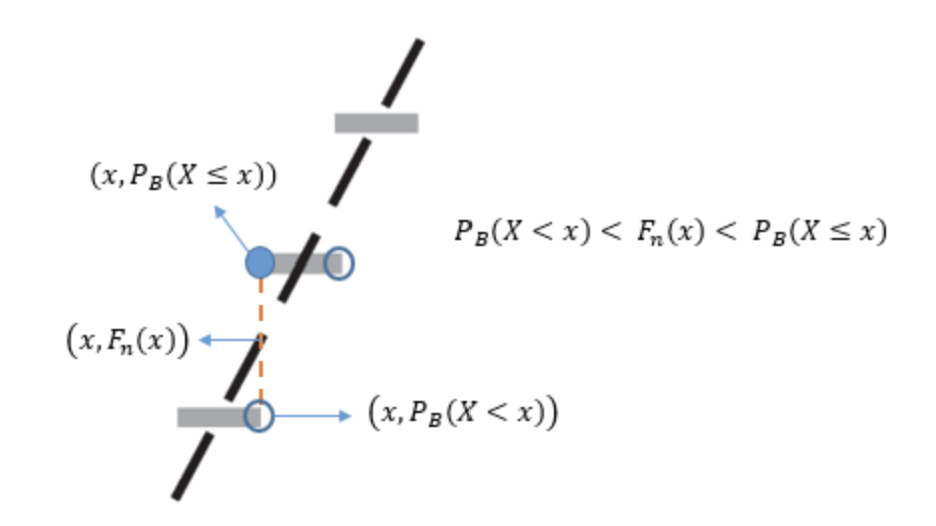
\includegraphics{probability-theory/chapter4/CDF-of-c-and-d-variables.png} 
	\caption{连续型、离散型随机变量CDF图} 
\end{figure}

\hspace{2em}对于离散型随机变量,常出现$P(X<x)\ne P(X\leqslant x)$,而对于连续型随机变量(Continuous Variable),二者的值是相等的,因此,CDF值的近似将出现以下问题:
\begin{enumerate}
	\item 使用正态分布CDF值近似$P(X\leqslant x)$时近似值偏小。
	\item 使用正态分布CDF值近似$P(X< x)$时近似值偏大。
\end{enumerate}
\hspace{2em}而我们会想要得到一个一致的近似,即对于以上两个近似,结果总是一致地偏大或偏小,这样利于分析。

\subsection{具体方法}
\begin{itemize}
	\item 根据近似的分布选择一个$\alpha\in (-1,1)$,一般选择$\pm\frac{1}{2}$。
	\item 使用正态分布CDF值$F(\frac{x+\alpha-\mu}{\sigma})$近似$P(X< x)$与$P(X\leqslant x)$。
\end{itemize}
%\part{最优化}
%\chapter{凸}

\begin{definition}
	设$E$是欧氏空间$X$中的一个点集,若任意两点$x_1,x_2\in E$的连线上的所有点$\alpha x_1+(1-\alpha)x_2\in E,\;0\leqslant\alpha\leqslant1$,则称$E$为\gls{ConvexSet}。
\end{definition}
\begin{definition}
	设$X$是一个欧氏空间,$x_1,x_2\in X$。若存在$\alpha_1,\alpha_2$满足$\alpha_1+\alpha_2=1,\;0\leqslant\alpha_i\leqslant1,\;i=1,2$,使得$x=\alpha_1x_1+\alpha_2x_2$,则称$x$为$x_1,x_2$的\gls{ConvexCombination}。若$0<\alpha_i<1,\;i=1,2$,称其为\gls{StrictlyConvexCombination}。
\end{definition}
\begin{definition}
	设$E$是欧式空间$X$中的一个凸集,$x\in E$。若$x$不能表示为$E$中不同的两点的严格凸组合,则称$x$是$E$的一个\gls{ExtremePoint}。
\end{definition}

\begin{definition}
	对于广义
\end{definition}

\subsection{映射的上下极限与半连续性}
\begin{definition}
	$(X,\rho)$是一个度量空间,$E$是$X$的子空间,$f$是$E$到$\mathbb{R}$上的映射。对于$E$中的任一聚点$a$,定义:
	\begin{gather*}
		\liminf_{x\to a}f(x)=\lim_{\varepsilon\to0}\Bigl(\inf\{f(x):x\in U(a,\varepsilon)\}\backslash\{a\}\Bigr) \\
		\limsup_{x\to a}f(x)=\lim_{\varepsilon\to0}\Bigl(\sup\{f(x):x\in U(a,\varepsilon)\}\backslash\{a\}\Bigr)
	\end{gather*}
\end{definition}
\begin{definition}
	$(X,\rho)$是一个度量空间,$f$是$X$到$\overline{\mathbb{R}}$上的映射。若:
	\begin{equation*}
		\limsup_{x\to a}f(x)\leqslant f(x_0)
	\end{equation*}
	则称$f(x)$在$a$点\gls{UpperSemicontinuous}。
	若:
	\begin{equation*}
		\liminf_{x\to a}f(x)\leqslant f(x_0)
	\end{equation*}
	则称$f(x)$在$a$点\gls{lowerSemicontinuous}。
\end{definition}

%\chapter{规划问题}

\section{线性规划}

\subsection{线性规划的标准形}
线性规划问题的数学模型有各种不同的形式,如:
\begin{enumerate}
	\item 最大化或最小化目标函数;
	\item 约束条件有$\leqslant,\;\geqslant\;=$三种情况;
	\item 决策变量一般有非负性要求,但有时又可能没有。
\end{enumerate}
为了以统一的方式求解线性规划问题,规定了一种线性规划的标准形式,非标准形可以转化为标准形。
\begin{definition}
	规定线性规划问题的\textbf{标准形式}为:
	\begin{enumerate}
		\item 最大化目标函数;
		\item 约束条件为等式且右端常数项非负;
		\item 决策变量非负。
	\end{enumerate}
	于是线性规划问题可以写为如下矩阵形式:
	\begin{gather*}
		\max z=C^TX \\
		s.t.
		\begin{cases}
			AX=\beta \\
			X\geqslant\mathbf{0}
		\end{cases}
	\end{gather*}
	称$C=(c_1,c_2,\dots,c_n)$为\textbf{价值向量},其中每个分量为\textbf{价值系数},$\beta$为\textbf{资源向量}。系数矩阵$A\in M_{m\times n}(\mathbb{R})$行满秩,即$\operatorname{rank}(A)=m$。称$A$的秩$m$为LP问题的\textbf{阶数},$A$的列数$n$为LP问题的\textbf{维数}。
\end{definition}
\begin{theorem}
	每个线性规划问题都可以化成标准形式。
\end{theorem}
\begin{proof}
	考虑每种不符合标准形式的情况:\par
	\textbf{最小化目标函数:}若LP问题的目标函数为:
	\begin{equation*}
		\min z=C^TX
	\end{equation*}
	则可将其转化为:
	\begin{equation*}
		\max z'=-C^TX
	\end{equation*}
	显然转化前后的LP问题是等价的。\par
	\textbf{约束条件右端常数项为负数:}若LP问题的约束条件为$Ax=\beta$和$\alpha^Tx=b<0$,则可将其转化为:
	\begin{equation*}
		\begin{pmatrix}
			A \\
			-\alpha^T
		\end{pmatrix}
		x
		=
		\begin{pmatrix}
			\beta \\
			-b
		\end{pmatrix}
	\end{equation*}
	显然转化前后的LP问题是等价的。\par
	\textbf{约束条件中含$\leqslant$:}若LP问题的约束条件为$Ax=\beta$和$\alpha^Tx\leqslant b$,则可将约束条件转化为:
	\begin{gather*}
		\begin{pmatrix}
			A & \mathbf{0} \\
			\alpha^T & 1
		\end{pmatrix}
		\begin{pmatrix}
			x \\
			y
		\end{pmatrix}
		=
		\begin{pmatrix}
			\beta \\
			b
		\end{pmatrix} \\
		X'=(X,y)^T\geqslant\mathbf{0}
	\end{gather*}
	显然转化前后的LP问题是等价的。称新引入的变量$y$为\gls{SlackVariable}。\par
	\textbf{约束条件中含$\geqslant$:}若LP问题的约束条件为$Ax=\beta$和$\alpha^Tx\geqslant b$,则可将约束条件转化为:
	\begin{gather*}
		\begin{pmatrix}
			A & \mathbf{0} \\
			\alpha^T & -1
		\end{pmatrix}
		\begin{pmatrix}
			x \\
			y
		\end{pmatrix}
		=
		\begin{pmatrix}
			\beta \\
			b
		\end{pmatrix} \\
		X'=(X,y)^T\geqslant\mathbf{0}
	\end{gather*}
	显然转化前后的LP问题是等价的。称新引入的变量$y$为\gls{SurplusVariable}。\par
	\textbf{决策变量中含负值变量:}若LP问题为:
	\begin{gather*}
		\max z=(C,c)^T(X,x)^T \\
		s.t.
		\begin{cases}
			(A,\alpha)(X,x)^T=\beta \\
			X\geqslant\mathbf{0} \\
			x<0
		\end{cases}
	\end{gather*}
	则作变换$x'=-x$,将该LP问题转化为:
	\begin{gather*}
		\max z=(C,-c)^T(X,x')^T \\
		s.t.
		\begin{cases}
			(A,-\alpha)(X,x')^T=\beta \\
			X'=(X,x')^T\geqslant\mathbf{0}
		\end{cases}
	\end{gather*}
	显然转化前后的LP问题是等价的。\par
	\textbf{决策变量中含自由变量\footnote{即对该变量的取值无任何要求。}:}若LP问题为:
	\begin{gather*}
		\max z=(C,c)^T(X,x)^T \\
		s.t.
		\begin{cases}
			(A,\alpha)(X,x)^T=\beta \\
			X\geqslant\mathbf{0}
		\end{cases}
	\end{gather*}
	可引入新变量$x_1,x_2$,将该LP问题转化为:
	\begin{gather*}
		\max z=(C,c,-c)^T(X,x_1,x_2)^T \\
		s.t.
		\begin{cases}
			(A,\alpha,-\alpha)(X,x_1,x_2)^T=\beta \\
			X'=(X,x_1,x_2)^T\geqslant\mathbf{0}
		\end{cases}
	\end{gather*}
	显然转化前后的LP问题是等价的。
\end{proof}
\subsubsection{标准形的基本解}
\begin{definition}
	对于标准形LP问题中约束条件的系数矩阵$A=(\seq{\alpha}{n})\in M_{m\times n}(\mathbb{R})$,称由其列向量组的一个基$\alpha_{i_1},\alpha_{i_2},\dots,\alpha_{i_m}$构成的矩阵$(\alpha_{i_1},\alpha_{i_2},\dots,\alpha_{i_m})$为该LP问题的一个\textbf{基矩阵}(简称\textbf{基}),其中的每一个向量$\alpha_{i_j},\;j=1,2,\dots,m$称为该LP问题的\textbf{基向量},$A$中剩余的$n-m$个列向量$\alpha_{j_1},\alpha_{j_2},\dots,\alpha_{j_{n-m}}$称为\textbf{非基向量}。分别称基向量对应的变量和非基向量对应的变量为\textbf{基变量}、\textbf{非基变量}。分别称所有基变量构成的向量$(x_{i_1},x_{i_2},\dots,x_{i_m})$和非基变量构成的向量$(x_{j_1},x_{j_2},\dots,x_{j_{n-m}})$为\textbf{基变矢}、\textbf{非基变矢}。对系数矩阵$A$的列向量、决策变量$x$和资源向量$\beta=(b_1,b_2,\dots,b_n)^T$作顺序的重排,可以得到:
	\begin{align*}
		&\quad(\alpha_{i_1},\alpha_{i_2},\dots,\alpha_{i_m},\alpha_{j_1},\alpha_{j_2},\dots,\alpha_{j_{n-m}})(x_{i_1},x_{i_2},\dots,x_{i_m},x_{j_1},x_{j_2},\dots,x_{j_{n-m}})^T \\
		&=(b_{i_1},b_{i_2},\dots,b_{i_m},b_{j_1},b_{j_2},\dots,b_{j_{n-m}})^T
	\end{align*}
	将该方程重新写作:
	\begin{equation*}
		(B,C)(X_1,X_2)^T=\beta'
	\end{equation*}
	其中$B$对应基矩阵,$C$对应非基向量构成的矩阵,$X_1$为基变矢,$X_2$为非基变矢。令$X_2=\mathbf{0}$,可得出方程的一个解:
	\begin{equation*}
		\begin{cases}
			X_1=B^{-1}\beta' \\
			X_2=\mathbf{0}
		\end{cases}
	\end{equation*}
	称该解为约束方程组的一个关于基矩阵$B$的\textbf{基本解},也称之为该标准形LP问题的一个基本解。若基本解中存在基变量值为$0$,则称之为\textbf{退化基本解}。若某个基本解达到标准形LP问题的最优解,则称之为\textbf{最优基本解}。称满足非负性约束$X\geqslant\mathbf{0}$的基本解为\gls{BasicFeasibleSolution},若它是退化的,则称之为\textbf{退化基本可行解}。称基本可行解对应的基矩阵为\textbf{可行基},称最优基本解对应的基矩阵为\textbf{最优基}。
\end{definition}

\subsection{线性规划解的性质}
\begin{lemma}
	对于$m$阶$n$维标准形LP问题,$A=(\seq{a}{n})$、$E$分别为其系数矩阵和可行域,则$x=(x_1,x_2,\dots,x_n)\in E$是基本可行解的充分必要条件为:对于$I=\{i:x_i>0,i=1,2,\dots,n\}$,由$a_i,\;i\in I$构成的向量组线性无关。
\end{lemma}
\begin{proof}
	\textbf{必要性:}由基本可行解的定义直接得到。\par
	\textbf{充分性:}
\end{proof}

\begin{property}
	线性规划的解具有如下性质:
	\begin{enumerate}
		\item LP问题解的可行域是凸集;
		\item LP问题的基本可行解与可行域的极点一一对应;
		\item \textbf{线性规划基本定理}
		\begin{itemize}
			\item 若LP问题有可行解,则必有基本可行解;
			\item 若LP问题有最优解,则必有最优基本解。
		\end{itemize}
		\item 若LP问题的可行域不是空集,则可行域至少有一个极点;
		\item LP问题可行域的极点必为有限多个。
	\end{enumerate}
\end{property}
\begin{proof}
	设$m$阶$n$维LP问题如下:
	\begin{gather*}
		\max z=C^TX \\
		s.t.
		\begin{cases}
			AX=\beta \\
			X\geqslant\mathbf{0}
		\end{cases}
	\end{gather*}
	其可行域为$E$,$A=(\seq{a}{n})\in M_{m\times n}(\mathbb{R}),\;x=(x_1,x_2,\dots,x_n)^T$。\par
	(1)显然:
	\begin{equation*}
		E=\{x\in\mathbb{R}^{n}:Ax=\beta,x\geqslant\mathbf{0}\}
	\end{equation*}
	任取$x_1,x_2\in E$,则对任意的$0\leqslant\alpha\leqslant1$有:
	\begin{gather*}
		A[\alpha x_1+(1-\alpha)x_2]=\alpha Ax_1+(1-\alpha)Ax_2=\alpha\beta+(1-\alpha)\beta=\beta \\
		\alpha x_1+(1-\alpha)x_2\geqslant0
	\end{gather*}
	所以$\alpha x_1+(1-\alpha)x_2\in E$,$E$是一个凸集。\par
	(2)\textbf{基本可行解必是极点:}要证基本可行解$x$必是极点,即证$x$不能表示为$E$内不同的两点$x_1,x_2$的严格凸组合。假设$x$可以表示为$x_1,x_2$的严格凸组合,即存在$0<\alpha<1$,使得$x=\alpha x_1+(1-\alpha)x_2$。因为$x$是基本解,所以$x$的非基变量都为$0$,于是$x_1,x_2$对应部分也都为$0$。设$x$对应的基矩阵是$B$,则$x=B^{-1}\beta$,此时也必有$x_1=x_2=B^{-1}\beta$(考虑基本解的求解过程,$B$对应的非基变量全为$0$),于是$x=x_1=x_2$,所以$x$不可以表示为可行域内不同的两点的严格凸组合,矛盾,$x$是极点。\par
	\textbf{极点必是基本可行解:}要证极点$x$必是基本可行解,即证存在基矩阵$B$使得$x=B^{-1}\beta$。由极点定义,$x$不能表示为$E$内不同的两点$x_1,x_2$的严格凸组合,即不存在$0<\alpha<1$和$E$内不同的两点$x_1,x_2$使得$x=\alpha x_1+(1-\alpha)x_2$,
\end{proof}

%\part{不等式}
%\chapter{不等式}
这章讨论各种常见不等式。

\section{Cauchy不等式}

\subsection{实数域上的Cauchy不等式}
\begin{theorem}
	若$a_i,b_i\in\mathbb{R},i=1,2,\dots,n$,则有如下不等式:
	\begin{inequality*}\label{ineq:cauchy-ineq-R}
		\left(\sum_{i=1}^na_ib_i\right)^2\leqslant\sum_{i=1}^na_i^2\cdot\sum_{i=1}^nb_i^2
	\end{inequality*}
\end{theorem}
\begin{proof}
	取$\lambda\in\mathbb{R}$:
	\begin{equation*}
		0\leqslant\sum_{i=1}^n\left(a_i+\lambda b_i\right)^2=
		\sum_{i=1}^na_i^2+2\lambda\sum_{i=1}^na_ib_i+\lambda^2\sum_{i=1}^nb_i^2
	\end{equation*}
	将$\lambda$看作自变量,$a_i,b_i$为常数。由判别式可得:
	\begin{equation*}
		4\left(\sum_{i=1}^na_ib_i\right)^2\leqslant4\sum_{i=1}^na_i^2\cdot\sum_{i=1}^nb_i^2\qedhere
	\end{equation*}
\end{proof}

\subsection{复数域上的Cauchy不等式}
\begin{theorem}
	若$a_i,b_i\in\mathbb{C},i=1,2,\dots,n$,则有如下不等式:
	\begin{inequality*}\label{ineq:cauchy-ineq-C}
		\left(\sum_{i=1}^n|a_ib_i|\right)^2\leqslant\sum_{i=1}^n|a_i|^2\cdot\sum_{i=1}^n|b_i|^2
	\end{inequality*}
\end{theorem}
\begin{proof}
	由复数模的性质可得到
	\begin{equation*}
		|a_ib_i|=|a_i||b_i|
	\end{equation*}
	然后使用实数域上的Cauchy不等式即可立即得到结果。
\end{proof}

\subsection{内积导出的Cauchy-Schiwarz不等式}
\begin{theorem}
	设$X$是一个实或复内积空间,$x,y\in X$,则有如下不等式:
	\begin{inequality*}\label{ineq:cauchy-schiwarz-inner-product}
		|(x,y)|^2\leqslant(x,x)(y,y)
	\end{inequality*}
\end{theorem}
下给出复数域内的证明,实数域的证明显然类似。
\begin{proof}
	设$x,y\in X$。对任意的$\lambda\in\mathbb{C}$,有:
	\begin{equation*}
		(x+\lambda y,x+\lambda y)\geqslant 0
	\end{equation*}
	即:
	\begin{equation*}
		(x,x)+\overline{\lambda}(x,y)+\lambda(y,x)+|\lambda|^2(y,y)\geqslant 0
	\end{equation*}
	令$\lambda=-\frac{(x,y)}{(y,y)}$,得到:
	\begin{gather*}
		(x,x)-2\frac{|(x,y)|^2}{(y,y)}+\frac{|(x,y)|^2}{(y,y)^2}(y,y)\geqslant0 \\
		|(x,y)|^2\leqslant(x,x)(y,y)\qedhere
	\end{gather*}
\end{proof}

\subsection{期望形式的Cauchy-Schiwarz不等式}
\begin{theorem}
	设$\operatorname{E}(X^2)<+\infty,\;\operatorname{E}(Y^2)<+\infty$,则有:
	\begin{inequality*}\label{ineq:cauchy-schiwarz-expectations}
		|\operatorname{E}(XY)|\leqslant\sqrt{\operatorname{E}(X^2)\operatorname{E}(Y^2)}
	\end{inequality*}
	等号成立的充要条件为存在不全为$0$的常数$a,b$使得$aX+bY=0\;$a.s.成立。
\end{theorem}
\begin{proof}
	对任意的常数$a,b$,由\cref{prop:NonnegativeMeasurablegIntegral}(2)(6)可知二次型:
	\begin{equation*}
		\operatorname{E}[(aX+bY)^2]=a^2\operatorname{E}(X^2)+2ab\operatorname{E}(XY)+b^2\operatorname{E}(Y^2)=(a,b)\Sigma(a,b)^T\geqslant0
	\end{equation*}
	其中:
	\begin{equation*}
		\Sigma=
		\begin{pmatrix}
			\operatorname{E}(X^2) & \operatorname{E}(XY) \\
			\operatorname{E}(XY) & \operatorname{E}(Y^2)
		\end{pmatrix}
	\end{equation*}
	所以$\Sigma$是一个半正定矩阵,由\cref{theo:PositiveSemidefinite}第三条的(6)可知$|\Sigma|\geqslant0$,即$|\operatorname{E}(XY)|\leqslant\sqrt{\operatorname{E}(X^2)\operatorname{E}(Y^2)}$。等号成立当且仅当$\Sigma$退化,当且仅当有不全为$0$的常数$a,b$使得$\operatorname{E}[(aX+bY)^2]=0$($\Sigma$退化时列向量线性相关,存在不全为$0$的$a,b$使得$\Sigma(a,b)^T=\mathbf{0}$,即$(a,b)\Sigma(a,b)^T=0$;当存在不全为$0$的$a,b$使得$\operatorname{E}[(aX+bY)^2]=0$时,$(a,b)\Sigma(a,b)^T=0$,\info{需要证明此时一定退化}),由\cref{prop:NonnegativeMeasurablegIntegral}(10)可知此时当且仅当有不全为$0$的常数$a,b$使得$aX+bY=0\;$a.s.。
\end{proof}
\section{Young's不等式}

\subsection{一般形式}
\begin{theorem}
	设$a,b\in\mathbb{R}$且$a,b>0$,$p,q\in\mathbb{R}$且$p,q>1$,满足$\frac{1}{p}+\frac{1}{q}=1$,则有如下不等式:
	\begin{inequality*}\label{ineq:young-ineq-Simple}
		ab\leqslant\frac{a^p}{p}+\frac{b^q}{q}
	\end{inequality*}
	等号成立当且仅当$a^p=b^q$。
\end{theorem}
\begin{proof}
	$f(x)=e^x$是一个凸函数,因此对任意的$t\in(0,1)$:
	\begin{equation*}
		e^{tx+(1-t)y}\leqslant te^x+(1-t)e^y
	\end{equation*}
	等号成立当且仅当$x=y$。令$\frac{1}{p}=t$,利用上式则有:
	\begin{equation*}
		ab=e^{\ln(a)+\ln(b)}=e^{\frac{\ln(a^p)}{p}+\frac{\ln(b^q)}{q}}\leqslant\frac{1}{p}e^{\ln(a^p)}+\frac{1}{q}e^{\ln(b^q)}=\frac{a^p}{p}+\frac{b^q}{q}\qedhere
	\end{equation*}
	因为对数函数单调增,所以等号成立当且仅当$a^p=b^q$。
\end{proof}
\section{Holder不等式}

\subsection{离散形式的Holder不等式}
\subsubsection{有穷级数形式}
\begin{theorem}
	设$\xi_i,\eta_i,i=1,2,\dots,n$同为实数或复数,$1<p,q<+\infty$,满足$\frac{1}{p}+\frac{1}{q}=1$,则有如下不等式:
	\begin{inequality*}\label{ineq:holder-ineq-finite-series}
		\sum_{i=1}^n|\xi_i\eta_i|\leqslant\left(\sum_{i=1}^n|\xi_i|^p\right)^\frac{1}{p}\cdot\left(\sum_{i=1}^n|\eta_i|^q\right)^\frac{1}{q}
	\end{inequality*}
\end{theorem}
\begin{proof}
	在Young's不等式(即\cref{ineq:young-ineq-Simple})中取:
	\begin{equation*}
		a=\frac{|\xi_i|}{\left(\sum\limits_{i=1}^n|\xi_i|^p\right)^\frac{1}{p}},\quad
		b=\frac{|\eta_i|}{\left(\sum\limits_{i=1}^n|\eta_i|^q\right)^\frac{1}{q}}
	\end{equation*}
	即有:
	\begin{gather*}
		\frac{|\xi_i||\eta_i|}{\left(\sum\limits_{i=1}^n|\xi_i|^p\right)^\frac{1}{p}\cdot\left(\sum\limits_{i=1}^n|\eta_i|^q\right)^\frac{1}{q}}
		\leqslant\frac{|\xi_i|^p}{p\left(\sum\limits_{i=1}^n|\xi_i|^p\right)}+\frac{|\eta_i|^q}{q\left(\sum\limits_{i=1}^n|\eta_i|^q\right)} \\
		\frac{\sum\limits_{i=1}^n|\xi_i\eta_i|}{\left(\sum\limits_{i=1}^n|\xi_i|^p\right)^\frac{1}{p}\cdot\left(\sum\limits_{i=1}^n|\eta_i|^q\right)^\frac{1}{q}}
		\leqslant\frac{\sum\limits_{i=1}^n|\xi_i|^p}{p\left(\sum\limits_{i=1}^n|\xi_i|^p\right)}+\frac{\sum\limits_{i=1}^n|\eta_i|^q}{q\left(\sum\limits_{i=1}^n|\eta_i|^q\right)}\leqslant\frac{1}{p}+\frac{1}{q}=1\qedhere
	\end{gather*}
\end{proof}
\subsubsection{无穷级数形式}
\begin{theorem}
	设$\xi_i,\eta_i,i\in\mathbb{N}^+$同为实数或复数,$1<p,q<+\infty$,满足$\frac{1}{p}+\frac{1}{q}=1$,则有如下不等式:
	\begin{inequality*}\label{ineq:holder-ineq-infty-series}
		\sum_{i=1}^{+\infty}|\xi_i\eta_i|\leqslant\left(\sum_{i=1}^{+\infty}|\xi_i|^p\right)^\frac{1}{p}\cdot\left(\sum_{i=1}^{+\infty}|\eta_i|^q\right)^\frac{1}{q}
	\end{inequality*}
\end{theorem}
\begin{proof}
	证明过程与有穷级数几乎一样,只是把求和中的$n$改为$+\infty$的区别。
\end{proof}

\subsection{积分形式的Holder不等式}
\begin{theorem}
	设	$(X,\mathscr{F},\mu)$是一个测度空间,$E\in\mathscr{F}$,$1<p,q<+\infty$,满足$\frac{1}{p}+\frac{1}{q}=1$,$f\in L_p(E),\;g\in L_q(E)$,则有如下不等式:
	\begin{inequality*}\label{ineq:holder-ineq-Lebesgue}
		\int_{E}^{}|f(x)g(x)|\dif \mu\leqslant\left[\int_{E}^{}|f(x)|^p\dif\mu\right]^{\frac{1}{p}}\left[\int_{E}^{}|g(x)|^q\dif\mu\right]^{\frac{1}{q}}
	\end{inequality*}
	等号成立当且仅当存在不全为$0$的$\alpha,\beta\geqslant0$使得:
	\begin{equation*}
		\alpha|f|^p=\beta|g|^q\;\text{a.e.于$E$}
	\end{equation*}
\end{theorem}
\begin{proof}
	\textbf{(1)$\;f(x)=0$和$g(x)=0\;$都不a.e.于$E$:}在Young's不等式(即\cref{ineq:young-ineq-Simple})中取:
	\begin{equation*}
		a=\frac{|f(x)|}{\left[\int_{E}^{}|f(x)|^p\dif\mu\right]^\frac{1}{p}},\quad
		b=\frac{|g(x)|}{\left[\int_{E}^{}|g(x)|^q\dif\mu\right]^\frac{1}{q}}
	\end{equation*}
	即有:
	\begin{equation*}
		\frac{|f(x)||g(x)|}{\left[\int_{E}^{}|f(x)|^p\dif\mu\right]^\frac{1}{p}\cdot\left[\int_{E}^{}|g(x)|^q\dif\mu\right]^\frac{1}{q}}
		\leqslant\frac{|f(x)|^p}{p\left[\int_{E}^{}|f(x)|^p\dif\mu\right]}+\frac{|g(x)|^q}{q\left[\int_{E}^{}|g(x)|^q\dif\mu\right]}
	\end{equation*}
	两边进行积分可得:
	\begin{gather*}
		\int_{E}\frac{|f(x)g(x)|}{\left[\int_{E}^{}|f(x)|^p\dif\mu\right]^\frac{1}{p}\cdot\left[\int_{E}^{}|g(x)|^q\dif\mu\right]^\frac{1}{q}}\dif\mu\leqslant\frac{1}{p}+\frac{1}{q} \\
		\int_{E}|f(x)g(x)|\dif\mu\leqslant\left(\frac{1}{p}+\frac{1}{q}\right)\left[\int_{E}^{}|f(x)|^p\dif\mu\right]^\frac{1}{p}\cdot\left[\int_{E}^{}|g(x)|^q\dif\mu\right]^\frac{1}{q} \\
		\int_{E}|f(x)g(x)|\dif\mu\leqslant\left[\int_{E}^{}|f(x)|^p\dif\mu\right]^\frac{1}{p}\cdot\left[\int_{E}^{}|g(x)|^q\dif\mu\right]^\frac{1}{q}
	\end{gather*}
	由Young's不等式可知等号成立当且仅当:
	\begin{gather*}
		\frac{|f(x)|^p}{\int_{E}^{}|f(x)|^p\dif\mu}=\frac{|g(x)|^q}{\int_{E}^{}|g(x)|^q\dif\mu} \\
		|f(x)|^p\int_{E}^{}|g(x)|^q\dif\mu=|g(x)|^q\int_{E}^{}|f(x)|^p\dif\mu
	\end{gather*}
	但使用Young's不等式接下来的是积分的操作,我们只需要积分保持不等号即可,所以由\cref{prop:NonnegativeMeasurableIntegral}(7)可知Young's不等式得到的那个不等式只要a.e.成立即可,即上式只要a.e.成立即可。\par
	\textbf{(2)$\;f(x)=0$或$g(x)=0\;$a.e.于$E$:}$|f(x)g(x)|=0\;$a.e.于$E$,由\cref{prop:NonnegativeMeasurableIntegral}(10)可得$\int_{E}|f(x)g(x)|\dif\mu=0$,再根据\cref{prop:NonnegativeMeasurableIntegral}(2)可得$\int_{A}|f(x)|^p\dif\mu,\int_{E}|g(x)|^q\dif\mu\geqslant0$,于是不等式成立。\par
	以上两种情况都可以推导出存在不全为$0$的$\alpha,\beta\geqslant0$使得:
	\begin{equation*}
		\alpha|f|^p=\beta|g|^q\;\text{a.e.于$E$}
	\end{equation*}
	即等号成立时上式也成立,下面证明反过来也对。当上不等式成立时,进行分类讨论。\par
	\textbf{(1)$\;f(x)=0$或$g(x)=0\;$a.e.于$E$:}仅对$|f(x)|=0\;$a.e.于$E$的情况进行证明,$g(x)=0\;$a.e.于$E$的情况可对称得到。此时$|f(x)|^p=0$和$|f(x)g(x)|$都a.e.于$E$,于是由\cref{prop:NonnegativeMeasurableIntegral}(10)可得:
	\begin{equation*}
		\int_{E}|f(x)g(x)|\dif\mu=0,\;\int_{E}|f(x)|^p\dif\mu=0
	\end{equation*}
	所以:
	\begin{equation*}
		\int_{E}^{}|f(x)g(x)|\dif \mu=\left[\int_{E}^{}|f(x)|^p\dif\mu\right]^{\frac{1}{p}}\left[\int_{E}^{}|g(x)|^q\dif\mu\right]^{\frac{1}{q}}=0
	\end{equation*}\par
	\textbf{(2)$\;f(x)=0$和$g(x)=0\;$都不a.e.于$E$:}设$\alpha\ne0$,对$\beta\ne0$的情况可对称得到。此时有:
	\begin{equation*}
		|f|^p=\frac{\beta}{\alpha}|g|^q\;\text{a.e.于$E$}
	\end{equation*}
	所以:
	\begin{equation*}
		|f(x)g(x)|=|f(x)||g(x)|=\left(\frac{\beta}{\alpha}\right)^{-p}|g(x)|^{\frac{q}{p}+1}
	\end{equation*}
	因为$\dfrac{1}{p}+\dfrac{1}{q}=1$,所以$\dfrac{q}{p}+1=q$,于是由\cref{prop:NonnegativeMeasurableIntegral}(6)可得:
	\begin{equation*}
		\int_{E}|f(x)g(x)|\dif\mu=\int_{E}\left(\frac{\beta}{\alpha}\right)^{-p}|g(x)|^{q}\dif\mu=\left(\frac{\beta}{\alpha}\right)^{-p}\int_{E}|g(x)|^q\dif\mu
	\end{equation*}
	对$\alpha|f|^p=\beta|g|^q$两边积分,由\cref{prop:NonnegativeMeasurableIntegral}(8)(6)可得:
	\begin{gather*}
		\int_{E}\alpha|f(x)|^p\dif\mu=\int_{E}\beta |g(x)|^q\dif\mu \\
		\alpha\int_{E}|f(x)|^p\dif\mu=\beta\int_{E}|g(x)|^q\dif\mu \\
		\frac{\int_{E}|f(x)|^p\dif\mu}{\int_{E}|g(x)|^q\dif\mu}=\frac{\beta}{\alpha} \\
		\left[\frac{\int_{E}|f(x)|^p\dif\mu}{\int_{E}|g(x)|^q\dif\mu}\right]^{-p}=\left(\frac{\beta}{\alpha}\right)^{-p}
	\end{gather*}
	将其代入到之前的式子可得:
	\begin{align*}
		\int_{E}|f(x)g(x)|\dif\mu&=\left(\frac{\beta}{\alpha}\right)^{-p}\int_{E}|g(x)|^q\dif\mu \\
		&=\left[\frac{\int_{E}|f(x)|^p\dif\mu}{\int_{E}|g(x)|^q\dif\mu}\right]^{-p}\int_{E}|g(x)|^q\dif\mu \\
		&=\left[\int_{E}|f(x)|^p\dif\mu\right]^{\frac{1}{p}}\left[\int_{E}|g(x)|^q\dif\mu\right]^{\frac{1}{q}}\qedhere
	\end{align*}
\end{proof}
\begin{theorem}
	设	$(X,\mathscr{F},\mu)$是一个测度空间,$E\in\mathscr{F}$,$1<p,q<+\infty$,满足$\frac{1}{p}+\frac{1}{q}=1$。对任意的$f\in L_p(E),\;g\in L_q(E),\;h\in L_1(E)$,在$L_1(E),L_p(E)$和$L_q(E)$中引入范数:
	\begin{equation*}
		||f||_p=\left[\int_{E}^{}|f(x)|^p\dif\mu\right]^\frac{1}{p},\;||g||_q=\left[\int_{E}|g(x)|^q\dif\mu\right]^{\frac{1}{q}},\;||h||_1=\int_{E}|h(x)|\dif\mu
	\end{equation*}
	则积分形式的Holder不等式可写为:
	\begin{inequality*}\label{ineq:holder-ineq-norm}
		||fg||_1\leqslant||f||_p\;||g||_q
	\end{inequality*}
	其中$fg\in L_1(E)$由$f\in L_p(E),g\in L_q(E)$以及积分形式的Holder不等式保证。
\end{theorem}
\begin{note}
	范数是对于空间内的元素定义的,所以写范数的时候首先要保证元素在这个空间内,这里做的其实是一个假设并验证的过程,假设在空间内,然后计算,由结果发现确实是在空间内的。
\end{note}
\begin{theorem}
	设	$(X,\mathscr{F},\mu)$是一个测度空间,$E\in\mathscr{F}$。对任意的$f\in L_1(E),\;g\in L_{\infty}(E)$,在$L_{\infty}(E)$和$L_1(E)$中分别定义范数为元素的无穷范数和:
	\begin{equation*}
		||f||_1=\int_{E}|f(x)|\dif\mu
	\end{equation*}
	则有:
	\begin{inequality*}\label{ineq:holder-ineq-norm+infty}
		||fg||_1\leqslant||f||_1\;||g||_{\infty}
	\end{inequality*}
\end{theorem}
\begin{proof}
	由\cref{prop:NonnegativeMeasurableIntegral}(8)(6)和无穷范数的定义可得:
	\begin{equation*}
		||fg||_1=\int_{E}|f(x)g(x)|\dif\mu\leqslant\int_{E}|f(x)|\;||g||_{\infty}\dif\mu=||g||_{\infty}\int_{E}|f(x)|\dif\mu=||f||_1\;||g||_{\infty}\qedhere
	\end{equation*}
	其中$fg\in L_1(E)$由$f\in L_1(E),g\in L_{\infty}(E)$以及上式保证。
\end{proof}







\section{Minkowski不等式}

\subsection{离散形式的Minkowski不等式}
\subsubsection{有穷级数形式}
设$\xi_i,\eta_i,i=1,2,\dots,n$同为实数或复数,$1\geqslant p<+\infty$,则有如下不等式:
\begin{inequality*}\label{ineq:minkowski-ineq-finite-series}
	\left(\sum_{i=1}^n|\xi_i+\eta_i|^p\right)^\frac{1}{p}\leqslant\left(\sum_{i=1}^n|\xi_i|^p\right)^\frac{1}{p}+\left(\sum_{i=1}^n|\eta_i|^p\right)^\frac{1}{p}
\end{inequality*}
\begin{proof}
	当$p=1$时结论显然成立。当$p>1$时,取$p,q\in\mathbb{R}$且$p,q>1$,满足$\frac{1}{p}+\frac{1}{q}=1$,由Holder不等式(即\cref{ineq:holder-ineq-finite-series}):
	\begin{gather*}
		\sum_{i=1}^n|\xi_i||\xi_i+\eta_i|^\frac{p}{q}\leqslant\left(\sum_{i=1}^n|\xi_i|^p\right)^\frac{1}{p}\cdot\left(\sum_{i=1}^n|\xi_i+\eta_i|^p\right)^\frac{1}{q} \\
		\sum_{i=1}^n|\eta_i||\xi_i+\eta_i|^\frac{p}{q}\leqslant\left(\sum_{i=1}^n|\eta_i|^p\right)^\frac{1}{p}\cdot\left(\sum_{i=1}^n|\xi_i+\eta_i|^p\right)^\frac{1}{q} 
	\end{gather*}
	因此:
	\begin{align*}
		\sum_{i=1}^n|\xi_i+\eta_i|^p&=\sum_{i=1}^n\left[|\xi_i+\eta_i|\;|\xi_i+\eta_i|^{p-1}\right] \\
		&\leqslant\sum_{i=1}^n\left[(|\xi_i|+|\eta_i|)|\xi_i+\eta_i|^\frac{p}{q}\right] \\
		&=\sum_{i=1}^n|\xi_i||\xi_i+\eta_i|^\frac{p}{q}+\sum_{i=1}^n|\eta_i||\xi_i+\eta_i|^\frac{p}{q} \\
		&\leqslant\left[\left(\sum_{i=1}^n|\xi_i|^p\right)^\frac{1}{p}+\left(\sum_{i=1}^n|\eta_i|^p\right)^\frac{1}{p}\right]\cdot\left(\sum_{i=1}^n|\xi_i+\eta_i|^p\right)^\frac{1}{q} 
	\end{align*}
	上式第一行到第二行需要注意到$p-1=\frac{p}{q}$。两边同除$\left(\sum\limits_{i=1}^n|\xi_i+\eta_i|^p\right)^\frac{1}{q}$(若其为$0$则结论显然也成立)即有:
	\begin{equation*}
		\left(\sum_{i=1}^n|\xi_i+\eta_i|^p\right)^\frac{1}{p}\leqslant\left(\sum_{i=1}^n|\xi_i|^p\right)^\frac{1}{p}+\left(\sum_{i=1}^n|\eta_i|^p\right)^\frac{1}{p}\qedhere
	\end{equation*}
\end{proof}
\subsubsection{无穷级数形式}
设$\xi_i,\eta_i,i=1,2,\dots,n$同为实数或复数,$1\geqslant p<+\infty$,则有如下不等式:
\begin{inequality*}\label{ineq:minkowski-ineq-infty-series}
	\left(\sum_{i=1}^{+\infty}|\xi_i+\eta_i|^p\right)^\frac{1}{p}\leqslant\left(\sum_{i=1}^{+\infty}|\xi_i|^p\right)^\frac{1}{p}+\left(\sum_{i=1}^{+\infty}|\eta_i|^p\right)^\frac{1}{p}
\end{inequality*}
\begin{proof}
	证明过程与有穷级数几乎一样,只是把求和中的$n$改为$+\infty$的区别。
\end{proof}

\subsection{积分形式的Minkowski不等式}
\begin{theorem}
	设	$(X,\mathscr{F},\mu)$是一个测度空间,$1\leqslant p<+\infty$,$E\in\mathscr{F}$,$f,g\in L_p(E)$,则有如下不等式:
	\begin{inequality*}\label{ineq:minkowski-ineq-Lebesgue}
		\left[\int_{E}^{}|f(x)+g(x)|^p\dif\mu\right]^\frac{1}{p}\leqslant\left[\int_{E}^{}|f(x)|^p\dif\mu\right]^\frac{1}{p}+\left[\int_{E}^{}|g(x)|^p\dif\mu\right]^\frac{1}{p}
	\end{inequality*}
	且:
	\begin{enumerate}
		\item $p=1$时等号成立当且仅当$fg\geqslant0\;$a.e.于$E$;
		\item $p>1$时等号成立当且仅当存在不全为$0$的$\alpha,\beta\geqslant0$使得$\alpha f=\beta g$。
	\end{enumerate}
\end{theorem}
\begin{proof}
	\textbf{(1)$\;p=1$:}由绝对值的三角不等式以及\cref{prop:NonnegativeMeasurableIntegral}(6)直接可得。等号成立当且仅当$f(x)g(x)\geqslant0$,考虑到\cref{prop:NonnegativeMeasurableIntegral}(8),只要$f(x)g(x)\geqslant0\;$a.e.于$E$即可。\par
	\textbf{(2)$\;p>1$:}当$|f(x)+g(x)|=0\;$a.e.于$E$时,由\cref{prop:NonnegativeMeasurableIntegral}(10)可知$\left[\int_{E}^{}|f(x)+g(x)|^p\dif\mu\right]^\frac{1}{p}=0$,根据\cref{prop:NonnegativeMeasurableIntegral}(2)可得结论成立。此时由\cref{prop:NonnegativeMeasurableIntegral}(2)(10)可知等号成立当且仅当$f=0\;$a.e.于$E$且$g=0\;$a.e.于$E$,该条件可推出存在不全为$0$的$\alpha,\beta\geqslant0$使得$\alpha f=\beta g\;$a.e.于$E$。\par
	当$|f(x)+g(x)|=0\;$不a.e.于$E$时,取$q\in\mathbb{R}$且$q>1$,满足$\frac{1}{p}+\frac{1}{q}=1$,由Holder不等式(即\cref{ineq:holder-ineq-Lebesgue}):
	\begin{gather*}
		\int_{E}^{}|f(x)|\;|f(x)+g(x)|^\frac{p}{q}\dif\mu\leqslant\left[\int_{E}^{}|f(x)|^p\dif\mu\right]^\frac{1}{p}\left[\int_{E}^{}|f(x)+g(x)|^p\dif\mu\right]^\frac{1}{q} \\
		\int_{E}^{}|g(x)|\;|f(x)+g(x)|^\frac{p}{q}\dif\mu\leqslant\left[\int_{E}^{}|g(x)|^p\dif\mu\right]^\frac{1}{p}\left[\int_{E}^{}|f(x)+g(x)|^p\dif\mu\right]^\frac{1}{q}
	\end{gather*}
	注意到$p+q=pq$,所以$q(p-1)=qp-q=p$,因此由绝对值的三角不等式以及\cref{prop:NonnegativeMeasurableIntegral}(6)可得:
	\begin{align*}
		\int_{E}^{}|f(x)+g(x)|^p\dif\mu
		&=\int_{E}^{}|f(x)+g(x)|\;|f(x)+g(x)|^{p-1}\dif\mu \\
		&\leqslant\int_{E}^{}\Bigl[|f(x)|+|g(x)|\Bigr]\;|f(x)+g(x)|^{p-1}\dif\mu \\
		&=\int_{E}^{}|f(x)|\;|f(x)+g(x)|^{p-1}\dif\mu+\int_{E}^{}|g(x)|\;|f(x)+g(x)|^{p-1}\dif\mu \\
		&\leqslant\left\{\left[\int_{E}^{}|f(x)|^p\dif\mu\right]^\frac{1}{p}+\left[\int_{E}^{}|g(x)|^p\dif\mu\right]^\frac{1}{p}\right\}\left[\int_{E}^{}|f(x)+g(x)|^p\dif\mu\right]^\frac{1}{q}
	\end{align*}
	两边同除$\left[\int_{E}^{}|f(x)+g(x)|^p\dif\mu\right]^\frac{1}{q}$即有:
	\begin{equation*}
			\left[\int_{E}^{}|f(x)+g(x)|^p\dif\mu\right]^\frac{1}{p}\leqslant\left[\int_{E}^{}|f(x)|^p\dif\mu\right]^\frac{1}{p}+\left[\int_{E}^{}|g(x)|^p\dif\mu\right]^\frac{1}{p}
	\end{equation*}
	由放缩的过程注意到等号成立当且仅当Holder不等式取等且$f(x)g(x)\geqslant0\;$a.e.于$E$,而Holder不等式取等当且仅当存在不全为$0$的$\alpha,\beta\geqslant0$和不全为$0$的$\gamma,\delta\geqslant0$使得:
	\begin{equation*}
		\alpha|f|^p=\beta|f+g|^p,\;\gamma|g|^p=\delta|f+g|^p\;\text{a.e.于$E$}
	\end{equation*}
	因为此时$f(x),g(x)$同号a.e.于$E$,所以也即存在不全为$0$的$\alpha,\beta\geqslant0$和不全为$0$的$\gamma,\delta\geqslant0$使得:
	\begin{equation*}
		\alpha f=\beta (f+g),\;\gamma g=\delta(f+g)\;\text{a.e.于$E$}
	\end{equation*}
	该条件可推出存在不全为$0$的$\alpha,\beta\geqslant0$使得$\alpha f=\beta g\;$a.e.于$E$。\par
	接下来证明存在不全为$0$的$\alpha,\beta\geqslant0$使得$\alpha f=\beta g\;$a.e.于$E$也可推出等式成立。仅对$\alpha\ne0$的情况进行证明,$\beta\ne0$的情况可对称得到。\par
	\textbf{(1)$\;|f(x)+g(x)|=0\;$a.e.于$E$:}此时可得到$g=0\;$a.e.于$E$,进而得到$f=0\;$a.e.成立。由\cref{prop:NonnegativeMeasurableIntegral}(10)可得:
	\begin{equation*}
		\left[\int_{E}^{}|f(x)+g(x)|^p\dif\mu\right]^\frac{1}{p}=\left[\int_{E}^{}|f(x)|^p\dif\mu\right]^\frac{1}{p}+\left[\int_{E}^{}|g(x)|^p\dif\mu\right]^\frac{1}{p}=0
	\end{equation*}\par
	\textbf{(2)$\;|f(x)+g(x)|=0$不a.e.于$E$:}此时可得到:
	\begin{equation*}
		f=\frac{\beta}{\alpha}g\;\text{a.e.于$E$}
	\end{equation*}
	于是由\cref{prop:NonnegativeMeasurableIntegral}(6)(8)可得:
	\begin{align*}
		\left[\int_{E}^{}|f(x)+g(x)|^p\dif\mu\right]^{\frac{1}{p}}&=\left[\int_{E}^{}\left|\frac{\beta+\alpha}{\alpha}g(x)\right|^p\dif\mu\right]^\frac{1}{p} \\
		&=\frac{\beta+\alpha}{\alpha}\left[\int_{E}^{}|g(x)|^p\dif\mu\right]^\frac{1}{p} \\
		&=\frac{\beta}{\alpha}\left[\int_{E}^{}|g(x)|^p\dif\mu\right]^\frac{1}{p}+\left[\int_{E}^{}|g(x)|^p\dif\mu\right]^\frac{1}{p} \\
		&=\left[\int_{E}\left|\frac{\beta}{\alpha}g(x)\right|^p\dif\mu\right]^{\frac{1}{p}}+\left[\int_{E}^{}|g(x)|^p\dif\mu\right]^\frac{1}{p} \\
		&=\left[\int_{E}^{}|f(x)|^p\dif\mu\right]^\frac{1}{p}+\left[\int_{E}^{}|g(x)|^p\dif\mu\right]^\frac{1}{p}\qedhere
	\end{align*}
\end{proof}
\begin{theorem}
	设	$(X,\mathscr{F},\mu)$是一个测度空间,$1\leqslant p<+\infty$,$E\in\mathscr{F}$。对任意的$f,g\in L_p(E)$,在$L_p(E)$空间中引入范数:
	\begin{equation*}
		||f||_p=\left[\int_{E}^{}|f(x)|^p\dif\mu\right]^\frac{1}{p}
	\end{equation*}
	则积分形式的Minkowski不等式可写为:
	\begin{inequality*}\label{ineq:minkowski-ineq-norm}
		||f+g||_p\leqslant||f||_p+||g||_p
	\end{inequality*}
\end{theorem}
\begin{theorem}
	设	$(X,\mathscr{F},\mu)$是一个测度空间,$E\in\mathscr{F}$。在$L_{\infty}(E)$中定义范数为元素的无穷范数,则有:
	\begin{inequality*}\label{ineq:minkowski-ineq-norm+infty}
		||f+g||_{\infty}\leqslant||f||_{\infty}+||g||_{\infty}
	\end{inequality*}
\end{theorem}
\begin{proof}
	由绝对值的三角不等式以及上确界的性质:
	\begin{equation*}
		\sup_{x\in E\backslash e}|f(x)+g(x)|\leqslant\sup_{x\in E\backslash e}[|f(x)|+|g(x)|]\leqslant\sup_{x\in E\backslash e}|f(x)|+\sup_{x\in E\backslash e}|g(x)|
	\end{equation*}
	由下确界的性质即可得:
	\begin{equation*}
		||f+g||_{\infty}\leqslant||f||_{\infty}+||g||_{\infty}\qedhere
	\end{equation*}
\end{proof}
\begin{theorem}
	设$(X,\mathscr{F},\mu)$是一个测度空间,$1\leqslant p\leqslant+\infty$,$E\in\mathscr{F}$。对任意的$f,g\in L_p(E)$,有:
	\begin{inequality*}\label{ineq:minkowski-ineq-norm-all}
		||f+g||_p\leqslant||f||_p+||g||_p,\quad
		\Big|||f||_p-||g||_p\Big|\leqslant||f-g||_p
	\end{inequality*}
\end{theorem}
\begin{proof}
	第一式由\cref{ineq:minkowski-ineq-norm}和\cref{ineq:holder-ineq-norm+infty}直接推出。第二式只需注意到:
	\begin{gather*}
		||f||_p=||f-g+g||_p\leqslant||f-g||_p+||g||_p \\
		||g||_p=||g-f+f||_p\leqslant||g-f||_p+||f||_p=||f-g||_p+||f||_p\qedhere
	\end{gather*}
\end{proof}
\section{Something else}

\begin{theorem}
	对于所有 $a,b\in\mathbb{R}$ 及 $p\ge 1$,有不等式
	\begin{inequality*}\label{ineq:else-1}
		|a+b|^p\leqslant\Bigl(|a|+|b|\Bigr)^p \leqslant 2^{p-1}\Bigl(|a|^p+|b|^p\Bigr).
	\end{inequality*}
\end{theorem}
\begin{proof}
	第一式显然成立。令 $a,b\in\mathbb{R}$,并设 $x=|a|$ 和 $y=|b|$(显然 $x,y\geqslant0$)。考虑函数
	\begin{equation*}
		f(t)=t^p,\quad t\ge 0
	\end{equation*}
	由于 $p\geqslant1$,函数 $f(t)$ 是凸函数。根据凸函数的定义,对于任意 $x,y\ge 0$ 和 $\lambda\in[0,1]$ 有
	\begin{equation*}
		f\bigl(\lambda x+(1-\lambda)y\bigr)\leqslant\lambda f(x)+(1-\lambda)f(y)
	\end{equation*}
	取 $\lambda=\frac{1}{2}$,则上式变为:
	\begin{equation*}
		\left(\frac{x+y}{2}\right)^p\leqslant\frac{x^p+y^p}{2}
	\end{equation*}
	将上式两边同时乘以 $2^p$,得到
	\begin{equation*}
		(x+y)^p\leqslant2^{p-1}\Bigl(x^p+y^p\Bigr)
	\end{equation*}
	将 $x=|a|$ 和 $y=|b|$ 代回,即得所需的不等式。
\end{proof}

\subsection{Jensen不等式}
\begin{theorem}
	设$(X,\mathscr{F},P)$是一个概率空间,$\mathscr{A}\subseteq\mathscr{F}$,$f$是$(X,\mathscr{F})$上可积的Borel函数,$\varphi$为$(\mathbb{R}^{},\mathcal{B})$上的Borel函数且是$\mathbb{R}^{}$上的凸函数,$\varphi\circ f$在$X$上可积,则有:
	\begin{inequality*}\label{ineq:Jensen}
		\varphi[\operatorname{E}(f|\mathscr{A})]\leqslant\operatorname{E}(\varphi\circ f|\mathscr{A})
	\end{inequality*}
	等号成立a.s.于$(X,\mathscr{A},P)$的一个充分条件为$f=\operatorname{E}(f|\mathscr{A})\;$a.s.于$X$。若$\varphi$是严格凸的,则等号成立a.s.于$(X,\mathscr{A},P)$的充要条件为$f=\operatorname{E}(f|\mathscr{A})\;$a.s.于$X$。
\end{theorem}
\begin{proof}
	令:
	\begin{equation*}
		x_0=\operatorname{E}(f|\mathscr{A})
	\end{equation*}
	根据\cref{prop:ConvexFunction}(3)可知存在$a,b\in\mathbb{R}^{}$使得:
	\begin{equation*}
		\forall\;x\in\mathbb{R}^{},\;ax+b\leqslant\varphi(x)
	\end{equation*}
	并满足$ax_0+b=\varphi(x_0)$。根据\cref{prop:MeasurableIntegral}(6),令$x=f(\omega)$对两侧求关于$\mathscr{A}$的条件期望,由\cref{prop:ConditionalExpectation}(5)(1)可得:
	\begin{gather*}
		\operatorname{E}(af+b|\mathscr{A})=a\operatorname{E}(f|\mathscr{A})+b\operatorname{E}(1|\mathscr{A})\;\text{a.s.于}(X,\mathscr{A},P) \\ a\operatorname{E}(f|\mathscr{A})+b\operatorname{E}(1|\mathscr{A})=a\operatorname{E}(f|\mathscr{A})+b\;\text{a.s.于}(X,\mathscr{A},P)
	\end{gather*}
	根据\cref{prop:Measure}(3)(次有限可加性)和测度的非负性可知$\operatorname{E}(af+b|\mathscr{A})=a\operatorname{E}(f|\mathscr{A})+b\;$a.s.于$(X,\mathscr{A},P)$。显然$af(\omega)+b$在$X$上可积,由\cref{prop:ConditionalExpectation}(4)、\cref{prop:Measure}(3)(次有限可加性)和测度的非负性即可得:
	\begin{equation*}
		a\operatorname{E}(f|\mathscr{A})+b=\varphi[\operatorname{E}(f|\mathscr{A})]\leqslant\operatorname{E}(\varphi\circ f|\mathscr{A})\;\text{a.s.于}(X,\mathscr{A},P)
	\end{equation*}
	当$f=\operatorname{E}(f|\mathscr{A})\;$a.s.于$(X,\mathscr{A},P)$时,$\varphi(f)=\varphi[\operatorname{E}(f|\mathscr{A})]\;$a.s.于$(X,\mathscr{A},P)$,因为$\varphi\circ f\in L_1(X)$,根据\cref{prop:MeasurableIntegral}(7)可知$\varphi[\operatorname{E}(f|\mathscr{A})]\in L_1(X)$。由\cref{prop:MeasurableMapping}(2)和\cref{prop:ConditionalExpectation}(1)可得$\operatorname{E}\{\varphi[\operatorname{E}(f|\mathscr{A})]|\mathscr{A}\}=\varphi[\operatorname{E}(f|\mathscr{A})]\;$a.s.于$(X,\mathscr{A},P)$。由\cref{prop:ConditionalExpectation}(4)、\cref{prop:Measure}(3)(次有限可加性)和测度的非负性可得:
	\begin{equation*}
		\operatorname{E}(\varphi\circ f|\mathscr{A})=\operatorname{E}\{\varphi[\operatorname{E}(f|\mathscr{A})]|\mathscr{A}\}=\varphi[\operatorname{E}(f|\mathscr{A})]\;\text{a.s.于}(X,\mathscr{A},P)
	\end{equation*}\par
	当$\varphi$严格凸时,对任意的$x\in\mathbb{R}^{}\backslash\{x_0\}$有$ax+b<\varphi(x)$。若$\varphi[\operatorname{E}(f|\mathscr{A})]=\operatorname{E}(\varphi\circ f|\mathscr{A})\;$a.s.于$(X,\mathscr{A},P)$,则:
	\begin{equation*}
		\operatorname{E}\{\varphi[\operatorname{E}(f|\mathscr{A})]\}=\operatorname{E}[\operatorname{E}(\varphi\circ f|\mathscr{A})]=\operatorname{E}(\varphi\circ f)
	\end{equation*}\info{未完成}
\end{proof}

\subsection{Chebyshev不等式}
\begin{theorem}
	设$X$是一个随机变量,其数学期望和方差都存在,则对任意的$\varepsilon>0$,有:
	\begin{inequality*}\label{ineq:Chebyshev}
		P(|X-\operatorname{E}(X)|\geqslant\varepsilon)\leqslant\frac{\operatorname{Var}(X)}{\varepsilon^2}
	\end{inequality*}
\end{theorem}
\begin{proof}
	设$X$的分布函数为$F(x)$,则:
	\begin{align*}
		P(|X-\operatorname{E}(X)|\geqslant\varepsilon)
		&=\int_{\{x:|x-\operatorname{E}(X)|\geqslant\varepsilon\}}^{}\dif F(x) \\
		&\leqslant\int_{\{x:|x-\operatorname{E}(X)|\geqslant\varepsilon\}}^{}\frac{|x-\operatorname{E}(X)|^2}{\varepsilon^2}\dif F(x) \\
		&\leqslant\frac{1}{\varepsilon^2}\int_{-\infty}^{+\infty}|x-\operatorname{E}(X)|^2\dif F(x) \\
		&=\frac{\operatorname{Var}(X)}{\varepsilon^2}\qedhere
	\end{align*}
\end{proof}

%\part{统计学}
%\chapter{正态分布与三大抽样分布}

\section{多元正态分布}

\subsection{多元正态分布的定义}
\begin{definition}\label{def:MultiNormal1}
	若一个随机向量$\mathbf{X}=(\mathbf{X}_1,\mathbf{X}_2,\dots,\mathbf{X}_n)^T\in\mathbb{R}^n$满足以下概率密度函数:
	\begin{equation}
		p(\mathbf{X}|\boldsymbol{\mu},\Sigma)=\frac{1}{(2\pi)^{\frac{n}{2}}(\det\Sigma)^{\frac{1}{2}}}e^{-\frac{1}{2}(\mathbf{X}-\boldsymbol{\mu})^T\Sigma^{-1}(\mathbf{X}-\boldsymbol{\mu})}\notag
	\end{equation}
	则称其为一个正态随机向量,记作$\mathbf{X}\sim N_n(\boldsymbol{\mu},\;\Sigma)$。其中,$\boldsymbol{\mu}=(\seq{\mu}{n})^T\in\mathbb{R}^{n}$,$\Sigma\in M_{n}(\mathbb{R})$且$\Sigma>0$。
\end{definition}
\begin{theorem}
	对于正态随机向量的概率密度函数,$\boldsymbol{\mu}$和$\Sigma$分别是$\mathbf{X}$的均值向量和协方差矩阵。
\end{theorem}
\begin{proof}
	令:
	\begin{equation}
		\mathbf{Y}=\Sigma^{-\frac{1}{2}}(\mathbf{X}-\boldsymbol{\mu})\notag
	\end{equation}\par
	则有$\mathbf{X}=\Sigma^{\frac{1}{2}}\mathbf{Y}+\boldsymbol{\mu}$,由求随机变量函数的分布中的变量变换法可知\footnote{这是由于$\mathbf{X}$到$\mathbf{Y}$的变换是一个线性变换,线性变换让$\mathbf{X}$关于$\mathbf{Y}$有连续偏导数,同时这个线性变换可逆,满足变量变换法的两大条件。}\info{写完变量变换法链接过来}:
	\begin{equation}
		p(\mathbf{Y})=p(\Sigma^{\frac{1}{2}}\mathbf{Y}+\boldsymbol{\mu})|\mathbf{J}|\notag
	\end{equation}\par
	其中$\mathbf{J}$为变换的Jacobi行列式:
	\begin{equation}
		\mathbf{J}=
		\begin{vmatrix}
			\dfrac{\partial \mathbf{X}_1}{\partial \mathbf{Y}_1} & \cdots & \dfrac{\partial \mathbf{X}_1}{\partial \mathbf{Y}_n} \\
			\vdots & \ddots & \vdots \\
			\dfrac{\partial \mathbf{X}_n}{\partial \mathbf{Y}_1} & \cdots & \dfrac{\partial \mathbf{X}_n}{\partial \mathbf{Y}_n}
		\end{vmatrix}
		=\det\Sigma^{\frac{1}{2}}=(\det\Sigma)^{\frac{1}{2}}\notag
	\end{equation}\par
	那么$\mathbf{Y}$的概率密度函数为:
	\begin{equation*}
		p(\mathbf{Y})
		=\frac{1}{(2\pi)^{\frac{n}{2}}}e^{-\frac{1}{2}               \mathbf{Y}^T\mathbf{Y}}
		=\prod_{i=1}^n\frac{1}{\sqrt{2\pi}}e^{-\frac{\mathbf{Y}_i^2}{2}}
	\end{equation*}\par
	对$\mathbf{Y}_i$求边缘分布可得$\mathbf{Y}_i\sim N(0,\;1)$,并且可以发现$\mathbf{Y}$的$n$个分量的联合密度等于每个分量密度函数的乘积,于是$\mathbf{Y}$的各个分量相互独立,所以有:
	\begin{equation*}
		\operatorname{E}(\mathbf{Y})=\mathbf{0},\;\operatorname{Cov}(\mathbf{Y})=\mathbf{I}
	\end{equation*}
	结合$\mathbf{Y}$与$\mathbf{X}$的关系,由\cref{prop:CovMat}可得:
	\begin{equation*}
		\operatorname{E}(\mathbf{X})=\boldsymbol{\mu},\;\operatorname{Cov}(\mathbf{X})=\Sigma \qedhere
	\end{equation*}
\end{proof}
\begin{definition}\label{def:MultiNormalPDF2}
	正态随机向量$\mathbf{X}$的概率密度函数也可写作:
	\begin{equation*}
		p(\mathbf{X})=\frac{1}{(2\pi)^{\frac{n}{2}}(\det\Sigma)^{\frac{1}{2}}}e^{-\frac{1}{2}\operatorname{tr}[(\mathbf{X}-\boldsymbol{\mu})(\mathbf{X}-\boldsymbol{\mu})^T\Sigma^{-1}]}
	\end{equation*} 
\end{definition}
\begin{proof}
	只需注意到二次型的迹就是自身以及\cref{prop:Trace}:
	\begin{equation*}
		(\mathbf{X}-\boldsymbol{\mu})^T\Sigma^{-1}(\mathbf{X}-\boldsymbol{\mu})=\operatorname{tr}[(\mathbf{X}-\boldsymbol{\mu})^T\Sigma^{-1}(\mathbf{X}-\boldsymbol{\mu})]=\operatorname{tr}[(\mathbf{X}-\boldsymbol{\mu})(\mathbf{X}-\boldsymbol{\mu})^T\Sigma^{-1}]\qedhere
	\end{equation*}
\end{proof}
\subsubsection{多元正态分布的等价定义}
\begin{definition}\label{def:MultiNormal2}
	$\mathbf{X}$为$n$维随机向量。若存在矩阵$A\in M_{n\times r}(\mathbb{R})$使得$\mathbf{X}=A\mathbf{U}+\boldsymbol{\mu}$,其中$\mathbf{U}=(\mathbf{U}_1,\mathbf{U}_2,\dots,\mathbf{U}_r)^T,\;\mathbf{U}_i\sim N(0,1)$且互相独立,$\boldsymbol{\mu}$为$n$维非随机实向量,则称$\mathbf{X}$为服从均值为$\boldsymbol{\mu}$、协方差矩阵为$\Sigma=AA^T$的多元正态向量,记为$\mathbf{X}\sim N_n(\boldsymbol{\mu},\Sigma)$,其中$\Sigma\geqslant0$。若$|\Sigma|=0$,则称此时的分布为\textbf{奇异正态分布}。
\end{definition}
\begin{theorem}
	$\mathbf{X}$是一个随机向量,其协方差矩阵为正定矩阵,则$\mathbf{X}$满足\cref{def:MultiNormal1}的充分必要条件是满足\cref{def:MultiNormal2},即两种正态分布的定义在随机向量的协方差矩阵是正定矩阵的情形下是等价的。
\end{theorem}
\begin{proof}
	\textbf{(1)充分性:}
	设$\mathbf{X}$满足\cref{def:MultiNormal2},因为$\mathbf{U}$中的元素服从标准正态分布且彼此独立,所以有:
	\begin{equation*}
		\operatorname{E}(\mathbf{U})=\mathbf{0},\;\operatorname{Cov}(\mathbf{U})=I
	\end{equation*}
	同时:
	\begin{equation*}
		p(\mathbf{U})
		=\prod_{i=1}^n\frac{1}{\sqrt{2\pi}}e^{-\frac{\mathbf{U}_i^2}{2}} \\
		=\frac{1}{(2\pi)^{\frac{n}{2}}[\det \operatorname{Cov}(\mathbf{U})]^{\frac{1}{2}}}e^{-\frac{1}{2}\mathbf{U}^T[\operatorname{Cov}(\mathbf{U})]^{-1}\mathbf{U}}
	\end{equation*}
	因为$\mathbf{X}=A\mathbf{U}+\boldsymbol{\mu}$,由\info{期望的性质}和\cref{prop:CovMat}(3)(4)(5)可得:
	\begin{equation*}
		\operatorname{E}(\mathbf{X})=\boldsymbol{\mu},\;\operatorname{Cov}(\mathbf{X})=AA^T
	\end{equation*}
	因为$\operatorname{Cov}(\mathbf{X})>0$,由\cref{theo:PositiveDefinite}可得$\operatorname{rank}[\operatorname{Cov}(\mathbf{X})]=n$。因为$\operatorname{rank}(AB)\leqslant\min\{\operatorname{rank}(A),\operatorname{rank}(B)\}$\info{写完矩阵的秩做链接},所以$\operatorname{rank}(A)=n$,即$r=n$,$A$是一个$n$阶可逆矩阵,于是$\mathbf{U}=A^{-1}(\mathbf{X}-\boldsymbol{\mu})$。由求随机变量函数的分布中的变量变换法可知\info{写完变量变换法链接过来}:
	\begin{align*}
		P(\mathbf{X})
		&=P[A^{-1}(\mathbf{X}-\boldsymbol{\mu})]|\mathbf{J}| \\
		&=\frac{1}{(2\pi)^{\frac{n}{2}}\{\det \operatorname{Cov}[A^{-1}(\mathbf{X}-\boldsymbol{\mu})]\}^{\frac{1}{2}}} \\
		&\quad\cdot e^{-\frac{1}{2}[A^{-1}(\mathbf{X}-\boldsymbol{\mu})]^T\{ \operatorname{Cov}[A^{-1}(\mathbf{X}-\boldsymbol{\mu})]\}^{-1}[A^{-1}(\mathbf{X}-\boldsymbol{\mu})]}|\det A^{-1}| \\
		&=\frac{1}{(2\pi)^{\frac{n}{2}}[\det \operatorname{Cov}(\mathbf{X})]^{\frac{1}{2}}}e^{-\frac{1}{2}(\mathbf{X}-\boldsymbol{\mu})^T[\operatorname{Cov}(\mathbf{X})]^{-1}(\mathbf{X}-\boldsymbol{\mu})}
	\end{align*}
	即$\mathbf{X}$满足\cref{def:MatNormal1}。\par
	\textbf{(2)必要性:}设$\mathbf{X}$满足\cref{def:MultiNormal1},此时只要选择$A=\Sigma^\frac{1}{2}$即可得到$\mathbf{X}$满足\cref{def:MultiNormal2}。
\end{proof}

\subsection{多元正态分布的性质}
\begin{theorem}\label{theo:MultiNormalLinearTransform}
	设$\mathbf{X}\sim N_n(\boldsymbol{\mu},\Sigma)$,$\Sigma\geqslant0$,$B\in M_{m\times n}(\mathbb{R}),\;c\in\mathbb{R}^{n}$,则$\mathbf{Y}=B\mathbf{X}+c\sim N(B\boldsymbol{\mu}+c,B\Sigma B^T)$。
\end{theorem}
\begin{proof}
	因为$\mathbf{X}\sim N_n(\boldsymbol{\mu},\Sigma)$,由\cref{def:MultiNormal2}可得,存在$A\in M_{n\times r}(\mathbb{R}),\;\boldsymbol{\mu}\in\mathbb{R}^{n}$使得:
	\begin{equation*}
		\mathbf{X}=A\mathbf{U}+\boldsymbol{\mu},\;AA^T=\Sigma,\;U\sim N(\mathbf{0},I)
	\end{equation*}
	于是:
	\begin{equation*}
		\mathbf{Y}=B(A\mathbf{U}+\boldsymbol{\mu})+c=BA\mathbf{U}+B\boldsymbol{\mu}+c
	\end{equation*}
	注意到$BA(BA)^T=BAA^TB^T=B\Sigma B^T$,由\cref{def:MultiNormal2}可得$\mathbf{Y}\sim N(B\boldsymbol{\mu}+c,B\Sigma B^T)$。
\end{proof}
\begin{corollary}\label{cor:MultiNormalLinearTransform}
	由上述定理可以得到如下推论:
	\begin{enumerate}
		\item 设$\mathbf{X}\sim N_n(\boldsymbol{\mu},\Sigma),\;\Sigma>0$,则$\mathbf{Y}=\Sigma^{-\frac{1}{2}}\mathbf{X}\sim N_n(\Sigma^{-\frac{1}{2}}\boldsymbol{\mu},I_n)$;
		\item 设$\mathbf{X}\sim N_n(\boldsymbol{\mu},\sigma^2I_n)$,$Q$为正交矩阵,则$Q\mathbf{X}\sim N_n(Q\boldsymbol{\mu},\sigma^2I_n)$;
		\item 设$\mathbf{X}\sim N_n(\boldsymbol{\mu},\Sigma),\;c\in \mathbb{R}^{n}$,则$c^T\mathbf{X}\sim N(c^T\boldsymbol{\mu},c^T\Sigma c)$;
		\item 设$\mathbf{X}\sim N_n(\boldsymbol{\mu},\Sigma),\;\boldsymbol{\mu}=(\seq{\mu}{n})^T,\;\Sigma=(\sigma_{ij})$,则$\mathbf{X}_i\sim N(\mu_i,\sigma_{ii}),\;i=1,2,\dots,n$。
		\item 设$\mathbf{X}\sim N_n(\boldsymbol{\mu},\Sigma),\;\boldsymbol{\mu}=(\seq{\mu}{n})^T,\;\Sigma=(\sigma_{ij})$,$i_1<i_2<\cdots<i_k$,则有$(\mathbf{X}_{i_1},\mathbf{X}_{i_2},\dots,\mathbf{X}_{i_k})^T\sim N(\boldsymbol{\mu}_0,\Sigma_0)$,其中:
		\begin{equation*}
			\boldsymbol{\mu}_0=
			\begin{pmatrix}
				\mu_{i_1} \\
				\mu_{i_2} \\
				\vdots \\
				\mu_{i_k}
			\end{pmatrix}
			,\quad
			\Sigma_0=
			\begin{pmatrix}
				\sigma_{i_1i_1} & \sigma_{i_1i_2} & \cdots & \sigma_{i_1i_k} \\
				\sigma_{i_2i_1} & \sigma_{i_2i_2} & \cdots & \sigma_{i_2i_k} \\
				\vdots & \vdots & \ddots & \vdots \\
				\sigma_{i_ki_1} & \sigma_{i_ki_2} & \cdots & \sigma_{i_ki_k}
			\end{pmatrix}
		\end{equation*}
	\end{enumerate}
\end{corollary}
\begin{proof}
	(1)由\cref{prop:ReverseSquareRootMat}(3)可知$\Sigma^{-\frac{1}{2}}$是对称阵,所以:
	\begin{equation*}
		\Sigma^{-\frac{1}{2}}\Sigma(\Sigma^{-\frac{1}{2}})^T=\Sigma^{-\frac{1}{2}}\Sigma^{\frac{1}{2}}\Sigma^{\frac{1}{2}}\Sigma^{-\frac{1}{2}}=I_n
	\end{equation*}\par
	(2)显然:
	\begin{equation*}
		Q\sigma^2IQ^T=\sigma^2QQ^T=\sigma^2I_n
	\end{equation*}\par
	(3)可直接得到。\par
	(4)对$\mathbf{X}_i$,取$c=(0,\dots,0,1,0,\dots,0)^T$,其中$c$的第$i$位为$1$其余全是$0$,于是:
	\begin{equation*}
		c^T\mathbf{X}=\mathbf{X}_i,\;c^T\boldsymbol{\mu}=\mu_i,\;c^T\Sigma c=\sigma_{ii}
	\end{equation*}
	所以$\mathbf{X}_i\sim N(\mu_i,\sigma_{ii}),\;i=1,2,\dots,n$。\par
	(5)取:
	\begin{equation*}
		A=
		\begin{pmatrix}
			e_{i_1}^T \\
			e_{i_2}^T \\
			\vdots \\
			e_{i_k}^T
		\end{pmatrix}
	\end{equation*}
	其中$e_{i_j}$为单位列向量,只在第$i_j$位取$1$,其余位置上元素为$0$,$j=1,2,\dots,k$。于是有:
	\begin{gather*}
		A\boldsymbol{\mu}=(\mu_{i_i},\mu_{i_2},\dots,\mu_{i_k})^T=\mu_0
		\\
		A\Sigma A^T=
		\begin{pmatrix}
			e_{i_1}^T\Sigma e_{i_1} & e_{i_1}^T\Sigma e_{i_2} & \cdots & e_{i_1}^T\Sigma e_{i_k} \\
			e_{i_2}^T\Sigma e_{i_1} & e_{i_2}^T\Sigma e_{i_2} & \cdots & e_{i_2}^T\Sigma e_{i_k} \\
			\vdots & \vdots & \ddots & \vdots \\
			e_{i_k}^T\Sigma e_{i_1} & e_{i_k}^T\Sigma e_{i_2} & \cdots & e_{i_k}^T\Sigma e_{i_k}^T
		\end{pmatrix}
		=
		\begin{pmatrix}
			\sigma_{i_1i_1} & \sigma_{i_1i_2} & \cdots & \sigma_{i_1i_k} \\
			\sigma_{i_2i_1} & \sigma_{i_2i_2} & \cdots & \sigma_{i_2i_k} \\
			\vdots & \vdots & \ddots & \vdots \\
			\sigma_{i_ki_1} & \sigma_{i_ki_2} & \cdots & \sigma_{i_ki_k}
		\end{pmatrix}
		=\Sigma_0
	\end{gather*}
	由上一定理可得$(\mathbf{X}_{i_1},\mathbf{X}_{i_2},\dots,\mathbf{X}_{i_k})^T\sim N(\boldsymbol{\mu}_0,\Sigma_0)$。
\end{proof}
\begin{theorem}\label{theo:c.f.MultiNormal}
	设$\mathbf{X}$是一个随机向量,则$\mathbf{X}\sim N_n(\boldsymbol{\mu},\Sigma)$当且仅当它的特征函数为:
	\begin{equation*}
		\varphi_\mathbf{X}(t)=\exp\left(it^T\boldsymbol{\mu}-\frac{t^T\Sigma t}{2}\right),\;t\in\mathbb{R}^{n}
	\end{equation*}
\end{theorem}
\begin{proof}
	若$X\sim N_n(\boldsymbol{\mu},\Sigma)$,则由\cref{def:MultiNormal2}可知,存在矩阵$A\in M_{n\times r}(\mathbb{R})$使得$\mathbf{X}=A\mathbf{U}+\boldsymbol{\mu}$,其中$\mathbf{U}=(\mathbf{U}_1,\mathbf{U}_2,\dots,\mathbf{U}_r)^T$,$\mathbf{U}_i\sim N(0,1)$且互相独立,$\boldsymbol{\mu}$为$n$维非随机实向量,$\Sigma=AA^T$。由\cref{prop:CharacteristicFunction}(5)可得\info{需要证明1维正态分布的特征函数}:
	\begin{equation*}
		\varphi_\mathbf{U}(t)=\prod_{i=1}^n\varphi_{\mathbf{U}_i}(t_i)
		=\prod_{i=1}^ne^{-\frac{t_i^2}{2}}=e^{-\frac{t^Tt}{2}},\;t\in\mathbb{R}^{n}
	\end{equation*}
	于是:
	\begin{align*}
		\varphi_\mathbf{X}(t)
		&=\operatorname{E}(e^{it^T\mathbf{X}})
		=\operatorname{E}[e^{it^T(A\mathbf{U}+\boldsymbol{\mu})}]
		=e^{it\boldsymbol{\mu}}\operatorname{E}(e^{it^TA\mathbf{U}}) \\
		&=e^{it^T\boldsymbol{\mu}}\varphi_\mathbf{U}(A^Tt)
		=e^{it^T\boldsymbol{\mu}}e^{-\frac{t^TAA^Tt}{2}}
		=e^{it^T\boldsymbol{\mu}}e^{-\frac{t^T\Sigma t}{2}}
		=\exp\left(it^T\boldsymbol{\mu}-\frac{t^T\Sigma t}{2}\right)
	\end{align*}
	由\cref{prop:CharacteristicFunction}(6),概率分布与特征函数之间是一一对应的关系,于是结论成立。
\end{proof}
\begin{theorem}\label{theo:MultiNormal3}
	设$\mathbf{X}$是一个$n$维随机向量,则$\mathbf{X}$服从$n$维多元正态分布的充分必要条件为对于任意的$\alpha\in\mathbb{R}^{n}$,$\alpha^T\mathbf{X}$服从正态分布。
\end{theorem}
\begin{proof}
	\textbf{(1)必要性:}由\cref{cor:MultiNormalLinearTransform}(3)直接得到。\par
	\textbf{(2)充分性:}由\cref{theo:c.f.MultiNormal}可知此时$\alpha^T\mathbf{X}$的特征函数为:
	\begin{equation*}
		\varphi_{\alpha^T\mathbf{X}}(t)=\exp\left(it\mu-\frac{1}{2}t^2\sigma^2\right)
	\end{equation*}
	其中$\mu$和$\sigma^2$分别为$\alpha^T\mathbf{X}$的均值与方差。由\info{期望的性质}和\cref{prop:CovMat}(3)可得:
	\begin{gather*}
		\mu=\operatorname{E}(\alpha^T\mathbf{X})=\alpha^T\operatorname{E}(\mathbf{X}),\;
		\sigma^2=\operatorname{Cov}(\alpha^T\mathbf{X})=\alpha^T\operatorname{Cov}(\mathbf{X})\alpha
	\end{gather*}
	于是有:
	\begin{equation*}
		\varphi_{\alpha^T\mathbf{X}}(t)=\exp\left(it\alpha^T\operatorname{E}(\mathbf{X})-\frac{t\alpha^T\operatorname{Cov}(\mathbf{X})\alpha t}{2}\right)
	\end{equation*}
	由$\alpha$的任意性,上式可写作:
	\begin{equation*}
		\varphi_{\mathbf{X}}(\beta)=\exp\left(i\beta^T\operatorname{E}(\mathbf{X})-\frac{\beta^T\operatorname{Cov}(\mathbf{X})\beta}{2}\right)
	\end{equation*}
	由\cref{prop:CharacteristicFunction}(6)和\cref{theo:c.f.MultiNormal}可知$\mathbf{X}$服从多元正态分布。
\end{proof}
\begin{theorem}\label{theo:MultiNormalConcat}
	设$\mathbf{X}$和$\mathbf{Y}$分别为$m$维正态随机向量和$n$维正态随机向量且相互独立,则:
	\begin{equation*}
		\mathbf{Z}=
		\begin{pmatrix}
			\mathbf{X} \\
			\mathbf{Y}
		\end{pmatrix}
		\sim N_{m+n}\left[
		\begin{pmatrix}
			\boldsymbol{\mu}_{\mathbf{X}} \\
			\boldsymbol{\mu}_{\mathbf{Y}}
		\end{pmatrix},\;
		\begin{pmatrix}
			\Sigma_\mathbf{X} & \mathbf{0} \\
			\mathbf{0} & \Sigma_\mathbf{Y}
		\end{pmatrix}
		\right]
	\end{equation*}
\end{theorem}
\begin{proof}
	由\cref{def:MultiNormal2}可得。
\end{proof}
\begin{theorem}\label{theo:MultiNormalAdditivity}
	设$\mathbf{X}\sim N_n(\boldsymbol{\mu},\Sigma_\mathbf{X})$和$\mathbf{Y}\sim N_n(\boldsymbol{\nu},\Sigma_\mathbf{Y})$且相互独立,则$\mathbf{X}+\mathbf{Y}\sim N_n(\boldsymbol{\mu}+\boldsymbol{\nu},\Sigma_\mathbf{X}+\Sigma_\mathbf{Y})$。
\end{theorem}
\begin{proof}
	因为:
	\begin{equation*}
		\mathbf{X}+\mathbf{Y}=
		\begin{pmatrix}
			I_n & I_n
		\end{pmatrix}
		\begin{pmatrix}
			\mathbf{X} \\
			\mathbf{Y}
		\end{pmatrix}
	\end{equation*}
	由\cref{theo:MultiNormalConcat}可得:
	\begin{equation*}
		\mathbf{Z}=
		\begin{pmatrix}
			\mathbf{X} \\
			\mathbf{Y}
		\end{pmatrix}
		\sim N_{m+n}\left[
		\begin{pmatrix}
			\boldsymbol{\mu}_{\mathbf{X}} \\
			\boldsymbol{\mu}_{\mathbf{Y}}
		\end{pmatrix},\;
		\begin{pmatrix}
			\Sigma_\mathbf{X} & \mathbf{0} \\
			\mathbf{0} & \Sigma_\mathbf{Y}
		\end{pmatrix}
		\right]
	\end{equation*}
	根据\cref{theo:MultiNormalLinearTransform}即可得到结论。
\end{proof}
\begin{theorem}\label{theo:IndependentCorrelationNormal}
	设$\mathbf{X_j}\sim\operatorname{N}_{r_j}(\boldsymbol{\mu_j},\Sigma_{j}),\;j=1,2,\dots,m$,$\mathbf{X_j}$的联合分布为正态分布。若$\mathbf{X_j}$不相关,则$\mathbf{X_j}$相互独立,即对于服从多维正态分布的随机向量而言,若它们的联合分布仍是多维正态分布,则不相关和独立等价。
\end{theorem}
\begin{proof}
	设$\mathbf{X}=(\mathbf{X_1},\mathbf{X_2},\dots,\mathbf{X_m})^T\sim\operatorname{N}_n(\boldsymbol{\mu},\Sigma)$。因为$\mathbf{X_j}$之间不相关,于是:
	\begin{equation*}
		\boldsymbol{\mu}=
		\begin{pmatrix}
			\boldsymbol{\mu_1} \\
			\boldsymbol{\mu_2} \\
			\cdots \\
			\boldsymbol{\mu_m}
		\end{pmatrix},\quad
		\Sigma=
		\begin{pmatrix}
			\Sigma_1 & \mathbf{0} & \cdots & \mathbf{0} \\
			\mathbf{0} & \Sigma_2 & \cdots & \mathbf{0} \\
			\vdots & \vdots & \ddots & \vdots \\
			\mathbf{0} & \mathbf{0} & \cdots & \Sigma_m
		\end{pmatrix}
	\end{equation*}
	由\cref{theo:c.f.MultiNormal}可得:
	\begin{align*}
		\varphi_\mathbf{X}(t)
		&=\exp\left(it\boldsymbol{\mu}-\frac{t^T\Sigma t}{2}\right)
		=\exp\left[i\sum_{j=1}^{m}t_j^T\boldsymbol{\mu_j}-\frac{\sum\limits_{j=1}^{m}t_j^T\Sigma_j t_j}{2}\right] \\
		&=\prod_{j=1}^m\exp\left(it_j\boldsymbol{\mu_j}-\frac{t_j^T\Sigma_j t_j}{2}\right)=\prod_{j=1}^m\varphi_\mathbf{X_j}(t_j)
	\end{align*}
	由\cref{prop:CharacteristicFunction}(5)可知$\mathbf{X_j}$相互独立,$j=1,2,\dots,m$。
\end{proof}
\subsubsection{正态随机向量的二次型}
\begin{theorem}
	设$\mathbf{X}\sim N_n(\boldsymbol{\mu},\Sigma),\;\Sigma>0$,$A$为$n$阶非随机实对称阵,则:
	\begin{equation*}
		\operatorname{E}(\mathbf{X}^TA\mathbf{X})=\boldsymbol{\mu}^TA\boldsymbol{\mu}+\operatorname{tr}(A\Sigma),\;
		\operatorname{Var}(\mathbf{X}^TA\mathbf{X})=2\operatorname{tr}[(A\Sigma)^2]+4\boldsymbol{\mu}^TA\Sigma A\boldsymbol{\mu}
	\end{equation*}
\end{theorem}
\begin{proof}
	期望可直接由\cref{theo:ERVQuadraticForm}得到。记$\mathbf{Y}=\Sigma^{-\frac{1}{2}}\mathbf{X}$,由\cref{cor:MultiNormalLinearTransform}(1)可知$\mathbf{Y}\sim N_n(\Sigma^{-\frac{1}{2}}\boldsymbol{\mu},I_n)$,根据\cref{theo:IndependentCorrelationNormal},$\mathbf{Y}$的各分量相互独立。注意到$\mathbf{Y}$的各分量的三阶中心矩和四阶中心矩分别为$0$和$3$,由\cref{theo:VRVQuadraticForm}、\cref{prop:ReverseSquareRootMat}(3)和\cref{prop:Trace}(3)可得:
	\begin{align*}
		\operatorname{Var}(\mathbf{X}^TA\mathbf{X})
		&=\operatorname{Var}(\mathbf{Y}^T\Sigma^{\frac{1}{2}}A\Sigma^{\frac{1}{2}}\mathbf{Y}) \\
		&=3\sum_{i=1}^{n}(\Sigma^{\frac{1}{2}}A\Sigma^{\frac{1}{2}})_{ii}^2+2\operatorname{tr}(\Sigma^{\frac{1}{2}}A\Sigma^{\frac{1}{2}}\Sigma^{\frac{1}{2}}A\Sigma^{\frac{1}{2}})-3\sum_{i=1}^{n}(\Sigma^{\frac{1}{2}}A\Sigma^{\frac{1}{2}})_{ii}^2 \\
		&\quad+4\boldsymbol{\mu}^T\Sigma^{-\frac{1}{2}}\Sigma^{\frac{1}{2}}A\Sigma^{\frac{1}{2}}\Sigma^{\frac{1}{2}}A\Sigma^{\frac{1}{2}}\Sigma^{-\frac{1}{2}}\boldsymbol{\mu} \\
		&=2\operatorname{tr}(\Sigma^{\frac{1}{2}}A\Sigma A\Sigma^{\frac{1}{2}})+4\boldsymbol{\mu}^TA\Sigma A\boldsymbol{\mu} \\
		&=2\operatorname{tr}(A\Sigma A\Sigma^{\frac{1}{2}}\Sigma^{\frac{1}{2}})+4\boldsymbol{\mu}^TA\Sigma A\boldsymbol{\mu} \\
		&=2\operatorname{tr}[(A\Sigma)^2]+4\boldsymbol{\mu}^TA\Sigma A\boldsymbol{\mu}\qedhere
	\end{align*}
\end{proof}
\begin{theorem}
	设$\mathbf{X}\sim N_n(\boldsymbol{\mu},\Sigma)$,$\Sigma>0$,则$(\mathbf{X}-\boldsymbol{\mu})^T\Sigma^{-1}(\mathbf{X}-\boldsymbol{\mu})\sim\chi_n^2$。
\end{theorem}
\begin{proof}
	因为$\Sigma>0$,所以存在$\Sigma^{-\frac{1}{2}}$。由\cref{cor:MultiNormalLinearTransform}(1)可得:
	\begin{equation*}
		\Sigma^{-\frac{1}{2}}(\mathbf{X}-\boldsymbol{\mu})\sim N_n(\mathbf{0},I_n)
	\end{equation*}
	于是根据\cref{prop:ReverseSquareRootMat}(1)和(3)可得:
	\begin{align*}
		(\mathbf{X}-\boldsymbol{\mu})^T\Sigma^{-1}(\mathbf{X}-\boldsymbol{\mu})&=(\mathbf{X}-\boldsymbol{\mu})^T(\Sigma^{-\frac{1}{2}}\Sigma^{-\frac{1}{2}})(\mathbf{X}-\boldsymbol{\mu}) =(\mathbf{X}-\boldsymbol{\mu})^T(\Sigma^{-\frac{1}{2}})^T\Sigma^{-\frac{1}{2}}(\mathbf{X}-\boldsymbol{\mu}) \\
		&=[\Sigma^{-\frac{1}{2}}(\mathbf{X}-\boldsymbol{\mu})]^T\Sigma^{-\frac{1}{2}}(\mathbf{X}-\boldsymbol{\mu})\sim\chi_n^2\qedhere
	\end{align*}
\end{proof}
\begin{theorem}\label{theo:XAXChi2}
	设$\mathbf{X}\sim N_n(\boldsymbol{\mu},\Sigma),\;\Sigma>0$,$A\in M_{n}(K)$是一个非随机实对称矩阵,则$\mathbf{X}^TA\mathbf{X}\sim\chi_{r,\boldsymbol{\mu}^TA\boldsymbol{\mu}}^2$的充分必要条件为$A\Sigma A=A$且$\operatorname{rank}(A)=r$。
\end{theorem}
\begin{proof}
	先证明$\Sigma=I_n$时的情况。\par
	\textbf{(1)充分性:}因为$A$是一个幂等阵,由\cref{prop:IdempotentMat}(1)可知$A$的特征值只能为$0$或$1$。根据\cref{prop:HermitianMatEigen}(3)可知存在正交矩阵$Q$使得:
	\begin{equation*}
		A=Q^{-1}
		\begin{pmatrix}
			I_r & \mathbf{0} \\
			\mathbf{0} & \mathbf{0}
		\end{pmatrix}Q
	\end{equation*}
	令$\mathbf{Y}=Q\mathbf{X}$,由\cref{cor:MultiNormalLinearTransform}(2)可知$\mathbf{Y}\sim N_n(Q\boldsymbol{\mu},I_n)$。对$\mathbf{Y}$和$Q$进行分块:
	\begin{equation*}
		\mathbf{Y}=
		\begin{pmatrix}
			\mathbf{Y_1} \\
			\mathbf{Y_2}
		\end{pmatrix},\;
		Q=
		\begin{pmatrix}
			Q_1 \\
			Q_2
		\end{pmatrix}
	\end{equation*}
	其中$\mathbf{Y_1}$为$r$维随机向量,$Q_1$为$r\times n$矩阵,所以:
	\begin{align*}
		\mathbf{X}^TA\mathbf{X}&=\mathbf{X}^TQ^{-1}
		\begin{pmatrix}
			I_r & \mathbf{0} \\
			\mathbf{0} & \mathbf{0}
		\end{pmatrix}Q\mathbf{X}=\mathbf{X}^TQ^T
		\begin{pmatrix}
			I_r & \mathbf{0} \\
			\mathbf{0} & \mathbf{0}
		\end{pmatrix}Q\mathbf{X} \\
		&=\mathbf{Y}^T
		\begin{pmatrix}
			I_r & \mathbf{0} \\
			\mathbf{0} & \mathbf{0}
		\end{pmatrix}\mathbf{Y}
		=
		\begin{pmatrix}
			\mathbf{Y_1}^T & \mathbf{Y_2}^T
		\end{pmatrix}
		\begin{pmatrix}
			I_r & \mathbf{0} \\
			\mathbf{0} & \mathbf{0}
		\end{pmatrix}
		\begin{pmatrix}
			\mathbf{Y_1} \\
			\mathbf{Y_2}
		\end{pmatrix}
		=\mathbf{Y_1}^T\mathbf{Y_1}\sim\chi_{r,\lambda}^2
	\end{align*}
	其中:
	\begin{equation*}
		\lambda=(Q_1\boldsymbol{\mu})^TQ_1\boldsymbol{\mu}=\boldsymbol{\mu}^TQ_1^TQ_1\boldsymbol{\mu}=\boldsymbol{\mu}^TA\boldsymbol{\mu}
	\end{equation*}
	这是因为\cref{cor:MultiNormalLinearTransform}(5)和:
	\begin{equation*}
		A=Q^{-1}
		\begin{pmatrix}
			I_r & \mathbf{0} \\
			\mathbf{0} & \mathbf{0}
		\end{pmatrix}Q
		=Q^T
		\begin{pmatrix}
			I_r & \mathbf{0} \\
			\mathbf{0} & \mathbf{0}
		\end{pmatrix}Q
		=
		\begin{pmatrix}
			Q_1^T & Q_2^T
		\end{pmatrix}
			\begin{pmatrix}
			I_r & \mathbf{0} \\
			\mathbf{0} & \mathbf{0}
		\end{pmatrix}
		\begin{pmatrix}
			Q_1 \\
			Q_2
		\end{pmatrix}
		=Q_1^TQ_1
	\end{equation*}\par
	\textbf{(2)必要性:}设$\operatorname{rank}(A)=t$。因为$A$是Hermitian矩阵,由\cref{prop:HermitianMatEigen}(3)可知存在正交阵$Q$使得:
	\begin{equation*}
		A=Q^{-1}
		\begin{pmatrix}
			\varLambda & \mathbf{0} \\
			\mathbf{0} & \mathbf{0}
		\end{pmatrix}
		Q
	\end{equation*}
	其中$\varLambda=\operatorname{diag}\{\seq{\lambda}{t}\}$,$\seq{\lambda}{t}$是$A$的非零特征值。若能证得$\lambda_i=1,\;i=1,2,\dots,t$且$t=r$,则$A$是一个幂等阵且$\operatorname{rank}(A)=r$。注意到:
	\begin{equation*}
		\mathbf{X}^TA\mathbf{X}=\mathbf{X}^TQ^T
		\begin{pmatrix}
			\varLambda & \mathbf{0} \\
			\mathbf{0} & \mathbf{0}
		\end{pmatrix}
		Q\mathbf{X}
	\end{equation*}
	令$\mathbf{Y}=Q\mathbf{X}$,由\cref{cor:MultiNormalLinearTransform}(2)可知$\mathbf{Y}=(\seq{\mathbf{Y}}{n})\sim N_n(Q\boldsymbol{\mu},I_n)$,根据\cref{theo:IndependentCorrelationNormal}可得$\mathbf{Y}_j$之间彼此独立。令$c=Q\boldsymbol{\mu}=(\seq{c}{n})^T$,由\cref{cor:MultiNormalLinearTransform}(5)可知$\mathbf{Y}_j\sim N(c_j,1)$。而:
	\begin{equation*}
		\mathbf{X}^TA\mathbf{X}=\mathbf{Y}^T
		\begin{pmatrix}
			\varLambda & \mathbf{0} \\
			\mathbf{0} & \mathbf{0}
		\end{pmatrix}\mathbf{Y}=\sum_{j=1}^{t}\lambda_j\mathbf{Y}_j^2
	\end{equation*}
	由\cref{prop:CharacteristicFunction}(4)和\cref{prop:Chi2Distribution}(3)可知:
	\begin{align*}
		\varphi_{\mathbf{X}^TA\mathbf{X}}(t)
		&=\prod_{j=1}^{t}\varphi_{\lambda_j\mathbf{Y}_j^2}(t)=\prod_{j=1}^t(1-2it)^{-\frac{1}{2}}\exp\left\{\frac{i\lambda_jtc_j^2}{1-2i\lambda_jt}\right\} \\
		&=(1-2it)^{-\frac{t}{2}}\prod_{j=1}^t\exp\left\{\frac{i\lambda_jtc_j^2}{1-2i\lambda_jt}\right\}
	\end{align*}
	因为$\mathbf{X}^TA\mathbf{X}\sim\chi_{r,\boldsymbol{\mu}^TA\boldsymbol{\mu}}^2$,所以:
	\begin{equation*}
		\varphi_{\mathbf{X}^TA\mathbf{X}}(t)=(1-2it)^{-\frac{r}{2}}\exp\left\{\frac{it\boldsymbol{\mu}^TA\boldsymbol{\mu}}{1-2it}\right\}
	\end{equation*}
	由\cref{prop:CharacteristicFunction}(6)可知:
	\begin{equation*}
		(1-2it)^{-\frac{t}{2}}\prod_{j=1}^t\exp\left\{\frac{i\lambda_jtc_j^2}{1-2i\lambda_jt}\right\}=(1-2it)^{-\frac{r}{2}}\exp\left\{\frac{it\boldsymbol{\mu}^TA\boldsymbol{\mu}}{1-2it}\right\}
	\end{equation*}
	所以$t=r$,同时有:
	\begin{equation*}
		\sum_{j=1}^{t}\frac{i\lambda_jtc_j^2}{1-2i\lambda_jt}=\frac{it\boldsymbol{\mu}^TA\boldsymbol{\mu}}{1-2it}
	\end{equation*}
	即:
	\begin{gather*}
		\sum_{j=1}^{t}\frac{i\lambda_jtc_j^2}{1-2i\lambda_jt}=\frac{1}{1-2it}it\boldsymbol{\mu}^TQ^T
		\begin{pmatrix}
			\varLambda & \mathbf{0} \\
			\mathbf{0} & \mathbf{0}
		\end{pmatrix}
		Q\boldsymbol{\mu} \\
		\sum_{j=1}^{t}\frac{\lambda_jc_j^2}{1-2i\lambda_jt}=\frac{1}{1-2it}c^T
		\begin{pmatrix}
			\varLambda & \mathbf{0} \\
			\mathbf{0} & \mathbf{0}
		\end{pmatrix}
		c \\
		\sum_{j=1}^{t}\frac{\lambda_jc_j^2}{1-2i\lambda_jt}=\frac{1}{1-2it}\sum_{j=1}^{t}\lambda_jc_j^2 \\
		\frac{\lambda_jc_j^2}{1-2i\lambda_jt}=\frac{\lambda_jc_j^2}{1-2it},\;j=1,2,\dots,t
	\end{gather*}
	所以$\lambda_j=1$。\par
	当$\Sigma$为一般正定阵时,因为$\Sigma>0$,所以存在$\Sigma^{-\frac{1}{2}}$。考虑随机向量$\mathbf{Y}=\Sigma^{-\frac{1}{2}}\mathbf{X}$,由\cref{theo:MultiNormalLinearTransform}可知$\mathbf{Y}\sim N_n(\Sigma^{-\frac{1}{2}}\boldsymbol{\mu},I_n)$。注意到:
	\begin{equation*}
		\mathbf{X}^TA\mathbf{X}=\mathbf{X}^T\Sigma^{-\frac{1}{2}}\Sigma
		^{\frac{1}{2}}A\Sigma^{\frac{1}{2}}\Sigma^{-\frac{1}{2}}\mathbf{X}
	\end{equation*}
	由\cref{prop:ReverseSquareRootMat}(3)可得:
	\begin{equation*}
		\mathbf{X}^TA\mathbf{X}=\mathbf{X}^T(\Sigma^{-\frac{1}{2}})^T\Sigma
		^{\frac{1}{2}}A\Sigma^{\frac{1}{2}}\Sigma^{-\frac{1}{2}}\mathbf{X}=\mathbf{Y}\Sigma
		^{\frac{1}{2}}A\Sigma^{\frac{1}{2}}\mathbf{Y}
	\end{equation*}
	由\cref{theo:XAXChi2}可得$\mathbf{Y}\Sigma
	^{\frac{1}{2}}A\Sigma^{\frac{1}{2}}\mathbf{Y}\sim\chi_{r,\boldsymbol{\mu}^TA\boldsymbol{\mu}}^2$的充分必要条件为$\Sigma
	^{\frac{1}{2}}A\Sigma^{\frac{1}{2}}$是一个对称阵且:
	\begin{gather*}
		(\Sigma
		^{\frac{1}{2}}A\Sigma^{\frac{1}{2}})^2=\Sigma
		^{\frac{1}{2}}A\Sigma^{\frac{1}{2}},\;
		\operatorname{rank}(\Sigma
		^{\frac{1}{2}}A\Sigma^{\frac{1}{2}})=r,\;
		(\Sigma^{-\frac{1}{2}}\boldsymbol{\mu})^T\Sigma^{\frac{1}{2}} A\Sigma^{\frac{1}{2}}\Sigma^{-\frac{1}{2}}\boldsymbol{\mu}=\boldsymbol{\mu}^TA\boldsymbol{\mu}
	\end{gather*}
	第三式显然成立。因为$\Sigma>0$,所以$\operatorname{rank}(\Sigma
	^{\frac{1}{2}}A\Sigma^{\frac{1}{2}})=\operatorname{rank}(A)$。注意到:
	\begin{align*}
		(\Sigma
		^{\frac{1}{2}}A\Sigma^{\frac{1}{2}})^2=\Sigma
		^{\frac{1}{2}}A\Sigma^{\frac{1}{2}}&\Leftrightarrow
		\Sigma
		^{\frac{1}{2}}A\Sigma^{\frac{1}{2}}\Sigma
		^{\frac{1}{2}}A\Sigma^{\frac{1}{2}}=\Sigma
		^{\frac{1}{2}}A\Sigma^{\frac{1}{2}} \\
		&\Leftrightarrow
		\Sigma^{\frac{1}{2}}A\Sigma A\Sigma^{\frac{1}{2}}=\Sigma
		^{\frac{1}{2}}A\Sigma^{\frac{1}{2}}\Leftrightarrow
		A\Sigma A=A\qedhere
	\end{align*}
\end{proof}
\begin{corollary}\label{cor:XAXChi2}
\end{corollary}
\begin{theorem}\label{theo:BXXAXIndependent}
	设$\mathbf{X}\sim N_n(\boldsymbol{\mu},\Sigma),\;\Sigma>0$,$A\in M_{n}(\mathbb{R}^{})$是一个对称矩阵,$B\in M_{m\times n}(\mathbb{R}^{})$。若$B\Sigma A=\mathbf{0}$,则$B\mathbf{X}$与$\mathbf{X}^TA\mathbf{X}$相互独立。
\end{theorem}
\begin{proof}
	先证明$\Sigma=I_n$时的情况。\par
	因为$A$是一个实对称矩阵,由\cref{prop:HermitianMatEigen}(3)可知存在正交矩阵$Q$使得:
	\begin{equation*}
		Q^TAQ=
		\begin{pmatrix}
			\varLambda & \mathbf{0} \\
			\mathbf{0} & \mathbf{0}
		\end{pmatrix}
	\end{equation*}
	其中$\varLambda=\operatorname{diag}(\seq{\lambda}{r}),\;\lambda_i\ne0,\;i=1,2,\dots,r,\;\operatorname{rank}(A)=r$。因为$BA=\mathbf{0}$,所以有$BQQ^TAQ=BAQ=\mathbf{0}$,于是:
	\begin{equation*}
		BQ
		\begin{pmatrix}
			\varLambda & \mathbf{0} \\
			\mathbf{0} & \mathbf{0}
		\end{pmatrix}
		=\mathbf{0}
	\end{equation*}
	设:
	\begin{equation*}
		C=BQ=
		\begin{pmatrix}
			C_{11} & C_{12} \\
			C_{21} & C_{22}
		\end{pmatrix}
	\end{equation*}
	则:
	\begin{equation*}
		BQ
		\begin{pmatrix}
			\varLambda & \mathbf{0} \\
			\mathbf{0} & \mathbf{0}
		\end{pmatrix}
		=
		\begin{pmatrix}
			C_{11}\varLambda & \mathbf{0} \\
			C_{21}\varLambda & \mathbf{0}
		\end{pmatrix}
		=\begin{pmatrix}
			\mathbf{0} & \mathbf{0} \\
			\mathbf{0} & \mathbf{0}
		\end{pmatrix}
	\end{equation*}
	于是有$C_{11}=\mathbf{0},\;C_{21}=\mathbf{0}$。对$C$和$Q$做对应分块:
	\begin{equation*}
		C=BQ=
		\begin{pmatrix}
			\mathbf{0} & C_1
		\end{pmatrix},\;
		Q=
		\begin{pmatrix}
			Q_1 & Q_2
		\end{pmatrix}
	\end{equation*}
	于是:
	\begin{equation*}
		B=CQ^T=
		\begin{pmatrix}
			\mathbf{0} & C_1
		\end{pmatrix}
		\begin{pmatrix}
			Q_1^T \\
			Q_2^T
		\end{pmatrix}
		=C_1Q_2^T
	\end{equation*}
	而:
	\begin{equation*}
		A=Q
		\begin{pmatrix}
			\varLambda & \mathbf{0} \\
			\mathbf{0} & \mathbf{0}
		\end{pmatrix}
		Q^T
		=
		\begin{pmatrix}
			Q_1 & Q_2
		\end{pmatrix}
		\begin{pmatrix}
			\varLambda & \mathbf{0} \\
			\mathbf{0} & \mathbf{0}
		\end{pmatrix}
		\begin{pmatrix}
			Q_1^T \\
			Q_2^T
		\end{pmatrix}
		=Q_1\varLambda Q_1^T
	\end{equation*}
	记$\mathbf{Y}=Q^T\mathbf{X}$,由\cref{cor:MultiNormalLinearTransform}(2)可得:
	\begin{equation*}
		\mathbf{Y}=
		\begin{pmatrix}
			\mathbf{Y_1} \\
			\mathbf{Y_2}
		\end{pmatrix}
		=
		\begin{pmatrix}
			Q_1^T\mathbf{X} \\
			Q_2^T\mathbf{X}
		\end{pmatrix}
		\sim N_n(Q^T\boldsymbol{\mu},\sigma^2I_n)
	\end{equation*}
	由\cref{theo:IndependentCorrelationNormal}可知$\mathbf{Y_1}$与$\mathbf{Y_2}$独立。因为:
	\begin{gather*}
		B\mathbf{X}=C_1Q_2^T\mathbf{X}=C_1\mathbf{Y_2} \\
		\mathbf{X}^TA\mathbf{X}=\mathbf{X}^TQ_1\varLambda Q_1^T\mathbf{X}=\mathbf{Y_1}^T\varLambda\mathbf{Y_1}
	\end{gather*}
	所以$B\mathbf{X}$与$\mathbf{X}^TA\mathbf{X}$独立,结论在$\Sigma=I_n$时成立。\par
	当$\Sigma$为一般正定阵时,存在$\Sigma^{-\frac{1}{2}}$。由\cref{prop:ReverseSquareRootMat}(3)和\cref{cor:MultiNormalLinearTransform}(1)可得此时有:
	\begin{gather*}
		\Sigma^{-\frac{1}{2}}\mathbf{X}\sim\operatorname{N}_n(\Sigma^{-\frac{1}{2}}\boldsymbol{\mu},I_n),\quad B\mathbf{X}=B\Sigma^{\frac{1}{2}}\Sigma^{-\frac{1}{2}}\mathbf{X} \\
		\mathbf{X}^TA\mathbf{X}=\mathbf{X}^T\Sigma^{-\frac{1}{2}}\Sigma^{\frac{1}{2}}A\Sigma^{\frac{1}{2}}\Sigma^{-\frac{1}{2}}\mathbf{X}=(\Sigma^{-\frac{1}{2}}\mathbf{X})^T\Sigma^{\frac{1}{2}}A\Sigma^{\frac{1}{2}}\Sigma^{-\frac{1}{2}}\mathbf{X}
	\end{gather*}
	于是当:
	\begin{equation*}
		B\Sigma^{\frac{1}{2}}\Sigma^{\frac{1}{2}}A\Sigma^{\frac{1}{2}}=B\Sigma A\Sigma^{\frac{1}{2}}=\mathbf{0}
	\end{equation*}
	时,$B\mathbf{X}$与$\mathbf{X}^TA\mathbf{X}$相互独立,上式等式两边同时右乘$\Sigma^{-\frac{1}{2}}$即可得到其等价于$B\Sigma A=\mathbf{0}$。
\end{proof}
\begin{theorem}\label{theo:XAXXBXIndependent}
	设$\mathbf{X}\sim N_n(\boldsymbol{\mu},\Sigma)$,$A,B$为$n$阶实对称阵。若$A\Sigma B=\mathbf{0}$,则$\mathbf{X}^TA\mathbf{X}$与$\mathbf{X}^TB\mathbf{X}$独立。
\end{theorem}
\begin{proof}
	先证明$\Sigma=I_n$时的情况。\par
	因为$AB=\mathbf{0}$且$A,B$都是对称阵,所以$BA=B^TA^T=(AB)^T=\mathbf{0}$,即$AB=BA$,所以由\cref{prop:HermitianMatEigen}(3)可知存在正交矩阵$Q$可使得$A,B$同时对角化,即:
	\begin{equation*}
		Q^TAQ=\varLambda_1=\operatorname{diag}\{\seq{\lambda^{(1)}}{n}\},\quad Q^TBQ=\varLambda_2=\operatorname{diag}\{\seq{\lambda^{(2)}}{n}\}
	\end{equation*}
	因为$AB=\mathbf{0}$,所以:
	\begin{equation*}
		Q\varLambda_1Q^TQ\varLambda_2Q^T=Q\varLambda_1\varLambda_2Q^T=\mathbf{0}
	\end{equation*}
	等式两边先同时左乘$Q^T$再同时右乘$Q$即可得到$\varLambda_1\varLambda_2=\mathbf{0}$,即$\lambda_i^{(1)}$和$\lambda_i^{(2)}$中至少有一个为$0,\;i=1,2,\dots,n$。令$\mathbf{Y}=Q^T\mathbf{X}$,由\cref{cor:MultiNormalLinearTransform}(2)可得$\mathbf{Y}\sim\operatorname{N}_n(Q^T\boldsymbol{\mu},I_n)$,所以$\mathbf{Y}$的各分量相互独立。因为:
	\begin{equation*}
		\mathbf{X}^TA\mathbf{X}=\mathbf{X}^TQ\varLambda_1Q^T\mathbf{X}=\mathbf{Y}^T\varLambda_1\mathbf{Y},\quad\mathbf{X}^TB\mathbf{X}=\mathbf{X}^TQ\varLambda_2Q^T\mathbf{X}=\mathbf{Y}^T\varLambda_2\mathbf{Y}
	\end{equation*}
	二者依赖的$\mathbf{Y}$的分量不同,所以$\mathbf{X}^TA\mathbf{X}$与$\mathbf{X}^TB\mathbf{X}$独立。\par
	当$\Sigma$为一般正定矩阵时,存在$\Sigma^{-\frac{1}{2}}$。由\cref{prop:ReverseSquareRootMat}(3)和\cref{cor:MultiNormalLinearTransform}(1)可得此时有:
	\begin{gather*}
		\Sigma^{-\frac{1}{2}}\mathbf{X}\sim\operatorname{N}_n(\Sigma^{-\frac{1}{2}}\boldsymbol{\mu},I_n) \\
		\mathbf{X}^TA\mathbf{X}=\mathbf{X}^T\Sigma^{-\frac{1}{2}}\Sigma^{\frac{1}{2}}A\Sigma^{\frac{1}{2}}\Sigma^{-\frac{1}{2}}\mathbf{X}=(\Sigma^{-\frac{1}{2}}\mathbf{X})^T\Sigma^{\frac{1}{2}}A\Sigma^{\frac{1}{2}}\Sigma^{-\frac{1}{2}}\mathbf{X} \\
		\mathbf{X}^TB\mathbf{X}=\mathbf{X}^T\Sigma^{-\frac{1}{2}}\Sigma^{\frac{1}{2}}B\Sigma^{\frac{1}{2}}\Sigma^{-\frac{1}{2}}\mathbf{X}=(\Sigma^{-\frac{1}{2}}\mathbf{X})^T\Sigma^{\frac{1}{2}}B\Sigma^{\frac{1}{2}}\Sigma^{-\frac{1}{2}}\mathbf{X}
	\end{gather*}
	于是当:
	\begin{equation*}
		\Sigma^{\frac{1}{2}}A\Sigma^{\frac{1}{2}}\Sigma^{\frac{1}{2}}B\Sigma^{\frac{1}{2}}=\Sigma^{\frac{1}{2}}A\Sigma B\Sigma^{\frac{1}{2}}=\mathbf{0}
	\end{equation*}
	时,$\mathbf{X}^TA\mathbf{X}$与$\mathbf{X}^TB\mathbf{X}$相互独立,上式等式两边同时左乘$\Sigma^{-\frac{1}{2}}$再右乘$\Sigma^{-\frac{1}{2}}$即可得到其等价于$B\Sigma A=\mathbf{0}$。
\end{proof}

\subsection{矩阵正态分布的定义}
\subsubsection{密度函数定义}
\begin{definition}\label{def:MatNormal1}
	若$m\times n$随机矩阵$\mathbf{X}$满足以下概率密度函数:
	\begin{equation*}
		p(\mathbf{X})=\frac{1}{(2\pi)^{\frac{mn}{2}}(\det U)^{\frac{n}{2}}(\det V)^{\frac{m}{2}}}e^{-\frac{1}{2}\operatorname{tr}[V^{-1}(X-M)^TU^{-1}(X-M)]}
	\end{equation*}
	其中,$M\in M_{m\times n}(\mathbb{R}),\;U\in M_{m}(\mathbb{R}),\;V\in M_{n}(\mathbb{R})$,$U,V>0$。此时称$\mathbf{X}$服从矩阵正态分布,记作$\mathbf{X}\sim MN(M,U,V)$。
\end{definition}
\subsubsection{向量化定义}
\begin{definition}\label{def:MatNormal2}
	若随机矩阵$\mathbf{X}$满足$\operatorname{vec}(\mathbf{X})\sim N(\operatorname{vec}(M),V\otimes U)$,其中,$M\in M_{m\times n}(\mathbb{R}),\;U\in M_{m}(\mathbb{R}),\;V\in M_{n}(\mathbb{R})$,$U,V\geqslant0$。此时称$\mathbf{X}$服从矩阵正态分布,记作$\mathbf{X}\sim MN(M,U,V)$。
\end{definition}
\begin{theorem}
	设$\mathbf{X}$是一个$m\times n$随机矩阵,其行协方差矩阵$U$和列协方差矩阵$V$都是正定矩阵,则$\mathbf{X}$满足\cref{def:MatNormal1}的充分必要条件为满足\cref{def:MatNormal2}。
\end{theorem}
\begin{proof}
	由\cref{prop:Trace}(3)、\cref{prop:VecOperator}(1)(2)、\cref{prop:Kronecker}(2)(3)可得:
	\begin{align*}
		\operatorname{tr}[V^{-1}(\mathbf{X}-M)^TU^{-1}(\mathbf{X}-M)]
		&=\operatorname{tr}[(\mathbf{X}-M)^TU^{-1}(\mathbf{X}-M)V^{-1}] \\
		&=\operatorname{vec}(\mathbf{X}-M)^T\operatorname{vec}[U^{-1}(\mathbf{X}-M)V^{-1}] \\
		&=\operatorname{vec}(\mathbf{X}-M)^T[(V^{-1})^T\otimes U^{-1}]\operatorname{vec}(\mathbf{X}-M) \\
		&=\operatorname{vec}(\mathbf{X}-M)^T[(V^T)^{-1}\otimes U^{-1}]\operatorname{vec}(\mathbf{X}-M) \\
		&=\operatorname{vec}(\mathbf{X}-M)^T(V^{-1}\otimes U^{-1})\operatorname{vec}(\mathbf{X}-M) \\
		&=[\operatorname{vec}(\mathbf{X})-\operatorname{vec}(M)]^T(V\otimes U)^{-1}[\operatorname{vec}(\mathbf{X})-\operatorname{vec}(M)]
	\end{align*}
	因为$\det(V\otimes U)=(\det V)^m(\det U)^n$,所以$(\det U)^{\frac{n}{2}}(\det V)^{\frac{m}{2}}$可化作$[\det(V\otimes U)]^{\frac{1}{2}}$。\info{需要补充证明,但这里涉及到了Jordan标准形,学完再来补。}
\end{proof}
\begin{corollary}
	如果正态随机矩阵$\mathbf{X}\sim MN(M,U,V)$中的每个元素都服从标准正态分布,则$M=\mathbf{0},\;V\otimes U=I_{mn}$。
\end{corollary}
由此我们看到,$M$就是正态随机矩阵$X$的均值矩阵,仍然不明确的是$U,V$到底是什么,只能说$V\otimes U$对应着$X$被向量化后的协方差矩阵,那就先来研究一下$\operatorname{Cov}(\mathbf{X}_{ij},\mathbf{X}_{kl})$到底对应着$V\otimes U$中的哪个元素。联想正态随机向量中两个元素的协方差在协方差矩阵中的位置,我们需要找到$\mathbf{X}_{ij}$和$\mathbf{X}_{kl}$在$\operatorname{vec}(\mathbf{X})$中的索引,注意到向量化算子$\operatorname{vec}$是按列拉直,那么$\mathbf{X}_{ij}$和$\mathbf{X}_{kl}$分别在$\operatorname{vec}(\mathbf{X})$的第$(j-1)m+i$位和第$(l-1)m+k$位,于是有:
\begin{equation*}
	\operatorname{Cov}(\mathbf{X}_{ij},\mathbf{X}_{kl})=(V\otimes U)_{(j-1)s+i,(l-1)s+k}=V_{jl}U_{ik}
\end{equation*}\par
如果$U$是一个对角阵,那么$i\ne k$时有$U_{ik}=0$,就会导致:
\begin{equation*}
	\operatorname{Cov}(\mathbf{X}_{ij},\mathbf{X}_{kl})=V_{jl}U_{ik}=0,\;i\ne k
\end{equation*}
这表明此时只要$X$中的元素处于不同行,它们就不相关。\par
如果$V$是一个对角阵,那么$j\ne l$时有$V_{jl}=0$,就会导致:
\begin{equation*}
	\operatorname{Cov}(\mathbf{X}_{ij},\mathbf{X}_{kl})=V_{jl}U_{ik}=0,\;j\ne l
\end{equation*}
这表明此时只要$X$中的元素处于不同列,它们就不相关。\par
对于元素$\mathbf{X}_{ij}$,有:
\begin{equation*}
	\operatorname{Var}(\mathbf{X}_{ij})=\operatorname{Cov}(\mathbf{X}_{ij},\mathbf{X}_{ij})=V_{jj}U_{ii}
\end{equation*}
这表明此时协方差由$V_{jj}U_{ii}$控制。\par
对于同一行的元素,有:
\begin{equation*}
	\operatorname{Cov}(\mathbf{X}_{ij},\mathbf{X}_{il})=V_{jl}U_{ii}
\end{equation*}
这表明此时协方差由$V_{jl}$控制。\par
对于同一列的元素,有:
\begin{equation*}
	\operatorname{Cov}(\mathbf{X}_{ij},\mathbf{X}_{kj})=V_{jj}U_{ik}
\end{equation*}
这表明此时协方差由$U_{ik}$控制。
\subsubsection{线性变换定义}
\begin{definition}\label{def:MatNormal3}
	$\mathbf{X}$为$m\times n$随机矩阵。若存在矩阵$A\in M_{q\times n}(\mathbb{R}),\;B\in M_{m\times p}(K)$使得$\mathbf{X}=B\mathbf{Y}A^T+M$,其中$\mathbf{Y}$是一个$p\times q$随机矩阵,$\mathbf{Y}_{ij}\sim N(0,1)$且互相独立,$i=1,2,\dots,p,\;j=1,2,\dots,q$,$M\in M_{p\times q}(\mathbb{R})$,则称$\mathbf{X}$服从矩阵正态分布,记作$X\sim MN(M,U,V)$。其中,$U=BB^T,\;V=AA^T$。
\end{definition}
\begin{theorem}
	$\mathbf{X}$是一个$m\times n$随机矩阵,则$\mathbf{X}$满足\cref{def:MatNormal2}的充分必要条件是满足\cref{def:MatNormal3}。
\end{theorem}
\begin{proof}
	\textbf{(1)必要性:}设$\mathbf{X}$满足\cref{def:MatNormal3},由$\mathbf{Y}$的定义可知:
	\begin{equation*}
		\operatorname{vec}(\mathbf{Y})\sim N_{pq}(\mathbf{0},I_{pq})
	\end{equation*}
	由\cref{prop:VecOperator}(1)(3)可得:
	\begin{equation*}
		\operatorname{vec}(\mathbf{X})=\operatorname{vec}(B\mathbf{Y}A^T+M)=\operatorname{vec}(B\mathbf{Y}A^T)+\operatorname{vec}(M)=(A\otimes B)\operatorname{vec}(\mathbf{Y})+\operatorname{M}
	\end{equation*}
	由\cref{prop:CovMat}(3)和\cref{prop:Kronecker}(4)(2)可得:
	\begin{gather*}
		\operatorname{E}[\operatorname{vec}(\mathbf{X})] 
		= \operatorname{E}[(A \otimes B)\operatorname{vec}(\mathbf{Y}) + \operatorname{M}] 
		= (A \otimes B)\operatorname{E}[\operatorname{vec}(\mathbf{Y})] + \operatorname{M} 
		= \operatorname{M}, \\[1ex]
		\begin{aligned}
			\operatorname{Cov}[\operatorname{vec}(\mathbf{X})] 
			&= \operatorname{Cov}[(A \otimes B)\operatorname{vec}(\mathbf{Y})] \\
			&= (A \otimes B)\operatorname{Cov}[\operatorname{vec}(\mathbf{Y})](A \otimes B)^T \\
			&= (A \otimes B)I_{pq}(A^T \otimes B^T) \\
			&= AA^T \otimes BB^T.
		\end{aligned}
	\end{gather*}
	因为$\operatorname{vec}(\mathbf{X})=(A\otimes B)\operatorname{vec}(\mathbf{Y})+\operatorname{M}$,而$\operatorname{vec}(\mathbf{Y})\sim N_{pq}(\mathbf{0},I_{pq})$,由\cref{theo:MultiNormalLinearTransform}可知:
	\begin{equation*}
		\operatorname{vec}(\mathbf{X})\sim N(\operatorname{vec}(M),AA^T\otimes BB^T)
	\end{equation*}
	令$V=AA^T,\;U=BB^T$,则有$\operatorname{vec}(\mathbf{X})\sim N(\operatorname{vec}(M),V\otimes U)$,即$\mathbf{X}$满足\cref{def:MatNormal2}。\par
	\textbf{(2)充分性:}设$\mathbf{X}$满足\cref{def:MatNormal2},因为$U,V\geqslant0$,所以存在$U^{\frac{1}{2}}$和$V^{\frac{1}{2}}$,令$B=U^{\frac{1}{2}},A=V^{\frac{1}{2}}$,于是$\operatorname{vec}(\mathbf{X})\sim N(\operatorname{vec}(M),V\otimes U)$可写作$\operatorname{vec}(\mathbf{X})\sim N(\operatorname{vec}(M),AA^T\otimes BB^T)$。设$\mathbf{Y}$是一个随机矩阵,其中的每一个元素都服从标准正态分布且互相独立,则$\operatorname{vec}(\mathbf{X})=(A\otimes B)\operatorname{vec}(\mathbf{Y})+\operatorname{M}$。由\cref{prop:VecOperator}(1)(3)可知:
	\begin{gather*}
		\operatorname{vec}(\mathbf{X})=\operatorname{vec}(B\mathbf{Y}A^T+M)
	\end{gather*}
	于是$\mathbf{X}=B\mathbf{Y}A^T+M$,即$\mathbf{X}$满足\cref{def:MatNormal3}。
\end{proof}
\subsection{矩阵正态分布的性质}
\begin{theorem}\label{theo:MatNormalLinearTransform}
	设$\mathbf{X}$为$m\times n$随机矩阵且服从矩阵正态分布$MN(M,U,V)$,$P\in M_{s\times m}(R),\;Q\in M_{n\times t}(R)$,则$P\mathbf{X}Q^T\sim$
\end{theorem}
\begin{proof}
	由\cref{def:MatNormal3}可知$\mathbf{X}=B\mathbf{Y}A^T+M$,于是:
	\begin{equation*}
		P\mathbf{X}Q^T=PB\mathbf{Y}A^TQ^T+PMQ^T
	\end{equation*}
	此时$PBB^TP^T=PUP^T,\;QAA^TQ^T=QVQ^T$,由\cref{def:MatNormal3}即可得到结论。
\end{proof}
\section{$\chi^2$分布,$t$分布和$F$分布}

\subsection{$\chi^2$分布}
\begin{definition}
	设$\mathbf{X}\sim N_n(\boldsymbol{\mu}, I_n)$,则随机变量$\mathbf{Y}=X^TX$的分布称为自由度为$n$、非中心参数为$\lambda=\boldsymbol{\mu}^T\boldsymbol{\mu}$的$\chi^2$分布,记为$\mathbf{Y}\sim \chi^2_{n,\lambda}$。当$\lambda=0$时,称$\mathbf{Y}$的分布为中心$\chi^2$分布,记为$Y\sim\chi_n^2$。
\end{definition}
\begin{property}\label{prop:Chi2Distribution}
	$\chi^2$分布具有如下性质:
	\begin{enumerate}
		\item 设$Y_i\sim\chi_{n_i,\lambda_i}^2,\;i=1,2,\dots,k$相互独立,则:
		\begin{gather*}
			\sum_{i=1}^{k}Y_i\sim\chi_{n,\lambda}^2,\quad\text{其中}
			n=\sum_{i=1}^{k}n_i,\;\lambda=\sum_{i=1}^{k}\lambda_i
		\end{gather*}
		\item 设$Y\sim\chi_{n,\lambda}^2$,则$\operatorname{E}(Y)=n+\lambda,\;\operatorname{Var}(Y)=2n+4\lambda$;
		\item 设$Y\sim\chi_{n,\lambda}^2$,$\mathbf{X}\sim N_n(\boldsymbol{\mu},I_n),\;\mathbf{Y}=\mathbf{X}^T\mathbf{X}$,则:
		\begin{equation*}
			\varphi_{\mathbf{Y}}(t)=(1-2it)^{-\frac{n}{2}}\exp\left\{\frac{it\lambda}{1-2it}\right\}
		\end{equation*}
	\end{enumerate}
\end{property}
\begin{proof}
	(1)设$Y_i=\mathbf{X_i}^T\mathbf{X_i}$,其中$\mathbf{X_i}\sim N_{n_i}(\boldsymbol{\mu_i},I_{n_i})$。令$\mathbf{X}=(\mathbf{X_1},\mathbf{X_2},\dots,\mathbf{X_k})^T$,则有
	\begin{equation*}
		\sum_{i=1}^{k}Y_i=\sum_{i=1}^{k}\mathbf{X_i}^T\mathbf{X_i}=(\mathbf{X_1},\mathbf{X_2},\dots,\mathbf{X_k})(\mathbf{X_1},\mathbf{X_2},\dots,\mathbf{X_k})^T=\mathbf{X}^T\mathbf{X}
	\end{equation*}
	因为$Y_i$相互独立,所以$\mathbf{X_i}$也相互独立,于是$\mathbf{X}\sim N_n(\boldsymbol{\mu},I_n)$,其中:
	\begin{equation*}
		n=\sum_{i=1}^{k}n_i,\;\boldsymbol{\mu}=(\boldsymbol{\mu_1},\boldsymbol{\mu_2},\dots,\boldsymbol{\mu_n})^T
	\end{equation*}
	因此有:
	\begin{equation*}
		\sum_{i=1}^{k}Y_i\sim\chi_{n,\lambda}^2,\;\lambda=\boldsymbol{\mu}^T\boldsymbol{\mu}=\sum_{i=1}^{k}\boldsymbol{\mu_i}^T\boldsymbol{\mu_i}=\sum_{i=1}^{k}\lambda_i
	\end{equation*}\par
	(2)因为$Y\sim\chi_{n,\lambda}^2$,由定义可知$Y$可以表示为:
	\begin{equation*}
		Y=\sum_{i=1}^{n}X_i^2,\;X_i\sim N(\mu_i,1),\;\sum_{i=1}^{n}\mu_i^2=\lambda
	\end{equation*}
	其中$X_i$相互独立。由\cref{prop:Variance}(1)可知:
	\begin{equation*}
		\operatorname{E}(Y)=\operatorname{E}\left(\sum_{i=1}^{n}X_i^2\right)=\sum_{i=1}^{n}\operatorname{E}(X_i^2)=\sum_{i=1}^{n}\{\operatorname{Var}(X_i)+[\operatorname{E}(X_i)]^2\}=\sum_{i=1}^{n}(1+\mu_i^2)=n+\lambda
	\end{equation*}
	因为$X_i$相互独立,由\info{链接独立方差等于和}可知:
	\begin{align*}
		\operatorname{Var}(Y)
		&=\operatorname{Var}\left(\sum_{i=1}^{n}X_i^2\right)=\sum_{i=1}^{n}\operatorname{Var}(X_i^2)=\sum_{i=1}^{n}\{\operatorname{E}(X_i^4)-[\operatorname{E}(X_i^2)]^2\} \\
		&=\sum_{i=1}^{n}\operatorname{E}(X_i^4)-\sum_{i=1}^{n}[\operatorname{E}(X_i^2)]^2
	\end{align*}
	由\cref{prop:Variance}(1)可知:
	\begin{equation*}
		\operatorname{E}(X_i^2)=\operatorname{Var}(X_i)+[\operatorname{E}(X_i)]^2=1+\mu_i^2
	\end{equation*}
	所以:
	\begin{equation*}
		\sum_{i=1}^{n}[\operatorname{E}(X_i^2)]^2=\sum_{i=1}^{n}(\mu_i^4+2\mu_i^2+1)=\sum_{i=1}^{n}\mu_i^4+2\sum_{i=1}^{n}\mu_i^2+n=\sum_{i=1}^{n}\mu_i^4+2\lambda+n
	\end{equation*}
	而:
	\begin{equation*}
		\operatorname{E}(X_i^4)=\mu_i^4+6\mu_i^2+3
	\end{equation*}
	于是:
	\begin{align*}
		\operatorname{Var}(Y)
		&=\sum_{i=1}^{n}\operatorname{E}(X_i^4)-\sum_{i=1}^{n}[\operatorname{E}(X_i^2)]^2 \\
		&=\sum_{i=1}^{n}\mu_i^4+6\sum_{i=1}^{n}\mu_i^2+3n-\sum_{i=1}^{n}\mu_i^4-2\lambda-n \\
		&=6\lambda+3n-2\lambda-n=2n+4\lambda
	\end{align*}\par
	(3)因为$\mathbf{X}\sim N_n(\boldsymbol{\mu},I_n)$,由\cref{theo:IndependentCorrelationNormal}可知$\mathbf{X}_i$相互独立,所以$\mathbf{X}_i^2$相互独立。因为$\mathbf{Y}=\mathbf{X}^T\mathbf{X}=\sum\limits_{i=1}^n\mathbf{X}_i^2$,由\cref{prop:CharacteristicFunction}(4)可知:
	\begin{equation*}
		\varphi_{\mathbf{Y}}(t)=\prod_{i=1}^n\varphi_{\mathbf{X}_i^2}(t)
	\end{equation*}
	下面来求$\varphi_{\mathbf{X}_i^2}$。\par
	由\cref{cor:MultiNormalLinearTransform}(5)可知$\mathbf{X}_i\sim N(\mu_i,1)$,于是:
	\begin{align*}
		\varphi_{\mathbf{X}_i^2}(t)
		&=\operatorname{E}(e^{it\mathbf{X}_i^2}) \\
		&=\int_{-\infty}^{+\infty}e^{itx^2}\frac{1}{\sqrt{2\pi}}e^{-\frac{(x-\mu_i)^2}{2}}\dif x \\
		&=\frac{1}{\sqrt{2\pi}}\int_{-\infty}^{+\infty}\exp\left\{-\frac{x^2 - 2\mu_ix + \mu_i^2}{2} + itx^2\right\}\dif x \\
		&=\frac{1}{\sqrt{2\pi}}\int_{-\infty}^{+\infty}\exp\left\{-\frac{x^2}{2} (1 - 2it) + \mu_ix - \frac{\mu_i^2}{2}\right\}\dif x \\
		&=\frac{1}{\sqrt{2\pi}}e^{-\frac{\mu_i^2}{2}} \int_{-\infty}^{\infty} \exp\left\{-\frac{x^2}{2} (1 - 2it) + \mu_ix\right\}\dif x
	\end{align*}
	这是一个Gaussian积分,由Gaussian积分公式可得:
	\begin{align*}
		\varphi_{\mathbf{X}_i^2}(t)
		&=\frac{1}{\sqrt{2\pi}}e^{-\frac{\mu_i^2}{2}} \int_{-\infty}^{\infty}\exp\left\{-\frac{x^2}{2} (1 - 2it) + \mu_i x\right\}\dif x \\
		&=\frac{1}{\sqrt{2\pi}}e^{-\frac{\mu_i^2}{2}}\sqrt{\frac{2\pi}{1-2it}}e^{\frac{\mu_i^2}{2-4it}}
		=(1-2it)^{-\frac{1}{2}}\exp\left\{\frac{\mu_i^2}{2-4it}-\frac{\mu_i^2}{2}\right\} \\
		&=(1-2it)^{-\frac{1}{2}}\exp\left\{\frac{it\mu_i^2}{1-2it}\right\}
	\end{align*}
	于是:
	\begin{equation*}
		\varphi_{\mathbf{Y}}=\prod_{i=1}^n(1-2it)^{-\frac{1}{2}}\exp\left\{\frac{it\mu_i^2}{1-2it}\right\}=(1-2it)^{-\frac{n}{2}}\exp\left\{\frac{it\lambda}{1-2it}\right\}
	\end{equation*}
\end{proof}

\subsection{$t$分布}
\begin{definition}
	设随机变量$X\sim N(0,1),\;Y\sim\chi_n^2$且$X$与$Y$独立,则称:
	\begin{equation*}
		T=\frac{X}{\sqrt{Y/ n}}
	\end{equation*}
	为自由度是$n$的$t$变量,其分布称为自由度为$n$的$t$分布,记为$T\sim t_n$。
\end{definition}

\subsection{$F$分布}
\begin{definition}
	设随机变量$X\sim \chi_m^2,\;Y\sim\chi_n^2$且$X$与$Y$独立,则称:
	\begin{equation*}
		F=\frac{X/m}{Y/n}
	\end{equation*}
	为自由度是$m$和$n$的$F$变量,其分布称为自由度为$m$和$n$的$F$分布,记为$F\sim F_{m,n}$。
\end{definition}
\begin{property}
	$F$分布具有如下性质:
	\begin{enumerate}
		\item 若$F\sim F_{m,n}$,则有$\frac{1}{F}\sim F_{n,m}$;
		\item 若$T\sim t_n$,则有$T^2\sim F_{1,n}$;
		\item $F_{m,n}(1-\alpha)=\dfrac{1}{F_{n,m}(\alpha)}$;
	\end{enumerate}
\end{property}
\begin{proof}
	(1)由$F$分布的定义直接可得。\par
	(2)设:
	\begin{equation*}
		T=\frac{X}{\sqrt{Y/n}}
	\end{equation*}
	其中$X\sim N(0,1),\;Y\sim\chi_n^2$且$X$与$Y$独立,于是:
	\begin{equation*}
		T^2=\frac{X^2}{Y/n}=\frac{X^2/1}{Y/n}
	\end{equation*}
	注意到$X^2\sim\chi_1^2$且有$X^2$与$Y$独立,由$F$分布的定义即可得到$T^2\sim F_{1,n}$。\par
	(3)由分位数的定义:
	\begin{gather*}
		P[F>F_{m,n}(1-\alpha)]=1-\alpha \\
		P\left[\frac{X/m}{Y/n}>F_{m,n}(1-\alpha)\right]=1-\alpha \\
		P\left[\frac{Y/n}{X/m}<\frac{1}{F_{m,n}(1-\alpha)}\right]=1-\alpha \\
		P\left[\frac{Y/n}{X/m}\geqslant\frac{1}{F_{m,n}(1-\alpha)}\right]=\alpha \\
		P\left[\frac{Y/n}{X/m}>\frac{1}{F_{m,n}(1-\alpha)}\right]=\alpha
	\end{gather*}
	即:
	\begin{equation*}
		F_{m,n}(1-\alpha)=\frac{1}{F_{n,m}(\alpha)}
	\end{equation*}
\end{proof}


%\chapter{点估计理论}

\begin{definition}
	设$(X,\mathscr{A},\mathscr{P})$是参数结构,$\Theta$是参数空间,$\mathbf{X}=(\seq{X}{n})$为从总体$F$中抽取的简单样本,$g$是定义在$\Theta$上的函数,它是一个\gls{Estimand}。若将样本的可测函数$\delta(\mathbf{X})$作为$g(\theta)$的估计,称这种估计方式为\gls{PointEstimation},$\delta(\mathbf{X})$被称为$g(\theta)$的\gls{Estimator}。
\end{definition}
\begin{definition}
	设$(X,\mathscr{A},\mathscr{P})$是参数统计结构,$\Theta$是参数空间,$\mathbf{X}=(\seq{X}{n})$为从总体$F$中抽取的简单样本,$g(\theta)$是定义在$\Theta$上的函数,$\delta(\mathbf{X})$是$g(\theta)$的一个估计量。如果:
	\begin{equation*}
		\forall\;\theta\in\Theta,\;\operatorname{E}_{\theta}[\delta(\mathbf{X})]=g(\theta)
	\end{equation*}
	则称$\delta(\mathbf{X})$为$g(\theta)$的一个\gls{UnbiasedEstimation}。若$g(\theta)$存在无偏估计量,则称$g(\theta)$\gls{UEstimable}。
\end{definition}
\begin{definition}
	设$(X,\mathscr{A},\mathscr{P})$是参数结构,$\Theta$是参数空间,$\mathbf{X}=(\seq{X}{n})$为从总体$F$中抽取的简单样本,$g(\theta)$是定义在$\Theta$上的函数,$\delta(\mathbf{X})$是$g(\theta)$的一个估计量。如果:
	\begin{equation*}
		\forall\;\theta\in\Theta,\;\lim_{n\to+\infty}\operatorname{E}_{\theta}[\delta_n(\mathbf{X})]=g(\theta)
	\end{equation*}
	则称$\delta_n(\mathbf{X})$为$g(\theta)$的一个\gls{AsymptoticallyUnbiasedEstimation}。
\end{definition}
\begin{definition}
	设$(X,\mathscr{A},\mathscr{P})$是参数结构,$\Theta$是参数空间,$\mathbf{X}=(\seq{X}{n})$为从总体$F$中抽取的简单样本,$g(\theta)$是定义在$\Theta$上的函数,$\delta(\mathbf{X})$是$g(\theta)$的一个估计量,$\delta_1(\mathbf{X}),\delta_2(\mathbf{X})$是$g(\theta)$的两个不同的无偏估计量。若:
	\begin{equation*}
		\forall\;\theta\in\Theta,\;\operatorname{Var}_{\theta}[\delta_1(\mathbf{X})]\leqslant\operatorname{Var}_{\theta}[\delta_2(\mathbf{X})]
	\end{equation*}
	且至少存在一个$\theta\in\Theta$使得小于号成立,则称估计量$\delta_1(\mathbf{X})$比$\delta_2(\mathbf{X})$\textbf{有效}。
\end{definition}
\begin{definition}
	设$(X,\mathscr{A},\mathscr{P})$是参数结构,$\Theta$是参数空间,$\mathbf{X_n}=(\seq{X}{n})$为从总体$F$中抽取的简单样本,$g(\theta)$是定义在$\Theta$上的函数,$\delta(\mathbf{X})$是$g(\theta)$的一个估计量。若$\delta(\mathbf{X_n})\overset{P}{\longrightarrow}g(\theta)$,则称$\delta(\mathbf{X})$是$g(\theta)$的\gls{WeaklyConsistentEstimation}。若$\delta(\mathbf{X_n})\overset{\text{a.s.}}{\longrightarrow}g(\theta)$,则称$\delta(\mathbf{X})$是$g(\theta)$的\gls{StronglyConsistentEstimation}。若:
	\begin{equation*}
		\lim_{n\to+\infty}\operatorname{E}_{\theta}[|\delta(\mathbf{X_n})-g(\theta)|^r]=0
	\end{equation*}
	则称$\delta(\mathbf{X})$是$g(\theta)$的\textbf{r阶矩相合估计},当$r=2$时称$\delta(\mathbf{X})$是$g(\theta)$的\textbf{均方相合估计}。
\end{definition}

\section{矩估计}

\subsection{矩法}
\begin{definition}
	设$(X,\mathscr{A},\mathscr{P})$是一个参数统计结构,$\mathbf{X_n}=(\seq{X}{n})$为从总体$F$中抽取的简单样本。将:
	\begin{equation*}
		\mu_{nk}=\frac{1}{n}\sum_{i=1}^{n}X_i^k,\quad
		\nu_{nk}=\frac{1}{n}\sum_{i=1}^{n}(X_i-\mu_{n1})^k
	\end{equation*}
	分别称为样本$k$阶原点矩和样本$k$阶中心矩。
\end{definition}
\begin{theorem}\label{theo:SampleMoment}
	$\nu_{nk}$与原点矩$\mu_{nk}$之间存在如下关系:
	\begin{equation*}
		\nu_{nk}=\sum_{i=0}^{k}\binom{k}{i}\mu_{ni}(-\mu_{n1})^{k-i}
	\end{equation*}
\end{theorem}
\begin{proof}
	由样本中心矩的定义可得:
	\begin{align*}
		\nu_{nk}
		&=\frac{1}{n}\sum_{i=1}^{n}(X_i-\mu_{n1})^k
		=\frac{1}{n}\sum_{i=1}^{n}\sum_{j=0}^{k}\binom{k}{j}X_i^j(-\mu_{n1})^{k-j} \\
		&=\sum_{j=0}^{k}\binom{k}{j}\frac{1}{n}\sum_{i=1}^{n}X_i^j(-\mu_{n1})^{k-j}
		=\sum_{j=0}^{k}\binom{k}{j}\mu_{nj}(-\mu_{n1})^{k-j}\qedhere
	\end{align*}
\end{proof}
\begin{definition}
	设$(X,\mathscr{A},\mathscr{P})$是一个参数统计结构,$\Theta$是参数空间,$\mathbf{X_n}=(\seq{X}{n})$为从总体中抽取的简单样本,$g(\theta)$是定义在$\Theta$上的函数,$\delta(\mathbf{X})$是$g(\theta)$的一个估计量。它可以表示为总体分布的一些矩的函数,即:
	\begin{equation*}
		g(\theta)=f(\seq{\mu}{s},\seq{\nu}{t})
	\end{equation*}
	设$\mathbf{X}=(\seq{X}{n})$是从上述总体分布族中抽取的简单样本,将$f$中的总体矩用样本矩代替,得到:
	\begin{equation*}
		\delta(\mathbf{X})=f(\mu_{n1},\mu_{n2},\dots,\mu_{ns},\nu_{n1},\nu_{n2},\dots,\nu_{nt})
	\end{equation*}
	则$\delta(\mathbf{X})$成为$g(\theta)$的一个点估计,称$\delta(\mathbf{X})$为$g(\theta)$的\gls{MomentEstimation},这种求矩估计量的方法称为\gls{MethodOfMoments}。
\end{definition}

\subsection{矩估计的性质}
\begin{property}
	矩估计具有如下性质:
	\begin{enumerate}
		\item 样本$k$阶原点矩$\mu_{nk}$是总体$k$阶原点矩$\mu_k$的无偏估计、强相合估计;
		\item $k=1$时,样本$k$阶中心矩$\nu_{nk}$是总体$k$阶中心矩$\nu_k$的无偏估计,对$k\geqslant2$,$\nu_{nk}$不是$\nu_k$的无偏估计。$\nu_{nk}$是$\nu_k$的强相合估计;
		\item 若待估量$g(\theta)$可以表示为一些总体原点矩的线性组合时,即:
		\begin{equation*}
			g(\theta)=\sum_{i=1}^{n}c_i\mu_{m_i},\;m_i\in\mathbb{N}^+
		\end{equation*}
		则其矩估计:
		\begin{equation*}
			\delta(\mathbf{X})=\sum_{i=1}^{n}c_i\mu_{nm_i},\;m_i\in\mathbb{N}^+
		\end{equation*}
		是$g(\theta)$的无偏估计;
		\item 若待估量$g(\theta)$满足:
		\begin{equation*}
			g(\theta)=f(\seq{\mu}{s},\seq{\nu}{t})
		\end{equation*}
		其中$f$是一个连续函数,则:
		\begin{equation*}
			\delta(\mathbf{X})=f(\mu_{n1},\mu_{n2},\dots,\mu_{ns},\nu_{n1},\nu_{n2},\dots,\nu_{nt})
		\end{equation*}
		是$g(\theta)$的强相合估计;
	\end{enumerate}
\end{property}
\begin{proof}
	(1)由:
	\begin{equation*}
		\operatorname{E}(\mu_{nk})=\operatorname{E}\left[\frac{1}{n}\sum_{i=1}^{n}X_i^k\right]=\frac{1}{n}\sum_{i=1}^{n}\operatorname{E}(X_i^k)=\frac{1}{n}\sum_{i=1}^{n}\mu_k=\mu_k
	\end{equation*}
	可得无偏性。\par
	由\cref{theo:StrongLawOfLargeNumbers}可得:
	\begin{equation*}
		\mu_{nk}=\frac{1}{n}\sum_{i=1}^{n}X_i^k\overset{\text{a.e.}}{\longrightarrow}\frac{1}{n}\sum_{i=1}^{n}E(X_i^k)=\mu_k
	\end{equation*}\par
	(2)\info{不无偏还未证明}由\cref{theo:Moment}可得:
	\begin{equation*}
		\nu_k=\sum_{i=0}^{k}\binom{k}{i}\mu_i(-\mu_1)^{k-i}=f(\seq{\mu}{k})
	\end{equation*}
	所以$\nu_k$是$\seq{\mu}{k}$的连续函数。由\cref{theo:ContinuousMappingTheorem}(1)、(1)、\cref{theo:SampleMoment}可得:
	\begin{equation*}
		\nu_{nk}=f(\mu_{n1},\mu_{n2},\dots,\mu_{nk})\overset{\text{a.e.}}{\longrightarrow}f(\seq{\mu}{k})=\nu_{k}
	\end{equation*}\par
	(3)由(1)直接可得。\par
	(4)由\cref{theo:ContinuousMappingTheorem}(1)、(1)(2)直接可得。
\end{proof}
\section{极大似然估计}

\begin{definition}
	设$(X,\mathscr{A},\mathscr{P})$是可控参数结构,$\mu$为控制测度,$\Theta$是参数空间,$\mathbf{X}$为从总体$F$中抽取的简单样本,$f(\mathbf{X};\theta)$为样本$\mathbf{X}$的概率函数。把$f(\mathbf{X};\theta)$看作$\theta$的函数,称该函数为\gls{LikelihoodFunction},记为$L(\theta;\mathbf{X})$,称$\ell(\theta;\mathbf{X})=\ln L(\theta;\mathbf{X})$为\textbf{对数似然函数}。
\end{definition}
\begin{definition}
	设$(X,\mathscr{A},\mathscr{P})$是可控参数结构,$\mu$为控制测度,$\Theta$是参数空间,$\mathbf{X}$为从总体$F$中抽取的简单样本,$L(\theta;\mathbf{X})$是似然函数。若存在统计量$\delta(\mathbf{X})$使得:
	\begin{equation*}
		L[\delta(\mathbf{X});\mathbf{X}]=\max_{\theta\in\Theta}L(\theta;\mathbf{X})
	\end{equation*}
	或等价地使得:
	\begin{equation*}
		\ell[\delta(\mathbf{X});\mathbf{X}]=\max_{\theta\in\Theta}\ell(\theta;\mathbf{X})
	\end{equation*}
	则称$\delta(\mathbf{X})$是$\theta$的\gls{MLE}。称:
	\begin{equation*}
		\frac{\dif L(\theta;\mathbf{X})}{\dif\theta_i}=0
	\end{equation*}
	为\gls{LikelihoodEquation}。
\end{definition}
\begin{property}\label{prop:MLE}
	设$(X,\mathscr{A},\mathscr{P})$是可控参数结构,$\mu$为控制测度,$\Theta$是参数空间,$\mathbf{X}$为从总体$F$中抽取的简单样本。最大似然估计具有如下性质:
	\begin{enumerate}
		\item 最大似然估计具有不变性,即:若$\theta$的MLE为$\theta^*$,则$\theta$的任一可测函数$g(\theta)$的MLE为$g(\theta^*)$;
		\item 若$\mathscr{P}$为指数族,只要似然方程组的解是自然参数空间的内点,则解必唯一且是MLE;
		\item 若$T(\mathbf{X})$是$\theta$的充分统计量且$\theta$的MLE$\;\delta(\mathbf{X})$唯一存在,则$\delta(\mathbf{X})$必为$T(\mathbf{X})$的函数;
	\end{enumerate}
\end{property}
\section{一致最小风险无偏估计}

\begin{definition}
	设$(X,\mathscr{A},\mathscr{P})$是参数结构,$\Theta$是参数空间,$\mathbf{X}$为从总体$F$中抽取的简单样本,$g(\theta)$为待估量,$\operatorname{R}(\theta,d)$为风险函数。若估计量$\delta(\mathbf{X})$对$g(\theta)$的任一估计量$\delta'(\mathbf{X})$有:
	\begin{equation*}
		\forall\;\theta\in\Theta,\;\operatorname{R}[\theta,\delta(\mathbf{X})]\leqslant\operatorname{R}[\theta,\delta'(\mathbf{X})]
	\end{equation*}
	则称$\delta(\mathbf{X})$为$g(\theta)$的\gls{UMRE}。
\end{definition}
\begin{note}
	估计量的一致最小风险估计常不存在。\par
	设$\delta(\mathbf{X})$是$g(\theta)$的一致风险估计。若风险函数$\operatorname{R}(\theta,d)$存在关于$d$的最小值,任取$\theta_0\in\Theta$,我们总能可以取一个有偏好的$\delta'(\mathbf{X})=\arg\min\operatorname{R}(\theta,d)$,那么$\delta(\mathbf{X})$的风险函数在$\theta_0$处的取值也应是最小值。由$\theta_0$的任意性,$\operatorname{R}[\theta,\delta(\mathbf{X})]$需要在整个参数空间$\Theta$上都取到风险函数的最小值,这显然是不太可能存在的。若风险函数不存在关于$d$的最小值,那么一致最小风险估计当然不存在。\par
	考虑到上述情况,我们转向研究在某一估计量族中寻找一致最小风险估计,而不是在所有估计量中去寻找。人们关注最多的便是在无偏估计量族中的情况。
\end{note}
\begin{definition}
	设$(X,\mathscr{A},\mathscr{P})$是参数结构,$\Theta$是参数空间,$\mathbf{X}$为从总体$F$中抽取的简单样本,$g(\theta)$为存在无偏估计量的待估量,$\operatorname{R}(\theta,d)$为风险函数。若估计量$\delta(\mathbf{X})$对$g(\theta)$的任一无偏估计量$\delta'(\mathbf{X})$有:
	\begin{equation*}
		\forall\;\theta\in\Theta,\;\operatorname{R}[\theta,\delta(\mathbf{X})]\leqslant\operatorname{R}[\theta,\delta'(\mathbf{X})]
	\end{equation*}
	则称$\delta(\mathbf{X})$为$g(\theta)$的\gls{UMRUE}。
\end{definition}
\begin{theorem}[Rao-Blackwell Theorem]
	\label{theo:Rao-Blackwell}
	设$(X,\mathscr{A},\mathscr{P})$是参数结构,$\Theta$是参数空间,$\mathbf{X}$为从总体$F$中抽取的简单样本,$g(\theta)$为待估量,$\delta(\mathbf{X})$是$g(\theta)$的估计量,$T$是$\mathscr{P}$的充分统计量,损失函数$L(\theta,d)$是关于$d$的凸函数。若$\delta(\mathbf{X}),L[\theta,\delta(\mathbf{X})]\in L_1(X)$,则:
	\begin{equation*}
		h(T)=\operatorname{E}_{\theta}[\delta(\mathbf{X})|T]
	\end{equation*}
	满足:
	\begin{equation*}
		\forall\;\theta\in\Theta,\;\operatorname{R}[\theta,h(T)]\leqslant\operatorname{R}[\theta,\delta(\mathbf{X})]
	\end{equation*}
	若$L(\theta,d)$关于$d$严格凸,则等号成立当且仅当$\delta(\mathbf{X})=\operatorname{E}_{\theta}[\delta(\mathbf{X})|T]=h(T)\;$a.s.于任意的$P\in\mathscr{P}$。若$\delta(\mathbf{X})$是$g(\theta)$的无偏估计量,则$h(T)$也是$g(\theta)$的无偏估计量。
\end{theorem}
\begin{proof}
	因为$T$是充分统计量,所以$P(\mathbf{X}|T)$与$\theta$无关,$h(T)=\operatorname{E}_{\theta}[\delta(\mathbf{X})|T]$也与$\theta$无关,由条件期望的定义可得$h(T)$可测,于是$h(T)$是一个统计量。因为$\delta(\mathbf{X})\in L_1(X)$,由\cref{prop:ConditionalExpectation}(3)可知$h(T)\in L_1(X)$。\par
	在\cref{ineq:Jensen}中取$\varphi(d)=L(\theta,d)$可得:
	\begin{equation*}
		\forall\;P\in\mathscr{P},\;\varphi[h(T)]=\varphi\{\operatorname{E}_{\theta}[\delta(\mathbf{X})|T]\}\leqslant\operatorname{E}_{\theta}\{\varphi[\delta(\mathbf{X})]|T\}\;\text{a.s.于}P
	\end{equation*}
	当$L(\theta,d)$关于$d$严格凸时等号成立a.s.于任意的$P\in\mathscr{P}$当且仅当$\delta(\mathbf{X})=\operatorname{E}_{\theta}[\delta(\mathbf{X})|T]=h(T)\;$a.s.于任意的$P\in\mathscr{P}$。根据\cref{prop:MeasurableIntegral}(6),对上式两边同时求期望可得:
	\begin{equation*}
		\operatorname{E}_{\theta}\{L[\theta,h(T)]\}\leqslant\operatorname{E}_{\theta}\Big\{\operatorname{E}_{\theta}\{\varphi[\delta(\mathbf{X})]|T\}\Big\}=\operatorname{E}_{\theta}\{\varphi[\delta(\mathbf{X})]\}=\operatorname{E}_{\theta}\{L[\theta,\delta(\mathbf{X})]\}=\operatorname{R}[\theta,\delta(\mathbf{X})]
	\end{equation*}
	若$L(\theta,d)$关于$d$严格凸,由\cref{prop:MeasurableIntegral}(7)可知当$\delta(\mathbf{X})=\operatorname{E}_{\theta}[\delta(\mathbf{X})|T]=h(T)\;$a.s.于任意的$P\in\mathscr{P}$时上式等号成立。当上式等号成立时,因为$L[\theta,\delta(\mathbf{X})]\in L_1$,由\cref{prop:MeasurableIntegral}(5)可得:
	\begin{equation*}
		\operatorname{E}_{\theta}\{L[\theta,h(T)]\}-\operatorname{E}_{\theta}\Big\{\operatorname{E}_{\theta}\{\varphi[\delta(\mathbf{X})]|T\}\Big\}=\operatorname{E}_{\theta}\Big\{\varphi[h(T)]-\operatorname{E}_{\theta}\{\varphi[\delta(\mathbf{X})]|T\}\Big\}=0
	\end{equation*}
	而$\varphi[h(T)]\leqslant\operatorname{E}_{\theta}\{\varphi[\delta(\mathbf{X})]|T\}\;$a.s.于任意的$P\in\mathscr{P}$,根据\cref{prop:MeasurableIntegral}(9)可知$\varphi[h(T)]=\operatorname{E}_{\theta}\{\varphi[\delta(\mathbf{X})]|T\}\;$a.s.于任意的$P\in\mathscr{P}$,即$\delta(\mathbf{X})=\operatorname{E}_{\theta}[\delta(\mathbf{X})|T]=h(T)\;$a.s.于任意的$P\in\mathscr{P}$。于是对任意的$\theta\in\Theta,\;\operatorname{R}[\theta,h(T)]=\operatorname{R}[\theta,\delta(\mathbf{X})]$当且仅当$\delta(\mathbf{X})=\operatorname{E}_{\theta}[\delta(\mathbf{X})|T]=h(T)\;$a.s.于任意的$P\in\mathscr{P}$。\par
	当$\delta(\mathbf{X})$是$g(\theta)$的无偏估计量时,由\cref{prop:ConditionalExpectation}(3)可知$h(T)$也是$g(\theta)$的无偏估计量。
\end{proof}
\begin{corollary}\label{cor:Rao-Blackwell}
	若损失函数$L(\theta,d)$是关于$d$的严格凸函数,则UMRE是充分统计量的函数a.s.于任意的$P\in\mathscr{P}$。
\end{corollary}
\begin{proof}
	设$\delta(\mathbf{X})$是一个UMRE,由\cref{theo:Rao-Blackwell}可知取充分统计量$T$则有:
	\begin{equation*}
		\operatorname{R}\{\operatorname{E}_{\theta}[\delta(\mathbf{X})|T]\}=\operatorname{R}[\delta(\mathbf{X})]
	\end{equation*}
	根据取等条件可知$\delta(\mathbf{X})=\operatorname{E}_{\theta}[\delta(\mathbf{X})|T]=h(T)\;$a.s.于任意的$P\in\mathscr{P}$。
\end{proof}
\begin{definition}
	设$(X,\mathscr{A},\mathscr{P})$是参数结构,$\Theta$是参数空间,$\mathbf{X}$为从总体$F$中抽取的简单样本,$g(\theta)$为待估量,$\delta(\mathbf{X})$是$g(\theta)$的估计量,$T$是$\mathscr{P}$的充分统计量,称:
	\begin{equation*}
		h(T)=\operatorname{E}_{\theta}[\delta(\mathbf{X})|T]
	\end{equation*}
	是$\delta(\mathbf{X})$关于$T$的Rao-Blackwell改进。
\end{definition}
\begin{theorem}[Lehmann-Scheffe Theorem]
	\label{theo:Lehmann-Scheffe}
	设$(X,\mathscr{A},\mathscr{P})$是参数结构,$\Theta$是参数空间,$\mathbf{X}$为从总体$F$中抽取的简单样本,$g(\theta)\in\mathbb{R}^{}$为U可估的待估量,损失函数$L(\theta,d)$是关于$d$的凸函数。若$\mathscr{P}$存在完全充分统计量$S(\mathbf{X})$,则$g(\theta)$的UMRUE存在,任一$g(\theta)$的无偏估计量关于$S(\mathbf{X})$的Rao-Blackwell改进都是UMRUE。若$L(\theta,d)$关于$d$严格凸,则$g(\theta)$的UMRUE在a.s.于任意的$P\in\mathscr{P}$的意义下唯一。
\end{theorem}
\begin{proof}
	任取$g(\theta)$的一个无偏估计量$\delta(\mathbf{X})$,由\cref{theo:Rao-Blackwell}可知$T_1=\operatorname{E}_{\theta}[\delta(\mathbf{X})|S(\mathbf{X})]$仍是$g(\theta)$的一个无偏估计量且风险函数值比$\delta(\mathbf{X})$更小。任取$g(\theta)$的另一无偏估计量$\delta'(\mathbf{X})$,同理可知$T_2=\operatorname{E}_{\theta}[\delta'(\mathbf{X})|S(\mathbf{X})]$仍是$g(\theta)$的一个无偏估计量且风险函数值比$\delta'(\mathbf{X})$更小。因为$g(\theta)\in\mathbb{R}^{}$,所以$\delta(\mathbf{X}),\delta'(\mathbf{X})\in L_1(X)$,于是对任意的$\theta\in\Theta$,由\cref{prop:ConditionalExpectation}(5)(3)、\cref{prop:MeasurableIntegral}(5)可得:
	\begin{align*}
		&\operatorname{E}_{\theta}(T_1-T_2)=\operatorname{E}_{\theta}\{\operatorname{E}_{\theta}[\delta(\mathbf{X})|S(\mathbf{X})]-\operatorname{E}_{\theta}[\delta'(\mathbf{X})|S(\mathbf{X})]\}=\operatorname{E}_{\theta}\{\operatorname{E}_{\theta}[\delta(\mathbf{X})-\delta'(\mathbf{X})|S(\mathbf{X})]\} \\
		=&\operatorname{E}_{\theta}[\delta(\mathbf{X})-\delta'(\mathbf{X})]=\operatorname{E}_{\theta}[\delta(\mathbf{X})]-\operatorname{E}_{\theta}[\delta'(\mathbf{X})]=g(\theta)-g(\theta)=0
	\end{align*}
	根据条件期望的定义可知$T_1-T_2$是关于$S(\mathbf{X})$的可测函数,由完全统计量的定义即可得到$T_1=T_2\;$a.s.于任意的$P\in\mathscr{P}$,$L(\theta,T_1)=L(\theta,T_2)\;$a.s.于任意的$P\in\mathscr{P}$,于是根据\cref{prop:MeasurableIntegral}(7)和\cref{theo:Rao-Blackwell}可得:
	\begin{equation*}
		\operatorname{R}(\delta,T_1)=\operatorname{R}(\delta,T_2)\leqslant\operatorname{R}[\delta,\delta'(\mathbf{X})]
	\end{equation*}
	由$\delta'(\mathbf{X})$的任意性,$T_1$是$g(\theta)$的UMRUE,所以$g(\theta)$的UMRUE存在。由$\delta(\mathbf{X})$的任意性,任一$g(\theta)$的无偏估计量关于$S(\mathbf{X})$的Rao-Blackwell改进都是UMRUE。\par
	对于$g(\theta)$的任意一个UMRUE$\;\delta_1(\mathbf{X})$,它的Rao-Blackwell改进的风险函数值一定等于原本的风险函数值,若$L(\theta,d)$关于$d$严格凸,由\cref{theo:Rao-Blackwell}中的取等条件可知$\delta_1(\mathbf{X})=h[S(\mathbf{X})]\;$a.s.于任意的$P\in\mathscr{P}$,修改其在一个零测集上的数值使得得到的$\delta_1'(\mathbf{X})=h[S(\mathbf{X})]$,由完备性的定义,仿照存在性的证明可得所有经过修改后的UMRUE相等a.s.于任意的$P\in\mathscr{P}$,由\cref{prop:Measure}(3)(次有限可加性)可知原本的UMRUE相等a.s.于任意的$P\in\mathscr{P}$,即UMRUE在a.s.于任意的$P\in\mathscr{P}$的意义下唯一。
\end{proof}
\begin{note}
	上述定理给了寻找UMRUE的第一个方法:如果损失函数$L(\theta,d)$是关于$d$的凸函数,$\mathscr{P}$存在完全充分统计量$S(\mathbf{X})$,则方程组:
	\begin{equation*}
		\forall\;\theta\in\Theta,\;\operatorname{E}_{\theta}\{\delta[S(\mathbf{X})]\}=g(\theta)
	\end{equation*}
	给出的估计量$\delta$即为UMRUE。证明也很简单,满足条件的$\delta[S(\mathbf{X})]$是$g(\theta)$的一个无偏估计,且其关于$S(\mathbf{X})$的Rao-Blackwell改进就是自身。
\end{note}

\subsection{一致最小方差无偏估计}
\begin{definition}
	设$(X,\mathscr{A},\mathscr{P})$是参数结构,$\Theta$是参数空间,$\mathbf{X}$为从总体$F$中抽取的简单样本,$g(\theta)$为存在无偏估计量的待估量。若估计量$\delta(\mathbf{X})$对$g(\theta)$的任一无偏估计量$\delta'(\mathbf{X})$:有\info{链接MSE}:
	\begin{equation*}
		\operatorname{MSE}_{\theta}[\delta(\mathbf{X})]=\operatorname{Var}_{\theta}[\delta(\mathbf{X})]\leqslant\operatorname{MSE}_{\theta}[\delta'(\mathbf{X})]=\operatorname{Var}_{\theta}[\delta'(\mathbf{X})],\;\forall\;\theta\in\Theta
	\end{equation*}
	则称$\delta(\mathbf{X})$为$g(\theta)$的\gls{UMVUE}。
\end{definition}
\begin{note}
	由\cref{prop:ConvexFunction}(1)可知二次函数是严格凸函数,所以前述Rao-Blackwell Theorem和Lehmann-Scheffe Theorem在风险函数为方差时都成立。
\end{note}
%\begin{theorem}[Rao-Blackwell Theorem(MSE)]
%	\label{theo:Rao-BlackwellMSE}
%	设$(X,\mathscr{A},\mathscr{P})$是可控参数结构,$\Theta$是参数空间,$\mathbf{X}$为从总体$F$中抽取的简单样本,$g(\theta)$为U可估的待估量,$\delta(\mathbf{X})$是$g(\theta)$的一个无偏估计量,$T$是$\mathscr{P}$的充分统计量,则:
%	\begin{equation*}
%		h(T)=\operatorname{E}[\delta(\mathbf{X})|T]
%	\end{equation*}
%	是$g(\theta)$的无偏估计,并且有:
%	\begin{equation*}
%		\forall\;\theta\in\Theta,\;\operatorname{Var}[h(T)]\leqslant\operatorname{Var}[\delta(\mathbf{X})]
%	\end{equation*}
%	等号成立当且仅当$\delta(\mathbf{X})=h(T)\;$a.s.于任意的$P\in\mathscr{P}$。
%\end{theorem}
%\begin{proof}
%	因为$T$是充分统计量,所以$P(\mathbf{X}|T)$与$\theta$无关,$h(T)=\operatorname{E}[\delta(\mathbf{X})|T]$也与$\theta$无关,由条件期望的定义可得$h(T)$可测,于是$h(T)$是一个统计量。由\cref{prop:ConditionalExpectation}(3)可得:
%	\begin{equation*}
%		\operatorname{E}[h(T)]=\operatorname{E}\{\operatorname{E}[\delta(\mathbf{X})|T]\}=\operatorname{E}[\delta(\mathbf{X})]=g(\theta)
%	\end{equation*}
%	所以$h(T)$是一个无偏估计量。由\cref{prop:MeasurableIntegral}(5)可得对任意的$\theta\in\Theta$有:
%	\begin{align*}
%		\operatorname{Var}[\delta(\mathbf{X})]&=\operatorname{E}\{[\delta(\mathbf{X})-g(\theta)]^2\}=\operatorname{E}\{[\delta(\mathbf{X})-h(T)+h(T)-g(\theta)]^2\} \\
%		&=\operatorname{E}\{[\delta(\mathbf{X})-h(T)]^2+[h(T)-g(\theta)]^2+2[\delta(\mathbf{X})-h(T)][h(T)-g(\theta)]\} \\
%		&=\operatorname{Var}[h(T)]+\operatorname{E}\{[\delta(\mathbf{X})-h(T)]^2\}+\operatorname{E}\{2[\delta(\mathbf{X})-h(T)][h(T)-g(\theta)]\}
%	\end{align*}
%	由\info{条件期望线性运算}可得:
%	\begin{align*}
%		&\operatorname{E}\{2[\delta(\mathbf{X})-h(T)][h(T)-g(\theta)]\} =\operatorname{E}\Big\{\operatorname{E}\{2[\delta(\mathbf{X})-h(T)][h(T)-g(\theta)]\}|T\Big\} \\
%		=&\operatorname{E}\Big\{2[h(T)-g(\theta)]\operatorname{E}[\delta(\mathbf{X})-h(T)|T]\Big\} =\operatorname{E}\Big\{2[h(T)-g(\theta)]\{\operatorname{E}[\delta(\mathbf{X})|T]-\operatorname{E}[h(T)]\}\Big\} \\
%		=&\operatorname{E}\{2[h(T)-g(\theta)]\cdot0\}=0
%	\end{align*}
%	由\cref{prop:NonnegativeMeasurableIntegral}(2)可得:
%	\begin{equation*}
%		\operatorname{Var}[\delta(\mathbf{X})]=\operatorname{Var}[h(T)]+\operatorname{E}\{[\delta(\mathbf{X})-h(T)]^2\}\geqslant\operatorname{Var}[h(T)]
%	\end{equation*}
%	等号成立当且仅当$\operatorname{E}\{[\delta(\mathbf{X})-h(T)]^2\}=0$,由\cref{prop:NonnegativeMeasurableIntegral}(9)可知当且仅当$\delta(\mathbf{X})=h(T)\;$a.s.于任意的$P\in\mathscr{P}$。
%\end{proof}
%\begin{corollary}\label{cor:Rao-BlackwellMSE}
%	UMVUE是充分统计量的函数a.s.于任意的$P\in\mathscr{P}$。
%\end{corollary}
%\begin{proof}
%	设$\delta(\mathbf{X})$是一个UMVUE,由\cref{theo:Rao-Blackwell}可知取充分统计量$T$则有:
%	\begin{equation*}
%		\operatorname{Var}\{\operatorname{E}[\delta(\mathbf{X})|T]\}=\operatorname{Var}[\delta(\mathbf{X})]
%	\end{equation*}
%	根据取等条件可知$\delta(\mathbf{X})=\operatorname{E}[\delta(\mathbf{X})|T]\;$a.s.于任意的$P\in\mathscr{P}$。
%\end{proof}
\begin{theorem}\label{theo:UMVUE0UnbiasedEstimation}
	设$(X,\mathscr{A},\mathscr{P})$是参数结构,$\Theta$是参数空间,$\mathbf{X}$为从总体$F$中抽取的简单样本,$g(\theta)$为U可估的待估量,$\delta(\mathbf{X})$是$g(\theta)$的一个无偏估计量,对任意的$\theta\in\Theta$有$\operatorname{Var}_{\theta}[\delta(\mathbf{X})]<+\infty$。令:
	\begin{equation*}
		A=\{f(\mathbf{X}):\forall\;\theta\in\Theta,\;\operatorname{E}_{\theta}[f(\mathbf{X})]=0\}
	\end{equation*}
	$\delta(\mathbf{X})$是$g(\theta)$的UMVUE的充要条件为:
	\begin{equation*}
		\forall\;\theta\in\Theta,\;\forall\;f(\mathbf{X})\in A,\;\operatorname{Cov}_{\theta}[\delta(\mathbf{X}),f(\mathbf{X})]=\operatorname{E}_{\theta}[\delta(\mathbf{X})\cdot f(\mathbf{X})]=0
	\end{equation*}
\end{theorem}
\begin{proof}
	由\cref{prop:MeasurableIntegral}(5)可得:
	\begin{align*}
		&\operatorname{Cov}_{\theta}[\delta(\mathbf{X}),f(\mathbf{X})]=\operatorname{E}_{\theta}\{[\delta(\mathbf{X})-g(\theta)]f(\mathbf{X})\} \\
		=&\operatorname{E}_{\theta}[\delta(\mathbf{X})\cdot f(\mathbf{X})]-g(\theta)\operatorname{E}_{\theta}[f(\mathbf{X})]=\operatorname{E}_{\theta}[\delta(\mathbf{X})\cdot f(\mathbf{X})]
	\end{align*}\par
	\textbf{(1)充分性:}对任意$g(\theta)$的无偏估计$\delta'(\mathbf{X})$,都存在一个$f(\mathbf{X})\in A$使得$\delta'(\mathbf{X})=\delta(\mathbf{X})+f(\mathbf{X})$。由\cref{prop:Variance}(3)和\cref{prop:NonnegativeMeasurableIntegral}(2)可得:
	\begin{align*}
		\operatorname{Var}_{\theta}[\delta'(\mathbf{X})]&=\operatorname{Var}_{\theta}[\delta(\mathbf{X})+f(\mathbf{X})]=\operatorname{Var}_{\theta}[\delta(\mathbf{X})]+\operatorname{Var}_{\theta}[f(\mathbf{X})]+2\operatorname{Cov}_{\theta}[\delta(\mathbf{X}),f(\mathbf{X})] \\
		&=\operatorname{Var}_{\theta}[\delta(\mathbf{X})]+\operatorname{Var}_{\theta}[f(\mathbf{X})]\geqslant\operatorname{Var}_{\theta}[\delta(\mathbf{X})]
	\end{align*}
	所以$\delta(\mathbf{X})$是$g(\theta)$的UMVUE。\par
	\textbf{(2)必要性:}因为$\delta(\mathbf{X})$是$g(\theta)$的UMVUE,对任意的$f(\mathbf{X})\in A$和任意的$a\in\mathbb{R}^{}$有$\delta(\mathbf{X})+af(\mathbf{X})$是$g(\theta)$的无偏估计量,所以由\cref{prop:Variance}(3)、\cref{prop:CovMat}(3)和\cref{prop:NonnegativeMeasurableIntegral}(10)可得:
	\begin{align*}
		&\operatorname{Var}_{\theta}[\delta(\mathbf{X})]\leqslant\operatorname{Var}_{\theta}[\delta(\mathbf{X})+af(\mathbf{X})]=\operatorname{Var}_{\theta}[\delta(\mathbf{X})]+2\operatorname{Cov}_{\theta}[\delta(\mathbf{X}),af(\mathbf{X})]+\operatorname{Var}_{\theta}[af(\mathbf{X})] \\
		=&\operatorname{Var}_{\theta}[\delta(\mathbf{X})]+2a\operatorname{Cov}_{\theta}[\delta(\mathbf{X}),f(\mathbf{X})]+a^2\operatorname{Var}_{\theta}[f(\mathbf{X})],\;\forall\;\theta\in\Theta
	\end{align*}
	即:
	\begin{equation*}
		2a\operatorname{Cov}_{\theta}[\delta(\mathbf{X}),f(\mathbf{X})]+a^2\operatorname{Var}_{\theta}[f(\mathbf{X})]\geqslant0,\;\forall\;a\in\mathbb{R}^{}
	\end{equation*}
	将上式看作关于$a$的一元二次方程,由判别式可得:
	\begin{equation*}
		4\operatorname{Cov}_{\theta}^2[\delta(\mathbf{X}),f(\mathbf{X})]\leqslant0
	\end{equation*}
	即$\operatorname{Cov}_{\theta}[\delta(\mathbf{X}),f(\mathbf{X})]=0$。由$f(\mathbf{X})$的任意性,必要性成立。
\end{proof}
\begin{corollary}\label{cor:UMVUE0UnbiasedEstimation}
		设$(X,\mathscr{A},\mathscr{P})$是参数结构,$\Theta$是参数空间,$\mathbf{X}$为从总体$F$中抽取的简单样本,$g(\theta)$为U可估的待估量,$T$是$\mathscr{P}$的充分统计量,$\delta(T)$是$g(\theta)$的一个无偏估计量,对任意的$\theta\in\Theta$有$\operatorname{Var}_{\theta}[\delta(T)]<+\infty$。令:
	\begin{equation*}
		A=\{f(T):\forall\;\theta\in\Theta,\;\operatorname{E}_{\theta}[f(T)]=0\}
	\end{equation*}
	$\delta(T)$是$g(\theta)$的UMVUE的充要条件为:
	\begin{equation*}
		\forall\;\theta\in\Theta,\;\forall\;f(T)\in A,\;\operatorname{Cov}_{\theta}[\delta(T),f(T)]=\operatorname{E}_{\theta}[\delta(T)\cdot f(T)]=0
	\end{equation*}
\end{corollary}
\subsubsection{信息不等式}
\begin{definition}
	设$(X,\mathscr{A},\mathscr{P})$是参数结构,$\Theta$是参数空间,$T$是$(X,\mathscr{A})$到$(Y,\mathscr{B})$上的统计量。若
\end{definition}
\begin{note}
	总结一下求UMVUE的方法:
	\begin{enumerate}
		\item 求分布族的充分统计量,求充分统计量的期望从而得到一个充分统计量的函数使得它是待估量的无偏估计;求所有零无偏估计,使得协方差为$0$;
		\item 求分布族的完全充分统计量,求待估量的一个无偏估计,求该无偏估计关于完全充分统计量的Rao-Blackwell改进。
	\end{enumerate}
\end{note}

\begin{theorem}
	对于样本方差和样本均值:
	\begin{enumerate}
		\item 记:
		\begin{equation*}
			\bar{x}_n=\frac{1}{n}\sum_{i=1}^{n}x_i,\quad s_n^2=\frac{1}{n-1}\sum_{i=1}^{n}(x_i-\bar{x}_n)^2
		\end{equation*}
		则有:
		\begin{equation*}
			\bar{x}_{n+1}=\bar{x}_n+\frac{1}{n+1}(x_{n+1}-\bar{x}_n),\quad s_{n+1}^2=\frac{n-1}{n}s_n^2+\frac{1}{n}(x_{n+1}-\bar{x}_n)^2
		\end{equation*}
		\item 从同一总体中抽取两个大小分别为$m$和$n$的样本,样本均值分别记为$\bar{x}_1,\bar{x}_2$,样本方差分别为$s_1^2,s_2^2$,将两组样本合并,其均值和样本方差分别为$\bar{x},s^2$,则有:
		\begin{equation*}
			\bar{x}=\frac{m\bar{x}_1+n\bar{x}_2}{m+n},\quad s^2=\frac{(m-1)s_1^2+(n-1)s_2^2}{m+n-1}+\frac{mn(\bar{x}_1-\bar{x}_2)^2}{(m+n)(m+n+1)}
		\end{equation*}
	\end{enumerate}
\end{theorem}
\begin{proof}
	(1)对于均值有:
	\begin{align*}
		\bar{x}_{n+1}&=\frac{1}{n+1}\sum_{i=1}^{n+1}x_i=\frac{n}{n+1}\frac{1}{n}\left(\sum_{i=1}^{n}x_i+x_{n+1}\right) \\
		&=\frac{n}{n+1}\bar{x}_n+\frac{1}{n+1}x_{n+1}=\bar{x}_n+\frac{1}{n+1}(x_{n+1}-\bar{x}_n)
	\end{align*}
	对于方差有:
	\begin{align*}
		s_{n+1}^2&=\frac{1}{n}\sum_{i=1}^{n+1}(x_i-\bar{x}_{n+1})^2=\frac{1}{n}\sum_{i=1}^{n+1}\left[x_i-\bar{x}_n-\frac{1}{n+1}(x_{n+1}-\bar{x}_n)\right]^2 \\
		&=\frac{1}{n}\sum_{i=1}^{n+1}\left[(x_i-\bar{x}_n)^2+\frac{1}{(n+1)^2}(x_{n+1}-\bar{x}_n)^2-\frac{2}{n+1}(x_i-\bar{x}_n)(x_{n+1}-\bar{x}_n)\right] \\
		&=\frac{1}{n}\sum_{i=1}^{n}(x_i-\bar{x}_n)^2+\frac{1}{n}(x_{n+1}-\bar{x}_n)^2+\frac{1}{n(n+1)}(x_{n+1}-\bar{x}_n)^2-\frac{2}{n(n+1)}(x_{n+1}-\bar{x}_n)^2 \\
		&=\frac{n-1}{n}s_n^2+\frac{1}{n}(x_{n+1}-\bar{x}_n)^2-\frac{1}{n(n+1)}(x_{n+1}-\bar{x}_n)^2 \\
		&=\frac{n-1}{n}s_n^2+\frac{1}{n}(x_{n+1}-\bar{x}_n)^2
	\end{align*}\par
	(2)均值的结论是显然的,对于方差有:
	\begin{align*}
		s^2&=\frac{1}{m+n-1}\sum_{i=1}^{m+n}(x_i-\bar{x})^2=\frac{1}{m+n-1}\left[\sum_{i=1}^{m}(x_i-\bar{x})^2+\sum_{i=m+1}^{m+n}(x_i-\bar{x})^2\right] \\
		&=\frac{1}{m+n-1}\left[\sum_{i=1}^{m}(x_i-\bar{x}_1+\bar{x}_1-\bar{x})^2+\sum_{i=m+1}^{m+n}(x_i-\bar{x}_2+\bar{x}_2-\bar{x})^2\right] \\
		&=\frac{1}{m+n-1}\left[(m-1)s_1^2+m(\bar{x}_1-\bar{x})^2+2\sum_{i=1}^{m}(x_i-\bar{x}_1)(\bar{x_1}-\bar{x})\right. \\
		&\quad\left.+(n-1)s_2^2+n(\bar{x}_2-\bar{x})^2+2\sum_{i=m+1}^{m+n}(x_i-\bar{x}_2)(\bar{x_2}-\bar{x})\right] \\
		&=\frac{1}{m+n-1}\left[(m-1)s_1^2+m(\bar{x}_1-\bar{x})^2+(n-1)s_2^2+n(\bar{x}_2-\bar{x})^2\right] \\
		&=\frac{(m-1)s_1^2+(n-1)s_2^2}{m+n-1}+\frac{m(\bar{x}_1-\bar{x})^2+n(\bar{x}_2-\bar{x})^2}{m+n-1}
	\end{align*}
	由于:
	\begin{gather*}
		m(\bar{x}_1-\bar{x})^2=m\left(\bar{x}_1-\frac{m\bar{x}_1+n\bar{x}_2}{m+n}\right)^2=m\frac{n^2(\bar{x}_1-\bar{x}_2)^2}{(m+n)^2} \\
		n(\bar{x}_2-\bar{x})^2=n\left(\bar{x}_2-\frac{m\bar{x}_1+n\bar{x}_2}{m+n}\right)^2=n\frac{m^2(\bar{x}_1-\bar{x}_2)^2}{(m+n)^2}
	\end{gather*}
	所以:
	\begin{align*}
		s^2&=\frac{(m-1)s_1^2+(n-1)s_2^2}{m+n-1}+\frac{m(\bar{x}_1-\bar{x})^2+n(\bar{x}_2-\bar{x})^2}{m+n-1} \\
		&=\frac{(m-1)s_1^2+(n-1)s_2^2}{m+n-1}+\frac{(m+n)mn(\bar{x}_1-\bar{x}_2)^2}{(m+n-1)(m+n)^2} \\
		&=\frac{(m-1)s_1^2+(n-1)s_2^2}{m+n-1}+\frac{mn(\bar{x}_1-\bar{x}_2)^2}{(m+n-1)(m+n)}\qedhere
	\end{align*}
\end{proof}


%\chapter{something}

\section{次序统计量}

\begin{definition}
	设$\seq{X}{n}$为从总体中抽取的样本,将其按大小排列为$X_{(1)}\leqslant X_{(2)}\leqslant\cdots\leqslant X_{(n)}$,称$(X_{(1)},X_{(2)},\dots,X_{(n)})$为样本$\seq{X}{n}$的\gls{OrderStatistics}。
\end{definition}

\subsubsection{次序统计量的联合分布}
\begin{theorem}\label{theo:OrderStatisticsDist}
	设总体的密度函数为$f(x),\;x\in\mathbb{R}$,$\seq{X}{n}$为从总体中抽取的简单样本。令$Y_i=X_{(i)},\;i=1,2,\dots,n$,则次序统计量$(\seq{Y}{n})$的联合密度为:
	\begin{equation*}
		g(\seq{y}{n})=
		\begin{cases}
			n!f(y_1)f(y_2)\cdots f(y_n),&y_1<y_2<\cdots<y_n \\
			0,&\text{其它}
		\end{cases}
	\end{equation*}
\end{theorem}
\begin{proof}
	在$\mathbb{R}^{n}$中划分$n!$个区域,每个区域分别对应着一个$\seq{i}{n}$使得$x_{i1}<x_{i2}<\cdots<x_{in}$,因为$\seq{x}{n}$的排列一共有$n!$种,所以这$n!$个区域加上包括等于号的一些零测集就构成了整个$\mathbb{R}^{n}$。因为次序统计量的密度函数也是在$\mathbb{R}^{n}$上的一个概率测度,则可以对每个划分的区域求$(\seq{Y}{n})$的概率测度,再对所有区域求和,即可得到次序统计量的联合密度。这个过程类似于全概率公式。\par
	任取一个上述区域$A$作变换:
	\begin{equation*}
		y_j=x_{i_j},\;j=1,2,\dots,n,\;x_{i1}<x_{i2}<\cdots<x_{in}
	\end{equation*}
	则该变换的Jacobi行列式为$|\mathbf{J}|=|I_n|=1$,因为$\seq{X}{n}$是简单样本,所以在该区域上的:
	\begin{equation*}
		g(\seq{y}{n}|A)=
		\begin{cases}
			\prod\limits_{i=1}^{n}f(x_i)=\prod\limits_{i=1}^{n}f(y_i),&y_1<y_2<\cdots<y_n \\
			0,&\text{其它}
		\end{cases}
	\end{equation*}
	由区域的任意性可得在整个$\mathbb{R}^{n}$上:
	\begin{equation*}
		g(\seq{y}{n})=
		\begin{cases}
			n!f(y_1)f(y_2)\cdots f(y_n),&y_1<y_2<\cdots<y_n \\
			0,&\text{其它}
		\end{cases}\qedhere
	\end{equation*}
\end{proof}

\subsubsection{部分次序统计量的联合分布}
\begin{lemma}\label{lem:OrderStatistics}
	设总体的分布函数为$F(x)$,密度函数为$f(x)$,$\seq{X}{n}$为从总体中抽取的简单样本,则有:
	\begin{equation*}
		\underset{a<x_1<\cdots<x_n<b}{\int\cdots\int}f(x_1)\cdots f(x_n)\dif x_1\cdots\dif x_n=\frac{1}{n!}[F(b)-F(a)]^n
	\end{equation*}
	其中$a,b\in\overline{\mathbb{R}}$。
\end{lemma}
\begin{proof}
	因为$\seq{X}{n}$独立同分布,所以:
	\begin{equation*}
		\int_{a}^{b}\cdots\int_{a}^{b}f(x_1)\cdots f(x_n)\dif x_1\cdots\dif x_n=\left[\int_{a}^{b}f(x_1)\dif x_1\right]^n=[F(b)-F(a)]^n
	\end{equation*}
	在这个区域上对$\seq{x}{n}$的排序结果一共有$n!$种(不考虑等于的情况,测度为$0$,不影响积分结果),每种排序都是等可能的,于是结论成立。
\end{proof}
\begin{theorem}\label{theo:PartialOrderStatisticsDist}
	设$\seq{X}{n}$为从总体中抽取的简单样本,总体的分布函数和密度函数分别为$F(x),f(x)$,则样本次序统计量中任意$m$个分量$Y_{(i_1)},Y_{(i_2)},\dots,Y_{(i_m)},\;i_1<i_2<\cdots<i_m$的联合密度为:
	\begin{align*}
		g(y_{i_1},y_{i_2},\dots,y_{i_m})
		&=n!\prod_{j=1}^{m}f(y_{i_j})\frac{1}{(i_1-1)!}F^{i_1-1}(y_{i_1})\frac{1}{(n-i_m)!}[1-F(y_{i_m})]^{n-i_m} \\
		&\quad\left\{\prod_{k=2}^{m}\frac{1}{(i_k-i_{k-1}-1)!}[F(y_{i_k})-F(y_{i_{k-1}})]^{i_k-i_{k-1}-1}\right\}
	\end{align*}
\end{theorem}
\begin{proof}
	注意到$Y_{(i_1)},Y_{(i_2)},\dots,Y_{(i_m)}$的联合密度是次序统计量的边缘密度,所以由\cref{lem:OrderStatistics}可得:
	\begin{align*}
		g(y_{i_1},y_{i_2},\dots,y_{i_m})
		&=\underset{-\infty<y_1<\cdots<y_n<+\infty}{\int\cdots\int}n!f(y_1)f(y_2)\cdots f(y_n)\dif y_1\cdots\dif y_{i_1-1} \\
		&\quad\dif y_{i_1+1}\cdots\dif y_{i_2-1}\dif y_{i_2+1}\cdots\dif y_{i_m-1}\dif y_{i_m+1}\cdots\dif y_n \\
		&=n!\prod_{j=1}^{m}f(y_{i_j})\underset{-\infty<y_1<\cdots<y_{i_1}}{\int\cdots\int}f(y_1)\cdots f(y_{i_1-1})\dif y_1\cdots\dif y_{i_1-1} \\
		&\quad\times\underset{y_{i_1}<y_{i_1+1}<y_{i_1+2}<\cdots<y_{i_2}}{\int\cdots\int}f(y_{i_1+1})\cdots f(y_{i_2-1})\dif y_{i_1+1}\cdots\dif y_{i_2-1} \\
		&\quad\cdots\cdots \\
		&\quad\times\underset{y_{i_m}<y_{i_m+1}<y_{i_m+2}<\cdots<+\infty}{\int\cdots\int}f(y_{i_m+1})\cdots f(y_n)\dif y_{i_m+1}\cdots\dif y_n \\
		&=n!\prod_{j=1}^{m}f(y_{i_j})\frac{1}{(i_1-1)!}F^{i_1-1}(y_{i_1})\frac{1}{(i_2-i_1-1)!}[F(y_{i_2})-F(y_{i_1})]^{i_2-i_1-1} \\
		&\quad\cdots\frac{1}{(n-i_m)!}[1-F(y_{i_m})]^{n-i_m} \\
		&=n!\prod_{j=1}^{m}f(y_{i_j})\frac{1}{(i_1-1)!}F^{i_1-1}(y_{i_1})\frac{1}{(n-i_m)!}[1-F(y_{i_m})]^{n-i_m} \\
		&\quad\left\{\prod_{k=2}^{m}\frac{1}{(i_k-i_{k-1}-1)!}[F(y_{i_k})-F(y_{i_{k-1}})]^{i_k-i_{k-1}-1}\right\}\qedhere
	\end{align*}
\end{proof}

\subsubsection{极差的分布}
\begin{theorem}
	设$\seq{X}{n}$为从总体中抽取的简单样本,总体的分布函数和密度函数分别为$F(x),f(x)$,样本的次序统计量为$(\seq{Y}{n})$,则对于任意的$i,j=1,2,\dots,n$满足$i<j$,令$V=Y_j-Y_i$,则有:
	\begin{equation*}
		g(v)=\int_{-\infty}^{+\infty}g(u,v)\dif u
	\end{equation*}
	其中:
	\begin{equation*}
		g(u,v)=
		\begin{cases}
			\dfrac{n!f(u)f(u+v)}{(i-1)!(j-i-1)!(n-j)!}F^{i-1}(u)[F(u+v)-F(u)]^{j-i-1} \\
			\quad\quad[1-F(u+v)]^{n-j},&v>0 \\
			0,&\text{其它}
		\end{cases}
	\end{equation*}
\end{theorem}
\begin{proof}
	使用增补变量法\info{链接随机变量函数的分布中的增补变量法},做变换:
	\begin{equation*}
		\begin{cases}
			U=Y_i \\
			V=Y_j-Y_i
		\end{cases}
		\Leftrightarrow
		\begin{cases}
			Y_i=U \\
			Y_j=V+U
		\end{cases}
	\end{equation*}
	该变换的Jacobi行列式为:
	\begin{equation*}
		|\mathbf{J}|=
		\begin{vmatrix}
			1 & 0 \\
			1 & 1
		\end{vmatrix}
		=1
	\end{equation*}
	由\cref{theo:PartialOrderStatisticsDist}可得$(Y_i,Y_j)$的联合密度:
	\begin{equation*}
		g(y_i,y_j)=
		\begin{cases}
			\dfrac{n!f(y_i)f(y_j)}{(i-1)!(j-i-1)!(n-j)!}F^{i-1}(y_i)[F(y_j)-F(y_i)]^{j-i-1} \\
			\quad\quad[1-F(y_j)]^{n-j},&y_i<y_j \\
			0,&\text{其它}
		\end{cases}
	\end{equation*}
	于是:
	\begin{equation*}
		g(u,v)=
		\begin{cases}
			\dfrac{n!f(u)f(u+v)}{(i-1)!(j-i-1)!(n-j)!}F^{i-1}(u)[F(u+v)-F(u)]^{j-i-1} \\
			\quad\quad[1-F(u+v)]^{n-j},&v>0 \\
			0,&\text{其它}
		\end{cases}
	\end{equation*}
	所以:
	\begin{equation*}
		g(v)=\int_{-\infty}^{+\infty}g(u,v)\dif u\qedhere
	\end{equation*}
\end{proof}
\begin{corollary}
	次序统计量$(\seq{Y}{n})$极差的分布为:
	\begin{equation*}
		g(v)=\int_{-\infty}^{+\infty}g(u,v)\dif u
	\end{equation*}
	其中:
	\begin{equation*}
		g(u,v)=
		\begin{cases}
			n(n-1)f(u)f(u+v)[F(u+v)-F(u)]^{n-2},&v>0 \\
			0,&\text{其它}
		\end{cases}
	\end{equation*}
\end{corollary}
\section{充分统计量}

\begin{definition}
	设$X$的分布族为$\{f(x,\theta):\theta\in\Theta\}$,$\Theta$是参数空间。令$T=T(\mathbf{X})$为一个统计量。若$P(\mathbf{X}|T(\mathbf{X}))$与$\theta$无关,则称$T(\mathbf{X})$为$\theta$的\gls{SufficientStatistics}。
\end{definition}
一
\begin{theorem}[Factorization Theorem]
	\label{theo:FactorizationTheorem}
	A necessary and sufficient condition for a statistic $T$ to be sufficient for a family $\mathcal{P}=\{P_\theta:\theta\in\Theta\}$ of distributions of $X$ dominated by a $\sigma$-finite measure $\mu$ is that there exist non-negative functions $g_\theta$ and $h$ such that the densities of $P_\theta$ satisfy:
	\begin{equation*}
		p(x|\theta)=g[T(x)|\theta]h(x)\quad(a.e.\mu)
	\end{equation*}
\end{theorem}
\section{Delta method}
Delta method可以给出随机变量函数的近似方差。
\begin{theorem}\label{sec:deltamethod}
	设随机向量$\mathbf{X}$的均值为$E(\mathbf{X})$,方差为$Var(\mathbf{X})$,现有另一随机变量$g(\mathbf{X})$,则该随机变量有如下近似方差:
	\begin{equation*}
		Var[g(\mathbf{X})] \approx \nabla g\left[ E(\mathbf{X})\right] ^\top \, Cov(\mathbf{X}) \, \nabla g\left[E(\mathbf{X})\right] 
	\end{equation*}
\end{theorem}
\begin{proof}
	将$g(\mathbf{X})$在$g\left[E(\mathbf{X})\right]$处进行泰勒展开:
	\begin{equation*}
		g(\mathbf{X})\approx g\left[E(\mathbf{X})\right]+
		\nabla g\left[E(\mathbf{X})\right]^\top\left[\mathbf{X}-E(\mathbf{X})\right]
	\end{equation*}
	对此式求方差:
	\begin{equation*}
		Var\left[g(\mathbf{X})\right]\approx Var\left[ \nabla g\left[E(\mathbf{X})\right]^\top\mathbf{X}\right]=\nabla g\left[ E(\mathbf{X})\right] ^\top \, Cov(\mathbf{X}) \, \nabla g\left[E(\mathbf{X})\right]\qedhere
	\end{equation*}
\end{proof}
\begin{corollary}
	设随机变量$X$的均值为$E(X)$,方差为$Var(X)$,现有另一随机变量$g(X)$,则该随机变量有如下近似方差:
	\begin{equation*}
		Var\left[g(X)\right]\approx g'\left[E(X)\right]^2Var(X)
	\end{equation*}
\end{corollary}

\begin{theorem}
	设$x_1,x_2,\dots,x_n$独立同分布于$N(\mu,\sigma^2)$,其中$\mu$未知$\sigma^2$已知,若$\mu\sim N(\theta,\tau^2)$,求$\mu$的后验分布。
\end{theorem}
\begin{proof}
	由
\end{proof}

%\chapter{贝叶斯统计}

\section{Basics}

\begin{definition}
	A set $G$ of elements is called a group if it satisfies the following four conditions.
	\begin{enumerate}
		\item There is defined an operation, group multiplication, which with any two elements $a,b\in G$ associates an element $c$ of $G$. The element $c$ is called the product of $a$ and $b$ and is denoted $ab$;
		\item Group multiplication obeys the associative law, which means $(ab)c=a(bc)$;
		\item There exists an element $e\in G$, called the identity, such that $ae=ea=a,\;\forall\;a\in G$;
		\item For each element $a\in G$, there exists an element $a^{-1}\in G$ which called its inverse, such that $aa^{-1}=a^{-1}a=e$.
	\end{enumerate}
\end{definition}

\begin{definition}
	A class $G$ of transformations is called a transformation group if it is closed under both composition and inversion.
\end{definition}
\begin{theorem}
	A transformation group is a group.
\end{theorem}

\subsection{Group Family}
\begin{definition}
	A group family of distributions is a family obtained by subjecting a random vector with a fixed distribution to a transformation group.
\end{definition}
\begin{property}
	A group family is independent of which of its members is takn as starting distribution.
\end{property}
\begin{proof}
	Let \(\mathbf{X}\) denote an \(n\)-dimensional random vector characterized by a specific distribution \(F\). The group family \(G\) is formed by applying a transformation group \(T\) to \(\mathbf{X}\). Let \(\mathbf{Y}\) be an element of \(G\) that is distinct from \(\mathbf{X}\). The distribution \(F\) can be derived by applying the transformation \(T\) to \(\mathbf{Y}\). For any \(\mathbf{Z} \in G\), there exists a transformation \(\mathcal{T}_1 \in T\) such that \(\mathbf{X} = \mathcal{T}_1 \mathbf{Z}\). Given that \(\mathbf{Y} \in G\), there also exists a transformation \(\mathcal{T}_2 \in T\) such that \(\mathbf{Y} = \mathcal{T}_2 \mathbf{X}\). Consequently, we can express \(\mathbf{Y}\) as \(\mathbf{Y} = \mathcal{T}_2 \mathcal{T}_1 \mathbf{Z}\). Since \(T\) is a transformation group, it follows that \(\mathcal{T}_2 \mathcal{T}_1 \in T\). Therefore, the inverse \((\mathcal{T}_2 \mathcal{T}_1)^{-1} \in T\), which implies that \(\mathbf{Z} = (\mathcal{T}_2 \mathcal{T}_1)^{-1} \mathbf{Y} \in F\). This leads to the conclusion that \(G \subset F\). By a similar argument, one can establish that \(F \subset G\), thereby concluding that \(G = F\). This indicates that the family is invariant with respect to the choice of representative element.
\end{proof}
\begin{definition}[Location-scale families]
	Let $\mathbf{X} = (\seq{\mathbf{X}}{n})$ be an $n$-dimensional random vector with a fixed joint distribution function $F$. We define the following families of distributions based on affine transformations of $\mathbf{X}$:
	
	\begin{itemize}
		\item \textbf{Location family:}  
		For any constant vector $a = (a_1, a_2, \dots, a_n) \in \mathbb{R}^n$, define a shifted random vector $\mathbf{Y} = \mathbf{X} + a$. The distribution function of $\mathbf{Y}$ is given by:
		\[
		P(\mathbf{Y}_1 \leqslant y_1, \mathbf{Y}_2 \leqslant y_2, \dots, \mathbf{Y}_n \leqslant y_n) = F(y_1 - a_1, y_2 - y_2, \dots, y_n - a_n)
		\]
		The collection of all such distributions for a fixed $F$ and varying $a$ is called a \emph{location family}.
		
		\item \textbf{Scale family:}  
		For any constant vector $b = (b_1, b_2, \dots, b_n) \in \mathbb{R}^n$ with all $b_i > 0$, define the scaled random vector $\mathbf{Y} = b \otimes \mathbf{X}$ (element-wise multiplication). Then the distribution function of $\mathbf{Y}$ is:
		\[
		P(\mathbf{Y}_1 \leqslant y_1, \mathbf{Y}_2 \leqslant y_2, \dots, \mathbf{Y}_n \leqslant y_n) = F\left(\frac{y_1}{b_1}, \frac{y_2}{b_2}, \dots, \frac{y_n}{b_n}\right)
		\]
		The collection of such distributions for fixed $F$ and varying $b$ is called a \emph{scale family}.
		
		\item \textbf{Location-scale family:}  
		When both a shift and scaling are applied simultaneously, we define the transformed vector as:
		\[
		\mathbf{Y} = a + b \otimes \mathbf{X}
		\]
		where $a \in \mathbb{R}^n$ is a location vector and $b \in \mathbb{R}^n$ is a scale vector with strictly positive entries. The resulting collection of distributions for all such transformations of a fixed $F$ forms a \emph{location-scale family}.
	\end{itemize}
\end{definition}

\subsection{Exponential Families}
\begin{definition}
	A family $\{P_{\theta}\}$ of distributions is said to form an $n$-dimensional \emph{exponential family} if the distributions $P_{\theta}$ have densities of the form:
	\begin{equation*}
		p(x;\theta)=\exp\left[\sum_{i=1}^{n}\theta_iT_i(x)-f(\theta)\right]h(x)
	\end{equation*}
	with respect to some common measure $\mu$. In this context, $\theta_i$ belongs to the set of real numbers, $f$ and $T_i$ are functions that take real values, and $x$ is a point in the support of the density. 
\end{definition}
\begin{definition}
	The set $\Xi$ of points $\theta$ for which holds that:
	\begin{equation*}
		\int_{}^{}\exp\left[\sum_{i=1}^{n}\theta_iT_i(x)\right]\dif\mu<+\infty
	\end{equation*}
	is called the \emph{natural parameter space} and $\theta$ is called the \emph{natural parameter}. In the function above, $h(x)$ is absorbed into $\mu(x)$.
\end{definition}
\begin{theorem}
	$\Xi$ is convex.
\end{theorem}
\begin{proof}
	Let $\theta,\vartheta$ be two different points in $\Xi$. For any $\alpha\in(0,1)$, it follows from \cref{ineq:holder-ineq-Lebesgue} that:
	\begin{align*}
		&\int_{}^{}\exp\left\{\sum_{i=1}^{n}[\alpha\theta_i+(1-\alpha)\vartheta_i]T_i(x)\right\}\dif\mu \\
		=&\int_{}^{}\exp\left[\sum_{i=1}^{n}\alpha\theta_iT_i(x)\right]\exp\left[\sum_{i=1}^{n}(1-\alpha)\vartheta_iT_i(x)\right]\dif\mu \\
		\leqslant&\left\{\int_{}^{}\exp\left[\sum_{i=1}^{n}\theta_iT_i(x)\right]\dif\mu\right\}^{\alpha}\left\{\int_{}^{}\exp\left[\sum_{i=1}^{n}\vartheta_iT_i(x)\right]\dif\mu\right\}^{1-\alpha}<+\infty\qedhere
	\end{align*}
\end{proof}
\begin{definition}
	When neither the $T_i$'s nor the $\theta_i$'s satisfy a linear constraint, the exponential family is said to be \emph{minimal}. If the $\theta$'s are related in a nonlinear way, it forms a \emph{curved exponential family}.
\end{definition}
%\begin{theorem}
%	If an $n$-dimensional exponential family is full rank, $\Xi$ contains an $n$-dimensional rectangle. 
%\end{theorem}
\begin{theorem}\label{theo:ExponentialFamilyDiff}
	For any intergrable function $f$ and any $\theta$ in the interior of $\Xi$, the intergral:
	\begin{equation*}
		\int_{}^{}f(x)\exp\left[\sum_{i=1}^{n}\theta_iT_i(x)\right]h(x)\dif\mu
	\end{equation*}
	is continuous and has derivatives of all orders with respect to the $\theta$'s, and these can be obtained by differentiating under the integral sign.
\end{theorem}
\begin{property}
	The exponential families has the following properties:
	\begin{enumerate}
		\item Exponential families have natural conjugate priors;
		\item $T_i(x)$'s are sufficient statistics for $\theta$;
		\item $\operatorname{E}(T_i)=\dfrac{\partial f(\theta)}{\partial\theta_i},\;\operatorname{Cov}(T_i,T_j)=\dfrac{\partial^2f(\theta)}{\partial\theta_i\partial\theta_j}$;
	\end{enumerate}
\end{property}
\begin{proof}
	(1)The likelihood corresponding to a sequence $y = (\seq{y}{m})$ of i.i.d observations is:
	\begin{equation*}
		p(y|\theta)\propto\prod_{i=1}^{m}\exp\left[\sum_{j=1}^{n}\theta_jT_j(y_i)-f(\theta)\right]=\exp\left[\sum_{i=1}^{n}\theta_i\sum_{j=1}^{m}T_i(y_j)-mf(\theta)\right]
	\end{equation*}
	If $\theta$'s pdf is specified as:
	\begin{equation*}
		p(\theta)\propto\exp\left[\sum_{i=1}^{n}\theta_i\alpha_i-g(\theta)\right]
	\end{equation*}
	We have:
	\begin{equation*}
		p(\theta|y)\propto\exp\left\{\sum_{i=1}^{n}\theta_i\left[\sum_{j=1}^{m}T_i(y_j)+\alpha_i\right]-[mf(\theta)+g(\theta)]\right\}
	\end{equation*}
	which completes the proof.\par
	(2)The conclusion can be obtained from \cref{theo:FactorizationTheorem}.\par
	(3)Because:
	\begin{equation*}
		\int_{}^{}\exp\left[\sum_{i=1}^{n}\theta_iT_i(x)-f(\theta)\right]h(x)\dif\mu=1
	\end{equation*}
	From \cref{theo:ExponentialFamilyDiff}, we can derive:
	\begin{gather*}
		\frac{\partial}{\partial\theta_i}\int_{}^{}\exp\left[\sum_{i=1}^{n}\theta_iT_i(x)-f(\theta)\right]h(x)\dif\mu=0 \\
		\int_{}^{}\left[T_i(x)-\frac{\partial f(\theta)}{\partial\theta_i}\right]\exp\left[\sum_{i=1}^{n}\theta_iT_i(x)-f(\theta)\right]h(x)\dif\mu=0 \\
		\int_{}^{}T_i(x)\exp\left[\sum_{i=1}^{n}\theta_iT_i(x)-f(\theta)\right]h(x)\dif\mu=\frac{\partial f(\theta)}{\partial\theta_i}\int_{}^{}\exp\left[\sum_{i=1}^{n}\theta_iT_i(x)-f(\theta)\right]h(x)\dif\mu \\
		\operatorname{E}(T_i)=\frac{\partial f(\theta)}{\partial\theta_i}
	\end{gather*}\par
	Taking the partial derivative with respect to $\theta_j$ of the above equation gives:
	\begin{gather*}
		\int_{}^{}T_i(x)\left[T_j(x)-\frac{\partial f(\theta)}{\partial\theta_j}\right]\exp\left[\sum_{i=1}^{n}\theta_iT_i(x)-f(\theta)\right]h(x)\dif\mu=\frac{\partial^2 f(\theta)}{\partial\theta_i\partial\theta_j} \\
		\int_{}^{}T_i(x)T_j(x)p(x|\theta)\dif\mu-\int_{}^{}T_i(x)\frac{\partial f(\theta)}{\partial\theta_j}p(x|\theta)\dif\mu=\frac{\partial^2 f(\theta)}{\partial\theta_i\partial\theta_j} \\
		\operatorname{E}(T_iT_j)-\frac{\partial f(\theta)}{\partial\theta_j}\operatorname{E}(T_i)=\frac{\partial^2 f(\theta)}{\partial\theta_i\partial\theta_j} \\
		\operatorname{E}(T_iT_j)-\operatorname{E}(T_i)\operatorname{E}(T_j)=\frac{\partial^2 f(\theta)}{\partial\theta_i\partial\theta_j} \\
		\operatorname{Cov}(T_i,T_j)=\frac{\partial^2 f(\theta)}{\partial\theta_i\partial\theta_j}
	\end{gather*}
\end{proof}


\section{Bayesian}
The process of Bayesian data analysis can be idealized by dividing it into the following three stes:
\begin{enumerate}
	\item Setting up a full probability model which means a joint probability distribution for all observable quantities in a problem.
	\item  Conditioning on observed data: calculating and interpreting the appropriate posterior distribution——the conditional probability distribution of the unobserved
\end{enumerate}

\begin{theorem}\label{eq:Bayesian}
	\info{链接全概率公式与条件概率,同时写完测度后重新定义}
\end{theorem}

\begin{definition}
	The parameters associated with the prior distribution are termed hyperparameters.
\end{definition}
\begin{definition}
	The highest posterior density region is defined as the set of values that encompasses $100(1-\alpha)\%$ of the posterior probability, characterized by the property that the density within this region is never less than that outside of it. \par
	A central interval of posterior probability, within the context of a $100(1 - \alpha)\%$ interval, denotes the range of values that includes exactly $100(\alpha/2)\%$ of the posterior probability on each side.
\end{definition}

\subsection{Binomial Distribution}
\begin{equation*}
	p(y|\theta)=\operatorname{Binom}(y|n,\theta)=\binom{n}{y}\theta^y(1-\theta)^{n-y}
\end{equation*}
\begin{theorem}
	When the prior distribution for the parameter $\theta$ is specified as uniform over the interval $[0,1]$, the resulting posterior distribution for the binomial model $y\sim\operatorname{B}(n,\theta)$ is characterized by a Beta distribution, specifically $\operatorname{Beta}(y+1, n-y+1)$. Letting $\tilde{y}$ represent the result of a new trial which is exchangeable with the first $n$, then:
	\begin{equation*}
		P(\tilde{y}=1| y)=\frac{y+1}{n+2}
	\end{equation*}
\end{theorem}
\begin{proof}
	As \cref{eq:Bayesian} shows:
	\begin{equation*}
		p(\theta | y) = \frac{p(y | \theta) p(\theta)}{p(y)} \propto p(\theta) p(y | \theta) = p(y | \theta) = \binom{n}{y} \theta^y (1 - \theta)^{n - y} \propto \theta^y (1 - \theta)^{n - y}
	\end{equation*}
	Since the prior distribution $p(\theta)$ is uniform over $[0,1]$, we have $p(\theta) = 1$ for $\theta \in [0,1]$. Therefore, the posterior distribution is proportional to the likelihood:
	\[
	p(\theta | y) \propto \theta^y(1 - \theta)^{n - y}
	\]
	This is the kernel of a Beta distribution. The probability density function of the Beta distribution with parameters $\alpha$ and $\beta$ is given by:
	\[
	p(\theta ; \alpha, \beta) = \frac{1}{B(\alpha, \beta)} \theta^{\alpha - 1} (1 - \theta)^{\beta - 1}
	\]
	for $\theta \in [0,1]$, where $B(\alpha, \beta)$ is the Beta function, which acts as the normalization constant.
	
	Comparing this with the posterior kernel $\theta^y(1 - \theta)^{n - y}$, we identify $\alpha = y + 1$ and $\beta = n - y + 1$. Therefore, the posterior distribution of $\theta$ is:
	\[
	\theta | y \sim \operatorname{Beta}(y + 1, n - y + 1)
	\]
	
	Now consider a new trial result $\tilde{y}$ that is exchangeable with the original $n$ trials. The predictive probability of success in the new trial is given by the expectation of $\theta$ under the posterior distribution:
	\begin{align*}
		P(\tilde{y} = 1 | y) &= \int_0^1 P(\tilde{y} = 1 | \theta, y)p(\theta | y)\dif\theta \\
		&= \int_0^1 \theta p(\theta | y)\dif\theta = \operatorname{E}(\theta | y) = \frac{y + 1}{n + 2}
	\end{align*}
	which completes the proof.
\end{proof}
\begin{theorem}
	The Beta distribution is the conjugate prior for the binomial likelihood. Specifically, if the prior distribution of the success probability $\theta$ is $\operatorname{Beta}(\alpha, \beta)$, and the data consist of $y$ successes in $n$ Bernoulli trials, then the posterior distribution of $\theta$ is $\operatorname{Beta}(\alpha + y, \beta + n - y)$.
\end{theorem}
\begin{proof}
	Assume that the prior distribution of $\theta$ follows a Beta distribution with hyperparameters $\alpha$ and $\beta$, so that:
	\[
	p(\theta) \propto \theta^{\alpha - 1} (1 - \theta)^{\beta - 1}
	\]
	
	The likelihood function for observing $y$ successes out of $n$ trials in a binomial experiment is:
	\[
	p(y | \theta) \propto \theta^y (1 - \theta)^{n - y}
	\]
	
	Applying \cref{eq:Bayesian}, the posterior distribution is given by:
	\begin{align*}
		p(\theta | y) &\propto p(\theta)p(y | \theta) \\
		&\propto \theta^{\alpha - 1} (1 - \theta)^{\beta - 1}\theta^y (1 - \theta)^{n - y}  \\
		&\propto \theta^{\alpha + y - 1} (1 - \theta)^{\beta + n - y - 1}
	\end{align*}
	
	This expression matches the kernel of a Beta distribution with updated parameters. Therefore, the posterior distribution is:
	\[
	\theta | y \sim \operatorname{Beta}(\alpha + y, \beta + n - y)
	\]
	This confirms that the Beta distribution is conjugate to the binomial likelihood, completing the proof.
\end{proof}

\subsection{Normal Distribution}
\subsubsection{Known Variance}
\begin{theorem}
	When the variance is known, the normal distribution is the conjugate prior for the mean $\mu$ of a normal likelihood. Specifically, suppose there are $n$ i.i.d observations $y=(\seq{y}{n})$ and the likelihood is $y_i|\mu\sim\operatorname{N}(\mu,\sigma^2)$, where $\sigma^2$ is known. If the prior for $\mu$ is $\mu\sim\operatorname{N}(\nu,\tau^2)$, then the posterior distribution of $\mu$ is also normal:
	\begin{equation*}
		\mu|y\sim\operatorname{N}\left(\frac{n\tau^2\bar{y} + \sigma^2\nu}{n\tau^2 + \sigma^2}, \frac{\sigma^2\tau^2}{n\tau^2 + \sigma^2}\right)
	\end{equation*}
	where $\bar{y} = \dfrac{1}{n}\sum\limits_{i=1}^n y_i$ is the sample mean.
\end{theorem}
\begin{proof}
	\begin{align*}
		p(\mu|y)&\propto p(\mu)p(y|\mu)\propto
		\exp\left\{-\frac{1}{2}\left[\frac{1}{\sigma^2}\sum_{i=1}^{n}(y_i-\mu)^2+\frac{(\mu-\nu)^2}{\tau^2}\right]\right\} \\
		&\propto\exp\left\{-\frac{1}{2}\left[\frac{1}{\sigma^2}\sum_{i=1}^{n}(y_i^2-2y_i\mu+\mu^2)+\frac{(\mu-\nu)^2}{\tau^2}\right]\right\} \\
		&\propto\exp\left\{-\frac{1}{2}\left[\frac{n\mu^2-2n\bar{y}\mu}{\sigma^2}+\frac{(\mu-\nu)^2}{\tau^2}\right]\right\} \\
		&=\exp\left[-\frac{n\tau^2\mu^2-2n\tau^2\bar{y}\mu+\sigma^2(\mu^2-2\nu\mu+\nu^2)}{2\sigma^2\tau^2}\right] \\
		&\propto\exp\left[-\frac{(n\tau^2+\sigma^2)\mu^2-2(n\tau^2\bar{y}+\sigma^2\nu)\mu}{2\sigma^2\tau^2}\right] \\
		&=\exp\left[-\frac{\mu^2-2\dfrac{n\tau^2\bar{y}+\sigma^2\nu}{\sigma^2+\tau^2}\mu}{\dfrac{2\sigma^2\tau^2}{n\tau^2+\sigma^2}}\right] \\
		&\propto\exp\left[-\frac{1}{2}\frac{\left(\mu-\dfrac{n\tau^2\bar{y}+\sigma^2\nu}{\sigma^2+\tau^2}\right)^2}{\dfrac{\sigma^2\tau^2}{n\tau^2+\sigma^2}}\right]\qedhere
	\end{align*}
\end{proof}
\begin{theorem}
	The posterior distribution of a future observation $\tilde{y}$ is:
	\begin{equation*}
		\tilde{y}|y\sim\operatorname{N}\left(\frac{n\tau^2\bar{y}+\sigma^2\nu}{n\tau^2+\sigma^2},\frac{\sigma^2\tau^2}{n\tau^2+\sigma^2}+\sigma^2\right)
	\end{equation*}
\end{theorem}
\begin{proof}
	Let:
	\begin{equation*}
		\mu_1=\frac{n\tau^2\bar{y}+\sigma^2\nu}{n\tau^2+\sigma^2},\;\sigma^2_1=\frac{\sigma^2\tau^2}{n\tau^2+\sigma^2}
	\end{equation*}
	Given that the value of $\tilde{y}$ is independent of $y$ when conditioned on $\mu$, we can express the conditional probability as follows:
	\begin{align*}
		p(\tilde{y}|y)
		&=\int_{}p(\tilde{y}|\mu,y)p(\mu|y)\dif\mu=\int_{}p(\tilde{y}|\mu)p(\mu|y)\dif\mu \\
		&\propto\int_{}\exp\left[-\frac{(\tilde{y}-\mu)^2}{2\sigma^2}\right]\exp\left[-\frac{(\mu-\mu_1)^2}{2\sigma_1^2}\right]\dif\mu	
	\end{align*}
	The above expression can be interpreted as the marginal density of the bivariate normal distribution $(\tilde{y}, \mu)$ with respect to $\tilde{y}$. According to \cref{prop:MultiNormal}(3), it follows that $\tilde{y}$ is normally distributed. Utilizing \info{重期望公式} and \cref{prop:Variance}, we derive the following results:
	\begin{gather*}
		\operatorname{E}(\tilde{y}|y)=\operatorname{E}[\operatorname{E}(\tilde{y}|\mu,y)|y]=\operatorname{E}[\operatorname{E}(\tilde{y}|\mu)|y]=\operatorname{E}(\mu|y)=\mu_1 \\
		\begin{aligned}
			\operatorname{Var}(\tilde{y}|y)&=\operatorname{E}[\operatorname{Var}(\tilde{y}|\theta,y)|y]+\operatorname{Var}[\operatorname{E}(\tilde{y}|\theta,y)|y]=\operatorname{E}[\operatorname{Var}(\tilde{y}|\theta)|y]+\operatorname{Var}[\operatorname{E}(\tilde{y}|\theta)|y] \\
			&=\operatorname{E}(\sigma^2|y)+\operatorname{Var}(\mu|y)=\sigma_1^2+\sigma^2
		\end{aligned}\qedhere
	\end{gather*}
\end{proof}
\subsubsection{Known Mean}
\begin{theorem}
	When the mean is known, the inverse-gamma distribution is the conjugate prior for the variance $\sigma^2$ of a normal likelihood. Specifically, suppose there are $n$ i.i.d observations $y=(\seq{y}{n})$ and the likelihood is $y_i|\mu\sim\operatorname{N}(\mu,\sigma^2)$, where $\mu$ is known. If the prior for $\sigma^2$ is $\sigma^2\sim\operatorname{Inv-Gamma}(\alpha,\lambda)$, then the posterior distribution of $\sigma^2$ is:
	\begin{equation*}
		\sigma^2|y\sim\operatorname{Inv-Gamma}\left[\frac{n}{2}+\alpha,\lambda+\frac{1}{2}\sum_{i=1}^{n}(y_i-\mu)^2\right]
	\end{equation*}
\end{theorem}
\begin{proof}
	\begin{align*}
		p(\sigma^2|y)&\propto p(\sigma^2)p(y|\sigma^2)
		\propto(\sigma^2)^{-\alpha-1}\exp\left(-\frac{\lambda}{\sigma^2}\right)\sigma^{-n}\exp\left[-\frac{1}{2\sigma^2}\sum_{i=1}^{n}(y_i-\mu)^2\right] \\
		&=(\sigma^2)^{-\frac{n}{2}-\alpha-1}\exp\left[-\frac{2\lambda+\sum\limits_{i=1}^{n}(y_i-\mu)^2}{2\sigma^2}\right]\qedhere
	\end{align*}
\end{proof}
\subsection{Possion Model}
\begin{theorem}
	The gamma distribution is the conjugate prior for the possion likelihood. Specifically, suppose there are $n$ i.i.d observations $y=(\seq{y}{n})$ and the likelihood is $y_i|\lambda\sim\operatorname{Possion}(\lambda)$. If the prior for $\lambda$ is $\lambda\sim\operatorname{Gamma}(\alpha,\beta)$, then the posterior distribution of $\lambda$ is:
	\begin{equation*}
		\lambda|y\sim\operatorname{Gamma}\left(\alpha+n\bar{y},\beta+n\right)
	\end{equation*}
\end{theorem}
\begin{proof}
	$p(\lambda|y)\propto p(\lambda)p(y|\lambda)
	\propto\lambda^{\alpha-1}e^{-\beta\lambda}\lambda^{n\bar{y}}e^{-n\lambda}=\lambda^{\alpha+n\bar{y}-1}e^{-(\beta+n)\lambda}$.
\end{proof}

\section{Prior Distribution}

\subsection{Conjugate Prior Distribution}
\begin{definition}
	If $\mathcal{F}$ is a class of sampling distributions $p(y|\theta)$, and  $\mathcal{P}$ is a class of prior distributions for $\theta$, then the class $\mathcal{P}$ is conjugate for $\mathcal{F}$ if:
	\begin{equation*}
		\forall\;p(\cdot|\theta)\in\mathcal{F}\;and\;p(\cdot)\in\mathcal{P},\;p(\theta|y)\in\mathcal{P}
	\end{equation*}
	The set of all probability functions that share the same functional form as the likelihood is referred to as the natural conjugate prior families.
\end{definition}

\subsection{Noninformative Prior Distribution}
\subsubsection{Jeffreys' Invariance Principle}
The Jeffreys' invariance principle posits that the prior distribution should remain invariant when subjected to a transformation of the coordinate system for the parameter vector.
\begin{definition}
	In accordance with Jeffreys' invariance principle, the prior distribution for the parameter vector $\theta$ is proportional to $|\det[I(\theta)]|^{\frac{1}{2}}$.
\end{definition}
\subsubsection{Prior Distribution for the Location-Scale Family}
\begin{theorem}
	The location parameter can be conceptualized as the particular instantiation of the same parameter across various origins. Consequently, it is posited that the prior distribution of the location parameter ought not to be influenced by the selection of origin. In accordance with this principle, the prior distribution for the location parameter should be formulated as follows: 
	\begin{equation*}
		p(\theta)\propto1
	\end{equation*}
	Similarly, the scale parameter can be interpreted as the specific realization of the same parameter across different scales, so we believe that the prior distribution of the scale parameter should not depend on the choice of scale. In alignment with this principle, the prior distribution for the scale parameter should be articulated as follows:
	\begin{equation*}
		p(\theta)\propto\frac{1}{\theta}
	\end{equation*}
\end{theorem}
\begin{proof}
	Initially, we will assume that $\theta$ serves as a location parameter. In accordance with the aforementioned principle, we can express the following relationship:
	\begin{equation*}
		p(\theta) = p(\theta + \alpha), \;\forall\; \alpha \in \mathbb{R}^{}
	\end{equation*}
	This implies that $p(\theta)$ must be a constant across the real line. 
	
	Next, we consider the case of a scale parameter, where we define $\tau = \dfrac{\theta}{\alpha}$, with $\alpha > 0$. Referring to \info{随机变量函数的分布}, we need to establish the following equation:
	\begin{equation*}
		p(\tau) = p(\alpha \tau) \left| \frac{\dif \theta}{\dif\tau} \right| = p(\alpha \tau) \alpha = p(\theta)
	\end{equation*}
	From this, we derive:
	\begin{equation*}
		\frac{p(\alpha \tau)}{p(\theta)} = \frac{1}{\alpha}
	\end{equation*}
	This leads us to conclude that:
	\begin{equation*}
		p(\theta) \propto \frac{1}{\theta}
	\end{equation*}
\end{proof}

\section{贝叶斯统计推断}
\begin{definition}
	基于后验分布的统计推断就只考虑已出现的数据,认为未出现的数据与统计推断无关,这种观点被称为\textbf{条件观点}。
\end{definition}
\begin{note}
	由于条件观点,在贝叶斯角度下的点估计不使用无偏性衡量统计量的好坏(无偏性要求统计量在所有可能出现的样本意义下以待估量真值为期望)。
\end{note}

\subsection{贝叶斯点估计}
\begin{definition}
	用后验密度$p(\theta|x)$达到最大值时$\theta$的值作为$\theta$的估计量,称为$\theta$的\textbf{后验众数估计}或\textbf{广义最大似然估计},记为$\hat{\theta}_{MD}$。用后验分布的中位数作为$\theta$的估计量,称为\textbf{后验中位数估计},记为$\hat{\theta}_{ME}$。用后验分布的期望值作为$\theta$的估计量,称为\textbf{后验期望估计},记为$\hat{\theta}_E$。
\end{definition}

%\chapter{线性模型}

\section{一般线性模型}
\begin{definition}\label{model:LinearModel}
	称以下模型为\gls{LinearModel}:
	\begin{equation*}
		\begin{cases}
			y=X\beta+\varepsilon \\
			\operatorname{E}(\varepsilon)=\mathbf{0} \\
			\operatorname{Cov}(\varepsilon)=\sigma^2I_n
		\end{cases}
	\end{equation*}
	其中$y$为$n\times 1$观测向量,$X$为$n\times p$设计矩阵,$\beta$为$p\times 1$未知参数向量,$\varepsilon$为随机误差,$\sigma^2$为误差方差。
\end{definition}
\begin{definition}
	称方程$X^TX\beta=X^Ty$为\gls{NormalEquation}。
\end{definition}
\begin{theorem}
	对于\cref{model:LinearModel},$\hat{\beta}=(X^TX)^-X^Ty$是其唯一的最小二乘解。
\end{theorem}
\begin{proof}
	注意到:
	\begin{gather*}
		\begin{aligned}
			Q(\beta)&=||y-X\beta||^2=(y-X\beta)^T(y-X\beta) \\
			&=y^Ty-y^TX\beta-\beta^TX^Ty-\beta^TX^TX\beta \\
			&=y^Ty-2y^TX\beta-\beta^TX^TX\beta
		\end{aligned}\\
		\frac{\partial y^TX\beta}{\beta}=X^Ty,\quad
		\frac{\partial \beta^TX^TX\beta}{\beta}=2X^TX\beta \\
		\frac{\partial Q(\beta)}{\partial\beta}=2X^Ty-2X^TX\beta=0 \\
		X^TX\beta=X^Ty
	\end{gather*}
	由\cref{theo:VectorSpaceAAAT}可知方程$X^TX\beta=X^Ty$是相容的,根据\cref{theo:InhomogeneousLinearEq'sGeneralSolution2}可知其通解为:
	\begin{equation*}
		\hat{\beta}=(X^TX)^-X^Ty
	\end{equation*}
	其中$(X^TX)^-$是$X^TX$的任意一个广义逆矩阵。\par
	对任意的$\beta$,有:
	\begin{align*}
		Q(\beta)&=||y-X\beta||^2=||y-X\hat{\beta}+X\hat{\beta}-X\beta||^2=||y-X\hat{\beta}+X(\hat{\beta}-\beta)||^2 \\
		&=||y-X\hat{\beta}||^2+||X(\hat{\beta}-\beta)||^2+2(y-X\hat{\beta})^TX(\hat{\beta}-\beta)
	\end{align*}
	注意到正则方程即为:
	\begin{equation*}
		X^T(y-X\beta)=\mathbf{0}
	\end{equation*}
	于是:
	\begin{equation*}
		2(y-X\hat{\beta})^TX(\hat{\beta}-\beta)=2[X^T(y-X\hat{\beta})]^T(\hat{\beta}-\beta)=0
	\end{equation*}
	所以:
	\begin{equation*}
		Q(\beta)=||y-X\hat{\beta}||^2+||X(\hat{\beta}-\beta)||^2
	\end{equation*}
	上第二项总是非负的,由范数的性质其为$0$当且仅当$X\hat{\beta}=X\beta$,即当且仅当$X^TX\beta=X^TX\hat{\beta}=X^Ty$,所以使$Q(\beta)$达到最小值的$\beta$必为正则方程的解$\hat{\beta}=(X^TX)^-X^Ty$。
\end{proof}
\begin{derivation}
	若$\operatorname{rank}(X)=p$,则$X$的列向量组线性无关。考虑二次型$y^TX^TXy$,$y^TX^TXy=0\Leftrightarrow||Xy||=0\Leftrightarrow Xy=\mathbf{0}$,而$X$的列向量是线性无关的,所以不存在非零向量的$y$使得$Xy=\mathbf{0}$,于是$y^TX^TXy$是一个正定二次型,$X^TX$是一个正定矩阵。由\cref{theo:PositiveDefinite}(3)的第五点和\info{行列式等于特征值的积,行列式大于$0$矩阵可逆}可得$X^TX$可逆。此时$\hat{\beta}=(X^TX)^{-1}X^Ty$,称$\hat{\beta}$为$\beta$的\gls{LeastSquaresEstimate}。
\end{derivation}
\subsection{参数估计}
\subsubsection{回归系数}
\begin{definition}
	若存在$n\times 1$向量$\alpha$使得$\operatorname{E}(\alpha^Ty)=c^T\beta$对一切的$\beta$成立,则称$c^T\beta$为\gls{EstimableFunction}。
\end{definition}
\begin{property}\label{prop:EstimableFunction}
	对于\cref{model:LinearModel},$c^T\beta$和$d^T\beta$是可估函数,$\hat{\beta}$是正则方程的解,则:
	\begin{enumerate}
		\item 使$c^T\beta$成为可估函数的全体向量$c$构成$\mathcal{M}(X^T)$;
		\item 若$c_1^T\beta$和$c_2^T\beta$都是可估函数,则对任意常数$a_1,a_2$,$a_1c_1^T\beta+a_2c_2^T\beta$也是可估函数;
		\item 线性无关的可估函数组最多有$\operatorname{rank}(X)$个可估函数;
		\item $c^T\hat{\beta}$与$(X^TX)^-$的选择无关;
		\item $c^T\hat{\beta}$为$c^T\beta$的无偏估计;
		\item  $\operatorname{Var}(c^T\hat{\beta})=\sigma^2c^T(X^TX)^-c,\;\operatorname{Cov}(c^T\hat{\beta},d^T\hat{\beta})=\sigma^2c^T(X^TX)^-d$,且与$(X^TX)^-$的选择无关;
		\item $c^T\hat{\beta}$是$c^T\beta$唯一的BLUE;
		\item 设$\varphi_i=c_i^T\beta,\;i=1,2,\dots,k$都是可估函数,$\seq{\alpha}{k}\in\mathbb{R}^{}$,则$\varphi=\sum\limits_{i=1}^{k}\alpha_i\varphi_i$也是可估的,且$\hat{\varphi}=\sum\limits_{i=1}^{k}\alpha_ic_i^T\hat{\beta}$是$\varphi$的BLUE。
	\end{enumerate}
\end{property}
\begin{proof}
	(1)$\;c^T\beta$是可估函数$\Leftrightarrow$存在$n\times1$向量$\alpha$使得$\operatorname{E}(\alpha^Ty)=\alpha^T\operatorname{E}(y)=\alpha^TX\beta=c^T\beta$对一切的$\beta$成立$\Leftrightarrow c=X^T\alpha$。\par
	(2)由(1)直接可得。\par
	(3)由(1)直接可得。\par
	(4)因为$c^T\beta$可估,由(1)可知存在$n\times 1$向量$\alpha$使得$c=X^T\alpha$,于是:
	\begin{equation*}
		c^T\hat{\beta}=\alpha^TX(X^TX)^-X^Ty
	\end{equation*}
	由\cref{prop:A-}(4)即可得出结论。\par
	(5)因为$c^T\beta$可估,由(1)可知存在$n\times 1$向量$\alpha$使得$c=X^T\alpha$,根据\cref{prop:A-}(7)可得:
	\begin{equation*}
		\operatorname{E}(c^T\hat{\beta})=\operatorname{E}[c^T(X^TX)^-X^Ty]=c^T(X^TX)^-X^TX\beta=c^T\beta
	\end{equation*}\par
	(6)因为$c^T\beta,d^T\beta$是可估函数,由(1)可知存在$\alpha,\gamma$使得$c=X^T\alpha,d=X^T\gamma$。由\cref{prop:CovMat}(3)和\cref{prop:A-}(6)(7)可知:
	\begin{align*}
		\operatorname{Cov}(c^T\hat{\beta},d^T\hat{\beta})
		&=\operatorname{Cov}[c^T(X^TX)^-X^Ty,d^T(X^TX)^-X^Ty] \\
		&=c^T(X^TX)^-X^T\operatorname{Cov}(y)X[(X^TX)^-]^Td \\
		&=c^T(X^TX)^-X^T\sigma^2I_nX(X^TX)^-d \\
		&=\sigma^2c^T(X^TX)^-d
	\end{align*}
	在上第三行中把$c^T,d$展开为$\alpha^TX,X^T\gamma$,由\cref{prop:A-}(4)即可知$\operatorname{Cov}(c^T\hat{\beta},d^T\hat{\beta})$与$(X^TX)^-$的选择无关。\par
	(7)无偏性由(5)可得,线性性由正则方程可知,下证方差最小。
	设$a^Ty$为$c^T\beta$的任一无偏估计,由(1)的过程可知$c=X^Ta$。根据\cref{prop:A-}(6)和(6)可得:
	\begin{align*}
		\operatorname{Var}(a^Ty)-\operatorname{Var}(c^T\hat{\beta})&=\sigma^2[a^Ta-c^T(X^TX)^-c] \\
		&=\sigma^2[a^T-c^T(X^TX)^-X^T][a-X(X^TX)^-c] \\
		&=\sigma^2||a-X(X^TX)^-c||^2\geqslant0
	\end{align*}
	上式第一行到第二行是由于\cref{prop:A-}(7):
	\begin{align*}
		&[a^T-c^T(X^TX)^-X^T][a-X(X^TX)^-c] \\
		=&a^Ta-a^TX(X^TX)^-c-c^T(X^TX)^-X^Ta+c^T(X^TX)^-X^TX(X^TX)^-c \\
		=&a^Ta-c^T(X^TX)^-c-c^T(X^TX)^-c+c^T(X^TX)^-c \\
		=&a^Ta-c^T(X^TX)^-c
	\end{align*}
	由范数的性质可知$\operatorname{Var}(a^Ty)=\operatorname{Var}(c^T\hat{\beta})$当且仅当$a=X(X^TX)^-c$,由\cref{prop:A+}(3)可知$a=X(X^TX)^-c\Leftrightarrow a^T=c^T(X^TX)^-X^T\Leftrightarrow a^Ty=c^T(X^TX)^-X^Ty=c^T\hat{\beta}$。\par
	(8)因为$\seq{\varphi}{k}$都是可估函数,所以存在$\seq{b}{k}$使得$\operatorname{E}(b_i^Ty)=c_i^T\beta$,于是:
	\begin{equation*}
		\operatorname{E}\left(\sum_{i=1}^{k}\alpha_ib_i^Ty\right)=\sum_{i=1}^{k}\alpha_i\operatorname{E}(b_i^Ty)=\sum_{i=1}^{k}\alpha_ic_i^T\beta=\sum_{i=1}^{k}a_i\varphi_i=\varphi
	\end{equation*}
	所以取$\alpha=\sum\limits_{i=1}^{k}\alpha_ib_i$即可得到$\operatorname{E}(\alpha^Ty)=\varphi$,$\varphi$是可估的。\par
	由(5)可得$c_i^T\hat{\beta}$是$c_i^T\beta$的无偏估计,所以:
	\begin{equation*}
		\operatorname{E}(\hat{\varphi})=\operatorname{E}\left(\sum_{i=1}^{k}\alpha_ic_i^T\hat{\beta}\right)=\sum_{i=1}^{k}\alpha_i\operatorname{E}(c_i^T\hat{\beta})=\sum_{i=1}^{k}\alpha_ic_i^T\beta=\varphi
	\end{equation*}
	即$\hat{\varphi}$是一个无偏估计。\par
	令$c=\sum\limits_{i=1}^{k}\alpha_ic_i$,则$\varphi=c^T\beta$。设$\gamma^Ty$是$\varphi$的一个无偏估计,于是由(7)可得:
	\begin{equation*}
		\operatorname{Var}(\gamma^Ty)-\operatorname{Var}(c^T\hat{\beta})=\sigma^2||\gamma-X(X^TX)^-c||^2
	\end{equation*}
	上式等于$0\Leftrightarrow \gamma^Ty=c^T\hat{\beta}=\hat{\varphi}$,即$\hat{\varphi}$是唯一的BLUE。
\end{proof}
\begin{definition}
	对于\cref{model:LinearModel},若$c^T\beta$是可估函数,称$c^T\hat{\beta}$为$c^T\beta$的LS估计,其中$\hat{\beta}$为正则方程的解。
\end{definition}
\subsubsection{残差}
\begin{definition}
	称$\hat{e}=y-X\hat{\beta}$为\gls{ResidualVector},称$\hat{e}^T\hat{e}$为\gls{SSE},记为SSE。
\end{definition}
\begin{property}\label{prop:ehat}
	对于\cref{model:LinearModel},$\hat{\beta}$为正则方程的解,则残差向量$\hat{e}$满足:
	\begin{enumerate}
		\item $\operatorname{E}(\hat{e})=0,\;\operatorname{Cov}(\hat{e})=\sigma^2(I-P_X)$;
		\item $SSE=y^T(I_n-P_X)y$。
	\end{enumerate}
\end{property}
\begin{proof}
	(1)由\cref{prop:OrthogonalProjectionMat}(2)可知向$\mathcal{M}(X)$的正交投影阵$P_X=X(X^TX)^-X^T$,根据\cref{prop:OrthogonalProjectionMat}(4)可知$I_n-P_X$是对称幂等阵,所以由\cref{prop:CovMat}(3)可得:
	\begin{gather*}
		\begin{aligned}
			\operatorname{E}(\hat{e})&=\operatorname{E}(y-X\hat{\beta})=\operatorname{E}[I_ny-X(X^TX)^-X^Ty]=(I_n-P_X)\operatorname{E}(y) \\
			&=(I_n-P_X)X\beta=(X-X)\beta=0
		\end{aligned} \\
		\begin{aligned}
			\operatorname{Cov}(\hat{e})&=\operatorname{Cov}[(I_n-P_X)y]=(I_n-P_X)\operatorname{Cov}(y)(I_n-P_X)^T \\
			&=(I_n-P_X)\operatorname{Cov}(y)(I_n-P_X)=\sigma^2(I_n-P_X)
		\end{aligned}
	\end{gather*}\par
	(2)由(1)的证明过程可知:
	\begin{equation*}
		\hat{e}=(I_n-P_X)y
	\end{equation*}
	且$I_n-P_X$是一个对称幂等阵,于是:
	\begin{equation*}
		\hat{e}^T\hat{e}=y^T(I_n-P_X)^T(I_n-P_X)y=y^T(I_n-P_X)(I_n-P_X)y=y^T(I_n-P_X)y\qedhere
	\end{equation*}
\end{proof}
\subsubsection{误差方差}
\begin{theorem}\label{theo:VarianceOfErrorTerm}
	对于\cref{model:LinearModel},$\hat{\beta}$为正则方程的解,$\operatorname{rank}(X)=r$,则:
	\begin{equation*}
		\hat{\sigma}^2=\frac{SSE}{n-r}
	\end{equation*}
	是$\sigma^2$的无偏估计。
\end{theorem}
\begin{proof}
注意到$(I_n-P_X)X=X-X=\mathbf{0}$,由\cref{prop:ehat}(2)和\cref{theo:ERVQuadraticForm}可得:
	\begin{align*}
		\operatorname{E}(SSE)&=\operatorname{E}[y^T(I_n-P_X)y] =\beta^TX^T(I_n-P_X)X\beta+\operatorname{tr}[(I_n-P_X)\sigma^2I_n] \\
		&=\sigma^2\operatorname{tr}(I_n-P_X)
	\end{align*}
	由\cref{prop:OrthogonalProjectionMat}(4)、\cref{prop:IdempotentMat}(2)(3)和\cref{prop:OrthogonalProjectionMat}(1)可得:
	\begin{equation*}
		\operatorname{tr}(I_n-P_X)=\operatorname{rank}(I_n-P_X)=n-\operatorname{rank}(P_X)=n-\operatorname{rank}(X)=n-r
	\end{equation*}
	即:
	\begin{equation*}
		\operatorname{E}\left(\frac{SSE}{n-r}\right)=\sigma^2\qedhere
	\end{equation*}
\end{proof}
\begin{definition}
	称$\hat{\sigma}^2$为$\sigma^2$的LS估计。
\end{definition}

\subsection{约束最小二乘估计}
\begin{theorem}\label{theo:ConstraintLinearModel}
	对于\cref{model:LinearModel},假设:
	\begin{equation*}
		A\beta=b,\quad A\in M_{k\times p}(K),\quad\operatorname{rank}(A)=k,\quad\mathcal{M}(A^T)\subseteq\mathcal{M}(X^T)
	\end{equation*}
	且$A\beta=b$相容,则:
	\begin{equation*}
		\hat{\beta}_A=\hat{\beta}-(X^TX)^-A^T[A(X^TX)^-A^T]^{-1}(A\hat{\beta}-b)
	\end{equation*}
	为$\beta$在约束$A\beta=b$下的约束LS解,$A\hat{\beta}_A$为$A\beta$的约束LSE。
\end{theorem}
\begin{proof}
	使用Lagrange乘子法构造辅助函数($\lambda$为Lagrange乘子,乘子前加上系数$2$是为了下面不出现分数,对结果没有影响):
	\begin{align*}
		F(\beta,\lambda)&=||y-X\beta||^2+2\lambda^T(A\beta-b) \\
		&=y^Ty-y^TX\beta-\beta^TX^Ty+\beta^TX^TX\beta+2\lambda^TA\beta-2\lambda^Tb
	\end{align*}
	于是:
	\begin{equation*}
		\frac{\partial F(\beta,\lambda)}{\partial\beta}=-2X^Ty+2X^TX\beta+2A^T\lambda
	\end{equation*}
	令上式为$0$,得到:
	\begin{equation*}
		X^TX\beta=X^Ty-A^T\lambda
	\end{equation*}
	于是约束下的解即为方程组:
	\begin{equation*}
		\begin{cases}
			X^TX\beta=X^Ty-A^T\lambda \\
			A\beta=b
		\end{cases}
	\end{equation*}
	的解,将其记为$\hat{\beta}_A,\hat{\lambda}$。因为$\mathcal{M}(A^T)\subseteq\mathcal{M}(X^T)$,所以方程组是相容的。由\cref{theo:InhomogeneousLinearEq'sGeneralSolution2}可知:
	\begin{equation*}
		\hat{\beta}_A=(X^TX)^-X^Ty-(X^TX)^-A^T\hat{\lambda}=\hat{\beta}-(X^TX)^-A^T\hat{\lambda}
	\end{equation*}
	代入方程组的第二个方程可得:
	\begin{equation*}
		A\hat{\beta}-A(X^TX)^-A^T\hat{\lambda}=b
	\end{equation*}
	由\info{$A(X^TX)^-A^T$的可逆性}可知:
	\begin{equation*}
		\hat{\lambda}=[A(X^TX)^-A^T]^{-1}(A\hat{\beta}-b)
	\end{equation*}
	于是:
	\begin{equation*}
		\hat{\beta}_A=\hat{\beta}-(X^TX)^-A^T[A(X^TX)^-A^T]^{-1}(A\hat{\beta}-b)
	\end{equation*}
	下证明这个解确实是最小二乘解。\par
	做分解:
	\begin{align*}
		||y-X\beta||^2
		&=||y-X\hat{\beta}+X(\hat{\beta}-\beta)||^2 \\
		&=||y-X\hat{\beta}||^2+2(y-X\hat{\beta})^TX(\hat{\beta}-\beta)+(\hat{\beta}-\beta)^TX^TX(\hat{\beta}-\beta)
	\end{align*}
	由\cref{prop:A-}(5)(6)可得:
	\begin{align*}
		(y-X\hat{\beta})^TX(\hat{\beta}-\beta)&=y^TX(\hat{\beta}-\beta)-\hat{\beta}^TX^TX(\hat{\beta}-\beta) \\
		&=y^TX(\hat{\beta}-\beta)-[(X^TX)^-Xy]^TX^TX(\hat{\beta}-\beta) \\
		&=y^TX(\hat{\beta}-\beta)-y^TX^T(X^TX)^-X^TX(\hat{\beta}-\beta) \\
		&=y^TX(\hat{\beta}-\beta)-y^TX^T(\hat{\beta}-\beta)=0
	\end{align*}
	于是:
	\begin{align*}
		||y-X\beta||^2
		&=||y-X\hat{\beta}||^2+(\hat{\beta}-\beta)^TX^TX(\hat{\beta}-\beta) \\
		&=||y-X\hat{\beta}||^2+(\hat{\beta}-\hat{\beta}_A+\hat{\beta}_A-\beta)^TX^TX(\hat{\beta}-\hat{\beta}_A+\hat{\beta}_A-\beta) \\
		&=||y-X\hat{\beta}||^2+||X(\hat{\beta}-\hat{\beta}_A)||^2+||X(\hat{\beta}_A-\beta)||^2+2(\hat{\beta}-\hat{\beta}_A)^TX^TX(\hat{\beta}_A-\beta)
	\end{align*}
	由\cref{prop:A-}(6)(7)以及$\mathcal{M}(A^T)\subseteq\mathcal{M}(X^T)$可得:
	\begin{align*}
		(\hat{\beta}-\hat{\beta}_A)^TX^TX(\hat{\beta}_A-\beta)
		&=[(X^TX)^-A^T\hat{\lambda}]^TX^TX(\beta_A-\beta)
		=\hat{\lambda}^TA(X^TX)^-X^TX(\beta_A-\beta) \\
		&=\hat{\lambda}^TA(\beta_A-\beta)
		=\hat{\lambda}^T(A\beta_A-A\beta)=0
	\end{align*}
	所以:
	\begin{equation*}
		||y-X\beta||^2=||y-X\hat{\beta}||^2+||X(\hat{\beta}-\hat{\beta}_A)||^2+||X(\hat{\beta}_A-\beta)||^2
	\end{equation*}
	即对任意满足$A\beta=b$的$\beta$都有:
	\begin{equation*}
		||y-X\beta||^2\geqslant||y-X\hat{\beta}||^2+||X(\hat{\beta}-\hat{\beta}_A)||^2
	\end{equation*}
	等号成立当且仅当$\beta=\hat{\beta}_A$,于是$\hat{\beta}_A$是LSE。
\end{proof}
\subsubsection{误差方差}
\begin{theorem}
	在\cref{theo:ConstraintLinearModel}的假设下,在参数区域$A\beta=b$上,
	\begin{equation*}
		\hat{\sigma}_A^2=\frac{||y-X\hat{\beta}_A||^2}{n-r+k}=\frac{SSE_A}{n-r+k}
	\end{equation*}
	是$\sigma^2$的无偏估计。
\end{theorem}
\begin{proof}
	由\cref{theo:ConstraintLinearModel}可知:
	\begin{equation*}
		\operatorname{E}(||y-X\hat{\beta}_A||^2)=\operatorname{E}(||y-X\hat{\beta}||^2+||X(\hat{\beta}-\hat{\beta}_A)||^2)=\operatorname{E}(||y-X\hat{\beta}||^2)+\operatorname{E}(||X(\hat{\beta}-\hat{\beta}_A)||^2)
	\end{equation*}
	根据\cref{theo:VarianceOfErrorTerm}可知:
	\begin{equation*}
		\operatorname{E}(||y-X\hat{\beta}||^2)=(n-r)\sigma^2
	\end{equation*}
	由\cref{prop:A-}(6)(7)、$\mathcal{M}(A^T)\subseteq\mathcal{M}(X^T)$
	\begin{align*}
		||X(\hat{\beta}-\hat{\beta}_A)||&=(\hat{\beta}-\hat{\beta}_A)^TX^TX(\hat{\beta}-\hat{\beta}_A) \\
		&=\{(X^TX)^-A^T[A(X^TX)^-A^T]^{-1}(A\hat{\beta}-b)\}^T \\
		&\quad\cdot X^TX(X^TX)^-A^T[A(X^TX)^-A^T]^{-1}(A\hat{\beta}-b) \\
		&=(A\hat{\beta}-b)^T[A(X^TX)^-A^T]^{-1}A(X^TX)^- \\
		&\quad\cdot X^TX(X^TX)^-A^T[A(X^TX)^-A^T]^{-1}(A\hat{\beta}-b) \\
		&=(A\hat{\beta}-b)^T[A(X^TX)^-A^T]^{-1}A(X^TX)^-A^T[A(X^TX)^-A^T]^{-1}(A\hat{\beta}-b) \\
		&=(A\hat{\beta}-b)^T[A(X^TX)^-A^T]^{-1}(A\hat{\beta}-b)
	\end{align*}
	因为$\mathcal{M}(A^T)\subseteq\mathcal{M}(X^T)$,所以由\cref{prop:EstimableFunction}(1)可知$A\beta$的每一个元素都是可估函数,于是由\cref{theo:ERVQuadraticForm}和\cref{prop:EstimableFunction}(5)(6)可知:
	\begin{align*}
		\operatorname{E}(||X(\hat{\beta}-\hat{\beta}_A)||)
		&=\operatorname{E}\{(A\hat{\beta}-b)^T[A(X^TX)^-A^T]^{-1}(A\hat{\beta}-b)\} \\
		&=(A\beta-b)^T[A(X^TX)^-A^T]^{-1}(A\beta-b) \\
		&\quad+\operatorname{tr}\{[A(X^TX)^-A^T]^{-1}\operatorname{Cov}(A\hat{\beta}-b)\} \\
		&=\operatorname{tr}\{[A(X^TX)^-A^T]^{-1}\sigma^2A(X^TX)^-A^T\}=\sigma^2\operatorname{tr}(I_k)=k\sigma^2
	\end{align*}
	所以:
	\begin{equation*}
		\operatorname{E}(||y-X\hat{\beta}_A||^2)=(n-r+k)\sigma^2
	\end{equation*}
	即在参数区域$A\beta=b$上,
	\begin{equation*}
		\hat{\sigma}_A^2=\frac{||y-X\hat{\beta}_A||^2}{n-r+k}
	\end{equation*}
	是$\sigma^2$的无偏估计。
\end{proof}

\subsection{实际计算}
\begin{theorem}
	对于无约束条件以及约束$A\beta=\mathbf{0}$,有:
	\begin{gather*}
		SSE=||y-X\hat{\beta}||^2=y^Ty-\hat{\beta}^TX^Ty \\
		SSE_A=||y-X\hat{\beta}_A||^2=y^Ty-\hat{\beta}_A^TX^Ty
	\end{gather*}
\end{theorem}
\begin{proof}
	由\cref{prop:A-}(5)可知:
	\begin{align*}
		SSE&=(y-X\hat{\beta})^T(y-X\hat{\beta})=y^Ty-y^TX\hat{\beta}-\hat{\beta}^TX^Ty+\hat{\beta}^TX^TX\hat{\beta} \\
		&=y^Ty-2\hat{\beta}^TX^Ty+\hat{\beta}^TX^TX(X^TX)^-X^Ty=y^Ty-2\hat{\beta}^TX^Ty+\hat{\beta}^TX^Ty \\
		&=y^Ty-\hat{\beta}^TX^Ty
	\end{align*}
	由\cref{theo:ConstraintLinearModel}可知:
	\begin{equation*}
		\begin{cases}
			X^TX\hat{\beta}_A=X^Ty-A^T\hat{\lambda} \\
			A\hat{\beta}_A=\mathbf{0}
		\end{cases}
	\end{equation*}
	其中$\lambda$为Lagrange乘子,于是有:
	\begin{align*}
		SSE_A&=(y-X\hat{\beta}_A)^T(y-X\hat{\beta}_A)=y^Ty-y^TX\hat{\beta}_A-\hat{\beta}_A^TX^Ty+\hat{\beta}_A^TX^TX\hat{\beta}_A \\
		&=y^Ty-\hat{\beta}_A^TX^Ty+\hat{\beta}_A^TX^TX\hat{\beta}_A-\hat{\beta}^TX^Ty=y^Ty-\hat{\beta}_A^TX^Ty+\hat{\beta}_A^T(X^TX\hat{\beta}_A-X^Ty) \\
		&=y^Ty-\hat{\beta}_A^TX^Ty-\hat{\beta}_A^TA^T\hat{\lambda}=y^Ty-\hat{\beta}_A^TX^Ty\qedhere
	\end{align*}
\end{proof}
\begin{definition}
	称$\hat{\beta}^TX^Ty$为\gls{RSS},记为$RSS(\beta)$。称$\hat{\beta}_A^TX^Ty$为约束条件$A\beta=\mathbf{0}$下的回归平方和,记为$RSS_A(\beta)$。
\end{definition}
\begin{note}
	回归平方和表示了数据平方和$y^Ty$中能够由因变量$y$与自变量$\seq{X}{p}$的线性关系解释的部分。
\end{note}

\section{正态线性模型}
\subsection{参数估计}
\begin{definition}\label{model:NormalLinearModel}
	称以下模型为\gls{NormalLinearModel}:
	\begin{equation*}
		\begin{cases}
			y=X\beta+\varepsilon \\
			\varepsilon\sim\operatorname{N}_n(\mathbf{0},\sigma^2I_n)
		\end{cases}
	\end{equation*}
	其中$y$为$n\times 1$观测向量,$X$为$n\times p$设计矩阵,$\beta$为$p\times 1$未知参数向量,$\varepsilon$为随机误差,$\sigma^2$为误差方差。
\end{definition}
\begin{property}\label{prop:NormalLinearModel}
	对于\cref{model:NormalLinearModel},设$c^T\beta$为可估函数,则:
	\begin{enumerate}
		\item LS估计$c^T\hat{\beta}$是$c^T\beta$的MLE,$\tilde{\sigma}^2=\dfrac{n-r}{n}\hat{\sigma}^2$是$\sigma^2$的MLE。若模型在\cref{theo:ConstraintLinearModel}的约束下,则LS估计$c^T\hat{\beta}_A$是$c^T\beta$的MLE,$\tilde{\sigma}_A^2=\dfrac{n-r+k}{n}\hat{\sigma}_A^2$是$\sigma^2$的MLE;
		\item $c^T\hat{\beta}\sim N[c^T\beta,\sigma^2c^T(X^TX)^-c]$,$\dfrac{(n-r)\hat{\sigma}^2}{\sigma^2}=\dfrac{SSE}{\sigma^2}\sim\chi_{n-r}^2$;
		\item $c^T\hat{\beta}$与$\hat{\sigma}^2$相互独立;
		\item $T_1=y^Ty,\;T_2=X^Ty$为完全充分统计量;
		\item $c^T\hat{\beta}$是$c^T\beta$唯一的MVUE,$\hat{\sigma}^2$为$\sigma^2$唯一的MVUE。
	\end{enumerate}
\end{property}
\begin{proof}
	(1)对于\cref{model:NormalLinearModel},其似然函数为:
	\begin{equation*}
		L(\beta,\sigma^2)=\frac{1}{(2\pi)^{\frac{n}{2}}(\sigma^2)^\frac{n}{2}}\exp\left(-\frac{1}{2\sigma^2}||y-X\beta||^2\right)
	\end{equation*}
	于是对数似然函数为:
	\begin{equation*}
		\ln L(\beta,\sigma^2)=-\frac{n}{2}\ln(2\pi)-\frac{n}{2}\ln(\sigma^2)-\frac{1}{2\sigma^2}||y-X\beta||^2
	\end{equation*}
	固定$\sigma^2$时,由最小二乘法原理可知:
	\begin{equation*}
		||y-X\hat{\beta}||^2=\min||y-X\beta||^2
	\end{equation*}
	当$\beta=\hat{\beta}$时有:
	\begin{equation*}
		\ln L(\hat{\beta},\sigma^2)=-\frac{n}{2}\ln(2\pi)-\frac{n}{2}\ln(\sigma^2)-\frac{1}{2\sigma^2}||y-X\hat{\beta}||^2
	\end{equation*}
	由极值点的必要条件可知:
	\begin{gather*}
		\frac{\dif\ln L(\hat{\beta},\sigma^2)}{\dif \sigma^2}=-\frac{n}{2\sigma^2}+\frac{||y-X\hat{\beta}||^2}{2\sigma^4} \\
		\tilde{\sigma}^2=\frac{1}{n}||y-X\hat{\beta}||^2
	\end{gather*}
	时对数似然函数取极值,注意到:
	\begin{gather*}
		\frac{\dif^2\ln L(\hat{\beta},\sigma^2)}{\dif (\sigma^2)^2}=\frac{n}{2\sigma^4}-\frac{||y-X\hat{\beta}||^2}{\sigma^6} \\
		\begin{aligned}
			\frac{\dif^2\ln L(\hat{\beta},\sigma^2)}{\dif (\sigma^2)^2}\Big|_{\sigma^2=\tilde{\sigma}^2}&=\frac{n^3}{2||y-X\hat{\beta}||^4}-\frac{||y-X\hat{\beta}||^2n^3}{||y-X\hat{\beta}||^6} \\
			&=\frac{n^3}{2||y-X\hat{\beta}||^4}-\frac{n^3}{||y-X\hat{\beta}||^4}=-\frac{n^3}{2||y-X\hat{\beta}||^4}<0
		\end{aligned}
	\end{gather*}
	于是此处取极大值。因为:
	\begin{equation*}
		\tilde{\sigma}^2=\frac{1}{n}||y-X\hat{\beta}||^2=\frac{n-r}{n}\hat{\sigma}^2
	\end{equation*}
	所以$\tilde{\sigma}^2$是$\sigma^2$的MLE。由上可知$\hat{\beta}$是$\beta$的MLE,根据\cref{prop:MLE}(1)可得$c^T\hat{\beta}$是$c^T\beta$的MLE。\par
	约束条件下的情况与上述证明过程类似。\par
	(2)因为$\varepsilon\sim\operatorname{N}_n(\mathbf{0},\sigma^2I_n)$,而$c^T\hat{\beta}=c^T(X^TX)^-X^Ty=c^T(X^TX)^-X^T(X\beta+\varepsilon)$。因为$c^T\beta$是可估函数,所以由\cref{prop:EstimableFunction}(1)可知存在$\alpha$使得$c=X^T\alpha$,根据\cref{prop:A-}(7)可知:
	\begin{equation*}
		c^T(X^TX)^-X^TX\beta=c^T\beta
	\end{equation*}
	由\cref{prop:A-}(6)(7)可知:
	\begin{equation*}
		c^T(X^TX)^-X^T[c^T(X^TX)^-X^T]^T=c^T(X^TX)^-X^TX(X^TX)^-c=c^T(X^TX)^-c
	\end{equation*}
	于是由\cref{theo:MultiNormalLinearTransform}可得:
	\begin{equation*}
		c^T\hat{\beta}\sim\operatorname{N}[c^T\beta,c^T(X^TX)^-c]
	\end{equation*}\par
	因为$(I_n-P_X)X=\mathbf{0}$,根据\cref{prop:OrthogonalProjectionMat}(4)可得$I_n-P_X$是对称阵,所以由\cref{prop:ehat}(2)可知:
	\begin{align*}
		\frac{n-r}{\sigma^2}\hat{\sigma}^2&=\frac{\hat{e}^T\hat{e}}{\sigma^2}=\frac{y^T(I_n-P_X)y}{\sigma^2} \\
		&=\frac{(X\beta+\varepsilon)^T(I_n-P_X)(X\beta+\varepsilon)}{\sigma^2} \\
		&=\frac{(X\beta+\varepsilon)^T(I_n-P_X)X\beta+(X\beta+\varepsilon)^T(I_n-P_X)\varepsilon}{\sigma^2} \\
		&=\frac{(X\beta+\varepsilon)^T(I_n-P_X)\varepsilon}{\sigma^2}=\frac{\beta^TX^T(I_n-P_X)\varepsilon+\varepsilon^T(I_n-P_X)\varepsilon}{\sigma^2} \\
		&=\frac{\beta^T[(I_n-P_X)^TX]^T\varepsilon+\varepsilon^T(I_n-P_X)\varepsilon}{\sigma^2}=\frac{\varepsilon^T(I_n-P_X)\varepsilon}{\sigma^2}
	\end{align*}
	因为$\varepsilon\sim\operatorname{N}_n(\mathbf{0},\sigma^2I_n)$,由\cref{theo:MatNormalLinearTransform}可知$\dfrac{\varepsilon}{\sigma}\sim\operatorname{N}_n(\mathbf{0},I_n)$。根据\cref{prop:OrthogonalProjectionMat}(4)可知$I_n-P_X$是对称幂等阵,由\cref{prop:IdempotentMat}(3)和\cref{prop:OrthogonalProjectionMat}(1)可得$\operatorname{rank}(I_n-P_X)=n-r$,于是根据\cref{theo:XAXChi2}可得:
	\begin{equation*}
		\frac{n-r}{\sigma^2}\hat{\sigma}^2=\frac{\varepsilon^T(I_n-P_X)\varepsilon}{\sigma^2}\sim\chi_{n-r}^2
	\end{equation*}\par
	(3)由\cref{prop:ehat}(2)可知:
	\begin{equation*}
		c^T\hat{\beta}=c^T(X^TX)^-X^Ty,\quad\hat{\sigma}^2=\frac{y^T(I_n-P_X)y}{n-r}
	\end{equation*}
	由\cref{prop:OrthogonalProjectionMat}(4)可知$I_n-P_X$为对称阵,所以$\dfrac{I_n-P_X}{n-r}$也是对称阵。因为:
	\begin{align*}
		c^T(X^TX)^-X^T\frac{I_n-P_X}{n-r}&=\frac{1}{n-r}c^T(X^TX)^-X^T(I_n-P_X) \\
		&=\frac{1}{n-r}c^T(X^TX)^-[(I_n-P_X)X]^T=\mathbf{0}
	\end{align*}
	由\cref{theo:BXXAXIndependent}可知$c^T\hat{\beta}$与$\hat{\sigma}^2$独立。\par
	(4)
\end{proof}

\subsection{假设检验}
\begin{theorem}
	对于\cref{model:NormalLinearModel},假设:
	\begin{equation*}
		A\beta=b,\quad A\in M_{k\times p}(K),\quad\operatorname{rank}(A)=k,\quad\mathcal{M}(A^T)\subseteq\mathcal{M}(X^T)
	\end{equation*}
	且$A\beta=b$相容,则:
	\begin{enumerate}
		\item 似然比检验$H_0:A\beta=b,\;H_1:A\beta\ne b$的似然比为:
		\begin{equation*}
			\lambda(y)=\left(\frac{SSE_A}{SSE}\right)^\frac{n}{2}
		\end{equation*}
		\item $\dfrac{SSE_A-SSE}{\sigma^2}\sim\chi^2_{k,\alpha}$,其中:
		\begin{equation*}
			\alpha=\frac{(A\beta-b)^T[A(X^TX)^-A^T]^{-1}(A\beta-b)}{\sigma^2}
		\end{equation*}
		\item $SSE_A-SSE$与$SSE$相互独立;
		\item 当$A\beta=b$为真时,
		\begin{equation*}
			F=\frac{(SSE_A-SSE)/k}{SSE/(n-r)}\sim F_{k,n-r}
		\end{equation*}
		且上式左侧为$\lambda(y)$的单调增函数;
		\item 似然比检验$H_0:A\beta=b,\;H_1:A\beta\ne b$的拒绝域为$\{F:F>F_{k,n-r}(\alpha)\}$。
	\end{enumerate}
\end{theorem}
\begin{proof}
	(1)由\cref{prop:NormalLinearModel}(1)可知:
	\begin{gather*}
		\begin{aligned}
			\sup_{\beta,\sigma}L(\beta,\sigma^2;y)&=L(\hat{\beta},\tilde{\sigma}^2;y)=(2\pi)^{-\frac{n}{2}}(\tilde{\sigma}^2)^{-\frac{n}{2}}\exp\left(-\frac{||y-X\hat{\beta}||^2}{2\tilde{\sigma}^2}\right) \\
			&=(2\pi)^{-\frac{n}{2}}\left(\frac{||y-X\hat{\beta}||^2}{n}\right)^{-\frac{n}{2}}\exp\left(-\frac{n||y-X\hat{\beta}||^2}{2||y-X\hat{\beta}||^2}\right) \\
			&=(2\pi)^{-\frac{n}{2}}\left(\frac{||y-X\hat{\beta}||^2}{n}\right)^{-\frac{n}{2}}\exp\left(-\frac{n}{2}\right)=\left(\frac{2\pi e}{n}\right)^{-\frac{n}{2}}||y-X\hat{\beta}||^{-n}
		\end{aligned} \\
		\sup_{A\beta=b,\sigma^2}L(\beta,\sigma^2;y)=L(\hat{\beta}_A,\tilde{\sigma}_A^2;y)=\left(\frac{2\pi e}{n}\right)^{-\frac{n}{2}}||y-X\hat{\beta}_A||^{-n}
	\end{gather*}
	于是:
	\begin{equation*}
		\lambda(y)=\frac{L(\hat{\beta},\tilde{\sigma}^2;y)}{L(\hat{\beta}_A,\tilde{\sigma}_A^2;y)}=\left(\frac{SSE_A}{SSE}\right)^\frac{n}{2}
	\end{equation*}\par
	(2)根据\cref{prop:A-}(6)(7)和\cref{prop:OrthogonalProjectionMat}(4)以及$(I_n-P_X)X=\mathbf{0}$对$SSE_A$作分解:
	\begin{align*}
		SSE_A&=||y-X\hat{\beta}_A||^2=\Big\|y-X\{\hat{\beta}-(X^TX)^-A^T[A(X^TX)^-A^T]^{-1}(A\hat{\beta}-b)\}\Big\|^2 \\
		&=\Big\|y-X\hat{\beta}+X(X^TX)^-A^T[A(X^TX)^-A^T]^{-1}(A\hat{\beta}-b)\Big\|^2 \\
		&=||y-X\hat{\beta}||^2+2(y-X\hat{\beta})^TX(X^TX)^-A^T[A(X^TX)^-A^T]^{-1}(A\hat{\beta}-b) \\
		&\quad+\{X(X^TX)^-A^T[A(X^TX)^-A^T]^{-1}(A\hat{\beta}-b)\}^T \\
		&\quad\cdot X(X^TX)^-A^T[A(X^TX)^-A^T]^{-1}(A\hat{\beta}-b) \\
		&=||y-X\hat{\beta}||^2+2[y-X(X^TX)^-X^Ty]^TX(X^TX)^-A^T[A(X^TX)^-A^T]^{-1}(A\hat{\beta}-b) \\
		&\quad+(A\hat{\beta}-b)^T[A(X^TX)^-A^T]^{-1}A(X^TX)^-X^T \\
		&\quad\cdot X(X^TX)^-A^T[A(X^TX)^-A^T]^{-1}(A\hat{\beta}-b) \\
		&=||y-X\hat{\beta}||^2+2[(I_n-P_X)y]^TX(X^TX)^-A^T[A(X^TX)^-A^T]^{-1}(A\hat{\beta}-b) \\
		&\quad+(A\hat{\beta}-b)^T[A(X^TX)^-A^T]^{-1}A(X^TX)^-A^T[A(X^TX)^-A^T]^{-1}(A\hat{\beta}-b) \\
		&=||y-X\hat{\beta}||^2+2y^T(I_n-P_X)X(X^TX)^-A^T[A(X^TX)^-A^T]^{-1}(A\hat{\beta}-b) \\
		&\quad+(A\hat{\beta}-b)^T[A(X^TX)^-A^T]^{-1}(A\hat{\beta}-b) \\
		&=||y-X\hat{\beta}||^2+(A\hat{\beta}-b)^T[A(X^TX)^-A^T]^{-1}(A\hat{\beta}-b)
	\end{align*}
	所以有:
	\begin{equation*}
		SSE_A-SSE=(A\hat{\beta}-b)^T[A(X^TX)^-A^T]^{-1}(A\hat{\beta}-b)
	\end{equation*}
	由\cref{prop:NormalLinearModel}(2)可知:
	\begin{equation*}
		A\hat{\beta}-b\sim\operatorname{N}_k[A\beta-b,\sigma^2A(X^TX)^-A^T]
	\end{equation*}
	根据\info{$A(X^TX)^-A^T$的正定性}可知$A(X^TX)^-A^T$存在平方根阵及平方根阵的逆矩阵,由\cref{cor:MultiNormalLinearTransform}(1)可知:
	\begin{equation*}
		\frac{[A(X^TX)^-A^T]^{-\frac{1}{2}}}{\sigma}(A\hat{\beta}-b)\sim\operatorname{N}_k\{[A(X^TX)^-A^T]^{-\frac{1}{2}}(A\beta-b),I_n\}
	\end{equation*}
	于是由$\chi^2$分布的定义可得:
	\begin{equation*}
		\frac{SSE_A-SSE}{\sigma^2}=\frac{\{[A(X^TX)^-A^T]^{-\frac{1}{2}}(A\hat{\beta}-b)\}^T[A(X^TX)^-A^T]^{-\frac{1}{2}}(A\hat{\beta}-b)}{\sigma^2}\sim\chi_{k,\alpha}^2
	\end{equation*}
	其中:
	\begin{align*}
		\alpha&=\{[A(X^TX)^-A^T]^{-\frac{1}{2}}(A\beta-b)\}^T[A(X^TX)^-A^T]^{-\frac{1}{2}}(A\beta-b) \\
		&=(A\beta-b)^T[A(X^TX)^-A^T]^{-1}(A\beta-b)
	\end{align*}\par
	(3)由\cref{prop:ehat}(2)可知$SSE=y^T(I_n-P_X)y$,由(2)的过程可得:
	\begin{align*}
		SSE_A-SSE&=(A\hat{\beta}-b)^T[A(X^TX)^-A^T]^{-1}(A\hat{\beta}-b) \\
		&=[A(X^TX)^-X^Ty-b]^T[A(X^TX)^-A^T]^{-1}[A(X^TX)^-X^Ty-b] \\
		&=y^TX(X^TX)^-A^T[A(X^TX)^-A^T]^{-1}A(X^TX)^-X^Ty \\
		&\quad-2b^T[A(X^TX)^-A^T]^{-1}A(X^TX)^-X^Ty+b^T[A(X^TX)^-A^T]^{-1}b
	\end{align*}
	因为$(I_n-P_X)X=\mathbf{0}$,由\cref{prop:OrthogonalProjectionMat}(4)可得:
	\begin{gather*}
		(I_n-P_X)X(X^TX)^-A^T[A(X^TX)^-A^T]^{-1}A(X^TX)^-X^T=\mathbf{0} \\
		\begin{aligned}
			&2b^T[A(X^TX)^-A^T]^{-1}A(X^TX)^-X^T(I_n-P_X) \\
			=&2b^T[A(X^TX)^-A^T]^{-1}A(X^TX)^-[(I_n-P_X)X]^T=\mathbf{0}
		\end{aligned}
	\end{gather*}
	于是根据\cref{theo:BXXAXIndependent}和\cref{theo:XAXXBXIndependent}可知$SSE_A-SSE$与$SSE$独立。\par
	(4)当$A\beta=b$为真时,由(2)可知$\dfrac{SSE_A-SSE}{\sigma^2}\sim\chi^2_{k}$。根据(3)和\cref{prop:NormalLinearModel}(2)可得:
	\begin{equation*}
		\frac{(SSE_A-SSE)/(k\sigma^2)}{SSE/[(n-r)\sigma^2]}=\frac{(SSE_A-SSE)/k}{SSE/(n-r)}\sim F_{k,n-r}\qedhere
	\end{equation*}
	由(1)可得:
	\begin{equation*}
		\frac{(SSE_A-SSE)/k}{SSE/(n-r)}=\frac{n-r}{k}[\lambda^{\frac{2}{n}}(y)-1]
	\end{equation*}
	所以它是$\lambda(y)$的单调增函数。\par
	(5)由(1)(4)可立即得出。
\end{proof}

\subsection{置信域}
\subsubsection{置信椭球}
\begin{theorem}
	对于\cref{model:NormalLinearModel},若不能接受假设$A\beta=\mathbf{0}$,则$A\beta$置信度为$1-\alpha$的置信椭球为:
	\begin{equation*}
		\{A\beta:(A\beta-A\hat{\beta})^T[A(X^TX)^-A^T]^{-1}(A\beta-A\hat{\beta})\leqslant k\hat{\sigma}^2F_{k,n-r}(\alpha)\}
	\end{equation*}
\end{theorem}
\begin{proof}
	由\cref{prop:NormalLinearModel}(2)可知:
	\begin{equation*}
		A\hat{\beta}\sim\operatorname{N}[A\beta,\sigma^2A(X^TX)^-A^T]
	\end{equation*}
	所以:
	\begin{equation*}
		\frac{A\hat{\beta}-A\beta}{\sigma}\sim\operatorname{N}[\mathbf{0},A(X^TX)^-A^T]
	\end{equation*}
	因为:
	\begin{equation*}
		[A(X^TX)^-A^T]^{-1}A(X^TX)^-A^T[A(X^TX)^-A^T]^{-1}=[A(X^TX)^-A^T]^{-1}
	\end{equation*}
	所以由\cref{cor:XAXChi2}可知:
	\begin{equation*}
		\frac{(A\hat{\beta}-A\beta)^T[A(X^TX)^-A^T]^{-1}(A\hat{\beta}-A\beta)}{\sigma^2}\sim\chi_{k}^2
	\end{equation*}
	根据\cref{prop:NormalLinearModel}(2)(3)可得:
	\begin{align*}
		&\frac{(A\hat{\beta}-A\beta)^T[A(X^TX)^-A^T]^{-1}(A\hat{\beta}-A\beta)}{k\sigma^2}\Big/\frac{(n-r)\hat{\sigma}^2}{(n-r)\sigma^2} \\
		=&\frac{(A\hat{\beta}-A\beta)^T[A(X^TX)^-A^T]^{-1}(A\hat{\beta}-A\beta)}{k\hat{\sigma}^2}\sim F_{k,n-r}
	\end{align*}
	所以对任意的$0<\alpha<1$,有:
	\begin{equation*}
		P\left[\frac{(A\hat{\beta}-A\beta)^T[A(X^TX)^-A^T]^{-1}(A\hat{\beta}-A\beta)}{k\hat{\sigma}^2}\leqslant F_{k,n-r}(\alpha)\right]=1-\alpha
	\end{equation*}
	即$A\beta$置信度为$1-\alpha$的置信椭球为:
	\begin{equation*}
		\{A\beta:(A\beta-A\hat{\beta})^T[A(X^TX)^-A^T]^{-1}(A\beta-A\hat{\beta})\leqslant k\hat{\sigma}^2F_{k,n-r}(\alpha)\}\qedhere
	\end{equation*}
\end{proof}
\begin{note}
	这里其实是一个未知方差构造$F$分布的思想。
\end{note}


\section{误差协方差推广}
在很多情况下线性模型误差的协方差矩阵都不是$\sigma^2I_n$的形式。
\subsection{广义最小二乘估计}
\begin{definition}\label{model:GeneralizedLinearModel}
	称以下模型为\gls{GeneralizedLinearModel}:
	\begin{equation*}
		\begin{cases}
			y=X\beta+\varepsilon \\
			\operatorname{E}(\varepsilon)=\mathbf{0} \\
			\operatorname{Cov}(\varepsilon)=\sigma^2\Sigma
		\end{cases}
	\end{equation*}
	其中$y$为$n\times 1$观测向量,$X$为$n\times p$设计矩阵,$\beta$为$p\times 1$未知参数向量,$\varepsilon$为随机误差,$\sigma^2\Sigma$为误差协方差矩阵且$\Sigma>0$。
\end{definition}
\begin{derivation}
	因为$\Sigma>0$,所以存在$\Sigma^{-\frac{1}{2}}$。令:
	\begin{equation*}
		y^*=\Sigma^{-\frac{1}{2}}y,\quad X^*=\Sigma^{-\frac{1}{2}}X,\quad\varepsilon^*=\Sigma^{-\frac{1}{2}}\varepsilon
	\end{equation*}
	由\cref{prop:CovMat}(3)可知\cref{model:GeneralizedLinearModel}可化作:
	\begin{equation*}
		\begin{cases}
			y^*=X^*\beta+\varepsilon^* \\
			\operatorname{E}(\varepsilon^*)=\mathbf{0} \\
			\operatorname{Cov}(\varepsilon^*)=\sigma^2I_n
		\end{cases}
	\end{equation*}
	于是我们可以将广义线性模型化作线性模型来处理,对于线性模型与正态线性模型的那些结论,广义线性模型也可类似得到。
\end{derivation}

\subsection{最小二乘统一理论}
%\chapter{方差分析}

这章讨论方差分析问题。方差分析的目的是判断因子的水平不同是否会对试验结果造成显著差异。
\subsubsection{按因子数对方差分析进行分类}
可按试验的因子数对方差分析进行分类:
\begin{enumerate}
	\item 单因子方差分析:讨论单个因子的水平变动对试验结果造成的影响。
	\item 多因子方差分析:讨论多个因子的水平变动对试验结果的影响,也讨论多个因子水平的组合对试验结果造成的额外影响。
\end{enumerate}
\subsubsection{按因子水平的选取方式对方差分析进行分类}
可按因子水平的选取方式对方差分析进行分类:
\begin{enumerate}
	\item 固定效应模型:试验中选择的因子的水平是在试验前由试验人按主观意图指定好的,只希望得到适用于这些水平的结论。在多因子方差分析中可进一步分类:
	\begin{itemize}
		\item 可加效应模型:仅讨论各因子对试验结果影响的大小。
		\item 交互效应模型:不仅讨论各因子对试验结果影响的大小,也讨论因子的水平组合对试验结果造成的额外影响。
	\end{itemize}
	\item 随机效应模型:试验中选择的因子的水平是从全部可能的水平中随机选择的一个样本,希望得到适用于全部水平(无论是否参与试验)的结论。
	\item 混合模型:仅存在于多因子方差分析,部分因子的水平在试验前由试验人按主观意图指定,另一部分因子的水平是随机选定的。
\end{enumerate}


\section{固定效应下的单因子方差分析}
\begin{table}[H]
	\centering
	\begin{tabularx}{\textwidth}
		{>{\centering\arraybackslash}c|*{4}{>{\centering\arraybackslash}X}}
		\hline
		水平   & \multicolumn{4}{c}{观测值} \\ 
		\hline
		$A_1$    & $y_{11}$ & $y_{12}$  & $\cdots$  & $y_{1n_1}$ \\
		$A_2$    & $y_{21}$ & $y_{22}$  & $\cdots$  & $y_{2n_2}$ \\
		$\vdots$ & $\vdots$ & $\vdots$  &           & $\vdots$   \\
		$A_a$    & $y_{a1}$ & $y_{a2}$  & $\cdots$  & $y_{an_a}$ 
		\\
		\hline
	\end{tabularx}
	\caption{固定效应下的单因子试验数据}
\end{table}
其中$y_{ij}$表示在第$i$个水平$A_i$下第$j$次重复试验的观察值。记$n=\sum\limits_{i=1}^{a}n_i$。

\subsection{统计模型}
假设一个数据$y$由两部分组成:
\begin{enumerate}
	\item 因子的影响部分$\mu$,随因子水平的变化而变化。
	\item 试验的随机误差$\varepsilon$,假设所有随机误差来自同一个正态总体$N(0,\sigma^2)$。
\end{enumerate}
则统计模型可写作:
\begin{equation*}
	\begin{cases}
		y_{ij}=\mu_i+\varepsilon_{ij} \\
		\text{诸}\varepsilon_{ij}\quad\mathrm{i.i.d.~}N(0,\sigma^2)
	\end{cases}
	\qquad i=1,2,\dots,a,\;j=1,2,\dots,n_i
\end{equation*}
还可将统计模型写成意义更清晰的形式,记:
\begin{equation*}
	\mu=\frac{1}{n}\sum_{i=1}^an_i\mu_i,\quad\tau_i=\mu_i-\mu,\;i=1,2,\dots,a
\end{equation*}
称$\mu$为一般平均(这里表示因子A的这$a$个水平对数据的一般影响),$\tau_i$为因子A第$i$个水平$A_i$的效应。那么统计模型即可改写为:
\begin{equation*}\label{model:fixed-effect-one-way-anova}
	\begin{cases}
		y_{ij}=\mu+\tau_i+\varepsilon_{ij} \\
		\text{诸}\varepsilon_{ij}\quad\mathrm{i.i.d.~}N(0,\sigma^2) \\
		s.t.\quad\sum\limits_{i=1}^an_i\tau_i=0
	\end{cases}
	\qquad i=1,2,\dots,a,\;j=1,2,\dots,n_i
\end{equation*}

\subsection{统计假设}\label{reason for multi-comparison}
由上述统计模型,方差分析即需要判断$\tau_1,\tau_2,\dots,\tau_a$是否相同。如果我们对这$a$个参数两两进行比较,一共需要检验$\binom{a}{2}$个不同的假设。对于其中一个假设,如果控制犯第一类错误的概率是$\alpha=0.05$并且这些检验是相互独立的,则错误地拒绝这$\binom{a}{2}$个假设中至少一个假设的概率为$1-(0.95)^\binom{a}{2}$。当$a=5$时,这个概率就已经达到了$40\%$。这种方式会大大提高犯第一类错误的概率。\par
为了控制犯第一类错误的概率,我们应该直接检验如下假设:
\begin{equation*}
	\begin{cases}
		H_0:\tau_1=\tau_2=\cdots=\tau_a=0, \\
		H_1:\tau_i\ne 0\quad\text{至少对一个$i$不成立}
	\end{cases}
\end{equation*}

\subsection{偏差平方和的分解}
记:
\begin{equation*}
	y_{..}=\sum_{i=1}^a\sum_{j=1}^{n_i}y_{ij},\quad\bar{y}_{..}=\frac{y_{..}}{n},\quad y_{i.}=\sum_{j=1}^{n_i}y_{ij},\quad \bar{y}_{i.}=\frac{y_{i.}}{n_i},\;i=1,2,\dots,a
\end{equation*}
全部数据之间的差异可用下述总偏差平方和表示:
\begin{equation*}
	SST=\sum_{i=1}^a\sum_{j=1}^{n_i}(y_{ij}-\bar{y}_{..})^2
\end{equation*}
引起数据$y_{ij}$之间差异的原因有两点:
\begin{enumerate}
	\item 因子A的$a$个水平对试验结果的影响不同。
	\item 试验具有误差。
\end{enumerate}
为了区分并比较这两个原因对数据的影响,需要对SST进行分解:
\begin{align*}
	SST
	&=\sum_{i=1}^a\sum_{j=1}^{n_i}\left[(y_{ij}-\bar{y}_{i.})+(\bar{y}_{i.}-\bar{y}_{..})\right]^2 \\
	&=\sum_{i=1}^a\sum_{j=1}^{n_i}(y_{ij}-\bar{y}_{i.})^2+\sum_{i=1}^a\sum_{j=1}^{n_i}(\bar{y}_{i.}-\bar{y}_{..})^2+\sum_{i=1}^a\sum_{j=1}^{n_i}2(y_{ij}-\bar{y}_{i.})(\bar{y}_{i.}-\bar{y}_{..}) \\
	&=\sum_{i=1}^a\sum_{j=1}^{n_i}(y_{ij}-\bar{y}_{i.})^2+\sum_{i=1}^an_i(\bar{y}_{i.}-\bar{y}_{..})^2+2\sum_{i=1}^a(\bar{y}_{i.}-\bar{y}_{..})\sum_{j=1}^{n_i}(y_{ij}-\bar{y}_{i.}) \\	&=\sum_{i=1}^a\sum_{j=1}^{n_i}(y_{ij}-\bar{y}_{i.})^2+\sum_{i=1}^an_i(\bar{y}_{i.}-\bar{y}_{..})^2
\end{align*}
\subsubsection{SSe}
记:
\begin{equation*}
	\varepsilon_{..}=\sum_{i=1}^a\sum_{j=1}^{n_i}\varepsilon_{ij},\quad\bar{\varepsilon}_{..}=\frac{\varepsilon_{..}}{n},\quad\varepsilon_{i.}=\sum_{j=1}^{n_i}\varepsilon_{ij},\quad\bar{\varepsilon}_{i.}=\frac{1}{n_i}\sum_{j=1}^{n_i}\varepsilon_{ij}
\end{equation*}
因此在上偏差平方和的分解中,第一项可写作:
\begin{equation*}
	\sum_{i=1}^a\sum_{j=1}^{n_i}(y_{ij}-\bar{y}_{i.})^2=\sum_{i=1}^a\sum_{j=1}^{n_i}(\varepsilon_{ij}-\bar{\varepsilon}_{i.})^2
\end{equation*}
因为该项完全是由误差引起的,所以称之为误差平方和或组内差异,记作SSe。\par
\subsubsection{SSA}
因为:
\begin{align*}
	\bar{y}_{i.}-\bar{y}_{..}
	&=\mu+\tau_i+\bar{\varepsilon}_{i.}-\frac{1}{n}\sum_{k=1}^a\sum_{j=1}^{n_k}(\mu+\tau_k+\varepsilon_{kj}) \\
	&=\mu+\tau_i+\bar{\varepsilon}_{i.}-\frac{1}{n}\left(n\mu+\sum_{k=1}^an_k\tau_k+\varepsilon_{..}\right) \\
	&=\mu+\tau_i+\bar{\varepsilon}_{i.}-\frac{1}{n}\left(n\mu+\varepsilon_{..}\right) \\
	&=\tau_i+\bar{\varepsilon}_{i.}-\bar{\varepsilon}_{..}
\end{align*}
所以:
\begin{equation*}
	\sum_{i=1}^an_i(\bar{y}_{i.}-\bar{y}_{..})^2=\sum_{i=1}^an_i(\tau_i+\bar{\varepsilon}_{i.}-\bar{\varepsilon}_{..})^2
\end{equation*}
其中的随机误差都是平均过的,期望值不变而且方差缩小了。所以这个平方和虽然受到水平变动和随机误差两方面的影响,但是当因子A的不同水平对试验结果有显著差异的时候,它主要受到因子A水平变动的影响。所以称该平方和为因子的平方和或组间差异,记作SSA。\par
\subsubsection{总偏差平方和分解公式}
综上,总偏差平方和有如下分解公式:
\begin{equation*}
	SST=SSA+SSe
\end{equation*}

\subsection{检验统计量}
\subsubsection{关于$\varepsilon$的一些结论}
下给出关于$\varepsilon$的一些结论:
\begin{gather*}
	\bar{\varepsilon}_{i.}\sim N(0,\frac{\sigma^2}{n_i}),\quad\bar{\varepsilon}_{..}\sim N(0,\frac{\sigma^2}{n}) \\
	E(\varepsilon_{ij}^2)=\sigma^2,\quad
	E(\bar{\varepsilon}_{i.}^2)=\frac{\sigma^2}{n_i},\quad
	E(\bar{\varepsilon}_{..}^2)=\frac{\sigma^2}{n},\quad
	E(\bar{\varepsilon}_{i.}\bar{\varepsilon}_{..})=\frac{\sigma^2}{n},\quad
	E(\varepsilon_{ij}\bar{\varepsilon}_{i.})=\frac{\sigma^2}{n_i}
\end{gather*}
\begin{proof}
	正态分布的两个结论可直接由独立正态随机变量的线性运算求得。
	\begin{align*}
		E(\bar{\varepsilon}_{ij}^2)&=Var(\bar{\varepsilon}_{ij})+[E(\bar{\varepsilon}_{ij})]^2=\sigma^2 \\
		E(\bar{\varepsilon}_{i.}^2)&=Var(\bar{\varepsilon}_{i.})+[E(\bar{\varepsilon}_{i.})]^2=\frac{\sigma^2}{n_i} \\
		E(\bar{\varepsilon}_{..}^2)&=Var(\bar{\varepsilon}_{..})+[E(\bar{\varepsilon}_{..})]^2=\frac{\sigma^2}{n}
	\end{align*}
	下求$E(\bar{\varepsilon}_{i.}\bar{\varepsilon}_{..})$:
	\begin{align*}
		E(\bar{\varepsilon}_{i.}\bar{\varepsilon}_{..})
		&=E\left[\left(\frac{1}{n_i}\sum_{j=1}^{n_i}\varepsilon_{ij}\right)\left(\frac{1}{n}\sum_{k=1}^a\sum_{j=1}^{n_i}\varepsilon_{kj}\right)\right] \\
		&=\frac{1}{n_in}E\left[\left(\sum_{j=1}^{n_i}\varepsilon_{ij}\right)^2+\left(\sum_{j=1}^{n_i}\varepsilon_{ij}\right)\left(\sum_{k\ne i}\sum_{j=1}^{n_k}\varepsilon_{kj}\right)\right] \\
		&=\frac{1}{n_in}E\left[\left(\sum_{j=1}^{n_i}\varepsilon_{ij}\right)^2\right]+\frac{1}{n_in}E\left[\left(\sum_{j=1}^{n_i}\varepsilon_{ij}\right)\left(\sum_{k\ne i}\sum_{j=1}^{n_k}\varepsilon_{kj}\right)\right]
	\end{align*}
	因为$\varepsilon_{ij}$彼此独立,所以上式中第二项为$0$:
	\begin{equation*}
		E\left[\left(\sum_{j=1}^{n_i}\varepsilon_{ij}\right)\left(\sum_{k\ne i}\sum_{j=1}^{n_k}\varepsilon_{kj}\right)\right]=E\left(\sum_{j=1}^{n_i}\varepsilon_{ij}\right)E\left(\sum_{k\ne i}\sum_{j=1}^{n_k}\varepsilon_{kj}\right)=0
	\end{equation*}
	所以:
	\begin{align*}
		E(\bar{\varepsilon}_{i.}\bar{\varepsilon}_{..})
		&=\frac{1}{n_in}E\left[\left(\sum_{j=1}^{n_i}\varepsilon_{ij}\right)^2\right] \\
		&=\frac{1}{n_in}E\left(\sum_{j=1}^{n_i}\varepsilon_{ij}^2+\sum_{k\ne j}\varepsilon_{ij}\varepsilon_{ik}\right) \\
		&=\frac{1}{n_in}\left[\sum_{j=1}^{n_i}E(\varepsilon_{ij}^2)+\sum_{k\ne j}E(\varepsilon_{ij}\varepsilon_{ik})\right] \\
		&=\frac{1}{n_in}\left[n_i\sigma^2+\sum_{k\ne j}E(\varepsilon_{ij})E(\varepsilon_{ik})\right] \\
		&=\frac{1}{n}\sigma^2
	\end{align*}
	下求$E(\varepsilon_{ij}\bar{\varepsilon}_{i.})$:
	\begin{align*}
		E(\varepsilon_{ij}\bar{\varepsilon}_{i.})
		&=E\left(\varepsilon_{ij}\frac{1}{n_i}\sum_{k=1}^{n_i}\varepsilon_{ik}\right) \\
		&=E\left(\frac{1}{n_i}\varepsilon_{ij}^2+\frac{1}{n_i}\sum_{k\ne j}\varepsilon_{ij}\varepsilon_{ik}\right) \\
		&=\frac{1}{n_i}\left[E(\varepsilon_{ij}^2)+\sum_{k\ne j}E(\varepsilon_{ij}\varepsilon_{ik})\right] \\
		&=\frac{1}{n_i}\left[\sigma^2+\sum_{k\ne j}E(\varepsilon_{ij})E(\varepsilon_{ik})\right] \\
		&=\frac{\sigma^2}{n_i}\qedhere
	\end{align*}
\end{proof}
\subsubsection{SSA的期望}
下求SSA的期望:
\begin{align*}
	E(SSA)
	&=E\left[\sum_{i=1}^an_i(\tau_i+\bar{\varepsilon}_{i.}-\bar{\varepsilon}_{..})^2\right] \\
	&=E\left[\sum_{i=1}^an_i(\tau_i^2+\bar{\varepsilon}_{i.}^2+\bar{\varepsilon}_{..}^2+2\tau_i\bar{\varepsilon}_{i.}-2\tau_i\bar{\varepsilon}_{..}-2\bar{\varepsilon}_{i.}\bar{\varepsilon}_{..})\right] \\
	&=\sum_{i=1}^an_i\tau_i^2+\sum_{i=1}^an_iE(\bar{\varepsilon}_{i.}^2)+\sum_{i=1}^an_iE(\bar{\varepsilon}_{..}^2)-2\sum_{i=1}^an_iE(\bar{\varepsilon}_{i.}\bar{\varepsilon}_{..}) \\
	&=\sum_{i=1}^an_i\tau_i^2+\sum_{i=1}^an_i\frac{\sigma^2}{n_i}+\sum_{i=1}^an_i\frac{\sigma^2}{n}-2\sum_{i=1}^an_i\frac{\sigma^2}{n} \\
	&=\sum_{i=1}^an_i\tau_i^2+(a-1)\sigma^2
\end{align*}
\subsubsection{SSe的期望}
下求SSe的期望:
\begin{align*}
	E(SSe)
	&=E\left[\sum_{i=1}^a\sum_{j=1}^{n_i}(\varepsilon_{ij}-\bar{\varepsilon}_{i.})^2\right] \\
	&=\sum_{i=1}^a\sum_{j=1}^{n_i}E[(\varepsilon_{ij}-\bar{\varepsilon}_{i.})^2] \\
	&=\sum_{i=1}^a\sum_{j=1}^{n_i}E(\varepsilon_{ij}^2+\bar{\varepsilon}_{i.}^2-2\varepsilon_{ij}\bar{\varepsilon}_{i.}) \\
	&=\sum_{i=1}^a\sum_{j=1}^{n_i}\left(\sigma^2+\frac{\sigma^2}{n_i}-\frac{2\sigma^2}{n_i}\right) \\
	&=(n-a)\sigma^2
\end{align*}
\subsubsection{构建统计量}
称$\frac{SSA}{a-1}$为因子A的均方和,记为MSA;称$\frac{SSe}{n-a}$为误差均方和,记为MSe。\par
由前述,MSe是$\sigma^2$的无偏估计,而当零假设成立时,MSA也是$\sigma^2$的一个无偏估计。如果二者比值很大,即MSA比MSe大很多($\sum\limits_{i=1}^a\tau_i^2$很大),我们就有理由怀疑零假设。由此构建统计量:
\begin{equation*}
	F=\frac{MSA}{MSe}=\frac{\frac{SSA}{a-1}}{\frac{SSe}{n-a}}
\end{equation*}
在该统计量的情况下,$H_0$的拒绝域是右向单尾的。下求该统计量的分布。

\subsection{统计量的分布}
上述统计量服从如下分布:
\begin{equation*}
	F\sim F(a-1,\;n-a)
\end{equation*}
所以$H_0$在显著性水平为$\alpha$时的拒绝域为:
\begin{equation*}
	F>F_{1-\alpha}(a-1,\;n-a)
\end{equation*}

\subsection{方差分析表}
\begin{table}[H]
	\centering
	\begin{tabularx}{\textwidth}
		{>{\centering\arraybackslash}c|*{5}{>{\centering\arraybackslash}X}}
		\toprule
		来源   &平方和&自由度&均方和             &F值  \\ 
		\midrule
		因子A&SSA&$f_A=a-1$ &$\frac{SSA}{a-1}$ &$F=\frac{MSA}{MSe}$\\
		误差   &SSe  &$f_e=n-a$ &$\frac{SSe}{n-a}$ & \\
		总     &SST  &$f_T=n-1$ &                  & \\
		\bottomrule
	\end{tabularx}
	\caption{固定效应下单因子试验方差分析表}
\end{table}
平方和公式可按下列公式计算:
\begin{equation*}
	\begin{cases}
		SST=\sum\limits_{i=1}^a\sum\limits_{j=1}^{n_i}y_{ij}^2-\frac{y_{..}^2}{n} \\
		SSA=\sum\limits_{i=1}^a\frac{y_{i.}^2}{n_i}-\frac{y_{..}^2}{n} \\
		SSe=SST-SSA
	\end{cases}
\end{equation*}

\subsection{参数估计}
固定效应下的单因素方差分析有三类参数:$\mu$,诸$\tau_i$和$\sigma^2$。下讨论这三类参数的点估计与区间估计问题。
\subsubsection{点估计}
参数的点估计如下:
\begin{gather*}
	\hat{\sigma^2}=MSe \\
	\hat{\mu}=\bar{y}_{..} \\
	\hat{\tau}_i=\bar{y}_{i.}-\bar{y}_{..},\;i=1,2,\dots,a
\end{gather*}
其中$\hat{\mu},\;\hat{\tau}_i$是使用最小二乘估计得到的。
\begin{proof}
	分别用$\hat{\mu},\;\hat{\tau}_i$表示$\mu$与诸$\tau_i$的估计,用$\hat{y}_{ij}=\hat{\mu}+\hat{\tau}_i$表示$y_{ij}$的估计,$i=1,2,\dots,a,\;j=1,2,\dots,n_i$。损失函数为:
	\begin{equation*}
		L=\sum_{i=1}^a\sum_{j=1}^{n_i}(y_{ij}-\hat{y}_{ij})^2=\sum_{i=1}^a\sum_{j=1}^{n_i}(y_{ij}-\hat{\mu}-\hat{\tau}_i)^2
	\end{equation*}
	最小二乘解需要满足:
	\begin{equation*}
		\begin{cases}
			\vspace{2ex}
			\dfrac{\partial L}{\partial\hat{\mu}}=0, \\
			\vspace{2ex}
			\dfrac{\partial L}{\partial\hat{\tau}_i}=0,\quad
			i=1,2,\dots,a \\
			\vspace{2ex}
			\sum\limits_{i=1}^an_i\hat{\tau}_i=0
		\end{cases}
	\end{equation*}
	解得:
	\begin{equation*}
		\begin{cases}
			\hat{\mu}=\bar{y}_{..} \\
			\hat{\tau}_i=\bar{y}_{i.}-\bar{y}_{..},\;i=1,2,\dots,a
		\end{cases}
		\qedhere
	\end{equation*}
\end{proof}
\subsubsection{区间估计}
\paragraph{$\mu_i=\mu+\tau_i$}
\begin{equation*}
	\bar{y}_{i.}\pm t_{1-\alpha}(n-a)\sqrt{\frac{MSe}{n_i}}
\end{equation*}
\paragraph{$\tau_i$}
\begin{equation*}
	\bar{y}_{i.}-\bar{y}_{..}\pm t_{1-\alpha}(n-a)\sqrt{MSe\left(\frac{1}{n_i}-\frac{1}{n}\right)}
\end{equation*}
\paragraph{$\mu_i-\mu_j=\tau_i-\tau_j$}
\begin{equation*}
	\bar{y}_{i.}-\bar{y}_{j.}\pm t_{1-\alpha}(n-a)\sqrt{MSe\left(\frac{1}{n_i}-\frac{1}{n_j}\right)}
\end{equation*}
\section{多重假设检验}
当方差分析拒绝零假设,认为因子的不同水平对实验结果的影响有显著差异时,随之而来的问题就是到底哪几个因子之间是有显著差异的,此时就需要进行比较。但是如果对于每一对水平都使用通常的$t$检验的话,将大大提高整个检验问题犯第一类错误的概率(见\cref{reason for multi-comparison})。本节先介绍一般的对比,再介绍等重复情况下的Duncan多重比较法与一般情形下的Scheffe多重比较法。

\subsection{对比}
\subsubsection{对比的定义}
\begin{definition}
	对比是指因子诸效应的一个线性组合:
	\begin{equation*}
		\begin{cases}
			c=\sum\limits_{i=1}^ac_i\tau_i,\\
			s.t.\quad\sum\limits_{i=1}^ac_i=0
		\end{cases}
	\end{equation*}
	因为$\mu_i=\mu+\tau_i$,所以对比也可表示为:
	\begin{equation*}
		\begin{cases}
			c=\sum\limits_{i=1}^ac_i\mu_i,\\
			s.t.\quad\sum\limits_{i=1}^ac_i=0
		\end{cases}
	\end{equation*}
	全体对比构成一个$a-1$维线性空间:
	\begin{equation*}
		\{\mathbf{c}=(c_1,c_2,\dots,c_a)':\sum_{i=1}^ac_i=0\}
	\end{equation*}
\end{definition}
\subsubsection{目的}
我们此时希望检验假设:
\begin{equation*}
	H_0:\sum_{i=1}^ac_i\mu_i=0,\quad s.t.\sum_{i=1}^ac_i=0
\end{equation*}
\subsubsection{假设的检验方法}
由固定效应下的单因子方差分析的统计模型\cref{model:fixed-effect-one-way-anova},可知:
\begin{equation*}
	\sum_{i=1}^ac_i\bar{y}_{i.}\sim N(\sum_{i=1}^ac_i\mu_i,\;\sum_{i=1}^a\frac{c_i^2\sigma^2}{n_i})
\end{equation*}
定义对比的平方和为:
\begin{equation*}
	SSc=\frac{\left(\sum\limits_{i=1}^ac_i\bar{y}_{i.}\right)^2}{\sum\limits_{i=1}^a\dfrac{c_i^2}{n_i}}
\end{equation*}
当$H_0$成立时,$\dfrac{SSc}{\sigma^2}$是一个标准正态变量的平方,也就是说它服从$\chi^2(1)$。\info{记得证明独立}
所以,当$H_0$成立的时候,统计量
\begin{equation*}
	F=\frac{SSc}{MSe}\sim\text{F}(1,\;n-a)
\end{equation*}
MSe是$\sigma^2$的无偏估计,而当$H_0$成立时,SSc也是$\sigma^2$的无偏估计。如果F值很大,则有理由怀疑零假设(从$\left(\sum\limits_{i=1}^ac_i\bar{y}_{i.}\right)^2$较大这一点怀疑它的期望不为$0$)。所以$H_0$的拒绝域是右向单尾的,显著性水平为$\alpha$时的拒绝域为:
\begin{equation*}
	F=\frac{SSc}{MSe}>F_{1-\alpha}(1,\;n-a)
\end{equation*}

\subsection{正交对比}
仅讨论等重复情况下对比系数向量标准化(即模长为$1$)的正交对比。
\subsubsection{正交对比的定义}
对比有一种特殊情况,即正交对比:
\begin{definition}
	$c=\sum\limits_{i=1}^ac_i\mu_i$和$d=\sum\limits_{i=1}^ad_i\mu_i$是两个对比。若:
	\begin{equation*}
		\sum_{i=1}^ac_id_i=0
	\end{equation*}
	则称这两个对比为正交对比。
\end{definition}
\subsubsection{目的}
由对比空间的维数可知,线性无关的正交对比组最多有$a-1$个对比。而正交对比即是为了检验任意$a-1$个对比的值是否为$0$:
\begin{gather*}
	c^1=\sum_{i=1}^ac_{1,i}\mu_i \\
	c^2=\sum_{i=1}^ac_{2,i}\mu_i \\
	\cdots\cdots \\
	c^{(a-1)}=\sum_{i=1}^ac_{a-1,i}\mu_i
\end{gather*}
\subsubsection{假设的检验方法}
只需注意到此时:
\begin{equation*}
	SScj=\frac{\left(\sum\limits_{i=1}^ac_{j,i}\bar{y}_{i.}\right)^2}{\sum\limits_{i=1}^a\dfrac{c_{j,i}^2}{m}}=m\left(\sum\limits_{i=1}^ac_{j,i}\bar{y}_{i.}\right)^2
\end{equation*}
剩余步骤与对比一样。
\subsubsection{正交对比与SSA的关系}
上述对比的一个无偏估计为:
\begin{gather*}
	\hat{c}^1=\sum_{i=1}^ac_{1,i}\bar{y}_{i.} \\
	\hat{c}^2=\sum_{i=1}^ac_{2,i}\bar{y}_{i.} \\
	\cdots\cdots \\
	\hat{c}^{(a-1)}=\sum_{i=1}^ac_{a-1,i}\bar{y}_{i.}
\end{gather*}
令:
\begin{equation*}
	\hat{c}^{a}=\sum_{i=1}^a\frac{1}{\sqrt{a}}\bar{y}_{i.}
\end{equation*}
需要注意这并不是一个对比。\par
注意到:
\begin{equation*}
	(\hat{c}^1,\hat{c}^2,\dots,\hat{c}^a)'=A(\bar{y}_{1.},\bar{y}_{2.},\dots,\bar{y}_{a.})'
\end{equation*}
这之中的矩阵$A$是一个正交矩阵。所以:
\begin{equation*}
	(\hat{c}^1)^2+(\hat{c}^2)^2+\cdots+(\hat{c}^a)^2=\sum_{i=1}^a\bar{y}_{i.}^2
\end{equation*}
于是:
\begin{align*}
	(\hat{c}^1)^2+(\hat{c}^2)^2+\cdots+(\hat{c}^{a-1})^2
	&=\sum_{i=1}^a\bar{y}_{i.}^2-\frac{1}{a}\left(\sum\limits_{i=1}^a\bar{y}_{i.}\right)^2 \\
	&=\sum_{i=1}^a\left(\frac{y_{i.}}{m}\right)^2-\frac{1}{a}\left(\frac{\sum_{i=1}^am\bar{y}_{i.}}{m}\right)^2 \\
	&=\sum_{i=1}^a\frac{y_{i.}^2}{m^2}-\frac{y_{..}^2}{am^2} \\
	&=\frac{1}{m}SSA
\end{align*}
再由:
\begin{equation*}
	SScj=\frac{\left(\sum\limits_{i=1}^ac_{j,i}\bar{y}_{i.}\right)^2}{\sum\limits_{i=1}^a\dfrac{c_{j,i}^2}{m}}=\frac{(\hat{c}^j)^2}{\frac{1}{m}}=m(\hat{c}^j)^2
\end{equation*}
所以:
\begin{equation*}
	SSc1+SSc2+\cdots+SSc(a-1)=SSA
\end{equation*}

\subsection{Duncan多重比较法}
在很多问题中,我们往往不知道要如何构造适当的对比,也有可能检验$a-1$个以上的比较,此时对比的相关方法就无法使用了。接下来介绍这种情况下的一种解决方案,即Duncan多重比较法,它只适用于等重复情况。
\subsubsection{目的}
检验$H_0:\mu_i=\mu_j,\;\forall\;i\ne j$。
\subsubsection{$p$级极差的定义}
\begin{definition}
	将$a$个水平下观察值的平均值$\bar{y}_{1.},\bar{y}_{2.},\dots,\bar{y}_{a.}$从小到大排序。如果其中任意两个数在排序后中间还有$p-2,\;p\geqslant2$个数,那么这两个数的差称为$p$级极差,记为$R_p$。
\end{definition}
\subsubsection{统计量及其分布}
设$f$为SSe的自由度,$m$为重复次数,则Duncan多重比较法的统计量为:
\begin{equation*}
	r(p,f)=\frac{R_p}{\sqrt{\dfrac{MSe}{m}}}
\end{equation*}
在$\mu_1=\mu_2=\cdots=\mu_a$即$\tau_1=\tau_2=\cdots=\tau_a$的情况下,$r(p,f)$与$\mu,\;\sigma^2$无关。
\begin{proof}
	将$r(p,f)$分子分母同除$\sigma$可得:
	\begin{equation*}
		r(p.f)=\frac{\dfrac{R_p}{\sigma/\sqrt{m}}}{\sqrt{\dfrac{MSe}{\sigma^2}}}
	\end{equation*}
	注意到分母:
	\begin{equation*}
		\frac{MSe}{\sigma^2}=\frac{1}{f}\frac{SSe}{\sigma^2}
	\end{equation*}
	是一个服从$\chi^2(f)$分布变量的$\dfrac{1}{f}$倍,其分布与$\mu,\;\sigma^2$无关。\par
	在零假设成立的情况下:
	\begin{equation*}
		\frac{\bar{y}_{i.}-\mu}{\sigma/\sqrt{m}}\sim N(0,\;1)
	\end{equation*}
	这个分布与$\mu,\;\sigma^2$无关,所以分子:
	\begin{equation*}
		\frac{R_p}{\sigma/\sqrt{m}}=\max(\frac{\bar{y}_{1.}-\mu}{\sigma/\sqrt{m}},\dots,\frac{\bar{y}_{a.}-\mu}{\sigma/\sqrt{m}})-\min(\frac{\bar{y}_{1.}-\mu}{\sigma/\sqrt{m}},\dots,\frac{\bar{y}_{a.}-\mu}{\sigma/\sqrt{m}})
	\end{equation*}
	也与$\mu,\;\sigma^2$无关。\par
	综上,此时$r(p,f)$与$\mu,\;\sigma^2$无关。
\end{proof}
\subsubsection{检验原理}
当$\mu_i=\mu_j$不成立时,对应的$R_p$会较大。因此当$r(p,f)$较大时,有理由怀疑零假设。所以$H_0$的拒绝域是右向单尾的,显著性水平为$\alpha$时的拒绝域为:
\begin{equation*}
	r(p,f)>r_{1-\alpha}(p,f)
\end{equation*}
即:
\begin{equation*}
	R_p>r_{1-\alpha}(p,f)\sqrt{\frac{MSe}{m}}
\end{equation*}
\subsubsection{$r(p,f)$分布的Monte Carlo模拟}
\begin{algorithm}
	\caption{Duncan 多重比较法统计量分布的蒙特卡洛模拟}
	\begin{algorithmic}[1]
		\State \textbf{Input:} $m$, $a$, $p$, $f$, $N$ \Comment{组内重复次数、组数、极差的级数、SSe的自由度、模拟次数}
		\State \textbf{Output:} $r(p,f)$的模拟分布
		
		\State 初始化模拟值存储向量:$List\gets\emptyset$
		\For{$i \gets 1$ to $N$}
		\State 生成$a$个随机数$x_i\sim N(0,1),\;i=1,2,\dots,a$
		\State 计算$\frac{R_p}{\sigma/\sqrt{m}}$:
		\begin{equation*}
			\frac{R_p}{\sigma/\sqrt{m}}=\max\limits_{i=1,2,\dots,a}\{x_i\}-\min\limits_{i=1,2,\dots,a}\{x_i\}
		\end{equation*}
		\State 从$\chi^2(f)$中产生一个样本记为$\chi^2$
		\State 计算$r(p,f)$:
		\begin{equation*}
			r(p,f)=\frac{\dfrac{R_p}{\sigma/\sqrt{m}}}{\sqrt{\chi^2/f}}
		\end{equation*}
		\State 将 $r(p,f)$加入$List$
		\EndFor
		\State 返回$List$
	\end{algorithmic}
\end{algorithm}
\subsubsection{检验步骤}
将$\bar{y}_{1.},\bar{y}_{2.},\dots,\bar{y}_{a.}$从小到大排序为$\bar{y}^1,\bar{y}^2,\dots,\bar{y}^a$。令:
\begin{equation*}
	r_{1-\alpha}(p,f)\sqrt{\frac{MSe}{m}}=R_p^*
\end{equation*}
按以下顺序进行比较:
\begin{gather*}
	\bar{y}^a-\bar{y}^1\text{与$R_a^*$进行比较} \\
	\bar{y}^a-\bar{y}^2\text{与$R_{a-1}^*$进行比较} \\
	\cdots\cdots \\
	\bar{y}^a-\bar{y}^{a-1}\text{与$R_2^*$进行比较} \\
	\bar{y}^{a-1}-\bar{y}^1\text{与$R_{a-1}^*$进行比较} \\
	\bar{y}^{a-1}-\bar{y}^2\text{与$R_{a-2}^*$进行比较} \\
	\cdots\cdots
\end{gather*}
直到全部$\binom{a}{2}$对水平均值比较完为止。

\subsection{Scheffe多重比较法}
Scheffe证明了,在固定效应下的单因子方差分析统计模型下(即\cref{model:fixed-effect-one-way-anova}),对显著性水平$\alpha$,一切对比$c$的值同时满足不等式:
\begin{equation*}
	|\hat{c}-c|=\left|\sum_{i=1}^ac_i\bar{y}_{i.}-c\right|\leqslant\sqrt{(a-1)F_{1-\alpha}(a-1,\;n-a)MSe\sum\limits_{i=1}^a\dfrac{c_i^2}{n_i}}
\end{equation*}
的概率等于$1-\alpha$。也就是说,$H_0:\sum\limits_{i=1}^ac_i\mu_i=0$的拒绝域都是:
\begin{equation*}
	|\hat{c}|>\sqrt{(a-1)F_{1-\alpha}(a-1,\;n-a)MSe\sum\limits_{i=1}^a\dfrac{c_i^2}{n_i}}
\end{equation*}
\section{随机效应下的单因子方差分析}
\begin{table}[ht]
	\centering
	\begin{tabularx}{\textwidth}
		{>{\centering\arraybackslash}c|*{4}{>{\centering\arraybackslash}X}}
		\hline
		水平   & \multicolumn{4}{c}{观测值} \\ 
		\hline
		$A_1$    & $y_{11}$ & $y_{12}$  & $\cdots$  & $y_{1n_1}$ \\
		$A_2$    & $y_{21}$ & $y_{22}$  & $\cdots$  & $y_{2n_2}$ \\
		$\vdots$ & $\vdots$ & $\vdots$  &           & $\vdots$   \\
		$A_a$    & $y_{a1}$ & $y_{a2}$  & $\cdots$  & $y_{an_a}$ 
		\\
		\hline
	\end{tabularx}
	\caption{随机效应下的单因子试验数据}
\end{table}
其中$y_{ij}$表示在第$i$个水平$A_i$下第$j$次重复试验的观察值。记$n=\sum\limits_{i=1}^{a}n_i$。

\subsection{统计模型}
随机效应下的单因子方差分析统计模型为:
\begin{equation*}\label{model:random-effect-one-way-anova}
	\begin{cases}
		y_{ij}=\mu+\tau_i+\varepsilon_{ij} \\
		\text{诸}\tau_i\quad\mathrm{i.i.d.~}N(0,\sigma_\tau^2) \\
		\text{诸}\varepsilon_{ij}\quad\mathrm{i.i.d.~}N(0,\sigma^2) \\
		\text{诸}\varepsilon_{ij}\text{、诸}\tau_i\text{相互独立}
	\end{cases}
	\qquad i=1,2,\cdots,a,\;j=1,2,\cdots,n_i
\end{equation*}
称$\mu$为一般平均(这里表示因子对数据的一般影响),$\tau_i$为因子A的第$i$个水品的随机效应。

\subsection{统计假设}
随机效应下单因素方差分析检验的统计假设为:
\begin{equation*}
	\begin{cases}
		H_0:\sigma_\tau^2=0 \\
		H_1:\sigma_\tau^2>0
	\end{cases}
\end{equation*}
需要注意的是,此时拒绝零假设意味着因子的全部水平(不论是否参与过试验)之间有显著差异。

\subsection{方差分析}
\subsubsection{偏差平方和的分解}
由于与固定效应情况下三个平方和的定义完全相同,所以随机效应下偏差平方和分解公式与之前一模一样。
\begin{gather*}
	SST=SSA+SSe \\
	SSA=\sum_{i=1}^an_i(\bar{y}_{i.}-\bar{y}_{..})^2 \\
	SSe=\sum_{i=1}^a\sum_{j=1}^{n_i}(y_{ij}-\bar{y}_{i.})^2=\sum_{i=1}^a\sum_{j=1}^{n_i}(\varepsilon_{ij}-\bar{\varepsilon}_{i.})^2
\end{gather*}
\subsubsection{各平方和的期望}
先计算SSA与SSe的期望。
\begin{equation*}
	E(SSe)=(n-a)\sigma^2,\;E(SSA)=\left(n-\frac{\sum\limits_{i=1}^an_i^2}{n}\right)\sigma_\tau^2+(a-1)\sigma^2
\end{equation*}
\begin{proof}
	(1)因为数据结构的形式完全一样,所以SSe的期望与固定效应情形下的一模一样。\par
	(2)注意到$\tau_i$的形式发生变化,$E(SSA)$需要重新求解。
	\begin{align*}
		\bar{y}_{i.}-\bar{y}_{..}
		&=\mu+\tau_i+\bar{\varepsilon}_{i.}-\frac{1}{n}\sum_{k=1}^a\sum_{j=1}^{n_k}(\mu+\tau_k+\varepsilon_{kj}) \\
		&=\mu+\tau_i+\bar{\varepsilon}_{i.}-\frac{1}{n}\left(n\mu+\sum_{k=1}^an_k\tau_k+\varepsilon_{..}\right) \\
		&=\tau_i-\frac{\sum\limits_{k=1}^an_k\tau_k}{n}+\bar{\varepsilon}_{i.}-\bar{\varepsilon}_{..}
	\end{align*}
	\begin{align*}
		E(SSA)
		&=E\left[\sum_{i=1}^an_i\left(\tau_i-\frac{\sum\limits_{k=1}^an_k\tau_k}{n}+\bar{\varepsilon}_{i.}-\bar{\varepsilon}_{..}\right)^2\right] \\
		&=E\left\{\sum_{i=1}^an_i\left[\tau_i^2+\left(\frac{\sum\limits_{k=1}^an_k\tau_k}{n}\right)^2+\bar{\varepsilon}_{i.}^2+\bar{\varepsilon}_{..}^2-2\tau_i\frac{\sum\limits_{k=1}^an_k\tau_k}{n}+2\tau_i\bar{\varepsilon}_{i.}-2\tau_i\bar{\varepsilon}_{..}-2\bar{\varepsilon}_{i.}\bar{\varepsilon}_{..}\right]\right\} \\
		&=\sum_{i=1}^an_iE(\tau_i^2)+\sum_{i=1}^an_iE(\bar{\varepsilon}_{i.}^2)+\sum_{i=1}^an_iE(\bar{\varepsilon}_{..}^2)-2\sum_{i=1}^an_iE(\bar{\varepsilon}_{i.}\bar{\varepsilon}_{..})-\frac{\sum\limits_{i=1}^an_i^2E(\tau_i^2)}{n} \\
		&=\sum_{i=1}^an_i\sigma_\tau^2+\sum_{i=1}^an_i\frac{\sigma^2}{n_i}+\sum_{i=1}^an_i\frac{\sigma^2}{n}-2\sum_{i=1}^an_i\frac{\sigma^2}{n}-\frac{\sum\limits_{i=1}^an_i^2\sigma_\tau^2}{n} \\
		&=\left(n-\frac{\sum_{i=1}^an_i^2}{n}\right)\sigma_\tau^2+(a-1)\sigma^2\qedhere
	\end{align*}
\end{proof}
\subsubsection{统计量及其分布}
称$\frac{SSA}{a-1}$为因子A的均方和,记为MSA;称$\frac{SSe}{n-a}$为误差均方和,记为MSe。\par
由前述,MSe是$\sigma^2$的无偏估计,而当零假设成立时,MSA也是$\sigma^2$的一个无偏估计。如果二者比值很大,即MSA比MSe大很多($\left(\frac{n^2-\sum_{i=1}^an_i^2}{n(a-1)}\right)\sigma_\tau^2$很大),我们就有理由怀疑零假设。由此构建统计量:
\begin{equation*}
	F=\frac{MSA}{MSe}=\frac{\frac{SSA}{a-1}}{\frac{SSe}{n-a}}
\end{equation*}
在该统计量的情况下,$H_0$的拒绝域是右向单尾的。\par
由于在假设$H_0$成立时,随机效应模型与固定效应模型的观察值$y_{ij}$的数据结构的形式完全一样,所以在随机效应模型中仍然有:
\begin{equation*}
	F\sim F(a-1,\;n-a)
\end{equation*}
\subsubsection{拒绝域}
综上所述,显著性水平为$\alpha$时的拒绝域为:
\begin{equation*}
	F>F_{1-\alpha}(a-1,\;n-a)
\end{equation*}

\subsection{方差分析表}
\begin{table}[H]
	\centering
	\begin{tabularx}{\textwidth}
		{>{\centering\arraybackslash}c|*{5}{>{\centering\arraybackslash}X}}
		\toprule
		来源   &平方和&自由度&均方和             &F值  \\ 
		\midrule
		因子A&SSA&$f_A=a-1$ &$\frac{SSA}{a-1}$ &$F=\frac{MSA}{MSe}$\\
		误差   &SSe  &$f_e=n-a$ &$\frac{SSe}{n-a}$ & \\
		总     &SST  &$f_T=n-1$ &                  & \\
		\bottomrule
	\end{tabularx}
	\caption{随机效应下单因子试验方差分析表}
\end{table}
平方和公式可按下列公式计算:
\begin{equation*}
	\begin{cases}
		SST=\sum\limits_{i=1}^a\sum\limits_{j=1}^{n_i}y_{ij}^2-\frac{y_{..}^2}{n} \\
		SSA=\sum\limits_{i=1}^a\frac{y_{i.}^2}{n_i}-\frac{y_{..}^2}{n} \\
		SSe=SST-SSA
	\end{cases}
\end{equation*}

\subsection{参数估计}
我们此时关心方差分量的估计。
\subsubsection{点估计}
由SSA、SSe期望的计算,可给出各方差分量的无偏点估计如下:
\begin{gather*}
	\hat{\sigma^2}=MSe \\
	\hat{\sigma^2}_\tau=\frac{n(a-1)(MSA-MSe)}{n^2-\sum\limits_{i=1}^an_i^2}
\end{gather*}
这里需要注意的是,$\hat{\sigma^2}_\tau$有可能小于$0$,这是由估计方法决定的。
\subsubsection{区间估计}
考虑$\sigma^2$的区间估计。因为:
\begin{equation*}
	\frac{SSe}{\sigma^2}\sim\chi^2(n-a)
\end{equation*}
所以显著性水平为$\alpha$时,$\sigma^2$的置信区间为:
\begin{equation*}
	\left(\frac{SSe}{\chi_{\alpha/2}^2(n-a)},\;\frac{SSe}{\chi_{1-\alpha/2}^2(n-a)}\right)
\end{equation*}

\section{可加效应下的两因子方差分析}
可加效应模型一般不必进行重复实验,每个水平组合下只做一次实验就够了。
\begin{table}[H] 
	\centering
	\begin{tabularx}{\textwidth}
		{c|>{\centering\arraybackslash}X>{\centering\arraybackslash}Xc>{\centering\arraybackslash}X}
		\hline
		\diagbox{因子A}{因子B} & $B_1$ & $B_2$ & $\cdots$ & $B_b$ \\ \hline
		$A_1$ & $y_{11}$ & $y_{12}$ & $\cdots$ & $y_{1b}$ \\ 
		$A_2$ & $y_{21}$ & $y_{22}$ & $\cdots$ & $y_{2b}$ \\
		$\vdots$ & $\vdots$ & $\vdots$ & & $\vdots$ \\
		$A_a$ & $y_{a1}$ & $y_{a2}$ & $\cdots$ & $y_{ab}$ \\ 
		\hline
	\end{tabularx}
	\caption{无重复两因子试验数据表}
\end{table}
其中$y_{ij}$表示在因子A的第$i$个水平$A_i$和因子B的第$j$个水平$B_j$下试验的观察值。记$n=ab$。

\subsection{统计模型}
假设一个数据$y$由两部分组成:
\begin{enumerate}
	\item 因子组合$(A_i,B_j)$的影响部分$\mu_{ij}$,随因子水平组合的变化而变化。
	\item 试验的随机误差$\varepsilon$,假设所有随机误差来自同一个正态总体$ N(0,\sigma^2)$。
\end{enumerate}
则统计模型可写作:
\begin{equation*}
	\begin{cases}
		y_{ij}=\mu_{ij}+\varepsilon_{ij} \\
		\text{诸}\varepsilon_{ij}\quad\mathrm{i.i.d.~}N(0,\sigma^2) \\
		i=1,2,\dots,a,\;j=1,2,\dots,b
	\end{cases}
\end{equation*}
还可将统计模型写成意义更清晰的形式,记:
\begin{gather*}
	\mu=\frac{1}{ab}\sum_{i=1}^a\sum_{j=1}^b\mu_{ij} \\
	\bar{\mu}_{i.}=\sum_{j=1}^b\mu_{ij},\quad\tau_i=\bar{\mu}_{i.}-\mu,\quad i=1,2,\dots,a \\
	\bar{\mu}_{.j}=\sum_{i=1}^a\mu_{ij},\quad\beta_j=\bar{\mu}_{.j}-\mu,\quad j=1,2,\dots,b \\
\end{gather*}
称$\mu$为一般平均,表示$ab$个总体的均值的平均值。称$\tau_i$为因子A第$i$个水平$A_i$的主效应。称$\beta_j$为因子B第$j$个水平$B_j$的主效应。那么统计模型即可改写为:
\begin{equation*}\label{model:additive-effect-two-way-anova}
	\begin{cases}
		y_{ij}=\mu+\tau_i+\beta_j+\varepsilon_{ij} \\
		\text{诸}\varepsilon_{ij}\quad\mathrm{i.i.d.~}N(0,\sigma^2) \\
		s.t.\quad\sum\limits_{i=1}^a\tau_i=0,\quad\sum\limits_{j=1}^b\beta_j=0 \\
		i=1,2,\dots,a,\;j=1,2,\dots,b
	\end{cases}
\end{equation*}

\subsection{统计假设}
可加效应下的两因子方差分析需要检验如下两个零假设:
\begin{equation*}
	\begin{cases}
		H_{01}:\tau_1=\tau_2=\cdots=\tau_a=0, \\
		H_{02}:\beta_1=\beta_2=\cdots=\beta_b=0
	\end{cases}
\end{equation*}

\subsection{偏差平方和的分解}
记:
\begin{gather*}
	y_{..}=\sum_{i=1}^a\sum_{j=1}^by_{ij},\quad
	\bar{y}_{..}=\frac{y_{..}}{ab} \\
	y_{i.}=\sum_{j=1}^by_{ij},\quad
	\bar{y}_{i.}=\frac{y_{i.}}{b},\quad i=1,2,\dots,a \\
	y_{.j}=\sum_{i=1}^ay_{ij},\quad
	\bar{y}_{.j}=\frac{y_{.j}}{a},\quad j=1,2,\dots,b 
\end{gather*}
全部数据之间的差异可用下述总偏差平方和表示:
\begin{equation*}
	SST=\sum_{i=1}^a\sum_{j=1}^b(y_{ij}-\bar{y}_{..})^2
\end{equation*}
引起数据$y_{ij}$之间差异的原因有三点:
\begin{enumerate}
	\item 因子A的$a$个水平对试验结果的影响不同。
	\item 因子B的$b$个水平对试验结果的影响不同。
	\item 试验具有误差。
\end{enumerate}
为了区分并比较这三个原因对数据的影响,需要对SST进行分解:
\begin{align*}
	SST
	&=\sum_{i=1}^a\sum_{j=1}^b(y_{ij}-\bar{y}_{..})^2 \\
	&=\sum_{i=1}^a\sum_{j=1}^b\left[(\bar{y}_{i.}-\bar{y}_{..})+(\bar{y}_{.j}-\bar{y}_{..})+(y_{ij}-\bar{y}_{i.}-\bar{y}_{.j}+\bar{y}_{..})\right]^2 \\
	&=\sum_{i=1}^a\sum_{j=1}^b(\bar{y}_{i.}-\bar{y}_{..})^2+\sum_{i=1}^a\sum_{j=1}^b(\bar{y}_{.j}-\bar{y}_{..})^2+\sum_{i=1}^a\sum_{j=1}^b(y_{ij}-\bar{y}_{i.}-\bar{y}_{.j}+\bar{y}_{..})^2 \\
	&\quad+2\sum_{i=1}^a\sum_{j=1}^b(\bar{y}_{i.}-\bar{y}_{..})(\bar{y}_{.j}-\bar{y}_{..}) \\
	&\quad+2\sum_{i=1}^a\sum_{j=1}^b(\bar{y}_{i.}-\bar{y}_{..})(y_{ij}-\bar{y}_{i.}-\bar{y}_{.j}+\bar{y}_{..}) \\
	&\quad+2\sum_{i=1}^a\sum_{j=1}^b(\bar{y}_{.j}-\bar{y}_{..})(y_{ij}-\bar{y}_{i.}-\bar{y}_{.j}+\bar{y}_{..})
\end{align*}
由定义可发现上式后三项为$0$(第三项需要注意交换求和顺序)。
\subsubsection{SSe}
记:
\begin{gather*}
	SSe=\sum_{i=1}^a\sum_{j=1}^b(y_{ij}-\bar{y}_{i.}-\bar{y}_{.j}+\bar{y}_{..})^2 \\
	\varepsilon_{..}=\sum_{i=1}^a\sum_{j=1}^b\varepsilon_{ij},\quad
	\bar{\varepsilon}_{..}=\frac{\varepsilon_{..}}{ab} \\
	\varepsilon_{i.}=\sum_{j=1}^b\varepsilon_{ij},\quad
	\bar{\varepsilon}_{i.}=\frac{1}{b}\sum_{j=1}^b\varepsilon_{ij},\quad i=1,2,\dots,a \\
	\varepsilon_{.j}=\sum_{i=1}^a\varepsilon_{ij},\quad
	\bar{\varepsilon}_{.j}=\frac{1}{a}\sum_{i=1}^a\varepsilon_{ij},\quad j=1,2,\dots,b \\
	\bar{\tau}=\frac{1}{a}\sum_{i=1}^a\tau_i=0,\quad
	\bar{\beta}=\frac{1}{b}\sum_{j=1}^b\beta_j=0
\end{gather*}
则有:
\begin{align*}
	SSe
	&=\sum_{i=1}^a\sum_{j=1}^b(y_{ij}-\bar{y}_{i.}-\bar{y}_{.j}+\bar{y}_{..})^2 \\
	&=\sum_{i=1}^a\sum_{j=1}^b(\mu+\tau_i+\beta_j+\varepsilon_{ij}-\mu-\tau_i-\bar{\beta}-\bar{\varepsilon}_{i.}-\mu-\bar{\tau}-\beta_j-\bar{\varepsilon}_{.j}+\mu+\bar{\tau}+\bar{\beta}+\bar{\varepsilon}_{..})^2 \\
	&=\sum_{i=1}^a\sum_{j=1}^b(\varepsilon_{ij}-\bar{\varepsilon}_{i.}-\bar{\varepsilon}_{.j}+\bar{\varepsilon}_{..})^2
\end{align*}
因为该项完全是由误差引起的,所以称之为误差平方和。
\subsubsection{SSA}
记:
\begin{equation*}
	SSA=\sum_{i=1}^a\sum_{j=1}^b(\bar{y}_{i.}-\bar{y}_{..})^2=b\sum_{i=1}^a(\bar{y}_{i.}-\bar{y}_{..})^2
\end{equation*}
可以发现:
\begin{align*}
	SSA&=b\sum_{i=1}^a(\bar{y}_{i.}-\bar{y}_{..})^2 \\
	&=b\sum_{i=1}^a(\mu+\tau_i+\bar{\beta}+\bar{\varepsilon}_{i.}-\mu-\bar{\tau}-\bar{\beta}-\bar{\varepsilon}_{..})^2 \\
	&=b\sum_{i=1}^a(\tau_i+\bar{\varepsilon}_{i.}-\bar{\varepsilon}_{..})^2
\end{align*}
其中的随机误差都是平均过的,期望值不变而且方差缩小了。所以这个平方和虽然受到水平变动和随机误差两方面的影响,但是当因子A的不同水平对试验结果有显著差异的时候,它主要受到因子A水平变动的影响。所以称该平方和为因子A的平方和。

\subsubsection{SSB}
记:
\begin{equation*}
	SSB=\sum_{i=1}^a\sum_{j=1}^b(\bar{y}_{.j}-\bar{y}_{..})^2=a\sum_{j=1}^b(\bar{y}_{.j}-\bar{y}_{..})^2
\end{equation*}
可以发现:
\begin{align*}
	SSB&=a\sum_{j=1}^b(\bar{y}_{.j}-\bar{y}_{..})^2 \\
	&=a\sum_{j=1}^b(\mu+\bar{\tau}+\beta_j+\bar{\varepsilon}_{.j}-\mu-\bar{\tau}-\bar{\beta}-\bar{\varepsilon}_{..})^2 \\
	&=a\sum_{j=1}^b(\beta_j+\bar{\varepsilon}_{.j}-\bar{\varepsilon}_{..})^2
\end{align*}
其中的随机误差都是平均过的,期望值不变而且方差缩小了。所以这个平方和虽然受到水平变动和随机误差两方面的影响,但是当因子B的不同水平对试验结果有显著差异的时候,它主要受到因子B水平变动的影响。所以称该平方和为因子B的平方和。\par
\subsubsection{总偏差平方和分解公式}
综上,总偏差平方和有如下分解公式:
\begin{equation*}
	SST=SSA+SSB+SSe
\end{equation*}

\subsection{检验统计量}
\subsubsection{关于$\varepsilon$的一些结论}
下给出关于$\varepsilon$的一些结论:
\begin{gather*}
	\bar{\varepsilon}_{i.}\sim N(0,\frac{\sigma^2}{b}),\quad\bar{\varepsilon}_{.j}\sim
	N(0,\frac{\sigma^2}{a}),\quad\bar{\varepsilon}_{..}\sim N(0,\frac{\sigma^2}{ab}) \\
	E(\varepsilon_{ij}^2)=\sigma^2,\quad
	E(\bar{\varepsilon}_{i.}^2)=\frac{\sigma^2}{b},\quad
	E(\bar{\varepsilon}_{.j}^2)=\frac{\sigma^2}{a},\quad
	E(\bar{\varepsilon}_{..}^2)=\frac{\sigma^2}{ab} \\
	E(\bar{\varepsilon}_{i.}\bar{\varepsilon}_{..})=\frac{\sigma^2}{ab},\quad
	E(\varepsilon_{.j}\bar{\varepsilon}_{..})=\frac{\sigma^2}{ab}
\end{gather*}
\begin{proof}
	正态分布的三个结论可直接由独立正态随机变量的线性运算求得。
	\begin{align*}
		E(\bar{\varepsilon}_{ij}^2)&=Var(\bar{\varepsilon}_{ij})+[E(\bar{\varepsilon}_{ij})]^2=\sigma^2 \\
		E(\bar{\varepsilon}_{i.}^2)&=Var(\bar{\varepsilon}_{i.})+[E(\bar{\varepsilon}_{i.})]^2=\frac{\sigma^2}{b} \\
		E(\bar{\varepsilon}_{.j}^2)&=Var(\bar{\varepsilon}_{.j})+[E(\bar{\varepsilon}_{.j})]^2=\frac{\sigma^2}{a} \\
		E(\bar{\varepsilon}_{..}^2)&=Var(\bar{\varepsilon}_{..})+[E(\bar{\varepsilon}_{..})]^2=\frac{\sigma^2}{ab}
	\end{align*}
	下求$E(\bar{\varepsilon}_{i.}\bar{\varepsilon}_{..})$:
	\begin{align*}
		E(\bar{\varepsilon}_{i.}\bar{\varepsilon}_{..})
		&=E\left[\left(\frac{1}{b}\sum_{j=1}^b\varepsilon_{ij}\right)\left(\frac{1}{ab}\sum_{i=1}^a\sum_{j=1}^b\varepsilon_{ij}\right)\right] \\
		&=\frac{1}{ab^2}E\left(\sum_{j=1}^b\varepsilon_{ij}^2\right) \\
		&=\frac{1}{ab^2}\sum_{j=1}^bE(\varepsilon_{ij}^2) \\
		&=\frac{\sigma^2}{ab}
	\end{align*}
	下求$E(\varepsilon_{.j}\bar{\varepsilon}_{..})$:
	\begin{align*}
		E(\varepsilon_{.j}\bar{\varepsilon}_{..})
		&=E\left[\left(\frac{1}{a}\sum_{i=1}^a\varepsilon_{ij}\right)\left(\frac{1}{ab}\sum_{i=1}^a\sum_{j=1}^b\varepsilon_{ij}\right)\right] \\
		&=\frac{1}{a^2b}E\left(\sum_{i=1}^a\varepsilon_{ij}^2\right) \\
		&=\frac{1}{ab^2}\sum_{i=1}^aE(\varepsilon_{ij}^2) \\
		&=\frac{\sigma^2}{ab}\qedhere
	\end{align*}
\end{proof}
\subsubsection{SSA的期望}
下求SSA的期望:
\begin{align*}
	E(SSA)
	&=E\left[b\sum_{i=1}^a(\tau_i+\bar{\varepsilon}_{i.}-\bar{\varepsilon}_{..})^2\right] \\
	&=E\left[b\sum_{i=1}^a(\tau_i^2+\bar{\varepsilon}_{i.}^2+\bar{\varepsilon}_{..}^2+2\tau_i\bar{\varepsilon}_{i.}-2\tau_i\bar{\varepsilon}_{..}-2\bar{\varepsilon}_{i.}\bar{\varepsilon}_{..})\right] \\
	&=b\sum_{i=1}^a\tau_i^2+b\sum_{i=1}^aE(\bar{\varepsilon}_{i.}^2)+b\sum_{i=1}^aE(\bar{\varepsilon}_{..}^2)-\frac{2b}{ab^2}\sum_{i=1}^a\sum_{j=1}^bE(\varepsilon_{ij}^2) \\
	&=b\sum_{i=1}^a\tau_i^2+ba\frac{\sigma^2}{b}+ab\frac{\sigma^2}{ab}-\frac{2b}{ab^2}ab\sigma^2 \\
	&=b\sum_{i=1}^a\tau_i^2+(a-1)\sigma^2
\end{align*}
\subsubsection{SSB的期望}
下求SSB的期望:
\begin{align*}
	E(SSB)
	&=E\left[a\sum_{j=1}^b(\beta_j+\bar{\varepsilon}_{.j}-\bar{\varepsilon}_{..})^2\right] \\
	&=E\left[a\sum_{j=1}^b(\beta_j^2+\bar{\varepsilon}_{.j}^2+\bar{\varepsilon}_{..}^2+2\beta_j\bar{\varepsilon}_{.j}-2\beta_j\bar{\varepsilon}_{..}-2\bar{\varepsilon}_{.j}\bar{\varepsilon}_{..})\right] \\
	&=a\sum_{j=1}^b\beta_j^2+a\sum_{j=1}^bE(\bar{\varepsilon}_{.j}^2)+a\sum_{j=1}^bE(\bar{\varepsilon}_{..}^2)-\frac{2a}{a^2b}\sum_{i=1}^a\sum_{j=1}^bE(\varepsilon_{ij}^2) \\
	&=a\sum_{j=1}^b\beta_j^2+ab\frac{\sigma^2}{a}+ab\frac{\sigma^2}{ab}-\frac{2a}{a^2b}ab\sigma^2 \\
	&=a\sum_{j=1}^b\beta_j^2+(b-1)\sigma^2
\end{align*}
\subsubsection{SSe的期望}
下求SSe的期望(把均值展开,利用独立性就可以得到结果):
\begin{align*}
	E(SSe)
	&=E\left[\sum_{i=1}^a\sum_{j=1}^b(\varepsilon_{ij}-\bar{\varepsilon}_{i.}-\bar{\varepsilon}_{.j}+\bar{\varepsilon}_{..})^2\right] \\
	&=E\left[\sum_{i=1}^a\sum_{j=1}^b(\varepsilon_{ij}^2+\bar{\varepsilon}_{i.}^2+\bar{\varepsilon}_{.j}^2+\bar{\varepsilon}_{..}^2
	-2\varepsilon_{ij}\bar{\varepsilon}_{i.}-2\varepsilon_{ij}\bar{\varepsilon}_{.j}+2\varepsilon_{ij}\bar{\varepsilon}_{..}
	+2\bar{\varepsilon}_{i.}\bar{\varepsilon}_{.j}-2\bar{\varepsilon}_{i.}\bar{\varepsilon}_{..}-2\bar{\varepsilon}_{.j}\bar{\varepsilon}_{..})\right] \\
	&=(a-1)(b-1)\sigma^2
\end{align*}
\subsubsection{构建统计量}
称$\frac{SSA}{a-1}$为因子A的均方和,记为MSA;称$\frac{SSB}{b-1}$为因子B的均方和,记为MSB;称$\frac{SSe}{(a-1)(b-1)}$为误差均方和,记为MSe。\par
由前述,MSe是$\sigma^2$的无偏估计,而当零假设成立时,MSA和MSB也是$\sigma^2$的一个无偏估计。如果MSA、MSB与MSe比值很大,即MSA、MSB比MSe大很多($b\sum\limits_{i=1}^a\tau_i^2,\;a\sum\limits_{j=1}^b\beta_j^2$很大),我们就有理由怀疑零假设。。由此构建统计量:
\begin{gather*}
	F_A=\frac{MSA}{MSe}=\frac{\frac{SSA}{a-1}}{\frac{SSe}{(a-1)(b-1)}} \\
	F_B=\frac{MSB}{MSe}=\frac{\frac{SSB}{b-1}}{\frac{SSe}{(a-1)(b-1)}} 	
\end{gather*}
在这些统计量的情况下,$H_{01},\;H_{02}$的拒绝域是右向单尾的。下求统计量的分布。

\subsection{统计量的分布}
上述统计量服从如下分布:
\begin{gather*}
	F_A\sim F(a-1,\;(a-1)(b-1)) \\
	F_B\sim F(b-1,\;(a-1)(b-1))
\end{gather*}
所以$H_{01},\;H_{02}$在显著性水平为$\alpha$时的拒绝域为:
\begin{gather*}
	F_A>F_{1-\alpha}(a-1,\;(a-1)(b-1)) \\
	F_B>F_{1-\alpha}(b-1,\;(a-1)(b-1))
\end{gather*}

\subsection{方差分析表}
\begin{table}[H]
	\centering
	\begin{tabularx}{\textwidth}
		{>{\centering\arraybackslash}c|*{5}{>{\centering\arraybackslash}X}}
		\toprule
		来源   &平方和&自由度&均方和             &F值  \\ 
		\midrule
		因子A&SSA&$f_A=a-1$ &$\frac{SSA}{a-1}$ &$F=\frac{MSA}{MSe}$\\
		因子B&SSB&$f_B=b-1$ &$\frac{SSB}{b-1}$ &$F=\frac{MSB}{MSe}$\\
		误差   &SSe  &$f_e=(a-1)(b-1)$ &$\frac{SSe}{(a-1)(b-1)}$ & \\
		总     &SST  &$f_T=ab-1$ &                  & \\
		\bottomrule
	\end{tabularx}
	\caption{无重复可加效应下两因子试验方差分析表}
\end{table}
平方和公式可按下列公式计算:
\begin{equation*}
	\begin{cases}
		SST=\sum\limits_{i=1}^a\sum\limits_{j=1}^by_{ij}^2-\frac{y_{..}^2}{ab} \\
		SSA=\sum\limits_{i=1}^a\frac{y_{i.}^2}{b}-\frac{y_{..}^2}{ab} \\
		SSB=\sum\limits_{j=1}^b\frac{y_{.j}^2}{a}-\frac{y_{..}^2}{ab} \\
		SSe=SST-SSA-SSB
	\end{cases}
\end{equation*}

\subsection{参数估计}
可加效应下的两因子方差分析有四类参数:$\mu$,诸$\tau_i$,诸$\beta_j$和$\sigma^2$。下讨论这四类参数的点估计问题。
\subsubsection{点估计}
参数的点估计如下:
\begin{gather*}
	\hat{\sigma^2}=MSe \\
	\hat{\mu}=\bar{y}_{..} \\
	\hat{\tau}_i=\bar{y}_{i.}-\bar{y}_{..},\;i=1,2,\dots,a \\
	\hat{\beta}_j=\bar{y}_{.j}-\bar{y}_{..},\;j=1,2,\dots,b
\end{gather*}
其中$\hat{\mu},\;\hat{\tau}_i,\;\hat{\beta}_j$是使用最小二乘估计得到的。
\begin{proof}
	分别用$\hat{\mu},\;\hat{\tau}_i,\;\hat{\beta}_j$表示$\mu$,诸$\tau_i$和诸$\beta_j$的估计,用$\hat{y}_{ij}=\hat{\mu}+\hat{\tau}_i+\hat{\beta}_j$表示$y_{ij}$的估计,$i=1,2,\dots,a,\;j=1,2,\dots,b$。损失函数为:
	\begin{equation*}
		L=\sum_{i=1}^a\sum_{j=1}^b(y_{ij}-\hat{y}_{ij})^2=\sum_{i=1}^a\sum_{j=1}^b(y_{ij}-\hat{\mu}-\hat{\tau}_i-\hat{\beta}_j)^2
	\end{equation*}
	最小二乘解需要满足:
	\begin{equation*}
		\begin{cases}
			\vspace{2ex}
			\dfrac{\partial L}{\partial\hat{\mu}}=0, \\
			\vspace{2ex}
			\dfrac{\partial L}{\partial\hat{\tau}_i}=0,\quad 
			i=1,2,\dots,a \\
			\vspace{2ex}
			\dfrac{\partial L}{\partial\hat{\beta}_j}=0,\quad
			j=1,2,\dots,b \\
			\vspace{2ex}
			\sum\limits_{i=1}^a\hat{\tau}_i=0 \\
			\vspace{2ex}
			\sum\limits_{j=1}^b\hat{\beta}_j=0
		\end{cases}
	\end{equation*}
	上式即可解出结果。
\end{proof}

\subsection{多重比较问题}
如果此时某因子显著,则需要对它的各水平均值采用Duncan多重比较法去判断哪些水平之间存在显著差异。此时的水平均值即为在另一因子各水平下的均值。

\subsection{等重复试验情形}
\subsubsection{等重复试验下的方差分析表}
\begin{table}[H]
	\centering
	\begin{tabularx}{\textwidth}
		{>{\centering\arraybackslash}c|*{5}{>{\centering\arraybackslash}X}}
		\toprule
		来源   &平方和&自由度&均方和             &F值  \\ 
		\midrule
		因子A&SSA&$f_A=a-1$ &$\frac{SSA}{a-1}$ &$F=\frac{MSA}{MSe}$\\
		因子B&SSB&$f_B=b-1$ &$\frac{SSB}{b-1}$ &$F=\frac{MSB}{MSe}$\\
		误差   &SSe  &$f_e=abm-a-b+1$ &$\frac{SSe}{f_e}$ & \\
		总     &SST  &$f_T=abm-1$ &                  & \\
		\bottomrule
	\end{tabularx}
	\caption{可加效应下两因子等重复试验方差分析表}
\end{table}
其中$m$为重复实验次数。平方和公式可按下列公式计算:
\begin{equation*}
	\begin{cases}
		SST=\sum\limits_{i=1}^a\sum\limits_{j=1}^b\sum\limits_{k=1}^my_{ijk}^2-\frac{y_{...}^2}{abm} \\
		SSA=\sum\limits_{i=1}^a\frac{y_{i..}^2}{bm}-\frac{y_{...}^2}{abm} \\
		SSB=\sum\limits_{j=1}^b\frac{y_{.j.}^2}{am}-\frac{y_{..}^2}{abm} \\
		SSe=SST-SSA-SSB
	\end{cases}
\end{equation*}
其中:
\begin{gather*}
	y_{...}=\sum_{i=1}^a\sum_{j=1}^b\sum_{k=1}^my_{ijk} \\
	y_{i..}=\sum_{j=1}^b\sum_{k=1}^my_{ijk},\quad i=1,2,\dots,a \\
	y_{.j.}=\sum_{i=1}^a\sum_{k=1}^my_{ijk},\quad j=1,2,\dots,b
\end{gather*}
\subsubsection{参数估计}
参数的点估计如下:
\begin{gather*}
	\hat{\mu}=\bar{y}_{...} \\
	\hat{\tau}_i=\bar{y}_{i..}-\bar{y}_{...},\;i=1,2,\dots,a \\
	\hat{\beta}_j=\bar{y}_{.j.}-\bar{y}_{...},\;j=1,2,\dots,b
\end{gather*}
\subsubsection{多重比较问题}
此时的Duncan多重比较过程与无重复试验的情况完全一样,只是需要注意:
\begin{gather*}
	A:R_p>r_{1-\alpha}(p,f)\sqrt{\frac{MSe}{bm}} \\
	B:R_p>r_{1-\alpha}(p,f)\sqrt{\frac{MSe}{am}}
\end{gather*}















\section{交互效应下的两因子方差分析}
仅讨论等重复情形。
\begin{table}[H] 
	\centering
	\begin{tabularx}{\textwidth}
		{c|>{\centering\arraybackslash}X>{\centering\arraybackslash}Xc>{\centering\arraybackslash}X}
		\hline
		\diagbox{因子$A$}{因子$B$} & $B_1$ & $B_2$ & $\cdots$ & $B_b$ \\ \hline
		$A_1$ & 
		$y_{111}, y_{112}, \dots, y_{11m}$ & 
		$y_{121}, y_{122}, \dots, y_{12m}$ & 
		$\cdots$ & 
		$y_{1b1}, y_{1b2}, \dots, y_{1bm}$ \\ 
		$A_2$ & 
		$y_{211}, y_{212}, \dots, y_{21m}$ & 
		$y_{221}, y_{222}, \dots, y_{22m}$ & 
		$\cdots$ & 
		$y_{2b1}, y_{2b2}, \dots, y_{2bm}$ \\
		$\vdots$ & 
		$\vdots$ & 
		$\vdots$ & 
		& 
		$\vdots$ \\
		$A_a$ & 
		$y_{a11}, y_{a12}, \dots, y_{a1m}$ & 
		$y_{a21}, y_{a22}, \dots, y_{a2m}$ & 
		$\cdots$ & 
		$y_{ab1}, y_{ab2}, \dots, y_{abm}$ \\ 
		\hline
	\end{tabularx}
	\caption{等重复两因子试验数据表}
\end{table}
其中$y_{ijk}$表示在因子A的第$i$个水平$A_i$和因子B的第$j$个水平$B_j$下第$k$次重复试验的观察值。

\subsection{统计模型}
由可加效应下的两因子方差分析模型(见\cref{model:additive-effect-two-way-anova}),如果:
\begin{equation*}
	\mu_{ij}\ne \mu+\tau_i+\beta_j
\end{equation*}
则记:
\begin{equation*}
	(\tau\beta)_{ij}=\mu_{ij}-(\mu+\tau_i+\beta_j),\quad i=1,2,\dots,a,\;j=1,2,\dots,b
\end{equation*}
称$(\tau\beta)_{ij}$为因子A的水平$A_i$和因子B的水平$B_j$的交互效应。它表示两个因子的主效应之外,由于水平搭配而引起的新的效应。所有交互效应的全体称为交互作用,记为AB或A$\times$B。交互效应应满足如下条件:
\begin{gather*}
	\sum_{j=1}^b(\tau\beta)_{ij}=0,\quad i=1,2,\dots,a \\
	\sum_{i=1}^a(\tau\beta)_{ij}=0,\quad j=1,2,\dots,b
\end{gather*}
此时的统计模型即为:
\begin{equation*}\label{model:interaction-effect-two-way-anova}
	\begin{cases}
		y_{ijk}=\mu+\tau_i+\beta_j+(\tau\beta)_{ij}+\varepsilon_{ijk} \\
		\text{诸}\varepsilon_{ijk}\quad\mathrm{i.i.d.~}N(0,\sigma^2) \\
		s.t.\quad\sum\limits_{i=1}^a\tau_i=0,\quad\sum\limits_{j=1}^b\beta_j=0 \\
		\qquad\;\;\sum\limits_{j=1}^b(\tau\beta)_{ij}=0,\quad 	\sum\limits_{i=1}^a(\tau\beta)_{ij}=0 \\
		i=1,2,\dots,a,\;j=1,2,\dots,b,\;k=1,2,\dots,m
	\end{cases}
\end{equation*}

\subsection{统计假设}
交互效应下的两因子方差分析需要检验如下三个零假设:
\begin{equation*}
	\begin{cases}
		H_{01}:\tau_1=\tau_2=\cdots=\tau_a=0, \\
		H_{02}:\beta_1=\beta_2=\cdots=\beta_b=0 \\
		H_{03}:(\tau\beta)_{ij}=0,\;\forall\;i,j
	\end{cases}
\end{equation*}

\subsection{偏差平方和的分解}
记:
\begin{gather*}
	y_{...}=\sum_{i=1}^a\sum_{j=1}^b\sum_{k=1}^my_{ijk},\quad
	\bar{y}_{...}=\frac{y_{...}}{abm} \\
	y_{i..}=\sum_{j=1}^b\sum_{k=1}^my_{ijk},\quad
	\bar{y}_{i..}=\frac{y_{i..}}{bm},\quad i=1,2,\dots,a \\
	y_{.j.}=\sum_{i=1}^a\sum_{k=1}^my_{ijk},\quad
	\bar{y}_{.j.}=\frac{y_{.j.}}{am},\quad j=1,2,\dots,b \\
	y_{ij.}=\sum_{k=1}^my_{ijk},\quad
	\bar{y}_{ij.}=\frac{y_{ij.}}{m}
\end{gather*}
全部数据之间的差异可用下述总偏差平方和表示:
\begin{equation*}
	SST=\sum_{i=1}^a\sum_{j=1}^b(y_{ij}-\bar{y}_{..})^2
\end{equation*}
引起数据$y_{ij}$之间差异的原因有四点:
\begin{enumerate}
	\item 因子A的$a$个水平对试验结果的影响不同。
	\item 因子B的$b$个水平对试验结果的影响不同。
	\item 因子A和因子B的交互作用。
	\item 试验具有误差。
\end{enumerate}
为了区分并比较这四个原因对数据的影响,需要对SST进行分解:
\begin{align*}
	SST
	&=\sum_{i=1}^a\sum_{j=1}^b\sum_{k=1}^m(y_{ijk}-\bar{y}_{...})^2 \\
	&=\sum_{i=1}^a\sum_{j=1}^b\sum_{k=1}^m\left[(\bar{y}_{i..}-\bar{y}_{...})+(\bar{y}_{.j.}-\bar{y}_{...})+(\bar{y}_{ij.}-\bar{y}_{i..}-\bar{y}_{.j.}+\bar{y}_{...})+(y_{ijk}-\bar{y}_{ij.})\right]^2 \\
	&=bm\sum_{i=1}^a(\bar{y}_{i..}-\bar{y}_{...})^2+am\sum_{j=1}^b(\bar{y}_{.j.}-\bar{y}_{...})^2+m\sum_{i=1}^a\sum_{j=1}^b(\bar{y}_{ij.}-\bar{y}_{i..}-\bar{y}_{.j.}+\bar{y}_{...})^2+\sum_{i=1}^a\sum_{j=1}^b\sum_{k=1}^m(y_{ijk}-\bar{y}_{ij.})^2
\end{align*}
仿照单因子方差分析、可加效应下的两因子方差分析的做法,仍可以分别定义:
\begin{gather*}
	SSA=bm\sum_{i=1}^a(\bar{y}_{i..}-\bar{y}_{...})^2=bm\sum_{i=1}^a(\tau_i+\bar{\varepsilon}_{i..}-\bar{\varepsilon}_{...})^2 \\
	SSB=am\sum_{j=1}^b(\bar{y}_{.j.}-\bar{y}_{...})^2=am\sum_{j=1}^b(\beta_j+\bar{\varepsilon}_{.j.}-\bar{\varepsilon}_{...})^2 \\
	SSAB=m\sum_{i=1}^a\sum_{j=1}^b(\bar{y}_{ij.}-\bar{y}_{i..}-\bar{y}_{.j.}+\bar{y}_{...})^2=m\sum_{i=1}^a\sum_{j=1}^b\left[(\tau\beta)_{ij}+\bar{\varepsilon}_{ij.}-\bar{\varepsilon}_{i..}-\bar{\varepsilon}_{.j.}+3\bar{\varepsilon}_{...}\right]^2 \\
	SSe=\sum_{i=1}^a\sum_{j=1}^b\sum_{k=1}^m(y_{ijk}-\bar{y}_{ij.})^2=\sum_{i=1}^a\sum_{j=1}^b\sum_{k=1}^m(\varepsilon_{ijk}-\bar{\varepsilon}_{ij.})^2
\end{gather*}
分别称如上公式为:因子A的偏差平方和、因子B的偏差平方和、因子A与因子B的交互作用的偏差平方和、误差平方和。
\subsubsection{总偏差平方和分解公式}
综上,总偏差平方和有如下分解公式:
\begin{equation*}
	SST=SSA+SSB++SSAB+SSe
\end{equation*}

\subsection{检验统计量}
仿照单因子方差分析、可加效应下的两因子方差分析的做法,仍可以求得有关$\varepsilon$的一系列结论,以及各偏差平方和的期望。这里直接列出结论:
\begin{gather*}
	E(SSA)=(a-1)\sigma^2+bm\sum_{i=1}^a\tau_i^2 \\
	E(SSB)=(b-1)\sigma^2+am\sum_{j=1}^b\beta_j^2 \\
	E(SSAB)=(a-1)(b-1)\sigma^2+m\sum_{i=1}^a\sum_{j=1}^b(\tau\beta)_{ij}^2 \\
	E(SSe)=ab(m-1)\sigma^2
\end{gather*}
称$\frac{SSA}{a-1}$为因子A的均方和,记为MSA;称$\frac{SSB}{b-1}$为因子B的均方和,记为MSB;称$\frac{SSAB}{(a-1)(b-1)}$为因子A与因子B的交互作用的均方和,记为MSAB;称$\frac{SSe}{ab(m-1)}$为误差均方和,记为MSe。\par
由前述,MSe是$\sigma^2$的无偏估计,而当零假设成立时,MSA、MSB、MSAB也是$\sigma^2$的一个无偏估计。如果MSA、MSB、MSAB与MSe比值很大,即MSA、MSB、MSAB比MSe大很多($b\sum\limits_{i=1}^a\tau_i^2,\;a\sum\limits_{j=1}^b\beta_j^2,\;m\sum\limits_{i=1}^a\sum\limits_{j=1}^b(\tau\beta)_{ij}^2$很大),我们就有理由怀疑零假设。由此构建统计量:
\begin{gather*}
	F_A=\frac{MSA}{MSe}=\frac{\frac{SSA}{a-1}}{\frac{SSe}{ab(m-1)}} \\
	F_B=\frac{MSB}{MSe}=\frac{\frac{SSB}{b-1}}{\frac{SSe}{ab(m-1)}} \\
	F_{AB}=\frac{MSAB}{MSe}=\frac{\frac{SSAB}{(a-1)(b-1)}}{\frac{SSe}{ab(m-1)}}
\end{gather*}
在这些统计量的情况下,$H_{01},\;H_{02},\;H_{03}$的拒绝域是右向单尾的。下求统计量的分布。

\subsection{统计量的分布}
上述统计量服从如下分布:
\begin{gather*}
	F_A\sim F(a-1,\;ab(m-1)) \\
	F_B\sim F(b-1,\;ab(m-1)) \\
	F_{AB}\sim F((a-1)(b-1),\;ab(m-1))
\end{gather*}
所以$H_{01},\;H_{02}$在显著性水平为$\alpha$时的拒绝域为:
\begin{gather*}
	F_A>F_{1-\alpha}(a-1,\;ab(m-1)) \\
	F_B>F_{1-\alpha}(b-1,\;ab(m-1)) \\
	F_{AB}>F_{1-\alpha}((a-1)(b-1),\;ab(m-1))
\end{gather*}

\subsection{方差分析表}
\begin{table}[H]
	\centering
	\begin{tabularx}{\textwidth}
		{>{\centering\arraybackslash}c|*{5}{>{\centering\arraybackslash}X}}
		\toprule
		来源   &平方和&自由度&均方和             &F值  \\ 
		\midrule
		因子A&SSA&$f_A=a-1$ &$\frac{SSA}{a-1}$ &$F=\frac{MSA}{MSe}$\\
		因子B&SSB&$f_B=b-1$ &$\frac{SSB}{b-1}$ &$F=\frac{MSB}{MSe}$\\
		交互作用AB &SSAB &$f_{AB}=(a-1)(b-1)$ &$\frac{SSAB}{(a-1)(b-1)}$ &$F=\frac{MSAB}{MSe}$ \\
		误差   &SSe  &$f_e=ab(m-1)$ &$\frac{SSe}{ab(m-1)}$ & \\
		总     &SST  &$f_T=abm-1$ &                  & \\
		\bottomrule
	\end{tabularx}
	\caption{等重复交互效应下两因子试验方差分析表}
\end{table}
平方和公式可按下列公式计算:
\begin{equation*}
	\begin{cases}
		SST=\sum\limits_{i=1}^a\sum\limits_{j=1}^b\sum\limits_{k=1}^my_{ijk}^2-\frac{y_{...}^2}{abm} \\
		SSA=\sum\limits_{i=1}^a\frac{y_{i..}^2}{bm}-\frac{y_{...}^2}{abm} \\
		SSB=\sum\limits_{j=1}^b\frac{y_{.j.}^2}{am}-\frac{y_{...}^2}{abm} \\
		SSAB=\sum\limits_{i=1}^a\sum\limits_{j=1}^b\frac{y_{ij.}^2}{m}-\frac{y_{...}^2}{abm}-SSA-SSB \\
		SSe=SST-SSA-SSB-SSAB
	\end{cases}
\end{equation*}

\subsection{参数估计}
交互效应下的两因子方差分析有五类参数:$\mu$,诸$\tau_i$,诸$\beta_j$,诸$(\tau\beta)_{ij}$和$\sigma^2$。下讨论这五类参数的点估计问题。
\subsubsection{点估计}
参数的点估计如下:
\begin{gather*}
	\hat{\sigma^2}=MSe \\
	\hat{\mu}=\bar{y}_{...} \\
	\hat{\tau}_i=\bar{y}_{i..}-\bar{y}_{...},\quad
	\hat{\beta}_j=\bar{y}_{.j.}-\bar{y}_{...} \\
	\widehat{(\tau\beta)}_{ij}=\bar{y}_{ij.}-\bar{y}_{i..}-\bar{y}_{.j.}+\bar{y}_{...} \\
	i=1,2,\dots,a,\;j=1,2,\dots,b
\end{gather*}
证明过程与之前类似。


\section{随机效应下的两因子方差分析}
仅讨论等重复、有交互作用情形。
\begin{table}[H] 
	\centering
	\begin{tabularx}{\textwidth}
		{c|>{\centering\arraybackslash}X>{\centering\arraybackslash}Xc>{\centering\arraybackslash}X}
		\hline
		\diagbox{因子$A$}{因子$B$} & $B_1$ & $B_2$ & $\cdots$ & $B_b$ \\ \hline
		$A_1$ & 
		$y_{111}, y_{112}, \dots, y_{11m}$ & 
		$y_{121}, y_{122}, \dots, y_{12m}$ & 
		$\cdots$ & 
		$y_{1b1}, y_{1b2}, \dots, y_{1bm}$ \\ 
		$A_2$ & 
		$y_{211}, y_{212}, \dots, y_{21m}$ & 
		$y_{221}, y_{222}, \dots, y_{22m}$ & 
		$\cdots$ & 
		$y_{2b1}, y_{2b2}, \dots, y_{2bm}$ \\
		$\vdots$ & 
		$\vdots$ & 
		$\vdots$ & 
		& 
		$\vdots$ \\
		$A_a$ & 
		$y_{a11}, y_{a12}, \dots, y_{a1m}$ & 
		$y_{a21}, y_{a22}, \dots, y_{a2m}$ & 
		$\cdots$ & 
		$y_{ab1}, y_{ab2}, \dots, y_{abm}$ \\ 
		\hline
	\end{tabularx}
	\caption{等重复两因子试验数据表}
\end{table}
其中$y_{ijk}$表示在因子A的第$i$个水平$A_i$和因子B的第$j$个水平$B_j$下第$k$次重复试验的观察值。

\subsection{统计模型}
此时的统计模型为:
\begin{equation*}\label{model:random-effect-two-way-anova}
	\begin{cases}
		y_{ijk}=\mu+\tau_i+\beta_j+(\tau\beta)_{ij}+\varepsilon_{ijk} \\
		\text{诸}\varepsilon_{ijk}\quad\mathrm{i.i.d.~}N(0,\sigma^2) \\
		\text{诸}\tau_i\quad\mathrm{i.i.d.~}N(0,\sigma_\tau^2) \\
		\text{诸}\beta_j\quad\mathrm{i.i.d.~}N(0,\sigma_\beta^2) \\
		\text{诸}(\tau\beta)_{ij}\quad\mathrm{i.i.d.~}N(0,\sigma_{\tau\beta}^2) \\
		\text{诸}\varepsilon_{ijk}\text{、诸}\tau_i\text{、诸}\beta_j\text{、诸}(\tau\beta)_{ij}\text{相互独立} \\
		i=1,2,\dots,a,\;j=1,2,\dots,b,\;k=1,2,\dots,m
	\end{cases}
\end{equation*}

\subsection{统计假设}
此时需要检验如下三个零假设:
\begin{equation*}
	\begin{cases}
		H_{01}:\sigma_\tau^2=0, \\
		H_{02}:\sigma_\beta^2=0 \\
		H_{03}:\sigma_{\tau\beta}^2=0
	\end{cases}
\end{equation*}

\subsection{方差分析}
\subsubsection{偏差平方和的分解}
由于与交互效应情况下五个平方和的定义完全相同,所以随机效应下偏差平方和分解公式与之前一模一样。
\begin{gather*}
	SST=SSA+SSB+SSAB+SSe \\
	SSA=bm\sum_{i=1}^a(\bar{y}_{i..}-\bar{y}_{...})^2=bm\sum_{i=1}^a(\tau_i+\bar{\varepsilon}_{i..}-\bar{\varepsilon}_{...})^2 \\
	SSB=am\sum_{j=1}^b(\bar{y}_{.j.}-\bar{y}_{...})^2=am\sum_{j=1}^b(\beta_j+\bar{\varepsilon}_{.j.}-\bar{\varepsilon}_{...})^2 \\
	SSAB=m\sum_{i=1}^a\sum_{j=1}^b(\bar{y}_{ij.}-\bar{y}_{i..}-\bar{y}_{.j.}+\bar{y}_{...})^2=m\sum_{i=1}^a\sum_{j=1}^b\left[(\tau\beta)_{ij}+\bar{\varepsilon}_{ij.}-\bar{\varepsilon}_{i..}-\bar{\varepsilon}_{.j.}+3\bar{\varepsilon}_{...}\right]^2 \\
	SSe=\sum_{i=1}^a\sum_{j=1}^b\sum_{k=1}^m(y_{ijk}-\bar{y}_{ij.})^2=\sum_{i=1}^a\sum_{j=1}^b\sum_{k=1}^m(\varepsilon_{ijk}-\bar{\varepsilon}_{ij.})^2
\end{gather*}
\subsubsection{各平方和的期望}
这里直接列出各平方和的期望,证明是容易的。
\begin{gather*}
	E(SSA)=(a-1)\sigma^2+m(a-1)\sigma_{\tau\beta}^2+(a-1)bm\sigma_\tau^2  \\
	E(SSB)=(b-1)\sigma^2+m(b-1)\sigma_{\tau\beta}^2+(b-1)am\sigma_{\beta}^2 \\
	E(SSAB)=(a-1)(b-1)\sigma^2+m(a-1)(b-1)\sigma_{\tau\beta}^2 \\
	E(SSe)=ab(m-1)\sigma^2
\end{gather*}
\subsubsection{统计量及其分布}
称$\frac{SSA}{a-1}$为因子A的均方和,记为MSA;称$\frac{SSB}{b-1}$为因子B的均方和,记为MSB;称$\frac{SSAB}{(a-1)(b-1)}$为因子A与因子B的交互作用的均方和,记为MSAB;称$\frac{SSe}{ab(m-1)}$为误差均方和,记为MSe。\par
由前述,MSe是$\sigma^2$的无偏估计。在$H_{01}$成立时,MSA是$\sigma^2+m\sigma_{\tau\beta}^2$的无偏估计;在$H_{02}$成立时,MSA是$\sigma^2+m\sigma_{\tau\beta}^2$的无偏估计;在$H_{03}$成立时,MSAB是$\sigma^2$的无偏估计。如果MSA与MSAB比值很大,则有理由怀疑$H_01$;如果MSB与MSAB比值很大,则有理由怀疑$H_02$;如果MSAB与MSe比值很大,则有理由怀疑$H_03$。由此构建统计量:
\begin{gather*}
	F_A=\frac{MSA}{MSAB}=\frac{\frac{SSA}{a-1}}{\frac{SSAB}{(a-1)(b-1)}} \\
	F_B=\frac{MSB}{MSAB}=\frac{\frac{SSB}{b-1}}{\frac{SSAB}{(a-1)(b-1)}} \\
	F_{AB}=\frac{MSAB}{MSe}=\frac{\frac{SSAB}{(a-1)(b-1)}}{\frac{SSe}{ab(m-1)}}
\end{gather*}
在这些统计量的情况下,$H_{01},\;H_{02},\;H_{03}$的拒绝域是右向单尾的。\par
由于在假设$H_{01},\;H_{02},\;H_{03}$成立时,随机效应模型与可加效应模型的观察值$y_{ijk}$的数据结构的形式完全一样,所以在随机效应模型中仍然有:
\begin{gather*}
	F_A\sim F(a-1,\;(a-1)(b-1)) \\
	F_B\sim F(b-1,\;(a-1)(b-1)) \\
	F_{AB}\sim F((a-1)(b-1),\;ab(m-1))
\end{gather*}
\subsubsection{拒绝域}
综上所述,显著性水平为$\alpha$时的拒绝域为:
\begin{gather*}
	F_A>F_{1-\alpha}(a-1,\;(a-1)(b-1)) \\
	F_B>F_{1-\alpha}(b-1,\;(a-1)(b-1)) \\
	F_{AB}>F_{1-\alpha}((a-1)(b-1),\;ab(m-1))
\end{gather*}

\subsection{方差分析表}
\begin{table}[H]
	\centering
	\begin{tabularx}{\textwidth}
		{>{\centering\arraybackslash}c|*{5}{>{\centering\arraybackslash}X}}
		\toprule
		来源   &平方和&自由度&均方和             &F值  \\ 
		\midrule
		因子A&SSA&$f_A=a-1$ &$\frac{SSA}{a-1}$ &$F=\frac{MSA}{MSAB}$\\
		因子B&SSB&$f_B=b-1$ &$\frac{SSB}{b-1}$ &$F=\frac{MSB}{MSAB}$\\
		交互作用AB &SSAB &$f_{AB}=(a-1)(b-1)$ &$\frac{SSAB}{(a-1)(b-1)}$ &$F=\frac{MSAB}{MSe}$ \\
		误差   &SSe  &$f_e=ab(m-1)$ &$\frac{SSe}{ab(m-1)}$ & \\
		总     &SST  &$f_T=abm-1$ &                  & \\
		\bottomrule
	\end{tabularx}
	\caption{等重复、有交互作用的随机效应下两因子试验方差分析表}
\end{table}
平方和公式可按下列公式计算:
\begin{equation*}
	\begin{cases}
		SST=\sum\limits_{i=1}^a\sum\limits_{j=1}^b\sum\limits_{k=1}^my_{ijk}^2-\frac{y_{...}^2}{abm} \\
		SSA=\sum\limits_{i=1}^a\frac{y_{i..}^2}{bm}-\frac{y_{...}^2}{abm} \\
		SSB=\sum\limits_{j=1}^b\frac{y_{.j.}^2}{am}-\frac{y_{...}^2}{abm} \\
		SSAB=\sum\limits_{i=1}^a\sum\limits_{j=1}^b\frac{y_{ij.}^2}{m}-\frac{y_{...}^2}{abm}-SSA-SSB \\
		SSe=SST-SSA-SSB-SSAB
	\end{cases}
\end{equation*}

\subsection{参数估计}
我们此时关心方差分量的估计。
\subsubsection{点估计}
由SSA、SSB、SSAB、SSe期望的计算,可给出各方差分量的无偏点估计如下:
\begin{gather*}
	\hat{\sigma^2}=MSe \\
	\hat{\sigma^2}_\tau=\frac{MSA-MSAB}{bm} \\
	\hat{\sigma^2}_\beta=\frac{MSB-MSAB}{am} \\
	\hat{\sigma^2}_{\tau\beta}=\frac{MSAB-MSe}{m}
\end{gather*}
\section{混合模型下的两因子方差分析}
仅讨论等重复情形。
\begin{table}[H] 
	\centering
	\begin{tabularx}{\textwidth}
		{c|>{\centering\arraybackslash}X>{\centering\arraybackslash}Xc>{\centering\arraybackslash}X}
		\hline
		\diagbox{因子$A$}{因子$B$} & $B_1$ & $B_2$ & $\cdots$ & $B_b$ \\ \hline
		$A_1$ & 
		$y_{111}, y_{112}, \dots, y_{11m}$ & 
		$y_{121}, y_{122}, \dots, y_{12m}$ & 
		$\cdots$ & 
		$y_{1b1}, y_{1b2}, \dots, y_{1bm}$ \\ 
		$A_2$ & 
		$y_{211}, y_{212}, \dots, y_{21m}$ & 
		$y_{221}, y_{222}, \dots, y_{22m}$ & 
		$\cdots$ & 
		$y_{2b1}, y_{2b2}, \dots, y_{2bm}$ \\
		$\vdots$ & 
		$\vdots$ & 
		$\vdots$ & 
		& 
		$\vdots$ \\
		$A_a$ & 
		$y_{a11}, y_{a12}, \dots, y_{a1m}$ & 
		$y_{a21}, y_{a22}, \dots, y_{a2m}$ & 
		$\cdots$ & 
		$y_{ab1}, y_{ab2}, \dots, y_{abm}$ \\ 
		\hline
	\end{tabularx}
	\caption{等重复两因子试验数据表}
\end{table}
其中$y_{ijk}$表示在因子A的第$i$个水平$A_i$和因子B的第$j$个水平$B_j$下第$k$次重复试验的观察值。设因子A是固定地,因子B是随机的。

\subsection{统计模型}
此时的统计模型为:
\begin{equation*}\label{model:mixed-two-way-anova}
	\begin{cases}
		y_{ijk}=\mu+\tau_i+\beta_j+(\tau\beta)_{ij}+\varepsilon_{ijk} \\
		\text{诸}\varepsilon_{ijk}\quad\mathrm{i.i.d.~}N(0,\sigma^2) \\
		\text{诸}\beta_j\quad\mathrm{i.i.d.~}N(0,\sigma_\beta^2) \\
		\text{诸}(\tau\beta)_{ij}\quad\mathrm{i.i.d.~}N(0,\frac{a-1}{a}\sigma_{\tau\beta}^2) \\
		\sum\limits_{i=1}^a\tau_i=0,\quad\sum\limits_{i=1}^a(\tau\beta)_{ij}=0 \\
		\text{诸}(\tau\beta)_{ij}\text{彼此之间是不相关的} \\
		i=1,2,\dots,a,\;j=1,2,\dots,b,\;k=1,2,\dots,m
	\end{cases}
\end{equation*}
这里$(\tau\beta)_{ij}$的方差写成这样是为了让底下的计算更加简洁。

\subsection{统计假设}
此时需要检验如下三个零假设:
\begin{equation*}
	\begin{cases}
		H_{01}:\tau_1=\tau_2=\cdots=\tau_a=0, \\
		H_{02}:\sigma_\beta^2=0 \\
		H_{03}:\sigma_{\tau\beta}^2=0
	\end{cases}
\end{equation*}

\subsection{方差分析}
\subsubsection{偏差平方和的分解}
公式仍然成立:
\begin{equation*}
	SST=SSA+SSB+SSAB+SSe
\end{equation*}
\subsubsection{各平方和的期望}
这里直接列出各平方和的期望。
\begin{gather*}
	E(MSA)=\sigma^2+m\sigma_{\tau\beta}^2+\frac{bm\sum\limits_{i=1}^a\tau_i^2}{a-1} \\
	E(MSB)=\sigma^2+am\sigma_\beta^2 \\
	E(MSAB)=\sigma^2+m\sigma_{\tau\beta}^2 \\
	E(MSe)=\sigma^2
\end{gather*}
\subsubsection{统计量及其分布}
统计量及其分布如下:
\begin{gather*}
	F_A=\frac{MSA}{MSAB}\sim F(a-1,\;(a-1)(b-1)) \\
	F_B=\frac{MSB}{MSe}\sim F(b-1,\;ab(m-1)) \\
	F_{AB}=\frac{MSAB}{MSe}\sim F((a-1)(b-1),\;ab(m-1))
\end{gather*}
\subsubsection{拒绝域}
显著性水平为$\alpha$时的拒绝域为:
\begin{gather*}
	F_A>F_{1-\alpha}(a-1,\;(a-1)(b-1)) \\
	F_B>F_{1-\alpha}(b-1,\;ab(m-1)) \\
	F_{AB}>F_{1-\alpha}((a-1)(b-1),\;ab(m-1))
\end{gather*}
\subsection{方差分析表}
\begin{table}[H]
	\centering
	\begin{tabularx}{\textwidth}
		{>{\centering\arraybackslash}c|*{5}{>{\centering\arraybackslash}X}}
		\toprule
		来源   &平方和&自由度&均方和             &F值  \\ 
		\midrule
		因子A(固定)&SSA&$f_A=a-1$ &$\frac{SSA}{a-1}$ &$F=\frac{MSA}{MSAB}$\\
		因子B(随机)&SSB&$f_B=b-1$ &$\frac{SSB}{b-1}$ &$F=\frac{MSB}{MSe}$\\
		交互作用AB &SSAB &$f_{AB}=(a-1)(b-1)$ &$\frac{SSAB}{(a-1)(b-1)}$ &$F=\frac{MSAB}{MSe}$ \\
		误差   &SSe  &$f_e=ab(m-1)$ &$\frac{SSe}{ab(m-1)}$ & \\
		总     &SST  &$f_T=abm-1$ &                  & \\
		\bottomrule
	\end{tabularx}
	\caption{等重复、有交互作用的混合模型下两因子试验方差分析表}
\end{table}
平方和公式可按下列公式计算:
\begin{equation*}
	\begin{cases}
		SST=\sum\limits_{i=1}^a\sum\limits_{j=1}^b\sum\limits_{k=1}^my_{ijk}^2-\frac{y_{...}^2}{abm} \\
		SSA=\sum\limits_{i=1}^a\frac{y_{i..}^2}{bm}-\frac{y_{...}^2}{abm} \\
		SSB=\sum\limits_{j=1}^b\frac{y_{.j.}^2}{am}-\frac{y_{...}^2}{abm} \\
		SSAB=\sum\limits_{i=1}^a\sum\limits_{j=1}^b\frac{y_{ij.}^2}{m}-\frac{y_{...}^2}{abm}-SSA-SSB \\
		SSe=SST-SSA-SSB-SSAB
	\end{cases}
\end{equation*}

\subsection{多重比较比较问题}
如果固定因子A显著,则可使用Duncan多重比较法,但此时需要注意拒绝域应修改为如下形式:
\begin{equation*}
	A:R_p>r_{1-\alpha}(p,f)\sqrt{\frac{MSAB}{bm}}
\end{equation*}

\subsection{参数估计}
\subsubsection{点估计}
下给出混合模型参数的点估计:
\begin{gather*}
	\hat{\mu}=\bar{y}_{...},\quad\hat{\tau}_i=\bar{y}_{i..}-\bar{y}_{...},\quad i=1,2,\dots,a \\
	\hat{\sigma^2}=MSe,\quad\hat{\sigma^2}_\beta=\frac{MSB-MSe}{am},\quad\hat{\sigma^2}_{\tau\beta}=\frac{MSAB-MSe}{m}
\end{gather*}
\chapter{部分实施问题}
前几节介绍的方法都要求每个水平组合至少做一次试验,如果考虑因子间的交互作用,对每个水平组合还要做重复试验。这就导致当因子数较多或者因子水平书较多时,试验总次数会非常多。这就提出了一个问题:如何做到只对全部水平组合的一部分做试验,也能比较因子的各水平对试验结果是否有显著差异、不同因子间是否有交互作用?这就是全因子试验的部分实施问题。

\section{正交拉丁方设计}
本节介绍一种在无交互效应、各因子水平数相等情况下的部分实施问题的解决方案。设每个因子有$n$个水平,一共有$k$个因子。
\subsection*{原理}
要使得在对任一因子的效应作比较时能够消除其它因子水平变动对数据的影响,就需要保证:在任一因子的任一水平下,其它因子的每个水平都重复相同次数。此时称这些因子彼此之间正交。
\begin{definition}
	由$p$个不同符号排成的$p$阶方阵中,如果每行的$p$个元素不同,每列的$p$个元素也不同,则称这个方阵为一个$p$阶拉丁方。如果两个$p$阶拉丁方重叠时,第一个拉丁方中的任一元素与第二个拉丁方中的每个元素都相遇且只相遇一次,则称这一对拉丁方相互正交。
\end{definition}
下面的第一个方阵就是一个$3$阶拉丁方,第二个矩阵表示一对正交拉丁方重叠。
\begin{equation*}
	\begin{aligned}
		&\begin{pmatrix}
			A & B & C \\
			B & C & A \\
			C & A & B
		\end{pmatrix}
		\quad &\quad
		&\begin{pmatrix}
			A\alpha & B\beta & C\gamma \\
			B\gamma & C\alpha & A\beta \\
			C\beta & A\gamma & B\alpha
		\end{pmatrix}
	\end{aligned}
\end{equation*}
我们可以发现,拉丁方中的元素作为某一个因子的不同水平时,互相正交的拉丁方满足因子间正交。由此产生了正交拉丁方设计。
\begin{table}[H]
	\centering
	\begin{tabularx}{\textwidth}{c|>{\centering\arraybackslash}X>{\centering\arraybackslash}X>{\centering\arraybackslash}X>{\centering\arraybackslash}X}
		\hline
		\diagbox{行因子}{列因子} & $C_1$ & $C_2$ & $\cdots$ & $C_n$ \\
		\hline
		$R_1$ & $\cdots$ & $\cdots$ & $\cdots$ & $\cdots$ \\
		$R_2$ & $\cdots$ & $\cdots$ & $\cdots$ & $\cdots$ \\
		$\vdots$ & $\vdots$ & $\vdots$ & $\vdots$ & $\vdots$ \\
		$R_n$ & $\cdots$ & $\cdots$ & $\cdots$ & $\cdots$ \\
		\hline
	\end{tabularx}
	\caption{$k$因子各$n$水平正交拉丁方设计表}
\end{table}
上表中$\cdots$部分表示$k-2$个互相正交的拉丁方重叠后矩阵位置上的对应元素。因为拉丁方之间是正交的,所以不同的拉丁因子之间是正交的,而每个拉丁因子与行因子、列因子也是正交的,列因子与行因子显然正交,所以该试验方案可以被用作$k$因子各$n$水平的研究,其中需要做$n^2$次试验,每一次试验使用到的因子水平即为上表每一个单元中的$k-2$个拉丁方因子水平与其行列因子水平的组合。\par
三因子正交拉丁方设计又称拉丁方设计,四因子正交拉丁方设计又称希腊-拉丁方设计,涉及到四个以上因子的正交拉丁方设计称为超方设计。下对拉丁方设计与希腊-拉丁方设计做详细介绍。

\subsection{拉丁方设计}
拉丁方设计命名的由来是因为其中拉丁方的元素用拉丁字母来表示。
\begin{table}[H]
	\centering
	\begin{tabularx}{\textwidth}{c|>{\centering\arraybackslash}X>{\centering\arraybackslash}X>{\centering\arraybackslash}X}
		\hline
		\diagbox{\text{行因子}}{\text{列因子}} & $C_1$ & $C_2$ & $C_3$ \\ 
		\hline
		$R_1$ & $A$ & $B$ & $C$ \\ 
		$R_2$ & $B$ & $C$ & $A$ \\ 
		$R_3$ & $C$ & $A$ & $B$ \\ 
		\hline
	\end{tabularx}
	\caption{拉丁方设计表}
\end{table}
\subsubsection{统计模型}
\begin{equation*}
	\begin{cases}
		y_{ijk}=\mu+\alpha_i+\tau_j+\beta_k+\varepsilon_{ijk} \\
		\text{诸}\varepsilon_{ijk}\quad\mathrm{i.i.d.~}N(0,\sigma^2) \\
		s.t.\quad\sum\limits_{i=1}^p\alpha_i=0,\quad\sum\limits_{j=1}^p\tau_j=0,\quad\sum\limits_{k=1}^p\beta_k=0 \\
		i=1,2,\dots,p,\;j=1,2,\dots,p,\;k=1,2,\dots,p
	\end{cases}
\end{equation*}
其中$y_{ijk}$是在行因子第$i$个水平、列因子第$k$个水平和拉丁因子第$j$个水平下试验的观察值。$\mu$为一般平均,$\alpha_i$是行因子第$i$个水平的效应,$\tau_j$是拉丁因子第$j$个水平的效应,$\beta_k$是列因子第$k$个水平的效应。需要注意的是,因为拉丁方设计的缘故,三个下标之间不是独立的。
\subsubsection{方差分析}
\begin{equation*}
	SST=SS_{\text{拉丁}}+SS_{\text{行}}+SS_{\text{列}}+SSe
\end{equation*}
\begin{table}[H] 
	\centering
	\begin{tabularx}{\textwidth}{c|>{\centering\arraybackslash}X>{\centering\arraybackslash}X>{\centering\arraybackslash}X>{\centering\arraybackslash}X}
		\toprule
		来源   & 平方和 & 自由度 & 均方和 & $F$ 值 \\ 
		\midrule
		拉丁因子 & $SS_\text{拉丁}$ & $p-1$ & $MS_\text{拉丁}= \frac{SS_\text{拉丁}}{p-1}$ & $F = \frac{MS_\text{拉丁}}{MS_e}$ \\ 
		行因子   & $SS_\text{行}$ & $p-1$ & $MS_\text{行} = \frac{SS_\text{行}}{p-1}$ & $F = \frac{MS_\text{行}}{MS_e}$ \\ 
		列因子   & $SS_\text{列}$ & $p-1$ & $MS_\text{列}=\frac{SS_\text{列}}{p-1}$ & $F = \frac{MS_\text{列}}{MS_e}$ \\ 
		误差     & $SS_e$ & $(p-2)(p-1)$ & $MS_e = \frac{SS_e}{(p-2)(p-1)}$ & \\ 
		总和     & $SS_T$ & $p^2-1$ & & \\ 
		\bottomrule
	\end{tabularx}
	\caption{拉丁方设计方差分析表}
\end{table}
其中:
\begin{equation*}
	\begin{cases}
		SST=\sum\limits_{i=1}^p\sum\limits_{j=1}^p\sum\limits_{k=1}^py_{ijk}^2-\frac{y_{...}^2}{p^2} \\
		SS_\text{行}=\sum\limits_{i=1}^p\frac{y_{i..}^2}{p}-\frac{y_{...}^2}{p^2} \\
		SS_\text{列}=\sum\limits_{k=1}^p\frac{y_{..k}^2}{p}-\frac{y_{...}^2}{p^2} \\
		SS_\text{拉丁}=\sum\limits_{j=1}^p\frac{y_{.j.}^2}{p}-\frac{y_{...}^2}{p^2} \\
		SSe=SST-SS_\text{行}-SS_\text{列}-SS_\text{拉丁}
	\end{cases}
\end{equation*}
\subsubsection{多重比较问题}
此时的Duncan多重比较过程需要注意:
\begin{equation*}
	R_p>r_{1-\alpha}(p,f)\sqrt{\frac{MSe}{p}}
\end{equation*}

\subsection{希腊拉丁方设计}
希腊-拉丁方设计命名的由来是因为其中拉丁方的元素分别用拉丁字母和希腊字母来表示。
\begin{table}[H]
	\centering
	\begin{tabularx}{\textwidth}{c|>{\centering\arraybackslash}X>{\centering\arraybackslash}X>{\centering\arraybackslash}X}
		\hline
		\diagbox{\text{行因子}}{\text{列因子}} & $C_1$ & $C_2$ & $C_3$ \\  
		\hline
		$R_1$ & $A\alpha$ & $B\beta$ & $C\gamma$ \\ 
		$R_2$ & $B\gamma$ & $C\alpha$ & $A\beta$ \\ 
		$R_3$ & $C\beta$ & $A\gamma$ & $B\alpha$ \\ 
		\hline
	\end{tabularx}
	\caption{希腊-拉丁方设计表}
\end{table}
\subsubsection{统计模型}
\begin{equation*}
	\begin{cases}
		y_{ijkl}=\mu+\alpha_i+\tau_j+\phi_k+\beta_l+\varepsilon_{ijk} \\
		\text{诸}\varepsilon_{ijkl}\quad\mathrm{i.i.d.~}N(0,\sigma^2) \\
		s.t.\quad\sum\limits_{i=1}^p\alpha_i=0,\quad\sum\limits_{j=1}^p\tau_j=0,\quad\sum\limits_{k=1}^p\pi_k=0,\quad\sum\limits_{l=1}^p\beta_l=0 \\
		i=1,2,\dots,p,\;j=1,2,\dots,p,\;k=1,2,\dots,p,\;l=1,2,\dots,p
	\end{cases}
\end{equation*}
其中$y_{ijkl}$是在行因子第$i$个水平、列因子第$l$个水平、拉丁因子第$j$个水平和希腊因子第$k$个水平下试验的观察值。$\mu$为一般平均,$\alpha_i$是行因子第$i$个水平的效应,$\tau_j$是拉丁因子第$j$个水平的效应,$\phi_k$是希腊因子第$k$个水平的效应,$\beta_l$是列因子第$l$个水平的效应。需要注意的是,因为希腊-拉丁方设计的缘故,四个下标之间不是独立的。
\subsubsection{方差分析}
\begin{equation*}
	SST=SS_{\text{拉丁}}+SS_{\text{希腊}}+SS_{\text{行}}+SS_{\text{列}}+SSe
\end{equation*}
\begin{table}[H] 
	\centering
	\begin{tabularx}{\textwidth}{c|>{\centering\arraybackslash}X>{\centering\arraybackslash}X>{\centering\arraybackslash}X>{\centering\arraybackslash}X}
		\toprule
		来源   & 平方和 & 自由度 & 均方和 & $F$ 值 \\ 
		\midrule
		拉丁因子 & $SS_\text{拉丁}$ & $p-1$ & $MS_\text{拉丁}= \frac{SS_\text{拉丁}}{p-1}$ & $F = \frac{MS_\text{拉丁}}{MS_e}$ \\ 
		希腊因子 & $SS_\text{希腊}$ & $p-1$ & $MS_\text{希腊}= \frac{SS_\text{希腊}}{p-1}$ & $F = \frac{MS_\text{希腊}}{MS_e}$ \\ 
		行因子   & $SS_\text{行}$ & $p-1$ & $MS_\text{行} = \frac{SS_\text{行}}{p-1}$ & $F = \frac{MS_\text{行}}{MS_e}$ \\ 
		列因子   & $SS_\text{列}$ & $p-1$ & $MS_\text{列}=\frac{SS_\text{列}}{p-1}$ & $F = \frac{MS_\text{列}}{MS_e}$ \\ 
		误差     & $SS_e$ & $(p-3)(p-1)$ & $MS_e = \frac{SS_e}{(p-3)(p-1)}$ & \\ 
		总和     & $SS_T$ & $p^2-1$ & & \\ 
		\bottomrule
	\end{tabularx}
	\caption{拉丁方设计方差分析表}
\end{table}
其中:
\begin{equation*}
	\begin{cases}
		SST=\sum\limits_{i=1}^p\sum\limits_{j=1}^p\sum\limits_{k=1}^p\sum\limits_{l=1}^py_{ijkl}^2-\frac{y_{....}^2}{p^2} \\
		SS_\text{行}=\sum\limits_{i=1}^p\frac{y_{i...}^2}{p}-\frac{y_{....}^2}{p^2} \\
		SS_\text{列}=\sum\limits_{k=1}^p\frac{y_{...l}^2}{p}-\frac{y_{....}^2}{p^2} \\
		SS_\text{拉丁}=\sum\limits_{j=1}^p\frac{y_{.j..}^2}{p}-\frac{y_{....}^2}{p^2} \\
		SS_\text{希腊}=\sum\limits_{k=1}^p\frac{y_{..k.}^2}{p}-\frac{y_{....}^2}{p^2} \\
		SSe=SST-SS_\text{行}-SS_\text{列}-SS_\text{拉丁}-SS_\text{希腊}
	\end{cases}
\end{equation*}
\subsubsection{多重比较问题}
此时的Duncan多重比较过程需要注意:
\begin{equation*}
	R_p>r_{1-\alpha}(p,f)\sqrt{\frac{MSe}{p}}
\end{equation*}

\section{正交表设计}
设一个试验问题有$k$个因子,每个因子有$n$个水平(分别称为$0$水平,$1$水平,……,$n-1$水平),全部水平组合有$n^k$个。本节简要讨论当$n$为素数时,用$n$水平正交表实现它的部分实施的方法。
\begin{theorem}
	当$n$为素数时,存在$n-1$个相互正交的$n$阶拉丁方。
\end{theorem}
由上述组合数学中的定理,$n^k$设计中任意两个因子的交互作用,例如$AB$,都快可以被分解为$n-1$个分量,即$AB$分量、$A^2B$分量,……,$A^{n-1}B$分量,两因子交互作用的自由度为$(n-1)^2$,每个分量的自由度为$n-1$
\begin{definition}
	如果一个矩阵满足下述条件:
	\begin{enumerate}
		\item 任意一列中不同数字的重复数相等。
		\item 任意两列同行数字构成若干数对,每个数对的重复数也相等。
	\end{enumerate}
	则称其为一个正交表,记为$L_r(n^c)$,其中$L$为正交表符号,$r$表示正交表行数,$c$表示正交表列数,$n$表示正交表中不同数字的个数。
\end{definition}
任意两列的交互作用列是表中另外一列,列名相乘时用指数法则模2取余。交互效应列的数字由主效应列相乘得到。
同行主效应列构成的数组代表一个试验点,也代表着因子的主效应的估计量的对比的代数符号。

\chapter{时间序列分析}

\section{平稳时间序列}

\begin{definition}
	如果时间序列$\{X_t\}=\{X_t:t\in\mathbb{N}\}$满足:
	\begin{enumerate}
		\item 对任何的$t\in\mathbb{N}$,有$\operatorname{E}(X_t^2)<+\infty$;
		\item 对任何的$t\in\mathbb{N}$,有$\operatorname{E}(X_t)=\mu$;
		\item 对任何的$t,s\in\mathbb{N}$,有$\operatorname{Cov}(X_t,X_s)=\operatorname{E}[(X_t-\mu)(X_s-\mu)]=\gamma(t-s)$,其中$\gamma(t-s)$是$t-s$的实值函数,被称为$\{X_t\}$的\gls{AutocovarianceF}。
	\end{enumerate}
	则称$\{X_t\}$是一个\gls{StationaryTimeSeries}。
\end{definition}

\subsection{平稳时间序列的性质}
\subsubsection{线性变换}
\begin{theorem}
	平稳时间序列$\{X_t\}$经过线性变换后得到的还是平稳时间序列。
\end{theorem}
\begin{proof}
	只需证明$\{Y_t=aX_t+b:t\in\mathbb{N}\}$对任意的$a,b\in\mathbb{R}$是平稳时间序列。设$\operatorname{E}(X_t)=\mu$。\par
	(1)对于线性变换后时间序列的期望,有:
	\begin{equation*}
		\operatorname{E}(Y_t)=\operatorname{E}(aX_t+b)=a\mu+b
	\end{equation*}\par
	(2)对于线性变换后时间序列的二阶原点矩,有:
	\begin{equation*}
		\operatorname{E}(Y_t^2)=\operatorname{Var}(Y_t)+[\operatorname{E}(Y_t)]^2=a^2\gamma(0)+(a\mu+b)^2<+\infty\qedhere
	\end{equation*}\par
	(3)对于线性变换后时间序列的协方差,有:
	\begin{equation*}
		\operatorname{Cov}(Y_t,Y_s)=\operatorname{E}[(aX_t+b-a\mu-b)(aX_s+b-a\mu-b)]=a^2\gamma(t-s)
	\end{equation*}
\end{proof}
\subsubsection{平稳时间序列的谱函数}
\begin{definition}
	设平稳时间序列$\{X_t\}$的自协方差函数为$\gamma(n)$。
	\begin{enumerate}
		\item 若存在$[-\pi,\pi]$上单调不减且右连续的函数$F(\lambda)$使得:
		\begin{equation*}
			\gamma(n)=\int_{[-\pi,\pi]}e^{in\lambda}\dif F(\lambda),\quad F(-\pi)=0,\;k\in\mathbb{Z}^{}
		\end{equation*}
		则称$F(\lambda)$为$\{X_t\}$或$\{\gamma(n)\}$的\gls{SpectralDistributionFunction},简称为\textbf{谱函数};
		\item 若存在$[-\pi,\pi]$上的非负函数$f(\lambda)$使得:
		\begin{equation*}
			\gamma(n)=\int_{[-\pi,\pi]}f(\lambda)e^{in\lambda}\dif\lambda,\quad n\in\mathbb{Z}^{}
		\end{equation*}
		则称$f(\lambda)$为$\{X_t\}$或$\{\gamma(n)\}$的\gls{SpectralDensityFunction},简称为\textbf{谱密度}。
	\end{enumerate}
\end{definition}
\begin{theorem}[Herglotz theorem]
	平稳时间序列的谱函数存在且唯一。
\end{theorem}
\begin{theorem}\label{theo:SpectralGamma}
	若平稳时间序列$\{X_t\}$的自协方差函数$\{\gamma(n)\}\in l^1$,则$\{X_t\}$有谱密度:
	\begin{equation*}
		f(\lambda)=\frac{1}{2\pi}\sum_{n=-\infty}^{+\infty}\gamma(n)e^{-in\lambda}
	\end{equation*}
\end{theorem}
\subsubsection{正交与不相关}
\begin{definition}
	设$\{X_t\}$和$\{Y_t\}$是平稳时间序列。
	\begin{enumerate}
		\item 若对任何的$s,t\in\mathbb{N}$,有$\operatorname{E}(X_tY_s)=0$,则称$\{X_t\}$和$\{Y_t\}$\textbf{正交}。
		\item 若对任何的$s,t\in\mathbb{N}$,有$\operatorname{Cov}(X_t,Y_s)=0$,则称$\{X_t\}$和$\{Y_t\}$\textbf{不相关}。
	\end{enumerate}
\end{definition}
\begin{theorem}\label{theo:StationarySeriesOrthogonalUncorrelated}
	对于期望为$0$的平稳时间序列,正交性和不相关性等价。
\end{theorem}
\begin{proof}
	若$\mu=0$,则:
	\begin{equation*}
		\operatorname{Cov}(X_t,X_s)=\operatorname{E}[(X_t-\mu)(X_s-\mu)]=\operatorname{E}(X_tX_s)\qedhere
	\end{equation*}
\end{proof}
\begin{theorem}\label{theo:StationarySeriesSum}
	设$\gamma_X(t)$和$\gamma_Y(t)$分别是平稳时间序列$\{X_t\}$和$\{Y_t\}$的自协方差函数。记$\mu_X=\operatorname{E}(X_t),\;\mu_Y=\operatorname{E}(Y_t)$,定义:
	\begin{equation*}
		Z_t=X_t+Y_t,\;t\in\mathbb{N}
	\end{equation*}
	则:
	\begin{enumerate}
		\item 若$\{X_t\}$和$\{Y_t\}$正交,则$\{Z_t\}$是平稳时间序列,有自协方差函数:
		\begin{equation*}
			\gamma_Z(t)=\gamma_X(t)+\gamma_Y(t)-2\mu_X\mu_Y,\;t\in\mathbb{N}
		\end{equation*}
		\item 若$\{X_t\}$和$\{Y_t\}$不相关,则$\{Z_t\}$是平稳时间序列,有自协方差函数:
		\begin{equation*}
			\gamma_Z(t)=\gamma_X(t)+\gamma_Y(t),\;t\in\mathbb{N}
		\end{equation*}
	\end{enumerate}
\end{theorem}
\begin{proof}
	因为对任意的$t\in\mathbb{N}$,有$(X_t+Y_t)^2\leqslant2X_t^2+2Y_t^2$,所以:
	\begin{equation*}
		\operatorname{E}(Z_t^2)\leqslant2\operatorname{E}(X_t^2)+2\operatorname{E}(Y_t^2)<+\infty
	\end{equation*}\par
	显然:
	\begin{equation*}
		\operatorname{E}(Z_t)=\operatorname{E}(X_t)+\operatorname{E}(Y_t)=\mu_X+\mu_Y
	\end{equation*}
	与$t$无关。因为:
	\begin{align*}
		\operatorname{Cov}(Z_t,Z_s)
		&=\operatorname{Cov}(X_t+Y_t,X_s+Y_s) \\
		&=\operatorname{Cov}(X_t,X_s)+\operatorname{Cov}(X_t,Y_s)+\operatorname{Cov}(Y_t,X_s)+\operatorname{Cov}(Y_t,Y_s)
	\end{align*}\par
	(1)由于$\{X_t\}$和$\{Y_t\}$正交,所以$\operatorname{E}(X_tY_s)=\operatorname{E}(X_sY_t)=0$,于是由\cref{prop:CovMat}(6)可得:
	\begin{align*}
		\operatorname{Cov}(Z_t,Z_s)
		&=\gamma_X(t-s)+\gamma_Y(t-s)+\operatorname{E}(X_tY_s)-\operatorname{E}(X_t)\operatorname{E}(Y_s)+\operatorname{E}(X_sY_t)-\operatorname{E}(Y_t)\operatorname{E}(X_s) \\
		&=\gamma_X(t-s)+\gamma_Y(t-s)-2\mu_X\mu_Y
	\end{align*}
	所以$\operatorname{Cov}(Z_t,Z_s)$只与$(t-s)$有关。综上,$\{Z_t\}$是平稳时间序列,且
	\begin{equation*}
		\gamma_Z(t)=\gamma_X(t)+\gamma_Y(t)-2\mu_X\mu_Y,\;t\in\mathbb{N}
	\end{equation*}\par
	(2)因为$\{X_t\}$和$\{Y_t\}$不相关,所以$\operatorname{Cov}(X_t,Y_s)=0=\operatorname{Cov}(Y_t,X_s)=0$,于是:
	\begin{equation*}
		\operatorname{Cov}(Z_t,Z_s)=\operatorname{Cov}(X_t,X_s)+\operatorname{Cov}(Y_t,Y_s)=\gamma_X(t-s)+\gamma_Y(t-s)
	\end{equation*}
	所以$\operatorname{Cov}(Z_t,Z_s)$只与$(t-s)$有关。综上,$\{Z_t\}$是平稳时间序列,且
	\begin{equation*}
		\gamma_Z(t)=\gamma_X(t)+\gamma_Y(t),\;t\in\mathbb{N}\qedhere
	\end{equation*}
\end{proof}
\begin{theorem}
	设$\{X_t\}$和$\{Y_t\}$是正交的平稳时间序列,且$\operatorname{E}(X_t)=\operatorname{E}(Y_t)=0$,$c$是常数,定义:
	\begin{equation*}
		Z_t=X_t+Y_t+c,\quad t\in\mathbb{Z}^{}
	\end{equation*}
	\begin{enumerate}
		\item 如果$\{X_t\}$和$\{Y_t\}$分别有谱函数$F_X(\lambda)$和$F_Y(\lambda)$,则平稳时间序列$\{Z_t\}$有谱函数$F_Z(\lambda)=F_X(\lambda)+F_Y(\lambda)$;
		\item 如果$\{X_t\}$和$\{Y_t\}$分别有谱密度$f_X(\lambda)$和$f_Y(\lambda)$,则平稳时间序列$\{Z_t\}$有谱密度$f_Z(\lambda)=f_X(\lambda)+f_Y(\lambda)$。
	\end{enumerate}
\end{theorem}
\begin{proof}
	有\cref{theo:StationarySeriesOrthogonalUncorrelated}和\cref{theo:StationarySeriesSum}可知$\{Z_t\}$是平稳时间序列且有自协方差函数:
	\begin{equation*}
		\gamma_Z(n)=\gamma_X(n)+\gamma_Y(n)
	\end{equation*}\par
	(1)此时有:
	\begin{align*}
		\gamma_Z(n)&=\gamma_X(n)+\gamma_Y(n) \\
		&=\int_{[-\pi,\pi]}e^{in\lambda}\dif F_X(\lambda)+\int_{[-\pi,\pi]}e^{in\lambda}\dif F_Y(\lambda) \\
		&=\int_{[-\pi,\pi]}e^{in\lambda}\dif [F_X(\lambda)+F_Y(\lambda)]
	\end{align*}\par
	(2)此时有:
	\begin{align*}						     \gamma_Z(n)&=\gamma_X(n)+\gamma_Y(n) \\
		&=\int_{[-\pi,\pi]}f_X(\lambda)e^{in\lambda}\dif\lambda+\int_{[-\pi,\pi]}f_Y(\lambda)e^{in\lambda}\dif\lambda \\
		&=\int_{[-\pi,\pi]}[f_X(\lambda)+f_Y(\lambda)]e^{in\lambda}\dif\lambda\qedhere
	\end{align*}
\end{proof}
\subsubsection{自协方差函数}
\begin{property}
	平稳时间序列的自协方差函数具有如下基本性质:
	\begin{enumerate}
		\item \textbf{对称性:}$\forall\;n\in\mathbb{N},\;\gamma(n)=\gamma(-n)$;
		\item \textbf{半正定性:}对任意的$n\in\mathbb{N}^+$,$n$阶自协方差矩阵:
		\begin{equation*}
			\Gamma_n=
			\begin{pmatrix}
				\gamma(0) & \gamma(1) & \cdots & \gamma(n-1) \\
				\gamma(1) & \gamma(0) & \cdots & \gamma(n-2) \\
				\vdots & \vdots & \ddots & \vdots \\
				\gamma(n-1) & \gamma(n-2) & \cdots & \gamma(0) \\
			\end{pmatrix}
		\end{equation*}
		是半正定矩阵;
		\item \textbf{有界性:}$|\gamma(n)|\leqslant|\gamma(0)|$对所有的$n\in\mathbb{N}$成立。
	\end{enumerate}
\end{property}
\begin{proof}
	(1)由协方差的定义:
	\begin{equation*}
		\gamma(n)=\operatorname{E}[(X_{t+n}-\mu)(X_t-\mu)]=\operatorname{E}[(X_t-\mu)(X_{t+n}-\mu)]=\gamma(-n)
	\end{equation*}\par
	(2)任取$n$维实数向量$\alpha=(\seq{a}{n})^T$有:
	\begin{align*}
		a^T\Gamma_na
		&=\sum_{i=1}^{n}\sum_{j=1}^{n}a_ia_j\gamma_{i-j} \\
		&=\sum_{i=1}^{n}\sum_{j=1}^{n}a_ia_j\operatorname{E}[(X_i-\mu)(X_j-\mu)]\\
		&=\operatorname{E}\left[\sum_{i=1}^{n}\sum_{j=1}^{n}a_ia_j(X_i-\mu)(X_j-\mu)\right] \\
		&=\operatorname{E}\left[\sum_{i=1}^{n}a_i(X_i-\mu)\right]^2\geqslant0
	\end{align*}\par
	(3)对任意的$n\in \mathbb{N}$,由\cref{ineq:cauchy-schiwarz-expectations}可得:
	\begin{align*}
		|\gamma(n)|
		&=\Bigl|\operatorname{E}[(X_{n+1}-\mu)(X_1-\mu)]\Bigr| \\
		&\leqslant\sqrt{\operatorname{E}[(X_{n+1}-\mu)^2]\operatorname{E}[(X_1-\mu)^2]} \\
		&=\sqrt{\gamma(0)\gamma(0)}=|\gamma(0)|\qedhere
	\end{align*}
\end{proof}
\begin{definition}
	任何满足上述三个基本性质的实数序列都被称为\textbf{非负定序列}。
\end{definition}
\begin{theorem}\label{theo:GammaPositiveDefinite}
	设$\Gamma_n$是平稳时间序列$\{X_t\}$的$n$阶自协方差矩阵。
	\begin{enumerate}
		\item 如果$\{X_t\}$的谱密度$f(\lambda)$存在,则对任何的$n\geqslant1$,$\Gamma_n$正定;
		\item 如果当$n\to+\infty$时有$\gamma(n)\to0$,则对任何的$n\geqslant1$,$\Gamma_n$正定。
	\end{enumerate}
\end{theorem}
\begin{proof}
	(1)任取$n$维实向量$\alpha=(\seq{a}{n})^T\ne\mathbf{0}$,
\end{proof}
\subsubsection{自相关函数}
\begin{definition}
	$\{X_t\}$是一个平稳时间序列,称平稳时间序列:
	\begin{equation*}
		Y_t=\frac{X_t-\mu}{\sqrt{\gamma(0)}},\;t\in\mathbb{N}
	\end{equation*}
	为$\{X_t\}$的标准化序列。称$\{Y_t\}$的自协方差函数$\rho(t)$为$\{X_t\}$的\gls{AutocorrelationF}。因为自协方差函数都是非负定序列,所以$\rho(t)$也是非负定序列。
\end{definition}
\begin{theorem}\label{theo:RhotGamma0}
	设$\{X_t\}$的自协方差函数为$\gamma(t)$,$\{Y_t\}$是$\{X_t\}$的标准化序列同时它的自协方差函数为$\rho(t)$,则:
	\begin{equation*}
		\rho(t)=\frac{\gamma(t)}{\gamma(0)},\;t\in\mathbb{N}
	\end{equation*}
\end{theorem}
\begin{proof}
	显然$\mu_Y=\operatorname{E}(Y_t)=0$,由自协方差函数的定义:
	\begin{equation*}
		\rho(t)=\operatorname{E}[(Y_t-\mu_Y)(Y_0-\mu_Y)]=\operatorname{E}(Y_tY_0)=\operatorname{E}\left[\left(\frac{X_t-\mu}{\sqrt{\gamma(0)}}\right)\left(\frac{X_0-\mu}{\sqrt{\gamma(0)}}\right)\right]=\frac{\gamma(t)}{\gamma(0)}\qedhere
	\end{equation*}
\end{proof}
\subsubsection{线性相关}
\begin{definition}\label{def:RVLinearlyDependent}
	对于随机变量$\seq{X}{n}$,若存在非零的$n$维实向量$\alpha=(\seq{a}{n})^T$使得:
	\begin{equation*}
		\operatorname{Var}\left[\sum_{i=1}^{n}a_i(X_i-\mu)\right]=0
	\end{equation*}
	则称$\seq{X}{n}$线性相关。
\end{definition}
\begin{lemma}\label{lem:aTaInvertible}
	对称阵$A\in M_{n}(\mathbb{R})$退化的充分必要条件为存在$\mathbb{R}^{n}$中的非零向量$\alpha$使得$\alpha^TA\alpha=0$。
\end{lemma}
\begin{proof}
	\textbf{(1)充分性:}由实对称矩阵的正交相似,有$Q^TAQ=B$,其中$Q$是正交矩阵,$B=\operatorname{diag}\{b_1,b_2,\dots,b_n\}$是主对角线上为$A$特征值的对角矩阵。假设此时$A$可逆,则它的所有特征值都不为$0$(否则就有$|A|=|Q^TBQ|=|Q^T|\;|B|\;|Q|=|B|=0$)。由题设存在非零向量$\alpha$使得$\alpha^TA\alpha=0$,因为$Q$是正交矩阵,所以$Q^{-1}$可逆,于是$Q^{-1}x=\mathbf{0}$只有零解,所以$Q^{-1}\alpha\ne\mathbf{0}$。设$Q^{-1}\alpha=\beta=(y_1,y_2,\dots,y_n)^T$,则有:
	\begin{equation*}
		\beta^TB\beta=\alpha^T(Q^{-1})^TBQ^{-1}\alpha=\alpha^T(Q^T)^{-1}BQ^{-1}\alpha=\alpha^TA\alpha=0
	\end{equation*}
	注意到:
	\begin{equation*}
		\beta^TB\beta=\sum_{i=1}^{n}b_iy_i^2
	\end{equation*}
	所以有:
	\begin{equation*}
		\sum_{i=1}^{n}b_iy_i^2=0
	\end{equation*}
	但是此时$b_i$都不是$0$,若上式成立需要$y_i$都为$0$,这就与$\beta\ne\mathbf{0}$矛盾,所以$A$退化。\par
	\textbf{(2)必要性:}如果$A$退化,则存在非零向量$\alpha$使得$A\alpha=\mathbf{0}$,显然此时$\alpha^TA\alpha=0$。
\end{proof}
\begin{theorem}\label{theo:TSLinearlyIndependent}
	$\{X_t\}$是一个平稳时间序列,$\Gamma_n$是$\{X_t\}$的$n$阶自协方差矩阵,则$\Gamma_n$退化的充要条件是对任意的$t\in\mathbb{N}$,$X_{t+1},X_{t+2},\dots,X_{t+n}$线性相关。
\end{theorem}
\begin{proof}
	由\cref{lem:aTaInvertible}可知$\Gamma_n$退化的充要条件是存在非零的$n$维实向量$\alpha=(\seq{a}{n})^T$使得$\alpha^T\Gamma_n\alpha=0$,而:
	\begin{align*}
		\alpha^T\Gamma_n\alpha
		&=\sum_{i=1}^{n}\sum_{j=1}^{n}a_ia_j\operatorname{E}[(X_i-\mu)(X_j-\mu)] =\sum_{i=1}^{n}\sum_{j=1}^{n}a_ia_j\operatorname{E}[(X_{t+i}-\mu)(X_{t+j}-\mu)] \\
		&=\operatorname{E}\left[\sum_{i=1}^{n}a_i(X_{t+i}-\mu)\right]^2 =\operatorname{E}\left[\sum_{i=1}^{n}a_i(X_{t+i}-\mu)\right]^2+0 \\
		&=\operatorname{E}\left[\sum_{i=1}^{n}a_i(X_{t+i}-\mu)\right]^2+\left\{\operatorname{E}\left[\sum_{i=1}^{n}a_i(X_{t+i}-\mu)\right]\right\}^2 =\operatorname{Var}\left[\sum_{i=1}^{n}a_i(X_{t+i}-\mu)\right]
	\end{align*}
	由随机变量线性相关的定义结论得证。
\end{proof}
\begin{theorem}
	$\{X_t\}$是一个平稳时间序列,$\Gamma_n$是$\{X_t\}$的$n$阶自协方差矩阵。若$\Gamma_n$退化,只要$m>n$,则有$\Gamma_m$退化,也即若$X_{t+1},X_{t+2},\dots,X_{t+n}$线性相关,只要$m>n$,则有$X_{t+1},X_{t+2},\dots,X_{t+m}$线性相关。
\end{theorem}
\begin{proof}
	由\cref{def:RVLinearlyDependent}与\cref{theo:TSLinearlyIndependent}可直接得出,只需在方差公式中取$a_{n+1}=a_{n+2}=\cdots=a_{m}=0$即可。
\end{proof}
\subsubsection{最小序列}
\begin{definition}
	用$L^2(X)$表示平稳时间序列$\{X_t\}$中有限个随机变量线性组合的全体:
	\begin{equation*}
		L^2(X)=\left\{\sum_{i=1}^{n}a_iX_{t_i}:a_i\in\mathbb{R}^{},\;t_i\in\mathbb{Z},\;k\in\mathbb{N}^+\right\}
	\end{equation*}
\end{definition}
\begin{property}\label{prop:L2TSX}
	$L^2(X)$有如下性质:
	\begin{enumerate}
		\item $L^2(X)\subset L^2$;
		\item 在$L^2(X)$中定义内积$(X,Y)=\operatorname{E}(XY)$,则$L^2(X)$成为一个Hilbert空间。
	\end{enumerate}
\end{property}
\begin{definition}
	设$\{X_t\}$是平稳序列,用$H_x$表示$L^2(X)$,用$H_x(s)$表示$\{X_t:t\ne s\}$产生的Hilbert空间。若存在$s\in\mathbb{Z}^{}$使得$H_x\ne H_x(s)$,则称$\{X_t\}$是\textbf{最小序列}。
\end{definition}
\begin{property}
	设$\{X_t\}$是平稳序列,有谱密度$f(\lambda)$,则:
	\begin{enumerate}
		\item 若$\{X_t\}$是最小序列,则对所有的$t\in\mathbb{Z}^{}$有$H_x\ne H_x(s)$;
		\item $\{X_t\}$是最小序列的充分必要条件为:
		\begin{equation*}
			\int_{[-\pi,\pi]}\frac{\dif\lambda}{f(\lambda)}<+\infty
		\end{equation*}
		\item 若$f(\lambda)$连续且恒正,则$\{X_t\}$是最小序列。
	\end{enumerate}
\end{property}
\subsubsection{长短记忆}
\begin{definition}
	根据自协方差函数$\gamma(n)$收敛到$0$的速度将平稳时间序列$\{X_t\}$分为\textbf{长记忆序列}和\textbf{短记忆序列}。\par
	对实数$d<0.5$,若:
	\begin{equation*}
		\lim_{n\to+\infty}\frac{\gamma(n)}{n^{2d-1}}>0
	\end{equation*}
	即$\gamma(n)$与$n^{2d-1}$是同阶无穷小,则称$\{X_t\}$是长记忆序列。
\end{definition}

\subsection{线性平稳序列}
\subsubsection{白噪声}
\begin{definition}
	设$\{\varepsilon_t\}$是一个平稳时间序列。如果对任何的$s,t\in\mathbb{N}$,有:
	\begin{equation*}
		\operatorname{E}(\varepsilon_t)=\mu,\;
		\operatorname{Cov}(\varepsilon_t,\varepsilon_s)=
		\begin{cases}
			\sigma^2, & t=s \\
			0, & t\ne s
		\end{cases}
	\end{equation*}
	则称$\{\varepsilon_t\}$是\gls{WhiteNoise},记作WN$(\mu,\sigma^2)$。当$\{\varepsilon_t\}$是独立序列时,称$\{\varepsilon_t\}$是\textbf{独立白噪声};当$\mu=0$时,称$\{\varepsilon_t\}$是\textbf{零均值白噪声};当$\mu=0,\;\sigma^2=1$时,称$\{\varepsilon_t\}$是\textbf{标准白噪声};当$\varepsilon_t$服从正态分布时,称$\{\varepsilon_t\}$是\textbf{正态白噪声}。
\end{definition}
\subsubsection{有限滑动平均}
\begin{definition}
	$\{\varepsilon_t\}=\{\varepsilon_t:t\in\mathbb{Z}\}$是$WN(0,\sigma^2)$。称:
	\begin{equation*}
		X_t=a_0\varepsilon_t+a_1\varepsilon_{t-1}+\cdots+a_q\varepsilon_{t-q}
	\end{equation*}
	是白噪声$\{\varepsilon_t\}$的\gls{FiniteMovingAverage},其中$q\in\mathbb{N}$,$a_0,a_1,\dots,a_q$为常数。
\end{definition}
\begin{theorem}\label{theo:ECovFiniteMovingAverage}
	$\{\varepsilon_t\}=\{\varepsilon_t:t\in\mathbb{Z}\}$是$WN(0,\sigma^2)$,则该白噪声的有限滑动平均:
	\begin{equation*}
		X_t=a_0\varepsilon_t+a_1\varepsilon_{t-1}+\cdots+a_q\varepsilon_{t-q}
	\end{equation*}
	构成的序列$\{X_t\}$具有如下均值与自协方差函数:
	\begin{equation*}
		\operatorname{E}(X_t)=0,\;
		\gamma(n)=
		\begin{cases}
			\sigma^2\sum\limits_{i=0}^{q-n}a_ia_{i+n}, & 0\leqslant n\leqslant q \\
			0, & n>q
		\end{cases},\;t,n\in\mathbb{Z}
	\end{equation*}
\end{theorem}
\begin{proof}
	由有限滑动平均的定义,对于$\{X_t\}$的期望有:
	\begin{equation*}
		\operatorname{E}(X_t)=\operatorname{E}\left(\sum_{i=0}^{q}a_i\varepsilon_{t-i}\right)=\sum_{i=0}^{q}a_i\operatorname{E}(\varepsilon_{t-i})=0,\;t\in\mathbb{Z}
	\end{equation*}
	对于$\{X_t\}$的自协方差函数,当$n>q$时,$t+n-i>t-j$恒成立,由白噪声的定义可得$\operatorname{E}(\varepsilon_{t+n-i}\varepsilon_{t-j})=0,\;\forall\;i,j=0,1,2,\dots,q$,于是$\gamma(n)=0$。当$0\leqslant n\leqslant q$时,有:
	\begin{align*}
		\gamma(n)
		&=\operatorname{E}(X_{t+n}X_t) \\
		&=\operatorname{E}[(a_{n}\varepsilon_{t}+a_{n+1}\varepsilon_{t-1}+\cdots+a_{q}\varepsilon_{t+n-q})(a_0\varepsilon_t+a_1\varepsilon_{t-1}+\cdots+a_{q-n}\varepsilon_{t+n-q})] \\
		&=\operatorname{E}(a_na_0\varepsilon_t^2+a_{n+1}a_1\varepsilon_{t-1}^2+\cdots+a_qa_{q-n}\varepsilon_{t+n-q}^2) \\
		&=\sum_{i=0}^{q-n}a_ia_{i+n}\operatorname{E}(\varepsilon_{t-i}^2)
		=\sum_{i=0}^{q-n}a_ia_{i+n}\sigma^2
	\end{align*}
	综上可得:
	\begin{equation*}
		\gamma(n)=
		\begin{cases}
			\sigma^2\sum\limits_{i=0}^{q-n}a_ia_{i+n}, & 0\leqslant n\leqslant q \\
			0, & n>q
		\end{cases},\;n\in\mathbb{N}\qedhere
	\end{equation*}
\end{proof}
\subsubsection{单边滑动平均}
\begin{definition}
	$\{\varepsilon_t\}=\{\varepsilon_t:t\in\mathbb{Z}\}$是$WN(0,\sigma^2)$。称:
	\begin{equation*}
		X_t=\sum_{i=0}^{+\infty}a_i\varepsilon_{t-i},\;t\in\mathbb{Z}
	\end{equation*}
	是白噪声$\{\varepsilon_t\}$的\textbf{单边滑动平均},其中$a_0,a_1,\dots$为常数。它表明当前的观测$X_t$只与$t$时刻以及之前时刻的白噪声相关,与$t$时刻之后的白噪声无关。
\end{definition}
\subsubsection{无穷滑动平均}
\begin{definition}
	$\{\varepsilon_t\}=\{\varepsilon_t:t\in\mathbb{Z}\}$是$WN(0,\sigma^2)$,$\{a_n\}\in l^1$。称:
	\begin{equation*}
		X_t=\sum_{i=-\infty}^{+\infty}a_i\varepsilon_{t-i}
	\end{equation*}
	是白噪声$\{\varepsilon_t\}$的\gls{InfiniteMovingAverage}。
\end{definition}
\begin{theorem}\label{theo:l1LinearlyStationarySeries}
	$\{\varepsilon_t\}=\{\varepsilon_t:t\in\mathbb{Z}\}$是$WN(0,\sigma^2)$,则该白噪声的无穷滑动平均:
	\begin{equation*}
		X_t=\sum_{i=-\infty}^{+\infty}a_i\varepsilon_{t-i}
	\end{equation*}
	构成的序列$\{X_t\}$是平稳序列且具有如下均值与自协方差函数:
	\begin{equation*}
		\operatorname{E}(X_t)=0,\;\gamma(n)=\sigma^2\sum_{i=-\infty}^{+\infty}a_ia_{i+n}
	\end{equation*}
\end{theorem}
\begin{proof}
	由\cref{prop:NonnegativeMeasurableIntegral}(4)(10)可得:
	\begin{align*}
		\operatorname{E}\left(\sum_{i=-\infty}^{+\infty}|a_i\varepsilon_{t-i}|\right)&=\operatorname{E}\left[\lim_{n\to+\infty}\left(\sum_{i=-n}^{n}|a_i||\varepsilon_{t-i}|\right)\right]=\lim_{n\to+\infty}\operatorname{E}\left(\sum_{i=-n}^{n}|a_i||\varepsilon_{t-i}|\right) \\
		&=\lim_{n\to+\infty}\left[\sum_{i=-n}^{n}|a_i|\operatorname{E}(|\varepsilon_{t-i})\right]=\sum_{i=-\infty}^{+\infty}|a_i|\operatorname{E}(|\varepsilon_{t-i})
	\end{align*}
	由\cref{ineq:cauchy-schiwarz-expectations}可得:
	\begin{equation*}
		\operatorname{E}(|\varepsilon_{t-i}|)=\Big|\operatorname{E}(|\varepsilon_{t-i}|\cdot1)\Big|\leqslant\sqrt{\operatorname{E}(\varepsilon_{t-i}^2)\operatorname{E}(1)}=\sigma
	\end{equation*}
	于是:
	\begin{equation*}
		\operatorname{E}\left(\sum_{i=-\infty}^{+\infty}|a_i\varepsilon_{t-i}|\right)=\sum_{i=-\infty}^{+\infty}|a_i|\operatorname{E}(|\varepsilon_{t-i}|)\leqslant\sigma\sum_{i=-\infty}^{+\infty}|a_i|<+\infty
	\end{equation*}
	由\cref{prop:NonnegativeMeasurableIntegral}(8)可得对任意的$t\in\mathbb{Z}^{}$,$X_t\;$a.e.有限,即:
	\begin{equation*}
		X_t=\sum_{i=-\infty}^{+\infty}a_i\varepsilon_{t-i}
	\end{equation*}
	右式a.e.收敛。取控制函数$\sum\limits_{i=-\infty}^{+\infty}|a_i\varepsilon_{t-i}|$,由\cref{theo:DominatedConvergenceTheorem}和\cref{prop:MeasurableIntegral}(5)可得
	\begin{equation*}
		\operatorname{E}(X_t)=\operatorname{E}\left[\lim_{n\to+\infty}\left(\sum_{i=-n}^{n}a_i\varepsilon_{t-i}\right)\right]=\lim_{n\to+\infty}\left[\operatorname{E}\left(\sum_{i=-n}^{n}a_i\varepsilon_{t-i}\right)\right]=0
	\end{equation*}\par
	对$t,s\in\mathbb{Z}$定义:
	\begin{equation*}
		\varphi_n=\sum_{i=-n}^{n}a_i\varepsilon_{t-i},\quad\psi_n=\sum_{j=-n}^{n}a_j\varepsilon_{s-j}
	\end{equation*}
	则有$\varphi_n\psi_n\to X_tX_s$,因为对任意的$t,s\in\mathbb{Z}^{}$,$X_t\;$a.e.有限,所以$X_tX_s\;$a.e.有限。由\cref{prop:NonnegativeMeasurableIntegral}(4)(10)可得:
	\begin{align*}
		\operatorname{E}\left(\sum_{i=-\infty}^{+\infty}\sum_{j=-\infty}^{+\infty}|a_ia_j\varepsilon_{t-i}\varepsilon_{s-j}|\right)=\sum_{i=-\infty}^{+\infty}\sum_{j=-\infty}^{+\infty}|a_ia_j|\operatorname{E}(|\varepsilon_{t-i}\varepsilon_{s-j}|)
	\end{align*}
	由\cref{ineq:cauchy-schiwarz-expectations}可得:
	\begin{equation*}
		\operatorname{E}(|\varepsilon_{t-i}\varepsilon_{s-j}|)=\Big|\operatorname{E}(|\varepsilon_{t-i}\varepsilon_{s-j}|)\Big|\leqslant\sqrt{\operatorname{E}(\varepsilon_{t-i}^2)\operatorname{E}(\varepsilon_{s-j}^2)}=\sigma^2
	\end{equation*}
	于是:
	\begin{equation*}
		\operatorname{E}\left(\sum_{i=-\infty}^{+\infty}\sum_{j=-\infty}^{+\infty}|a_ia_j\varepsilon_{t-i}\varepsilon_{s-j}|\right)\leqslant\sigma^2\sum_{i=-\infty}^{+\infty}\sum_{j=-\infty}^{+\infty}|a_ia_j|=\sigma^2\left(\sum_{i=-\infty}^{+\infty}|a_i|\right)^2<+\infty
	\end{equation*}
	取控制函数$\sum\limits_{i=-\infty}^{+\infty}\sum\limits_{j=-\infty}^{+\infty}|a_ia_j\varepsilon_{t-i}\varepsilon_{s-j}|$,由\cref{theo:DominatedConvergenceTheorem}和\cref{prop:MeasurableIntegral}(5)可得:
	\begin{align*}
		\operatorname{Cov}(X_t,X_s)&=\operatorname{E}(X_tX_s)=\operatorname{E}\left(\lim_{n\to+\infty}\varphi_n\psi_n\right)=\lim_{n\to+\infty}\operatorname{E}(\varphi_n\psi_n) \\
		&=\lim_{n\to+\infty}\operatorname{E}\left[\left(\sum_{i=-n}^{n}a_i\varepsilon_{t-i}\right)\left(\sum_{j=-n}^{n}a_j\varepsilon_{s-j}\right)\right] \\
		&=\lim_{n\to+\infty}\operatorname{E}\left(\sum_{i=-n}^{n}\sum_{j=-n}^{n}a_ia_j\varepsilon_{t-i}\varepsilon_{s-j}\right) \\
		&=\lim_{n\to+\infty}\left[\sum_{i=-n}^{n}\sum_{j=-n}^{n}a_ia_j\operatorname{E}(\varepsilon_{t-i}\varepsilon_{s-j})\right] \\
		&=\sum_{i=-\infty}^{+\infty}a_ia_{i-(t-s)}\sigma^2=\sigma^2\sum_{i=-\infty}^{+\infty}a_ia_{i+(t-s)}
	\end{align*}
	上式最后一步是因为$t-i=s-j$时期望才不为$0$,并且$n$是逐渐变大趋于无穷,所以也不用考虑$n$为定值时$t,s$相差过大导致索引越界的问题。由协方差公式可以看出其只与$t-s$相关。\par
	注意到:
	\begin{equation*}
		\operatorname{Var}(X_t)=\sigma^2\sum_{i=-\infty}^{+\infty}a_i^2
	\end{equation*}
	因为$l^1\subset l^2$,$\{a_n\}\in l^1$,所以上式也收敛。\par
	综上,$\{X_t\}$是一个平稳序列。
\end{proof}
\subsubsection{线性平稳序列}
\begin{definition}
	$\{\varepsilon_t\}=\{\varepsilon_t:t\in\mathbb{Z}\}$是$WN(0,\sigma^2)$,$\{a_n\}\in l^2$。称:
	\begin{equation*}
		X_t=\sum_{i=-\infty}^{+\infty}a_i\varepsilon_{t-i}
	\end{equation*}
	构成的序列$\{X_t\}$为\gls{LinearlyStationarySeries}。
\end{definition}
一
\begin{property}\label{prop:LinearlyStationarySeries}
	$\{\varepsilon_t\}=\{\varepsilon_t:t\in\mathbb{Z}\}$是$WN(0,\sigma^2)$,$\{a_n\}\in l^2$。线性平稳序列:
	\begin{equation*}
		X_t=\sum_{i=-\infty}^{+\infty}a_i\varepsilon_{t-i}
	\end{equation*}
	具有如下性质:
	\begin{enumerate}
		\item 线性平稳序列是平稳序列,且有:
		\begin{equation*}
			\operatorname{E}(X_t)=0,\;\gamma(n)=\sigma^2\sum_{i=-\infty}^{+\infty}a_ia_{i+n}
		\end{equation*}
		\item 对于自协方差函数$\gamma(n)$,有:
		\begin{equation*}
			\lim_{n\to\infty}\gamma(n)=0
		\end{equation*}\par
		\item 线性平稳序列的谱密度为($\{a_n\}$为实数列):
		\begin{equation*}
			f(\lambda)=\frac{\sigma^2}{2\pi}\left|\sum_{j=-\infty}^{+\infty}a_je^{ij\lambda}\right|^2,\quad\lambda\in[-\pi,\pi]
		\end{equation*}
		\item 自协方差矩阵$\Gamma_n$是正定矩阵;
	\end{enumerate}
\end{property}
\begin{proof}
	(1)在$L^2$空间中定义内积$(X,Y)=\operatorname{E}(XY)$,定义:
	\begin{equation*}
		\varphi_n=\sum_{i=-n}^{n}a_i\varepsilon_{t-i}
	\end{equation*}
	则对$m<n,\;n\to+\infty$有:
	\begin{equation*}
		||\varphi_n-\varphi_m||^2=\left\|\sum_{i=m+1}^{n}a_i\varepsilon_{t-i}+\sum_{i=-n}^{-m-1}a_i\varepsilon_{t-i}\right\|^2=\sigma^2\left(\sum_{i=m+1}^{n}a_i^2+\sum_{i=-n}^{-m-1}a_i^2\right)\to0
	\end{equation*}
	由\cref{theo:LpBanach}可知$X_t\in L_2$。由内积的连续性和\cref{prop:MeasurableIntegral}(5)可得:
	\begin{gather*}
		\operatorname{E}(X_t)=(X_t,1)=\lim_{n\to+\infty}(\varphi_n,1)=\lim_{n\to+\infty}\operatorname{E}(\varphi_n)=0 \\
		\begin{aligned}
			\operatorname{Cov}(X_t,X_s)&=\operatorname{E}(X_tX_s)=\lim_{n\to+\infty}\left(\sum_{i=-n}^{n}a_i\varepsilon_{t-i},\sum_{i=-n}^{n}a_i\varepsilon_{s-i}\right) \\
			&=\lim_{n\to+\infty}\operatorname{E}\left(\sum_{i=-n}^{n}a_i\varepsilon_{t-i}\sum_{j=-n}^{n}a_j\varepsilon_{s-j}\right)=\lim_{n\to+\infty}\operatorname{E}\left(\sum_{i=-n}^{n}\sum_{j=-n}^{n}a_ia_j\varepsilon_{t-i}\varepsilon_{s-j}\right) \\
			&=\sigma^2\sum_{i=-\infty}^{+\infty}a_ia_{i+(t-s)}
		\end{aligned}
	\end{gather*}
	上式倒数第二步到最后一步和\cref{theo:l1LinearlyStationarySeries}中是一样的,同时平稳性的分析也与之一样,故省略。\par
	(2)由\cref{ineq:cauchy-ineq-R}可得:
	\begin{align*}
		|\gamma(n)|
		&=\sigma^2\Bigl|\sum_{i=-\infty}^{+\infty}a_ia_{i+n}\Bigr| \leqslant\sigma^2\sum_{i=-\infty}^{+\infty}|a_ia_{i+n}| \\
		&=\sigma^2\sum_{|i|\leqslant n/2}|a_i||a_{i+n}|+\sigma^2\sum_{|i|> n/2}|a_i||a_{i+n}| \\
		&\leqslant\sigma^2\left(\sum_{|i|\leqslant n/2}a_i^2\sum_{|i|\leqslant n}a_{i+n}^2\right)^\frac{1}{2}+\sigma^2\left(\sum_{|i|>n/2}a_i^2\sum_{|i|>n}a_{i+n}^2\right)^\frac{1}{2} \\
		&\leqslant\sigma^2\left(\sum_{i=-\infty}^{+\infty}a_i^2\sum_{|i|\leqslant n/2}a_{i+n}^2\right)^\frac{1}{2}+\sigma^2\left(\sum_{i=-\infty}^{+\infty}a_i^2\sum_{|i|>n/2}a_{i+n}^2\right)^\frac{1}{2}
	\end{align*}
	注意到$|i|\leqslant\dfrac{n}{2}$时$\dfrac{n}{2}\leqslant i+n\leqslant\dfrac{3n}{2}$,所以有:
	\begin{equation*}
		\sum_{|i|\leqslant n/2}a_{i+n}^2\leqslant\sum_{|i|>n/2}a_{i}^2
	\end{equation*}
	结合$\{a_n\}\in l^2$即可得:
	\begin{equation*}
		|\gamma(n)|\leqslant2\sigma^2\left(\sum_{i=-\infty}^{+\infty}a_i^2\sum_{|i|>n/2}a_{i}^2\right)^\frac{1}{2}=2\sigma^2\left(\sum_{i=-\infty}^{+\infty}a_i^2\right)^{\frac{1}{2}}\left(\sum_{|i|>n/2}^{}a_{i}^2\right)^{\frac{1}{2}}\to0
	\end{equation*}\par
	(3)设随机变量$Y$在$[-\pi,\pi]$上服从均匀分布,定义$\varepsilon_n=e^{inY},\;n\in\mathbb{Z}$,于是有:
	\begin{gather*}
		\begin{aligned}
			\operatorname{E}(\varepsilon_n)&=\int_{[-\pi,\pi]}\frac{1}{2\pi}e^{iny}\dif y=\frac{e^{in\pi}-e^{-in\pi}}{2\pi in} \\
			&=\frac{\cos(n\pi)+i\sin(n\pi)-\cos(-n\pi)-i\sin(-n\pi)}{2\pi in} \\
			&=\frac{2i\sin(n\pi)}{2\pi in}=0,\quad n\ne0
		\end{aligned} \\
		\operatorname{E}(\varepsilon_n)=\int_{[-\pi,\pi]}\frac{1}{2\pi}\dif y=1,\quad n=0 \\
		\begin{aligned}
			\operatorname{E}(\varepsilon_n\overline{\varepsilon}_m)&=\operatorname{E}(e^{i(n-m)Y})=\int_{[-\pi,\pi]}\frac{1}{2\pi}e^{i(n-m)y}\dif y=\frac{e^{i(n-m)\pi}-e^{-i(n-m)\pi}}{2\pi i(n-m)} \\
			&=\frac{\cos[(n-m)\pi]+i\sin[(n-m)\pi]-\cos[-(n-m)\pi]-i\sin[-(n-m)\pi]}{2\pi i(n-m)} \\
			&=\frac{2i\sin[(n-m)\pi]}{2\pi i(n-m)}=0,\quad n\ne m
		\end{aligned} \\
		\operatorname{E}(\varepsilon_n\overline{\varepsilon}_m)=\operatorname{E}(e^{i(n-m)y})=\int_{[-\pi,\pi]}\frac{1}{2\pi}\dif y=1,\quad n=m
	\end{gather*}
	即:
	\begin{equation*}
		\operatorname{E}(\varepsilon_n)=\delta_n,\quad\operatorname{E}(\varepsilon_n\overline{\varepsilon}_m)=\delta_{n-m},\qquad n,m\in\mathbb{Z}^{}
	\end{equation*}\par
	令:
	\begin{equation*}
		Z_n=\sum_{j=-\infty}^{+\infty}a_j\varepsilon_{n-j}=\sum_{j=-\infty}^{+\infty}a_je^{i(n-j)Y},\quad n\in\mathbb{Z}^{}
	\end{equation*}
	由内积的连续性和\cref{prop:MeasurableIntegral}(5)可得:
	\begin{align*}
		\operatorname{E}(Z_n)&=(Z_n,1)=\left(\sum_{j=-\infty}^{+\infty}a_j\varepsilon_{n-j},1\right)=\left[\lim_{k\to+\infty}\left(\sum_{j=k}^{-k}a_j\varepsilon_{n-j}\right),1\right] \\
		&=\lim_{k\to+\infty}\left(\sum_{j=-k}^{k}a_j\varepsilon_{n-j},1\right)=\lim_{k\to+\infty}\operatorname{E}\left(\sum_{j=-k}^{k}a_j\varepsilon_{n-j}\right) \\
		&=\lim_{k\to+\infty}\left[\sum_{j=-k}^{k}\operatorname{E}(a_j\varepsilon_{n-j})\right]=a_n
	\end{align*}
	\begin{align*}
		\operatorname{E}(Z_n\overline{Z}_m)&=(Z_n,Z_m)=\left(\sum_{j=-\infty}^{+\infty}a_j\varepsilon_{n-j},\sum_{j=-\infty}^{+\infty}a_j\varepsilon_{m-j}\right) \\
		&=\left[\lim_{k\to+\infty}\left(\sum_{j=-k}^{k}a_j\varepsilon_{n-j}\right),\lim_{k\to+\infty}\left(\sum_{j=-k}^{k}a_j\varepsilon_{m-j}\right)\right] \\
		&=\lim_{k\to+\infty}\left(\sum_{j=-k}^{k}a_j\varepsilon_{n-j},\sum_{j=-k}^{k}a_j\varepsilon_{m-j}\right)=\lim_{k\to+\infty}\operatorname{E}\left(\sum_{j=-k}^{k}a_j\varepsilon_{n-j}\sum_{l=-k}^{k}a_l\varepsilon_{m-l}\right) \\
		&=\lim_{k\to+\infty}\operatorname{E}\left(\sum_{j=-k}^{k}\sum_{l=-k}^{k}a_j\varepsilon_{n-j}a_l\varepsilon_{m-l}\right)=\sum_{j=-\infty}^{+\infty}a_ja_{j+(n-m)} 
	\end{align*}
	另一方面又有:
	\begin{align*}
		\operatorname{E}(Z_n\overline{Z}_m)&=\operatorname{E}\left[\left(\sum_{j=-\infty}^{+\infty}a_je^{i(n-j)Y}\right)\left(\sum_{k=-\infty}^{+\infty}a_ke^{-i(m-k)Y}\right)\right] \\
		&=\frac{1}{2\pi}\int_{[-\pi,\pi]}\left(\sum_{j=-\infty}^{+\infty}a_je^{i(n-j)y}\right)\left(\sum_{k=-\infty}^{+\infty}a_ke^{-i(m-k)y}\right)\dif y \\
		&=\frac{1}{2\pi}\int_{[-\pi,\pi]}\left(\sum_{j=-\infty}^{+\infty}a_je^{-ijy}\right)\left(\sum_{k=-\infty}^{+\infty}a_ke^{iky}\right)e^{i(n-m)y}\dif y \\
		&\frac{1}{2\pi}=\int_{[-\pi,\pi]}\left|\sum_{j=-\infty}^{+\infty}a_je^{-ijy}\right|^2e^{i(n-m)y}\dif y
	\end{align*}
	所以有:
	\begin{gather*}
		\sum_{j=-\infty}^{+\infty}a_ja_{j+(n-m)}=\frac{1}{2\pi}\int_{[-\pi,\pi]}\left|\sum_{j=-\infty}^{+\infty}a_je^{-ijy}\right|^2e^{i(n-m)y}\dif y \\
		\sigma^2\sum_{j=-\infty}^{+\infty}a_ja_{j+n}=\frac{\sigma^2}{2\pi}\int_{[-\pi,\pi]}\left|\sum_{j=-\infty}^{+\infty}a_je^{-ijy}\right|^2e^{iny}\dif y
	\end{gather*}
	由(1)可得:
	\begin{equation*}
		\gamma(n)=\frac{\sigma^2}{2\pi}\int_{[-\pi,\pi]}\left|\sum_{j=-\infty}^{+\infty}a_je^{-ijy}\right|^2e^{iny}\dif y
	\end{equation*}
	所以有:
	\begin{equation*}
		f(\lambda)=\frac{\sigma^2}{2\pi}\left|\sum_{j=-\infty}^{+\infty}a_je^{-ij\lambda}\right|^2=\frac{\sigma^2}{2\pi}\left|\sum_{j=-\infty}^{+\infty}a_je^{ij\lambda}\right|^2
	\end{equation*}\par
	(4)由(3)和\cref{theo:GammaPositiveDefinite}立即可得。
\end{proof}











\section{本科时间序列}


\begin{gather*}
	\bar{x}=\frac{\sum\limits_{t=1}^{n}x_t}{n} \\
	\hat{\gamma}(k)=\frac{\sum_{t=1}^{n-k}(x_t-\bar{x})(x_{t+k}-\bar{x})}{n-k},\;
	\hat{\gamma}(0)=s^2 \\
	\hat{\rho}_k=\frac{\hat{\gamma}(k)}{\hat{\gamma}(0)}
\end{gather*}

acf(x, lag=)
虚线为自相关系数$2$倍标准差位置

\subsubsection{平稳性检验}
\begin{enumerate}
	\item 时序图观察
	\item 自相关系数图acf函数,应呈现出迅速衰减向$0$
\end{enumerate}

\subsubsection{白噪声检验}
同均值同方差不相关
\begin{theorem}\label{theo:Barlett}
	如果一个时间序列是白噪声,得到一个观察期数为$n$的观察序列$\{x_t\}$,那么有:
	\begin{equation*}
		\hat{\rho}_k\sim\operatorname{N}\left(0,\frac{1}{n}\right),\;\forall\;k\ne0
	\end{equation*}
	近似成立
\end{theorem}

\begin{derivation}
	构建假设:
	\begin{enumerate}
		\item 原假设:延迟期数小于或等于$m$期的序列值之间相互独立,即:
		\begin{equation*}
			H_0:\rho_1=\rho_2=\cdots=\rho_m=0
		\end{equation*}
		\item 备择假设:延迟期数小于或等于$m$期的序列值之间有相关性\info{确定这里是有相关性而不是不独立吗?},即:
		\begin{equation*}
			\text{至少存在某个}\rho_k\ne0,\;k\leqslant m
		\end{equation*}
	\end{enumerate}
	构建$Q$统计量:
	\begin{equation*}
		Q=n\sum_{k=1}^{m}\hat{\rho}_k^2
	\end{equation*}
	若原假设成立,则$\hat{\rho}_k^2$之间也彼此独立,于是:
	\begin{equation*}
		Q=\sum_{k=1}^{m}(\sqrt{n}\hat{\rho}_k)^2\sim\chi^2_m
	\end{equation*}
	当原假设不成立时,$Q$统计量的值应该偏大,于是拒绝域取$\chi^2_m$分布的上$\alpha$分位点。\par
	Box和Ljung为了弥补小样本情况时$Q$统计量效果较差的问题,推导出了LB统计量:
	\begin{equation*}
		LB=n(n+2)\sum_{k=1}^{m}\left(\frac{\hat{\rho}_k^2}{n-k}\right)\sim\chi^2_m
	\end{equation*}\par
	两种检验的代码为Box.test(x, type=, lag=)
\end{derivation}

\section{线性差分方程理论}

\subsection{差分与位移}
\begin{definition}
	设$f(x)$是定义在$\mathbb{R}^{}$上的函数,称$\Delta f(x)=f(x)-f(x-1)$为$f(x)$在$x$处的$1$阶\textbf{差分},称$\Delta$为\textbf{差分算子},对$n-1$阶差分后的函数再进行一次$1$阶差分运算称为$n$阶差分,记$\Delta^nf(x)$为$f(x)$的$n$阶差分,则:
	\begin{equation*}
		\Delta^nf(x)=\Delta^{n-1}f(x)-\Delta^{n-1}f(x-1)
	\end{equation*}\par
	将$\mathcal{B}f(x)=f(x-1)$称为$f(x)$在$x$处的$1$步\textbf{位移},称$\mathcal{B}$为位移算子,对$n-1$步位移后的函数再进行一次$1$步位移运算称为$n$步位移,记$\mathcal{B}^nf(x)$为$f(x)$的$n$步位移,则:
	\begin{equation*}
		\mathcal{B}^nf(x)=f(x-n)
	\end{equation*}
\end{definition}
\begin{property}
	设$f(x),g(x)$为定义在$\mathbb{R}^{}$上的函数,$\alpha,\beta$是任意常数,$\mathcal{B}$为位移算子。差分算子$\Delta$和位移算子$\mathcal{B}$具有如下性质:
	\begin{enumerate}
		\item 差分算子是线性算子,即:
		\begin{equation*}
			\Delta[\alpha f(x)+\beta g(x)]=\alpha\Delta f(x)+\beta\Delta g(x)
		\end{equation*}
		\item $\Delta[f(x)g(x)]=\Delta f(x)g(x)+\Delta g(x)\mathcal{B}f(x)$;
		\item $\Delta\left[\dfrac{f(x)}{g(x)}\right]=\dfrac{\Delta f(x)\mathcal{B}g(x)-\Delta g(x)\mathcal{B}f(x)}{g(x)\mathcal{B}g(x)}$;
		\item $\mathcal{B}\alpha=\alpha$;
		\item 位移算子是线性算子,即:
		\begin{equation*}
			\mathcal{B}[\alpha f(x)+\beta g(x)]=\alpha\mathcal{B}f(x)+\beta\mathcal{B}g(x)
		\end{equation*}
		\item 对于多项式$\varphi(x)=\sum\limits_{i=0}^{m}a_ix^i,\;\psi(x)=\sum\limits_{i=0}^{n}b_ix^i$的乘积$A(x)=\varphi(x)\psi(x)$,有:
		\begin{equation*}
			A(\mathcal{B})f(x)=\varphi(\mathcal{B})[\psi(\mathcal{B})f(x)]=\psi(\mathcal{B})[\varphi(\mathcal{B})f(x)]
		\end{equation*}
		\item 差分算子与位移算子具有如下关系:
		\begin{gather*}
			\Delta^n=(I-\mathcal{B})^n=\sum_{i=0}^{n}\binom{n}{i}(-1)^i\mathcal{B}^i \\
			\mathcal{B}^n=(I-\Delta)^n=\sum_{i=0}^{n}\binom{n}{i}(-1)^i\Delta^i \\
			\Delta\mathcal{B}=\mathcal{B}\Delta
		\end{gather*}
	\end{enumerate}
\end{property}
\begin{proof}
	(1)(4)(5)(7)是显然的。\par
	(2)注意到:
	\begin{align*}
		\Delta[f(x)g(x)]&=f(x)g(x)-f(x-1)g(x-1) \\
		&=f(x)g(x)-f(x-1)g(x)+g(x)f(x-1)-g(x-1)f(x-1) \\
		&=[f(x)-f(x-1)]g(x)+[g(x)-g(x-1)]f(x-1) \\
		&=\Delta f(x)g(x)+\Delta g(x)\mathcal{B}f(x)
	\end{align*}\par
	(3)注意到:
	\begin{align*}
		\Delta\left[\frac{f(x)}{g(x)}\right]
		&=\frac{f(x)}{g(x)}-\frac{f(x-1)}{g(x-1)}
		=\frac{f(x)g(x-1)-f(x-1)g(x)}{g(x)g(x-1)} \\
		&=\frac{f(x)g(x-1)-f(x-1)g(x-1)+f(x-1)g(x-1)-f(x-1)g(x)}{g(x)\mathcal{B}g(x)} \\
		&=\frac{[f(x)-f(x-1)]g(x-1)-[g(x)-g(x-1)]f(x-1)}{g(x)\mathcal{B}g(x)} \\
		&=\frac{\Delta f(x)\mathcal{B}g(x)-\Delta g(x)\mathcal{B}f(x)}{g(x)\mathcal{B}g(x)}
	\end{align*}\par
	(6)注意到:
	\begin{equation*}
		A(x)=\varphi(x)\psi(x)=\left(\sum_{i=0}^{m}a_ix^i\right)\left(\sum_{i=0}^{n}b_ix^i\right)=\sum_{i=0}^{m}\sum_{j=0}^{n}a_ib_j x^{i+j}
	\end{equation*}
	所以:
	\begin{align*}
		A(\mathcal{B})f(x)&=\sum_{i=0}^{m}\sum_{j=0}^{n}a_ib_j\mathcal{B}^{i+j}f(x)
		=\sum_{i=0}^{m}\sum_{j=0}^{n}a_ib_j \mathcal{B}^i\mathcal{B}^j f(x) \\
		&=\sum_{i=0}^{m}a_i\mathcal{B}^i\left[\sum_{j=0}^{n}b_j\mathcal{B}^j f(x)\right]
		=\varphi(\mathcal{B})[\psi(\mathcal{B})f(x)]
	\end{align*}
	同理可证$A(\mathcal{B})f(x)=\psi(\mathcal{B})[\varphi(\mathcal{B})f(x)]$。
\end{proof}


\subsection{线性差分方程}
\begin{definition}
	称方程:
	\begin{equation*}
		x_m+a_1(m)x_{m-1}+a_2(m)x_{m-2}+\cdots+a_n(m)x_{m-n}=f(m)
	\end{equation*}
	为关于$\{x_m\}$的$n$阶线性差分方程,其中$f(x),a_1(x),a_2(x),\dots,a_n(x)$为定义在$\mathbb{Z}^{}$上的函数,且$a_n(x)\ne0$在$x\in\mathbb{Z}^{}$恒成立。当$f(x)=0$时,称上述方程为关于$\{x_m\}$的$n$阶齐次线性差分方程。
\end{definition}
\begin{note}
	这里的线性指的是方程关于$\{x_m\}$是线性的。$x_m-\sin(x_{m-1})$不是一个线性方程。
\end{note}
\begin{derivation}
	定义算子:
	\begin{equation*}
		L(x_m)=I+a_1(m)\mathcal{B}x_m+a_2(m)\mathcal{B}^2x_m+\cdots+a_n(m)\mathcal{B}^nx_m
	\end{equation*}
	则线性差分方程可表示为:
	\begin{equation*}
		L(x_m)=f(m)
	\end{equation*}
\end{derivation}
\begin{theorem}\label{theo:LinearDifferenceEqExistenceUniqueness}
	初值问题:
	\begin{equation*}
		L(x_m)=f(m),\;x_0=y_0,\;x_1=y_1,\;\cdots,\;x_{n-1}=y_{n-1}
	\end{equation*}
	有唯一的解。
\end{theorem}
\begin{proof}
	注意到关系:
	\begin{gather*}
		x_m+a_1(m)x_{m-1}+a_2(m)x_{m-2}+\cdots+a_n(m)x_{m-n}=f(m),\;\forall\;m\geqslant n \\
		x_{m}=-\frac{x_{m+n}}{a_n(m+n)}-\frac{a_1(m)x_{m+n-1}}{a_n(m+n)}-\cdots-\frac{a_{n-1}x_{m+1}}{a_n(m+n)}+\frac{f(m)}{a_n(m+n)},\;\forall\;m<0
	\end{gather*}
	于是当如上$n$个初始值给定时,$\{x_m\}$的所有值都可以由上述递推关系唯一得到。
\end{proof}
\begin{definition}
	若存在不全为$0$的常数$\seq{c}{k}$使得序列$\{x_m^{(1)}\},\{x_m^{(2)}\},\dots,\{x_m^{(k)}\}$满足:
	\begin{equation*}
		c_1x_m^{(1)}+c_2x_m^{(2)}+\cdots+c_kx_m^{(k)}=0,\;\forall\;m\in\mathbb{Z}^{}
	\end{equation*}
	则称这些序列\textbf{线性相关},否则就称这些序列\textbf{线性无关}。
\end{definition}
\begin{definition}
	称矩阵:
	\begin{equation*}
		C(m)=
		\begin{pmatrix}
			x_m^{(1)} & x_m^{(2)} & \cdots & x_m^{(k)} \\
			\mathcal{B}x_m^{(1)} & \mathcal{B}x_m^{(2)} & \cdots & \mathcal{B}x_m^{(k)} \\
			\vdots & \vdots & \ddots & \vdots \\
			\mathcal{B}^{k-1}x_m^{(1)} & \mathcal{B}^{k-1}x_m^{(2)} & \cdots & \mathcal{B}^{k-1}x_m^{(k)} \\
		\end{pmatrix}
	\end{equation*}
	为序列$\{x_m^{(1)}\},\{x_m^{(2)}\},\dots,\{x_m^{(k)}\}$的\textbf{Casorati矩阵},将$\det C(m)$称为其\textbf{Casorati行列式}。
\end{definition}
\begin{theorem}\label{theo:CasoratiEq0LinearDependent}
	若序列$\{x_m^{(1)}\},\{x_m^{(2)}\},\dots,\{x_m^{(k)}\}$线性相关,则其Casorati行列式$\det C(m)$在$m\in\mathbb{Z}^{}$上恒为$0$。
\end{theorem}
\begin{proof}
	因为$\{x_m^{(1)}\},\{x_m^{(2)}\},\dots,\{x_m^{(k)}\}$线性相关,所以存在不全为$0$的常数$\seq{c}{k}$使得
	\begin{equation*}
		c_1x_m^{(1)}+c_2x_m^{(2)}+\cdots+c_kx_m^{(k)}=0,\;\forall\;m\in\mathbb{Z}^{}
	\end{equation*}
	于是以$C(m)$为系数矩阵的线性方程组有非零解。由\info{链接线性方程组理论}可知$\det C(m)=0$在$m\in\mathbb{Z}^{}$上恒成立。
\end{proof}
\begin{corollary}\label{cor:CasoratiNe0LinearIndependent}
	若存在$m\in\mathbb{Z}^{}$使得$\det C(m)\ne0$,则序列$\{x_m^{(1)}\},\{x_m^{(2)}\},\dots,\{x_m^{(k)}\}$线性无关。
\end{corollary}
\subsubsection{齐次线性差分方程解的一般理论}
\begin{theorem}\label{theo:LinearDifferenceLinearCombination}
	如果$\{x_m^{(1)}\},\{x_m^{(2)}\},\dots,\{x_m^{(k)}\}$是$n$阶常系数齐次线性差分方程$L(x_m)=0$的$k$个解,则它们的线性组合:
	\begin{equation*}
		\{x_m=c_1x_m^{(1)}+c_2x_m^{(2)}+\cdots+c_kx_m^{(k)}\}
	\end{equation*}
	也是解,其中$c_i$为任意常数,$i=1,2,\dots,k$。
\end{theorem}
\begin{proof}
	因为$x_m^{(j)},\;j=1,2,\dots,k$是$L(x_m)=0$的解,所以:
	\begin{equation*}
		x_m^{(j)}+a_{1}x_{m-1}^{(j)}+\cdots+a_nx_{m-n}^{(j)}=0
	\end{equation*}
	于是:
	\begin{equation*}
		\sum_{j=1}^{k}x_m^{(j)}+a_1\sum_{j=1}^{k}x_{m-1}^{(j)}+\cdots+a_n\sum_{j=1}^{k}x_{m-n}^{j}=0
	\end{equation*}
	即:
	\begin{equation*}
		x_m+a_{1}x_{m-1}+\cdots+a_nx_{m-n}=0\qedhere
	\end{equation*}
\end{proof}
\begin{theorem}
	$n$阶齐次线性差分方程$L(x_m)=0$一定存在$n$个线性无关的解。
\end{theorem}
\begin{proof}
	由\cref{theo:LinearDifferenceEqExistenceUniqueness}可知$L(x_m)=0$满足初值条件:
	\begin{equation*}
		\begin{cases}
			x_0=1,\;x_1=0,\;\dots,\;x_{n-1}=0 \\
			x_0=0,\;x_1=1,\;\dots,\;x_{n-1}=0 \\
			\cdots\cdots\cdots \\
			x_0=0,\;x_1=0,\;\dots,\;x_{n-1}=1 \\
		\end{cases}
	\end{equation*}
	的解一定存在,由\cref{cor:CasoratiNe0LinearIndependent}可知这$n$个解线性无关。
\end{proof}
\begin{theorem}\label{theo:GeneralSolutionHomogeneousLinearDifferenceEquation}
	设$\{x_m^{(1)}\},\{x_m^{(2)}\},\dots,\{x_m^{(n)}\}$是$n$阶齐次线性差分方程$L(x_m)=0$的$n$个线性无关的解,则方程的通解可以表示为:
	\begin{equation*}
		x_m=c_1x_m^{(1)}+c_2x_m^{(2)}+\cdots+c_nx_m^{(n)},\;\forall\;m\in\mathbb{Z}^{}
	\end{equation*}
	其中$\seq{c}{n}$是任意常数。
\end{theorem}
\begin{proof}
	因为$\{x_m^{(1)}\},\{x_m^{(2)}\},\dots,\{x_m^{(n)}\}$线性无关,由\cref{theo:CasoratiEq0LinearDependent}可知存在$m\in\mathbb{Z}^{}$使得Casorati行列式$\det C(m)\ne0$,于是此时的Casorati矩阵$C(n)$可逆。任取$L(x_m)=0$的一个解$\{y_m\}$,则$y_m,\mathcal{B}y_m,\dots,\mathcal{B}^{n-1}y_m$是确定的数,于是关于$(\seq{c}{n})^T$的线性方程组:
	\begin{equation*}
		\begin{pmatrix}
			x_m^{(1)} & x_m^{(2)} & \cdots & x_m^{(n)} \\
			\mathcal{B}x_m^{(1)} & \mathcal{B}x_m^{(2)} & \cdots & \mathcal{B}x_m^{(n)} \\
			\vdots & \vdots & \ddots & \vdots \\
			\mathcal{B}^{n-1}x_m^{(1)} & \mathcal{B}^{n-1}x_m^{(2)} & \cdots & \mathcal{B}^{n-1}x_m^{(n)} \\
		\end{pmatrix}
		\begin{pmatrix}
			c_1 \\
			c_2 \\
			\cdots \\
			c_n
		\end{pmatrix}=
		\begin{pmatrix}
			y_m \\
			\mathcal{B}y_m \\
			\vdots \\
			\mathcal{B}^{n-1}y_m
		\end{pmatrix}
	\end{equation*}
	存在唯一解$(\seq{c^*}{n})^T$,即在这$n$个位置处$\{y_m\}$可以由$\{x_m^{(1)}\},\{x_m^{(2)}\},\dots,\{x_m^{(n)}\}$线性表出。令:
	\begin{equation*}
		z_m=c_1^*x_m^{(1)}+c_2^*x_m^{(2)}+\cdots+c_n^*x_m^{(n)},\;\forall\;m\in\mathbb{Z}^{}
	\end{equation*}
	则$\{z_m\}$在这$n$个位置处的值等于$\{y_m\}$对应位置上的值,且$\{z_m\}$可以由$\{x_m^{(1)}\},\{x_m^{(2)}\},\dots,\{x_m^{(n)}\}$线性表出。而由\cref{theo:LinearDifferenceEqExistenceUniqueness}可知$L(x_m)=0$的解由任意的$n$个初始值唯一确定,于是$\{y_m\}$就是$\{z_m\}$,所以它也可以由$\{x_m^{(1)}\},\{x_m^{(2)}\},\dots,\{x_m^{(n)}\}$线性表出。由$\{y_m\}$的任意性,结论成立。
\end{proof}
\begin{corollary}\label{cor:LinearSpaceSolutionHomogeneousLinearDifferenceEquation}
	$n$阶齐次线性差分方程的所有解构成一个$n$维线性空间。
\end{corollary}
\begin{definition}
	称$n$阶齐次线性差分方程的任意$n$个线性无关的解为其\textbf{基本解组}。
\end{definition}
\subsubsection{非齐次线性差分方程解的一般理论}
\begin{theorem}\label{theo:DifStillSolutionHomogeneousLinearDifferenceEquation}
	$n$阶非齐次线性差分方程$L(x_m)=f(m)$任意两个解的差是$n$阶齐次线性差分方程$L(x_m)=0$的解。
\end{theorem}
\begin{theorem}\label{theo:AddStillSolutionNonhomogeneousLinearDifferenceEquation}
	$n$阶非齐次线性差分方程$L(x_m)=f(m)$任意一个解与$n$阶齐次线性差分方程$L(x_m)=0$任意一个解的和还是$L(x_m)=f(m)$的解。
\end{theorem}
\begin{theorem}\label{theo:GeneralSolutionNonhomogeneousLinearDifferenceEquation}
	设$\{x_m^{(1)}\},\{x_m^{(2)}\},\dots,\{x_m^{(n)}\}$是$n$阶齐次线性差分方程$L(x_m)=0$的基本解组,$\{y_m\}$是$n$阶非齐次线性差分方程$L(x_m)=f(m)$的一个解,则$L(x_m)=f(m)$的通解可表示为:
	\begin{equation*}
		x_m=y_m+c_1x_m^{(1)}+c_2x_m^{(2)}+\cdots+c_nx_m^{(n)},\;\forall\;m\in\mathbb{Z}^{}
	\end{equation*}
\end{theorem}
\begin{proof}
	对任意的$\{y_m\}$,由\cref{theo:DifStillSolutionHomogeneousLinearDifferenceEquation}和\cref{theo:GeneralSolutionHomogeneousLinearDifferenceEquation}可知$L(x_m)=f(m)$的任意一个解可以表示为上述形式。由$\{y_m\}$的任意性可得出结论。
\end{proof}

\subsection{$n$阶常系数线性差分方程}
\begin{definition}
	若$n$阶线性差分方程:
	\begin{equation*}
		x_m+a_1(m)x_{m-1}+a_2(m)x_{m-2}+\cdots+a_n(m)x_{m-n}=f(m)
	\end{equation*}
	中$a_1(x),a_2(x),\dots,a_n(x)$都是常数,则称上述方程为关于$\{x_m\}$的$n$阶常系数线性差分方程。
\end{definition}
\subsubsection{常系数齐次线性差分方程解的一般理论}
\begin{derivation}
	取一个一阶常系数齐次线性差分方程$x_m+a_1x_{m-1}=0$,可以看出该方程的通解为$x_m=C(-a_1)^m,\;\forall\;m\in\mathbb{Z}^{}$,其中$C$为任意常数。受此启发,我们对于$n$阶常系数齐次线性差分方程寻找指数形式的解。
\end{derivation}
\begin{definition}
	称:
	\begin{equation*}
		\lambda^n+a_1\lambda^{n-1}+a_2\lambda^{n-2}+\cdots+a_{n-1}\lambda+a_n=0
	\end{equation*}
	为$n$阶常系数齐次线性差分方程:
	\begin{equation*}
		x_m+a_1x_{m-1}+a_2x_{m-2}+\cdots+a_nx_{m-n}=0
	\end{equation*}
	的\textbf{特征方程},等号左边关于$\lambda$的多项式被称为\textbf{特征多项式},记为$l(\lambda)$。
\end{definition}
\begin{theorem}\label{theo:GeneralSolutionHomogeneousLinearDifferenceEqConstantCoefficients}
	设$\seq{\lambda}{s}$是$n$阶常系数齐次线性差分方程$L(x_m)=0$的特征方程$l(\lambda)=0$的解,其重数分别为$\seq{r}{s}$,则$L(x_m)=0$的通解可以表示为:
	\begin{equation*}
		x_m=\sum_{i=1}^{s}\sum_{j=0}^{r_i-1}c_{ij}m^{j}\lambda_i^m,\;\forall\;m\in\mathbb{Z}^{}
	\end{equation*}
	其中$c_{ij},\;i=1,2,\dots,s,\;j=0,1,\dots,r_i-1$为常数。
\end{theorem}
\begin{proof}
	\textbf{情况一:}此时特征方程有$n$个互不相同的实根,分别设为$\seq{\lambda}{n}$。将$\{\lambda_i^m\},\;i=1,2,\dots,n$代入$L(x_m)=0$中可以发现:
	\begin{align*}
		&\lambda_i^m+a_1\lambda_i^{m-1}+a_2\lambda_i^{m-2}+\cdots+a_n\lambda_i^{m-n} \\
		=&\lambda_i^{m-n}(\lambda_i^n+a_1\lambda_i^{n-1}+a_2\lambda_i^{n-2}+\cdots+a_n)=0
	\end{align*}
	所以它们就是$L(x_m)=0$的解。由$n$阶线性差分方程的定义,$a_n\ne0$,所以$\lambda_i\ne0$。于是有:
	\begin{equation*}
		\det C(0)=
		\begin{vmatrix}
			1 & 1 & \cdots & 1 \\
			\lambda_1^{-1} & \lambda_2^{-1} & \cdots & \lambda_n^{-1} \\
			\lambda_1^{-2} & \lambda_2^{-2} & \cdots & \lambda_n^{-2} \\
			\vdots & \vdots & \ddots & \vdots \\
			\lambda_1^{-(n-1)} & \lambda_2^{-(n-1)} & \cdots & \lambda_n^{-(n-1)} \\
		\end{vmatrix}
		=\prod_{1\leqslant i<j\leqslant n}(\lambda_j-\lambda_i)\ne0
	\end{equation*}
	由\cref{cor:CasoratiNe0LinearIndependent}可知这$n$个解线性无关,所以构成一个基本解组。\par
	\textbf{情况二:}此时特征方程存在重实根。假设根$\lambda_i$的重数为$r_i$,代入可知$\{\lambda_i^m\}$是$L(x_m)=0$的解。下证明对$1\leqslant b\leqslant r_i-1$且$b\in\mathbb{N}^+$,$\{m^b\lambda_i^m\}$都是$L(x_m)=0$的解。设$a_0=1$,则:
	\begin{align*}
		&m^{b}\lambda_i^m+a_1(m-1)^{b}\lambda_i^{m-1}+\cdots+a_{n}(m-n)^{b}\lambda_i^{m-n} \\
		=&\sum_{k=0}^{n}a_k(m-k)^b\lambda_i^{m-k} =\sum_{k=0}^{n}a_k\sum_{j=0}^{b}\binom{b}{j}m^j(-k)^{b-j}\lambda_i^{m-k} \\
		=&\sum_{k=0}^{n}\sum_{j=0}^{b}a_k\binom{b}{j}m^j(-k)^{b-j}\lambda_i^{m-k}
		=\sum_{j=0}^{b}\sum_{k=0}^{n}a_k\binom{b}{j}m^j(-k)^{b-j}\lambda_i^{m-k} \\
		=&\sum_{j=0}^{b}\binom{b}{j}m^j\sum_{k=0}^{n}a_k(-k)^{b-j}\lambda_i^{m-k}=\lambda_i^m\sum_{j=0}^{b}\binom{b}{j}m^j\sum_{k=0}^{n}a_k(-k)^{b-j}\lambda_i^{-k}
	\end{align*}
	取函数$f(\lambda_i)=\sum\limits_{k=0}^{n}a_k\lambda_i^{-k}$,则:
	\begin{equation*}
		\sum_{k=0}^{n}a_k(-k)^{b-j}\lambda_i^{-k}
	\end{equation*}
	可以表示为$f(\lambda_i),f'(\lambda_i),\dots,f^{(b-j)}(\lambda_i)$的线性组合。考虑特征多项式$l(\lambda_i)$:
	\begin{equation*}
		l(\lambda_i)=\lambda_i^n+a_1\lambda_i^{n-1}+a_2\lambda_i^{n-2}+\cdots+a_{n-1}\lambda_i+a_n=\sum_{k=0}^{n}a_k\lambda_i^{n-k}=\lambda_i^nf(\lambda_i)
	\end{equation*}
	于是有:
	\begin{equation*}
		f(\lambda_i)=\frac{l(\lambda_i)}{\lambda_i^n}
	\end{equation*}
	所以$f^{(b-j)}(\lambda_i)$可以由$l(\lambda_i),l'(\lambda_i),\dots,l^{(b-j)}(\lambda_i)$线性表出。于是:
	\begin{align*}
		&m^{b}\lambda_i^m+a_1(m-1)^{b}\lambda_i^{m-1}+\cdots+a_{n}(m-n)^{b}\lambda_i^{m-n} \\
		=&\lambda_i^m\sum_{j=0}^{b}\binom{b}{j}m^j\sum_{k=0}^{n}a_k(-k)^{b-j}\lambda_i^{-k}=\lambda_i^m\sum_{j=0}^{b}\binom{b}{j}m^jg[l(\lambda_i),l'(\lambda_i),\dots,l^{(b-j)}(\lambda_i)]
	\end{align*}
	其中$g$是$l(\lambda_i),l'(\lambda_i),\dots,l^{(b-j)}(\lambda_i)$的线性函数。因为$\lambda_i$是特征方程的$r_i$重根,所以:
	\begin{equation*}
		l(\lambda)=(\lambda-\lambda_i)^{r_i}h(\lambda)=0
	\end{equation*}
	求导可知$l(\lambda_i)=l'(\lambda_i)=\cdots=l^{(b-j)}(\lambda_i)=0$,所以$g=0$,即:
	\begin{equation*}
		m^{b}\lambda_i^m+a_1(m-1)^{b}\lambda_i^{m-1}+\cdots+a_{n}(m-n)^{b}\lambda_i^{m-n}=0
	\end{equation*}
	所以$\{m^b\lambda_i^m\},\;b=0,1,2,\dots,r_i-1$都是$L(x_m)=0$的解。\par
	若$\{m^b\lambda_i^m\},\;b=0,1,2,\dots,r_i-1$线性相关,则存在不全为$0$的$\seq{c}{r_i}$使得:
	\begin{equation*}
		c_1\lambda_i^m+c_2m\lambda_i^m+\cdots+c_{r_i}m^{r_i-1}\lambda_i^m=\lambda_i^m(c_1+c_2m+\cdots+c_{r_i}m^{r_i-1})=0
	\end{equation*}
	对任意的$m\in\mathbb{Z}$成立。由$n$阶线性差分方程的定义,$a_n\ne0$,所以$\lambda_i\ne0$,于是需要上式中关于整数$m$的多项式恒等于$0$,此时应有$c_1=c_2=\cdots=c_{r_i}=0$,矛盾,所以$\{m^b\lambda_i^m\},\;b=0,1,2,\dots,r_i-1$线性无关。\info{不同$\lambda_i$之间的线性无关性涉及到广义Vandermonde行列式,以后再写}\par
	\textbf{情形三:}此时特征方程存在一对共轭复根$a+bi,a-bi$,令:
	\begin{equation*}
		\rho=\sqrt{a^2+b^2},\;\theta=\arctan\left(\frac{b}{a}\right)
	\end{equation*}
	则:
	\begin{gather*}
		(a+bi)^m=(\rho e^{i\theta})^m=\rho^m[\cos(m\theta)+i\sin(m\theta)],\;\forall\;m\in\mathbb{Z}^{} \\
		(a-bi)^m=(\rho e^{-i\theta})^m=\rho^m[\cos(m\theta)-i\sin(m\theta)],\;\forall\;m\in\mathbb{Z}^{}
	\end{gather*}
	都是$L(x_m)$的解。\par
	综上可得出定理的结论。
\end{proof}
\subsubsection{常系数齐次线性差分方程解的收敛性}
\begin{derivation}
	设$\seq{\lambda}{s}$为$n$阶常系数齐次线性差分方程$L(x_m)=0$的特征方程$l(\lambda)=0$的解。\par
	\textbf{(1)$\;\lambda_i$都在单位圆内:}此时存在$\alpha$使得:
	\begin{equation*}
		\min\{|\lambda_i|:i=1,2,\dots,s\}<\alpha<1
	\end{equation*}
	于是$L(x_m)=0$的任何解$\{x_m\}$满足:
	\begin{equation*}
		|x_m|=\left|\sum_{i=1}^{s}\sum_{j=0}^{r_i-1}c_{ij}m^{j}\lambda_i^m\right|\leqslant\sum_{i=1}^{s}\sum_{j=0}^{r_i-1}|c_{ij}m^{j}|\;|\lambda_i^m|\leqslant\sum_{i=1}^{s}\sum_{j=0}^{r_i-1}|c_{ij}m^{j}|\alpha^m
	\end{equation*}
	由指数函数$\alpha^m$与幂函数$m^j$的收敛速度比较可得:
	\begin{equation*}
		\lim_{m\to+\infty}|x_m|=0
	\end{equation*}
	此时称$\{x_m\}$\textbf{以负指数收敛到$0$}。\par
	\textbf{(2)$\;\lambda_i$在单位圆上:}设$\lambda_i=a+bi$,由\cref{theo:GeneralSolutionHomogeneousLinearDifferenceEqConstantCoefficients}可知此时$L(x_m)=0$有解:
	\begin{equation*}
		x_m=\cos(m\theta)+i\sin(m\theta),\;\theta=\arctan\left(\frac{b}{a}\right),\;\forall\;m\in\mathbb{Z}^{}
	\end{equation*}
	当$\theta=\dfrac{\pi}{4}$时,这个解不收敛,是一个周期解。\par
	\textbf{(3)$\;\lambda_i$在单位圆外:}显然此时存在发散于$+\infty$的解。
\end{derivation}
\subsubsection{常系数非齐次线性差分方程解的一般理论}
\begin{theorem}\label{theo:GeneralSolutionNonhomogeneousLinearDifferenceEqConstantCoefficients}
	设$\seq{\lambda}{s}$是$n$阶常系数齐次线性差分方程$L(x_m)=0$的特征方程$l(\lambda)=0$的互异根,其重数分别为$\seq{r}{s}$,$n$阶常系数非齐次线性差分方程$L(x_m)=f(m)$的一个特解为$\{y_m\}$,则$L(x_m)=f(m)$的通解可以表示为:
	\begin{equation*}
		x_m=y_m+\sum_{i=1}^{s}\sum_{j=0}^{r_i-1}c_{ij}m^{j}\lambda_i^m,\;\forall\;m\in\mathbb{Z}^{}
	\end{equation*}
	其中$c_{ij},\;i=1,2,\dots,s,\;j=0,1,\dots,r_i-1$为常数。
\end{theorem}
\begin{proof}
	由\cref{theo:GeneralSolutionNonhomogeneousLinearDifferenceEquation}和\cref{theo:GeneralSolutionHomogeneousLinearDifferenceEqConstantCoefficients}可直接得到。
\end{proof}

\section{ARIMA}
\subsection{AR模型}
\begin{definition}
	如果$\{\varepsilon_t\}$是$\operatorname{WN}(0,\sigma^2)$,实数$\seq{a}{p}(a_p\ne0)$使得多项式$A(z)=0$的根都在单位圆外:
	\begin{equation*}
		A(z)=1-\sum_{i=1}^{p}a_iz^i\ne0,\quad\forall\;|z|\leqslant1
	\end{equation*}
	则称$p$阶常系数线性差分方程:
	\begin{equation*}
		X_t=\sum_{i=1}^{p}a_iX_{t-i}+\varepsilon_t
	\end{equation*}
	为$p$\textbf{阶自回归模型},简记为$\operatorname{AR}(p)$模型。称满足$\operatorname{AR}(p)$模型的平稳时间序列$\{X_t\}$为$\operatorname{AR}(p)$序列,称$\seq{a}{p}$为$\operatorname{AR}(p)$模型的\textbf{自回归系数},多项式$A(z)=0$的根都在单位圆外这一条件被称为\textbf{稳定性条件},分别称$A(z)$和$A(\mathcal{B})$为$\operatorname{AR}(p)$模型的\textbf{特征多项式}和\textbf{自回归系数多项式}。可以用$A(\mathcal{B})$将模型改写为$A(\mathcal{B})X_t=\varepsilon_t$。
\end{definition}
\begin{derivation}
	$A(z)=0$的解为$p$阶常系数线性差分方程特征方程:
	\begin{equation*}
		\lambda^p-a_1\lambda^{p-1}-\cdots-a_{p-1}\lambda-a_p=0
	\end{equation*}
	的解的倒数。取特征方程的任一根$\lambda_j$,则:
	\begin{equation*}
		A\left(\frac{1}{\lambda_j}\right)=1-\sum_{i=1}^{p}a_i\frac{1}{\lambda_j^i}=\frac{1}{\lambda_j^p}(\lambda_j^p-a_1\lambda_j^{p-1}-\cdots-a_{p-1}\lambda_j-a_{p})=0
	\end{equation*}
	所以上述稳定性条件即为要求$p$阶常系数线性差分方程特征方程的根都在单位圆内。
\end{derivation}
\begin{theorem}\label{theo:ARPSolution}
	设$\operatorname{AR}(p)$模型的特征多项式$A(z)=0$有$s$个互异根$\seq{z}{s}$,根的重数分别为$\seq{r}{s}$,$1<\rho<\min\limits_i\{z_i\}$,则:
	\begin{enumerate}
		\item $\operatorname{AR}(p)$模型的唯一平稳解是:
		\begin{equation*}
			X_t=\sum_{i=0}^{+\infty}\psi_i\varepsilon_{t-i}
		\end{equation*}
		其中$\psi_i$为$A^{-1}(z)$在$\{z:|z|\leqslant\rho\}$内展开的幂级数的系数,它具有递推公式:
		\begin{equation*}
			\psi_0=1,\quad\psi_j=\sum_{i=1}^{p}a_i\psi_{j-i},\;\forall\;j\geqslant1
		\end{equation*}
		\item $\operatorname{AR}(p)$模型的通解为:
		\begin{equation*}
			\sum_{i=0}^{+\infty}\psi_i\varepsilon_{t-i}+\sum_{i=1}^{s}\sum_{j=0}^{r_i-1}c_{ij}t^{j}z_i^{-t}
		\end{equation*}
		其中$c_{ij}$为任意常数;
		\item $\operatorname{AR}(p)$模型的任一解都以负指数阶的速度收敛到平稳解,$\min\limits_i{z_i}$越大,收敛越快;
	\end{enumerate}
\end{theorem}
\begin{proof}
	(1)由复变函数的知识,$A^{-1}(z)$在$\{z:|z|\leqslant\rho\}$内解析,即$A^{-1}(z)$有如下展开:
	\begin{equation*}
		A^{-1}(z)=\sum_{i=0}^{+\infty}\psi_iz^i,\quad|z|\leqslant\rho
	\end{equation*}
	且这个级数是绝对收敛的。由绝对收敛性可知$|\psi_iz^i|\to0$,即$\psi_i=o(\rho^{-i})$,所以$\{\psi_i\}\in l_1$,由\cref{theo:l1LinearlyStationarySeries}可知$\{X_t\}$是平稳序列。\par
	令$a_0=-1$,对$k<0$定义$\psi_k=0$。注意到:
	\begin{align*}
		A(\mathcal{B})X_t&=\left(1-\sum_{i=1}^{p}a_i\mathcal{B}^i\right)X_t=\left(-a_0-\sum_{i=1}^{p}a_i\mathcal{B}^i\right)X_t=-\sum_{i=0}^{p}a_i\mathcal{B}^iX_t \\
		&=-\sum_{i=0}^{p}a_iX_{t-i}=-\sum_{i=0}^{p}a_{i}\sum_{j=0}^{+\infty}\psi_j\varepsilon_{t-i-j}=-\sum_{j=0}^{+\infty}\sum_{i=0}^{p}a_i\psi_j\varepsilon_{t-i-j} \\
		&=-\sum_{j=0}^{+\infty}\sum_{i=0}^{p}a_i\psi_{j-i}\varepsilon_{t-j}=-\sum_{j=0}^{+\infty}\left(\sum_{i=0}^{p}a_i\psi_{j-i}\right)\varepsilon_{t-j}
	\end{align*}
	因为$\{\psi_i\}\in l_1$,所以对$|z|\leqslant1$级数$\sum\limits_{j=0}^{+\infty}\psi_jz^j$是良定义的。由:
	\begin{align*}
		1&=A(z)A^{-1}(z)=\left(1-\sum_{i=1}^{p}a_iz^i\right)A^{-1}(z)=-\sum_{i=0}^{p}a_iz^i\sum_{j=0}^{+\infty}\psi_jz^j \\
		&=-\sum_{i=0}^{p}\sum_{j=0}^{+\infty}a_iz^i\psi_jz^j=-\sum_{j=0}^{+\infty}\sum_{i=0}^{p}a_i\psi_jz^{i+j}=-\sum_{j=0}^{+\infty}\left(\sum_{i=0}^{p}a_i\psi_{j-i}\right)z^j
	\end{align*}
	对比系数可得(递推公式):
	\begin{equation*}
		-\sum_{i=0}^{p}a_i\psi_{-i}=1,\quad-\sum_{i=0}^{p}a_i\psi_{j-i}=0,\;\forall\;j\geqslant1
	\end{equation*}
	于是:
	\begin{equation*}
		A(\mathcal{B})X_t=-\sum_{j=0}^{+\infty}\left(\sum_{i=0}^{p}a_i\psi_{j-i}\right)\varepsilon_{t-j}=-\sum_{i=0}^{p}a_i\psi_{-i}\varepsilon_t-\sum_{j=1}^{+\infty}\left(\sum_{i=0}^{p}a_i\psi_{j-i}\right)\varepsilon_{t-j}=\varepsilon_t
	\end{equation*}
	所以$\{X_t\}$是解。\par
	设还有另一平稳解$\{Y_t\}$,即$A(\mathcal{B})Y_t=\varepsilon_t$且$A^{-1}(\mathcal{B})$存在,则:
	\begin{equation*}
		Y_t=A^{-1}(\mathcal{B})\varepsilon_t=A^{-1}(\mathcal{B})A(\mathcal{B})X_t=X_t
	\end{equation*}\par
	综上,$\{X_t\}$是$\operatorname{AR}(p)$模型唯一的平稳解。\par
	(2)由(1)、\cref{theo:GeneralSolutionNonhomogeneousLinearDifferenceEquation}与\cref{theo:GeneralSolutionHomogeneousLinearDifferenceEqConstantCoefficients}即可得通解为:
	\begin{equation*}
		X_t+\sum_{i=1}^{s}\sum_{j=0}^{r_i-1}c_{ij}t^{j}z_i^t=\sum_{i=0}^{+\infty}\psi_i\varepsilon_{t-i}+\sum_{i=1}^{s}\sum_{j=0}^{r_i-1}c_{ij}t^{j}z_i^{-t}
	\end{equation*}\par
	(3)由(1)(2)可得对于$\operatorname{AR}(p)$模型的任一解$\{Y_t\}$有:
	\begin{equation*}
		|X_t-Y_t|=\left|\sum_{i=1}^{s}\sum_{j=0}^{r_i-1}c_{ij}t^{j}z_i^{-t}\right|\leqslant O\left[\left(\min_i\{z_i\}\right)^{-t}\right]\qedhere
	\end{equation*}
\end{proof}
\begin{note}
	上述定理给了我们一个产生$\operatorname{AR}(p)$序列的方式。先任意选择$p$个初始值,然后根据自回归系数产生序列$\{Y_t\}$。因为任意的$\{Y_t\}$都以负指数阶的速度收敛到平稳解,取一个较大的$m$然后令$X_t=Y_{m+t}$即可得到近似的$\operatorname{AR}(p)$序列$\{X_t\}$。
\end{note}
\begin{property}
	$\operatorname{AR}(p)$序列$\{X_t\}$具有如下性质:
	\begin{enumerate}
		\item 对任意的$i\geqslant1$且$i\in\mathbb{N}^+$,$X_t$与$\varepsilon_{t+i}$不相关;
		\item $\operatorname{Var}(X_t)=\sigma^2\sum\limits_{i=0}^{+\infty}\psi_i^2$;
		\item (Yule-Walker方程)$\;\{X_t\}$的自协方差函数满足:
		\begin{gather*}
			\boldsymbol{\gamma}_n=\Gamma_n\alpha,\;
			\gamma(0)=\boldsymbol{\gamma}_n^T\alpha+\sigma^2,\quad n\geqslant p \\
			\boldsymbol{\gamma}_n=
			\begin{pmatrix}
				\gamma(1) \\
				\gamma(2) \\
				\vdots \\
				\gamma(n)
			\end{pmatrix},\;
			\Gamma_n=
			\begin{pmatrix}
				\gamma(0) & \gamma(1) & \cdots & \gamma(n-1) \\
				\gamma(1) & \gamma(0) & \cdots & \gamma(n-2) \\
				\vdots & \vdots & \ddots & \vdots \\
				\gamma(n-1) & \gamma(n-2) & \cdots & \gamma(0) \\
			\end{pmatrix} \\
			\alpha=(\seq{a}{p},0,0,\dots,0)^T
		\end{gather*}
		\item $\operatorname{AR}(p)$序列的自协方差函数和自相关函数满足和$\operatorname{AR}(p)$模型相对应的常系数齐次线性差分方程:
		\begin{gather*}
			\gamma(n)=a_1\gamma(n-1)+a_2\gamma(n-2)\cdots+a_p\gamma(n-p) \\
			\rho(n)=a_1\rho(n-1)+a_2\rho(n-2)\cdots+a_p\rho(n-p)
		\end{gather*}
		\item $\{X_t\}$的自协方差函数与自相关函数具有拖尾性,即$\gamma(n)$和$\rho(n)$始终不为$0$,且二者的模随着$n$的增大呈指数衰减;
	\end{enumerate}
\end{property}
\begin{proof}
	(1)因为$\operatorname{E}(\varepsilon_{t+i})=0$,由\cref{prop:NonnegativeMeasurablegIntegral}(9)可知$\varepsilon_{t+i}\;$a.e.有限,由\cref{theo:l1LinearlyStationarySeries}可知$X_t\;$a.e.有限,于是$X_t\varepsilon_{t+i}$良定义。根据\cref{prop:NonnegativeMeasurablegIntegral}(4)(6)可知:
	\begin{align*}
		\operatorname{E}\left(\sum_{j=0}^{+\infty}|\psi_j\varepsilon_{t-j}\varepsilon_{t+i}|\right)
		&=\lim_{n\to+\infty}\operatorname{E}\left(\sum_{j=0}^{n}|\psi_j\varepsilon_{t-j}\varepsilon_{t+i}|\right)
		=\lim_{n\to+\infty}\left[\sum_{j=0}^{n}\psi_j\operatorname{E}(|\varepsilon_{t-j}\varepsilon_{t+i}|)\right] \\
		&=\sum_{j=0}^{+\infty}|\psi_j|\operatorname{E}(|\varepsilon_{t-j}\varepsilon_{t+i}|)
	\end{align*}
	由\cref{ineq:cauchy-schiwarz-expectations}可知:
	\begin{equation*}
		\operatorname{E}(|\varepsilon_{t-j}\varepsilon_{t+i}|)=\Big|\operatorname{E}(|\varepsilon_{t-j}\varepsilon_{t+i}|)\Big|\leqslant\sqrt{\operatorname{E}(\varepsilon_{t-j}^2)\operatorname{E}(\varepsilon_{t+i}^2)}=\sigma^2
	\end{equation*}
	因为$\{\psi_i\}\in l^2$,所以:
	\begin{equation*}
		\operatorname{E}\left(\sum_{j=0}^{+\infty}|\psi_j\varepsilon_{t-j}\varepsilon_{t+i}|\right)\leqslant\sigma^2\sum_{j=0}^{+\infty}|\psi_j|<+\infty
	\end{equation*}
	取控制函数$\sum\limits_{j=0}^{+\infty}|\psi_j\varepsilon_{t-j}\varepsilon_{t+i}|$,由\cref{theo:DominatedConvergenceTheorem}和\cref{prop:NonnegativeMeasurablegIntegral}(6)可得:
	\begin{align*}
		\operatorname{E}(X_t\varepsilon_{t+i})&=\operatorname{E}\left(\sum_{j=0}^{+\infty}\psi_j\varepsilon_{t-j}\varepsilon_{t+i}\right)=\operatorname{E}\left[\lim_{n\to+\infty}\left(\sum_{j=0}^{n}\psi_j\varepsilon_{t-j}\varepsilon_{t+i}\right)\right] \\
		&=\lim_{n\to+\infty}\operatorname{E}\left(\sum_{j=0}^{n}\psi_j\varepsilon_{t-j}\varepsilon_{t+i}\right)=\lim_{n\to+\infty}\left[\sum_{j=0}^{n}\psi_j\operatorname{E}(\varepsilon_{t-j}\varepsilon_{t+i})\right]=0
	\end{align*}\par
	(2)由\cref{theo:ARPSolution}(1)立即可得。\par
	(3)由$\operatorname{AR}(p)$模型的定义可得:
	\begin{equation*}
		\begin{pmatrix}
			X_t \\
			X_{t+1} \\
			\vdots \\
			X_{t+n-1}
		\end{pmatrix}=
		\begin{pmatrix}
			X_{t-1} & X_{t-2} & \cdots & X_{t-n} \\
			X_{t} & X_{t-1} & \cdots & X_{t-n+1} \\
			\vdots & \vdots & \ddots & \vdots \\
			X_{t+n-2} & X_{t+n-3} & \cdots & X_{t-1}
		\end{pmatrix}\alpha+
		\begin{pmatrix}
			\varepsilon_t \\
			\varepsilon_{t+1} \\
			\vdots \\
			\varepsilon_{t+n-1}
		\end{pmatrix}
	\end{equation*}
	于是:
	\begin{gather*}
		X_{t-1}
		\begin{pmatrix}
			X_t \\
			X_{t+1} \\
			\vdots \\
			X_{t+n-1}
		\end{pmatrix}=X_{t-1}
		\begin{pmatrix}
			X_{t-1} & X_{t-2} & \cdots & X_{t-n} \\
			X_{t} & X_{t-1} & \cdots & X_{t-n+1} \\
			\vdots & \vdots & \ddots & \vdots \\
			X_{t+n-2} & X_{t+n-3} & \cdots & X_{t-1}
		\end{pmatrix}\alpha_n+X_{t-1}
		\begin{pmatrix}
			\varepsilon_t \\
			\varepsilon_{t+1} \\
			\vdots \\
			\varepsilon_{t+n-1}
		\end{pmatrix} \\
		\boldsymbol{\gamma}_n=\Gamma_n\alpha,\quad n\geqslant p
	\end{gather*}
	第二行是对第一行取期望的结果。对于$\gamma(0)$,由(1)可得:
	\begin{align*}
		\gamma(0)&=\operatorname{E}(X_t^2)=\operatorname{E}\left(\sum_{i=1}^{p}a_iX_{t-i}+\varepsilon_t\right)^2=\operatorname{E}\left(\sum_{i=1}^{p}a_iX_{t-i}\right)^2+\operatorname{E}(\varepsilon_t)^2 \\
		&=\alpha^T\Gamma_n\alpha+\sigma^2=\alpha^T\boldsymbol{\gamma}_n+\sigma^2,\quad n\geqslant p
	\end{align*}\par
	(4)由(3)和\cref{theo:RhotGamma0}立即可得。\par
	(5)由\cref{theo:GeneralSolutionHomogeneousLinearDifferenceEqConstantCoefficients}和(4)可知$\gamma(n)$和$\rho(n)$的通解都具有如下形式:
	\begin{equation*}
		\sum_{i=1}^{s}\sum_{j=0}^{r_i-1}c_{ij}n^{j}\lambda_i^n,\;\forall\;n\in\mathbb{N}
	\end{equation*}
	其中$\seq{\lambda}{s}$为对应常系数齐次线性差分方程的特征方程的根,$c_{ij}$为任意常数。若$c_{ij}$全为$0$,则$\gamma(0),\rho(0)$都为$0$,所以它们不可能全为$0$.由$\operatorname{AR}(p)$序列的定义,$|\lambda_i|<1$,因为$a_p\ne0$,所以$\lambda_i\ne0$,由此可得$\gamma(n)$和$\rho(n)$始终不为$0$。由指数函数与幂函数的收敛速度比较可知$\gamma(n)$和$\rho(n)$的模随着$n$的增大将以指数阶的速度减小。
\end{proof}

\subsection{MA模型}
\begin{definition}
	设$\{\varepsilon_t\}$是$\operatorname{WN}(0,\sigma^2)$,实数$\seq{b}{q}(b_q\ne0)$使得多项式$B(z)=0$的根都在单位圆内:
	\begin{equation*}
		B(z)=1+\sum_{i=1}^{q}b_iz^i\ne0,\quad\forall\;|z|<1
	\end{equation*}
	则称:
	\begin{equation*}
		X_t=\varepsilon_t+\sum_{i=1}^{q}b_i\varepsilon_{t-i},\quad t\in\mathbb{Z}
	\end{equation*}
	为\textbf{$q$阶滑动平均模型},简记为$\operatorname{MA}(q)$模型。称满足$\operatorname{MA}(q)$模型的平稳时间序列$\{X_t\}$为$\operatorname{MA}(q)$序列。若$B(z)\ne0$对$|z|\leqslant1$成立,则称对应的$\operatorname{MA}(q)$模型为\textbf{可逆的$\operatorname{MA}(q)$模型},相应的$\operatorname{MA}(q)$序列为\textbf{可逆的$\operatorname{MA}(q)$序列}。
\end{definition}
%\part{试验设计}
%\chapter{试验设计基本概念}

\begin{enumerate}
	\item 响应变量(response):衡量实验结果好坏的指标。
	\begin{itemize}
		\item 定量响应变量。
		\item 定性响应变量。
	\end{itemize}
	\item 因子(factor):影响响应变量的因素。
	\item 水平:试验中因子所处的各个状态称之为因子的水平。
	\item 完全随机化设计:为了控制未作为因子考虑的其它因素,所有试验应按随机顺序进行,使得试验设计成为一个完全随机化设计。
\end{enumerate}
析因问题,试验点,$p^k$设计
%\part{抽样调查}
%\addcontentsline{toc}{chapter}{符号说明}

\chapter*{符号说明} % 无编号的章节
\begin{table}[h]
	\centering
	\setlength{\tabcolsep}{25pt} % 调整列之间的间距,默认值为6pt
	\begin{tabular}{ccc}
		\toprule
		符号    &  & 说明 \\
		\midrule
		$N$         &                      & 总体中个体的总数 \\
		$n$         &                      & 样本单元个数 \\
		$Y_k$		& $k=1,2,\dots,N$      & 总体中个体的值 \\
		$y_k$		& $k=1,2,\dots,n$      & 样本中样本单元的值 \\
		$p(s)$      &                      & 样本概率 \\
		$\pi_k$		& $k=1,2,\dots,N$      & 个体的入样概率 \\
		$w_k$		& $k=1,2,\dots,N$      & 个体的抽样权重 \\
		$\tau$      &                      & 总量 \\
		$\mu$       &               	   & 均值 \\
		$\sigma^2$  &                      & 方差 \\
		$s^2$       &                      & 样本方差 \\
		$Z_i$		& $i=1,2,\dots,N$      & 表示个体是否入样的示性变量 \\
		$Q_i$		& $i=1,2,\dots,N$      & 个体在样本中出现的次数 \\
		$p$         &                      & 阳性率 \\
		$d$         &                      & 误差幅度 \\
		$X_k$		& $k=1,2,\dots,N$      & 总体中个体对应的辅助变量值 \\
		$x_k$		& $k=1,2,\dots,n$      & 样本中样本单元对应的辅助变量值 \\
		$B$         &                      & 比例估计系数 \\
		$H$		    &                      & 分层抽样总层数 \\
		$h$         & $h=1,2,\dots,H$      & 层下标 \\
		$S_h$       & $h=1,2,\dots,H$      & 某一层中所有个体构成的集合 \\
		$N_h$		& $h=1,2,\dots,H$	   & 层中个体的总数 \\
		$n_h$		& $h=1,2,\dots,H$	   & 层中的样本数 \\
		$Y_{hj}$    & $h=1,2,\dots,H,\;j=1,2,\dots,N_h$ & 层中个体的值 \\
		$y_{hj}$    & $h=1,2,\dots,H,\;j=1,2,\dots,n_h$ & 层中样本单元的值 \\
		$c_h$       & $h=1,2,\dots,H$      & 层中抽样的平均成本 \\
		\bottomrule
	\end{tabular}
	\caption{符号说明表}
\end{table}

%\chapter{抽样调查基本概念}

\section{抽样调查的目的}
抽样调查最直接的主要任务,就是根据测得的样本(样本需要能够反应总体的差异)数量指标$\{y_1,y_2,\dots,y_n\}$,对总体$\{Y_1,Y_2,\dots,Y_N\}$的一些数字特征进行估计。如估计:
\begin{enumerate}
	\item $\text{总体均值}\mu=\frac{1}{N}\sum_{i=1}^NY_i,\;\text{总体总量}\tau=\sum_{i=1}^NY_i$。
	\item \footnote{这里指的是有限总体的方差,我们在抽样调查中认为有限总体也相当于一个样本,以样本方差公式计算其方差。在无限总体的情况下,分母取$N$。}$\text{总体方差}\sigma^2=\frac{1}{N-1}\sum_{i=1}^N(Y_i-\mu)^2$。
	\item 总体中满足某一特征的单元所占比例$p$。
	\item 总体分布的分位数。
\end{enumerate}

\section{目标群体、源群体、研究群体}
\begin{itemize}
	\item 目标群体:研究者希望对其进行描述或推断的群体。
	\item 源群体:研究者实际用于选择样本的群体,通常是目标群体的一个子集或一个接近目标群体的群体。
	\item 研究群体:抽样后的样本
\end{itemize}
\begin{figure}[htbp] 
	\centering 
	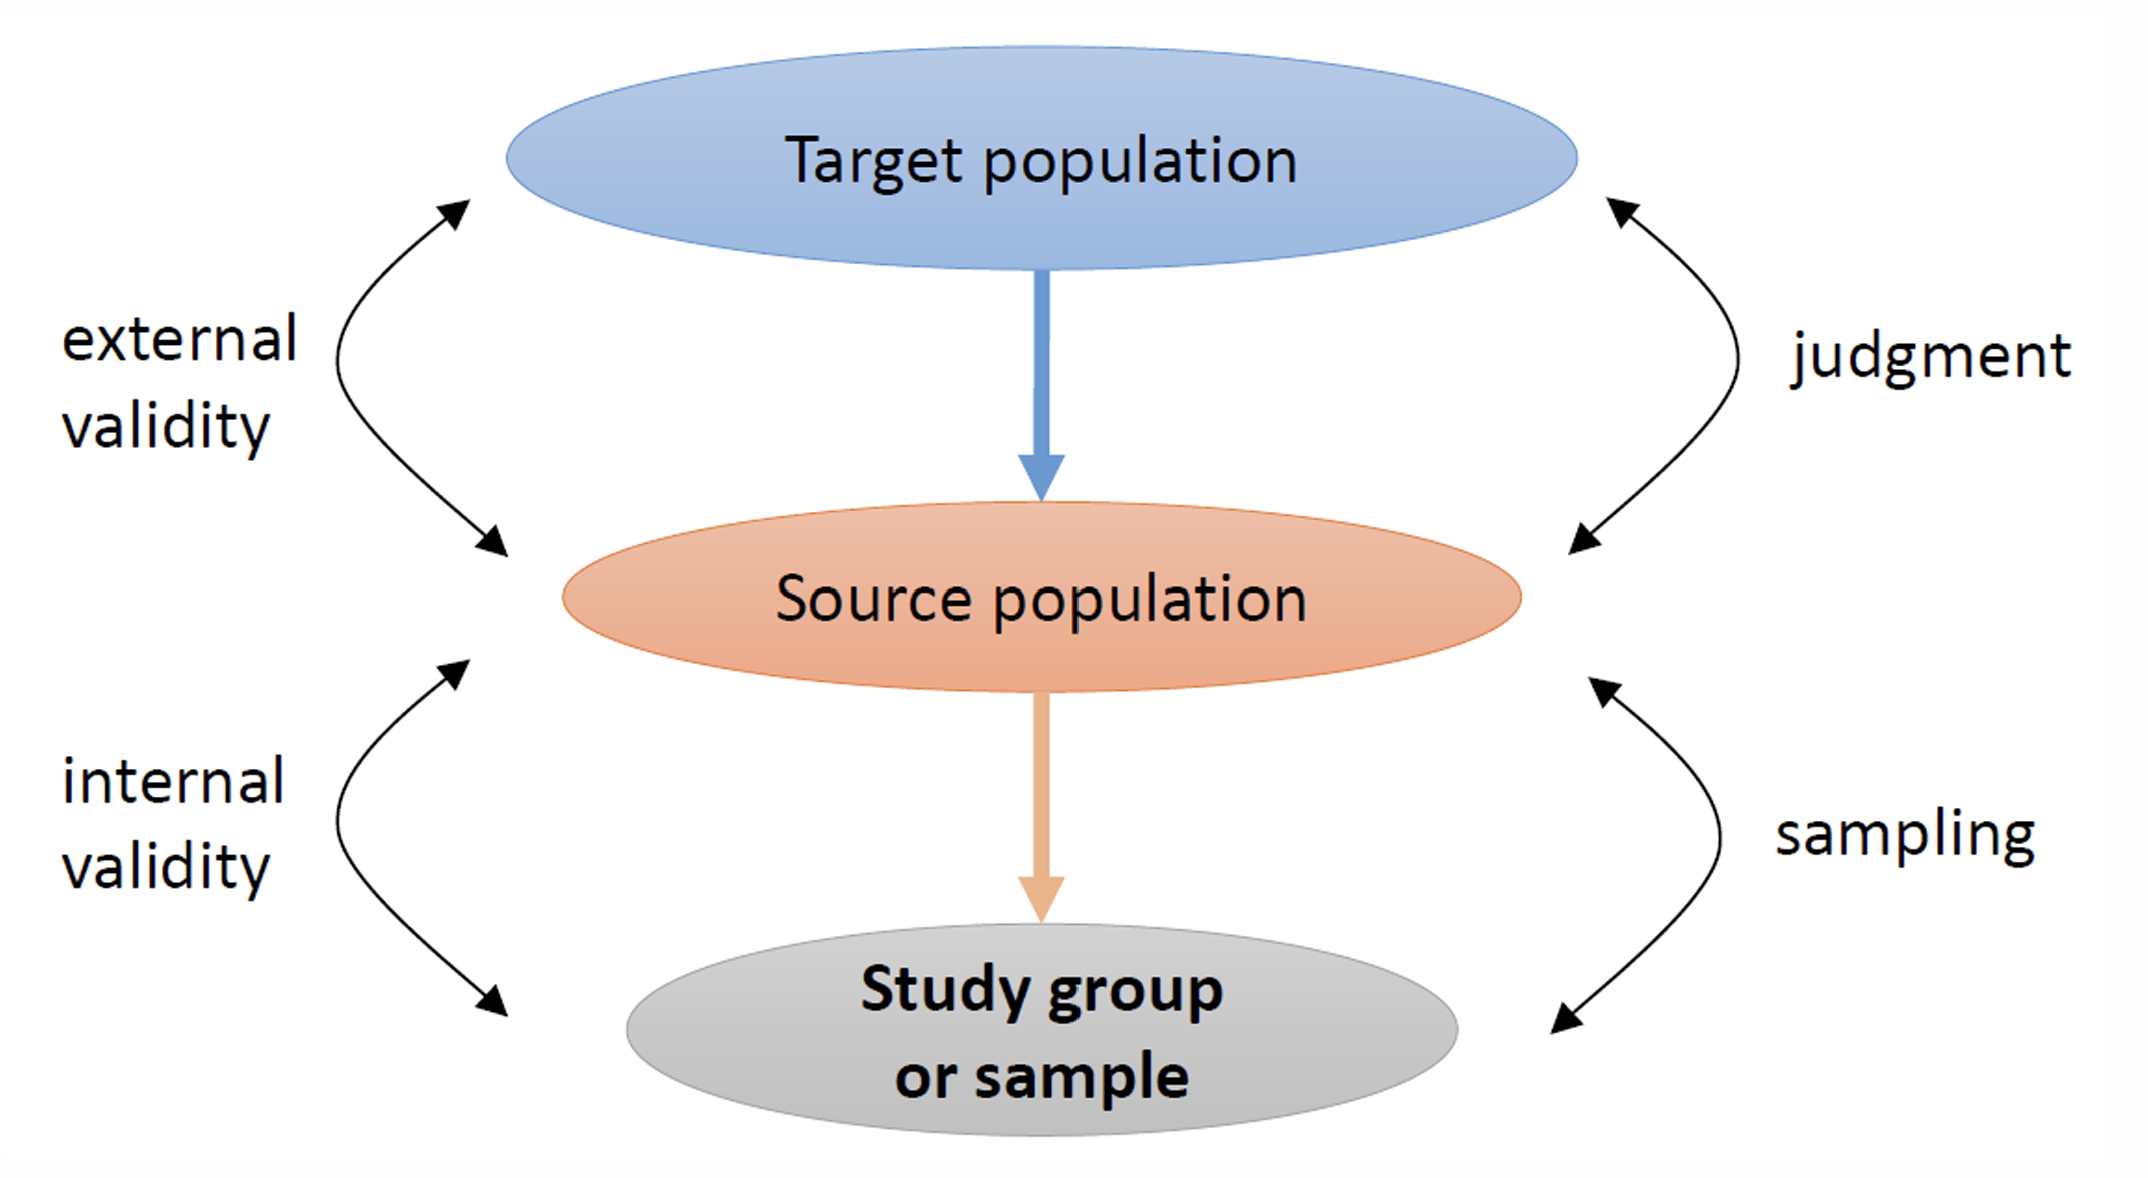
\includegraphics[width=0.8\textwidth]{sampling-method/introduction/population.png}
	\caption{群体} 
\end{figure}

\section{抽样设计}
\begin{center}
	\begin{equation}
		\text{抽样设计}
		\begin{cases}
			\text{概率抽样} 
			\begin{cases}
				\text{简单随机抽样} \\
				\text{分层抽样} \\
				\text{整群抽样} \\
			\end{cases}\\
			\text{非概率抽样}
			\begin{cases}
				\text{方便抽样} \\
				\text{雪球抽样} \\
				\text{判断抽样} \\
			\end{cases}
		\end{cases}\notag
	\end{equation}
\end{center}
\begin{itemize}
	\item 概率抽样样本是随机产生的,非概率抽样样本不是随机产生的。
	\item 非概率抽样无法判断样本是否具备代表性,也就无法确定抽样误差。但在一定程度上可以说明总体的特征。
	\item 方便抽样是选择最容易获得的样本作为研究对象。
	\item 雪球抽样是先选择一个较小的样本,再让这个样本中的样本单元去提供一些样本。
	\item 判断抽样是研究人员从总体中选择自己认为最能代表总体的个体作为样本。
\end{itemize}

\section{抽样框架}
对可以选择作为样本单元的群体单位列出的名册或排序编号,用以确定总体的抽样范围和结构。

\section{抽样调查随机性的来源}
\subsection{基于模型的方法}
绝大多数统计学课程是基于模型的(model-based approch),它将总体看作是背后随机变量的实现,随机性来源于随机变量的取值。
\subsection{基于设计的方法}
抽样调查是基于设计的(design-based approch),它将总体中个体的值看作为定值,而随机性来源于是否抽到该个体。

\section{概率抽样概述}
\subsection{样本概率}
记一个可能的样本为$s$,记在抽样设计下出现这个样本的概率\footnote{样本出现的概率未必是等可能的。}为$p(s)$,应有$\sum\limits_{s}p(s)=1$。
\subsection{入样概率与抽样权重}
对于任意个体$Y_k$,该个体的入样概率$\pi_k$记为$\sum\limits_{Y_k\in s}p(s)$,该个体的抽样权重$w_k$定义为$\frac{1}{\pi_k}$,表示该个体可以代表总体里的多少个个体。若每个个体的抽样权重都一样,则称产生的样本为\gls{SelfWeighting}样本。

%\chapter{简单随机抽样}

简单随机抽样分为\gls{SRS}与\gls{SRSWR}两种。我们通常更喜欢不放回抽样,因为同一个个体在样本中多次出现并不能提供额外的信息,同时有放回抽样会导致估计量的方差更大。\par
简单随机抽样意味着每个样本出现的概率是一样的,即$p(s)$一致,那么每个个体的入样概率也是一致的(样本出现概率一致时每个个体的入样概率服从古典概型)。

\section{SRS的参数估计}

\subsubsection{SRS中$Z$的相关性质} 
\begin{theorem}
	SRS中表示个体是否入样的示性变量具有如下性质:
	\begin{gather*}
		E(Z_i)=\frac{n}{N} \\
		Var(Z_i)=\frac{n}{N}\left(1-\frac{n}{N}\right) \\
		Cov(Z_i,Z_j)=\frac{-n}{N(N-1)}\left(1-\frac{n}{N}\right) 
	\end{gather*}
\end{theorem}
\begin{proof}
	每个个体被抽到的概率为:
	\begin{equation}
		\pi_k=\frac{\binom{N-1}{n-1}}{\binom{N}{n}}=\frac{n}{N}\notag
	\end{equation}      
	由此可知个体示性变量的期望:
	\begin{equation}
		E(Z_i)=1\times P(Z_i=1)=1\times \pi_i=\frac{n}{N}\notag
	\end{equation}
	注意到$E(Z_i^2)=0\times P(Z_i^2=0)+1\times P(Z_i^2=1)=P(Z_i=1)=E(Z_i)$,即有:
	\begin{equation*}
		Var(Z_i)=E(Z_i^2)-E^2(Z_i)
		=E(Z_i)\left(1-E(Z_i)\right)
		=\frac{n}{N}\left(1-\frac{n}{N}\right)
	\end{equation*}
	注意到$E(Z_iZ_j)=P(Z_i=1,\;Z_j=1)$,所以:
	\begin{equation*}
		Cov(Z_i,Z_j)=E(Z_iZ_j)-E(Z_i)E(Z_j)
		=\frac{\binom{N-2}{n-2}}{\binom{N}{n}}-E^2(Z_i)
		=\frac{-n}{N(N-1)}\left(1-\frac{n}{N}\right) \qedhere
	\end{equation*}
\end{proof}

\subsection{SRS总体均值$\mu$的估计} 
\subsubsection{点估计及点估计的性质}
\begin{theorem}
	在SRS中中利用样本均值可对总体均值$\mu$给出如下点估计:
	\begin{equation*}
		\hat{\mu}=\frac{1}{n}\sum\limits_{i=1}^{n}y_i=\frac{1}{n}\sum\limits_{i=1}^{N}Y_iZ_i
	\end{equation*}
	该点估计具有如下性质:
	\begin{gather*}
		E(\hat{\mu})=\mu,\;Var(\hat{\mu})=\left(1-\frac{n}{N}\right)\frac{\sigma^2}{n} \\
		\widehat{Var}(\hat{\mu})=\left(1-\frac{n}{N}\right)\frac{s^2}{n}\text{是关于}Var(\hat{\mu})\text{的无偏估计。}
	\end{gather*}
\end{theorem}
其中方差的计算见下文总体总量方差的推导,由方差的性质即可推导出总体均值的方差。\footnote{$\left(1-\frac{n}{N}\right)$被称之为\gls{FPC},有放回抽样或$N$远大于$n$时不需要FPC。}
\subsubsection{区间估计}
\begin{theorem}
	由大数定律,大样本下有:
	\begin{equation*}
		\frac{\hat{\mu}-\mu}{\sqrt{Var(\hat{\mu})}}\sim N(0,\;1)
	\end{equation*}
	所以SRS中总体均值$\mu$的区间估计如下:
	\begin{equation}
		\hat{\mu}\pm u_{1-\frac{\alpha}{2}}\times\sqrt{Var(\hat{\mu})}\notag
	\end{equation}
	由于$Var(\hat{\mu})$的计算中涉及未知参数$\sigma^2$,以$\widehat{Var}(\hat{\mu})$代替,因此置信度为$(1-\alpha)$的估计的双侧置信区间为\label{sec:SRSmuci}:
	\begin{equation}
		\hat{\mu}\pm u_{1-\frac{\alpha}{2}}\times\sqrt{\widehat{Var}(\hat{\mu})}\notag
	\end{equation}
\end{theorem}

\subsection{SRS总体总量$\tau$的估计}
\subsection*{点估计}
\subsubsection{利用样本均值进行估计}
\begin{definition}
	在SRS中利用样本均值可对总体总量$\tau$给出如下点估计:
	\begin{gather*}
		\hat{\tau}=N\hat{\mu}=\frac{N}{n}\sum\limits_{i=1}^{n}y_i=\frac{N}{n}\sum\limits_{i=1}^{N}Y_iZ_i
	\end{gather*}
\end{definition}
\subsubsection{Horvitz-Thompson估计量(HT估计量)}
\begin{definition}
	在SRS中引入抽样权重可给出关于$\tau$的HT估计:
	\begin{equation*}
		\hat{\tau}=\sum\limits_{i=1}^{n}w_iy_i=\sum\limits_{i=1}^Nw_iY_iZ_i
	\end{equation*}
\end{definition}
\subsubsection{点估计的性质}
\begin{theorem}
	关于SRS总体总量$\tau$的点估计有如下性质:
	\begin{gather*}
		E(\hat{\tau})=\tau \\ Var(\hat{\tau})=N^2\left(1-\frac{n}{N}\right)\frac{\sigma^2}{n},\quad
		\widehat{Var}(\hat{\tau})=N^2\left(1-\frac{n}{N}\right)\frac{s^2}{n}
	\end{gather*}
\end{theorem}
下给出点估计估计量方差公式的证明。
\begin{proof}
	将方差展开可得到:
	\begin{align*}
		Var(\hat{\tau})
		&=Var\left(\sum\limits_{i=1}^Nw_iY_iZ_i\right) \\
		&=\sum\limits_{i=1}^NVar(w_iY_iZ_i)+2\sum\limits_{i=1}^N\sum\limits_{j=i+1}^NCov(w_iY_iZ_i,w_jY_jZ_j) \\
		&=\sum\limits_{i=1}^Nw_i^2Y_i^2Var(Z_i)+2\sum\limits_{i=1}^N\sum\limits_{j=i+1}^Nw_iY_iw_jY_jCov(Z_i,Z_j) \\	
	\end{align*}	
	注意到$w_i=\frac{N}{n}$并代入$Z_i$相关性质的公式可以得到:
	\begin{align*}
		Var(\hat{\tau})
		&=\sum\limits_{i=1}^Nw_i^2Y_i^2Var(Z_i)+2\sum\limits_{i=1}^N\sum\limits_{j=i+1}^Nw_iY_iw_jY_jCov(Z_i,Z_j) \\
		&=\frac{N}{n}\left(1-\frac{n}{N}\right)\frac{1}{N-1}\sum\limits_{i=1}^{N}\left[(N-1)Y_i^2-\sum\limits_{j=i+1}^N2Y_iY_j\right] \\
		&=\frac{N}{n}\left(1-\frac{n}{N}\right)\frac{1}{N-1}\left[\sum\limits_{i=1}^{N}(N-1)Y_i^2-\sum\limits_{i=1}^{N}\sum\limits_{j=i+1}^N2Y_iY_j\right] \\
		&=\frac{N}{n}\left(1-\frac{n}{N}\right)\frac{1}{N-1}\left[\sum\limits_{i=1}^{N}(N-1)Y_i^2-\left(\sum\limits_{i=1}^NY_i\right)^2+\sum\limits_{i=1}^NY_i^2\right] \\
		&=\frac{N}{n}\left(1-\frac{n}{N}\right)\frac{1}{N-1}\left[N\sum\limits_{i=1}^{N}Y_i^2-\left(\sum\limits_{i=1}^NY_i\right)^2\right] \\
		&=\frac{N^2}{n}\left(1-\frac{n}{N}\right)\frac{1}{N-1}\left(\sum\limits_{i=1}^{N}Y_i^2-N\mu^2\right)
	\end{align*}
	\begin{align*}
		Var(\hat{\tau})
		&=\frac{N^2}{n}\left(1-\frac{n}{N}\right)\frac{1}{N-1}\left(\sum\limits_{i=1}^{N}Y_i^2-2N\mu^2+N\mu^2\right) \\
		&=\frac{N^2}{n}\left(1-\frac{n}{N}\right)\frac{1}{N-1}\left(\sum\limits_{i=1}^{N}Y_i^2-2\mu\sum\limits_{i=1}^NY_i+N\mu^2\right) \\     
		&=\frac{N^2}{n}\left(1-\frac{n}{N}\right)\frac{1}{N-1}\sum\limits_{i=1}^N(Y_i-\mu)^2 \\ 
		&=\frac{N^2}{n}\left(1-\frac{n}{N}\right)\sigma^2 \qedhere
	\end{align*}
\end{proof}
\subsection*{区间估计}
\begin{theorem}
	由大数定律,大样本下有:
	\begin{equation}
		\frac{\hat{\tau}-\tau}{\sqrt{Var(\hat{\tau})}}\sim N(0,\;1)\notag
	\end{equation}
	所以SRS中总体总量$\tau$的区间估计如下:
	\begin{equation}
		\hat{\tau}\pm u_{1-\frac{\alpha}{2}}\times\sqrt{Var(\hat{\tau})}\notag
	\end{equation}
	由于$Var(\hat{\tau})$的计算中涉及未知参数$\sigma^2$,以$\widehat{Var}(\hat{\tau})$代替,因此置信度为$(1-\alpha)$的估计的双侧置信区间为:
	\begin{equation}
		\hat{\tau}\pm u_{1-\frac{\alpha}{2}}\times\sqrt{\widehat{Var}(\hat{\tau})}\notag
	\end{equation}
\end{theorem}

\subsection{SRS总体方差$\sigma^2$的估计}
\begin{definition}
	在SRS中利用样本方差可对总体方差$\sigma^2$给出如下点估计:
	\begin{equation}
		\hat{\sigma^2}=s^2=\frac{1}{n-1}\sum\limits_{i=1}^n(y_i-\overline{y})^2=\frac{1}{n-1}\sum\limits_{i=1}^N(Y_i-\hat{\mu})^2Z_i\notag
	\end{equation}
\end{definition}
\section{SRS阳性率问题}
阳性率问题是前述问题的一种特殊形式,$Y_i$只能在$0$和$1$中取值。因此阳性率$p$即为总体均值$\mu$。
\subsection{阳性率$p$的估计}
\subsubsection{点估计}
\begin{definition}
	在SRS中利用样本阳性率可给出阳性率$p$的点估计如下:
	\begin{equation*}
		\hat{p}=\frac{1}{n}\sum\limits_{i=1}^{n}y_i=\frac{1}{n}\sum\limits_{i=1}^{N}Y_iZ_i
	\end{equation*}
	该点估计具有如下性质:
	\begin{gather*}
		E(\hat{p})=p,\quad
		Var(\hat{p})=\left(1-\frac{n}{N}\right)\frac{\sigma^2}{n},\quad
		\widehat{Var}(\hat{p})=\left(1-\frac{n}{N}\right)\frac{s^2}{n}
	\end{gather*}
\end{definition}

\subsubsection{区间估计}
\begin{theorem}
	由大数定律,大样本下有:
	\begin{equation}
		\frac{\hat{p}-p}{\sqrt{Var(\hat{p})}}\sim N(0,\;1)\notag
	\end{equation}
	所以SRS中阳性率$p$的区间估计如下:
	\begin{equation}
		\hat{p}\pm u_{1-\frac{\alpha}{2}}\sqrt{Var(\hat{p})}\notag
	\end{equation}
	由于$Var(\hat{p})$的计算中涉及未知参数$\sigma^2$,以$\widehat{Var}(\hat{p})$代替,因此置信度为$(1-\alpha)$的估计的双侧置信区间为:
	\begin{equation}
		\hat{p}\pm u_{1-\frac{\alpha}{2}}\sqrt{\widehat{Var}(\hat{p})}\notag
	\end{equation}
	上述计算公式需要满足$n\hat{p}\geqslant5$和$n(1-\hat{p})\geqslant 5$,即大样本条件。
\end{theorem}

\subsection{总体方差$\sigma^2$的估计}
\subsubsection{总体方差$\sigma^2$与总体均值$p$的关系}
由于$Y_i^2=Y_i$,可得:
\begin{equation}
	\sigma^2=\frac{1}{N-1}\sum_{i=1}^N(Y_i-p)^2=\frac{N}{N-1}p(1-p)\notag
\end{equation}
\subsubsection{点估计}
\begin{definition}
	在SRS中利用样本方差可对总体方差$\sigma^2$给出如下点估计:
	\begin{equation}
		\hat{\sigma^2}=s^2=\frac{1}{n-1}\sum_{i=1}^n(y_i-\overline{y})^2=\frac{1}{n-1}\sum_{i=1}^n(y_i-\hat{p})^2=\frac{n}{n-1}\hat{p}(1-\hat{p})\notag
	\end{equation}
\end{definition}


\section{SRSWR的参数估计}
\subsubsection{SRSWR中$Q$的相关性质}
\begin{theorem}
	SRSWR中表示个体在样本中出现次数的变量$Q_i$具有如下性质:
	\begin{gather*}
		\overrightarrow{Q}=(Q_1,Q_2,\dots,Q_N)\sim \text{Multi}\left(n,\; \overbrace{\left(\frac{1}{N},\;\frac{1}{N},\dots,\frac{1}{N}\right)}^{\text{N个}\;\frac{1}{N}}\right)\\
		Q_i\sim\text{Binom}\left(n,\;\frac{1}{N}\right) \\
		E(Q_i)=\frac{n}{N},\;Var(Q_i)=\frac{n}{N}\left(1-\frac{1}{N}\right) ,\;Cov(Q_i,\;Q_j)=-\frac{n}{N^2}
	\end{gather*}
\end{theorem}
\begin{proof} 
	由多项分布性质:多项分布随机变量的一维边际分布是二项分布,因此上第二、三式成立。下证第四式,将$Q_i$分解为独立二项分布随机变量的和,有:
	\begin{align*}
		Cov(Q_i,\;Q_j)&=Cov\left[\sum_{k=1}^nI_i(k),\;\sum_{l=1}^nI_j(l)\right] \\
		&=\sum_{k=1}^n\sum_{l=1}^nCov[I_i(k),\;I_j(l)] \\
		&=\sum_{k=l}Cov[I_i(k),\;I_j(l)]+\sum_{k\ne l}Cov[I_i(k),\;I_j(l)]
	\end{align*}
	由二项分布随机变量的独立性,后一项为$0$:
	\begin{equation*}
		Cov(Q_i,\;Q_j)
		=\sum_{k=1}^nCov[I_i(k),\;I_j(k)] =\sum_{k=1}^n\left\{E[I_i(k)I_j(k)]-E[I_i(k)]E[I_j(k)]\right\}
	\end{equation*}
	由于同一次伯努利实验中不可能出现两个结果,所以前一项为$0$:
	\begin{equation*}
		Cov(Q_i,\;Q_j)
		=-\sum_{k=1}^nE[I_i(k)]E[I_j(k)]
		=-np_ip_j
		=-\frac{n}{N^2} \qedhere
	\end{equation*}
\end{proof}

\subsection{SRSWR总体总量$\tau$的估计}
\begin{theorem}
	在SRS中中利用样本均值可对总体总量$\tau$给出如下点估计:
	\begin{equation*}
		\hat{\tau}=\frac{N}{n}\sum_{i=1}^NY_iQ_i
	\end{equation*}
	该点估计具有如下性质:
	\begin{equation*}
		E(\hat{\tau})=\tau,\;Var(\hat{\tau})=\frac{N(N-1)}{n}\sigma^2
	\end{equation*}
\end{theorem}
\begin{proof}
	将方差展开可得到:
	\begin{align*}
		Var(\hat{\tau})
		&=Var\left(\frac{N}{n}\sum_{i=1}^N Q_iY_i\right) \\
		&=\frac{N^2}{n^2}\left[\sum_{i=1}^{N}Y_i^2 Var(Q_i)+2\sum_{i=1}^N\sum_{j=i+1}^NY_iY_j Cov(Q_i, Q_j)\right] \\
		&=\frac{N^2}{n^2}\left[\sum_{i=1}^{N}Y_i^2\frac{n}{N}\left(1-\frac{1}{N}\right)+2\sum_{i=1}^N\sum_{j=i+1}^NY_iY_j \frac{-n}{N^2}\right] \\
		&=\frac{N}{n}\left[\sum_{i=1}^{N}Y_i^2\left(1-\frac{1}{N}\right)-\frac{1}{N}\sum_{i=1}^N\sum_{j=i+1}^N2Y_iY_j\right]
	\end{align*}
	此处使用平方和公式(该技巧常用):
	\begin{align*}
		Var(\hat{\tau})
		&=\frac{N}{n}\left\{\sum_{i=1}^{N}Y_i^2\left(1-\frac{1}{N}\right)-\frac{1}{N}\left[\left(\sum_{i=1}^NY_i\right)^2-\sum_{i=1}^NY_i^2\right]\right\} \\
		&=\frac{N}{n}\left[\sum_{i=1}^{N}Y_i^2-\frac{1}{N}\left(\sum_{i=1}^NY_i\right)^2\right]
	\end{align*}
	此处使用$N\mu^2$并进行加减凑项(该技巧常用):
	\begin{equation*}
		Var(\hat{\tau})          =\frac{N}{n}\left(\sum_{i=1}^{N}Y_i^2-N\mu^2\right)
		=\frac{N}{n}\left(\sum_{i=1}^{N}Y_i^2-2N\mu^2+N\mu^2\right)
	\end{equation*}
	此处使用$N\mu=\sum\limits_{i=1}^NY_i$(该技巧常用):
	\begin{equation*}
		Var(\hat{\tau}) =\frac{N}{n}\left(\sum_{i=1}^{N}Y_i^2-2\mu\sum_{i=1}^NY_i+N\mu^2\right)
		=\frac{N}{n}\sum_{i=1}^N(Y_i-\mu)^2
		=\frac{N(N-1)}{n}\sigma^2 \qedhere
	\end{equation*}
\end{proof}

\section{样本容量的选择}
抽样分布的方差决定置信区间的长度,样本容量增大的时候抽样分布的方差减小,置信区间变窄。
\subsubsection{注意事项}
通过控制总体均值的置信区间长度去选择样本容量而不从总体总量来考虑,因为总体总量的方差计算中还会涉及到$N^2$,这对于无穷总体是无法进行计算的。无穷总体时忽略被FPC。
\subsubsection{误差幅度MOE}
置信区间的半径称之为\gls{MOE}。

\subsection{总体均值样本容量公式}
\begin{theorem}
	待估参数为总体均值时有如下样本容量公式:
	\begin{equation}
		n_{\text{SRS}}=\frac{1}{\frac{d^2}{u^2\sigma^2}+\frac{1}{N}},\quad n_{\text{SRSWR}}=\frac{u^2\sigma^2}{d^2}\notag
	\end{equation}
	其中$u$为求解区间估计过程中选择的正态分布分位数。\par
	上式中二者有关系(又称为两步法):
	\begin{equation}
		\frac{1}{n_{\text{SRS}}}=\frac{1}{n_{\text{SRSWR}}}+\frac{1}{N}\notag
	\end{equation}
\end{theorem}
公式涉及到总体方差真实值$\sigma^2$,解决方案:
\begin{enumerate}
	\item 使用历史数据的样本方差代替$\sigma^2$。
	\item 由正态分布的性质,在$\mu\pm2\sigma$范围内应包含了$97.7\%$的样本,因此,我们使用样本的极差来近似$4\sigma$:用样本极差除4替代$\sigma$。但是这个时候又涉及到极差从何而来的问题,因为是先确定样本容量再去做抽样,没有样本怎么来的极差呢?查阅资料得到样本的大致分布范围。
\end{enumerate}

\subsection{总体阳性率样本容量公式}
\begin{theorem}
	待估参数为总体阳性率时有如下样本容量公式:
	\begin{equation}
		n_{SRS}=\frac{Np(1-p)}{\frac{d^2}{u^2}(N-1)+p(1-p)},\quad n_{\text{SRSWR}}=\frac{u^2p(1-p)}{d^2}\notag
	\end{equation}
	其中$u$为求解区间估计过程中选择的正态分布分位数。
\end{theorem}
但这里需要注意,阳性率问题两步法不能用,与理论公式不等。\par
公式涉及到阳性率的真实值$p$,解决方法:
\begin{enumerate}
	\item 有根据的推测,使用历史数据来替代真实阳性率。
	\item 取$p=0.5$,最大化样本容量,进行保守估计。
	\item 如果获取额外样本的代价大于开始一次抽样的代价(也就意味着最大化样本容量带来的代价大于去做一次抽样来估计一下真实值的代价),那在没有历史数据的情况下可以自己去抽样。
\end{enumerate}
\subsubsection{阳性率问题下理论公式难以推导的情况}
蒙特卡罗,代码如下:
\inputminted[bgcolor=white, linenos, frame=single, numbersep=5pt, breaklines]{r}{sampling-method/SRS/sample_size_p.R}
\section{简单随机抽样适用条件}
\begin{enumerate}
	\item 可使用的额外信息较少。
	\item 研究多元关系,没有特别特殊的理由使用别的抽样方法。
\end{enumerate}


%\chapter{回归估计与比例估计}

本章介绍\gls{RegEstimate}与\gls{RatioEstimate},回归估计认为个体值$y$与某个变量$x$(即\gls{AuxiliaryVariable})之间存在如下关系:
\begin{equation*}
	y=B_1x+B_0
\end{equation*}
比例估计中取$B_0=0$,因此它可以看作为回归估计的一个特例。先来介绍辅助变量。

\section{辅助变量}
在回归估计中我们通过辅助变量去得到我们想要的估计值。

\subsection{辅助变量选择要求}
辅助变量需要满足以下条件:
\begin{enumerate}
	\item 辅助变量的获得需要简单快捷。如果它的值都很难得到或者得不到那根本没办法作回归估计。
	\item 辅助变量需要和个体值之间存在高度的线性相关性,在比例估计中我们还要求二者线性方程中的截距为$0$(如果存在截距那截距就会是一个偏倚)。
\end{enumerate}
\hspace{2em}选择好辅助变量并获取数据后,可以去做辅助变量与样本单元值的线性回归,来检验是否满足高度线性相关性(这里其实假设了数据满足正态分布)。在比例估计中我们还要去检验截距是否为$0$。如果线性回归后的截距很小但不显著,我们可以认为满足要求;如果截距较大但不显著,我们认为是样本随机性带来的问题,可以认为截距满足为$0$的条件。\par


\subsection{辅助变量与个体值的相关性}
\begin{theorem}
	对于辅助变量与个体值的相关性,有如下结论:
	\begin{equation}
		Corr(\bar{x},\bar{y})=Corr(X,Y)\notag
	\end{equation}
\end{theorem}
\begin{proof}
	将协方差进行展开:
	\begin{align*}
		Cov(\bar{x},\bar{y})
		&=Cov\left(\frac{1}{n}\sum_{i=1}^NX_iZ_i,\frac{1}{n}\sum_{j=1}^NY_jZ_j\right) \\
		&=\frac{1}{n^2}\left[\sum_{i=1}^NX_iY_iVar(Z_i)+2\sum_{i=1}^N\sum_{j\ne i}^NX_iY_jCov(Z_i,Z_j)\right] \\
		&=\left(1-\frac{n}{N}\right)\frac{1}{nN}\frac{1}{N-1}\left[(N-1)\sum_{i=1}^NX_iY_i-\sum_{i=1}^N\sum_{j\ne i}^NX_iY_j\right] \\
		&=\left(1-\frac{n}{N}\right)\frac{1}{nN}\frac{1}{N-1}\left[(N-1)\sum_{i=1}^NX_iY_i-\left(\sum_{i=1}^N\sum_{j=1}^NX_iY_j-\sum_{i=1}^NX_iY_i\right) \right] \\
		&=\left(1-\frac{n}{N}\right)\frac{1}{nN}\frac{1}{N-1}\left(N\sum_{i=1}^NX_iY_i-\sum_{i=1}^N\sum_{j=1}^NX_iY_j\right) \\
		&=\left(1-\frac{n}{N}\right)\frac{1}{nN}\frac{1}{N-1}\left(N\sum_{i=1}^NX_iY_i-\sum_{i=1}^NX_i\sum_{j=1}^NY_j\right) \\
		&=\left(1-\frac{n}{N}\right)\frac{1}{n}\frac{1}{N-1}\left(\sum_{i=1}^NX_iY_i-N\mu_X\mu_Y\right) \\
		&=\left(1-\frac{n}{N}\right)\frac{1}{n}\frac{1}{N-1}\left(\sum_{i=1}^NX_iY_i-2N\mu_X\mu_Y+N\mu_X\mu_Y\right) \\
		&=\left(1-\frac{n}{N}\right)\frac{1}{n}\frac{1}{N-1}\left(\sum_{i=1}^NX_iY_i-\sum_{i=1}^NX_i\mu_Y-\sum_{i=1}^NY_i\mu_X+N\mu_X\mu_Y\right) \\
		&=\left(1-\frac{n}{N}\right)\frac{1}{n}\frac{1}{N-1}\sum_{i=1}^N(X_iY_i-X_i\mu_Y-Y_i\mu_X+\mu_X\mu_Y) \\
		&=\left(1-\frac{n}{N}\right)\frac{1}{n}\frac{\sum_{i=1}^N(X_iY_i-X_i\mu_Y-Y_i\mu_X+\mu_X\mu_Y)}{N-1} \\
		&=\left(1-\frac{n}{N}\right)\frac{1}{n}\frac{\sum_{i=1}^N(X_i-\mu_X)(Y_i-\mu_Y)}{N-1} \\
		&=\left(1-\frac{n}{N}\right)\frac{1}{n}Cov(X,Y)
	\end{align*}
	所以:
	\begin{align*}
		Corr(\bar{x},\bar{y})&=\frac{Cov(\bar{x},\bar{y})}{\sqrt{Var(\bar{x})Var(\bar{y})}} \\
		&=\frac{(1-\frac{n}{N})\frac{1}{n}Cov(X,Y)}{\sqrt{(1-\frac{n}{N})^2\frac{1}{n^2}Var(X)Var(Y)}} \\
		&=\frac{Cov(X,Y)}{\sqrt{Var(X)Var(Y)}} \\
		&=Corr(X,Y) \qedhere
	\end{align*}
\end{proof}
\section{估计量}

\subsection{回归估计量}
\begin{definition}
	比例估计量有如下计算公式(其中$\mu_X$和$\tau_X$是已知的):
	\begin{gather*}
		\hat{B}_1=\frac{\sum\limits_{i=1}^n(x_i-\bar{x})(y_i-\bar{y})}{\sum\limits_{i=1}^n(x_i-\bar{x})^2}=\frac{s_y\hat{R}}{s_x},\quad
		\hat{B}_0=\bar{y}-\hat{B}_1\bar{x} \\
		\hat{\mu}_{Y_{reg}}=\hat{B}_1\mu_X+\hat{B}_0=\hat{B}_1(\mu_X-\bar{x})+\bar{y},\quad
		\hat{\tau}_{Y_{reg}}=\hat{B}_1\tau_X+\hat{B}_0
	\end{gather*}
\end{definition}


\subsection{比例估计量}
\begin{definition}
	比例估计量有如下计算公式(其中$\mu_X$和$\tau_X$是已知的):
	\begin{gather*}
		\hat{B}=\frac{\bar{y}}{\bar{x}}=\frac{\tau_y}{\tau_x} \\
		\hat{\mu}_{Yr}=\hat{B}\mu_X,\quad\hat{\tau}_{Yr}=\hat{B}\tau_X 
	\end{gather*}
\end{definition}
其中$\hat{B}$是比例系数$B$的估计\footnote{这是一个有偏估计!!!},对于$B$的真实值,应有$B=\frac{\mu_Y}{\mu_X}=\frac{\tau_Y}{\tau_X}$。\footnote{依据辅助变量的选择原则,$X$与$Y$之间需要满足线性关系且截距为$0$,$B$其实就是线性关系中的斜率,同时证明了$Corr(\bar{x},\bar{y})=Corr(X,Y)$,因此$\hat{B}$和$B$既可以由均值来表示也可以由总体总量来表示。}
\section{偏差}
\subsection{回归估计的偏差}
由回归估计量计算公式显然可知回归估计是有偏的。
\subsection{比例估计的偏差}
\begin{theorem}
	比例估计量是有偏的,偏差如下:
	\begin{gather*}
		bias(\hat{\mu}_{Yr})=E(\hat{\mu}_{Yr})-\mu_Y=Cov(-\hat{B},\bar{x}) \\
		bias(\hat{\tau}_{Yr})=E(\hat{\tau}_{Yr})-\tau_Y=Cov(-\hat{B},\bar{x})N
	\end{gather*}
	上式不便于计算,可以用下式进行估计:
	\begin{gather*}
		bias(\hat{\mu}_{Yr})\approx\frac{1}{\mu_X}\left[BVar(\bar{x})-Cov(\bar{x},\bar{y})\right]=\left(1-\frac{n}{N}\right)\frac{1}{n\mu_X}[B\sigma_X^2-Corr(X,Y)\sigma_X\sigma_Y] \\
		bias(\hat{\tau}_{Yr})\approx\frac{\tau_X}{\mu_X^2}\left[BVar(\bar{x})-Cov(\bar{x},\bar{y})\right]=\left(1-\frac{n}{N}\right)\frac{\tau_X}{n\mu_X^2}[B\sigma_X^2-Corr(X,Y)\sigma_X\sigma_Y]
	\end{gather*}
\end{theorem}
\begin{proof}
	将协方差分解:
	\begin{align*}
		Cov(-\hat{B},\bar{x})&=-Cov(\hat{B},\bar{x}) \\
		&=-\left[E(\hat{B}\bar{x})-E(\hat{B})E(\bar{x})\right] \\
		&=-\left[E\left(\frac{\bar{y}}{\bar{x}}\bar{x}\right)-E(\hat{B})\mu_X\right] \\
		&=E(\hat{\mu}_{Yr})-E(\bar{y}) \\
		&=E(\hat{\mu}_{Yr})-\mu_Y
	\end{align*}
	下证近似公式:
	\begin{align*}
		bias(\hat{\mu}_{Yr})
		&=E(\hat{B}\mu_X)-\mu_Y \\
		&=\mu_XE\left(\frac{\bar{y}}{\bar{x}}-\frac{\mu_Y}{\mu_X}\right) \\
		&=\mu_XE\left(\frac{\bar{y}}{\mu_X}\frac{\mu_X}{\bar{x}}-\frac{\mu_Y}{\mu_X}\right) \\
		&=\mu_XE\left(\frac{\bar{y}}{\mu_X}-\frac{\bar{y}}{\mu_X}\frac{\bar{x}-\mu_X}{\bar{x}}-\frac{\mu_Y}{\mu_X}\right) \\
		&=\mu_XE\left(\frac{\bar{y}}{\mu_X}\frac{\mu_X-\bar{x}}{\bar{x}}\right) \\
		&=\mu_XE\left(\frac{\bar{y}}{\mu_X}\frac{\mu_X-\bar{x}}{\bar{x}}\frac{\mu_X}{\bar{x}}\frac{\bar{x}}{\mu_X}\right) \\
		&=\mu_XE\left[\frac{\bar{y}}{\mu_X^2}(\mu_X-\bar{x})\frac{\mu_X}{\bar{x}}\right] \\
		&=\mu_XE\left[\frac{\bar{y}}{\mu_X^2}(\mu_X-\bar{x})\left(1-\frac{\bar{x}-\mu_X}{\bar{x}}\right)\right] \\
		&=\mu_XE\left\{\frac{\bar{y}}{\mu_X^2}\left[(\mu_X-\bar{x})+\frac{(\bar{x}-\mu_X)^2}{\bar{x}}\right]\right\} \\
		&=\mu_XE\left[\frac{-\bar{y}(\bar{x}-\mu_X)}{\mu_X^2}+\frac{\bar{y}(\bar{x}-\mu_X)^2}{\mu_X^2\bar{x}}\right] \\
		&=\frac{1}{\mu_X}E\left[\frac{\bar{x}}{\bar{y}}(\bar{x}-\mu_X)^2-(\bar{x}-\mu_X)\bar{y}\right] \\
		&=\frac{1}{\mu_X}\left\{E[\hat{B}(\bar{x}-\mu_X)^2]-E[\bar{y}(\bar{x}-\mu_X)]\right\} \\
		&=\frac{1}{\mu_X}\left\{E[(\hat{B}-B+B)(\bar{x}-\mu_X)^2]-Cov(\bar{x},\bar{y})\right\} \\
		&=\frac{1}{\mu_X}\left\{E[(\hat{B}-B)(\bar{x}-\mu_X)^2+B(\bar{x}-\mu_X)^2]-Cov(\bar{x},\bar{y})\right\}
	\end{align*}
	由于$E\left[(\hat{B}-B)(\bar{x}-\mu_X)^2\right]$极小(严谨证明不提供),因此:
	\begin{align*}
		bias(\hat{\mu}_{Yr})&\approx\frac{1}{\mu_X}\left\{E[B(\bar{x}-\mu_X)^2]-Cov(\bar{x},\bar{y})\right\} \\
		&=\frac{1}{\mu_X}\left[BVar(\bar{x})-Cov(\bar{x},\bar{y})\right] \qedhere
	\end{align*}
\end{proof}
由此,在以下情况比例估计的偏倚会较小:
\begin{enumerate}
	\item n较大。
	\item $\frac{n}{N}$较大。
	\item $\mu_X$较大。
	\item $\sigma_x$较小。
	\item $R$接近$\pm 1$。
\end{enumerate}
\section{均方误差}

\subsection{回归估计量的均方误差}
\begin{theorem}
	回归估计量的均方误差为:
	\begin{align*}
		MSE(\hat{\mu}_{Y_{reg}})&= 
		E\left\lbrace\big[\bar{y}+\hat{B}_1(\mu_X-\bar{x})-\mu_Y\big]^2\right\rbrace  \\
		&\approx Var(\bar{d}) \\
		&=\left(1-\frac{n}{N}\right)\frac{\sigma_d^2}{n}
	\end{align*}
	其中:
	\begin{gather*}
		d_i=y_i-\big[\mu_Y+B_1(x_i-\mu_X)\big] \\
		\sigma_d^2=\frac{1}{N-1}\sum_{i=1}^N[y_i-\mu_Y-B_1(x_i-\mu_X)]^2=(1-R^2)\sigma_Y^2
	\end{gather*}
\end{theorem}
\begin{proof}
	下求$E(d)$:
	\begin{equation*}
		E(d)=\frac{1}{N}\left[\sum_{i=1}^Ny_i-N\mu_Y-B_1\sum_{i=1}^Nx_i+B_1N\mu_X\right]=0
	\end{equation*}
	因此:
	\begin{align*}
		\sigma_d^2&=\frac{1}{N-1}\sum_{i=1}^N\big[y_i-\mu_Y-B_1(x_i-\mu_X)\big]^2 \\
		&=\frac{1}{N-1}\left[\sum_{i=1}^N(y_i-\mu_Y)^2+\sum_{i=1}^NB_1^2(x_i-\mu_X)^2-\sum_{i=1}^N2B_i(y_i-\mu_Y)(x_i-\mu_X)\right] \\
		&=\sigma_Y^2+B_1^2\sigma_X^2-2B_1R\sigma_X\sigma_Y
	\end{align*}
	而:
	\begin{equation*}
		B_1=\frac{\sigma_YR}{\sigma_X}
	\end{equation*}
	所以:
	\begin{equation*}
		\sigma_d^2
		=\sigma_Y^2+B_1^2\sigma_X^2-2B_1R\sigma_X\sigma_Y 
		=\sigma_Y^2+\frac{\sigma_Y^2R^2}{\sigma_X^2}\sigma_X^2-2\frac{\sigma_YR}{\sigma_X}R\sigma_X\sigma_Y
		=\sigma_Y^2-R^2\sigma_Y^2
		=(1-R^2)\sigma_Y^2\qedhere
	\end{equation*}
\end{proof}
由此,在以下情况$MSE(\hat{\mu}_{Y_{reg}})$较小:
\begin{enumerate}
	\item $n$较大。
	\item $\frac{n}{N}$较大。
	\item $\sigma_Y$较小。
	\item $R$接近$\pm 1$。
\end{enumerate}


\subsection{比例估计量的均方误差}
\begin{theorem}
	比例估计量的均方误差为:
	\begin{align*}
		MSE(\hat{\mu}_{Yr})&\approx E\left[(\bar{y}-B\bar{x})^2\right] \\
		&=\left(1-\frac{n}{N}\right)\frac{\sigma_Y^2-2BR\sigma_X\sigma_Y+B^2\sigma_X^2}{n} \\
		&\approx Var(\hat{\mu}_{Yr})
	\end{align*}
\end{theorem}
证明过程可见David and Sukhatme, 1974。


\section{方差}
\subsection{回归估计的方差}
\begin{theorem}
	回归估计的方差为:
	\begin{equation*}
		Var(\hat{\mu}_{Y_{reg}})=Var(\bar{d})=\left(1-\frac{n}{N}\right)\frac{\sigma_d^2}{n}=\left(1-\frac{n}{N}\right)\frac{(1-R^2)\sigma_Y^2}{n}
	\end{equation*}
\end{theorem}
定义$e_i=y_i-(\hat{B}_1x_i+\hat{B}_0)$可得:
\begin{equation*}
	\widehat{Var}(\hat{\mu}_{Y_{reg}})=\left(1-\frac{n}{N}\right)\frac{s_e^2}{n}
\end{equation*}
这里$s_e^2$可取两种计算公式:
\begin{equation*}
	s_e^2=\frac{1}{n-1}\sum_{i=1}^ne_i^2=\left(1-\frac{n}{N}\right)\frac{(1-\hat{R}^2)s_y^2}{n},\quad
	s_e^2=\frac{1}{n-2}\sum_{i=1}^ne_i^2
\end{equation*}
第二种是考虑回归估计有两个待估参数,自由度为$n-2$,这样子做修正了回归中自由度的问题。\par
由上述总结:
\begin{gather*}
	\widehat{Var_1}(\hat{\mu}_{Y_{reg}})=\left(1-\frac{n}{N}\right)\frac{1}{n}\frac{1}{n-1}\sum_{i=1}^n\left[y_i-(\hat{B}_1x_i+\hat{B}_0)\right]^2 \\
	\widehat{Var_2}(\hat{\mu}_{Y_{reg}})=\left(1-\frac{n}{N}\right)\frac{1}{n}\frac{1}{n-2}\sum_{i=1}^n\left[y_i-(\hat{B}_1x_i+\hat{B}_0)\right]^2 
\end{gather*}

\subsection{比例估计的方差}
由Delta method(见\cref{sec:deltamethod}),注意到关系:
\begin{gather*}
	\hat{B}=\frac{\bar{y}}{\bar{x}}=g(\bar{x},\bar{y}) \\
	\hat{\mu}_{Yr}=\hat{B}\mu_X=g(\hat{B}) \\
	\hat{\tau}_{Yr}=\hat{\mu}_{Yr}\frac{\tau_X}{\mu_X}=\hat{\mu}_{Yr}N
\end{gather*}
可得以下比例估计量的近似方差($R=Corr(X,Y)$):
\begin{gather*}
	Var(\hat{B})\approx\left(1-\frac{n}{N}\right)\frac{\sigma_Y^2-2BR\sigma_X\sigma_Y+B^2\sigma_X^2}{n\mu_X^2}=\left(1-\frac{n}{N}\right)\frac{\sigma_\varepsilon^2}{n\mu_X^2} \\
	\widehat{Var}(\hat{B})\approx\left(1-\frac{n}{N}\right)\frac{s_y^2-2\hat{B}\hat{R}s_xs_y+\hat{B}^2s_x^2}{n\bar{x}^2}=\left(1-\frac{n}{N}\right)\frac{s_e^2}{n\bar{x}^2} \\
	Var(\hat{\mu}_{Yr})\approx\left(1-\frac{n}{N}\right)\frac{\sigma_Y^2-2BR\sigma_X\sigma_Y+B^2\sigma_X^2}{n}=\left(1-\frac{n}{N}\right)\frac{\sigma_\varepsilon^2}{n}  \\
	\widehat{Var_1}(\hat{\mu}_{Yr})\approx\left(1-\frac{n}{N}\right)\frac{s_y^2-2\hat{B}\hat{R}s_xs_y+\hat{B}^2s_x^2}{n}=\left(1-\frac{n}{N}\right)\frac{s_e^2}{n}  \\
	Var(\hat{\tau}_{Yr})\approx N\left(N-n\right)\frac{\sigma_Y^2-2BR\sigma_X\sigma_Y+B^2\sigma_X^2}{n}=N(N-n)\frac{\sigma_\varepsilon^2}{n} \\
	\widehat{Var_1}(\hat{\tau}_{Yr})\approx N(N-n)\frac{s_y^2-2\hat{B}\hat{R}s_xs_y+\hat{B}^2s_x^2}{n}=N(N-n)\frac{s_e^2}{n}
\end{gather*}
再给出第二种总体均值、总体总量比例估计量抽样分布方差的估计:
\begin{gather*}
	\widehat{Var_2}(\hat{\mu}_{Yr})=\widehat{Var}(\hat{B}\mu_X)=\widehat{Var}(\hat{B})\mu_X^2\approx\left(1-\frac{n}{N}\right)\left(\frac{\mu_X}{\bar{x}}\right)^2\frac{s_e^2}{n} \\
	\widehat{Var_2}(\hat{\tau}_{Yr})\approx N(N-n)\left(\frac{\mu_X}{\bar{x}}\right)^2\frac{s_e^2}{n} 
\end{gather*}
下给出上述公式中所有等式的推导。
\begin{proof}
	从模型的角度,根据MSE的估计来看(最后一行是使用了SRS均值的方差公式):
	\begin{gather*}
		\begin{aligned}
			Var(\hat{\mu}_{Yr})&\approx MSE(\hat{\mu}_{Yr})
			\approx E\left[(\bar{y}-B\bar{x})^2\right] \\
			&=E\left[\left(\frac{1}{n}\sum_{i=1}^ny_i-B\frac{1}{n}\sum_{i=1}^nx_i\right)^2\right] \\
			&=E\left\{\left[\frac{1}{n}\sum_{i=1}^n(y_i-Bx_i)\right]^2\right\}
		\end{aligned} \\
		\varepsilon_i=y_i-Bx_i,\;\mu_\varepsilon=E(\varepsilon_i)=0 \\
		\begin{aligned}
			Var(\hat{\mu}_{Yr})
			&\approx E\left\{\left[\frac{1}{n}\sum_{i=1}^n(y_i-Bx_i)\right]^2\right\} \\
			&=E\left[(\bar{\varepsilon})^2\right] \\
			&=E\left[(\bar{\varepsilon}-0)^2\right] \\
			&=E\left[(\bar{\varepsilon}-\mu_\varepsilon)^2\right] \\
			&=Var(\bar{\varepsilon}) \\
			&=\left(1-\frac{n}{N}\right)\frac{\sigma_\varepsilon^2}{n}
		\end{aligned}
	\end{gather*}
	对于$\sigma_\varepsilon^2$:
	\begin{align*}
		\sigma_\varepsilon^2
		&=\frac{1}{N-1}\left[\sum_{i=1}^Ny_i^2+B^2\sum_{i=1}^Nx_i^2-2B\sum_{i=1}^Nx_iyi\right] \\
		&=\frac{1}{N-1}\left[\sum_{i=1}^N(y_i-\mu_Y+\mu_Y)^2+B^2\sum_{i=1}^N(x_i-\mu_X+\mu_X)^2-2B\sum_{i=1}^Nx_iyi\right] \\
		&=\frac{1}{N-1}\left[\sum_{i=1}^N(y_i-\mu_Y)^2+2\sum_{i=1}^N(y_i-\mu_Y)\mu_Y+N\mu_Y^2\right.\\
		&\left.\qquad+B^2\sum_{i=1}^N(x_i-\mu_X)^2+2B^2\sum_{i=1}^N(x_i-\mu_X)\mu_X+B^2N\mu_X^2-2B\sum_{i=1}^Nx_iy_i\right] \\
		&=\sigma_Y^2+B^2\sigma_X^2+\frac{1}{N-1}\left[N\mu_Y^2+B^2N\mu_X^2-2B\sum_{i=1}^Nx_iy_i\right] \\
		&=\sigma_Y^2+B^2\sigma_X^2+\frac{1}{N-1}\left[N\mu_Y^2+B^2N\mu_X^2-2B\sum_{i=1}^N(x_i-\mu_X+\mu_X)(y_i-\mu_Y+\mu_Y)\right] \\
		&=\sigma_Y^2+B^2\sigma_X^2+\frac{1}{N-1}\left[N\mu_Y^2+B^2N\mu_X^2-2B\sum_{i=1}^N(x_i-\mu_X)(y_i-\mu_Y)-2BN\mu_X\mu_Y\right] \\
		&=\sigma_Y^2+B^2\sigma_X^2-2BCov(X,Y)+\frac{1}{N-1}\left[N\mu_Y^2+B^2N\mu_X^2-2BN\mu_X\mu_Y\right]
	\end{align*}
	因为:
	\begin{equation*}
		B=\frac{\mu_Y}{\mu_X}
	\end{equation*}
	所以:
	\begin{align*}
		N\mu_Y^2+B^2N\mu_X^2-2BN\mu_X\mu_Y
		&=N\mu_Y^2+\frac{\mu_Y^2}{\mu_X^2}N\mu_X^2-2\frac{\mu_Y}{\mu_X}N\mu_X\mu_Y \\
		&=2N\mu_Y^2-2N\mu_Y^2 \\
		&=0
	\end{align*}
	也就有:
	\begin{equation*}
		\sigma_\varepsilon^2=\sigma_Y^2-2BR\sigma_X\sigma_Y+B^2\sigma_X^2
	\end{equation*}
	令$e_i=y_i-\hat{B}x_i$,将它看作为$\varepsilon_i$的估计,则有:
	\begin{equation*}
		s_e^2 =s_y^2-2\hat{B}\hat{R}s_xs_y+\hat{B}^2s_x^2\qedhere
	\end{equation*}
\end{proof}

\section{置信区间}

\subsection{回归估计的置信区间}
由于比例估计量抽样分布的方差公式中存在未知量,大样本情况下可得如下估计的置信区间:
\begin{gather*}
	\hat{\mu}_{Y_{reg}}\pm u_{1-\frac{\alpha}{2}}\sqrt{\widehat{Var}(\hat{\mu}_{Y_{reg}})}
\end{gather*}

\subsection{比例估计的置信区间}
由于比例估计量抽样分布的方差公式中存在未知量,大样本情况下可得如下估计的置信区间:
\begin{gather*}
	\hat{B}\pm u_{1-\frac{\alpha}{2}}\sqrt{\widehat{Var}(\hat{B})} \\
	\hat{\mu}_{Yr}\pm u_{1-\frac{\alpha}{2}}\sqrt{\widehat{Var}(\hat{\mu}_{Yr})} \\
	\hat{\tau}_{Yr}\pm u_{1-\frac{\alpha}{2}}\sqrt{\widehat{Var}(\hat{\tau}_{Yr})}
\end{gather*}
\section{比例估计样本容量的选择}
\begin{equation*}
	n_r=\frac{Nu^2\sigma_\varepsilon^2}{u^2\sigma_\varepsilon^2+Nd^2}
\end{equation*}
\section{回归估计、比例估计与HT估计的比较}
回归估计与比例估计是有偏的,但它们的方差比HT估计小很多,MSE更小。




%\chapter{标记重捕法}
不对标记重捕法的具体操作进行介绍,高中都学过。\par
下给出\gls{TagRecap}的符号说明。
\begin{enumerate}
	\item $X$:初始样本容量,即被标记数据。
	\item $y$:被重捕的样本数。
	\item $x$:重捕样本中被标记的数量。
	\item $t$:总体总量。
\end{enumerate}
\section{假设}
\begin{enumerate}
	\item 种群是封闭的,种群数量在标记与重捕期间没有增减。 
	\item 每个样本都是来自种群的简单随机样本。
	\item 两次样本独立。
	\item 标记不能丢失。
\end{enumerate}
即:重捕个体中已标记个体的比例与种群中已标记个体的比例相等。

\section{总体总量$t$的估计}

\subsection{点估计}
\begin{theorem}
	标记重捕法中总体总量$\tau$的点估计如下:
	\begin{equation*}
		\hat{t}=\frac{y}{x}X 
	\end{equation*}
	它有如下性质:
	\begin{equation*}
		Var(\hat{t})=\frac{(yX)^2}{E^3(x)}\frac{(t-y)(t-X)}{t(t-1)},\quad
		\widehat{Var}(\hat{t})=\frac{Xy(X-x)(y-x)}{x^3}
	\end{equation*}
\end{theorem}
\begin{proof}
	在标记重捕法中,$x\sim H(y,X,t)$。因此可得:
	\begin{equation*}
		E(x)=\frac{yX}{t},\;
		Var(x)=\frac{yX(t-y)(t-X)}{t^2(t-1)}
	\end{equation*}
	而:
	\begin{equation*}
		\hat{t}=yX\frac{1}{x}
	\end{equation*}
	所以由\cref{sec:deltamethod}:
	\begin{align*}
		Var(\hat{t})&=Var\left(yX\frac{1}{x}\right) \\
		&=(yX)^2Var\left(\frac{1}{x}\right) \\
		&\approx(yX)^2\left[\frac{-1}{E^2(x)}\right]^2Var(x) \\
		&=\frac{(yX)^2}{E^4(x)}\frac{yX}{t}\frac{(t-y)(t-X)}{t(t-1)} \\
		&=\frac{(yX)^2}{E^3(x)}\frac{(t-y)(t-X)}{t(t-1)}
	\end{align*}
	用$x$替代$E(x)$(相当于是一次简单随机抽样,利用无偏性
	),然后考虑$t$较大时的近似,最后还剩一个$t$,用$\hat{t}$带入进行计算,即可得到:
	\begin{align*}
		\widehat{Var}(\hat{t})&=\frac{(yX)^2}{x^3}\frac{(t-y)(t-X)}{t(t-1)} \\
		&\approx\frac{(yX)^2}{x^3}\frac{(t-y)(t-X)}{t^2} \\
		&=\frac{(yX)^2}{x^3}\left(1-\frac{X}{t}\right)\left(1-\frac{y}{t}\right) \\
		&\approx\frac{Xy(X-x)(y-x)}{x^3}\qedhere
	\end{align*}
\end{proof}
\subsubsection{极端情况下的修正}
在极端情况下,$x$可能为$0$或很小,那么$\widehat{Var}(\hat{t})$就会无限大,此时作如下修正(即不带入$\hat{t}$,而是代入$\tilde{t}$):
\begin{gather*}
	\tilde{t}=\frac{(X+1)(y+1)}{x+1}-1 \\
	\widehat{Var}(\tilde{t})=\frac{(X+1)(y+1)(y-x)(X-x)}{(x+1)^2(x+2)}
\end{gather*}

\subsection{区间估计}
\subsubsection{正态近似求置信区间}
由点估计方差公式,易得如下估计的总体总量地置信区间:
\begin{equation*}
	\hat{t}\pm u_{1-\frac{\alpha}{2}}\sqrt{\widehat{Var}(\hat{t})},\quad
	\tilde{t}\pm u_{1-\frac{\alpha}{2}}\sqrt{\widehat{Var}(\tilde{t})}
\end{equation*}
\subsubsection{正态近似置信区间可能存在的问题}
正态近似置信区间可能会存在:置信区间左端点小于两次捕捉到的总数的现象,这显然是不合理的。
\subsubsection{Pearson$\chi^2$检验求置信区间}
由标记重捕法使用条件,第一次被捕到和第二次被捕到这两件事情是独立的,由此可构建如下的列联表:
\begin{table}[h!]
	\centering
	\begin{tabular}{@{}lcc@{}}
		\toprule
		& 第二次捕获: 是 & 第二次捕获: 否 \\ 
		\midrule
		第一次捕获:是    & $a$           & $b$           \\
		第一次捕获:否    & $c$           & $d$           \\ 
		\bottomrule
	\end{tabular}
	\caption{标记重捕法的列联表示意图}
\end{table}
\par 在这个表里,$a,c,b$显然都是已知的,只有$d$是未知的。可以通过给$d$赋值的方式,去检验列联表行列变量之间是否独立(参考\cref{method:PearsonChisqTest}),选择合适的$d$值(即让独立性检验结果显著的$d$值)作为置信区间。
\subsubsection{似然比检验}
由样本可计算出$\hat{t}$,然后可以构建如下假设:
\begin{equation*}
	H_0:\theta=\hat{t}\quad H_1:\theta=\theta_A
\end{equation*}
进行似然比检验(参考\cref{method:LikelihoodTest})。置信区间为拒绝零假设的$\theta_A$构成的区间,即比$\hat{t}$更适合作为模型参数的$\theta_A$构成置信区间。
\subsubsection{bootstrap求置信区间}
在第二个样本中进行bootstrap,有放回的抽取$y$个样本,计算每个样本对总体总量的估计值$\hat{t}$,重复$N$次。将$N$个$\hat{t}$从小到大排序,在此基础上取分位点即产生置信区间,
\subsubsection{代码}
以上四种方法的代码如下:
\inputminted[bgcolor=white, linenos, frame=single, numbersep=5pt, breaklines]{r}{sampling-method/tag-recapture/tag-recapture.R}
%\chapter{分层抽样}
分层抽样与分类型辅助变量息息相关。其核心为:\par
把目标群体分为$H$个\gls{Stratum}。亚群体之间不重叠,它们构成整个群体(每个个体属于且只属于某个亚群体)。在每个亚群体中通过概率抽样的方法进行独立抽样,然后汇集信息进行群体估计。

当亚群体内的个体值趋于一致时,分层抽样有意义。

\subsubsection{为什么要使用分层抽样}
分层抽样相比于SRS具有如下优势:
\begin{enumerate}
	\item 分层抽样可以避免因为不同类型的样本对研究结果会产生显著差异从而导致的严重样本选择偏倚。
	\item 分层抽样过程有可能更易于管理,同时可以降低成本。
	\item 分层抽样不仅可以估计群体的特征,还可以估计亚群体特征。
	\item 样本数相同的情况下,分层抽样通常比SRS更加精确。当亚群体内的个体值趋于一致时,该结论尤其正确。
\end{enumerate}

\subsubsection{分层随机抽样基本设置}
\begin{enumerate}
	\item 必须知道每个$N_h,\;h=1,2,\dots,H$。
	\item 在每一个层里面独立地使用SRS。
\end{enumerate}

\begin{table}[h]
	\centering
	\setlength{\tabcolsep}{25pt} % 调整列之间的间距,默认值为6pt
	\renewcommand{\arraystretch}{1.5}
	\begin{tabular}{cc}
		\toprule
		公式      & 含义 \\
		\midrule
		$\tau_h=\sum_{j=1}^{N_h}Y_{hj}$ & 第$h$层的总量 \\
		$\tau=\sum_{h=1}^H\tau_{h}$	& 总体总量 \\
		$\mu_h=\frac{\sum_{j=1}^{N_h}Y_{hj}}{N_h}$                 
		& 第$h$层的均值 \\
		$\mu=\frac{\sum_{h=1}^H\sum_{j=1}^{N_h}Y_{hj}}{N}$           
		& 总体均值 \\
		$\sigma^2_h=\frac{\sum_{j=1}^{N_h}\left(Y_{hj}-\mu_h\right)^2}{N_h-1}$                       & 第$h$层的方差 \\
		$\sigma^2=\frac{\sum_{h=1}^H\sum_{j=1}^{N_h}\left(Y_{hj}-\mu\right)^2}{N-1}$                 & 总体方差 \\
		\bottomrule
	\end{tabular}
	\caption{分层抽样部分计算公式}
\end{table}

\section{参数估计}

\subsection{亚群体特征的估计}
因为分层随机抽样在亚群体中为简单随机抽样,由简单随机抽样的估计公式即有如下公式:
\begin{gather*}
	\hat{\mu}_h=\frac{1}{n_h}\sum_{j=1}^{n_h}y_{hj} \\
	\hat{\tau}_h=\frac{N_h}{n_h}\sum_{j=1}^{n_h}y_{hj}=N_h\hat{\mu}_h \\
	\hat{\sigma^2_h}=s^2_h=\frac{1}{n_h-1}\sum_{j=1}^{n_h}\left(y_{hj}-\hat{\mu}_h\right)^2
\end{gather*}

\subsection{总体总量$\hat{\tau}$的估计}
\subsubsection{计算公式}
\begin{equation*}
	\hat{\tau}_{str}=\sum_{h=1}^H\hat{\tau}_h=\sum_{h=1}^HN_h\bar{y}_h
\end{equation*}
\subsubsection{抽样权重形式}
\begin{equation*}
	\hat{\tau}_{str}=\sum_{h=1}^HN_h\bar{y}_h=\sum_{h=1}^H\frac{N_h}{n_h}\sum_{j=1}^{n_h}y_{hj}=\sum_{h=1}^H\sum_{j=1}^{n_h}\frac{N_h}{n_h}y_{hj}=\sum_{h=1}^H\sum_{j=1}^{n_h}w_{hj}y_{hj}
\end{equation*}

\subsection{总体均值$\hat{\mu}$的估计}
\subsubsection{计算公式}
\begin{equation*}
	\hat{\mu}_{str}=\frac{\hat{\tau}_{str}}{N}=\frac{1}{N}\sum_{h=1}^HN_h\bar{y}_h
\end{equation*}
\subsubsection{抽样权重形式}
只需注意到$N=\sum\limits_{h=1}^H\sum\limits_{j=1}^{n_h}w_{hj}$:
\begin{equation*}
	\hat{\mu}_{str}=\frac{\sum\limits_{h=1}^H\sum\limits_{j=1}^{n_h}w_{hj}y_{hj}}{\sum\limits_{h=1}^H\sum\limits_{j=1}^{n_h}w_{hj}}
\end{equation*}

\subsection{估计的性质}
\subsubsection{无偏性}
无偏性是显然的:在每一层里面使用的是简单随机抽样,而简单随机抽样的估计量是无偏的,总和也自然是无偏的。
\subsubsection{方差}
由各层样本之间的独立性以及每层中的抽样实际是SRS,立即可得如下分层随机抽样估计量的方差公式:
\begin{gather*}
	Var(\hat{\tau}_{str})=\sum_{h=1}^HN_h^2\left(1-\frac{n_h}{N_h}\right)\frac{\sigma_h^2}{n_h} \\
	\widehat{Var}(\hat{\tau}_{str})=\sum_{h=1}^HN_h^2\left(1-\frac{n_h}{N_h}\right)\frac{s_h^2}{n_h} \\
	Var(\hat{\mu}_{str})=\sum_{h=1}^H\left(\frac{N_h}{N}\right)^2\left(1-\frac{n_h}{N_h}\right)\frac{\sigma_h^2}{n_h} \\
	\widehat{Var}(\hat{\mu}_{str})=\sum_{h=1}^H\left(\frac{N_h}{N}\right)^2\left(1-\frac{n_h}{N_h}\right)\frac{s_h^2}{n_h}
\end{gather*}
其中:
\begin{gather*}
	\sigma_h^2=\frac{1}{N_h-1}\sum_{j=1}^{N_h}\left(Y_{hj}-\mu_h\right)^2 \\
	s_h^2=\frac{1}{N_h-1}\sum_{j=1}^{n_h}\left(y_{hj}-\bar{y}_h\right)^2 \\
\end{gather*}

\subsubsection{置信区间}
\begin{equation*}
	\hat{\mu}_{str}\pm u_{1-\frac{\alpha}{2}}\sqrt{\widehat{Var}(\hat{\mu}_{str})},\;\hat{\tau}_{str}\pm u_{1-\frac{\alpha}{2}}\sqrt{\widehat{Var})(\hat{\tau}_{str})}
\end{equation*}
\subsubsection{自由度问题}
当使用$t$置信区间的时候,如果各层之间方差是齐的,那么自由度即为$n-H$。如果方差不齐,则使用Satterwaithe approximation来估计自由度:
\begin{equation*}
	Dof=\left(\sum_{h=1}^Ha_hs_h^2\right)^2\div\sum_{h=1}^H\frac{(a_hs_h^2)^2}{(n_h-1)}
\end{equation*}
其中:
\begin{equation*}
	a_h=\frac{N_h(N_h-n_h)}{n_h}
\end{equation*}

\subsection{群体比例问题}
\begin{gather*}
	\hat{p}_{str}=\sum_{h=1}^H\frac{N_h}{N}\hat{p}_h \\
	\widehat{Var}(\hat{p}_{str})=\sum_{h=1}^H\left(\frac{N_h}{N}\right)^2\left(1-\frac{n_h}{N_h}\right)\frac{\hat{p}_h(1-\hat{p}_h)}{n-1}
\end{gather*}

\section{估计方法思考}
在分层抽样中,如果使用如下公式估计$\mu$:
\begin{equation*}
	\tilde{\mu}_{str}=\frac{\sum\limits_{h=1}^H\sum\limits_{j=1}^{n_h}y_{hj}}{n}
\end{equation*}
\subsubsection{均值}
讨论阳性率问题。\par
该方法的总体均值为:
\begin{align*}
	E(\tilde{\mu}_{str})
	&=E\left(\frac{\sum\limits_{h=1}^H\sum\limits_{j=1}^{n_h}y_{hj}}{n}\right) \\
	&=\frac{1}{n}\sum_{h=1}^HE\left(\sum_{j=1}^{N_h}Y_{hj}Z_{hj}\right) \\
	&=\frac{1}{n}\sum_{h=1}^H\sum_{j=1}^{N_h}Y_{hj}E(Z_{hj}) \\
	&=\frac{1}{n}\sum_{h=1}^HE(Z_{hj})\sum_{j=1}^{N_h}Y_{hj} \\
	&=\frac{1}{n}\sum_{h=1}^H\frac{n_h}{N_h}N_hp_h \\
	&=\frac{1}{n}\sum_{h=1}^Hn_hp_h
\end{align*}
而真实的总体均值为:
\begin{equation*}
	\mu=\frac{\tau}{N}=\frac{1}{N}\sum_{h=1}^HN_hp_h
\end{equation*}
如果想要无偏,则显然需要满足:
\begin{equation*}
	\frac{n_h}{N_h}=\frac{n}{N}
\end{equation*}

\section{分配原则}

分层随机抽样要考虑两个问题:
\begin{enumerate}
	\item 如何定义层?
	\item 每个层里面样本量是多少?
\end{enumerate}

\subsection{比例分配}
\gls{PropAllocation}是指在分层抽样中令$\pi_{hj}=\frac{n}{N}=\frac{n_h}{N_h},\;h=1,2,\dots,H,\;j=1,2,\dots,N_h$。这种分配方式不会出现极端情况,即样本几乎都出自某一层的现象。
\subsubsection{比例分配与SRS的比较}
可以注意到此时所有单元的入样概率都一样。\par
由总体均值、总体总量估计量的计算公式可知:比例分配与SRS对于总体均值、总体总量估计的期望是一样的,即估计量的期望是一样的。但是两种方式对于总体均值、总体总量估计的方差不一样。在$n$相同的情况下,$Var(\tilde{\mu}_{str}),\;Var(\tilde{\tau}_{str})$通常比$Var(\hat{\mu}_{srs}),\;Var(\hat{\tau}_{str})$小。
\begin{proof}
	从方差分析\info{回头补方差分析}的角度去分析。因为两种估计方式中总体总量的估计都是总体均值估计的$N$倍,所以只需证明总体均值的情况即可。\par
	由$\dfrac{n_h}{N_h}=\dfrac{n}{N}$可得:
	\begin{equation*}
		Var(\tilde{\tau}_{str})
		=\sum_{h=1}^HN_h^2\left(1-\frac{n_h}{N_h}\right)\frac{\sigma_h^2}{n_h} =\sum_{h=1}^HN_h\left(1-\frac{n}{N}\right)\frac{N}{n}\sigma_h^2 =\left(1-\frac{n}{N}\right)\frac{N}{n}\sum_{h=1}^HN_h\sigma_h^2
	\end{equation*}
	从理论角度看待SSe,即计算总体而非样本的SSe,可得到:
	\begin{equation*}
		SSe=\sum_{h=1}^H\sum_{j=1}^{N_h}(Y_{hj}-\mu_h)^2=\sum_{h=1}^H(N_h-1)\sigma_h^2
	\end{equation*}
	所以:
	\begin{equation*}
		Var(\tilde{\tau}_{str})=\left(1-\frac{n}{N}\right)\frac{N}{n}\sum_{h=1}^HN_h\sigma_h^2=\left(1-\frac{n}{N}\right)\frac{N}{n}\left(SSe+\sum_{h=1}^H\sigma_h^2\right)
	\end{equation*}
	而:
	\begin{align*}
		Var(\hat{\tau}_{srs})
		&=N^2\left(1-\frac{n}{N}\right)\frac{\sigma^2}{n} \\
		&=\frac{N^2}{n}\left(1-\frac{n}{N}\right)\frac{SST}{N-1} \\
		&=\frac{N^2}{n(N-1)}\left(1-\frac{n}{N}\right)(SSA+SSe) \\
		&=\frac{N^2}{n(N-1)}\left(1-\frac{n}{N}\right)SSA+\left(1-\frac{n}{N}\right)\frac{N}{n}\left(\frac{N}{N-1}SSe\right) \\
		&=\frac{N^2}{n(N-1)}\left(1-\frac{n}{N}\right)SSA+\left(1-\frac{n}{N}\right)\frac{N}{n}\left(SSe+\frac{1}{N-1}SSe\right) \\
		&=\frac{N^2}{n(N-1)}\left(1-\frac{n}{N}\right)SSA+\left(1-\frac{n}{N}\right)\frac{N}{n}\left(SSe+\sum_{h=1}^H\frac{N_h-1}{N-1}\sigma_h^2\right) \\
		&=\frac{N^2}{n(N-1)}\left(1-\frac{n}{N}\right)SSA+\left(1-\frac{n}{N}\right)\frac{N}{n}\left[SSe+\sum_{h=1}^H\left(\frac{N-1}{N-1}-\frac{N-N_h}{N-1}\right)\sigma_h^2\right] \\
		&=\frac{N^2}{n(N-1)}\left(1-\frac{n}{N}\right)SSA+\left(1-\frac{n}{N}\right)\frac{N}{n}\left(SSe+\sum_{h=1}^H\sigma_h^2\right)+\left(1-\frac{n}{N}\right)\frac{N}{n}\left[\sum_{h=1}^H\left(-\frac{N-N_h}{N-1}\right)\sigma_h^2\right] \\
		&=Var(\tilde{\tau}_{str})+\frac{N^2}{n(N-1)}\left(1-\frac{n}{N}\right)\left[SSA-\sum_{h=1}^H\left(1-\frac{N_h}{N}\right)\sigma_h^2\right]
	\end{align*}
	由上式可以看出,如果比例分配估计量的方差比SRS估计量的方差大,则需要:
	\begin{equation*}
		SSA<\sum_{h=1}^H\left(1-\frac{N_h}{N}\right)\sigma_h^2
	\end{equation*}
	而这种情况在实践中几乎见不到。
\end{proof}
从以上推导中也可以看出,组间差异越大,即SSA越大,比例分配估计量的方差比SRS估计量的方差小得越多,也即精确得更多。而如果每一个层中的方差很大,即$\sigma_h^2$很大,有可能会使比例分配估计量的方差大于SRS估计量的方差,所以在选择分层的时候,要使层内差异小。综上,层间差异大、层内差异小时,比例分配下的分层随机抽样比SRS效果更好。

\subsection{最优分配}
在考虑分配方式的时候有如下三点主要因素:
\begin{enumerate}
	\item 每层中的个体总数$N_h$。
	\item 层内差异$\sigma_h^2$。
	\item 在每个层内抽样的平均成本$c_h$。
\end{enumerate}
显然,比例分配没有考虑第二点和第三点。
\subsubsection{成本一致最小化方差}
当不同层之间抽样成本一致的时候,可以最小化估计量方差。可以将问题转化为:
\begin{gather*}
	\min f(\overrightarrow{n})=Var(\hat{\tau}_{str})=\sum_{h=1}^HN_h^2\left(1-\frac{n_h}{N_h}\right)\frac{\sigma_h^2}{n_h} \\
	s.t.\quad\sum_{h=1}^Hn_h=n
\end{gather*}
可得\gls{OptimalAllocation}方案为:
\begin{equation*}
	n_k=\frac{nN_k\sigma_k}{\sum\limits_{h=1}^HN_h\sigma_h},\quad k=1,2,\dots,H
\end{equation*}
\begin{proof}
	使用Lagrange乘子法求解。引入Lagrange乘子$\lambda$即有:
	\begin{gather*}
		f(\overrightarrow{n})=\sum_{h=1}^HN_h^2\left(1-\frac{n_h}{N_h}\right)\frac{\sigma_h^2}{n_h} \\
		g(\overrightarrow{n})=\sum_{h=1}^Hn_h-n \\
		h(\overrightarrow{n})=f(\overrightarrow{n})+\lambda g(\overrightarrow{n})
	\end{gather*}
	对$f$求偏导可得:
	\begin{align*}
		\frac{\partial f}{\partial n_h}&
		=-\frac{N_h^2\sigma_h^2}{N_hn_h}-\left(1-\frac{n_h}{N_h}\right)\frac{N_k^2\sigma_h^2}{n_k^2} \\
		&=-\frac{N_h\sigma_h^2}{n_h}-\frac{N_h^2\sigma_h^2}{n_h^2}+\frac{N_h\sigma_h^2}{n_h} \\
		&=-\frac{N_h^2\sigma_h^2}{n_h^2}
	\end{align*}
	所以:
	\begin{gather*}
		\nabla f(\overrightarrow{n})=(-\frac{N_1^2\sigma_1^2}{n_1^2},-\frac{N_2^2\sigma_2^2}{n_2^2},\dots,-\frac{N_H^2\sigma_H^2}{n_H^2}) \\
		\nabla g(\overrightarrow{n})=(1,1,\dots,1)
	\end{gather*}
	当$f$取最小值时有:
	\begin{gather*}
		\frac{\partial h(\overrightarrow{n})}{\partial \overrightarrow{n}}=(-\frac{N_1^2\sigma_1^2}{n_1^2}+\lambda,-\frac{N_2^2\sigma_2^2}{n_2^2}+\lambda,\dots,-\frac{N_H^2\sigma_H^2}{n_H^2}+\lambda)=(0,0,\dots,0) \\
		\sum_{h=1}^Hn_h=n
	\end{gather*}
	解得:
	\begin{equation*}
		n_h=\frac{N_h\sigma_h}{\sqrt{\lambda}},\quad h=1,2,\dots,H
	\end{equation*}
	此时:
	\begin{equation*}
		n=\sum_{h=1}^Hn_h=\frac{\sum\limits_{h=1}^HN_h\sigma_h}{\sqrt{\lambda}}
	\end{equation*}
	于是:
	\begin{equation*}
		\sqrt{\lambda}=\frac{\sum\limits_{h=1}^HN_h\sigma_h}{n}
	\end{equation*}
	所以:
	\begin{equation*}
		n_k=\frac{nN_k\sigma_k}{\sum\limits_{h=1}^HN_h\sigma_h},\quad k=1,2,\dots,H\qedhere
	\end{equation*}
\end{proof}
\subsubsection{成本不一致最小化方差}
如果不同层之间抽样成本不一致,且总抽样成本为:
\begin{equation*}
	c=c_0+\sum_{h=1}^Hc_hn_h
\end{equation*}
可以将问题转化为:
\begin{gather*}
	\min f(\overrightarrow{n})=Var(\hat{\tau}_{str})=\sum_{h=1}^HN_h^2\left(1-\frac{n_h}{N_h}\right)\frac{\sigma_h^2}{n_h} \\
	s.t.\quad c-c_0-\sum_{h=1}^Hc_hn_h=0
\end{gather*}
则最佳分配方案为:
\begin{equation*}
	n_k=\frac{(c-c_0)N_k\sigma_k}{\sum\limits_{h=1}^HN_h\sigma_h\sqrt{c_h}}\frac{1}{\sqrt{c_k}},\quad k=1,2,\dots,H
\end{equation*}
从上式中可看出,需要在个数多或方差大得层中分配更多的个体(方差大需要更多的个体来获得有代表性的样本),在成本高的层中分配较少的个体。
\subsubsection{固定方差最小化成本}
如果不同层之间抽样成本不一致,且总抽样成本为:
\begin{equation*}
	c=c_0+\sum_{h=1}^Hc_hn_h
\end{equation*}
此时如果固定方差最小化成本,则最佳分配方案为:
\begin{equation*}
	n_k=n\frac{\frac{N_k\sigma_k}{\sqrt{c_k}}}{\sum\limits_{h=1}^H\frac{N_h\sigma_h}{\sqrt{c_h}}},\quad k=1,2,\dots,H
\end{equation*}
若计算出来$n_k>N_k$,则令$n_k=N_k$。



\section{后分层}
当使用了SRS后发现获取的样本比较极端时(比如研究人群体重,获得的样本中$90\%$都是男性),此时使用\gls{Poststratification},即先进行SRS,然后将获得的样本分层。

\subsection{参数估计}
\subsubsection{总体均值$\mu$的估计}
\begin{gather*}
	\hat{\mu}_{poststr}=\sum_{h=1}^H\frac{N_h}{N}\bar{y}_h \\
	Var(\hat{\mu}_{poststr})=E[Var(\hat{\mu}_{str}\arrowvert\overrightarrow{n})]\approx\left(1-\frac{n}{N}\right)\frac{1}{n}\sum_{h=1}^H\frac{N_h}{N}\sigma_h^2+\left(\frac{N-n}{N-1}\right)\frac{1}{n^2}\sum_{h=1}^H\left(1-\frac{N_h}{N}\right)\sigma_h^2
\end{gather*}
下证明:(1)后分层估计量$\hat{\mu}_{poststr}$是无偏估计;(2)如上后分层方差公式正确。
\begin{proof}
	(1)后分层估计量的计算公式本质和分层随机抽样一样,因此是无偏的。\par
	(2)由方差分解公式:
	\begin{equation*}
		Var(\hat{\mu}_{poststr})=Var(E[\hat{\mu}_{str}\arrowvert\overrightarrow{n}])+E[Var(\hat{\mu}_{str}\arrowvert\overrightarrow{n})]
	\end{equation*}
	而:
	\begin{align*}
		E[\hat{\mu}_{str}\arrowvert\overrightarrow{n}]
		&=E\left(\sum_{h=1}^H\sum_{j=1}^{N_h}\frac{Y_{hj}Z_{hj}}{n}\right) \\
		&=\sum_{h=1}^H\sum_{j=1}^{N_h}\frac{Y_{hj}}{n}E(Z_{hj}) \\
		&=\sum_{h=1}^H\sum_{j=1}^{N_h}\frac{Y_{hj}n_h}{nN_h} \\
		&=\sum_{h=1}^H\frac{n_h}{n}\sum_{j=1}^{N_h}\frac{Y_{hj}}{N_h} \\
		&=\sum_{h=1}^H\frac{n_h}{n}\mu_h \\
	\end{align*}
	可以看出上式是一个定值,所以:
	\begin{equation*}
		Var(E[\hat{\mu}_{str}\arrowvert\overrightarrow{n}])=0
	\end{equation*}
	于是:
	\begin{align*}
		Var(\hat{\mu}_{poststr})
		&=E[Var(\hat{\mu}_{str}\arrowvert\overrightarrow{n})] \\
		&=E\left[\sum_{h=1}^H\left(\frac{N_h}{N}\right)^2\left(1-\frac{n_h}{N_h}\right)\frac{\sigma_h^2}{n_h}\right] \\
		&=\sum_{h=1}^H\left(\frac{N_h}{N}\right)^2\sigma_h^2\left[E\left(\frac{1}{n_h}\right)-\frac{1}{N_h}\right] \\
	\end{align*}
	由\cref{sec:deltamethod},利用泰勒展开,令$E(n_h)=\mu$,即有:
	\begin{align*}
		E\left(\frac{1}{n_h}\right)
		&\approx E\left[\frac{1}{\mu}-\frac{1}{\mu^2}(n_h-\mu)+\frac{2}{\mu^3}\frac{(n_h-\mu)^2}{2!}\right] \\
		&=\frac{1}{\mu}+\frac{1}{\mu^3}Var(n_h)
	\end{align*}
	由后分层原理,显然可以得到:
	\begin{gather*}
		n_h\sim \text{Hyper}(n,N_h,N) \\
		E(n_h)=\frac{nN_h}{N},\;Var(n_h)=\frac{nN_h(N-n)(N-N_h)}{N^2(N-1)}
	\end{gather*}
	于是:
	\begin{equation*}
		E\left(\frac{1}{n_h}\right)=\frac{N}{nN_h}+\left(\frac{N}{nN_h}\right)^2\left(1-\frac{N_h}{N}\right)\frac{N-n}{N-1}
	\end{equation*}
	将上式代入$Var(\hat{\mu}_{poststr})$即可得到:
	\begin{equation*}
		Var(\hat{\mu}_{poststr})\approx\left(1-\frac{n}{N}\right)\frac{1}{n}\sum_{h=1}^H\frac{N_h}{N}\sigma_h^2+\left(\frac{N-n}{N-1}\right)\frac{1}{n^2}\sum_{h=1}^H\left(1-\frac{N_h}{N}\right)\sigma_h^2\qedhere
	\end{equation*}
\end{proof}













\section{样本容量}
\subsubsection{忽略FPC}
当$\frac{n_h}{N_h},\;h=1,2,\dots,H$小的时候,忽略层内的FPC,令:
\begin{equation*}
	Var(\hat{\mu}_{str})=\frac{1}{n}\sum_{h=1}^H\left(\frac{N_h}{N}\right)^2\frac{n}{n_h}\sigma_h^2=\frac{v}{n}
\end{equation*}
则MOE为$u\sqrt{\frac{v}{n}}$,可得:
\begin{equation*}
	n=\frac{u^2v}{d^2}
\end{equation*}
\subsubsection{不忽略FPC}
如果$\frac{n_h}{N_h},\;h=1,2,\dots,H$较大,则考虑层内的FPC或使用Monte Carlo算法。




%\chapter{整群抽样}
\gls{ClusterSampling}将所有个体划分为$N$个\gls{Cluster},称群为\gls{psus}或抽样单位,然后通过SRS对群进行抽样,在抽出的每个群中使用独立的抽样方法得到最终的样本,称个体为\gls{ssus}或观察单位。在整群抽样中,ssu只有在它属于的psu被选中时才会有可能被包含在样本中。

\subsubsection{整群抽样与SRS、分层抽样的比较}
\begin{enumerate}
	\item 整群抽样中抽出的样本不如SRS得到的样本有代表性。因为群的划分往往是依据于地理信息等进行的,群内的差异往往较小,群间的差异可能较大。此时因为仅从抽中的群中抽样而未在别的群中抽样,样本就可能缺少代表性,即SRS样本单元比整群抽样样本单元提供的信息更多。
	\item 整群抽样不同于分层抽样的地方是它并不选取辅助变量,虽然层的概念类似于群的概念,但群不由辅助变量产生,也就导致了样本代表性较低的结果。分层随机抽样中,$Var(\hat{\mu}_Y)$在群内差异小群间差异大的情况下较小,整群抽样中,$Var(\hat{\mu}_Y)$在群内差异大群间差异小的情况下较小(因为此时样本单元提供的信息更多),在实践中只能通过扩大群的个数来提高精确度。
	\item 整群抽样会使抽样更加便捷,单位价格上信息更多。
\end{enumerate}
\subsubsection{整群抽样的分类}
\begin{enumerate}
	\item \gls{OnestageClusterSampling}:一旦某个psu被选中,该psu中的ssu全部被选中。
	\item \gls{TwostageClusterSampling}:某个psu被选中后,还需对其中的所有ssu进行一次抽样,若此次抽中则包含在样本中。
\end{enumerate}
\subsubsection{什么情况下使用整群抽样}
\begin{enumerate}
	\item 当构建包含所有个体的抽样框架十分困难或根本做不到(此时就无法做到直接对个体进行抽样),但若把所有个体分为若干个群,构建包含所有群的抽样框架并对群进行抽样并不困难时,适合使用整群抽样。
	\item 当目标群体在个体角度来讲分布广泛,调查成本太高,但可以将样本分群使一个群内的样本分布集中,从而可以降低抽样成本时,适合使用整群抽样。
\end{enumerate}

\section{一阶整群抽样}
由一阶整群抽样的定义,选中某个psu后该psu中的所有ssu进入样本。
\subsubsection{符号说明}
\begin{table}[H]
	\centering
	\setlength{\tabcolsep}{25pt} % 调整列之间的间距,默认值为6pt
	\renewcommand{\arraystretch}{1.5}
	\begin{tabular}{cc}
		\toprule
		符号    & 说明 \\
		\midrule
		$N$ & 总群数 \\
		$n$ & 抽样群数 \\
		$M_i$ & 第$i$个psu中的ssu个数 \\
		$M=\sum_{i=1}^{N}M_i$ & ssu的总数 \\
		$y_{ij}$ & 第$i$个psu中第$j$个样本单元的数值\\
		$\mu_i=\sum_{j=1}^{M_i}\frac{y_{ij}}{M_i}$ & 第$i$个psu中的均值 \\
		$\mu=\sum_{i=1}^{N}\sum_{j=1}^{M_i}\frac{y_{ij}}{M}$ & 总体均值 \\
		$\tau_i=\sum_{j=1}^{M_i}y_{ij}$ & 第$i$个psu中的总量 \\
		$t_i=\sum_{j=1}^{M_i}y_{ij}$ & 入样的第$i$个psu中的总量 \\
		$\tau=\sum_{i=1}^{N}\tau_i$ & 总体总量 \\
		$\sigma_i^2=\sum_{j=1}^{M_i}\frac{(y_{ij}-\mu_{i})^2}{M_i-1}$ & 第$i$个psu中的方差 \\
		$\sigma_{psu}^2=\frac{1}{N-1}\sum_{i=1}^N\left(\tau_i-\frac{\tau}{N}\right)^2$ & psu间的方差 \\
		$\sigma_M^2=\frac{1}{N-1}\sum_{i=1}^{N}\left(M_i-\frac{M}{N}\right)^2$ & psu间ssu个数的方差 \\
		$\sigma^2=\sum_{i=1}^N\sum_{j=1}^{M_i}\frac{(y_{ij}-\mu)^2}{M-1}$ & 总体方差 \\
		$R=\dfrac{\sum_{i=1}^{N}(M_i-\frac{M}{N})(\tau_i-\frac{\tau}{N})}{(N-1)\sigma_{M}\sigma_{psu}}$ & $M_i$与$\tau_i$的回归系数 \\
		\bottomrule
	\end{tabular}
	\caption{符号说明表}
\end{table}
一阶整群抽样的相关参数有两种估计方式,分别为无偏估计与比例估计。虽然无偏估计具有无偏性,但经过模拟研究,当群内总体总量与群内个体数量成正比时,比例估计的方差会比无偏估计小很多,此时应选择比例估计量对参数进行估计。

\subsection{参数的无偏估计}
\subsubsection{总体总量的估计}
可给出如下关于总体总量的估计:
\begin{gather*}
	\hat{\tau}=\frac{N}{n}\sum_{i=1}^nt_i=\sum_{i=1}^{n}\sum_{j=1}^{M_i}w_{ij}y_{ij} \\
	Var(\hat{\tau})=N^2\left(1-\frac{n}{N}\right)\frac{\sigma_{psu}^2}{n}=N(N-n)\frac{\sigma_{psu}^2}{n} \\
	\widehat{Var}(\hat{\tau})=N^2\left(1-\frac{n}{N}\right)\frac{s_{psu}^2}{n}=N(N-n)\frac{s_{psu}^2}{n} \\
	s_{psu}^2=\frac{1}{n-1}\sum_{i=1}^n\left(t_i-\frac{\hat{\tau}}{N}\right)^2
\end{gather*}
\subsubsection{总体均值的估计}
可给出如下关于总体均值的估计:
\begin{gather*}
	\hat{\mu}=\frac{\hat{\tau}}{M} \\
	Var(\hat{\mu})=Var\left(\frac{\hat{\tau}}{M^2}\right)=\frac{N^2}{M^2}\left(1-\frac{n}{N}\right)\frac{\sigma_{psu}^2}{n} \\
	\widehat{Var}(\hat{\mu})=\widehat{Var}\left(\frac{\hat{\tau}}{M^2}\right)=\frac{N^2}{M^2}\left(1-\frac{n}{N}\right)\frac{s_{psu}^2}{n} \\
\end{gather*}

\subsection{参数的比例估计}
由:
\begin{equation*}
	\mu=\frac{1}{M}\sum_{i=1}^{N}\sum_{j=1}^{M_i}y_{ij}=\frac{\sum\limits_{i=1}^{N}\tau_i}{\sum\limits_{i=1}^{N}M_i}=\frac{\tau}{M}
\end{equation*}
可设:
\begin{equation*}
	\mu=\frac{\tau}{M}=B
\end{equation*}
将$\tau_i$看作样本单元值,将$M_i$看作辅助变量,可得到如下关于参数的比例估计:
\begin{gather*}
	\hat{B}=\hat{\mu}_r=\frac{\hat{\tau}}{\hat{M}}=\frac{\frac{N}{n}\sum_{i=1}^nt_i}{\frac{N}{n}\sum_{i=1}^nM_i}=\frac{\sum_{i=1}^{n}t_i}{\sum_{i=1}^{n}M_i} \\
	Var(\hat{B})=\frac{1}{M^2}Var(\hat{\tau}_r)\approx\left(1-\frac{n}{N}\right)\frac{\sigma_{psu}^2-2BR\sigma_{M}\sigma_{psu}+B^2\sigma_{M}^2}{n(\dfrac{M}{N})^2} \\
	\widehat{Var}(\hat{B})\approx\left(1-\frac{n}{N}\right)\frac{s_{psu}^2-2\hat{B}\hat{R}s_{psu}s_M+\hat{B}^2s_M^2}{n(\dfrac{\sum_{i=1}^{n}M_i}{n})^2} \\
	\widehat{Var}_1(\hat{\mu}_r)=\frac{1}{M^2}N\left(N-n\right)\frac{s_e^2}{n} \\
	\widehat{Var}_1(\hat{\tau}_r)=N\left(N-n\right)\frac{s_e^2}{n} \\
	s_e^2=\frac{1}{n-1}\sum_{i=1}^{n}\left(t_i-\hat{B}M_i\right)^2
\end{gather*}
\section{二阶抽样}
整群抽样抽到群则群中所有单元进入样本,二阶抽样需要继续对每个群进行第二次抽样,抽中则进入样本,即我们只在选中的psu中选择一部分ssu。
\subsubsection{符号说明}
\begin{table}[H]
	\centering
	\setlength{\tabcolsep}{25pt} % 调整列之间的间距,默认值为6pt
	\begin{tabular}{ccc}
		\toprule
		符号    &  & 说明 \\
		\midrule
		$N$ & & 总群数 \\
		$n$ & & 抽样群数 \\
		$J$ & & 每个群中分层的层数 \\
		$M_{ij}$ & & 抽出的第$i$个群第$j$个层个体的总数 \\
		$m_{ij}$ & & 从抽出的第$i$个群第$j$个层抽出来的样本单元总数 \\
		$M_{i}$ & & 抽出的第$i$个群个体的总数 \\
		$M$ & & 个体总数 \\
		$Y_{ijk}$ & &第$i$个群第$j$个层的第$k$个个体的值 \\
		$y_{ijk}$ & &抽出的第$i$个群第$j$个层的第$k$个样本的值 \\
		$\bar{y}_{ij}$ & & 第$i$个群第$j$个层样本的均值 \\
		$\mu_{ij}$ & & 第$i$个群第$j$个层的均值 \\
		$\tau_i$ & & 第$i$个群的总体总量 \\
		$t_i$ & & 入样的第$i$个群的总体总量 \\
		$\tau$ & & 总体总量 \\
		$\sigma_{ij}^2$ & & 第$i$个群第$j$个层的方差 \\
		$p_{ij}$ & & 第$i$个群第$j$个层的流行率 \\
		$p_i$ & & 第$i$个群的流行率 \\
		$p$ & & 总流行率 \\
		$Z_i$ & & 表示第$i$个群是否被抽中的示性变量 \\
		\bottomrule
	\end{tabular}
	\caption{符号说明表}
\end{table}

\subsection{总量的估计}
可得到如下关于总量的估计:
\begin{gather*}
	\hat{t_i}=\sum_{j=1}^{J}\frac{M_{ij}}{m_{ij}}\sum_{k=1}^{m_{ij}}y_{ijk} \\
	\hat{\tau}=\frac{N}{n}\sum_{i=1}^{n}\hat{t_i}=\frac{N}{n}\sum_{i=1}^{n}\sum_{j=1}^{J}\frac{M_{ij}}{m_{ij}}\sum_{k=1}^{m_{ij}}y_{ijk} \\
	E(\hat{t_i})=t_i,\;E(\hat{\tau})=\tau \\
	Var(\hat{\tau})=\frac{N^2}{n}\left(1-\frac{n}{N}\right)\frac{1}{N-1}\sum_{i=1}^{N}\left(\tau_i-\frac{\tau}{N}\right)^2+\frac{N}{n}\sum_{i=1}^{N}\sum_{j=1}^{J}\frac{M_{ij}^2}{m_{ij}}\left(1-\frac{m_{ij}}{M_{ij}}\right)\left(\frac{1}{M_{ij}-1}\right)\sum_{k=1}^{M_{ij}}\left(Y_{ijk}-\mu_{ij}\right)^2 \\
	\widehat{Var}(\hat{\tau})=\frac{N^2}{n}\left(1-\frac{n}{N}\right)\frac{1}{n-1}\sum_{i=1}^{n}\left(\hat{t_i}-\frac{\hat{\tau}}{N}\right)^2+\frac{N}{n}\sum_{i=1}^{n}\sum_{j=1}^{J}\frac{M_{ij}^2}{m_{ij}}\left(1-\frac{m_{ij}}{M_{ij}}\right)\left(\frac{1}{m_{ij}-1}\right)\sum_{k=1}^{m_{ij}}\left(y_{ijk}-\bar{y}_{ij}\right)^2 
\end{gather*}
\subsubsection{无偏性的证明}
由分层随机抽样总体总量估计量的无偏性,可以得到此时$\hat{\tau_i}$的无偏性,进而可以证明$\hat{\tau}$是无偏的:
\begin{align*}
	E(\hat{\tau})
	&=E[E(\hat{\tau}|\overrightarrow{Z})]
	=E\left[E\left(\frac{N}{n}\sum_{i=1}^{n}\hat{t_i}|\overrightarrow{Z}\right)\right]
	=E\left[E\left(\frac{N}{n}\sum_{i=1}^{N}Z_i\hat{\tau_i}\right)\right] \\ 
	&=E\left[\sum_{i=1}^{N}\frac{N}{n}Z_iE(\hat{\tau_i})\right]
	=E\left[\sum_{i=1}^{N}\frac{N}{n}Z_i\tau_i\right]
	=\sum_{i=1}^{N}\frac{N}{n}\tau_iE(Z_i)
	=\sum_{i=1}^{N}\frac{N}{n}\tau_i\frac{n}{N}
	=\sum_{i=1}^{N}\tau_i=\tau
\end{align*}
\subsubsection{方差公式的证明}
由方差的分解,可以得到:
\begin{equation*}
	Var(\hat{\tau})=Var[E(\hat{\tau}|\overrightarrow{Z})]+E[Var(\hat{\tau}|\overrightarrow{Z})] 
\end{equation*}
由SRS的结论,可以得到:
\begin{gather*}
	Var[E(\hat{\tau}|\overrightarrow{Z})]=Var\left[E\left(\sum_{i=1}^{N}\frac{N}{n}Z_i\hat{\tau_i}|\overrightarrow{Z}\right)\right]=Var\left(\sum_{i=1}^{N}\frac{N}{n}Z_i\tau_i\right)=N^2\left(1-\frac{n}{N}\right)\frac{\sigma_\tau^2}{n}\\
	\sigma_\tau^2=\frac{1}{N-1}\sum_{i=1}^{N}\left(\tau_i-\frac{\tau}{N}\right)^2
\end{gather*}
由方差的分解,可以得到:
\begin{equation*}
	E[Var(\hat{\tau}|\overrightarrow{Z})]
	=E\left\{E(\hat{\tau}^2|\overrightarrow{Z})-
	 E^2[\hat{\tau}|\overrightarrow{Z}]\right\}
\end{equation*}
而:
\begin{align*}
	E[\hat{\tau}^2|\overrightarrow{Z}]-E[\hat{\tau}|\overrightarrow{Z}]^2
	&=E\left[\left(\sum_{i=1}^{N}\frac{N}{n}Z_i\hat{\tau_i}\right)^2\right]-\left(\sum_{i=1}^{N}\frac{N}{n}Z_i\tau_i\right)^2 \\
	&=E\left(\sum_{i=1}^{N}\frac{N^2}{n^2}Z_i^2\hat{\tau_i}^2+\sum_{i=1}^{N}\sum_{j\ne i}\frac{N^2}{n^2}Z_iZ_j\hat{\tau_i}\hat{\tau_j}\right) \\
	&\quad-\left(\sum_{i=1}^{N}\frac{N^2}{n^2}Z_i^2\tau_i^2+\sum_{i=1}^{N}\sum_{j\ne i}\frac{N^2}{n^2}Z_iZ_j\tau_i\tau_j\right) \\
	&=\frac{N^2}{n^2}\left(\sum_{i=1}^{N}Z_i^2E(\hat{\tau_i}^2)+\sum_{i=1}^{N}\sum_{j\ne i}Z_iZ_jE(\hat{\tau_i}\hat{\tau_j})-\sum_{i=1}^{N}Z_i^2\tau_i^2-\sum_{i=1}^{N}\sum_{j\ne i}Z_iZ_j\tau_i\tau_j\right) \\
	&=\frac{N^2}{n^2}\left[\sum_{i=1}^{N}Z_i^2E^2(\hat{\tau_i})+\sum_{i=1}^{N}Z_i^2Var(\hat{\tau_i})+\sum_{i=1}^{N}\sum_{j\ne i}Z_iZ_jE(\hat{\tau_i})E(\hat{\tau_j})\right.\\
	&\quad\left.-\sum_{i=1}^{N}Z_i^2\tau_i^2-\sum_{i=1}^{N}\sum_{j\ne i}Z_iZ_j\tau_i\tau_j\right] \\
	&=\frac{N^2}{n^2}\sum_{i=1}^{N}Z_i^2Var(\hat{\tau_i})
\end{align*}
由$Z_i$的性质可得:
\begin{equation*}
	E[Var(\hat{\tau}|\overrightarrow{Z})]=E\left(\frac{N^2}{n^2}\sum_{i=1}^{N}Z_i^2Var(\hat{\tau_i})\right)=\frac{N^2}{n^2}\sum_{i=1}^{N}E(Z_i^2)Var(\hat{\tau_i})=\frac{N}{n}\sum_{i=1}^{N}Var(\hat{\tau_i})
\end{equation*}
由分层随机抽样层内方差的公式:
\begin{gather*}
	E[Var(\hat{\tau}|\overrightarrow{Z})]=\frac{N}{n}\sum_{i=1}^{N}\sum_{j=1}^{J}\frac{M_{ij}^2}{m_{ij}}\left(1-\frac{m_{ij}}{M_{ij}}\right)\sigma_{ij}^2 \\
	\sigma_{ij}^2=\left(\frac{1}{M_{ij}-1}\right)\sum_{k=1}^{M_{ij}}\left(y_{ijk}-\mu_{ij}\right)^2
\end{gather*}
所以:
\begin{equation*}
	Var(\hat{\tau})=\frac{N^2}{n}\left(1-\frac{n}{N}\right)\frac{1}{N-1}\sum_{i=1}^{N}\left(\tau_i-\frac{\tau}{N}\right)^2+\frac{N}{n}\sum_{i=1}^{N}\sum_{j=1}^{J}\frac{M_{ij}^2}{m_{ij}}\left(1-\frac{m_{ij}}{M_{ij}}\right)\left(\frac{1}{M_{ij}-1}\right)\sum_{k=1}^{M_{ij}}\left(Y_{ijk}-\mu_{ij}\right)^2
\end{equation*}

\subsection{流行率问题}
关于流行率问题,有如下结论:
\begin{gather*}
	\hat{p}_i=\frac{\hat{t_i}}{M_i} \\
	\hat{p}=\frac{\hat{\tau}}{M}=\frac{N}{nM}\sum_{i=1}^{n}\sum_{j=1}^{J}\frac{M_{ij}}{m_{ij}}\sum_{k=1}^{m_{ij}}y_{ijk} \\
	Var(\hat{\tau})=\frac{N^2}{n}\left(1-\frac{n}{N}\right)\frac{1}{N-1}\sum_{i=1}^{N}\left(\tau_i-\frac{\tau}{N}\right)^2+\frac{N}{n}\sum_{i=1}^{N}\sum_{j=1}^{J}\frac{M_{ij}^2}{m_{ij}}\left(1-\frac{m_{ij}}{M_{ij}}\right)\frac{M_{ij}p_{ij}(1-p_{ij})}{M_{ij}-1} \\
	\widehat{Var}(\hat{\tau})=\frac{N^2}{n}\left(1-\frac{n}{N}\right)\frac{1}{n-1}\sum_{i=1}^{n}\left(\hat{t_i}-\frac{\hat{\tau}}{N}\right)^2+\frac{N}{n}\sum_{i=1}^{n}\sum_{j=1}^{J}\frac{M_{ij}^2}{m_{ij}-1}\left(1-\frac{m_{ij}}{M_{ij}}\right)\hat{p}_{ij}(1-\hat{p}_{ij}) 
\end{gather*}
由$\hat{\tau_i}$和$\hat{\tau}$的无偏性,显然$\hat{p}_i$和$\hat{p}$也是无偏估计。由一般情况下$Var(\hat{\tau})$的计算公式,也容易得到流行率问题下$Var(\hat{\tau})$的计算公式。


\section{系统抽样}
抽样框绘制很困难的时候
系统抽样是一种特殊的整群抽样



%\part{非参数统计学}
%%\section{列联表独立性问题}

检验列联表的行列变量之间是否是独立的。
\subsubsection{假设}
\begin{equation}
	H_0:\text{行变量与列变量是独立的}\Leftrightarrow H_1:\text{行变量与列变量是相关的}\notag
\end{equation}

\subsection{Pearson近似检验}\label{method:PearsonChisqTest}
\subsubsection{原理}
假设行变量有$r$个取值,列变量有$c$个取值,列联表中频数记为$n_{ij},\;i=1,2,\dots,r,\;j=1,2,\dots,c$,行频数总和$n_{i\cdot}=\sum_jn_{ij}$,列频数总和$n_{\cdot j}=\sum_in_{ij}$,频数总和$n=\sum_{i,j}n_{ij}$,列联表中第$ij$个格子的理论频数为$E_{ij}$,行变量取第$i$个值的概率为$p_{i\cdot}$,列变量取第$j$个值的概率为$p_{\cdot j}$,一个观测值被分配到列联表中第$ij$个格子的理论概率为$p_{ij}$。\info{写完概率论把独立性链接到这里来}\par
若行变量与列变量独立,由随机变量的独立性,有:
\begin{equation}
	p_{ij}=p_{i\cdot}p_{\cdot j},\;E_{ij}=p_{\cdot j}n_{i\cdot}\notag
\end{equation}
但由于$p_{\cdot j}$是理论值无法预知,用$\dfrac{n_{\cdot j}}{n}$来代替,那么$E_{ij}=\hat{p_{\cdot j}}n_{i\cdot}=\dfrac{n_{i\cdot}n_{\cdot j}}{n}$。由此构建以下Pearson$\chi^2$统计量:
\begin{equation}
	Q=\sum_{i=1}^r\sum_{j=1}^c\frac{(n_{ij}-E_{ij})^2}{E_{ij}}\notag
\end{equation}
\hspace{2em}如果零假设不成立,那么$n_{ij}$与$E_{ij}$的值相差就会比较大,统计量的值也会偏大。若统计量的值过大,则有里有怀疑零假设。由此可看出这里只考虑上侧的单侧检验问题。
\subsubsection{大样本近似}
在大样本的情况下,若零假设成立,有如下近似分布:
\begin{equation}
	Q\sim\chi^2_{(r-1)(c-1)}\notag
\end{equation}

\subsection{低维列联表的Fisher精确检验}
假定五个边际频数都是固定的,在零假设成立的情况下,这个具体的列联表出现的条件概率(给定边际频数的情况下,因此是条件概率)只依赖于四个频数中的任意一个,且该概率满足超几何分布:
\begin{equation}
	P=\frac{\binom{n_{1\cdot}}{n_{11}}\binom{n_{2\cdot}}{n_{21}}}{\binom{n}{n_{\cdot 1}}}\notag
\end{equation}

\begin{table}[htbp]
	\centering
	\begin{tabular}{@{}lllll@{}}
		\toprule
		     & B1           & B2           & 总和      \\ 
		\midrule
		A1   & $n_{11}$       & $n_{12}$       & $n_{1\cdot}$\\
		A2   & $n_{21}$       & $n_{22}$       & $n_{2\cdot}$\\
		总和 & $n_{\cdot 1}$  & $n_{\cdot 2}$  & $n$          \\ 
		\bottomrule
	\end{tabular}
	\caption{二维列联表}
\end{table}

若零假设成立,那么任何一个关于$n_{ij}$的尾概率$P(n_{ij}\leqslant a),\;P(n_{ij}\geqslant b),\;1-P(a<n_{ij}<b)$都不应该太小或太大。若尾概率太小或太大,则有理由怀疑零假设。由此可以看出这里其实是涉及备择假设的方向问题的,可以单侧也可以双侧。\info{有机会看看单侧的实际意义,不懂为什么会考虑单侧}\par
\subsubsection{代码}
\subsubsection{Pearson近似检验}
直接将列联表矩阵输入以下函数即可。
\begin{minted}[bgcolor=white, linenos, frame=single, numbersep=5pt, breaklines, mathescape]{r}
chisq.test(x)
\end{minted}
\subsubsection{Fisher精确检验}
直接将列联表矩阵输入以下函数即可。
\begin{minted}[bgcolor=white, linenos, frame=single, numbersep=5pt, breaklines, mathescape]{r}
fisher.test(x, alternative="two.sided")
\end{minted}
%%\section{似然比检验}


\subsubsection{假设}
\begin{equation*}
	H_0:\theta\in\Theta_1\quad H_1:\theta\notin\Theta_1
\end{equation*}
\subsubsection{原理}
\begin{definition}
	称:
	\begin{equation*}
		\lambda(y)=\frac{\sup\limits_{\theta\in\Theta}L(\theta;y)}{\sup\limits_{\theta\in\Theta_1}L(\theta;y)}
	\end{equation*}
	为\gls{LikelihoodRatio},其中$L(\theta;y)$为似然函数\label{method:LikelihoodTest}。
\end{definition}
\begin{derivation}
	若$\lambda(y)$较大,则说明$\theta\in\Theta_1$时出现数据$y$的可能性较小,于是拒绝域应形如$\{y:\lambda(y)\geqslant c\}$。可以寻找统计量$T(y)$,它是$\lambda(y)$的单调增函数,于是检验的拒绝域可取为$\{y:T(y)\geqslant c\}$。
\end{derivation}

%\chapter{单样本位置检验}
\section{单样本位置检验}

\begin{method}[Sign Test]
	设$(X,\mathscr{A},\mathscr{P})$是统计结构,$\mathbf{X}=(\seq{X}{n})$为从总体$F$中抽取的简单样本,$\mathscr{P}\mathbf{X}^{-1}$为连续型随机变量的概率分布族,检验问题为:
	\begin{equation*}
		H_0:Q_\pi=q_0,\quad H_1:
		\begin{cases}
			Q_\pi>q_0 \\
			Q_\pi<q_0 \\
			Q_\pi\ne q_0
		\end{cases}
	\end{equation*}
	记$\mathbf{X}$中大于$q_0$的样本单元的个数为$S^+$,小于$q_0$的个数为$S^-$。令$K\sim\operatorname{Binom}(S^++S^-,\pi)$,则上述检验问题的$p$值分别为:
	\begin{equation*}
		P_{H_0}(K\leqslant S^-),\quad P_{H_0}(K\geqslant S^-),\quad 2\min\{P_{H_0}(K\leqslant S^-),\;P_{H_0}(K\geqslant S^-)\}
	\end{equation*}
	当$n\to+\infty$时,令$Z=\dfrac{K-(S^++S^-)\pi}{\sqrt{(S^++S^-)\pi(1-\pi)}}$,$u$为标准正态分布y则有如下的近似$p$值:
	\begin{equation*}
		P(u)
	\end{equation*}
\end{method}
\begin{derivation}
	若零假设成立,设$K$为$s^-$的随机变量形式,则应有$K\sim\operatorname{Binom}(S^++S^-,\pi)$。直观上来讲,如果$Q_{\pi}>q_0$,那么理论计算的$K$的实现值将比实际原假设的拒绝域应具有如下形式:
	\begin{equation*}
		\{K\leqslant c\},\quad\{K\geqslant c\},\quad
	\end{equation*}
\end{derivation}

\subsubsection{适用条件}
总体是连续型的。离散型分位点的定义会导致下述统计量不服从对应的二项分布。
\subsubsection{原理}
。若零假设成立(即$q_0$确实为总体的$\pi$分位点),则从总体中任取一个元素,它小于$q_0$的概率应为$\pi$,那么对于任意一组样本来讲,

\subsubsection{大样本近似}
当$n$较大时,可认为$Z\sim N(0,1)$,其中$n$为样本中不等于$q_0$的单元的个数,由此可在求$p$值时近似计算标准正态分布的累积概率值。
\subsubsection{注意事项}
需要去除样本中值为$q_0$的单元,这部分单元对推断没有帮助。
\subsubsection{代码}
\label{sec:sign.test.code}
\inputminted[bgcolor=white, linenos, frame=single, numbersep=5pt, breaklines]{r}{nonparametric-statistics/chapter1/sign-test.R}
\section{Wilcoxon符号秩检验}

\subsubsection{目的}
给定某样本,检验给定值$M_0$与总体的中位数$M$之间的关系。
\subsubsection{适用条件}
总体分布是连续且对称的。连续是为了避免样本中出现重复值影响秩分配,对称则是秩推断成立的必要条件,见下文\ref{sec:符号秩检验要求总体对称的原因}。
\subsubsection{符号秩的计算}
设样本中每个单元的取值为$X_i$,$i=1,2,\dots,n$。
\begin{enumerate}[leftmargin=*, labelindent=2em]
	\item 对$i=1,2,\dots,n$,计算$d_i=|X_i-M_0|$。
	\item 对$d_i$进行排序,找出它们的秩$R_i$。
	\item 计算$W^+=\sum\limits_{i\in\{i:X_i-M_0>0\}}R_i,\;W^-=\sum\limits_{i\in\{i:X_i-M_0<0\}}R_i$。
\end{enumerate}
\subsubsection{原理}
由于总体是对称的,那么对于任意一个元素,首先它出现在$M_0$两边的可能性是相等的,其次它出现在$M_0$两边对称位置的可能性是相等的\label{sec:符号秩检验要求总体对称的原因},由此在零假设成立的条件下,$W^+$和$W^-$应相差不大,且二者满足关系:$W^+ + W^- = \frac{n(n+1)}{2}$,因此,当其中之一很小时,应怀疑零假设。若想对$p$值精确求解,见\info{在概率论里完善Wilcoxon秩统计量的分布相关理论,然后链接过来}。
\subsubsection{零假设}
$H_0: M = M_0$

\begin{table}[htbp]
	\centering
	\begin{tabular}{ccc}
		\toprule
		备择假设 & 统计量$W$ & $p$值 \\
		\midrule 
		$H_1:M>M_0$ & $W^-$ & $P(W\leqslant w)$ \\
		$H_1:M<M_0$ & $W^+$ & $P(W\leqslant w)$ \\
		$H_1:M\ne M_0$ & \text{min}\{$W^-$,\;$W^+$\} & $2P(W\leqslant w)$ \\
		\bottomrule 
	\end{tabular}
	\caption{Wilcoxon符号秩检验}
\end{table}
	
\subsubsection{大样本近似}
可求出Wilcoxon符号秩检验统计量的期望和方差分别为:
\begin{equation}
	E(W)=\frac{n(n+1)}{4}\qquad Var(W)=\frac{n(n+1)(2n+1)}{24}\notag
\end{equation}
\hspace{2em}当$n$较大时,由中心极限定理,可认为$Z\sim N(0,1)$,其中$Z=\dfrac{W-E(W)}{\sqrt{Var(W)}}$,由此可在求$p$值时近似计算标准正态分布的累积分布值。
\subsubsection{打结}
若数据中含有相同的数字,称之为打结的情况。结的个数为重复出现的数值的个数,结中数值的秩为它们升序排序后位置的平均值。如果结多了,大样本近似公式就不准,要进行修正,同时,如果数据中有结则必须使用大样本近似。修正后的公式为:
\begin{equation}
	Z=\frac{W-E(W)}{\sqrt{Var(W)-\frac{\sum_{i=1}^{g}(\tau_i^3-\tau_i)}{48}}}\sim N(0,1)\notag
\end{equation}
\hspace{2em}举例:对于数据$\{2,2,5,8,8.8,1,1,1,1\}$,一共有$3$个结,$\tau_1=2$(两个$2$),$\tau_2=3$(三个$8$),$\tau_3=4$(四个$1$)。称$\tau$为结统计量。
\subsubsection{代码}
\begin{minted}[bgcolor=white, linenos, frame=single, numbersep=5pt, breaklines, mathescape]{r}
wilcox.test(x, alternative = c("two.sided", "less", "greater"), mu = M0, exact = NULL, correct = TRUE)
\end{minted}
\section{中位数的点估计与置信区间}

\subsubsection{适用条件}
总体分布是连续且对称的。
\subsubsection{中位数点估计公式}
我们称$\{\frac{X_i+X_j}{2},\;i\leqslant j\}$为Walsh平均,然后使用Walsh平均的中位数估计总体的中位数,该统计量称为Hodges-Lehmann估计量(简称HT估计量)。
\begin{equation}
	\hat{\theta}=\text{median}\{\frac{X_i+X_j}{2},\;i\leqslant j\}\notag
\end{equation}
\subsubsection{中位数区间估计原理}
注意到如下关系:
\begin{equation}
	W^+=\left|\{\frac{X_i+X_j}{2}>M_0,\;i\leqslant j\}\right|\notag
\end{equation}
\hspace{2em}该关系也有关于$W^-$的对称版本。对Walsh平均从小到大排序,记为\\$W_{(1)},W_{(2)},\dots,W_{(N)},N=\frac{n(n+1)}{2}$。因为想要取两个Walsh平均构成一个中位数的区间估计,那么就要去掉左端和右端部分的Walsh平均,而Walsh平均的个数是与符号秩统计量$W$是相关的,左端去掉的Walsh平均的个数可以看作$W^-$的实现值,右端去掉的Walsh平均的个数可以看作$W^+$的实现值,那么就给予了区间估计成立的概率值。\par
因此,给出中位数$M$的$(1-\alpha)$置信区间为:
\begin{gather}
	(W_{k+1},W_{N-k}),\;
	k\text{满足}P(W^-\leqslant k)\leqslant\frac{\alpha}{2}\text{与}P(W^-\leqslant k+1)>\frac{\alpha}{2}\notag
\end{gather}
\hspace{2em}注意到上式利用了$W^-$与$W^+$的对称性。\par
在大样本下,可以近似得到:
\begin{equation}
	k\approx\frac{n(n+1)}{4}-Z_{\frac{\alpha}{2}}\sqrt{\frac{n(n+1)(2n+1)}{24}}\notag
\end{equation}
\subsubsection{为什么要用Walsh平均}
Walsh平均可以增大样本数量,如果就用原样本去估计置信区间,在样本数较小的情况下,置信区间会变得很大,不够精确。
\subsubsection{代码}
\begin{minted}[bgcolor=white, linenos, frame=single, numbersep=5pt, breaklines, mathescape]{r}
wilcox.test(x, exact = NULL, correct = TRUE, conf.int = FALSE, conf.level = 0.95))
\end{minted}
\section{符号检验与Wilcoxon符号秩检验的比较}
在数据满足Wilcoxon符号秩检验的适用条件时,由于Wilcoxon符号秩检验不仅利用了符号信息,也利用了距离信息,因此会更准确。
%\chapter{两样本位置检验}
\section{目的}
通过检验样本中位数的一致性来判断样本的差异性。中位数是某种意义上的“平均”。
\section{Brown-Mood中位数检验}

\subsubsection{目的}
检验两个样本X和Y的中位数$M_X,\;M_Y$是否相同。
\subsubsection{原理}
记样本X与Y分别为$X_1,X_2,\dots,X_m,\;Y_1,Y_2,\dots,Y_n$。
将两样本混合求得混合后的中位数$M_{XY}$。若两样本中位数相同,则混合后的中位数应也等于二者的中位数,那么两个样本中大于$M_{XY}$的单元的个数应该大致一样。可构建如下表格:

\begin{table}[htbp]
	\centering
	\begin{tabular}{cccc}
		\toprule 
		 & X样本 & Y样本 & 总和 \\
		\midrule 
		单元大于$M_{XY}$的个数 & a & b & p \\
		单元小于$M_{XY}$的个数 & c & d & q \\
		总和                  & m & n & N \\
		\bottomrule 
	\end{tabular}
	\caption{$2*2$列联表矩阵}
\end{table}

令A表示表中a背后的随机变量,在m、n、p固定的情况下,A服从超几何分布H$(p,m,N)$(在四个边际和中任意三个固定的情况下,都有$2*2$列联表中的一个值其背后的随机变量服从超几何分布),有如下概率:
\begin{equation}
	P(A=k)=\frac{\binom{m}{k}\binom{n}{p-k}}{\binom{N}{p}}\notag
\end{equation}
\hspace{2em}若A过大或过小,考虑到此时p是固定的,那么X样本中大于$M_{XY}$单元的个数离Y样本中大于$M_{XY}$单元的个数就会很远,就应怀疑零假设。
\subsubsection{零假设}
$H_0:M_X=M_Y$

\begin{table}[htbp]
	\centering
	\begin{tabular}{cc}
		\toprule
		备择假设 & $p$值 \\
		\midrule 
		$H_1:M_X>M_Y$ & $P(A\geqslant a)$ \\
		$H_1:M_X<M_Y$ & $P(A\leqslant a)$ \\
		$H_1:M_X\ne M_Y$ & 2\text{min}\{$P(A\geqslant a)$,\;$P(A\leqslant a)$\} \\
		\bottomrule 
	\end{tabular}
	\caption{对$H_0:M_X=M_Y$的检验}
\end{table}

\subsubsection{大样本近似}
由超几何分布的期望与方差,在大样本情况下可认为有如下关系:
\begin{equation}
	Z=\frac{A - \frac{pm}{N}}{\sqrt{\frac{pm(N-p)(N-m)}{N^3}}} \sim N(0,1)\notag
\end{equation}
\hspace{2em}对于双边假设检验,在大样本情况下,可选取检验统计量与$p$值如下:
\begin{equation}
	K=\frac{(2a-m)^2(m+n)}{mn}\sim\chi^2(1),\;
	p=P(K\geqslant k)\notag
\end{equation}
\subsubsection{注意事项}
若有和$M_{XY}$值相同的单元,可将其去除,也可将其归于任何一类使得检验变得保守一点。
\subsubsection{代码}
以下代码需要输入x满足一定的格式:数据是两列,第一列为观测值,第二列用$1,2$来表示其属于X或Y样本,1表示属于X样本。以下代码也提供了样本中有和$M_{XY}$值相同的单元情况下的处理方案,omit表示去除与$M_{XY}$值相同的单元,less表示将其归于小于$M_{XY}$值的一类,greater表示将其归于大于$M_{XY}$值值的一类。
\inputminted[bgcolor=white, linenos, frame=single, numbersep=5pt, breaklines]{r}{nonparametric-statistics/chapter2/brown-mood.R}
\section{Wilcoxon秩和检验}

\subsubsection{目的}
检验两个样本X和Y的中位数$M_X,\;M_Y$是否相同。
\subsubsection{适用条件}
需要两总体的分布有类似形状,但并不需要对称。
\subsubsection{Wilcoxon秩和统计量}
记样本X与Y分别为$X_1,X_2,\dots,X_m,\;Y_1,Y_2,\dots,Y_n$。把两个样本混合起来并从小到大排序,令$R_{X_i}$和$R_{Y_j}$分别表示单元$X_i$、单元$Y_i$在混合样本中的秩,则称
\begin{equation}
	W_X=\sum_{i=1}^mR_{X_i},\;W_Y=\sum_{j=1}^nR_{Y_j}\notag
\end{equation}
为Wilcoxon秩和统计量。\par
在零假设下,令$R_i$表示Y中第i个样本在混合后的秩,可得如下性质:
\begin{gather}
	P(R_i=k)\frac{1}{N},\;k=1,2,\dots,N;\;i=1,2,\dots,n;\notag\\
	P(R_i=k,\;R_j=l)=
	\begin{cases}
		\frac{1}{N(N-1)} & k\ne l;\\
		0                & k=l.
	\end{cases}\notag\\
	E(R_i)=\frac{N+1}{2},\;Var(R_i)=\frac{N^2-1}{12},\;Cov(R_i,\;R_j)=-\frac{N+1}{12}(i\ne j)\notag\\
	E(W_Y)=\frac{n(N+1)}{2},\;Var(W_Y)=\frac{mn(N+1)}{12}\notag
\end{gather}
\subsubsection{原理}
若零假设成立,在两总体分布有类似形状时$W_X$与$W_Y$应比较接近,当其中之一很大或很小时,应怀疑零假设。
\subsubsection{零假设}
$H_0:M_X=M_Y$

\begin{table}[htbp]
	\centering
	\begin{tabular}{ccc}
		\toprule
		备择假设 & 统计量$K$ & $p$值 \\
		\midrule 
		$H_1:M_X>M_Y$ & $W_Y$ & $P(K\leqslant k)$ \\
		$H_1:M_X<M_Y$ & $W_X$ & $P(K\leqslant k)$ \\
		$H_1:M_X\ne M_Y$ & \text{min}\{$W_X$,\;$W_Y$\} & $2P(K\leqslant k)$ \\
		\bottomrule 
	\end{tabular}
	\caption{Wilcoxon秩和检验}
\end{table}

\subsubsection{大样本近似}
由$W_Y$的期望与方差,在大样本下可认为:
\begin{equation}
	Z=\frac{W_Y-E(W_Y)}{\sqrt{Var(W_Y)}}\sim N(0,1)
\end{equation}
若存在打结的情况,只能使用大样本近似,且应对正态近似公式进行修正(其中$\tau$为结统计量):
\begin{equation}
	Z=\frac{W_Y-E(W_Y)}{\sqrt{Var(W_Y)-\frac{mn(\sum_{i=1}^g\tau_i^3-\sum_{i=1}^g\tau_i)}{12(m+n)(m+n-1)}}}\sim N(0,1)
\end{equation}
\subsubsection{代码}
\begin{minted}[bgcolor=white, linenos, frame=single, numbersep=5pt, breaklines, mathescape]{r}
wilcox.test(x, y, alternative = c("two.sided", "less", "greater"), exact = NULL, correct = TRUE)
\end{minted}
\section{Brown-Mood中位数检验与Wilcoxon秩和检验的比较}
在数据满足Wilcoxon秩和检验的适用条件时,由于Wilcoxon符号秩检验不仅利用了符号信息,也利用了距离信息,因此会更准确。
\section{成对数据差异性检验}

\paragraph{目的}
检验成对数据间是否有显著差异。
\paragraph{适用条件}
\begin{enumerate}
	\item 每一对数据来自可比较的对象。
	\item 每一对数据彼此之间是独立的。。
\end{enumerate}

\subsection{连续型数据}
\subsubsection{原理}
记两组观测值分别为$\seq{X}{n},\;Y_1,Y_2,\dots,Y_n$。对应元素作差,则检验退化为单样本中位数检验。令$M_D$表示$X_i-Y_i$的中位数,则有以下检验类型:

\begin{table}[htbp]
	\centering
	\begin{tabular}{cc}
		\toprule
		零假设 & 备择假设 \\
		\midrule 
		$H_0:M_D=M_0$ & $H_0:M_D>M_0$ \\
		$H_0:M_D=M_0$ & $H_0:M_D<M_0$ \\
		$H_0:M_D=M_0$ & $H_0:M_D\ne M_0$ \\
		\bottomrule 
	\end{tabular}
	\caption{检验类型}
\end{table}

\subsubsection{代码}
下述sign.test的代码参考第\pageref{sec:sign.test.code}页。mu值的都是想要检验的二者之间的差异值,wilcox.test可以给出一定置信度下二者差异值的点估计与区间估计。
\begin{minted}[bgcolor=white, linenos, frame=single, numbersep=5pt, breaklines, mathescape]{r}
sign.test(x-y, mu, 0.5, exact = FALSE, alternative = c("two.sided", "less", "greater"), )
wilcox.test(x, y, alternative = c("two.sided", "less", "greater"), mu = 0, paired = TRUE, exact = NULL, correct = TRUE, conf.int = FALSE, conf.level = 0.95)
\end{minted}

\subsection{01型数据的McNemar检验}
\subsubsection{假设}
$H_0:\text{无显著差异};\;H_1:\text{有显著差异}$
\subsubsection{原理}
记两组观测值分别为$\seq{X}{n},\;Y_1,Y_2,\dots,Y_n$。记:
\begin{equation}
	n_X=\left|\{i:X_i=1,\;Y_i=0\}\right|,\;
	n_Y=\left|\{i:Y_i=1,\;X_i=0\}\right|\notag
\end{equation}
\hspace{2em}McNemar检验统计量为:
\begin{equation}
	K=\frac{(n_X-n_Y)^2}{n_X+n_Y}\notag
\end{equation}
\hspace{2em}在零假设成立的条件下该统计量近似服从$\chi^2(1)$,而在大样本的情况下,它的平方根近似服从标准正态分布。如果有差异,那么统计量的值应该是偏大的,因此只考虑上侧的单侧检验问题,有如下$p$值:
\begin{equation}
	p=F_{\chi^2}(K\geqslant k)\notag
\end{equation}

\subsubsection{代码}
\info{没搞懂这里的连续性修正是个什么情况}
\begin{minted}[bgcolor=white, linenos, frame=single, numbersep=5pt, breaklines, mathescape]{r}
mcnemar(x, y, correct=TRUE)
\end{minted}
%\chapter{多样本位置检验}
\section{目的}
利用样本中各响应值的位置信息,判断各水平间是否存在差异或某种趋势。\info{在完成试验设计之后,把多样本位置检验与方差分析部分结合起来}
\section{本章各方法的简单总结}
\begin{enumerate}
	\item 所有方法都要求各水平的总体分布之间是相似的,仅仅是位置参数可能有些差异。
	\item Kruskal-Wallis与Friedman、Durbin对称,都是检验各水平响应值的位置参数是否一致(即各水平在该响应值下是否有差异)。Kruskal是在各水平不相关的情况下使用的,Freidman是在完全区组设计下、各水平之间由于区组问题不独立时使用的,而Durbin是在不完全区组设计下、各区组之间独立时使用的。同时Kruskal-Wallis、Durbin要求数据是连续型的,Friedman则无此类要求。
	\item Jonckheere-Terpstra与page对称,都是检验各水平响应值的位置参数是否有顺序关系,Jonckheere-Terpstra是在各水平不相关的情况下使用的,page是在完全区组设计下、各水平之间由于区组问题不独立时使用的。同时Jonckheere-Terpstra要求数据是连续型的,page则无此类要求。
	\item Cochran与Friedman对应,Cochran是完全区组设计、二元响应情况下检验各水平是否存在差异的方法。
	\item Friedman与下一章Kendall检验是一致的。Kendall一般用在判断评估者的主观评估是否一致,而Friedman则是客观的判断水平之间是否有差异。
\end{enumerate}
\section{Kruskal-Wallis检验}

\subsubsection{适用条件}
各响应值在水平间和水平内是独立的,水平之间分布是相似的,数据是连续型的。
\subsubsection{假设}
假设$k$个水平有分布函数$F_i(x)=F(x-\theta_i),\;i=1,2,\dots,k$,则检验假设可写为:
\begin{equation}
	H_0:\theta_1=\theta_2=\cdots=\theta_n\Leftrightarrow
	H_1:\text{至少有一个等号不成立}\notag
\end{equation}
\subsubsection{原理}
将所有水平的响应值混合后排序,得到每一个响应值对应于所有数据的秩,类似于方差分析中MSA的构成,若水平间的秩和差异大,则应怀疑零假设。由此构建以下Kruskal-Wallis统计量(其中$\bar{R_i}$表示第$i$个水平秩的平均值,$\bar{R}$表示所有响应值秩的平均值):
\begin{equation}
	H=\frac{12}{N(N+1)}\sum_{i=1}^kn_i(\bar{R_i}-\bar{R})^2=\frac{12}{N(N+1)}\sum_{i=1}^k\frac{R_i^2}{n_i}-3(N+1)\notag
\end{equation}
\hspace{2em}如果备择假设成立,那么统计量的值应该是偏大的,因此只考虑上侧的单侧检验问题。\par
若想求精确结果,需要满足数据中不存在结(即数据中不存在相同的数值),对每种秩分配计算对应的$H$值,便能得到此时统计量$H$的分布。\par
\subsubsection{大样本近似}
在大样本的情况下,若零假设成立,有如下近似分布:
\begin{equation}
	H\sim\chi^2_{(k-1)}\notag
\end{equation}
\subsubsection{打结}
若存在打结的情况,将H作以下修正,然后利用大样本近似公式进行计算:
\begin{equation}
	H_C=\frac{H}{1-\sum\limits_{i=1}^g(\tau_i^3-\tau_i)/(N^3-N)}\notag
\end{equation}
\subsubsection{代码}
这是R语言stats包中的函数,只提供大样本近似,并且不包含连续性修正。x表示各水平的response值,g对应于factor标签。也可以只传入x,此时x需要是一个包含所有水平响应值的列表,各水平之间分隔开。
\begin{minted}[bgcolor=white, linenos, frame=single, numbersep=5pt, breaklines, mathescape]{r}
kruskal.test(x, g)
\end{minted}
\hspace{2em}以下是自编代码,x表示各水平的response值,y对应于factor标签。也可以只传入x,此时x需要是一个数据框,第一列是response值,第二列是factor标签。提供精确检验、大样本近似、连续性修正与打结校正功能。精确检验需要gtools包,同时测试了一下一个水平8个数据一共24个数据permutation就要占到14个G的内存以上,慎用精确检验。
\inputminted[bgcolor=white, linenos, frame=single, numbersep=5pt, breaklines]{r}{nonparametric-statistics/chapter3/kruskal-wallis.R}


\section{Jonckheere-Terpstra检验}

\subsubsection{目的}
检验水平的位置参数是否呈现出上升趋势,若想检验是否呈现出下降趋势,改变水平顺序就行了。
\subsubsection{适用条件}
各响应值在水平间和水平内是独立的,水平之间分布是相似的,数据是连续型的。这里与Kruskal-Wallis检验的条件是一样的。
\subsubsection{假设}
假设$k$个水平有分布函数$F_i(x)=F(x-\theta_i),\;i=1,2,\dots,k$,则检验假设可写为:
\begin{equation}
	H_0:\theta_1=\theta_2=\cdots=\theta_n\Leftrightarrow
	H_1:\theta_1\leqslant\theta_2\leqslant\cdots\leqslant\theta_n\notag
\end{equation}
\subsubsection{原理}
假设一共有$k$个水平,每个水平中有$n_i$个响应值($i=1,2,\dots,k$),响应值用$X_{ij}$表示($i=1,2,\dots,k,\;j=1,2,\dots,n_i$),由此构建以下JT统计量(J):
\begin{gather*}
	U_{ij}=\left|X_{ia}<X_{jb},\;a=1,2,\dots,n_i,\;b=1,2,\dots,n_j\right| \\
	J=\sum_{i<j}U_{ij}
\end{gather*}
\hspace{2em}在备择假设成立的情况下,某个水平中的观测值会比后面水平中的观测值小,水平间的$U_{ij}$会比较大,$J$也会比较大。因此在$J$比较大的时候,有理由怀疑零假设。由此可看出这里只考虑上侧的单侧检验问题。\par
若想求精确检验的结果,需要满足数据中没有结(即所有数据中没有相同的数值),然后对每一种秩分配情况计算$J$的值(秩的大小关系便反映了数据之间的大小关系),即可得到$J$的精确分布。
\subsubsection{大样本近似}
在$\min\limits_in_i\to+\infty$时,有以下近似公式:
\begin{equation}
	Z=\frac{J-(N^2-\sum\limits_{i=1}^k)/4}{\sqrt{[N^2(2N+3)-\sum\limits_{i=1}^kn_i^2(2n_i+3)]/72}}\sim N(0,\;1)\notag
\end{equation}
\subsubsection{打结}
当数据中存在相同数值时,要进行修正:
\begin{gather*}
	U_{ij}=\left|X_{ia}<X_{jb},\;a=1,2,\dots,n_i,\;b=1,2,\dots,n_j\right|+ \\
	\frac{1}{2}\left|X_{ia}=X_{jb},\;a=1,2,\dots,n_i,\;b=1,2,\dots,n_j\right| \\
	J=\sum_{i<j}U_{ij}
\end{gather*}
\subsubsection{代码}
x表示各水平的response值,y对应于factor标签。也可以只传入x,此时x需要是一个数据框,第一列是response值,第二列是factor标签。提供精确检验、大样本近似、连续性修正与打结校正功能。精确检验需要gtools包,同时测试了一下一个水平8个数据一共24个数据permutation就要占到14个G的内存以上,慎用精确检验。
\inputminted[bgcolor=white, linenos, frame=single, numbersep=5pt, breaklines]{r}{nonparametric-statistics/chapter3/jt.R}
\section{Friedman秩和检验}

\subsubsection{适用条件}
各水平间并不独立(因为还有区组的影响),采用完全区组设计,水平之间分布是相似的,连续型与离散型数据都可以。
\subsubsection{假设}
假设$k$个水平有分布函数$F_i(x)=F(x-\theta_i),\;i=1,2,\dots,k$,则检验假设可写为:
\begin{equation}
	H_0:\theta_1=\theta_2=\cdots=\theta_n\Leftrightarrow
	H_1:\text{至少有一个等号不成立}\notag
\end{equation}
\subsubsection{原理}
假设有$k$个水平、$b$个区组。\label{sec:friedman检验原理}\par
因为各区组之间是有影响的,无法把各响应值混在一起排序。选择在各个区组内计算所有响应值的秩,$R_{ij}$表示在第$j$个区组中水平$i$的秩,$R_i=\sum\limits_{j=1}^bR_{ij},\;i=1,2,\dots,k$,定义如下Friedman统计量:
\begin{equation}
	Q=\frac{12}{bk(k+1)}\sum_{i=1}^k(R_i-\frac{b(k+1)}{2})^2=\frac{12}{bk(k+1)}\sum_{i=1}^kR_i^2-3b(k+1)\notag
\end{equation}
\hspace{2em}易证$\frac{b(k+1)}{2}=\bar{R_i}$(只需注意此时秩是针对区组内而言)。在零假设成立的情况下,各水平之间的秩和与均值相比不应相差过大,也就是$Q$值不应太大,若$Q$值过大,则有理由怀疑零假设。由此可看出这里只考虑上侧的单侧检验问题。
\subsubsection{大样本近似}
在大样本的情况下($b\to+\infty$),若零假设成立,有如下近似分布:
\begin{equation}
	Q\sim\chi^2_{(k-1)}\notag
\end{equation}
\subsubsection{打结}
在某个区组存在结的时候,利用下式进行修正(其中$\tau_{ij}$表示第$j$个区组的第$i$个结统计量):
\begin{equation}
	Q_C=\frac{Q}{1-C},\;C=\frac{\sum\limits_{i,\;j}(\tau_{ij}^3-\tau_{ij})}{bk(k^2-1)}\notag
\end{equation}
\subsubsection{成对数据的比较}
类似于邓肯多重比较法,有时需要比较某两个水平之间是否存在差异,那么在大样本的情况下,如果零假设为:$i$水平与$j$水平之间没有差异,那么如果下式成立(其中$\alpha$是检验的显著性水平):
\begin{gather*}
	\left|R_i-R_j>Z_{\frac{\alpha^*}{2}}\sqrt{b(k+1)k/6}\right| \\
	\alpha^*=\frac{\alpha}{k(k-1)/2}
\end{gather*}
则可拒绝零假设。可以看出这是一个很保守的检验,$\alpha^*$其实是做了多重假设检验的校正。\info{记得以后要写多重假设检验的校正问题}
\subsubsection{代码}
以下是自编代码,提供精确计算、大样本近似、连续性修正与打结校正功能。x可以是一个三列的数据框,第一列表示response值,第二列表示factor,第三列表示block。x也可以是一个向量,表示response,此时必须传入factor和block。
\inputminted[bgcolor=white, linenos, frame=single, numbersep=5pt, breaklines]{r}{nonparametric-statistics/chapter3/friedman-test.R}
\section{Page检验}

\subsubsection{目的}
检验水平的位置参数是否呈现出上升趋势,若想检验是否呈现出下降趋势,改变水平顺序就行了。
\subsubsection{适用条件}
各水平间并不独立(因为还有区组的影响),采用完全区组设计,水平之间分布是相似的,离散型数据与连续型数据都可以。
\subsubsection{假设}
假设$k$个水平有分布函数$F_i(x)=F(x-\theta_i),\;i=1,2,\dots,k$,则检验假设可写为:
\begin{equation}
	H_0:\theta_1=\theta_2=\cdots=\theta_n\Leftrightarrow
	H_1:\theta_1\leqslant\theta_2\leqslant\cdots\leqslant\theta_n\notag
\end{equation}
\subsubsection{原理}
假设有$k$个水平、$b$个区组。\par
因为各区组之间是有影响的,无法把各响应值混在一起排序。选择在各个区组内计算所有响应值的秩,$R_{ij}$表示在第$j$个区组中水平$i$的秩,$R_i=\sum\limits_{j=1}^bR_{ij},\;i=1,2,\dots,k$,定义如下Page统计量:
\begin{equation}
	L=\sum_{i=1}^kiR_i\notag
\end{equation}
如果备择假设是正确的,那么对$R_i$进行加权求和可以对统计量起到一个放大的作用,那么$L$就会很大。因此在$L$比较大的时候,有理由怀疑零假设。由此可看出这里只考虑上侧的单侧检验问题。\par
若想求精确检验的结果,需要满足数据中没有结(即每个区组中都没有相同的数值),然后对每一种秩分配情况计算$L$的值(秩的大小关系便反映了数据之间的大小关系),即可得到$L$的精确分布。
\subsubsection{大样本近似}
在大样本的情况下($b\to+\infty$),有如下正态近似:
\begin{gather*}
	Z=\frac{L-\mu_L}{\sigma_L}\sim N(0,\;1) \\
	\mu_L=\frac{bk(k+1)^2}{4},\;\sigma_L^2=\frac{b(k^3-k)^2}{144(k-1)}
\end{gather*}
\subsubsection{打结}
若存在打结的情况,需要对正态近似的$\sigma_L^2$作如下修正(其中$\tau_{ij}$表示第$j$个区组的第$i$个结统计量):
\begin{equation}
	\sigma_L^2=k(k^2-1)\frac{bk(k^2-1)-\sum_i\sum_j(\tau_{ij}^3-\tau_{ij})}{144(k-1)}\notag
\end{equation}
\subsubsection{对区组、水平进行重复时的page检验}
在区组和水平之间不存在交互作用,并且所有$(i,\;j)$位置的重复数都相同时(假设都是$n$),有如下正态近似(也考虑了到打结的修正):
\begin{gather*}
	Z=\frac{L-\mu_L}{\sigma_L}\sim N(0,\;1) \\
	\mu_L=\frac{nbk(k+1)(nk+1)}{4} \\
	\sigma_L^2=nk(k^2-1)\frac{nbk(n^2k^2-1)-\sum_i\sum_j(\tau_{ij}^3-\tau_{ij})}{144(nk-1)}
\end{gather*}
\subsubsection{代码}
以下是自编代码,提供重复、精确计算、大样本近似、连续性修正与打结校正功能。当对区组与水平进行重复时,x必须是一个数据框,每一列是一次重复的结果,也必须传入factor与block,此时只提供大样本近似。当不进行重复时,x可以是一个三列的数据框,第一列表示response值,第二列表示factor,第三列表示block。请注意,检验顺序与输入的factor顺序是一致的,建议对照二维表\textbf{逐行}输入(行是水平,检验顺序即为行的顺序,列是区组)。如果出现打结的情况,结统计量按照计算公式进行计算,$L$统计量的秩部分取结的平均秩(例:数据为1、1、3、4,有重复值1,则秩为1.5、1.5、3、4)。
\inputminted[bgcolor=white, linenos, frame=single, numbersep=5pt, breaklines]{r}{nonparametric-statistics/chapter3/page.R}
\section{Cochran检验}

\subsubsection{目的}
检验完全区组设计、二元响应情况下,各水平之间是否存在差异。
\subsubsection{适用条件}
完全区组设计,二元响应。
\subsubsection{假设}
假设$k$个水平有分布函数$F_i(x)=F(x-\theta_i),\;i=1,2,\dots,k$,则检验假设可写为:
\begin{equation}
	H_0:\theta_1=\theta_2=\cdots=\theta_n\Leftrightarrow
	H_1:\text{至少有一个等号不成立}\notag
\end{equation}
\subsubsection{原理}
假设有$k$个水平、$b$个区组。\par
令$L_j$表示第$j$个区组中为$1$的数目的总和,$N_i$表示第$i$个水平中为$1$的数目的总和,即$L_j=\sum\limits_{i=1}^kx_{ij},\;j=1,2,\;b,\;N_i=\sum\limits_{j=1}^bx_{ij},\;i=1,2,\;k$。\par
在零假设成立的情况下,各水平之间无差异,那么对于每个$j$而言,$L_j$个$1$在
所有水平中出现的概率是相同的,这个概率依赖于具体的$L_j$。由此定义如下Cochran统计量:
\begin{equation}
	Q=\frac{k(k-1)\sum\limits_{i=1}^k(N_i-\bar{N})^2}{kN-\sum\limits_{j=1}^bL_j^2}=\frac{k(k-1)\sum\limits_{i=1}^kN_i^2-(k-1)N^2}{kN-\sum\limits_{j=1}^bL_j^2}\notag
\end{equation}
其中$\bar{N}=\dfrac{1}{k}\sum\limits_{i=1}^kN_i,\;N=\sum\limits_{i=1}^kN_i$。易证,若$L_j=0$或$L_j=k$,那么这个区组的数据可以删除,对$Q$值没有影响(与前面的原理是相合的)。\par
若想进行精确检验\info{需要找论文,Patil(1975),同时需要看统计量的推导过程,为什么单侧检验}
\subsubsection{大样本近似}
在大样本的情况下($b\to+\infty$),若零假设成立,有如下近似分布:
\begin{equation}
	Q\sim\chi^2_{(k-1)}\notag
\end{equation}
\subsubsection{代码}
\info{现在只提供了大样本近似,回头看完论文和原理记得补}以下是自编代码,需要传入一个数据框,行为水平列为区组。提供大样本近似与连续性修正。
\inputminted[bgcolor=white, linenos, frame=single, numbersep=5pt, breaklines]{r}{nonparametric-statistics/chapter3/cochran.R}
\section{Durbin检验}

\subsubsection{适用条件}
不完全区组设计,水平之间分布是相似的,数据是连续型的。
\subsubsection{假设}
假设$k$个水平有分布函数$F_i(x)=F(x-\theta_i),\;i=1,2,\dots,k$,则检验假设可写为:
\begin{equation}
	H_0:\theta_1=\theta_2=\cdots=\theta_n\Leftrightarrow
	H_1:\text{至少有一个等号不成立}\notag
\end{equation}
\subsubsection{原理}
假设有$k$个水平、$b$个区组,每个区组中含$t$个处理,每个处理出现在$r$个区组中\info{有机会看看这里平衡与不平衡的不完全区组设计有没有什么区别}。\par
因为各区组之间是有影响的,无法把各响应值混在一起排序。选择在各个区组内计算所有响应值的秩,$R_{ij}$表示在第$j$个区组中水平$i$的秩,$R_i=\sum\limits_{j}R_{ij},\;i=1,2,\dots,k$,定义如下Durbin统计量:
\begin{equation}
	D=\frac{12(k-1)}{rk(t^2-1)}\sum_{i=1}^k(R_i-\frac{r(t+1)}{2})^2=\frac{12(k-1)}{rk(t^2-1)}\sum_{i=1}^kR_i^2-\frac{3r(k-1)(t+1)}{t-1}\notag
\end{equation}
\hspace{2em}在零假设成立的情况下,各水平之间的秩和与均值相比不应相差过大,也就是$D$值不应太大,若$D$值过大,则有理由怀疑零假设。由此可看出这里只考虑上侧的单侧检验问题。同时,可以看出Durbin统计量在完全区组设计($t=k,\;r=b$)的时候和Friedman统计量是完全一样的。
\subsubsection{大样本近似}
在大样本的情况下($r\to+\infty$),若零假设成立,有如下近似分布:
\begin{equation}
	D\sim\chi^2_{(k-1)}\notag
\end{equation}
在某个区组存在结的时候,利用下式进行修正(其中$\tau_{ij}$表示第$j$个区组的第$i$个结统计量):
\begin{gather*}
	D_C=\frac{(k-1)\sum_{i=1}^k(R_i-\frac{r(t+1)}{2})^2}{A-C} \\
	A=\sum_i\sum_jR_{ij}^2,\;C=\frac{bt(t+1)^2}{4}
\end{gather*}

\subsubsection{代码}
以下是自编代码,会检查输入的数据是否满足不完全区组设计的平衡性。\info{代码现在是只考虑平衡的}提供精确计算、大样本近似、连续性修正与打结校正功能。x可以是一个三列的数据框,第一列表示response值,第二列表示factor,第三列表示block。x也可以是一个向量,表示response,此时必须传入factor和block。
\inputminted[bgcolor=white, linenos, frame=single, numbersep=5pt, breaklines]{r}{nonparametric-statistics/chapter3/durbin.R}
%\chapter{Something else}
\section{Cox-Stuart趋势检验}

\subsubsection{目的}
查看某组数据是否有递增、递减的趋势。
\subsubsection{检验原理}
把样本分成前后两段,若样本大小为奇数,则去除最中间的单元。把前后两段相同位置的元素组成对子,以每个对子两个元素差的正负性衡量增减。
\begin{gather}
	x_1,x_2,x_3,\cdots,x_n\notag\\
	\text{对子:}(x_i,x_{i+c}),\;c=
	\begin{cases}
		n/2     & n\equiv0\mod2    \\
		(n+1)/2 & n\not\equiv0\mod2 \\
	\end{cases}\notag\\
	D_i=x_i-x_{i+c}\notag\\
	\text{令}s^+=\left|\{D_i:D_i>0\}\right|,\;s^-=\left|\{D_i:D_i<0\}\right|\notag
\end{gather}
\hspace{2em}若数据无趋势,$s^-$与$s^+$应服从$\text{Binom}(s^++s^-,0.5)$,则检验退化为符号检验。以下$p$值计算与广义符号检验略有差异,这是因为$p$取$0.5$时二项分布是对称分布。
\subsubsection{检验的数学语言(与表 \ref{table:cox-stuart}  对应)}
假设独立观测值序列$X_i\sim F(x-\theta_i),\;i=1,2,\dots,n$:
\begin{enumerate}[leftmargin=*, labelindent=2em]
	\item $H_0:\theta_1=\theta_2=\cdots=\theta_n\Leftrightarrow
	H_1:\theta_1\leqslant\theta_2\leqslant\cdots\leqslant\theta_n$
	\item $H_0:\theta_1=\theta_2=\cdots=\theta_n\Leftrightarrow
	H_1:\theta_1\geqslant\theta_2\geqslant\cdots\geqslant\theta_n$
	\item $H_0:\theta_1=\theta_2=\cdots=\theta_n\Leftrightarrow
	H_1:\theta_1\leqslant\theta_2\leqslant\cdots\leqslant\theta_n\;\text{或}\\\;\theta_1\geqslant\theta_2\geqslant\cdots\geqslant\theta_n$
\end{enumerate}

\begin{table}[htbp]
	\centering
	\begin{tabular}{ccc}
		\toprule
		备择假设 & 统计量$K$ & $p$值 \\
		\midrule 
		$H_1:\text{有增长趋势}$ & $s^+$ & $P(K\leqslant k)$ \\
		$H_1:\text{有减少趋势}$ & $s^-$ & $P(K\leqslant k)$ \\
		$H_1:\text{有趋势}$ & \text{min}\{$s^+$,\;$s^-$\} & $2P(K\leqslant k)$ \\
		\bottomrule 
	\end{tabular}
	\caption{Cox-stuart趋势检验}\label{table:cox-stuart}
\end{table}
\subsubsection{代码}
\begin{minted}[bgcolor=white, linenos, frame=single, numbersep=5pt, breaklines, mathescape]{r}
Cox_Stuart <- function(y) {
    n <- length(y)
    c <- ifelse(n %% 2 == 0, n / 2, (n + 1) / 2)
    D <- y[(c + 1):n] - y[1:c]
    s_neg <- sum(D < 0)
    s_pos <- sum(D > 0)
    s <- min(s_neg, s_pos)
    text <- ifelse(s_pos - s_neg > 0, "Increasing with", "Decreasing with")
    cat(text, 'p_value =', pbinom(s, c, 0.5))
}
\end{minted}


\section{游程检验}

\subsubsection{目的}
检验一组数据是否是随机出现的。
\subsubsection{适用条件}
数据的顺序有意义且是离散的,若不离散,可以中位数为间隔,利用符号函数将数据转换为二元数据。
\subsubsection{游程的定义}
游程是来自于同一总体的样本所构成的一个或一个以上相同符号连续出现的片段。例:对于数据
\begin{equation}
	0 0 0 0 1 1 0 1 1 1 0 0 0 \notag
\end{equation}
\hspace{2em}在这组数据中,一共有$5$个游程($3$个$0$游程,$2$个$1$游程)。
\subsubsection{游程数的分布}
令$R$表示游程数,可以证明\info{有空证明}:
\begin{gather}
	P(R=2k)=\frac{2\binom{m-1}{k-1}\binom{n-1}{k-1}}{\binom{N}{n}}\notag\\
	P(R=2k+1)=\frac{\binom{m-1}{k-1}\binom{n-1}{k}+\binom{m-1}{k}\binom{n-1}{k-1}}{\binom{N}{n}}\notag\\
	E(R) = \frac{2mn}{m+1}+1\quad Var(R)=\dfrac{2mn(2mn-m-n)}{(m+n)^2(m+n-1)}\notag
\end{gather}
\subsubsection{游程检验原理}
若数据是随机的,那么游程数不应过多也不应过少,若过多,则呈现出混合倾向,若过少,则呈现出聚集倾向。

\begin{table}[htbp]
	\centering
	\begin{tabular}{ccc}
		\toprule
		备择假设 & 统计量$K$ & $p$值 \\
		\midrule 
		$H_1:\text{数据有聚集趋势}$ & $R$ & $P(K\leqslant k)$ \\
		$H_1:\text{数据有混合趋势}$ & $R$ & $P(K\geqslant k)$ \\
		$H_1:\text{数据有趋势}$ & $R$ & $2\min{P(K\leqslant k),\;P(K\geqslant k)}$ \\
		\bottomrule 
	\end{tabular}
	\caption{随机性的游程检验}
\end{table}
\subsubsection{代码}
\subsubsection{tseries包中的runs.test}
需要注意,该函数只提供大样本近似,并且输入值必须转换为因子,同时,要去除经过符号函数转换后值为$0$的数据。
\begin{minted}[bgcolor=white, linenos, frame=single, numbersep=5pt, breaklines, mathescape]{r}
library(tseries)
# median <- median(x)
# x <- factor(sign(x[x != median]-median))
runs.test(x, alternative = c("two.sided", "less", "greater"))
\end{minted}
\subsubsection{自编版}
\inputminted[bgcolor=white, linenos, frame=single, numbersep=5pt, breaklines]{r}{nonparametric-statistics/chapter4/runs-test.R}
\section{分类评分结果一致性判断}

\subsection{Cohen's Kappa系数}
\info{根本没懂原理}
\subsubsection{评判标准}
\begin{enumerate}
	\item $<0.4$ 一致性很差
	\item $0.4-0.6$ 中度一致
	\item $0.6-0.8$ 具有较高的一致性
	\item $>0.8$ 具有极高的一致性
\end{enumerate}

\subsubsection{代码}
\begin{minted}[bgcolor=white, linenos, frame=single, numbersep=5pt, breaklines, mathescape]{r}
library(psych)
cohen.kappa(x)
\end{minted}

\subsection{Kendall协同系数检验}
\subsubsection{目的}
检验$b$次对$k$个个体的评估是随机的(不相关的)还是一致的。
\subsubsection{适用条件}
完全区组设计,离散型数据(打分,排序),主观性的数据一般使用Kendall检验。
\subsubsection{假设}
\begin{equation}
	H_0:\text{这些评估是不相关的或是随机的},\;H_1:\text{这些评估是一致的}\notag
\end{equation}
\subsubsection{原理}
这里其实是把$b$个评估者看作是区组,把被评分的个体看作了水平。所有的计算和Friedman秩和检验一样(参考第\pageref{sec:friedman检验原理}页),只是Kendall协同系数$W$要在Friedman统计量$Q$的基础上再除$b(k-1)$(大样本近似与打结的情况都可参考Friedman秩和检验)\info{查资料看Kendall的打结是否和Friedman一致}。\par
为什么这么做呢?我们想看的是对个体的评估是否是随机的,那么如果是随机的,各个体获得的评分总秩和应该是较相近的。其实还是看各水平之间是否有差异,但并不是它们本身的差异,而是在被评估者打分以后,在打分上是否呈现出各水平的差异。其实我们在这里是默认个体之间是有差异的,如果评估结果有差异那么就不随机,评估结果没有差异那就是随机的评估。
\subsubsection{代码}
以下是自编代码,提供精确计算、大样本近似、连续性修正与打结校正功能。x可以是一个三列的数据框,第一列表示response值,第二列表示factor,第三列表示block。x也可以是一个向量,表示response,此时必须传入factor和block。
\inputminted[bgcolor=white, linenos, frame=single, numbersep=5pt, breaklines]{r}{nonparametric-statistics/chapter4/kendall.R}
\section{列联表独立性问题}

检验列联表的行列变量之间是否是独立的。
\subsubsection{假设}
\begin{equation}
	H_0:\text{行变量与列变量是独立的}\Leftrightarrow H_1:\text{行变量与列变量是相关的}\notag
\end{equation}

\subsection{Pearson近似检验}\label{method:PearsonChisqTest}
\subsubsection{原理}
假设行变量有$r$个取值,列变量有$c$个取值,列联表中频数记为$n_{ij},\;i=1,2,\dots,r,\;j=1,2,\dots,c$,行频数总和$n_{i\cdot}=\sum_jn_{ij}$,列频数总和$n_{\cdot j}=\sum_in_{ij}$,频数总和$n=\sum_{i,j}n_{ij}$,列联表中第$ij$个格子的理论频数为$E_{ij}$,行变量取第$i$个值的概率为$p_{i\cdot}$,列变量取第$j$个值的概率为$p_{\cdot j}$,一个观测值被分配到列联表中第$ij$个格子的理论概率为$p_{ij}$。\info{写完概率论把独立性链接到这里来}\par
若行变量与列变量独立,由随机变量的独立性,有:
\begin{equation}
	p_{ij}=p_{i\cdot}p_{\cdot j},\;E_{ij}=p_{\cdot j}n_{i\cdot}\notag
\end{equation}
但由于$p_{\cdot j}$是理论值无法预知,用$\dfrac{n_{\cdot j}}{n}$来代替,那么$E_{ij}=\hat{p_{\cdot j}}n_{i\cdot}=\dfrac{n_{i\cdot}n_{\cdot j}}{n}$。由此构建以下Pearson$\chi^2$统计量:
\begin{equation}
	Q=\sum_{i=1}^r\sum_{j=1}^c\frac{(n_{ij}-E_{ij})^2}{E_{ij}}\notag
\end{equation}
\hspace{2em}如果零假设不成立,那么$n_{ij}$与$E_{ij}$的值相差就会比较大,统计量的值也会偏大。若统计量的值过大,则有里有怀疑零假设。由此可看出这里只考虑上侧的单侧检验问题。
\subsubsection{大样本近似}
在大样本的情况下,若零假设成立,有如下近似分布:
\begin{equation}
	Q\sim\chi^2_{(r-1)(c-1)}\notag
\end{equation}

\subsection{低维列联表的Fisher精确检验}
假定五个边际频数都是固定的,在零假设成立的情况下,这个具体的列联表出现的条件概率(给定边际频数的情况下,因此是条件概率)只依赖于四个频数中的任意一个,且该概率满足超几何分布:
\begin{equation}
	P=\frac{\binom{n_{1\cdot}}{n_{11}}\binom{n_{2\cdot}}{n_{21}}}{\binom{n}{n_{\cdot 1}}}\notag
\end{equation}

\begin{table}[htbp]
	\centering
	\begin{tabular}{@{}lllll@{}}
		\toprule
		     & B1           & B2           & 总和      \\ 
		\midrule
		A1   & $n_{11}$       & $n_{12}$       & $n_{1\cdot}$\\
		A2   & $n_{21}$       & $n_{22}$       & $n_{2\cdot}$\\
		总和 & $n_{\cdot 1}$  & $n_{\cdot 2}$  & $n$          \\ 
		\bottomrule
	\end{tabular}
	\caption{二维列联表}
\end{table}

若零假设成立,那么任何一个关于$n_{ij}$的尾概率$P(n_{ij}\leqslant a),\;P(n_{ij}\geqslant b),\;1-P(a<n_{ij}<b)$都不应该太小或太大。若尾概率太小或太大,则有理由怀疑零假设。由此可以看出这里其实是涉及备择假设的方向问题的,可以单侧也可以双侧。\info{有机会看看单侧的实际意义,不懂为什么会考虑单侧}\par
\subsubsection{代码}
\subsubsection{Pearson近似检验}
直接将列联表矩阵输入以下函数即可。
\begin{minted}[bgcolor=white, linenos, frame=single, numbersep=5pt, breaklines, mathescape]{r}
chisq.test(x)
\end{minted}
\subsubsection{Fisher精确检验}
直接将列联表矩阵输入以下函数即可。
\begin{minted}[bgcolor=white, linenos, frame=single, numbersep=5pt, breaklines, mathescape]{r}
fisher.test(x, alternative="two.sided")
\end{minted}
\section{似然比检验}


\subsubsection{假设}
\begin{equation*}
	H_0:\theta\in\Theta_1\quad H_1:\theta\notin\Theta_1
\end{equation*}
\subsubsection{原理}
\begin{definition}
	称:
	\begin{equation*}
		\lambda(y)=\frac{\sup\limits_{\theta\in\Theta}L(\theta;y)}{\sup\limits_{\theta\in\Theta_1}L(\theta;y)}
	\end{equation*}
	为\gls{LikelihoodRatio},其中$L(\theta;y)$为似然函数\label{method:LikelihoodTest}。
\end{definition}
\begin{derivation}
	若$\lambda(y)$较大,则说明$\theta\in\Theta_1$时出现数据$y$的可能性较小,于是拒绝域应形如$\{y:\lambda(y)\geqslant c\}$。可以寻找统计量$T(y)$,它是$\lambda(y)$的单调增函数,于是检验的拒绝域可取为$\{y:T(y)\geqslant c\}$。
\end{derivation}

%\chapter{单调关联性}
\info{写完概率论把Pearson线性相关系数链接过来。}
单调关联性(association)与单调相关性(correlation)是否是同一个东西呢?\par
它们并不一样。单调关联性仅从秩的角度来衡量两个变量是否同增同减或一增一减,单调相关性除了增减性以外,还要求增减之间存在线性关系,即一个变量增大或减小一个单位,另一个变量是否会固定地增大或减小某个单位的数值。考虑语言习惯问题,本章仍使用相关性来称呼关联性。
\section{单调关联性的零假设与备择假设}
\begin{equation}
	H_0:X\text{和}Y\text{不相关},\;
	\begin{cases}
		H_1:X\text{和}Y\text{正相关} \\
		H_1:X\text{和}Y\text{负相关} \\
		H_1:X\text{和}Y\text{相关} \\
	\end{cases}\notag
\end{equation}
\section{本章各方法的简单总结}
\begin{enumerate}
	\item Spearman秩相关检验与Kendall秩相关检验中的$\tau_a$都可以用作连续变量的相关性检验。
	\item Kendell's$\;\tau_b$与$\tau_c$都可以用作有序分类变量的相关性检验,但在列联表行列数目$r$和$c$差别较大时,使用$\tau_c$更合适。
	\item Goodman-Kruskal's$\;\tau$检验针对分类有序变量。
	\item Somers'$\;d$检验针对分类有序变量,与前面几种方法的不同是:前几种方法的两个变量$X$和$Y$是对称的,而Somers'$\d$检验把其中一个变量看作自变量,另一个看作因变量,它可以度量自变量对因变量的影响。
\end{enumerate}
\section{Spearman秩关联检验}

\subsubsection{原理}
记$x_i$在$X$样本中的秩为$R_i$,$y_i$在$Y$样本中的秩为$S_i$,$d_i^2=(R_i-S_i)^2$,$\bar{R}=E(R)=\dfrac{1}{n}\sum_{i=1}^nR_i,\;bar{S}=E(S)=\dfrac{1}{n}\sum_{i=1}^nS_i$。\par
显然,若很多$d_i^2$很大,那么两个变量之间可能是负相关;若很多$d_i^2$很小,那么两个变量之间可能是正相关。类似Pearson相关系数,定义以下Spearman检验统计量:
\begin{equation}
	r_s=\frac{\sum_{i=1}^n(R_i-\bar{R})(S_i-\bar{S})}{\sqrt{\sum_{i=1}^n(R_i-\bar{R})^2\sum_{i=1}^n(S_i-\bar{S})^2}}=1-\frac{6\sum_{i=1}^nd_i^2}{n(n^2-1)}\notag
\end{equation}
由Cauchy不等式,显然有$-1\leqslant r_s\leqslant1$。\par
在样本不大且没有结的时候,可以使用精确检验:固定$R_i$从小到大,此时$S_i$的排序情况共有$n!$种可能,对每一种可能计算$r_s$,即可得到$r_s$的精确分布。
\subsubsection{大样本的情况}
大样本时没有近似分布,采用Monte Carlo模拟,固定随机数种子,随机抽取$m$个$S_i$可能的排序情况,对这$m$个情况计算$r_s$值,得到近似的分布。
\subsubsection{打结}
若$X$或$Y$样本中存在相同的数据,则称之为打结的情况。记$u_j,\;j=1,2,\dots,p$和$v_j,\;j=1,2,\dots,q$分别为$X$和$Y$样本中结统计量的值,记:
\begin{equation}
	U=\sum_{j=1}^p(u_j^3-u_j),\;V=\sum_{j=1}^q(v_j^3-v_j)\notag
\end{equation}
则此时修正过的Spearman检验统计量定义为:
\begin{equation}
	r_s=\frac{n(n^2-1)-6\sum_{i=1}^n(R_i-S_i)^2-6(U+V)}{\sqrt{\left[n(n^2-1)-12U \right]\left[n(n^2-1)-12V \right]}}\notag
\end{equation}
在样本量比较大时,有:
\begin{equation}
	Z=r_s\sqrt{n-1}\sim N(0,\;1)\notag
\end{equation}
有结的时候没有精确分布,只能使用上式的大样本近似。

\subsubsection{代码}
\begin{minted}[bgcolor=white, linenos, frame=single, numbersep=5pt, breaklines, mathescape]{r}
cor.test(x, y,
alternative = c("two.sided", "less", "greater"),
method = "spearman"
exact = NULL, continuity = FALSE) 
\end{minted}
\section{Kendall$\;\tau$关联检验}

\subsubsection{协同}
对于样本$X_i,Y_i,\;i=1,2,\dots,n$,从中任取两对作积$(X_i-X_j)(Y_i-Y_j)$,若乘积大于0,则称对子$(X_i,\;Y_i)$和$(X_j,\;Y_j)$是协同的(concordant),它们具有相同的倾向,若乘积小于0,则称对子是不协同的(disconcordant),它们有相反的倾向。令:
\begin{equation}
	\Psi(X_i,X_j,Y_i,Y_j)=
	\begin{cases}
		1,\quad(X_i-X_j)(Y_i-Y_j)>0 \\
		0,\quad(X_i-X_j)(Y_i-Y_j)=0 \\
		-1,\;(X_i-X_j)(Y_i-Y_j)<0 
	\end{cases}\notag
\end{equation}
\subsubsection{原理}
定义Kendall$\;\tau$相关系数为:
\begin{equation}
	\tau_a=\frac{2}{n(n-1)}\sum_{1\leqslant i<j\leqslant n}\Psi(X_i,X_j,Y_i,Y_j)=\frac{K}{\binom{n}{2}}=\frac{n_c-n_d}{\binom{n}{2}}\notag
\end{equation}
其中$n_c$表示协同的对子的数目,而$n_d$表示不协同的对子的数目。\par
由定义可以看出,$\tau_a$取值在$-1\sim 1$之间,$\tau_a$越大,协同的对子数目越多,两个变量越有可能正相关;$\tau_a$越小,不协同的对子数目越多,两个变量越有可能负相关。\par
在计算时,可以把成对数据$(X_i,\;Y_i)$按第一个变量从小到大排序,然后就可以只用$Y_i$的大小关系或者秩来计算$n_c$和$n_d$了。\par
在样本量不太大并且没有结的时候,可以按如下方法求精确检验结果:把成对数据$(X_i,\;Y_i)$按第一个变量从小到大排序,此时$Y_i$的排序情况共有$n!$种可能,对每一种可能计算$\tau_a$,即可得到$\tau_a$的精确分布。
\subsubsection{大样本近似}
在零假设成立的情况下,当$n\rightarrow +\infty$时,有如下近似分布:
\begin{equation}
	Z=K\sqrt{\frac{18}{n(n-1)(2n+5)}}\sim N(0,\;1)\notag
\end{equation}
\subsubsection{打结}
若$X$或$Y$样本中存在相同的数据,则称之为打结的情况。记$u_i,\;i=1,2,\dots,p$和$v_i,\;i=1,2,\dots,q$分别为$X$和$Y$样本中结统计量的值,此时有如下修正后的检验统计量:
\begin{equation}
	\tau_b=\frac{n_c-n_d}{\sqrt{\left[\frac{n(n-1)}{2}-\sum_iu_i(u_i-1)/2\right]\left[\frac{n(n-1)}{2}-\sum_iv_i(v_i-1)/2\right]}}\notag
\end{equation}
有结的时候没有精确分布,只能使用下式的大样本近似:
\begin{gather*}
Z=\frac{n_c-n_d}{\sqrt{\left[n(n-1)(2n+5)-t_u-t_v\right]/18+t_1+t_2}}\sim N(0,\;1) \\
t_u=\sum_iu_i(u_i-1)(2u_i+5) \\
t_v=\sum_iv_i(v_i-1)(2v_i+5) \\
t_1=\frac{1}{2n(n-1)}\sum_iu_i(u_i-1)\sum_jv_j(v_j-1) \\
t_2=\frac{1}{9n(n-1)(n-2)}\sum_iu_i(u_i-1)(u_i-2)\sum_jv_j(v_j-1)(v_j-2)
\end{gather*}
\subsubsection{有序分类变量情况下的$\tau_c$}
假设$X$和$Y$是有序分类变量,分别由$r$个和$c$个有序水平,将观测数据的频数放入一个列联表中,令$n_ij,\;i=1,2,\dots,r,\;j=1,2,\dots,c$为列联表中的对应元素,则Kendall's$\;\tau_c$的定义和其渐进均方差为:
\begin{gather*}
	\tau_c=\frac{2q(n_c-n_d)}{n^2(q-1)} \\
	\text{ASE}=\frac{2q}{(q-1)n^2}\sqrt{\sum_{ij}n_{ij}(C_{ij}-D_{ij})^2-4(n_c-n_d)^2/n} \\
	q=\text{min}(r,c) \\
	C_{ij}=\sum_{i'>i}\sum_{j'>j}n_{i'j'}+\sum_{i'<i}\sum_{j'<j}n_{i'j'} \\
	D_{ij}=\sum_{i'>i}\sum_{j'<j}n_{i'j'}+\sum_{i'<i}\sum_{j'>j}n_{i'j'}
\end{gather*}
其取值范围也在$-1\sim 1$之间,同时有如下大样本近似:
\begin{equation}
	\frac{\tau_c}{\text{ASE}}\sim N(0,\;1)\notag
\end{equation}
\subsubsection{代码}
\begin{minted}[bgcolor=white, linenos, frame=single, numbersep=5pt, breaklines, mathescape]{r}
cor.test(x, y,
alternative = c("two.sided", "less", "greater"),
method = "kendall"
exact = NULL, continuity = FALSE) 
\end{minted}
\section{Goodman-Kruskal's$\;\gamma$关联检验}

\subsubsection{原理}
假设$X$和$Y$是有序分类变量,分别由$r$个和$c$个有序水平,将观测数据的频数放入一个列联表中,令$n_ij,\;i=1,2,\dots,r,\;j=1,2,\dots,c$为列联表中的对应元素,则Goodman-Kruskal关联检验统计量$G$(也是相关系数的一个点估计)的定义和其近似分布为:
\begin{gather*}
	G=\frac{n_c-n_d}{n_c+n_d} \\
	\frac{G}{Var(G)}\sim N(0,\;1) \\
	Var(G)\approx\frac{16}{(P+Q)^4}\sum_{i,j}n_{ij}(PC_{ij}-QD_{ij})^2 \\
	P=2n_c,\;Q=2n_d \\
	C_{ij}=\sum_{i'>i}\sum_{j'>j}n_{i'j'}+\sum_{i'<i}\sum_{j'<j}n_{i'j'},\;D_{ij}=\sum_{i'>i}\sum_{j'<j}n_{i'j'}+\sum_{i'<i}\sum_{j'>j}n_{i'j'}
\end{gather*}

\subsubsection{代码}
\begin{minted}[bgcolor=white, linenos, frame=single, numbersep=5pt, breaklines, mathescape]{r}
library(DescTools)
GoodmanKruskalGamma(x, y, )
\end{minted}
\section{Sumers'$\;d$关联检验}
\subsubsection{原理}
假设$X$和$Y$是有序分类变量,分别由$r$个和$c$个有序水平,将观测数据的频数放入一个列联表中,令$n_ij,\;i=1,2,\dots,r,\;j=1,2,\dots,c$为列联表中的对应元素。\par
Somers定义了$d(C|R)$与$d(R|C)$,前者将行变量$X$看作自变量,后者把列变量$Y$看作自变量,下面仅介绍$d(C|R)$,$d(R|C)$的情况只需要把列联表转置即可得到相应的结果。$d(C|R)$的定义及其渐近均方差为:
\begin{gather*}
	d(C|R)=\frac{2(n_c-n_d)}{n(n-1)-\sum_i^rR_i(R_i-1)}=\frac{P-Q}{D_r} \\
	\text{ASE}=\frac{2}{D_r^2}\sqrt{\sum_{i,j}n_{ij}\left[D_r(C_{ij}-D_{ij})-(P-Q)(n-R_i)\right]^2} \\
	R_i=\sum_{j=1}^c{n_{ij}},\;D_r=n^2-\sum_i^rR_i^2 \\
	P=2n_c,\;Q=2n_d \\
	C_{ij}=\sum_{i'>i}\sum_{j'>j}n_{i'j'}+\sum_{i'<i}\sum_{j'<j}n_{i'j'},\;D_{ij}=\sum_{i'>i}\sum_{j'<j}n_{i'j'}+\sum_{i'<i}\sum_{j'>j}n_{i'j'}
\end{gather*}
在大样本情况下有如下近似:
\begin{equation}
	\frac{d(C|R)}{\text{ASE}}\sim N(0,\;1)\notag
\end{equation}
%\part{机器学习}
%\chapter{集成学习}

本章介绍\gls{EnsembleLearning}算法。首先介绍信息量与信息熵,然后介绍两种主流的大类方法,并对每个大类内部的具体算法作阐释。

\section{信息论}

\subsection{信息量}
我们想要找一个函数$I(x)$来对事件产生的\gls{InformationQuantity}进行定量的分析,其中$x$代表着一个事件。显然信息量具有如下两个性质:
\begin{enumerate}
	\item 一件事发生的概率越小,那么这件事发生后产生的信息量越大;
	\item 如果两件事情独立,那么这两件事情都发生所产生的信息量应该等于每件事情各自发生产生的信息量之和。
\end{enumerate}
由(1),$I(x)$需要与$x$发生的概率呈反比;由(2),$I(x)$应具有对数的形式,因为如果$f(x)=\log\Big(\mathrm{Pr}(x)\Big)$,将$x,y$两个互相独立的事件同时发生的概率记为$\mathrm{Pr}(x,y)$、产生的信息量记为$f(x,y)$,那么:
\begin{align*}
	f(x,y)&=\log\Big(\mathrm{Pr}(x,y)\Big)=\log\Big(\mathrm{Pr}(x)\mathrm{Pr}(y)\Big) \\
	&=\log\Big(\mathrm{Pr}(x)\Big)+\log\Big(\mathrm{Pr}(y)\Big) \\
	&=f(x)+f(y)
\end{align*}
综合考虑以上两点,我们给出如下信息量的定义:
\begin{definition}
	一件事情发生所产生的信息量定义为它发生概率倒数的对数,即$I(x)=-\log\Big(\mathrm{Pr(x)}\Big)$。对数底的选择是任意的,但在信息论中普遍使用$2$作为对数的底。
\end{definition}

\subsection{信息熵}
\begin{definition}
	\gls{InformationEntropy}是可能产生的信息量的期望。设$X$是一个离散型随机变量,有$n$个取值,分别为$x_1,x_2,\dots,x_n$,则$X$的信息熵$H(X)$为:
	\begin{align*}
		H(X)&=E[I(X)]=E\left[-\log_2\Big(\mathrm{Pr}(X)\Big)\right] \\
		&=-\sum_{i=1}^n\mathrm{Pr}(X=x_i)\log_2[\mathrm{Pr}(X=x_i)]
	\end{align*}
	称由样本计算得到的信息熵为\gls{EmpiricalEntropy}。
\end{definition}
信息熵同样表征了不确定性的大小(思考是为什么)。 

\subsubsection{条件熵}
\begin{definition}
	\gls{ConditionalEntropy}是给定一定条件下某个随机变量的信息熵。设$X,Y$是两个离散型随机变量,各自有$n$个和$m$个取值,分别为$x_1,x_2,\dots,x_n$和$y_1,y_2,\dots,y_m$,则$X$在$Y$下的条件熵$H(X|Y)$为:
	\begin{align*}
		H(X|Y)
		&=E[I(X|Y)]=E\left[\sum_{i=1}^m\mathrm{Pr}(Y=y_i)I(X|Y=y_i)\right] \\
		&=\sum_{i=1}^m\mathrm{Pr}(Y=y_i)E\left[I(X|Y=y_i)\right] \\
		&=\sum_{i=1}^m\mathrm{Pr}(Y=y_i)E\left[-\log_2\Big(\mathrm{Pr}(X|Y=y_i)\Big)\right] \\
		&=-\sum_{i=1}^m\mathrm{Pr}(Y=y_i)\sum_{j=1}^n\mathrm{Pr}(X=x_j|Y=y_i)\log_2\Big[\mathrm{Pr}(X=x_j|Y=y_i)\Big]
	\end{align*}
	$X$在$Y=y_i$下的条件熵$H(X|Y=y_i)$为:
	\begin{align*}
		H(X|Y=y_i)&=E[I(X|Y=y_i)] \\
		&=E\left[-\log_2\Big(\mathrm{Pr}(X|Y=y_i)\Big)\right] \\
		&=-\sum_{j=1}^n\mathrm{Pr}(X=x_j|Y=y_i)\log_2\Big[\mathrm{Pr}(X=x_j|Y=y_i)\Big]
	\end{align*}
\end{definition}
\section{决策树}

\subsection{算法流程}
%决策树算法的思路非常简单,很类似于我们日常作决策的一连串行为。写到这里的时候是星期四,就以疯狂星期四举例,假设我现在想吃KFC了,那我能不能去吃呢?第一个问题就是我有没有钱,如果有钱,那我接下来需要考虑是否有时间;如果没钱,那在去不去紫金商业街KFC这件事的决策上,我只能选择不去。如果有钱有时间,那我可以去;如果有钱没时间,那我还是去不了。决策树的执行就是这样一步一步做判断的过程。\par
%我们把一切之初称为\gls{RootNode},即为树根,将每一个条件判断称为分支节点,将每一次决策结果产生的地方称为叶子节点
\begin{algorithm}
	\caption{分类决策树生成算法}
	\begin{algorithmic}[1]
		\State \textbf{Input:}
		 训练数据集\(\mathcal{D}\), 
		 特征集\(\mathcal{F}\), 
		 最大深度\(D_{\max}\), 
		 内部节点划分最小样本数\(N_{\text{split}}\), 
		 叶节点最小样本数\(N_{\text{leaf}}\), 
		 最小纯度变化\(\Delta_{\min}\)
		\State \textbf{Output:} 决策树决策字典 \(T\)
		
		\State 初始化决策树当前深度\(d\gets 0\)
		\Function{DecisionTree}{$\mathcal{D}, \mathcal{F}, D_{\max}, d, N_{\text{split}}, N_{\text{leaf}}, \Delta_{\min}$}
		\If{\(|\mathcal{D}| < N_{\text{split}}\) \textbf{or} \(d = D_{\max}\)}
		\State$\text{MajorityClass$(\mathcal{D})$}$计算$\mathcal{D}$中所占比例最大的标签,$\text{Table}(\mathcal{D})$对$\mathcal{D}$中的各标签数目进行计数
		\State \Return \(\{\,\text{type: "leaf", prediction: MajorityClass$(\mathcal{D})$, tabu: Table$(\mathcal{D})$}\,\}\)
		\EndIf
		\If{所有样本在 \(\mathcal{D}\) 中属于同一类别}
		\State \Return \(\{\,\text{type: "leaf", prediction: MajorityClass$(\mathcal{D})$, tabu: Table$(\mathcal{D})$}\,\}\)
		\EndIf
		\If{\(\mathcal{F} = \varnothing\) \textbf{or} 数据集中所有样本在 \(\mathcal{F}\) 上取值均相同}
		\State \Return \(\{\,\text{type: "leaf", prediction: MajorityClass$(\mathcal{D})$, tabu: Table$(\mathcal{D})$}\,\}\)
		\EndIf
		\State 选择最优划分特征 \(F \in \mathcal{F}\),分类特征先使用\Call{FindBestBinarySpilt}{}(可选),然后使用\Call{SelectBestFeature}{},连续型特征使用\Call{FindBestSpiltContinue}{},再使用\Call{SelectBestFeature}{},记其划分带来的纯度变化为$\delta$
		\If{$\delta$ \(< \Delta_{\min}\)}
		\State \Return \(\{\,\text{type: "leaf", prediction: MajorityClass$(\mathcal{D})$, tabu: Table$(\mathcal{D})$}\,\}\)
		\EndIf
		\State 初始化决策字典 \(T \gets \{\,\text{type: "node", feature: } F,\, \text{purity: }\delta,\, \text{branches: \{\}}\}\)
		\For{特征 \(F\)中每个可能的分支取值 \(F_i\)}
		\State 定义子集 \(\mathcal{D}_i = \{(x,y) \in \mathcal{D} \mid x[F] = F_i\}\),使用\Call{PrePruning}{}(可选)
		\If{\(|\mathcal{D}_i| < N_{\text{leaf}}\)}
		\State \(T.\text{branches}[F_i] \gets \{\,\text{type: "leaf", prediction: MajorityClass$(\mathcal{D}_i)$, tabu: Table$(\mathcal{D}_i)$}\,\}\)
		\Else
		\State \(T.\text{branches}[F_i] \gets\) \Call{DecisionTree}{$\mathcal{D}_i, \mathcal{F}\setminus F, D_{\max}, d+1, N_{\text{split}}, N_{\text{leaf}}, \Delta_{\min}$}
		\EndIf
		\EndFor
		\State \Return \(T\)
		\EndFunction
		\State 使用\Call{PostPruning}{}(可选)
		\State 使用\Call{CCPVal}{}(可选)
	\end{algorithmic}
\end{algorithm}

\begin{algorithm}
	\caption{回归决策树生成算法}
	\begin{algorithmic}[1]
		\State \textbf{Input:}
		训练数据集\(\mathcal{D}\), 
		特征集\(\mathcal{F}\), 
		最大深度\(D_{\max}\), 
		内部节点划分最小样本数\(N_{\text{split}}\), 
		叶节点最小样本数\(N_{\text{leaf}}\), 
		最小纯度变化\(\Delta_{\min}\)
		\State \textbf{Output:} 决策树决策字典 \(T\)
		
		\State 初始化决策树当前深度\(d\gets 0\)
		\Function{DecisionTree}{$\mathcal{D}, \mathcal{F}, D_{\max}, d, N_{\text{split}}, N_{\text{leaf}}, \Delta_{\min}$}
		\If{\(|\mathcal{D}| < N_{\text{split}}\) \textbf{or} \(d = D_{\max}\)}
		\State$\text{Mean$(\mathcal{D})$}$计算$\mathcal{D}$中目标变量的均值
		\State \Return \(\{\,\text{type: "leaf", prediction: Mean$(\mathcal{D})$, tabu: $|\mathcal{D}|$\,}\}\)
		\EndIf
		\If{所有样本在 \(\mathcal{D}\) 中属于同一类别}
		\State \Return \(\{\,\text{type: "leaf", prediction: Mean$(\mathcal{D})$, tabu: $|\mathcal{D}|$\,}\}\)
		\EndIf
		\If{\(\mathcal{F} = \varnothing\) \textbf{or} 数据集中所有样本在 \(\mathcal{F}\) 上取值均相同}
		\State \Return \(\{\,\text{type: "leaf", prediction: Mean$(\mathcal{D})$, tabu: $|\mathcal{D}|$\,}\}\)
		\EndIf
		\State 选择最优划分特征 \(F \in \mathcal{F}\),分类特征先使用\Call{FindBestBinarySpilt}{}(可选),然后使用\Call{SplitScoreContinue}{},连续型特征使用\Call{FindBestSpiltContinue}{},再使用\Call{SelectScoreContinue}{},记其划分带来的纯度变化为$\delta$
		\If{$\delta$ \(< \Delta_{\min}\)}
		\State \Return \(\{\,\text{type: "leaf", prediction: Mean$(\mathcal{D})$, tabu: $|\mathcal{D}|$\,}\}\)
		\EndIf
		\State 初始化决策字典 \(T \gets \{\,\text{type: "node", feature: } F,\, \text{purity: }\delta,\, \text{branches: \{\}}\}\)
		\For{特征 \(F\)中每个可能的分支取值 \(F_i\)}
		\State 定义子集 \(\mathcal{D}_i = \{(x,y) \in \mathcal{D} \mid x[F] = F_i\}\),使用\Call{PrePruning}{}(可选)
		\If{\(|\mathcal{D}_i| < N_{\text{leaf}}\)}
		\State \(T.\text{branches}[F_i] \gets \{\,\text{type: "leaf", prediction: Mean$(\mathcal{D})$, tabu: $|\mathcal{D}|$\,}\}\)
		\Else
		\State \(T.\text{branches}[F_i] \gets\) \Call{DecisionTree}{$\mathcal{D}_i, \mathcal{F}\setminus F, D_{\max}, d+1, N_{\text{split}}, N_{\text{leaf}}, \Delta_{\min}$}
		\EndIf
		\EndFor
		\State \Return \(T\)
		\EndFunction
		\State 使用\Call{PostPruning}{}(可选)
		\State 使用\Call{CCPVal}{}(可选)
	\end{algorithmic}
\end{algorithm}


%显然,决策树的生成是一个递归过程。在决策树基本算法中,有三种情形会导致递归返回:
%\begin{enumerate}
%	\item 当前结点包含的样本全属于同一类别$C$,无需划分。此时将当前节点标记为叶节点,其类别设定为$C$;
%	\item 当前
%	属性集为空,或是所有样本在所有属性上取值相同,无法划分
%\end{enumerate}(1)(2);(3)当前结点包
%含的样本集合为空,不能划分.
%在第⑵种情形下,我们把当前结点标记为叶结点,并将其类别设定为该结
%点所含样本最多的类别;在第⑶种情形下,同样把当前结点标记为叶结点,但
%将其类别设定为其父结点所含样本最多的类别.注意这两种情形的处理实质不
%同:情形⑵是在利用当前结点的后验分布,而情形⑶则是把父结点的样本分布
%作为当前结点的先验分布.
%
%\subsection{最优划分特征的选择}
%在
%我们使用信息熵来定义样本纯度
%信息熵可以用来度量样本集合纯度最常用的一种指标
%假定当前样本集合。中第k类样本所占的比例为也(k = 1,2,…,3),则D
%的信息嫡定义为
%\subsubsection{信息增益准则}
%\begin{definition}
%	样本集$E$由$n$类不同的样本构成,第$i$类样本在$E$中所占的比例为$p_i,\;i=1,2,\dots,n$,定义$-\sum\limits_{i=1}^{n}p_i\log(p_i)$为该样本集的信息熵,记作$\mathrm{Ent}(E)$。
%\end{definition}
%由样本集信息熵的定义可以看出
%\begin{definition}
%	假设离散特征$a$有$n$个取值,分别为$\seq{a}{n}$。使用$a$来对样本集$E$进行划分,即将$E$分成$n$份,其中第$i$份包含了$E$中所有在特征$a$上取值为$a_i$的样本,记为$E^i$,$i=1,2,\dots,n$。定义:
%	\begin{equation*}
%		\mathrm{Gain}(E,a)=\mathrm{Ent}(E)-\sum_{i=1}^{n}\frac{|E_i|}{|E|}\mathrm{Ent}(E_i)
%	\end{equation*}
%	为用属性$a$对样本集$E$进行上述划分所获得的\gls{InformationGain}。
%\end{definition}
%从信息增益的计算公式可以看出,
%我们可以使用不同特征对样本集$E$进行划分后所获得信息增益来选择最优划分特征,即取信息增益最大的特征作为最优划分特征。

\begin{algorithm}
	\caption{选择最优特征(分类特征)}
	\begin{algorithmic}[1]
		\State \textbf{Input:} 训练数据集 \(\mathcal{D}\), 特征集 \(\mathcal{F}\), 信息准则 \(\text{Criterion}\)
		\State \textbf{Output:} 最优特征 \(F^*\),最优特征对应的评分$\text{BestScore}$
		
		\Function{SelectBestFeature}{$\mathcal{D}, \mathcal{F}, \text{Criterion}$}
		\State 初始化最大评分 \(\text{BestScore} \gets -\infty\)
		\State 初始化最优特征 \(F^* \gets \varnothing\)
		
		\For{每个特征 \(F \in \mathcal{F}\)}
		\State 计算特征 \(F\) 的取值集合 \(V_F=(F_i)\)

		\If{\(\text{Criterion} = \text{Information Gain}\)}
		\State 计算数据集$\mathcal{D}$中目标变量$Y$的经验熵$H(Y)$($\mathcal{D}_{i}$为目标变量取值为$y_i$的样本的集合,$i=1,2,\dots,n$):
		\begin{align*}
			H(Y)=-\sum_{i=1}^n\frac{|\mathcal{D}_i|}{|\mathcal{D}|}\log_2\left(\frac{|\mathcal{D}_i|}{|\mathcal{D}|}\right)
		\end{align*}
		\State 计算数据集 \(\mathcal{D}\) 按照 \(F\) 取值划分后的条件熵($\mathcal{D}_{F_i}$为变量$F=F_i$的样本的集合,$\mathcal{D}_{F_ij}$为$\mathcal{D}_{F_i}$中目标变量$Y=y_j$的样本的集合):
		\begin{equation*}
			H(Y|F)=\sum_{i=1}^{|V_F|}\frac{|\mathcal{D}_{F_i}|}{|\mathcal{D}|}\sum_{j=1}^{n}\frac{|\mathcal{D}_{F_ij}|}{|\mathcal{D}_{F_i}|}\log_2\left(\frac{|\mathcal{D}_{F_ij}|}{|\mathcal{D}_{F_i}|}\right)
		\end{equation*}
		\State 计算信息增益 \(G(F) = H(Y) - H(Y \mid F)\)
		\State 设定当前评分 \(\text{Score} = G(F)\)
		\ElsIf{\(\text{Criterion} = \text{Information Gain Ratio}\)}
		\State 计算信息增益$G(F)$
		\State 计算特征熵 \(H(F)=-\sum\limits_{i=1}^{|V_F|}\dfrac{|\mathcal{D}_{F_i}|}{|\mathcal{D}|}\log_2\left(\dfrac{|\mathcal{D}_{F_i}|}{|\mathcal{D}|}\right)\)
		\State 计算信息增益率 \(GR(F) = \dfrac{G(F)}{H(F) + \epsilon}\)\Comment{$\varepsilon$保证数值稳定}
		\State 设定当前评分 \(\text{Score} = GR(F)\)
		\ElsIf{\(\text{Criterion} = \text{Gini Index}\)}
		\State 计算基尼指数:
		\begin{equation*}
			Gini(F) = \sum_{i=1}^{|V_F|} \frac{|\mathcal{D}_{F_i}|}{|\mathcal{D}|} Gini(\mathcal{D}_v)=\sum_{i=1}^{|V_F|} \frac{|\mathcal{D}_{F_i}|}{|\mathcal{D}|}\sum_{j=1}^{n}\left[1-\left(\frac{|D_{F_ij}|}{|D_{F_i}|}\right)^2\right]
		\end{equation*} 
		\State 设定当前评分 \(\text{Score} = -Gini(F)\) \Comment{基尼指数越小越好}
		\EndIf
		
		\If{\(\text{Score} > \text{BestScore}\)}
		\State \(\text{BestScore} \gets \text{Score}\)
		\State \(F^* \gets F\)
		\EndIf
		\EndFor
		
		\State \Return \(F^*, \text{BestScore}\)
		\EndFunction
	\end{algorithmic}
\end{algorithm}

\begin{algorithm} 
	\caption{对连续特征的处理}
	\begin{algorithmic}[1]
		\State \textbf{Input:} 训练数据集 \(\mathcal{D}\), 连续特征 \(F\)
		\State \textbf{Output:} 最优划分点 \(t^*\)
		
		\Function{FindBestSplitContinue}{$\mathcal{D}, F$}
		\State 令 \(V_F = \{ x[F] \mid (x,y) \in \mathcal{D} \}\) 为 \(F\) 的所有取值
		\State 将 \(V_F\) 按升序排序
		\State 初始化最优分割点 \(t^* \gets \varnothing\)
		\State 初始化最大评分 \(\text{BestScore} \gets -\infty\)
		
		\For{每个相邻取值 \((v_i, v_{i+1}) \in V_F\)}
		\State 计算候选划分点 \(t = \frac{v_i + v_{i+1}}{2}\)
		\State 将数据集 \(\mathcal{D}\) 根据 \(F \leqslant t\) 划分为 \(\mathcal{D}_1\) 和 \(\mathcal{D}_2\)
		\State 计算划分后的评分$\text{Score}=$\Call{SplitScoreContinue}{$\mathcal{D},\mathcal{D}_1,\mathcal{D}_2$}
		\If{\(\text{Score} > \text{BestScore}\)}
		\State \(\text{BestScore} \gets \text{Score}\)
		\State \(t^* \gets t\)
		\EndIf
		\EndFor
		
		\State \Return \(t^*\)
		\EndFunction
	\end{algorithmic}
\end{algorithm}

\begin{algorithm} 
	\caption{对分类变量的二分处理}
	\begin{algorithmic}[1]
		\State \textbf{Input:} 训练数据集 \(\mathcal{D}\), 分类特征 \(F\)
		\State \textbf{Output:} 最优二分子集 \(S^*\)
		
		\Function{FindBestBinarySplit}{$\mathcal{D}, F$}
		\State 令 \(V_F = \{ x[F] \mid (x,y) \in \mathcal{D} \}\) 为 \(F\) 的所有取值
		\State 令 \(\mathcal{P}(V_F)\) 为 \(V_F\) 的所有可能的非空真子集
		\State 初始化最优二分子集 \(S^* \gets \varnothing\)
		\State 初始化最大评分 \(\text{BestScore} \gets -\infty\)
		
		\For{每个可能的二分子集 \(S \subset V_F\)}
		\State 将数据集 \(\mathcal{D}\) 根据 \(x[F] \in S\)与$x[F]\notin S$ 划分为 \(\mathcal{D}_1\) 和 \(\mathcal{D}_2\)
		\State 计算划分后的评分$\text{Score}=$\Call{SplitScoreContinue}{$\mathcal{D},\mathcal{D}_1,\mathcal{D}_2$}
		\If{\(\text{Score} > \text{BestScore}\)}
		\State \(\text{BestScore} \gets \text{Score}\)
		\State \(S^* \gets S\)
		\EndIf
		\EndFor
		
		\State \Return \(S^*\)
		\EndFunction
	\end{algorithmic}
\end{algorithm}

\begin{algorithm}
	\caption{计算回归问题的分划得分}
	\begin{algorithmic}[1]
		\State \textbf{Input:} 训练数据集 \(\mathcal{D}\), 二分后的子集 \(\mathcal{D}_1, \mathcal{D}_{2}\)
		\State \textbf{Output:} 当前划分的得分 \(\text{Score}\)
		
		\Function{SplitScoreContinue}{$\mathcal{D}, \mathcal{D}_{1}, \mathcal{D}_{2}$}
		\State 计算两个子集的均方误差:
		\begin{gather*}
			\bar{y}_1=\frac{1}{|\mathcal{D}_1|}\sum_{(x,y)\in\mathcal{D}_1}y,\;\text{MSE}_{1} = \frac{1}{|\mathcal{D}_{1}|} \sum_{(x,y) \in \mathcal{D}_{1}} (y - \bar{y}_{1})^2 \\
			\bar{y}_2=\frac{1}{|\mathcal{D}_2|}\sum_{(x,y)\in\mathcal{D}_2}y,\;\text{MSE}_{2} = \frac{1}{|\mathcal{D}_{2}|} \sum_{(x,y) \in \mathcal{D}_{2}} (y - \bar{y}_{2})^2
		\end{gather*}
		\State 计算整体加权均方误差:
		\begin{equation*}
			\text{Score} = - \left( \frac{|\mathcal{D}_{1}|}{|\mathcal{D}|} \text{MSE}_{1} + \frac{|\mathcal{D}_{2}|}{|\mathcal{D}|} \text{MSE}_{2} \right)
		\end{equation*}
		\State \Return \(\text{Score}\)
		\EndFunction
	\end{algorithmic}
\end{algorithm}

\begin{algorithm}
	\caption{预剪枝:利用验证集比较划分前后的误差}
	\begin{algorithmic}[1]
		\State \textbf{Input:} 当前节点训练数据$\mathcal{D}$,当前节点验证数据 \(\mathcal{D}_{val}\),当前决策路径$T$
		\State \textbf{Output:} 是否继续划分(True/False)
		\Function{PrePruning}{$\mathcal{D},\mathcal{D}_{val},T$}
		\State 计算不划分的验证误差:不划分则当前节点化为叶节点,叶节点数值由$\mathcal{D}$决定,于是该条决策路径确定,可据此计算$\mathcal{D}_{val}$中在该条决策路径上的样本的误差$e_1$。
		
		\State 计算划分后的验证误差(加权平均误差):若划分,将划分后的节点化为叶节点,叶节点数值由$\mathcal{D}$决定,于是该条决策路径确定,可据此计算$\mathcal{D}_{val}$中在该条决策路径上的样本的加权平均误差$e_2$。
		
		\If{\(e_2 < e_1\)}
		\State \Return \textbf{True} \Comment{候选划分能降低验证误差,继续划分}
		\Else
		\State \Return \textbf{False} \Comment{划分后误差未降低,不划分,将当前节点作为叶节点}
		\EndIf
		\EndFunction
	\end{algorithmic}
\end{algorithm}

\begin{algorithm}
	\caption{后剪枝算法}
	\begin{algorithmic}[1]
		\State \textbf{Input:} 已生成的决策树 \( T \),验证数据集 \( \mathcal{D}_{val} \)
		\State \textbf{Output:} 剪枝后的决策树 \( T^* \)
		
		\Function{PostPruning}{$T, \mathcal{D}_{val}$}
		\For{树 \( T \) 中的每个内部节点 \( N \)(按照树的深度自底向上的顺序)}
		\State 计算节点 \( N \) 的当前子树在验证集 \( \mathcal{D}_{val} \) 上的误差 \( E_{\text{subtree}} \)
		\State 将节点 \( N \) 暂时替换为叶节点,计算替换后的树在验证集上的误差 \( E_{\text{pruned}} \)
		\If{\( E_{\text{pruned}} \leqslant E_{\text{subtree}} \)}\Comment{等于也要剪枝,这是基于奥卡姆剃刀准则}
		\State 将节点 \( N \) 永久替换为叶节点
		\Else
		\State 恢复节点 \( N \) 的原始子树结构
		\EndIf
		\EndFor
		\State \Return 剪枝后的决策树 \( T \)
		\EndFunction
	\end{algorithmic}
\end{algorithm}
	
\begin{algorithm}
	\caption{代价复杂度剪枝 (Cost-Complexity Pruning with Validation)}
	\begin{algorithmic}[1]
		\State \textbf{Input:} 验证集 $\mathcal{D}_{val}$, 未剪枝完全生长的初始决策树 $T_0$
		\State \textbf{Output:} 最优子树 $T^*$
		
		\Function{CCPVal}{$\mathcal{D}_{val},T_0$}
		\State 初始化候选树集 $\mathcal{T} \gets \{ T_0 \}$
		\State 初始化代价复杂度序列 $\alpha \gets \emptyset$
		\State 令 $T \gets T_0$
		
		\While{$T$ 不是一棵只有根节点的树}
		\For{每个内部节点 $t$ in $T$}
		\State 计算训练集子树 $T_t$(以 $t$ 为根)的损失 $R(T_t)$
		\State 计算节点 $t$ 的剪枝指标:
		\[
		\alpha_t = \frac{R(T_t) - R(t)}{|T_t| - 1}
		\]
		\EndFor
		\State 令 $\alpha_{\min} = \min \alpha_t$,将 $\alpha_{\min}$ 加入序列 $\alpha$,找到其对应节点 $t^*$,将 $T_{t^*}$ 剪去,令其变为叶节点,得到新树 $T'$
		\State 更新 $T \gets T'$ 并加入候选树集:$\mathcal{T} \gets \mathcal{T} \cup \{T\}$
		\EndWhile

		\State 令 $T^* = \arg\min_{T_i \in \mathcal{T}}\text{Error}(T_i, \mathcal{D}_{val})$,其中$\text{Error}(T_i, \mathcal{D}_{val})$是树$T_i$在验证集$\mathcal{D}_{val}$上的误差
		\State \Return $T^*$
		\EndFunction
	\end{algorithmic}
\end{algorithm}

啊啊啊啊啊啊啊啊啊啊啊啊啊啊啊啊啊啊啊啊啊啊啊啊啊啊啊啊啊啊啊啊啊啊啊啊啊啊啊啊啊啊啊啊啊啊啊啊啊啊啊啊啊啊啊啊啊啊啊啊啊啊啊啊啊啊啊啊啊啊啊啊啊啊啊啊啊啊啊啊啊啊啊啊啊啊啊啊啊啊啊啊啊啊啊啊啊啊啊啊啊啊啊啊啊啊啊啊啊啊啊
\begin{enumerate}
	\item ID3=分类决策树生成+信息增益。
	\item C4.5=分类决策树生成+信息增益率+连续变量处理+缺失值处理+两种剪枝策略。
	\item CART=分类/回归决策树生成+Gini系数+分类变量二分处理+连续变量处理+回归时的变量选择问题+缺失值处理+三种剪枝策略。
	\item 算法前面的if判断是为了不让决策树过于复杂而使用的正则化技术以及无法再分枝时的决策树生长终止条件。
	\item 决策树最终得到的即为决策字典$T$,只需按照键的顺序往下走,即可得到样本的预测值或预测类别。
	\item 记录tabu是为了计算特征重要性以及分类问题时的预测概率(预测概率由该叶节点中训练集真实标签等于叶节点标签的样本比例)。
	\item 信息增益率考虑了特征熵,缓解了信息增益偏好类似于编号一类的特征的问题。
	\item Gini指数计算方便,不涉及对数运算,提高了运算效率。
	\item 标准CART中无论是连续型特征还是分类型特征都划分成两类,于是它构成二叉树,二叉树可以提高效率。
	\item 标准CART每个特征都可以使用多次,不需要每次递归时去除上一次使用的特征。
	\item 预剪枝是一种正则化手段,但是它容易欠拟合,因为当前没必要的分支可能在接下来的分支中提高预测精度。后剪枝也是一种正则化技术,它平衡了欠拟合与过拟合,但是运算效率最低,毕竟要完全生成树然后对完全生成树的每一个内部节点进行计算。
	\item 代价复杂度剪枝考虑代价:
	\begin{equation*}
		C_\alpha(T)=R(T)+\alpha|T|
	\end{equation*}
	其中$R(T)$为树$T$对于训练集的误差,$|T|$表示树$T$的叶节点数目,表征树$T$的复杂度,$\alpha$是一个超参数,平衡训练集误差与正则化项的重要性。对于一个内部节点$t\in T$,我们要判断是否要对其进行剪枝,也就是看剪枝前后以该节点为根节点的子树的代价变化(剪枝前很容易理解,即不看$t$节点之前的树,把$t$当作根节点考虑子树;剪枝后则$t$变为叶节点,只需考虑$t$这个叶节点的代价)。显然剪枝前后的代价分别为:
	\begin{equation*}
		C_\alpha(T_t)=R(T_t)+\alpha|T_t|,\;C_\alpha(t)=R(t)+\alpha
	\end{equation*}
	若$C_\alpha(t)\leqslant C_\alpha(T_t)$,则进行剪枝。$R(T_t)$和$R(t)$都是固定值,显然随着$\alpha$的增大,$C_\alpha(T_t)$会越来越大,所以我们要考虑的临界情况为:
	\begin{equation*}
		R(T_t)+\alpha|T_t|=R(t)+\alpha\longrightarrow\alpha=\frac{R(t)-R(T_t)}{|T_t|-1}
	\end{equation*}
	计算树$T$中所有内部节点的临界$\alpha$值,将其从小到大排序为$\seq{\alpha}{n}$,若剪掉$\alpha_1$对应的节点,则对于当前问题,新的树将是$\alpha\in[\alpha_1,\alpha_2)$中的最优树,这是因为剩余的节点中最小的临界值也是$\alpha_2$,当$\alpha\geqslant\alpha_2$时,因为$\alpha_2\leqslant\alpha$,则$\alpha_2$对应的节点也应该被剪掉。于是我们就可以使用递归的方案,求出$\seq{\alpha}{n}$对应的$n$棵树,然后用验证集测试它们的性能,选择最优的一个作为剪枝的结果。
	\item Sklearn中实现的代价复杂度剪枝并没有使用验证集验证,而是设置最大的$\alpha$值,将节点的临界值从小到大排序得到$\seq{\alpha}{n}$,剪枝剪到$\alpha_i>\alpha$为止,即对$\alpha_i\leqslant\alpha$的所有节点都进行剪枝。
\end{enumerate}

\section{XGBoost}
假设一共有$m$个基模型,分别为$f_1(x),f_2(x),\dots,f_m(x)$,$n$个样本,$\seq{x}{n}$,则XGBoost模型的损失函数、正则项和目标函数分别为:
\begin{gather*}
	L=\sum_{i=1}^{n}\ell(y_i,\hat{y}_i^{(m)}),\;R=\sum_{i=1}^{m}\Omega(f_i) \\
	Obj=L+R=\sum_{i=1}^{n}\ell(y_i,\hat{y}_i^{(m)})+\sum_{i=1}^{m}\Omega(f_i)
\end{gather*}
第$t$步的目标函数为:
\begin{align*}
	Obj
	&=\sum_{i=1}^{n}\ell(y_i,\hat{y}_i^{(t)})+\sum_{i=1}^{t}\Omega(f_i) \\
	&=\sum_{i=1}^{n}\ell(y_i,\hat{y}_i^{(t-1)}+f_t(x_i))+\sum_{i=1}^{t-1}\Omega(f_i)+\Omega(f_t) \\
	&=\sum_{i=1}^{n}\ell(y_i,\hat{y}_i^{(t-1)}+f_t(x_i))+\Omega(f_t)+C
\end{align*}
因为$C$是一个常数,所以可以直接扔掉。我们的目标是最优化目标函数,方式是通过引入新的一个基模型$f_t(x)$,所以要研究$f_t(x)$对于每一个样本具体取怎样的值能够使目标函数值降低,换句话说就是,$f_t(x_i)$该在损失函数$l$的第二个分量上往前或往后走多少?由此我们想到Taylor展开,Taylor展开其实就是表示自变量变化一定值后函数值的变化。将目标函数进行二阶展开来近似可以得到:
\begin{align*}
	\operatorname{Obj}
	&\approx\sum_{i=1}^{n}\left[\ell(y_i,\hat{y}_i^{(t-1)})+g_if_t(x_i)+\frac{1}{2}h_if_t^2(x_i)\right]+\Omega(f_t) \\
	&=\sum_{i=1}^{n}\left[\frac{1}{2}h_if_t^2(x_i)+g_if_t(x_i)\right]+\Omega(f_t)+\sum_{i=1}^{n}\ell(y_i,\hat{y}_i^{(t-1)})
\end{align*}
其中:
\begin{equation*}
	g_i=\frac{\partial \ell(y_i,z)}{\partial z}\Big|_{z=\hat{y}_i^{(t-1)}},\quad
	h_i=\frac{\partial^2 \ell(y_i,z)}{\partial z^2}\Bigl|_{z=\hat{y}_i^{(t-1)}}
\end{equation*}
考虑到此时已经拟合成功了$t-1$个基模型,上式最后一项是一个常数,所以也可以扔掉,于是我们的目标函数变为了:
\begin{equation*}
	\operatorname{Obj}=\sum_{i=1}^{n}\left[\frac{1}{2}h_if_t^2(x_i)+g_if_t(x_i)\right]+\Omega(f_t)
\end{equation*}

\subsection{抽象到具体}
上面我们进行的讨论都带着$f_t$,$f_t$是一个抽象的模型,接下来要选择一个具体的基模型去讨论,也就是说,我们得选择一个具体的基模型去训练,用这个目标函数去指导基模型的最优化问题。在原始论文中陈天奇选择了回归决策树模型,接下来我们也使用该模型去进行介绍。\par
陈天奇在回归决策树模型中使用了如下的正则项:
\begin{equation*}
	\Omega(f)=\gamma T+\lambda\sum_{i=1}^{T}\omega_i^2
\end{equation*}
其中$\gamma,\lambda$是控制惩罚强度的超参数,$T$是模型叶节点的数量,$\omega_i$是这棵树第$i$个叶节点的输出值。记$q(x)$为一个函数,它将样本$x$映射到$x$属于的叶节点的编号,也就是说$q(x_i)=j$表示$x_i$这个样本最后被划分到了树的第$j$个叶节点,该样本的训练输出值为$\omega_j$。记$I_j=\{i:q(x_i)=j\}$,于是上述的抽象目标函数在回归决策树下的具体目标函数为:
\begin{align*}
	\operatorname{Obj}
	&=\sum_{i=1}^{n}\left[\frac{1}{2}h_if_t^2(x_i)+g_if_t(x_i)\right]+\Omega(f_t) \\
	&=\sum_{i=1}^{n}\left[\frac{1}{2}h_iw_{q(x_i)}^2+g_iw_{q(x_i)}\right]+\gamma T+\lambda\sum_{i=1}^{T}\omega_i^2 \\
	&=\sum_{j=1}^{T}\left[\frac{1}{2}\left(\sum_{i\in I_j}h_i+\lambda\right)w_j^2+\left(\sum_{i\in I_j}g_i\right)\omega_j\right]+\gamma T
\end{align*}


\begin{algorithm}
	\caption{XGBoost 第 \( t \) 步生成回归树 $f_t$}
	\begin{algorithmic}[1]
		\State \textbf{Input:} 样本集 $\mathcal{D} = \{(x_i, y_i)\}$,当前预测值 $\{\hat{y}_i^{(t-1)}\}$,正则项参数 $\gamma,\lambda$
		\State \textbf{Output:} 本轮生成的回归树 $f_t$
		
		\State \textbf{计算损失函数的一阶导数与二阶导数:}
		\For{每个样本 $i = 1, \dots, n$}
		\State 计算 $g_i=\dfrac{\partial \ell(y_i,z)}{\partial z}\Big|_{z=\hat{y}_i^{(t-1)}}$
		\State 计算 $h_i=\dfrac{\partial^2 \ell(y_i,z)}{\partial z^2}\Bigl|_{z=\hat{y}_i^{(t-1)}}$
		\EndFor
		
		\State \textbf{初始化根节点:}
		\State 将所有样本分配到根节点,计算节点的 $G = \sum_i g_i$,$H = \sum_i h_i$
		\State 计算当前节点的最优输出 $\omega = -\frac{G}{H + \lambda}$,当前目标函数值为 $\text{Obj} = -\frac{1}{2}\frac{G^2}{H + \lambda} + \gamma$
		
		\State \textbf{递归分裂节点:}
		\Function{SplitNode}{$\text{Node}, \mathcal{D}$}
		\State 初始化$\text{BestScore}=-\infty,\;\text{Split}=\text{FALSE},\;F^*,\;s^*$
		\For{每个特征 $F$}
		\For{每个候选分裂点 $s$}
		\State 将样本根据 $x[F] < s$ 分成左右子集 $\mathcal{D}_L, \mathcal{D}_R$
		\State 分别计算 $G_L, H_L, G_R, H_R$
		\State 计算当前分裂的目标函数值增益:
		\[
		\text{Gain} = \operatorname{Obj}-\operatorname{Obj}_{L}-\operatorname{Obj}_{R}=\frac{1}{2}\left( \frac{G_L^2}{H_L + \lambda} + \frac{G_R^2}{H_R + \lambda} - \frac{(G_L + G_R)^2}{H_L + H_R + \lambda} \right) - \gamma
		\]
		\If{Gain$>0$}
		\State $\text{Split}=\text{TRUE}$
		\If{Gain$>BestScore$}
		\State $F^*=F,\;s^*=s$
		\EndIf
		\EndIf
		\EndFor
		\EndFor
		\If{Split$=$TRUE}
		\State 用最佳划分点分裂当前节点,得到LeftChild和RightChild
		\State \Call{SplitNode}{LeftChild, $\mathcal{D}_L$}
		\State \Call{SplitNode}{RightChild, $\mathcal{D}_R$}
		\EndIf
		\EndFunction
		
		\State \Return 构造出的回归树 $f_t$
	\end{algorithmic}
\end{algorithm}












%% 制作附录
%\appendix
%\addcontentsline{toc}{chapter}{附录}

\chapter*{附录}
%\section{R语言函数详解}
\subsection{wilcox.test}
\subsubsection{部分参数解释}
\begin{enumerate}
	\item digits.rank:若为有限值,则在计算秩的时候对数据取小数点后digits.rank位进行计算。
\end{enumerate}

\section{数域}

\begin{definition}
	复数集的一个子集$K$如果满足:
	\begin{enumerate}
		\item $1\in K$;
		\item $a,b\in K\Rightarrow a\pm b,ab\in K$,$a,b\in K$且$b\ne0\Rightarrow\dfrac{a}{b}\in K$。
	\end{enumerate}
	则称$K$是一个\gls{NumberFiled}。
\end{definition}
\begin{theorem}
	任意数域都包含有理数域。
\end{theorem}
\begin{proof}
	任取数域$K$,由数域的定义可得$1\in K$,那么根据数域对其内数加法与减法的封闭性,$\mathbb{Z}\subseteq K$。于是任意分数$\frac{a}{b}\in K,\;b\ne0$,即$\mathbb{Q}\subseteq K$。
\end{proof}
\section{等价关系}

\begin{definition}\label{CartesianProduct}
	对于任意两个非空集合$S,M$,称:
	\begin{equation*}
		\{(a,b):a\in S,\;b\in M\}
	\end{equation*}
	为集合$S$与集合$M$的\gls{CartesianProduct},记为$S\times M$。其中两个元素$(a_1,b_1)$与$(a_2,b_2)$如果满足$a_1=a_2,\;b_1=b_2$,则称二者相等,记作$(a_1,b_1)=(a_2,b_2)$。
\end{definition}
\begin{definition}
	设$S$是一个非空集合,把$S\times S$的一个子集$W$叫作$S$上的一个\gls{BinaryRelation}。如果$(a,b)\in W$,则称$a$与$b$有$W$关系;如果$(a,b)\notin W$,则称$a$与$b$没有$W$关系。当$a$与$b$有$W$关系时,记作$aWb$,或$a\sim b$。
\end{definition}
\begin{definition}
	集合$S$上的一个二元关系$\sim$如果具有如下性质:对$\forall\;a,b,c\in S$,有:
	\begin{enumerate}
		\item $a\sim a$(反身性);
		\item $a\sim b\Rightarrow b\sim a$(对称性);
		\item $a\sim b,\;b\sim c\Rightarrow a\sim c$(传递性)。
	\end{enumerate}
	那么称$\sim$是集合$S$上的一个\gls{EquivalenceRelation}。
\end{definition}
\begin{definition}
	设$\sim$是集合$S$上的一个等价关系,$a\in S$,令:
	\begin{equation*}
		\overline{a}\overset{\mathrm{def}}{=}\{x\in S:x\sim a\}
	\end{equation*}
	称$\overline{a}$是由$a$确定的\gls{EquivalenceClass},称$a$是等价类$\overline{a}$的一个代表。
\end{definition}
\begin{property}
	等价类具有如下基本性质:
	\begin{enumerate}
		\item $a\in\overline{a}$;
		\item $x\in\overline{a}\Leftrightarrow x\sim a$;
		\item $x\sim y\Leftrightarrow\overline{x}=\overline{y}$。
	\end{enumerate}
\end{property}
\begin{proof}
	(1)等价关系具有反身性。(2)由等价类的定义可直接得出。\par
	(3)\textbf{充分性:}因为$x\in\overline{x}$且$\overline{x}=\overline{y}$,所以$x\in\overline{y}$,由$\overline{y}$的定义,$x\sim y$。\par
	\textbf{必要性:}任取$a\in\overline{x}$,则$a\sim x$。因为$x\sim y$,由等价关系的传递性,$a\sim y$,即$a\in\overline{y}$。由$a$的任意性,$\overline{x}\subseteq\overline{y}$。同理可证得$\overline{y}\subseteq\overline{x}$,所以$\overline{x}=\overline{y}$。
\end{proof}
\begin{corollary}
	用不同代表表示的等价类是一样的,即代表的选择与等价类本身无关。
\end{corollary}
\begin{proof}
	由等价类基本性质(3)可直接得到。
\end{proof}
\begin{theorem}\label{theo:EquivalentClass}
	设$\sim$是集合$S$上的一个等价关系。对$\forall\;a,b\in S$,有$\overline{a}=\overline{b}$或$\overline{a}\cap\overline{b}=\varnothing$。
\end{theorem}
\begin{proof}
	如果$\overline{a}\ne\overline{b}$,假设此时$\overline{a}\cap\overline{b}\ne\varnothing$,取$c\in\overline{a}\cap\overline{b}$,则有$c\sim a$且$c\sim b$。由等价关系的对称性与传递性可得$a\sim b$,根据等价类的基本性质(3),此时应有$\overline{a}=\overline{b}$,矛盾,所以$\overline{a}\cap\overline{b}=\varnothing$。
\end{proof}
\begin{definition}
	如果集合$S$可以表示为一些非空子集的并集,且这些子集不相交,即:
	\begin{equation*}
		\exists\;S_i\subseteq S,\;\underset{i\in I}{\overset{}{\cup}}S_i=S,\;S_i\cap S_j=\varnothing,\;i\ne j,\;i,j\in I
	\end{equation*}
	其中$I$是指标集。称集合$\{S_i:i\in I\}$是$S$的一个\gls{Partition},记作$\pi(S)$。
\end{definition}
\begin{theorem}
	设$\sim$是集合$S$上的一个等价关系,则所有等价类组成的集合是$S$的一个划分,记作$\pi_\sim(S)$。
\end{theorem}
\begin{proof}
	对$\forall\;a_i\in S$,其中$i$是指标集,有$a_i\in\overline{a_i}$,于是$S=\underset{i\in I}{\overset{}{\cup}}\overline{a_i}$。由\cref{theo:EquivalentClass}可得,若$i\ne j$,$\overline{a_i}\cap\overline{a_j}=\varnothing$,从而所有等价类组成的集合是$S$的一个划分。
\end{proof}
\begin{definition}
	设$\sim$是集合$S$上的一个等价关系,所有等价类组成的集合称为$S$对于关系$\sim$的\gls{QuotientSet}。
\end{definition}
\begin{definition}
	设$\sim$是集合$S$上的一个等价关系,一种量或者一种表达式如果对于同一个等价类里的元素是相等的,那么称这种量或表达式是一个\textbf{不变量};恰好能完全绝对等价类的一组不变量称为\textbf{完全不变量}。
\end{definition}












\section{矩阵}

\subsection{Kronecker乘积}
\begin{definition}
	给定两个矩阵 \( A=(a_{ij}) \in M_{m\times n}(K) \) 和 \( B \in M_{p\times q}(K) \),它们的 Kronecker 乘积 \( A \otimes B \) 是一个大小为 \( mp \times nq \) 的矩阵,定义为:
	\[
	A \otimes B = \begin{pmatrix}
		a_{11} B & a_{12} B & \cdots & a_{1n} B \\
		a_{21} B & a_{22} B & \cdots & a_{2n} B \\
		\vdots & \vdots & \ddots & \vdots \\
		a_{m1} B & a_{m2} B & \cdots & a_{mn} B
	\end{pmatrix}
	\]
	\( a_{ij} B \) 表示矩阵 \( B \) 乘以标量 \( a_{ij},\;i=1,2,\dots,m,\;j=1,2,\dots,n \)。
\end{definition}
\begin{property}\label{prop:Kronecker}
	Kronecker乘积具有如下性质:
	\begin{enumerate}
		\item $I_m\otimes I_n=I_{mn}$;
		\item 设$A\in M_{m\times n}(K),\;B\in M_{p\times q}(K),\;C\in M_{n\times k}(K),\;D\in M_{q\times r}(K)$,则$(A\otimes B)(C\otimes D)=(AC)\otimes (BD)$;
		\item 设$A\in M_{m}(K),\;B\in M_{n}(K)$,则$A\otimes B$可逆的充分必要条件为$A,B$都可逆,此时有:
		\begin{equation*}
			(A\otimes B)^{-1}=A^{-1}\otimes B^{-1}
		\end{equation*}
		\item 设$A=(a_{ij})\in M_{m\times n}(K),\;B=(b_{kl})\in M_{p\times q}(K)$,则$(A\otimes B)^T=A^T\otimes B^T$;
	\end{enumerate}
\end{property}
\begin{proof}
	(1)由Kronecker乘积的定义:
	\begin{equation*}
		I_m\otimes I_n
		=
		\begin{pmatrix}
			I_n & 0 & \cdots & 0 \\
			0 & I_n & \cdots & 0 \\
			\vdots & \vdots & \ddots & \vdots \\
			0 & 0 & \cdots & I_n
		\end{pmatrix}=I_{mn}
	\end{equation*}\par
	(2)由Kronecker乘积的定义:
	\begin{align*}
		(A\otimes B)(C\otimes D)
		&=
		\begin{pmatrix}
			a_{11} B & a_{12} B & \cdots & a_{1n} B \\
			a_{21} B & a_{22} B & \cdots & a_{2n} B \\
			\vdots & \vdots & \ddots & \vdots \\
			a_{m1} B & a_{m2} B & \cdots & a_{mn} B
		\end{pmatrix}
		\begin{pmatrix}
			c_{11} D & c_{12} D & \cdots & c_{1k} D \\
			c_{21} D & c_{22} D & \cdots & c_{2k} D \\
			\vdots & \vdots & \ddots & \vdots \\
			c_{n1} D & c_{n2} D & \cdots & c_{nk} D
		\end{pmatrix} \\
		&=
		\begin{pmatrix}
			\sum\limits_{i=1}^{n}a_{1i}c_{i1}BD & \sum\limits_{i=1}^{n}a_{1i}c_{i2}BD & \cdots &\sum\limits_{i=1}^{n}a_{1i}c_{ik}BD \\
			\sum\limits_{i=1}^{n}a_{2i}c_{i1}BD & \sum\limits_{i=1}^{n}a_{2i}c_{i2}BD & \cdots &\sum\limits_{i=1}^{n}a_{2i}c_{ik}BD \\
			\vdots & \vdots & \ddots & \vdots \\
			\sum\limits_{i=1}^{n}a_{mi}c_{i1}BD & \sum\limits_{i=1}^{n}a_{mi}c_{i2}BD & \cdots &\sum\limits_{i=1}^{n}a_{mi}c_{ik}BD \\
		\end{pmatrix} \\
		&=(AC)\otimes (BD)
	\end{align*}\par
	(3)\textbf{必要性:}假设此时$A$不可逆,则存在非零向量$x$使得$Ax=\mathbf{0}$。取非零向量$y$,则$(x\otimes y)$不是一个零向量。由(2)可得:
	\begin{equation*}
		(A\otimes B)(x\otimes y)=(Ax)\otimes(By)=\mathbf{0}\otimes(By)=\mathbf{0}
	\end{equation*}
	因为$A\otimes B$可逆,所以不存在非零向量$z$使得$(A\otimes B)z=\mathbf{0}$,但此时有$(A\otimes B)(x\otimes y)=\mathbf{0}$,矛盾,所以$A$可逆。同理可得$B$可逆。\par
	\textbf{充分性:}由(1)(2)可得:
	\begin{gather*}
		(A\otimes B)(A^{-1}\otimes B^{-1})=(AA^{-1})\otimes(BB^{-1})=I_m\otimes I_n=I_{mn} \\
		(A^{-1}\otimes B^{-1})(A\otimes B)=(A^{-1}A)\otimes(B^{-1}B)=I_m\otimes I_n=I_{mn}
	\end{gather*}
	所以$A\otimes B$可逆,逆矩阵就是$(A^{-1}\otimes B^{-1})$。\par
	(4)对任意的$1\leqslant i\leqslant m,\;1\leqslant j\leqslant n,\;1\leqslant k\leqslant p,\;1\leqslant l\leqslant q$,元素$a_{ij}b_{kl}$在$A\otimes B$中的行标为$(i-1)p+k$,列标为$(j-1)q+l$。于是$a_{ij}b_{kl}$在$(A\otimes B)^T$中的列标为$(i-1)p+k$,行标为$(j-1)q+l$。而$A^T\otimes B^T$列标为$(i-1)p+k$、行标为$(j-1)q+l$的元素为$a_{ij}b_{kl}$,于是$(A\otimes B)^T=A^T\otimes B^T$。
\end{proof}
\subsection{向量化算子}
\begin{definition}
	设$A=(a_{ij})\in M_{s\times m}(K)$,则:
	\begin{gather*}
		\operatorname{vec}(A)=(a_{11},a_{21},\dots,a_{s1},a_{12},a_{22},\dots,a_{s2},\dots,a_{1m},a_{2m},\dots,a_{sm})^T \\
		\operatorname{rvec}(A)=(a_{11},a_{12},\dots,a_{1m},a_{21},a_{22},\dots,a_{2m},\dots,a_{s1},a_{s2},\dots,a_{sm})
	\end{gather*}
	称$\operatorname{vec}$与$\operatorname{rvec}$为向量化算子。
\end{definition}
\subsubsection{交换矩阵的定义及其性质}
\begin{definition}
	对$A\in M_{s\times m}(K)$,存在唯一的$K_{sm}\in M_{sm\times sm}(K)$,使得:
	\begin{equation*}
		K_{sm}\operatorname{vec}(A)=\operatorname{vec}(A^T)
	\end{equation*}
	称$K_{sm}$为\gls{CommutationMatrix}。
\end{definition}
%\begin{property}
%	矩阵$A\in M_{s\times m}(K)$,交换矩阵具有如下性质:
%	\begin{enumerate}
%		\item $K_{sm}\operatorname{vec}(A)=\operatorname{vec}(A^T),\;K_{ms}\operatorname{vec}(A^T)=\operatorname{vec}(A)$;
%		\item $K_{sm}^{-1}=K_{ms}$,这里指的是广义逆矩阵;
%		\item $K_{sm}^T=K_{ms}$;
%		\item $K_{1n}=K_{n1}=I$
%	\end{enumerate}
%\end{property}
\subsubsection{向量化算子的性质}
\begin{property}\label{prop:VecOperator}
	向量化算子具有如下性质:
	\begin{enumerate}
		\item 设$A,B\in M_{s\times m}(K)$,则$\forall\;k_1,k_2\in K, \operatorname{vec}(k_1A+k_2B)=k_1\operatorname{vec}(A)+k_2\operatorname{vec}(B)$,即向量化算子是线性算子;
		\item 设$A,B\in M_{s\times m}(K)$,则$\operatorname{tr}(A^TB)=\operatorname{vec}(A)^T\operatorname{vec}(B)$;
		\item 设$A\in M_{s\times m}(K),\;B\in M_{m\times n}(K),\;C\in M_{n\times p}(K)$,$\operatorname{vec}(ABC)=(C^T\otimes A)\operatorname{vec}(B)$;
	\end{enumerate}
\end{property}
\begin{proof}
	(1)是显然的;\par
	(2)因为:
	\begin{equation*}
		\operatorname{tr}(A^TB)=\sum_{i=1}^{m}\sum_{j=1}^{s}a_{ji}b_{ji}
	\end{equation*}
	所以:
	\begin{align*}
		\operatorname{vec}(A)^T\operatorname{vec}(B)
		&=(a_{11},a_{21},\dots,a_{s1},a_{12},a_{22},\dots,a_{s2},\dots,a_{1m},a_{2m},\dots,a_{sm}) \\
		&\quad\cdot(b_{11},b_{21},\dots,b_{s1},b_{12},b_{22},\dots,b_{s2},\dots,b_{1m},b_{2m},\dots,b_{sm})^T \\
		&=\sum_{i=1}^{m}\sum_{j=1}^{s}a_{ji}b_{ji} \\
		&=\operatorname{tr}(A^TB)
	\end{align*}\par
	(3)设$B=(B_1,B_2,\dots,B_n),\;C=(C_1,C_2,\dots,C_p)$,则$ABC$的第$k$列:
	\begin{align*}
		ABC[:,k]
		&=A(B_1,B_2,\dots,B_n)C_k
		=A\sum_{i=1}^{n}B_ic_{ik} \\
		&=(c_{1k}A,c_{2k}A,\dots,c_{nk}A)
		\begin{pmatrix}
			B_1 \\
			B_2 \\
			\vdots \\
			B_n
		\end{pmatrix}
		=(C_k^T\otimes A)\operatorname{vec}(B)
	\end{align*}
	于是:
	\begin{align*}
		\operatorname{vec}(ABC)
		&=
		\begin{pmatrix}
			ABC[:,1] \\
			ABC[:,2] \\
			\vdots \\
			ABC[:,p]
		\end{pmatrix}
		=
		\begin{pmatrix}
			(C_1^T\otimes A)\operatorname{vec}(B) \\
			(C_2^T\otimes A)\operatorname{vec}(B) \\
			\vdots \\
			(C_p^T\otimes A)\operatorname{vec}(B)
		\end{pmatrix} \\
		&=
		\begin{pmatrix}
			C_1^T\otimes A \\
			C_2^T\otimes A \\
			\vdots \\
			C_p^T\otimes A
		\end{pmatrix}
		\operatorname{vec}(B)
		=(C^T\otimes A)\operatorname{vec}(B)
	\end{align*}
\end{proof}

\subsection{平方根阵}
\begin{definition}
	设对称阵$A\in M_n(\mathbb{R})$,其特征值记为$\lambda_i,\;i=1,2,\dots,n$。因为$A$是一个实对称阵,由\cref{prop:RMatEigen}(3)可知存在正交矩阵$Q$使得$A=Q^T\operatorname{diag}\{\seq{\lambda}{n}\}Q$。若$A\geqslant0$,由\cref{theo:PositiveSemidefinite}(3)的第五条可知$\lambda_i\geqslant0,\;i=1,2,\dots,n$,记:
	\begin{equation*}
		\varLambda^{\frac{1}{2}}=\operatorname{diag}\{\lambda_1^{\frac{1}{2}},\lambda_2^{\frac{1}{2}},\dots,\lambda_n^{\frac{1}{2}}\}
	\end{equation*}
	称:
	\begin{equation*}
		A^{\frac{1}{2}}=Q^T\varLambda^{\frac{1}{2}} Q
	\end{equation*}
	为$A$的\textbf{平方根阵}。
\end{definition}
\begin{property}\label{prop:SquareRootMat}
	设对称阵$A\in M_n(\mathbb{R})$且$A\geqslant0$,$A^{\frac{1}{2}}$具有如下性质:
	\begin{enumerate}
		\item $(A^{\frac{1}{2}})^2=A$;
		\item $A^{\frac{1}{2}}\geqslant0$;
		\item $A^{\frac{1}{2}}$是对称阵;
	\end{enumerate}
\end{property}
\begin{proof}
	由$A^{\frac{1}{2}}$的定义,有$A^{\frac{1}{2}}=Q^T\varLambda^{\frac{1}{2}}Q$和$A=Q^T\operatorname{diag}\{\seq{\lambda}{n}\}Q$,其中$Q$是一个正交矩阵,$\varLambda^{\frac{1}{2}}=\operatorname{diag}\{\lambda_1^{\frac{1}{2}},\lambda_2^{\frac{1}{2}},\dots,\lambda_n^{\frac{1}{2}}\}$,$\lambda_i,\;i=1,2,\dots,n$为$A$的特征值。\par
	(1)显然:
	\begin{equation*}
		(A^{\frac{1}{2}})^2=Q^T\varLambda^{\frac{1}{2}}QQ^T\varLambda^{\frac{1}{2}}Q=Q^T(\varLambda^{\frac{1}{2}})^2Q=Q^T\operatorname{diag}\{\seq{\lambda}{n}\}Q=A
	\end{equation*}\par
	(2)因为$Q$是正交矩阵,所以$Q^T=Q^{-1}$。于是:
	\begin{equation*}
		QA^{\frac{1}{2}}Q^{-1}=\varLambda^{\frac{1}{2}}
	\end{equation*}
	由\cref{theo:DiagCondition1}的必要性可知,$\lambda_i^{\frac{1}{2}}$为$A^{\frac{1}{2}}$的特征值,而$\lambda_i\geqslant0$,由\cref{theo:PositiveSemidefinite}(3)的第五条可知$A^{\frac{1}{2}}\geqslant0$。\par
	(3)显然:
	\begin{equation*}
		(A^{\frac{1}{2}})^T=(Q^T\varLambda^{\frac{1}{2}} Q)^T=Q^T(\varLambda^{\frac{1}{2}})^TQ=Q^T\varLambda^{\frac{1}{2}}Q=A^{\frac{1}{2}}
	\end{equation*}
\end{proof}
\subsubsection{平方根阵的逆矩阵}
\begin{theorem}
	设对称阵$A\in M_n(\mathbb{R})$,其特征值记为$\lambda_i,\;i=1,2,\dots,n$。因为$A$是一个实对称阵,由\cref{prop:RMatEigen}(3)可知存在正交矩阵$Q$使得$A=Q^T\operatorname{diag}\{\seq{\lambda}{n}\}Q$。若$A>0$,由\cref{theo:PositiveDefinite}(3)的第五条可知$\lambda_i>0,\;i=1,2,\dots,n$,记:
	\begin{equation*}
		\varLambda^{-\frac{1}{2}}=\operatorname{diag}\{\lambda_1^{-\frac{1}{2}},\lambda_2^{-\frac{1}{2}},\dots,\lambda_n^{-\frac{1}{2}}\}
	\end{equation*}
	则:
	\begin{equation*}
		A^{-\frac{1}{2}}=Q^T\varLambda^{-\frac{1}{2}} Q
	\end{equation*}
	是$A^{\frac{1}{2}}$的逆矩阵。
\end{theorem}
\begin{proof}
	显然:
	\begin{equation*}
		A^{\frac{1}{2}}A^{-\frac{1}{2}}=Q^T\operatorname{diag}\{\lambda_1^{\frac{1}{2}},\lambda_2^{\frac{1}{2}},\dots,\lambda_n^{\frac{1}{2}}\}QQ^T\operatorname{diag}\{\lambda_1^{-\frac{1}{2}},\lambda_2^{-\frac{1}{2}},\dots,\lambda_n^{-\frac{1}{2}}\}Q=I\qedhere
	\end{equation*}
\end{proof}
\begin{property}\label{prop:ReverseSquareRootMat}
	设对称阵$A\in M_n(\mathbb{R})$且$A>0$,$A^{\frac{1}{2}}$具有如下性质:
	\begin{enumerate}
		\item $(A^{-\frac{1}{2}})^2=A^{-1}$;
		\item $A^{-\frac{1}{2}}>0$;
		\item $A^{-\frac{1}{2}}$是对称阵;
	\end{enumerate}
\end{property}
\begin{proof}
	由$A^{-\frac{1}{2}}$的定义,有$A^{-\frac{1}{2}}=Q^T\varLambda^{-\frac{1}{2}}Q$和$A=Q^T\operatorname{diag}\{\seq{\lambda}{n}\}Q$,其中$Q$是一个正交矩阵,$\varLambda^{-\frac{1}{2}}=\operatorname{diag}\{\lambda_1^{-\frac{1}{2}},\lambda_2^{-\frac{1}{2}},\dots,\lambda_n^{-\frac{1}{2}}\}$,$\lambda_i,\;i=1,2,\dots,n$为$A$的特征值。\par
	(1)显然:
	\begin{equation*}
		(A^{-\frac{1}{2}})^2=Q^T\varLambda^{-\frac{1}{2}}QQ^T\varLambda^{-\frac{1}{2}}Q=Q^T\operatorname{diag}\{\lambda_1^{-1},\lambda_2^{-1},\dots,\lambda_n^{-1}\}Q
	\end{equation*}
	而:
	\begin{align*}
		A^{-1}&=(Q^T\operatorname{diag}\{\seq{\lambda}{n}\}Q)^{-1}=Q^{-1}\operatorname{diag}\{\lambda_1^{-1},\lambda_2^{-1},\dots,\lambda_n^{-1}\}(Q^T)^{-1} \\
		&=Q^T\operatorname{diag}\{\lambda_1^{-1},\lambda_2^{-1},\dots,\lambda_n^{-1}\}Q
	\end{align*}
	所以$(A^{-\frac{1}{2}})^2=A^{-1}$。\par
	(2)因为$Q$是正交矩阵,所以$Q^T=Q^{-1}$。于是:
	\begin{equation*}
		QA^{-\frac{1}{2}}Q^{-1}=\varLambda^{-\frac{1}{2}}
	\end{equation*}
	由\cref{theo:DiagCondition1}的必要性可知,$\lambda_i^{-\frac{1}{2}}$为$A^{-\frac{1}{2}}$的特征值,而$\lambda_i>0$,由\cref{theo:PositiveDefinite}(3)的第五条可知$A^{\frac{1}{2}}>0$。\par
	(3)显然:
	\begin{equation*}
		(A^{-\frac{1}{2}})^T=(Q^T\varLambda^{-\frac{1}{2}} Q)^T=Q^T(\varLambda^{-\frac{1}{2}})^TQ=Q^T\varLambda^{-\frac{1}{2}}Q=A^{-\frac{1}{2}}
	\end{equation*}
\end{proof}
%
%\PrintTermList
%
%% 后记
%\backmatter
%\addcontentsline{toc}{chapter}{后记}

\chapter*{后记}

1:就像当时说弄个大模型,后来想想毫无使用价值,太中二了\par
2:确实,我估摸着只有以下几句话比较有效
\begin{enumerate}
	\item 6;
	\item 笨蛋;
	\item 猪脑子;
	\item 你好好想想;
	\item 6,用你的猪脑子好好想想,这对吗;
	\item 好好好
	\item 晚安,为什么不说晚安
	\item 你真不知道吗;
	\item 无语,好好好
\end{enumerate}




\end{document}
